\chapter{Kronecker-structured linear decoding}
\label{sec:stbf-struct}
\newcommand{\pv}[1]{
	%\ifdim#1pt<0.05pt
	%	\cellcolor{black!20}
	%\fi
	%\ifdim#1pt<0.001pt
	%	$< 0.001$
	%\else
	%	\ifdim#1pt=1.000pt
	%		\multicolumn{1}{c}{--}
	%	\else
	%		$#1$
	%	\fi
	%\fi
	#1
}
% Kronecker-structured LDA ====================================================

  \publicationnote{This chapter, except
  \crefrange{tab:stbf-struct/accuracies/stbf-struct}{tab:stbf-struct/accuracies/xdawn-rg},
  was published as~\textcite{VanDenKerchove2022}.}

	\section{Introduction}

	%Brain-computer interfaces (\acp{bci}) establish a direct communication pathway
	%between the brain and an external device~\cite{Wolpaw2002}.
	%Severely disabled patients with impaired or absent communication capabilities
	%can benefit from \acp{bci} to restore normal functioning~\cite{Naci2012,Chaudhary2016}.
	%\acp{bci} can be implemented in multiple ways, using non-invasive recording
	%techniques such as electroencephalography (\ac{eeg})~\cite{Abiri2019},
	%magnetoencephalography (MEG)~\cite{Mellinger2007},
	%functional Near-Infrared Spectroscopy (fNIRS)~\cite{Hong2015}, and Optically Pumped
	%Magnetometers (OPM MEG)~\cite{Paek2020}, or semi-invasive and invasive methods such as
	%electrocorticography (ECoG)~\cite{Schalk2011} or microelectrode
	%arrays~\cite{Maynard1997} which require surgery to implant a recording device.
	%While invasive \acp{bci} yield the highest information transfer
	%rate~\cite{Willett2021}, non-invasive \acp{bci} are preferable for short-term use
	%since they are not susceptible to the risks that come with surgery.
	%Of the non-invasive options, \ac{eeg} is the most cost-effective and practical as it
	%is not limited to the same controlled settings as MEG and OPM MEG.

	%Besides the recording method, \acp{bci} differ in the communication paradigms used
	%for communication~\cite{Abiri2019}.
	%A popular class of \ac{bci} paradigms relies on the evocation
	%of Event-Related Potentials (\acp{erp}) in the brain in response to visual, auditory, or tactile stimulation, given their low decoding cost and generally short
	%calibration time before usage~\cite{Gao2014, Kapgate2015}.
	%The study we report on focuses on the visual P3 oddball \ac{erp} in response to a
	%rare but attended visual stimulus.
	%The decoder detects whether this \ac{erp} is present to determine which stimulus
	%the user attended.
	%The P3 paradigm has been used extensively in \ac{bci} development and is easy to
	%set up~\cite{Farwell1988, Sellers2006, Barachant2014, Philip2020}.

  There are multiple state-of-the-art P3 classification methods, like
  \acp{svm}~\cite{Tayeb2014}, deep
	learning models~\cite{Vareka2020,Borra2020}, and Riemannian Geometry
	classifiers~\cite{Barachant2014}.
	While these models often return a high classification accuracy, there is a need
	for lightweight models -- lightweight models lead to fast off-line analyses and can be transferred to consumer-grade hardware.
	When moving towards plug-and-play solutions, \ac{bci} calibration sessions should be short and model training times low.
  The \ac{stbf}~\cite{VanVliet2015, Wittevrongel2016} belongs to
	this class of \ac{erp} decoding models as it achieves state-of-the-art performance and is fast to train.
	Earlier work has shown that it is
	possible to apply the spatiotemporal beamformer to multiple time-locked visual
  \ac{bci} paradigms, including the P3 oddball paradigm, \ac{ssvep},
  \ac{cvep}~\cite{Wittevrongel2017a}, and the \ac{mvep}~\cite{Libert2021}.

	This work shows that the original spatiotemporal
	beamformer~\cite{Wittevrongel2016} can fall short in performance when \ac{bci}
	calibration data are restricted.
	We also show that the spatiotemporal beamformer does not scale well for
	higher spatial and temporal resolution cases.
	As a response to these issues, we introduce a regularization method that
	exploits prior knowledge about the spatiotemporal nature of the \ac{eeg} signal to
	improve the accuracy for low data availability settings and speed up the
	classifier training time, thereby considerably reducing memory usage.
	Similarly structured regularization approaches have been applied to other linear
	\ac{erp} classifiers~\cite{GonzalezNavarro2017, Vliet2020} and have shown
	significant increases in performance.
%	Additionally, we show that regularization results in an interpretable
%	classification model, which can aid in analyzing and developing spatiotemporal beamformer-based classifiers.

	\section{Materials \& methods}
	\subsection{Notation}
	We represent matrices with bold capital letters, vectors with bold
	lowercase letters, fixed scalars with uppercase cursive letters and variable
  scalars with cursive lowercase letters.
	The epoched \ac{eeg} data with $N$ epochs, $C$ channels, and $S$ samples are
  represented in epoch format as $\{\mat{X}_n\in\mathbb{R}^{C\times S}\}^N_{n=1}$
  or flattened vector format by concatenating all channels for each epoch.
	Flattening results in $\{\mat{x}_n\in\mathbb{R}^{CS}\}^N_{n=1}$ such that
  $\mat{x}_n = \vect(\mat{X}_n)$.
	The real covariance matrix of the epochs in vector format is
  denoted by $\mat{C}$, estimators thereof as $\hat{\mat{C}}$.

	\subsection{Spatiotemporal beamforming}
  \ac{lcmv}-beamforming was initially introduced to \ac{eeg} analysis as a filter for
  source localization~\cite{VanVeen1997} to enhance the \ac{snr}.
	\textcite{VanVliet2015} first applied the spatiotemporal
	\ac{lcmv}-beamformer as a method for the analysis of \acp{erp}.
	The extension to the combined spatiotemporal domain~\cite{VanVliet2015} and the
	data-driven approaches proposed by \textcite{Treder2016} and
	\textcite{Wittevrongel2016} allow for its application to classification problems.

	For the following analyses, we assume that all \ac{eeg} channels are normalized with zero mean and unit variance without loss of generality.
	Solving \cref{eq:stbf-struct/minimum-variance} under the linear constraint given by
  \cref{eq:stbf-struct/linear-constraint} returns the filter weights $\mat{w}$ defining the spatiotemporal \ac{lcmv}-beamformer.
	\begin{equation}
    \argmin_\mat{w}\mat{w}^\intercal \mat{C}
		\mat{w}^\intercal
		\label{eq:stbf-struct/minimum-variance}
	\end{equation}
	\begin{equation}
		\mat{a}^\intercal\mat{w} = 1
		\label{eq:stbf-struct/linear-constraint}
	\end{equation}
	These weights minimize the variance of the output of the filter while enhancing
	the signal characterized by the constraint.
  $\mat{a} = \vect(\mat{A})$ is the data-driven activation pattern, a template
	of the signal of interest maximizing the difference between two classes of
  epochs, here denoted as the `target' (T) and `non-target' (NT) class.
  The activation pattern is then determined as follows:
	\begin{equation}
		\mathbf{a} =
    \frac{1}{N_\mathrm{T}}\sum_\mathrm{T}\mathbf{x_n} -
    \frac{1}{N_\mathrm{NT}}\sum_\mathrm{NT}\mathbf{x_n}
		\label{eq:stbf-struct/ap}
	\end{equation}

	The method of Lagrange multipliers then gives the closed-form solution to the minimization problem posed by
	\cref{eq:stbf-struct/minimum-variance} and \cref{eq:stbf-struct/linear-constraint} as:
	\begin{equation}
		\mat{w} =
    \frac{\mat{C}^{-1}\mat{a}^\intercal}
    {\mat{a}\mat{C}^{-1}\mat{a}^\intercal}
		\label{eq:stbf-struct/closed-form}
	\end{equation}
	The beamformer can be applied to epochs (unseen or not) as:
	\begin{equation}
		y_n = \mathbf{w}\mathbf{x}_n
		\label{eq:stbf-struct/apply-bf}
	\end{equation}
	resulting in a scalar output per epoch.
	The linear constraint in \cref{eq:stbf-struct/linear-constraint} ensures that the
	beamformer maps epochs containing a target response to a score close to one
	and, conversely, epochs not containing a target response to a score close to
	zero.

	\subsection{Covariance matrix regularization}
	While the spatiotemporal beamformer, in theory, achieves optimal separation
	between target and non-target classes, in analogy to linear discriminant
  analysis~\cite{Treder2016}, it does not always perform well on unseen data.
	The main challenge is to find a good estimator for the inverse covariance
  matrix $\mat{C}^{-1}$ since the real underlying covariance matrix generating the data is, in principle, unknown.

	\subsubsection{Empirical covariance estimation}
	\label{sec:stbf-struct/methods/emp-cov}
	Earlier spatiotemporal beamformer studies~\cite{Wittevrongel2016,
		Wittevrongel2016a, Wittevrongel2017, Wittevrongel2017a} use the empirical
	covariance and inverse covariance calculated as follows:
	\begin{equation}
    \hat{\mat{C}}_\text{emp} =
		\frac{1}{N-1}\sum^{N}_{n=1}\mat{x}_n\mat{x}_i^\intercal
		\label{eq:stbf-struct/emp-cov}
	\end{equation}
	\begin{equation}
    \widehat{\mat{C}^{-1}}_\text{emp} = \hat{\mat{C}}_\text{emp}^+
		\label{eq:stbf-struct/emp-inv-cov}
	\end{equation}
	The Moore-Penrose pseudoinverse, $^+$, ensures a solution exists when
  $\hat{\mat{C}}_\text{emp}$ is singular.
	\cref{fig:kronlda-covs}a and \cref{fig:kronlda-covs}b respectively show examples of the
	empirical estimators of the covariance and the inverse covariance matrices.
	The empirical estimator suffers from performance and
	stability issues if the number of epochs $N$ used or estimation is not much larger than the number of features $CS$~\cite{Stein1956,Khatri1987}.

	\subsubsection{Shrunk covariance estimation}
	\label{sec:stbf-struct/methods/shrunk-cov}
	The shrinkage covariance estimator creates a better conditioned inversion matrix problem and generally performs better when applied to unseen data.
	The estimators for the covariance and inverse covariance are given by:
	\begin{equation}
    \hat{\mat{C}}_\alpha =
    (1-\alpha) \hat{\mat{C}}_\text{emp}
    + \alpha\frac{\Tr(\hat{\mat{C}}_\text{emp})}{CS}\mathbb{I}
		\label{eq:shrinkage}
	\end{equation}
	\begin{equation}
    \widehat{\mat{C}^{-1}}_\alpha =
    \hat{\mat{C}}^+_\alpha
		\label{eq:stbf-struct/shrinkage-inv}
	\end{equation}
	with $0<\alpha<1$.
	Analogous to $L_2$ regularization of the beamforming problem,
	shrinkage reduces the ratio between the smallest and largest eigenvalues
	of the covariance matrix by strengthening the diagonal.
	\cref{fig:kronlda-covs}c and \cref{fig:kronlda-covs}d respectively show examples of the
	shrunk estimator of the covariance and the inverse covariance matrices.

	Earlier work~\cite{Libert2021} applied shrinkage regularization to \ac{erp}
	decoding with the spatiotemporal beamformer and showed competitive performance
	compared to other state-of-the-art decoding techniques like stepwise LDA or SVM.
	The abovementioned work chooses the shrinkage coefficient $\alpha$ as a fixed hyperparameter.
	However, its optimal value depends on the number of training epochs, the
	covariance matrix's dimensionality, and the independence and variance of the
	data, which can vary across evaluation settings and per session.
	The optimal value for $\alpha$ can be found with a line search using cross-validation, but this can be a costly procedure.

	Methods exist to estimate an optimal shrinkage value from the data directly.
	Most notable among these are the Ledoit-Wolf procedure~\cite{Ledoit2004},
	Rao-Blackwell Ledoit-Wolf~\cite{Chen2010}, and Oracle Approximating Shrinkage~\cite{Chen2010}.
  A more recent estimation method~\cite{Tong2018} emulates a \ac{loocv} scheme expressed by the data-driven closed-form
	estimate:
	\begin{equation}
		  \alpha =
		  1-\frac{%
        \splitfrac{
          \frac{N}{N-1}\Tr(\hat{\mat{C}}_\text{emp}^2)
          - \frac{2}{CS}\left[\Tr(\hat{\mat{C}}_\text{emp})\right]^2
          + \frac{1}{CS}\Tr(\hat{\mat{C}}_\text{emp}^2)
        }{
		  	  - \frac{1}{N(N-1)}\sum_{n=1}^N||\mat{x}_n||_2^4
        }
		  }{%
        \splitfrac{
          \frac{N^2 -2N}{(N-1)^2}\Tr(\hat{\mat{C}}_\text{emp}^2)
          - \frac{2}{CS}\left[\Tr(\hat{\mat{C}}_\text{emp})\right]^2
          + \frac{1}{CS}\Tr(\hat{\mat{C}}_\text{emp}^2)
        }{%
		  	  + \frac{1}{N(N-1)^2}\sum_{n=1}^N||\mat{x}_n||_2^4
        }
		  }
		\label{eq:loocv}
	\end{equation}
	We opt for the \ac{loocv} shrinkage estimator because it avoids some of the
	assumptions made by \textcite{Ledoit2004} and \textcite{Chen2010} and
	because it generalizes to structured covariance estimation as described in
	\cref{sec:stbf-struct/methods/structured-estimation}.

	\subsubsection{Spatiotemporal beamforming with Kronecker-Toeplitz structured covariance}
	\label{sec:stbf-struct/methods/structured-estimation}
	Exploiting prior knowledge about the spatiotemporal structure of the \ac{eeg} signal leads to a more regularized estimator of the covariance.
	When viewing the example of empirical spatiotemporal \ac{eeg} covariance in
	\cref{fig:kronlda-covs}a, it becomes clear that this matrix consists of a block pattern of repeated, similar matrices.
	Due to the multi-channel nature of the signal, we assume that the covariance of spatiotemporal \ac{eeg} epochs is a Kronecker
	product of two smaller
	matrices~\cite{Munck1992,DeMunck1999,Huizenga2002}, as expressed
	by:
	\begin{equation}
    \hat{\mat{C}}_\text{struct} = \hat{\mat{S}} \otimes \hat{\mat{T}}
		\label{eq:kronecker}
	\end{equation}
	with $\otimes$ the Kronecker product operator.
  $\hat{\mat{S}} \in \mathbb{R}^{C\times C}$ and $\hat{\mat{T}} \in \mathbb{R}^{S\times S}$ respectively correspond to estimators of the spatial and temporal covariance of the data.
	Furthermore, because the temporal covariance of the \ac{eeg}-signal is
	stationary (i.e., it is only dependent on interval length between covarying
	time samples)~\cite{Bijma2003}, it is assumed to have a Toeplitz-matrix structure:
	\begin{equation}
    \hat{\mat{T}}_{i,j} = \hat{\mat{T}}_{i+1,j+1}
		\label{eq:toeplitz}
	\end{equation}
	\Cref{prop:stbf-struct/inverse-kronecker} then leads to
	\cref{eq:stbf-struct/cov-inverse-kronecker} to estimate the inverse
	covariance.

	\begin{property}
    $(\mat{U} \otimes \mat{V})^+ = \mat{U}^+ \otimes \mat{V}^+$ for any non-singular
    matrices $\mat{U}$ and $\mat{V}$~\cite{Langville2004}.
		\label{prop:stbf-struct/inverse-kronecker}
	\end{property}

	\begin{equation}
    \widehat{\mat{C}^{-1}}_\text{struct} = \hat{\mat{S}}^+ \otimes \hat{\mat{T}}^+
		\label{eq:stbf-struct/cov-inverse-kronecker}
	\end{equation}

	Finally, based on \cref{propr:stbf-struct/kron-multiplication},
	\cref{eq:stbf-struct/closed-form} can be reformulated more efficiently as
	\cref{eq:stbf-struct/closed-form-kron}.
	\begin{property}
    $(\mat{U}\otimes \mat{V})\cdot\vect(\mat{W}) =
    \vect(\mat{V}\mat{W}\mat{U}^\intercal)$
    for any matrices $\mat{U}\in\mathbb{R}^{P\times P}$,
    $\mat{V}\in\mathbb{R}^{Q\times Q}$ and $\mat{W}\in\mathbb{R}^{P\times Q}$~\cite{Loan2000}.
		\label{propr:stbf-struct/kron-multiplication}
	\end{property}

	\begin{equation}
		\hat{\mat{w}}_\text{struct} =
    \frac{\hat{\mat{S}}^+\mat{A}^\intercal\hat{\mat{T}}^+}
    {\mat{a}\cdot\vect\left(\hat{\mat{S}}^+A^\intercal\hat{\mat{T}}^+\right)}
		\label{eq:stbf-struct/closed-form-kron}
	\end{equation}

	Using \cref{eq:stbf-struct/closed-form-kron} removes the need to calculate the
  full, high dimensional Kronecker product $\hat{\mat{S}}^+\otimes
    \hat{\mat{T}}^+$.
	\Cref{fig:kronlda-covs}e and \cref{fig:kronlda-covs}f respectively show examples of the
	structured covariance and inverse covariance estimators,
	consisting of a spatial Kronecker factor (\cref{fig:kronlda-covs}g and
	\cref{fig:kronlda-covs}h) and a temporal component (\cref{fig:kronlda-covs}i and
	\cref{fig:kronlda-covs}j).

	\begin{figure}
		%\includegraphics[width=\linewidth]{figures/stbf_struct/covs.eps}
    \begin{subfigure}{\textwidth/4}
		  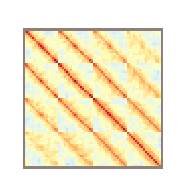
\includegraphics[width=\linewidth]{figures/stbf_struct/covs-0.eps}
      \caption{}
    \end{subfigure}\hfill%
    \begin{subfigure}{\textwidth/4}
		  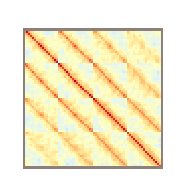
\includegraphics[width=\linewidth]{figures/stbf_struct/covs-1.eps}
      \caption{}
    \end{subfigure}\hfill%
    \begin{subfigure}{\textwidth/4}
		  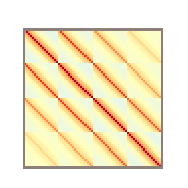
\includegraphics[width=\linewidth]{figures/stbf_struct/covs-2.eps}
      \caption{}
    \end{subfigure}\hfill%
    \begin{minipage}[b]{\textwidth/10}
      \begin{subfigure}{\textwidth}
  		  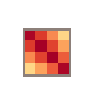
\includegraphics[width=\linewidth]{figures/stbf_struct/covs-6.eps}
        \caption{}
      \end{subfigure}\vfill%
      \begin{subfigure}{\textwidth}
  		  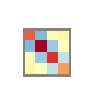
\includegraphics[width=\linewidth]{figures/stbf_struct/covs-7.eps}
        \caption{}
      \end{subfigure}\hfill%
    \end{minipage}

    \begin{subfigure}{\textwidth/4}
		  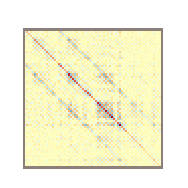
\includegraphics[width=\linewidth]{figures/stbf_struct/covs-3.eps}
      \caption{}
    \end{subfigure}\hfill%
    \begin{subfigure}{\textwidth/4}
		  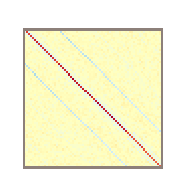
\includegraphics[width=\linewidth]{figures/stbf_struct/covs-4.eps}
      \caption{}
    \end{subfigure}\hfill%
    \begin{subfigure}{\textwidth/4}
		  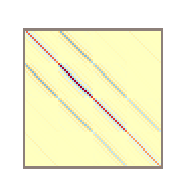
\includegraphics[width=\linewidth]{figures/stbf_struct/covs-5.eps}
      \caption{}
    \end{subfigure}\hfill%
    \begin{minipage}[b]{\textwidth/10}
      \begin{subfigure}{\textwidth}
  		  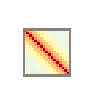
\includegraphics[width=\linewidth]{figures/stbf_struct/covs-8.eps}
        \caption{}
      \end{subfigure}\vfill%
      \begin{subfigure}{\textwidth}
  		  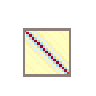
\includegraphics[width=\linewidth]{figures/stbf_struct/covs-9.eps}
        \caption{}
      \end{subfigure}\hfill%
    \end{minipage}



    \caption[Estimated covariance and inverse covariance.]{Different estimators of the covariance and inverse covariance
			of 100 epochs of data from \textit{Subject 01} for channels
			\textit{Fz}, \textit{Cz}, \textit{Pz}, and \textit{Oz} and time samples between 0.1s and 0.6s.
			Regularized estimators of the inverse covariance exhibit less extreme values and have a sparser structure.
			(\textbf{a,f}) Empirical covariance and inverse covariance matrices.
			(\textbf{b,g}) Shrunk covariance and inverse covariance matrices with $\alpha=0.14$ as
			determined by the closed-form \ac{loocv} method. (\textbf{c,h}) Kronecker-Toeplitz
			structured covariance and inverse covariance matrices.
			(\textbf{d,e}) Spatial Kronecker factor of the Kronecker-Toeplitz structured shrunk estimator and its inverse.
			(\textbf{i,j}) Temporal Kronecker factor of the Kronecker-Toeplitz structured shrunk estimator and its inverse.}
		\label{fig:kronlda-covs}
	\end{figure}

	The Kronecker approach has shown significant performance yields in different linear spatiotemporal \ac{eeg} and MEG
	applications~\cite{DeMunck2002,Huizenga2002,Beltrachini2013,GonzalezNavarro2016,GonzalezNavarro2017}.
	\textcite{Vliet2020} have applied a Kronecker-structured covariance estimator to \ac{erp} classification with linear models in a post-hoc fashion.
	Our work goes further by embedding the Kronecker structure in the
	spatiotemporal beamformer training process, using a data-adaptive shrinkage
	method, and regularizing the covariance further by imposing a Toeplitz
	structure on the temporal covariance.

	\subsubsection{Kronecker-Toeplitz structured covariance estimation}
	\label{sec:stbf-struct/methods/struct-cov}
  The question remains how to estimate $\mat{\hat{S}}$ and $\mat{\hat{T}}$.
	While the Flip-Flop and Non-iterative Flip-Flop
	algorithms~\cite{Lu2005, Werner2008, Wirfaelt2010} can estimate Kronecker or Kronecker-Toeplitz structured covariances, new results show that a fixed point iteration is more efficient~\cite{Wiesel2012a,Wiesel2012}.
	After each iteration, the spatial and temporal covariances matrices are scaled to unit
	variance to ensure the fixed point iteration converges.
	Finally, shrinkage can also be introduced in the Fixed Point Iteration to
	improve stability and achieve more robust
	regularization~\cite{Wiesel2012,Greenewald2014,Beltrachini2013, Breloy2016}.
	The spatial and temporal covariance matrices are shrunk at every fixed-point
	iteration with shrinkage factors $\beta_k$ and $\gamma_k$ before matrix
	inversion in the
	next iteration.

	Combined, this leads to the iterative estimation algorithm described by the
	following equations:
	\begin{subequations}
		\begin{equation}
      \tilde{\mat{S}}_{k+1} =
			\frac{1}{N}
      \sum^N_{n=1}\mat{X}_n^\intercal\hat{\mat{T}}_k^+\mat{X}_n
			\label{eq:stbf-struct/fpi-spatial}
		\end{equation}
		\begin{equation}
      \tilde{\mat{T}}_{k+1} =
			\frac{1}{N}
      \sum^N_{n=1}\mat{X}_n\hat{\mat{S}}_k^+\mat{X}_n^\intercal
			\label{eq:stbf-struct/fpi-temporal}
		\end{equation}
	\end{subequations}
	\begin{subequations}
		\begin{equation}
      \tilde{\mat{S}}_{k+1}^{(\beta)} =
      (1-\beta_{k+1})\tilde{\mat{S}}_{k+1}
      +\beta_{k+1}\frac{\Tr(\tilde{\mat{S}}_{k+1})}{C}\mathbb{I}
			\label{eq:stbf-struct/fpi-spatial-shrunk}
		\end{equation}
		\begin{equation}
      \tilde{\mat{T}}_{k+1}^{(\gamma)} =
      (1-\gamma_{k+1})\tilde{\mat{T}}_{k+1}
      +\gamma_{k+1}\frac{\Tr(\tilde{\mat{T}}_{k+1})}{S}\mathbb{I}
			\label{eq:stbf-struct/fpi-temporal-shrunk}
		\end{equation}
	\end{subequations}
	\begin{subequations}
		\begin{equation}
      \hat{\mat{S}}_{k+1} =
      \frac{C}{\Tr\left[\tilde{\mat{S}}_{k+1}^{(\beta)}\right]}
      \tilde{\mat{S}}_{k+1}^{(\beta)}
			\label{eq:stbf-struct/fpi-spatial-norm}
		\end{equation}
		\begin{equation}
      \hat{\mat{T}}_{k+1} =
      \frac{S}{\Tr\left[\tilde{\mat{T}}_{k+1}^{(\gamma)}\right]}
      \tilde{\mat{T}}_{k+1}^{(\gamma)}
			\label{eq:stbf-struct/fpi-temporal-norm}
		\end{equation}
	\end{subequations}
  $\hat{\mat{S}}_0$ and $\hat{\mat{T}}_0$ can be initialized to any positive definite matrix.
	We choose to use the identity matrices $\mathbb{I}^{C\times C}$ and $\mathbb{I}^{S\times S}$.
  After each iteration, all diagonals of $\hat{\mat{R}}_{k+1}$ are set to their mean
  values to ensure that $\hat{\mat{R}}_{k+1}$ and $\hat{\mat{T}}_{k+1}$ are Toeplitz structured.

	\textcite{Xie2021} show that the \ac{loocv} estimates for the
	optimal values of $\beta_{k+1}$ and $\gamma_{k+1}$ also yield a closed-form
	solution for the Kronecker fixed-point-iteration algorithm:

	\begin{subequations}
		\begin{equation}
			\beta_{k+1} =
			1-
			\frac{
        \splitfrac{
          \frac{N}{N-1}\Tr(\tilde{\mat{\hat{\S}}}_{k+1}^2)
          - \frac{2}{C}\left[\Tr(\mat{\tilde{S}}_{k+1})\right]^2
          + \frac{1}{C}\Tr(\tilde{\mat{S}}_{k+1}^2)
        }{%
				  - \frac{1}{N(N-1)}\sum_{i=1}^N
          \left[\Tr(\mat{X}_i\hat{\mat{T}}_k^+\mat{X}_i^\intercal)^2\right]
        }
			}{
        \splitfrac{
          \frac{N^2-2N}{(N-1)^2}\Tr(\tilde{\mat{S}}_{k+1}^2)
          - \frac{2}{C}\left[\Tr(\tilde{\mat{S}}_{k+1})\right]^2
          + \frac{1}{C}\Tr(\tilde{\mat{S}}_{k+1}^2)
        }{%
				  + \frac{1}{N(N-1)^2}\sum_{i=1}^N
          \left[\Tr(\mat{X}_i\hat{\mat{T}}_k^+\mat{X}_i^\intercal)^2\right]
        }
			}
			\label{eq:stbf-struct/spatial-shrinkage}
		\end{equation}
		\begin{equation}
			\gamma_{k+1} =
			1-
			\frac{
        \splitfrac{
          \frac{N}{N-1}\Tr(\tilde{\mat{T}}_{k+1}^2)
          - \frac{2}{S}\left[\Tr(\tilde{\mat{T}}_{k+1})\right]^2
          + \frac{1}{S}\Tr(\tilde{\mat{T}}_{k+1}^2)
        }{%
				  - \frac{1}{N(N-1)}\sum_{n=1}^N
          \left[\Tr(\mat{X}_n^\intercal\mat{\mat{S}}_k^+\mat{X}_n)^2\right]
        }
			}{
        \splitfrac{
          \frac{N^2-2N}{(N-1)^2}\Tr(\tilde{\mat{T}}_{k+1}^2)
          - \frac{2}{S}\left[\Tr(\tilde{\mat{T}}_{k+1})\right]^2
          + \frac{1}{S}\Tr(\tilde{\mat{T}}_{k+1}^2)
        }{
				  + \frac{1}{N(N-1)^2}\sum_{n=1}^N
          \left[\Tr(\mat{X}_n^\intercal\hat{\mat{S}}_k^+\mat{X}_n)^2\right]
        }
			}
			\label{eq:stbf-struct/temporal-shrinkage}
		\end{equation}
	\end{subequations}
	The shrinkage parameters $0<\beta_{k+1}<1$ and $0<\gamma_{k+1}<1$ should be
	re-determined after each iteration.
	The Oracle Approximation Shrinkage method can also be used to determine
	$\beta_{k+1}$ and $\gamma_{k+1}$~\cite{Chen2010,Xie2021} but performs worse for spatiotemporal \ac{eeg} data since not all assumptions are met.

	\subsection{Dataset}
	We use the dataset from~\textcite{Wittevrongel2016}, containing P3 oddball \ac{eeg}
	recordings of 21 healthy subjects since it is a high-quality dataset with a high
	number (32) of electrodes and concurrently recorded EOG responses for ocular artifact rejection.
	Nine targets were arranged on a monitor before the subject during an
	experimental session.
	The subject was asked to pay attention to a cued target for a block
	of stimulations.
	The stimulations in a block are organized in 15 separate subsequent trials.
	A trial is defined as 9 stimulations in which each target is flashed
	precisely once per trial.
	Each target was cued four times, resulting in a dataset consisting of 36 blocks
	(4860 stimulations) per subject.
	Each stimulation will correspond to a single epoch in the preprocessed dataset.
	See~\textcite{Wittevrongel2016} for a complete description of the dataset and the recording procedure.

	\subsection{Software and preprocessing}
	Data processing and classifier analysis were performed in Python using
	Scikit-Learn (version 1.0.1)~\cite{Pedregosa2011} and SciPy (version
	1.7.1)~\cite{Virtanen2020}.
	The preprocessing pipeline was implemented using the MNE-Python toolbox
	(version 0.24.0)~\cite{Gramfort2013}.
	The dataset was converted to BIDS-\ac{eeg} format~\cite{Pernet2019} and managed and
	loaded with MNE-BIDS (version 0.9)~\cite{Appelhoff2019}.
	The Riemannian classifier from \cref{sec:riemannian} was implemented using
	pyRiemann (version 0.2.7).
	Statistical tests were performed in R (version 4.1.2).

	The \ac{eeg} recorded at 2048 Hz was re-referenced off-line to the average of the mastoids.
	The reference electrodes were dropped from the analysis.
	Data were subsequently filtered between 0.5 Hz and 16 Hz using forward-backward
	filtering with a fourth-order Butterworth IIR filter.
	The \ac{eeg} signal was corrected for ocular artifacts using Independent Component
	Analysis (ICA) by rejecting components that correlated with the bipolar EOG
  channels vEOG and hEOG using iterative Z-score thresholding.
  Components with a Z-scored pearson correlation coefficient
  exceeding  3 times the standard deviation of the Z-scored
  correlation coefficients of other components, were iteratively
  rejected until none that exceed the threshold remained.
  Finally, epochs were cut from 0.1s to 0.6s after stimulus onset.
	No baseline correction was performed since this affects the temporal covariance
	of the data, violating the Toeplitz structure assumption~\cite{Bijma2003}.

	\subsection{Classification}
	\subsubsection{Cross-validation scheme per subject}
	We use a variation of grouped fold cross-validation per subject to evaluate the classifiers.
	We apply 4-fold cross-validation by splitting the blocks of each subject into
	four continuous folds.
	Unlike regular cross-validation, we only use a single fold to train the
	classifiers while using the other three folds for validation.
	This scheme results in a training set of 9 blocks of 135 epochs each.
	We chose this approach since we are primarily interested in the performance of the classifiers in the case of low data availability.
	The classification task is to determine the cued target for each block.
	The fraction of correctly predicted cues provides the accuracy of a classifier.
	Data from all trials are used in the training fold, while classifier validation
	is performed multiple times per fold, each time using an increasing amount of
	trials (i.e., using the first trial, using the first two trials, etc. until all 15 trials
	are used).
	For each of the 9 stimulated targets, the averages over the corresponding epochs across
	the utilized trials are used to predict the cued target in that block.
	The target with the maximal classifier score was then chosen as the predicted
	cued target.
	Before training the classifiers, a Z-score normalization transformation was
	developed on the training data to scale all \ac{eeg} channels to unit variance.
	This transformation was then applied to the validation data.

  \subsubsection{\Acl{stbf} classifier}
	Before calculating the \ac{stbf}, the signal was downsampled to
	32 Hz or twice the low-pass frequency 16 Hz, resulting in 17 time samples
	between 0.1 and 0.6s. According to the Nyquist Theorem, more samples would not
	contain more information hence the minimum temporal resolution is chosen to reduce
	the dimensionality of the covariance and improve its condition number.
	The activation pattern is the difference between the averages of epochs in response to cued targets and the averages of those in response to non-cued targets.
	We constructed three variations of the spatiotemporal beamformer the \ac{stbf-emp} as in
	\cref{sec:stbf-struct/methods/emp-cov}, the \ac{stbf-shrunk} as in
	\cref{sec:stbf-struct/methods/shrunk-cov}, and the \ac{stbf-struct} with \ac{loocv} shrinkage for
	the Kronecker factors as in \cref{sec:stbf-struct/methods/struct-cov}.

	\subsubsection{Riemannian geometry classifier}
	\label{sec:riemannian}
	We opted for a Riemannian
	geometry-based classifier to compare our results.
	The Riemannian model (XDAWN+RG) uses the XDAWN spatial filter combined
	with Riemannian geometry in tangent space as implemented by Barachant et
	al.~\cite{Barachant2014a}.
	This classifier uses four XDAWN spatial filters and each epoch's empirical spatial covariance matrix.
	The target with the maximum score is the prediction of the cued target.
	XDAWN+RG was trained and validated without downsampling using epochs
	at the original sample rate of 2048 Hz.
  Preliminary experimentation revealed that best performance in low and high
  data availability setting was achieved when no shrinkage was applied to the estimation of XDAWN filters or the subsequent
  covariance matrices for this specific dataset.
  Hence, no shrinkage regularization will be applied to XDAWN+RG in
  further experiments.

	\section{Results}
	\subsection{Minimum required fixed-point iterations}
	The fixed point iteration algorithm described
	in
  \crefrange{eq:stbf-struct/fpi-spatial}{eq:stbf-struct/fpi-temporal-norm}
  estimates the Kronecker-Toeplitz structured covariance for the
	\ac{stbf-struct} classifier.
	Fixed-point iteration is an iterative procedure starting from (in our case)
	non-informed initial guesses for the spatial and temporal covariance matrices.
	As a stopping criterion, one could impose a threshold on the difference in
	outcome of successive steps, e.g., based on the covariance norm or the
	classifier accuracy.
	However, few iterations or even just one~\cite{Castaneda2014} suffice to achieve satisfactory performance in practice.

	\cref{fig:iterations} confirms these results for the \ac{stbf-struct} classifier.
	Using more than one fixed-point iteration does not significantly improve the
	accuracy across the amounts of training data and the number of trials
  used for evaluation.
	Hence, only one iteration is used for the \ac{stbf-struct} classifier, leading to a drastic speed-up of
  the  training process.

  \begin{figure}[t]
    \begin{subfigure}{\linewidth}
      \hspace{-0.4623567780166823in}
%% Creator: Matplotlib, PGF backend
%%
%% To include the figure in your LaTeX document, write
%%   \input{<filename>.pgf}
%%
%% Make sure the required packages are loaded in your preamble
%%   \usepackage{pgf}
%%
%% Also ensure that all the required font packages are loaded; for instance,
%% the lmodern package is sometimes necessary when using math font.
%%   \usepackage{lmodern}
%%
%% Figures using additional raster images can only be included by \input if
%% they are in the same directory as the main LaTeX file. For loading figures
%% from other directories you can use the `import` package
%%   \usepackage{import}
%%
%% and then include the figures with
%%   \import{<path to file>}{<filename>.pgf}
%%
%% Matplotlib used the following preamble
%%
\begingroup%
\makeatletter%
\begin{pgfpicture}%
\pgfpathrectangle{\pgfpointorigin}{\pgfqpoint{4.788446in}{1.097570in}}%
\pgfusepath{use as bounding box, clip}%
\begin{pgfscope}%
\pgfsetbuttcap%
\pgfsetmiterjoin%
\definecolor{currentfill}{rgb}{1.000000,1.000000,1.000000}%
\pgfsetfillcolor{currentfill}%
\pgfsetlinewidth{0.000000pt}%
\definecolor{currentstroke}{rgb}{1.000000,1.000000,1.000000}%
\pgfsetstrokecolor{currentstroke}%
\pgfsetdash{}{0pt}%
\pgfpathmoveto{\pgfqpoint{0.000000in}{0.000000in}}%
\pgfpathlineto{\pgfqpoint{4.788446in}{0.000000in}}%
\pgfpathlineto{\pgfqpoint{4.788446in}{1.097570in}}%
\pgfpathlineto{\pgfqpoint{0.000000in}{1.097570in}}%
\pgfpathlineto{\pgfqpoint{0.000000in}{0.000000in}}%
\pgfpathclose%
\pgfusepath{fill}%
\end{pgfscope}%
\begin{pgfscope}%
\pgfsetbuttcap%
\pgfsetmiterjoin%
\definecolor{currentfill}{rgb}{1.000000,1.000000,1.000000}%
\pgfsetfillcolor{currentfill}%
\pgfsetlinewidth{0.000000pt}%
\definecolor{currentstroke}{rgb}{0.000000,0.000000,0.000000}%
\pgfsetstrokecolor{currentstroke}%
\pgfsetstrokeopacity{0.000000}%
\pgfsetdash{}{0pt}%
\pgfpathmoveto{\pgfqpoint{0.421874in}{0.067708in}}%
\pgfpathlineto{\pgfqpoint{1.821838in}{0.067708in}}%
\pgfpathlineto{\pgfqpoint{1.821838in}{0.927431in}}%
\pgfpathlineto{\pgfqpoint{0.421874in}{0.927431in}}%
\pgfpathlineto{\pgfqpoint{0.421874in}{0.067708in}}%
\pgfpathclose%
\pgfusepath{fill}%
\end{pgfscope}%
\begin{pgfscope}%
\pgfpathrectangle{\pgfqpoint{0.421874in}{0.067708in}}{\pgfqpoint{1.399964in}{0.859723in}}%
\pgfusepath{clip}%
\pgfsetbuttcap%
\pgfsetroundjoin%
\definecolor{currentfill}{rgb}{0.949020,0.564706,0.094118}%
\pgfsetfillcolor{currentfill}%
\pgfsetfillopacity{0.200000}%
\pgfsetlinewidth{1.003750pt}%
\definecolor{currentstroke}{rgb}{0.949020,0.564706,0.094118}%
\pgfsetstrokecolor{currentstroke}%
\pgfsetstrokeopacity{0.200000}%
\pgfsetdash{}{0pt}%
\pgfsys@defobject{currentmarker}{\pgfqpoint{0.485508in}{0.247765in}}{\pgfqpoint{1.758203in}{0.398254in}}{%
\pgfpathmoveto{\pgfqpoint{0.485508in}{0.288704in}}%
\pgfpathlineto{\pgfqpoint{0.485508in}{0.247765in}}%
\pgfpathlineto{\pgfqpoint{0.612778in}{0.336457in}}%
\pgfpathlineto{\pgfqpoint{0.740047in}{0.342911in}}%
\pgfpathlineto{\pgfqpoint{0.867317in}{0.337594in}}%
\pgfpathlineto{\pgfqpoint{0.994586in}{0.339120in}}%
\pgfpathlineto{\pgfqpoint{1.121856in}{0.338722in}}%
\pgfpathlineto{\pgfqpoint{1.249125in}{0.335301in}}%
\pgfpathlineto{\pgfqpoint{1.376395in}{0.335320in}}%
\pgfpathlineto{\pgfqpoint{1.503664in}{0.333434in}}%
\pgfpathlineto{\pgfqpoint{1.630934in}{0.334562in}}%
\pgfpathlineto{\pgfqpoint{1.758203in}{0.335708in}}%
\pgfpathlineto{\pgfqpoint{1.758203in}{0.393715in}}%
\pgfpathlineto{\pgfqpoint{1.758203in}{0.393715in}}%
\pgfpathlineto{\pgfqpoint{1.630934in}{0.390673in}}%
\pgfpathlineto{\pgfqpoint{1.503664in}{0.392957in}}%
\pgfpathlineto{\pgfqpoint{1.376395in}{0.394464in}}%
\pgfpathlineto{\pgfqpoint{1.249125in}{0.391810in}}%
\pgfpathlineto{\pgfqpoint{1.121856in}{0.394094in}}%
\pgfpathlineto{\pgfqpoint{0.994586in}{0.393326in}}%
\pgfpathlineto{\pgfqpoint{0.867317in}{0.394473in}}%
\pgfpathlineto{\pgfqpoint{0.740047in}{0.398254in}}%
\pgfpathlineto{\pgfqpoint{0.612778in}{0.395231in}}%
\pgfpathlineto{\pgfqpoint{0.485508in}{0.288704in}}%
\pgfpathlineto{\pgfqpoint{0.485508in}{0.288704in}}%
\pgfpathclose%
\pgfusepath{stroke,fill}%
}%
\begin{pgfscope}%
\pgfsys@transformshift{0.000000in}{0.000000in}%
\pgfsys@useobject{currentmarker}{}%
\end{pgfscope}%
\end{pgfscope}%
\begin{pgfscope}%
\pgfsetbuttcap%
\pgfsetroundjoin%
\definecolor{currentfill}{rgb}{0.552941,0.501961,0.478431}%
\pgfsetfillcolor{currentfill}%
\pgfsetlinewidth{0.803000pt}%
\definecolor{currentstroke}{rgb}{0.552941,0.501961,0.478431}%
\pgfsetstrokecolor{currentstroke}%
\pgfsetdash{}{0pt}%
\pgfsys@defobject{currentmarker}{\pgfqpoint{0.000000in}{0.000000in}}{\pgfqpoint{0.000000in}{0.041667in}}{%
\pgfpathmoveto{\pgfqpoint{0.000000in}{0.000000in}}%
\pgfpathlineto{\pgfqpoint{0.000000in}{0.041667in}}%
\pgfusepath{stroke,fill}%
}%
\begin{pgfscope}%
\pgfsys@transformshift{0.485508in}{0.067708in}%
\pgfsys@useobject{currentmarker}{}%
\end{pgfscope}%
\end{pgfscope}%
\begin{pgfscope}%
\pgfsetbuttcap%
\pgfsetroundjoin%
\definecolor{currentfill}{rgb}{0.552941,0.501961,0.478431}%
\pgfsetfillcolor{currentfill}%
\pgfsetlinewidth{0.803000pt}%
\definecolor{currentstroke}{rgb}{0.552941,0.501961,0.478431}%
\pgfsetstrokecolor{currentstroke}%
\pgfsetdash{}{0pt}%
\pgfsys@defobject{currentmarker}{\pgfqpoint{0.000000in}{0.000000in}}{\pgfqpoint{0.000000in}{0.041667in}}{%
\pgfpathmoveto{\pgfqpoint{0.000000in}{0.000000in}}%
\pgfpathlineto{\pgfqpoint{0.000000in}{0.041667in}}%
\pgfusepath{stroke,fill}%
}%
\begin{pgfscope}%
\pgfsys@transformshift{0.740047in}{0.067708in}%
\pgfsys@useobject{currentmarker}{}%
\end{pgfscope}%
\end{pgfscope}%
\begin{pgfscope}%
\pgfsetbuttcap%
\pgfsetroundjoin%
\definecolor{currentfill}{rgb}{0.552941,0.501961,0.478431}%
\pgfsetfillcolor{currentfill}%
\pgfsetlinewidth{0.803000pt}%
\definecolor{currentstroke}{rgb}{0.552941,0.501961,0.478431}%
\pgfsetstrokecolor{currentstroke}%
\pgfsetdash{}{0pt}%
\pgfsys@defobject{currentmarker}{\pgfqpoint{0.000000in}{0.000000in}}{\pgfqpoint{0.000000in}{0.041667in}}{%
\pgfpathmoveto{\pgfqpoint{0.000000in}{0.000000in}}%
\pgfpathlineto{\pgfqpoint{0.000000in}{0.041667in}}%
\pgfusepath{stroke,fill}%
}%
\begin{pgfscope}%
\pgfsys@transformshift{0.994586in}{0.067708in}%
\pgfsys@useobject{currentmarker}{}%
\end{pgfscope}%
\end{pgfscope}%
\begin{pgfscope}%
\pgfsetbuttcap%
\pgfsetroundjoin%
\definecolor{currentfill}{rgb}{0.552941,0.501961,0.478431}%
\pgfsetfillcolor{currentfill}%
\pgfsetlinewidth{0.803000pt}%
\definecolor{currentstroke}{rgb}{0.552941,0.501961,0.478431}%
\pgfsetstrokecolor{currentstroke}%
\pgfsetdash{}{0pt}%
\pgfsys@defobject{currentmarker}{\pgfqpoint{0.000000in}{0.000000in}}{\pgfqpoint{0.000000in}{0.041667in}}{%
\pgfpathmoveto{\pgfqpoint{0.000000in}{0.000000in}}%
\pgfpathlineto{\pgfqpoint{0.000000in}{0.041667in}}%
\pgfusepath{stroke,fill}%
}%
\begin{pgfscope}%
\pgfsys@transformshift{1.249125in}{0.067708in}%
\pgfsys@useobject{currentmarker}{}%
\end{pgfscope}%
\end{pgfscope}%
\begin{pgfscope}%
\pgfsetbuttcap%
\pgfsetroundjoin%
\definecolor{currentfill}{rgb}{0.552941,0.501961,0.478431}%
\pgfsetfillcolor{currentfill}%
\pgfsetlinewidth{0.803000pt}%
\definecolor{currentstroke}{rgb}{0.552941,0.501961,0.478431}%
\pgfsetstrokecolor{currentstroke}%
\pgfsetdash{}{0pt}%
\pgfsys@defobject{currentmarker}{\pgfqpoint{0.000000in}{0.000000in}}{\pgfqpoint{0.000000in}{0.041667in}}{%
\pgfpathmoveto{\pgfqpoint{0.000000in}{0.000000in}}%
\pgfpathlineto{\pgfqpoint{0.000000in}{0.041667in}}%
\pgfusepath{stroke,fill}%
}%
\begin{pgfscope}%
\pgfsys@transformshift{1.503664in}{0.067708in}%
\pgfsys@useobject{currentmarker}{}%
\end{pgfscope}%
\end{pgfscope}%
\begin{pgfscope}%
\pgfsetbuttcap%
\pgfsetroundjoin%
\definecolor{currentfill}{rgb}{0.552941,0.501961,0.478431}%
\pgfsetfillcolor{currentfill}%
\pgfsetlinewidth{0.803000pt}%
\definecolor{currentstroke}{rgb}{0.552941,0.501961,0.478431}%
\pgfsetstrokecolor{currentstroke}%
\pgfsetdash{}{0pt}%
\pgfsys@defobject{currentmarker}{\pgfqpoint{0.000000in}{0.000000in}}{\pgfqpoint{0.000000in}{0.041667in}}{%
\pgfpathmoveto{\pgfqpoint{0.000000in}{0.000000in}}%
\pgfpathlineto{\pgfqpoint{0.000000in}{0.041667in}}%
\pgfusepath{stroke,fill}%
}%
\begin{pgfscope}%
\pgfsys@transformshift{1.758203in}{0.067708in}%
\pgfsys@useobject{currentmarker}{}%
\end{pgfscope}%
\end{pgfscope}%
\begin{pgfscope}%
\pgfsetbuttcap%
\pgfsetroundjoin%
\definecolor{currentfill}{rgb}{0.552941,0.501961,0.478431}%
\pgfsetfillcolor{currentfill}%
\pgfsetlinewidth{0.803000pt}%
\definecolor{currentstroke}{rgb}{0.552941,0.501961,0.478431}%
\pgfsetstrokecolor{currentstroke}%
\pgfsetdash{}{0pt}%
\pgfsys@defobject{currentmarker}{\pgfqpoint{0.000000in}{0.000000in}}{\pgfqpoint{0.041667in}{0.000000in}}{%
\pgfpathmoveto{\pgfqpoint{0.000000in}{0.000000in}}%
\pgfpathlineto{\pgfqpoint{0.041667in}{0.000000in}}%
\pgfusepath{stroke,fill}%
}%
\begin{pgfscope}%
\pgfsys@transformshift{0.421874in}{0.067708in}%
\pgfsys@useobject{currentmarker}{}%
\end{pgfscope}%
\end{pgfscope}%
\begin{pgfscope}%
\definecolor{textcolor}{rgb}{0.552941,0.501961,0.478431}%
\pgfsetstrokecolor{textcolor}%
\pgfsetfillcolor{textcolor}%
\pgftext[x=0.309027in, y=0.024306in, left, base]{\color{textcolor}\sffamily\fontsize{9.000000}{10.800000}\selectfont 0}%
\end{pgfscope}%
\begin{pgfscope}%
\pgfsetbuttcap%
\pgfsetroundjoin%
\definecolor{currentfill}{rgb}{0.552941,0.501961,0.478431}%
\pgfsetfillcolor{currentfill}%
\pgfsetlinewidth{0.803000pt}%
\definecolor{currentstroke}{rgb}{0.552941,0.501961,0.478431}%
\pgfsetstrokecolor{currentstroke}%
\pgfsetdash{}{0pt}%
\pgfsys@defobject{currentmarker}{\pgfqpoint{0.000000in}{0.000000in}}{\pgfqpoint{0.041667in}{0.000000in}}{%
\pgfpathmoveto{\pgfqpoint{0.000000in}{0.000000in}}%
\pgfpathlineto{\pgfqpoint{0.041667in}{0.000000in}}%
\pgfusepath{stroke,fill}%
}%
\begin{pgfscope}%
\pgfsys@transformshift{0.421874in}{0.497570in}%
\pgfsys@useobject{currentmarker}{}%
\end{pgfscope}%
\end{pgfscope}%
\begin{pgfscope}%
\definecolor{textcolor}{rgb}{0.552941,0.501961,0.478431}%
\pgfsetstrokecolor{textcolor}%
\pgfsetfillcolor{textcolor}%
\pgftext[x=0.244791in, y=0.454167in, left, base]{\color{textcolor}\sffamily\fontsize{9.000000}{10.800000}\selectfont 50}%
\end{pgfscope}%
\begin{pgfscope}%
\pgfsetbuttcap%
\pgfsetroundjoin%
\definecolor{currentfill}{rgb}{0.552941,0.501961,0.478431}%
\pgfsetfillcolor{currentfill}%
\pgfsetlinewidth{0.803000pt}%
\definecolor{currentstroke}{rgb}{0.552941,0.501961,0.478431}%
\pgfsetstrokecolor{currentstroke}%
\pgfsetdash{}{0pt}%
\pgfsys@defobject{currentmarker}{\pgfqpoint{0.000000in}{0.000000in}}{\pgfqpoint{0.041667in}{0.000000in}}{%
\pgfpathmoveto{\pgfqpoint{0.000000in}{0.000000in}}%
\pgfpathlineto{\pgfqpoint{0.041667in}{0.000000in}}%
\pgfusepath{stroke,fill}%
}%
\begin{pgfscope}%
\pgfsys@transformshift{0.421874in}{0.927431in}%
\pgfsys@useobject{currentmarker}{}%
\end{pgfscope}%
\end{pgfscope}%
\begin{pgfscope}%
\definecolor{textcolor}{rgb}{0.552941,0.501961,0.478431}%
\pgfsetstrokecolor{textcolor}%
\pgfsetfillcolor{textcolor}%
\pgftext[x=0.180556in, y=0.884028in, left, base]{\color{textcolor}\sffamily\fontsize{9.000000}{10.800000}\selectfont 100}%
\end{pgfscope}%
\begin{pgfscope}%
\definecolor{textcolor}{rgb}{0.552941,0.501961,0.478431}%
\pgfsetstrokecolor{textcolor}%
\pgfsetfillcolor{textcolor}%
\pgftext[x=0.125000in,y=0.497570in,,bottom,rotate=90.000000]{\color{textcolor}\sffamily\fontsize{9.000000}{10.800000}\selectfont Accuracy (\%)}%
\end{pgfscope}%
\begin{pgfscope}%
\pgfpathrectangle{\pgfqpoint{0.421874in}{0.067708in}}{\pgfqpoint{1.399964in}{0.859723in}}%
\pgfusepath{clip}%
\pgfsetrectcap%
\pgfsetroundjoin%
\pgfsetlinewidth{1.505625pt}%
\definecolor{currentstroke}{rgb}{0.949020,0.564706,0.094118}%
\pgfsetstrokecolor{currentstroke}%
\pgfsetdash{}{0pt}%
\pgfpathmoveto{\pgfqpoint{0.485508in}{0.267476in}}%
\pgfpathlineto{\pgfqpoint{0.612778in}{0.366034in}}%
\pgfpathlineto{\pgfqpoint{0.740047in}{0.370582in}}%
\pgfpathlineto{\pgfqpoint{0.867317in}{0.366413in}}%
\pgfpathlineto{\pgfqpoint{0.994586in}{0.366792in}}%
\pgfpathlineto{\pgfqpoint{1.121856in}{0.365276in}}%
\pgfpathlineto{\pgfqpoint{1.249125in}{0.363759in}}%
\pgfpathlineto{\pgfqpoint{1.376395in}{0.363001in}}%
\pgfpathlineto{\pgfqpoint{1.503664in}{0.363001in}}%
\pgfpathlineto{\pgfqpoint{1.630934in}{0.363001in}}%
\pgfpathlineto{\pgfqpoint{1.758203in}{0.363380in}}%
\pgfusepath{stroke}%
\end{pgfscope}%
\begin{pgfscope}%
\pgfpathrectangle{\pgfqpoint{0.421874in}{0.067708in}}{\pgfqpoint{1.399964in}{0.859723in}}%
\pgfusepath{clip}%
\pgfsetbuttcap%
\pgfsetmiterjoin%
\definecolor{currentfill}{rgb}{0.949020,0.564706,0.094118}%
\pgfsetfillcolor{currentfill}%
\pgfsetlinewidth{0.000000pt}%
\definecolor{currentstroke}{rgb}{1.000000,1.000000,1.000000}%
\pgfsetstrokecolor{currentstroke}%
\pgfsetdash{}{0pt}%
\pgfsys@defobject{currentmarker}{\pgfqpoint{-0.020833in}{-0.020833in}}{\pgfqpoint{0.020833in}{0.020833in}}{%
\pgfpathmoveto{\pgfqpoint{-0.020833in}{-0.020833in}}%
\pgfpathlineto{\pgfqpoint{0.020833in}{-0.020833in}}%
\pgfpathlineto{\pgfqpoint{0.020833in}{0.020833in}}%
\pgfpathlineto{\pgfqpoint{-0.020833in}{0.020833in}}%
\pgfpathlineto{\pgfqpoint{-0.020833in}{-0.020833in}}%
\pgfpathclose%
\pgfusepath{fill}%
}%
\begin{pgfscope}%
\pgfsys@transformshift{0.485508in}{0.267476in}%
\pgfsys@useobject{currentmarker}{}%
\end{pgfscope}%
\begin{pgfscope}%
\pgfsys@transformshift{0.612778in}{0.366034in}%
\pgfsys@useobject{currentmarker}{}%
\end{pgfscope}%
\begin{pgfscope}%
\pgfsys@transformshift{0.740047in}{0.370582in}%
\pgfsys@useobject{currentmarker}{}%
\end{pgfscope}%
\begin{pgfscope}%
\pgfsys@transformshift{0.867317in}{0.366413in}%
\pgfsys@useobject{currentmarker}{}%
\end{pgfscope}%
\begin{pgfscope}%
\pgfsys@transformshift{0.994586in}{0.366792in}%
\pgfsys@useobject{currentmarker}{}%
\end{pgfscope}%
\begin{pgfscope}%
\pgfsys@transformshift{1.121856in}{0.365276in}%
\pgfsys@useobject{currentmarker}{}%
\end{pgfscope}%
\begin{pgfscope}%
\pgfsys@transformshift{1.249125in}{0.363759in}%
\pgfsys@useobject{currentmarker}{}%
\end{pgfscope}%
\begin{pgfscope}%
\pgfsys@transformshift{1.376395in}{0.363001in}%
\pgfsys@useobject{currentmarker}{}%
\end{pgfscope}%
\begin{pgfscope}%
\pgfsys@transformshift{1.503664in}{0.363001in}%
\pgfsys@useobject{currentmarker}{}%
\end{pgfscope}%
\begin{pgfscope}%
\pgfsys@transformshift{1.630934in}{0.363001in}%
\pgfsys@useobject{currentmarker}{}%
\end{pgfscope}%
\begin{pgfscope}%
\pgfsys@transformshift{1.758203in}{0.363380in}%
\pgfsys@useobject{currentmarker}{}%
\end{pgfscope}%
\end{pgfscope}%
\begin{pgfscope}%
\pgfpathrectangle{\pgfqpoint{0.421874in}{0.067708in}}{\pgfqpoint{1.399964in}{0.859723in}}%
\pgfusepath{clip}%
\pgfsetbuttcap%
\pgfsetroundjoin%
\pgfsetlinewidth{1.003750pt}%
\definecolor{currentstroke}{rgb}{0.878431,0.878431,0.878431}%
\pgfsetstrokecolor{currentstroke}%
\pgfsetdash{{3.700000pt}{1.600000pt}}{0.000000pt}%
\pgfpathmoveto{\pgfqpoint{0.421874in}{0.163233in}}%
\pgfpathlineto{\pgfqpoint{1.821838in}{0.163233in}}%
\pgfusepath{stroke}%
\end{pgfscope}%
\begin{pgfscope}%
\pgfsetrectcap%
\pgfsetmiterjoin%
\pgfsetlinewidth{0.803000pt}%
\definecolor{currentstroke}{rgb}{0.552941,0.501961,0.478431}%
\pgfsetstrokecolor{currentstroke}%
\pgfsetdash{}{0pt}%
\pgfpathmoveto{\pgfqpoint{0.421874in}{0.067708in}}%
\pgfpathlineto{\pgfqpoint{0.421874in}{0.927431in}}%
\pgfusepath{stroke}%
\end{pgfscope}%
\begin{pgfscope}%
\pgfsetrectcap%
\pgfsetmiterjoin%
\pgfsetlinewidth{0.803000pt}%
\definecolor{currentstroke}{rgb}{0.552941,0.501961,0.478431}%
\pgfsetstrokecolor{currentstroke}%
\pgfsetdash{}{0pt}%
\pgfpathmoveto{\pgfqpoint{1.821838in}{0.067708in}}%
\pgfpathlineto{\pgfqpoint{1.821838in}{0.927431in}}%
\pgfusepath{stroke}%
\end{pgfscope}%
\begin{pgfscope}%
\pgfsetrectcap%
\pgfsetmiterjoin%
\pgfsetlinewidth{0.803000pt}%
\definecolor{currentstroke}{rgb}{0.552941,0.501961,0.478431}%
\pgfsetstrokecolor{currentstroke}%
\pgfsetdash{}{0pt}%
\pgfpathmoveto{\pgfqpoint{0.421874in}{0.067708in}}%
\pgfpathlineto{\pgfqpoint{1.821838in}{0.067708in}}%
\pgfusepath{stroke}%
\end{pgfscope}%
\begin{pgfscope}%
\pgfsetrectcap%
\pgfsetmiterjoin%
\pgfsetlinewidth{0.803000pt}%
\definecolor{currentstroke}{rgb}{0.552941,0.501961,0.478431}%
\pgfsetstrokecolor{currentstroke}%
\pgfsetdash{}{0pt}%
\pgfpathmoveto{\pgfqpoint{0.421874in}{0.927431in}}%
\pgfpathlineto{\pgfqpoint{1.821838in}{0.927431in}}%
\pgfusepath{stroke}%
\end{pgfscope}%
\begin{pgfscope}%
\definecolor{textcolor}{rgb}{0.552941,0.501961,0.478431}%
\pgfsetstrokecolor{textcolor}%
\pgfsetfillcolor{textcolor}%
\pgftext[x=0.421874in,y=1.010765in,left,base]{\color{textcolor}\sffamily\fontsize{9.000000}{10.800000}\selectfont 1 trial}%
\end{pgfscope}%
\begin{pgfscope}%
\pgfsetbuttcap%
\pgfsetmiterjoin%
\definecolor{currentfill}{rgb}{1.000000,1.000000,1.000000}%
\pgfsetfillcolor{currentfill}%
\pgfsetlinewidth{0.000000pt}%
\definecolor{currentstroke}{rgb}{0.000000,0.000000,0.000000}%
\pgfsetstrokecolor{currentstroke}%
\pgfsetstrokeopacity{0.000000}%
\pgfsetdash{}{0pt}%
\pgfpathmoveto{\pgfqpoint{1.905178in}{0.067708in}}%
\pgfpathlineto{\pgfqpoint{3.305142in}{0.067708in}}%
\pgfpathlineto{\pgfqpoint{3.305142in}{0.927431in}}%
\pgfpathlineto{\pgfqpoint{1.905178in}{0.927431in}}%
\pgfpathlineto{\pgfqpoint{1.905178in}{0.067708in}}%
\pgfpathclose%
\pgfusepath{fill}%
\end{pgfscope}%
\begin{pgfscope}%
\pgfpathrectangle{\pgfqpoint{1.905178in}{0.067708in}}{\pgfqpoint{1.399964in}{0.859723in}}%
\pgfusepath{clip}%
\pgfsetbuttcap%
\pgfsetroundjoin%
\definecolor{currentfill}{rgb}{0.949020,0.564706,0.094118}%
\pgfsetfillcolor{currentfill}%
\pgfsetfillopacity{0.200000}%
\pgfsetlinewidth{1.003750pt}%
\definecolor{currentstroke}{rgb}{0.949020,0.564706,0.094118}%
\pgfsetstrokecolor{currentstroke}%
\pgfsetstrokeopacity{0.200000}%
\pgfsetdash{}{0pt}%
\pgfsys@defobject{currentmarker}{\pgfqpoint{1.968813in}{0.328885in}}{\pgfqpoint{3.241507in}{0.519177in}}{%
\pgfpathmoveto{\pgfqpoint{1.968813in}{0.390294in}}%
\pgfpathlineto{\pgfqpoint{1.968813in}{0.328885in}}%
\pgfpathlineto{\pgfqpoint{2.096082in}{0.451314in}}%
\pgfpathlineto{\pgfqpoint{2.223352in}{0.449798in}}%
\pgfpathlineto{\pgfqpoint{2.350621in}{0.448670in}}%
\pgfpathlineto{\pgfqpoint{2.477890in}{0.442605in}}%
\pgfpathlineto{\pgfqpoint{2.605160in}{0.438028in}}%
\pgfpathlineto{\pgfqpoint{2.732429in}{0.441089in}}%
\pgfpathlineto{\pgfqpoint{2.859699in}{0.441468in}}%
\pgfpathlineto{\pgfqpoint{2.986968in}{0.440331in}}%
\pgfpathlineto{\pgfqpoint{3.114238in}{0.440691in}}%
\pgfpathlineto{\pgfqpoint{3.241507in}{0.436919in}}%
\pgfpathlineto{\pgfqpoint{3.241507in}{0.513500in}}%
\pgfpathlineto{\pgfqpoint{3.241507in}{0.513500in}}%
\pgfpathlineto{\pgfqpoint{3.114238in}{0.509709in}}%
\pgfpathlineto{\pgfqpoint{2.986968in}{0.509700in}}%
\pgfpathlineto{\pgfqpoint{2.859699in}{0.510098in}}%
\pgfpathlineto{\pgfqpoint{2.732429in}{0.512353in}}%
\pgfpathlineto{\pgfqpoint{2.605160in}{0.511595in}}%
\pgfpathlineto{\pgfqpoint{2.477890in}{0.512742in}}%
\pgfpathlineto{\pgfqpoint{2.350621in}{0.514249in}}%
\pgfpathlineto{\pgfqpoint{2.223352in}{0.519177in}}%
\pgfpathlineto{\pgfqpoint{2.096082in}{0.516523in}}%
\pgfpathlineto{\pgfqpoint{1.968813in}{0.390294in}}%
\pgfpathlineto{\pgfqpoint{1.968813in}{0.390294in}}%
\pgfpathclose%
\pgfusepath{stroke,fill}%
}%
\begin{pgfscope}%
\pgfsys@transformshift{0.000000in}{0.000000in}%
\pgfsys@useobject{currentmarker}{}%
\end{pgfscope}%
\end{pgfscope}%
\begin{pgfscope}%
\pgfsetbuttcap%
\pgfsetroundjoin%
\definecolor{currentfill}{rgb}{0.552941,0.501961,0.478431}%
\pgfsetfillcolor{currentfill}%
\pgfsetlinewidth{0.803000pt}%
\definecolor{currentstroke}{rgb}{0.552941,0.501961,0.478431}%
\pgfsetstrokecolor{currentstroke}%
\pgfsetdash{}{0pt}%
\pgfsys@defobject{currentmarker}{\pgfqpoint{0.000000in}{0.000000in}}{\pgfqpoint{0.000000in}{0.041667in}}{%
\pgfpathmoveto{\pgfqpoint{0.000000in}{0.000000in}}%
\pgfpathlineto{\pgfqpoint{0.000000in}{0.041667in}}%
\pgfusepath{stroke,fill}%
}%
\begin{pgfscope}%
\pgfsys@transformshift{1.968813in}{0.067708in}%
\pgfsys@useobject{currentmarker}{}%
\end{pgfscope}%
\end{pgfscope}%
\begin{pgfscope}%
\pgfsetbuttcap%
\pgfsetroundjoin%
\definecolor{currentfill}{rgb}{0.552941,0.501961,0.478431}%
\pgfsetfillcolor{currentfill}%
\pgfsetlinewidth{0.803000pt}%
\definecolor{currentstroke}{rgb}{0.552941,0.501961,0.478431}%
\pgfsetstrokecolor{currentstroke}%
\pgfsetdash{}{0pt}%
\pgfsys@defobject{currentmarker}{\pgfqpoint{0.000000in}{0.000000in}}{\pgfqpoint{0.000000in}{0.041667in}}{%
\pgfpathmoveto{\pgfqpoint{0.000000in}{0.000000in}}%
\pgfpathlineto{\pgfqpoint{0.000000in}{0.041667in}}%
\pgfusepath{stroke,fill}%
}%
\begin{pgfscope}%
\pgfsys@transformshift{2.223352in}{0.067708in}%
\pgfsys@useobject{currentmarker}{}%
\end{pgfscope}%
\end{pgfscope}%
\begin{pgfscope}%
\pgfsetbuttcap%
\pgfsetroundjoin%
\definecolor{currentfill}{rgb}{0.552941,0.501961,0.478431}%
\pgfsetfillcolor{currentfill}%
\pgfsetlinewidth{0.803000pt}%
\definecolor{currentstroke}{rgb}{0.552941,0.501961,0.478431}%
\pgfsetstrokecolor{currentstroke}%
\pgfsetdash{}{0pt}%
\pgfsys@defobject{currentmarker}{\pgfqpoint{0.000000in}{0.000000in}}{\pgfqpoint{0.000000in}{0.041667in}}{%
\pgfpathmoveto{\pgfqpoint{0.000000in}{0.000000in}}%
\pgfpathlineto{\pgfqpoint{0.000000in}{0.041667in}}%
\pgfusepath{stroke,fill}%
}%
\begin{pgfscope}%
\pgfsys@transformshift{2.477890in}{0.067708in}%
\pgfsys@useobject{currentmarker}{}%
\end{pgfscope}%
\end{pgfscope}%
\begin{pgfscope}%
\pgfsetbuttcap%
\pgfsetroundjoin%
\definecolor{currentfill}{rgb}{0.552941,0.501961,0.478431}%
\pgfsetfillcolor{currentfill}%
\pgfsetlinewidth{0.803000pt}%
\definecolor{currentstroke}{rgb}{0.552941,0.501961,0.478431}%
\pgfsetstrokecolor{currentstroke}%
\pgfsetdash{}{0pt}%
\pgfsys@defobject{currentmarker}{\pgfqpoint{0.000000in}{0.000000in}}{\pgfqpoint{0.000000in}{0.041667in}}{%
\pgfpathmoveto{\pgfqpoint{0.000000in}{0.000000in}}%
\pgfpathlineto{\pgfqpoint{0.000000in}{0.041667in}}%
\pgfusepath{stroke,fill}%
}%
\begin{pgfscope}%
\pgfsys@transformshift{2.732429in}{0.067708in}%
\pgfsys@useobject{currentmarker}{}%
\end{pgfscope}%
\end{pgfscope}%
\begin{pgfscope}%
\pgfsetbuttcap%
\pgfsetroundjoin%
\definecolor{currentfill}{rgb}{0.552941,0.501961,0.478431}%
\pgfsetfillcolor{currentfill}%
\pgfsetlinewidth{0.803000pt}%
\definecolor{currentstroke}{rgb}{0.552941,0.501961,0.478431}%
\pgfsetstrokecolor{currentstroke}%
\pgfsetdash{}{0pt}%
\pgfsys@defobject{currentmarker}{\pgfqpoint{0.000000in}{0.000000in}}{\pgfqpoint{0.000000in}{0.041667in}}{%
\pgfpathmoveto{\pgfqpoint{0.000000in}{0.000000in}}%
\pgfpathlineto{\pgfqpoint{0.000000in}{0.041667in}}%
\pgfusepath{stroke,fill}%
}%
\begin{pgfscope}%
\pgfsys@transformshift{2.986968in}{0.067708in}%
\pgfsys@useobject{currentmarker}{}%
\end{pgfscope}%
\end{pgfscope}%
\begin{pgfscope}%
\pgfsetbuttcap%
\pgfsetroundjoin%
\definecolor{currentfill}{rgb}{0.552941,0.501961,0.478431}%
\pgfsetfillcolor{currentfill}%
\pgfsetlinewidth{0.803000pt}%
\definecolor{currentstroke}{rgb}{0.552941,0.501961,0.478431}%
\pgfsetstrokecolor{currentstroke}%
\pgfsetdash{}{0pt}%
\pgfsys@defobject{currentmarker}{\pgfqpoint{0.000000in}{0.000000in}}{\pgfqpoint{0.000000in}{0.041667in}}{%
\pgfpathmoveto{\pgfqpoint{0.000000in}{0.000000in}}%
\pgfpathlineto{\pgfqpoint{0.000000in}{0.041667in}}%
\pgfusepath{stroke,fill}%
}%
\begin{pgfscope}%
\pgfsys@transformshift{3.241507in}{0.067708in}%
\pgfsys@useobject{currentmarker}{}%
\end{pgfscope}%
\end{pgfscope}%
\begin{pgfscope}%
\pgfsetbuttcap%
\pgfsetroundjoin%
\definecolor{currentfill}{rgb}{0.552941,0.501961,0.478431}%
\pgfsetfillcolor{currentfill}%
\pgfsetlinewidth{0.803000pt}%
\definecolor{currentstroke}{rgb}{0.552941,0.501961,0.478431}%
\pgfsetstrokecolor{currentstroke}%
\pgfsetdash{}{0pt}%
\pgfsys@defobject{currentmarker}{\pgfqpoint{0.000000in}{0.000000in}}{\pgfqpoint{0.041667in}{0.000000in}}{%
\pgfpathmoveto{\pgfqpoint{0.000000in}{0.000000in}}%
\pgfpathlineto{\pgfqpoint{0.041667in}{0.000000in}}%
\pgfusepath{stroke,fill}%
}%
\begin{pgfscope}%
\pgfsys@transformshift{1.905178in}{0.067708in}%
\pgfsys@useobject{currentmarker}{}%
\end{pgfscope}%
\end{pgfscope}%
\begin{pgfscope}%
\pgfsetbuttcap%
\pgfsetroundjoin%
\definecolor{currentfill}{rgb}{0.552941,0.501961,0.478431}%
\pgfsetfillcolor{currentfill}%
\pgfsetlinewidth{0.803000pt}%
\definecolor{currentstroke}{rgb}{0.552941,0.501961,0.478431}%
\pgfsetstrokecolor{currentstroke}%
\pgfsetdash{}{0pt}%
\pgfsys@defobject{currentmarker}{\pgfqpoint{0.000000in}{0.000000in}}{\pgfqpoint{0.041667in}{0.000000in}}{%
\pgfpathmoveto{\pgfqpoint{0.000000in}{0.000000in}}%
\pgfpathlineto{\pgfqpoint{0.041667in}{0.000000in}}%
\pgfusepath{stroke,fill}%
}%
\begin{pgfscope}%
\pgfsys@transformshift{1.905178in}{0.497570in}%
\pgfsys@useobject{currentmarker}{}%
\end{pgfscope}%
\end{pgfscope}%
\begin{pgfscope}%
\pgfsetbuttcap%
\pgfsetroundjoin%
\definecolor{currentfill}{rgb}{0.552941,0.501961,0.478431}%
\pgfsetfillcolor{currentfill}%
\pgfsetlinewidth{0.803000pt}%
\definecolor{currentstroke}{rgb}{0.552941,0.501961,0.478431}%
\pgfsetstrokecolor{currentstroke}%
\pgfsetdash{}{0pt}%
\pgfsys@defobject{currentmarker}{\pgfqpoint{0.000000in}{0.000000in}}{\pgfqpoint{0.041667in}{0.000000in}}{%
\pgfpathmoveto{\pgfqpoint{0.000000in}{0.000000in}}%
\pgfpathlineto{\pgfqpoint{0.041667in}{0.000000in}}%
\pgfusepath{stroke,fill}%
}%
\begin{pgfscope}%
\pgfsys@transformshift{1.905178in}{0.927431in}%
\pgfsys@useobject{currentmarker}{}%
\end{pgfscope}%
\end{pgfscope}%
\begin{pgfscope}%
\pgfpathrectangle{\pgfqpoint{1.905178in}{0.067708in}}{\pgfqpoint{1.399964in}{0.859723in}}%
\pgfusepath{clip}%
\pgfsetrectcap%
\pgfsetroundjoin%
\pgfsetlinewidth{1.505625pt}%
\definecolor{currentstroke}{rgb}{0.949020,0.564706,0.094118}%
\pgfsetstrokecolor{currentstroke}%
\pgfsetdash{}{0pt}%
\pgfpathmoveto{\pgfqpoint{1.968813in}{0.359969in}}%
\pgfpathlineto{\pgfqpoint{2.096082in}{0.482786in}}%
\pgfpathlineto{\pgfqpoint{2.223352in}{0.482786in}}%
\pgfpathlineto{\pgfqpoint{2.350621in}{0.480891in}}%
\pgfpathlineto{\pgfqpoint{2.477890in}{0.477858in}}%
\pgfpathlineto{\pgfqpoint{2.605160in}{0.475205in}}%
\pgfpathlineto{\pgfqpoint{2.732429in}{0.476342in}}%
\pgfpathlineto{\pgfqpoint{2.859699in}{0.475584in}}%
\pgfpathlineto{\pgfqpoint{2.986968in}{0.475205in}}%
\pgfpathlineto{\pgfqpoint{3.114238in}{0.475205in}}%
\pgfpathlineto{\pgfqpoint{3.241507in}{0.475205in}}%
\pgfusepath{stroke}%
\end{pgfscope}%
\begin{pgfscope}%
\pgfpathrectangle{\pgfqpoint{1.905178in}{0.067708in}}{\pgfqpoint{1.399964in}{0.859723in}}%
\pgfusepath{clip}%
\pgfsetbuttcap%
\pgfsetmiterjoin%
\definecolor{currentfill}{rgb}{0.949020,0.564706,0.094118}%
\pgfsetfillcolor{currentfill}%
\pgfsetlinewidth{0.000000pt}%
\definecolor{currentstroke}{rgb}{1.000000,1.000000,1.000000}%
\pgfsetstrokecolor{currentstroke}%
\pgfsetdash{}{0pt}%
\pgfsys@defobject{currentmarker}{\pgfqpoint{-0.020833in}{-0.020833in}}{\pgfqpoint{0.020833in}{0.020833in}}{%
\pgfpathmoveto{\pgfqpoint{-0.020833in}{-0.020833in}}%
\pgfpathlineto{\pgfqpoint{0.020833in}{-0.020833in}}%
\pgfpathlineto{\pgfqpoint{0.020833in}{0.020833in}}%
\pgfpathlineto{\pgfqpoint{-0.020833in}{0.020833in}}%
\pgfpathlineto{\pgfqpoint{-0.020833in}{-0.020833in}}%
\pgfpathclose%
\pgfusepath{fill}%
}%
\begin{pgfscope}%
\pgfsys@transformshift{1.968813in}{0.359969in}%
\pgfsys@useobject{currentmarker}{}%
\end{pgfscope}%
\begin{pgfscope}%
\pgfsys@transformshift{2.096082in}{0.482786in}%
\pgfsys@useobject{currentmarker}{}%
\end{pgfscope}%
\begin{pgfscope}%
\pgfsys@transformshift{2.223352in}{0.482786in}%
\pgfsys@useobject{currentmarker}{}%
\end{pgfscope}%
\begin{pgfscope}%
\pgfsys@transformshift{2.350621in}{0.480891in}%
\pgfsys@useobject{currentmarker}{}%
\end{pgfscope}%
\begin{pgfscope}%
\pgfsys@transformshift{2.477890in}{0.477858in}%
\pgfsys@useobject{currentmarker}{}%
\end{pgfscope}%
\begin{pgfscope}%
\pgfsys@transformshift{2.605160in}{0.475205in}%
\pgfsys@useobject{currentmarker}{}%
\end{pgfscope}%
\begin{pgfscope}%
\pgfsys@transformshift{2.732429in}{0.476342in}%
\pgfsys@useobject{currentmarker}{}%
\end{pgfscope}%
\begin{pgfscope}%
\pgfsys@transformshift{2.859699in}{0.475584in}%
\pgfsys@useobject{currentmarker}{}%
\end{pgfscope}%
\begin{pgfscope}%
\pgfsys@transformshift{2.986968in}{0.475205in}%
\pgfsys@useobject{currentmarker}{}%
\end{pgfscope}%
\begin{pgfscope}%
\pgfsys@transformshift{3.114238in}{0.475205in}%
\pgfsys@useobject{currentmarker}{}%
\end{pgfscope}%
\begin{pgfscope}%
\pgfsys@transformshift{3.241507in}{0.475205in}%
\pgfsys@useobject{currentmarker}{}%
\end{pgfscope}%
\end{pgfscope}%
\begin{pgfscope}%
\pgfpathrectangle{\pgfqpoint{1.905178in}{0.067708in}}{\pgfqpoint{1.399964in}{0.859723in}}%
\pgfusepath{clip}%
\pgfsetbuttcap%
\pgfsetroundjoin%
\pgfsetlinewidth{1.003750pt}%
\definecolor{currentstroke}{rgb}{0.878431,0.878431,0.878431}%
\pgfsetstrokecolor{currentstroke}%
\pgfsetdash{{3.700000pt}{1.600000pt}}{0.000000pt}%
\pgfpathmoveto{\pgfqpoint{1.905178in}{0.163233in}}%
\pgfpathlineto{\pgfqpoint{3.305142in}{0.163233in}}%
\pgfusepath{stroke}%
\end{pgfscope}%
\begin{pgfscope}%
\pgfsetrectcap%
\pgfsetmiterjoin%
\pgfsetlinewidth{0.803000pt}%
\definecolor{currentstroke}{rgb}{0.552941,0.501961,0.478431}%
\pgfsetstrokecolor{currentstroke}%
\pgfsetdash{}{0pt}%
\pgfpathmoveto{\pgfqpoint{1.905178in}{0.067708in}}%
\pgfpathlineto{\pgfqpoint{1.905178in}{0.927431in}}%
\pgfusepath{stroke}%
\end{pgfscope}%
\begin{pgfscope}%
\pgfsetrectcap%
\pgfsetmiterjoin%
\pgfsetlinewidth{0.803000pt}%
\definecolor{currentstroke}{rgb}{0.552941,0.501961,0.478431}%
\pgfsetstrokecolor{currentstroke}%
\pgfsetdash{}{0pt}%
\pgfpathmoveto{\pgfqpoint{3.305142in}{0.067708in}}%
\pgfpathlineto{\pgfqpoint{3.305142in}{0.927431in}}%
\pgfusepath{stroke}%
\end{pgfscope}%
\begin{pgfscope}%
\pgfsetrectcap%
\pgfsetmiterjoin%
\pgfsetlinewidth{0.803000pt}%
\definecolor{currentstroke}{rgb}{0.552941,0.501961,0.478431}%
\pgfsetstrokecolor{currentstroke}%
\pgfsetdash{}{0pt}%
\pgfpathmoveto{\pgfqpoint{1.905178in}{0.067708in}}%
\pgfpathlineto{\pgfqpoint{3.305142in}{0.067708in}}%
\pgfusepath{stroke}%
\end{pgfscope}%
\begin{pgfscope}%
\pgfsetrectcap%
\pgfsetmiterjoin%
\pgfsetlinewidth{0.803000pt}%
\definecolor{currentstroke}{rgb}{0.552941,0.501961,0.478431}%
\pgfsetstrokecolor{currentstroke}%
\pgfsetdash{}{0pt}%
\pgfpathmoveto{\pgfqpoint{1.905178in}{0.927431in}}%
\pgfpathlineto{\pgfqpoint{3.305142in}{0.927431in}}%
\pgfusepath{stroke}%
\end{pgfscope}%
\begin{pgfscope}%
\definecolor{textcolor}{rgb}{0.552941,0.501961,0.478431}%
\pgfsetstrokecolor{textcolor}%
\pgfsetfillcolor{textcolor}%
\pgftext[x=1.905178in,y=1.010765in,left,base]{\color{textcolor}\sffamily\fontsize{9.000000}{10.800000}\selectfont 2 trials}%
\end{pgfscope}%
\begin{pgfscope}%
\pgfsetbuttcap%
\pgfsetmiterjoin%
\definecolor{currentfill}{rgb}{1.000000,1.000000,1.000000}%
\pgfsetfillcolor{currentfill}%
\pgfsetlinewidth{0.000000pt}%
\definecolor{currentstroke}{rgb}{0.000000,0.000000,0.000000}%
\pgfsetstrokecolor{currentstroke}%
\pgfsetstrokeopacity{0.000000}%
\pgfsetdash{}{0pt}%
\pgfpathmoveto{\pgfqpoint{3.388482in}{0.067708in}}%
\pgfpathlineto{\pgfqpoint{4.788446in}{0.067708in}}%
\pgfpathlineto{\pgfqpoint{4.788446in}{0.927431in}}%
\pgfpathlineto{\pgfqpoint{3.388482in}{0.927431in}}%
\pgfpathlineto{\pgfqpoint{3.388482in}{0.067708in}}%
\pgfpathclose%
\pgfusepath{fill}%
\end{pgfscope}%
\begin{pgfscope}%
\pgfpathrectangle{\pgfqpoint{3.388482in}{0.067708in}}{\pgfqpoint{1.399964in}{0.859723in}}%
\pgfusepath{clip}%
\pgfsetbuttcap%
\pgfsetroundjoin%
\definecolor{currentfill}{rgb}{0.949020,0.564706,0.094118}%
\pgfsetfillcolor{currentfill}%
\pgfsetfillopacity{0.200000}%
\pgfsetlinewidth{1.003750pt}%
\definecolor{currentstroke}{rgb}{0.949020,0.564706,0.094118}%
\pgfsetstrokecolor{currentstroke}%
\pgfsetstrokeopacity{0.200000}%
\pgfsetdash{}{0pt}%
\pgfsys@defobject{currentmarker}{\pgfqpoint{3.452117in}{0.488472in}}{\pgfqpoint{4.724811in}{0.700370in}}{%
\pgfpathmoveto{\pgfqpoint{3.452117in}{0.563537in}}%
\pgfpathlineto{\pgfqpoint{3.452117in}{0.488472in}}%
\pgfpathlineto{\pgfqpoint{3.579386in}{0.609773in}}%
\pgfpathlineto{\pgfqpoint{3.706656in}{0.619241in}}%
\pgfpathlineto{\pgfqpoint{3.833925in}{0.607859in}}%
\pgfpathlineto{\pgfqpoint{3.961195in}{0.599908in}}%
\pgfpathlineto{\pgfqpoint{4.088464in}{0.601804in}}%
\pgfpathlineto{\pgfqpoint{4.215734in}{0.599520in}}%
\pgfpathlineto{\pgfqpoint{4.343003in}{0.598022in}}%
\pgfpathlineto{\pgfqpoint{4.470272in}{0.601055in}}%
\pgfpathlineto{\pgfqpoint{4.597542in}{0.600666in}}%
\pgfpathlineto{\pgfqpoint{4.724811in}{0.601055in}}%
\pgfpathlineto{\pgfqpoint{4.724811in}{0.683312in}}%
\pgfpathlineto{\pgfqpoint{4.724811in}{0.683312in}}%
\pgfpathlineto{\pgfqpoint{4.597542in}{0.686345in}}%
\pgfpathlineto{\pgfqpoint{4.470272in}{0.680659in}}%
\pgfpathlineto{\pgfqpoint{4.343003in}{0.682554in}}%
\pgfpathlineto{\pgfqpoint{4.215734in}{0.681436in}}%
\pgfpathlineto{\pgfqpoint{4.088464in}{0.681796in}}%
\pgfpathlineto{\pgfqpoint{3.961195in}{0.685587in}}%
\pgfpathlineto{\pgfqpoint{3.833925in}{0.686364in}}%
\pgfpathlineto{\pgfqpoint{3.706656in}{0.700370in}}%
\pgfpathlineto{\pgfqpoint{3.579386in}{0.691652in}}%
\pgfpathlineto{\pgfqpoint{3.452117in}{0.563537in}}%
\pgfpathlineto{\pgfqpoint{3.452117in}{0.563537in}}%
\pgfpathclose%
\pgfusepath{stroke,fill}%
}%
\begin{pgfscope}%
\pgfsys@transformshift{0.000000in}{0.000000in}%
\pgfsys@useobject{currentmarker}{}%
\end{pgfscope}%
\end{pgfscope}%
\begin{pgfscope}%
\pgfsetbuttcap%
\pgfsetroundjoin%
\definecolor{currentfill}{rgb}{0.552941,0.501961,0.478431}%
\pgfsetfillcolor{currentfill}%
\pgfsetlinewidth{0.803000pt}%
\definecolor{currentstroke}{rgb}{0.552941,0.501961,0.478431}%
\pgfsetstrokecolor{currentstroke}%
\pgfsetdash{}{0pt}%
\pgfsys@defobject{currentmarker}{\pgfqpoint{0.000000in}{0.000000in}}{\pgfqpoint{0.000000in}{0.041667in}}{%
\pgfpathmoveto{\pgfqpoint{0.000000in}{0.000000in}}%
\pgfpathlineto{\pgfqpoint{0.000000in}{0.041667in}}%
\pgfusepath{stroke,fill}%
}%
\begin{pgfscope}%
\pgfsys@transformshift{3.452117in}{0.067708in}%
\pgfsys@useobject{currentmarker}{}%
\end{pgfscope}%
\end{pgfscope}%
\begin{pgfscope}%
\pgfsetbuttcap%
\pgfsetroundjoin%
\definecolor{currentfill}{rgb}{0.552941,0.501961,0.478431}%
\pgfsetfillcolor{currentfill}%
\pgfsetlinewidth{0.803000pt}%
\definecolor{currentstroke}{rgb}{0.552941,0.501961,0.478431}%
\pgfsetstrokecolor{currentstroke}%
\pgfsetdash{}{0pt}%
\pgfsys@defobject{currentmarker}{\pgfqpoint{0.000000in}{0.000000in}}{\pgfqpoint{0.000000in}{0.041667in}}{%
\pgfpathmoveto{\pgfqpoint{0.000000in}{0.000000in}}%
\pgfpathlineto{\pgfqpoint{0.000000in}{0.041667in}}%
\pgfusepath{stroke,fill}%
}%
\begin{pgfscope}%
\pgfsys@transformshift{3.706656in}{0.067708in}%
\pgfsys@useobject{currentmarker}{}%
\end{pgfscope}%
\end{pgfscope}%
\begin{pgfscope}%
\pgfsetbuttcap%
\pgfsetroundjoin%
\definecolor{currentfill}{rgb}{0.552941,0.501961,0.478431}%
\pgfsetfillcolor{currentfill}%
\pgfsetlinewidth{0.803000pt}%
\definecolor{currentstroke}{rgb}{0.552941,0.501961,0.478431}%
\pgfsetstrokecolor{currentstroke}%
\pgfsetdash{}{0pt}%
\pgfsys@defobject{currentmarker}{\pgfqpoint{0.000000in}{0.000000in}}{\pgfqpoint{0.000000in}{0.041667in}}{%
\pgfpathmoveto{\pgfqpoint{0.000000in}{0.000000in}}%
\pgfpathlineto{\pgfqpoint{0.000000in}{0.041667in}}%
\pgfusepath{stroke,fill}%
}%
\begin{pgfscope}%
\pgfsys@transformshift{3.961195in}{0.067708in}%
\pgfsys@useobject{currentmarker}{}%
\end{pgfscope}%
\end{pgfscope}%
\begin{pgfscope}%
\pgfsetbuttcap%
\pgfsetroundjoin%
\definecolor{currentfill}{rgb}{0.552941,0.501961,0.478431}%
\pgfsetfillcolor{currentfill}%
\pgfsetlinewidth{0.803000pt}%
\definecolor{currentstroke}{rgb}{0.552941,0.501961,0.478431}%
\pgfsetstrokecolor{currentstroke}%
\pgfsetdash{}{0pt}%
\pgfsys@defobject{currentmarker}{\pgfqpoint{0.000000in}{0.000000in}}{\pgfqpoint{0.000000in}{0.041667in}}{%
\pgfpathmoveto{\pgfqpoint{0.000000in}{0.000000in}}%
\pgfpathlineto{\pgfqpoint{0.000000in}{0.041667in}}%
\pgfusepath{stroke,fill}%
}%
\begin{pgfscope}%
\pgfsys@transformshift{4.215734in}{0.067708in}%
\pgfsys@useobject{currentmarker}{}%
\end{pgfscope}%
\end{pgfscope}%
\begin{pgfscope}%
\pgfsetbuttcap%
\pgfsetroundjoin%
\definecolor{currentfill}{rgb}{0.552941,0.501961,0.478431}%
\pgfsetfillcolor{currentfill}%
\pgfsetlinewidth{0.803000pt}%
\definecolor{currentstroke}{rgb}{0.552941,0.501961,0.478431}%
\pgfsetstrokecolor{currentstroke}%
\pgfsetdash{}{0pt}%
\pgfsys@defobject{currentmarker}{\pgfqpoint{0.000000in}{0.000000in}}{\pgfqpoint{0.000000in}{0.041667in}}{%
\pgfpathmoveto{\pgfqpoint{0.000000in}{0.000000in}}%
\pgfpathlineto{\pgfqpoint{0.000000in}{0.041667in}}%
\pgfusepath{stroke,fill}%
}%
\begin{pgfscope}%
\pgfsys@transformshift{4.470272in}{0.067708in}%
\pgfsys@useobject{currentmarker}{}%
\end{pgfscope}%
\end{pgfscope}%
\begin{pgfscope}%
\pgfsetbuttcap%
\pgfsetroundjoin%
\definecolor{currentfill}{rgb}{0.552941,0.501961,0.478431}%
\pgfsetfillcolor{currentfill}%
\pgfsetlinewidth{0.803000pt}%
\definecolor{currentstroke}{rgb}{0.552941,0.501961,0.478431}%
\pgfsetstrokecolor{currentstroke}%
\pgfsetdash{}{0pt}%
\pgfsys@defobject{currentmarker}{\pgfqpoint{0.000000in}{0.000000in}}{\pgfqpoint{0.000000in}{0.041667in}}{%
\pgfpathmoveto{\pgfqpoint{0.000000in}{0.000000in}}%
\pgfpathlineto{\pgfqpoint{0.000000in}{0.041667in}}%
\pgfusepath{stroke,fill}%
}%
\begin{pgfscope}%
\pgfsys@transformshift{4.724811in}{0.067708in}%
\pgfsys@useobject{currentmarker}{}%
\end{pgfscope}%
\end{pgfscope}%
\begin{pgfscope}%
\pgfsetbuttcap%
\pgfsetroundjoin%
\definecolor{currentfill}{rgb}{0.552941,0.501961,0.478431}%
\pgfsetfillcolor{currentfill}%
\pgfsetlinewidth{0.803000pt}%
\definecolor{currentstroke}{rgb}{0.552941,0.501961,0.478431}%
\pgfsetstrokecolor{currentstroke}%
\pgfsetdash{}{0pt}%
\pgfsys@defobject{currentmarker}{\pgfqpoint{0.000000in}{0.000000in}}{\pgfqpoint{0.041667in}{0.000000in}}{%
\pgfpathmoveto{\pgfqpoint{0.000000in}{0.000000in}}%
\pgfpathlineto{\pgfqpoint{0.041667in}{0.000000in}}%
\pgfusepath{stroke,fill}%
}%
\begin{pgfscope}%
\pgfsys@transformshift{3.388482in}{0.067708in}%
\pgfsys@useobject{currentmarker}{}%
\end{pgfscope}%
\end{pgfscope}%
\begin{pgfscope}%
\pgfsetbuttcap%
\pgfsetroundjoin%
\definecolor{currentfill}{rgb}{0.552941,0.501961,0.478431}%
\pgfsetfillcolor{currentfill}%
\pgfsetlinewidth{0.803000pt}%
\definecolor{currentstroke}{rgb}{0.552941,0.501961,0.478431}%
\pgfsetstrokecolor{currentstroke}%
\pgfsetdash{}{0pt}%
\pgfsys@defobject{currentmarker}{\pgfqpoint{0.000000in}{0.000000in}}{\pgfqpoint{0.041667in}{0.000000in}}{%
\pgfpathmoveto{\pgfqpoint{0.000000in}{0.000000in}}%
\pgfpathlineto{\pgfqpoint{0.041667in}{0.000000in}}%
\pgfusepath{stroke,fill}%
}%
\begin{pgfscope}%
\pgfsys@transformshift{3.388482in}{0.497570in}%
\pgfsys@useobject{currentmarker}{}%
\end{pgfscope}%
\end{pgfscope}%
\begin{pgfscope}%
\pgfsetbuttcap%
\pgfsetroundjoin%
\definecolor{currentfill}{rgb}{0.552941,0.501961,0.478431}%
\pgfsetfillcolor{currentfill}%
\pgfsetlinewidth{0.803000pt}%
\definecolor{currentstroke}{rgb}{0.552941,0.501961,0.478431}%
\pgfsetstrokecolor{currentstroke}%
\pgfsetdash{}{0pt}%
\pgfsys@defobject{currentmarker}{\pgfqpoint{0.000000in}{0.000000in}}{\pgfqpoint{0.041667in}{0.000000in}}{%
\pgfpathmoveto{\pgfqpoint{0.000000in}{0.000000in}}%
\pgfpathlineto{\pgfqpoint{0.041667in}{0.000000in}}%
\pgfusepath{stroke,fill}%
}%
\begin{pgfscope}%
\pgfsys@transformshift{3.388482in}{0.927431in}%
\pgfsys@useobject{currentmarker}{}%
\end{pgfscope}%
\end{pgfscope}%
\begin{pgfscope}%
\pgfpathrectangle{\pgfqpoint{3.388482in}{0.067708in}}{\pgfqpoint{1.399964in}{0.859723in}}%
\pgfusepath{clip}%
\pgfsetrectcap%
\pgfsetroundjoin%
\pgfsetlinewidth{1.505625pt}%
\definecolor{currentstroke}{rgb}{0.949020,0.564706,0.094118}%
\pgfsetstrokecolor{currentstroke}%
\pgfsetdash{}{0pt}%
\pgfpathmoveto{\pgfqpoint{3.452117in}{0.526379in}}%
\pgfpathlineto{\pgfqpoint{3.579386in}{0.651092in}}%
\pgfpathlineto{\pgfqpoint{3.706656in}{0.659431in}}%
\pgfpathlineto{\pgfqpoint{3.833925in}{0.648059in}}%
\pgfpathlineto{\pgfqpoint{3.961195in}{0.645406in}}%
\pgfpathlineto{\pgfqpoint{4.088464in}{0.644269in}}%
\pgfpathlineto{\pgfqpoint{4.215734in}{0.642752in}}%
\pgfpathlineto{\pgfqpoint{4.343003in}{0.643510in}}%
\pgfpathlineto{\pgfqpoint{4.470272in}{0.642752in}}%
\pgfpathlineto{\pgfqpoint{4.597542in}{0.643131in}}%
\pgfpathlineto{\pgfqpoint{4.724811in}{0.643131in}}%
\pgfusepath{stroke}%
\end{pgfscope}%
\begin{pgfscope}%
\pgfpathrectangle{\pgfqpoint{3.388482in}{0.067708in}}{\pgfqpoint{1.399964in}{0.859723in}}%
\pgfusepath{clip}%
\pgfsetbuttcap%
\pgfsetmiterjoin%
\definecolor{currentfill}{rgb}{0.949020,0.564706,0.094118}%
\pgfsetfillcolor{currentfill}%
\pgfsetlinewidth{0.000000pt}%
\definecolor{currentstroke}{rgb}{1.000000,1.000000,1.000000}%
\pgfsetstrokecolor{currentstroke}%
\pgfsetdash{}{0pt}%
\pgfsys@defobject{currentmarker}{\pgfqpoint{-0.020833in}{-0.020833in}}{\pgfqpoint{0.020833in}{0.020833in}}{%
\pgfpathmoveto{\pgfqpoint{-0.020833in}{-0.020833in}}%
\pgfpathlineto{\pgfqpoint{0.020833in}{-0.020833in}}%
\pgfpathlineto{\pgfqpoint{0.020833in}{0.020833in}}%
\pgfpathlineto{\pgfqpoint{-0.020833in}{0.020833in}}%
\pgfpathlineto{\pgfqpoint{-0.020833in}{-0.020833in}}%
\pgfpathclose%
\pgfusepath{fill}%
}%
\begin{pgfscope}%
\pgfsys@transformshift{3.452117in}{0.526379in}%
\pgfsys@useobject{currentmarker}{}%
\end{pgfscope}%
\begin{pgfscope}%
\pgfsys@transformshift{3.579386in}{0.651092in}%
\pgfsys@useobject{currentmarker}{}%
\end{pgfscope}%
\begin{pgfscope}%
\pgfsys@transformshift{3.706656in}{0.659431in}%
\pgfsys@useobject{currentmarker}{}%
\end{pgfscope}%
\begin{pgfscope}%
\pgfsys@transformshift{3.833925in}{0.648059in}%
\pgfsys@useobject{currentmarker}{}%
\end{pgfscope}%
\begin{pgfscope}%
\pgfsys@transformshift{3.961195in}{0.645406in}%
\pgfsys@useobject{currentmarker}{}%
\end{pgfscope}%
\begin{pgfscope}%
\pgfsys@transformshift{4.088464in}{0.644269in}%
\pgfsys@useobject{currentmarker}{}%
\end{pgfscope}%
\begin{pgfscope}%
\pgfsys@transformshift{4.215734in}{0.642752in}%
\pgfsys@useobject{currentmarker}{}%
\end{pgfscope}%
\begin{pgfscope}%
\pgfsys@transformshift{4.343003in}{0.643510in}%
\pgfsys@useobject{currentmarker}{}%
\end{pgfscope}%
\begin{pgfscope}%
\pgfsys@transformshift{4.470272in}{0.642752in}%
\pgfsys@useobject{currentmarker}{}%
\end{pgfscope}%
\begin{pgfscope}%
\pgfsys@transformshift{4.597542in}{0.643131in}%
\pgfsys@useobject{currentmarker}{}%
\end{pgfscope}%
\begin{pgfscope}%
\pgfsys@transformshift{4.724811in}{0.643131in}%
\pgfsys@useobject{currentmarker}{}%
\end{pgfscope}%
\end{pgfscope}%
\begin{pgfscope}%
\pgfpathrectangle{\pgfqpoint{3.388482in}{0.067708in}}{\pgfqpoint{1.399964in}{0.859723in}}%
\pgfusepath{clip}%
\pgfsetbuttcap%
\pgfsetroundjoin%
\pgfsetlinewidth{1.003750pt}%
\definecolor{currentstroke}{rgb}{0.878431,0.878431,0.878431}%
\pgfsetstrokecolor{currentstroke}%
\pgfsetdash{{3.700000pt}{1.600000pt}}{0.000000pt}%
\pgfpathmoveto{\pgfqpoint{3.388482in}{0.163233in}}%
\pgfpathlineto{\pgfqpoint{4.788446in}{0.163233in}}%
\pgfusepath{stroke}%
\end{pgfscope}%
\begin{pgfscope}%
\pgfsetrectcap%
\pgfsetmiterjoin%
\pgfsetlinewidth{0.803000pt}%
\definecolor{currentstroke}{rgb}{0.552941,0.501961,0.478431}%
\pgfsetstrokecolor{currentstroke}%
\pgfsetdash{}{0pt}%
\pgfpathmoveto{\pgfqpoint{3.388482in}{0.067708in}}%
\pgfpathlineto{\pgfqpoint{3.388482in}{0.927431in}}%
\pgfusepath{stroke}%
\end{pgfscope}%
\begin{pgfscope}%
\pgfsetrectcap%
\pgfsetmiterjoin%
\pgfsetlinewidth{0.803000pt}%
\definecolor{currentstroke}{rgb}{0.552941,0.501961,0.478431}%
\pgfsetstrokecolor{currentstroke}%
\pgfsetdash{}{0pt}%
\pgfpathmoveto{\pgfqpoint{4.788446in}{0.067708in}}%
\pgfpathlineto{\pgfqpoint{4.788446in}{0.927431in}}%
\pgfusepath{stroke}%
\end{pgfscope}%
\begin{pgfscope}%
\pgfsetrectcap%
\pgfsetmiterjoin%
\pgfsetlinewidth{0.803000pt}%
\definecolor{currentstroke}{rgb}{0.552941,0.501961,0.478431}%
\pgfsetstrokecolor{currentstroke}%
\pgfsetdash{}{0pt}%
\pgfpathmoveto{\pgfqpoint{3.388482in}{0.067708in}}%
\pgfpathlineto{\pgfqpoint{4.788446in}{0.067708in}}%
\pgfusepath{stroke}%
\end{pgfscope}%
\begin{pgfscope}%
\pgfsetrectcap%
\pgfsetmiterjoin%
\pgfsetlinewidth{0.803000pt}%
\definecolor{currentstroke}{rgb}{0.552941,0.501961,0.478431}%
\pgfsetstrokecolor{currentstroke}%
\pgfsetdash{}{0pt}%
\pgfpathmoveto{\pgfqpoint{3.388482in}{0.927431in}}%
\pgfpathlineto{\pgfqpoint{4.788446in}{0.927431in}}%
\pgfusepath{stroke}%
\end{pgfscope}%
\begin{pgfscope}%
\definecolor{textcolor}{rgb}{0.552941,0.501961,0.478431}%
\pgfsetstrokecolor{textcolor}%
\pgfsetfillcolor{textcolor}%
\pgftext[x=3.388482in,y=1.010765in,left,base]{\color{textcolor}\sffamily\fontsize{9.000000}{10.800000}\selectfont 5 trials}%
\end{pgfscope}%
\end{pgfpicture}%
\makeatother%
\endgroup%

      \caption{Results for 1, 2, and 5 trials using only the first block in each
      training fold for training.}
    \end{subfigure}
    \smallskip

    \begin{subfigure}{\linewidth}
      \hspace{-0.42007724304798855in}
%% Creator: Matplotlib, PGF backend
%%
%% To include the figure in your LaTeX document, write
%%   \input{<filename>.pgf}
%%
%% Make sure the required packages are loaded in your preamble
%%   \usepackage{pgf}
%%
%% Also ensure that all the required font packages are loaded; for instance,
%% the lmodern package is sometimes necessary when using math font.
%%   \usepackage{lmodern}
%%
%% Figures using additional raster images can only be included by \input if
%% they are in the same directory as the main LaTeX file. For loading figures
%% from other directories you can use the `import` package
%%   \usepackage{import}
%%
%% and then include the figures with
%%   \import{<path to file>}{<filename>.pgf}
%%
%% Matplotlib used the following preamble
%%
\begingroup%
\makeatletter%
\begin{pgfpicture}%
\pgfpathrectangle{\pgfpointorigin}{\pgfqpoint{5.110502in}{1.391835in}}%
\pgfusepath{use as bounding box, clip}%
\begin{pgfscope}%
\pgfsetbuttcap%
\pgfsetmiterjoin%
\definecolor{currentfill}{rgb}{1.000000,1.000000,1.000000}%
\pgfsetfillcolor{currentfill}%
\pgfsetlinewidth{0.000000pt}%
\definecolor{currentstroke}{rgb}{1.000000,1.000000,1.000000}%
\pgfsetstrokecolor{currentstroke}%
\pgfsetdash{}{0pt}%
\pgfpathmoveto{\pgfqpoint{0.000000in}{0.000000in}}%
\pgfpathlineto{\pgfqpoint{5.110502in}{0.000000in}}%
\pgfpathlineto{\pgfqpoint{5.110502in}{1.391835in}}%
\pgfpathlineto{\pgfqpoint{0.000000in}{1.391835in}}%
\pgfpathlineto{\pgfqpoint{0.000000in}{0.000000in}}%
\pgfpathclose%
\pgfusepath{fill}%
\end{pgfscope}%
\begin{pgfscope}%
\pgfsetbuttcap%
\pgfsetmiterjoin%
\definecolor{currentfill}{rgb}{1.000000,1.000000,1.000000}%
\pgfsetfillcolor{currentfill}%
\pgfsetlinewidth{0.000000pt}%
\definecolor{currentstroke}{rgb}{0.000000,0.000000,0.000000}%
\pgfsetstrokecolor{currentstroke}%
\pgfsetstrokeopacity{0.000000}%
\pgfsetdash{}{0pt}%
\pgfpathmoveto{\pgfqpoint{0.379436in}{0.326389in}}%
\pgfpathlineto{\pgfqpoint{1.900898in}{0.326389in}}%
\pgfpathlineto{\pgfqpoint{1.900898in}{1.221696in}}%
\pgfpathlineto{\pgfqpoint{0.379436in}{1.221696in}}%
\pgfpathlineto{\pgfqpoint{0.379436in}{0.326389in}}%
\pgfpathclose%
\pgfusepath{fill}%
\end{pgfscope}%
\begin{pgfscope}%
\pgfpathrectangle{\pgfqpoint{0.379436in}{0.326389in}}{\pgfqpoint{1.521462in}{0.895307in}}%
\pgfusepath{clip}%
\pgfsetbuttcap%
\pgfsetroundjoin%
\definecolor{currentfill}{rgb}{0.949020,0.564706,0.094118}%
\pgfsetfillcolor{currentfill}%
\pgfsetfillopacity{0.200000}%
\pgfsetlinewidth{1.003750pt}%
\definecolor{currentstroke}{rgb}{0.949020,0.564706,0.094118}%
\pgfsetstrokecolor{currentstroke}%
\pgfsetstrokeopacity{0.200000}%
\pgfsetdash{}{0pt}%
\pgfsys@defobject{currentmarker}{\pgfqpoint{0.448593in}{0.560469in}}{\pgfqpoint{1.831741in}{0.891285in}}{%
\pgfpathmoveto{\pgfqpoint{0.448593in}{0.597981in}}%
\pgfpathlineto{\pgfqpoint{0.448593in}{0.560469in}}%
\pgfpathlineto{\pgfqpoint{0.586908in}{0.817850in}}%
\pgfpathlineto{\pgfqpoint{0.725223in}{0.828114in}}%
\pgfpathlineto{\pgfqpoint{0.863537in}{0.818235in}}%
\pgfpathlineto{\pgfqpoint{1.001852in}{0.817456in}}%
\pgfpathlineto{\pgfqpoint{1.140167in}{0.810755in}}%
\pgfpathlineto{\pgfqpoint{1.278482in}{0.813113in}}%
\pgfpathlineto{\pgfqpoint{1.416796in}{0.814307in}}%
\pgfpathlineto{\pgfqpoint{1.555111in}{0.810360in}}%
\pgfpathlineto{\pgfqpoint{1.693426in}{0.815087in}}%
\pgfpathlineto{\pgfqpoint{1.831741in}{0.815097in}}%
\pgfpathlineto{\pgfqpoint{1.831741in}{0.874725in}}%
\pgfpathlineto{\pgfqpoint{1.831741in}{0.874725in}}%
\pgfpathlineto{\pgfqpoint{1.693426in}{0.874320in}}%
\pgfpathlineto{\pgfqpoint{1.555111in}{0.874320in}}%
\pgfpathlineto{\pgfqpoint{1.416796in}{0.875504in}}%
\pgfpathlineto{\pgfqpoint{1.278482in}{0.877083in}}%
\pgfpathlineto{\pgfqpoint{1.140167in}{0.877468in}}%
\pgfpathlineto{\pgfqpoint{1.001852in}{0.877863in}}%
\pgfpathlineto{\pgfqpoint{0.863537in}{0.878268in}}%
\pgfpathlineto{\pgfqpoint{0.725223in}{0.891285in}}%
\pgfpathlineto{\pgfqpoint{0.586908in}{0.882205in}}%
\pgfpathlineto{\pgfqpoint{0.448593in}{0.597981in}}%
\pgfpathlineto{\pgfqpoint{0.448593in}{0.597981in}}%
\pgfpathclose%
\pgfusepath{stroke,fill}%
}%
\begin{pgfscope}%
\pgfsys@transformshift{0.000000in}{0.000000in}%
\pgfsys@useobject{currentmarker}{}%
\end{pgfscope}%
\end{pgfscope}%
\begin{pgfscope}%
\pgfsetbuttcap%
\pgfsetroundjoin%
\definecolor{currentfill}{rgb}{0.552941,0.501961,0.478431}%
\pgfsetfillcolor{currentfill}%
\pgfsetlinewidth{0.803000pt}%
\definecolor{currentstroke}{rgb}{0.552941,0.501961,0.478431}%
\pgfsetstrokecolor{currentstroke}%
\pgfsetdash{}{0pt}%
\pgfsys@defobject{currentmarker}{\pgfqpoint{0.000000in}{0.000000in}}{\pgfqpoint{0.000000in}{0.041667in}}{%
\pgfpathmoveto{\pgfqpoint{0.000000in}{0.000000in}}%
\pgfpathlineto{\pgfqpoint{0.000000in}{0.041667in}}%
\pgfusepath{stroke,fill}%
}%
\begin{pgfscope}%
\pgfsys@transformshift{0.448593in}{0.326389in}%
\pgfsys@useobject{currentmarker}{}%
\end{pgfscope}%
\end{pgfscope}%
\begin{pgfscope}%
\definecolor{textcolor}{rgb}{0.552941,0.501961,0.478431}%
\pgfsetstrokecolor{textcolor}%
\pgfsetfillcolor{textcolor}%
\pgftext[x=0.448593in,y=0.277778in,,top]{\color{textcolor}\sffamily\fontsize{9.000000}{10.800000}\selectfont \(\displaystyle {0}\)}%
\end{pgfscope}%
\begin{pgfscope}%
\pgfsetbuttcap%
\pgfsetroundjoin%
\definecolor{currentfill}{rgb}{0.552941,0.501961,0.478431}%
\pgfsetfillcolor{currentfill}%
\pgfsetlinewidth{0.803000pt}%
\definecolor{currentstroke}{rgb}{0.552941,0.501961,0.478431}%
\pgfsetstrokecolor{currentstroke}%
\pgfsetdash{}{0pt}%
\pgfsys@defobject{currentmarker}{\pgfqpoint{0.000000in}{0.000000in}}{\pgfqpoint{0.000000in}{0.041667in}}{%
\pgfpathmoveto{\pgfqpoint{0.000000in}{0.000000in}}%
\pgfpathlineto{\pgfqpoint{0.000000in}{0.041667in}}%
\pgfusepath{stroke,fill}%
}%
\begin{pgfscope}%
\pgfsys@transformshift{0.725223in}{0.326389in}%
\pgfsys@useobject{currentmarker}{}%
\end{pgfscope}%
\end{pgfscope}%
\begin{pgfscope}%
\definecolor{textcolor}{rgb}{0.552941,0.501961,0.478431}%
\pgfsetstrokecolor{textcolor}%
\pgfsetfillcolor{textcolor}%
\pgftext[x=0.725223in,y=0.277778in,,top]{\color{textcolor}\sffamily\fontsize{9.000000}{10.800000}\selectfont \(\displaystyle {2}\)}%
\end{pgfscope}%
\begin{pgfscope}%
\pgfsetbuttcap%
\pgfsetroundjoin%
\definecolor{currentfill}{rgb}{0.552941,0.501961,0.478431}%
\pgfsetfillcolor{currentfill}%
\pgfsetlinewidth{0.803000pt}%
\definecolor{currentstroke}{rgb}{0.552941,0.501961,0.478431}%
\pgfsetstrokecolor{currentstroke}%
\pgfsetdash{}{0pt}%
\pgfsys@defobject{currentmarker}{\pgfqpoint{0.000000in}{0.000000in}}{\pgfqpoint{0.000000in}{0.041667in}}{%
\pgfpathmoveto{\pgfqpoint{0.000000in}{0.000000in}}%
\pgfpathlineto{\pgfqpoint{0.000000in}{0.041667in}}%
\pgfusepath{stroke,fill}%
}%
\begin{pgfscope}%
\pgfsys@transformshift{1.001852in}{0.326389in}%
\pgfsys@useobject{currentmarker}{}%
\end{pgfscope}%
\end{pgfscope}%
\begin{pgfscope}%
\definecolor{textcolor}{rgb}{0.552941,0.501961,0.478431}%
\pgfsetstrokecolor{textcolor}%
\pgfsetfillcolor{textcolor}%
\pgftext[x=1.001852in,y=0.277778in,,top]{\color{textcolor}\sffamily\fontsize{9.000000}{10.800000}\selectfont \(\displaystyle {4}\)}%
\end{pgfscope}%
\begin{pgfscope}%
\pgfsetbuttcap%
\pgfsetroundjoin%
\definecolor{currentfill}{rgb}{0.552941,0.501961,0.478431}%
\pgfsetfillcolor{currentfill}%
\pgfsetlinewidth{0.803000pt}%
\definecolor{currentstroke}{rgb}{0.552941,0.501961,0.478431}%
\pgfsetstrokecolor{currentstroke}%
\pgfsetdash{}{0pt}%
\pgfsys@defobject{currentmarker}{\pgfqpoint{0.000000in}{0.000000in}}{\pgfqpoint{0.000000in}{0.041667in}}{%
\pgfpathmoveto{\pgfqpoint{0.000000in}{0.000000in}}%
\pgfpathlineto{\pgfqpoint{0.000000in}{0.041667in}}%
\pgfusepath{stroke,fill}%
}%
\begin{pgfscope}%
\pgfsys@transformshift{1.278482in}{0.326389in}%
\pgfsys@useobject{currentmarker}{}%
\end{pgfscope}%
\end{pgfscope}%
\begin{pgfscope}%
\definecolor{textcolor}{rgb}{0.552941,0.501961,0.478431}%
\pgfsetstrokecolor{textcolor}%
\pgfsetfillcolor{textcolor}%
\pgftext[x=1.278482in,y=0.277778in,,top]{\color{textcolor}\sffamily\fontsize{9.000000}{10.800000}\selectfont \(\displaystyle {6}\)}%
\end{pgfscope}%
\begin{pgfscope}%
\pgfsetbuttcap%
\pgfsetroundjoin%
\definecolor{currentfill}{rgb}{0.552941,0.501961,0.478431}%
\pgfsetfillcolor{currentfill}%
\pgfsetlinewidth{0.803000pt}%
\definecolor{currentstroke}{rgb}{0.552941,0.501961,0.478431}%
\pgfsetstrokecolor{currentstroke}%
\pgfsetdash{}{0pt}%
\pgfsys@defobject{currentmarker}{\pgfqpoint{0.000000in}{0.000000in}}{\pgfqpoint{0.000000in}{0.041667in}}{%
\pgfpathmoveto{\pgfqpoint{0.000000in}{0.000000in}}%
\pgfpathlineto{\pgfqpoint{0.000000in}{0.041667in}}%
\pgfusepath{stroke,fill}%
}%
\begin{pgfscope}%
\pgfsys@transformshift{1.555111in}{0.326389in}%
\pgfsys@useobject{currentmarker}{}%
\end{pgfscope}%
\end{pgfscope}%
\begin{pgfscope}%
\definecolor{textcolor}{rgb}{0.552941,0.501961,0.478431}%
\pgfsetstrokecolor{textcolor}%
\pgfsetfillcolor{textcolor}%
\pgftext[x=1.555111in,y=0.277778in,,top]{\color{textcolor}\sffamily\fontsize{9.000000}{10.800000}\selectfont \(\displaystyle {8}\)}%
\end{pgfscope}%
\begin{pgfscope}%
\pgfsetbuttcap%
\pgfsetroundjoin%
\definecolor{currentfill}{rgb}{0.552941,0.501961,0.478431}%
\pgfsetfillcolor{currentfill}%
\pgfsetlinewidth{0.803000pt}%
\definecolor{currentstroke}{rgb}{0.552941,0.501961,0.478431}%
\pgfsetstrokecolor{currentstroke}%
\pgfsetdash{}{0pt}%
\pgfsys@defobject{currentmarker}{\pgfqpoint{0.000000in}{0.000000in}}{\pgfqpoint{0.000000in}{0.041667in}}{%
\pgfpathmoveto{\pgfqpoint{0.000000in}{0.000000in}}%
\pgfpathlineto{\pgfqpoint{0.000000in}{0.041667in}}%
\pgfusepath{stroke,fill}%
}%
\begin{pgfscope}%
\pgfsys@transformshift{1.831741in}{0.326389in}%
\pgfsys@useobject{currentmarker}{}%
\end{pgfscope}%
\end{pgfscope}%
\begin{pgfscope}%
\definecolor{textcolor}{rgb}{0.552941,0.501961,0.478431}%
\pgfsetstrokecolor{textcolor}%
\pgfsetfillcolor{textcolor}%
\pgftext[x=1.831741in,y=0.277778in,,top]{\color{textcolor}\sffamily\fontsize{9.000000}{10.800000}\selectfont \(\displaystyle {10}\)}%
\end{pgfscope}%
\begin{pgfscope}%
\definecolor{textcolor}{rgb}{0.552941,0.501961,0.478431}%
\pgfsetstrokecolor{textcolor}%
\pgfsetfillcolor{textcolor}%
\pgftext[x=1.140167in,y=0.111111in,,top]{\color{textcolor}\sffamily\fontsize{9.000000}{10.800000}\selectfont Fixed point iterations}%
\end{pgfscope}%
\begin{pgfscope}%
\pgfsetbuttcap%
\pgfsetroundjoin%
\definecolor{currentfill}{rgb}{0.552941,0.501961,0.478431}%
\pgfsetfillcolor{currentfill}%
\pgfsetlinewidth{0.803000pt}%
\definecolor{currentstroke}{rgb}{0.552941,0.501961,0.478431}%
\pgfsetstrokecolor{currentstroke}%
\pgfsetdash{}{0pt}%
\pgfsys@defobject{currentmarker}{\pgfqpoint{0.000000in}{0.000000in}}{\pgfqpoint{0.041667in}{0.000000in}}{%
\pgfpathmoveto{\pgfqpoint{0.000000in}{0.000000in}}%
\pgfpathlineto{\pgfqpoint{0.041667in}{0.000000in}}%
\pgfusepath{stroke,fill}%
}%
\begin{pgfscope}%
\pgfsys@transformshift{0.379436in}{0.326389in}%
\pgfsys@useobject{currentmarker}{}%
\end{pgfscope}%
\end{pgfscope}%
\begin{pgfscope}%
\definecolor{textcolor}{rgb}{0.552941,0.501961,0.478431}%
\pgfsetstrokecolor{textcolor}%
\pgfsetfillcolor{textcolor}%
\pgftext[x=0.166667in, y=0.282986in, left, base]{\color{textcolor}\sffamily\fontsize{9.000000}{10.800000}\selectfont \(\displaystyle {0.0}\)}%
\end{pgfscope}%
\begin{pgfscope}%
\pgfsetbuttcap%
\pgfsetroundjoin%
\definecolor{currentfill}{rgb}{0.552941,0.501961,0.478431}%
\pgfsetfillcolor{currentfill}%
\pgfsetlinewidth{0.803000pt}%
\definecolor{currentstroke}{rgb}{0.552941,0.501961,0.478431}%
\pgfsetstrokecolor{currentstroke}%
\pgfsetdash{}{0pt}%
\pgfsys@defobject{currentmarker}{\pgfqpoint{0.000000in}{0.000000in}}{\pgfqpoint{0.041667in}{0.000000in}}{%
\pgfpathmoveto{\pgfqpoint{0.000000in}{0.000000in}}%
\pgfpathlineto{\pgfqpoint{0.041667in}{0.000000in}}%
\pgfusepath{stroke,fill}%
}%
\begin{pgfscope}%
\pgfsys@transformshift{0.379436in}{0.774042in}%
\pgfsys@useobject{currentmarker}{}%
\end{pgfscope}%
\end{pgfscope}%
\begin{pgfscope}%
\definecolor{textcolor}{rgb}{0.552941,0.501961,0.478431}%
\pgfsetstrokecolor{textcolor}%
\pgfsetfillcolor{textcolor}%
\pgftext[x=0.166667in, y=0.730639in, left, base]{\color{textcolor}\sffamily\fontsize{9.000000}{10.800000}\selectfont \(\displaystyle {0.5}\)}%
\end{pgfscope}%
\begin{pgfscope}%
\pgfsetbuttcap%
\pgfsetroundjoin%
\definecolor{currentfill}{rgb}{0.552941,0.501961,0.478431}%
\pgfsetfillcolor{currentfill}%
\pgfsetlinewidth{0.803000pt}%
\definecolor{currentstroke}{rgb}{0.552941,0.501961,0.478431}%
\pgfsetstrokecolor{currentstroke}%
\pgfsetdash{}{0pt}%
\pgfsys@defobject{currentmarker}{\pgfqpoint{0.000000in}{0.000000in}}{\pgfqpoint{0.041667in}{0.000000in}}{%
\pgfpathmoveto{\pgfqpoint{0.000000in}{0.000000in}}%
\pgfpathlineto{\pgfqpoint{0.041667in}{0.000000in}}%
\pgfusepath{stroke,fill}%
}%
\begin{pgfscope}%
\pgfsys@transformshift{0.379436in}{1.221696in}%
\pgfsys@useobject{currentmarker}{}%
\end{pgfscope}%
\end{pgfscope}%
\begin{pgfscope}%
\definecolor{textcolor}{rgb}{0.552941,0.501961,0.478431}%
\pgfsetstrokecolor{textcolor}%
\pgfsetfillcolor{textcolor}%
\pgftext[x=0.166667in, y=1.178293in, left, base]{\color{textcolor}\sffamily\fontsize{9.000000}{10.800000}\selectfont \(\displaystyle {1.0}\)}%
\end{pgfscope}%
\begin{pgfscope}%
\definecolor{textcolor}{rgb}{0.552941,0.501961,0.478431}%
\pgfsetstrokecolor{textcolor}%
\pgfsetfillcolor{textcolor}%
\pgftext[x=0.111111in,y=0.774042in,,bottom,rotate=90.000000]{\color{textcolor}\sffamily\fontsize{9.000000}{10.800000}\selectfont Accuracy}%
\end{pgfscope}%
\begin{pgfscope}%
\pgfpathrectangle{\pgfqpoint{0.379436in}{0.326389in}}{\pgfqpoint{1.521462in}{0.895307in}}%
\pgfusepath{clip}%
\pgfsetrectcap%
\pgfsetroundjoin%
\pgfsetlinewidth{1.505625pt}%
\definecolor{currentstroke}{rgb}{0.949020,0.564706,0.094118}%
\pgfsetstrokecolor{currentstroke}%
\pgfsetdash{}{0pt}%
\pgfpathmoveto{\pgfqpoint{0.448593in}{0.579033in}}%
\pgfpathlineto{\pgfqpoint{0.586908in}{0.851020in}}%
\pgfpathlineto{\pgfqpoint{0.725223in}{0.858125in}}%
\pgfpathlineto{\pgfqpoint{0.863537in}{0.846677in}}%
\pgfpathlineto{\pgfqpoint{1.001852in}{0.846283in}}%
\pgfpathlineto{\pgfqpoint{1.140167in}{0.843519in}}%
\pgfpathlineto{\pgfqpoint{1.278482in}{0.843914in}}%
\pgfpathlineto{\pgfqpoint{1.416796in}{0.843914in}}%
\pgfpathlineto{\pgfqpoint{1.555111in}{0.843914in}}%
\pgfpathlineto{\pgfqpoint{1.693426in}{0.843914in}}%
\pgfpathlineto{\pgfqpoint{1.831741in}{0.843914in}}%
\pgfusepath{stroke}%
\end{pgfscope}%
\begin{pgfscope}%
\pgfpathrectangle{\pgfqpoint{0.379436in}{0.326389in}}{\pgfqpoint{1.521462in}{0.895307in}}%
\pgfusepath{clip}%
\pgfsetbuttcap%
\pgfsetmiterjoin%
\definecolor{currentfill}{rgb}{0.949020,0.564706,0.094118}%
\pgfsetfillcolor{currentfill}%
\pgfsetlinewidth{0.000000pt}%
\definecolor{currentstroke}{rgb}{1.000000,1.000000,1.000000}%
\pgfsetstrokecolor{currentstroke}%
\pgfsetdash{}{0pt}%
\pgfsys@defobject{currentmarker}{\pgfqpoint{-0.020833in}{-0.020833in}}{\pgfqpoint{0.020833in}{0.020833in}}{%
\pgfpathmoveto{\pgfqpoint{-0.020833in}{-0.020833in}}%
\pgfpathlineto{\pgfqpoint{0.020833in}{-0.020833in}}%
\pgfpathlineto{\pgfqpoint{0.020833in}{0.020833in}}%
\pgfpathlineto{\pgfqpoint{-0.020833in}{0.020833in}}%
\pgfpathlineto{\pgfqpoint{-0.020833in}{-0.020833in}}%
\pgfpathclose%
\pgfusepath{fill}%
}%
\begin{pgfscope}%
\pgfsys@transformshift{0.448593in}{0.579033in}%
\pgfsys@useobject{currentmarker}{}%
\end{pgfscope}%
\begin{pgfscope}%
\pgfsys@transformshift{0.586908in}{0.851020in}%
\pgfsys@useobject{currentmarker}{}%
\end{pgfscope}%
\begin{pgfscope}%
\pgfsys@transformshift{0.725223in}{0.858125in}%
\pgfsys@useobject{currentmarker}{}%
\end{pgfscope}%
\begin{pgfscope}%
\pgfsys@transformshift{0.863537in}{0.846677in}%
\pgfsys@useobject{currentmarker}{}%
\end{pgfscope}%
\begin{pgfscope}%
\pgfsys@transformshift{1.001852in}{0.846283in}%
\pgfsys@useobject{currentmarker}{}%
\end{pgfscope}%
\begin{pgfscope}%
\pgfsys@transformshift{1.140167in}{0.843519in}%
\pgfsys@useobject{currentmarker}{}%
\end{pgfscope}%
\begin{pgfscope}%
\pgfsys@transformshift{1.278482in}{0.843914in}%
\pgfsys@useobject{currentmarker}{}%
\end{pgfscope}%
\begin{pgfscope}%
\pgfsys@transformshift{1.416796in}{0.843914in}%
\pgfsys@useobject{currentmarker}{}%
\end{pgfscope}%
\begin{pgfscope}%
\pgfsys@transformshift{1.555111in}{0.843914in}%
\pgfsys@useobject{currentmarker}{}%
\end{pgfscope}%
\begin{pgfscope}%
\pgfsys@transformshift{1.693426in}{0.843914in}%
\pgfsys@useobject{currentmarker}{}%
\end{pgfscope}%
\begin{pgfscope}%
\pgfsys@transformshift{1.831741in}{0.843914in}%
\pgfsys@useobject{currentmarker}{}%
\end{pgfscope}%
\end{pgfscope}%
\begin{pgfscope}%
\pgfpathrectangle{\pgfqpoint{0.379436in}{0.326389in}}{\pgfqpoint{1.521462in}{0.895307in}}%
\pgfusepath{clip}%
\pgfsetbuttcap%
\pgfsetroundjoin%
\pgfsetlinewidth{1.003750pt}%
\definecolor{currentstroke}{rgb}{0.878431,0.878431,0.878431}%
\pgfsetstrokecolor{currentstroke}%
\pgfsetdash{{3.700000pt}{1.600000pt}}{0.000000pt}%
\pgfpathmoveto{\pgfqpoint{0.379436in}{0.425867in}}%
\pgfpathlineto{\pgfqpoint{1.900898in}{0.425867in}}%
\pgfusepath{stroke}%
\end{pgfscope}%
\begin{pgfscope}%
\pgfsetrectcap%
\pgfsetmiterjoin%
\pgfsetlinewidth{0.803000pt}%
\definecolor{currentstroke}{rgb}{0.552941,0.501961,0.478431}%
\pgfsetstrokecolor{currentstroke}%
\pgfsetdash{}{0pt}%
\pgfpathmoveto{\pgfqpoint{0.379436in}{0.326389in}}%
\pgfpathlineto{\pgfqpoint{0.379436in}{1.221696in}}%
\pgfusepath{stroke}%
\end{pgfscope}%
\begin{pgfscope}%
\pgfsetrectcap%
\pgfsetmiterjoin%
\pgfsetlinewidth{0.803000pt}%
\definecolor{currentstroke}{rgb}{0.552941,0.501961,0.478431}%
\pgfsetstrokecolor{currentstroke}%
\pgfsetdash{}{0pt}%
\pgfpathmoveto{\pgfqpoint{1.900898in}{0.326389in}}%
\pgfpathlineto{\pgfqpoint{1.900898in}{1.221696in}}%
\pgfusepath{stroke}%
\end{pgfscope}%
\begin{pgfscope}%
\pgfsetrectcap%
\pgfsetmiterjoin%
\pgfsetlinewidth{0.803000pt}%
\definecolor{currentstroke}{rgb}{0.552941,0.501961,0.478431}%
\pgfsetstrokecolor{currentstroke}%
\pgfsetdash{}{0pt}%
\pgfpathmoveto{\pgfqpoint{0.379436in}{0.326389in}}%
\pgfpathlineto{\pgfqpoint{1.900898in}{0.326389in}}%
\pgfusepath{stroke}%
\end{pgfscope}%
\begin{pgfscope}%
\pgfsetrectcap%
\pgfsetmiterjoin%
\pgfsetlinewidth{0.803000pt}%
\definecolor{currentstroke}{rgb}{0.552941,0.501961,0.478431}%
\pgfsetstrokecolor{currentstroke}%
\pgfsetdash{}{0pt}%
\pgfpathmoveto{\pgfqpoint{0.379436in}{1.221696in}}%
\pgfpathlineto{\pgfqpoint{1.900898in}{1.221696in}}%
\pgfusepath{stroke}%
\end{pgfscope}%
\begin{pgfscope}%
\definecolor{textcolor}{rgb}{0.552941,0.501961,0.478431}%
\pgfsetstrokecolor{textcolor}%
\pgfsetfillcolor{textcolor}%
\pgftext[x=0.379436in,y=1.305029in,left,base]{\color{textcolor}\sffamily\fontsize{9.000000}{10.800000}\selectfont 1 trial}%
\end{pgfscope}%
\begin{pgfscope}%
\pgfsetbuttcap%
\pgfsetmiterjoin%
\definecolor{currentfill}{rgb}{1.000000,1.000000,1.000000}%
\pgfsetfillcolor{currentfill}%
\pgfsetlinewidth{0.000000pt}%
\definecolor{currentstroke}{rgb}{0.000000,0.000000,0.000000}%
\pgfsetstrokecolor{currentstroke}%
\pgfsetstrokeopacity{0.000000}%
\pgfsetdash{}{0pt}%
\pgfpathmoveto{\pgfqpoint{1.984238in}{0.326389in}}%
\pgfpathlineto{\pgfqpoint{3.505700in}{0.326389in}}%
\pgfpathlineto{\pgfqpoint{3.505700in}{1.221696in}}%
\pgfpathlineto{\pgfqpoint{1.984238in}{1.221696in}}%
\pgfpathlineto{\pgfqpoint{1.984238in}{0.326389in}}%
\pgfpathclose%
\pgfusepath{fill}%
\end{pgfscope}%
\begin{pgfscope}%
\pgfpathrectangle{\pgfqpoint{1.984238in}{0.326389in}}{\pgfqpoint{1.521462in}{0.895307in}}%
\pgfusepath{clip}%
\pgfsetbuttcap%
\pgfsetroundjoin%
\definecolor{currentfill}{rgb}{0.949020,0.564706,0.094118}%
\pgfsetfillcolor{currentfill}%
\pgfsetfillopacity{0.200000}%
\pgfsetlinewidth{1.003750pt}%
\definecolor{currentstroke}{rgb}{0.949020,0.564706,0.094118}%
\pgfsetstrokecolor{currentstroke}%
\pgfsetstrokeopacity{0.200000}%
\pgfsetdash{}{0pt}%
\pgfsys@defobject{currentmarker}{\pgfqpoint{2.053395in}{0.674159in}}{\pgfqpoint{3.436543in}{1.071303in}}{%
\pgfpathmoveto{\pgfqpoint{2.053395in}{0.734182in}}%
\pgfpathlineto{\pgfqpoint{2.053395in}{0.674159in}}%
\pgfpathlineto{\pgfqpoint{2.191710in}{1.011261in}}%
\pgfpathlineto{\pgfqpoint{2.330025in}{1.018002in}}%
\pgfpathlineto{\pgfqpoint{2.468340in}{1.004580in}}%
\pgfpathlineto{\pgfqpoint{2.606654in}{1.002606in}}%
\pgfpathlineto{\pgfqpoint{2.744969in}{1.000622in}}%
\pgfpathlineto{\pgfqpoint{2.883284in}{0.999438in}}%
\pgfpathlineto{\pgfqpoint{3.021598in}{0.998254in}}%
\pgfpathlineto{\pgfqpoint{3.159913in}{0.999843in}}%
\pgfpathlineto{\pgfqpoint{3.298228in}{0.998254in}}%
\pgfpathlineto{\pgfqpoint{3.436543in}{0.999043in}}%
\pgfpathlineto{\pgfqpoint{3.436543in}{1.055918in}}%
\pgfpathlineto{\pgfqpoint{3.436543in}{1.055918in}}%
\pgfpathlineto{\pgfqpoint{3.298228in}{1.053934in}}%
\pgfpathlineto{\pgfqpoint{3.159913in}{1.053924in}}%
\pgfpathlineto{\pgfqpoint{3.021598in}{1.053944in}}%
\pgfpathlineto{\pgfqpoint{2.883284in}{1.055503in}}%
\pgfpathlineto{\pgfqpoint{2.744969in}{1.054319in}}%
\pgfpathlineto{\pgfqpoint{2.606654in}{1.056303in}}%
\pgfpathlineto{\pgfqpoint{2.468340in}{1.058681in}}%
\pgfpathlineto{\pgfqpoint{2.330025in}{1.071303in}}%
\pgfpathlineto{\pgfqpoint{2.191710in}{1.061839in}}%
\pgfpathlineto{\pgfqpoint{2.053395in}{0.734182in}}%
\pgfpathlineto{\pgfqpoint{2.053395in}{0.734182in}}%
\pgfpathclose%
\pgfusepath{stroke,fill}%
}%
\begin{pgfscope}%
\pgfsys@transformshift{0.000000in}{0.000000in}%
\pgfsys@useobject{currentmarker}{}%
\end{pgfscope}%
\end{pgfscope}%
\begin{pgfscope}%
\pgfsetbuttcap%
\pgfsetroundjoin%
\definecolor{currentfill}{rgb}{0.552941,0.501961,0.478431}%
\pgfsetfillcolor{currentfill}%
\pgfsetlinewidth{0.803000pt}%
\definecolor{currentstroke}{rgb}{0.552941,0.501961,0.478431}%
\pgfsetstrokecolor{currentstroke}%
\pgfsetdash{}{0pt}%
\pgfsys@defobject{currentmarker}{\pgfqpoint{0.000000in}{0.000000in}}{\pgfqpoint{0.000000in}{0.041667in}}{%
\pgfpathmoveto{\pgfqpoint{0.000000in}{0.000000in}}%
\pgfpathlineto{\pgfqpoint{0.000000in}{0.041667in}}%
\pgfusepath{stroke,fill}%
}%
\begin{pgfscope}%
\pgfsys@transformshift{2.053395in}{0.326389in}%
\pgfsys@useobject{currentmarker}{}%
\end{pgfscope}%
\end{pgfscope}%
\begin{pgfscope}%
\definecolor{textcolor}{rgb}{0.552941,0.501961,0.478431}%
\pgfsetstrokecolor{textcolor}%
\pgfsetfillcolor{textcolor}%
\pgftext[x=2.053395in,y=0.277778in,,top]{\color{textcolor}\sffamily\fontsize{9.000000}{10.800000}\selectfont \(\displaystyle {0}\)}%
\end{pgfscope}%
\begin{pgfscope}%
\pgfsetbuttcap%
\pgfsetroundjoin%
\definecolor{currentfill}{rgb}{0.552941,0.501961,0.478431}%
\pgfsetfillcolor{currentfill}%
\pgfsetlinewidth{0.803000pt}%
\definecolor{currentstroke}{rgb}{0.552941,0.501961,0.478431}%
\pgfsetstrokecolor{currentstroke}%
\pgfsetdash{}{0pt}%
\pgfsys@defobject{currentmarker}{\pgfqpoint{0.000000in}{0.000000in}}{\pgfqpoint{0.000000in}{0.041667in}}{%
\pgfpathmoveto{\pgfqpoint{0.000000in}{0.000000in}}%
\pgfpathlineto{\pgfqpoint{0.000000in}{0.041667in}}%
\pgfusepath{stroke,fill}%
}%
\begin{pgfscope}%
\pgfsys@transformshift{2.330025in}{0.326389in}%
\pgfsys@useobject{currentmarker}{}%
\end{pgfscope}%
\end{pgfscope}%
\begin{pgfscope}%
\definecolor{textcolor}{rgb}{0.552941,0.501961,0.478431}%
\pgfsetstrokecolor{textcolor}%
\pgfsetfillcolor{textcolor}%
\pgftext[x=2.330025in,y=0.277778in,,top]{\color{textcolor}\sffamily\fontsize{9.000000}{10.800000}\selectfont \(\displaystyle {2}\)}%
\end{pgfscope}%
\begin{pgfscope}%
\pgfsetbuttcap%
\pgfsetroundjoin%
\definecolor{currentfill}{rgb}{0.552941,0.501961,0.478431}%
\pgfsetfillcolor{currentfill}%
\pgfsetlinewidth{0.803000pt}%
\definecolor{currentstroke}{rgb}{0.552941,0.501961,0.478431}%
\pgfsetstrokecolor{currentstroke}%
\pgfsetdash{}{0pt}%
\pgfsys@defobject{currentmarker}{\pgfqpoint{0.000000in}{0.000000in}}{\pgfqpoint{0.000000in}{0.041667in}}{%
\pgfpathmoveto{\pgfqpoint{0.000000in}{0.000000in}}%
\pgfpathlineto{\pgfqpoint{0.000000in}{0.041667in}}%
\pgfusepath{stroke,fill}%
}%
\begin{pgfscope}%
\pgfsys@transformshift{2.606654in}{0.326389in}%
\pgfsys@useobject{currentmarker}{}%
\end{pgfscope}%
\end{pgfscope}%
\begin{pgfscope}%
\definecolor{textcolor}{rgb}{0.552941,0.501961,0.478431}%
\pgfsetstrokecolor{textcolor}%
\pgfsetfillcolor{textcolor}%
\pgftext[x=2.606654in,y=0.277778in,,top]{\color{textcolor}\sffamily\fontsize{9.000000}{10.800000}\selectfont \(\displaystyle {4}\)}%
\end{pgfscope}%
\begin{pgfscope}%
\pgfsetbuttcap%
\pgfsetroundjoin%
\definecolor{currentfill}{rgb}{0.552941,0.501961,0.478431}%
\pgfsetfillcolor{currentfill}%
\pgfsetlinewidth{0.803000pt}%
\definecolor{currentstroke}{rgb}{0.552941,0.501961,0.478431}%
\pgfsetstrokecolor{currentstroke}%
\pgfsetdash{}{0pt}%
\pgfsys@defobject{currentmarker}{\pgfqpoint{0.000000in}{0.000000in}}{\pgfqpoint{0.000000in}{0.041667in}}{%
\pgfpathmoveto{\pgfqpoint{0.000000in}{0.000000in}}%
\pgfpathlineto{\pgfqpoint{0.000000in}{0.041667in}}%
\pgfusepath{stroke,fill}%
}%
\begin{pgfscope}%
\pgfsys@transformshift{2.883284in}{0.326389in}%
\pgfsys@useobject{currentmarker}{}%
\end{pgfscope}%
\end{pgfscope}%
\begin{pgfscope}%
\definecolor{textcolor}{rgb}{0.552941,0.501961,0.478431}%
\pgfsetstrokecolor{textcolor}%
\pgfsetfillcolor{textcolor}%
\pgftext[x=2.883284in,y=0.277778in,,top]{\color{textcolor}\sffamily\fontsize{9.000000}{10.800000}\selectfont \(\displaystyle {6}\)}%
\end{pgfscope}%
\begin{pgfscope}%
\pgfsetbuttcap%
\pgfsetroundjoin%
\definecolor{currentfill}{rgb}{0.552941,0.501961,0.478431}%
\pgfsetfillcolor{currentfill}%
\pgfsetlinewidth{0.803000pt}%
\definecolor{currentstroke}{rgb}{0.552941,0.501961,0.478431}%
\pgfsetstrokecolor{currentstroke}%
\pgfsetdash{}{0pt}%
\pgfsys@defobject{currentmarker}{\pgfqpoint{0.000000in}{0.000000in}}{\pgfqpoint{0.000000in}{0.041667in}}{%
\pgfpathmoveto{\pgfqpoint{0.000000in}{0.000000in}}%
\pgfpathlineto{\pgfqpoint{0.000000in}{0.041667in}}%
\pgfusepath{stroke,fill}%
}%
\begin{pgfscope}%
\pgfsys@transformshift{3.159913in}{0.326389in}%
\pgfsys@useobject{currentmarker}{}%
\end{pgfscope}%
\end{pgfscope}%
\begin{pgfscope}%
\definecolor{textcolor}{rgb}{0.552941,0.501961,0.478431}%
\pgfsetstrokecolor{textcolor}%
\pgfsetfillcolor{textcolor}%
\pgftext[x=3.159913in,y=0.277778in,,top]{\color{textcolor}\sffamily\fontsize{9.000000}{10.800000}\selectfont \(\displaystyle {8}\)}%
\end{pgfscope}%
\begin{pgfscope}%
\pgfsetbuttcap%
\pgfsetroundjoin%
\definecolor{currentfill}{rgb}{0.552941,0.501961,0.478431}%
\pgfsetfillcolor{currentfill}%
\pgfsetlinewidth{0.803000pt}%
\definecolor{currentstroke}{rgb}{0.552941,0.501961,0.478431}%
\pgfsetstrokecolor{currentstroke}%
\pgfsetdash{}{0pt}%
\pgfsys@defobject{currentmarker}{\pgfqpoint{0.000000in}{0.000000in}}{\pgfqpoint{0.000000in}{0.041667in}}{%
\pgfpathmoveto{\pgfqpoint{0.000000in}{0.000000in}}%
\pgfpathlineto{\pgfqpoint{0.000000in}{0.041667in}}%
\pgfusepath{stroke,fill}%
}%
\begin{pgfscope}%
\pgfsys@transformshift{3.436543in}{0.326389in}%
\pgfsys@useobject{currentmarker}{}%
\end{pgfscope}%
\end{pgfscope}%
\begin{pgfscope}%
\definecolor{textcolor}{rgb}{0.552941,0.501961,0.478431}%
\pgfsetstrokecolor{textcolor}%
\pgfsetfillcolor{textcolor}%
\pgftext[x=3.436543in,y=0.277778in,,top]{\color{textcolor}\sffamily\fontsize{9.000000}{10.800000}\selectfont \(\displaystyle {10}\)}%
\end{pgfscope}%
\begin{pgfscope}%
\definecolor{textcolor}{rgb}{0.552941,0.501961,0.478431}%
\pgfsetstrokecolor{textcolor}%
\pgfsetfillcolor{textcolor}%
\pgftext[x=2.744969in,y=0.111111in,,top]{\color{textcolor}\sffamily\fontsize{9.000000}{10.800000}\selectfont Fixed point iterations}%
\end{pgfscope}%
\begin{pgfscope}%
\pgfsetbuttcap%
\pgfsetroundjoin%
\definecolor{currentfill}{rgb}{0.552941,0.501961,0.478431}%
\pgfsetfillcolor{currentfill}%
\pgfsetlinewidth{0.803000pt}%
\definecolor{currentstroke}{rgb}{0.552941,0.501961,0.478431}%
\pgfsetstrokecolor{currentstroke}%
\pgfsetdash{}{0pt}%
\pgfsys@defobject{currentmarker}{\pgfqpoint{0.000000in}{0.000000in}}{\pgfqpoint{0.041667in}{0.000000in}}{%
\pgfpathmoveto{\pgfqpoint{0.000000in}{0.000000in}}%
\pgfpathlineto{\pgfqpoint{0.041667in}{0.000000in}}%
\pgfusepath{stroke,fill}%
}%
\begin{pgfscope}%
\pgfsys@transformshift{1.984238in}{0.326389in}%
\pgfsys@useobject{currentmarker}{}%
\end{pgfscope}%
\end{pgfscope}%
\begin{pgfscope}%
\pgfsetbuttcap%
\pgfsetroundjoin%
\definecolor{currentfill}{rgb}{0.552941,0.501961,0.478431}%
\pgfsetfillcolor{currentfill}%
\pgfsetlinewidth{0.803000pt}%
\definecolor{currentstroke}{rgb}{0.552941,0.501961,0.478431}%
\pgfsetstrokecolor{currentstroke}%
\pgfsetdash{}{0pt}%
\pgfsys@defobject{currentmarker}{\pgfqpoint{0.000000in}{0.000000in}}{\pgfqpoint{0.041667in}{0.000000in}}{%
\pgfpathmoveto{\pgfqpoint{0.000000in}{0.000000in}}%
\pgfpathlineto{\pgfqpoint{0.041667in}{0.000000in}}%
\pgfusepath{stroke,fill}%
}%
\begin{pgfscope}%
\pgfsys@transformshift{1.984238in}{0.774042in}%
\pgfsys@useobject{currentmarker}{}%
\end{pgfscope}%
\end{pgfscope}%
\begin{pgfscope}%
\pgfsetbuttcap%
\pgfsetroundjoin%
\definecolor{currentfill}{rgb}{0.552941,0.501961,0.478431}%
\pgfsetfillcolor{currentfill}%
\pgfsetlinewidth{0.803000pt}%
\definecolor{currentstroke}{rgb}{0.552941,0.501961,0.478431}%
\pgfsetstrokecolor{currentstroke}%
\pgfsetdash{}{0pt}%
\pgfsys@defobject{currentmarker}{\pgfqpoint{0.000000in}{0.000000in}}{\pgfqpoint{0.041667in}{0.000000in}}{%
\pgfpathmoveto{\pgfqpoint{0.000000in}{0.000000in}}%
\pgfpathlineto{\pgfqpoint{0.041667in}{0.000000in}}%
\pgfusepath{stroke,fill}%
}%
\begin{pgfscope}%
\pgfsys@transformshift{1.984238in}{1.221696in}%
\pgfsys@useobject{currentmarker}{}%
\end{pgfscope}%
\end{pgfscope}%
\begin{pgfscope}%
\pgfpathrectangle{\pgfqpoint{1.984238in}{0.326389in}}{\pgfqpoint{1.521462in}{0.895307in}}%
\pgfusepath{clip}%
\pgfsetrectcap%
\pgfsetroundjoin%
\pgfsetlinewidth{1.505625pt}%
\definecolor{currentstroke}{rgb}{0.949020,0.564706,0.094118}%
\pgfsetstrokecolor{currentstroke}%
\pgfsetdash{}{0pt}%
\pgfpathmoveto{\pgfqpoint{2.053395in}{0.704565in}}%
\pgfpathlineto{\pgfqpoint{2.191710in}{1.037739in}}%
\pgfpathlineto{\pgfqpoint{2.330025in}{1.046029in}}%
\pgfpathlineto{\pgfqpoint{2.468340in}{1.034581in}}%
\pgfpathlineto{\pgfqpoint{2.606654in}{1.030239in}}%
\pgfpathlineto{\pgfqpoint{2.744969in}{1.027870in}}%
\pgfpathlineto{\pgfqpoint{2.883284in}{1.027476in}}%
\pgfpathlineto{\pgfqpoint{3.021598in}{1.027081in}}%
\pgfpathlineto{\pgfqpoint{3.159913in}{1.027081in}}%
\pgfpathlineto{\pgfqpoint{3.298228in}{1.027081in}}%
\pgfpathlineto{\pgfqpoint{3.436543in}{1.027081in}}%
\pgfusepath{stroke}%
\end{pgfscope}%
\begin{pgfscope}%
\pgfpathrectangle{\pgfqpoint{1.984238in}{0.326389in}}{\pgfqpoint{1.521462in}{0.895307in}}%
\pgfusepath{clip}%
\pgfsetbuttcap%
\pgfsetmiterjoin%
\definecolor{currentfill}{rgb}{0.949020,0.564706,0.094118}%
\pgfsetfillcolor{currentfill}%
\pgfsetlinewidth{0.000000pt}%
\definecolor{currentstroke}{rgb}{1.000000,1.000000,1.000000}%
\pgfsetstrokecolor{currentstroke}%
\pgfsetdash{}{0pt}%
\pgfsys@defobject{currentmarker}{\pgfqpoint{-0.020833in}{-0.020833in}}{\pgfqpoint{0.020833in}{0.020833in}}{%
\pgfpathmoveto{\pgfqpoint{-0.020833in}{-0.020833in}}%
\pgfpathlineto{\pgfqpoint{0.020833in}{-0.020833in}}%
\pgfpathlineto{\pgfqpoint{0.020833in}{0.020833in}}%
\pgfpathlineto{\pgfqpoint{-0.020833in}{0.020833in}}%
\pgfpathlineto{\pgfqpoint{-0.020833in}{-0.020833in}}%
\pgfpathclose%
\pgfusepath{fill}%
}%
\begin{pgfscope}%
\pgfsys@transformshift{2.053395in}{0.704565in}%
\pgfsys@useobject{currentmarker}{}%
\end{pgfscope}%
\begin{pgfscope}%
\pgfsys@transformshift{2.191710in}{1.037739in}%
\pgfsys@useobject{currentmarker}{}%
\end{pgfscope}%
\begin{pgfscope}%
\pgfsys@transformshift{2.330025in}{1.046029in}%
\pgfsys@useobject{currentmarker}{}%
\end{pgfscope}%
\begin{pgfscope}%
\pgfsys@transformshift{2.468340in}{1.034581in}%
\pgfsys@useobject{currentmarker}{}%
\end{pgfscope}%
\begin{pgfscope}%
\pgfsys@transformshift{2.606654in}{1.030239in}%
\pgfsys@useobject{currentmarker}{}%
\end{pgfscope}%
\begin{pgfscope}%
\pgfsys@transformshift{2.744969in}{1.027870in}%
\pgfsys@useobject{currentmarker}{}%
\end{pgfscope}%
\begin{pgfscope}%
\pgfsys@transformshift{2.883284in}{1.027476in}%
\pgfsys@useobject{currentmarker}{}%
\end{pgfscope}%
\begin{pgfscope}%
\pgfsys@transformshift{3.021598in}{1.027081in}%
\pgfsys@useobject{currentmarker}{}%
\end{pgfscope}%
\begin{pgfscope}%
\pgfsys@transformshift{3.159913in}{1.027081in}%
\pgfsys@useobject{currentmarker}{}%
\end{pgfscope}%
\begin{pgfscope}%
\pgfsys@transformshift{3.298228in}{1.027081in}%
\pgfsys@useobject{currentmarker}{}%
\end{pgfscope}%
\begin{pgfscope}%
\pgfsys@transformshift{3.436543in}{1.027081in}%
\pgfsys@useobject{currentmarker}{}%
\end{pgfscope}%
\end{pgfscope}%
\begin{pgfscope}%
\pgfpathrectangle{\pgfqpoint{1.984238in}{0.326389in}}{\pgfqpoint{1.521462in}{0.895307in}}%
\pgfusepath{clip}%
\pgfsetbuttcap%
\pgfsetroundjoin%
\pgfsetlinewidth{1.003750pt}%
\definecolor{currentstroke}{rgb}{0.878431,0.878431,0.878431}%
\pgfsetstrokecolor{currentstroke}%
\pgfsetdash{{3.700000pt}{1.600000pt}}{0.000000pt}%
\pgfpathmoveto{\pgfqpoint{1.984238in}{0.425867in}}%
\pgfpathlineto{\pgfqpoint{3.505700in}{0.425867in}}%
\pgfusepath{stroke}%
\end{pgfscope}%
\begin{pgfscope}%
\pgfsetrectcap%
\pgfsetmiterjoin%
\pgfsetlinewidth{0.803000pt}%
\definecolor{currentstroke}{rgb}{0.552941,0.501961,0.478431}%
\pgfsetstrokecolor{currentstroke}%
\pgfsetdash{}{0pt}%
\pgfpathmoveto{\pgfqpoint{1.984238in}{0.326389in}}%
\pgfpathlineto{\pgfqpoint{1.984238in}{1.221696in}}%
\pgfusepath{stroke}%
\end{pgfscope}%
\begin{pgfscope}%
\pgfsetrectcap%
\pgfsetmiterjoin%
\pgfsetlinewidth{0.803000pt}%
\definecolor{currentstroke}{rgb}{0.552941,0.501961,0.478431}%
\pgfsetstrokecolor{currentstroke}%
\pgfsetdash{}{0pt}%
\pgfpathmoveto{\pgfqpoint{3.505700in}{0.326389in}}%
\pgfpathlineto{\pgfqpoint{3.505700in}{1.221696in}}%
\pgfusepath{stroke}%
\end{pgfscope}%
\begin{pgfscope}%
\pgfsetrectcap%
\pgfsetmiterjoin%
\pgfsetlinewidth{0.803000pt}%
\definecolor{currentstroke}{rgb}{0.552941,0.501961,0.478431}%
\pgfsetstrokecolor{currentstroke}%
\pgfsetdash{}{0pt}%
\pgfpathmoveto{\pgfqpoint{1.984238in}{0.326389in}}%
\pgfpathlineto{\pgfqpoint{3.505700in}{0.326389in}}%
\pgfusepath{stroke}%
\end{pgfscope}%
\begin{pgfscope}%
\pgfsetrectcap%
\pgfsetmiterjoin%
\pgfsetlinewidth{0.803000pt}%
\definecolor{currentstroke}{rgb}{0.552941,0.501961,0.478431}%
\pgfsetstrokecolor{currentstroke}%
\pgfsetdash{}{0pt}%
\pgfpathmoveto{\pgfqpoint{1.984238in}{1.221696in}}%
\pgfpathlineto{\pgfqpoint{3.505700in}{1.221696in}}%
\pgfusepath{stroke}%
\end{pgfscope}%
\begin{pgfscope}%
\definecolor{textcolor}{rgb}{0.552941,0.501961,0.478431}%
\pgfsetstrokecolor{textcolor}%
\pgfsetfillcolor{textcolor}%
\pgftext[x=1.984238in,y=1.305029in,left,base]{\color{textcolor}\sffamily\fontsize{9.000000}{10.800000}\selectfont 2 trials}%
\end{pgfscope}%
\begin{pgfscope}%
\pgfsetbuttcap%
\pgfsetmiterjoin%
\definecolor{currentfill}{rgb}{1.000000,1.000000,1.000000}%
\pgfsetfillcolor{currentfill}%
\pgfsetlinewidth{0.000000pt}%
\definecolor{currentstroke}{rgb}{0.000000,0.000000,0.000000}%
\pgfsetstrokecolor{currentstroke}%
\pgfsetstrokeopacity{0.000000}%
\pgfsetdash{}{0pt}%
\pgfpathmoveto{\pgfqpoint{3.589040in}{0.326389in}}%
\pgfpathlineto{\pgfqpoint{5.110502in}{0.326389in}}%
\pgfpathlineto{\pgfqpoint{5.110502in}{1.221696in}}%
\pgfpathlineto{\pgfqpoint{3.589040in}{1.221696in}}%
\pgfpathlineto{\pgfqpoint{3.589040in}{0.326389in}}%
\pgfpathclose%
\pgfusepath{fill}%
\end{pgfscope}%
\begin{pgfscope}%
\pgfpathrectangle{\pgfqpoint{3.589040in}{0.326389in}}{\pgfqpoint{1.521462in}{0.895307in}}%
\pgfusepath{clip}%
\pgfsetbuttcap%
\pgfsetroundjoin%
\definecolor{currentfill}{rgb}{0.949020,0.564706,0.094118}%
\pgfsetfillcolor{currentfill}%
\pgfsetfillopacity{0.200000}%
\pgfsetlinewidth{1.003750pt}%
\definecolor{currentstroke}{rgb}{0.949020,0.564706,0.094118}%
\pgfsetstrokecolor{currentstroke}%
\pgfsetstrokeopacity{0.200000}%
\pgfsetdash{}{0pt}%
\pgfsys@defobject{currentmarker}{\pgfqpoint{3.658197in}{0.889696in}}{\pgfqpoint{5.041345in}{1.193273in}}{%
\pgfpathmoveto{\pgfqpoint{3.658197in}{0.954841in}}%
\pgfpathlineto{\pgfqpoint{3.658197in}{0.889696in}}%
\pgfpathlineto{\pgfqpoint{3.796512in}{1.165640in}}%
\pgfpathlineto{\pgfqpoint{3.934827in}{1.156551in}}%
\pgfpathlineto{\pgfqpoint{4.073142in}{1.154972in}}%
\pgfpathlineto{\pgfqpoint{4.211456in}{1.151034in}}%
\pgfpathlineto{\pgfqpoint{4.349771in}{1.151034in}}%
\pgfpathlineto{\pgfqpoint{4.488086in}{1.149061in}}%
\pgfpathlineto{\pgfqpoint{4.626401in}{1.149840in}}%
\pgfpathlineto{\pgfqpoint{4.764715in}{1.150235in}}%
\pgfpathlineto{\pgfqpoint{4.903030in}{1.149850in}}%
\pgfpathlineto{\pgfqpoint{5.041345in}{1.149850in}}%
\pgfpathlineto{\pgfqpoint{5.041345in}{1.182615in}}%
\pgfpathlineto{\pgfqpoint{5.041345in}{1.182615in}}%
\pgfpathlineto{\pgfqpoint{4.903030in}{1.182615in}}%
\pgfpathlineto{\pgfqpoint{4.764715in}{1.183404in}}%
\pgfpathlineto{\pgfqpoint{4.626401in}{1.182615in}}%
\pgfpathlineto{\pgfqpoint{4.488086in}{1.182220in}}%
\pgfpathlineto{\pgfqpoint{4.349771in}{1.183010in}}%
\pgfpathlineto{\pgfqpoint{4.211456in}{1.183414in}}%
\pgfpathlineto{\pgfqpoint{4.073142in}{1.184983in}}%
\pgfpathlineto{\pgfqpoint{3.934827in}{1.188151in}}%
\pgfpathlineto{\pgfqpoint{3.796512in}{1.193273in}}%
\pgfpathlineto{\pgfqpoint{3.658197in}{0.954841in}}%
\pgfpathlineto{\pgfqpoint{3.658197in}{0.954841in}}%
\pgfpathclose%
\pgfusepath{stroke,fill}%
}%
\begin{pgfscope}%
\pgfsys@transformshift{0.000000in}{0.000000in}%
\pgfsys@useobject{currentmarker}{}%
\end{pgfscope}%
\end{pgfscope}%
\begin{pgfscope}%
\pgfsetbuttcap%
\pgfsetroundjoin%
\definecolor{currentfill}{rgb}{0.552941,0.501961,0.478431}%
\pgfsetfillcolor{currentfill}%
\pgfsetlinewidth{0.803000pt}%
\definecolor{currentstroke}{rgb}{0.552941,0.501961,0.478431}%
\pgfsetstrokecolor{currentstroke}%
\pgfsetdash{}{0pt}%
\pgfsys@defobject{currentmarker}{\pgfqpoint{0.000000in}{0.000000in}}{\pgfqpoint{0.000000in}{0.041667in}}{%
\pgfpathmoveto{\pgfqpoint{0.000000in}{0.000000in}}%
\pgfpathlineto{\pgfqpoint{0.000000in}{0.041667in}}%
\pgfusepath{stroke,fill}%
}%
\begin{pgfscope}%
\pgfsys@transformshift{3.658197in}{0.326389in}%
\pgfsys@useobject{currentmarker}{}%
\end{pgfscope}%
\end{pgfscope}%
\begin{pgfscope}%
\definecolor{textcolor}{rgb}{0.552941,0.501961,0.478431}%
\pgfsetstrokecolor{textcolor}%
\pgfsetfillcolor{textcolor}%
\pgftext[x=3.658197in,y=0.277778in,,top]{\color{textcolor}\sffamily\fontsize{9.000000}{10.800000}\selectfont \(\displaystyle {0}\)}%
\end{pgfscope}%
\begin{pgfscope}%
\pgfsetbuttcap%
\pgfsetroundjoin%
\definecolor{currentfill}{rgb}{0.552941,0.501961,0.478431}%
\pgfsetfillcolor{currentfill}%
\pgfsetlinewidth{0.803000pt}%
\definecolor{currentstroke}{rgb}{0.552941,0.501961,0.478431}%
\pgfsetstrokecolor{currentstroke}%
\pgfsetdash{}{0pt}%
\pgfsys@defobject{currentmarker}{\pgfqpoint{0.000000in}{0.000000in}}{\pgfqpoint{0.000000in}{0.041667in}}{%
\pgfpathmoveto{\pgfqpoint{0.000000in}{0.000000in}}%
\pgfpathlineto{\pgfqpoint{0.000000in}{0.041667in}}%
\pgfusepath{stroke,fill}%
}%
\begin{pgfscope}%
\pgfsys@transformshift{3.934827in}{0.326389in}%
\pgfsys@useobject{currentmarker}{}%
\end{pgfscope}%
\end{pgfscope}%
\begin{pgfscope}%
\definecolor{textcolor}{rgb}{0.552941,0.501961,0.478431}%
\pgfsetstrokecolor{textcolor}%
\pgfsetfillcolor{textcolor}%
\pgftext[x=3.934827in,y=0.277778in,,top]{\color{textcolor}\sffamily\fontsize{9.000000}{10.800000}\selectfont \(\displaystyle {2}\)}%
\end{pgfscope}%
\begin{pgfscope}%
\pgfsetbuttcap%
\pgfsetroundjoin%
\definecolor{currentfill}{rgb}{0.552941,0.501961,0.478431}%
\pgfsetfillcolor{currentfill}%
\pgfsetlinewidth{0.803000pt}%
\definecolor{currentstroke}{rgb}{0.552941,0.501961,0.478431}%
\pgfsetstrokecolor{currentstroke}%
\pgfsetdash{}{0pt}%
\pgfsys@defobject{currentmarker}{\pgfqpoint{0.000000in}{0.000000in}}{\pgfqpoint{0.000000in}{0.041667in}}{%
\pgfpathmoveto{\pgfqpoint{0.000000in}{0.000000in}}%
\pgfpathlineto{\pgfqpoint{0.000000in}{0.041667in}}%
\pgfusepath{stroke,fill}%
}%
\begin{pgfscope}%
\pgfsys@transformshift{4.211456in}{0.326389in}%
\pgfsys@useobject{currentmarker}{}%
\end{pgfscope}%
\end{pgfscope}%
\begin{pgfscope}%
\definecolor{textcolor}{rgb}{0.552941,0.501961,0.478431}%
\pgfsetstrokecolor{textcolor}%
\pgfsetfillcolor{textcolor}%
\pgftext[x=4.211456in,y=0.277778in,,top]{\color{textcolor}\sffamily\fontsize{9.000000}{10.800000}\selectfont \(\displaystyle {4}\)}%
\end{pgfscope}%
\begin{pgfscope}%
\pgfsetbuttcap%
\pgfsetroundjoin%
\definecolor{currentfill}{rgb}{0.552941,0.501961,0.478431}%
\pgfsetfillcolor{currentfill}%
\pgfsetlinewidth{0.803000pt}%
\definecolor{currentstroke}{rgb}{0.552941,0.501961,0.478431}%
\pgfsetstrokecolor{currentstroke}%
\pgfsetdash{}{0pt}%
\pgfsys@defobject{currentmarker}{\pgfqpoint{0.000000in}{0.000000in}}{\pgfqpoint{0.000000in}{0.041667in}}{%
\pgfpathmoveto{\pgfqpoint{0.000000in}{0.000000in}}%
\pgfpathlineto{\pgfqpoint{0.000000in}{0.041667in}}%
\pgfusepath{stroke,fill}%
}%
\begin{pgfscope}%
\pgfsys@transformshift{4.488086in}{0.326389in}%
\pgfsys@useobject{currentmarker}{}%
\end{pgfscope}%
\end{pgfscope}%
\begin{pgfscope}%
\definecolor{textcolor}{rgb}{0.552941,0.501961,0.478431}%
\pgfsetstrokecolor{textcolor}%
\pgfsetfillcolor{textcolor}%
\pgftext[x=4.488086in,y=0.277778in,,top]{\color{textcolor}\sffamily\fontsize{9.000000}{10.800000}\selectfont \(\displaystyle {6}\)}%
\end{pgfscope}%
\begin{pgfscope}%
\pgfsetbuttcap%
\pgfsetroundjoin%
\definecolor{currentfill}{rgb}{0.552941,0.501961,0.478431}%
\pgfsetfillcolor{currentfill}%
\pgfsetlinewidth{0.803000pt}%
\definecolor{currentstroke}{rgb}{0.552941,0.501961,0.478431}%
\pgfsetstrokecolor{currentstroke}%
\pgfsetdash{}{0pt}%
\pgfsys@defobject{currentmarker}{\pgfqpoint{0.000000in}{0.000000in}}{\pgfqpoint{0.000000in}{0.041667in}}{%
\pgfpathmoveto{\pgfqpoint{0.000000in}{0.000000in}}%
\pgfpathlineto{\pgfqpoint{0.000000in}{0.041667in}}%
\pgfusepath{stroke,fill}%
}%
\begin{pgfscope}%
\pgfsys@transformshift{4.764715in}{0.326389in}%
\pgfsys@useobject{currentmarker}{}%
\end{pgfscope}%
\end{pgfscope}%
\begin{pgfscope}%
\definecolor{textcolor}{rgb}{0.552941,0.501961,0.478431}%
\pgfsetstrokecolor{textcolor}%
\pgfsetfillcolor{textcolor}%
\pgftext[x=4.764715in,y=0.277778in,,top]{\color{textcolor}\sffamily\fontsize{9.000000}{10.800000}\selectfont \(\displaystyle {8}\)}%
\end{pgfscope}%
\begin{pgfscope}%
\pgfsetbuttcap%
\pgfsetroundjoin%
\definecolor{currentfill}{rgb}{0.552941,0.501961,0.478431}%
\pgfsetfillcolor{currentfill}%
\pgfsetlinewidth{0.803000pt}%
\definecolor{currentstroke}{rgb}{0.552941,0.501961,0.478431}%
\pgfsetstrokecolor{currentstroke}%
\pgfsetdash{}{0pt}%
\pgfsys@defobject{currentmarker}{\pgfqpoint{0.000000in}{0.000000in}}{\pgfqpoint{0.000000in}{0.041667in}}{%
\pgfpathmoveto{\pgfqpoint{0.000000in}{0.000000in}}%
\pgfpathlineto{\pgfqpoint{0.000000in}{0.041667in}}%
\pgfusepath{stroke,fill}%
}%
\begin{pgfscope}%
\pgfsys@transformshift{5.041345in}{0.326389in}%
\pgfsys@useobject{currentmarker}{}%
\end{pgfscope}%
\end{pgfscope}%
\begin{pgfscope}%
\definecolor{textcolor}{rgb}{0.552941,0.501961,0.478431}%
\pgfsetstrokecolor{textcolor}%
\pgfsetfillcolor{textcolor}%
\pgftext[x=5.041345in,y=0.277778in,,top]{\color{textcolor}\sffamily\fontsize{9.000000}{10.800000}\selectfont \(\displaystyle {10}\)}%
\end{pgfscope}%
\begin{pgfscope}%
\definecolor{textcolor}{rgb}{0.552941,0.501961,0.478431}%
\pgfsetstrokecolor{textcolor}%
\pgfsetfillcolor{textcolor}%
\pgftext[x=4.349771in,y=0.111111in,,top]{\color{textcolor}\sffamily\fontsize{9.000000}{10.800000}\selectfont Fixed point iterations}%
\end{pgfscope}%
\begin{pgfscope}%
\pgfsetbuttcap%
\pgfsetroundjoin%
\definecolor{currentfill}{rgb}{0.552941,0.501961,0.478431}%
\pgfsetfillcolor{currentfill}%
\pgfsetlinewidth{0.803000pt}%
\definecolor{currentstroke}{rgb}{0.552941,0.501961,0.478431}%
\pgfsetstrokecolor{currentstroke}%
\pgfsetdash{}{0pt}%
\pgfsys@defobject{currentmarker}{\pgfqpoint{0.000000in}{0.000000in}}{\pgfqpoint{0.041667in}{0.000000in}}{%
\pgfpathmoveto{\pgfqpoint{0.000000in}{0.000000in}}%
\pgfpathlineto{\pgfqpoint{0.041667in}{0.000000in}}%
\pgfusepath{stroke,fill}%
}%
\begin{pgfscope}%
\pgfsys@transformshift{3.589040in}{0.326389in}%
\pgfsys@useobject{currentmarker}{}%
\end{pgfscope}%
\end{pgfscope}%
\begin{pgfscope}%
\pgfsetbuttcap%
\pgfsetroundjoin%
\definecolor{currentfill}{rgb}{0.552941,0.501961,0.478431}%
\pgfsetfillcolor{currentfill}%
\pgfsetlinewidth{0.803000pt}%
\definecolor{currentstroke}{rgb}{0.552941,0.501961,0.478431}%
\pgfsetstrokecolor{currentstroke}%
\pgfsetdash{}{0pt}%
\pgfsys@defobject{currentmarker}{\pgfqpoint{0.000000in}{0.000000in}}{\pgfqpoint{0.041667in}{0.000000in}}{%
\pgfpathmoveto{\pgfqpoint{0.000000in}{0.000000in}}%
\pgfpathlineto{\pgfqpoint{0.041667in}{0.000000in}}%
\pgfusepath{stroke,fill}%
}%
\begin{pgfscope}%
\pgfsys@transformshift{3.589040in}{0.774042in}%
\pgfsys@useobject{currentmarker}{}%
\end{pgfscope}%
\end{pgfscope}%
\begin{pgfscope}%
\pgfsetbuttcap%
\pgfsetroundjoin%
\definecolor{currentfill}{rgb}{0.552941,0.501961,0.478431}%
\pgfsetfillcolor{currentfill}%
\pgfsetlinewidth{0.803000pt}%
\definecolor{currentstroke}{rgb}{0.552941,0.501961,0.478431}%
\pgfsetstrokecolor{currentstroke}%
\pgfsetdash{}{0pt}%
\pgfsys@defobject{currentmarker}{\pgfqpoint{0.000000in}{0.000000in}}{\pgfqpoint{0.041667in}{0.000000in}}{%
\pgfpathmoveto{\pgfqpoint{0.000000in}{0.000000in}}%
\pgfpathlineto{\pgfqpoint{0.041667in}{0.000000in}}%
\pgfusepath{stroke,fill}%
}%
\begin{pgfscope}%
\pgfsys@transformshift{3.589040in}{1.221696in}%
\pgfsys@useobject{currentmarker}{}%
\end{pgfscope}%
\end{pgfscope}%
\begin{pgfscope}%
\pgfpathrectangle{\pgfqpoint{3.589040in}{0.326389in}}{\pgfqpoint{1.521462in}{0.895307in}}%
\pgfusepath{clip}%
\pgfsetrectcap%
\pgfsetroundjoin%
\pgfsetlinewidth{1.505625pt}%
\definecolor{currentstroke}{rgb}{0.949020,0.564706,0.094118}%
\pgfsetstrokecolor{currentstroke}%
\pgfsetdash{}{0pt}%
\pgfpathmoveto{\pgfqpoint{3.658197in}{0.923260in}}%
\pgfpathlineto{\pgfqpoint{3.796512in}{1.180641in}}%
\pgfpathlineto{\pgfqpoint{3.934827in}{1.173141in}}%
\pgfpathlineto{\pgfqpoint{4.073142in}{1.169983in}}%
\pgfpathlineto{\pgfqpoint{4.211456in}{1.167614in}}%
\pgfpathlineto{\pgfqpoint{4.349771in}{1.167614in}}%
\pgfpathlineto{\pgfqpoint{4.488086in}{1.166825in}}%
\pgfpathlineto{\pgfqpoint{4.626401in}{1.166825in}}%
\pgfpathlineto{\pgfqpoint{4.764715in}{1.167219in}}%
\pgfpathlineto{\pgfqpoint{4.903030in}{1.167219in}}%
\pgfpathlineto{\pgfqpoint{5.041345in}{1.167219in}}%
\pgfusepath{stroke}%
\end{pgfscope}%
\begin{pgfscope}%
\pgfpathrectangle{\pgfqpoint{3.589040in}{0.326389in}}{\pgfqpoint{1.521462in}{0.895307in}}%
\pgfusepath{clip}%
\pgfsetbuttcap%
\pgfsetmiterjoin%
\definecolor{currentfill}{rgb}{0.949020,0.564706,0.094118}%
\pgfsetfillcolor{currentfill}%
\pgfsetlinewidth{0.000000pt}%
\definecolor{currentstroke}{rgb}{1.000000,1.000000,1.000000}%
\pgfsetstrokecolor{currentstroke}%
\pgfsetdash{}{0pt}%
\pgfsys@defobject{currentmarker}{\pgfqpoint{-0.020833in}{-0.020833in}}{\pgfqpoint{0.020833in}{0.020833in}}{%
\pgfpathmoveto{\pgfqpoint{-0.020833in}{-0.020833in}}%
\pgfpathlineto{\pgfqpoint{0.020833in}{-0.020833in}}%
\pgfpathlineto{\pgfqpoint{0.020833in}{0.020833in}}%
\pgfpathlineto{\pgfqpoint{-0.020833in}{0.020833in}}%
\pgfpathlineto{\pgfqpoint{-0.020833in}{-0.020833in}}%
\pgfpathclose%
\pgfusepath{fill}%
}%
\begin{pgfscope}%
\pgfsys@transformshift{3.658197in}{0.923260in}%
\pgfsys@useobject{currentmarker}{}%
\end{pgfscope}%
\begin{pgfscope}%
\pgfsys@transformshift{3.796512in}{1.180641in}%
\pgfsys@useobject{currentmarker}{}%
\end{pgfscope}%
\begin{pgfscope}%
\pgfsys@transformshift{3.934827in}{1.173141in}%
\pgfsys@useobject{currentmarker}{}%
\end{pgfscope}%
\begin{pgfscope}%
\pgfsys@transformshift{4.073142in}{1.169983in}%
\pgfsys@useobject{currentmarker}{}%
\end{pgfscope}%
\begin{pgfscope}%
\pgfsys@transformshift{4.211456in}{1.167614in}%
\pgfsys@useobject{currentmarker}{}%
\end{pgfscope}%
\begin{pgfscope}%
\pgfsys@transformshift{4.349771in}{1.167614in}%
\pgfsys@useobject{currentmarker}{}%
\end{pgfscope}%
\begin{pgfscope}%
\pgfsys@transformshift{4.488086in}{1.166825in}%
\pgfsys@useobject{currentmarker}{}%
\end{pgfscope}%
\begin{pgfscope}%
\pgfsys@transformshift{4.626401in}{1.166825in}%
\pgfsys@useobject{currentmarker}{}%
\end{pgfscope}%
\begin{pgfscope}%
\pgfsys@transformshift{4.764715in}{1.167219in}%
\pgfsys@useobject{currentmarker}{}%
\end{pgfscope}%
\begin{pgfscope}%
\pgfsys@transformshift{4.903030in}{1.167219in}%
\pgfsys@useobject{currentmarker}{}%
\end{pgfscope}%
\begin{pgfscope}%
\pgfsys@transformshift{5.041345in}{1.167219in}%
\pgfsys@useobject{currentmarker}{}%
\end{pgfscope}%
\end{pgfscope}%
\begin{pgfscope}%
\pgfpathrectangle{\pgfqpoint{3.589040in}{0.326389in}}{\pgfqpoint{1.521462in}{0.895307in}}%
\pgfusepath{clip}%
\pgfsetbuttcap%
\pgfsetroundjoin%
\pgfsetlinewidth{1.003750pt}%
\definecolor{currentstroke}{rgb}{0.878431,0.878431,0.878431}%
\pgfsetstrokecolor{currentstroke}%
\pgfsetdash{{3.700000pt}{1.600000pt}}{0.000000pt}%
\pgfpathmoveto{\pgfqpoint{3.589040in}{0.425867in}}%
\pgfpathlineto{\pgfqpoint{5.110502in}{0.425867in}}%
\pgfusepath{stroke}%
\end{pgfscope}%
\begin{pgfscope}%
\pgfsetrectcap%
\pgfsetmiterjoin%
\pgfsetlinewidth{0.803000pt}%
\definecolor{currentstroke}{rgb}{0.552941,0.501961,0.478431}%
\pgfsetstrokecolor{currentstroke}%
\pgfsetdash{}{0pt}%
\pgfpathmoveto{\pgfqpoint{3.589040in}{0.326389in}}%
\pgfpathlineto{\pgfqpoint{3.589040in}{1.221696in}}%
\pgfusepath{stroke}%
\end{pgfscope}%
\begin{pgfscope}%
\pgfsetrectcap%
\pgfsetmiterjoin%
\pgfsetlinewidth{0.803000pt}%
\definecolor{currentstroke}{rgb}{0.552941,0.501961,0.478431}%
\pgfsetstrokecolor{currentstroke}%
\pgfsetdash{}{0pt}%
\pgfpathmoveto{\pgfqpoint{5.110502in}{0.326389in}}%
\pgfpathlineto{\pgfqpoint{5.110502in}{1.221696in}}%
\pgfusepath{stroke}%
\end{pgfscope}%
\begin{pgfscope}%
\pgfsetrectcap%
\pgfsetmiterjoin%
\pgfsetlinewidth{0.803000pt}%
\definecolor{currentstroke}{rgb}{0.552941,0.501961,0.478431}%
\pgfsetstrokecolor{currentstroke}%
\pgfsetdash{}{0pt}%
\pgfpathmoveto{\pgfqpoint{3.589040in}{0.326389in}}%
\pgfpathlineto{\pgfqpoint{5.110502in}{0.326389in}}%
\pgfusepath{stroke}%
\end{pgfscope}%
\begin{pgfscope}%
\pgfsetrectcap%
\pgfsetmiterjoin%
\pgfsetlinewidth{0.803000pt}%
\definecolor{currentstroke}{rgb}{0.552941,0.501961,0.478431}%
\pgfsetstrokecolor{currentstroke}%
\pgfsetdash{}{0pt}%
\pgfpathmoveto{\pgfqpoint{3.589040in}{1.221696in}}%
\pgfpathlineto{\pgfqpoint{5.110502in}{1.221696in}}%
\pgfusepath{stroke}%
\end{pgfscope}%
\begin{pgfscope}%
\pgfsetbuttcap%
\pgfsetmiterjoin%
\definecolor{currentfill}{rgb}{1.000000,1.000000,1.000000}%
\pgfsetfillcolor{currentfill}%
\pgfsetlinewidth{0.000000pt}%
\definecolor{currentstroke}{rgb}{0.000000,0.000000,0.000000}%
\pgfsetstrokecolor{currentstroke}%
\pgfsetdash{}{0pt}%
\pgfpathmoveto{\pgfqpoint{4.592618in}{0.395181in}}%
\pgfpathlineto{\pgfqpoint{4.958356in}{0.395181in}}%
\pgfpathlineto{\pgfqpoint{4.958356in}{0.506293in}}%
\pgfpathlineto{\pgfqpoint{4.592618in}{0.506293in}}%
\pgfpathlineto{\pgfqpoint{4.592618in}{0.395181in}}%
\pgfpathclose%
\pgfusepath{fill}%
\end{pgfscope}%
\begin{pgfscope}%
\definecolor{textcolor}{rgb}{0.552941,0.501961,0.478431}%
\pgfsetstrokecolor{textcolor}%
\pgfsetfillcolor{textcolor}%
\pgftext[x=4.958356in,y=0.450737in,right,]{\color{textcolor}\sffamily\fontsize{9.000000}{10.800000}\selectfont chance}%
\end{pgfscope}%
\begin{pgfscope}%
\definecolor{textcolor}{rgb}{0.552941,0.501961,0.478431}%
\pgfsetstrokecolor{textcolor}%
\pgfsetfillcolor{textcolor}%
\pgftext[x=3.589040in,y=1.305029in,left,base]{\color{textcolor}\sffamily\fontsize{9.000000}{10.800000}\selectfont 5 trials}%
\end{pgfscope}%
\end{pgfpicture}%
\makeatother%
\endgroup%

      \caption{Results for 1, 2, and 5 trials using all nine training blocks in
      the training folds.}
    \end{subfigure}
    \caption[Average cross-validated \acs{stbf-struct} accuracy]{%
      Average cross-validated \ac{stbf-struct} accuracy using
			one trial per block over all 21 subjects
			relative to the number of iterations used to estimate the Kronecker-Toeplitz structured shrunk
			covariance. Shaded area represents a 95\% confidenced interval obtained
      through 1000 bootstrapping iterations.
      Accuracy does not improve when using more than one iteration.}
		\label{fig:iterations}
	\end{figure}

	\subsection{Classifier accuracy for limited training data}
	It is of interest to keep the calibration time before \ac{bci}
	operation as short as possible.
	We mimic this problem by training the classifier with as few training epochs as possible.
	We evaluate the performance of all classifiers for different levels of
	available training data and apply the cross-validation procedure nine times (the number of blocks in the training fold) for all subjects, keeping the
	corresponding number of blocks in the training folds and dropping the rest.
  \Cref{fig:accuracy}, \cref{fig:stbf-struct/accuracy-ap} and
  \crefrange{tab:stbf-struct/accuracies/stbf-struct}{tab:stbf-struct/accuracies/xdawn-rg}
  shows each classifier's accuracy relative to the data availability and trials
  used for agveraging.
	We statistically compare the two newly proposed classifiers,
	\ac{stbf-struct} and \ac{stbf-shrunk} with different levels of training
	data availability using a one-sided Wilcoxon signed-rank test with Holm correction for the multiple pairwise comparisons between classifiers.
	Statistical comparisons were performed for trial
  \cref{tab:stbf-struct/p-values-1}, two \cref{tab:stbf-struct/p-values-2}
  and five trials \cref{tab:stbf-struct/p-values-5}.

  \begin{figure}
    %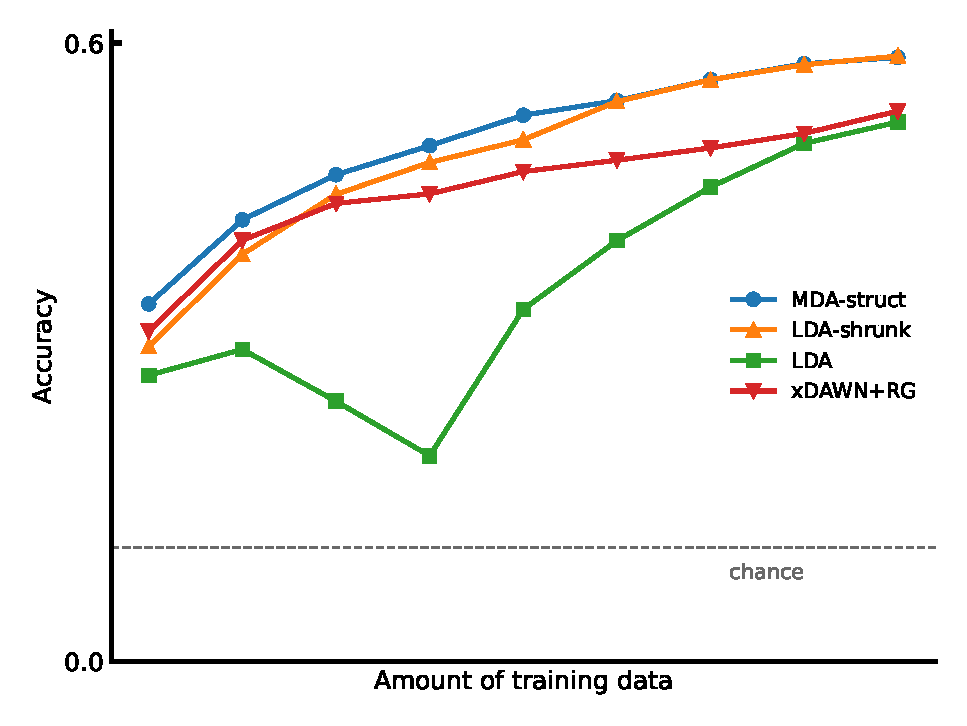
\includegraphics[width=.66\linewidth]{figures/stbf_struct/accuracy.eps}
    \sffamily
    \hspace{-0.4623567780166823in}
%% Creator: Matplotlib, PGF backend
%%
%% To include the figure in your LaTeX document, write
%%   \input{<filename>.pgf}
%%
%% Make sure the required packages are loaded in your preamble
%%   \usepackage{pgf}
%%
%% Also ensure that all the required font packages are loaded; for instance,
%% the lmodern package is sometimes necessary when using math font.
%%   \usepackage{lmodern}
%%
%% Figures using additional raster images can only be included by \input if
%% they are in the same directory as the main LaTeX file. For loading figures
%% from other directories you can use the `import` package
%%   \usepackage{import}
%%
%% and then include the figures with
%%   \import{<path to file>}{<filename>.pgf}
%%
%% Matplotlib used the following preamble
%%
\begingroup%
\makeatletter%
\begin{pgfpicture}%
\pgfpathrectangle{\pgfpointorigin}{\pgfqpoint{2.879017in}{1.916660in}}%
\pgfusepath{use as bounding box, clip}%
\begin{pgfscope}%
\pgfsetbuttcap%
\pgfsetmiterjoin%
\pgfsetlinewidth{0.000000pt}%
\definecolor{currentstroke}{rgb}{1.000000,1.000000,1.000000}%
\pgfsetstrokecolor{currentstroke}%
\pgfsetstrokeopacity{0.000000}%
\pgfsetdash{}{0pt}%
\pgfpathmoveto{\pgfqpoint{0.000000in}{0.000000in}}%
\pgfpathlineto{\pgfqpoint{2.879017in}{0.000000in}}%
\pgfpathlineto{\pgfqpoint{2.879017in}{1.916660in}}%
\pgfpathlineto{\pgfqpoint{0.000000in}{1.916660in}}%
\pgfpathlineto{\pgfqpoint{0.000000in}{0.000000in}}%
\pgfpathclose%
\pgfusepath{}%
\end{pgfscope}%
\begin{pgfscope}%
\pgfsetbuttcap%
\pgfsetmiterjoin%
\definecolor{currentfill}{rgb}{1.000000,1.000000,1.000000}%
\pgfsetfillcolor{currentfill}%
\pgfsetlinewidth{0.000000pt}%
\definecolor{currentstroke}{rgb}{0.000000,0.000000,0.000000}%
\pgfsetstrokecolor{currentstroke}%
\pgfsetstrokeopacity{0.000000}%
\pgfsetdash{}{0pt}%
\pgfpathmoveto{\pgfqpoint{0.421874in}{0.326389in}}%
\pgfpathlineto{\pgfqpoint{2.879017in}{0.326389in}}%
\pgfpathlineto{\pgfqpoint{2.879017in}{1.873257in}}%
\pgfpathlineto{\pgfqpoint{0.421874in}{1.873257in}}%
\pgfpathlineto{\pgfqpoint{0.421874in}{0.326389in}}%
\pgfpathclose%
\pgfusepath{fill}%
\end{pgfscope}%
\begin{pgfscope}%
\pgfsetbuttcap%
\pgfsetroundjoin%
\definecolor{currentfill}{rgb}{0.552941,0.501961,0.478431}%
\pgfsetfillcolor{currentfill}%
\pgfsetlinewidth{0.803000pt}%
\definecolor{currentstroke}{rgb}{0.552941,0.501961,0.478431}%
\pgfsetstrokecolor{currentstroke}%
\pgfsetdash{}{0pt}%
\pgfsys@defobject{currentmarker}{\pgfqpoint{0.000000in}{0.000000in}}{\pgfqpoint{0.000000in}{0.041667in}}{%
\pgfpathmoveto{\pgfqpoint{0.000000in}{0.000000in}}%
\pgfpathlineto{\pgfqpoint{0.000000in}{0.041667in}}%
\pgfusepath{stroke,fill}%
}%
\begin{pgfscope}%
\pgfsys@transformshift{0.812783in}{0.326389in}%
\pgfsys@useobject{currentmarker}{}%
\end{pgfscope}%
\end{pgfscope}%
\begin{pgfscope}%
\definecolor{textcolor}{rgb}{0.552941,0.501961,0.478431}%
\pgfsetstrokecolor{textcolor}%
\pgfsetfillcolor{textcolor}%
\pgftext[x=0.812783in,y=0.277778in,,top]{\color{textcolor}\sffamily\fontsize{9.000000}{10.800000}\selectfont 2}%
\end{pgfscope}%
\begin{pgfscope}%
\pgfsetbuttcap%
\pgfsetroundjoin%
\definecolor{currentfill}{rgb}{0.552941,0.501961,0.478431}%
\pgfsetfillcolor{currentfill}%
\pgfsetlinewidth{0.803000pt}%
\definecolor{currentstroke}{rgb}{0.552941,0.501961,0.478431}%
\pgfsetstrokecolor{currentstroke}%
\pgfsetdash{}{0pt}%
\pgfsys@defobject{currentmarker}{\pgfqpoint{0.000000in}{0.000000in}}{\pgfqpoint{0.000000in}{0.041667in}}{%
\pgfpathmoveto{\pgfqpoint{0.000000in}{0.000000in}}%
\pgfpathlineto{\pgfqpoint{0.000000in}{0.041667in}}%
\pgfusepath{stroke,fill}%
}%
\begin{pgfscope}%
\pgfsys@transformshift{1.371224in}{0.326389in}%
\pgfsys@useobject{currentmarker}{}%
\end{pgfscope}%
\end{pgfscope}%
\begin{pgfscope}%
\definecolor{textcolor}{rgb}{0.552941,0.501961,0.478431}%
\pgfsetstrokecolor{textcolor}%
\pgfsetfillcolor{textcolor}%
\pgftext[x=1.371224in,y=0.277778in,,top]{\color{textcolor}\sffamily\fontsize{9.000000}{10.800000}\selectfont 4}%
\end{pgfscope}%
\begin{pgfscope}%
\pgfsetbuttcap%
\pgfsetroundjoin%
\definecolor{currentfill}{rgb}{0.552941,0.501961,0.478431}%
\pgfsetfillcolor{currentfill}%
\pgfsetlinewidth{0.803000pt}%
\definecolor{currentstroke}{rgb}{0.552941,0.501961,0.478431}%
\pgfsetstrokecolor{currentstroke}%
\pgfsetdash{}{0pt}%
\pgfsys@defobject{currentmarker}{\pgfqpoint{0.000000in}{0.000000in}}{\pgfqpoint{0.000000in}{0.041667in}}{%
\pgfpathmoveto{\pgfqpoint{0.000000in}{0.000000in}}%
\pgfpathlineto{\pgfqpoint{0.000000in}{0.041667in}}%
\pgfusepath{stroke,fill}%
}%
\begin{pgfscope}%
\pgfsys@transformshift{1.929666in}{0.326389in}%
\pgfsys@useobject{currentmarker}{}%
\end{pgfscope}%
\end{pgfscope}%
\begin{pgfscope}%
\definecolor{textcolor}{rgb}{0.552941,0.501961,0.478431}%
\pgfsetstrokecolor{textcolor}%
\pgfsetfillcolor{textcolor}%
\pgftext[x=1.929666in,y=0.277778in,,top]{\color{textcolor}\sffamily\fontsize{9.000000}{10.800000}\selectfont 6}%
\end{pgfscope}%
\begin{pgfscope}%
\pgfsetbuttcap%
\pgfsetroundjoin%
\definecolor{currentfill}{rgb}{0.552941,0.501961,0.478431}%
\pgfsetfillcolor{currentfill}%
\pgfsetlinewidth{0.803000pt}%
\definecolor{currentstroke}{rgb}{0.552941,0.501961,0.478431}%
\pgfsetstrokecolor{currentstroke}%
\pgfsetdash{}{0pt}%
\pgfsys@defobject{currentmarker}{\pgfqpoint{0.000000in}{0.000000in}}{\pgfqpoint{0.000000in}{0.041667in}}{%
\pgfpathmoveto{\pgfqpoint{0.000000in}{0.000000in}}%
\pgfpathlineto{\pgfqpoint{0.000000in}{0.041667in}}%
\pgfusepath{stroke,fill}%
}%
\begin{pgfscope}%
\pgfsys@transformshift{2.488108in}{0.326389in}%
\pgfsys@useobject{currentmarker}{}%
\end{pgfscope}%
\end{pgfscope}%
\begin{pgfscope}%
\definecolor{textcolor}{rgb}{0.552941,0.501961,0.478431}%
\pgfsetstrokecolor{textcolor}%
\pgfsetfillcolor{textcolor}%
\pgftext[x=2.488108in,y=0.277778in,,top]{\color{textcolor}\sffamily\fontsize{9.000000}{10.800000}\selectfont 8}%
\end{pgfscope}%
\begin{pgfscope}%
\definecolor{textcolor}{rgb}{0.552941,0.501961,0.478431}%
\pgfsetstrokecolor{textcolor}%
\pgfsetfillcolor{textcolor}%
\pgftext[x=1.650445in,y=0.111111in,,top]{\color{textcolor}\sffamily\fontsize{9.000000}{10.800000}\selectfont Amount of training data}%
\end{pgfscope}%
\begin{pgfscope}%
\pgfsetbuttcap%
\pgfsetroundjoin%
\definecolor{currentfill}{rgb}{0.552941,0.501961,0.478431}%
\pgfsetfillcolor{currentfill}%
\pgfsetlinewidth{0.803000pt}%
\definecolor{currentstroke}{rgb}{0.552941,0.501961,0.478431}%
\pgfsetstrokecolor{currentstroke}%
\pgfsetdash{}{0pt}%
\pgfsys@defobject{currentmarker}{\pgfqpoint{0.000000in}{0.000000in}}{\pgfqpoint{0.041667in}{0.000000in}}{%
\pgfpathmoveto{\pgfqpoint{0.000000in}{0.000000in}}%
\pgfpathlineto{\pgfqpoint{0.041667in}{0.000000in}}%
\pgfusepath{stroke,fill}%
}%
\begin{pgfscope}%
\pgfsys@transformshift{0.421874in}{0.326389in}%
\pgfsys@useobject{currentmarker}{}%
\end{pgfscope}%
\end{pgfscope}%
\begin{pgfscope}%
\definecolor{textcolor}{rgb}{0.552941,0.501961,0.478431}%
\pgfsetstrokecolor{textcolor}%
\pgfsetfillcolor{textcolor}%
\pgftext[x=0.309027in, y=0.282986in, left, base]{\color{textcolor}\sffamily\fontsize{9.000000}{10.800000}\selectfont 0}%
\end{pgfscope}%
\begin{pgfscope}%
\pgfsetbuttcap%
\pgfsetroundjoin%
\definecolor{currentfill}{rgb}{0.552941,0.501961,0.478431}%
\pgfsetfillcolor{currentfill}%
\pgfsetlinewidth{0.803000pt}%
\definecolor{currentstroke}{rgb}{0.552941,0.501961,0.478431}%
\pgfsetstrokecolor{currentstroke}%
\pgfsetdash{}{0pt}%
\pgfsys@defobject{currentmarker}{\pgfqpoint{0.000000in}{0.000000in}}{\pgfqpoint{0.041667in}{0.000000in}}{%
\pgfpathmoveto{\pgfqpoint{0.000000in}{0.000000in}}%
\pgfpathlineto{\pgfqpoint{0.041667in}{0.000000in}}%
\pgfusepath{stroke,fill}%
}%
\begin{pgfscope}%
\pgfsys@transformshift{0.421874in}{0.635763in}%
\pgfsys@useobject{currentmarker}{}%
\end{pgfscope}%
\end{pgfscope}%
\begin{pgfscope}%
\definecolor{textcolor}{rgb}{0.552941,0.501961,0.478431}%
\pgfsetstrokecolor{textcolor}%
\pgfsetfillcolor{textcolor}%
\pgftext[x=0.244791in, y=0.592360in, left, base]{\color{textcolor}\sffamily\fontsize{9.000000}{10.800000}\selectfont 20}%
\end{pgfscope}%
\begin{pgfscope}%
\pgfsetbuttcap%
\pgfsetroundjoin%
\definecolor{currentfill}{rgb}{0.552941,0.501961,0.478431}%
\pgfsetfillcolor{currentfill}%
\pgfsetlinewidth{0.803000pt}%
\definecolor{currentstroke}{rgb}{0.552941,0.501961,0.478431}%
\pgfsetstrokecolor{currentstroke}%
\pgfsetdash{}{0pt}%
\pgfsys@defobject{currentmarker}{\pgfqpoint{0.000000in}{0.000000in}}{\pgfqpoint{0.041667in}{0.000000in}}{%
\pgfpathmoveto{\pgfqpoint{0.000000in}{0.000000in}}%
\pgfpathlineto{\pgfqpoint{0.041667in}{0.000000in}}%
\pgfusepath{stroke,fill}%
}%
\begin{pgfscope}%
\pgfsys@transformshift{0.421874in}{0.945136in}%
\pgfsys@useobject{currentmarker}{}%
\end{pgfscope}%
\end{pgfscope}%
\begin{pgfscope}%
\definecolor{textcolor}{rgb}{0.552941,0.501961,0.478431}%
\pgfsetstrokecolor{textcolor}%
\pgfsetfillcolor{textcolor}%
\pgftext[x=0.244791in, y=0.901733in, left, base]{\color{textcolor}\sffamily\fontsize{9.000000}{10.800000}\selectfont 40}%
\end{pgfscope}%
\begin{pgfscope}%
\pgfsetbuttcap%
\pgfsetroundjoin%
\definecolor{currentfill}{rgb}{0.552941,0.501961,0.478431}%
\pgfsetfillcolor{currentfill}%
\pgfsetlinewidth{0.803000pt}%
\definecolor{currentstroke}{rgb}{0.552941,0.501961,0.478431}%
\pgfsetstrokecolor{currentstroke}%
\pgfsetdash{}{0pt}%
\pgfsys@defobject{currentmarker}{\pgfqpoint{0.000000in}{0.000000in}}{\pgfqpoint{0.041667in}{0.000000in}}{%
\pgfpathmoveto{\pgfqpoint{0.000000in}{0.000000in}}%
\pgfpathlineto{\pgfqpoint{0.041667in}{0.000000in}}%
\pgfusepath{stroke,fill}%
}%
\begin{pgfscope}%
\pgfsys@transformshift{0.421874in}{1.254510in}%
\pgfsys@useobject{currentmarker}{}%
\end{pgfscope}%
\end{pgfscope}%
\begin{pgfscope}%
\definecolor{textcolor}{rgb}{0.552941,0.501961,0.478431}%
\pgfsetstrokecolor{textcolor}%
\pgfsetfillcolor{textcolor}%
\pgftext[x=0.244791in, y=1.211107in, left, base]{\color{textcolor}\sffamily\fontsize{9.000000}{10.800000}\selectfont 60}%
\end{pgfscope}%
\begin{pgfscope}%
\pgfsetbuttcap%
\pgfsetroundjoin%
\definecolor{currentfill}{rgb}{0.552941,0.501961,0.478431}%
\pgfsetfillcolor{currentfill}%
\pgfsetlinewidth{0.803000pt}%
\definecolor{currentstroke}{rgb}{0.552941,0.501961,0.478431}%
\pgfsetstrokecolor{currentstroke}%
\pgfsetdash{}{0pt}%
\pgfsys@defobject{currentmarker}{\pgfqpoint{0.000000in}{0.000000in}}{\pgfqpoint{0.041667in}{0.000000in}}{%
\pgfpathmoveto{\pgfqpoint{0.000000in}{0.000000in}}%
\pgfpathlineto{\pgfqpoint{0.041667in}{0.000000in}}%
\pgfusepath{stroke,fill}%
}%
\begin{pgfscope}%
\pgfsys@transformshift{0.421874in}{1.563884in}%
\pgfsys@useobject{currentmarker}{}%
\end{pgfscope}%
\end{pgfscope}%
\begin{pgfscope}%
\definecolor{textcolor}{rgb}{0.552941,0.501961,0.478431}%
\pgfsetstrokecolor{textcolor}%
\pgfsetfillcolor{textcolor}%
\pgftext[x=0.244791in, y=1.520481in, left, base]{\color{textcolor}\sffamily\fontsize{9.000000}{10.800000}\selectfont 80}%
\end{pgfscope}%
\begin{pgfscope}%
\pgfsetbuttcap%
\pgfsetroundjoin%
\definecolor{currentfill}{rgb}{0.552941,0.501961,0.478431}%
\pgfsetfillcolor{currentfill}%
\pgfsetlinewidth{0.803000pt}%
\definecolor{currentstroke}{rgb}{0.552941,0.501961,0.478431}%
\pgfsetstrokecolor{currentstroke}%
\pgfsetdash{}{0pt}%
\pgfsys@defobject{currentmarker}{\pgfqpoint{0.000000in}{0.000000in}}{\pgfqpoint{0.041667in}{0.000000in}}{%
\pgfpathmoveto{\pgfqpoint{0.000000in}{0.000000in}}%
\pgfpathlineto{\pgfqpoint{0.041667in}{0.000000in}}%
\pgfusepath{stroke,fill}%
}%
\begin{pgfscope}%
\pgfsys@transformshift{0.421874in}{1.873257in}%
\pgfsys@useobject{currentmarker}{}%
\end{pgfscope}%
\end{pgfscope}%
\begin{pgfscope}%
\definecolor{textcolor}{rgb}{0.552941,0.501961,0.478431}%
\pgfsetstrokecolor{textcolor}%
\pgfsetfillcolor{textcolor}%
\pgftext[x=0.180556in, y=1.829854in, left, base]{\color{textcolor}\sffamily\fontsize{9.000000}{10.800000}\selectfont 100}%
\end{pgfscope}%
\begin{pgfscope}%
\definecolor{textcolor}{rgb}{0.552941,0.501961,0.478431}%
\pgfsetstrokecolor{textcolor}%
\pgfsetfillcolor{textcolor}%
\pgftext[x=0.125000in,y=1.099823in,,bottom,rotate=90.000000]{\color{textcolor}\sffamily\fontsize{9.000000}{10.800000}\selectfont Accuracy (\%)}%
\end{pgfscope}%
\begin{pgfscope}%
\pgfpathrectangle{\pgfqpoint{0.421874in}{0.326389in}}{\pgfqpoint{2.457143in}{1.546868in}}%
\pgfusepath{clip}%
\pgfsetrectcap%
\pgfsetroundjoin%
\pgfsetlinewidth{1.505625pt}%
\definecolor{currentstroke}{rgb}{0.949020,0.564706,0.094118}%
\pgfsetstrokecolor{currentstroke}%
\pgfsetdash{}{0pt}%
\pgfpathmoveto{\pgfqpoint{0.533562in}{0.863155in}}%
\pgfpathlineto{\pgfqpoint{0.812783in}{0.989332in}}%
\pgfpathlineto{\pgfqpoint{1.092004in}{1.056854in}}%
\pgfpathlineto{\pgfqpoint{1.371224in}{1.100505in}}%
\pgfpathlineto{\pgfqpoint{1.650445in}{1.146202in}}%
\pgfpathlineto{\pgfqpoint{1.929666in}{1.168027in}}%
\pgfpathlineto{\pgfqpoint{2.208887in}{1.199401in}}%
\pgfpathlineto{\pgfqpoint{2.488108in}{1.223272in}}%
\pgfpathlineto{\pgfqpoint{2.767328in}{1.232821in}}%
\pgfusepath{stroke}%
\end{pgfscope}%
\begin{pgfscope}%
\pgfpathrectangle{\pgfqpoint{0.421874in}{0.326389in}}{\pgfqpoint{2.457143in}{1.546868in}}%
\pgfusepath{clip}%
\pgfsetbuttcap%
\pgfsetmiterjoin%
\definecolor{currentfill}{rgb}{0.949020,0.564706,0.094118}%
\pgfsetfillcolor{currentfill}%
\pgfsetlinewidth{0.000000pt}%
\definecolor{currentstroke}{rgb}{1.000000,1.000000,1.000000}%
\pgfsetstrokecolor{currentstroke}%
\pgfsetdash{}{0pt}%
\pgfsys@defobject{currentmarker}{\pgfqpoint{-0.020833in}{-0.020833in}}{\pgfqpoint{0.020833in}{0.020833in}}{%
\pgfpathmoveto{\pgfqpoint{-0.020833in}{-0.020833in}}%
\pgfpathlineto{\pgfqpoint{0.020833in}{-0.020833in}}%
\pgfpathlineto{\pgfqpoint{0.020833in}{0.020833in}}%
\pgfpathlineto{\pgfqpoint{-0.020833in}{0.020833in}}%
\pgfpathlineto{\pgfqpoint{-0.020833in}{-0.020833in}}%
\pgfpathclose%
\pgfusepath{fill}%
}%
\begin{pgfscope}%
\pgfsys@transformshift{0.533562in}{0.863155in}%
\pgfsys@useobject{currentmarker}{}%
\end{pgfscope}%
\begin{pgfscope}%
\pgfsys@transformshift{0.812783in}{0.989332in}%
\pgfsys@useobject{currentmarker}{}%
\end{pgfscope}%
\begin{pgfscope}%
\pgfsys@transformshift{1.092004in}{1.056854in}%
\pgfsys@useobject{currentmarker}{}%
\end{pgfscope}%
\begin{pgfscope}%
\pgfsys@transformshift{1.371224in}{1.100505in}%
\pgfsys@useobject{currentmarker}{}%
\end{pgfscope}%
\begin{pgfscope}%
\pgfsys@transformshift{1.650445in}{1.146202in}%
\pgfsys@useobject{currentmarker}{}%
\end{pgfscope}%
\begin{pgfscope}%
\pgfsys@transformshift{1.929666in}{1.168027in}%
\pgfsys@useobject{currentmarker}{}%
\end{pgfscope}%
\begin{pgfscope}%
\pgfsys@transformshift{2.208887in}{1.199401in}%
\pgfsys@useobject{currentmarker}{}%
\end{pgfscope}%
\begin{pgfscope}%
\pgfsys@transformshift{2.488108in}{1.223272in}%
\pgfsys@useobject{currentmarker}{}%
\end{pgfscope}%
\begin{pgfscope}%
\pgfsys@transformshift{2.767328in}{1.232821in}%
\pgfsys@useobject{currentmarker}{}%
\end{pgfscope}%
\end{pgfscope}%
\begin{pgfscope}%
\pgfpathrectangle{\pgfqpoint{0.421874in}{0.326389in}}{\pgfqpoint{2.457143in}{1.546868in}}%
\pgfusepath{clip}%
\pgfsetrectcap%
\pgfsetroundjoin%
\pgfsetlinewidth{1.505625pt}%
\definecolor{currentstroke}{rgb}{0.964706,0.239216,0.117647}%
\pgfsetstrokecolor{currentstroke}%
\pgfsetdash{}{0pt}%
\pgfpathmoveto{\pgfqpoint{0.533562in}{0.799043in}}%
\pgfpathlineto{\pgfqpoint{0.812783in}{0.937497in}}%
\pgfpathlineto{\pgfqpoint{1.092004in}{1.027527in}}%
\pgfpathlineto{\pgfqpoint{1.371224in}{1.075270in}}%
\pgfpathlineto{\pgfqpoint{1.650445in}{1.109372in}}%
\pgfpathlineto{\pgfqpoint{1.929666in}{1.166663in}}%
\pgfpathlineto{\pgfqpoint{2.208887in}{1.199401in}}%
\pgfpathlineto{\pgfqpoint{2.488108in}{1.221908in}}%
\pgfpathlineto{\pgfqpoint{2.767328in}{1.234867in}}%
\pgfusepath{stroke}%
\end{pgfscope}%
\begin{pgfscope}%
\pgfpathrectangle{\pgfqpoint{0.421874in}{0.326389in}}{\pgfqpoint{2.457143in}{1.546868in}}%
\pgfusepath{clip}%
\pgfsetbuttcap%
\pgfsetmiterjoin%
\definecolor{currentfill}{rgb}{0.964706,0.239216,0.117647}%
\pgfsetfillcolor{currentfill}%
\pgfsetlinewidth{0.000000pt}%
\definecolor{currentstroke}{rgb}{1.000000,1.000000,1.000000}%
\pgfsetstrokecolor{currentstroke}%
\pgfsetdash{}{0pt}%
\pgfsys@defobject{currentmarker}{\pgfqpoint{-0.029463in}{-0.029463in}}{\pgfqpoint{0.029463in}{0.029463in}}{%
\pgfpathmoveto{\pgfqpoint{-0.000000in}{-0.029463in}}%
\pgfpathlineto{\pgfqpoint{0.029463in}{0.000000in}}%
\pgfpathlineto{\pgfqpoint{0.000000in}{0.029463in}}%
\pgfpathlineto{\pgfqpoint{-0.029463in}{0.000000in}}%
\pgfpathlineto{\pgfqpoint{-0.000000in}{-0.029463in}}%
\pgfpathclose%
\pgfusepath{fill}%
}%
\begin{pgfscope}%
\pgfsys@transformshift{0.533562in}{0.799043in}%
\pgfsys@useobject{currentmarker}{}%
\end{pgfscope}%
\begin{pgfscope}%
\pgfsys@transformshift{0.812783in}{0.937497in}%
\pgfsys@useobject{currentmarker}{}%
\end{pgfscope}%
\begin{pgfscope}%
\pgfsys@transformshift{1.092004in}{1.027527in}%
\pgfsys@useobject{currentmarker}{}%
\end{pgfscope}%
\begin{pgfscope}%
\pgfsys@transformshift{1.371224in}{1.075270in}%
\pgfsys@useobject{currentmarker}{}%
\end{pgfscope}%
\begin{pgfscope}%
\pgfsys@transformshift{1.650445in}{1.109372in}%
\pgfsys@useobject{currentmarker}{}%
\end{pgfscope}%
\begin{pgfscope}%
\pgfsys@transformshift{1.929666in}{1.166663in}%
\pgfsys@useobject{currentmarker}{}%
\end{pgfscope}%
\begin{pgfscope}%
\pgfsys@transformshift{2.208887in}{1.199401in}%
\pgfsys@useobject{currentmarker}{}%
\end{pgfscope}%
\begin{pgfscope}%
\pgfsys@transformshift{2.488108in}{1.221908in}%
\pgfsys@useobject{currentmarker}{}%
\end{pgfscope}%
\begin{pgfscope}%
\pgfsys@transformshift{2.767328in}{1.234867in}%
\pgfsys@useobject{currentmarker}{}%
\end{pgfscope}%
\end{pgfscope}%
\begin{pgfscope}%
\pgfpathrectangle{\pgfqpoint{0.421874in}{0.326389in}}{\pgfqpoint{2.457143in}{1.546868in}}%
\pgfusepath{clip}%
\pgfsetrectcap%
\pgfsetroundjoin%
\pgfsetlinewidth{1.505625pt}%
\definecolor{currentstroke}{rgb}{0.470588,0.278431,0.615686}%
\pgfsetstrokecolor{currentstroke}%
\pgfsetdash{}{0pt}%
\pgfpathmoveto{\pgfqpoint{0.533562in}{0.756075in}}%
\pgfpathlineto{\pgfqpoint{0.812783in}{0.794951in}}%
\pgfpathlineto{\pgfqpoint{1.092004in}{0.717198in}}%
\pgfpathlineto{\pgfqpoint{1.371224in}{0.635353in}}%
\pgfpathlineto{\pgfqpoint{1.650445in}{0.854970in}}%
\pgfpathlineto{\pgfqpoint{1.929666in}{0.957959in}}%
\pgfpathlineto{\pgfqpoint{2.208887in}{1.038439in}}%
\pgfpathlineto{\pgfqpoint{2.488108in}{1.103915in}}%
\pgfpathlineto{\pgfqpoint{2.767328in}{1.135971in}}%
\pgfusepath{stroke}%
\end{pgfscope}%
\begin{pgfscope}%
\pgfpathrectangle{\pgfqpoint{0.421874in}{0.326389in}}{\pgfqpoint{2.457143in}{1.546868in}}%
\pgfusepath{clip}%
\pgfsetbuttcap%
\pgfsetroundjoin%
\definecolor{currentfill}{rgb}{0.470588,0.278431,0.615686}%
\pgfsetfillcolor{currentfill}%
\pgfsetlinewidth{0.000000pt}%
\definecolor{currentstroke}{rgb}{1.000000,1.000000,1.000000}%
\pgfsetstrokecolor{currentstroke}%
\pgfsetdash{}{0pt}%
\pgfsys@defobject{currentmarker}{\pgfqpoint{-0.020833in}{-0.020833in}}{\pgfqpoint{0.020833in}{0.020833in}}{%
\pgfpathmoveto{\pgfqpoint{0.000000in}{-0.020833in}}%
\pgfpathcurveto{\pgfqpoint{0.005525in}{-0.020833in}}{\pgfqpoint{0.010825in}{-0.018638in}}{\pgfqpoint{0.014731in}{-0.014731in}}%
\pgfpathcurveto{\pgfqpoint{0.018638in}{-0.010825in}}{\pgfqpoint{0.020833in}{-0.005525in}}{\pgfqpoint{0.020833in}{0.000000in}}%
\pgfpathcurveto{\pgfqpoint{0.020833in}{0.005525in}}{\pgfqpoint{0.018638in}{0.010825in}}{\pgfqpoint{0.014731in}{0.014731in}}%
\pgfpathcurveto{\pgfqpoint{0.010825in}{0.018638in}}{\pgfqpoint{0.005525in}{0.020833in}}{\pgfqpoint{0.000000in}{0.020833in}}%
\pgfpathcurveto{\pgfqpoint{-0.005525in}{0.020833in}}{\pgfqpoint{-0.010825in}{0.018638in}}{\pgfqpoint{-0.014731in}{0.014731in}}%
\pgfpathcurveto{\pgfqpoint{-0.018638in}{0.010825in}}{\pgfqpoint{-0.020833in}{0.005525in}}{\pgfqpoint{-0.020833in}{0.000000in}}%
\pgfpathcurveto{\pgfqpoint{-0.020833in}{-0.005525in}}{\pgfqpoint{-0.018638in}{-0.010825in}}{\pgfqpoint{-0.014731in}{-0.014731in}}%
\pgfpathcurveto{\pgfqpoint{-0.010825in}{-0.018638in}}{\pgfqpoint{-0.005525in}{-0.020833in}}{\pgfqpoint{0.000000in}{-0.020833in}}%
\pgfpathlineto{\pgfqpoint{0.000000in}{-0.020833in}}%
\pgfpathclose%
\pgfusepath{fill}%
}%
\begin{pgfscope}%
\pgfsys@transformshift{0.533562in}{0.756075in}%
\pgfsys@useobject{currentmarker}{}%
\end{pgfscope}%
\begin{pgfscope}%
\pgfsys@transformshift{0.812783in}{0.794951in}%
\pgfsys@useobject{currentmarker}{}%
\end{pgfscope}%
\begin{pgfscope}%
\pgfsys@transformshift{1.092004in}{0.717198in}%
\pgfsys@useobject{currentmarker}{}%
\end{pgfscope}%
\begin{pgfscope}%
\pgfsys@transformshift{1.371224in}{0.635353in}%
\pgfsys@useobject{currentmarker}{}%
\end{pgfscope}%
\begin{pgfscope}%
\pgfsys@transformshift{1.650445in}{0.854970in}%
\pgfsys@useobject{currentmarker}{}%
\end{pgfscope}%
\begin{pgfscope}%
\pgfsys@transformshift{1.929666in}{0.957959in}%
\pgfsys@useobject{currentmarker}{}%
\end{pgfscope}%
\begin{pgfscope}%
\pgfsys@transformshift{2.208887in}{1.038439in}%
\pgfsys@useobject{currentmarker}{}%
\end{pgfscope}%
\begin{pgfscope}%
\pgfsys@transformshift{2.488108in}{1.103915in}%
\pgfsys@useobject{currentmarker}{}%
\end{pgfscope}%
\begin{pgfscope}%
\pgfsys@transformshift{2.767328in}{1.135971in}%
\pgfsys@useobject{currentmarker}{}%
\end{pgfscope}%
\end{pgfscope}%
\begin{pgfscope}%
\pgfpathrectangle{\pgfqpoint{0.421874in}{0.326389in}}{\pgfqpoint{2.457143in}{1.546868in}}%
\pgfusepath{clip}%
\pgfsetrectcap%
\pgfsetroundjoin%
\pgfsetlinewidth{1.505625pt}%
\definecolor{currentstroke}{rgb}{0.454902,0.643137,0.737255}%
\pgfsetstrokecolor{currentstroke}%
\pgfsetdash{}{0pt}%
\pgfpathmoveto{\pgfqpoint{0.533562in}{0.822232in}}%
\pgfpathlineto{\pgfqpoint{0.812783in}{0.958641in}}%
\pgfpathlineto{\pgfqpoint{1.092004in}{1.013886in}}%
\pgfpathlineto{\pgfqpoint{1.371224in}{1.028209in}}%
\pgfpathlineto{\pgfqpoint{1.650445in}{1.061629in}}%
\pgfpathlineto{\pgfqpoint{1.929666in}{1.078680in}}%
\pgfpathlineto{\pgfqpoint{2.208887in}{1.097095in}}%
\pgfpathlineto{\pgfqpoint{2.488108in}{1.118920in}}%
\pgfpathlineto{\pgfqpoint{2.767328in}{1.152340in}}%
\pgfusepath{stroke}%
\end{pgfscope}%
\begin{pgfscope}%
\pgfpathrectangle{\pgfqpoint{0.421874in}{0.326389in}}{\pgfqpoint{2.457143in}{1.546868in}}%
\pgfusepath{clip}%
\pgfsetbuttcap%
\pgfsetmiterjoin%
\definecolor{currentfill}{rgb}{0.454902,0.643137,0.737255}%
\pgfsetfillcolor{currentfill}%
\pgfsetlinewidth{0.000000pt}%
\definecolor{currentstroke}{rgb}{1.000000,1.000000,1.000000}%
\pgfsetstrokecolor{currentstroke}%
\pgfsetdash{}{0pt}%
\pgfsys@defobject{currentmarker}{\pgfqpoint{-0.020833in}{-0.020833in}}{\pgfqpoint{0.020833in}{0.020833in}}{%
\pgfpathmoveto{\pgfqpoint{-0.006944in}{-0.020833in}}%
\pgfpathlineto{\pgfqpoint{0.006944in}{-0.020833in}}%
\pgfpathlineto{\pgfqpoint{0.006944in}{-0.006944in}}%
\pgfpathlineto{\pgfqpoint{0.020833in}{-0.006944in}}%
\pgfpathlineto{\pgfqpoint{0.020833in}{0.006944in}}%
\pgfpathlineto{\pgfqpoint{0.006944in}{0.006944in}}%
\pgfpathlineto{\pgfqpoint{0.006944in}{0.020833in}}%
\pgfpathlineto{\pgfqpoint{-0.006944in}{0.020833in}}%
\pgfpathlineto{\pgfqpoint{-0.006944in}{0.006944in}}%
\pgfpathlineto{\pgfqpoint{-0.020833in}{0.006944in}}%
\pgfpathlineto{\pgfqpoint{-0.020833in}{-0.006944in}}%
\pgfpathlineto{\pgfqpoint{-0.006944in}{-0.006944in}}%
\pgfpathlineto{\pgfqpoint{-0.006944in}{-0.020833in}}%
\pgfpathclose%
\pgfusepath{fill}%
}%
\begin{pgfscope}%
\pgfsys@transformshift{0.533562in}{0.822232in}%
\pgfsys@useobject{currentmarker}{}%
\end{pgfscope}%
\begin{pgfscope}%
\pgfsys@transformshift{0.812783in}{0.958641in}%
\pgfsys@useobject{currentmarker}{}%
\end{pgfscope}%
\begin{pgfscope}%
\pgfsys@transformshift{1.092004in}{1.013886in}%
\pgfsys@useobject{currentmarker}{}%
\end{pgfscope}%
\begin{pgfscope}%
\pgfsys@transformshift{1.371224in}{1.028209in}%
\pgfsys@useobject{currentmarker}{}%
\end{pgfscope}%
\begin{pgfscope}%
\pgfsys@transformshift{1.650445in}{1.061629in}%
\pgfsys@useobject{currentmarker}{}%
\end{pgfscope}%
\begin{pgfscope}%
\pgfsys@transformshift{1.929666in}{1.078680in}%
\pgfsys@useobject{currentmarker}{}%
\end{pgfscope}%
\begin{pgfscope}%
\pgfsys@transformshift{2.208887in}{1.097095in}%
\pgfsys@useobject{currentmarker}{}%
\end{pgfscope}%
\begin{pgfscope}%
\pgfsys@transformshift{2.488108in}{1.118920in}%
\pgfsys@useobject{currentmarker}{}%
\end{pgfscope}%
\begin{pgfscope}%
\pgfsys@transformshift{2.767328in}{1.152340in}%
\pgfsys@useobject{currentmarker}{}%
\end{pgfscope}%
\end{pgfscope}%
\begin{pgfscope}%
\pgfpathrectangle{\pgfqpoint{0.421874in}{0.326389in}}{\pgfqpoint{2.457143in}{1.546868in}}%
\pgfusepath{clip}%
\pgfsetbuttcap%
\pgfsetroundjoin%
\pgfsetlinewidth{1.003750pt}%
\definecolor{currentstroke}{rgb}{0.878431,0.878431,0.878431}%
\pgfsetstrokecolor{currentstroke}%
\pgfsetdash{{3.700000pt}{1.600000pt}}{0.000000pt}%
\pgfpathmoveto{\pgfqpoint{0.421874in}{0.498263in}}%
\pgfpathlineto{\pgfqpoint{2.879017in}{0.498263in}}%
\pgfusepath{stroke}%
\end{pgfscope}%
\begin{pgfscope}%
\pgfsetrectcap%
\pgfsetmiterjoin%
\pgfsetlinewidth{0.803000pt}%
\definecolor{currentstroke}{rgb}{0.552941,0.501961,0.478431}%
\pgfsetstrokecolor{currentstroke}%
\pgfsetdash{}{0pt}%
\pgfpathmoveto{\pgfqpoint{0.421874in}{0.326389in}}%
\pgfpathlineto{\pgfqpoint{0.421874in}{1.873257in}}%
\pgfusepath{stroke}%
\end{pgfscope}%
\begin{pgfscope}%
\pgfsetrectcap%
\pgfsetmiterjoin%
\pgfsetlinewidth{0.803000pt}%
\definecolor{currentstroke}{rgb}{0.552941,0.501961,0.478431}%
\pgfsetstrokecolor{currentstroke}%
\pgfsetdash{}{0pt}%
\pgfpathmoveto{\pgfqpoint{2.879017in}{0.326389in}}%
\pgfpathlineto{\pgfqpoint{2.879017in}{1.873257in}}%
\pgfusepath{stroke}%
\end{pgfscope}%
\begin{pgfscope}%
\pgfsetrectcap%
\pgfsetmiterjoin%
\pgfsetlinewidth{0.803000pt}%
\definecolor{currentstroke}{rgb}{0.552941,0.501961,0.478431}%
\pgfsetstrokecolor{currentstroke}%
\pgfsetdash{}{0pt}%
\pgfpathmoveto{\pgfqpoint{0.421874in}{0.326389in}}%
\pgfpathlineto{\pgfqpoint{2.879017in}{0.326389in}}%
\pgfusepath{stroke}%
\end{pgfscope}%
\begin{pgfscope}%
\pgfsetrectcap%
\pgfsetmiterjoin%
\pgfsetlinewidth{0.803000pt}%
\definecolor{currentstroke}{rgb}{0.552941,0.501961,0.478431}%
\pgfsetstrokecolor{currentstroke}%
\pgfsetdash{}{0pt}%
\pgfpathmoveto{\pgfqpoint{0.421874in}{1.873257in}}%
\pgfpathlineto{\pgfqpoint{2.879017in}{1.873257in}}%
\pgfusepath{stroke}%
\end{pgfscope}%
\begin{pgfscope}%
\pgfsetbuttcap%
\pgfsetmiterjoin%
\definecolor{currentfill}{rgb}{1.000000,1.000000,1.000000}%
\pgfsetfillcolor{currentfill}%
\pgfsetlinewidth{0.000000pt}%
\definecolor{currentstroke}{rgb}{0.000000,0.000000,0.000000}%
\pgfsetstrokecolor{currentstroke}%
\pgfsetdash{}{0pt}%
\pgfpathmoveto{\pgfqpoint{0.544731in}{0.532638in}}%
\pgfpathlineto{\pgfqpoint{0.910469in}{0.532638in}}%
\pgfpathlineto{\pgfqpoint{0.910469in}{0.643749in}}%
\pgfpathlineto{\pgfqpoint{0.544731in}{0.643749in}}%
\pgfpathlineto{\pgfqpoint{0.544731in}{0.532638in}}%
\pgfpathclose%
\pgfusepath{fill}%
\end{pgfscope}%
\begin{pgfscope}%
\definecolor{textcolor}{rgb}{0.552941,0.501961,0.478431}%
\pgfsetstrokecolor{textcolor}%
\pgfsetfillcolor{textcolor}%
\pgftext[x=0.544731in,y=0.532638in,left,bottom]{\color{textcolor}\sffamily\fontsize{9.000000}{10.800000}\selectfont chance}%
\end{pgfscope}%
\begin{pgfscope}%
\pgfsetbuttcap%
\pgfsetmiterjoin%
\pgfsetlinewidth{0.000000pt}%
\definecolor{currentstroke}{rgb}{0.000000,0.000000,0.000000}%
\pgfsetstrokecolor{currentstroke}%
\pgfsetstrokeopacity{0.000000}%
\pgfsetdash{}{0pt}%
\pgfpathmoveto{\pgfqpoint{0.509374in}{1.097641in}}%
\pgfpathlineto{\pgfqpoint{1.493896in}{1.097641in}}%
\pgfpathquadraticcurveto{\pgfqpoint{1.518896in}{1.097641in}}{\pgfqpoint{1.518896in}{1.122641in}}%
\pgfpathlineto{\pgfqpoint{1.518896in}{1.785757in}}%
\pgfpathquadraticcurveto{\pgfqpoint{1.518896in}{1.810757in}}{\pgfqpoint{1.493896in}{1.810757in}}%
\pgfpathlineto{\pgfqpoint{0.509374in}{1.810757in}}%
\pgfpathquadraticcurveto{\pgfqpoint{0.484374in}{1.810757in}}{\pgfqpoint{0.484374in}{1.785757in}}%
\pgfpathlineto{\pgfqpoint{0.484374in}{1.122641in}}%
\pgfpathquadraticcurveto{\pgfqpoint{0.484374in}{1.097641in}}{\pgfqpoint{0.509374in}{1.097641in}}%
\pgfpathlineto{\pgfqpoint{0.509374in}{1.097641in}}%
\pgfpathclose%
\pgfusepath{}%
\end{pgfscope}%
\begin{pgfscope}%
\pgfsetrectcap%
\pgfsetroundjoin%
\pgfsetlinewidth{1.505625pt}%
\definecolor{currentstroke}{rgb}{0.949020,0.564706,0.094118}%
\pgfsetstrokecolor{currentstroke}%
\pgfsetdash{}{0pt}%
\pgfpathmoveto{\pgfqpoint{0.534374in}{1.717007in}}%
\pgfpathlineto{\pgfqpoint{0.659374in}{1.717007in}}%
\pgfpathlineto{\pgfqpoint{0.784374in}{1.717007in}}%
\pgfusepath{stroke}%
\end{pgfscope}%
\begin{pgfscope}%
\pgfsetbuttcap%
\pgfsetmiterjoin%
\definecolor{currentfill}{rgb}{0.949020,0.564706,0.094118}%
\pgfsetfillcolor{currentfill}%
\pgfsetlinewidth{0.000000pt}%
\definecolor{currentstroke}{rgb}{1.000000,1.000000,1.000000}%
\pgfsetstrokecolor{currentstroke}%
\pgfsetdash{}{0pt}%
\pgfsys@defobject{currentmarker}{\pgfqpoint{-0.020833in}{-0.020833in}}{\pgfqpoint{0.020833in}{0.020833in}}{%
\pgfpathmoveto{\pgfqpoint{-0.020833in}{-0.020833in}}%
\pgfpathlineto{\pgfqpoint{0.020833in}{-0.020833in}}%
\pgfpathlineto{\pgfqpoint{0.020833in}{0.020833in}}%
\pgfpathlineto{\pgfqpoint{-0.020833in}{0.020833in}}%
\pgfpathlineto{\pgfqpoint{-0.020833in}{-0.020833in}}%
\pgfpathclose%
\pgfusepath{fill}%
}%
\begin{pgfscope}%
\pgfsys@transformshift{0.659374in}{1.717007in}%
\pgfsys@useobject{currentmarker}{}%
\end{pgfscope}%
\end{pgfscope}%
\begin{pgfscope}%
\definecolor{textcolor}{rgb}{0.552941,0.501961,0.478431}%
\pgfsetstrokecolor{textcolor}%
\pgfsetfillcolor{textcolor}%
\pgftext[x=0.884374in,y=1.673257in,left,base]{\color{textcolor}\sffamily\fontsize{7.000000}{8.400000}\selectfont STBF-struct}%
\end{pgfscope}%
\begin{pgfscope}%
\pgfsetrectcap%
\pgfsetroundjoin%
\pgfsetlinewidth{1.505625pt}%
\definecolor{currentstroke}{rgb}{0.964706,0.239216,0.117647}%
\pgfsetstrokecolor{currentstroke}%
\pgfsetdash{}{0pt}%
\pgfpathmoveto{\pgfqpoint{0.534374in}{1.548103in}}%
\pgfpathlineto{\pgfqpoint{0.659374in}{1.548103in}}%
\pgfpathlineto{\pgfqpoint{0.784374in}{1.548103in}}%
\pgfusepath{stroke}%
\end{pgfscope}%
\begin{pgfscope}%
\pgfsetbuttcap%
\pgfsetmiterjoin%
\definecolor{currentfill}{rgb}{0.964706,0.239216,0.117647}%
\pgfsetfillcolor{currentfill}%
\pgfsetlinewidth{0.000000pt}%
\definecolor{currentstroke}{rgb}{1.000000,1.000000,1.000000}%
\pgfsetstrokecolor{currentstroke}%
\pgfsetdash{}{0pt}%
\pgfsys@defobject{currentmarker}{\pgfqpoint{-0.029463in}{-0.029463in}}{\pgfqpoint{0.029463in}{0.029463in}}{%
\pgfpathmoveto{\pgfqpoint{-0.000000in}{-0.029463in}}%
\pgfpathlineto{\pgfqpoint{0.029463in}{0.000000in}}%
\pgfpathlineto{\pgfqpoint{0.000000in}{0.029463in}}%
\pgfpathlineto{\pgfqpoint{-0.029463in}{0.000000in}}%
\pgfpathlineto{\pgfqpoint{-0.000000in}{-0.029463in}}%
\pgfpathclose%
\pgfusepath{fill}%
}%
\begin{pgfscope}%
\pgfsys@transformshift{0.659374in}{1.548103in}%
\pgfsys@useobject{currentmarker}{}%
\end{pgfscope}%
\end{pgfscope}%
\begin{pgfscope}%
\definecolor{textcolor}{rgb}{0.552941,0.501961,0.478431}%
\pgfsetstrokecolor{textcolor}%
\pgfsetfillcolor{textcolor}%
\pgftext[x=0.884374in,y=1.504353in,left,base]{\color{textcolor}\sffamily\fontsize{7.000000}{8.400000}\selectfont STBF-shrunk}%
\end{pgfscope}%
\begin{pgfscope}%
\pgfsetrectcap%
\pgfsetroundjoin%
\pgfsetlinewidth{1.505625pt}%
\definecolor{currentstroke}{rgb}{0.470588,0.278431,0.615686}%
\pgfsetstrokecolor{currentstroke}%
\pgfsetdash{}{0pt}%
\pgfpathmoveto{\pgfqpoint{0.534374in}{1.379199in}}%
\pgfpathlineto{\pgfqpoint{0.659374in}{1.379199in}}%
\pgfpathlineto{\pgfqpoint{0.784374in}{1.379199in}}%
\pgfusepath{stroke}%
\end{pgfscope}%
\begin{pgfscope}%
\pgfsetbuttcap%
\pgfsetroundjoin%
\definecolor{currentfill}{rgb}{0.470588,0.278431,0.615686}%
\pgfsetfillcolor{currentfill}%
\pgfsetlinewidth{0.000000pt}%
\definecolor{currentstroke}{rgb}{1.000000,1.000000,1.000000}%
\pgfsetstrokecolor{currentstroke}%
\pgfsetdash{}{0pt}%
\pgfsys@defobject{currentmarker}{\pgfqpoint{-0.020833in}{-0.020833in}}{\pgfqpoint{0.020833in}{0.020833in}}{%
\pgfpathmoveto{\pgfqpoint{0.000000in}{-0.020833in}}%
\pgfpathcurveto{\pgfqpoint{0.005525in}{-0.020833in}}{\pgfqpoint{0.010825in}{-0.018638in}}{\pgfqpoint{0.014731in}{-0.014731in}}%
\pgfpathcurveto{\pgfqpoint{0.018638in}{-0.010825in}}{\pgfqpoint{0.020833in}{-0.005525in}}{\pgfqpoint{0.020833in}{0.000000in}}%
\pgfpathcurveto{\pgfqpoint{0.020833in}{0.005525in}}{\pgfqpoint{0.018638in}{0.010825in}}{\pgfqpoint{0.014731in}{0.014731in}}%
\pgfpathcurveto{\pgfqpoint{0.010825in}{0.018638in}}{\pgfqpoint{0.005525in}{0.020833in}}{\pgfqpoint{0.000000in}{0.020833in}}%
\pgfpathcurveto{\pgfqpoint{-0.005525in}{0.020833in}}{\pgfqpoint{-0.010825in}{0.018638in}}{\pgfqpoint{-0.014731in}{0.014731in}}%
\pgfpathcurveto{\pgfqpoint{-0.018638in}{0.010825in}}{\pgfqpoint{-0.020833in}{0.005525in}}{\pgfqpoint{-0.020833in}{0.000000in}}%
\pgfpathcurveto{\pgfqpoint{-0.020833in}{-0.005525in}}{\pgfqpoint{-0.018638in}{-0.010825in}}{\pgfqpoint{-0.014731in}{-0.014731in}}%
\pgfpathcurveto{\pgfqpoint{-0.010825in}{-0.018638in}}{\pgfqpoint{-0.005525in}{-0.020833in}}{\pgfqpoint{0.000000in}{-0.020833in}}%
\pgfpathlineto{\pgfqpoint{0.000000in}{-0.020833in}}%
\pgfpathclose%
\pgfusepath{fill}%
}%
\begin{pgfscope}%
\pgfsys@transformshift{0.659374in}{1.379199in}%
\pgfsys@useobject{currentmarker}{}%
\end{pgfscope}%
\end{pgfscope}%
\begin{pgfscope}%
\definecolor{textcolor}{rgb}{0.552941,0.501961,0.478431}%
\pgfsetstrokecolor{textcolor}%
\pgfsetfillcolor{textcolor}%
\pgftext[x=0.884374in,y=1.335449in,left,base]{\color{textcolor}\sffamily\fontsize{7.000000}{8.400000}\selectfont STBF-emp}%
\end{pgfscope}%
\begin{pgfscope}%
\pgfsetrectcap%
\pgfsetroundjoin%
\pgfsetlinewidth{1.505625pt}%
\definecolor{currentstroke}{rgb}{0.454902,0.643137,0.737255}%
\pgfsetstrokecolor{currentstroke}%
\pgfsetdash{}{0pt}%
\pgfpathmoveto{\pgfqpoint{0.534374in}{1.210295in}}%
\pgfpathlineto{\pgfqpoint{0.659374in}{1.210295in}}%
\pgfpathlineto{\pgfqpoint{0.784374in}{1.210295in}}%
\pgfusepath{stroke}%
\end{pgfscope}%
\begin{pgfscope}%
\pgfsetbuttcap%
\pgfsetmiterjoin%
\definecolor{currentfill}{rgb}{0.454902,0.643137,0.737255}%
\pgfsetfillcolor{currentfill}%
\pgfsetlinewidth{0.000000pt}%
\definecolor{currentstroke}{rgb}{1.000000,1.000000,1.000000}%
\pgfsetstrokecolor{currentstroke}%
\pgfsetdash{}{0pt}%
\pgfsys@defobject{currentmarker}{\pgfqpoint{-0.020833in}{-0.020833in}}{\pgfqpoint{0.020833in}{0.020833in}}{%
\pgfpathmoveto{\pgfqpoint{-0.006944in}{-0.020833in}}%
\pgfpathlineto{\pgfqpoint{0.006944in}{-0.020833in}}%
\pgfpathlineto{\pgfqpoint{0.006944in}{-0.006944in}}%
\pgfpathlineto{\pgfqpoint{0.020833in}{-0.006944in}}%
\pgfpathlineto{\pgfqpoint{0.020833in}{0.006944in}}%
\pgfpathlineto{\pgfqpoint{0.006944in}{0.006944in}}%
\pgfpathlineto{\pgfqpoint{0.006944in}{0.020833in}}%
\pgfpathlineto{\pgfqpoint{-0.006944in}{0.020833in}}%
\pgfpathlineto{\pgfqpoint{-0.006944in}{0.006944in}}%
\pgfpathlineto{\pgfqpoint{-0.020833in}{0.006944in}}%
\pgfpathlineto{\pgfqpoint{-0.020833in}{-0.006944in}}%
\pgfpathlineto{\pgfqpoint{-0.006944in}{-0.006944in}}%
\pgfpathlineto{\pgfqpoint{-0.006944in}{-0.020833in}}%
\pgfpathclose%
\pgfusepath{fill}%
}%
\begin{pgfscope}%
\pgfsys@transformshift{0.659374in}{1.210295in}%
\pgfsys@useobject{currentmarker}{}%
\end{pgfscope}%
\end{pgfscope}%
\begin{pgfscope}%
\definecolor{textcolor}{rgb}{0.552941,0.501961,0.478431}%
\pgfsetstrokecolor{textcolor}%
\pgfsetfillcolor{textcolor}%
\pgftext[x=0.884374in,y=1.166545in,left,base]{\color{textcolor}\sffamily\fontsize{7.000000}{8.400000}\selectfont XDAWN+RG}%
\end{pgfscope}%
\end{pgfpicture}%
\makeatother%
\endgroup%

    \caption[Clasifier accuracy in function of available training data.]{%
      Accuracy of the different classifiers for all 21 subjects relative to the
			number of blocks available for training. One block consists of 135
			epochs and corresponds to 27 seconds of stimulation. Accuracies
			are shown for the evaluation settings averaging over 1, 2, and
			3 trials of testing stimuli.
			\cref{fig:stbf-struct/accuracy-ap} contains results for all numbers of trials.
			While \ac{stbf-emp} is unstable when little training data
			are available,
			regularization of the covariance matrix (\ac{stbf-shrunk} and
			\ac{stbf-struct}) drastically improves performance.}
		\label{fig:accuracy}
	\end{figure}

	The tables show that \ac{stbf-struct} has a significant advantage over
  \ac{stbf-shrunk} when the number of training blocks is low, with
  significance $p=0.005$ and  an accuracy increase of 4,14$\%.$ for a single training block
  and testing trial.
  This effect is present for 1-, 2- and 5-trial evaluation, up to 3, 4 and 3
  blocks respectively, but the advantage decreases when adding more training blocks.
	Both \ac{stbf-struct} and \ac{stbf-shrunk} perform significantly better
  than \ac{stbf-emp} for all evaluated settings, with $p<0.001$ for all number
  of training blocks and testing trials, with accuracy
  increase of 6.92 and 2.78$\%.$ respectively for a single training block
  and testing trial.
	Compared to XDAWN+RG, \ac{stbf-struct} also has significantly
	higher accuracy in almost all evaluated settings, except when using only one
  training block, with significance $p<0.001$ and an accuracy increase of
  5.20$\%.$ when using all 9 training blocks and 1 testing trial.
	\ac{stbf-shrunk} does not outperform XDAWN+RG when training data
  is low (up to 3,3 and 2 blocks respectively for 1, 2 and 5 testing trials),
  but gains a significant advantage	when using more training data, with
  significange $p=0.001$ and an accuracy increase of 5.33$\%.$ when using all
  9 training blocks and 1 testing trial.

	\subsection{Classifier training time}
	In order to evaluate the training time of the investigated classifiers, the
	cross-validation scheme is run for each subject.
  For this analysis, downsampling to 32 Hz was also performed for the XDAWN+RG
  classifier for fair comparison.
  \cref{fig:stbf-struct/training-time} shows the measured training times.
	These results were obtained using a laptop with an Intel® Core™ i7-8750H CPU and 16GB of RAM.

  \begin{figure}[t]
		%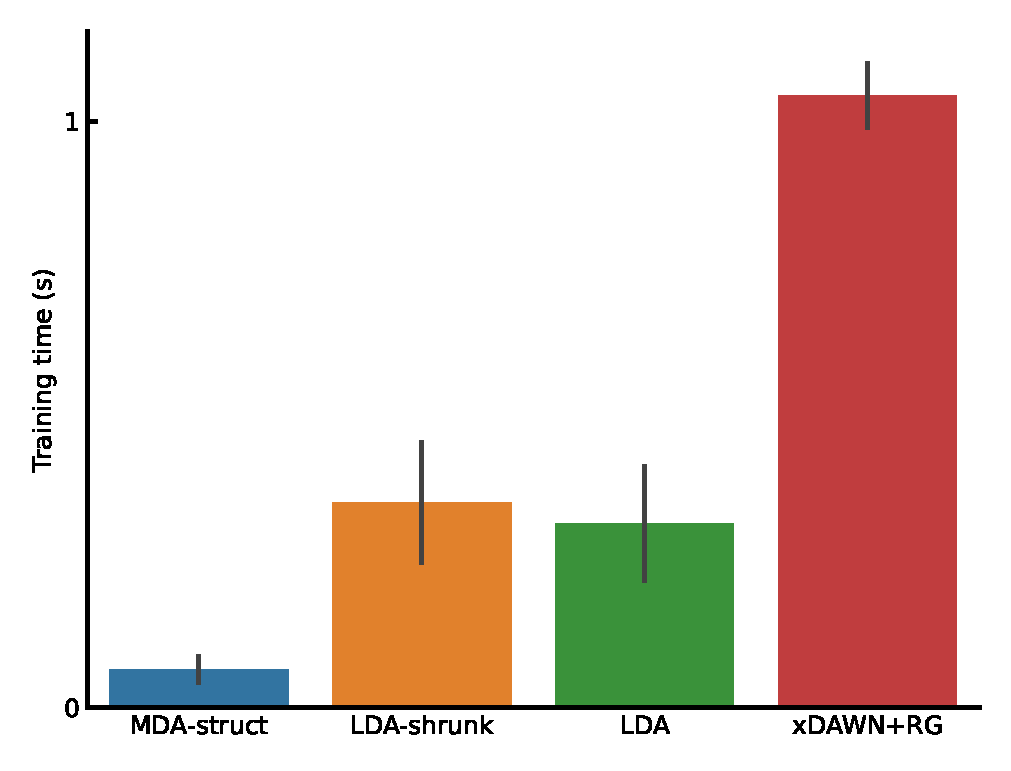
\includegraphics[width=.66\linewidth]{figures/stbf_struct/training_time.eps}
    \sffamily
    \hspace{-0.815469260193437in}
%% Creator: Matplotlib, PGF backend
%%
%% To include the figure in your LaTeX document, write
%%   \input{<filename>.pgf}
%%
%% Make sure the required packages are loaded in your preamble
%%   \usepackage{pgf}
%%
%% Also ensure that all the required font packages are loaded; for instance,
%% the lmodern package is sometimes necessary when using math font.
%%   \usepackage{lmodern}
%%
%% Figures using additional raster images can only be included by \input if
%% they are in the same directory as the main LaTeX file. For loading figures
%% from other directories you can use the `import` package
%%   \usepackage{import}
%%
%% and then include the figures with
%%   \import{<path to file>}{<filename>.pgf}
%%
%% Matplotlib used the following preamble
%%
\begingroup%
\makeatletter%
\begin{pgfpicture}%
\pgfpathrectangle{\pgfpointorigin}{\pgfqpoint{5.505894in}{1.391835in}}%
\pgfusepath{use as bounding box, clip}%
\begin{pgfscope}%
\pgfsetbuttcap%
\pgfsetmiterjoin%
\definecolor{currentfill}{rgb}{1.000000,1.000000,1.000000}%
\pgfsetfillcolor{currentfill}%
\pgfsetlinewidth{0.000000pt}%
\definecolor{currentstroke}{rgb}{1.000000,1.000000,1.000000}%
\pgfsetstrokecolor{currentstroke}%
\pgfsetdash{}{0pt}%
\pgfpathmoveto{\pgfqpoint{0.000000in}{0.000000in}}%
\pgfpathlineto{\pgfqpoint{5.505894in}{0.000000in}}%
\pgfpathlineto{\pgfqpoint{5.505894in}{1.391835in}}%
\pgfpathlineto{\pgfqpoint{0.000000in}{1.391835in}}%
\pgfpathlineto{\pgfqpoint{0.000000in}{0.000000in}}%
\pgfpathclose%
\pgfusepath{fill}%
\end{pgfscope}%
\begin{pgfscope}%
\pgfsetbuttcap%
\pgfsetmiterjoin%
\definecolor{currentfill}{rgb}{1.000000,1.000000,1.000000}%
\pgfsetfillcolor{currentfill}%
\pgfsetlinewidth{0.000000pt}%
\definecolor{currentstroke}{rgb}{0.000000,0.000000,0.000000}%
\pgfsetstrokecolor{currentstroke}%
\pgfsetstrokeopacity{0.000000}%
\pgfsetdash{}{0pt}%
\pgfpathmoveto{\pgfqpoint{0.776519in}{0.340278in}}%
\pgfpathlineto{\pgfqpoint{5.505894in}{0.340278in}}%
\pgfpathlineto{\pgfqpoint{5.505894in}{1.391835in}}%
\pgfpathlineto{\pgfqpoint{0.776519in}{1.391835in}}%
\pgfpathlineto{\pgfqpoint{0.776519in}{0.340278in}}%
\pgfpathclose%
\pgfusepath{fill}%
\end{pgfscope}%
\begin{pgfscope}%
\pgfpathrectangle{\pgfqpoint{0.776519in}{0.340278in}}{\pgfqpoint{4.729376in}{1.051557in}}%
\pgfusepath{clip}%
\pgfsetbuttcap%
\pgfsetroundjoin%
\definecolor{currentfill}{rgb}{0.949020,0.564706,0.094118}%
\pgfsetfillcolor{currentfill}%
\pgfsetlinewidth{0.000000pt}%
\definecolor{currentstroke}{rgb}{0.268235,0.268235,0.268235}%
\pgfsetstrokecolor{currentstroke}%
\pgfsetdash{}{0pt}%
\pgfpathmoveto{\pgfqpoint{1.074326in}{1.225427in}}%
\pgfpathcurveto{\pgfqpoint{1.078009in}{1.225427in}}{\pgfqpoint{1.081542in}{1.226891in}}{\pgfqpoint{1.084147in}{1.229495in}}%
\pgfpathcurveto{\pgfqpoint{1.086752in}{1.232100in}}{\pgfqpoint{1.088215in}{1.235633in}}{\pgfqpoint{1.088215in}{1.239316in}}%
\pgfpathcurveto{\pgfqpoint{1.088215in}{1.243000in}}{\pgfqpoint{1.086752in}{1.246533in}}{\pgfqpoint{1.084147in}{1.249137in}}%
\pgfpathcurveto{\pgfqpoint{1.081542in}{1.251742in}}{\pgfqpoint{1.078009in}{1.253205in}}{\pgfqpoint{1.074326in}{1.253205in}}%
\pgfpathcurveto{\pgfqpoint{1.070643in}{1.253205in}}{\pgfqpoint{1.067110in}{1.251742in}}{\pgfqpoint{1.064505in}{1.249137in}}%
\pgfpathcurveto{\pgfqpoint{1.061901in}{1.246533in}}{\pgfqpoint{1.060437in}{1.243000in}}{\pgfqpoint{1.060437in}{1.239316in}}%
\pgfpathcurveto{\pgfqpoint{1.060437in}{1.235633in}}{\pgfqpoint{1.061901in}{1.232100in}}{\pgfqpoint{1.064505in}{1.229495in}}%
\pgfpathcurveto{\pgfqpoint{1.067110in}{1.226891in}}{\pgfqpoint{1.070643in}{1.225427in}}{\pgfqpoint{1.074326in}{1.225427in}}%
\pgfpathlineto{\pgfqpoint{1.074326in}{1.225427in}}%
\pgfpathclose%
\pgfusepath{fill}%
\end{pgfscope}%
\begin{pgfscope}%
\pgfpathrectangle{\pgfqpoint{0.776519in}{0.340278in}}{\pgfqpoint{4.729376in}{1.051557in}}%
\pgfusepath{clip}%
\pgfsetbuttcap%
\pgfsetroundjoin%
\definecolor{currentfill}{rgb}{0.949020,0.564706,0.094118}%
\pgfsetfillcolor{currentfill}%
\pgfsetlinewidth{0.000000pt}%
\definecolor{currentstroke}{rgb}{0.268235,0.268235,0.268235}%
\pgfsetstrokecolor{currentstroke}%
\pgfsetdash{}{0pt}%
\pgfpathmoveto{\pgfqpoint{1.064702in}{1.230609in}}%
\pgfpathcurveto{\pgfqpoint{1.068385in}{1.230609in}}{\pgfqpoint{1.071918in}{1.232072in}}{\pgfqpoint{1.074523in}{1.234677in}}%
\pgfpathcurveto{\pgfqpoint{1.077127in}{1.237282in}}{\pgfqpoint{1.078591in}{1.240815in}}{\pgfqpoint{1.078591in}{1.244498in}}%
\pgfpathcurveto{\pgfqpoint{1.078591in}{1.248181in}}{\pgfqpoint{1.077127in}{1.251714in}}{\pgfqpoint{1.074523in}{1.254319in}}%
\pgfpathcurveto{\pgfqpoint{1.071918in}{1.256923in}}{\pgfqpoint{1.068385in}{1.258387in}}{\pgfqpoint{1.064702in}{1.258387in}}%
\pgfpathcurveto{\pgfqpoint{1.061018in}{1.258387in}}{\pgfqpoint{1.057485in}{1.256923in}}{\pgfqpoint{1.054881in}{1.254319in}}%
\pgfpathcurveto{\pgfqpoint{1.052276in}{1.251714in}}{\pgfqpoint{1.050813in}{1.248181in}}{\pgfqpoint{1.050813in}{1.244498in}}%
\pgfpathcurveto{\pgfqpoint{1.050813in}{1.240815in}}{\pgfqpoint{1.052276in}{1.237282in}}{\pgfqpoint{1.054881in}{1.234677in}}%
\pgfpathcurveto{\pgfqpoint{1.057485in}{1.232072in}}{\pgfqpoint{1.061018in}{1.230609in}}{\pgfqpoint{1.064702in}{1.230609in}}%
\pgfpathlineto{\pgfqpoint{1.064702in}{1.230609in}}%
\pgfpathclose%
\pgfusepath{fill}%
\end{pgfscope}%
\begin{pgfscope}%
\pgfpathrectangle{\pgfqpoint{0.776519in}{0.340278in}}{\pgfqpoint{4.729376in}{1.051557in}}%
\pgfusepath{clip}%
\pgfsetbuttcap%
\pgfsetroundjoin%
\definecolor{currentfill}{rgb}{0.949020,0.564706,0.094118}%
\pgfsetfillcolor{currentfill}%
\pgfsetlinewidth{0.000000pt}%
\definecolor{currentstroke}{rgb}{0.268235,0.268235,0.268235}%
\pgfsetstrokecolor{currentstroke}%
\pgfsetdash{}{0pt}%
\pgfpathmoveto{\pgfqpoint{1.129144in}{1.240384in}}%
\pgfpathcurveto{\pgfqpoint{1.132827in}{1.240384in}}{\pgfqpoint{1.136360in}{1.241847in}}{\pgfqpoint{1.138965in}{1.244452in}}%
\pgfpathcurveto{\pgfqpoint{1.141569in}{1.247056in}}{\pgfqpoint{1.143033in}{1.250589in}}{\pgfqpoint{1.143033in}{1.254272in}}%
\pgfpathcurveto{\pgfqpoint{1.143033in}{1.257956in}}{\pgfqpoint{1.141569in}{1.261489in}}{\pgfqpoint{1.138965in}{1.264093in}}%
\pgfpathcurveto{\pgfqpoint{1.136360in}{1.266698in}}{\pgfqpoint{1.132827in}{1.268161in}}{\pgfqpoint{1.129144in}{1.268161in}}%
\pgfpathcurveto{\pgfqpoint{1.125461in}{1.268161in}}{\pgfqpoint{1.121927in}{1.266698in}}{\pgfqpoint{1.119323in}{1.264093in}}%
\pgfpathcurveto{\pgfqpoint{1.116718in}{1.261489in}}{\pgfqpoint{1.115255in}{1.257956in}}{\pgfqpoint{1.115255in}{1.254272in}}%
\pgfpathcurveto{\pgfqpoint{1.115255in}{1.250589in}}{\pgfqpoint{1.116718in}{1.247056in}}{\pgfqpoint{1.119323in}{1.244452in}}%
\pgfpathcurveto{\pgfqpoint{1.121927in}{1.241847in}}{\pgfqpoint{1.125461in}{1.240384in}}{\pgfqpoint{1.129144in}{1.240384in}}%
\pgfpathlineto{\pgfqpoint{1.129144in}{1.240384in}}%
\pgfpathclose%
\pgfusepath{fill}%
\end{pgfscope}%
\begin{pgfscope}%
\pgfpathrectangle{\pgfqpoint{0.776519in}{0.340278in}}{\pgfqpoint{4.729376in}{1.051557in}}%
\pgfusepath{clip}%
\pgfsetbuttcap%
\pgfsetroundjoin%
\definecolor{currentfill}{rgb}{0.949020,0.564706,0.094118}%
\pgfsetfillcolor{currentfill}%
\pgfsetlinewidth{0.000000pt}%
\definecolor{currentstroke}{rgb}{0.268235,0.268235,0.268235}%
\pgfsetstrokecolor{currentstroke}%
\pgfsetdash{}{0pt}%
\pgfpathmoveto{\pgfqpoint{1.422570in}{1.263240in}}%
\pgfpathcurveto{\pgfqpoint{1.426254in}{1.263240in}}{\pgfqpoint{1.429787in}{1.264704in}}{\pgfqpoint{1.432391in}{1.267308in}}%
\pgfpathcurveto{\pgfqpoint{1.434996in}{1.269913in}}{\pgfqpoint{1.436459in}{1.273446in}}{\pgfqpoint{1.436459in}{1.277129in}}%
\pgfpathcurveto{\pgfqpoint{1.436459in}{1.280812in}}{\pgfqpoint{1.434996in}{1.284345in}}{\pgfqpoint{1.432391in}{1.286950in}}%
\pgfpathcurveto{\pgfqpoint{1.429787in}{1.289555in}}{\pgfqpoint{1.426254in}{1.291018in}}{\pgfqpoint{1.422570in}{1.291018in}}%
\pgfpathcurveto{\pgfqpoint{1.418887in}{1.291018in}}{\pgfqpoint{1.415354in}{1.289555in}}{\pgfqpoint{1.412749in}{1.286950in}}%
\pgfpathcurveto{\pgfqpoint{1.410145in}{1.284345in}}{\pgfqpoint{1.408681in}{1.280812in}}{\pgfqpoint{1.408681in}{1.277129in}}%
\pgfpathcurveto{\pgfqpoint{1.408681in}{1.273446in}}{\pgfqpoint{1.410145in}{1.269913in}}{\pgfqpoint{1.412749in}{1.267308in}}%
\pgfpathcurveto{\pgfqpoint{1.415354in}{1.264704in}}{\pgfqpoint{1.418887in}{1.263240in}}{\pgfqpoint{1.422570in}{1.263240in}}%
\pgfpathlineto{\pgfqpoint{1.422570in}{1.263240in}}%
\pgfpathclose%
\pgfusepath{fill}%
\end{pgfscope}%
\begin{pgfscope}%
\pgfpathrectangle{\pgfqpoint{0.776519in}{0.340278in}}{\pgfqpoint{4.729376in}{1.051557in}}%
\pgfusepath{clip}%
\pgfsetbuttcap%
\pgfsetroundjoin%
\definecolor{currentfill}{rgb}{0.949020,0.564706,0.094118}%
\pgfsetfillcolor{currentfill}%
\pgfsetlinewidth{0.000000pt}%
\definecolor{currentstroke}{rgb}{0.268235,0.268235,0.268235}%
\pgfsetstrokecolor{currentstroke}%
\pgfsetdash{}{0pt}%
\pgfpathmoveto{\pgfqpoint{1.034264in}{1.244351in}}%
\pgfpathcurveto{\pgfqpoint{1.037948in}{1.244351in}}{\pgfqpoint{1.041481in}{1.245814in}}{\pgfqpoint{1.044085in}{1.248419in}}%
\pgfpathcurveto{\pgfqpoint{1.046690in}{1.251023in}}{\pgfqpoint{1.048153in}{1.254556in}}{\pgfqpoint{1.048153in}{1.258239in}}%
\pgfpathcurveto{\pgfqpoint{1.048153in}{1.261923in}}{\pgfqpoint{1.046690in}{1.265456in}}{\pgfqpoint{1.044085in}{1.268060in}}%
\pgfpathcurveto{\pgfqpoint{1.041481in}{1.270665in}}{\pgfqpoint{1.037948in}{1.272128in}}{\pgfqpoint{1.034264in}{1.272128in}}%
\pgfpathcurveto{\pgfqpoint{1.030581in}{1.272128in}}{\pgfqpoint{1.027048in}{1.270665in}}{\pgfqpoint{1.024443in}{1.268060in}}%
\pgfpathcurveto{\pgfqpoint{1.021839in}{1.265456in}}{\pgfqpoint{1.020375in}{1.261923in}}{\pgfqpoint{1.020375in}{1.258239in}}%
\pgfpathcurveto{\pgfqpoint{1.020375in}{1.254556in}}{\pgfqpoint{1.021839in}{1.251023in}}{\pgfqpoint{1.024443in}{1.248419in}}%
\pgfpathcurveto{\pgfqpoint{1.027048in}{1.245814in}}{\pgfqpoint{1.030581in}{1.244351in}}{\pgfqpoint{1.034264in}{1.244351in}}%
\pgfpathlineto{\pgfqpoint{1.034264in}{1.244351in}}%
\pgfpathclose%
\pgfusepath{fill}%
\end{pgfscope}%
\begin{pgfscope}%
\pgfpathrectangle{\pgfqpoint{0.776519in}{0.340278in}}{\pgfqpoint{4.729376in}{1.051557in}}%
\pgfusepath{clip}%
\pgfsetbuttcap%
\pgfsetroundjoin%
\definecolor{currentfill}{rgb}{0.949020,0.564706,0.094118}%
\pgfsetfillcolor{currentfill}%
\pgfsetlinewidth{0.000000pt}%
\definecolor{currentstroke}{rgb}{0.268235,0.268235,0.268235}%
\pgfsetstrokecolor{currentstroke}%
\pgfsetdash{}{0pt}%
\pgfpathmoveto{\pgfqpoint{1.116293in}{1.242360in}}%
\pgfpathcurveto{\pgfqpoint{1.119976in}{1.242360in}}{\pgfqpoint{1.123509in}{1.243824in}}{\pgfqpoint{1.126113in}{1.246428in}}%
\pgfpathcurveto{\pgfqpoint{1.128718in}{1.249033in}}{\pgfqpoint{1.130181in}{1.252566in}}{\pgfqpoint{1.130181in}{1.256249in}}%
\pgfpathcurveto{\pgfqpoint{1.130181in}{1.259933in}}{\pgfqpoint{1.128718in}{1.263466in}}{\pgfqpoint{1.126113in}{1.266070in}}%
\pgfpathcurveto{\pgfqpoint{1.123509in}{1.268675in}}{\pgfqpoint{1.119976in}{1.270138in}}{\pgfqpoint{1.116293in}{1.270138in}}%
\pgfpathcurveto{\pgfqpoint{1.112609in}{1.270138in}}{\pgfqpoint{1.109076in}{1.268675in}}{\pgfqpoint{1.106472in}{1.266070in}}%
\pgfpathcurveto{\pgfqpoint{1.103867in}{1.263466in}}{\pgfqpoint{1.102404in}{1.259933in}}{\pgfqpoint{1.102404in}{1.256249in}}%
\pgfpathcurveto{\pgfqpoint{1.102404in}{1.252566in}}{\pgfqpoint{1.103867in}{1.249033in}}{\pgfqpoint{1.106472in}{1.246428in}}%
\pgfpathcurveto{\pgfqpoint{1.109076in}{1.243824in}}{\pgfqpoint{1.112609in}{1.242360in}}{\pgfqpoint{1.116293in}{1.242360in}}%
\pgfpathlineto{\pgfqpoint{1.116293in}{1.242360in}}%
\pgfpathclose%
\pgfusepath{fill}%
\end{pgfscope}%
\begin{pgfscope}%
\pgfpathrectangle{\pgfqpoint{0.776519in}{0.340278in}}{\pgfqpoint{4.729376in}{1.051557in}}%
\pgfusepath{clip}%
\pgfsetbuttcap%
\pgfsetroundjoin%
\definecolor{currentfill}{rgb}{0.949020,0.564706,0.094118}%
\pgfsetfillcolor{currentfill}%
\pgfsetlinewidth{0.000000pt}%
\definecolor{currentstroke}{rgb}{0.268235,0.268235,0.268235}%
\pgfsetstrokecolor{currentstroke}%
\pgfsetdash{}{0pt}%
\pgfpathmoveto{\pgfqpoint{1.120587in}{1.221468in}}%
\pgfpathcurveto{\pgfqpoint{1.124270in}{1.221468in}}{\pgfqpoint{1.127803in}{1.222931in}}{\pgfqpoint{1.130408in}{1.225536in}}%
\pgfpathcurveto{\pgfqpoint{1.133013in}{1.228140in}}{\pgfqpoint{1.134476in}{1.231673in}}{\pgfqpoint{1.134476in}{1.235356in}}%
\pgfpathcurveto{\pgfqpoint{1.134476in}{1.239040in}}{\pgfqpoint{1.133013in}{1.242573in}}{\pgfqpoint{1.130408in}{1.245177in}}%
\pgfpathcurveto{\pgfqpoint{1.127803in}{1.247782in}}{\pgfqpoint{1.124270in}{1.249245in}}{\pgfqpoint{1.120587in}{1.249245in}}%
\pgfpathcurveto{\pgfqpoint{1.116904in}{1.249245in}}{\pgfqpoint{1.113371in}{1.247782in}}{\pgfqpoint{1.110766in}{1.245177in}}%
\pgfpathcurveto{\pgfqpoint{1.108162in}{1.242573in}}{\pgfqpoint{1.106698in}{1.239040in}}{\pgfqpoint{1.106698in}{1.235356in}}%
\pgfpathcurveto{\pgfqpoint{1.106698in}{1.231673in}}{\pgfqpoint{1.108162in}{1.228140in}}{\pgfqpoint{1.110766in}{1.225536in}}%
\pgfpathcurveto{\pgfqpoint{1.113371in}{1.222931in}}{\pgfqpoint{1.116904in}{1.221468in}}{\pgfqpoint{1.120587in}{1.221468in}}%
\pgfpathlineto{\pgfqpoint{1.120587in}{1.221468in}}%
\pgfpathclose%
\pgfusepath{fill}%
\end{pgfscope}%
\begin{pgfscope}%
\pgfpathrectangle{\pgfqpoint{0.776519in}{0.340278in}}{\pgfqpoint{4.729376in}{1.051557in}}%
\pgfusepath{clip}%
\pgfsetbuttcap%
\pgfsetroundjoin%
\definecolor{currentfill}{rgb}{0.949020,0.564706,0.094118}%
\pgfsetfillcolor{currentfill}%
\pgfsetlinewidth{0.000000pt}%
\definecolor{currentstroke}{rgb}{0.268235,0.268235,0.268235}%
\pgfsetstrokecolor{currentstroke}%
\pgfsetdash{}{0pt}%
\pgfpathmoveto{\pgfqpoint{1.113086in}{1.237819in}}%
\pgfpathcurveto{\pgfqpoint{1.116770in}{1.237819in}}{\pgfqpoint{1.120303in}{1.239282in}}{\pgfqpoint{1.122907in}{1.241887in}}%
\pgfpathcurveto{\pgfqpoint{1.125512in}{1.244491in}}{\pgfqpoint{1.126975in}{1.248024in}}{\pgfqpoint{1.126975in}{1.251708in}}%
\pgfpathcurveto{\pgfqpoint{1.126975in}{1.255391in}}{\pgfqpoint{1.125512in}{1.258924in}}{\pgfqpoint{1.122907in}{1.261529in}}%
\pgfpathcurveto{\pgfqpoint{1.120303in}{1.264133in}}{\pgfqpoint{1.116770in}{1.265597in}}{\pgfqpoint{1.113086in}{1.265597in}}%
\pgfpathcurveto{\pgfqpoint{1.109403in}{1.265597in}}{\pgfqpoint{1.105870in}{1.264133in}}{\pgfqpoint{1.103265in}{1.261529in}}%
\pgfpathcurveto{\pgfqpoint{1.100661in}{1.258924in}}{\pgfqpoint{1.099197in}{1.255391in}}{\pgfqpoint{1.099197in}{1.251708in}}%
\pgfpathcurveto{\pgfqpoint{1.099197in}{1.248024in}}{\pgfqpoint{1.100661in}{1.244491in}}{\pgfqpoint{1.103265in}{1.241887in}}%
\pgfpathcurveto{\pgfqpoint{1.105870in}{1.239282in}}{\pgfqpoint{1.109403in}{1.237819in}}{\pgfqpoint{1.113086in}{1.237819in}}%
\pgfpathlineto{\pgfqpoint{1.113086in}{1.237819in}}%
\pgfpathclose%
\pgfusepath{fill}%
\end{pgfscope}%
\begin{pgfscope}%
\pgfpathrectangle{\pgfqpoint{0.776519in}{0.340278in}}{\pgfqpoint{4.729376in}{1.051557in}}%
\pgfusepath{clip}%
\pgfsetbuttcap%
\pgfsetroundjoin%
\definecolor{currentfill}{rgb}{0.949020,0.564706,0.094118}%
\pgfsetfillcolor{currentfill}%
\pgfsetlinewidth{0.000000pt}%
\definecolor{currentstroke}{rgb}{0.268235,0.268235,0.268235}%
\pgfsetstrokecolor{currentstroke}%
\pgfsetdash{}{0pt}%
\pgfpathmoveto{\pgfqpoint{1.005676in}{1.237285in}}%
\pgfpathcurveto{\pgfqpoint{1.009359in}{1.237285in}}{\pgfqpoint{1.012892in}{1.238749in}}{\pgfqpoint{1.015497in}{1.241353in}}%
\pgfpathcurveto{\pgfqpoint{1.018101in}{1.243958in}}{\pgfqpoint{1.019565in}{1.247491in}}{\pgfqpoint{1.019565in}{1.251174in}}%
\pgfpathcurveto{\pgfqpoint{1.019565in}{1.254857in}}{\pgfqpoint{1.018101in}{1.258390in}}{\pgfqpoint{1.015497in}{1.260995in}}%
\pgfpathcurveto{\pgfqpoint{1.012892in}{1.263600in}}{\pgfqpoint{1.009359in}{1.265063in}}{\pgfqpoint{1.005676in}{1.265063in}}%
\pgfpathcurveto{\pgfqpoint{1.001992in}{1.265063in}}{\pgfqpoint{0.998459in}{1.263600in}}{\pgfqpoint{0.995855in}{1.260995in}}%
\pgfpathcurveto{\pgfqpoint{0.993250in}{1.258390in}}{\pgfqpoint{0.991787in}{1.254857in}}{\pgfqpoint{0.991787in}{1.251174in}}%
\pgfpathcurveto{\pgfqpoint{0.991787in}{1.247491in}}{\pgfqpoint{0.993250in}{1.243958in}}{\pgfqpoint{0.995855in}{1.241353in}}%
\pgfpathcurveto{\pgfqpoint{0.998459in}{1.238749in}}{\pgfqpoint{1.001992in}{1.237285in}}{\pgfqpoint{1.005676in}{1.237285in}}%
\pgfpathlineto{\pgfqpoint{1.005676in}{1.237285in}}%
\pgfpathclose%
\pgfusepath{fill}%
\end{pgfscope}%
\begin{pgfscope}%
\pgfpathrectangle{\pgfqpoint{0.776519in}{0.340278in}}{\pgfqpoint{4.729376in}{1.051557in}}%
\pgfusepath{clip}%
\pgfsetbuttcap%
\pgfsetroundjoin%
\definecolor{currentfill}{rgb}{0.949020,0.564706,0.094118}%
\pgfsetfillcolor{currentfill}%
\pgfsetlinewidth{0.000000pt}%
\definecolor{currentstroke}{rgb}{0.268235,0.268235,0.268235}%
\pgfsetstrokecolor{currentstroke}%
\pgfsetdash{}{0pt}%
\pgfpathmoveto{\pgfqpoint{1.069484in}{1.237517in}}%
\pgfpathcurveto{\pgfqpoint{1.073168in}{1.237517in}}{\pgfqpoint{1.076701in}{1.238981in}}{\pgfqpoint{1.079305in}{1.241585in}}%
\pgfpathcurveto{\pgfqpoint{1.081910in}{1.244190in}}{\pgfqpoint{1.083373in}{1.247723in}}{\pgfqpoint{1.083373in}{1.251406in}}%
\pgfpathcurveto{\pgfqpoint{1.083373in}{1.255090in}}{\pgfqpoint{1.081910in}{1.258623in}}{\pgfqpoint{1.079305in}{1.261227in}}%
\pgfpathcurveto{\pgfqpoint{1.076701in}{1.263832in}}{\pgfqpoint{1.073168in}{1.265295in}}{\pgfqpoint{1.069484in}{1.265295in}}%
\pgfpathcurveto{\pgfqpoint{1.065801in}{1.265295in}}{\pgfqpoint{1.062268in}{1.263832in}}{\pgfqpoint{1.059663in}{1.261227in}}%
\pgfpathcurveto{\pgfqpoint{1.057059in}{1.258623in}}{\pgfqpoint{1.055595in}{1.255090in}}{\pgfqpoint{1.055595in}{1.251406in}}%
\pgfpathcurveto{\pgfqpoint{1.055595in}{1.247723in}}{\pgfqpoint{1.057059in}{1.244190in}}{\pgfqpoint{1.059663in}{1.241585in}}%
\pgfpathcurveto{\pgfqpoint{1.062268in}{1.238981in}}{\pgfqpoint{1.065801in}{1.237517in}}{\pgfqpoint{1.069484in}{1.237517in}}%
\pgfpathlineto{\pgfqpoint{1.069484in}{1.237517in}}%
\pgfpathclose%
\pgfusepath{fill}%
\end{pgfscope}%
\begin{pgfscope}%
\pgfpathrectangle{\pgfqpoint{0.776519in}{0.340278in}}{\pgfqpoint{4.729376in}{1.051557in}}%
\pgfusepath{clip}%
\pgfsetbuttcap%
\pgfsetroundjoin%
\definecolor{currentfill}{rgb}{0.949020,0.564706,0.094118}%
\pgfsetfillcolor{currentfill}%
\pgfsetlinewidth{0.000000pt}%
\definecolor{currentstroke}{rgb}{0.268235,0.268235,0.268235}%
\pgfsetstrokecolor{currentstroke}%
\pgfsetdash{}{0pt}%
\pgfpathmoveto{\pgfqpoint{1.082397in}{1.230423in}}%
\pgfpathcurveto{\pgfqpoint{1.086081in}{1.230423in}}{\pgfqpoint{1.089614in}{1.231886in}}{\pgfqpoint{1.092218in}{1.234491in}}%
\pgfpathcurveto{\pgfqpoint{1.094823in}{1.237095in}}{\pgfqpoint{1.096286in}{1.240628in}}{\pgfqpoint{1.096286in}{1.244311in}}%
\pgfpathcurveto{\pgfqpoint{1.096286in}{1.247995in}}{\pgfqpoint{1.094823in}{1.251528in}}{\pgfqpoint{1.092218in}{1.254132in}}%
\pgfpathcurveto{\pgfqpoint{1.089614in}{1.256737in}}{\pgfqpoint{1.086081in}{1.258200in}}{\pgfqpoint{1.082397in}{1.258200in}}%
\pgfpathcurveto{\pgfqpoint{1.078714in}{1.258200in}}{\pgfqpoint{1.075181in}{1.256737in}}{\pgfqpoint{1.072577in}{1.254132in}}%
\pgfpathcurveto{\pgfqpoint{1.069972in}{1.251528in}}{\pgfqpoint{1.068509in}{1.247995in}}{\pgfqpoint{1.068509in}{1.244311in}}%
\pgfpathcurveto{\pgfqpoint{1.068509in}{1.240628in}}{\pgfqpoint{1.069972in}{1.237095in}}{\pgfqpoint{1.072577in}{1.234491in}}%
\pgfpathcurveto{\pgfqpoint{1.075181in}{1.231886in}}{\pgfqpoint{1.078714in}{1.230423in}}{\pgfqpoint{1.082397in}{1.230423in}}%
\pgfpathlineto{\pgfqpoint{1.082397in}{1.230423in}}%
\pgfpathclose%
\pgfusepath{fill}%
\end{pgfscope}%
\begin{pgfscope}%
\pgfpathrectangle{\pgfqpoint{0.776519in}{0.340278in}}{\pgfqpoint{4.729376in}{1.051557in}}%
\pgfusepath{clip}%
\pgfsetbuttcap%
\pgfsetroundjoin%
\definecolor{currentfill}{rgb}{0.949020,0.564706,0.094118}%
\pgfsetfillcolor{currentfill}%
\pgfsetlinewidth{0.000000pt}%
\definecolor{currentstroke}{rgb}{0.268235,0.268235,0.268235}%
\pgfsetstrokecolor{currentstroke}%
\pgfsetdash{}{0pt}%
\pgfpathmoveto{\pgfqpoint{1.430721in}{1.231903in}}%
\pgfpathcurveto{\pgfqpoint{1.434405in}{1.231903in}}{\pgfqpoint{1.437938in}{1.233366in}}{\pgfqpoint{1.440542in}{1.235971in}}%
\pgfpathcurveto{\pgfqpoint{1.443147in}{1.238575in}}{\pgfqpoint{1.444610in}{1.242108in}}{\pgfqpoint{1.444610in}{1.245792in}}%
\pgfpathcurveto{\pgfqpoint{1.444610in}{1.249475in}}{\pgfqpoint{1.443147in}{1.253008in}}{\pgfqpoint{1.440542in}{1.255612in}}%
\pgfpathcurveto{\pgfqpoint{1.437938in}{1.258217in}}{\pgfqpoint{1.434405in}{1.259680in}}{\pgfqpoint{1.430721in}{1.259680in}}%
\pgfpathcurveto{\pgfqpoint{1.427038in}{1.259680in}}{\pgfqpoint{1.423505in}{1.258217in}}{\pgfqpoint{1.420901in}{1.255612in}}%
\pgfpathcurveto{\pgfqpoint{1.418296in}{1.253008in}}{\pgfqpoint{1.416833in}{1.249475in}}{\pgfqpoint{1.416833in}{1.245792in}}%
\pgfpathcurveto{\pgfqpoint{1.416833in}{1.242108in}}{\pgfqpoint{1.418296in}{1.238575in}}{\pgfqpoint{1.420901in}{1.235971in}}%
\pgfpathcurveto{\pgfqpoint{1.423505in}{1.233366in}}{\pgfqpoint{1.427038in}{1.231903in}}{\pgfqpoint{1.430721in}{1.231903in}}%
\pgfpathlineto{\pgfqpoint{1.430721in}{1.231903in}}%
\pgfpathclose%
\pgfusepath{fill}%
\end{pgfscope}%
\begin{pgfscope}%
\pgfpathrectangle{\pgfqpoint{0.776519in}{0.340278in}}{\pgfqpoint{4.729376in}{1.051557in}}%
\pgfusepath{clip}%
\pgfsetbuttcap%
\pgfsetroundjoin%
\definecolor{currentfill}{rgb}{0.949020,0.564706,0.094118}%
\pgfsetfillcolor{currentfill}%
\pgfsetlinewidth{0.000000pt}%
\definecolor{currentstroke}{rgb}{0.268235,0.268235,0.268235}%
\pgfsetstrokecolor{currentstroke}%
\pgfsetdash{}{0pt}%
\pgfpathmoveto{\pgfqpoint{1.040704in}{1.269728in}}%
\pgfpathcurveto{\pgfqpoint{1.044387in}{1.269728in}}{\pgfqpoint{1.047920in}{1.271191in}}{\pgfqpoint{1.050525in}{1.273796in}}%
\pgfpathcurveto{\pgfqpoint{1.053129in}{1.276400in}}{\pgfqpoint{1.054593in}{1.279933in}}{\pgfqpoint{1.054593in}{1.283617in}}%
\pgfpathcurveto{\pgfqpoint{1.054593in}{1.287300in}}{\pgfqpoint{1.053129in}{1.290833in}}{\pgfqpoint{1.050525in}{1.293438in}}%
\pgfpathcurveto{\pgfqpoint{1.047920in}{1.296042in}}{\pgfqpoint{1.044387in}{1.297506in}}{\pgfqpoint{1.040704in}{1.297506in}}%
\pgfpathcurveto{\pgfqpoint{1.037021in}{1.297506in}}{\pgfqpoint{1.033488in}{1.296042in}}{\pgfqpoint{1.030883in}{1.293438in}}%
\pgfpathcurveto{\pgfqpoint{1.028279in}{1.290833in}}{\pgfqpoint{1.026815in}{1.287300in}}{\pgfqpoint{1.026815in}{1.283617in}}%
\pgfpathcurveto{\pgfqpoint{1.026815in}{1.279933in}}{\pgfqpoint{1.028279in}{1.276400in}}{\pgfqpoint{1.030883in}{1.273796in}}%
\pgfpathcurveto{\pgfqpoint{1.033488in}{1.271191in}}{\pgfqpoint{1.037021in}{1.269728in}}{\pgfqpoint{1.040704in}{1.269728in}}%
\pgfpathlineto{\pgfqpoint{1.040704in}{1.269728in}}%
\pgfpathclose%
\pgfusepath{fill}%
\end{pgfscope}%
\begin{pgfscope}%
\pgfpathrectangle{\pgfqpoint{0.776519in}{0.340278in}}{\pgfqpoint{4.729376in}{1.051557in}}%
\pgfusepath{clip}%
\pgfsetbuttcap%
\pgfsetroundjoin%
\definecolor{currentfill}{rgb}{0.949020,0.564706,0.094118}%
\pgfsetfillcolor{currentfill}%
\pgfsetlinewidth{0.000000pt}%
\definecolor{currentstroke}{rgb}{0.268235,0.268235,0.268235}%
\pgfsetstrokecolor{currentstroke}%
\pgfsetdash{}{0pt}%
\pgfpathmoveto{\pgfqpoint{1.418670in}{1.257981in}}%
\pgfpathcurveto{\pgfqpoint{1.422353in}{1.257981in}}{\pgfqpoint{1.425886in}{1.259444in}}{\pgfqpoint{1.428491in}{1.262049in}}%
\pgfpathcurveto{\pgfqpoint{1.431095in}{1.264653in}}{\pgfqpoint{1.432559in}{1.268186in}}{\pgfqpoint{1.432559in}{1.271870in}}%
\pgfpathcurveto{\pgfqpoint{1.432559in}{1.275553in}}{\pgfqpoint{1.431095in}{1.279086in}}{\pgfqpoint{1.428491in}{1.281691in}}%
\pgfpathcurveto{\pgfqpoint{1.425886in}{1.284295in}}{\pgfqpoint{1.422353in}{1.285759in}}{\pgfqpoint{1.418670in}{1.285759in}}%
\pgfpathcurveto{\pgfqpoint{1.414986in}{1.285759in}}{\pgfqpoint{1.411453in}{1.284295in}}{\pgfqpoint{1.408849in}{1.281691in}}%
\pgfpathcurveto{\pgfqpoint{1.406244in}{1.279086in}}{\pgfqpoint{1.404781in}{1.275553in}}{\pgfqpoint{1.404781in}{1.271870in}}%
\pgfpathcurveto{\pgfqpoint{1.404781in}{1.268186in}}{\pgfqpoint{1.406244in}{1.264653in}}{\pgfqpoint{1.408849in}{1.262049in}}%
\pgfpathcurveto{\pgfqpoint{1.411453in}{1.259444in}}{\pgfqpoint{1.414986in}{1.257981in}}{\pgfqpoint{1.418670in}{1.257981in}}%
\pgfpathlineto{\pgfqpoint{1.418670in}{1.257981in}}%
\pgfpathclose%
\pgfusepath{fill}%
\end{pgfscope}%
\begin{pgfscope}%
\pgfpathrectangle{\pgfqpoint{0.776519in}{0.340278in}}{\pgfqpoint{4.729376in}{1.051557in}}%
\pgfusepath{clip}%
\pgfsetbuttcap%
\pgfsetroundjoin%
\definecolor{currentfill}{rgb}{0.949020,0.564706,0.094118}%
\pgfsetfillcolor{currentfill}%
\pgfsetlinewidth{0.000000pt}%
\definecolor{currentstroke}{rgb}{0.268235,0.268235,0.268235}%
\pgfsetstrokecolor{currentstroke}%
\pgfsetdash{}{0pt}%
\pgfpathmoveto{\pgfqpoint{1.076331in}{1.224250in}}%
\pgfpathcurveto{\pgfqpoint{1.080014in}{1.224250in}}{\pgfqpoint{1.083547in}{1.225713in}}{\pgfqpoint{1.086152in}{1.228318in}}%
\pgfpathcurveto{\pgfqpoint{1.088757in}{1.230922in}}{\pgfqpoint{1.090220in}{1.234455in}}{\pgfqpoint{1.090220in}{1.238139in}}%
\pgfpathcurveto{\pgfqpoint{1.090220in}{1.241822in}}{\pgfqpoint{1.088757in}{1.245355in}}{\pgfqpoint{1.086152in}{1.247960in}}%
\pgfpathcurveto{\pgfqpoint{1.083547in}{1.250564in}}{\pgfqpoint{1.080014in}{1.252028in}}{\pgfqpoint{1.076331in}{1.252028in}}%
\pgfpathcurveto{\pgfqpoint{1.072648in}{1.252028in}}{\pgfqpoint{1.069115in}{1.250564in}}{\pgfqpoint{1.066510in}{1.247960in}}%
\pgfpathcurveto{\pgfqpoint{1.063906in}{1.245355in}}{\pgfqpoint{1.062442in}{1.241822in}}{\pgfqpoint{1.062442in}{1.238139in}}%
\pgfpathcurveto{\pgfqpoint{1.062442in}{1.234455in}}{\pgfqpoint{1.063906in}{1.230922in}}{\pgfqpoint{1.066510in}{1.228318in}}%
\pgfpathcurveto{\pgfqpoint{1.069115in}{1.225713in}}{\pgfqpoint{1.072648in}{1.224250in}}{\pgfqpoint{1.076331in}{1.224250in}}%
\pgfpathlineto{\pgfqpoint{1.076331in}{1.224250in}}%
\pgfpathclose%
\pgfusepath{fill}%
\end{pgfscope}%
\begin{pgfscope}%
\pgfpathrectangle{\pgfqpoint{0.776519in}{0.340278in}}{\pgfqpoint{4.729376in}{1.051557in}}%
\pgfusepath{clip}%
\pgfsetbuttcap%
\pgfsetroundjoin%
\definecolor{currentfill}{rgb}{0.949020,0.564706,0.094118}%
\pgfsetfillcolor{currentfill}%
\pgfsetlinewidth{0.000000pt}%
\definecolor{currentstroke}{rgb}{0.268235,0.268235,0.268235}%
\pgfsetstrokecolor{currentstroke}%
\pgfsetdash{}{0pt}%
\pgfpathmoveto{\pgfqpoint{1.427116in}{1.224118in}}%
\pgfpathcurveto{\pgfqpoint{1.430799in}{1.224118in}}{\pgfqpoint{1.434332in}{1.225582in}}{\pgfqpoint{1.436937in}{1.228186in}}%
\pgfpathcurveto{\pgfqpoint{1.439541in}{1.230791in}}{\pgfqpoint{1.441005in}{1.234324in}}{\pgfqpoint{1.441005in}{1.238007in}}%
\pgfpathcurveto{\pgfqpoint{1.441005in}{1.241691in}}{\pgfqpoint{1.439541in}{1.245224in}}{\pgfqpoint{1.436937in}{1.247828in}}%
\pgfpathcurveto{\pgfqpoint{1.434332in}{1.250433in}}{\pgfqpoint{1.430799in}{1.251896in}}{\pgfqpoint{1.427116in}{1.251896in}}%
\pgfpathcurveto{\pgfqpoint{1.423432in}{1.251896in}}{\pgfqpoint{1.419899in}{1.250433in}}{\pgfqpoint{1.417295in}{1.247828in}}%
\pgfpathcurveto{\pgfqpoint{1.414690in}{1.245224in}}{\pgfqpoint{1.413227in}{1.241691in}}{\pgfqpoint{1.413227in}{1.238007in}}%
\pgfpathcurveto{\pgfqpoint{1.413227in}{1.234324in}}{\pgfqpoint{1.414690in}{1.230791in}}{\pgfqpoint{1.417295in}{1.228186in}}%
\pgfpathcurveto{\pgfqpoint{1.419899in}{1.225582in}}{\pgfqpoint{1.423432in}{1.224118in}}{\pgfqpoint{1.427116in}{1.224118in}}%
\pgfpathlineto{\pgfqpoint{1.427116in}{1.224118in}}%
\pgfpathclose%
\pgfusepath{fill}%
\end{pgfscope}%
\begin{pgfscope}%
\pgfpathrectangle{\pgfqpoint{0.776519in}{0.340278in}}{\pgfqpoint{4.729376in}{1.051557in}}%
\pgfusepath{clip}%
\pgfsetbuttcap%
\pgfsetroundjoin%
\definecolor{currentfill}{rgb}{0.949020,0.564706,0.094118}%
\pgfsetfillcolor{currentfill}%
\pgfsetlinewidth{0.000000pt}%
\definecolor{currentstroke}{rgb}{0.268235,0.268235,0.268235}%
\pgfsetstrokecolor{currentstroke}%
\pgfsetdash{}{0pt}%
\pgfpathmoveto{\pgfqpoint{1.044146in}{1.271035in}}%
\pgfpathcurveto{\pgfqpoint{1.047829in}{1.271035in}}{\pgfqpoint{1.051362in}{1.272498in}}{\pgfqpoint{1.053967in}{1.275103in}}%
\pgfpathcurveto{\pgfqpoint{1.056572in}{1.277707in}}{\pgfqpoint{1.058035in}{1.281240in}}{\pgfqpoint{1.058035in}{1.284923in}}%
\pgfpathcurveto{\pgfqpoint{1.058035in}{1.288607in}}{\pgfqpoint{1.056572in}{1.292140in}}{\pgfqpoint{1.053967in}{1.294744in}}%
\pgfpathcurveto{\pgfqpoint{1.051362in}{1.297349in}}{\pgfqpoint{1.047829in}{1.298812in}}{\pgfqpoint{1.044146in}{1.298812in}}%
\pgfpathcurveto{\pgfqpoint{1.040463in}{1.298812in}}{\pgfqpoint{1.036930in}{1.297349in}}{\pgfqpoint{1.034325in}{1.294744in}}%
\pgfpathcurveto{\pgfqpoint{1.031721in}{1.292140in}}{\pgfqpoint{1.030257in}{1.288607in}}{\pgfqpoint{1.030257in}{1.284923in}}%
\pgfpathcurveto{\pgfqpoint{1.030257in}{1.281240in}}{\pgfqpoint{1.031721in}{1.277707in}}{\pgfqpoint{1.034325in}{1.275103in}}%
\pgfpathcurveto{\pgfqpoint{1.036930in}{1.272498in}}{\pgfqpoint{1.040463in}{1.271035in}}{\pgfqpoint{1.044146in}{1.271035in}}%
\pgfpathlineto{\pgfqpoint{1.044146in}{1.271035in}}%
\pgfpathclose%
\pgfusepath{fill}%
\end{pgfscope}%
\begin{pgfscope}%
\pgfpathrectangle{\pgfqpoint{0.776519in}{0.340278in}}{\pgfqpoint{4.729376in}{1.051557in}}%
\pgfusepath{clip}%
\pgfsetbuttcap%
\pgfsetroundjoin%
\definecolor{currentfill}{rgb}{0.949020,0.564706,0.094118}%
\pgfsetfillcolor{currentfill}%
\pgfsetlinewidth{0.000000pt}%
\definecolor{currentstroke}{rgb}{0.268235,0.268235,0.268235}%
\pgfsetstrokecolor{currentstroke}%
\pgfsetdash{}{0pt}%
\pgfpathmoveto{\pgfqpoint{1.105339in}{1.249785in}}%
\pgfpathcurveto{\pgfqpoint{1.109023in}{1.249785in}}{\pgfqpoint{1.112556in}{1.251249in}}{\pgfqpoint{1.115160in}{1.253853in}}%
\pgfpathcurveto{\pgfqpoint{1.117765in}{1.256458in}}{\pgfqpoint{1.119228in}{1.259991in}}{\pgfqpoint{1.119228in}{1.263674in}}%
\pgfpathcurveto{\pgfqpoint{1.119228in}{1.267358in}}{\pgfqpoint{1.117765in}{1.270891in}}{\pgfqpoint{1.115160in}{1.273495in}}%
\pgfpathcurveto{\pgfqpoint{1.112556in}{1.276100in}}{\pgfqpoint{1.109023in}{1.277563in}}{\pgfqpoint{1.105339in}{1.277563in}}%
\pgfpathcurveto{\pgfqpoint{1.101656in}{1.277563in}}{\pgfqpoint{1.098123in}{1.276100in}}{\pgfqpoint{1.095518in}{1.273495in}}%
\pgfpathcurveto{\pgfqpoint{1.092914in}{1.270891in}}{\pgfqpoint{1.091450in}{1.267358in}}{\pgfqpoint{1.091450in}{1.263674in}}%
\pgfpathcurveto{\pgfqpoint{1.091450in}{1.259991in}}{\pgfqpoint{1.092914in}{1.256458in}}{\pgfqpoint{1.095518in}{1.253853in}}%
\pgfpathcurveto{\pgfqpoint{1.098123in}{1.251249in}}{\pgfqpoint{1.101656in}{1.249785in}}{\pgfqpoint{1.105339in}{1.249785in}}%
\pgfpathlineto{\pgfqpoint{1.105339in}{1.249785in}}%
\pgfpathclose%
\pgfusepath{fill}%
\end{pgfscope}%
\begin{pgfscope}%
\pgfpathrectangle{\pgfqpoint{0.776519in}{0.340278in}}{\pgfqpoint{4.729376in}{1.051557in}}%
\pgfusepath{clip}%
\pgfsetbuttcap%
\pgfsetroundjoin%
\definecolor{currentfill}{rgb}{0.949020,0.564706,0.094118}%
\pgfsetfillcolor{currentfill}%
\pgfsetlinewidth{0.000000pt}%
\definecolor{currentstroke}{rgb}{0.268235,0.268235,0.268235}%
\pgfsetstrokecolor{currentstroke}%
\pgfsetdash{}{0pt}%
\pgfpathmoveto{\pgfqpoint{1.118113in}{1.220818in}}%
\pgfpathcurveto{\pgfqpoint{1.121797in}{1.220818in}}{\pgfqpoint{1.125330in}{1.222282in}}{\pgfqpoint{1.127934in}{1.224886in}}%
\pgfpathcurveto{\pgfqpoint{1.130539in}{1.227491in}}{\pgfqpoint{1.132002in}{1.231024in}}{\pgfqpoint{1.132002in}{1.234707in}}%
\pgfpathcurveto{\pgfqpoint{1.132002in}{1.238391in}}{\pgfqpoint{1.130539in}{1.241924in}}{\pgfqpoint{1.127934in}{1.244528in}}%
\pgfpathcurveto{\pgfqpoint{1.125330in}{1.247133in}}{\pgfqpoint{1.121797in}{1.248596in}}{\pgfqpoint{1.118113in}{1.248596in}}%
\pgfpathcurveto{\pgfqpoint{1.114430in}{1.248596in}}{\pgfqpoint{1.110897in}{1.247133in}}{\pgfqpoint{1.108292in}{1.244528in}}%
\pgfpathcurveto{\pgfqpoint{1.105688in}{1.241924in}}{\pgfqpoint{1.104224in}{1.238391in}}{\pgfqpoint{1.104224in}{1.234707in}}%
\pgfpathcurveto{\pgfqpoint{1.104224in}{1.231024in}}{\pgfqpoint{1.105688in}{1.227491in}}{\pgfqpoint{1.108292in}{1.224886in}}%
\pgfpathcurveto{\pgfqpoint{1.110897in}{1.222282in}}{\pgfqpoint{1.114430in}{1.220818in}}{\pgfqpoint{1.118113in}{1.220818in}}%
\pgfpathlineto{\pgfqpoint{1.118113in}{1.220818in}}%
\pgfpathclose%
\pgfusepath{fill}%
\end{pgfscope}%
\begin{pgfscope}%
\pgfpathrectangle{\pgfqpoint{0.776519in}{0.340278in}}{\pgfqpoint{4.729376in}{1.051557in}}%
\pgfusepath{clip}%
\pgfsetbuttcap%
\pgfsetroundjoin%
\definecolor{currentfill}{rgb}{0.949020,0.564706,0.094118}%
\pgfsetfillcolor{currentfill}%
\pgfsetlinewidth{0.000000pt}%
\definecolor{currentstroke}{rgb}{0.268235,0.268235,0.268235}%
\pgfsetstrokecolor{currentstroke}%
\pgfsetdash{}{0pt}%
\pgfpathmoveto{\pgfqpoint{1.136390in}{1.227008in}}%
\pgfpathcurveto{\pgfqpoint{1.140073in}{1.227008in}}{\pgfqpoint{1.143606in}{1.228471in}}{\pgfqpoint{1.146211in}{1.231076in}}%
\pgfpathcurveto{\pgfqpoint{1.148815in}{1.233680in}}{\pgfqpoint{1.150279in}{1.237213in}}{\pgfqpoint{1.150279in}{1.240897in}}%
\pgfpathcurveto{\pgfqpoint{1.150279in}{1.244580in}}{\pgfqpoint{1.148815in}{1.248113in}}{\pgfqpoint{1.146211in}{1.250717in}}%
\pgfpathcurveto{\pgfqpoint{1.143606in}{1.253322in}}{\pgfqpoint{1.140073in}{1.254785in}}{\pgfqpoint{1.136390in}{1.254785in}}%
\pgfpathcurveto{\pgfqpoint{1.132706in}{1.254785in}}{\pgfqpoint{1.129173in}{1.253322in}}{\pgfqpoint{1.126569in}{1.250717in}}%
\pgfpathcurveto{\pgfqpoint{1.123964in}{1.248113in}}{\pgfqpoint{1.122501in}{1.244580in}}{\pgfqpoint{1.122501in}{1.240897in}}%
\pgfpathcurveto{\pgfqpoint{1.122501in}{1.237213in}}{\pgfqpoint{1.123964in}{1.233680in}}{\pgfqpoint{1.126569in}{1.231076in}}%
\pgfpathcurveto{\pgfqpoint{1.129173in}{1.228471in}}{\pgfqpoint{1.132706in}{1.227008in}}{\pgfqpoint{1.136390in}{1.227008in}}%
\pgfpathlineto{\pgfqpoint{1.136390in}{1.227008in}}%
\pgfpathclose%
\pgfusepath{fill}%
\end{pgfscope}%
\begin{pgfscope}%
\pgfpathrectangle{\pgfqpoint{0.776519in}{0.340278in}}{\pgfqpoint{4.729376in}{1.051557in}}%
\pgfusepath{clip}%
\pgfsetbuttcap%
\pgfsetroundjoin%
\definecolor{currentfill}{rgb}{0.949020,0.564706,0.094118}%
\pgfsetfillcolor{currentfill}%
\pgfsetlinewidth{0.000000pt}%
\definecolor{currentstroke}{rgb}{0.268235,0.268235,0.268235}%
\pgfsetstrokecolor{currentstroke}%
\pgfsetdash{}{0pt}%
\pgfpathmoveto{\pgfqpoint{0.994046in}{1.226690in}}%
\pgfpathcurveto{\pgfqpoint{0.997730in}{1.226690in}}{\pgfqpoint{1.001263in}{1.228153in}}{\pgfqpoint{1.003867in}{1.230758in}}%
\pgfpathcurveto{\pgfqpoint{1.006472in}{1.233362in}}{\pgfqpoint{1.007935in}{1.236895in}}{\pgfqpoint{1.007935in}{1.240579in}}%
\pgfpathcurveto{\pgfqpoint{1.007935in}{1.244262in}}{\pgfqpoint{1.006472in}{1.247795in}}{\pgfqpoint{1.003867in}{1.250400in}}%
\pgfpathcurveto{\pgfqpoint{1.001263in}{1.253004in}}{\pgfqpoint{0.997730in}{1.254468in}}{\pgfqpoint{0.994046in}{1.254468in}}%
\pgfpathcurveto{\pgfqpoint{0.990363in}{1.254468in}}{\pgfqpoint{0.986830in}{1.253004in}}{\pgfqpoint{0.984226in}{1.250400in}}%
\pgfpathcurveto{\pgfqpoint{0.981621in}{1.247795in}}{\pgfqpoint{0.980158in}{1.244262in}}{\pgfqpoint{0.980158in}{1.240579in}}%
\pgfpathcurveto{\pgfqpoint{0.980158in}{1.236895in}}{\pgfqpoint{0.981621in}{1.233362in}}{\pgfqpoint{0.984226in}{1.230758in}}%
\pgfpathcurveto{\pgfqpoint{0.986830in}{1.228153in}}{\pgfqpoint{0.990363in}{1.226690in}}{\pgfqpoint{0.994046in}{1.226690in}}%
\pgfpathlineto{\pgfqpoint{0.994046in}{1.226690in}}%
\pgfpathclose%
\pgfusepath{fill}%
\end{pgfscope}%
\begin{pgfscope}%
\pgfpathrectangle{\pgfqpoint{0.776519in}{0.340278in}}{\pgfqpoint{4.729376in}{1.051557in}}%
\pgfusepath{clip}%
\pgfsetbuttcap%
\pgfsetroundjoin%
\definecolor{currentfill}{rgb}{0.949020,0.564706,0.094118}%
\pgfsetfillcolor{currentfill}%
\pgfsetlinewidth{0.000000pt}%
\definecolor{currentstroke}{rgb}{0.268235,0.268235,0.268235}%
\pgfsetstrokecolor{currentstroke}%
\pgfsetdash{}{0pt}%
\pgfpathmoveto{\pgfqpoint{1.126487in}{1.244598in}}%
\pgfpathcurveto{\pgfqpoint{1.130171in}{1.244598in}}{\pgfqpoint{1.133704in}{1.246062in}}{\pgfqpoint{1.136308in}{1.248666in}}%
\pgfpathcurveto{\pgfqpoint{1.138913in}{1.251271in}}{\pgfqpoint{1.140376in}{1.254804in}}{\pgfqpoint{1.140376in}{1.258487in}}%
\pgfpathcurveto{\pgfqpoint{1.140376in}{1.262171in}}{\pgfqpoint{1.138913in}{1.265704in}}{\pgfqpoint{1.136308in}{1.268308in}}%
\pgfpathcurveto{\pgfqpoint{1.133704in}{1.270913in}}{\pgfqpoint{1.130171in}{1.272376in}}{\pgfqpoint{1.126487in}{1.272376in}}%
\pgfpathcurveto{\pgfqpoint{1.122804in}{1.272376in}}{\pgfqpoint{1.119271in}{1.270913in}}{\pgfqpoint{1.116666in}{1.268308in}}%
\pgfpathcurveto{\pgfqpoint{1.114062in}{1.265704in}}{\pgfqpoint{1.112598in}{1.262171in}}{\pgfqpoint{1.112598in}{1.258487in}}%
\pgfpathcurveto{\pgfqpoint{1.112598in}{1.254804in}}{\pgfqpoint{1.114062in}{1.251271in}}{\pgfqpoint{1.116666in}{1.248666in}}%
\pgfpathcurveto{\pgfqpoint{1.119271in}{1.246062in}}{\pgfqpoint{1.122804in}{1.244598in}}{\pgfqpoint{1.126487in}{1.244598in}}%
\pgfpathlineto{\pgfqpoint{1.126487in}{1.244598in}}%
\pgfpathclose%
\pgfusepath{fill}%
\end{pgfscope}%
\begin{pgfscope}%
\pgfpathrectangle{\pgfqpoint{0.776519in}{0.340278in}}{\pgfqpoint{4.729376in}{1.051557in}}%
\pgfusepath{clip}%
\pgfsetbuttcap%
\pgfsetroundjoin%
\definecolor{currentfill}{rgb}{0.949020,0.564706,0.094118}%
\pgfsetfillcolor{currentfill}%
\pgfsetlinewidth{0.000000pt}%
\definecolor{currentstroke}{rgb}{0.268235,0.268235,0.268235}%
\pgfsetstrokecolor{currentstroke}%
\pgfsetdash{}{0pt}%
\pgfpathmoveto{\pgfqpoint{1.136016in}{1.264818in}}%
\pgfpathcurveto{\pgfqpoint{1.139700in}{1.264818in}}{\pgfqpoint{1.143233in}{1.266281in}}{\pgfqpoint{1.145837in}{1.268886in}}%
\pgfpathcurveto{\pgfqpoint{1.148442in}{1.271491in}}{\pgfqpoint{1.149905in}{1.275024in}}{\pgfqpoint{1.149905in}{1.278707in}}%
\pgfpathcurveto{\pgfqpoint{1.149905in}{1.282390in}}{\pgfqpoint{1.148442in}{1.285923in}}{\pgfqpoint{1.145837in}{1.288528in}}%
\pgfpathcurveto{\pgfqpoint{1.143233in}{1.291132in}}{\pgfqpoint{1.139700in}{1.292596in}}{\pgfqpoint{1.136016in}{1.292596in}}%
\pgfpathcurveto{\pgfqpoint{1.132333in}{1.292596in}}{\pgfqpoint{1.128800in}{1.291132in}}{\pgfqpoint{1.126195in}{1.288528in}}%
\pgfpathcurveto{\pgfqpoint{1.123591in}{1.285923in}}{\pgfqpoint{1.122127in}{1.282390in}}{\pgfqpoint{1.122127in}{1.278707in}}%
\pgfpathcurveto{\pgfqpoint{1.122127in}{1.275024in}}{\pgfqpoint{1.123591in}{1.271491in}}{\pgfqpoint{1.126195in}{1.268886in}}%
\pgfpathcurveto{\pgfqpoint{1.128800in}{1.266281in}}{\pgfqpoint{1.132333in}{1.264818in}}{\pgfqpoint{1.136016in}{1.264818in}}%
\pgfpathlineto{\pgfqpoint{1.136016in}{1.264818in}}%
\pgfpathclose%
\pgfusepath{fill}%
\end{pgfscope}%
\begin{pgfscope}%
\pgfpathrectangle{\pgfqpoint{0.776519in}{0.340278in}}{\pgfqpoint{4.729376in}{1.051557in}}%
\pgfusepath{clip}%
\pgfsetbuttcap%
\pgfsetroundjoin%
\definecolor{currentfill}{rgb}{0.949020,0.564706,0.094118}%
\pgfsetfillcolor{currentfill}%
\pgfsetlinewidth{0.000000pt}%
\definecolor{currentstroke}{rgb}{0.268235,0.268235,0.268235}%
\pgfsetstrokecolor{currentstroke}%
\pgfsetdash{}{0pt}%
\pgfpathmoveto{\pgfqpoint{1.135716in}{1.271481in}}%
\pgfpathcurveto{\pgfqpoint{1.139400in}{1.271481in}}{\pgfqpoint{1.142933in}{1.272945in}}{\pgfqpoint{1.145537in}{1.275549in}}%
\pgfpathcurveto{\pgfqpoint{1.148142in}{1.278154in}}{\pgfqpoint{1.149605in}{1.281687in}}{\pgfqpoint{1.149605in}{1.285370in}}%
\pgfpathcurveto{\pgfqpoint{1.149605in}{1.289053in}}{\pgfqpoint{1.148142in}{1.292586in}}{\pgfqpoint{1.145537in}{1.295191in}}%
\pgfpathcurveto{\pgfqpoint{1.142933in}{1.297795in}}{\pgfqpoint{1.139400in}{1.299259in}}{\pgfqpoint{1.135716in}{1.299259in}}%
\pgfpathcurveto{\pgfqpoint{1.132033in}{1.299259in}}{\pgfqpoint{1.128500in}{1.297795in}}{\pgfqpoint{1.125895in}{1.295191in}}%
\pgfpathcurveto{\pgfqpoint{1.123291in}{1.292586in}}{\pgfqpoint{1.121827in}{1.289053in}}{\pgfqpoint{1.121827in}{1.285370in}}%
\pgfpathcurveto{\pgfqpoint{1.121827in}{1.281687in}}{\pgfqpoint{1.123291in}{1.278154in}}{\pgfqpoint{1.125895in}{1.275549in}}%
\pgfpathcurveto{\pgfqpoint{1.128500in}{1.272945in}}{\pgfqpoint{1.132033in}{1.271481in}}{\pgfqpoint{1.135716in}{1.271481in}}%
\pgfpathlineto{\pgfqpoint{1.135716in}{1.271481in}}%
\pgfpathclose%
\pgfusepath{fill}%
\end{pgfscope}%
\begin{pgfscope}%
\pgfpathrectangle{\pgfqpoint{0.776519in}{0.340278in}}{\pgfqpoint{4.729376in}{1.051557in}}%
\pgfusepath{clip}%
\pgfsetbuttcap%
\pgfsetroundjoin%
\definecolor{currentfill}{rgb}{0.949020,0.564706,0.094118}%
\pgfsetfillcolor{currentfill}%
\pgfsetlinewidth{0.000000pt}%
\definecolor{currentstroke}{rgb}{0.268235,0.268235,0.268235}%
\pgfsetstrokecolor{currentstroke}%
\pgfsetdash{}{0pt}%
\pgfpathmoveto{\pgfqpoint{0.995480in}{1.262276in}}%
\pgfpathcurveto{\pgfqpoint{0.999163in}{1.262276in}}{\pgfqpoint{1.002696in}{1.263740in}}{\pgfqpoint{1.005301in}{1.266344in}}%
\pgfpathcurveto{\pgfqpoint{1.007905in}{1.268949in}}{\pgfqpoint{1.009369in}{1.272482in}}{\pgfqpoint{1.009369in}{1.276165in}}%
\pgfpathcurveto{\pgfqpoint{1.009369in}{1.279848in}}{\pgfqpoint{1.007905in}{1.283381in}}{\pgfqpoint{1.005301in}{1.285986in}}%
\pgfpathcurveto{\pgfqpoint{1.002696in}{1.288591in}}{\pgfqpoint{0.999163in}{1.290054in}}{\pgfqpoint{0.995480in}{1.290054in}}%
\pgfpathcurveto{\pgfqpoint{0.991796in}{1.290054in}}{\pgfqpoint{0.988263in}{1.288591in}}{\pgfqpoint{0.985659in}{1.285986in}}%
\pgfpathcurveto{\pgfqpoint{0.983054in}{1.283381in}}{\pgfqpoint{0.981591in}{1.279848in}}{\pgfqpoint{0.981591in}{1.276165in}}%
\pgfpathcurveto{\pgfqpoint{0.981591in}{1.272482in}}{\pgfqpoint{0.983054in}{1.268949in}}{\pgfqpoint{0.985659in}{1.266344in}}%
\pgfpathcurveto{\pgfqpoint{0.988263in}{1.263740in}}{\pgfqpoint{0.991796in}{1.262276in}}{\pgfqpoint{0.995480in}{1.262276in}}%
\pgfpathlineto{\pgfqpoint{0.995480in}{1.262276in}}%
\pgfpathclose%
\pgfusepath{fill}%
\end{pgfscope}%
\begin{pgfscope}%
\pgfpathrectangle{\pgfqpoint{0.776519in}{0.340278in}}{\pgfqpoint{4.729376in}{1.051557in}}%
\pgfusepath{clip}%
\pgfsetbuttcap%
\pgfsetroundjoin%
\definecolor{currentfill}{rgb}{0.949020,0.564706,0.094118}%
\pgfsetfillcolor{currentfill}%
\pgfsetlinewidth{0.000000pt}%
\definecolor{currentstroke}{rgb}{0.268235,0.268235,0.268235}%
\pgfsetstrokecolor{currentstroke}%
\pgfsetdash{}{0pt}%
\pgfpathmoveto{\pgfqpoint{1.121223in}{1.231509in}}%
\pgfpathcurveto{\pgfqpoint{1.124907in}{1.231509in}}{\pgfqpoint{1.128440in}{1.232972in}}{\pgfqpoint{1.131044in}{1.235577in}}%
\pgfpathcurveto{\pgfqpoint{1.133649in}{1.238181in}}{\pgfqpoint{1.135112in}{1.241714in}}{\pgfqpoint{1.135112in}{1.245398in}}%
\pgfpathcurveto{\pgfqpoint{1.135112in}{1.249081in}}{\pgfqpoint{1.133649in}{1.252614in}}{\pgfqpoint{1.131044in}{1.255219in}}%
\pgfpathcurveto{\pgfqpoint{1.128440in}{1.257823in}}{\pgfqpoint{1.124907in}{1.259287in}}{\pgfqpoint{1.121223in}{1.259287in}}%
\pgfpathcurveto{\pgfqpoint{1.117540in}{1.259287in}}{\pgfqpoint{1.114007in}{1.257823in}}{\pgfqpoint{1.111402in}{1.255219in}}%
\pgfpathcurveto{\pgfqpoint{1.108798in}{1.252614in}}{\pgfqpoint{1.107334in}{1.249081in}}{\pgfqpoint{1.107334in}{1.245398in}}%
\pgfpathcurveto{\pgfqpoint{1.107334in}{1.241714in}}{\pgfqpoint{1.108798in}{1.238181in}}{\pgfqpoint{1.111402in}{1.235577in}}%
\pgfpathcurveto{\pgfqpoint{1.114007in}{1.232972in}}{\pgfqpoint{1.117540in}{1.231509in}}{\pgfqpoint{1.121223in}{1.231509in}}%
\pgfpathlineto{\pgfqpoint{1.121223in}{1.231509in}}%
\pgfpathclose%
\pgfusepath{fill}%
\end{pgfscope}%
\begin{pgfscope}%
\pgfpathrectangle{\pgfqpoint{0.776519in}{0.340278in}}{\pgfqpoint{4.729376in}{1.051557in}}%
\pgfusepath{clip}%
\pgfsetbuttcap%
\pgfsetroundjoin%
\definecolor{currentfill}{rgb}{0.949020,0.564706,0.094118}%
\pgfsetfillcolor{currentfill}%
\pgfsetlinewidth{0.000000pt}%
\definecolor{currentstroke}{rgb}{0.268235,0.268235,0.268235}%
\pgfsetstrokecolor{currentstroke}%
\pgfsetdash{}{0pt}%
\pgfpathmoveto{\pgfqpoint{1.130308in}{1.248461in}}%
\pgfpathcurveto{\pgfqpoint{1.133991in}{1.248461in}}{\pgfqpoint{1.137524in}{1.249924in}}{\pgfqpoint{1.140129in}{1.252529in}}%
\pgfpathcurveto{\pgfqpoint{1.142733in}{1.255133in}}{\pgfqpoint{1.144197in}{1.258666in}}{\pgfqpoint{1.144197in}{1.262350in}}%
\pgfpathcurveto{\pgfqpoint{1.144197in}{1.266033in}}{\pgfqpoint{1.142733in}{1.269566in}}{\pgfqpoint{1.140129in}{1.272170in}}%
\pgfpathcurveto{\pgfqpoint{1.137524in}{1.274775in}}{\pgfqpoint{1.133991in}{1.276238in}}{\pgfqpoint{1.130308in}{1.276238in}}%
\pgfpathcurveto{\pgfqpoint{1.126625in}{1.276238in}}{\pgfqpoint{1.123092in}{1.274775in}}{\pgfqpoint{1.120487in}{1.272170in}}%
\pgfpathcurveto{\pgfqpoint{1.117883in}{1.269566in}}{\pgfqpoint{1.116419in}{1.266033in}}{\pgfqpoint{1.116419in}{1.262350in}}%
\pgfpathcurveto{\pgfqpoint{1.116419in}{1.258666in}}{\pgfqpoint{1.117883in}{1.255133in}}{\pgfqpoint{1.120487in}{1.252529in}}%
\pgfpathcurveto{\pgfqpoint{1.123092in}{1.249924in}}{\pgfqpoint{1.126625in}{1.248461in}}{\pgfqpoint{1.130308in}{1.248461in}}%
\pgfpathlineto{\pgfqpoint{1.130308in}{1.248461in}}%
\pgfpathclose%
\pgfusepath{fill}%
\end{pgfscope}%
\begin{pgfscope}%
\pgfpathrectangle{\pgfqpoint{0.776519in}{0.340278in}}{\pgfqpoint{4.729376in}{1.051557in}}%
\pgfusepath{clip}%
\pgfsetbuttcap%
\pgfsetroundjoin%
\definecolor{currentfill}{rgb}{0.949020,0.564706,0.094118}%
\pgfsetfillcolor{currentfill}%
\pgfsetlinewidth{0.000000pt}%
\definecolor{currentstroke}{rgb}{0.268235,0.268235,0.268235}%
\pgfsetstrokecolor{currentstroke}%
\pgfsetdash{}{0pt}%
\pgfpathmoveto{\pgfqpoint{1.133912in}{1.259334in}}%
\pgfpathcurveto{\pgfqpoint{1.137596in}{1.259334in}}{\pgfqpoint{1.141129in}{1.260797in}}{\pgfqpoint{1.143733in}{1.263402in}}%
\pgfpathcurveto{\pgfqpoint{1.146338in}{1.266006in}}{\pgfqpoint{1.147801in}{1.269539in}}{\pgfqpoint{1.147801in}{1.273223in}}%
\pgfpathcurveto{\pgfqpoint{1.147801in}{1.276906in}}{\pgfqpoint{1.146338in}{1.280439in}}{\pgfqpoint{1.143733in}{1.283044in}}%
\pgfpathcurveto{\pgfqpoint{1.141129in}{1.285648in}}{\pgfqpoint{1.137596in}{1.287112in}}{\pgfqpoint{1.133912in}{1.287112in}}%
\pgfpathcurveto{\pgfqpoint{1.130229in}{1.287112in}}{\pgfqpoint{1.126696in}{1.285648in}}{\pgfqpoint{1.124091in}{1.283044in}}%
\pgfpathcurveto{\pgfqpoint{1.121487in}{1.280439in}}{\pgfqpoint{1.120023in}{1.276906in}}{\pgfqpoint{1.120023in}{1.273223in}}%
\pgfpathcurveto{\pgfqpoint{1.120023in}{1.269539in}}{\pgfqpoint{1.121487in}{1.266006in}}{\pgfqpoint{1.124091in}{1.263402in}}%
\pgfpathcurveto{\pgfqpoint{1.126696in}{1.260797in}}{\pgfqpoint{1.130229in}{1.259334in}}{\pgfqpoint{1.133912in}{1.259334in}}%
\pgfpathlineto{\pgfqpoint{1.133912in}{1.259334in}}%
\pgfpathclose%
\pgfusepath{fill}%
\end{pgfscope}%
\begin{pgfscope}%
\pgfpathrectangle{\pgfqpoint{0.776519in}{0.340278in}}{\pgfqpoint{4.729376in}{1.051557in}}%
\pgfusepath{clip}%
\pgfsetbuttcap%
\pgfsetroundjoin%
\definecolor{currentfill}{rgb}{0.949020,0.564706,0.094118}%
\pgfsetfillcolor{currentfill}%
\pgfsetlinewidth{0.000000pt}%
\definecolor{currentstroke}{rgb}{0.268235,0.268235,0.268235}%
\pgfsetstrokecolor{currentstroke}%
\pgfsetdash{}{0pt}%
\pgfpathmoveto{\pgfqpoint{0.994143in}{1.240830in}}%
\pgfpathcurveto{\pgfqpoint{0.997826in}{1.240830in}}{\pgfqpoint{1.001359in}{1.242294in}}{\pgfqpoint{1.003964in}{1.244898in}}%
\pgfpathcurveto{\pgfqpoint{1.006569in}{1.247503in}}{\pgfqpoint{1.008032in}{1.251036in}}{\pgfqpoint{1.008032in}{1.254719in}}%
\pgfpathcurveto{\pgfqpoint{1.008032in}{1.258403in}}{\pgfqpoint{1.006569in}{1.261936in}}{\pgfqpoint{1.003964in}{1.264540in}}%
\pgfpathcurveto{\pgfqpoint{1.001359in}{1.267145in}}{\pgfqpoint{0.997826in}{1.268608in}}{\pgfqpoint{0.994143in}{1.268608in}}%
\pgfpathcurveto{\pgfqpoint{0.990460in}{1.268608in}}{\pgfqpoint{0.986927in}{1.267145in}}{\pgfqpoint{0.984322in}{1.264540in}}%
\pgfpathcurveto{\pgfqpoint{0.981718in}{1.261936in}}{\pgfqpoint{0.980254in}{1.258403in}}{\pgfqpoint{0.980254in}{1.254719in}}%
\pgfpathcurveto{\pgfqpoint{0.980254in}{1.251036in}}{\pgfqpoint{0.981718in}{1.247503in}}{\pgfqpoint{0.984322in}{1.244898in}}%
\pgfpathcurveto{\pgfqpoint{0.986927in}{1.242294in}}{\pgfqpoint{0.990460in}{1.240830in}}{\pgfqpoint{0.994143in}{1.240830in}}%
\pgfpathlineto{\pgfqpoint{0.994143in}{1.240830in}}%
\pgfpathclose%
\pgfusepath{fill}%
\end{pgfscope}%
\begin{pgfscope}%
\pgfpathrectangle{\pgfqpoint{0.776519in}{0.340278in}}{\pgfqpoint{4.729376in}{1.051557in}}%
\pgfusepath{clip}%
\pgfsetbuttcap%
\pgfsetroundjoin%
\definecolor{currentfill}{rgb}{0.949020,0.564706,0.094118}%
\pgfsetfillcolor{currentfill}%
\pgfsetlinewidth{0.000000pt}%
\definecolor{currentstroke}{rgb}{0.268235,0.268235,0.268235}%
\pgfsetstrokecolor{currentstroke}%
\pgfsetdash{}{0pt}%
\pgfpathmoveto{\pgfqpoint{1.117446in}{1.245733in}}%
\pgfpathcurveto{\pgfqpoint{1.121130in}{1.245733in}}{\pgfqpoint{1.124663in}{1.247196in}}{\pgfqpoint{1.127267in}{1.249801in}}%
\pgfpathcurveto{\pgfqpoint{1.129872in}{1.252405in}}{\pgfqpoint{1.131335in}{1.255938in}}{\pgfqpoint{1.131335in}{1.259622in}}%
\pgfpathcurveto{\pgfqpoint{1.131335in}{1.263305in}}{\pgfqpoint{1.129872in}{1.266838in}}{\pgfqpoint{1.127267in}{1.269443in}}%
\pgfpathcurveto{\pgfqpoint{1.124663in}{1.272047in}}{\pgfqpoint{1.121130in}{1.273511in}}{\pgfqpoint{1.117446in}{1.273511in}}%
\pgfpathcurveto{\pgfqpoint{1.113763in}{1.273511in}}{\pgfqpoint{1.110230in}{1.272047in}}{\pgfqpoint{1.107625in}{1.269443in}}%
\pgfpathcurveto{\pgfqpoint{1.105021in}{1.266838in}}{\pgfqpoint{1.103557in}{1.263305in}}{\pgfqpoint{1.103557in}{1.259622in}}%
\pgfpathcurveto{\pgfqpoint{1.103557in}{1.255938in}}{\pgfqpoint{1.105021in}{1.252405in}}{\pgfqpoint{1.107625in}{1.249801in}}%
\pgfpathcurveto{\pgfqpoint{1.110230in}{1.247196in}}{\pgfqpoint{1.113763in}{1.245733in}}{\pgfqpoint{1.117446in}{1.245733in}}%
\pgfpathlineto{\pgfqpoint{1.117446in}{1.245733in}}%
\pgfpathclose%
\pgfusepath{fill}%
\end{pgfscope}%
\begin{pgfscope}%
\pgfpathrectangle{\pgfqpoint{0.776519in}{0.340278in}}{\pgfqpoint{4.729376in}{1.051557in}}%
\pgfusepath{clip}%
\pgfsetbuttcap%
\pgfsetroundjoin%
\definecolor{currentfill}{rgb}{0.949020,0.564706,0.094118}%
\pgfsetfillcolor{currentfill}%
\pgfsetlinewidth{0.000000pt}%
\definecolor{currentstroke}{rgb}{0.268235,0.268235,0.268235}%
\pgfsetstrokecolor{currentstroke}%
\pgfsetdash{}{0pt}%
\pgfpathmoveto{\pgfqpoint{1.128952in}{1.221876in}}%
\pgfpathcurveto{\pgfqpoint{1.132635in}{1.221876in}}{\pgfqpoint{1.136168in}{1.223340in}}{\pgfqpoint{1.138773in}{1.225944in}}%
\pgfpathcurveto{\pgfqpoint{1.141377in}{1.228549in}}{\pgfqpoint{1.142841in}{1.232082in}}{\pgfqpoint{1.142841in}{1.235765in}}%
\pgfpathcurveto{\pgfqpoint{1.142841in}{1.239448in}}{\pgfqpoint{1.141377in}{1.242981in}}{\pgfqpoint{1.138773in}{1.245586in}}%
\pgfpathcurveto{\pgfqpoint{1.136168in}{1.248191in}}{\pgfqpoint{1.132635in}{1.249654in}}{\pgfqpoint{1.128952in}{1.249654in}}%
\pgfpathcurveto{\pgfqpoint{1.125269in}{1.249654in}}{\pgfqpoint{1.121736in}{1.248191in}}{\pgfqpoint{1.119131in}{1.245586in}}%
\pgfpathcurveto{\pgfqpoint{1.116527in}{1.242981in}}{\pgfqpoint{1.115063in}{1.239448in}}{\pgfqpoint{1.115063in}{1.235765in}}%
\pgfpathcurveto{\pgfqpoint{1.115063in}{1.232082in}}{\pgfqpoint{1.116527in}{1.228549in}}{\pgfqpoint{1.119131in}{1.225944in}}%
\pgfpathcurveto{\pgfqpoint{1.121736in}{1.223340in}}{\pgfqpoint{1.125269in}{1.221876in}}{\pgfqpoint{1.128952in}{1.221876in}}%
\pgfpathlineto{\pgfqpoint{1.128952in}{1.221876in}}%
\pgfpathclose%
\pgfusepath{fill}%
\end{pgfscope}%
\begin{pgfscope}%
\pgfpathrectangle{\pgfqpoint{0.776519in}{0.340278in}}{\pgfqpoint{4.729376in}{1.051557in}}%
\pgfusepath{clip}%
\pgfsetbuttcap%
\pgfsetroundjoin%
\definecolor{currentfill}{rgb}{0.949020,0.564706,0.094118}%
\pgfsetfillcolor{currentfill}%
\pgfsetlinewidth{0.000000pt}%
\definecolor{currentstroke}{rgb}{0.268235,0.268235,0.268235}%
\pgfsetstrokecolor{currentstroke}%
\pgfsetdash{}{0pt}%
\pgfpathmoveto{\pgfqpoint{1.128270in}{1.225780in}}%
\pgfpathcurveto{\pgfqpoint{1.131953in}{1.225780in}}{\pgfqpoint{1.135486in}{1.227243in}}{\pgfqpoint{1.138090in}{1.229848in}}%
\pgfpathcurveto{\pgfqpoint{1.140695in}{1.232452in}}{\pgfqpoint{1.142158in}{1.235985in}}{\pgfqpoint{1.142158in}{1.239669in}}%
\pgfpathcurveto{\pgfqpoint{1.142158in}{1.243352in}}{\pgfqpoint{1.140695in}{1.246885in}}{\pgfqpoint{1.138090in}{1.249490in}}%
\pgfpathcurveto{\pgfqpoint{1.135486in}{1.252094in}}{\pgfqpoint{1.131953in}{1.253558in}}{\pgfqpoint{1.128270in}{1.253558in}}%
\pgfpathcurveto{\pgfqpoint{1.124586in}{1.253558in}}{\pgfqpoint{1.121053in}{1.252094in}}{\pgfqpoint{1.118449in}{1.249490in}}%
\pgfpathcurveto{\pgfqpoint{1.115844in}{1.246885in}}{\pgfqpoint{1.114381in}{1.243352in}}{\pgfqpoint{1.114381in}{1.239669in}}%
\pgfpathcurveto{\pgfqpoint{1.114381in}{1.235985in}}{\pgfqpoint{1.115844in}{1.232452in}}{\pgfqpoint{1.118449in}{1.229848in}}%
\pgfpathcurveto{\pgfqpoint{1.121053in}{1.227243in}}{\pgfqpoint{1.124586in}{1.225780in}}{\pgfqpoint{1.128270in}{1.225780in}}%
\pgfpathlineto{\pgfqpoint{1.128270in}{1.225780in}}%
\pgfpathclose%
\pgfusepath{fill}%
\end{pgfscope}%
\begin{pgfscope}%
\pgfpathrectangle{\pgfqpoint{0.776519in}{0.340278in}}{\pgfqpoint{4.729376in}{1.051557in}}%
\pgfusepath{clip}%
\pgfsetbuttcap%
\pgfsetroundjoin%
\definecolor{currentfill}{rgb}{0.949020,0.564706,0.094118}%
\pgfsetfillcolor{currentfill}%
\pgfsetlinewidth{0.000000pt}%
\definecolor{currentstroke}{rgb}{0.268235,0.268235,0.268235}%
\pgfsetstrokecolor{currentstroke}%
\pgfsetdash{}{0pt}%
\pgfpathmoveto{\pgfqpoint{0.998614in}{1.240356in}}%
\pgfpathcurveto{\pgfqpoint{1.002297in}{1.240356in}}{\pgfqpoint{1.005830in}{1.241819in}}{\pgfqpoint{1.008435in}{1.244424in}}%
\pgfpathcurveto{\pgfqpoint{1.011039in}{1.247028in}}{\pgfqpoint{1.012503in}{1.250561in}}{\pgfqpoint{1.012503in}{1.254245in}}%
\pgfpathcurveto{\pgfqpoint{1.012503in}{1.257928in}}{\pgfqpoint{1.011039in}{1.261461in}}{\pgfqpoint{1.008435in}{1.264066in}}%
\pgfpathcurveto{\pgfqpoint{1.005830in}{1.266670in}}{\pgfqpoint{1.002297in}{1.268134in}}{\pgfqpoint{0.998614in}{1.268134in}}%
\pgfpathcurveto{\pgfqpoint{0.994931in}{1.268134in}}{\pgfqpoint{0.991398in}{1.266670in}}{\pgfqpoint{0.988793in}{1.264066in}}%
\pgfpathcurveto{\pgfqpoint{0.986189in}{1.261461in}}{\pgfqpoint{0.984725in}{1.257928in}}{\pgfqpoint{0.984725in}{1.254245in}}%
\pgfpathcurveto{\pgfqpoint{0.984725in}{1.250561in}}{\pgfqpoint{0.986189in}{1.247028in}}{\pgfqpoint{0.988793in}{1.244424in}}%
\pgfpathcurveto{\pgfqpoint{0.991398in}{1.241819in}}{\pgfqpoint{0.994931in}{1.240356in}}{\pgfqpoint{0.998614in}{1.240356in}}%
\pgfpathlineto{\pgfqpoint{0.998614in}{1.240356in}}%
\pgfpathclose%
\pgfusepath{fill}%
\end{pgfscope}%
\begin{pgfscope}%
\pgfpathrectangle{\pgfqpoint{0.776519in}{0.340278in}}{\pgfqpoint{4.729376in}{1.051557in}}%
\pgfusepath{clip}%
\pgfsetbuttcap%
\pgfsetroundjoin%
\definecolor{currentfill}{rgb}{0.949020,0.564706,0.094118}%
\pgfsetfillcolor{currentfill}%
\pgfsetlinewidth{0.000000pt}%
\definecolor{currentstroke}{rgb}{0.268235,0.268235,0.268235}%
\pgfsetstrokecolor{currentstroke}%
\pgfsetdash{}{0pt}%
\pgfpathmoveto{\pgfqpoint{1.115016in}{1.223348in}}%
\pgfpathcurveto{\pgfqpoint{1.118700in}{1.223348in}}{\pgfqpoint{1.122233in}{1.224812in}}{\pgfqpoint{1.124837in}{1.227416in}}%
\pgfpathcurveto{\pgfqpoint{1.127442in}{1.230021in}}{\pgfqpoint{1.128905in}{1.233554in}}{\pgfqpoint{1.128905in}{1.237237in}}%
\pgfpathcurveto{\pgfqpoint{1.128905in}{1.240921in}}{\pgfqpoint{1.127442in}{1.244454in}}{\pgfqpoint{1.124837in}{1.247058in}}%
\pgfpathcurveto{\pgfqpoint{1.122233in}{1.249663in}}{\pgfqpoint{1.118700in}{1.251126in}}{\pgfqpoint{1.115016in}{1.251126in}}%
\pgfpathcurveto{\pgfqpoint{1.111333in}{1.251126in}}{\pgfqpoint{1.107800in}{1.249663in}}{\pgfqpoint{1.105195in}{1.247058in}}%
\pgfpathcurveto{\pgfqpoint{1.102591in}{1.244454in}}{\pgfqpoint{1.101128in}{1.240921in}}{\pgfqpoint{1.101128in}{1.237237in}}%
\pgfpathcurveto{\pgfqpoint{1.101128in}{1.233554in}}{\pgfqpoint{1.102591in}{1.230021in}}{\pgfqpoint{1.105195in}{1.227416in}}%
\pgfpathcurveto{\pgfqpoint{1.107800in}{1.224812in}}{\pgfqpoint{1.111333in}{1.223348in}}{\pgfqpoint{1.115016in}{1.223348in}}%
\pgfpathlineto{\pgfqpoint{1.115016in}{1.223348in}}%
\pgfpathclose%
\pgfusepath{fill}%
\end{pgfscope}%
\begin{pgfscope}%
\pgfpathrectangle{\pgfqpoint{0.776519in}{0.340278in}}{\pgfqpoint{4.729376in}{1.051557in}}%
\pgfusepath{clip}%
\pgfsetbuttcap%
\pgfsetroundjoin%
\definecolor{currentfill}{rgb}{0.949020,0.564706,0.094118}%
\pgfsetfillcolor{currentfill}%
\pgfsetlinewidth{0.000000pt}%
\definecolor{currentstroke}{rgb}{0.268235,0.268235,0.268235}%
\pgfsetstrokecolor{currentstroke}%
\pgfsetdash{}{0pt}%
\pgfpathmoveto{\pgfqpoint{1.124637in}{1.247776in}}%
\pgfpathcurveto{\pgfqpoint{1.128320in}{1.247776in}}{\pgfqpoint{1.131853in}{1.249239in}}{\pgfqpoint{1.134458in}{1.251844in}}%
\pgfpathcurveto{\pgfqpoint{1.137062in}{1.254448in}}{\pgfqpoint{1.138526in}{1.257981in}}{\pgfqpoint{1.138526in}{1.261664in}}%
\pgfpathcurveto{\pgfqpoint{1.138526in}{1.265348in}}{\pgfqpoint{1.137062in}{1.268881in}}{\pgfqpoint{1.134458in}{1.271485in}}%
\pgfpathcurveto{\pgfqpoint{1.131853in}{1.274090in}}{\pgfqpoint{1.128320in}{1.275553in}}{\pgfqpoint{1.124637in}{1.275553in}}%
\pgfpathcurveto{\pgfqpoint{1.120954in}{1.275553in}}{\pgfqpoint{1.117421in}{1.274090in}}{\pgfqpoint{1.114816in}{1.271485in}}%
\pgfpathcurveto{\pgfqpoint{1.112211in}{1.268881in}}{\pgfqpoint{1.110748in}{1.265348in}}{\pgfqpoint{1.110748in}{1.261664in}}%
\pgfpathcurveto{\pgfqpoint{1.110748in}{1.257981in}}{\pgfqpoint{1.112211in}{1.254448in}}{\pgfqpoint{1.114816in}{1.251844in}}%
\pgfpathcurveto{\pgfqpoint{1.117421in}{1.249239in}}{\pgfqpoint{1.120954in}{1.247776in}}{\pgfqpoint{1.124637in}{1.247776in}}%
\pgfpathlineto{\pgfqpoint{1.124637in}{1.247776in}}%
\pgfpathclose%
\pgfusepath{fill}%
\end{pgfscope}%
\begin{pgfscope}%
\pgfpathrectangle{\pgfqpoint{0.776519in}{0.340278in}}{\pgfqpoint{4.729376in}{1.051557in}}%
\pgfusepath{clip}%
\pgfsetbuttcap%
\pgfsetroundjoin%
\definecolor{currentfill}{rgb}{0.949020,0.564706,0.094118}%
\pgfsetfillcolor{currentfill}%
\pgfsetlinewidth{0.000000pt}%
\definecolor{currentstroke}{rgb}{0.268235,0.268235,0.268235}%
\pgfsetstrokecolor{currentstroke}%
\pgfsetdash{}{0pt}%
\pgfpathmoveto{\pgfqpoint{1.133583in}{1.241307in}}%
\pgfpathcurveto{\pgfqpoint{1.137266in}{1.241307in}}{\pgfqpoint{1.140799in}{1.242770in}}{\pgfqpoint{1.143404in}{1.245374in}}%
\pgfpathcurveto{\pgfqpoint{1.146008in}{1.247979in}}{\pgfqpoint{1.147472in}{1.251512in}}{\pgfqpoint{1.147472in}{1.255195in}}%
\pgfpathcurveto{\pgfqpoint{1.147472in}{1.258879in}}{\pgfqpoint{1.146008in}{1.262412in}}{\pgfqpoint{1.143404in}{1.265016in}}%
\pgfpathcurveto{\pgfqpoint{1.140799in}{1.267621in}}{\pgfqpoint{1.137266in}{1.269084in}}{\pgfqpoint{1.133583in}{1.269084in}}%
\pgfpathcurveto{\pgfqpoint{1.129899in}{1.269084in}}{\pgfqpoint{1.126366in}{1.267621in}}{\pgfqpoint{1.123762in}{1.265016in}}%
\pgfpathcurveto{\pgfqpoint{1.121157in}{1.262412in}}{\pgfqpoint{1.119694in}{1.258879in}}{\pgfqpoint{1.119694in}{1.255195in}}%
\pgfpathcurveto{\pgfqpoint{1.119694in}{1.251512in}}{\pgfqpoint{1.121157in}{1.247979in}}{\pgfqpoint{1.123762in}{1.245374in}}%
\pgfpathcurveto{\pgfqpoint{1.126366in}{1.242770in}}{\pgfqpoint{1.129899in}{1.241307in}}{\pgfqpoint{1.133583in}{1.241307in}}%
\pgfpathlineto{\pgfqpoint{1.133583in}{1.241307in}}%
\pgfpathclose%
\pgfusepath{fill}%
\end{pgfscope}%
\begin{pgfscope}%
\pgfpathrectangle{\pgfqpoint{0.776519in}{0.340278in}}{\pgfqpoint{4.729376in}{1.051557in}}%
\pgfusepath{clip}%
\pgfsetbuttcap%
\pgfsetroundjoin%
\definecolor{currentfill}{rgb}{0.949020,0.564706,0.094118}%
\pgfsetfillcolor{currentfill}%
\pgfsetlinewidth{0.000000pt}%
\definecolor{currentstroke}{rgb}{0.268235,0.268235,0.268235}%
\pgfsetstrokecolor{currentstroke}%
\pgfsetdash{}{0pt}%
\pgfpathmoveto{\pgfqpoint{0.991490in}{1.232319in}}%
\pgfpathcurveto{\pgfqpoint{0.995174in}{1.232319in}}{\pgfqpoint{0.998707in}{1.233782in}}{\pgfqpoint{1.001311in}{1.236387in}}%
\pgfpathcurveto{\pgfqpoint{1.003916in}{1.238991in}}{\pgfqpoint{1.005379in}{1.242524in}}{\pgfqpoint{1.005379in}{1.246207in}}%
\pgfpathcurveto{\pgfqpoint{1.005379in}{1.249891in}}{\pgfqpoint{1.003916in}{1.253424in}}{\pgfqpoint{1.001311in}{1.256028in}}%
\pgfpathcurveto{\pgfqpoint{0.998707in}{1.258633in}}{\pgfqpoint{0.995174in}{1.260096in}}{\pgfqpoint{0.991490in}{1.260096in}}%
\pgfpathcurveto{\pgfqpoint{0.987807in}{1.260096in}}{\pgfqpoint{0.984274in}{1.258633in}}{\pgfqpoint{0.981669in}{1.256028in}}%
\pgfpathcurveto{\pgfqpoint{0.979065in}{1.253424in}}{\pgfqpoint{0.977601in}{1.249891in}}{\pgfqpoint{0.977601in}{1.246207in}}%
\pgfpathcurveto{\pgfqpoint{0.977601in}{1.242524in}}{\pgfqpoint{0.979065in}{1.238991in}}{\pgfqpoint{0.981669in}{1.236387in}}%
\pgfpathcurveto{\pgfqpoint{0.984274in}{1.233782in}}{\pgfqpoint{0.987807in}{1.232319in}}{\pgfqpoint{0.991490in}{1.232319in}}%
\pgfpathlineto{\pgfqpoint{0.991490in}{1.232319in}}%
\pgfpathclose%
\pgfusepath{fill}%
\end{pgfscope}%
\begin{pgfscope}%
\pgfpathrectangle{\pgfqpoint{0.776519in}{0.340278in}}{\pgfqpoint{4.729376in}{1.051557in}}%
\pgfusepath{clip}%
\pgfsetbuttcap%
\pgfsetroundjoin%
\definecolor{currentfill}{rgb}{0.949020,0.564706,0.094118}%
\pgfsetfillcolor{currentfill}%
\pgfsetlinewidth{0.000000pt}%
\definecolor{currentstroke}{rgb}{0.268235,0.268235,0.268235}%
\pgfsetstrokecolor{currentstroke}%
\pgfsetdash{}{0pt}%
\pgfpathmoveto{\pgfqpoint{1.114548in}{1.263830in}}%
\pgfpathcurveto{\pgfqpoint{1.118231in}{1.263830in}}{\pgfqpoint{1.121764in}{1.265293in}}{\pgfqpoint{1.124369in}{1.267898in}}%
\pgfpathcurveto{\pgfqpoint{1.126973in}{1.270502in}}{\pgfqpoint{1.128437in}{1.274035in}}{\pgfqpoint{1.128437in}{1.277719in}}%
\pgfpathcurveto{\pgfqpoint{1.128437in}{1.281402in}}{\pgfqpoint{1.126973in}{1.284935in}}{\pgfqpoint{1.124369in}{1.287540in}}%
\pgfpathcurveto{\pgfqpoint{1.121764in}{1.290144in}}{\pgfqpoint{1.118231in}{1.291608in}}{\pgfqpoint{1.114548in}{1.291608in}}%
\pgfpathcurveto{\pgfqpoint{1.110864in}{1.291608in}}{\pgfqpoint{1.107331in}{1.290144in}}{\pgfqpoint{1.104727in}{1.287540in}}%
\pgfpathcurveto{\pgfqpoint{1.102122in}{1.284935in}}{\pgfqpoint{1.100659in}{1.281402in}}{\pgfqpoint{1.100659in}{1.277719in}}%
\pgfpathcurveto{\pgfqpoint{1.100659in}{1.274035in}}{\pgfqpoint{1.102122in}{1.270502in}}{\pgfqpoint{1.104727in}{1.267898in}}%
\pgfpathcurveto{\pgfqpoint{1.107331in}{1.265293in}}{\pgfqpoint{1.110864in}{1.263830in}}{\pgfqpoint{1.114548in}{1.263830in}}%
\pgfpathlineto{\pgfqpoint{1.114548in}{1.263830in}}%
\pgfpathclose%
\pgfusepath{fill}%
\end{pgfscope}%
\begin{pgfscope}%
\pgfpathrectangle{\pgfqpoint{0.776519in}{0.340278in}}{\pgfqpoint{4.729376in}{1.051557in}}%
\pgfusepath{clip}%
\pgfsetbuttcap%
\pgfsetroundjoin%
\definecolor{currentfill}{rgb}{0.949020,0.564706,0.094118}%
\pgfsetfillcolor{currentfill}%
\pgfsetlinewidth{0.000000pt}%
\definecolor{currentstroke}{rgb}{0.268235,0.268235,0.268235}%
\pgfsetstrokecolor{currentstroke}%
\pgfsetdash{}{0pt}%
\pgfpathmoveto{\pgfqpoint{1.123309in}{1.247335in}}%
\pgfpathcurveto{\pgfqpoint{1.126993in}{1.247335in}}{\pgfqpoint{1.130526in}{1.248798in}}{\pgfqpoint{1.133130in}{1.251403in}}%
\pgfpathcurveto{\pgfqpoint{1.135735in}{1.254007in}}{\pgfqpoint{1.137198in}{1.257540in}}{\pgfqpoint{1.137198in}{1.261224in}}%
\pgfpathcurveto{\pgfqpoint{1.137198in}{1.264907in}}{\pgfqpoint{1.135735in}{1.268440in}}{\pgfqpoint{1.133130in}{1.271045in}}%
\pgfpathcurveto{\pgfqpoint{1.130526in}{1.273649in}}{\pgfqpoint{1.126993in}{1.275113in}}{\pgfqpoint{1.123309in}{1.275113in}}%
\pgfpathcurveto{\pgfqpoint{1.119626in}{1.275113in}}{\pgfqpoint{1.116093in}{1.273649in}}{\pgfqpoint{1.113488in}{1.271045in}}%
\pgfpathcurveto{\pgfqpoint{1.110884in}{1.268440in}}{\pgfqpoint{1.109420in}{1.264907in}}{\pgfqpoint{1.109420in}{1.261224in}}%
\pgfpathcurveto{\pgfqpoint{1.109420in}{1.257540in}}{\pgfqpoint{1.110884in}{1.254007in}}{\pgfqpoint{1.113488in}{1.251403in}}%
\pgfpathcurveto{\pgfqpoint{1.116093in}{1.248798in}}{\pgfqpoint{1.119626in}{1.247335in}}{\pgfqpoint{1.123309in}{1.247335in}}%
\pgfpathlineto{\pgfqpoint{1.123309in}{1.247335in}}%
\pgfpathclose%
\pgfusepath{fill}%
\end{pgfscope}%
\begin{pgfscope}%
\pgfpathrectangle{\pgfqpoint{0.776519in}{0.340278in}}{\pgfqpoint{4.729376in}{1.051557in}}%
\pgfusepath{clip}%
\pgfsetbuttcap%
\pgfsetroundjoin%
\definecolor{currentfill}{rgb}{0.949020,0.564706,0.094118}%
\pgfsetfillcolor{currentfill}%
\pgfsetlinewidth{0.000000pt}%
\definecolor{currentstroke}{rgb}{0.268235,0.268235,0.268235}%
\pgfsetstrokecolor{currentstroke}%
\pgfsetdash{}{0pt}%
\pgfpathmoveto{\pgfqpoint{1.142532in}{1.253019in}}%
\pgfpathcurveto{\pgfqpoint{1.146216in}{1.253019in}}{\pgfqpoint{1.149749in}{1.254482in}}{\pgfqpoint{1.152353in}{1.257087in}}%
\pgfpathcurveto{\pgfqpoint{1.154958in}{1.259691in}}{\pgfqpoint{1.156421in}{1.263224in}}{\pgfqpoint{1.156421in}{1.266908in}}%
\pgfpathcurveto{\pgfqpoint{1.156421in}{1.270591in}}{\pgfqpoint{1.154958in}{1.274124in}}{\pgfqpoint{1.152353in}{1.276729in}}%
\pgfpathcurveto{\pgfqpoint{1.149749in}{1.279333in}}{\pgfqpoint{1.146216in}{1.280796in}}{\pgfqpoint{1.142532in}{1.280796in}}%
\pgfpathcurveto{\pgfqpoint{1.138849in}{1.280796in}}{\pgfqpoint{1.135316in}{1.279333in}}{\pgfqpoint{1.132711in}{1.276729in}}%
\pgfpathcurveto{\pgfqpoint{1.130107in}{1.274124in}}{\pgfqpoint{1.128643in}{1.270591in}}{\pgfqpoint{1.128643in}{1.266908in}}%
\pgfpathcurveto{\pgfqpoint{1.128643in}{1.263224in}}{\pgfqpoint{1.130107in}{1.259691in}}{\pgfqpoint{1.132711in}{1.257087in}}%
\pgfpathcurveto{\pgfqpoint{1.135316in}{1.254482in}}{\pgfqpoint{1.138849in}{1.253019in}}{\pgfqpoint{1.142532in}{1.253019in}}%
\pgfpathlineto{\pgfqpoint{1.142532in}{1.253019in}}%
\pgfpathclose%
\pgfusepath{fill}%
\end{pgfscope}%
\begin{pgfscope}%
\pgfpathrectangle{\pgfqpoint{0.776519in}{0.340278in}}{\pgfqpoint{4.729376in}{1.051557in}}%
\pgfusepath{clip}%
\pgfsetbuttcap%
\pgfsetroundjoin%
\definecolor{currentfill}{rgb}{0.949020,0.564706,0.094118}%
\pgfsetfillcolor{currentfill}%
\pgfsetlinewidth{0.000000pt}%
\definecolor{currentstroke}{rgb}{0.268235,0.268235,0.268235}%
\pgfsetstrokecolor{currentstroke}%
\pgfsetdash{}{0pt}%
\pgfpathmoveto{\pgfqpoint{1.020948in}{1.251722in}}%
\pgfpathcurveto{\pgfqpoint{1.024631in}{1.251722in}}{\pgfqpoint{1.028164in}{1.253186in}}{\pgfqpoint{1.030769in}{1.255790in}}%
\pgfpathcurveto{\pgfqpoint{1.033373in}{1.258395in}}{\pgfqpoint{1.034837in}{1.261928in}}{\pgfqpoint{1.034837in}{1.265611in}}%
\pgfpathcurveto{\pgfqpoint{1.034837in}{1.269294in}}{\pgfqpoint{1.033373in}{1.272827in}}{\pgfqpoint{1.030769in}{1.275432in}}%
\pgfpathcurveto{\pgfqpoint{1.028164in}{1.278036in}}{\pgfqpoint{1.024631in}{1.279500in}}{\pgfqpoint{1.020948in}{1.279500in}}%
\pgfpathcurveto{\pgfqpoint{1.017265in}{1.279500in}}{\pgfqpoint{1.013732in}{1.278036in}}{\pgfqpoint{1.011127in}{1.275432in}}%
\pgfpathcurveto{\pgfqpoint{1.008523in}{1.272827in}}{\pgfqpoint{1.007059in}{1.269294in}}{\pgfqpoint{1.007059in}{1.265611in}}%
\pgfpathcurveto{\pgfqpoint{1.007059in}{1.261928in}}{\pgfqpoint{1.008523in}{1.258395in}}{\pgfqpoint{1.011127in}{1.255790in}}%
\pgfpathcurveto{\pgfqpoint{1.013732in}{1.253186in}}{\pgfqpoint{1.017265in}{1.251722in}}{\pgfqpoint{1.020948in}{1.251722in}}%
\pgfpathlineto{\pgfqpoint{1.020948in}{1.251722in}}%
\pgfpathclose%
\pgfusepath{fill}%
\end{pgfscope}%
\begin{pgfscope}%
\pgfpathrectangle{\pgfqpoint{0.776519in}{0.340278in}}{\pgfqpoint{4.729376in}{1.051557in}}%
\pgfusepath{clip}%
\pgfsetbuttcap%
\pgfsetroundjoin%
\definecolor{currentfill}{rgb}{0.949020,0.564706,0.094118}%
\pgfsetfillcolor{currentfill}%
\pgfsetlinewidth{0.000000pt}%
\definecolor{currentstroke}{rgb}{0.268235,0.268235,0.268235}%
\pgfsetstrokecolor{currentstroke}%
\pgfsetdash{}{0pt}%
\pgfpathmoveto{\pgfqpoint{1.115495in}{1.224170in}}%
\pgfpathcurveto{\pgfqpoint{1.119179in}{1.224170in}}{\pgfqpoint{1.122712in}{1.225634in}}{\pgfqpoint{1.125316in}{1.228238in}}%
\pgfpathcurveto{\pgfqpoint{1.127921in}{1.230843in}}{\pgfqpoint{1.129384in}{1.234376in}}{\pgfqpoint{1.129384in}{1.238059in}}%
\pgfpathcurveto{\pgfqpoint{1.129384in}{1.241743in}}{\pgfqpoint{1.127921in}{1.245276in}}{\pgfqpoint{1.125316in}{1.247880in}}%
\pgfpathcurveto{\pgfqpoint{1.122712in}{1.250485in}}{\pgfqpoint{1.119179in}{1.251948in}}{\pgfqpoint{1.115495in}{1.251948in}}%
\pgfpathcurveto{\pgfqpoint{1.111812in}{1.251948in}}{\pgfqpoint{1.108279in}{1.250485in}}{\pgfqpoint{1.105675in}{1.247880in}}%
\pgfpathcurveto{\pgfqpoint{1.103070in}{1.245276in}}{\pgfqpoint{1.101607in}{1.241743in}}{\pgfqpoint{1.101607in}{1.238059in}}%
\pgfpathcurveto{\pgfqpoint{1.101607in}{1.234376in}}{\pgfqpoint{1.103070in}{1.230843in}}{\pgfqpoint{1.105675in}{1.228238in}}%
\pgfpathcurveto{\pgfqpoint{1.108279in}{1.225634in}}{\pgfqpoint{1.111812in}{1.224170in}}{\pgfqpoint{1.115495in}{1.224170in}}%
\pgfpathlineto{\pgfqpoint{1.115495in}{1.224170in}}%
\pgfpathclose%
\pgfusepath{fill}%
\end{pgfscope}%
\begin{pgfscope}%
\pgfpathrectangle{\pgfqpoint{0.776519in}{0.340278in}}{\pgfqpoint{4.729376in}{1.051557in}}%
\pgfusepath{clip}%
\pgfsetbuttcap%
\pgfsetroundjoin%
\definecolor{currentfill}{rgb}{0.949020,0.564706,0.094118}%
\pgfsetfillcolor{currentfill}%
\pgfsetlinewidth{0.000000pt}%
\definecolor{currentstroke}{rgb}{0.268235,0.268235,0.268235}%
\pgfsetstrokecolor{currentstroke}%
\pgfsetdash{}{0pt}%
\pgfpathmoveto{\pgfqpoint{1.145023in}{1.258798in}}%
\pgfpathcurveto{\pgfqpoint{1.148706in}{1.258798in}}{\pgfqpoint{1.152239in}{1.260261in}}{\pgfqpoint{1.154844in}{1.262866in}}%
\pgfpathcurveto{\pgfqpoint{1.157448in}{1.265470in}}{\pgfqpoint{1.158912in}{1.269003in}}{\pgfqpoint{1.158912in}{1.272687in}}%
\pgfpathcurveto{\pgfqpoint{1.158912in}{1.276370in}}{\pgfqpoint{1.157448in}{1.279903in}}{\pgfqpoint{1.154844in}{1.282507in}}%
\pgfpathcurveto{\pgfqpoint{1.152239in}{1.285112in}}{\pgfqpoint{1.148706in}{1.286575in}}{\pgfqpoint{1.145023in}{1.286575in}}%
\pgfpathcurveto{\pgfqpoint{1.141339in}{1.286575in}}{\pgfqpoint{1.137806in}{1.285112in}}{\pgfqpoint{1.135202in}{1.282507in}}%
\pgfpathcurveto{\pgfqpoint{1.132597in}{1.279903in}}{\pgfqpoint{1.131134in}{1.276370in}}{\pgfqpoint{1.131134in}{1.272687in}}%
\pgfpathcurveto{\pgfqpoint{1.131134in}{1.269003in}}{\pgfqpoint{1.132597in}{1.265470in}}{\pgfqpoint{1.135202in}{1.262866in}}%
\pgfpathcurveto{\pgfqpoint{1.137806in}{1.260261in}}{\pgfqpoint{1.141339in}{1.258798in}}{\pgfqpoint{1.145023in}{1.258798in}}%
\pgfpathlineto{\pgfqpoint{1.145023in}{1.258798in}}%
\pgfpathclose%
\pgfusepath{fill}%
\end{pgfscope}%
\begin{pgfscope}%
\pgfpathrectangle{\pgfqpoint{0.776519in}{0.340278in}}{\pgfqpoint{4.729376in}{1.051557in}}%
\pgfusepath{clip}%
\pgfsetbuttcap%
\pgfsetroundjoin%
\definecolor{currentfill}{rgb}{0.949020,0.564706,0.094118}%
\pgfsetfillcolor{currentfill}%
\pgfsetlinewidth{0.000000pt}%
\definecolor{currentstroke}{rgb}{0.268235,0.268235,0.268235}%
\pgfsetstrokecolor{currentstroke}%
\pgfsetdash{}{0pt}%
\pgfpathmoveto{\pgfqpoint{1.400239in}{1.255762in}}%
\pgfpathcurveto{\pgfqpoint{1.403922in}{1.255762in}}{\pgfqpoint{1.407455in}{1.257225in}}{\pgfqpoint{1.410060in}{1.259829in}}%
\pgfpathcurveto{\pgfqpoint{1.412664in}{1.262434in}}{\pgfqpoint{1.414128in}{1.265967in}}{\pgfqpoint{1.414128in}{1.269650in}}%
\pgfpathcurveto{\pgfqpoint{1.414128in}{1.273334in}}{\pgfqpoint{1.412664in}{1.276867in}}{\pgfqpoint{1.410060in}{1.279471in}}%
\pgfpathcurveto{\pgfqpoint{1.407455in}{1.282076in}}{\pgfqpoint{1.403922in}{1.283539in}}{\pgfqpoint{1.400239in}{1.283539in}}%
\pgfpathcurveto{\pgfqpoint{1.396555in}{1.283539in}}{\pgfqpoint{1.393022in}{1.282076in}}{\pgfqpoint{1.390418in}{1.279471in}}%
\pgfpathcurveto{\pgfqpoint{1.387813in}{1.276867in}}{\pgfqpoint{1.386350in}{1.273334in}}{\pgfqpoint{1.386350in}{1.269650in}}%
\pgfpathcurveto{\pgfqpoint{1.386350in}{1.265967in}}{\pgfqpoint{1.387813in}{1.262434in}}{\pgfqpoint{1.390418in}{1.259829in}}%
\pgfpathcurveto{\pgfqpoint{1.393022in}{1.257225in}}{\pgfqpoint{1.396555in}{1.255762in}}{\pgfqpoint{1.400239in}{1.255762in}}%
\pgfpathlineto{\pgfqpoint{1.400239in}{1.255762in}}%
\pgfpathclose%
\pgfusepath{fill}%
\end{pgfscope}%
\begin{pgfscope}%
\pgfpathrectangle{\pgfqpoint{0.776519in}{0.340278in}}{\pgfqpoint{4.729376in}{1.051557in}}%
\pgfusepath{clip}%
\pgfsetbuttcap%
\pgfsetroundjoin%
\definecolor{currentfill}{rgb}{0.949020,0.564706,0.094118}%
\pgfsetfillcolor{currentfill}%
\pgfsetlinewidth{0.000000pt}%
\definecolor{currentstroke}{rgb}{0.268235,0.268235,0.268235}%
\pgfsetstrokecolor{currentstroke}%
\pgfsetdash{}{0pt}%
\pgfpathmoveto{\pgfqpoint{1.040252in}{1.235654in}}%
\pgfpathcurveto{\pgfqpoint{1.043935in}{1.235654in}}{\pgfqpoint{1.047468in}{1.237117in}}{\pgfqpoint{1.050073in}{1.239722in}}%
\pgfpathcurveto{\pgfqpoint{1.052678in}{1.242326in}}{\pgfqpoint{1.054141in}{1.245859in}}{\pgfqpoint{1.054141in}{1.249543in}}%
\pgfpathcurveto{\pgfqpoint{1.054141in}{1.253226in}}{\pgfqpoint{1.052678in}{1.256759in}}{\pgfqpoint{1.050073in}{1.259364in}}%
\pgfpathcurveto{\pgfqpoint{1.047468in}{1.261968in}}{\pgfqpoint{1.043935in}{1.263432in}}{\pgfqpoint{1.040252in}{1.263432in}}%
\pgfpathcurveto{\pgfqpoint{1.036569in}{1.263432in}}{\pgfqpoint{1.033036in}{1.261968in}}{\pgfqpoint{1.030431in}{1.259364in}}%
\pgfpathcurveto{\pgfqpoint{1.027827in}{1.256759in}}{\pgfqpoint{1.026363in}{1.253226in}}{\pgfqpoint{1.026363in}{1.249543in}}%
\pgfpathcurveto{\pgfqpoint{1.026363in}{1.245859in}}{\pgfqpoint{1.027827in}{1.242326in}}{\pgfqpoint{1.030431in}{1.239722in}}%
\pgfpathcurveto{\pgfqpoint{1.033036in}{1.237117in}}{\pgfqpoint{1.036569in}{1.235654in}}{\pgfqpoint{1.040252in}{1.235654in}}%
\pgfpathlineto{\pgfqpoint{1.040252in}{1.235654in}}%
\pgfpathclose%
\pgfusepath{fill}%
\end{pgfscope}%
\begin{pgfscope}%
\pgfpathrectangle{\pgfqpoint{0.776519in}{0.340278in}}{\pgfqpoint{4.729376in}{1.051557in}}%
\pgfusepath{clip}%
\pgfsetbuttcap%
\pgfsetroundjoin%
\definecolor{currentfill}{rgb}{0.949020,0.564706,0.094118}%
\pgfsetfillcolor{currentfill}%
\pgfsetlinewidth{0.000000pt}%
\definecolor{currentstroke}{rgb}{0.268235,0.268235,0.268235}%
\pgfsetstrokecolor{currentstroke}%
\pgfsetdash{}{0pt}%
\pgfpathmoveto{\pgfqpoint{1.483139in}{1.221899in}}%
\pgfpathcurveto{\pgfqpoint{1.486822in}{1.221899in}}{\pgfqpoint{1.490355in}{1.223363in}}{\pgfqpoint{1.492960in}{1.225967in}}%
\pgfpathcurveto{\pgfqpoint{1.495564in}{1.228572in}}{\pgfqpoint{1.497028in}{1.232105in}}{\pgfqpoint{1.497028in}{1.235788in}}%
\pgfpathcurveto{\pgfqpoint{1.497028in}{1.239472in}}{\pgfqpoint{1.495564in}{1.243005in}}{\pgfqpoint{1.492960in}{1.245609in}}%
\pgfpathcurveto{\pgfqpoint{1.490355in}{1.248214in}}{\pgfqpoint{1.486822in}{1.249677in}}{\pgfqpoint{1.483139in}{1.249677in}}%
\pgfpathcurveto{\pgfqpoint{1.479456in}{1.249677in}}{\pgfqpoint{1.475923in}{1.248214in}}{\pgfqpoint{1.473318in}{1.245609in}}%
\pgfpathcurveto{\pgfqpoint{1.470713in}{1.243005in}}{\pgfqpoint{1.469250in}{1.239472in}}{\pgfqpoint{1.469250in}{1.235788in}}%
\pgfpathcurveto{\pgfqpoint{1.469250in}{1.232105in}}{\pgfqpoint{1.470713in}{1.228572in}}{\pgfqpoint{1.473318in}{1.225967in}}%
\pgfpathcurveto{\pgfqpoint{1.475923in}{1.223363in}}{\pgfqpoint{1.479456in}{1.221899in}}{\pgfqpoint{1.483139in}{1.221899in}}%
\pgfpathlineto{\pgfqpoint{1.483139in}{1.221899in}}%
\pgfpathclose%
\pgfusepath{fill}%
\end{pgfscope}%
\begin{pgfscope}%
\pgfpathrectangle{\pgfqpoint{0.776519in}{0.340278in}}{\pgfqpoint{4.729376in}{1.051557in}}%
\pgfusepath{clip}%
\pgfsetbuttcap%
\pgfsetroundjoin%
\definecolor{currentfill}{rgb}{0.949020,0.564706,0.094118}%
\pgfsetfillcolor{currentfill}%
\pgfsetlinewidth{0.000000pt}%
\definecolor{currentstroke}{rgb}{0.268235,0.268235,0.268235}%
\pgfsetstrokecolor{currentstroke}%
\pgfsetdash{}{0pt}%
\pgfpathmoveto{\pgfqpoint{1.211562in}{1.229573in}}%
\pgfpathcurveto{\pgfqpoint{1.215246in}{1.229573in}}{\pgfqpoint{1.218779in}{1.231036in}}{\pgfqpoint{1.221383in}{1.233641in}}%
\pgfpathcurveto{\pgfqpoint{1.223988in}{1.236245in}}{\pgfqpoint{1.225451in}{1.239778in}}{\pgfqpoint{1.225451in}{1.243461in}}%
\pgfpathcurveto{\pgfqpoint{1.225451in}{1.247145in}}{\pgfqpoint{1.223988in}{1.250678in}}{\pgfqpoint{1.221383in}{1.253282in}}%
\pgfpathcurveto{\pgfqpoint{1.218779in}{1.255887in}}{\pgfqpoint{1.215246in}{1.257350in}}{\pgfqpoint{1.211562in}{1.257350in}}%
\pgfpathcurveto{\pgfqpoint{1.207879in}{1.257350in}}{\pgfqpoint{1.204346in}{1.255887in}}{\pgfqpoint{1.201741in}{1.253282in}}%
\pgfpathcurveto{\pgfqpoint{1.199137in}{1.250678in}}{\pgfqpoint{1.197674in}{1.247145in}}{\pgfqpoint{1.197674in}{1.243461in}}%
\pgfpathcurveto{\pgfqpoint{1.197674in}{1.239778in}}{\pgfqpoint{1.199137in}{1.236245in}}{\pgfqpoint{1.201741in}{1.233641in}}%
\pgfpathcurveto{\pgfqpoint{1.204346in}{1.231036in}}{\pgfqpoint{1.207879in}{1.229573in}}{\pgfqpoint{1.211562in}{1.229573in}}%
\pgfpathlineto{\pgfqpoint{1.211562in}{1.229573in}}%
\pgfpathclose%
\pgfusepath{fill}%
\end{pgfscope}%
\begin{pgfscope}%
\pgfpathrectangle{\pgfqpoint{0.776519in}{0.340278in}}{\pgfqpoint{4.729376in}{1.051557in}}%
\pgfusepath{clip}%
\pgfsetbuttcap%
\pgfsetroundjoin%
\definecolor{currentfill}{rgb}{0.949020,0.564706,0.094118}%
\pgfsetfillcolor{currentfill}%
\pgfsetlinewidth{0.000000pt}%
\definecolor{currentstroke}{rgb}{0.268235,0.268235,0.268235}%
\pgfsetstrokecolor{currentstroke}%
\pgfsetdash{}{0pt}%
\pgfpathmoveto{\pgfqpoint{1.084608in}{1.234315in}}%
\pgfpathcurveto{\pgfqpoint{1.088292in}{1.234315in}}{\pgfqpoint{1.091825in}{1.235779in}}{\pgfqpoint{1.094429in}{1.238383in}}%
\pgfpathcurveto{\pgfqpoint{1.097034in}{1.240988in}}{\pgfqpoint{1.098497in}{1.244521in}}{\pgfqpoint{1.098497in}{1.248204in}}%
\pgfpathcurveto{\pgfqpoint{1.098497in}{1.251888in}}{\pgfqpoint{1.097034in}{1.255421in}}{\pgfqpoint{1.094429in}{1.258025in}}%
\pgfpathcurveto{\pgfqpoint{1.091825in}{1.260630in}}{\pgfqpoint{1.088292in}{1.262093in}}{\pgfqpoint{1.084608in}{1.262093in}}%
\pgfpathcurveto{\pgfqpoint{1.080925in}{1.262093in}}{\pgfqpoint{1.077392in}{1.260630in}}{\pgfqpoint{1.074788in}{1.258025in}}%
\pgfpathcurveto{\pgfqpoint{1.072183in}{1.255421in}}{\pgfqpoint{1.070720in}{1.251888in}}{\pgfqpoint{1.070720in}{1.248204in}}%
\pgfpathcurveto{\pgfqpoint{1.070720in}{1.244521in}}{\pgfqpoint{1.072183in}{1.240988in}}{\pgfqpoint{1.074788in}{1.238383in}}%
\pgfpathcurveto{\pgfqpoint{1.077392in}{1.235779in}}{\pgfqpoint{1.080925in}{1.234315in}}{\pgfqpoint{1.084608in}{1.234315in}}%
\pgfpathlineto{\pgfqpoint{1.084608in}{1.234315in}}%
\pgfpathclose%
\pgfusepath{fill}%
\end{pgfscope}%
\begin{pgfscope}%
\pgfpathrectangle{\pgfqpoint{0.776519in}{0.340278in}}{\pgfqpoint{4.729376in}{1.051557in}}%
\pgfusepath{clip}%
\pgfsetbuttcap%
\pgfsetroundjoin%
\definecolor{currentfill}{rgb}{0.949020,0.564706,0.094118}%
\pgfsetfillcolor{currentfill}%
\pgfsetlinewidth{0.000000pt}%
\definecolor{currentstroke}{rgb}{0.268235,0.268235,0.268235}%
\pgfsetstrokecolor{currentstroke}%
\pgfsetdash{}{0pt}%
\pgfpathmoveto{\pgfqpoint{1.041631in}{1.257177in}}%
\pgfpathcurveto{\pgfqpoint{1.045315in}{1.257177in}}{\pgfqpoint{1.048848in}{1.258640in}}{\pgfqpoint{1.051452in}{1.261245in}}%
\pgfpathcurveto{\pgfqpoint{1.054057in}{1.263849in}}{\pgfqpoint{1.055520in}{1.267382in}}{\pgfqpoint{1.055520in}{1.271066in}}%
\pgfpathcurveto{\pgfqpoint{1.055520in}{1.274749in}}{\pgfqpoint{1.054057in}{1.278282in}}{\pgfqpoint{1.051452in}{1.280886in}}%
\pgfpathcurveto{\pgfqpoint{1.048848in}{1.283491in}}{\pgfqpoint{1.045315in}{1.284954in}}{\pgfqpoint{1.041631in}{1.284954in}}%
\pgfpathcurveto{\pgfqpoint{1.037948in}{1.284954in}}{\pgfqpoint{1.034415in}{1.283491in}}{\pgfqpoint{1.031810in}{1.280886in}}%
\pgfpathcurveto{\pgfqpoint{1.029206in}{1.278282in}}{\pgfqpoint{1.027742in}{1.274749in}}{\pgfqpoint{1.027742in}{1.271066in}}%
\pgfpathcurveto{\pgfqpoint{1.027742in}{1.267382in}}{\pgfqpoint{1.029206in}{1.263849in}}{\pgfqpoint{1.031810in}{1.261245in}}%
\pgfpathcurveto{\pgfqpoint{1.034415in}{1.258640in}}{\pgfqpoint{1.037948in}{1.257177in}}{\pgfqpoint{1.041631in}{1.257177in}}%
\pgfpathlineto{\pgfqpoint{1.041631in}{1.257177in}}%
\pgfpathclose%
\pgfusepath{fill}%
\end{pgfscope}%
\begin{pgfscope}%
\pgfpathrectangle{\pgfqpoint{0.776519in}{0.340278in}}{\pgfqpoint{4.729376in}{1.051557in}}%
\pgfusepath{clip}%
\pgfsetbuttcap%
\pgfsetroundjoin%
\definecolor{currentfill}{rgb}{0.949020,0.564706,0.094118}%
\pgfsetfillcolor{currentfill}%
\pgfsetlinewidth{0.000000pt}%
\definecolor{currentstroke}{rgb}{0.268235,0.268235,0.268235}%
\pgfsetstrokecolor{currentstroke}%
\pgfsetdash{}{0pt}%
\pgfpathmoveto{\pgfqpoint{1.381915in}{1.256122in}}%
\pgfpathcurveto{\pgfqpoint{1.385598in}{1.256122in}}{\pgfqpoint{1.389131in}{1.257585in}}{\pgfqpoint{1.391736in}{1.260190in}}%
\pgfpathcurveto{\pgfqpoint{1.394340in}{1.262794in}}{\pgfqpoint{1.395804in}{1.266327in}}{\pgfqpoint{1.395804in}{1.270011in}}%
\pgfpathcurveto{\pgfqpoint{1.395804in}{1.273694in}}{\pgfqpoint{1.394340in}{1.277227in}}{\pgfqpoint{1.391736in}{1.279832in}}%
\pgfpathcurveto{\pgfqpoint{1.389131in}{1.282436in}}{\pgfqpoint{1.385598in}{1.283900in}}{\pgfqpoint{1.381915in}{1.283900in}}%
\pgfpathcurveto{\pgfqpoint{1.378231in}{1.283900in}}{\pgfqpoint{1.374698in}{1.282436in}}{\pgfqpoint{1.372094in}{1.279832in}}%
\pgfpathcurveto{\pgfqpoint{1.369489in}{1.277227in}}{\pgfqpoint{1.368026in}{1.273694in}}{\pgfqpoint{1.368026in}{1.270011in}}%
\pgfpathcurveto{\pgfqpoint{1.368026in}{1.266327in}}{\pgfqpoint{1.369489in}{1.262794in}}{\pgfqpoint{1.372094in}{1.260190in}}%
\pgfpathcurveto{\pgfqpoint{1.374698in}{1.257585in}}{\pgfqpoint{1.378231in}{1.256122in}}{\pgfqpoint{1.381915in}{1.256122in}}%
\pgfpathlineto{\pgfqpoint{1.381915in}{1.256122in}}%
\pgfpathclose%
\pgfusepath{fill}%
\end{pgfscope}%
\begin{pgfscope}%
\pgfpathrectangle{\pgfqpoint{0.776519in}{0.340278in}}{\pgfqpoint{4.729376in}{1.051557in}}%
\pgfusepath{clip}%
\pgfsetbuttcap%
\pgfsetroundjoin%
\definecolor{currentfill}{rgb}{0.949020,0.564706,0.094118}%
\pgfsetfillcolor{currentfill}%
\pgfsetlinewidth{0.000000pt}%
\definecolor{currentstroke}{rgb}{0.268235,0.268235,0.268235}%
\pgfsetstrokecolor{currentstroke}%
\pgfsetdash{}{0pt}%
\pgfpathmoveto{\pgfqpoint{1.358512in}{1.241177in}}%
\pgfpathcurveto{\pgfqpoint{1.362195in}{1.241177in}}{\pgfqpoint{1.365728in}{1.242640in}}{\pgfqpoint{1.368333in}{1.245245in}}%
\pgfpathcurveto{\pgfqpoint{1.370937in}{1.247849in}}{\pgfqpoint{1.372401in}{1.251382in}}{\pgfqpoint{1.372401in}{1.255066in}}%
\pgfpathcurveto{\pgfqpoint{1.372401in}{1.258749in}}{\pgfqpoint{1.370937in}{1.262282in}}{\pgfqpoint{1.368333in}{1.264887in}}%
\pgfpathcurveto{\pgfqpoint{1.365728in}{1.267491in}}{\pgfqpoint{1.362195in}{1.268955in}}{\pgfqpoint{1.358512in}{1.268955in}}%
\pgfpathcurveto{\pgfqpoint{1.354829in}{1.268955in}}{\pgfqpoint{1.351296in}{1.267491in}}{\pgfqpoint{1.348691in}{1.264887in}}%
\pgfpathcurveto{\pgfqpoint{1.346086in}{1.262282in}}{\pgfqpoint{1.344623in}{1.258749in}}{\pgfqpoint{1.344623in}{1.255066in}}%
\pgfpathcurveto{\pgfqpoint{1.344623in}{1.251382in}}{\pgfqpoint{1.346086in}{1.247849in}}{\pgfqpoint{1.348691in}{1.245245in}}%
\pgfpathcurveto{\pgfqpoint{1.351296in}{1.242640in}}{\pgfqpoint{1.354829in}{1.241177in}}{\pgfqpoint{1.358512in}{1.241177in}}%
\pgfpathlineto{\pgfqpoint{1.358512in}{1.241177in}}%
\pgfpathclose%
\pgfusepath{fill}%
\end{pgfscope}%
\begin{pgfscope}%
\pgfpathrectangle{\pgfqpoint{0.776519in}{0.340278in}}{\pgfqpoint{4.729376in}{1.051557in}}%
\pgfusepath{clip}%
\pgfsetbuttcap%
\pgfsetroundjoin%
\definecolor{currentfill}{rgb}{0.949020,0.564706,0.094118}%
\pgfsetfillcolor{currentfill}%
\pgfsetlinewidth{0.000000pt}%
\definecolor{currentstroke}{rgb}{0.268235,0.268235,0.268235}%
\pgfsetstrokecolor{currentstroke}%
\pgfsetdash{}{0pt}%
\pgfpathmoveto{\pgfqpoint{1.359803in}{1.264973in}}%
\pgfpathcurveto{\pgfqpoint{1.363487in}{1.264973in}}{\pgfqpoint{1.367020in}{1.266436in}}{\pgfqpoint{1.369624in}{1.269041in}}%
\pgfpathcurveto{\pgfqpoint{1.372229in}{1.271645in}}{\pgfqpoint{1.373692in}{1.275178in}}{\pgfqpoint{1.373692in}{1.278862in}}%
\pgfpathcurveto{\pgfqpoint{1.373692in}{1.282545in}}{\pgfqpoint{1.372229in}{1.286078in}}{\pgfqpoint{1.369624in}{1.288683in}}%
\pgfpathcurveto{\pgfqpoint{1.367020in}{1.291287in}}{\pgfqpoint{1.363487in}{1.292751in}}{\pgfqpoint{1.359803in}{1.292751in}}%
\pgfpathcurveto{\pgfqpoint{1.356120in}{1.292751in}}{\pgfqpoint{1.352587in}{1.291287in}}{\pgfqpoint{1.349983in}{1.288683in}}%
\pgfpathcurveto{\pgfqpoint{1.347378in}{1.286078in}}{\pgfqpoint{1.345915in}{1.282545in}}{\pgfqpoint{1.345915in}{1.278862in}}%
\pgfpathcurveto{\pgfqpoint{1.345915in}{1.275178in}}{\pgfqpoint{1.347378in}{1.271645in}}{\pgfqpoint{1.349983in}{1.269041in}}%
\pgfpathcurveto{\pgfqpoint{1.352587in}{1.266436in}}{\pgfqpoint{1.356120in}{1.264973in}}{\pgfqpoint{1.359803in}{1.264973in}}%
\pgfpathlineto{\pgfqpoint{1.359803in}{1.264973in}}%
\pgfpathclose%
\pgfusepath{fill}%
\end{pgfscope}%
\begin{pgfscope}%
\pgfpathrectangle{\pgfqpoint{0.776519in}{0.340278in}}{\pgfqpoint{4.729376in}{1.051557in}}%
\pgfusepath{clip}%
\pgfsetbuttcap%
\pgfsetroundjoin%
\definecolor{currentfill}{rgb}{0.949020,0.564706,0.094118}%
\pgfsetfillcolor{currentfill}%
\pgfsetlinewidth{0.000000pt}%
\definecolor{currentstroke}{rgb}{0.268235,0.268235,0.268235}%
\pgfsetstrokecolor{currentstroke}%
\pgfsetdash{}{0pt}%
\pgfpathmoveto{\pgfqpoint{1.088630in}{1.272154in}}%
\pgfpathcurveto{\pgfqpoint{1.092313in}{1.272154in}}{\pgfqpoint{1.095846in}{1.273618in}}{\pgfqpoint{1.098451in}{1.276222in}}%
\pgfpathcurveto{\pgfqpoint{1.101055in}{1.278827in}}{\pgfqpoint{1.102519in}{1.282360in}}{\pgfqpoint{1.102519in}{1.286043in}}%
\pgfpathcurveto{\pgfqpoint{1.102519in}{1.289726in}}{\pgfqpoint{1.101055in}{1.293259in}}{\pgfqpoint{1.098451in}{1.295864in}}%
\pgfpathcurveto{\pgfqpoint{1.095846in}{1.298468in}}{\pgfqpoint{1.092313in}{1.299932in}}{\pgfqpoint{1.088630in}{1.299932in}}%
\pgfpathcurveto{\pgfqpoint{1.084947in}{1.299932in}}{\pgfqpoint{1.081414in}{1.298468in}}{\pgfqpoint{1.078809in}{1.295864in}}%
\pgfpathcurveto{\pgfqpoint{1.076205in}{1.293259in}}{\pgfqpoint{1.074741in}{1.289726in}}{\pgfqpoint{1.074741in}{1.286043in}}%
\pgfpathcurveto{\pgfqpoint{1.074741in}{1.282360in}}{\pgfqpoint{1.076205in}{1.278827in}}{\pgfqpoint{1.078809in}{1.276222in}}%
\pgfpathcurveto{\pgfqpoint{1.081414in}{1.273618in}}{\pgfqpoint{1.084947in}{1.272154in}}{\pgfqpoint{1.088630in}{1.272154in}}%
\pgfpathlineto{\pgfqpoint{1.088630in}{1.272154in}}%
\pgfpathclose%
\pgfusepath{fill}%
\end{pgfscope}%
\begin{pgfscope}%
\pgfpathrectangle{\pgfqpoint{0.776519in}{0.340278in}}{\pgfqpoint{4.729376in}{1.051557in}}%
\pgfusepath{clip}%
\pgfsetbuttcap%
\pgfsetroundjoin%
\definecolor{currentfill}{rgb}{0.949020,0.564706,0.094118}%
\pgfsetfillcolor{currentfill}%
\pgfsetlinewidth{0.000000pt}%
\definecolor{currentstroke}{rgb}{0.268235,0.268235,0.268235}%
\pgfsetstrokecolor{currentstroke}%
\pgfsetdash{}{0pt}%
\pgfpathmoveto{\pgfqpoint{1.105192in}{1.221685in}}%
\pgfpathcurveto{\pgfqpoint{1.108876in}{1.221685in}}{\pgfqpoint{1.112409in}{1.223148in}}{\pgfqpoint{1.115013in}{1.225753in}}%
\pgfpathcurveto{\pgfqpoint{1.117618in}{1.228357in}}{\pgfqpoint{1.119081in}{1.231890in}}{\pgfqpoint{1.119081in}{1.235574in}}%
\pgfpathcurveto{\pgfqpoint{1.119081in}{1.239257in}}{\pgfqpoint{1.117618in}{1.242790in}}{\pgfqpoint{1.115013in}{1.245395in}}%
\pgfpathcurveto{\pgfqpoint{1.112409in}{1.247999in}}{\pgfqpoint{1.108876in}{1.249463in}}{\pgfqpoint{1.105192in}{1.249463in}}%
\pgfpathcurveto{\pgfqpoint{1.101509in}{1.249463in}}{\pgfqpoint{1.097976in}{1.247999in}}{\pgfqpoint{1.095372in}{1.245395in}}%
\pgfpathcurveto{\pgfqpoint{1.092767in}{1.242790in}}{\pgfqpoint{1.091304in}{1.239257in}}{\pgfqpoint{1.091304in}{1.235574in}}%
\pgfpathcurveto{\pgfqpoint{1.091304in}{1.231890in}}{\pgfqpoint{1.092767in}{1.228357in}}{\pgfqpoint{1.095372in}{1.225753in}}%
\pgfpathcurveto{\pgfqpoint{1.097976in}{1.223148in}}{\pgfqpoint{1.101509in}{1.221685in}}{\pgfqpoint{1.105192in}{1.221685in}}%
\pgfpathlineto{\pgfqpoint{1.105192in}{1.221685in}}%
\pgfpathclose%
\pgfusepath{fill}%
\end{pgfscope}%
\begin{pgfscope}%
\pgfpathrectangle{\pgfqpoint{0.776519in}{0.340278in}}{\pgfqpoint{4.729376in}{1.051557in}}%
\pgfusepath{clip}%
\pgfsetbuttcap%
\pgfsetroundjoin%
\definecolor{currentfill}{rgb}{0.949020,0.564706,0.094118}%
\pgfsetfillcolor{currentfill}%
\pgfsetlinewidth{0.000000pt}%
\definecolor{currentstroke}{rgb}{0.268235,0.268235,0.268235}%
\pgfsetstrokecolor{currentstroke}%
\pgfsetdash{}{0pt}%
\pgfpathmoveto{\pgfqpoint{1.369662in}{1.232098in}}%
\pgfpathcurveto{\pgfqpoint{1.373346in}{1.232098in}}{\pgfqpoint{1.376879in}{1.233562in}}{\pgfqpoint{1.379483in}{1.236166in}}%
\pgfpathcurveto{\pgfqpoint{1.382088in}{1.238771in}}{\pgfqpoint{1.383551in}{1.242304in}}{\pgfqpoint{1.383551in}{1.245987in}}%
\pgfpathcurveto{\pgfqpoint{1.383551in}{1.249670in}}{\pgfqpoint{1.382088in}{1.253203in}}{\pgfqpoint{1.379483in}{1.255808in}}%
\pgfpathcurveto{\pgfqpoint{1.376879in}{1.258412in}}{\pgfqpoint{1.373346in}{1.259876in}}{\pgfqpoint{1.369662in}{1.259876in}}%
\pgfpathcurveto{\pgfqpoint{1.365979in}{1.259876in}}{\pgfqpoint{1.362446in}{1.258412in}}{\pgfqpoint{1.359841in}{1.255808in}}%
\pgfpathcurveto{\pgfqpoint{1.357237in}{1.253203in}}{\pgfqpoint{1.355773in}{1.249670in}}{\pgfqpoint{1.355773in}{1.245987in}}%
\pgfpathcurveto{\pgfqpoint{1.355773in}{1.242304in}}{\pgfqpoint{1.357237in}{1.238771in}}{\pgfqpoint{1.359841in}{1.236166in}}%
\pgfpathcurveto{\pgfqpoint{1.362446in}{1.233562in}}{\pgfqpoint{1.365979in}{1.232098in}}{\pgfqpoint{1.369662in}{1.232098in}}%
\pgfpathlineto{\pgfqpoint{1.369662in}{1.232098in}}%
\pgfpathclose%
\pgfusepath{fill}%
\end{pgfscope}%
\begin{pgfscope}%
\pgfpathrectangle{\pgfqpoint{0.776519in}{0.340278in}}{\pgfqpoint{4.729376in}{1.051557in}}%
\pgfusepath{clip}%
\pgfsetbuttcap%
\pgfsetroundjoin%
\definecolor{currentfill}{rgb}{0.949020,0.564706,0.094118}%
\pgfsetfillcolor{currentfill}%
\pgfsetlinewidth{0.000000pt}%
\definecolor{currentstroke}{rgb}{0.268235,0.268235,0.268235}%
\pgfsetstrokecolor{currentstroke}%
\pgfsetdash{}{0pt}%
\pgfpathmoveto{\pgfqpoint{1.382168in}{1.240295in}}%
\pgfpathcurveto{\pgfqpoint{1.385852in}{1.240295in}}{\pgfqpoint{1.389385in}{1.241758in}}{\pgfqpoint{1.391989in}{1.244363in}}%
\pgfpathcurveto{\pgfqpoint{1.394594in}{1.246968in}}{\pgfqpoint{1.396057in}{1.250501in}}{\pgfqpoint{1.396057in}{1.254184in}}%
\pgfpathcurveto{\pgfqpoint{1.396057in}{1.257867in}}{\pgfqpoint{1.394594in}{1.261400in}}{\pgfqpoint{1.391989in}{1.264005in}}%
\pgfpathcurveto{\pgfqpoint{1.389385in}{1.266609in}}{\pgfqpoint{1.385852in}{1.268073in}}{\pgfqpoint{1.382168in}{1.268073in}}%
\pgfpathcurveto{\pgfqpoint{1.378485in}{1.268073in}}{\pgfqpoint{1.374952in}{1.266609in}}{\pgfqpoint{1.372347in}{1.264005in}}%
\pgfpathcurveto{\pgfqpoint{1.369743in}{1.261400in}}{\pgfqpoint{1.368280in}{1.257867in}}{\pgfqpoint{1.368280in}{1.254184in}}%
\pgfpathcurveto{\pgfqpoint{1.368280in}{1.250501in}}{\pgfqpoint{1.369743in}{1.246968in}}{\pgfqpoint{1.372347in}{1.244363in}}%
\pgfpathcurveto{\pgfqpoint{1.374952in}{1.241758in}}{\pgfqpoint{1.378485in}{1.240295in}}{\pgfqpoint{1.382168in}{1.240295in}}%
\pgfpathlineto{\pgfqpoint{1.382168in}{1.240295in}}%
\pgfpathclose%
\pgfusepath{fill}%
\end{pgfscope}%
\begin{pgfscope}%
\pgfpathrectangle{\pgfqpoint{0.776519in}{0.340278in}}{\pgfqpoint{4.729376in}{1.051557in}}%
\pgfusepath{clip}%
\pgfsetbuttcap%
\pgfsetroundjoin%
\definecolor{currentfill}{rgb}{0.949020,0.564706,0.094118}%
\pgfsetfillcolor{currentfill}%
\pgfsetlinewidth{0.000000pt}%
\definecolor{currentstroke}{rgb}{0.268235,0.268235,0.268235}%
\pgfsetstrokecolor{currentstroke}%
\pgfsetdash{}{0pt}%
\pgfpathmoveto{\pgfqpoint{0.996469in}{1.220854in}}%
\pgfpathcurveto{\pgfqpoint{1.000152in}{1.220854in}}{\pgfqpoint{1.003685in}{1.222317in}}{\pgfqpoint{1.006290in}{1.224922in}}%
\pgfpathcurveto{\pgfqpoint{1.008894in}{1.227526in}}{\pgfqpoint{1.010358in}{1.231059in}}{\pgfqpoint{1.010358in}{1.234743in}}%
\pgfpathcurveto{\pgfqpoint{1.010358in}{1.238426in}}{\pgfqpoint{1.008894in}{1.241959in}}{\pgfqpoint{1.006290in}{1.244564in}}%
\pgfpathcurveto{\pgfqpoint{1.003685in}{1.247168in}}{\pgfqpoint{1.000152in}{1.248632in}}{\pgfqpoint{0.996469in}{1.248632in}}%
\pgfpathcurveto{\pgfqpoint{0.992785in}{1.248632in}}{\pgfqpoint{0.989252in}{1.247168in}}{\pgfqpoint{0.986648in}{1.244564in}}%
\pgfpathcurveto{\pgfqpoint{0.984043in}{1.241959in}}{\pgfqpoint{0.982580in}{1.238426in}}{\pgfqpoint{0.982580in}{1.234743in}}%
\pgfpathcurveto{\pgfqpoint{0.982580in}{1.231059in}}{\pgfqpoint{0.984043in}{1.227526in}}{\pgfqpoint{0.986648in}{1.224922in}}%
\pgfpathcurveto{\pgfqpoint{0.989252in}{1.222317in}}{\pgfqpoint{0.992785in}{1.220854in}}{\pgfqpoint{0.996469in}{1.220854in}}%
\pgfpathlineto{\pgfqpoint{0.996469in}{1.220854in}}%
\pgfpathclose%
\pgfusepath{fill}%
\end{pgfscope}%
\begin{pgfscope}%
\pgfpathrectangle{\pgfqpoint{0.776519in}{0.340278in}}{\pgfqpoint{4.729376in}{1.051557in}}%
\pgfusepath{clip}%
\pgfsetbuttcap%
\pgfsetroundjoin%
\definecolor{currentfill}{rgb}{0.949020,0.564706,0.094118}%
\pgfsetfillcolor{currentfill}%
\pgfsetlinewidth{0.000000pt}%
\definecolor{currentstroke}{rgb}{0.268235,0.268235,0.268235}%
\pgfsetstrokecolor{currentstroke}%
\pgfsetdash{}{0pt}%
\pgfpathmoveto{\pgfqpoint{1.115606in}{1.228783in}}%
\pgfpathcurveto{\pgfqpoint{1.119290in}{1.228783in}}{\pgfqpoint{1.122823in}{1.230246in}}{\pgfqpoint{1.125427in}{1.232850in}}%
\pgfpathcurveto{\pgfqpoint{1.128032in}{1.235455in}}{\pgfqpoint{1.129495in}{1.238988in}}{\pgfqpoint{1.129495in}{1.242671in}}%
\pgfpathcurveto{\pgfqpoint{1.129495in}{1.246355in}}{\pgfqpoint{1.128032in}{1.249888in}}{\pgfqpoint{1.125427in}{1.252492in}}%
\pgfpathcurveto{\pgfqpoint{1.122823in}{1.255097in}}{\pgfqpoint{1.119290in}{1.256560in}}{\pgfqpoint{1.115606in}{1.256560in}}%
\pgfpathcurveto{\pgfqpoint{1.111923in}{1.256560in}}{\pgfqpoint{1.108390in}{1.255097in}}{\pgfqpoint{1.105785in}{1.252492in}}%
\pgfpathcurveto{\pgfqpoint{1.103181in}{1.249888in}}{\pgfqpoint{1.101717in}{1.246355in}}{\pgfqpoint{1.101717in}{1.242671in}}%
\pgfpathcurveto{\pgfqpoint{1.101717in}{1.238988in}}{\pgfqpoint{1.103181in}{1.235455in}}{\pgfqpoint{1.105785in}{1.232850in}}%
\pgfpathcurveto{\pgfqpoint{1.108390in}{1.230246in}}{\pgfqpoint{1.111923in}{1.228783in}}{\pgfqpoint{1.115606in}{1.228783in}}%
\pgfpathlineto{\pgfqpoint{1.115606in}{1.228783in}}%
\pgfpathclose%
\pgfusepath{fill}%
\end{pgfscope}%
\begin{pgfscope}%
\pgfpathrectangle{\pgfqpoint{0.776519in}{0.340278in}}{\pgfqpoint{4.729376in}{1.051557in}}%
\pgfusepath{clip}%
\pgfsetbuttcap%
\pgfsetroundjoin%
\definecolor{currentfill}{rgb}{0.949020,0.564706,0.094118}%
\pgfsetfillcolor{currentfill}%
\pgfsetlinewidth{0.000000pt}%
\definecolor{currentstroke}{rgb}{0.268235,0.268235,0.268235}%
\pgfsetstrokecolor{currentstroke}%
\pgfsetdash{}{0pt}%
\pgfpathmoveto{\pgfqpoint{1.140951in}{1.235802in}}%
\pgfpathcurveto{\pgfqpoint{1.144634in}{1.235802in}}{\pgfqpoint{1.148167in}{1.237266in}}{\pgfqpoint{1.150772in}{1.239870in}}%
\pgfpathcurveto{\pgfqpoint{1.153376in}{1.242475in}}{\pgfqpoint{1.154840in}{1.246008in}}{\pgfqpoint{1.154840in}{1.249691in}}%
\pgfpathcurveto{\pgfqpoint{1.154840in}{1.253375in}}{\pgfqpoint{1.153376in}{1.256908in}}{\pgfqpoint{1.150772in}{1.259512in}}%
\pgfpathcurveto{\pgfqpoint{1.148167in}{1.262117in}}{\pgfqpoint{1.144634in}{1.263580in}}{\pgfqpoint{1.140951in}{1.263580in}}%
\pgfpathcurveto{\pgfqpoint{1.137268in}{1.263580in}}{\pgfqpoint{1.133734in}{1.262117in}}{\pgfqpoint{1.131130in}{1.259512in}}%
\pgfpathcurveto{\pgfqpoint{1.128525in}{1.256908in}}{\pgfqpoint{1.127062in}{1.253375in}}{\pgfqpoint{1.127062in}{1.249691in}}%
\pgfpathcurveto{\pgfqpoint{1.127062in}{1.246008in}}{\pgfqpoint{1.128525in}{1.242475in}}{\pgfqpoint{1.131130in}{1.239870in}}%
\pgfpathcurveto{\pgfqpoint{1.133734in}{1.237266in}}{\pgfqpoint{1.137268in}{1.235802in}}{\pgfqpoint{1.140951in}{1.235802in}}%
\pgfpathlineto{\pgfqpoint{1.140951in}{1.235802in}}%
\pgfpathclose%
\pgfusepath{fill}%
\end{pgfscope}%
\begin{pgfscope}%
\pgfpathrectangle{\pgfqpoint{0.776519in}{0.340278in}}{\pgfqpoint{4.729376in}{1.051557in}}%
\pgfusepath{clip}%
\pgfsetbuttcap%
\pgfsetroundjoin%
\definecolor{currentfill}{rgb}{0.949020,0.564706,0.094118}%
\pgfsetfillcolor{currentfill}%
\pgfsetlinewidth{0.000000pt}%
\definecolor{currentstroke}{rgb}{0.268235,0.268235,0.268235}%
\pgfsetstrokecolor{currentstroke}%
\pgfsetdash{}{0pt}%
\pgfpathmoveto{\pgfqpoint{1.125941in}{1.265742in}}%
\pgfpathcurveto{\pgfqpoint{1.129625in}{1.265742in}}{\pgfqpoint{1.133158in}{1.267205in}}{\pgfqpoint{1.135762in}{1.269810in}}%
\pgfpathcurveto{\pgfqpoint{1.138367in}{1.272414in}}{\pgfqpoint{1.139830in}{1.275947in}}{\pgfqpoint{1.139830in}{1.279631in}}%
\pgfpathcurveto{\pgfqpoint{1.139830in}{1.283314in}}{\pgfqpoint{1.138367in}{1.286847in}}{\pgfqpoint{1.135762in}{1.289452in}}%
\pgfpathcurveto{\pgfqpoint{1.133158in}{1.292056in}}{\pgfqpoint{1.129625in}{1.293520in}}{\pgfqpoint{1.125941in}{1.293520in}}%
\pgfpathcurveto{\pgfqpoint{1.122258in}{1.293520in}}{\pgfqpoint{1.118725in}{1.292056in}}{\pgfqpoint{1.116120in}{1.289452in}}%
\pgfpathcurveto{\pgfqpoint{1.113516in}{1.286847in}}{\pgfqpoint{1.112052in}{1.283314in}}{\pgfqpoint{1.112052in}{1.279631in}}%
\pgfpathcurveto{\pgfqpoint{1.112052in}{1.275947in}}{\pgfqpoint{1.113516in}{1.272414in}}{\pgfqpoint{1.116120in}{1.269810in}}%
\pgfpathcurveto{\pgfqpoint{1.118725in}{1.267205in}}{\pgfqpoint{1.122258in}{1.265742in}}{\pgfqpoint{1.125941in}{1.265742in}}%
\pgfpathlineto{\pgfqpoint{1.125941in}{1.265742in}}%
\pgfpathclose%
\pgfusepath{fill}%
\end{pgfscope}%
\begin{pgfscope}%
\pgfpathrectangle{\pgfqpoint{0.776519in}{0.340278in}}{\pgfqpoint{4.729376in}{1.051557in}}%
\pgfusepath{clip}%
\pgfsetbuttcap%
\pgfsetroundjoin%
\definecolor{currentfill}{rgb}{0.949020,0.564706,0.094118}%
\pgfsetfillcolor{currentfill}%
\pgfsetlinewidth{0.000000pt}%
\definecolor{currentstroke}{rgb}{0.268235,0.268235,0.268235}%
\pgfsetstrokecolor{currentstroke}%
\pgfsetdash{}{0pt}%
\pgfpathmoveto{\pgfqpoint{1.072868in}{1.222119in}}%
\pgfpathcurveto{\pgfqpoint{1.076552in}{1.222119in}}{\pgfqpoint{1.080085in}{1.223582in}}{\pgfqpoint{1.082689in}{1.226187in}}%
\pgfpathcurveto{\pgfqpoint{1.085294in}{1.228791in}}{\pgfqpoint{1.086757in}{1.232324in}}{\pgfqpoint{1.086757in}{1.236008in}}%
\pgfpathcurveto{\pgfqpoint{1.086757in}{1.239691in}}{\pgfqpoint{1.085294in}{1.243224in}}{\pgfqpoint{1.082689in}{1.245829in}}%
\pgfpathcurveto{\pgfqpoint{1.080085in}{1.248433in}}{\pgfqpoint{1.076552in}{1.249897in}}{\pgfqpoint{1.072868in}{1.249897in}}%
\pgfpathcurveto{\pgfqpoint{1.069185in}{1.249897in}}{\pgfqpoint{1.065652in}{1.248433in}}{\pgfqpoint{1.063047in}{1.245829in}}%
\pgfpathcurveto{\pgfqpoint{1.060443in}{1.243224in}}{\pgfqpoint{1.058980in}{1.239691in}}{\pgfqpoint{1.058980in}{1.236008in}}%
\pgfpathcurveto{\pgfqpoint{1.058980in}{1.232324in}}{\pgfqpoint{1.060443in}{1.228791in}}{\pgfqpoint{1.063047in}{1.226187in}}%
\pgfpathcurveto{\pgfqpoint{1.065652in}{1.223582in}}{\pgfqpoint{1.069185in}{1.222119in}}{\pgfqpoint{1.072868in}{1.222119in}}%
\pgfpathlineto{\pgfqpoint{1.072868in}{1.222119in}}%
\pgfpathclose%
\pgfusepath{fill}%
\end{pgfscope}%
\begin{pgfscope}%
\pgfpathrectangle{\pgfqpoint{0.776519in}{0.340278in}}{\pgfqpoint{4.729376in}{1.051557in}}%
\pgfusepath{clip}%
\pgfsetbuttcap%
\pgfsetroundjoin%
\definecolor{currentfill}{rgb}{0.949020,0.564706,0.094118}%
\pgfsetfillcolor{currentfill}%
\pgfsetlinewidth{0.000000pt}%
\definecolor{currentstroke}{rgb}{0.268235,0.268235,0.268235}%
\pgfsetstrokecolor{currentstroke}%
\pgfsetdash{}{0pt}%
\pgfpathmoveto{\pgfqpoint{1.474515in}{1.260857in}}%
\pgfpathcurveto{\pgfqpoint{1.478199in}{1.260857in}}{\pgfqpoint{1.481732in}{1.262320in}}{\pgfqpoint{1.484336in}{1.264925in}}%
\pgfpathcurveto{\pgfqpoint{1.486941in}{1.267529in}}{\pgfqpoint{1.488404in}{1.271062in}}{\pgfqpoint{1.488404in}{1.274746in}}%
\pgfpathcurveto{\pgfqpoint{1.488404in}{1.278429in}}{\pgfqpoint{1.486941in}{1.281962in}}{\pgfqpoint{1.484336in}{1.284566in}}%
\pgfpathcurveto{\pgfqpoint{1.481732in}{1.287171in}}{\pgfqpoint{1.478199in}{1.288634in}}{\pgfqpoint{1.474515in}{1.288634in}}%
\pgfpathcurveto{\pgfqpoint{1.470832in}{1.288634in}}{\pgfqpoint{1.467299in}{1.287171in}}{\pgfqpoint{1.464694in}{1.284566in}}%
\pgfpathcurveto{\pgfqpoint{1.462090in}{1.281962in}}{\pgfqpoint{1.460626in}{1.278429in}}{\pgfqpoint{1.460626in}{1.274746in}}%
\pgfpathcurveto{\pgfqpoint{1.460626in}{1.271062in}}{\pgfqpoint{1.462090in}{1.267529in}}{\pgfqpoint{1.464694in}{1.264925in}}%
\pgfpathcurveto{\pgfqpoint{1.467299in}{1.262320in}}{\pgfqpoint{1.470832in}{1.260857in}}{\pgfqpoint{1.474515in}{1.260857in}}%
\pgfpathlineto{\pgfqpoint{1.474515in}{1.260857in}}%
\pgfpathclose%
\pgfusepath{fill}%
\end{pgfscope}%
\begin{pgfscope}%
\pgfpathrectangle{\pgfqpoint{0.776519in}{0.340278in}}{\pgfqpoint{4.729376in}{1.051557in}}%
\pgfusepath{clip}%
\pgfsetbuttcap%
\pgfsetroundjoin%
\definecolor{currentfill}{rgb}{0.949020,0.564706,0.094118}%
\pgfsetfillcolor{currentfill}%
\pgfsetlinewidth{0.000000pt}%
\definecolor{currentstroke}{rgb}{0.268235,0.268235,0.268235}%
\pgfsetstrokecolor{currentstroke}%
\pgfsetdash{}{0pt}%
\pgfpathmoveto{\pgfqpoint{1.081606in}{1.269821in}}%
\pgfpathcurveto{\pgfqpoint{1.085289in}{1.269821in}}{\pgfqpoint{1.088822in}{1.271285in}}{\pgfqpoint{1.091426in}{1.273889in}}%
\pgfpathcurveto{\pgfqpoint{1.094031in}{1.276494in}}{\pgfqpoint{1.095494in}{1.280027in}}{\pgfqpoint{1.095494in}{1.283710in}}%
\pgfpathcurveto{\pgfqpoint{1.095494in}{1.287393in}}{\pgfqpoint{1.094031in}{1.290926in}}{\pgfqpoint{1.091426in}{1.293531in}}%
\pgfpathcurveto{\pgfqpoint{1.088822in}{1.296136in}}{\pgfqpoint{1.085289in}{1.297599in}}{\pgfqpoint{1.081606in}{1.297599in}}%
\pgfpathcurveto{\pgfqpoint{1.077922in}{1.297599in}}{\pgfqpoint{1.074389in}{1.296136in}}{\pgfqpoint{1.071785in}{1.293531in}}%
\pgfpathcurveto{\pgfqpoint{1.069180in}{1.290926in}}{\pgfqpoint{1.067717in}{1.287393in}}{\pgfqpoint{1.067717in}{1.283710in}}%
\pgfpathcurveto{\pgfqpoint{1.067717in}{1.280027in}}{\pgfqpoint{1.069180in}{1.276494in}}{\pgfqpoint{1.071785in}{1.273889in}}%
\pgfpathcurveto{\pgfqpoint{1.074389in}{1.271285in}}{\pgfqpoint{1.077922in}{1.269821in}}{\pgfqpoint{1.081606in}{1.269821in}}%
\pgfpathlineto{\pgfqpoint{1.081606in}{1.269821in}}%
\pgfpathclose%
\pgfusepath{fill}%
\end{pgfscope}%
\begin{pgfscope}%
\pgfpathrectangle{\pgfqpoint{0.776519in}{0.340278in}}{\pgfqpoint{4.729376in}{1.051557in}}%
\pgfusepath{clip}%
\pgfsetbuttcap%
\pgfsetroundjoin%
\definecolor{currentfill}{rgb}{0.949020,0.564706,0.094118}%
\pgfsetfillcolor{currentfill}%
\pgfsetlinewidth{0.000000pt}%
\definecolor{currentstroke}{rgb}{0.268235,0.268235,0.268235}%
\pgfsetstrokecolor{currentstroke}%
\pgfsetdash{}{0pt}%
\pgfpathmoveto{\pgfqpoint{1.076943in}{1.265238in}}%
\pgfpathcurveto{\pgfqpoint{1.080626in}{1.265238in}}{\pgfqpoint{1.084159in}{1.266702in}}{\pgfqpoint{1.086764in}{1.269306in}}%
\pgfpathcurveto{\pgfqpoint{1.089368in}{1.271911in}}{\pgfqpoint{1.090832in}{1.275444in}}{\pgfqpoint{1.090832in}{1.279127in}}%
\pgfpathcurveto{\pgfqpoint{1.090832in}{1.282811in}}{\pgfqpoint{1.089368in}{1.286344in}}{\pgfqpoint{1.086764in}{1.288948in}}%
\pgfpathcurveto{\pgfqpoint{1.084159in}{1.291553in}}{\pgfqpoint{1.080626in}{1.293016in}}{\pgfqpoint{1.076943in}{1.293016in}}%
\pgfpathcurveto{\pgfqpoint{1.073259in}{1.293016in}}{\pgfqpoint{1.069726in}{1.291553in}}{\pgfqpoint{1.067122in}{1.288948in}}%
\pgfpathcurveto{\pgfqpoint{1.064517in}{1.286344in}}{\pgfqpoint{1.063054in}{1.282811in}}{\pgfqpoint{1.063054in}{1.279127in}}%
\pgfpathcurveto{\pgfqpoint{1.063054in}{1.275444in}}{\pgfqpoint{1.064517in}{1.271911in}}{\pgfqpoint{1.067122in}{1.269306in}}%
\pgfpathcurveto{\pgfqpoint{1.069726in}{1.266702in}}{\pgfqpoint{1.073259in}{1.265238in}}{\pgfqpoint{1.076943in}{1.265238in}}%
\pgfpathlineto{\pgfqpoint{1.076943in}{1.265238in}}%
\pgfpathclose%
\pgfusepath{fill}%
\end{pgfscope}%
\begin{pgfscope}%
\pgfpathrectangle{\pgfqpoint{0.776519in}{0.340278in}}{\pgfqpoint{4.729376in}{1.051557in}}%
\pgfusepath{clip}%
\pgfsetbuttcap%
\pgfsetroundjoin%
\definecolor{currentfill}{rgb}{0.949020,0.564706,0.094118}%
\pgfsetfillcolor{currentfill}%
\pgfsetlinewidth{0.000000pt}%
\definecolor{currentstroke}{rgb}{0.268235,0.268235,0.268235}%
\pgfsetstrokecolor{currentstroke}%
\pgfsetdash{}{0pt}%
\pgfpathmoveto{\pgfqpoint{1.070216in}{1.246857in}}%
\pgfpathcurveto{\pgfqpoint{1.073899in}{1.246857in}}{\pgfqpoint{1.077432in}{1.248321in}}{\pgfqpoint{1.080037in}{1.250925in}}%
\pgfpathcurveto{\pgfqpoint{1.082641in}{1.253530in}}{\pgfqpoint{1.084105in}{1.257063in}}{\pgfqpoint{1.084105in}{1.260746in}}%
\pgfpathcurveto{\pgfqpoint{1.084105in}{1.264430in}}{\pgfqpoint{1.082641in}{1.267963in}}{\pgfqpoint{1.080037in}{1.270567in}}%
\pgfpathcurveto{\pgfqpoint{1.077432in}{1.273172in}}{\pgfqpoint{1.073899in}{1.274635in}}{\pgfqpoint{1.070216in}{1.274635in}}%
\pgfpathcurveto{\pgfqpoint{1.066532in}{1.274635in}}{\pgfqpoint{1.062999in}{1.273172in}}{\pgfqpoint{1.060395in}{1.270567in}}%
\pgfpathcurveto{\pgfqpoint{1.057790in}{1.267963in}}{\pgfqpoint{1.056327in}{1.264430in}}{\pgfqpoint{1.056327in}{1.260746in}}%
\pgfpathcurveto{\pgfqpoint{1.056327in}{1.257063in}}{\pgfqpoint{1.057790in}{1.253530in}}{\pgfqpoint{1.060395in}{1.250925in}}%
\pgfpathcurveto{\pgfqpoint{1.062999in}{1.248321in}}{\pgfqpoint{1.066532in}{1.246857in}}{\pgfqpoint{1.070216in}{1.246857in}}%
\pgfpathlineto{\pgfqpoint{1.070216in}{1.246857in}}%
\pgfpathclose%
\pgfusepath{fill}%
\end{pgfscope}%
\begin{pgfscope}%
\pgfpathrectangle{\pgfqpoint{0.776519in}{0.340278in}}{\pgfqpoint{4.729376in}{1.051557in}}%
\pgfusepath{clip}%
\pgfsetbuttcap%
\pgfsetroundjoin%
\definecolor{currentfill}{rgb}{0.949020,0.564706,0.094118}%
\pgfsetfillcolor{currentfill}%
\pgfsetlinewidth{0.000000pt}%
\definecolor{currentstroke}{rgb}{0.268235,0.268235,0.268235}%
\pgfsetstrokecolor{currentstroke}%
\pgfsetdash{}{0pt}%
\pgfpathmoveto{\pgfqpoint{1.113975in}{1.263086in}}%
\pgfpathcurveto{\pgfqpoint{1.117658in}{1.263086in}}{\pgfqpoint{1.121191in}{1.264549in}}{\pgfqpoint{1.123796in}{1.267153in}}%
\pgfpathcurveto{\pgfqpoint{1.126400in}{1.269758in}}{\pgfqpoint{1.127864in}{1.273291in}}{\pgfqpoint{1.127864in}{1.276974in}}%
\pgfpathcurveto{\pgfqpoint{1.127864in}{1.280658in}}{\pgfqpoint{1.126400in}{1.284191in}}{\pgfqpoint{1.123796in}{1.286795in}}%
\pgfpathcurveto{\pgfqpoint{1.121191in}{1.289400in}}{\pgfqpoint{1.117658in}{1.290863in}}{\pgfqpoint{1.113975in}{1.290863in}}%
\pgfpathcurveto{\pgfqpoint{1.110291in}{1.290863in}}{\pgfqpoint{1.106758in}{1.289400in}}{\pgfqpoint{1.104154in}{1.286795in}}%
\pgfpathcurveto{\pgfqpoint{1.101549in}{1.284191in}}{\pgfqpoint{1.100086in}{1.280658in}}{\pgfqpoint{1.100086in}{1.276974in}}%
\pgfpathcurveto{\pgfqpoint{1.100086in}{1.273291in}}{\pgfqpoint{1.101549in}{1.269758in}}{\pgfqpoint{1.104154in}{1.267153in}}%
\pgfpathcurveto{\pgfqpoint{1.106758in}{1.264549in}}{\pgfqpoint{1.110291in}{1.263086in}}{\pgfqpoint{1.113975in}{1.263086in}}%
\pgfpathlineto{\pgfqpoint{1.113975in}{1.263086in}}%
\pgfpathclose%
\pgfusepath{fill}%
\end{pgfscope}%
\begin{pgfscope}%
\pgfpathrectangle{\pgfqpoint{0.776519in}{0.340278in}}{\pgfqpoint{4.729376in}{1.051557in}}%
\pgfusepath{clip}%
\pgfsetbuttcap%
\pgfsetroundjoin%
\definecolor{currentfill}{rgb}{0.949020,0.564706,0.094118}%
\pgfsetfillcolor{currentfill}%
\pgfsetlinewidth{0.000000pt}%
\definecolor{currentstroke}{rgb}{0.268235,0.268235,0.268235}%
\pgfsetstrokecolor{currentstroke}%
\pgfsetdash{}{0pt}%
\pgfpathmoveto{\pgfqpoint{1.142206in}{1.236980in}}%
\pgfpathcurveto{\pgfqpoint{1.145890in}{1.236980in}}{\pgfqpoint{1.149423in}{1.238443in}}{\pgfqpoint{1.152027in}{1.241048in}}%
\pgfpathcurveto{\pgfqpoint{1.154632in}{1.243652in}}{\pgfqpoint{1.156095in}{1.247185in}}{\pgfqpoint{1.156095in}{1.250869in}}%
\pgfpathcurveto{\pgfqpoint{1.156095in}{1.254552in}}{\pgfqpoint{1.154632in}{1.258085in}}{\pgfqpoint{1.152027in}{1.260690in}}%
\pgfpathcurveto{\pgfqpoint{1.149423in}{1.263294in}}{\pgfqpoint{1.145890in}{1.264758in}}{\pgfqpoint{1.142206in}{1.264758in}}%
\pgfpathcurveto{\pgfqpoint{1.138523in}{1.264758in}}{\pgfqpoint{1.134990in}{1.263294in}}{\pgfqpoint{1.132385in}{1.260690in}}%
\pgfpathcurveto{\pgfqpoint{1.129781in}{1.258085in}}{\pgfqpoint{1.128318in}{1.254552in}}{\pgfqpoint{1.128318in}{1.250869in}}%
\pgfpathcurveto{\pgfqpoint{1.128318in}{1.247185in}}{\pgfqpoint{1.129781in}{1.243652in}}{\pgfqpoint{1.132385in}{1.241048in}}%
\pgfpathcurveto{\pgfqpoint{1.134990in}{1.238443in}}{\pgfqpoint{1.138523in}{1.236980in}}{\pgfqpoint{1.142206in}{1.236980in}}%
\pgfpathlineto{\pgfqpoint{1.142206in}{1.236980in}}%
\pgfpathclose%
\pgfusepath{fill}%
\end{pgfscope}%
\begin{pgfscope}%
\pgfpathrectangle{\pgfqpoint{0.776519in}{0.340278in}}{\pgfqpoint{4.729376in}{1.051557in}}%
\pgfusepath{clip}%
\pgfsetbuttcap%
\pgfsetroundjoin%
\definecolor{currentfill}{rgb}{0.949020,0.564706,0.094118}%
\pgfsetfillcolor{currentfill}%
\pgfsetlinewidth{0.000000pt}%
\definecolor{currentstroke}{rgb}{0.268235,0.268235,0.268235}%
\pgfsetstrokecolor{currentstroke}%
\pgfsetdash{}{0pt}%
\pgfpathmoveto{\pgfqpoint{1.141541in}{1.223695in}}%
\pgfpathcurveto{\pgfqpoint{1.145224in}{1.223695in}}{\pgfqpoint{1.148757in}{1.225158in}}{\pgfqpoint{1.151362in}{1.227763in}}%
\pgfpathcurveto{\pgfqpoint{1.153966in}{1.230367in}}{\pgfqpoint{1.155430in}{1.233900in}}{\pgfqpoint{1.155430in}{1.237584in}}%
\pgfpathcurveto{\pgfqpoint{1.155430in}{1.241267in}}{\pgfqpoint{1.153966in}{1.244800in}}{\pgfqpoint{1.151362in}{1.247405in}}%
\pgfpathcurveto{\pgfqpoint{1.148757in}{1.250009in}}{\pgfqpoint{1.145224in}{1.251473in}}{\pgfqpoint{1.141541in}{1.251473in}}%
\pgfpathcurveto{\pgfqpoint{1.137857in}{1.251473in}}{\pgfqpoint{1.134324in}{1.250009in}}{\pgfqpoint{1.131720in}{1.247405in}}%
\pgfpathcurveto{\pgfqpoint{1.129115in}{1.244800in}}{\pgfqpoint{1.127652in}{1.241267in}}{\pgfqpoint{1.127652in}{1.237584in}}%
\pgfpathcurveto{\pgfqpoint{1.127652in}{1.233900in}}{\pgfqpoint{1.129115in}{1.230367in}}{\pgfqpoint{1.131720in}{1.227763in}}%
\pgfpathcurveto{\pgfqpoint{1.134324in}{1.225158in}}{\pgfqpoint{1.137857in}{1.223695in}}{\pgfqpoint{1.141541in}{1.223695in}}%
\pgfpathlineto{\pgfqpoint{1.141541in}{1.223695in}}%
\pgfpathclose%
\pgfusepath{fill}%
\end{pgfscope}%
\begin{pgfscope}%
\pgfpathrectangle{\pgfqpoint{0.776519in}{0.340278in}}{\pgfqpoint{4.729376in}{1.051557in}}%
\pgfusepath{clip}%
\pgfsetbuttcap%
\pgfsetroundjoin%
\definecolor{currentfill}{rgb}{0.949020,0.564706,0.094118}%
\pgfsetfillcolor{currentfill}%
\pgfsetlinewidth{0.000000pt}%
\definecolor{currentstroke}{rgb}{0.268235,0.268235,0.268235}%
\pgfsetstrokecolor{currentstroke}%
\pgfsetdash{}{0pt}%
\pgfpathmoveto{\pgfqpoint{1.078877in}{1.229795in}}%
\pgfpathcurveto{\pgfqpoint{1.082560in}{1.229795in}}{\pgfqpoint{1.086093in}{1.231259in}}{\pgfqpoint{1.088698in}{1.233863in}}%
\pgfpathcurveto{\pgfqpoint{1.091302in}{1.236468in}}{\pgfqpoint{1.092766in}{1.240001in}}{\pgfqpoint{1.092766in}{1.243684in}}%
\pgfpathcurveto{\pgfqpoint{1.092766in}{1.247367in}}{\pgfqpoint{1.091302in}{1.250900in}}{\pgfqpoint{1.088698in}{1.253505in}}%
\pgfpathcurveto{\pgfqpoint{1.086093in}{1.256109in}}{\pgfqpoint{1.082560in}{1.257573in}}{\pgfqpoint{1.078877in}{1.257573in}}%
\pgfpathcurveto{\pgfqpoint{1.075193in}{1.257573in}}{\pgfqpoint{1.071660in}{1.256109in}}{\pgfqpoint{1.069056in}{1.253505in}}%
\pgfpathcurveto{\pgfqpoint{1.066451in}{1.250900in}}{\pgfqpoint{1.064988in}{1.247367in}}{\pgfqpoint{1.064988in}{1.243684in}}%
\pgfpathcurveto{\pgfqpoint{1.064988in}{1.240001in}}{\pgfqpoint{1.066451in}{1.236468in}}{\pgfqpoint{1.069056in}{1.233863in}}%
\pgfpathcurveto{\pgfqpoint{1.071660in}{1.231259in}}{\pgfqpoint{1.075193in}{1.229795in}}{\pgfqpoint{1.078877in}{1.229795in}}%
\pgfpathlineto{\pgfqpoint{1.078877in}{1.229795in}}%
\pgfpathclose%
\pgfusepath{fill}%
\end{pgfscope}%
\begin{pgfscope}%
\pgfpathrectangle{\pgfqpoint{0.776519in}{0.340278in}}{\pgfqpoint{4.729376in}{1.051557in}}%
\pgfusepath{clip}%
\pgfsetbuttcap%
\pgfsetroundjoin%
\definecolor{currentfill}{rgb}{0.949020,0.564706,0.094118}%
\pgfsetfillcolor{currentfill}%
\pgfsetlinewidth{0.000000pt}%
\definecolor{currentstroke}{rgb}{0.268235,0.268235,0.268235}%
\pgfsetstrokecolor{currentstroke}%
\pgfsetdash{}{0pt}%
\pgfpathmoveto{\pgfqpoint{1.122946in}{1.252727in}}%
\pgfpathcurveto{\pgfqpoint{1.126630in}{1.252727in}}{\pgfqpoint{1.130163in}{1.254191in}}{\pgfqpoint{1.132767in}{1.256795in}}%
\pgfpathcurveto{\pgfqpoint{1.135372in}{1.259400in}}{\pgfqpoint{1.136835in}{1.262933in}}{\pgfqpoint{1.136835in}{1.266616in}}%
\pgfpathcurveto{\pgfqpoint{1.136835in}{1.270300in}}{\pgfqpoint{1.135372in}{1.273833in}}{\pgfqpoint{1.132767in}{1.276437in}}%
\pgfpathcurveto{\pgfqpoint{1.130163in}{1.279042in}}{\pgfqpoint{1.126630in}{1.280505in}}{\pgfqpoint{1.122946in}{1.280505in}}%
\pgfpathcurveto{\pgfqpoint{1.119263in}{1.280505in}}{\pgfqpoint{1.115730in}{1.279042in}}{\pgfqpoint{1.113125in}{1.276437in}}%
\pgfpathcurveto{\pgfqpoint{1.110521in}{1.273833in}}{\pgfqpoint{1.109057in}{1.270300in}}{\pgfqpoint{1.109057in}{1.266616in}}%
\pgfpathcurveto{\pgfqpoint{1.109057in}{1.262933in}}{\pgfqpoint{1.110521in}{1.259400in}}{\pgfqpoint{1.113125in}{1.256795in}}%
\pgfpathcurveto{\pgfqpoint{1.115730in}{1.254191in}}{\pgfqpoint{1.119263in}{1.252727in}}{\pgfqpoint{1.122946in}{1.252727in}}%
\pgfpathlineto{\pgfqpoint{1.122946in}{1.252727in}}%
\pgfpathclose%
\pgfusepath{fill}%
\end{pgfscope}%
\begin{pgfscope}%
\pgfpathrectangle{\pgfqpoint{0.776519in}{0.340278in}}{\pgfqpoint{4.729376in}{1.051557in}}%
\pgfusepath{clip}%
\pgfsetbuttcap%
\pgfsetroundjoin%
\definecolor{currentfill}{rgb}{0.949020,0.564706,0.094118}%
\pgfsetfillcolor{currentfill}%
\pgfsetlinewidth{0.000000pt}%
\definecolor{currentstroke}{rgb}{0.268235,0.268235,0.268235}%
\pgfsetstrokecolor{currentstroke}%
\pgfsetdash{}{0pt}%
\pgfpathmoveto{\pgfqpoint{1.153618in}{1.248395in}}%
\pgfpathcurveto{\pgfqpoint{1.157301in}{1.248395in}}{\pgfqpoint{1.160834in}{1.249859in}}{\pgfqpoint{1.163439in}{1.252463in}}%
\pgfpathcurveto{\pgfqpoint{1.166044in}{1.255068in}}{\pgfqpoint{1.167507in}{1.258601in}}{\pgfqpoint{1.167507in}{1.262284in}}%
\pgfpathcurveto{\pgfqpoint{1.167507in}{1.265968in}}{\pgfqpoint{1.166044in}{1.269501in}}{\pgfqpoint{1.163439in}{1.272105in}}%
\pgfpathcurveto{\pgfqpoint{1.160834in}{1.274710in}}{\pgfqpoint{1.157301in}{1.276173in}}{\pgfqpoint{1.153618in}{1.276173in}}%
\pgfpathcurveto{\pgfqpoint{1.149935in}{1.276173in}}{\pgfqpoint{1.146402in}{1.274710in}}{\pgfqpoint{1.143797in}{1.272105in}}%
\pgfpathcurveto{\pgfqpoint{1.141193in}{1.269501in}}{\pgfqpoint{1.139729in}{1.265968in}}{\pgfqpoint{1.139729in}{1.262284in}}%
\pgfpathcurveto{\pgfqpoint{1.139729in}{1.258601in}}{\pgfqpoint{1.141193in}{1.255068in}}{\pgfqpoint{1.143797in}{1.252463in}}%
\pgfpathcurveto{\pgfqpoint{1.146402in}{1.249859in}}{\pgfqpoint{1.149935in}{1.248395in}}{\pgfqpoint{1.153618in}{1.248395in}}%
\pgfpathlineto{\pgfqpoint{1.153618in}{1.248395in}}%
\pgfpathclose%
\pgfusepath{fill}%
\end{pgfscope}%
\begin{pgfscope}%
\pgfpathrectangle{\pgfqpoint{0.776519in}{0.340278in}}{\pgfqpoint{4.729376in}{1.051557in}}%
\pgfusepath{clip}%
\pgfsetbuttcap%
\pgfsetroundjoin%
\definecolor{currentfill}{rgb}{0.949020,0.564706,0.094118}%
\pgfsetfillcolor{currentfill}%
\pgfsetlinewidth{0.000000pt}%
\definecolor{currentstroke}{rgb}{0.268235,0.268235,0.268235}%
\pgfsetstrokecolor{currentstroke}%
\pgfsetdash{}{0pt}%
\pgfpathmoveto{\pgfqpoint{1.126321in}{1.247908in}}%
\pgfpathcurveto{\pgfqpoint{1.130005in}{1.247908in}}{\pgfqpoint{1.133538in}{1.249372in}}{\pgfqpoint{1.136142in}{1.251976in}}%
\pgfpathcurveto{\pgfqpoint{1.138747in}{1.254581in}}{\pgfqpoint{1.140210in}{1.258114in}}{\pgfqpoint{1.140210in}{1.261797in}}%
\pgfpathcurveto{\pgfqpoint{1.140210in}{1.265480in}}{\pgfqpoint{1.138747in}{1.269013in}}{\pgfqpoint{1.136142in}{1.271618in}}%
\pgfpathcurveto{\pgfqpoint{1.133538in}{1.274223in}}{\pgfqpoint{1.130005in}{1.275686in}}{\pgfqpoint{1.126321in}{1.275686in}}%
\pgfpathcurveto{\pgfqpoint{1.122638in}{1.275686in}}{\pgfqpoint{1.119105in}{1.274223in}}{\pgfqpoint{1.116500in}{1.271618in}}%
\pgfpathcurveto{\pgfqpoint{1.113896in}{1.269013in}}{\pgfqpoint{1.112432in}{1.265480in}}{\pgfqpoint{1.112432in}{1.261797in}}%
\pgfpathcurveto{\pgfqpoint{1.112432in}{1.258114in}}{\pgfqpoint{1.113896in}{1.254581in}}{\pgfqpoint{1.116500in}{1.251976in}}%
\pgfpathcurveto{\pgfqpoint{1.119105in}{1.249372in}}{\pgfqpoint{1.122638in}{1.247908in}}{\pgfqpoint{1.126321in}{1.247908in}}%
\pgfpathlineto{\pgfqpoint{1.126321in}{1.247908in}}%
\pgfpathclose%
\pgfusepath{fill}%
\end{pgfscope}%
\begin{pgfscope}%
\pgfpathrectangle{\pgfqpoint{0.776519in}{0.340278in}}{\pgfqpoint{4.729376in}{1.051557in}}%
\pgfusepath{clip}%
\pgfsetbuttcap%
\pgfsetroundjoin%
\definecolor{currentfill}{rgb}{0.949020,0.564706,0.094118}%
\pgfsetfillcolor{currentfill}%
\pgfsetlinewidth{0.000000pt}%
\definecolor{currentstroke}{rgb}{0.268235,0.268235,0.268235}%
\pgfsetstrokecolor{currentstroke}%
\pgfsetdash{}{0pt}%
\pgfpathmoveto{\pgfqpoint{1.001856in}{1.226165in}}%
\pgfpathcurveto{\pgfqpoint{1.005540in}{1.226165in}}{\pgfqpoint{1.009073in}{1.227629in}}{\pgfqpoint{1.011677in}{1.230233in}}%
\pgfpathcurveto{\pgfqpoint{1.014282in}{1.232838in}}{\pgfqpoint{1.015745in}{1.236371in}}{\pgfqpoint{1.015745in}{1.240054in}}%
\pgfpathcurveto{\pgfqpoint{1.015745in}{1.243738in}}{\pgfqpoint{1.014282in}{1.247271in}}{\pgfqpoint{1.011677in}{1.249875in}}%
\pgfpathcurveto{\pgfqpoint{1.009073in}{1.252480in}}{\pgfqpoint{1.005540in}{1.253943in}}{\pgfqpoint{1.001856in}{1.253943in}}%
\pgfpathcurveto{\pgfqpoint{0.998173in}{1.253943in}}{\pgfqpoint{0.994640in}{1.252480in}}{\pgfqpoint{0.992035in}{1.249875in}}%
\pgfpathcurveto{\pgfqpoint{0.989431in}{1.247271in}}{\pgfqpoint{0.987968in}{1.243738in}}{\pgfqpoint{0.987968in}{1.240054in}}%
\pgfpathcurveto{\pgfqpoint{0.987968in}{1.236371in}}{\pgfqpoint{0.989431in}{1.232838in}}{\pgfqpoint{0.992035in}{1.230233in}}%
\pgfpathcurveto{\pgfqpoint{0.994640in}{1.227629in}}{\pgfqpoint{0.998173in}{1.226165in}}{\pgfqpoint{1.001856in}{1.226165in}}%
\pgfpathlineto{\pgfqpoint{1.001856in}{1.226165in}}%
\pgfpathclose%
\pgfusepath{fill}%
\end{pgfscope}%
\begin{pgfscope}%
\pgfpathrectangle{\pgfqpoint{0.776519in}{0.340278in}}{\pgfqpoint{4.729376in}{1.051557in}}%
\pgfusepath{clip}%
\pgfsetbuttcap%
\pgfsetroundjoin%
\definecolor{currentfill}{rgb}{0.949020,0.564706,0.094118}%
\pgfsetfillcolor{currentfill}%
\pgfsetlinewidth{0.000000pt}%
\definecolor{currentstroke}{rgb}{0.268235,0.268235,0.268235}%
\pgfsetstrokecolor{currentstroke}%
\pgfsetdash{}{0pt}%
\pgfpathmoveto{\pgfqpoint{1.134953in}{1.266498in}}%
\pgfpathcurveto{\pgfqpoint{1.138636in}{1.266498in}}{\pgfqpoint{1.142169in}{1.267961in}}{\pgfqpoint{1.144774in}{1.270566in}}%
\pgfpathcurveto{\pgfqpoint{1.147378in}{1.273170in}}{\pgfqpoint{1.148842in}{1.276703in}}{\pgfqpoint{1.148842in}{1.280387in}}%
\pgfpathcurveto{\pgfqpoint{1.148842in}{1.284070in}}{\pgfqpoint{1.147378in}{1.287603in}}{\pgfqpoint{1.144774in}{1.290208in}}%
\pgfpathcurveto{\pgfqpoint{1.142169in}{1.292812in}}{\pgfqpoint{1.138636in}{1.294276in}}{\pgfqpoint{1.134953in}{1.294276in}}%
\pgfpathcurveto{\pgfqpoint{1.131269in}{1.294276in}}{\pgfqpoint{1.127736in}{1.292812in}}{\pgfqpoint{1.125132in}{1.290208in}}%
\pgfpathcurveto{\pgfqpoint{1.122527in}{1.287603in}}{\pgfqpoint{1.121064in}{1.284070in}}{\pgfqpoint{1.121064in}{1.280387in}}%
\pgfpathcurveto{\pgfqpoint{1.121064in}{1.276703in}}{\pgfqpoint{1.122527in}{1.273170in}}{\pgfqpoint{1.125132in}{1.270566in}}%
\pgfpathcurveto{\pgfqpoint{1.127736in}{1.267961in}}{\pgfqpoint{1.131269in}{1.266498in}}{\pgfqpoint{1.134953in}{1.266498in}}%
\pgfpathlineto{\pgfqpoint{1.134953in}{1.266498in}}%
\pgfpathclose%
\pgfusepath{fill}%
\end{pgfscope}%
\begin{pgfscope}%
\pgfpathrectangle{\pgfqpoint{0.776519in}{0.340278in}}{\pgfqpoint{4.729376in}{1.051557in}}%
\pgfusepath{clip}%
\pgfsetbuttcap%
\pgfsetroundjoin%
\definecolor{currentfill}{rgb}{0.949020,0.564706,0.094118}%
\pgfsetfillcolor{currentfill}%
\pgfsetlinewidth{0.000000pt}%
\definecolor{currentstroke}{rgb}{0.268235,0.268235,0.268235}%
\pgfsetstrokecolor{currentstroke}%
\pgfsetdash{}{0pt}%
\pgfpathmoveto{\pgfqpoint{1.138585in}{1.247615in}}%
\pgfpathcurveto{\pgfqpoint{1.142269in}{1.247615in}}{\pgfqpoint{1.145802in}{1.249078in}}{\pgfqpoint{1.148406in}{1.251683in}}%
\pgfpathcurveto{\pgfqpoint{1.151011in}{1.254287in}}{\pgfqpoint{1.152474in}{1.257820in}}{\pgfqpoint{1.152474in}{1.261503in}}%
\pgfpathcurveto{\pgfqpoint{1.152474in}{1.265187in}}{\pgfqpoint{1.151011in}{1.268720in}}{\pgfqpoint{1.148406in}{1.271324in}}%
\pgfpathcurveto{\pgfqpoint{1.145802in}{1.273929in}}{\pgfqpoint{1.142269in}{1.275392in}}{\pgfqpoint{1.138585in}{1.275392in}}%
\pgfpathcurveto{\pgfqpoint{1.134902in}{1.275392in}}{\pgfqpoint{1.131369in}{1.273929in}}{\pgfqpoint{1.128764in}{1.271324in}}%
\pgfpathcurveto{\pgfqpoint{1.126160in}{1.268720in}}{\pgfqpoint{1.124696in}{1.265187in}}{\pgfqpoint{1.124696in}{1.261503in}}%
\pgfpathcurveto{\pgfqpoint{1.124696in}{1.257820in}}{\pgfqpoint{1.126160in}{1.254287in}}{\pgfqpoint{1.128764in}{1.251683in}}%
\pgfpathcurveto{\pgfqpoint{1.131369in}{1.249078in}}{\pgfqpoint{1.134902in}{1.247615in}}{\pgfqpoint{1.138585in}{1.247615in}}%
\pgfpathlineto{\pgfqpoint{1.138585in}{1.247615in}}%
\pgfpathclose%
\pgfusepath{fill}%
\end{pgfscope}%
\begin{pgfscope}%
\pgfpathrectangle{\pgfqpoint{0.776519in}{0.340278in}}{\pgfqpoint{4.729376in}{1.051557in}}%
\pgfusepath{clip}%
\pgfsetbuttcap%
\pgfsetroundjoin%
\definecolor{currentfill}{rgb}{0.949020,0.564706,0.094118}%
\pgfsetfillcolor{currentfill}%
\pgfsetlinewidth{0.000000pt}%
\definecolor{currentstroke}{rgb}{0.268235,0.268235,0.268235}%
\pgfsetstrokecolor{currentstroke}%
\pgfsetdash{}{0pt}%
\pgfpathmoveto{\pgfqpoint{1.142724in}{1.255818in}}%
\pgfpathcurveto{\pgfqpoint{1.146407in}{1.255818in}}{\pgfqpoint{1.149940in}{1.257282in}}{\pgfqpoint{1.152545in}{1.259886in}}%
\pgfpathcurveto{\pgfqpoint{1.155150in}{1.262491in}}{\pgfqpoint{1.156613in}{1.266024in}}{\pgfqpoint{1.156613in}{1.269707in}}%
\pgfpathcurveto{\pgfqpoint{1.156613in}{1.273391in}}{\pgfqpoint{1.155150in}{1.276924in}}{\pgfqpoint{1.152545in}{1.279528in}}%
\pgfpathcurveto{\pgfqpoint{1.149940in}{1.282133in}}{\pgfqpoint{1.146407in}{1.283596in}}{\pgfqpoint{1.142724in}{1.283596in}}%
\pgfpathcurveto{\pgfqpoint{1.139041in}{1.283596in}}{\pgfqpoint{1.135508in}{1.282133in}}{\pgfqpoint{1.132903in}{1.279528in}}%
\pgfpathcurveto{\pgfqpoint{1.130299in}{1.276924in}}{\pgfqpoint{1.128835in}{1.273391in}}{\pgfqpoint{1.128835in}{1.269707in}}%
\pgfpathcurveto{\pgfqpoint{1.128835in}{1.266024in}}{\pgfqpoint{1.130299in}{1.262491in}}{\pgfqpoint{1.132903in}{1.259886in}}%
\pgfpathcurveto{\pgfqpoint{1.135508in}{1.257282in}}{\pgfqpoint{1.139041in}{1.255818in}}{\pgfqpoint{1.142724in}{1.255818in}}%
\pgfpathlineto{\pgfqpoint{1.142724in}{1.255818in}}%
\pgfpathclose%
\pgfusepath{fill}%
\end{pgfscope}%
\begin{pgfscope}%
\pgfpathrectangle{\pgfqpoint{0.776519in}{0.340278in}}{\pgfqpoint{4.729376in}{1.051557in}}%
\pgfusepath{clip}%
\pgfsetbuttcap%
\pgfsetroundjoin%
\definecolor{currentfill}{rgb}{0.949020,0.564706,0.094118}%
\pgfsetfillcolor{currentfill}%
\pgfsetlinewidth{0.000000pt}%
\definecolor{currentstroke}{rgb}{0.268235,0.268235,0.268235}%
\pgfsetstrokecolor{currentstroke}%
\pgfsetdash{}{0pt}%
\pgfpathmoveto{\pgfqpoint{1.006929in}{1.244347in}}%
\pgfpathcurveto{\pgfqpoint{1.010612in}{1.244347in}}{\pgfqpoint{1.014145in}{1.245810in}}{\pgfqpoint{1.016750in}{1.248415in}}%
\pgfpathcurveto{\pgfqpoint{1.019354in}{1.251019in}}{\pgfqpoint{1.020818in}{1.254552in}}{\pgfqpoint{1.020818in}{1.258236in}}%
\pgfpathcurveto{\pgfqpoint{1.020818in}{1.261919in}}{\pgfqpoint{1.019354in}{1.265452in}}{\pgfqpoint{1.016750in}{1.268057in}}%
\pgfpathcurveto{\pgfqpoint{1.014145in}{1.270661in}}{\pgfqpoint{1.010612in}{1.272125in}}{\pgfqpoint{1.006929in}{1.272125in}}%
\pgfpathcurveto{\pgfqpoint{1.003245in}{1.272125in}}{\pgfqpoint{0.999712in}{1.270661in}}{\pgfqpoint{0.997108in}{1.268057in}}%
\pgfpathcurveto{\pgfqpoint{0.994503in}{1.265452in}}{\pgfqpoint{0.993040in}{1.261919in}}{\pgfqpoint{0.993040in}{1.258236in}}%
\pgfpathcurveto{\pgfqpoint{0.993040in}{1.254552in}}{\pgfqpoint{0.994503in}{1.251019in}}{\pgfqpoint{0.997108in}{1.248415in}}%
\pgfpathcurveto{\pgfqpoint{0.999712in}{1.245810in}}{\pgfqpoint{1.003245in}{1.244347in}}{\pgfqpoint{1.006929in}{1.244347in}}%
\pgfpathlineto{\pgfqpoint{1.006929in}{1.244347in}}%
\pgfpathclose%
\pgfusepath{fill}%
\end{pgfscope}%
\begin{pgfscope}%
\pgfpathrectangle{\pgfqpoint{0.776519in}{0.340278in}}{\pgfqpoint{4.729376in}{1.051557in}}%
\pgfusepath{clip}%
\pgfsetbuttcap%
\pgfsetroundjoin%
\definecolor{currentfill}{rgb}{0.949020,0.564706,0.094118}%
\pgfsetfillcolor{currentfill}%
\pgfsetlinewidth{0.000000pt}%
\definecolor{currentstroke}{rgb}{0.268235,0.268235,0.268235}%
\pgfsetstrokecolor{currentstroke}%
\pgfsetdash{}{0pt}%
\pgfpathmoveto{\pgfqpoint{1.075074in}{1.263965in}}%
\pgfpathcurveto{\pgfqpoint{1.078758in}{1.263965in}}{\pgfqpoint{1.082291in}{1.265429in}}{\pgfqpoint{1.084895in}{1.268033in}}%
\pgfpathcurveto{\pgfqpoint{1.087500in}{1.270638in}}{\pgfqpoint{1.088963in}{1.274171in}}{\pgfqpoint{1.088963in}{1.277854in}}%
\pgfpathcurveto{\pgfqpoint{1.088963in}{1.281538in}}{\pgfqpoint{1.087500in}{1.285071in}}{\pgfqpoint{1.084895in}{1.287675in}}%
\pgfpathcurveto{\pgfqpoint{1.082291in}{1.290280in}}{\pgfqpoint{1.078758in}{1.291743in}}{\pgfqpoint{1.075074in}{1.291743in}}%
\pgfpathcurveto{\pgfqpoint{1.071391in}{1.291743in}}{\pgfqpoint{1.067858in}{1.290280in}}{\pgfqpoint{1.065253in}{1.287675in}}%
\pgfpathcurveto{\pgfqpoint{1.062649in}{1.285071in}}{\pgfqpoint{1.061185in}{1.281538in}}{\pgfqpoint{1.061185in}{1.277854in}}%
\pgfpathcurveto{\pgfqpoint{1.061185in}{1.274171in}}{\pgfqpoint{1.062649in}{1.270638in}}{\pgfqpoint{1.065253in}{1.268033in}}%
\pgfpathcurveto{\pgfqpoint{1.067858in}{1.265429in}}{\pgfqpoint{1.071391in}{1.263965in}}{\pgfqpoint{1.075074in}{1.263965in}}%
\pgfpathlineto{\pgfqpoint{1.075074in}{1.263965in}}%
\pgfpathclose%
\pgfusepath{fill}%
\end{pgfscope}%
\begin{pgfscope}%
\pgfpathrectangle{\pgfqpoint{0.776519in}{0.340278in}}{\pgfqpoint{4.729376in}{1.051557in}}%
\pgfusepath{clip}%
\pgfsetbuttcap%
\pgfsetroundjoin%
\definecolor{currentfill}{rgb}{0.949020,0.564706,0.094118}%
\pgfsetfillcolor{currentfill}%
\pgfsetlinewidth{0.000000pt}%
\definecolor{currentstroke}{rgb}{0.268235,0.268235,0.268235}%
\pgfsetstrokecolor{currentstroke}%
\pgfsetdash{}{0pt}%
\pgfpathmoveto{\pgfqpoint{1.081175in}{1.234350in}}%
\pgfpathcurveto{\pgfqpoint{1.084859in}{1.234350in}}{\pgfqpoint{1.088392in}{1.235813in}}{\pgfqpoint{1.090996in}{1.238418in}}%
\pgfpathcurveto{\pgfqpoint{1.093601in}{1.241022in}}{\pgfqpoint{1.095064in}{1.244555in}}{\pgfqpoint{1.095064in}{1.248239in}}%
\pgfpathcurveto{\pgfqpoint{1.095064in}{1.251922in}}{\pgfqpoint{1.093601in}{1.255455in}}{\pgfqpoint{1.090996in}{1.258060in}}%
\pgfpathcurveto{\pgfqpoint{1.088392in}{1.260664in}}{\pgfqpoint{1.084859in}{1.262128in}}{\pgfqpoint{1.081175in}{1.262128in}}%
\pgfpathcurveto{\pgfqpoint{1.077492in}{1.262128in}}{\pgfqpoint{1.073959in}{1.260664in}}{\pgfqpoint{1.071355in}{1.258060in}}%
\pgfpathcurveto{\pgfqpoint{1.068750in}{1.255455in}}{\pgfqpoint{1.067287in}{1.251922in}}{\pgfqpoint{1.067287in}{1.248239in}}%
\pgfpathcurveto{\pgfqpoint{1.067287in}{1.244555in}}{\pgfqpoint{1.068750in}{1.241022in}}{\pgfqpoint{1.071355in}{1.238418in}}%
\pgfpathcurveto{\pgfqpoint{1.073959in}{1.235813in}}{\pgfqpoint{1.077492in}{1.234350in}}{\pgfqpoint{1.081175in}{1.234350in}}%
\pgfpathlineto{\pgfqpoint{1.081175in}{1.234350in}}%
\pgfpathclose%
\pgfusepath{fill}%
\end{pgfscope}%
\begin{pgfscope}%
\pgfpathrectangle{\pgfqpoint{0.776519in}{0.340278in}}{\pgfqpoint{4.729376in}{1.051557in}}%
\pgfusepath{clip}%
\pgfsetbuttcap%
\pgfsetroundjoin%
\definecolor{currentfill}{rgb}{0.949020,0.564706,0.094118}%
\pgfsetfillcolor{currentfill}%
\pgfsetlinewidth{0.000000pt}%
\definecolor{currentstroke}{rgb}{0.268235,0.268235,0.268235}%
\pgfsetstrokecolor{currentstroke}%
\pgfsetdash{}{0pt}%
\pgfpathmoveto{\pgfqpoint{1.209463in}{1.258897in}}%
\pgfpathcurveto{\pgfqpoint{1.213147in}{1.258897in}}{\pgfqpoint{1.216680in}{1.260360in}}{\pgfqpoint{1.219284in}{1.262965in}}%
\pgfpathcurveto{\pgfqpoint{1.221889in}{1.265570in}}{\pgfqpoint{1.223352in}{1.269103in}}{\pgfqpoint{1.223352in}{1.272786in}}%
\pgfpathcurveto{\pgfqpoint{1.223352in}{1.276469in}}{\pgfqpoint{1.221889in}{1.280002in}}{\pgfqpoint{1.219284in}{1.282607in}}%
\pgfpathcurveto{\pgfqpoint{1.216680in}{1.285211in}}{\pgfqpoint{1.213147in}{1.286675in}}{\pgfqpoint{1.209463in}{1.286675in}}%
\pgfpathcurveto{\pgfqpoint{1.205780in}{1.286675in}}{\pgfqpoint{1.202247in}{1.285211in}}{\pgfqpoint{1.199643in}{1.282607in}}%
\pgfpathcurveto{\pgfqpoint{1.197038in}{1.280002in}}{\pgfqpoint{1.195575in}{1.276469in}}{\pgfqpoint{1.195575in}{1.272786in}}%
\pgfpathcurveto{\pgfqpoint{1.195575in}{1.269103in}}{\pgfqpoint{1.197038in}{1.265570in}}{\pgfqpoint{1.199643in}{1.262965in}}%
\pgfpathcurveto{\pgfqpoint{1.202247in}{1.260360in}}{\pgfqpoint{1.205780in}{1.258897in}}{\pgfqpoint{1.209463in}{1.258897in}}%
\pgfpathlineto{\pgfqpoint{1.209463in}{1.258897in}}%
\pgfpathclose%
\pgfusepath{fill}%
\end{pgfscope}%
\begin{pgfscope}%
\pgfpathrectangle{\pgfqpoint{0.776519in}{0.340278in}}{\pgfqpoint{4.729376in}{1.051557in}}%
\pgfusepath{clip}%
\pgfsetbuttcap%
\pgfsetroundjoin%
\definecolor{currentfill}{rgb}{0.949020,0.564706,0.094118}%
\pgfsetfillcolor{currentfill}%
\pgfsetlinewidth{0.000000pt}%
\definecolor{currentstroke}{rgb}{0.268235,0.268235,0.268235}%
\pgfsetstrokecolor{currentstroke}%
\pgfsetdash{}{0pt}%
\pgfpathmoveto{\pgfqpoint{1.000394in}{1.236834in}}%
\pgfpathcurveto{\pgfqpoint{1.004077in}{1.236834in}}{\pgfqpoint{1.007610in}{1.238298in}}{\pgfqpoint{1.010215in}{1.240902in}}%
\pgfpathcurveto{\pgfqpoint{1.012819in}{1.243507in}}{\pgfqpoint{1.014282in}{1.247040in}}{\pgfqpoint{1.014282in}{1.250723in}}%
\pgfpathcurveto{\pgfqpoint{1.014282in}{1.254407in}}{\pgfqpoint{1.012819in}{1.257940in}}{\pgfqpoint{1.010215in}{1.260544in}}%
\pgfpathcurveto{\pgfqpoint{1.007610in}{1.263149in}}{\pgfqpoint{1.004077in}{1.264612in}}{\pgfqpoint{1.000394in}{1.264612in}}%
\pgfpathcurveto{\pgfqpoint{0.996710in}{1.264612in}}{\pgfqpoint{0.993177in}{1.263149in}}{\pgfqpoint{0.990573in}{1.260544in}}%
\pgfpathcurveto{\pgfqpoint{0.987968in}{1.257940in}}{\pgfqpoint{0.986505in}{1.254407in}}{\pgfqpoint{0.986505in}{1.250723in}}%
\pgfpathcurveto{\pgfqpoint{0.986505in}{1.247040in}}{\pgfqpoint{0.987968in}{1.243507in}}{\pgfqpoint{0.990573in}{1.240902in}}%
\pgfpathcurveto{\pgfqpoint{0.993177in}{1.238298in}}{\pgfqpoint{0.996710in}{1.236834in}}{\pgfqpoint{1.000394in}{1.236834in}}%
\pgfpathlineto{\pgfqpoint{1.000394in}{1.236834in}}%
\pgfpathclose%
\pgfusepath{fill}%
\end{pgfscope}%
\begin{pgfscope}%
\pgfpathrectangle{\pgfqpoint{0.776519in}{0.340278in}}{\pgfqpoint{4.729376in}{1.051557in}}%
\pgfusepath{clip}%
\pgfsetbuttcap%
\pgfsetroundjoin%
\definecolor{currentfill}{rgb}{0.949020,0.564706,0.094118}%
\pgfsetfillcolor{currentfill}%
\pgfsetlinewidth{0.000000pt}%
\definecolor{currentstroke}{rgb}{0.268235,0.268235,0.268235}%
\pgfsetstrokecolor{currentstroke}%
\pgfsetdash{}{0pt}%
\pgfpathmoveto{\pgfqpoint{1.133646in}{1.220452in}}%
\pgfpathcurveto{\pgfqpoint{1.137329in}{1.220452in}}{\pgfqpoint{1.140862in}{1.221916in}}{\pgfqpoint{1.143467in}{1.224520in}}%
\pgfpathcurveto{\pgfqpoint{1.146071in}{1.227125in}}{\pgfqpoint{1.147535in}{1.230658in}}{\pgfqpoint{1.147535in}{1.234341in}}%
\pgfpathcurveto{\pgfqpoint{1.147535in}{1.238025in}}{\pgfqpoint{1.146071in}{1.241558in}}{\pgfqpoint{1.143467in}{1.244162in}}%
\pgfpathcurveto{\pgfqpoint{1.140862in}{1.246767in}}{\pgfqpoint{1.137329in}{1.248230in}}{\pgfqpoint{1.133646in}{1.248230in}}%
\pgfpathcurveto{\pgfqpoint{1.129962in}{1.248230in}}{\pgfqpoint{1.126429in}{1.246767in}}{\pgfqpoint{1.123825in}{1.244162in}}%
\pgfpathcurveto{\pgfqpoint{1.121220in}{1.241558in}}{\pgfqpoint{1.119757in}{1.238025in}}{\pgfqpoint{1.119757in}{1.234341in}}%
\pgfpathcurveto{\pgfqpoint{1.119757in}{1.230658in}}{\pgfqpoint{1.121220in}{1.227125in}}{\pgfqpoint{1.123825in}{1.224520in}}%
\pgfpathcurveto{\pgfqpoint{1.126429in}{1.221916in}}{\pgfqpoint{1.129962in}{1.220452in}}{\pgfqpoint{1.133646in}{1.220452in}}%
\pgfpathlineto{\pgfqpoint{1.133646in}{1.220452in}}%
\pgfpathclose%
\pgfusepath{fill}%
\end{pgfscope}%
\begin{pgfscope}%
\pgfpathrectangle{\pgfqpoint{0.776519in}{0.340278in}}{\pgfqpoint{4.729376in}{1.051557in}}%
\pgfusepath{clip}%
\pgfsetbuttcap%
\pgfsetroundjoin%
\definecolor{currentfill}{rgb}{0.949020,0.564706,0.094118}%
\pgfsetfillcolor{currentfill}%
\pgfsetlinewidth{0.000000pt}%
\definecolor{currentstroke}{rgb}{0.268235,0.268235,0.268235}%
\pgfsetstrokecolor{currentstroke}%
\pgfsetdash{}{0pt}%
\pgfpathmoveto{\pgfqpoint{1.173404in}{1.246904in}}%
\pgfpathcurveto{\pgfqpoint{1.177087in}{1.246904in}}{\pgfqpoint{1.180620in}{1.248368in}}{\pgfqpoint{1.183225in}{1.250972in}}%
\pgfpathcurveto{\pgfqpoint{1.185829in}{1.253577in}}{\pgfqpoint{1.187293in}{1.257110in}}{\pgfqpoint{1.187293in}{1.260793in}}%
\pgfpathcurveto{\pgfqpoint{1.187293in}{1.264477in}}{\pgfqpoint{1.185829in}{1.268010in}}{\pgfqpoint{1.183225in}{1.270614in}}%
\pgfpathcurveto{\pgfqpoint{1.180620in}{1.273219in}}{\pgfqpoint{1.177087in}{1.274682in}}{\pgfqpoint{1.173404in}{1.274682in}}%
\pgfpathcurveto{\pgfqpoint{1.169720in}{1.274682in}}{\pgfqpoint{1.166187in}{1.273219in}}{\pgfqpoint{1.163583in}{1.270614in}}%
\pgfpathcurveto{\pgfqpoint{1.160978in}{1.268010in}}{\pgfqpoint{1.159515in}{1.264477in}}{\pgfqpoint{1.159515in}{1.260793in}}%
\pgfpathcurveto{\pgfqpoint{1.159515in}{1.257110in}}{\pgfqpoint{1.160978in}{1.253577in}}{\pgfqpoint{1.163583in}{1.250972in}}%
\pgfpathcurveto{\pgfqpoint{1.166187in}{1.248368in}}{\pgfqpoint{1.169720in}{1.246904in}}{\pgfqpoint{1.173404in}{1.246904in}}%
\pgfpathlineto{\pgfqpoint{1.173404in}{1.246904in}}%
\pgfpathclose%
\pgfusepath{fill}%
\end{pgfscope}%
\begin{pgfscope}%
\pgfpathrectangle{\pgfqpoint{0.776519in}{0.340278in}}{\pgfqpoint{4.729376in}{1.051557in}}%
\pgfusepath{clip}%
\pgfsetbuttcap%
\pgfsetroundjoin%
\definecolor{currentfill}{rgb}{0.949020,0.564706,0.094118}%
\pgfsetfillcolor{currentfill}%
\pgfsetlinewidth{0.000000pt}%
\definecolor{currentstroke}{rgb}{0.268235,0.268235,0.268235}%
\pgfsetstrokecolor{currentstroke}%
\pgfsetdash{}{0pt}%
\pgfpathmoveto{\pgfqpoint{1.146872in}{1.265396in}}%
\pgfpathcurveto{\pgfqpoint{1.150555in}{1.265396in}}{\pgfqpoint{1.154088in}{1.266860in}}{\pgfqpoint{1.156693in}{1.269464in}}%
\pgfpathcurveto{\pgfqpoint{1.159297in}{1.272069in}}{\pgfqpoint{1.160761in}{1.275602in}}{\pgfqpoint{1.160761in}{1.279285in}}%
\pgfpathcurveto{\pgfqpoint{1.160761in}{1.282969in}}{\pgfqpoint{1.159297in}{1.286502in}}{\pgfqpoint{1.156693in}{1.289106in}}%
\pgfpathcurveto{\pgfqpoint{1.154088in}{1.291711in}}{\pgfqpoint{1.150555in}{1.293174in}}{\pgfqpoint{1.146872in}{1.293174in}}%
\pgfpathcurveto{\pgfqpoint{1.143188in}{1.293174in}}{\pgfqpoint{1.139655in}{1.291711in}}{\pgfqpoint{1.137051in}{1.289106in}}%
\pgfpathcurveto{\pgfqpoint{1.134446in}{1.286502in}}{\pgfqpoint{1.132983in}{1.282969in}}{\pgfqpoint{1.132983in}{1.279285in}}%
\pgfpathcurveto{\pgfqpoint{1.132983in}{1.275602in}}{\pgfqpoint{1.134446in}{1.272069in}}{\pgfqpoint{1.137051in}{1.269464in}}%
\pgfpathcurveto{\pgfqpoint{1.139655in}{1.266860in}}{\pgfqpoint{1.143188in}{1.265396in}}{\pgfqpoint{1.146872in}{1.265396in}}%
\pgfpathlineto{\pgfqpoint{1.146872in}{1.265396in}}%
\pgfpathclose%
\pgfusepath{fill}%
\end{pgfscope}%
\begin{pgfscope}%
\pgfpathrectangle{\pgfqpoint{0.776519in}{0.340278in}}{\pgfqpoint{4.729376in}{1.051557in}}%
\pgfusepath{clip}%
\pgfsetbuttcap%
\pgfsetroundjoin%
\definecolor{currentfill}{rgb}{0.964706,0.239216,0.117647}%
\pgfsetfillcolor{currentfill}%
\pgfsetlinewidth{0.000000pt}%
\definecolor{currentstroke}{rgb}{0.268235,0.268235,0.268235}%
\pgfsetstrokecolor{currentstroke}%
\pgfsetdash{}{0pt}%
\pgfpathmoveto{\pgfqpoint{2.346474in}{0.968642in}}%
\pgfpathcurveto{\pgfqpoint{2.350158in}{0.968642in}}{\pgfqpoint{2.353691in}{0.970105in}}{\pgfqpoint{2.356295in}{0.972710in}}%
\pgfpathcurveto{\pgfqpoint{2.358900in}{0.975315in}}{\pgfqpoint{2.360363in}{0.978848in}}{\pgfqpoint{2.360363in}{0.982531in}}%
\pgfpathcurveto{\pgfqpoint{2.360363in}{0.986214in}}{\pgfqpoint{2.358900in}{0.989747in}}{\pgfqpoint{2.356295in}{0.992352in}}%
\pgfpathcurveto{\pgfqpoint{2.353691in}{0.994956in}}{\pgfqpoint{2.350158in}{0.996420in}}{\pgfqpoint{2.346474in}{0.996420in}}%
\pgfpathcurveto{\pgfqpoint{2.342791in}{0.996420in}}{\pgfqpoint{2.339258in}{0.994956in}}{\pgfqpoint{2.336653in}{0.992352in}}%
\pgfpathcurveto{\pgfqpoint{2.334049in}{0.989747in}}{\pgfqpoint{2.332586in}{0.986214in}}{\pgfqpoint{2.332586in}{0.982531in}}%
\pgfpathcurveto{\pgfqpoint{2.332586in}{0.978848in}}{\pgfqpoint{2.334049in}{0.975315in}}{\pgfqpoint{2.336653in}{0.972710in}}%
\pgfpathcurveto{\pgfqpoint{2.339258in}{0.970105in}}{\pgfqpoint{2.342791in}{0.968642in}}{\pgfqpoint{2.346474in}{0.968642in}}%
\pgfpathlineto{\pgfqpoint{2.346474in}{0.968642in}}%
\pgfpathclose%
\pgfusepath{fill}%
\end{pgfscope}%
\begin{pgfscope}%
\pgfpathrectangle{\pgfqpoint{0.776519in}{0.340278in}}{\pgfqpoint{4.729376in}{1.051557in}}%
\pgfusepath{clip}%
\pgfsetbuttcap%
\pgfsetroundjoin%
\definecolor{currentfill}{rgb}{0.964706,0.239216,0.117647}%
\pgfsetfillcolor{currentfill}%
\pgfsetlinewidth{0.000000pt}%
\definecolor{currentstroke}{rgb}{0.268235,0.268235,0.268235}%
\pgfsetstrokecolor{currentstroke}%
\pgfsetdash{}{0pt}%
\pgfpathmoveto{\pgfqpoint{2.690307in}{1.006790in}}%
\pgfpathcurveto{\pgfqpoint{2.693990in}{1.006790in}}{\pgfqpoint{2.697523in}{1.008253in}}{\pgfqpoint{2.700128in}{1.010858in}}%
\pgfpathcurveto{\pgfqpoint{2.702732in}{1.013462in}}{\pgfqpoint{2.704196in}{1.016995in}}{\pgfqpoint{2.704196in}{1.020679in}}%
\pgfpathcurveto{\pgfqpoint{2.704196in}{1.024362in}}{\pgfqpoint{2.702732in}{1.027895in}}{\pgfqpoint{2.700128in}{1.030500in}}%
\pgfpathcurveto{\pgfqpoint{2.697523in}{1.033104in}}{\pgfqpoint{2.693990in}{1.034568in}}{\pgfqpoint{2.690307in}{1.034568in}}%
\pgfpathcurveto{\pgfqpoint{2.686623in}{1.034568in}}{\pgfqpoint{2.683090in}{1.033104in}}{\pgfqpoint{2.680486in}{1.030500in}}%
\pgfpathcurveto{\pgfqpoint{2.677881in}{1.027895in}}{\pgfqpoint{2.676418in}{1.024362in}}{\pgfqpoint{2.676418in}{1.020679in}}%
\pgfpathcurveto{\pgfqpoint{2.676418in}{1.016995in}}{\pgfqpoint{2.677881in}{1.013462in}}{\pgfqpoint{2.680486in}{1.010858in}}%
\pgfpathcurveto{\pgfqpoint{2.683090in}{1.008253in}}{\pgfqpoint{2.686623in}{1.006790in}}{\pgfqpoint{2.690307in}{1.006790in}}%
\pgfpathlineto{\pgfqpoint{2.690307in}{1.006790in}}%
\pgfpathclose%
\pgfusepath{fill}%
\end{pgfscope}%
\begin{pgfscope}%
\pgfpathrectangle{\pgfqpoint{0.776519in}{0.340278in}}{\pgfqpoint{4.729376in}{1.051557in}}%
\pgfusepath{clip}%
\pgfsetbuttcap%
\pgfsetroundjoin%
\definecolor{currentfill}{rgb}{0.964706,0.239216,0.117647}%
\pgfsetfillcolor{currentfill}%
\pgfsetlinewidth{0.000000pt}%
\definecolor{currentstroke}{rgb}{0.268235,0.268235,0.268235}%
\pgfsetstrokecolor{currentstroke}%
\pgfsetdash{}{0pt}%
\pgfpathmoveto{\pgfqpoint{2.544444in}{0.997842in}}%
\pgfpathcurveto{\pgfqpoint{2.548128in}{0.997842in}}{\pgfqpoint{2.551661in}{0.999305in}}{\pgfqpoint{2.554265in}{1.001910in}}%
\pgfpathcurveto{\pgfqpoint{2.556870in}{1.004514in}}{\pgfqpoint{2.558333in}{1.008047in}}{\pgfqpoint{2.558333in}{1.011731in}}%
\pgfpathcurveto{\pgfqpoint{2.558333in}{1.015414in}}{\pgfqpoint{2.556870in}{1.018947in}}{\pgfqpoint{2.554265in}{1.021552in}}%
\pgfpathcurveto{\pgfqpoint{2.551661in}{1.024156in}}{\pgfqpoint{2.548128in}{1.025620in}}{\pgfqpoint{2.544444in}{1.025620in}}%
\pgfpathcurveto{\pgfqpoint{2.540761in}{1.025620in}}{\pgfqpoint{2.537228in}{1.024156in}}{\pgfqpoint{2.534623in}{1.021552in}}%
\pgfpathcurveto{\pgfqpoint{2.532019in}{1.018947in}}{\pgfqpoint{2.530555in}{1.015414in}}{\pgfqpoint{2.530555in}{1.011731in}}%
\pgfpathcurveto{\pgfqpoint{2.530555in}{1.008047in}}{\pgfqpoint{2.532019in}{1.004514in}}{\pgfqpoint{2.534623in}{1.001910in}}%
\pgfpathcurveto{\pgfqpoint{2.537228in}{0.999305in}}{\pgfqpoint{2.540761in}{0.997842in}}{\pgfqpoint{2.544444in}{0.997842in}}%
\pgfpathlineto{\pgfqpoint{2.544444in}{0.997842in}}%
\pgfpathclose%
\pgfusepath{fill}%
\end{pgfscope}%
\begin{pgfscope}%
\pgfpathrectangle{\pgfqpoint{0.776519in}{0.340278in}}{\pgfqpoint{4.729376in}{1.051557in}}%
\pgfusepath{clip}%
\pgfsetbuttcap%
\pgfsetroundjoin%
\definecolor{currentfill}{rgb}{0.964706,0.239216,0.117647}%
\pgfsetfillcolor{currentfill}%
\pgfsetlinewidth{0.000000pt}%
\definecolor{currentstroke}{rgb}{0.268235,0.268235,0.268235}%
\pgfsetstrokecolor{currentstroke}%
\pgfsetdash{}{0pt}%
\pgfpathmoveto{\pgfqpoint{3.466076in}{0.980601in}}%
\pgfpathcurveto{\pgfqpoint{3.469759in}{0.980601in}}{\pgfqpoint{3.473292in}{0.982064in}}{\pgfqpoint{3.475896in}{0.984668in}}%
\pgfpathcurveto{\pgfqpoint{3.478501in}{0.987273in}}{\pgfqpoint{3.479964in}{0.990806in}}{\pgfqpoint{3.479964in}{0.994489in}}%
\pgfpathcurveto{\pgfqpoint{3.479964in}{0.998173in}}{\pgfqpoint{3.478501in}{1.001706in}}{\pgfqpoint{3.475896in}{1.004310in}}%
\pgfpathcurveto{\pgfqpoint{3.473292in}{1.006915in}}{\pgfqpoint{3.469759in}{1.008378in}}{\pgfqpoint{3.466076in}{1.008378in}}%
\pgfpathcurveto{\pgfqpoint{3.462392in}{1.008378in}}{\pgfqpoint{3.458859in}{1.006915in}}{\pgfqpoint{3.456255in}{1.004310in}}%
\pgfpathcurveto{\pgfqpoint{3.453650in}{1.001706in}}{\pgfqpoint{3.452187in}{0.998173in}}{\pgfqpoint{3.452187in}{0.994489in}}%
\pgfpathcurveto{\pgfqpoint{3.452187in}{0.990806in}}{\pgfqpoint{3.453650in}{0.987273in}}{\pgfqpoint{3.456255in}{0.984668in}}%
\pgfpathcurveto{\pgfqpoint{3.458859in}{0.982064in}}{\pgfqpoint{3.462392in}{0.980601in}}{\pgfqpoint{3.466076in}{0.980601in}}%
\pgfpathlineto{\pgfqpoint{3.466076in}{0.980601in}}%
\pgfpathclose%
\pgfusepath{fill}%
\end{pgfscope}%
\begin{pgfscope}%
\pgfpathrectangle{\pgfqpoint{0.776519in}{0.340278in}}{\pgfqpoint{4.729376in}{1.051557in}}%
\pgfusepath{clip}%
\pgfsetbuttcap%
\pgfsetroundjoin%
\definecolor{currentfill}{rgb}{0.964706,0.239216,0.117647}%
\pgfsetfillcolor{currentfill}%
\pgfsetlinewidth{0.000000pt}%
\definecolor{currentstroke}{rgb}{0.268235,0.268235,0.268235}%
\pgfsetstrokecolor{currentstroke}%
\pgfsetdash{}{0pt}%
\pgfpathmoveto{\pgfqpoint{2.144681in}{0.961839in}}%
\pgfpathcurveto{\pgfqpoint{2.148365in}{0.961839in}}{\pgfqpoint{2.151898in}{0.963302in}}{\pgfqpoint{2.154502in}{0.965907in}}%
\pgfpathcurveto{\pgfqpoint{2.157107in}{0.968512in}}{\pgfqpoint{2.158570in}{0.972045in}}{\pgfqpoint{2.158570in}{0.975728in}}%
\pgfpathcurveto{\pgfqpoint{2.158570in}{0.979411in}}{\pgfqpoint{2.157107in}{0.982944in}}{\pgfqpoint{2.154502in}{0.985549in}}%
\pgfpathcurveto{\pgfqpoint{2.151898in}{0.988153in}}{\pgfqpoint{2.148365in}{0.989617in}}{\pgfqpoint{2.144681in}{0.989617in}}%
\pgfpathcurveto{\pgfqpoint{2.140998in}{0.989617in}}{\pgfqpoint{2.137465in}{0.988153in}}{\pgfqpoint{2.134860in}{0.985549in}}%
\pgfpathcurveto{\pgfqpoint{2.132256in}{0.982944in}}{\pgfqpoint{2.130793in}{0.979411in}}{\pgfqpoint{2.130793in}{0.975728in}}%
\pgfpathcurveto{\pgfqpoint{2.130793in}{0.972045in}}{\pgfqpoint{2.132256in}{0.968512in}}{\pgfqpoint{2.134860in}{0.965907in}}%
\pgfpathcurveto{\pgfqpoint{2.137465in}{0.963302in}}{\pgfqpoint{2.140998in}{0.961839in}}{\pgfqpoint{2.144681in}{0.961839in}}%
\pgfpathlineto{\pgfqpoint{2.144681in}{0.961839in}}%
\pgfpathclose%
\pgfusepath{fill}%
\end{pgfscope}%
\begin{pgfscope}%
\pgfpathrectangle{\pgfqpoint{0.776519in}{0.340278in}}{\pgfqpoint{4.729376in}{1.051557in}}%
\pgfusepath{clip}%
\pgfsetbuttcap%
\pgfsetroundjoin%
\definecolor{currentfill}{rgb}{0.964706,0.239216,0.117647}%
\pgfsetfillcolor{currentfill}%
\pgfsetlinewidth{0.000000pt}%
\definecolor{currentstroke}{rgb}{0.268235,0.268235,0.268235}%
\pgfsetstrokecolor{currentstroke}%
\pgfsetdash{}{0pt}%
\pgfpathmoveto{\pgfqpoint{2.786479in}{0.999094in}}%
\pgfpathcurveto{\pgfqpoint{2.790163in}{0.999094in}}{\pgfqpoint{2.793696in}{1.000557in}}{\pgfqpoint{2.796300in}{1.003162in}}%
\pgfpathcurveto{\pgfqpoint{2.798905in}{1.005767in}}{\pgfqpoint{2.800368in}{1.009300in}}{\pgfqpoint{2.800368in}{1.012983in}}%
\pgfpathcurveto{\pgfqpoint{2.800368in}{1.016666in}}{\pgfqpoint{2.798905in}{1.020199in}}{\pgfqpoint{2.796300in}{1.022804in}}%
\pgfpathcurveto{\pgfqpoint{2.793696in}{1.025408in}}{\pgfqpoint{2.790163in}{1.026872in}}{\pgfqpoint{2.786479in}{1.026872in}}%
\pgfpathcurveto{\pgfqpoint{2.782796in}{1.026872in}}{\pgfqpoint{2.779263in}{1.025408in}}{\pgfqpoint{2.776658in}{1.022804in}}%
\pgfpathcurveto{\pgfqpoint{2.774054in}{1.020199in}}{\pgfqpoint{2.772591in}{1.016666in}}{\pgfqpoint{2.772591in}{1.012983in}}%
\pgfpathcurveto{\pgfqpoint{2.772591in}{1.009300in}}{\pgfqpoint{2.774054in}{1.005767in}}{\pgfqpoint{2.776658in}{1.003162in}}%
\pgfpathcurveto{\pgfqpoint{2.779263in}{1.000557in}}{\pgfqpoint{2.782796in}{0.999094in}}{\pgfqpoint{2.786479in}{0.999094in}}%
\pgfpathlineto{\pgfqpoint{2.786479in}{0.999094in}}%
\pgfpathclose%
\pgfusepath{fill}%
\end{pgfscope}%
\begin{pgfscope}%
\pgfpathrectangle{\pgfqpoint{0.776519in}{0.340278in}}{\pgfqpoint{4.729376in}{1.051557in}}%
\pgfusepath{clip}%
\pgfsetbuttcap%
\pgfsetroundjoin%
\definecolor{currentfill}{rgb}{0.964706,0.239216,0.117647}%
\pgfsetfillcolor{currentfill}%
\pgfsetlinewidth{0.000000pt}%
\definecolor{currentstroke}{rgb}{0.268235,0.268235,0.268235}%
\pgfsetstrokecolor{currentstroke}%
\pgfsetdash{}{0pt}%
\pgfpathmoveto{\pgfqpoint{2.345785in}{0.975679in}}%
\pgfpathcurveto{\pgfqpoint{2.349469in}{0.975679in}}{\pgfqpoint{2.353002in}{0.977142in}}{\pgfqpoint{2.355606in}{0.979747in}}%
\pgfpathcurveto{\pgfqpoint{2.358211in}{0.982351in}}{\pgfqpoint{2.359674in}{0.985884in}}{\pgfqpoint{2.359674in}{0.989567in}}%
\pgfpathcurveto{\pgfqpoint{2.359674in}{0.993251in}}{\pgfqpoint{2.358211in}{0.996784in}}{\pgfqpoint{2.355606in}{0.999388in}}%
\pgfpathcurveto{\pgfqpoint{2.353002in}{1.001993in}}{\pgfqpoint{2.349469in}{1.003456in}}{\pgfqpoint{2.345785in}{1.003456in}}%
\pgfpathcurveto{\pgfqpoint{2.342102in}{1.003456in}}{\pgfqpoint{2.338569in}{1.001993in}}{\pgfqpoint{2.335965in}{0.999388in}}%
\pgfpathcurveto{\pgfqpoint{2.333360in}{0.996784in}}{\pgfqpoint{2.331897in}{0.993251in}}{\pgfqpoint{2.331897in}{0.989567in}}%
\pgfpathcurveto{\pgfqpoint{2.331897in}{0.985884in}}{\pgfqpoint{2.333360in}{0.982351in}}{\pgfqpoint{2.335965in}{0.979747in}}%
\pgfpathcurveto{\pgfqpoint{2.338569in}{0.977142in}}{\pgfqpoint{2.342102in}{0.975679in}}{\pgfqpoint{2.345785in}{0.975679in}}%
\pgfpathlineto{\pgfqpoint{2.345785in}{0.975679in}}%
\pgfpathclose%
\pgfusepath{fill}%
\end{pgfscope}%
\begin{pgfscope}%
\pgfpathrectangle{\pgfqpoint{0.776519in}{0.340278in}}{\pgfqpoint{4.729376in}{1.051557in}}%
\pgfusepath{clip}%
\pgfsetbuttcap%
\pgfsetroundjoin%
\definecolor{currentfill}{rgb}{0.964706,0.239216,0.117647}%
\pgfsetfillcolor{currentfill}%
\pgfsetlinewidth{0.000000pt}%
\definecolor{currentstroke}{rgb}{0.268235,0.268235,0.268235}%
\pgfsetstrokecolor{currentstroke}%
\pgfsetdash{}{0pt}%
\pgfpathmoveto{\pgfqpoint{2.578007in}{0.999745in}}%
\pgfpathcurveto{\pgfqpoint{2.581690in}{0.999745in}}{\pgfqpoint{2.585223in}{1.001209in}}{\pgfqpoint{2.587828in}{1.003813in}}%
\pgfpathcurveto{\pgfqpoint{2.590433in}{1.006418in}}{\pgfqpoint{2.591896in}{1.009951in}}{\pgfqpoint{2.591896in}{1.013634in}}%
\pgfpathcurveto{\pgfqpoint{2.591896in}{1.017318in}}{\pgfqpoint{2.590433in}{1.020851in}}{\pgfqpoint{2.587828in}{1.023455in}}%
\pgfpathcurveto{\pgfqpoint{2.585223in}{1.026060in}}{\pgfqpoint{2.581690in}{1.027523in}}{\pgfqpoint{2.578007in}{1.027523in}}%
\pgfpathcurveto{\pgfqpoint{2.574324in}{1.027523in}}{\pgfqpoint{2.570791in}{1.026060in}}{\pgfqpoint{2.568186in}{1.023455in}}%
\pgfpathcurveto{\pgfqpoint{2.565582in}{1.020851in}}{\pgfqpoint{2.564118in}{1.017318in}}{\pgfqpoint{2.564118in}{1.013634in}}%
\pgfpathcurveto{\pgfqpoint{2.564118in}{1.009951in}}{\pgfqpoint{2.565582in}{1.006418in}}{\pgfqpoint{2.568186in}{1.003813in}}%
\pgfpathcurveto{\pgfqpoint{2.570791in}{1.001209in}}{\pgfqpoint{2.574324in}{0.999745in}}{\pgfqpoint{2.578007in}{0.999745in}}%
\pgfpathlineto{\pgfqpoint{2.578007in}{0.999745in}}%
\pgfpathclose%
\pgfusepath{fill}%
\end{pgfscope}%
\begin{pgfscope}%
\pgfpathrectangle{\pgfqpoint{0.776519in}{0.340278in}}{\pgfqpoint{4.729376in}{1.051557in}}%
\pgfusepath{clip}%
\pgfsetbuttcap%
\pgfsetroundjoin%
\definecolor{currentfill}{rgb}{0.964706,0.239216,0.117647}%
\pgfsetfillcolor{currentfill}%
\pgfsetlinewidth{0.000000pt}%
\definecolor{currentstroke}{rgb}{0.268235,0.268235,0.268235}%
\pgfsetstrokecolor{currentstroke}%
\pgfsetdash{}{0pt}%
\pgfpathmoveto{\pgfqpoint{2.666166in}{1.007444in}}%
\pgfpathcurveto{\pgfqpoint{2.669850in}{1.007444in}}{\pgfqpoint{2.673383in}{1.008907in}}{\pgfqpoint{2.675987in}{1.011512in}}%
\pgfpathcurveto{\pgfqpoint{2.678592in}{1.014116in}}{\pgfqpoint{2.680055in}{1.017649in}}{\pgfqpoint{2.680055in}{1.021332in}}%
\pgfpathcurveto{\pgfqpoint{2.680055in}{1.025016in}}{\pgfqpoint{2.678592in}{1.028549in}}{\pgfqpoint{2.675987in}{1.031153in}}%
\pgfpathcurveto{\pgfqpoint{2.673383in}{1.033758in}}{\pgfqpoint{2.669850in}{1.035221in}}{\pgfqpoint{2.666166in}{1.035221in}}%
\pgfpathcurveto{\pgfqpoint{2.662483in}{1.035221in}}{\pgfqpoint{2.658950in}{1.033758in}}{\pgfqpoint{2.656345in}{1.031153in}}%
\pgfpathcurveto{\pgfqpoint{2.653741in}{1.028549in}}{\pgfqpoint{2.652277in}{1.025016in}}{\pgfqpoint{2.652277in}{1.021332in}}%
\pgfpathcurveto{\pgfqpoint{2.652277in}{1.017649in}}{\pgfqpoint{2.653741in}{1.014116in}}{\pgfqpoint{2.656345in}{1.011512in}}%
\pgfpathcurveto{\pgfqpoint{2.658950in}{1.008907in}}{\pgfqpoint{2.662483in}{1.007444in}}{\pgfqpoint{2.666166in}{1.007444in}}%
\pgfpathlineto{\pgfqpoint{2.666166in}{1.007444in}}%
\pgfpathclose%
\pgfusepath{fill}%
\end{pgfscope}%
\begin{pgfscope}%
\pgfpathrectangle{\pgfqpoint{0.776519in}{0.340278in}}{\pgfqpoint{4.729376in}{1.051557in}}%
\pgfusepath{clip}%
\pgfsetbuttcap%
\pgfsetroundjoin%
\definecolor{currentfill}{rgb}{0.964706,0.239216,0.117647}%
\pgfsetfillcolor{currentfill}%
\pgfsetlinewidth{0.000000pt}%
\definecolor{currentstroke}{rgb}{0.268235,0.268235,0.268235}%
\pgfsetstrokecolor{currentstroke}%
\pgfsetdash{}{0pt}%
\pgfpathmoveto{\pgfqpoint{2.420054in}{0.966443in}}%
\pgfpathcurveto{\pgfqpoint{2.423737in}{0.966443in}}{\pgfqpoint{2.427270in}{0.967906in}}{\pgfqpoint{2.429875in}{0.970511in}}%
\pgfpathcurveto{\pgfqpoint{2.432480in}{0.973115in}}{\pgfqpoint{2.433943in}{0.976648in}}{\pgfqpoint{2.433943in}{0.980332in}}%
\pgfpathcurveto{\pgfqpoint{2.433943in}{0.984015in}}{\pgfqpoint{2.432480in}{0.987548in}}{\pgfqpoint{2.429875in}{0.990153in}}%
\pgfpathcurveto{\pgfqpoint{2.427270in}{0.992757in}}{\pgfqpoint{2.423737in}{0.994221in}}{\pgfqpoint{2.420054in}{0.994221in}}%
\pgfpathcurveto{\pgfqpoint{2.416371in}{0.994221in}}{\pgfqpoint{2.412838in}{0.992757in}}{\pgfqpoint{2.410233in}{0.990153in}}%
\pgfpathcurveto{\pgfqpoint{2.407629in}{0.987548in}}{\pgfqpoint{2.406165in}{0.984015in}}{\pgfqpoint{2.406165in}{0.980332in}}%
\pgfpathcurveto{\pgfqpoint{2.406165in}{0.976648in}}{\pgfqpoint{2.407629in}{0.973115in}}{\pgfqpoint{2.410233in}{0.970511in}}%
\pgfpathcurveto{\pgfqpoint{2.412838in}{0.967906in}}{\pgfqpoint{2.416371in}{0.966443in}}{\pgfqpoint{2.420054in}{0.966443in}}%
\pgfpathlineto{\pgfqpoint{2.420054in}{0.966443in}}%
\pgfpathclose%
\pgfusepath{fill}%
\end{pgfscope}%
\begin{pgfscope}%
\pgfpathrectangle{\pgfqpoint{0.776519in}{0.340278in}}{\pgfqpoint{4.729376in}{1.051557in}}%
\pgfusepath{clip}%
\pgfsetbuttcap%
\pgfsetroundjoin%
\definecolor{currentfill}{rgb}{0.964706,0.239216,0.117647}%
\pgfsetfillcolor{currentfill}%
\pgfsetlinewidth{0.000000pt}%
\definecolor{currentstroke}{rgb}{0.268235,0.268235,0.268235}%
\pgfsetstrokecolor{currentstroke}%
\pgfsetdash{}{0pt}%
\pgfpathmoveto{\pgfqpoint{3.144384in}{0.996826in}}%
\pgfpathcurveto{\pgfqpoint{3.148067in}{0.996826in}}{\pgfqpoint{3.151600in}{0.998290in}}{\pgfqpoint{3.154205in}{1.000894in}}%
\pgfpathcurveto{\pgfqpoint{3.156809in}{1.003499in}}{\pgfqpoint{3.158273in}{1.007032in}}{\pgfqpoint{3.158273in}{1.010715in}}%
\pgfpathcurveto{\pgfqpoint{3.158273in}{1.014398in}}{\pgfqpoint{3.156809in}{1.017931in}}{\pgfqpoint{3.154205in}{1.020536in}}%
\pgfpathcurveto{\pgfqpoint{3.151600in}{1.023141in}}{\pgfqpoint{3.148067in}{1.024604in}}{\pgfqpoint{3.144384in}{1.024604in}}%
\pgfpathcurveto{\pgfqpoint{3.140701in}{1.024604in}}{\pgfqpoint{3.137168in}{1.023141in}}{\pgfqpoint{3.134563in}{1.020536in}}%
\pgfpathcurveto{\pgfqpoint{3.131958in}{1.017931in}}{\pgfqpoint{3.130495in}{1.014398in}}{\pgfqpoint{3.130495in}{1.010715in}}%
\pgfpathcurveto{\pgfqpoint{3.130495in}{1.007032in}}{\pgfqpoint{3.131958in}{1.003499in}}{\pgfqpoint{3.134563in}{1.000894in}}%
\pgfpathcurveto{\pgfqpoint{3.137168in}{0.998290in}}{\pgfqpoint{3.140701in}{0.996826in}}{\pgfqpoint{3.144384in}{0.996826in}}%
\pgfpathlineto{\pgfqpoint{3.144384in}{0.996826in}}%
\pgfpathclose%
\pgfusepath{fill}%
\end{pgfscope}%
\begin{pgfscope}%
\pgfpathrectangle{\pgfqpoint{0.776519in}{0.340278in}}{\pgfqpoint{4.729376in}{1.051557in}}%
\pgfusepath{clip}%
\pgfsetbuttcap%
\pgfsetroundjoin%
\definecolor{currentfill}{rgb}{0.964706,0.239216,0.117647}%
\pgfsetfillcolor{currentfill}%
\pgfsetlinewidth{0.000000pt}%
\definecolor{currentstroke}{rgb}{0.268235,0.268235,0.268235}%
\pgfsetstrokecolor{currentstroke}%
\pgfsetdash{}{0pt}%
\pgfpathmoveto{\pgfqpoint{3.281938in}{0.970819in}}%
\pgfpathcurveto{\pgfqpoint{3.285622in}{0.970819in}}{\pgfqpoint{3.289155in}{0.972283in}}{\pgfqpoint{3.291759in}{0.974887in}}%
\pgfpathcurveto{\pgfqpoint{3.294364in}{0.977492in}}{\pgfqpoint{3.295827in}{0.981025in}}{\pgfqpoint{3.295827in}{0.984708in}}%
\pgfpathcurveto{\pgfqpoint{3.295827in}{0.988391in}}{\pgfqpoint{3.294364in}{0.991924in}}{\pgfqpoint{3.291759in}{0.994529in}}%
\pgfpathcurveto{\pgfqpoint{3.289155in}{0.997134in}}{\pgfqpoint{3.285622in}{0.998597in}}{\pgfqpoint{3.281938in}{0.998597in}}%
\pgfpathcurveto{\pgfqpoint{3.278255in}{0.998597in}}{\pgfqpoint{3.274722in}{0.997134in}}{\pgfqpoint{3.272117in}{0.994529in}}%
\pgfpathcurveto{\pgfqpoint{3.269513in}{0.991924in}}{\pgfqpoint{3.268049in}{0.988391in}}{\pgfqpoint{3.268049in}{0.984708in}}%
\pgfpathcurveto{\pgfqpoint{3.268049in}{0.981025in}}{\pgfqpoint{3.269513in}{0.977492in}}{\pgfqpoint{3.272117in}{0.974887in}}%
\pgfpathcurveto{\pgfqpoint{3.274722in}{0.972283in}}{\pgfqpoint{3.278255in}{0.970819in}}{\pgfqpoint{3.281938in}{0.970819in}}%
\pgfpathlineto{\pgfqpoint{3.281938in}{0.970819in}}%
\pgfpathclose%
\pgfusepath{fill}%
\end{pgfscope}%
\begin{pgfscope}%
\pgfpathrectangle{\pgfqpoint{0.776519in}{0.340278in}}{\pgfqpoint{4.729376in}{1.051557in}}%
\pgfusepath{clip}%
\pgfsetbuttcap%
\pgfsetroundjoin%
\definecolor{currentfill}{rgb}{0.964706,0.239216,0.117647}%
\pgfsetfillcolor{currentfill}%
\pgfsetlinewidth{0.000000pt}%
\definecolor{currentstroke}{rgb}{0.268235,0.268235,0.268235}%
\pgfsetstrokecolor{currentstroke}%
\pgfsetdash{}{0pt}%
\pgfpathmoveto{\pgfqpoint{1.913137in}{0.997724in}}%
\pgfpathcurveto{\pgfqpoint{1.916821in}{0.997724in}}{\pgfqpoint{1.920354in}{0.999188in}}{\pgfqpoint{1.922958in}{1.001792in}}%
\pgfpathcurveto{\pgfqpoint{1.925563in}{1.004397in}}{\pgfqpoint{1.927026in}{1.007930in}}{\pgfqpoint{1.927026in}{1.011613in}}%
\pgfpathcurveto{\pgfqpoint{1.927026in}{1.015297in}}{\pgfqpoint{1.925563in}{1.018830in}}{\pgfqpoint{1.922958in}{1.021434in}}%
\pgfpathcurveto{\pgfqpoint{1.920354in}{1.024039in}}{\pgfqpoint{1.916821in}{1.025502in}}{\pgfqpoint{1.913137in}{1.025502in}}%
\pgfpathcurveto{\pgfqpoint{1.909454in}{1.025502in}}{\pgfqpoint{1.905921in}{1.024039in}}{\pgfqpoint{1.903316in}{1.021434in}}%
\pgfpathcurveto{\pgfqpoint{1.900712in}{1.018830in}}{\pgfqpoint{1.899248in}{1.015297in}}{\pgfqpoint{1.899248in}{1.011613in}}%
\pgfpathcurveto{\pgfqpoint{1.899248in}{1.007930in}}{\pgfqpoint{1.900712in}{1.004397in}}{\pgfqpoint{1.903316in}{1.001792in}}%
\pgfpathcurveto{\pgfqpoint{1.905921in}{0.999188in}}{\pgfqpoint{1.909454in}{0.997724in}}{\pgfqpoint{1.913137in}{0.997724in}}%
\pgfpathlineto{\pgfqpoint{1.913137in}{0.997724in}}%
\pgfpathclose%
\pgfusepath{fill}%
\end{pgfscope}%
\begin{pgfscope}%
\pgfpathrectangle{\pgfqpoint{0.776519in}{0.340278in}}{\pgfqpoint{4.729376in}{1.051557in}}%
\pgfusepath{clip}%
\pgfsetbuttcap%
\pgfsetroundjoin%
\definecolor{currentfill}{rgb}{0.964706,0.239216,0.117647}%
\pgfsetfillcolor{currentfill}%
\pgfsetlinewidth{0.000000pt}%
\definecolor{currentstroke}{rgb}{0.268235,0.268235,0.268235}%
\pgfsetstrokecolor{currentstroke}%
\pgfsetdash{}{0pt}%
\pgfpathmoveto{\pgfqpoint{2.299312in}{0.977854in}}%
\pgfpathcurveto{\pgfqpoint{2.302995in}{0.977854in}}{\pgfqpoint{2.306528in}{0.979317in}}{\pgfqpoint{2.309133in}{0.981922in}}%
\pgfpathcurveto{\pgfqpoint{2.311738in}{0.984526in}}{\pgfqpoint{2.313201in}{0.988059in}}{\pgfqpoint{2.313201in}{0.991743in}}%
\pgfpathcurveto{\pgfqpoint{2.313201in}{0.995426in}}{\pgfqpoint{2.311738in}{0.998959in}}{\pgfqpoint{2.309133in}{1.001563in}}%
\pgfpathcurveto{\pgfqpoint{2.306528in}{1.004168in}}{\pgfqpoint{2.302995in}{1.005631in}}{\pgfqpoint{2.299312in}{1.005631in}}%
\pgfpathcurveto{\pgfqpoint{2.295629in}{1.005631in}}{\pgfqpoint{2.292096in}{1.004168in}}{\pgfqpoint{2.289491in}{1.001563in}}%
\pgfpathcurveto{\pgfqpoint{2.286887in}{0.998959in}}{\pgfqpoint{2.285423in}{0.995426in}}{\pgfqpoint{2.285423in}{0.991743in}}%
\pgfpathcurveto{\pgfqpoint{2.285423in}{0.988059in}}{\pgfqpoint{2.286887in}{0.984526in}}{\pgfqpoint{2.289491in}{0.981922in}}%
\pgfpathcurveto{\pgfqpoint{2.292096in}{0.979317in}}{\pgfqpoint{2.295629in}{0.977854in}}{\pgfqpoint{2.299312in}{0.977854in}}%
\pgfpathlineto{\pgfqpoint{2.299312in}{0.977854in}}%
\pgfpathclose%
\pgfusepath{fill}%
\end{pgfscope}%
\begin{pgfscope}%
\pgfpathrectangle{\pgfqpoint{0.776519in}{0.340278in}}{\pgfqpoint{4.729376in}{1.051557in}}%
\pgfusepath{clip}%
\pgfsetbuttcap%
\pgfsetroundjoin%
\definecolor{currentfill}{rgb}{0.964706,0.239216,0.117647}%
\pgfsetfillcolor{currentfill}%
\pgfsetlinewidth{0.000000pt}%
\definecolor{currentstroke}{rgb}{0.268235,0.268235,0.268235}%
\pgfsetstrokecolor{currentstroke}%
\pgfsetdash{}{0pt}%
\pgfpathmoveto{\pgfqpoint{2.692801in}{0.965979in}}%
\pgfpathcurveto{\pgfqpoint{2.696485in}{0.965979in}}{\pgfqpoint{2.700018in}{0.967443in}}{\pgfqpoint{2.702622in}{0.970047in}}%
\pgfpathcurveto{\pgfqpoint{2.705227in}{0.972652in}}{\pgfqpoint{2.706690in}{0.976185in}}{\pgfqpoint{2.706690in}{0.979868in}}%
\pgfpathcurveto{\pgfqpoint{2.706690in}{0.983552in}}{\pgfqpoint{2.705227in}{0.987085in}}{\pgfqpoint{2.702622in}{0.989689in}}%
\pgfpathcurveto{\pgfqpoint{2.700018in}{0.992294in}}{\pgfqpoint{2.696485in}{0.993757in}}{\pgfqpoint{2.692801in}{0.993757in}}%
\pgfpathcurveto{\pgfqpoint{2.689118in}{0.993757in}}{\pgfqpoint{2.685585in}{0.992294in}}{\pgfqpoint{2.682980in}{0.989689in}}%
\pgfpathcurveto{\pgfqpoint{2.680376in}{0.987085in}}{\pgfqpoint{2.678912in}{0.983552in}}{\pgfqpoint{2.678912in}{0.979868in}}%
\pgfpathcurveto{\pgfqpoint{2.678912in}{0.976185in}}{\pgfqpoint{2.680376in}{0.972652in}}{\pgfqpoint{2.682980in}{0.970047in}}%
\pgfpathcurveto{\pgfqpoint{2.685585in}{0.967443in}}{\pgfqpoint{2.689118in}{0.965979in}}{\pgfqpoint{2.692801in}{0.965979in}}%
\pgfpathlineto{\pgfqpoint{2.692801in}{0.965979in}}%
\pgfpathclose%
\pgfusepath{fill}%
\end{pgfscope}%
\begin{pgfscope}%
\pgfpathrectangle{\pgfqpoint{0.776519in}{0.340278in}}{\pgfqpoint{4.729376in}{1.051557in}}%
\pgfusepath{clip}%
\pgfsetbuttcap%
\pgfsetroundjoin%
\definecolor{currentfill}{rgb}{0.964706,0.239216,0.117647}%
\pgfsetfillcolor{currentfill}%
\pgfsetlinewidth{0.000000pt}%
\definecolor{currentstroke}{rgb}{0.268235,0.268235,0.268235}%
\pgfsetstrokecolor{currentstroke}%
\pgfsetdash{}{0pt}%
\pgfpathmoveto{\pgfqpoint{2.550534in}{0.960251in}}%
\pgfpathcurveto{\pgfqpoint{2.554217in}{0.960251in}}{\pgfqpoint{2.557750in}{0.961715in}}{\pgfqpoint{2.560355in}{0.964319in}}%
\pgfpathcurveto{\pgfqpoint{2.562959in}{0.966924in}}{\pgfqpoint{2.564423in}{0.970457in}}{\pgfqpoint{2.564423in}{0.974140in}}%
\pgfpathcurveto{\pgfqpoint{2.564423in}{0.977824in}}{\pgfqpoint{2.562959in}{0.981357in}}{\pgfqpoint{2.560355in}{0.983961in}}%
\pgfpathcurveto{\pgfqpoint{2.557750in}{0.986566in}}{\pgfqpoint{2.554217in}{0.988029in}}{\pgfqpoint{2.550534in}{0.988029in}}%
\pgfpathcurveto{\pgfqpoint{2.546850in}{0.988029in}}{\pgfqpoint{2.543317in}{0.986566in}}{\pgfqpoint{2.540713in}{0.983961in}}%
\pgfpathcurveto{\pgfqpoint{2.538108in}{0.981357in}}{\pgfqpoint{2.536645in}{0.977824in}}{\pgfqpoint{2.536645in}{0.974140in}}%
\pgfpathcurveto{\pgfqpoint{2.536645in}{0.970457in}}{\pgfqpoint{2.538108in}{0.966924in}}{\pgfqpoint{2.540713in}{0.964319in}}%
\pgfpathcurveto{\pgfqpoint{2.543317in}{0.961715in}}{\pgfqpoint{2.546850in}{0.960251in}}{\pgfqpoint{2.550534in}{0.960251in}}%
\pgfpathlineto{\pgfqpoint{2.550534in}{0.960251in}}%
\pgfpathclose%
\pgfusepath{fill}%
\end{pgfscope}%
\begin{pgfscope}%
\pgfpathrectangle{\pgfqpoint{0.776519in}{0.340278in}}{\pgfqpoint{4.729376in}{1.051557in}}%
\pgfusepath{clip}%
\pgfsetbuttcap%
\pgfsetroundjoin%
\definecolor{currentfill}{rgb}{0.964706,0.239216,0.117647}%
\pgfsetfillcolor{currentfill}%
\pgfsetlinewidth{0.000000pt}%
\definecolor{currentstroke}{rgb}{0.268235,0.268235,0.268235}%
\pgfsetstrokecolor{currentstroke}%
\pgfsetdash{}{0pt}%
\pgfpathmoveto{\pgfqpoint{2.355227in}{1.009024in}}%
\pgfpathcurveto{\pgfqpoint{2.358910in}{1.009024in}}{\pgfqpoint{2.362443in}{1.010488in}}{\pgfqpoint{2.365048in}{1.013092in}}%
\pgfpathcurveto{\pgfqpoint{2.367652in}{1.015697in}}{\pgfqpoint{2.369116in}{1.019230in}}{\pgfqpoint{2.369116in}{1.022913in}}%
\pgfpathcurveto{\pgfqpoint{2.369116in}{1.026597in}}{\pgfqpoint{2.367652in}{1.030130in}}{\pgfqpoint{2.365048in}{1.032734in}}%
\pgfpathcurveto{\pgfqpoint{2.362443in}{1.035339in}}{\pgfqpoint{2.358910in}{1.036802in}}{\pgfqpoint{2.355227in}{1.036802in}}%
\pgfpathcurveto{\pgfqpoint{2.351544in}{1.036802in}}{\pgfqpoint{2.348011in}{1.035339in}}{\pgfqpoint{2.345406in}{1.032734in}}%
\pgfpathcurveto{\pgfqpoint{2.342801in}{1.030130in}}{\pgfqpoint{2.341338in}{1.026597in}}{\pgfqpoint{2.341338in}{1.022913in}}%
\pgfpathcurveto{\pgfqpoint{2.341338in}{1.019230in}}{\pgfqpoint{2.342801in}{1.015697in}}{\pgfqpoint{2.345406in}{1.013092in}}%
\pgfpathcurveto{\pgfqpoint{2.348011in}{1.010488in}}{\pgfqpoint{2.351544in}{1.009024in}}{\pgfqpoint{2.355227in}{1.009024in}}%
\pgfpathlineto{\pgfqpoint{2.355227in}{1.009024in}}%
\pgfpathclose%
\pgfusepath{fill}%
\end{pgfscope}%
\begin{pgfscope}%
\pgfpathrectangle{\pgfqpoint{0.776519in}{0.340278in}}{\pgfqpoint{4.729376in}{1.051557in}}%
\pgfusepath{clip}%
\pgfsetbuttcap%
\pgfsetroundjoin%
\definecolor{currentfill}{rgb}{0.964706,0.239216,0.117647}%
\pgfsetfillcolor{currentfill}%
\pgfsetlinewidth{0.000000pt}%
\definecolor{currentstroke}{rgb}{0.268235,0.268235,0.268235}%
\pgfsetstrokecolor{currentstroke}%
\pgfsetdash{}{0pt}%
\pgfpathmoveto{\pgfqpoint{5.290923in}{0.982514in}}%
\pgfpathcurveto{\pgfqpoint{5.294606in}{0.982514in}}{\pgfqpoint{5.298139in}{0.983977in}}{\pgfqpoint{5.300744in}{0.986582in}}%
\pgfpathcurveto{\pgfqpoint{5.303348in}{0.989186in}}{\pgfqpoint{5.304812in}{0.992719in}}{\pgfqpoint{5.304812in}{0.996403in}}%
\pgfpathcurveto{\pgfqpoint{5.304812in}{1.000086in}}{\pgfqpoint{5.303348in}{1.003619in}}{\pgfqpoint{5.300744in}{1.006224in}}%
\pgfpathcurveto{\pgfqpoint{5.298139in}{1.008828in}}{\pgfqpoint{5.294606in}{1.010292in}}{\pgfqpoint{5.290923in}{1.010292in}}%
\pgfpathcurveto{\pgfqpoint{5.287239in}{1.010292in}}{\pgfqpoint{5.283706in}{1.008828in}}{\pgfqpoint{5.281102in}{1.006224in}}%
\pgfpathcurveto{\pgfqpoint{5.278497in}{1.003619in}}{\pgfqpoint{5.277034in}{1.000086in}}{\pgfqpoint{5.277034in}{0.996403in}}%
\pgfpathcurveto{\pgfqpoint{5.277034in}{0.992719in}}{\pgfqpoint{5.278497in}{0.989186in}}{\pgfqpoint{5.281102in}{0.986582in}}%
\pgfpathcurveto{\pgfqpoint{5.283706in}{0.983977in}}{\pgfqpoint{5.287239in}{0.982514in}}{\pgfqpoint{5.290923in}{0.982514in}}%
\pgfpathlineto{\pgfqpoint{5.290923in}{0.982514in}}%
\pgfpathclose%
\pgfusepath{fill}%
\end{pgfscope}%
\begin{pgfscope}%
\pgfpathrectangle{\pgfqpoint{0.776519in}{0.340278in}}{\pgfqpoint{4.729376in}{1.051557in}}%
\pgfusepath{clip}%
\pgfsetbuttcap%
\pgfsetroundjoin%
\definecolor{currentfill}{rgb}{0.964706,0.239216,0.117647}%
\pgfsetfillcolor{currentfill}%
\pgfsetlinewidth{0.000000pt}%
\definecolor{currentstroke}{rgb}{0.268235,0.268235,0.268235}%
\pgfsetstrokecolor{currentstroke}%
\pgfsetdash{}{0pt}%
\pgfpathmoveto{\pgfqpoint{2.639146in}{0.992434in}}%
\pgfpathcurveto{\pgfqpoint{2.642830in}{0.992434in}}{\pgfqpoint{2.646363in}{0.993898in}}{\pgfqpoint{2.648967in}{0.996502in}}%
\pgfpathcurveto{\pgfqpoint{2.651572in}{0.999107in}}{\pgfqpoint{2.653035in}{1.002640in}}{\pgfqpoint{2.653035in}{1.006323in}}%
\pgfpathcurveto{\pgfqpoint{2.653035in}{1.010007in}}{\pgfqpoint{2.651572in}{1.013540in}}{\pgfqpoint{2.648967in}{1.016144in}}%
\pgfpathcurveto{\pgfqpoint{2.646363in}{1.018749in}}{\pgfqpoint{2.642830in}{1.020212in}}{\pgfqpoint{2.639146in}{1.020212in}}%
\pgfpathcurveto{\pgfqpoint{2.635463in}{1.020212in}}{\pgfqpoint{2.631930in}{1.018749in}}{\pgfqpoint{2.629325in}{1.016144in}}%
\pgfpathcurveto{\pgfqpoint{2.626721in}{1.013540in}}{\pgfqpoint{2.625257in}{1.010007in}}{\pgfqpoint{2.625257in}{1.006323in}}%
\pgfpathcurveto{\pgfqpoint{2.625257in}{1.002640in}}{\pgfqpoint{2.626721in}{0.999107in}}{\pgfqpoint{2.629325in}{0.996502in}}%
\pgfpathcurveto{\pgfqpoint{2.631930in}{0.993898in}}{\pgfqpoint{2.635463in}{0.992434in}}{\pgfqpoint{2.639146in}{0.992434in}}%
\pgfpathlineto{\pgfqpoint{2.639146in}{0.992434in}}%
\pgfpathclose%
\pgfusepath{fill}%
\end{pgfscope}%
\begin{pgfscope}%
\pgfpathrectangle{\pgfqpoint{0.776519in}{0.340278in}}{\pgfqpoint{4.729376in}{1.051557in}}%
\pgfusepath{clip}%
\pgfsetbuttcap%
\pgfsetroundjoin%
\definecolor{currentfill}{rgb}{0.964706,0.239216,0.117647}%
\pgfsetfillcolor{currentfill}%
\pgfsetlinewidth{0.000000pt}%
\definecolor{currentstroke}{rgb}{0.268235,0.268235,0.268235}%
\pgfsetstrokecolor{currentstroke}%
\pgfsetdash{}{0pt}%
\pgfpathmoveto{\pgfqpoint{2.226898in}{0.995321in}}%
\pgfpathcurveto{\pgfqpoint{2.230581in}{0.995321in}}{\pgfqpoint{2.234114in}{0.996785in}}{\pgfqpoint{2.236719in}{0.999389in}}%
\pgfpathcurveto{\pgfqpoint{2.239323in}{1.001994in}}{\pgfqpoint{2.240787in}{1.005527in}}{\pgfqpoint{2.240787in}{1.009210in}}%
\pgfpathcurveto{\pgfqpoint{2.240787in}{1.012894in}}{\pgfqpoint{2.239323in}{1.016427in}}{\pgfqpoint{2.236719in}{1.019031in}}%
\pgfpathcurveto{\pgfqpoint{2.234114in}{1.021636in}}{\pgfqpoint{2.230581in}{1.023099in}}{\pgfqpoint{2.226898in}{1.023099in}}%
\pgfpathcurveto{\pgfqpoint{2.223214in}{1.023099in}}{\pgfqpoint{2.219681in}{1.021636in}}{\pgfqpoint{2.217077in}{1.019031in}}%
\pgfpathcurveto{\pgfqpoint{2.214472in}{1.016427in}}{\pgfqpoint{2.213009in}{1.012894in}}{\pgfqpoint{2.213009in}{1.009210in}}%
\pgfpathcurveto{\pgfqpoint{2.213009in}{1.005527in}}{\pgfqpoint{2.214472in}{1.001994in}}{\pgfqpoint{2.217077in}{0.999389in}}%
\pgfpathcurveto{\pgfqpoint{2.219681in}{0.996785in}}{\pgfqpoint{2.223214in}{0.995321in}}{\pgfqpoint{2.226898in}{0.995321in}}%
\pgfpathlineto{\pgfqpoint{2.226898in}{0.995321in}}%
\pgfpathclose%
\pgfusepath{fill}%
\end{pgfscope}%
\begin{pgfscope}%
\pgfpathrectangle{\pgfqpoint{0.776519in}{0.340278in}}{\pgfqpoint{4.729376in}{1.051557in}}%
\pgfusepath{clip}%
\pgfsetbuttcap%
\pgfsetroundjoin%
\definecolor{currentfill}{rgb}{0.964706,0.239216,0.117647}%
\pgfsetfillcolor{currentfill}%
\pgfsetlinewidth{0.000000pt}%
\definecolor{currentstroke}{rgb}{0.268235,0.268235,0.268235}%
\pgfsetstrokecolor{currentstroke}%
\pgfsetdash{}{0pt}%
\pgfpathmoveto{\pgfqpoint{2.474922in}{1.009258in}}%
\pgfpathcurveto{\pgfqpoint{2.478605in}{1.009258in}}{\pgfqpoint{2.482138in}{1.010722in}}{\pgfqpoint{2.484743in}{1.013326in}}%
\pgfpathcurveto{\pgfqpoint{2.487348in}{1.015931in}}{\pgfqpoint{2.488811in}{1.019464in}}{\pgfqpoint{2.488811in}{1.023147in}}%
\pgfpathcurveto{\pgfqpoint{2.488811in}{1.026830in}}{\pgfqpoint{2.487348in}{1.030363in}}{\pgfqpoint{2.484743in}{1.032968in}}%
\pgfpathcurveto{\pgfqpoint{2.482138in}{1.035572in}}{\pgfqpoint{2.478605in}{1.037036in}}{\pgfqpoint{2.474922in}{1.037036in}}%
\pgfpathcurveto{\pgfqpoint{2.471239in}{1.037036in}}{\pgfqpoint{2.467706in}{1.035572in}}{\pgfqpoint{2.465101in}{1.032968in}}%
\pgfpathcurveto{\pgfqpoint{2.462497in}{1.030363in}}{\pgfqpoint{2.461033in}{1.026830in}}{\pgfqpoint{2.461033in}{1.023147in}}%
\pgfpathcurveto{\pgfqpoint{2.461033in}{1.019464in}}{\pgfqpoint{2.462497in}{1.015931in}}{\pgfqpoint{2.465101in}{1.013326in}}%
\pgfpathcurveto{\pgfqpoint{2.467706in}{1.010722in}}{\pgfqpoint{2.471239in}{1.009258in}}{\pgfqpoint{2.474922in}{1.009258in}}%
\pgfpathlineto{\pgfqpoint{2.474922in}{1.009258in}}%
\pgfpathclose%
\pgfusepath{fill}%
\end{pgfscope}%
\begin{pgfscope}%
\pgfpathrectangle{\pgfqpoint{0.776519in}{0.340278in}}{\pgfqpoint{4.729376in}{1.051557in}}%
\pgfusepath{clip}%
\pgfsetbuttcap%
\pgfsetroundjoin%
\definecolor{currentfill}{rgb}{0.964706,0.239216,0.117647}%
\pgfsetfillcolor{currentfill}%
\pgfsetlinewidth{0.000000pt}%
\definecolor{currentstroke}{rgb}{0.268235,0.268235,0.268235}%
\pgfsetstrokecolor{currentstroke}%
\pgfsetdash{}{0pt}%
\pgfpathmoveto{\pgfqpoint{2.663480in}{0.979470in}}%
\pgfpathcurveto{\pgfqpoint{2.667163in}{0.979470in}}{\pgfqpoint{2.670696in}{0.980934in}}{\pgfqpoint{2.673301in}{0.983538in}}%
\pgfpathcurveto{\pgfqpoint{2.675905in}{0.986143in}}{\pgfqpoint{2.677369in}{0.989676in}}{\pgfqpoint{2.677369in}{0.993359in}}%
\pgfpathcurveto{\pgfqpoint{2.677369in}{0.997042in}}{\pgfqpoint{2.675905in}{1.000575in}}{\pgfqpoint{2.673301in}{1.003180in}}%
\pgfpathcurveto{\pgfqpoint{2.670696in}{1.005785in}}{\pgfqpoint{2.667163in}{1.007248in}}{\pgfqpoint{2.663480in}{1.007248in}}%
\pgfpathcurveto{\pgfqpoint{2.659797in}{1.007248in}}{\pgfqpoint{2.656264in}{1.005785in}}{\pgfqpoint{2.653659in}{1.003180in}}%
\pgfpathcurveto{\pgfqpoint{2.651055in}{1.000575in}}{\pgfqpoint{2.649591in}{0.997042in}}{\pgfqpoint{2.649591in}{0.993359in}}%
\pgfpathcurveto{\pgfqpoint{2.649591in}{0.989676in}}{\pgfqpoint{2.651055in}{0.986143in}}{\pgfqpoint{2.653659in}{0.983538in}}%
\pgfpathcurveto{\pgfqpoint{2.656264in}{0.980934in}}{\pgfqpoint{2.659797in}{0.979470in}}{\pgfqpoint{2.663480in}{0.979470in}}%
\pgfpathlineto{\pgfqpoint{2.663480in}{0.979470in}}%
\pgfpathclose%
\pgfusepath{fill}%
\end{pgfscope}%
\begin{pgfscope}%
\pgfpathrectangle{\pgfqpoint{0.776519in}{0.340278in}}{\pgfqpoint{4.729376in}{1.051557in}}%
\pgfusepath{clip}%
\pgfsetbuttcap%
\pgfsetroundjoin%
\definecolor{currentfill}{rgb}{0.964706,0.239216,0.117647}%
\pgfsetfillcolor{currentfill}%
\pgfsetlinewidth{0.000000pt}%
\definecolor{currentstroke}{rgb}{0.268235,0.268235,0.268235}%
\pgfsetstrokecolor{currentstroke}%
\pgfsetdash{}{0pt}%
\pgfpathmoveto{\pgfqpoint{2.518488in}{0.969463in}}%
\pgfpathcurveto{\pgfqpoint{2.522171in}{0.969463in}}{\pgfqpoint{2.525704in}{0.970926in}}{\pgfqpoint{2.528309in}{0.973531in}}%
\pgfpathcurveto{\pgfqpoint{2.530913in}{0.976135in}}{\pgfqpoint{2.532377in}{0.979668in}}{\pgfqpoint{2.532377in}{0.983352in}}%
\pgfpathcurveto{\pgfqpoint{2.532377in}{0.987035in}}{\pgfqpoint{2.530913in}{0.990568in}}{\pgfqpoint{2.528309in}{0.993173in}}%
\pgfpathcurveto{\pgfqpoint{2.525704in}{0.995777in}}{\pgfqpoint{2.522171in}{0.997240in}}{\pgfqpoint{2.518488in}{0.997240in}}%
\pgfpathcurveto{\pgfqpoint{2.514804in}{0.997240in}}{\pgfqpoint{2.511271in}{0.995777in}}{\pgfqpoint{2.508667in}{0.993173in}}%
\pgfpathcurveto{\pgfqpoint{2.506062in}{0.990568in}}{\pgfqpoint{2.504599in}{0.987035in}}{\pgfqpoint{2.504599in}{0.983352in}}%
\pgfpathcurveto{\pgfqpoint{2.504599in}{0.979668in}}{\pgfqpoint{2.506062in}{0.976135in}}{\pgfqpoint{2.508667in}{0.973531in}}%
\pgfpathcurveto{\pgfqpoint{2.511271in}{0.970926in}}{\pgfqpoint{2.514804in}{0.969463in}}{\pgfqpoint{2.518488in}{0.969463in}}%
\pgfpathlineto{\pgfqpoint{2.518488in}{0.969463in}}%
\pgfpathclose%
\pgfusepath{fill}%
\end{pgfscope}%
\begin{pgfscope}%
\pgfpathrectangle{\pgfqpoint{0.776519in}{0.340278in}}{\pgfqpoint{4.729376in}{1.051557in}}%
\pgfusepath{clip}%
\pgfsetbuttcap%
\pgfsetroundjoin%
\definecolor{currentfill}{rgb}{0.964706,0.239216,0.117647}%
\pgfsetfillcolor{currentfill}%
\pgfsetlinewidth{0.000000pt}%
\definecolor{currentstroke}{rgb}{0.268235,0.268235,0.268235}%
\pgfsetstrokecolor{currentstroke}%
\pgfsetdash{}{0pt}%
\pgfpathmoveto{\pgfqpoint{2.601709in}{0.999763in}}%
\pgfpathcurveto{\pgfqpoint{2.605392in}{0.999763in}}{\pgfqpoint{2.608925in}{1.001226in}}{\pgfqpoint{2.611530in}{1.003831in}}%
\pgfpathcurveto{\pgfqpoint{2.614134in}{1.006435in}}{\pgfqpoint{2.615598in}{1.009968in}}{\pgfqpoint{2.615598in}{1.013652in}}%
\pgfpathcurveto{\pgfqpoint{2.615598in}{1.017335in}}{\pgfqpoint{2.614134in}{1.020868in}}{\pgfqpoint{2.611530in}{1.023473in}}%
\pgfpathcurveto{\pgfqpoint{2.608925in}{1.026077in}}{\pgfqpoint{2.605392in}{1.027541in}}{\pgfqpoint{2.601709in}{1.027541in}}%
\pgfpathcurveto{\pgfqpoint{2.598025in}{1.027541in}}{\pgfqpoint{2.594492in}{1.026077in}}{\pgfqpoint{2.591888in}{1.023473in}}%
\pgfpathcurveto{\pgfqpoint{2.589283in}{1.020868in}}{\pgfqpoint{2.587820in}{1.017335in}}{\pgfqpoint{2.587820in}{1.013652in}}%
\pgfpathcurveto{\pgfqpoint{2.587820in}{1.009968in}}{\pgfqpoint{2.589283in}{1.006435in}}{\pgfqpoint{2.591888in}{1.003831in}}%
\pgfpathcurveto{\pgfqpoint{2.594492in}{1.001226in}}{\pgfqpoint{2.598025in}{0.999763in}}{\pgfqpoint{2.601709in}{0.999763in}}%
\pgfpathlineto{\pgfqpoint{2.601709in}{0.999763in}}%
\pgfpathclose%
\pgfusepath{fill}%
\end{pgfscope}%
\begin{pgfscope}%
\pgfpathrectangle{\pgfqpoint{0.776519in}{0.340278in}}{\pgfqpoint{4.729376in}{1.051557in}}%
\pgfusepath{clip}%
\pgfsetbuttcap%
\pgfsetroundjoin%
\definecolor{currentfill}{rgb}{0.964706,0.239216,0.117647}%
\pgfsetfillcolor{currentfill}%
\pgfsetlinewidth{0.000000pt}%
\definecolor{currentstroke}{rgb}{0.268235,0.268235,0.268235}%
\pgfsetstrokecolor{currentstroke}%
\pgfsetdash{}{0pt}%
\pgfpathmoveto{\pgfqpoint{3.479330in}{1.001699in}}%
\pgfpathcurveto{\pgfqpoint{3.483013in}{1.001699in}}{\pgfqpoint{3.486546in}{1.003162in}}{\pgfqpoint{3.489151in}{1.005767in}}%
\pgfpathcurveto{\pgfqpoint{3.491755in}{1.008372in}}{\pgfqpoint{3.493219in}{1.011905in}}{\pgfqpoint{3.493219in}{1.015588in}}%
\pgfpathcurveto{\pgfqpoint{3.493219in}{1.019271in}}{\pgfqpoint{3.491755in}{1.022804in}}{\pgfqpoint{3.489151in}{1.025409in}}%
\pgfpathcurveto{\pgfqpoint{3.486546in}{1.028013in}}{\pgfqpoint{3.483013in}{1.029477in}}{\pgfqpoint{3.479330in}{1.029477in}}%
\pgfpathcurveto{\pgfqpoint{3.475647in}{1.029477in}}{\pgfqpoint{3.472114in}{1.028013in}}{\pgfqpoint{3.469509in}{1.025409in}}%
\pgfpathcurveto{\pgfqpoint{3.466904in}{1.022804in}}{\pgfqpoint{3.465441in}{1.019271in}}{\pgfqpoint{3.465441in}{1.015588in}}%
\pgfpathcurveto{\pgfqpoint{3.465441in}{1.011905in}}{\pgfqpoint{3.466904in}{1.008372in}}{\pgfqpoint{3.469509in}{1.005767in}}%
\pgfpathcurveto{\pgfqpoint{3.472114in}{1.003162in}}{\pgfqpoint{3.475647in}{1.001699in}}{\pgfqpoint{3.479330in}{1.001699in}}%
\pgfpathlineto{\pgfqpoint{3.479330in}{1.001699in}}%
\pgfpathclose%
\pgfusepath{fill}%
\end{pgfscope}%
\begin{pgfscope}%
\pgfpathrectangle{\pgfqpoint{0.776519in}{0.340278in}}{\pgfqpoint{4.729376in}{1.051557in}}%
\pgfusepath{clip}%
\pgfsetbuttcap%
\pgfsetroundjoin%
\definecolor{currentfill}{rgb}{0.964706,0.239216,0.117647}%
\pgfsetfillcolor{currentfill}%
\pgfsetlinewidth{0.000000pt}%
\definecolor{currentstroke}{rgb}{0.268235,0.268235,0.268235}%
\pgfsetstrokecolor{currentstroke}%
\pgfsetdash{}{0pt}%
\pgfpathmoveto{\pgfqpoint{2.584989in}{1.008116in}}%
\pgfpathcurveto{\pgfqpoint{2.588672in}{1.008116in}}{\pgfqpoint{2.592205in}{1.009579in}}{\pgfqpoint{2.594810in}{1.012184in}}%
\pgfpathcurveto{\pgfqpoint{2.597414in}{1.014788in}}{\pgfqpoint{2.598878in}{1.018321in}}{\pgfqpoint{2.598878in}{1.022005in}}%
\pgfpathcurveto{\pgfqpoint{2.598878in}{1.025688in}}{\pgfqpoint{2.597414in}{1.029221in}}{\pgfqpoint{2.594810in}{1.031826in}}%
\pgfpathcurveto{\pgfqpoint{2.592205in}{1.034430in}}{\pgfqpoint{2.588672in}{1.035894in}}{\pgfqpoint{2.584989in}{1.035894in}}%
\pgfpathcurveto{\pgfqpoint{2.581306in}{1.035894in}}{\pgfqpoint{2.577773in}{1.034430in}}{\pgfqpoint{2.575168in}{1.031826in}}%
\pgfpathcurveto{\pgfqpoint{2.572564in}{1.029221in}}{\pgfqpoint{2.571100in}{1.025688in}}{\pgfqpoint{2.571100in}{1.022005in}}%
\pgfpathcurveto{\pgfqpoint{2.571100in}{1.018321in}}{\pgfqpoint{2.572564in}{1.014788in}}{\pgfqpoint{2.575168in}{1.012184in}}%
\pgfpathcurveto{\pgfqpoint{2.577773in}{1.009579in}}{\pgfqpoint{2.581306in}{1.008116in}}{\pgfqpoint{2.584989in}{1.008116in}}%
\pgfpathlineto{\pgfqpoint{2.584989in}{1.008116in}}%
\pgfpathclose%
\pgfusepath{fill}%
\end{pgfscope}%
\begin{pgfscope}%
\pgfpathrectangle{\pgfqpoint{0.776519in}{0.340278in}}{\pgfqpoint{4.729376in}{1.051557in}}%
\pgfusepath{clip}%
\pgfsetbuttcap%
\pgfsetroundjoin%
\definecolor{currentfill}{rgb}{0.964706,0.239216,0.117647}%
\pgfsetfillcolor{currentfill}%
\pgfsetlinewidth{0.000000pt}%
\definecolor{currentstroke}{rgb}{0.268235,0.268235,0.268235}%
\pgfsetstrokecolor{currentstroke}%
\pgfsetdash{}{0pt}%
\pgfpathmoveto{\pgfqpoint{2.633731in}{0.973907in}}%
\pgfpathcurveto{\pgfqpoint{2.637415in}{0.973907in}}{\pgfqpoint{2.640948in}{0.975370in}}{\pgfqpoint{2.643552in}{0.977975in}}%
\pgfpathcurveto{\pgfqpoint{2.646157in}{0.980579in}}{\pgfqpoint{2.647620in}{0.984112in}}{\pgfqpoint{2.647620in}{0.987796in}}%
\pgfpathcurveto{\pgfqpoint{2.647620in}{0.991479in}}{\pgfqpoint{2.646157in}{0.995012in}}{\pgfqpoint{2.643552in}{0.997617in}}%
\pgfpathcurveto{\pgfqpoint{2.640948in}{1.000221in}}{\pgfqpoint{2.637415in}{1.001685in}}{\pgfqpoint{2.633731in}{1.001685in}}%
\pgfpathcurveto{\pgfqpoint{2.630048in}{1.001685in}}{\pgfqpoint{2.626515in}{1.000221in}}{\pgfqpoint{2.623910in}{0.997617in}}%
\pgfpathcurveto{\pgfqpoint{2.621306in}{0.995012in}}{\pgfqpoint{2.619842in}{0.991479in}}{\pgfqpoint{2.619842in}{0.987796in}}%
\pgfpathcurveto{\pgfqpoint{2.619842in}{0.984112in}}{\pgfqpoint{2.621306in}{0.980579in}}{\pgfqpoint{2.623910in}{0.977975in}}%
\pgfpathcurveto{\pgfqpoint{2.626515in}{0.975370in}}{\pgfqpoint{2.630048in}{0.973907in}}{\pgfqpoint{2.633731in}{0.973907in}}%
\pgfpathlineto{\pgfqpoint{2.633731in}{0.973907in}}%
\pgfpathclose%
\pgfusepath{fill}%
\end{pgfscope}%
\begin{pgfscope}%
\pgfpathrectangle{\pgfqpoint{0.776519in}{0.340278in}}{\pgfqpoint{4.729376in}{1.051557in}}%
\pgfusepath{clip}%
\pgfsetbuttcap%
\pgfsetroundjoin%
\definecolor{currentfill}{rgb}{0.964706,0.239216,0.117647}%
\pgfsetfillcolor{currentfill}%
\pgfsetlinewidth{0.000000pt}%
\definecolor{currentstroke}{rgb}{0.268235,0.268235,0.268235}%
\pgfsetstrokecolor{currentstroke}%
\pgfsetdash{}{0pt}%
\pgfpathmoveto{\pgfqpoint{2.614926in}{0.980045in}}%
\pgfpathcurveto{\pgfqpoint{2.618609in}{0.980045in}}{\pgfqpoint{2.622142in}{0.981508in}}{\pgfqpoint{2.624747in}{0.984113in}}%
\pgfpathcurveto{\pgfqpoint{2.627351in}{0.986717in}}{\pgfqpoint{2.628815in}{0.990250in}}{\pgfqpoint{2.628815in}{0.993934in}}%
\pgfpathcurveto{\pgfqpoint{2.628815in}{0.997617in}}{\pgfqpoint{2.627351in}{1.001150in}}{\pgfqpoint{2.624747in}{1.003755in}}%
\pgfpathcurveto{\pgfqpoint{2.622142in}{1.006359in}}{\pgfqpoint{2.618609in}{1.007823in}}{\pgfqpoint{2.614926in}{1.007823in}}%
\pgfpathcurveto{\pgfqpoint{2.611242in}{1.007823in}}{\pgfqpoint{2.607709in}{1.006359in}}{\pgfqpoint{2.605105in}{1.003755in}}%
\pgfpathcurveto{\pgfqpoint{2.602500in}{1.001150in}}{\pgfqpoint{2.601037in}{0.997617in}}{\pgfqpoint{2.601037in}{0.993934in}}%
\pgfpathcurveto{\pgfqpoint{2.601037in}{0.990250in}}{\pgfqpoint{2.602500in}{0.986717in}}{\pgfqpoint{2.605105in}{0.984113in}}%
\pgfpathcurveto{\pgfqpoint{2.607709in}{0.981508in}}{\pgfqpoint{2.611242in}{0.980045in}}{\pgfqpoint{2.614926in}{0.980045in}}%
\pgfpathlineto{\pgfqpoint{2.614926in}{0.980045in}}%
\pgfpathclose%
\pgfusepath{fill}%
\end{pgfscope}%
\begin{pgfscope}%
\pgfpathrectangle{\pgfqpoint{0.776519in}{0.340278in}}{\pgfqpoint{4.729376in}{1.051557in}}%
\pgfusepath{clip}%
\pgfsetbuttcap%
\pgfsetroundjoin%
\definecolor{currentfill}{rgb}{0.964706,0.239216,0.117647}%
\pgfsetfillcolor{currentfill}%
\pgfsetlinewidth{0.000000pt}%
\definecolor{currentstroke}{rgb}{0.268235,0.268235,0.268235}%
\pgfsetstrokecolor{currentstroke}%
\pgfsetdash{}{0pt}%
\pgfpathmoveto{\pgfqpoint{2.160375in}{0.978931in}}%
\pgfpathcurveto{\pgfqpoint{2.164058in}{0.978931in}}{\pgfqpoint{2.167591in}{0.980394in}}{\pgfqpoint{2.170196in}{0.982999in}}%
\pgfpathcurveto{\pgfqpoint{2.172800in}{0.985603in}}{\pgfqpoint{2.174264in}{0.989136in}}{\pgfqpoint{2.174264in}{0.992820in}}%
\pgfpathcurveto{\pgfqpoint{2.174264in}{0.996503in}}{\pgfqpoint{2.172800in}{1.000036in}}{\pgfqpoint{2.170196in}{1.002641in}}%
\pgfpathcurveto{\pgfqpoint{2.167591in}{1.005245in}}{\pgfqpoint{2.164058in}{1.006709in}}{\pgfqpoint{2.160375in}{1.006709in}}%
\pgfpathcurveto{\pgfqpoint{2.156691in}{1.006709in}}{\pgfqpoint{2.153158in}{1.005245in}}{\pgfqpoint{2.150554in}{1.002641in}}%
\pgfpathcurveto{\pgfqpoint{2.147949in}{1.000036in}}{\pgfqpoint{2.146486in}{0.996503in}}{\pgfqpoint{2.146486in}{0.992820in}}%
\pgfpathcurveto{\pgfqpoint{2.146486in}{0.989136in}}{\pgfqpoint{2.147949in}{0.985603in}}{\pgfqpoint{2.150554in}{0.982999in}}%
\pgfpathcurveto{\pgfqpoint{2.153158in}{0.980394in}}{\pgfqpoint{2.156691in}{0.978931in}}{\pgfqpoint{2.160375in}{0.978931in}}%
\pgfpathlineto{\pgfqpoint{2.160375in}{0.978931in}}%
\pgfpathclose%
\pgfusepath{fill}%
\end{pgfscope}%
\begin{pgfscope}%
\pgfpathrectangle{\pgfqpoint{0.776519in}{0.340278in}}{\pgfqpoint{4.729376in}{1.051557in}}%
\pgfusepath{clip}%
\pgfsetbuttcap%
\pgfsetroundjoin%
\definecolor{currentfill}{rgb}{0.964706,0.239216,0.117647}%
\pgfsetfillcolor{currentfill}%
\pgfsetlinewidth{0.000000pt}%
\definecolor{currentstroke}{rgb}{0.268235,0.268235,0.268235}%
\pgfsetstrokecolor{currentstroke}%
\pgfsetdash{}{0pt}%
\pgfpathmoveto{\pgfqpoint{2.585639in}{1.007746in}}%
\pgfpathcurveto{\pgfqpoint{2.589323in}{1.007746in}}{\pgfqpoint{2.592856in}{1.009209in}}{\pgfqpoint{2.595460in}{1.011813in}}%
\pgfpathcurveto{\pgfqpoint{2.598065in}{1.014418in}}{\pgfqpoint{2.599528in}{1.017951in}}{\pgfqpoint{2.599528in}{1.021634in}}%
\pgfpathcurveto{\pgfqpoint{2.599528in}{1.025318in}}{\pgfqpoint{2.598065in}{1.028851in}}{\pgfqpoint{2.595460in}{1.031455in}}%
\pgfpathcurveto{\pgfqpoint{2.592856in}{1.034060in}}{\pgfqpoint{2.589323in}{1.035523in}}{\pgfqpoint{2.585639in}{1.035523in}}%
\pgfpathcurveto{\pgfqpoint{2.581956in}{1.035523in}}{\pgfqpoint{2.578423in}{1.034060in}}{\pgfqpoint{2.575818in}{1.031455in}}%
\pgfpathcurveto{\pgfqpoint{2.573214in}{1.028851in}}{\pgfqpoint{2.571750in}{1.025318in}}{\pgfqpoint{2.571750in}{1.021634in}}%
\pgfpathcurveto{\pgfqpoint{2.571750in}{1.017951in}}{\pgfqpoint{2.573214in}{1.014418in}}{\pgfqpoint{2.575818in}{1.011813in}}%
\pgfpathcurveto{\pgfqpoint{2.578423in}{1.009209in}}{\pgfqpoint{2.581956in}{1.007746in}}{\pgfqpoint{2.585639in}{1.007746in}}%
\pgfpathlineto{\pgfqpoint{2.585639in}{1.007746in}}%
\pgfpathclose%
\pgfusepath{fill}%
\end{pgfscope}%
\begin{pgfscope}%
\pgfpathrectangle{\pgfqpoint{0.776519in}{0.340278in}}{\pgfqpoint{4.729376in}{1.051557in}}%
\pgfusepath{clip}%
\pgfsetbuttcap%
\pgfsetroundjoin%
\definecolor{currentfill}{rgb}{0.964706,0.239216,0.117647}%
\pgfsetfillcolor{currentfill}%
\pgfsetlinewidth{0.000000pt}%
\definecolor{currentstroke}{rgb}{0.268235,0.268235,0.268235}%
\pgfsetstrokecolor{currentstroke}%
\pgfsetdash{}{0pt}%
\pgfpathmoveto{\pgfqpoint{2.737091in}{1.003004in}}%
\pgfpathcurveto{\pgfqpoint{2.740774in}{1.003004in}}{\pgfqpoint{2.744307in}{1.004468in}}{\pgfqpoint{2.746912in}{1.007072in}}%
\pgfpathcurveto{\pgfqpoint{2.749516in}{1.009677in}}{\pgfqpoint{2.750980in}{1.013210in}}{\pgfqpoint{2.750980in}{1.016893in}}%
\pgfpathcurveto{\pgfqpoint{2.750980in}{1.020576in}}{\pgfqpoint{2.749516in}{1.024109in}}{\pgfqpoint{2.746912in}{1.026714in}}%
\pgfpathcurveto{\pgfqpoint{2.744307in}{1.029319in}}{\pgfqpoint{2.740774in}{1.030782in}}{\pgfqpoint{2.737091in}{1.030782in}}%
\pgfpathcurveto{\pgfqpoint{2.733407in}{1.030782in}}{\pgfqpoint{2.729874in}{1.029319in}}{\pgfqpoint{2.727270in}{1.026714in}}%
\pgfpathcurveto{\pgfqpoint{2.724665in}{1.024109in}}{\pgfqpoint{2.723202in}{1.020576in}}{\pgfqpoint{2.723202in}{1.016893in}}%
\pgfpathcurveto{\pgfqpoint{2.723202in}{1.013210in}}{\pgfqpoint{2.724665in}{1.009677in}}{\pgfqpoint{2.727270in}{1.007072in}}%
\pgfpathcurveto{\pgfqpoint{2.729874in}{1.004468in}}{\pgfqpoint{2.733407in}{1.003004in}}{\pgfqpoint{2.737091in}{1.003004in}}%
\pgfpathlineto{\pgfqpoint{2.737091in}{1.003004in}}%
\pgfpathclose%
\pgfusepath{fill}%
\end{pgfscope}%
\begin{pgfscope}%
\pgfpathrectangle{\pgfqpoint{0.776519in}{0.340278in}}{\pgfqpoint{4.729376in}{1.051557in}}%
\pgfusepath{clip}%
\pgfsetbuttcap%
\pgfsetroundjoin%
\definecolor{currentfill}{rgb}{0.964706,0.239216,0.117647}%
\pgfsetfillcolor{currentfill}%
\pgfsetlinewidth{0.000000pt}%
\definecolor{currentstroke}{rgb}{0.268235,0.268235,0.268235}%
\pgfsetstrokecolor{currentstroke}%
\pgfsetdash{}{0pt}%
\pgfpathmoveto{\pgfqpoint{3.082945in}{0.967082in}}%
\pgfpathcurveto{\pgfqpoint{3.086628in}{0.967082in}}{\pgfqpoint{3.090161in}{0.968545in}}{\pgfqpoint{3.092766in}{0.971150in}}%
\pgfpathcurveto{\pgfqpoint{3.095370in}{0.973754in}}{\pgfqpoint{3.096834in}{0.977287in}}{\pgfqpoint{3.096834in}{0.980971in}}%
\pgfpathcurveto{\pgfqpoint{3.096834in}{0.984654in}}{\pgfqpoint{3.095370in}{0.988187in}}{\pgfqpoint{3.092766in}{0.990791in}}%
\pgfpathcurveto{\pgfqpoint{3.090161in}{0.993396in}}{\pgfqpoint{3.086628in}{0.994859in}}{\pgfqpoint{3.082945in}{0.994859in}}%
\pgfpathcurveto{\pgfqpoint{3.079261in}{0.994859in}}{\pgfqpoint{3.075728in}{0.993396in}}{\pgfqpoint{3.073124in}{0.990791in}}%
\pgfpathcurveto{\pgfqpoint{3.070519in}{0.988187in}}{\pgfqpoint{3.069056in}{0.984654in}}{\pgfqpoint{3.069056in}{0.980971in}}%
\pgfpathcurveto{\pgfqpoint{3.069056in}{0.977287in}}{\pgfqpoint{3.070519in}{0.973754in}}{\pgfqpoint{3.073124in}{0.971150in}}%
\pgfpathcurveto{\pgfqpoint{3.075728in}{0.968545in}}{\pgfqpoint{3.079261in}{0.967082in}}{\pgfqpoint{3.082945in}{0.967082in}}%
\pgfpathlineto{\pgfqpoint{3.082945in}{0.967082in}}%
\pgfpathclose%
\pgfusepath{fill}%
\end{pgfscope}%
\begin{pgfscope}%
\pgfpathrectangle{\pgfqpoint{0.776519in}{0.340278in}}{\pgfqpoint{4.729376in}{1.051557in}}%
\pgfusepath{clip}%
\pgfsetbuttcap%
\pgfsetroundjoin%
\definecolor{currentfill}{rgb}{0.964706,0.239216,0.117647}%
\pgfsetfillcolor{currentfill}%
\pgfsetlinewidth{0.000000pt}%
\definecolor{currentstroke}{rgb}{0.268235,0.268235,0.268235}%
\pgfsetstrokecolor{currentstroke}%
\pgfsetdash{}{0pt}%
\pgfpathmoveto{\pgfqpoint{2.742080in}{1.008155in}}%
\pgfpathcurveto{\pgfqpoint{2.745764in}{1.008155in}}{\pgfqpoint{2.749297in}{1.009618in}}{\pgfqpoint{2.751901in}{1.012223in}}%
\pgfpathcurveto{\pgfqpoint{2.754506in}{1.014827in}}{\pgfqpoint{2.755969in}{1.018360in}}{\pgfqpoint{2.755969in}{1.022044in}}%
\pgfpathcurveto{\pgfqpoint{2.755969in}{1.025727in}}{\pgfqpoint{2.754506in}{1.029260in}}{\pgfqpoint{2.751901in}{1.031864in}}%
\pgfpathcurveto{\pgfqpoint{2.749297in}{1.034469in}}{\pgfqpoint{2.745764in}{1.035932in}}{\pgfqpoint{2.742080in}{1.035932in}}%
\pgfpathcurveto{\pgfqpoint{2.738397in}{1.035932in}}{\pgfqpoint{2.734864in}{1.034469in}}{\pgfqpoint{2.732260in}{1.031864in}}%
\pgfpathcurveto{\pgfqpoint{2.729655in}{1.029260in}}{\pgfqpoint{2.728192in}{1.025727in}}{\pgfqpoint{2.728192in}{1.022044in}}%
\pgfpathcurveto{\pgfqpoint{2.728192in}{1.018360in}}{\pgfqpoint{2.729655in}{1.014827in}}{\pgfqpoint{2.732260in}{1.012223in}}%
\pgfpathcurveto{\pgfqpoint{2.734864in}{1.009618in}}{\pgfqpoint{2.738397in}{1.008155in}}{\pgfqpoint{2.742080in}{1.008155in}}%
\pgfpathlineto{\pgfqpoint{2.742080in}{1.008155in}}%
\pgfpathclose%
\pgfusepath{fill}%
\end{pgfscope}%
\begin{pgfscope}%
\pgfpathrectangle{\pgfqpoint{0.776519in}{0.340278in}}{\pgfqpoint{4.729376in}{1.051557in}}%
\pgfusepath{clip}%
\pgfsetbuttcap%
\pgfsetroundjoin%
\definecolor{currentfill}{rgb}{0.964706,0.239216,0.117647}%
\pgfsetfillcolor{currentfill}%
\pgfsetlinewidth{0.000000pt}%
\definecolor{currentstroke}{rgb}{0.268235,0.268235,0.268235}%
\pgfsetstrokecolor{currentstroke}%
\pgfsetdash{}{0pt}%
\pgfpathmoveto{\pgfqpoint{2.500470in}{0.976856in}}%
\pgfpathcurveto{\pgfqpoint{2.504154in}{0.976856in}}{\pgfqpoint{2.507687in}{0.978320in}}{\pgfqpoint{2.510291in}{0.980924in}}%
\pgfpathcurveto{\pgfqpoint{2.512896in}{0.983529in}}{\pgfqpoint{2.514359in}{0.987062in}}{\pgfqpoint{2.514359in}{0.990745in}}%
\pgfpathcurveto{\pgfqpoint{2.514359in}{0.994428in}}{\pgfqpoint{2.512896in}{0.997961in}}{\pgfqpoint{2.510291in}{1.000566in}}%
\pgfpathcurveto{\pgfqpoint{2.507687in}{1.003171in}}{\pgfqpoint{2.504154in}{1.004634in}}{\pgfqpoint{2.500470in}{1.004634in}}%
\pgfpathcurveto{\pgfqpoint{2.496787in}{1.004634in}}{\pgfqpoint{2.493254in}{1.003171in}}{\pgfqpoint{2.490649in}{1.000566in}}%
\pgfpathcurveto{\pgfqpoint{2.488045in}{0.997961in}}{\pgfqpoint{2.486581in}{0.994428in}}{\pgfqpoint{2.486581in}{0.990745in}}%
\pgfpathcurveto{\pgfqpoint{2.486581in}{0.987062in}}{\pgfqpoint{2.488045in}{0.983529in}}{\pgfqpoint{2.490649in}{0.980924in}}%
\pgfpathcurveto{\pgfqpoint{2.493254in}{0.978320in}}{\pgfqpoint{2.496787in}{0.976856in}}{\pgfqpoint{2.500470in}{0.976856in}}%
\pgfpathlineto{\pgfqpoint{2.500470in}{0.976856in}}%
\pgfpathclose%
\pgfusepath{fill}%
\end{pgfscope}%
\begin{pgfscope}%
\pgfpathrectangle{\pgfqpoint{0.776519in}{0.340278in}}{\pgfqpoint{4.729376in}{1.051557in}}%
\pgfusepath{clip}%
\pgfsetbuttcap%
\pgfsetroundjoin%
\definecolor{currentfill}{rgb}{0.964706,0.239216,0.117647}%
\pgfsetfillcolor{currentfill}%
\pgfsetlinewidth{0.000000pt}%
\definecolor{currentstroke}{rgb}{0.268235,0.268235,0.268235}%
\pgfsetstrokecolor{currentstroke}%
\pgfsetdash{}{0pt}%
\pgfpathmoveto{\pgfqpoint{2.627894in}{1.007380in}}%
\pgfpathcurveto{\pgfqpoint{2.631578in}{1.007380in}}{\pgfqpoint{2.635111in}{1.008843in}}{\pgfqpoint{2.637715in}{1.011448in}}%
\pgfpathcurveto{\pgfqpoint{2.640320in}{1.014052in}}{\pgfqpoint{2.641783in}{1.017585in}}{\pgfqpoint{2.641783in}{1.021269in}}%
\pgfpathcurveto{\pgfqpoint{2.641783in}{1.024952in}}{\pgfqpoint{2.640320in}{1.028485in}}{\pgfqpoint{2.637715in}{1.031090in}}%
\pgfpathcurveto{\pgfqpoint{2.635111in}{1.033694in}}{\pgfqpoint{2.631578in}{1.035158in}}{\pgfqpoint{2.627894in}{1.035158in}}%
\pgfpathcurveto{\pgfqpoint{2.624211in}{1.035158in}}{\pgfqpoint{2.620678in}{1.033694in}}{\pgfqpoint{2.618073in}{1.031090in}}%
\pgfpathcurveto{\pgfqpoint{2.615469in}{1.028485in}}{\pgfqpoint{2.614005in}{1.024952in}}{\pgfqpoint{2.614005in}{1.021269in}}%
\pgfpathcurveto{\pgfqpoint{2.614005in}{1.017585in}}{\pgfqpoint{2.615469in}{1.014052in}}{\pgfqpoint{2.618073in}{1.011448in}}%
\pgfpathcurveto{\pgfqpoint{2.620678in}{1.008843in}}{\pgfqpoint{2.624211in}{1.007380in}}{\pgfqpoint{2.627894in}{1.007380in}}%
\pgfpathlineto{\pgfqpoint{2.627894in}{1.007380in}}%
\pgfpathclose%
\pgfusepath{fill}%
\end{pgfscope}%
\begin{pgfscope}%
\pgfpathrectangle{\pgfqpoint{0.776519in}{0.340278in}}{\pgfqpoint{4.729376in}{1.051557in}}%
\pgfusepath{clip}%
\pgfsetbuttcap%
\pgfsetroundjoin%
\definecolor{currentfill}{rgb}{0.964706,0.239216,0.117647}%
\pgfsetfillcolor{currentfill}%
\pgfsetlinewidth{0.000000pt}%
\definecolor{currentstroke}{rgb}{0.268235,0.268235,0.268235}%
\pgfsetstrokecolor{currentstroke}%
\pgfsetdash{}{0pt}%
\pgfpathmoveto{\pgfqpoint{2.548922in}{1.003874in}}%
\pgfpathcurveto{\pgfqpoint{2.552605in}{1.003874in}}{\pgfqpoint{2.556138in}{1.005338in}}{\pgfqpoint{2.558742in}{1.007942in}}%
\pgfpathcurveto{\pgfqpoint{2.561347in}{1.010547in}}{\pgfqpoint{2.562810in}{1.014080in}}{\pgfqpoint{2.562810in}{1.017763in}}%
\pgfpathcurveto{\pgfqpoint{2.562810in}{1.021447in}}{\pgfqpoint{2.561347in}{1.024980in}}{\pgfqpoint{2.558742in}{1.027584in}}%
\pgfpathcurveto{\pgfqpoint{2.556138in}{1.030189in}}{\pgfqpoint{2.552605in}{1.031652in}}{\pgfqpoint{2.548922in}{1.031652in}}%
\pgfpathcurveto{\pgfqpoint{2.545238in}{1.031652in}}{\pgfqpoint{2.541705in}{1.030189in}}{\pgfqpoint{2.539101in}{1.027584in}}%
\pgfpathcurveto{\pgfqpoint{2.536496in}{1.024980in}}{\pgfqpoint{2.535033in}{1.021447in}}{\pgfqpoint{2.535033in}{1.017763in}}%
\pgfpathcurveto{\pgfqpoint{2.535033in}{1.014080in}}{\pgfqpoint{2.536496in}{1.010547in}}{\pgfqpoint{2.539101in}{1.007942in}}%
\pgfpathcurveto{\pgfqpoint{2.541705in}{1.005338in}}{\pgfqpoint{2.545238in}{1.003874in}}{\pgfqpoint{2.548922in}{1.003874in}}%
\pgfpathlineto{\pgfqpoint{2.548922in}{1.003874in}}%
\pgfpathclose%
\pgfusepath{fill}%
\end{pgfscope}%
\begin{pgfscope}%
\pgfpathrectangle{\pgfqpoint{0.776519in}{0.340278in}}{\pgfqpoint{4.729376in}{1.051557in}}%
\pgfusepath{clip}%
\pgfsetbuttcap%
\pgfsetroundjoin%
\definecolor{currentfill}{rgb}{0.964706,0.239216,0.117647}%
\pgfsetfillcolor{currentfill}%
\pgfsetlinewidth{0.000000pt}%
\definecolor{currentstroke}{rgb}{0.268235,0.268235,0.268235}%
\pgfsetstrokecolor{currentstroke}%
\pgfsetdash{}{0pt}%
\pgfpathmoveto{\pgfqpoint{2.145319in}{0.978787in}}%
\pgfpathcurveto{\pgfqpoint{2.149002in}{0.978787in}}{\pgfqpoint{2.152535in}{0.980251in}}{\pgfqpoint{2.155140in}{0.982855in}}%
\pgfpathcurveto{\pgfqpoint{2.157744in}{0.985460in}}{\pgfqpoint{2.159208in}{0.988993in}}{\pgfqpoint{2.159208in}{0.992676in}}%
\pgfpathcurveto{\pgfqpoint{2.159208in}{0.996360in}}{\pgfqpoint{2.157744in}{0.999893in}}{\pgfqpoint{2.155140in}{1.002497in}}%
\pgfpathcurveto{\pgfqpoint{2.152535in}{1.005102in}}{\pgfqpoint{2.149002in}{1.006565in}}{\pgfqpoint{2.145319in}{1.006565in}}%
\pgfpathcurveto{\pgfqpoint{2.141635in}{1.006565in}}{\pgfqpoint{2.138102in}{1.005102in}}{\pgfqpoint{2.135498in}{1.002497in}}%
\pgfpathcurveto{\pgfqpoint{2.132893in}{0.999893in}}{\pgfqpoint{2.131430in}{0.996360in}}{\pgfqpoint{2.131430in}{0.992676in}}%
\pgfpathcurveto{\pgfqpoint{2.131430in}{0.988993in}}{\pgfqpoint{2.132893in}{0.985460in}}{\pgfqpoint{2.135498in}{0.982855in}}%
\pgfpathcurveto{\pgfqpoint{2.138102in}{0.980251in}}{\pgfqpoint{2.141635in}{0.978787in}}{\pgfqpoint{2.145319in}{0.978787in}}%
\pgfpathlineto{\pgfqpoint{2.145319in}{0.978787in}}%
\pgfpathclose%
\pgfusepath{fill}%
\end{pgfscope}%
\begin{pgfscope}%
\pgfpathrectangle{\pgfqpoint{0.776519in}{0.340278in}}{\pgfqpoint{4.729376in}{1.051557in}}%
\pgfusepath{clip}%
\pgfsetbuttcap%
\pgfsetroundjoin%
\definecolor{currentfill}{rgb}{0.964706,0.239216,0.117647}%
\pgfsetfillcolor{currentfill}%
\pgfsetlinewidth{0.000000pt}%
\definecolor{currentstroke}{rgb}{0.268235,0.268235,0.268235}%
\pgfsetstrokecolor{currentstroke}%
\pgfsetdash{}{0pt}%
\pgfpathmoveto{\pgfqpoint{2.677743in}{0.995388in}}%
\pgfpathcurveto{\pgfqpoint{2.681426in}{0.995388in}}{\pgfqpoint{2.684959in}{0.996852in}}{\pgfqpoint{2.687564in}{0.999456in}}%
\pgfpathcurveto{\pgfqpoint{2.690168in}{1.002061in}}{\pgfqpoint{2.691632in}{1.005594in}}{\pgfqpoint{2.691632in}{1.009277in}}%
\pgfpathcurveto{\pgfqpoint{2.691632in}{1.012960in}}{\pgfqpoint{2.690168in}{1.016493in}}{\pgfqpoint{2.687564in}{1.019098in}}%
\pgfpathcurveto{\pgfqpoint{2.684959in}{1.021703in}}{\pgfqpoint{2.681426in}{1.023166in}}{\pgfqpoint{2.677743in}{1.023166in}}%
\pgfpathcurveto{\pgfqpoint{2.674059in}{1.023166in}}{\pgfqpoint{2.670526in}{1.021703in}}{\pgfqpoint{2.667922in}{1.019098in}}%
\pgfpathcurveto{\pgfqpoint{2.665317in}{1.016493in}}{\pgfqpoint{2.663854in}{1.012960in}}{\pgfqpoint{2.663854in}{1.009277in}}%
\pgfpathcurveto{\pgfqpoint{2.663854in}{1.005594in}}{\pgfqpoint{2.665317in}{1.002061in}}{\pgfqpoint{2.667922in}{0.999456in}}%
\pgfpathcurveto{\pgfqpoint{2.670526in}{0.996852in}}{\pgfqpoint{2.674059in}{0.995388in}}{\pgfqpoint{2.677743in}{0.995388in}}%
\pgfpathlineto{\pgfqpoint{2.677743in}{0.995388in}}%
\pgfpathclose%
\pgfusepath{fill}%
\end{pgfscope}%
\begin{pgfscope}%
\pgfpathrectangle{\pgfqpoint{0.776519in}{0.340278in}}{\pgfqpoint{4.729376in}{1.051557in}}%
\pgfusepath{clip}%
\pgfsetbuttcap%
\pgfsetroundjoin%
\definecolor{currentfill}{rgb}{0.964706,0.239216,0.117647}%
\pgfsetfillcolor{currentfill}%
\pgfsetlinewidth{0.000000pt}%
\definecolor{currentstroke}{rgb}{0.268235,0.268235,0.268235}%
\pgfsetstrokecolor{currentstroke}%
\pgfsetdash{}{0pt}%
\pgfpathmoveto{\pgfqpoint{2.603331in}{0.986893in}}%
\pgfpathcurveto{\pgfqpoint{2.607015in}{0.986893in}}{\pgfqpoint{2.610548in}{0.988356in}}{\pgfqpoint{2.613152in}{0.990961in}}%
\pgfpathcurveto{\pgfqpoint{2.615757in}{0.993565in}}{\pgfqpoint{2.617220in}{0.997098in}}{\pgfqpoint{2.617220in}{1.000782in}}%
\pgfpathcurveto{\pgfqpoint{2.617220in}{1.004465in}}{\pgfqpoint{2.615757in}{1.007998in}}{\pgfqpoint{2.613152in}{1.010603in}}%
\pgfpathcurveto{\pgfqpoint{2.610548in}{1.013207in}}{\pgfqpoint{2.607015in}{1.014670in}}{\pgfqpoint{2.603331in}{1.014670in}}%
\pgfpathcurveto{\pgfqpoint{2.599648in}{1.014670in}}{\pgfqpoint{2.596115in}{1.013207in}}{\pgfqpoint{2.593510in}{1.010603in}}%
\pgfpathcurveto{\pgfqpoint{2.590906in}{1.007998in}}{\pgfqpoint{2.589442in}{1.004465in}}{\pgfqpoint{2.589442in}{1.000782in}}%
\pgfpathcurveto{\pgfqpoint{2.589442in}{0.997098in}}{\pgfqpoint{2.590906in}{0.993565in}}{\pgfqpoint{2.593510in}{0.990961in}}%
\pgfpathcurveto{\pgfqpoint{2.596115in}{0.988356in}}{\pgfqpoint{2.599648in}{0.986893in}}{\pgfqpoint{2.603331in}{0.986893in}}%
\pgfpathlineto{\pgfqpoint{2.603331in}{0.986893in}}%
\pgfpathclose%
\pgfusepath{fill}%
\end{pgfscope}%
\begin{pgfscope}%
\pgfpathrectangle{\pgfqpoint{0.776519in}{0.340278in}}{\pgfqpoint{4.729376in}{1.051557in}}%
\pgfusepath{clip}%
\pgfsetbuttcap%
\pgfsetroundjoin%
\definecolor{currentfill}{rgb}{0.964706,0.239216,0.117647}%
\pgfsetfillcolor{currentfill}%
\pgfsetlinewidth{0.000000pt}%
\definecolor{currentstroke}{rgb}{0.268235,0.268235,0.268235}%
\pgfsetstrokecolor{currentstroke}%
\pgfsetdash{}{0pt}%
\pgfpathmoveto{\pgfqpoint{4.350947in}{0.979102in}}%
\pgfpathcurveto{\pgfqpoint{4.354630in}{0.979102in}}{\pgfqpoint{4.358163in}{0.980566in}}{\pgfqpoint{4.360768in}{0.983170in}}%
\pgfpathcurveto{\pgfqpoint{4.363372in}{0.985775in}}{\pgfqpoint{4.364836in}{0.989308in}}{\pgfqpoint{4.364836in}{0.992991in}}%
\pgfpathcurveto{\pgfqpoint{4.364836in}{0.996675in}}{\pgfqpoint{4.363372in}{1.000208in}}{\pgfqpoint{4.360768in}{1.002812in}}%
\pgfpathcurveto{\pgfqpoint{4.358163in}{1.005417in}}{\pgfqpoint{4.354630in}{1.006880in}}{\pgfqpoint{4.350947in}{1.006880in}}%
\pgfpathcurveto{\pgfqpoint{4.347263in}{1.006880in}}{\pgfqpoint{4.343730in}{1.005417in}}{\pgfqpoint{4.341126in}{1.002812in}}%
\pgfpathcurveto{\pgfqpoint{4.338521in}{1.000208in}}{\pgfqpoint{4.337058in}{0.996675in}}{\pgfqpoint{4.337058in}{0.992991in}}%
\pgfpathcurveto{\pgfqpoint{4.337058in}{0.989308in}}{\pgfqpoint{4.338521in}{0.985775in}}{\pgfqpoint{4.341126in}{0.983170in}}%
\pgfpathcurveto{\pgfqpoint{4.343730in}{0.980566in}}{\pgfqpoint{4.347263in}{0.979102in}}{\pgfqpoint{4.350947in}{0.979102in}}%
\pgfpathlineto{\pgfqpoint{4.350947in}{0.979102in}}%
\pgfpathclose%
\pgfusepath{fill}%
\end{pgfscope}%
\begin{pgfscope}%
\pgfpathrectangle{\pgfqpoint{0.776519in}{0.340278in}}{\pgfqpoint{4.729376in}{1.051557in}}%
\pgfusepath{clip}%
\pgfsetbuttcap%
\pgfsetroundjoin%
\definecolor{currentfill}{rgb}{0.964706,0.239216,0.117647}%
\pgfsetfillcolor{currentfill}%
\pgfsetlinewidth{0.000000pt}%
\definecolor{currentstroke}{rgb}{0.268235,0.268235,0.268235}%
\pgfsetstrokecolor{currentstroke}%
\pgfsetdash{}{0pt}%
\pgfpathmoveto{\pgfqpoint{2.057518in}{0.989177in}}%
\pgfpathcurveto{\pgfqpoint{2.061201in}{0.989177in}}{\pgfqpoint{2.064734in}{0.990640in}}{\pgfqpoint{2.067339in}{0.993245in}}%
\pgfpathcurveto{\pgfqpoint{2.069943in}{0.995849in}}{\pgfqpoint{2.071407in}{0.999382in}}{\pgfqpoint{2.071407in}{1.003066in}}%
\pgfpathcurveto{\pgfqpoint{2.071407in}{1.006749in}}{\pgfqpoint{2.069943in}{1.010282in}}{\pgfqpoint{2.067339in}{1.012886in}}%
\pgfpathcurveto{\pgfqpoint{2.064734in}{1.015491in}}{\pgfqpoint{2.061201in}{1.016954in}}{\pgfqpoint{2.057518in}{1.016954in}}%
\pgfpathcurveto{\pgfqpoint{2.053834in}{1.016954in}}{\pgfqpoint{2.050301in}{1.015491in}}{\pgfqpoint{2.047697in}{1.012886in}}%
\pgfpathcurveto{\pgfqpoint{2.045092in}{1.010282in}}{\pgfqpoint{2.043629in}{1.006749in}}{\pgfqpoint{2.043629in}{1.003066in}}%
\pgfpathcurveto{\pgfqpoint{2.043629in}{0.999382in}}{\pgfqpoint{2.045092in}{0.995849in}}{\pgfqpoint{2.047697in}{0.993245in}}%
\pgfpathcurveto{\pgfqpoint{2.050301in}{0.990640in}}{\pgfqpoint{2.053834in}{0.989177in}}{\pgfqpoint{2.057518in}{0.989177in}}%
\pgfpathlineto{\pgfqpoint{2.057518in}{0.989177in}}%
\pgfpathclose%
\pgfusepath{fill}%
\end{pgfscope}%
\begin{pgfscope}%
\pgfpathrectangle{\pgfqpoint{0.776519in}{0.340278in}}{\pgfqpoint{4.729376in}{1.051557in}}%
\pgfusepath{clip}%
\pgfsetbuttcap%
\pgfsetroundjoin%
\definecolor{currentfill}{rgb}{0.964706,0.239216,0.117647}%
\pgfsetfillcolor{currentfill}%
\pgfsetlinewidth{0.000000pt}%
\definecolor{currentstroke}{rgb}{0.268235,0.268235,0.268235}%
\pgfsetstrokecolor{currentstroke}%
\pgfsetdash{}{0pt}%
\pgfpathmoveto{\pgfqpoint{3.605997in}{0.960847in}}%
\pgfpathcurveto{\pgfqpoint{3.609680in}{0.960847in}}{\pgfqpoint{3.613213in}{0.962310in}}{\pgfqpoint{3.615818in}{0.964914in}}%
\pgfpathcurveto{\pgfqpoint{3.618422in}{0.967519in}}{\pgfqpoint{3.619886in}{0.971052in}}{\pgfqpoint{3.619886in}{0.974735in}}%
\pgfpathcurveto{\pgfqpoint{3.619886in}{0.978419in}}{\pgfqpoint{3.618422in}{0.981952in}}{\pgfqpoint{3.615818in}{0.984556in}}%
\pgfpathcurveto{\pgfqpoint{3.613213in}{0.987161in}}{\pgfqpoint{3.609680in}{0.988624in}}{\pgfqpoint{3.605997in}{0.988624in}}%
\pgfpathcurveto{\pgfqpoint{3.602313in}{0.988624in}}{\pgfqpoint{3.598780in}{0.987161in}}{\pgfqpoint{3.596176in}{0.984556in}}%
\pgfpathcurveto{\pgfqpoint{3.593571in}{0.981952in}}{\pgfqpoint{3.592108in}{0.978419in}}{\pgfqpoint{3.592108in}{0.974735in}}%
\pgfpathcurveto{\pgfqpoint{3.592108in}{0.971052in}}{\pgfqpoint{3.593571in}{0.967519in}}{\pgfqpoint{3.596176in}{0.964914in}}%
\pgfpathcurveto{\pgfqpoint{3.598780in}{0.962310in}}{\pgfqpoint{3.602313in}{0.960847in}}{\pgfqpoint{3.605997in}{0.960847in}}%
\pgfpathlineto{\pgfqpoint{3.605997in}{0.960847in}}%
\pgfpathclose%
\pgfusepath{fill}%
\end{pgfscope}%
\begin{pgfscope}%
\pgfpathrectangle{\pgfqpoint{0.776519in}{0.340278in}}{\pgfqpoint{4.729376in}{1.051557in}}%
\pgfusepath{clip}%
\pgfsetbuttcap%
\pgfsetroundjoin%
\definecolor{currentfill}{rgb}{0.964706,0.239216,0.117647}%
\pgfsetfillcolor{currentfill}%
\pgfsetlinewidth{0.000000pt}%
\definecolor{currentstroke}{rgb}{0.268235,0.268235,0.268235}%
\pgfsetstrokecolor{currentstroke}%
\pgfsetdash{}{0pt}%
\pgfpathmoveto{\pgfqpoint{2.313908in}{0.962620in}}%
\pgfpathcurveto{\pgfqpoint{2.317592in}{0.962620in}}{\pgfqpoint{2.321125in}{0.964084in}}{\pgfqpoint{2.323729in}{0.966688in}}%
\pgfpathcurveto{\pgfqpoint{2.326334in}{0.969293in}}{\pgfqpoint{2.327797in}{0.972826in}}{\pgfqpoint{2.327797in}{0.976509in}}%
\pgfpathcurveto{\pgfqpoint{2.327797in}{0.980193in}}{\pgfqpoint{2.326334in}{0.983726in}}{\pgfqpoint{2.323729in}{0.986330in}}%
\pgfpathcurveto{\pgfqpoint{2.321125in}{0.988935in}}{\pgfqpoint{2.317592in}{0.990398in}}{\pgfqpoint{2.313908in}{0.990398in}}%
\pgfpathcurveto{\pgfqpoint{2.310225in}{0.990398in}}{\pgfqpoint{2.306692in}{0.988935in}}{\pgfqpoint{2.304087in}{0.986330in}}%
\pgfpathcurveto{\pgfqpoint{2.301483in}{0.983726in}}{\pgfqpoint{2.300019in}{0.980193in}}{\pgfqpoint{2.300019in}{0.976509in}}%
\pgfpathcurveto{\pgfqpoint{2.300019in}{0.972826in}}{\pgfqpoint{2.301483in}{0.969293in}}{\pgfqpoint{2.304087in}{0.966688in}}%
\pgfpathcurveto{\pgfqpoint{2.306692in}{0.964084in}}{\pgfqpoint{2.310225in}{0.962620in}}{\pgfqpoint{2.313908in}{0.962620in}}%
\pgfpathlineto{\pgfqpoint{2.313908in}{0.962620in}}%
\pgfpathclose%
\pgfusepath{fill}%
\end{pgfscope}%
\begin{pgfscope}%
\pgfpathrectangle{\pgfqpoint{0.776519in}{0.340278in}}{\pgfqpoint{4.729376in}{1.051557in}}%
\pgfusepath{clip}%
\pgfsetbuttcap%
\pgfsetroundjoin%
\definecolor{currentfill}{rgb}{0.964706,0.239216,0.117647}%
\pgfsetfillcolor{currentfill}%
\pgfsetlinewidth{0.000000pt}%
\definecolor{currentstroke}{rgb}{0.268235,0.268235,0.268235}%
\pgfsetstrokecolor{currentstroke}%
\pgfsetdash{}{0pt}%
\pgfpathmoveto{\pgfqpoint{2.281191in}{0.972239in}}%
\pgfpathcurveto{\pgfqpoint{2.284875in}{0.972239in}}{\pgfqpoint{2.288408in}{0.973703in}}{\pgfqpoint{2.291012in}{0.976307in}}%
\pgfpathcurveto{\pgfqpoint{2.293617in}{0.978912in}}{\pgfqpoint{2.295080in}{0.982445in}}{\pgfqpoint{2.295080in}{0.986128in}}%
\pgfpathcurveto{\pgfqpoint{2.295080in}{0.989812in}}{\pgfqpoint{2.293617in}{0.993345in}}{\pgfqpoint{2.291012in}{0.995949in}}%
\pgfpathcurveto{\pgfqpoint{2.288408in}{0.998554in}}{\pgfqpoint{2.284875in}{1.000017in}}{\pgfqpoint{2.281191in}{1.000017in}}%
\pgfpathcurveto{\pgfqpoint{2.277508in}{1.000017in}}{\pgfqpoint{2.273975in}{0.998554in}}{\pgfqpoint{2.271370in}{0.995949in}}%
\pgfpathcurveto{\pgfqpoint{2.268766in}{0.993345in}}{\pgfqpoint{2.267303in}{0.989812in}}{\pgfqpoint{2.267303in}{0.986128in}}%
\pgfpathcurveto{\pgfqpoint{2.267303in}{0.982445in}}{\pgfqpoint{2.268766in}{0.978912in}}{\pgfqpoint{2.271370in}{0.976307in}}%
\pgfpathcurveto{\pgfqpoint{2.273975in}{0.973703in}}{\pgfqpoint{2.277508in}{0.972239in}}{\pgfqpoint{2.281191in}{0.972239in}}%
\pgfpathlineto{\pgfqpoint{2.281191in}{0.972239in}}%
\pgfpathclose%
\pgfusepath{fill}%
\end{pgfscope}%
\begin{pgfscope}%
\pgfpathrectangle{\pgfqpoint{0.776519in}{0.340278in}}{\pgfqpoint{4.729376in}{1.051557in}}%
\pgfusepath{clip}%
\pgfsetbuttcap%
\pgfsetroundjoin%
\definecolor{currentfill}{rgb}{0.964706,0.239216,0.117647}%
\pgfsetfillcolor{currentfill}%
\pgfsetlinewidth{0.000000pt}%
\definecolor{currentstroke}{rgb}{0.268235,0.268235,0.268235}%
\pgfsetstrokecolor{currentstroke}%
\pgfsetdash{}{0pt}%
\pgfpathmoveto{\pgfqpoint{2.152014in}{0.959583in}}%
\pgfpathcurveto{\pgfqpoint{2.155697in}{0.959583in}}{\pgfqpoint{2.159230in}{0.961046in}}{\pgfqpoint{2.161835in}{0.963651in}}%
\pgfpathcurveto{\pgfqpoint{2.164439in}{0.966255in}}{\pgfqpoint{2.165902in}{0.969788in}}{\pgfqpoint{2.165902in}{0.973472in}}%
\pgfpathcurveto{\pgfqpoint{2.165902in}{0.977155in}}{\pgfqpoint{2.164439in}{0.980688in}}{\pgfqpoint{2.161835in}{0.983293in}}%
\pgfpathcurveto{\pgfqpoint{2.159230in}{0.985897in}}{\pgfqpoint{2.155697in}{0.987361in}}{\pgfqpoint{2.152014in}{0.987361in}}%
\pgfpathcurveto{\pgfqpoint{2.148330in}{0.987361in}}{\pgfqpoint{2.144797in}{0.985897in}}{\pgfqpoint{2.142193in}{0.983293in}}%
\pgfpathcurveto{\pgfqpoint{2.139588in}{0.980688in}}{\pgfqpoint{2.138125in}{0.977155in}}{\pgfqpoint{2.138125in}{0.973472in}}%
\pgfpathcurveto{\pgfqpoint{2.138125in}{0.969788in}}{\pgfqpoint{2.139588in}{0.966255in}}{\pgfqpoint{2.142193in}{0.963651in}}%
\pgfpathcurveto{\pgfqpoint{2.144797in}{0.961046in}}{\pgfqpoint{2.148330in}{0.959583in}}{\pgfqpoint{2.152014in}{0.959583in}}%
\pgfpathlineto{\pgfqpoint{2.152014in}{0.959583in}}%
\pgfpathclose%
\pgfusepath{fill}%
\end{pgfscope}%
\begin{pgfscope}%
\pgfpathrectangle{\pgfqpoint{0.776519in}{0.340278in}}{\pgfqpoint{4.729376in}{1.051557in}}%
\pgfusepath{clip}%
\pgfsetbuttcap%
\pgfsetroundjoin%
\definecolor{currentfill}{rgb}{0.964706,0.239216,0.117647}%
\pgfsetfillcolor{currentfill}%
\pgfsetlinewidth{0.000000pt}%
\definecolor{currentstroke}{rgb}{0.268235,0.268235,0.268235}%
\pgfsetstrokecolor{currentstroke}%
\pgfsetdash{}{0pt}%
\pgfpathmoveto{\pgfqpoint{2.131645in}{0.987438in}}%
\pgfpathcurveto{\pgfqpoint{2.135328in}{0.987438in}}{\pgfqpoint{2.138861in}{0.988901in}}{\pgfqpoint{2.141466in}{0.991506in}}%
\pgfpathcurveto{\pgfqpoint{2.144070in}{0.994110in}}{\pgfqpoint{2.145534in}{0.997643in}}{\pgfqpoint{2.145534in}{1.001327in}}%
\pgfpathcurveto{\pgfqpoint{2.145534in}{1.005010in}}{\pgfqpoint{2.144070in}{1.008543in}}{\pgfqpoint{2.141466in}{1.011148in}}%
\pgfpathcurveto{\pgfqpoint{2.138861in}{1.013752in}}{\pgfqpoint{2.135328in}{1.015216in}}{\pgfqpoint{2.131645in}{1.015216in}}%
\pgfpathcurveto{\pgfqpoint{2.127961in}{1.015216in}}{\pgfqpoint{2.124428in}{1.013752in}}{\pgfqpoint{2.121824in}{1.011148in}}%
\pgfpathcurveto{\pgfqpoint{2.119219in}{1.008543in}}{\pgfqpoint{2.117756in}{1.005010in}}{\pgfqpoint{2.117756in}{1.001327in}}%
\pgfpathcurveto{\pgfqpoint{2.117756in}{0.997643in}}{\pgfqpoint{2.119219in}{0.994110in}}{\pgfqpoint{2.121824in}{0.991506in}}%
\pgfpathcurveto{\pgfqpoint{2.124428in}{0.988901in}}{\pgfqpoint{2.127961in}{0.987438in}}{\pgfqpoint{2.131645in}{0.987438in}}%
\pgfpathlineto{\pgfqpoint{2.131645in}{0.987438in}}%
\pgfpathclose%
\pgfusepath{fill}%
\end{pgfscope}%
\begin{pgfscope}%
\pgfpathrectangle{\pgfqpoint{0.776519in}{0.340278in}}{\pgfqpoint{4.729376in}{1.051557in}}%
\pgfusepath{clip}%
\pgfsetbuttcap%
\pgfsetroundjoin%
\definecolor{currentfill}{rgb}{0.964706,0.239216,0.117647}%
\pgfsetfillcolor{currentfill}%
\pgfsetlinewidth{0.000000pt}%
\definecolor{currentstroke}{rgb}{0.268235,0.268235,0.268235}%
\pgfsetstrokecolor{currentstroke}%
\pgfsetdash{}{0pt}%
\pgfpathmoveto{\pgfqpoint{3.438953in}{0.985152in}}%
\pgfpathcurveto{\pgfqpoint{3.442636in}{0.985152in}}{\pgfqpoint{3.446169in}{0.986616in}}{\pgfqpoint{3.448773in}{0.989220in}}%
\pgfpathcurveto{\pgfqpoint{3.451378in}{0.991825in}}{\pgfqpoint{3.452841in}{0.995358in}}{\pgfqpoint{3.452841in}{0.999041in}}%
\pgfpathcurveto{\pgfqpoint{3.452841in}{1.002724in}}{\pgfqpoint{3.451378in}{1.006257in}}{\pgfqpoint{3.448773in}{1.008862in}}%
\pgfpathcurveto{\pgfqpoint{3.446169in}{1.011466in}}{\pgfqpoint{3.442636in}{1.012930in}}{\pgfqpoint{3.438953in}{1.012930in}}%
\pgfpathcurveto{\pgfqpoint{3.435269in}{1.012930in}}{\pgfqpoint{3.431736in}{1.011466in}}{\pgfqpoint{3.429132in}{1.008862in}}%
\pgfpathcurveto{\pgfqpoint{3.426527in}{1.006257in}}{\pgfqpoint{3.425064in}{1.002724in}}{\pgfqpoint{3.425064in}{0.999041in}}%
\pgfpathcurveto{\pgfqpoint{3.425064in}{0.995358in}}{\pgfqpoint{3.426527in}{0.991825in}}{\pgfqpoint{3.429132in}{0.989220in}}%
\pgfpathcurveto{\pgfqpoint{3.431736in}{0.986616in}}{\pgfqpoint{3.435269in}{0.985152in}}{\pgfqpoint{3.438953in}{0.985152in}}%
\pgfpathlineto{\pgfqpoint{3.438953in}{0.985152in}}%
\pgfpathclose%
\pgfusepath{fill}%
\end{pgfscope}%
\begin{pgfscope}%
\pgfpathrectangle{\pgfqpoint{0.776519in}{0.340278in}}{\pgfqpoint{4.729376in}{1.051557in}}%
\pgfusepath{clip}%
\pgfsetbuttcap%
\pgfsetroundjoin%
\definecolor{currentfill}{rgb}{0.964706,0.239216,0.117647}%
\pgfsetfillcolor{currentfill}%
\pgfsetlinewidth{0.000000pt}%
\definecolor{currentstroke}{rgb}{0.268235,0.268235,0.268235}%
\pgfsetstrokecolor{currentstroke}%
\pgfsetdash{}{0pt}%
\pgfpathmoveto{\pgfqpoint{2.958783in}{0.967695in}}%
\pgfpathcurveto{\pgfqpoint{2.962466in}{0.967695in}}{\pgfqpoint{2.965999in}{0.969159in}}{\pgfqpoint{2.968604in}{0.971763in}}%
\pgfpathcurveto{\pgfqpoint{2.971208in}{0.974368in}}{\pgfqpoint{2.972671in}{0.977901in}}{\pgfqpoint{2.972671in}{0.981584in}}%
\pgfpathcurveto{\pgfqpoint{2.972671in}{0.985268in}}{\pgfqpoint{2.971208in}{0.988801in}}{\pgfqpoint{2.968604in}{0.991405in}}%
\pgfpathcurveto{\pgfqpoint{2.965999in}{0.994010in}}{\pgfqpoint{2.962466in}{0.995473in}}{\pgfqpoint{2.958783in}{0.995473in}}%
\pgfpathcurveto{\pgfqpoint{2.955099in}{0.995473in}}{\pgfqpoint{2.951566in}{0.994010in}}{\pgfqpoint{2.948962in}{0.991405in}}%
\pgfpathcurveto{\pgfqpoint{2.946357in}{0.988801in}}{\pgfqpoint{2.944894in}{0.985268in}}{\pgfqpoint{2.944894in}{0.981584in}}%
\pgfpathcurveto{\pgfqpoint{2.944894in}{0.977901in}}{\pgfqpoint{2.946357in}{0.974368in}}{\pgfqpoint{2.948962in}{0.971763in}}%
\pgfpathcurveto{\pgfqpoint{2.951566in}{0.969159in}}{\pgfqpoint{2.955099in}{0.967695in}}{\pgfqpoint{2.958783in}{0.967695in}}%
\pgfpathlineto{\pgfqpoint{2.958783in}{0.967695in}}%
\pgfpathclose%
\pgfusepath{fill}%
\end{pgfscope}%
\begin{pgfscope}%
\pgfpathrectangle{\pgfqpoint{0.776519in}{0.340278in}}{\pgfqpoint{4.729376in}{1.051557in}}%
\pgfusepath{clip}%
\pgfsetbuttcap%
\pgfsetroundjoin%
\definecolor{currentfill}{rgb}{0.964706,0.239216,0.117647}%
\pgfsetfillcolor{currentfill}%
\pgfsetlinewidth{0.000000pt}%
\definecolor{currentstroke}{rgb}{0.268235,0.268235,0.268235}%
\pgfsetstrokecolor{currentstroke}%
\pgfsetdash{}{0pt}%
\pgfpathmoveto{\pgfqpoint{2.164934in}{0.991922in}}%
\pgfpathcurveto{\pgfqpoint{2.168618in}{0.991922in}}{\pgfqpoint{2.172151in}{0.993386in}}{\pgfqpoint{2.174755in}{0.995990in}}%
\pgfpathcurveto{\pgfqpoint{2.177360in}{0.998595in}}{\pgfqpoint{2.178823in}{1.002128in}}{\pgfqpoint{2.178823in}{1.005811in}}%
\pgfpathcurveto{\pgfqpoint{2.178823in}{1.009495in}}{\pgfqpoint{2.177360in}{1.013028in}}{\pgfqpoint{2.174755in}{1.015632in}}%
\pgfpathcurveto{\pgfqpoint{2.172151in}{1.018237in}}{\pgfqpoint{2.168618in}{1.019700in}}{\pgfqpoint{2.164934in}{1.019700in}}%
\pgfpathcurveto{\pgfqpoint{2.161251in}{1.019700in}}{\pgfqpoint{2.157718in}{1.018237in}}{\pgfqpoint{2.155114in}{1.015632in}}%
\pgfpathcurveto{\pgfqpoint{2.152509in}{1.013028in}}{\pgfqpoint{2.151046in}{1.009495in}}{\pgfqpoint{2.151046in}{1.005811in}}%
\pgfpathcurveto{\pgfqpoint{2.151046in}{1.002128in}}{\pgfqpoint{2.152509in}{0.998595in}}{\pgfqpoint{2.155114in}{0.995990in}}%
\pgfpathcurveto{\pgfqpoint{2.157718in}{0.993386in}}{\pgfqpoint{2.161251in}{0.991922in}}{\pgfqpoint{2.164934in}{0.991922in}}%
\pgfpathlineto{\pgfqpoint{2.164934in}{0.991922in}}%
\pgfpathclose%
\pgfusepath{fill}%
\end{pgfscope}%
\begin{pgfscope}%
\pgfpathrectangle{\pgfqpoint{0.776519in}{0.340278in}}{\pgfqpoint{4.729376in}{1.051557in}}%
\pgfusepath{clip}%
\pgfsetbuttcap%
\pgfsetroundjoin%
\definecolor{currentfill}{rgb}{0.964706,0.239216,0.117647}%
\pgfsetfillcolor{currentfill}%
\pgfsetlinewidth{0.000000pt}%
\definecolor{currentstroke}{rgb}{0.268235,0.268235,0.268235}%
\pgfsetstrokecolor{currentstroke}%
\pgfsetdash{}{0pt}%
\pgfpathmoveto{\pgfqpoint{2.315839in}{0.964791in}}%
\pgfpathcurveto{\pgfqpoint{2.319522in}{0.964791in}}{\pgfqpoint{2.323055in}{0.966255in}}{\pgfqpoint{2.325659in}{0.968859in}}%
\pgfpathcurveto{\pgfqpoint{2.328264in}{0.971464in}}{\pgfqpoint{2.329727in}{0.974997in}}{\pgfqpoint{2.329727in}{0.978680in}}%
\pgfpathcurveto{\pgfqpoint{2.329727in}{0.982363in}}{\pgfqpoint{2.328264in}{0.985896in}}{\pgfqpoint{2.325659in}{0.988501in}}%
\pgfpathcurveto{\pgfqpoint{2.323055in}{0.991106in}}{\pgfqpoint{2.319522in}{0.992569in}}{\pgfqpoint{2.315839in}{0.992569in}}%
\pgfpathcurveto{\pgfqpoint{2.312155in}{0.992569in}}{\pgfqpoint{2.308622in}{0.991106in}}{\pgfqpoint{2.306018in}{0.988501in}}%
\pgfpathcurveto{\pgfqpoint{2.303413in}{0.985896in}}{\pgfqpoint{2.301950in}{0.982363in}}{\pgfqpoint{2.301950in}{0.978680in}}%
\pgfpathcurveto{\pgfqpoint{2.301950in}{0.974997in}}{\pgfqpoint{2.303413in}{0.971464in}}{\pgfqpoint{2.306018in}{0.968859in}}%
\pgfpathcurveto{\pgfqpoint{2.308622in}{0.966255in}}{\pgfqpoint{2.312155in}{0.964791in}}{\pgfqpoint{2.315839in}{0.964791in}}%
\pgfpathlineto{\pgfqpoint{2.315839in}{0.964791in}}%
\pgfpathclose%
\pgfusepath{fill}%
\end{pgfscope}%
\begin{pgfscope}%
\pgfpathrectangle{\pgfqpoint{0.776519in}{0.340278in}}{\pgfqpoint{4.729376in}{1.051557in}}%
\pgfusepath{clip}%
\pgfsetbuttcap%
\pgfsetroundjoin%
\definecolor{currentfill}{rgb}{0.964706,0.239216,0.117647}%
\pgfsetfillcolor{currentfill}%
\pgfsetlinewidth{0.000000pt}%
\definecolor{currentstroke}{rgb}{0.268235,0.268235,0.268235}%
\pgfsetstrokecolor{currentstroke}%
\pgfsetdash{}{0pt}%
\pgfpathmoveto{\pgfqpoint{2.511678in}{0.982961in}}%
\pgfpathcurveto{\pgfqpoint{2.515362in}{0.982961in}}{\pgfqpoint{2.518895in}{0.984424in}}{\pgfqpoint{2.521499in}{0.987029in}}%
\pgfpathcurveto{\pgfqpoint{2.524104in}{0.989633in}}{\pgfqpoint{2.525567in}{0.993166in}}{\pgfqpoint{2.525567in}{0.996850in}}%
\pgfpathcurveto{\pgfqpoint{2.525567in}{1.000533in}}{\pgfqpoint{2.524104in}{1.004066in}}{\pgfqpoint{2.521499in}{1.006671in}}%
\pgfpathcurveto{\pgfqpoint{2.518895in}{1.009275in}}{\pgfqpoint{2.515362in}{1.010739in}}{\pgfqpoint{2.511678in}{1.010739in}}%
\pgfpathcurveto{\pgfqpoint{2.507995in}{1.010739in}}{\pgfqpoint{2.504462in}{1.009275in}}{\pgfqpoint{2.501858in}{1.006671in}}%
\pgfpathcurveto{\pgfqpoint{2.499253in}{1.004066in}}{\pgfqpoint{2.497790in}{1.000533in}}{\pgfqpoint{2.497790in}{0.996850in}}%
\pgfpathcurveto{\pgfqpoint{2.497790in}{0.993166in}}{\pgfqpoint{2.499253in}{0.989633in}}{\pgfqpoint{2.501858in}{0.987029in}}%
\pgfpathcurveto{\pgfqpoint{2.504462in}{0.984424in}}{\pgfqpoint{2.507995in}{0.982961in}}{\pgfqpoint{2.511678in}{0.982961in}}%
\pgfpathlineto{\pgfqpoint{2.511678in}{0.982961in}}%
\pgfpathclose%
\pgfusepath{fill}%
\end{pgfscope}%
\begin{pgfscope}%
\pgfpathrectangle{\pgfqpoint{0.776519in}{0.340278in}}{\pgfqpoint{4.729376in}{1.051557in}}%
\pgfusepath{clip}%
\pgfsetbuttcap%
\pgfsetroundjoin%
\definecolor{currentfill}{rgb}{0.964706,0.239216,0.117647}%
\pgfsetfillcolor{currentfill}%
\pgfsetlinewidth{0.000000pt}%
\definecolor{currentstroke}{rgb}{0.268235,0.268235,0.268235}%
\pgfsetstrokecolor{currentstroke}%
\pgfsetdash{}{0pt}%
\pgfpathmoveto{\pgfqpoint{2.209654in}{0.983521in}}%
\pgfpathcurveto{\pgfqpoint{2.213337in}{0.983521in}}{\pgfqpoint{2.216870in}{0.984984in}}{\pgfqpoint{2.219475in}{0.987589in}}%
\pgfpathcurveto{\pgfqpoint{2.222080in}{0.990193in}}{\pgfqpoint{2.223543in}{0.993726in}}{\pgfqpoint{2.223543in}{0.997410in}}%
\pgfpathcurveto{\pgfqpoint{2.223543in}{1.001093in}}{\pgfqpoint{2.222080in}{1.004626in}}{\pgfqpoint{2.219475in}{1.007231in}}%
\pgfpathcurveto{\pgfqpoint{2.216870in}{1.009835in}}{\pgfqpoint{2.213337in}{1.011299in}}{\pgfqpoint{2.209654in}{1.011299in}}%
\pgfpathcurveto{\pgfqpoint{2.205971in}{1.011299in}}{\pgfqpoint{2.202438in}{1.009835in}}{\pgfqpoint{2.199833in}{1.007231in}}%
\pgfpathcurveto{\pgfqpoint{2.197229in}{1.004626in}}{\pgfqpoint{2.195765in}{1.001093in}}{\pgfqpoint{2.195765in}{0.997410in}}%
\pgfpathcurveto{\pgfqpoint{2.195765in}{0.993726in}}{\pgfqpoint{2.197229in}{0.990193in}}{\pgfqpoint{2.199833in}{0.987589in}}%
\pgfpathcurveto{\pgfqpoint{2.202438in}{0.984984in}}{\pgfqpoint{2.205971in}{0.983521in}}{\pgfqpoint{2.209654in}{0.983521in}}%
\pgfpathlineto{\pgfqpoint{2.209654in}{0.983521in}}%
\pgfpathclose%
\pgfusepath{fill}%
\end{pgfscope}%
\begin{pgfscope}%
\pgfpathrectangle{\pgfqpoint{0.776519in}{0.340278in}}{\pgfqpoint{4.729376in}{1.051557in}}%
\pgfusepath{clip}%
\pgfsetbuttcap%
\pgfsetroundjoin%
\definecolor{currentfill}{rgb}{0.964706,0.239216,0.117647}%
\pgfsetfillcolor{currentfill}%
\pgfsetlinewidth{0.000000pt}%
\definecolor{currentstroke}{rgb}{0.268235,0.268235,0.268235}%
\pgfsetstrokecolor{currentstroke}%
\pgfsetdash{}{0pt}%
\pgfpathmoveto{\pgfqpoint{2.502833in}{0.971573in}}%
\pgfpathcurveto{\pgfqpoint{2.506517in}{0.971573in}}{\pgfqpoint{2.510050in}{0.973037in}}{\pgfqpoint{2.512654in}{0.975641in}}%
\pgfpathcurveto{\pgfqpoint{2.515259in}{0.978246in}}{\pgfqpoint{2.516722in}{0.981779in}}{\pgfqpoint{2.516722in}{0.985462in}}%
\pgfpathcurveto{\pgfqpoint{2.516722in}{0.989146in}}{\pgfqpoint{2.515259in}{0.992679in}}{\pgfqpoint{2.512654in}{0.995283in}}%
\pgfpathcurveto{\pgfqpoint{2.510050in}{0.997888in}}{\pgfqpoint{2.506517in}{0.999351in}}{\pgfqpoint{2.502833in}{0.999351in}}%
\pgfpathcurveto{\pgfqpoint{2.499150in}{0.999351in}}{\pgfqpoint{2.495617in}{0.997888in}}{\pgfqpoint{2.493012in}{0.995283in}}%
\pgfpathcurveto{\pgfqpoint{2.490408in}{0.992679in}}{\pgfqpoint{2.488944in}{0.989146in}}{\pgfqpoint{2.488944in}{0.985462in}}%
\pgfpathcurveto{\pgfqpoint{2.488944in}{0.981779in}}{\pgfqpoint{2.490408in}{0.978246in}}{\pgfqpoint{2.493012in}{0.975641in}}%
\pgfpathcurveto{\pgfqpoint{2.495617in}{0.973037in}}{\pgfqpoint{2.499150in}{0.971573in}}{\pgfqpoint{2.502833in}{0.971573in}}%
\pgfpathlineto{\pgfqpoint{2.502833in}{0.971573in}}%
\pgfpathclose%
\pgfusepath{fill}%
\end{pgfscope}%
\begin{pgfscope}%
\pgfpathrectangle{\pgfqpoint{0.776519in}{0.340278in}}{\pgfqpoint{4.729376in}{1.051557in}}%
\pgfusepath{clip}%
\pgfsetbuttcap%
\pgfsetroundjoin%
\definecolor{currentfill}{rgb}{0.964706,0.239216,0.117647}%
\pgfsetfillcolor{currentfill}%
\pgfsetlinewidth{0.000000pt}%
\definecolor{currentstroke}{rgb}{0.268235,0.268235,0.268235}%
\pgfsetstrokecolor{currentstroke}%
\pgfsetdash{}{0pt}%
\pgfpathmoveto{\pgfqpoint{3.680780in}{1.008187in}}%
\pgfpathcurveto{\pgfqpoint{3.684464in}{1.008187in}}{\pgfqpoint{3.687997in}{1.009651in}}{\pgfqpoint{3.690601in}{1.012255in}}%
\pgfpathcurveto{\pgfqpoint{3.693206in}{1.014860in}}{\pgfqpoint{3.694669in}{1.018393in}}{\pgfqpoint{3.694669in}{1.022076in}}%
\pgfpathcurveto{\pgfqpoint{3.694669in}{1.025759in}}{\pgfqpoint{3.693206in}{1.029292in}}{\pgfqpoint{3.690601in}{1.031897in}}%
\pgfpathcurveto{\pgfqpoint{3.687997in}{1.034502in}}{\pgfqpoint{3.684464in}{1.035965in}}{\pgfqpoint{3.680780in}{1.035965in}}%
\pgfpathcurveto{\pgfqpoint{3.677097in}{1.035965in}}{\pgfqpoint{3.673564in}{1.034502in}}{\pgfqpoint{3.670959in}{1.031897in}}%
\pgfpathcurveto{\pgfqpoint{3.668355in}{1.029292in}}{\pgfqpoint{3.666892in}{1.025759in}}{\pgfqpoint{3.666892in}{1.022076in}}%
\pgfpathcurveto{\pgfqpoint{3.666892in}{1.018393in}}{\pgfqpoint{3.668355in}{1.014860in}}{\pgfqpoint{3.670959in}{1.012255in}}%
\pgfpathcurveto{\pgfqpoint{3.673564in}{1.009651in}}{\pgfqpoint{3.677097in}{1.008187in}}{\pgfqpoint{3.680780in}{1.008187in}}%
\pgfpathlineto{\pgfqpoint{3.680780in}{1.008187in}}%
\pgfpathclose%
\pgfusepath{fill}%
\end{pgfscope}%
\begin{pgfscope}%
\pgfpathrectangle{\pgfqpoint{0.776519in}{0.340278in}}{\pgfqpoint{4.729376in}{1.051557in}}%
\pgfusepath{clip}%
\pgfsetbuttcap%
\pgfsetroundjoin%
\definecolor{currentfill}{rgb}{0.964706,0.239216,0.117647}%
\pgfsetfillcolor{currentfill}%
\pgfsetlinewidth{0.000000pt}%
\definecolor{currentstroke}{rgb}{0.268235,0.268235,0.268235}%
\pgfsetstrokecolor{currentstroke}%
\pgfsetdash{}{0pt}%
\pgfpathmoveto{\pgfqpoint{2.597158in}{0.979154in}}%
\pgfpathcurveto{\pgfqpoint{2.600841in}{0.979154in}}{\pgfqpoint{2.604374in}{0.980618in}}{\pgfqpoint{2.606979in}{0.983222in}}%
\pgfpathcurveto{\pgfqpoint{2.609583in}{0.985827in}}{\pgfqpoint{2.611047in}{0.989360in}}{\pgfqpoint{2.611047in}{0.993043in}}%
\pgfpathcurveto{\pgfqpoint{2.611047in}{0.996726in}}{\pgfqpoint{2.609583in}{1.000259in}}{\pgfqpoint{2.606979in}{1.002864in}}%
\pgfpathcurveto{\pgfqpoint{2.604374in}{1.005469in}}{\pgfqpoint{2.600841in}{1.006932in}}{\pgfqpoint{2.597158in}{1.006932in}}%
\pgfpathcurveto{\pgfqpoint{2.593474in}{1.006932in}}{\pgfqpoint{2.589941in}{1.005469in}}{\pgfqpoint{2.587337in}{1.002864in}}%
\pgfpathcurveto{\pgfqpoint{2.584732in}{1.000259in}}{\pgfqpoint{2.583269in}{0.996726in}}{\pgfqpoint{2.583269in}{0.993043in}}%
\pgfpathcurveto{\pgfqpoint{2.583269in}{0.989360in}}{\pgfqpoint{2.584732in}{0.985827in}}{\pgfqpoint{2.587337in}{0.983222in}}%
\pgfpathcurveto{\pgfqpoint{2.589941in}{0.980618in}}{\pgfqpoint{2.593474in}{0.979154in}}{\pgfqpoint{2.597158in}{0.979154in}}%
\pgfpathlineto{\pgfqpoint{2.597158in}{0.979154in}}%
\pgfpathclose%
\pgfusepath{fill}%
\end{pgfscope}%
\begin{pgfscope}%
\pgfpathrectangle{\pgfqpoint{0.776519in}{0.340278in}}{\pgfqpoint{4.729376in}{1.051557in}}%
\pgfusepath{clip}%
\pgfsetbuttcap%
\pgfsetroundjoin%
\definecolor{currentfill}{rgb}{0.964706,0.239216,0.117647}%
\pgfsetfillcolor{currentfill}%
\pgfsetlinewidth{0.000000pt}%
\definecolor{currentstroke}{rgb}{0.268235,0.268235,0.268235}%
\pgfsetstrokecolor{currentstroke}%
\pgfsetdash{}{0pt}%
\pgfpathmoveto{\pgfqpoint{2.938121in}{0.998846in}}%
\pgfpathcurveto{\pgfqpoint{2.941805in}{0.998846in}}{\pgfqpoint{2.945338in}{1.000310in}}{\pgfqpoint{2.947942in}{1.002914in}}%
\pgfpathcurveto{\pgfqpoint{2.950547in}{1.005519in}}{\pgfqpoint{2.952010in}{1.009052in}}{\pgfqpoint{2.952010in}{1.012735in}}%
\pgfpathcurveto{\pgfqpoint{2.952010in}{1.016418in}}{\pgfqpoint{2.950547in}{1.019951in}}{\pgfqpoint{2.947942in}{1.022556in}}%
\pgfpathcurveto{\pgfqpoint{2.945338in}{1.025160in}}{\pgfqpoint{2.941805in}{1.026624in}}{\pgfqpoint{2.938121in}{1.026624in}}%
\pgfpathcurveto{\pgfqpoint{2.934438in}{1.026624in}}{\pgfqpoint{2.930905in}{1.025160in}}{\pgfqpoint{2.928300in}{1.022556in}}%
\pgfpathcurveto{\pgfqpoint{2.925696in}{1.019951in}}{\pgfqpoint{2.924232in}{1.016418in}}{\pgfqpoint{2.924232in}{1.012735in}}%
\pgfpathcurveto{\pgfqpoint{2.924232in}{1.009052in}}{\pgfqpoint{2.925696in}{1.005519in}}{\pgfqpoint{2.928300in}{1.002914in}}%
\pgfpathcurveto{\pgfqpoint{2.930905in}{1.000310in}}{\pgfqpoint{2.934438in}{0.998846in}}{\pgfqpoint{2.938121in}{0.998846in}}%
\pgfpathlineto{\pgfqpoint{2.938121in}{0.998846in}}%
\pgfpathclose%
\pgfusepath{fill}%
\end{pgfscope}%
\begin{pgfscope}%
\pgfpathrectangle{\pgfqpoint{0.776519in}{0.340278in}}{\pgfqpoint{4.729376in}{1.051557in}}%
\pgfusepath{clip}%
\pgfsetbuttcap%
\pgfsetroundjoin%
\definecolor{currentfill}{rgb}{0.964706,0.239216,0.117647}%
\pgfsetfillcolor{currentfill}%
\pgfsetlinewidth{0.000000pt}%
\definecolor{currentstroke}{rgb}{0.268235,0.268235,0.268235}%
\pgfsetstrokecolor{currentstroke}%
\pgfsetdash{}{0pt}%
\pgfpathmoveto{\pgfqpoint{1.854128in}{0.961676in}}%
\pgfpathcurveto{\pgfqpoint{1.857811in}{0.961676in}}{\pgfqpoint{1.861344in}{0.963140in}}{\pgfqpoint{1.863949in}{0.965744in}}%
\pgfpathcurveto{\pgfqpoint{1.866553in}{0.968349in}}{\pgfqpoint{1.868017in}{0.971882in}}{\pgfqpoint{1.868017in}{0.975565in}}%
\pgfpathcurveto{\pgfqpoint{1.868017in}{0.979249in}}{\pgfqpoint{1.866553in}{0.982782in}}{\pgfqpoint{1.863949in}{0.985386in}}%
\pgfpathcurveto{\pgfqpoint{1.861344in}{0.987991in}}{\pgfqpoint{1.857811in}{0.989454in}}{\pgfqpoint{1.854128in}{0.989454in}}%
\pgfpathcurveto{\pgfqpoint{1.850445in}{0.989454in}}{\pgfqpoint{1.846912in}{0.987991in}}{\pgfqpoint{1.844307in}{0.985386in}}%
\pgfpathcurveto{\pgfqpoint{1.841702in}{0.982782in}}{\pgfqpoint{1.840239in}{0.979249in}}{\pgfqpoint{1.840239in}{0.975565in}}%
\pgfpathcurveto{\pgfqpoint{1.840239in}{0.971882in}}{\pgfqpoint{1.841702in}{0.968349in}}{\pgfqpoint{1.844307in}{0.965744in}}%
\pgfpathcurveto{\pgfqpoint{1.846912in}{0.963140in}}{\pgfqpoint{1.850445in}{0.961676in}}{\pgfqpoint{1.854128in}{0.961676in}}%
\pgfpathlineto{\pgfqpoint{1.854128in}{0.961676in}}%
\pgfpathclose%
\pgfusepath{fill}%
\end{pgfscope}%
\begin{pgfscope}%
\pgfpathrectangle{\pgfqpoint{0.776519in}{0.340278in}}{\pgfqpoint{4.729376in}{1.051557in}}%
\pgfusepath{clip}%
\pgfsetbuttcap%
\pgfsetroundjoin%
\definecolor{currentfill}{rgb}{0.964706,0.239216,0.117647}%
\pgfsetfillcolor{currentfill}%
\pgfsetlinewidth{0.000000pt}%
\definecolor{currentstroke}{rgb}{0.268235,0.268235,0.268235}%
\pgfsetstrokecolor{currentstroke}%
\pgfsetdash{}{0pt}%
\pgfpathmoveto{\pgfqpoint{1.844676in}{0.970384in}}%
\pgfpathcurveto{\pgfqpoint{1.848359in}{0.970384in}}{\pgfqpoint{1.851892in}{0.971848in}}{\pgfqpoint{1.854497in}{0.974452in}}%
\pgfpathcurveto{\pgfqpoint{1.857102in}{0.977057in}}{\pgfqpoint{1.858565in}{0.980590in}}{\pgfqpoint{1.858565in}{0.984273in}}%
\pgfpathcurveto{\pgfqpoint{1.858565in}{0.987956in}}{\pgfqpoint{1.857102in}{0.991489in}}{\pgfqpoint{1.854497in}{0.994094in}}%
\pgfpathcurveto{\pgfqpoint{1.851892in}{0.996698in}}{\pgfqpoint{1.848359in}{0.998162in}}{\pgfqpoint{1.844676in}{0.998162in}}%
\pgfpathcurveto{\pgfqpoint{1.840993in}{0.998162in}}{\pgfqpoint{1.837460in}{0.996698in}}{\pgfqpoint{1.834855in}{0.994094in}}%
\pgfpathcurveto{\pgfqpoint{1.832251in}{0.991489in}}{\pgfqpoint{1.830787in}{0.987956in}}{\pgfqpoint{1.830787in}{0.984273in}}%
\pgfpathcurveto{\pgfqpoint{1.830787in}{0.980590in}}{\pgfqpoint{1.832251in}{0.977057in}}{\pgfqpoint{1.834855in}{0.974452in}}%
\pgfpathcurveto{\pgfqpoint{1.837460in}{0.971848in}}{\pgfqpoint{1.840993in}{0.970384in}}{\pgfqpoint{1.844676in}{0.970384in}}%
\pgfpathlineto{\pgfqpoint{1.844676in}{0.970384in}}%
\pgfpathclose%
\pgfusepath{fill}%
\end{pgfscope}%
\begin{pgfscope}%
\pgfpathrectangle{\pgfqpoint{0.776519in}{0.340278in}}{\pgfqpoint{4.729376in}{1.051557in}}%
\pgfusepath{clip}%
\pgfsetbuttcap%
\pgfsetroundjoin%
\definecolor{currentfill}{rgb}{0.964706,0.239216,0.117647}%
\pgfsetfillcolor{currentfill}%
\pgfsetlinewidth{0.000000pt}%
\definecolor{currentstroke}{rgb}{0.268235,0.268235,0.268235}%
\pgfsetstrokecolor{currentstroke}%
\pgfsetdash{}{0pt}%
\pgfpathmoveto{\pgfqpoint{2.858890in}{0.999548in}}%
\pgfpathcurveto{\pgfqpoint{2.862573in}{0.999548in}}{\pgfqpoint{2.866106in}{1.001011in}}{\pgfqpoint{2.868711in}{1.003616in}}%
\pgfpathcurveto{\pgfqpoint{2.871315in}{1.006220in}}{\pgfqpoint{2.872779in}{1.009753in}}{\pgfqpoint{2.872779in}{1.013437in}}%
\pgfpathcurveto{\pgfqpoint{2.872779in}{1.017120in}}{\pgfqpoint{2.871315in}{1.020653in}}{\pgfqpoint{2.868711in}{1.023258in}}%
\pgfpathcurveto{\pgfqpoint{2.866106in}{1.025862in}}{\pgfqpoint{2.862573in}{1.027326in}}{\pgfqpoint{2.858890in}{1.027326in}}%
\pgfpathcurveto{\pgfqpoint{2.855206in}{1.027326in}}{\pgfqpoint{2.851673in}{1.025862in}}{\pgfqpoint{2.849069in}{1.023258in}}%
\pgfpathcurveto{\pgfqpoint{2.846464in}{1.020653in}}{\pgfqpoint{2.845001in}{1.017120in}}{\pgfqpoint{2.845001in}{1.013437in}}%
\pgfpathcurveto{\pgfqpoint{2.845001in}{1.009753in}}{\pgfqpoint{2.846464in}{1.006220in}}{\pgfqpoint{2.849069in}{1.003616in}}%
\pgfpathcurveto{\pgfqpoint{2.851673in}{1.001011in}}{\pgfqpoint{2.855206in}{0.999548in}}{\pgfqpoint{2.858890in}{0.999548in}}%
\pgfpathlineto{\pgfqpoint{2.858890in}{0.999548in}}%
\pgfpathclose%
\pgfusepath{fill}%
\end{pgfscope}%
\begin{pgfscope}%
\pgfpathrectangle{\pgfqpoint{0.776519in}{0.340278in}}{\pgfqpoint{4.729376in}{1.051557in}}%
\pgfusepath{clip}%
\pgfsetbuttcap%
\pgfsetroundjoin%
\definecolor{currentfill}{rgb}{0.964706,0.239216,0.117647}%
\pgfsetfillcolor{currentfill}%
\pgfsetlinewidth{0.000000pt}%
\definecolor{currentstroke}{rgb}{0.268235,0.268235,0.268235}%
\pgfsetstrokecolor{currentstroke}%
\pgfsetdash{}{0pt}%
\pgfpathmoveto{\pgfqpoint{2.521770in}{1.000598in}}%
\pgfpathcurveto{\pgfqpoint{2.525454in}{1.000598in}}{\pgfqpoint{2.528987in}{1.002062in}}{\pgfqpoint{2.531591in}{1.004666in}}%
\pgfpathcurveto{\pgfqpoint{2.534196in}{1.007271in}}{\pgfqpoint{2.535659in}{1.010804in}}{\pgfqpoint{2.535659in}{1.014487in}}%
\pgfpathcurveto{\pgfqpoint{2.535659in}{1.018171in}}{\pgfqpoint{2.534196in}{1.021704in}}{\pgfqpoint{2.531591in}{1.024308in}}%
\pgfpathcurveto{\pgfqpoint{2.528987in}{1.026913in}}{\pgfqpoint{2.525454in}{1.028376in}}{\pgfqpoint{2.521770in}{1.028376in}}%
\pgfpathcurveto{\pgfqpoint{2.518087in}{1.028376in}}{\pgfqpoint{2.514554in}{1.026913in}}{\pgfqpoint{2.511949in}{1.024308in}}%
\pgfpathcurveto{\pgfqpoint{2.509345in}{1.021704in}}{\pgfqpoint{2.507881in}{1.018171in}}{\pgfqpoint{2.507881in}{1.014487in}}%
\pgfpathcurveto{\pgfqpoint{2.507881in}{1.010804in}}{\pgfqpoint{2.509345in}{1.007271in}}{\pgfqpoint{2.511949in}{1.004666in}}%
\pgfpathcurveto{\pgfqpoint{2.514554in}{1.002062in}}{\pgfqpoint{2.518087in}{1.000598in}}{\pgfqpoint{2.521770in}{1.000598in}}%
\pgfpathlineto{\pgfqpoint{2.521770in}{1.000598in}}%
\pgfpathclose%
\pgfusepath{fill}%
\end{pgfscope}%
\begin{pgfscope}%
\pgfpathrectangle{\pgfqpoint{0.776519in}{0.340278in}}{\pgfqpoint{4.729376in}{1.051557in}}%
\pgfusepath{clip}%
\pgfsetbuttcap%
\pgfsetroundjoin%
\definecolor{currentfill}{rgb}{0.964706,0.239216,0.117647}%
\pgfsetfillcolor{currentfill}%
\pgfsetlinewidth{0.000000pt}%
\definecolor{currentstroke}{rgb}{0.268235,0.268235,0.268235}%
\pgfsetstrokecolor{currentstroke}%
\pgfsetdash{}{0pt}%
\pgfpathmoveto{\pgfqpoint{3.635990in}{0.979611in}}%
\pgfpathcurveto{\pgfqpoint{3.639673in}{0.979611in}}{\pgfqpoint{3.643206in}{0.981074in}}{\pgfqpoint{3.645811in}{0.983679in}}%
\pgfpathcurveto{\pgfqpoint{3.648415in}{0.986283in}}{\pgfqpoint{3.649879in}{0.989817in}}{\pgfqpoint{3.649879in}{0.993500in}}%
\pgfpathcurveto{\pgfqpoint{3.649879in}{0.997183in}}{\pgfqpoint{3.648415in}{1.000716in}}{\pgfqpoint{3.645811in}{1.003321in}}%
\pgfpathcurveto{\pgfqpoint{3.643206in}{1.005925in}}{\pgfqpoint{3.639673in}{1.007389in}}{\pgfqpoint{3.635990in}{1.007389in}}%
\pgfpathcurveto{\pgfqpoint{3.632307in}{1.007389in}}{\pgfqpoint{3.628774in}{1.005925in}}{\pgfqpoint{3.626169in}{1.003321in}}%
\pgfpathcurveto{\pgfqpoint{3.623565in}{1.000716in}}{\pgfqpoint{3.622101in}{0.997183in}}{\pgfqpoint{3.622101in}{0.993500in}}%
\pgfpathcurveto{\pgfqpoint{3.622101in}{0.989817in}}{\pgfqpoint{3.623565in}{0.986283in}}{\pgfqpoint{3.626169in}{0.983679in}}%
\pgfpathcurveto{\pgfqpoint{3.628774in}{0.981074in}}{\pgfqpoint{3.632307in}{0.979611in}}{\pgfqpoint{3.635990in}{0.979611in}}%
\pgfpathlineto{\pgfqpoint{3.635990in}{0.979611in}}%
\pgfpathclose%
\pgfusepath{fill}%
\end{pgfscope}%
\begin{pgfscope}%
\pgfpathrectangle{\pgfqpoint{0.776519in}{0.340278in}}{\pgfqpoint{4.729376in}{1.051557in}}%
\pgfusepath{clip}%
\pgfsetbuttcap%
\pgfsetroundjoin%
\definecolor{currentfill}{rgb}{0.964706,0.239216,0.117647}%
\pgfsetfillcolor{currentfill}%
\pgfsetlinewidth{0.000000pt}%
\definecolor{currentstroke}{rgb}{0.268235,0.268235,0.268235}%
\pgfsetstrokecolor{currentstroke}%
\pgfsetdash{}{0pt}%
\pgfpathmoveto{\pgfqpoint{3.284760in}{0.974924in}}%
\pgfpathcurveto{\pgfqpoint{3.288443in}{0.974924in}}{\pgfqpoint{3.291976in}{0.976388in}}{\pgfqpoint{3.294581in}{0.978992in}}%
\pgfpathcurveto{\pgfqpoint{3.297185in}{0.981597in}}{\pgfqpoint{3.298649in}{0.985130in}}{\pgfqpoint{3.298649in}{0.988813in}}%
\pgfpathcurveto{\pgfqpoint{3.298649in}{0.992497in}}{\pgfqpoint{3.297185in}{0.996030in}}{\pgfqpoint{3.294581in}{0.998634in}}%
\pgfpathcurveto{\pgfqpoint{3.291976in}{1.001239in}}{\pgfqpoint{3.288443in}{1.002702in}}{\pgfqpoint{3.284760in}{1.002702in}}%
\pgfpathcurveto{\pgfqpoint{3.281076in}{1.002702in}}{\pgfqpoint{3.277543in}{1.001239in}}{\pgfqpoint{3.274939in}{0.998634in}}%
\pgfpathcurveto{\pgfqpoint{3.272334in}{0.996030in}}{\pgfqpoint{3.270871in}{0.992497in}}{\pgfqpoint{3.270871in}{0.988813in}}%
\pgfpathcurveto{\pgfqpoint{3.270871in}{0.985130in}}{\pgfqpoint{3.272334in}{0.981597in}}{\pgfqpoint{3.274939in}{0.978992in}}%
\pgfpathcurveto{\pgfqpoint{3.277543in}{0.976388in}}{\pgfqpoint{3.281076in}{0.974924in}}{\pgfqpoint{3.284760in}{0.974924in}}%
\pgfpathlineto{\pgfqpoint{3.284760in}{0.974924in}}%
\pgfpathclose%
\pgfusepath{fill}%
\end{pgfscope}%
\begin{pgfscope}%
\pgfpathrectangle{\pgfqpoint{0.776519in}{0.340278in}}{\pgfqpoint{4.729376in}{1.051557in}}%
\pgfusepath{clip}%
\pgfsetbuttcap%
\pgfsetroundjoin%
\definecolor{currentfill}{rgb}{0.964706,0.239216,0.117647}%
\pgfsetfillcolor{currentfill}%
\pgfsetlinewidth{0.000000pt}%
\definecolor{currentstroke}{rgb}{0.268235,0.268235,0.268235}%
\pgfsetstrokecolor{currentstroke}%
\pgfsetdash{}{0pt}%
\pgfpathmoveto{\pgfqpoint{2.597600in}{0.981423in}}%
\pgfpathcurveto{\pgfqpoint{2.601283in}{0.981423in}}{\pgfqpoint{2.604816in}{0.982887in}}{\pgfqpoint{2.607420in}{0.985491in}}%
\pgfpathcurveto{\pgfqpoint{2.610025in}{0.988096in}}{\pgfqpoint{2.611488in}{0.991629in}}{\pgfqpoint{2.611488in}{0.995312in}}%
\pgfpathcurveto{\pgfqpoint{2.611488in}{0.998996in}}{\pgfqpoint{2.610025in}{1.002529in}}{\pgfqpoint{2.607420in}{1.005133in}}%
\pgfpathcurveto{\pgfqpoint{2.604816in}{1.007738in}}{\pgfqpoint{2.601283in}{1.009201in}}{\pgfqpoint{2.597600in}{1.009201in}}%
\pgfpathcurveto{\pgfqpoint{2.593916in}{1.009201in}}{\pgfqpoint{2.590383in}{1.007738in}}{\pgfqpoint{2.587779in}{1.005133in}}%
\pgfpathcurveto{\pgfqpoint{2.585174in}{1.002529in}}{\pgfqpoint{2.583711in}{0.998996in}}{\pgfqpoint{2.583711in}{0.995312in}}%
\pgfpathcurveto{\pgfqpoint{2.583711in}{0.991629in}}{\pgfqpoint{2.585174in}{0.988096in}}{\pgfqpoint{2.587779in}{0.985491in}}%
\pgfpathcurveto{\pgfqpoint{2.590383in}{0.982887in}}{\pgfqpoint{2.593916in}{0.981423in}}{\pgfqpoint{2.597600in}{0.981423in}}%
\pgfpathlineto{\pgfqpoint{2.597600in}{0.981423in}}%
\pgfpathclose%
\pgfusepath{fill}%
\end{pgfscope}%
\begin{pgfscope}%
\pgfpathrectangle{\pgfqpoint{0.776519in}{0.340278in}}{\pgfqpoint{4.729376in}{1.051557in}}%
\pgfusepath{clip}%
\pgfsetbuttcap%
\pgfsetroundjoin%
\definecolor{currentfill}{rgb}{0.964706,0.239216,0.117647}%
\pgfsetfillcolor{currentfill}%
\pgfsetlinewidth{0.000000pt}%
\definecolor{currentstroke}{rgb}{0.268235,0.268235,0.268235}%
\pgfsetstrokecolor{currentstroke}%
\pgfsetdash{}{0pt}%
\pgfpathmoveto{\pgfqpoint{2.401257in}{0.960273in}}%
\pgfpathcurveto{\pgfqpoint{2.404941in}{0.960273in}}{\pgfqpoint{2.408474in}{0.961737in}}{\pgfqpoint{2.411078in}{0.964341in}}%
\pgfpathcurveto{\pgfqpoint{2.413683in}{0.966946in}}{\pgfqpoint{2.415146in}{0.970479in}}{\pgfqpoint{2.415146in}{0.974162in}}%
\pgfpathcurveto{\pgfqpoint{2.415146in}{0.977846in}}{\pgfqpoint{2.413683in}{0.981379in}}{\pgfqpoint{2.411078in}{0.983983in}}%
\pgfpathcurveto{\pgfqpoint{2.408474in}{0.986588in}}{\pgfqpoint{2.404941in}{0.988051in}}{\pgfqpoint{2.401257in}{0.988051in}}%
\pgfpathcurveto{\pgfqpoint{2.397574in}{0.988051in}}{\pgfqpoint{2.394041in}{0.986588in}}{\pgfqpoint{2.391436in}{0.983983in}}%
\pgfpathcurveto{\pgfqpoint{2.388832in}{0.981379in}}{\pgfqpoint{2.387369in}{0.977846in}}{\pgfqpoint{2.387369in}{0.974162in}}%
\pgfpathcurveto{\pgfqpoint{2.387369in}{0.970479in}}{\pgfqpoint{2.388832in}{0.966946in}}{\pgfqpoint{2.391436in}{0.964341in}}%
\pgfpathcurveto{\pgfqpoint{2.394041in}{0.961737in}}{\pgfqpoint{2.397574in}{0.960273in}}{\pgfqpoint{2.401257in}{0.960273in}}%
\pgfpathlineto{\pgfqpoint{2.401257in}{0.960273in}}%
\pgfpathclose%
\pgfusepath{fill}%
\end{pgfscope}%
\begin{pgfscope}%
\pgfpathrectangle{\pgfqpoint{0.776519in}{0.340278in}}{\pgfqpoint{4.729376in}{1.051557in}}%
\pgfusepath{clip}%
\pgfsetbuttcap%
\pgfsetroundjoin%
\definecolor{currentfill}{rgb}{0.964706,0.239216,0.117647}%
\pgfsetfillcolor{currentfill}%
\pgfsetlinewidth{0.000000pt}%
\definecolor{currentstroke}{rgb}{0.268235,0.268235,0.268235}%
\pgfsetstrokecolor{currentstroke}%
\pgfsetdash{}{0pt}%
\pgfpathmoveto{\pgfqpoint{2.016124in}{0.983763in}}%
\pgfpathcurveto{\pgfqpoint{2.019808in}{0.983763in}}{\pgfqpoint{2.023341in}{0.985226in}}{\pgfqpoint{2.025945in}{0.987831in}}%
\pgfpathcurveto{\pgfqpoint{2.028550in}{0.990435in}}{\pgfqpoint{2.030013in}{0.993968in}}{\pgfqpoint{2.030013in}{0.997652in}}%
\pgfpathcurveto{\pgfqpoint{2.030013in}{1.001335in}}{\pgfqpoint{2.028550in}{1.004868in}}{\pgfqpoint{2.025945in}{1.007473in}}%
\pgfpathcurveto{\pgfqpoint{2.023341in}{1.010077in}}{\pgfqpoint{2.019808in}{1.011541in}}{\pgfqpoint{2.016124in}{1.011541in}}%
\pgfpathcurveto{\pgfqpoint{2.012441in}{1.011541in}}{\pgfqpoint{2.008908in}{1.010077in}}{\pgfqpoint{2.006303in}{1.007473in}}%
\pgfpathcurveto{\pgfqpoint{2.003699in}{1.004868in}}{\pgfqpoint{2.002235in}{1.001335in}}{\pgfqpoint{2.002235in}{0.997652in}}%
\pgfpathcurveto{\pgfqpoint{2.002235in}{0.993968in}}{\pgfqpoint{2.003699in}{0.990435in}}{\pgfqpoint{2.006303in}{0.987831in}}%
\pgfpathcurveto{\pgfqpoint{2.008908in}{0.985226in}}{\pgfqpoint{2.012441in}{0.983763in}}{\pgfqpoint{2.016124in}{0.983763in}}%
\pgfpathlineto{\pgfqpoint{2.016124in}{0.983763in}}%
\pgfpathclose%
\pgfusepath{fill}%
\end{pgfscope}%
\begin{pgfscope}%
\pgfpathrectangle{\pgfqpoint{0.776519in}{0.340278in}}{\pgfqpoint{4.729376in}{1.051557in}}%
\pgfusepath{clip}%
\pgfsetbuttcap%
\pgfsetroundjoin%
\definecolor{currentfill}{rgb}{0.964706,0.239216,0.117647}%
\pgfsetfillcolor{currentfill}%
\pgfsetlinewidth{0.000000pt}%
\definecolor{currentstroke}{rgb}{0.268235,0.268235,0.268235}%
\pgfsetstrokecolor{currentstroke}%
\pgfsetdash{}{0pt}%
\pgfpathmoveto{\pgfqpoint{2.386829in}{0.992778in}}%
\pgfpathcurveto{\pgfqpoint{2.390512in}{0.992778in}}{\pgfqpoint{2.394045in}{0.994242in}}{\pgfqpoint{2.396650in}{0.996846in}}%
\pgfpathcurveto{\pgfqpoint{2.399254in}{0.999451in}}{\pgfqpoint{2.400718in}{1.002984in}}{\pgfqpoint{2.400718in}{1.006667in}}%
\pgfpathcurveto{\pgfqpoint{2.400718in}{1.010350in}}{\pgfqpoint{2.399254in}{1.013883in}}{\pgfqpoint{2.396650in}{1.016488in}}%
\pgfpathcurveto{\pgfqpoint{2.394045in}{1.019093in}}{\pgfqpoint{2.390512in}{1.020556in}}{\pgfqpoint{2.386829in}{1.020556in}}%
\pgfpathcurveto{\pgfqpoint{2.383145in}{1.020556in}}{\pgfqpoint{2.379612in}{1.019093in}}{\pgfqpoint{2.377008in}{1.016488in}}%
\pgfpathcurveto{\pgfqpoint{2.374403in}{1.013883in}}{\pgfqpoint{2.372940in}{1.010350in}}{\pgfqpoint{2.372940in}{1.006667in}}%
\pgfpathcurveto{\pgfqpoint{2.372940in}{1.002984in}}{\pgfqpoint{2.374403in}{0.999451in}}{\pgfqpoint{2.377008in}{0.996846in}}%
\pgfpathcurveto{\pgfqpoint{2.379612in}{0.994242in}}{\pgfqpoint{2.383145in}{0.992778in}}{\pgfqpoint{2.386829in}{0.992778in}}%
\pgfpathlineto{\pgfqpoint{2.386829in}{0.992778in}}%
\pgfpathclose%
\pgfusepath{fill}%
\end{pgfscope}%
\begin{pgfscope}%
\pgfpathrectangle{\pgfqpoint{0.776519in}{0.340278in}}{\pgfqpoint{4.729376in}{1.051557in}}%
\pgfusepath{clip}%
\pgfsetbuttcap%
\pgfsetroundjoin%
\definecolor{currentfill}{rgb}{0.964706,0.239216,0.117647}%
\pgfsetfillcolor{currentfill}%
\pgfsetlinewidth{0.000000pt}%
\definecolor{currentstroke}{rgb}{0.268235,0.268235,0.268235}%
\pgfsetstrokecolor{currentstroke}%
\pgfsetdash{}{0pt}%
\pgfpathmoveto{\pgfqpoint{2.847635in}{0.989227in}}%
\pgfpathcurveto{\pgfqpoint{2.851319in}{0.989227in}}{\pgfqpoint{2.854852in}{0.990691in}}{\pgfqpoint{2.857456in}{0.993295in}}%
\pgfpathcurveto{\pgfqpoint{2.860061in}{0.995900in}}{\pgfqpoint{2.861524in}{0.999433in}}{\pgfqpoint{2.861524in}{1.003116in}}%
\pgfpathcurveto{\pgfqpoint{2.861524in}{1.006800in}}{\pgfqpoint{2.860061in}{1.010333in}}{\pgfqpoint{2.857456in}{1.012937in}}%
\pgfpathcurveto{\pgfqpoint{2.854852in}{1.015542in}}{\pgfqpoint{2.851319in}{1.017005in}}{\pgfqpoint{2.847635in}{1.017005in}}%
\pgfpathcurveto{\pgfqpoint{2.843952in}{1.017005in}}{\pgfqpoint{2.840419in}{1.015542in}}{\pgfqpoint{2.837814in}{1.012937in}}%
\pgfpathcurveto{\pgfqpoint{2.835210in}{1.010333in}}{\pgfqpoint{2.833746in}{1.006800in}}{\pgfqpoint{2.833746in}{1.003116in}}%
\pgfpathcurveto{\pgfqpoint{2.833746in}{0.999433in}}{\pgfqpoint{2.835210in}{0.995900in}}{\pgfqpoint{2.837814in}{0.993295in}}%
\pgfpathcurveto{\pgfqpoint{2.840419in}{0.990691in}}{\pgfqpoint{2.843952in}{0.989227in}}{\pgfqpoint{2.847635in}{0.989227in}}%
\pgfpathlineto{\pgfqpoint{2.847635in}{0.989227in}}%
\pgfpathclose%
\pgfusepath{fill}%
\end{pgfscope}%
\begin{pgfscope}%
\pgfpathrectangle{\pgfqpoint{0.776519in}{0.340278in}}{\pgfqpoint{4.729376in}{1.051557in}}%
\pgfusepath{clip}%
\pgfsetbuttcap%
\pgfsetroundjoin%
\definecolor{currentfill}{rgb}{0.964706,0.239216,0.117647}%
\pgfsetfillcolor{currentfill}%
\pgfsetlinewidth{0.000000pt}%
\definecolor{currentstroke}{rgb}{0.268235,0.268235,0.268235}%
\pgfsetstrokecolor{currentstroke}%
\pgfsetdash{}{0pt}%
\pgfpathmoveto{\pgfqpoint{2.587024in}{0.965272in}}%
\pgfpathcurveto{\pgfqpoint{2.590707in}{0.965272in}}{\pgfqpoint{2.594240in}{0.966735in}}{\pgfqpoint{2.596845in}{0.969340in}}%
\pgfpathcurveto{\pgfqpoint{2.599449in}{0.971944in}}{\pgfqpoint{2.600912in}{0.975477in}}{\pgfqpoint{2.600912in}{0.979161in}}%
\pgfpathcurveto{\pgfqpoint{2.600912in}{0.982844in}}{\pgfqpoint{2.599449in}{0.986377in}}{\pgfqpoint{2.596845in}{0.988982in}}%
\pgfpathcurveto{\pgfqpoint{2.594240in}{0.991586in}}{\pgfqpoint{2.590707in}{0.993050in}}{\pgfqpoint{2.587024in}{0.993050in}}%
\pgfpathcurveto{\pgfqpoint{2.583340in}{0.993050in}}{\pgfqpoint{2.579807in}{0.991586in}}{\pgfqpoint{2.577203in}{0.988982in}}%
\pgfpathcurveto{\pgfqpoint{2.574598in}{0.986377in}}{\pgfqpoint{2.573135in}{0.982844in}}{\pgfqpoint{2.573135in}{0.979161in}}%
\pgfpathcurveto{\pgfqpoint{2.573135in}{0.975477in}}{\pgfqpoint{2.574598in}{0.971944in}}{\pgfqpoint{2.577203in}{0.969340in}}%
\pgfpathcurveto{\pgfqpoint{2.579807in}{0.966735in}}{\pgfqpoint{2.583340in}{0.965272in}}{\pgfqpoint{2.587024in}{0.965272in}}%
\pgfpathlineto{\pgfqpoint{2.587024in}{0.965272in}}%
\pgfpathclose%
\pgfusepath{fill}%
\end{pgfscope}%
\begin{pgfscope}%
\pgfpathrectangle{\pgfqpoint{0.776519in}{0.340278in}}{\pgfqpoint{4.729376in}{1.051557in}}%
\pgfusepath{clip}%
\pgfsetbuttcap%
\pgfsetroundjoin%
\definecolor{currentfill}{rgb}{0.964706,0.239216,0.117647}%
\pgfsetfillcolor{currentfill}%
\pgfsetlinewidth{0.000000pt}%
\definecolor{currentstroke}{rgb}{0.268235,0.268235,0.268235}%
\pgfsetstrokecolor{currentstroke}%
\pgfsetdash{}{0pt}%
\pgfpathmoveto{\pgfqpoint{2.397840in}{0.958000in}}%
\pgfpathcurveto{\pgfqpoint{2.401523in}{0.958000in}}{\pgfqpoint{2.405056in}{0.959463in}}{\pgfqpoint{2.407661in}{0.962068in}}%
\pgfpathcurveto{\pgfqpoint{2.410265in}{0.964672in}}{\pgfqpoint{2.411729in}{0.968205in}}{\pgfqpoint{2.411729in}{0.971889in}}%
\pgfpathcurveto{\pgfqpoint{2.411729in}{0.975572in}}{\pgfqpoint{2.410265in}{0.979105in}}{\pgfqpoint{2.407661in}{0.981710in}}%
\pgfpathcurveto{\pgfqpoint{2.405056in}{0.984314in}}{\pgfqpoint{2.401523in}{0.985778in}}{\pgfqpoint{2.397840in}{0.985778in}}%
\pgfpathcurveto{\pgfqpoint{2.394156in}{0.985778in}}{\pgfqpoint{2.390623in}{0.984314in}}{\pgfqpoint{2.388019in}{0.981710in}}%
\pgfpathcurveto{\pgfqpoint{2.385414in}{0.979105in}}{\pgfqpoint{2.383951in}{0.975572in}}{\pgfqpoint{2.383951in}{0.971889in}}%
\pgfpathcurveto{\pgfqpoint{2.383951in}{0.968205in}}{\pgfqpoint{2.385414in}{0.964672in}}{\pgfqpoint{2.388019in}{0.962068in}}%
\pgfpathcurveto{\pgfqpoint{2.390623in}{0.959463in}}{\pgfqpoint{2.394156in}{0.958000in}}{\pgfqpoint{2.397840in}{0.958000in}}%
\pgfpathlineto{\pgfqpoint{2.397840in}{0.958000in}}%
\pgfpathclose%
\pgfusepath{fill}%
\end{pgfscope}%
\begin{pgfscope}%
\pgfpathrectangle{\pgfqpoint{0.776519in}{0.340278in}}{\pgfqpoint{4.729376in}{1.051557in}}%
\pgfusepath{clip}%
\pgfsetbuttcap%
\pgfsetroundjoin%
\definecolor{currentfill}{rgb}{0.964706,0.239216,0.117647}%
\pgfsetfillcolor{currentfill}%
\pgfsetlinewidth{0.000000pt}%
\definecolor{currentstroke}{rgb}{0.268235,0.268235,0.268235}%
\pgfsetstrokecolor{currentstroke}%
\pgfsetdash{}{0pt}%
\pgfpathmoveto{\pgfqpoint{2.167806in}{0.990289in}}%
\pgfpathcurveto{\pgfqpoint{2.171489in}{0.990289in}}{\pgfqpoint{2.175022in}{0.991752in}}{\pgfqpoint{2.177627in}{0.994357in}}%
\pgfpathcurveto{\pgfqpoint{2.180232in}{0.996961in}}{\pgfqpoint{2.181695in}{1.000494in}}{\pgfqpoint{2.181695in}{1.004178in}}%
\pgfpathcurveto{\pgfqpoint{2.181695in}{1.007861in}}{\pgfqpoint{2.180232in}{1.011394in}}{\pgfqpoint{2.177627in}{1.013998in}}%
\pgfpathcurveto{\pgfqpoint{2.175022in}{1.016603in}}{\pgfqpoint{2.171489in}{1.018066in}}{\pgfqpoint{2.167806in}{1.018066in}}%
\pgfpathcurveto{\pgfqpoint{2.164123in}{1.018066in}}{\pgfqpoint{2.160590in}{1.016603in}}{\pgfqpoint{2.157985in}{1.013998in}}%
\pgfpathcurveto{\pgfqpoint{2.155381in}{1.011394in}}{\pgfqpoint{2.153917in}{1.007861in}}{\pgfqpoint{2.153917in}{1.004178in}}%
\pgfpathcurveto{\pgfqpoint{2.153917in}{1.000494in}}{\pgfqpoint{2.155381in}{0.996961in}}{\pgfqpoint{2.157985in}{0.994357in}}%
\pgfpathcurveto{\pgfqpoint{2.160590in}{0.991752in}}{\pgfqpoint{2.164123in}{0.990289in}}{\pgfqpoint{2.167806in}{0.990289in}}%
\pgfpathlineto{\pgfqpoint{2.167806in}{0.990289in}}%
\pgfpathclose%
\pgfusepath{fill}%
\end{pgfscope}%
\begin{pgfscope}%
\pgfpathrectangle{\pgfqpoint{0.776519in}{0.340278in}}{\pgfqpoint{4.729376in}{1.051557in}}%
\pgfusepath{clip}%
\pgfsetbuttcap%
\pgfsetroundjoin%
\definecolor{currentfill}{rgb}{0.964706,0.239216,0.117647}%
\pgfsetfillcolor{currentfill}%
\pgfsetlinewidth{0.000000pt}%
\definecolor{currentstroke}{rgb}{0.268235,0.268235,0.268235}%
\pgfsetstrokecolor{currentstroke}%
\pgfsetdash{}{0pt}%
\pgfpathmoveto{\pgfqpoint{2.519385in}{0.971477in}}%
\pgfpathcurveto{\pgfqpoint{2.523069in}{0.971477in}}{\pgfqpoint{2.526602in}{0.972940in}}{\pgfqpoint{2.529206in}{0.975545in}}%
\pgfpathcurveto{\pgfqpoint{2.531811in}{0.978149in}}{\pgfqpoint{2.533274in}{0.981682in}}{\pgfqpoint{2.533274in}{0.985365in}}%
\pgfpathcurveto{\pgfqpoint{2.533274in}{0.989049in}}{\pgfqpoint{2.531811in}{0.992582in}}{\pgfqpoint{2.529206in}{0.995186in}}%
\pgfpathcurveto{\pgfqpoint{2.526602in}{0.997791in}}{\pgfqpoint{2.523069in}{0.999254in}}{\pgfqpoint{2.519385in}{0.999254in}}%
\pgfpathcurveto{\pgfqpoint{2.515702in}{0.999254in}}{\pgfqpoint{2.512169in}{0.997791in}}{\pgfqpoint{2.509564in}{0.995186in}}%
\pgfpathcurveto{\pgfqpoint{2.506960in}{0.992582in}}{\pgfqpoint{2.505496in}{0.989049in}}{\pgfqpoint{2.505496in}{0.985365in}}%
\pgfpathcurveto{\pgfqpoint{2.505496in}{0.981682in}}{\pgfqpoint{2.506960in}{0.978149in}}{\pgfqpoint{2.509564in}{0.975545in}}%
\pgfpathcurveto{\pgfqpoint{2.512169in}{0.972940in}}{\pgfqpoint{2.515702in}{0.971477in}}{\pgfqpoint{2.519385in}{0.971477in}}%
\pgfpathlineto{\pgfqpoint{2.519385in}{0.971477in}}%
\pgfpathclose%
\pgfusepath{fill}%
\end{pgfscope}%
\begin{pgfscope}%
\pgfpathrectangle{\pgfqpoint{0.776519in}{0.340278in}}{\pgfqpoint{4.729376in}{1.051557in}}%
\pgfusepath{clip}%
\pgfsetbuttcap%
\pgfsetroundjoin%
\definecolor{currentfill}{rgb}{0.964706,0.239216,0.117647}%
\pgfsetfillcolor{currentfill}%
\pgfsetlinewidth{0.000000pt}%
\definecolor{currentstroke}{rgb}{0.268235,0.268235,0.268235}%
\pgfsetstrokecolor{currentstroke}%
\pgfsetdash{}{0pt}%
\pgfpathmoveto{\pgfqpoint{3.037325in}{0.999677in}}%
\pgfpathcurveto{\pgfqpoint{3.041008in}{0.999677in}}{\pgfqpoint{3.044542in}{1.001140in}}{\pgfqpoint{3.047146in}{1.003745in}}%
\pgfpathcurveto{\pgfqpoint{3.049751in}{1.006349in}}{\pgfqpoint{3.051214in}{1.009882in}}{\pgfqpoint{3.051214in}{1.013566in}}%
\pgfpathcurveto{\pgfqpoint{3.051214in}{1.017249in}}{\pgfqpoint{3.049751in}{1.020782in}}{\pgfqpoint{3.047146in}{1.023387in}}%
\pgfpathcurveto{\pgfqpoint{3.044542in}{1.025991in}}{\pgfqpoint{3.041008in}{1.027455in}}{\pgfqpoint{3.037325in}{1.027455in}}%
\pgfpathcurveto{\pgfqpoint{3.033642in}{1.027455in}}{\pgfqpoint{3.030109in}{1.025991in}}{\pgfqpoint{3.027504in}{1.023387in}}%
\pgfpathcurveto{\pgfqpoint{3.024900in}{1.020782in}}{\pgfqpoint{3.023436in}{1.017249in}}{\pgfqpoint{3.023436in}{1.013566in}}%
\pgfpathcurveto{\pgfqpoint{3.023436in}{1.009882in}}{\pgfqpoint{3.024900in}{1.006349in}}{\pgfqpoint{3.027504in}{1.003745in}}%
\pgfpathcurveto{\pgfqpoint{3.030109in}{1.001140in}}{\pgfqpoint{3.033642in}{0.999677in}}{\pgfqpoint{3.037325in}{0.999677in}}%
\pgfpathlineto{\pgfqpoint{3.037325in}{0.999677in}}%
\pgfpathclose%
\pgfusepath{fill}%
\end{pgfscope}%
\begin{pgfscope}%
\pgfpathrectangle{\pgfqpoint{0.776519in}{0.340278in}}{\pgfqpoint{4.729376in}{1.051557in}}%
\pgfusepath{clip}%
\pgfsetbuttcap%
\pgfsetroundjoin%
\definecolor{currentfill}{rgb}{0.964706,0.239216,0.117647}%
\pgfsetfillcolor{currentfill}%
\pgfsetlinewidth{0.000000pt}%
\definecolor{currentstroke}{rgb}{0.268235,0.268235,0.268235}%
\pgfsetstrokecolor{currentstroke}%
\pgfsetdash{}{0pt}%
\pgfpathmoveto{\pgfqpoint{2.227323in}{1.006409in}}%
\pgfpathcurveto{\pgfqpoint{2.231006in}{1.006409in}}{\pgfqpoint{2.234539in}{1.007872in}}{\pgfqpoint{2.237144in}{1.010477in}}%
\pgfpathcurveto{\pgfqpoint{2.239748in}{1.013081in}}{\pgfqpoint{2.241212in}{1.016614in}}{\pgfqpoint{2.241212in}{1.020298in}}%
\pgfpathcurveto{\pgfqpoint{2.241212in}{1.023981in}}{\pgfqpoint{2.239748in}{1.027514in}}{\pgfqpoint{2.237144in}{1.030119in}}%
\pgfpathcurveto{\pgfqpoint{2.234539in}{1.032723in}}{\pgfqpoint{2.231006in}{1.034187in}}{\pgfqpoint{2.227323in}{1.034187in}}%
\pgfpathcurveto{\pgfqpoint{2.223639in}{1.034187in}}{\pgfqpoint{2.220106in}{1.032723in}}{\pgfqpoint{2.217502in}{1.030119in}}%
\pgfpathcurveto{\pgfqpoint{2.214897in}{1.027514in}}{\pgfqpoint{2.213434in}{1.023981in}}{\pgfqpoint{2.213434in}{1.020298in}}%
\pgfpathcurveto{\pgfqpoint{2.213434in}{1.016614in}}{\pgfqpoint{2.214897in}{1.013081in}}{\pgfqpoint{2.217502in}{1.010477in}}%
\pgfpathcurveto{\pgfqpoint{2.220106in}{1.007872in}}{\pgfqpoint{2.223639in}{1.006409in}}{\pgfqpoint{2.227323in}{1.006409in}}%
\pgfpathlineto{\pgfqpoint{2.227323in}{1.006409in}}%
\pgfpathclose%
\pgfusepath{fill}%
\end{pgfscope}%
\begin{pgfscope}%
\pgfpathrectangle{\pgfqpoint{0.776519in}{0.340278in}}{\pgfqpoint{4.729376in}{1.051557in}}%
\pgfusepath{clip}%
\pgfsetbuttcap%
\pgfsetroundjoin%
\definecolor{currentfill}{rgb}{0.964706,0.239216,0.117647}%
\pgfsetfillcolor{currentfill}%
\pgfsetlinewidth{0.000000pt}%
\definecolor{currentstroke}{rgb}{0.268235,0.268235,0.268235}%
\pgfsetstrokecolor{currentstroke}%
\pgfsetdash{}{0pt}%
\pgfpathmoveto{\pgfqpoint{2.779819in}{0.980771in}}%
\pgfpathcurveto{\pgfqpoint{2.783503in}{0.980771in}}{\pgfqpoint{2.787036in}{0.982234in}}{\pgfqpoint{2.789640in}{0.984838in}}%
\pgfpathcurveto{\pgfqpoint{2.792245in}{0.987443in}}{\pgfqpoint{2.793708in}{0.990976in}}{\pgfqpoint{2.793708in}{0.994659in}}%
\pgfpathcurveto{\pgfqpoint{2.793708in}{0.998343in}}{\pgfqpoint{2.792245in}{1.001876in}}{\pgfqpoint{2.789640in}{1.004480in}}%
\pgfpathcurveto{\pgfqpoint{2.787036in}{1.007085in}}{\pgfqpoint{2.783503in}{1.008548in}}{\pgfqpoint{2.779819in}{1.008548in}}%
\pgfpathcurveto{\pgfqpoint{2.776136in}{1.008548in}}{\pgfqpoint{2.772603in}{1.007085in}}{\pgfqpoint{2.769998in}{1.004480in}}%
\pgfpathcurveto{\pgfqpoint{2.767394in}{1.001876in}}{\pgfqpoint{2.765930in}{0.998343in}}{\pgfqpoint{2.765930in}{0.994659in}}%
\pgfpathcurveto{\pgfqpoint{2.765930in}{0.990976in}}{\pgfqpoint{2.767394in}{0.987443in}}{\pgfqpoint{2.769998in}{0.984838in}}%
\pgfpathcurveto{\pgfqpoint{2.772603in}{0.982234in}}{\pgfqpoint{2.776136in}{0.980771in}}{\pgfqpoint{2.779819in}{0.980771in}}%
\pgfpathlineto{\pgfqpoint{2.779819in}{0.980771in}}%
\pgfpathclose%
\pgfusepath{fill}%
\end{pgfscope}%
\begin{pgfscope}%
\pgfpathrectangle{\pgfqpoint{0.776519in}{0.340278in}}{\pgfqpoint{4.729376in}{1.051557in}}%
\pgfusepath{clip}%
\pgfsetbuttcap%
\pgfsetroundjoin%
\definecolor{currentfill}{rgb}{0.964706,0.239216,0.117647}%
\pgfsetfillcolor{currentfill}%
\pgfsetlinewidth{0.000000pt}%
\definecolor{currentstroke}{rgb}{0.268235,0.268235,0.268235}%
\pgfsetstrokecolor{currentstroke}%
\pgfsetdash{}{0pt}%
\pgfpathmoveto{\pgfqpoint{2.767800in}{0.968388in}}%
\pgfpathcurveto{\pgfqpoint{2.771483in}{0.968388in}}{\pgfqpoint{2.775016in}{0.969851in}}{\pgfqpoint{2.777621in}{0.972456in}}%
\pgfpathcurveto{\pgfqpoint{2.780225in}{0.975060in}}{\pgfqpoint{2.781689in}{0.978593in}}{\pgfqpoint{2.781689in}{0.982277in}}%
\pgfpathcurveto{\pgfqpoint{2.781689in}{0.985960in}}{\pgfqpoint{2.780225in}{0.989493in}}{\pgfqpoint{2.777621in}{0.992098in}}%
\pgfpathcurveto{\pgfqpoint{2.775016in}{0.994702in}}{\pgfqpoint{2.771483in}{0.996166in}}{\pgfqpoint{2.767800in}{0.996166in}}%
\pgfpathcurveto{\pgfqpoint{2.764117in}{0.996166in}}{\pgfqpoint{2.760584in}{0.994702in}}{\pgfqpoint{2.757979in}{0.992098in}}%
\pgfpathcurveto{\pgfqpoint{2.755374in}{0.989493in}}{\pgfqpoint{2.753911in}{0.985960in}}{\pgfqpoint{2.753911in}{0.982277in}}%
\pgfpathcurveto{\pgfqpoint{2.753911in}{0.978593in}}{\pgfqpoint{2.755374in}{0.975060in}}{\pgfqpoint{2.757979in}{0.972456in}}%
\pgfpathcurveto{\pgfqpoint{2.760584in}{0.969851in}}{\pgfqpoint{2.764117in}{0.968388in}}{\pgfqpoint{2.767800in}{0.968388in}}%
\pgfpathlineto{\pgfqpoint{2.767800in}{0.968388in}}%
\pgfpathclose%
\pgfusepath{fill}%
\end{pgfscope}%
\begin{pgfscope}%
\pgfpathrectangle{\pgfqpoint{0.776519in}{0.340278in}}{\pgfqpoint{4.729376in}{1.051557in}}%
\pgfusepath{clip}%
\pgfsetbuttcap%
\pgfsetroundjoin%
\definecolor{currentfill}{rgb}{0.964706,0.239216,0.117647}%
\pgfsetfillcolor{currentfill}%
\pgfsetlinewidth{0.000000pt}%
\definecolor{currentstroke}{rgb}{0.268235,0.268235,0.268235}%
\pgfsetstrokecolor{currentstroke}%
\pgfsetdash{}{0pt}%
\pgfpathmoveto{\pgfqpoint{3.394278in}{0.975268in}}%
\pgfpathcurveto{\pgfqpoint{3.397961in}{0.975268in}}{\pgfqpoint{3.401494in}{0.976732in}}{\pgfqpoint{3.404099in}{0.979336in}}%
\pgfpathcurveto{\pgfqpoint{3.406704in}{0.981941in}}{\pgfqpoint{3.408167in}{0.985474in}}{\pgfqpoint{3.408167in}{0.989157in}}%
\pgfpathcurveto{\pgfqpoint{3.408167in}{0.992841in}}{\pgfqpoint{3.406704in}{0.996374in}}{\pgfqpoint{3.404099in}{0.998978in}}%
\pgfpathcurveto{\pgfqpoint{3.401494in}{1.001583in}}{\pgfqpoint{3.397961in}{1.003046in}}{\pgfqpoint{3.394278in}{1.003046in}}%
\pgfpathcurveto{\pgfqpoint{3.390595in}{1.003046in}}{\pgfqpoint{3.387062in}{1.001583in}}{\pgfqpoint{3.384457in}{0.998978in}}%
\pgfpathcurveto{\pgfqpoint{3.381853in}{0.996374in}}{\pgfqpoint{3.380389in}{0.992841in}}{\pgfqpoint{3.380389in}{0.989157in}}%
\pgfpathcurveto{\pgfqpoint{3.380389in}{0.985474in}}{\pgfqpoint{3.381853in}{0.981941in}}{\pgfqpoint{3.384457in}{0.979336in}}%
\pgfpathcurveto{\pgfqpoint{3.387062in}{0.976732in}}{\pgfqpoint{3.390595in}{0.975268in}}{\pgfqpoint{3.394278in}{0.975268in}}%
\pgfpathlineto{\pgfqpoint{3.394278in}{0.975268in}}%
\pgfpathclose%
\pgfusepath{fill}%
\end{pgfscope}%
\begin{pgfscope}%
\pgfpathrectangle{\pgfqpoint{0.776519in}{0.340278in}}{\pgfqpoint{4.729376in}{1.051557in}}%
\pgfusepath{clip}%
\pgfsetbuttcap%
\pgfsetroundjoin%
\definecolor{currentfill}{rgb}{0.964706,0.239216,0.117647}%
\pgfsetfillcolor{currentfill}%
\pgfsetlinewidth{0.000000pt}%
\definecolor{currentstroke}{rgb}{0.268235,0.268235,0.268235}%
\pgfsetstrokecolor{currentstroke}%
\pgfsetdash{}{0pt}%
\pgfpathmoveto{\pgfqpoint{2.553613in}{0.968395in}}%
\pgfpathcurveto{\pgfqpoint{2.557296in}{0.968395in}}{\pgfqpoint{2.560829in}{0.969859in}}{\pgfqpoint{2.563434in}{0.972463in}}%
\pgfpathcurveto{\pgfqpoint{2.566038in}{0.975068in}}{\pgfqpoint{2.567502in}{0.978601in}}{\pgfqpoint{2.567502in}{0.982284in}}%
\pgfpathcurveto{\pgfqpoint{2.567502in}{0.985968in}}{\pgfqpoint{2.566038in}{0.989501in}}{\pgfqpoint{2.563434in}{0.992105in}}%
\pgfpathcurveto{\pgfqpoint{2.560829in}{0.994710in}}{\pgfqpoint{2.557296in}{0.996173in}}{\pgfqpoint{2.553613in}{0.996173in}}%
\pgfpathcurveto{\pgfqpoint{2.549929in}{0.996173in}}{\pgfqpoint{2.546396in}{0.994710in}}{\pgfqpoint{2.543792in}{0.992105in}}%
\pgfpathcurveto{\pgfqpoint{2.541187in}{0.989501in}}{\pgfqpoint{2.539724in}{0.985968in}}{\pgfqpoint{2.539724in}{0.982284in}}%
\pgfpathcurveto{\pgfqpoint{2.539724in}{0.978601in}}{\pgfqpoint{2.541187in}{0.975068in}}{\pgfqpoint{2.543792in}{0.972463in}}%
\pgfpathcurveto{\pgfqpoint{2.546396in}{0.969859in}}{\pgfqpoint{2.549929in}{0.968395in}}{\pgfqpoint{2.553613in}{0.968395in}}%
\pgfpathlineto{\pgfqpoint{2.553613in}{0.968395in}}%
\pgfpathclose%
\pgfusepath{fill}%
\end{pgfscope}%
\begin{pgfscope}%
\pgfpathrectangle{\pgfqpoint{0.776519in}{0.340278in}}{\pgfqpoint{4.729376in}{1.051557in}}%
\pgfusepath{clip}%
\pgfsetbuttcap%
\pgfsetroundjoin%
\definecolor{currentfill}{rgb}{0.964706,0.239216,0.117647}%
\pgfsetfillcolor{currentfill}%
\pgfsetlinewidth{0.000000pt}%
\definecolor{currentstroke}{rgb}{0.268235,0.268235,0.268235}%
\pgfsetstrokecolor{currentstroke}%
\pgfsetdash{}{0pt}%
\pgfpathmoveto{\pgfqpoint{2.602629in}{0.999990in}}%
\pgfpathcurveto{\pgfqpoint{2.606313in}{0.999990in}}{\pgfqpoint{2.609846in}{1.001454in}}{\pgfqpoint{2.612450in}{1.004058in}}%
\pgfpathcurveto{\pgfqpoint{2.615055in}{1.006663in}}{\pgfqpoint{2.616518in}{1.010196in}}{\pgfqpoint{2.616518in}{1.013879in}}%
\pgfpathcurveto{\pgfqpoint{2.616518in}{1.017563in}}{\pgfqpoint{2.615055in}{1.021096in}}{\pgfqpoint{2.612450in}{1.023700in}}%
\pgfpathcurveto{\pgfqpoint{2.609846in}{1.026305in}}{\pgfqpoint{2.606313in}{1.027768in}}{\pgfqpoint{2.602629in}{1.027768in}}%
\pgfpathcurveto{\pgfqpoint{2.598946in}{1.027768in}}{\pgfqpoint{2.595413in}{1.026305in}}{\pgfqpoint{2.592808in}{1.023700in}}%
\pgfpathcurveto{\pgfqpoint{2.590204in}{1.021096in}}{\pgfqpoint{2.588740in}{1.017563in}}{\pgfqpoint{2.588740in}{1.013879in}}%
\pgfpathcurveto{\pgfqpoint{2.588740in}{1.010196in}}{\pgfqpoint{2.590204in}{1.006663in}}{\pgfqpoint{2.592808in}{1.004058in}}%
\pgfpathcurveto{\pgfqpoint{2.595413in}{1.001454in}}{\pgfqpoint{2.598946in}{0.999990in}}{\pgfqpoint{2.602629in}{0.999990in}}%
\pgfpathlineto{\pgfqpoint{2.602629in}{0.999990in}}%
\pgfpathclose%
\pgfusepath{fill}%
\end{pgfscope}%
\begin{pgfscope}%
\pgfpathrectangle{\pgfqpoint{0.776519in}{0.340278in}}{\pgfqpoint{4.729376in}{1.051557in}}%
\pgfusepath{clip}%
\pgfsetbuttcap%
\pgfsetroundjoin%
\definecolor{currentfill}{rgb}{0.964706,0.239216,0.117647}%
\pgfsetfillcolor{currentfill}%
\pgfsetlinewidth{0.000000pt}%
\definecolor{currentstroke}{rgb}{0.268235,0.268235,0.268235}%
\pgfsetstrokecolor{currentstroke}%
\pgfsetdash{}{0pt}%
\pgfpathmoveto{\pgfqpoint{3.286327in}{0.967556in}}%
\pgfpathcurveto{\pgfqpoint{3.290010in}{0.967556in}}{\pgfqpoint{3.293543in}{0.969019in}}{\pgfqpoint{3.296148in}{0.971624in}}%
\pgfpathcurveto{\pgfqpoint{3.298752in}{0.974228in}}{\pgfqpoint{3.300216in}{0.977761in}}{\pgfqpoint{3.300216in}{0.981445in}}%
\pgfpathcurveto{\pgfqpoint{3.300216in}{0.985128in}}{\pgfqpoint{3.298752in}{0.988661in}}{\pgfqpoint{3.296148in}{0.991266in}}%
\pgfpathcurveto{\pgfqpoint{3.293543in}{0.993870in}}{\pgfqpoint{3.290010in}{0.995334in}}{\pgfqpoint{3.286327in}{0.995334in}}%
\pgfpathcurveto{\pgfqpoint{3.282643in}{0.995334in}}{\pgfqpoint{3.279110in}{0.993870in}}{\pgfqpoint{3.276506in}{0.991266in}}%
\pgfpathcurveto{\pgfqpoint{3.273901in}{0.988661in}}{\pgfqpoint{3.272438in}{0.985128in}}{\pgfqpoint{3.272438in}{0.981445in}}%
\pgfpathcurveto{\pgfqpoint{3.272438in}{0.977761in}}{\pgfqpoint{3.273901in}{0.974228in}}{\pgfqpoint{3.276506in}{0.971624in}}%
\pgfpathcurveto{\pgfqpoint{3.279110in}{0.969019in}}{\pgfqpoint{3.282643in}{0.967556in}}{\pgfqpoint{3.286327in}{0.967556in}}%
\pgfpathlineto{\pgfqpoint{3.286327in}{0.967556in}}%
\pgfpathclose%
\pgfusepath{fill}%
\end{pgfscope}%
\begin{pgfscope}%
\pgfpathrectangle{\pgfqpoint{0.776519in}{0.340278in}}{\pgfqpoint{4.729376in}{1.051557in}}%
\pgfusepath{clip}%
\pgfsetbuttcap%
\pgfsetroundjoin%
\definecolor{currentfill}{rgb}{0.964706,0.239216,0.117647}%
\pgfsetfillcolor{currentfill}%
\pgfsetlinewidth{0.000000pt}%
\definecolor{currentstroke}{rgb}{0.268235,0.268235,0.268235}%
\pgfsetstrokecolor{currentstroke}%
\pgfsetdash{}{0pt}%
\pgfpathmoveto{\pgfqpoint{3.194785in}{0.979795in}}%
\pgfpathcurveto{\pgfqpoint{3.198468in}{0.979795in}}{\pgfqpoint{3.202001in}{0.981258in}}{\pgfqpoint{3.204606in}{0.983863in}}%
\pgfpathcurveto{\pgfqpoint{3.207210in}{0.986467in}}{\pgfqpoint{3.208674in}{0.990000in}}{\pgfqpoint{3.208674in}{0.993684in}}%
\pgfpathcurveto{\pgfqpoint{3.208674in}{0.997367in}}{\pgfqpoint{3.207210in}{1.000900in}}{\pgfqpoint{3.204606in}{1.003505in}}%
\pgfpathcurveto{\pgfqpoint{3.202001in}{1.006109in}}{\pgfqpoint{3.198468in}{1.007573in}}{\pgfqpoint{3.194785in}{1.007573in}}%
\pgfpathcurveto{\pgfqpoint{3.191102in}{1.007573in}}{\pgfqpoint{3.187568in}{1.006109in}}{\pgfqpoint{3.184964in}{1.003505in}}%
\pgfpathcurveto{\pgfqpoint{3.182359in}{1.000900in}}{\pgfqpoint{3.180896in}{0.997367in}}{\pgfqpoint{3.180896in}{0.993684in}}%
\pgfpathcurveto{\pgfqpoint{3.180896in}{0.990000in}}{\pgfqpoint{3.182359in}{0.986467in}}{\pgfqpoint{3.184964in}{0.983863in}}%
\pgfpathcurveto{\pgfqpoint{3.187568in}{0.981258in}}{\pgfqpoint{3.191102in}{0.979795in}}{\pgfqpoint{3.194785in}{0.979795in}}%
\pgfpathlineto{\pgfqpoint{3.194785in}{0.979795in}}%
\pgfpathclose%
\pgfusepath{fill}%
\end{pgfscope}%
\begin{pgfscope}%
\pgfpathrectangle{\pgfqpoint{0.776519in}{0.340278in}}{\pgfqpoint{4.729376in}{1.051557in}}%
\pgfusepath{clip}%
\pgfsetbuttcap%
\pgfsetroundjoin%
\definecolor{currentfill}{rgb}{0.964706,0.239216,0.117647}%
\pgfsetfillcolor{currentfill}%
\pgfsetlinewidth{0.000000pt}%
\definecolor{currentstroke}{rgb}{0.268235,0.268235,0.268235}%
\pgfsetstrokecolor{currentstroke}%
\pgfsetdash{}{0pt}%
\pgfpathmoveto{\pgfqpoint{2.212621in}{0.971620in}}%
\pgfpathcurveto{\pgfqpoint{2.216304in}{0.971620in}}{\pgfqpoint{2.219837in}{0.973083in}}{\pgfqpoint{2.222442in}{0.975688in}}%
\pgfpathcurveto{\pgfqpoint{2.225046in}{0.978292in}}{\pgfqpoint{2.226510in}{0.981825in}}{\pgfqpoint{2.226510in}{0.985508in}}%
\pgfpathcurveto{\pgfqpoint{2.226510in}{0.989192in}}{\pgfqpoint{2.225046in}{0.992725in}}{\pgfqpoint{2.222442in}{0.995329in}}%
\pgfpathcurveto{\pgfqpoint{2.219837in}{0.997934in}}{\pgfqpoint{2.216304in}{0.999397in}}{\pgfqpoint{2.212621in}{0.999397in}}%
\pgfpathcurveto{\pgfqpoint{2.208938in}{0.999397in}}{\pgfqpoint{2.205405in}{0.997934in}}{\pgfqpoint{2.202800in}{0.995329in}}%
\pgfpathcurveto{\pgfqpoint{2.200195in}{0.992725in}}{\pgfqpoint{2.198732in}{0.989192in}}{\pgfqpoint{2.198732in}{0.985508in}}%
\pgfpathcurveto{\pgfqpoint{2.198732in}{0.981825in}}{\pgfqpoint{2.200195in}{0.978292in}}{\pgfqpoint{2.202800in}{0.975688in}}%
\pgfpathcurveto{\pgfqpoint{2.205405in}{0.973083in}}{\pgfqpoint{2.208938in}{0.971620in}}{\pgfqpoint{2.212621in}{0.971620in}}%
\pgfpathlineto{\pgfqpoint{2.212621in}{0.971620in}}%
\pgfpathclose%
\pgfusepath{fill}%
\end{pgfscope}%
\begin{pgfscope}%
\pgfpathrectangle{\pgfqpoint{0.776519in}{0.340278in}}{\pgfqpoint{4.729376in}{1.051557in}}%
\pgfusepath{clip}%
\pgfsetbuttcap%
\pgfsetroundjoin%
\definecolor{currentfill}{rgb}{0.964706,0.239216,0.117647}%
\pgfsetfillcolor{currentfill}%
\pgfsetlinewidth{0.000000pt}%
\definecolor{currentstroke}{rgb}{0.268235,0.268235,0.268235}%
\pgfsetstrokecolor{currentstroke}%
\pgfsetdash{}{0pt}%
\pgfpathmoveto{\pgfqpoint{3.541407in}{1.001556in}}%
\pgfpathcurveto{\pgfqpoint{3.545090in}{1.001556in}}{\pgfqpoint{3.548623in}{1.003019in}}{\pgfqpoint{3.551227in}{1.005623in}}%
\pgfpathcurveto{\pgfqpoint{3.553832in}{1.008228in}}{\pgfqpoint{3.555295in}{1.011761in}}{\pgfqpoint{3.555295in}{1.015444in}}%
\pgfpathcurveto{\pgfqpoint{3.555295in}{1.019128in}}{\pgfqpoint{3.553832in}{1.022661in}}{\pgfqpoint{3.551227in}{1.025265in}}%
\pgfpathcurveto{\pgfqpoint{3.548623in}{1.027870in}}{\pgfqpoint{3.545090in}{1.029333in}}{\pgfqpoint{3.541407in}{1.029333in}}%
\pgfpathcurveto{\pgfqpoint{3.537723in}{1.029333in}}{\pgfqpoint{3.534190in}{1.027870in}}{\pgfqpoint{3.531586in}{1.025265in}}%
\pgfpathcurveto{\pgfqpoint{3.528981in}{1.022661in}}{\pgfqpoint{3.527518in}{1.019128in}}{\pgfqpoint{3.527518in}{1.015444in}}%
\pgfpathcurveto{\pgfqpoint{3.527518in}{1.011761in}}{\pgfqpoint{3.528981in}{1.008228in}}{\pgfqpoint{3.531586in}{1.005623in}}%
\pgfpathcurveto{\pgfqpoint{3.534190in}{1.003019in}}{\pgfqpoint{3.537723in}{1.001556in}}{\pgfqpoint{3.541407in}{1.001556in}}%
\pgfpathlineto{\pgfqpoint{3.541407in}{1.001556in}}%
\pgfpathclose%
\pgfusepath{fill}%
\end{pgfscope}%
\begin{pgfscope}%
\pgfpathrectangle{\pgfqpoint{0.776519in}{0.340278in}}{\pgfqpoint{4.729376in}{1.051557in}}%
\pgfusepath{clip}%
\pgfsetbuttcap%
\pgfsetroundjoin%
\definecolor{currentfill}{rgb}{0.964706,0.239216,0.117647}%
\pgfsetfillcolor{currentfill}%
\pgfsetlinewidth{0.000000pt}%
\definecolor{currentstroke}{rgb}{0.268235,0.268235,0.268235}%
\pgfsetstrokecolor{currentstroke}%
\pgfsetdash{}{0pt}%
\pgfpathmoveto{\pgfqpoint{2.939296in}{0.984574in}}%
\pgfpathcurveto{\pgfqpoint{2.942979in}{0.984574in}}{\pgfqpoint{2.946512in}{0.986037in}}{\pgfqpoint{2.949117in}{0.988642in}}%
\pgfpathcurveto{\pgfqpoint{2.951721in}{0.991247in}}{\pgfqpoint{2.953185in}{0.994780in}}{\pgfqpoint{2.953185in}{0.998463in}}%
\pgfpathcurveto{\pgfqpoint{2.953185in}{1.002146in}}{\pgfqpoint{2.951721in}{1.005679in}}{\pgfqpoint{2.949117in}{1.008284in}}%
\pgfpathcurveto{\pgfqpoint{2.946512in}{1.010888in}}{\pgfqpoint{2.942979in}{1.012352in}}{\pgfqpoint{2.939296in}{1.012352in}}%
\pgfpathcurveto{\pgfqpoint{2.935612in}{1.012352in}}{\pgfqpoint{2.932079in}{1.010888in}}{\pgfqpoint{2.929475in}{1.008284in}}%
\pgfpathcurveto{\pgfqpoint{2.926870in}{1.005679in}}{\pgfqpoint{2.925407in}{1.002146in}}{\pgfqpoint{2.925407in}{0.998463in}}%
\pgfpathcurveto{\pgfqpoint{2.925407in}{0.994780in}}{\pgfqpoint{2.926870in}{0.991247in}}{\pgfqpoint{2.929475in}{0.988642in}}%
\pgfpathcurveto{\pgfqpoint{2.932079in}{0.986037in}}{\pgfqpoint{2.935612in}{0.984574in}}{\pgfqpoint{2.939296in}{0.984574in}}%
\pgfpathlineto{\pgfqpoint{2.939296in}{0.984574in}}%
\pgfpathclose%
\pgfusepath{fill}%
\end{pgfscope}%
\begin{pgfscope}%
\pgfpathrectangle{\pgfqpoint{0.776519in}{0.340278in}}{\pgfqpoint{4.729376in}{1.051557in}}%
\pgfusepath{clip}%
\pgfsetbuttcap%
\pgfsetroundjoin%
\definecolor{currentfill}{rgb}{0.964706,0.239216,0.117647}%
\pgfsetfillcolor{currentfill}%
\pgfsetlinewidth{0.000000pt}%
\definecolor{currentstroke}{rgb}{0.268235,0.268235,0.268235}%
\pgfsetstrokecolor{currentstroke}%
\pgfsetdash{}{0pt}%
\pgfpathmoveto{\pgfqpoint{1.914682in}{0.982840in}}%
\pgfpathcurveto{\pgfqpoint{1.918366in}{0.982840in}}{\pgfqpoint{1.921899in}{0.984303in}}{\pgfqpoint{1.924503in}{0.986908in}}%
\pgfpathcurveto{\pgfqpoint{1.927108in}{0.989512in}}{\pgfqpoint{1.928571in}{0.993045in}}{\pgfqpoint{1.928571in}{0.996729in}}%
\pgfpathcurveto{\pgfqpoint{1.928571in}{1.000412in}}{\pgfqpoint{1.927108in}{1.003945in}}{\pgfqpoint{1.924503in}{1.006550in}}%
\pgfpathcurveto{\pgfqpoint{1.921899in}{1.009154in}}{\pgfqpoint{1.918366in}{1.010618in}}{\pgfqpoint{1.914682in}{1.010618in}}%
\pgfpathcurveto{\pgfqpoint{1.910999in}{1.010618in}}{\pgfqpoint{1.907466in}{1.009154in}}{\pgfqpoint{1.904861in}{1.006550in}}%
\pgfpathcurveto{\pgfqpoint{1.902257in}{1.003945in}}{\pgfqpoint{1.900794in}{1.000412in}}{\pgfqpoint{1.900794in}{0.996729in}}%
\pgfpathcurveto{\pgfqpoint{1.900794in}{0.993045in}}{\pgfqpoint{1.902257in}{0.989512in}}{\pgfqpoint{1.904861in}{0.986908in}}%
\pgfpathcurveto{\pgfqpoint{1.907466in}{0.984303in}}{\pgfqpoint{1.910999in}{0.982840in}}{\pgfqpoint{1.914682in}{0.982840in}}%
\pgfpathlineto{\pgfqpoint{1.914682in}{0.982840in}}%
\pgfpathclose%
\pgfusepath{fill}%
\end{pgfscope}%
\begin{pgfscope}%
\pgfpathrectangle{\pgfqpoint{0.776519in}{0.340278in}}{\pgfqpoint{4.729376in}{1.051557in}}%
\pgfusepath{clip}%
\pgfsetbuttcap%
\pgfsetroundjoin%
\definecolor{currentfill}{rgb}{0.470588,0.278431,0.615686}%
\pgfsetfillcolor{currentfill}%
\pgfsetlinewidth{0.000000pt}%
\definecolor{currentstroke}{rgb}{0.268235,0.268235,0.268235}%
\pgfsetstrokecolor{currentstroke}%
\pgfsetdash{}{0pt}%
\pgfpathmoveto{\pgfqpoint{2.074174in}{0.714809in}}%
\pgfpathcurveto{\pgfqpoint{2.077858in}{0.714809in}}{\pgfqpoint{2.081391in}{0.716273in}}{\pgfqpoint{2.083995in}{0.718877in}}%
\pgfpathcurveto{\pgfqpoint{2.086600in}{0.721482in}}{\pgfqpoint{2.088063in}{0.725015in}}{\pgfqpoint{2.088063in}{0.728698in}}%
\pgfpathcurveto{\pgfqpoint{2.088063in}{0.732382in}}{\pgfqpoint{2.086600in}{0.735915in}}{\pgfqpoint{2.083995in}{0.738519in}}%
\pgfpathcurveto{\pgfqpoint{2.081391in}{0.741124in}}{\pgfqpoint{2.077858in}{0.742587in}}{\pgfqpoint{2.074174in}{0.742587in}}%
\pgfpathcurveto{\pgfqpoint{2.070491in}{0.742587in}}{\pgfqpoint{2.066958in}{0.741124in}}{\pgfqpoint{2.064353in}{0.738519in}}%
\pgfpathcurveto{\pgfqpoint{2.061749in}{0.735915in}}{\pgfqpoint{2.060285in}{0.732382in}}{\pgfqpoint{2.060285in}{0.728698in}}%
\pgfpathcurveto{\pgfqpoint{2.060285in}{0.725015in}}{\pgfqpoint{2.061749in}{0.721482in}}{\pgfqpoint{2.064353in}{0.718877in}}%
\pgfpathcurveto{\pgfqpoint{2.066958in}{0.716273in}}{\pgfqpoint{2.070491in}{0.714809in}}{\pgfqpoint{2.074174in}{0.714809in}}%
\pgfpathlineto{\pgfqpoint{2.074174in}{0.714809in}}%
\pgfpathclose%
\pgfusepath{fill}%
\end{pgfscope}%
\begin{pgfscope}%
\pgfpathrectangle{\pgfqpoint{0.776519in}{0.340278in}}{\pgfqpoint{4.729376in}{1.051557in}}%
\pgfusepath{clip}%
\pgfsetbuttcap%
\pgfsetroundjoin%
\definecolor{currentfill}{rgb}{0.470588,0.278431,0.615686}%
\pgfsetfillcolor{currentfill}%
\pgfsetlinewidth{0.000000pt}%
\definecolor{currentstroke}{rgb}{0.268235,0.268235,0.268235}%
\pgfsetstrokecolor{currentstroke}%
\pgfsetdash{}{0pt}%
\pgfpathmoveto{\pgfqpoint{2.449883in}{0.734045in}}%
\pgfpathcurveto{\pgfqpoint{2.453566in}{0.734045in}}{\pgfqpoint{2.457099in}{0.735509in}}{\pgfqpoint{2.459704in}{0.738113in}}%
\pgfpathcurveto{\pgfqpoint{2.462308in}{0.740718in}}{\pgfqpoint{2.463771in}{0.744251in}}{\pgfqpoint{2.463771in}{0.747934in}}%
\pgfpathcurveto{\pgfqpoint{2.463771in}{0.751617in}}{\pgfqpoint{2.462308in}{0.755150in}}{\pgfqpoint{2.459704in}{0.757755in}}%
\pgfpathcurveto{\pgfqpoint{2.457099in}{0.760360in}}{\pgfqpoint{2.453566in}{0.761823in}}{\pgfqpoint{2.449883in}{0.761823in}}%
\pgfpathcurveto{\pgfqpoint{2.446199in}{0.761823in}}{\pgfqpoint{2.442666in}{0.760360in}}{\pgfqpoint{2.440062in}{0.757755in}}%
\pgfpathcurveto{\pgfqpoint{2.437457in}{0.755150in}}{\pgfqpoint{2.435994in}{0.751617in}}{\pgfqpoint{2.435994in}{0.747934in}}%
\pgfpathcurveto{\pgfqpoint{2.435994in}{0.744251in}}{\pgfqpoint{2.437457in}{0.740718in}}{\pgfqpoint{2.440062in}{0.738113in}}%
\pgfpathcurveto{\pgfqpoint{2.442666in}{0.735509in}}{\pgfqpoint{2.446199in}{0.734045in}}{\pgfqpoint{2.449883in}{0.734045in}}%
\pgfpathlineto{\pgfqpoint{2.449883in}{0.734045in}}%
\pgfpathclose%
\pgfusepath{fill}%
\end{pgfscope}%
\begin{pgfscope}%
\pgfpathrectangle{\pgfqpoint{0.776519in}{0.340278in}}{\pgfqpoint{4.729376in}{1.051557in}}%
\pgfusepath{clip}%
\pgfsetbuttcap%
\pgfsetroundjoin%
\definecolor{currentfill}{rgb}{0.470588,0.278431,0.615686}%
\pgfsetfillcolor{currentfill}%
\pgfsetlinewidth{0.000000pt}%
\definecolor{currentstroke}{rgb}{0.268235,0.268235,0.268235}%
\pgfsetstrokecolor{currentstroke}%
\pgfsetdash{}{0pt}%
\pgfpathmoveto{\pgfqpoint{2.264451in}{0.704654in}}%
\pgfpathcurveto{\pgfqpoint{2.268135in}{0.704654in}}{\pgfqpoint{2.271668in}{0.706117in}}{\pgfqpoint{2.274272in}{0.708721in}}%
\pgfpathcurveto{\pgfqpoint{2.276877in}{0.711326in}}{\pgfqpoint{2.278340in}{0.714859in}}{\pgfqpoint{2.278340in}{0.718542in}}%
\pgfpathcurveto{\pgfqpoint{2.278340in}{0.722226in}}{\pgfqpoint{2.276877in}{0.725759in}}{\pgfqpoint{2.274272in}{0.728363in}}%
\pgfpathcurveto{\pgfqpoint{2.271668in}{0.730968in}}{\pgfqpoint{2.268135in}{0.732431in}}{\pgfqpoint{2.264451in}{0.732431in}}%
\pgfpathcurveto{\pgfqpoint{2.260768in}{0.732431in}}{\pgfqpoint{2.257235in}{0.730968in}}{\pgfqpoint{2.254630in}{0.728363in}}%
\pgfpathcurveto{\pgfqpoint{2.252026in}{0.725759in}}{\pgfqpoint{2.250562in}{0.722226in}}{\pgfqpoint{2.250562in}{0.718542in}}%
\pgfpathcurveto{\pgfqpoint{2.250562in}{0.714859in}}{\pgfqpoint{2.252026in}{0.711326in}}{\pgfqpoint{2.254630in}{0.708721in}}%
\pgfpathcurveto{\pgfqpoint{2.257235in}{0.706117in}}{\pgfqpoint{2.260768in}{0.704654in}}{\pgfqpoint{2.264451in}{0.704654in}}%
\pgfpathlineto{\pgfqpoint{2.264451in}{0.704654in}}%
\pgfpathclose%
\pgfusepath{fill}%
\end{pgfscope}%
\begin{pgfscope}%
\pgfpathrectangle{\pgfqpoint{0.776519in}{0.340278in}}{\pgfqpoint{4.729376in}{1.051557in}}%
\pgfusepath{clip}%
\pgfsetbuttcap%
\pgfsetroundjoin%
\definecolor{currentfill}{rgb}{0.470588,0.278431,0.615686}%
\pgfsetfillcolor{currentfill}%
\pgfsetlinewidth{0.000000pt}%
\definecolor{currentstroke}{rgb}{0.268235,0.268235,0.268235}%
\pgfsetstrokecolor{currentstroke}%
\pgfsetdash{}{0pt}%
\pgfpathmoveto{\pgfqpoint{2.389226in}{0.707589in}}%
\pgfpathcurveto{\pgfqpoint{2.392910in}{0.707589in}}{\pgfqpoint{2.396443in}{0.709052in}}{\pgfqpoint{2.399047in}{0.711657in}}%
\pgfpathcurveto{\pgfqpoint{2.401652in}{0.714261in}}{\pgfqpoint{2.403115in}{0.717794in}}{\pgfqpoint{2.403115in}{0.721477in}}%
\pgfpathcurveto{\pgfqpoint{2.403115in}{0.725161in}}{\pgfqpoint{2.401652in}{0.728694in}}{\pgfqpoint{2.399047in}{0.731298in}}%
\pgfpathcurveto{\pgfqpoint{2.396443in}{0.733903in}}{\pgfqpoint{2.392910in}{0.735366in}}{\pgfqpoint{2.389226in}{0.735366in}}%
\pgfpathcurveto{\pgfqpoint{2.385543in}{0.735366in}}{\pgfqpoint{2.382010in}{0.733903in}}{\pgfqpoint{2.379405in}{0.731298in}}%
\pgfpathcurveto{\pgfqpoint{2.376801in}{0.728694in}}{\pgfqpoint{2.375337in}{0.725161in}}{\pgfqpoint{2.375337in}{0.721477in}}%
\pgfpathcurveto{\pgfqpoint{2.375337in}{0.717794in}}{\pgfqpoint{2.376801in}{0.714261in}}{\pgfqpoint{2.379405in}{0.711657in}}%
\pgfpathcurveto{\pgfqpoint{2.382010in}{0.709052in}}{\pgfqpoint{2.385543in}{0.707589in}}{\pgfqpoint{2.389226in}{0.707589in}}%
\pgfpathlineto{\pgfqpoint{2.389226in}{0.707589in}}%
\pgfpathclose%
\pgfusepath{fill}%
\end{pgfscope}%
\begin{pgfscope}%
\pgfpathrectangle{\pgfqpoint{0.776519in}{0.340278in}}{\pgfqpoint{4.729376in}{1.051557in}}%
\pgfusepath{clip}%
\pgfsetbuttcap%
\pgfsetroundjoin%
\definecolor{currentfill}{rgb}{0.470588,0.278431,0.615686}%
\pgfsetfillcolor{currentfill}%
\pgfsetlinewidth{0.000000pt}%
\definecolor{currentstroke}{rgb}{0.268235,0.268235,0.268235}%
\pgfsetstrokecolor{currentstroke}%
\pgfsetdash{}{0pt}%
\pgfpathmoveto{\pgfqpoint{3.123886in}{0.699230in}}%
\pgfpathcurveto{\pgfqpoint{3.127570in}{0.699230in}}{\pgfqpoint{3.131103in}{0.700693in}}{\pgfqpoint{3.133707in}{0.703298in}}%
\pgfpathcurveto{\pgfqpoint{3.136312in}{0.705902in}}{\pgfqpoint{3.137775in}{0.709435in}}{\pgfqpoint{3.137775in}{0.713119in}}%
\pgfpathcurveto{\pgfqpoint{3.137775in}{0.716802in}}{\pgfqpoint{3.136312in}{0.720335in}}{\pgfqpoint{3.133707in}{0.722940in}}%
\pgfpathcurveto{\pgfqpoint{3.131103in}{0.725544in}}{\pgfqpoint{3.127570in}{0.727008in}}{\pgfqpoint{3.123886in}{0.727008in}}%
\pgfpathcurveto{\pgfqpoint{3.120203in}{0.727008in}}{\pgfqpoint{3.116670in}{0.725544in}}{\pgfqpoint{3.114065in}{0.722940in}}%
\pgfpathcurveto{\pgfqpoint{3.111461in}{0.720335in}}{\pgfqpoint{3.109997in}{0.716802in}}{\pgfqpoint{3.109997in}{0.713119in}}%
\pgfpathcurveto{\pgfqpoint{3.109997in}{0.709435in}}{\pgfqpoint{3.111461in}{0.705902in}}{\pgfqpoint{3.114065in}{0.703298in}}%
\pgfpathcurveto{\pgfqpoint{3.116670in}{0.700693in}}{\pgfqpoint{3.120203in}{0.699230in}}{\pgfqpoint{3.123886in}{0.699230in}}%
\pgfpathlineto{\pgfqpoint{3.123886in}{0.699230in}}%
\pgfpathclose%
\pgfusepath{fill}%
\end{pgfscope}%
\begin{pgfscope}%
\pgfpathrectangle{\pgfqpoint{0.776519in}{0.340278in}}{\pgfqpoint{4.729376in}{1.051557in}}%
\pgfusepath{clip}%
\pgfsetbuttcap%
\pgfsetroundjoin%
\definecolor{currentfill}{rgb}{0.470588,0.278431,0.615686}%
\pgfsetfillcolor{currentfill}%
\pgfsetlinewidth{0.000000pt}%
\definecolor{currentstroke}{rgb}{0.268235,0.268235,0.268235}%
\pgfsetstrokecolor{currentstroke}%
\pgfsetdash{}{0pt}%
\pgfpathmoveto{\pgfqpoint{2.731516in}{0.725886in}}%
\pgfpathcurveto{\pgfqpoint{2.735200in}{0.725886in}}{\pgfqpoint{2.738733in}{0.727350in}}{\pgfqpoint{2.741337in}{0.729954in}}%
\pgfpathcurveto{\pgfqpoint{2.743942in}{0.732559in}}{\pgfqpoint{2.745405in}{0.736092in}}{\pgfqpoint{2.745405in}{0.739775in}}%
\pgfpathcurveto{\pgfqpoint{2.745405in}{0.743458in}}{\pgfqpoint{2.743942in}{0.746991in}}{\pgfqpoint{2.741337in}{0.749596in}}%
\pgfpathcurveto{\pgfqpoint{2.738733in}{0.752201in}}{\pgfqpoint{2.735200in}{0.753664in}}{\pgfqpoint{2.731516in}{0.753664in}}%
\pgfpathcurveto{\pgfqpoint{2.727833in}{0.753664in}}{\pgfqpoint{2.724300in}{0.752201in}}{\pgfqpoint{2.721695in}{0.749596in}}%
\pgfpathcurveto{\pgfqpoint{2.719091in}{0.746991in}}{\pgfqpoint{2.717627in}{0.743458in}}{\pgfqpoint{2.717627in}{0.739775in}}%
\pgfpathcurveto{\pgfqpoint{2.717627in}{0.736092in}}{\pgfqpoint{2.719091in}{0.732559in}}{\pgfqpoint{2.721695in}{0.729954in}}%
\pgfpathcurveto{\pgfqpoint{2.724300in}{0.727350in}}{\pgfqpoint{2.727833in}{0.725886in}}{\pgfqpoint{2.731516in}{0.725886in}}%
\pgfpathlineto{\pgfqpoint{2.731516in}{0.725886in}}%
\pgfpathclose%
\pgfusepath{fill}%
\end{pgfscope}%
\begin{pgfscope}%
\pgfpathrectangle{\pgfqpoint{0.776519in}{0.340278in}}{\pgfqpoint{4.729376in}{1.051557in}}%
\pgfusepath{clip}%
\pgfsetbuttcap%
\pgfsetroundjoin%
\definecolor{currentfill}{rgb}{0.470588,0.278431,0.615686}%
\pgfsetfillcolor{currentfill}%
\pgfsetlinewidth{0.000000pt}%
\definecolor{currentstroke}{rgb}{0.268235,0.268235,0.268235}%
\pgfsetstrokecolor{currentstroke}%
\pgfsetdash{}{0pt}%
\pgfpathmoveto{\pgfqpoint{2.563301in}{0.743095in}}%
\pgfpathcurveto{\pgfqpoint{2.566985in}{0.743095in}}{\pgfqpoint{2.570518in}{0.744558in}}{\pgfqpoint{2.573122in}{0.747163in}}%
\pgfpathcurveto{\pgfqpoint{2.575727in}{0.749767in}}{\pgfqpoint{2.577190in}{0.753300in}}{\pgfqpoint{2.577190in}{0.756983in}}%
\pgfpathcurveto{\pgfqpoint{2.577190in}{0.760667in}}{\pgfqpoint{2.575727in}{0.764200in}}{\pgfqpoint{2.573122in}{0.766804in}}%
\pgfpathcurveto{\pgfqpoint{2.570518in}{0.769409in}}{\pgfqpoint{2.566985in}{0.770872in}}{\pgfqpoint{2.563301in}{0.770872in}}%
\pgfpathcurveto{\pgfqpoint{2.559618in}{0.770872in}}{\pgfqpoint{2.556085in}{0.769409in}}{\pgfqpoint{2.553480in}{0.766804in}}%
\pgfpathcurveto{\pgfqpoint{2.550876in}{0.764200in}}{\pgfqpoint{2.549413in}{0.760667in}}{\pgfqpoint{2.549413in}{0.756983in}}%
\pgfpathcurveto{\pgfqpoint{2.549413in}{0.753300in}}{\pgfqpoint{2.550876in}{0.749767in}}{\pgfqpoint{2.553480in}{0.747163in}}%
\pgfpathcurveto{\pgfqpoint{2.556085in}{0.744558in}}{\pgfqpoint{2.559618in}{0.743095in}}{\pgfqpoint{2.563301in}{0.743095in}}%
\pgfpathlineto{\pgfqpoint{2.563301in}{0.743095in}}%
\pgfpathclose%
\pgfusepath{fill}%
\end{pgfscope}%
\begin{pgfscope}%
\pgfpathrectangle{\pgfqpoint{0.776519in}{0.340278in}}{\pgfqpoint{4.729376in}{1.051557in}}%
\pgfusepath{clip}%
\pgfsetbuttcap%
\pgfsetroundjoin%
\definecolor{currentfill}{rgb}{0.470588,0.278431,0.615686}%
\pgfsetfillcolor{currentfill}%
\pgfsetlinewidth{0.000000pt}%
\definecolor{currentstroke}{rgb}{0.268235,0.268235,0.268235}%
\pgfsetstrokecolor{currentstroke}%
\pgfsetdash{}{0pt}%
\pgfpathmoveto{\pgfqpoint{2.168876in}{0.737981in}}%
\pgfpathcurveto{\pgfqpoint{2.172560in}{0.737981in}}{\pgfqpoint{2.176093in}{0.739444in}}{\pgfqpoint{2.178697in}{0.742049in}}%
\pgfpathcurveto{\pgfqpoint{2.181302in}{0.744654in}}{\pgfqpoint{2.182765in}{0.748187in}}{\pgfqpoint{2.182765in}{0.751870in}}%
\pgfpathcurveto{\pgfqpoint{2.182765in}{0.755553in}}{\pgfqpoint{2.181302in}{0.759086in}}{\pgfqpoint{2.178697in}{0.761691in}}%
\pgfpathcurveto{\pgfqpoint{2.176093in}{0.764295in}}{\pgfqpoint{2.172560in}{0.765759in}}{\pgfqpoint{2.168876in}{0.765759in}}%
\pgfpathcurveto{\pgfqpoint{2.165193in}{0.765759in}}{\pgfqpoint{2.161660in}{0.764295in}}{\pgfqpoint{2.159055in}{0.761691in}}%
\pgfpathcurveto{\pgfqpoint{2.156451in}{0.759086in}}{\pgfqpoint{2.154987in}{0.755553in}}{\pgfqpoint{2.154987in}{0.751870in}}%
\pgfpathcurveto{\pgfqpoint{2.154987in}{0.748187in}}{\pgfqpoint{2.156451in}{0.744654in}}{\pgfqpoint{2.159055in}{0.742049in}}%
\pgfpathcurveto{\pgfqpoint{2.161660in}{0.739444in}}{\pgfqpoint{2.165193in}{0.737981in}}{\pgfqpoint{2.168876in}{0.737981in}}%
\pgfpathlineto{\pgfqpoint{2.168876in}{0.737981in}}%
\pgfpathclose%
\pgfusepath{fill}%
\end{pgfscope}%
\begin{pgfscope}%
\pgfpathrectangle{\pgfqpoint{0.776519in}{0.340278in}}{\pgfqpoint{4.729376in}{1.051557in}}%
\pgfusepath{clip}%
\pgfsetbuttcap%
\pgfsetroundjoin%
\definecolor{currentfill}{rgb}{0.470588,0.278431,0.615686}%
\pgfsetfillcolor{currentfill}%
\pgfsetlinewidth{0.000000pt}%
\definecolor{currentstroke}{rgb}{0.268235,0.268235,0.268235}%
\pgfsetstrokecolor{currentstroke}%
\pgfsetdash{}{0pt}%
\pgfpathmoveto{\pgfqpoint{1.895725in}{0.721609in}}%
\pgfpathcurveto{\pgfqpoint{1.899408in}{0.721609in}}{\pgfqpoint{1.902941in}{0.723072in}}{\pgfqpoint{1.905546in}{0.725677in}}%
\pgfpathcurveto{\pgfqpoint{1.908150in}{0.728281in}}{\pgfqpoint{1.909614in}{0.731814in}}{\pgfqpoint{1.909614in}{0.735497in}}%
\pgfpathcurveto{\pgfqpoint{1.909614in}{0.739181in}}{\pgfqpoint{1.908150in}{0.742714in}}{\pgfqpoint{1.905546in}{0.745318in}}%
\pgfpathcurveto{\pgfqpoint{1.902941in}{0.747923in}}{\pgfqpoint{1.899408in}{0.749386in}}{\pgfqpoint{1.895725in}{0.749386in}}%
\pgfpathcurveto{\pgfqpoint{1.892041in}{0.749386in}}{\pgfqpoint{1.888508in}{0.747923in}}{\pgfqpoint{1.885904in}{0.745318in}}%
\pgfpathcurveto{\pgfqpoint{1.883299in}{0.742714in}}{\pgfqpoint{1.881836in}{0.739181in}}{\pgfqpoint{1.881836in}{0.735497in}}%
\pgfpathcurveto{\pgfqpoint{1.881836in}{0.731814in}}{\pgfqpoint{1.883299in}{0.728281in}}{\pgfqpoint{1.885904in}{0.725677in}}%
\pgfpathcurveto{\pgfqpoint{1.888508in}{0.723072in}}{\pgfqpoint{1.892041in}{0.721609in}}{\pgfqpoint{1.895725in}{0.721609in}}%
\pgfpathlineto{\pgfqpoint{1.895725in}{0.721609in}}%
\pgfpathclose%
\pgfusepath{fill}%
\end{pgfscope}%
\begin{pgfscope}%
\pgfpathrectangle{\pgfqpoint{0.776519in}{0.340278in}}{\pgfqpoint{4.729376in}{1.051557in}}%
\pgfusepath{clip}%
\pgfsetbuttcap%
\pgfsetroundjoin%
\definecolor{currentfill}{rgb}{0.470588,0.278431,0.615686}%
\pgfsetfillcolor{currentfill}%
\pgfsetlinewidth{0.000000pt}%
\definecolor{currentstroke}{rgb}{0.268235,0.268235,0.268235}%
\pgfsetstrokecolor{currentstroke}%
\pgfsetdash{}{0pt}%
\pgfpathmoveto{\pgfqpoint{2.820770in}{0.737949in}}%
\pgfpathcurveto{\pgfqpoint{2.824453in}{0.737949in}}{\pgfqpoint{2.827986in}{0.739412in}}{\pgfqpoint{2.830591in}{0.742017in}}%
\pgfpathcurveto{\pgfqpoint{2.833195in}{0.744621in}}{\pgfqpoint{2.834659in}{0.748154in}}{\pgfqpoint{2.834659in}{0.751838in}}%
\pgfpathcurveto{\pgfqpoint{2.834659in}{0.755521in}}{\pgfqpoint{2.833195in}{0.759054in}}{\pgfqpoint{2.830591in}{0.761659in}}%
\pgfpathcurveto{\pgfqpoint{2.827986in}{0.764263in}}{\pgfqpoint{2.824453in}{0.765727in}}{\pgfqpoint{2.820770in}{0.765727in}}%
\pgfpathcurveto{\pgfqpoint{2.817086in}{0.765727in}}{\pgfqpoint{2.813553in}{0.764263in}}{\pgfqpoint{2.810949in}{0.761659in}}%
\pgfpathcurveto{\pgfqpoint{2.808344in}{0.759054in}}{\pgfqpoint{2.806881in}{0.755521in}}{\pgfqpoint{2.806881in}{0.751838in}}%
\pgfpathcurveto{\pgfqpoint{2.806881in}{0.748154in}}{\pgfqpoint{2.808344in}{0.744621in}}{\pgfqpoint{2.810949in}{0.742017in}}%
\pgfpathcurveto{\pgfqpoint{2.813553in}{0.739412in}}{\pgfqpoint{2.817086in}{0.737949in}}{\pgfqpoint{2.820770in}{0.737949in}}%
\pgfpathlineto{\pgfqpoint{2.820770in}{0.737949in}}%
\pgfpathclose%
\pgfusepath{fill}%
\end{pgfscope}%
\begin{pgfscope}%
\pgfpathrectangle{\pgfqpoint{0.776519in}{0.340278in}}{\pgfqpoint{4.729376in}{1.051557in}}%
\pgfusepath{clip}%
\pgfsetbuttcap%
\pgfsetroundjoin%
\definecolor{currentfill}{rgb}{0.470588,0.278431,0.615686}%
\pgfsetfillcolor{currentfill}%
\pgfsetlinewidth{0.000000pt}%
\definecolor{currentstroke}{rgb}{0.268235,0.268235,0.268235}%
\pgfsetstrokecolor{currentstroke}%
\pgfsetdash{}{0pt}%
\pgfpathmoveto{\pgfqpoint{2.135729in}{0.694445in}}%
\pgfpathcurveto{\pgfqpoint{2.139413in}{0.694445in}}{\pgfqpoint{2.142946in}{0.695909in}}{\pgfqpoint{2.145550in}{0.698513in}}%
\pgfpathcurveto{\pgfqpoint{2.148155in}{0.701118in}}{\pgfqpoint{2.149618in}{0.704651in}}{\pgfqpoint{2.149618in}{0.708334in}}%
\pgfpathcurveto{\pgfqpoint{2.149618in}{0.712017in}}{\pgfqpoint{2.148155in}{0.715550in}}{\pgfqpoint{2.145550in}{0.718155in}}%
\pgfpathcurveto{\pgfqpoint{2.142946in}{0.720759in}}{\pgfqpoint{2.139413in}{0.722223in}}{\pgfqpoint{2.135729in}{0.722223in}}%
\pgfpathcurveto{\pgfqpoint{2.132046in}{0.722223in}}{\pgfqpoint{2.128513in}{0.720759in}}{\pgfqpoint{2.125908in}{0.718155in}}%
\pgfpathcurveto{\pgfqpoint{2.123304in}{0.715550in}}{\pgfqpoint{2.121840in}{0.712017in}}{\pgfqpoint{2.121840in}{0.708334in}}%
\pgfpathcurveto{\pgfqpoint{2.121840in}{0.704651in}}{\pgfqpoint{2.123304in}{0.701118in}}{\pgfqpoint{2.125908in}{0.698513in}}%
\pgfpathcurveto{\pgfqpoint{2.128513in}{0.695909in}}{\pgfqpoint{2.132046in}{0.694445in}}{\pgfqpoint{2.135729in}{0.694445in}}%
\pgfpathlineto{\pgfqpoint{2.135729in}{0.694445in}}%
\pgfpathclose%
\pgfusepath{fill}%
\end{pgfscope}%
\begin{pgfscope}%
\pgfpathrectangle{\pgfqpoint{0.776519in}{0.340278in}}{\pgfqpoint{4.729376in}{1.051557in}}%
\pgfusepath{clip}%
\pgfsetbuttcap%
\pgfsetroundjoin%
\definecolor{currentfill}{rgb}{0.470588,0.278431,0.615686}%
\pgfsetfillcolor{currentfill}%
\pgfsetlinewidth{0.000000pt}%
\definecolor{currentstroke}{rgb}{0.268235,0.268235,0.268235}%
\pgfsetstrokecolor{currentstroke}%
\pgfsetdash{}{0pt}%
\pgfpathmoveto{\pgfqpoint{3.205884in}{0.736257in}}%
\pgfpathcurveto{\pgfqpoint{3.209567in}{0.736257in}}{\pgfqpoint{3.213100in}{0.737720in}}{\pgfqpoint{3.215705in}{0.740325in}}%
\pgfpathcurveto{\pgfqpoint{3.218309in}{0.742930in}}{\pgfqpoint{3.219773in}{0.746463in}}{\pgfqpoint{3.219773in}{0.750146in}}%
\pgfpathcurveto{\pgfqpoint{3.219773in}{0.753829in}}{\pgfqpoint{3.218309in}{0.757362in}}{\pgfqpoint{3.215705in}{0.759967in}}%
\pgfpathcurveto{\pgfqpoint{3.213100in}{0.762571in}}{\pgfqpoint{3.209567in}{0.764035in}}{\pgfqpoint{3.205884in}{0.764035in}}%
\pgfpathcurveto{\pgfqpoint{3.202200in}{0.764035in}}{\pgfqpoint{3.198667in}{0.762571in}}{\pgfqpoint{3.196063in}{0.759967in}}%
\pgfpathcurveto{\pgfqpoint{3.193458in}{0.757362in}}{\pgfqpoint{3.191995in}{0.753829in}}{\pgfqpoint{3.191995in}{0.750146in}}%
\pgfpathcurveto{\pgfqpoint{3.191995in}{0.746463in}}{\pgfqpoint{3.193458in}{0.742930in}}{\pgfqpoint{3.196063in}{0.740325in}}%
\pgfpathcurveto{\pgfqpoint{3.198667in}{0.737720in}}{\pgfqpoint{3.202200in}{0.736257in}}{\pgfqpoint{3.205884in}{0.736257in}}%
\pgfpathlineto{\pgfqpoint{3.205884in}{0.736257in}}%
\pgfpathclose%
\pgfusepath{fill}%
\end{pgfscope}%
\begin{pgfscope}%
\pgfpathrectangle{\pgfqpoint{0.776519in}{0.340278in}}{\pgfqpoint{4.729376in}{1.051557in}}%
\pgfusepath{clip}%
\pgfsetbuttcap%
\pgfsetroundjoin%
\definecolor{currentfill}{rgb}{0.470588,0.278431,0.615686}%
\pgfsetfillcolor{currentfill}%
\pgfsetlinewidth{0.000000pt}%
\definecolor{currentstroke}{rgb}{0.268235,0.268235,0.268235}%
\pgfsetstrokecolor{currentstroke}%
\pgfsetdash{}{0pt}%
\pgfpathmoveto{\pgfqpoint{2.139232in}{0.719677in}}%
\pgfpathcurveto{\pgfqpoint{2.142915in}{0.719677in}}{\pgfqpoint{2.146448in}{0.721140in}}{\pgfqpoint{2.149053in}{0.723745in}}%
\pgfpathcurveto{\pgfqpoint{2.151657in}{0.726349in}}{\pgfqpoint{2.153121in}{0.729882in}}{\pgfqpoint{2.153121in}{0.733565in}}%
\pgfpathcurveto{\pgfqpoint{2.153121in}{0.737249in}}{\pgfqpoint{2.151657in}{0.740782in}}{\pgfqpoint{2.149053in}{0.743386in}}%
\pgfpathcurveto{\pgfqpoint{2.146448in}{0.745991in}}{\pgfqpoint{2.142915in}{0.747454in}}{\pgfqpoint{2.139232in}{0.747454in}}%
\pgfpathcurveto{\pgfqpoint{2.135548in}{0.747454in}}{\pgfqpoint{2.132015in}{0.745991in}}{\pgfqpoint{2.129411in}{0.743386in}}%
\pgfpathcurveto{\pgfqpoint{2.126806in}{0.740782in}}{\pgfqpoint{2.125343in}{0.737249in}}{\pgfqpoint{2.125343in}{0.733565in}}%
\pgfpathcurveto{\pgfqpoint{2.125343in}{0.729882in}}{\pgfqpoint{2.126806in}{0.726349in}}{\pgfqpoint{2.129411in}{0.723745in}}%
\pgfpathcurveto{\pgfqpoint{2.132015in}{0.721140in}}{\pgfqpoint{2.135548in}{0.719677in}}{\pgfqpoint{2.139232in}{0.719677in}}%
\pgfpathlineto{\pgfqpoint{2.139232in}{0.719677in}}%
\pgfpathclose%
\pgfusepath{fill}%
\end{pgfscope}%
\begin{pgfscope}%
\pgfpathrectangle{\pgfqpoint{0.776519in}{0.340278in}}{\pgfqpoint{4.729376in}{1.051557in}}%
\pgfusepath{clip}%
\pgfsetbuttcap%
\pgfsetroundjoin%
\definecolor{currentfill}{rgb}{0.470588,0.278431,0.615686}%
\pgfsetfillcolor{currentfill}%
\pgfsetlinewidth{0.000000pt}%
\definecolor{currentstroke}{rgb}{0.268235,0.268235,0.268235}%
\pgfsetstrokecolor{currentstroke}%
\pgfsetdash{}{0pt}%
\pgfpathmoveto{\pgfqpoint{2.684611in}{0.728440in}}%
\pgfpathcurveto{\pgfqpoint{2.688295in}{0.728440in}}{\pgfqpoint{2.691828in}{0.729904in}}{\pgfqpoint{2.694432in}{0.732508in}}%
\pgfpathcurveto{\pgfqpoint{2.697037in}{0.735113in}}{\pgfqpoint{2.698500in}{0.738646in}}{\pgfqpoint{2.698500in}{0.742329in}}%
\pgfpathcurveto{\pgfqpoint{2.698500in}{0.746012in}}{\pgfqpoint{2.697037in}{0.749545in}}{\pgfqpoint{2.694432in}{0.752150in}}%
\pgfpathcurveto{\pgfqpoint{2.691828in}{0.754755in}}{\pgfqpoint{2.688295in}{0.756218in}}{\pgfqpoint{2.684611in}{0.756218in}}%
\pgfpathcurveto{\pgfqpoint{2.680928in}{0.756218in}}{\pgfqpoint{2.677395in}{0.754755in}}{\pgfqpoint{2.674790in}{0.752150in}}%
\pgfpathcurveto{\pgfqpoint{2.672186in}{0.749545in}}{\pgfqpoint{2.670722in}{0.746012in}}{\pgfqpoint{2.670722in}{0.742329in}}%
\pgfpathcurveto{\pgfqpoint{2.670722in}{0.738646in}}{\pgfqpoint{2.672186in}{0.735113in}}{\pgfqpoint{2.674790in}{0.732508in}}%
\pgfpathcurveto{\pgfqpoint{2.677395in}{0.729904in}}{\pgfqpoint{2.680928in}{0.728440in}}{\pgfqpoint{2.684611in}{0.728440in}}%
\pgfpathlineto{\pgfqpoint{2.684611in}{0.728440in}}%
\pgfpathclose%
\pgfusepath{fill}%
\end{pgfscope}%
\begin{pgfscope}%
\pgfpathrectangle{\pgfqpoint{0.776519in}{0.340278in}}{\pgfqpoint{4.729376in}{1.051557in}}%
\pgfusepath{clip}%
\pgfsetbuttcap%
\pgfsetroundjoin%
\definecolor{currentfill}{rgb}{0.470588,0.278431,0.615686}%
\pgfsetfillcolor{currentfill}%
\pgfsetlinewidth{0.000000pt}%
\definecolor{currentstroke}{rgb}{0.268235,0.268235,0.268235}%
\pgfsetstrokecolor{currentstroke}%
\pgfsetdash{}{0pt}%
\pgfpathmoveto{\pgfqpoint{2.438282in}{0.726272in}}%
\pgfpathcurveto{\pgfqpoint{2.441965in}{0.726272in}}{\pgfqpoint{2.445498in}{0.727736in}}{\pgfqpoint{2.448103in}{0.730340in}}%
\pgfpathcurveto{\pgfqpoint{2.450707in}{0.732945in}}{\pgfqpoint{2.452171in}{0.736478in}}{\pgfqpoint{2.452171in}{0.740161in}}%
\pgfpathcurveto{\pgfqpoint{2.452171in}{0.743845in}}{\pgfqpoint{2.450707in}{0.747378in}}{\pgfqpoint{2.448103in}{0.749982in}}%
\pgfpathcurveto{\pgfqpoint{2.445498in}{0.752587in}}{\pgfqpoint{2.441965in}{0.754050in}}{\pgfqpoint{2.438282in}{0.754050in}}%
\pgfpathcurveto{\pgfqpoint{2.434598in}{0.754050in}}{\pgfqpoint{2.431065in}{0.752587in}}{\pgfqpoint{2.428461in}{0.749982in}}%
\pgfpathcurveto{\pgfqpoint{2.425856in}{0.747378in}}{\pgfqpoint{2.424393in}{0.743845in}}{\pgfqpoint{2.424393in}{0.740161in}}%
\pgfpathcurveto{\pgfqpoint{2.424393in}{0.736478in}}{\pgfqpoint{2.425856in}{0.732945in}}{\pgfqpoint{2.428461in}{0.730340in}}%
\pgfpathcurveto{\pgfqpoint{2.431065in}{0.727736in}}{\pgfqpoint{2.434598in}{0.726272in}}{\pgfqpoint{2.438282in}{0.726272in}}%
\pgfpathlineto{\pgfqpoint{2.438282in}{0.726272in}}%
\pgfpathclose%
\pgfusepath{fill}%
\end{pgfscope}%
\begin{pgfscope}%
\pgfpathrectangle{\pgfqpoint{0.776519in}{0.340278in}}{\pgfqpoint{4.729376in}{1.051557in}}%
\pgfusepath{clip}%
\pgfsetbuttcap%
\pgfsetroundjoin%
\definecolor{currentfill}{rgb}{0.470588,0.278431,0.615686}%
\pgfsetfillcolor{currentfill}%
\pgfsetlinewidth{0.000000pt}%
\definecolor{currentstroke}{rgb}{0.268235,0.268235,0.268235}%
\pgfsetstrokecolor{currentstroke}%
\pgfsetdash{}{0pt}%
\pgfpathmoveto{\pgfqpoint{2.283554in}{0.721773in}}%
\pgfpathcurveto{\pgfqpoint{2.287238in}{0.721773in}}{\pgfqpoint{2.290771in}{0.723237in}}{\pgfqpoint{2.293375in}{0.725841in}}%
\pgfpathcurveto{\pgfqpoint{2.295980in}{0.728446in}}{\pgfqpoint{2.297443in}{0.731979in}}{\pgfqpoint{2.297443in}{0.735662in}}%
\pgfpathcurveto{\pgfqpoint{2.297443in}{0.739346in}}{\pgfqpoint{2.295980in}{0.742879in}}{\pgfqpoint{2.293375in}{0.745483in}}%
\pgfpathcurveto{\pgfqpoint{2.290771in}{0.748088in}}{\pgfqpoint{2.287238in}{0.749551in}}{\pgfqpoint{2.283554in}{0.749551in}}%
\pgfpathcurveto{\pgfqpoint{2.279871in}{0.749551in}}{\pgfqpoint{2.276338in}{0.748088in}}{\pgfqpoint{2.273733in}{0.745483in}}%
\pgfpathcurveto{\pgfqpoint{2.271129in}{0.742879in}}{\pgfqpoint{2.269665in}{0.739346in}}{\pgfqpoint{2.269665in}{0.735662in}}%
\pgfpathcurveto{\pgfqpoint{2.269665in}{0.731979in}}{\pgfqpoint{2.271129in}{0.728446in}}{\pgfqpoint{2.273733in}{0.725841in}}%
\pgfpathcurveto{\pgfqpoint{2.276338in}{0.723237in}}{\pgfqpoint{2.279871in}{0.721773in}}{\pgfqpoint{2.283554in}{0.721773in}}%
\pgfpathlineto{\pgfqpoint{2.283554in}{0.721773in}}%
\pgfpathclose%
\pgfusepath{fill}%
\end{pgfscope}%
\begin{pgfscope}%
\pgfpathrectangle{\pgfqpoint{0.776519in}{0.340278in}}{\pgfqpoint{4.729376in}{1.051557in}}%
\pgfusepath{clip}%
\pgfsetbuttcap%
\pgfsetroundjoin%
\definecolor{currentfill}{rgb}{0.470588,0.278431,0.615686}%
\pgfsetfillcolor{currentfill}%
\pgfsetlinewidth{0.000000pt}%
\definecolor{currentstroke}{rgb}{0.268235,0.268235,0.268235}%
\pgfsetstrokecolor{currentstroke}%
\pgfsetdash{}{0pt}%
\pgfpathmoveto{\pgfqpoint{2.149263in}{0.713840in}}%
\pgfpathcurveto{\pgfqpoint{2.152946in}{0.713840in}}{\pgfqpoint{2.156479in}{0.715304in}}{\pgfqpoint{2.159084in}{0.717908in}}%
\pgfpathcurveto{\pgfqpoint{2.161689in}{0.720513in}}{\pgfqpoint{2.163152in}{0.724046in}}{\pgfqpoint{2.163152in}{0.727729in}}%
\pgfpathcurveto{\pgfqpoint{2.163152in}{0.731412in}}{\pgfqpoint{2.161689in}{0.734945in}}{\pgfqpoint{2.159084in}{0.737550in}}%
\pgfpathcurveto{\pgfqpoint{2.156479in}{0.740155in}}{\pgfqpoint{2.152946in}{0.741618in}}{\pgfqpoint{2.149263in}{0.741618in}}%
\pgfpathcurveto{\pgfqpoint{2.145580in}{0.741618in}}{\pgfqpoint{2.142047in}{0.740155in}}{\pgfqpoint{2.139442in}{0.737550in}}%
\pgfpathcurveto{\pgfqpoint{2.136838in}{0.734945in}}{\pgfqpoint{2.135374in}{0.731412in}}{\pgfqpoint{2.135374in}{0.727729in}}%
\pgfpathcurveto{\pgfqpoint{2.135374in}{0.724046in}}{\pgfqpoint{2.136838in}{0.720513in}}{\pgfqpoint{2.139442in}{0.717908in}}%
\pgfpathcurveto{\pgfqpoint{2.142047in}{0.715304in}}{\pgfqpoint{2.145580in}{0.713840in}}{\pgfqpoint{2.149263in}{0.713840in}}%
\pgfpathlineto{\pgfqpoint{2.149263in}{0.713840in}}%
\pgfpathclose%
\pgfusepath{fill}%
\end{pgfscope}%
\begin{pgfscope}%
\pgfpathrectangle{\pgfqpoint{0.776519in}{0.340278in}}{\pgfqpoint{4.729376in}{1.051557in}}%
\pgfusepath{clip}%
\pgfsetbuttcap%
\pgfsetroundjoin%
\definecolor{currentfill}{rgb}{0.470588,0.278431,0.615686}%
\pgfsetfillcolor{currentfill}%
\pgfsetlinewidth{0.000000pt}%
\definecolor{currentstroke}{rgb}{0.268235,0.268235,0.268235}%
\pgfsetstrokecolor{currentstroke}%
\pgfsetdash{}{0pt}%
\pgfpathmoveto{\pgfqpoint{2.161660in}{0.719344in}}%
\pgfpathcurveto{\pgfqpoint{2.165343in}{0.719344in}}{\pgfqpoint{2.168876in}{0.720807in}}{\pgfqpoint{2.171481in}{0.723412in}}%
\pgfpathcurveto{\pgfqpoint{2.174085in}{0.726017in}}{\pgfqpoint{2.175549in}{0.729550in}}{\pgfqpoint{2.175549in}{0.733233in}}%
\pgfpathcurveto{\pgfqpoint{2.175549in}{0.736916in}}{\pgfqpoint{2.174085in}{0.740449in}}{\pgfqpoint{2.171481in}{0.743054in}}%
\pgfpathcurveto{\pgfqpoint{2.168876in}{0.745658in}}{\pgfqpoint{2.165343in}{0.747122in}}{\pgfqpoint{2.161660in}{0.747122in}}%
\pgfpathcurveto{\pgfqpoint{2.157976in}{0.747122in}}{\pgfqpoint{2.154443in}{0.745658in}}{\pgfqpoint{2.151839in}{0.743054in}}%
\pgfpathcurveto{\pgfqpoint{2.149234in}{0.740449in}}{\pgfqpoint{2.147771in}{0.736916in}}{\pgfqpoint{2.147771in}{0.733233in}}%
\pgfpathcurveto{\pgfqpoint{2.147771in}{0.729550in}}{\pgfqpoint{2.149234in}{0.726017in}}{\pgfqpoint{2.151839in}{0.723412in}}%
\pgfpathcurveto{\pgfqpoint{2.154443in}{0.720807in}}{\pgfqpoint{2.157976in}{0.719344in}}{\pgfqpoint{2.161660in}{0.719344in}}%
\pgfpathlineto{\pgfqpoint{2.161660in}{0.719344in}}%
\pgfpathclose%
\pgfusepath{fill}%
\end{pgfscope}%
\begin{pgfscope}%
\pgfpathrectangle{\pgfqpoint{0.776519in}{0.340278in}}{\pgfqpoint{4.729376in}{1.051557in}}%
\pgfusepath{clip}%
\pgfsetbuttcap%
\pgfsetroundjoin%
\definecolor{currentfill}{rgb}{0.470588,0.278431,0.615686}%
\pgfsetfillcolor{currentfill}%
\pgfsetlinewidth{0.000000pt}%
\definecolor{currentstroke}{rgb}{0.268235,0.268235,0.268235}%
\pgfsetstrokecolor{currentstroke}%
\pgfsetdash{}{0pt}%
\pgfpathmoveto{\pgfqpoint{2.875776in}{0.744686in}}%
\pgfpathcurveto{\pgfqpoint{2.879459in}{0.744686in}}{\pgfqpoint{2.882992in}{0.746150in}}{\pgfqpoint{2.885597in}{0.748754in}}%
\pgfpathcurveto{\pgfqpoint{2.888201in}{0.751359in}}{\pgfqpoint{2.889664in}{0.754892in}}{\pgfqpoint{2.889664in}{0.758575in}}%
\pgfpathcurveto{\pgfqpoint{2.889664in}{0.762259in}}{\pgfqpoint{2.888201in}{0.765792in}}{\pgfqpoint{2.885597in}{0.768396in}}%
\pgfpathcurveto{\pgfqpoint{2.882992in}{0.771001in}}{\pgfqpoint{2.879459in}{0.772464in}}{\pgfqpoint{2.875776in}{0.772464in}}%
\pgfpathcurveto{\pgfqpoint{2.872092in}{0.772464in}}{\pgfqpoint{2.868559in}{0.771001in}}{\pgfqpoint{2.865955in}{0.768396in}}%
\pgfpathcurveto{\pgfqpoint{2.863350in}{0.765792in}}{\pgfqpoint{2.861887in}{0.762259in}}{\pgfqpoint{2.861887in}{0.758575in}}%
\pgfpathcurveto{\pgfqpoint{2.861887in}{0.754892in}}{\pgfqpoint{2.863350in}{0.751359in}}{\pgfqpoint{2.865955in}{0.748754in}}%
\pgfpathcurveto{\pgfqpoint{2.868559in}{0.746150in}}{\pgfqpoint{2.872092in}{0.744686in}}{\pgfqpoint{2.875776in}{0.744686in}}%
\pgfpathlineto{\pgfqpoint{2.875776in}{0.744686in}}%
\pgfpathclose%
\pgfusepath{fill}%
\end{pgfscope}%
\begin{pgfscope}%
\pgfpathrectangle{\pgfqpoint{0.776519in}{0.340278in}}{\pgfqpoint{4.729376in}{1.051557in}}%
\pgfusepath{clip}%
\pgfsetbuttcap%
\pgfsetroundjoin%
\definecolor{currentfill}{rgb}{0.470588,0.278431,0.615686}%
\pgfsetfillcolor{currentfill}%
\pgfsetlinewidth{0.000000pt}%
\definecolor{currentstroke}{rgb}{0.268235,0.268235,0.268235}%
\pgfsetstrokecolor{currentstroke}%
\pgfsetdash{}{0pt}%
\pgfpathmoveto{\pgfqpoint{2.904097in}{0.719784in}}%
\pgfpathcurveto{\pgfqpoint{2.907781in}{0.719784in}}{\pgfqpoint{2.911314in}{0.721247in}}{\pgfqpoint{2.913918in}{0.723852in}}%
\pgfpathcurveto{\pgfqpoint{2.916523in}{0.726456in}}{\pgfqpoint{2.917986in}{0.729989in}}{\pgfqpoint{2.917986in}{0.733672in}}%
\pgfpathcurveto{\pgfqpoint{2.917986in}{0.737356in}}{\pgfqpoint{2.916523in}{0.740889in}}{\pgfqpoint{2.913918in}{0.743493in}}%
\pgfpathcurveto{\pgfqpoint{2.911314in}{0.746098in}}{\pgfqpoint{2.907781in}{0.747561in}}{\pgfqpoint{2.904097in}{0.747561in}}%
\pgfpathcurveto{\pgfqpoint{2.900414in}{0.747561in}}{\pgfqpoint{2.896881in}{0.746098in}}{\pgfqpoint{2.894277in}{0.743493in}}%
\pgfpathcurveto{\pgfqpoint{2.891672in}{0.740889in}}{\pgfqpoint{2.890209in}{0.737356in}}{\pgfqpoint{2.890209in}{0.733672in}}%
\pgfpathcurveto{\pgfqpoint{2.890209in}{0.729989in}}{\pgfqpoint{2.891672in}{0.726456in}}{\pgfqpoint{2.894277in}{0.723852in}}%
\pgfpathcurveto{\pgfqpoint{2.896881in}{0.721247in}}{\pgfqpoint{2.900414in}{0.719784in}}{\pgfqpoint{2.904097in}{0.719784in}}%
\pgfpathlineto{\pgfqpoint{2.904097in}{0.719784in}}%
\pgfpathclose%
\pgfusepath{fill}%
\end{pgfscope}%
\begin{pgfscope}%
\pgfpathrectangle{\pgfqpoint{0.776519in}{0.340278in}}{\pgfqpoint{4.729376in}{1.051557in}}%
\pgfusepath{clip}%
\pgfsetbuttcap%
\pgfsetroundjoin%
\definecolor{currentfill}{rgb}{0.470588,0.278431,0.615686}%
\pgfsetfillcolor{currentfill}%
\pgfsetlinewidth{0.000000pt}%
\definecolor{currentstroke}{rgb}{0.268235,0.268235,0.268235}%
\pgfsetstrokecolor{currentstroke}%
\pgfsetdash{}{0pt}%
\pgfpathmoveto{\pgfqpoint{1.986198in}{0.736519in}}%
\pgfpathcurveto{\pgfqpoint{1.989881in}{0.736519in}}{\pgfqpoint{1.993414in}{0.737982in}}{\pgfqpoint{1.996019in}{0.740587in}}%
\pgfpathcurveto{\pgfqpoint{1.998623in}{0.743192in}}{\pgfqpoint{2.000087in}{0.746725in}}{\pgfqpoint{2.000087in}{0.750408in}}%
\pgfpathcurveto{\pgfqpoint{2.000087in}{0.754091in}}{\pgfqpoint{1.998623in}{0.757624in}}{\pgfqpoint{1.996019in}{0.760229in}}%
\pgfpathcurveto{\pgfqpoint{1.993414in}{0.762833in}}{\pgfqpoint{1.989881in}{0.764297in}}{\pgfqpoint{1.986198in}{0.764297in}}%
\pgfpathcurveto{\pgfqpoint{1.982515in}{0.764297in}}{\pgfqpoint{1.978982in}{0.762833in}}{\pgfqpoint{1.976377in}{0.760229in}}%
\pgfpathcurveto{\pgfqpoint{1.973772in}{0.757624in}}{\pgfqpoint{1.972309in}{0.754091in}}{\pgfqpoint{1.972309in}{0.750408in}}%
\pgfpathcurveto{\pgfqpoint{1.972309in}{0.746725in}}{\pgfqpoint{1.973772in}{0.743192in}}{\pgfqpoint{1.976377in}{0.740587in}}%
\pgfpathcurveto{\pgfqpoint{1.978982in}{0.737982in}}{\pgfqpoint{1.982515in}{0.736519in}}{\pgfqpoint{1.986198in}{0.736519in}}%
\pgfpathlineto{\pgfqpoint{1.986198in}{0.736519in}}%
\pgfpathclose%
\pgfusepath{fill}%
\end{pgfscope}%
\begin{pgfscope}%
\pgfpathrectangle{\pgfqpoint{0.776519in}{0.340278in}}{\pgfqpoint{4.729376in}{1.051557in}}%
\pgfusepath{clip}%
\pgfsetbuttcap%
\pgfsetroundjoin%
\definecolor{currentfill}{rgb}{0.470588,0.278431,0.615686}%
\pgfsetfillcolor{currentfill}%
\pgfsetlinewidth{0.000000pt}%
\definecolor{currentstroke}{rgb}{0.268235,0.268235,0.268235}%
\pgfsetstrokecolor{currentstroke}%
\pgfsetdash{}{0pt}%
\pgfpathmoveto{\pgfqpoint{2.322818in}{0.745899in}}%
\pgfpathcurveto{\pgfqpoint{2.326501in}{0.745899in}}{\pgfqpoint{2.330034in}{0.747362in}}{\pgfqpoint{2.332639in}{0.749967in}}%
\pgfpathcurveto{\pgfqpoint{2.335243in}{0.752571in}}{\pgfqpoint{2.336707in}{0.756104in}}{\pgfqpoint{2.336707in}{0.759788in}}%
\pgfpathcurveto{\pgfqpoint{2.336707in}{0.763471in}}{\pgfqpoint{2.335243in}{0.767004in}}{\pgfqpoint{2.332639in}{0.769609in}}%
\pgfpathcurveto{\pgfqpoint{2.330034in}{0.772213in}}{\pgfqpoint{2.326501in}{0.773677in}}{\pgfqpoint{2.322818in}{0.773677in}}%
\pgfpathcurveto{\pgfqpoint{2.319135in}{0.773677in}}{\pgfqpoint{2.315602in}{0.772213in}}{\pgfqpoint{2.312997in}{0.769609in}}%
\pgfpathcurveto{\pgfqpoint{2.310392in}{0.767004in}}{\pgfqpoint{2.308929in}{0.763471in}}{\pgfqpoint{2.308929in}{0.759788in}}%
\pgfpathcurveto{\pgfqpoint{2.308929in}{0.756104in}}{\pgfqpoint{2.310392in}{0.752571in}}{\pgfqpoint{2.312997in}{0.749967in}}%
\pgfpathcurveto{\pgfqpoint{2.315602in}{0.747362in}}{\pgfqpoint{2.319135in}{0.745899in}}{\pgfqpoint{2.322818in}{0.745899in}}%
\pgfpathlineto{\pgfqpoint{2.322818in}{0.745899in}}%
\pgfpathclose%
\pgfusepath{fill}%
\end{pgfscope}%
\begin{pgfscope}%
\pgfpathrectangle{\pgfqpoint{0.776519in}{0.340278in}}{\pgfqpoint{4.729376in}{1.051557in}}%
\pgfusepath{clip}%
\pgfsetbuttcap%
\pgfsetroundjoin%
\definecolor{currentfill}{rgb}{0.470588,0.278431,0.615686}%
\pgfsetfillcolor{currentfill}%
\pgfsetlinewidth{0.000000pt}%
\definecolor{currentstroke}{rgb}{0.268235,0.268235,0.268235}%
\pgfsetstrokecolor{currentstroke}%
\pgfsetdash{}{0pt}%
\pgfpathmoveto{\pgfqpoint{2.433216in}{0.732247in}}%
\pgfpathcurveto{\pgfqpoint{2.436899in}{0.732247in}}{\pgfqpoint{2.440432in}{0.733710in}}{\pgfqpoint{2.443037in}{0.736315in}}%
\pgfpathcurveto{\pgfqpoint{2.445641in}{0.738919in}}{\pgfqpoint{2.447105in}{0.742452in}}{\pgfqpoint{2.447105in}{0.746136in}}%
\pgfpathcurveto{\pgfqpoint{2.447105in}{0.749819in}}{\pgfqpoint{2.445641in}{0.753352in}}{\pgfqpoint{2.443037in}{0.755957in}}%
\pgfpathcurveto{\pgfqpoint{2.440432in}{0.758561in}}{\pgfqpoint{2.436899in}{0.760025in}}{\pgfqpoint{2.433216in}{0.760025in}}%
\pgfpathcurveto{\pgfqpoint{2.429532in}{0.760025in}}{\pgfqpoint{2.425999in}{0.758561in}}{\pgfqpoint{2.423395in}{0.755957in}}%
\pgfpathcurveto{\pgfqpoint{2.420790in}{0.753352in}}{\pgfqpoint{2.419327in}{0.749819in}}{\pgfqpoint{2.419327in}{0.746136in}}%
\pgfpathcurveto{\pgfqpoint{2.419327in}{0.742452in}}{\pgfqpoint{2.420790in}{0.738919in}}{\pgfqpoint{2.423395in}{0.736315in}}%
\pgfpathcurveto{\pgfqpoint{2.425999in}{0.733710in}}{\pgfqpoint{2.429532in}{0.732247in}}{\pgfqpoint{2.433216in}{0.732247in}}%
\pgfpathlineto{\pgfqpoint{2.433216in}{0.732247in}}%
\pgfpathclose%
\pgfusepath{fill}%
\end{pgfscope}%
\begin{pgfscope}%
\pgfpathrectangle{\pgfqpoint{0.776519in}{0.340278in}}{\pgfqpoint{4.729376in}{1.051557in}}%
\pgfusepath{clip}%
\pgfsetbuttcap%
\pgfsetroundjoin%
\definecolor{currentfill}{rgb}{0.470588,0.278431,0.615686}%
\pgfsetfillcolor{currentfill}%
\pgfsetlinewidth{0.000000pt}%
\definecolor{currentstroke}{rgb}{0.268235,0.268235,0.268235}%
\pgfsetstrokecolor{currentstroke}%
\pgfsetdash{}{0pt}%
\pgfpathmoveto{\pgfqpoint{2.762930in}{0.719155in}}%
\pgfpathcurveto{\pgfqpoint{2.766613in}{0.719155in}}{\pgfqpoint{2.770146in}{0.720618in}}{\pgfqpoint{2.772751in}{0.723223in}}%
\pgfpathcurveto{\pgfqpoint{2.775355in}{0.725827in}}{\pgfqpoint{2.776819in}{0.729360in}}{\pgfqpoint{2.776819in}{0.733044in}}%
\pgfpathcurveto{\pgfqpoint{2.776819in}{0.736727in}}{\pgfqpoint{2.775355in}{0.740260in}}{\pgfqpoint{2.772751in}{0.742865in}}%
\pgfpathcurveto{\pgfqpoint{2.770146in}{0.745469in}}{\pgfqpoint{2.766613in}{0.746933in}}{\pgfqpoint{2.762930in}{0.746933in}}%
\pgfpathcurveto{\pgfqpoint{2.759246in}{0.746933in}}{\pgfqpoint{2.755713in}{0.745469in}}{\pgfqpoint{2.753109in}{0.742865in}}%
\pgfpathcurveto{\pgfqpoint{2.750504in}{0.740260in}}{\pgfqpoint{2.749041in}{0.736727in}}{\pgfqpoint{2.749041in}{0.733044in}}%
\pgfpathcurveto{\pgfqpoint{2.749041in}{0.729360in}}{\pgfqpoint{2.750504in}{0.725827in}}{\pgfqpoint{2.753109in}{0.723223in}}%
\pgfpathcurveto{\pgfqpoint{2.755713in}{0.720618in}}{\pgfqpoint{2.759246in}{0.719155in}}{\pgfqpoint{2.762930in}{0.719155in}}%
\pgfpathlineto{\pgfqpoint{2.762930in}{0.719155in}}%
\pgfpathclose%
\pgfusepath{fill}%
\end{pgfscope}%
\begin{pgfscope}%
\pgfpathrectangle{\pgfqpoint{0.776519in}{0.340278in}}{\pgfqpoint{4.729376in}{1.051557in}}%
\pgfusepath{clip}%
\pgfsetbuttcap%
\pgfsetroundjoin%
\definecolor{currentfill}{rgb}{0.470588,0.278431,0.615686}%
\pgfsetfillcolor{currentfill}%
\pgfsetlinewidth{0.000000pt}%
\definecolor{currentstroke}{rgb}{0.268235,0.268235,0.268235}%
\pgfsetstrokecolor{currentstroke}%
\pgfsetdash{}{0pt}%
\pgfpathmoveto{\pgfqpoint{2.134449in}{0.727394in}}%
\pgfpathcurveto{\pgfqpoint{2.138133in}{0.727394in}}{\pgfqpoint{2.141666in}{0.728858in}}{\pgfqpoint{2.144270in}{0.731462in}}%
\pgfpathcurveto{\pgfqpoint{2.146875in}{0.734067in}}{\pgfqpoint{2.148338in}{0.737600in}}{\pgfqpoint{2.148338in}{0.741283in}}%
\pgfpathcurveto{\pgfqpoint{2.148338in}{0.744967in}}{\pgfqpoint{2.146875in}{0.748500in}}{\pgfqpoint{2.144270in}{0.751104in}}%
\pgfpathcurveto{\pgfqpoint{2.141666in}{0.753709in}}{\pgfqpoint{2.138133in}{0.755172in}}{\pgfqpoint{2.134449in}{0.755172in}}%
\pgfpathcurveto{\pgfqpoint{2.130766in}{0.755172in}}{\pgfqpoint{2.127233in}{0.753709in}}{\pgfqpoint{2.124628in}{0.751104in}}%
\pgfpathcurveto{\pgfqpoint{2.122024in}{0.748500in}}{\pgfqpoint{2.120560in}{0.744967in}}{\pgfqpoint{2.120560in}{0.741283in}}%
\pgfpathcurveto{\pgfqpoint{2.120560in}{0.737600in}}{\pgfqpoint{2.122024in}{0.734067in}}{\pgfqpoint{2.124628in}{0.731462in}}%
\pgfpathcurveto{\pgfqpoint{2.127233in}{0.728858in}}{\pgfqpoint{2.130766in}{0.727394in}}{\pgfqpoint{2.134449in}{0.727394in}}%
\pgfpathlineto{\pgfqpoint{2.134449in}{0.727394in}}%
\pgfpathclose%
\pgfusepath{fill}%
\end{pgfscope}%
\begin{pgfscope}%
\pgfpathrectangle{\pgfqpoint{0.776519in}{0.340278in}}{\pgfqpoint{4.729376in}{1.051557in}}%
\pgfusepath{clip}%
\pgfsetbuttcap%
\pgfsetroundjoin%
\definecolor{currentfill}{rgb}{0.470588,0.278431,0.615686}%
\pgfsetfillcolor{currentfill}%
\pgfsetlinewidth{0.000000pt}%
\definecolor{currentstroke}{rgb}{0.268235,0.268235,0.268235}%
\pgfsetstrokecolor{currentstroke}%
\pgfsetdash{}{0pt}%
\pgfpathmoveto{\pgfqpoint{2.473289in}{0.734587in}}%
\pgfpathcurveto{\pgfqpoint{2.476973in}{0.734587in}}{\pgfqpoint{2.480506in}{0.736050in}}{\pgfqpoint{2.483110in}{0.738655in}}%
\pgfpathcurveto{\pgfqpoint{2.485715in}{0.741259in}}{\pgfqpoint{2.487178in}{0.744792in}}{\pgfqpoint{2.487178in}{0.748476in}}%
\pgfpathcurveto{\pgfqpoint{2.487178in}{0.752159in}}{\pgfqpoint{2.485715in}{0.755692in}}{\pgfqpoint{2.483110in}{0.758297in}}%
\pgfpathcurveto{\pgfqpoint{2.480506in}{0.760901in}}{\pgfqpoint{2.476973in}{0.762364in}}{\pgfqpoint{2.473289in}{0.762364in}}%
\pgfpathcurveto{\pgfqpoint{2.469606in}{0.762364in}}{\pgfqpoint{2.466073in}{0.760901in}}{\pgfqpoint{2.463468in}{0.758297in}}%
\pgfpathcurveto{\pgfqpoint{2.460864in}{0.755692in}}{\pgfqpoint{2.459400in}{0.752159in}}{\pgfqpoint{2.459400in}{0.748476in}}%
\pgfpathcurveto{\pgfqpoint{2.459400in}{0.744792in}}{\pgfqpoint{2.460864in}{0.741259in}}{\pgfqpoint{2.463468in}{0.738655in}}%
\pgfpathcurveto{\pgfqpoint{2.466073in}{0.736050in}}{\pgfqpoint{2.469606in}{0.734587in}}{\pgfqpoint{2.473289in}{0.734587in}}%
\pgfpathlineto{\pgfqpoint{2.473289in}{0.734587in}}%
\pgfpathclose%
\pgfusepath{fill}%
\end{pgfscope}%
\begin{pgfscope}%
\pgfpathrectangle{\pgfqpoint{0.776519in}{0.340278in}}{\pgfqpoint{4.729376in}{1.051557in}}%
\pgfusepath{clip}%
\pgfsetbuttcap%
\pgfsetroundjoin%
\definecolor{currentfill}{rgb}{0.470588,0.278431,0.615686}%
\pgfsetfillcolor{currentfill}%
\pgfsetlinewidth{0.000000pt}%
\definecolor{currentstroke}{rgb}{0.268235,0.268235,0.268235}%
\pgfsetstrokecolor{currentstroke}%
\pgfsetdash{}{0pt}%
\pgfpathmoveto{\pgfqpoint{4.806467in}{0.717463in}}%
\pgfpathcurveto{\pgfqpoint{4.810151in}{0.717463in}}{\pgfqpoint{4.813684in}{0.718926in}}{\pgfqpoint{4.816288in}{0.721531in}}%
\pgfpathcurveto{\pgfqpoint{4.818893in}{0.724135in}}{\pgfqpoint{4.820356in}{0.727668in}}{\pgfqpoint{4.820356in}{0.731352in}}%
\pgfpathcurveto{\pgfqpoint{4.820356in}{0.735035in}}{\pgfqpoint{4.818893in}{0.738568in}}{\pgfqpoint{4.816288in}{0.741173in}}%
\pgfpathcurveto{\pgfqpoint{4.813684in}{0.743777in}}{\pgfqpoint{4.810151in}{0.745241in}}{\pgfqpoint{4.806467in}{0.745241in}}%
\pgfpathcurveto{\pgfqpoint{4.802784in}{0.745241in}}{\pgfqpoint{4.799251in}{0.743777in}}{\pgfqpoint{4.796646in}{0.741173in}}%
\pgfpathcurveto{\pgfqpoint{4.794042in}{0.738568in}}{\pgfqpoint{4.792578in}{0.735035in}}{\pgfqpoint{4.792578in}{0.731352in}}%
\pgfpathcurveto{\pgfqpoint{4.792578in}{0.727668in}}{\pgfqpoint{4.794042in}{0.724135in}}{\pgfqpoint{4.796646in}{0.721531in}}%
\pgfpathcurveto{\pgfqpoint{4.799251in}{0.718926in}}{\pgfqpoint{4.802784in}{0.717463in}}{\pgfqpoint{4.806467in}{0.717463in}}%
\pgfpathlineto{\pgfqpoint{4.806467in}{0.717463in}}%
\pgfpathclose%
\pgfusepath{fill}%
\end{pgfscope}%
\begin{pgfscope}%
\pgfpathrectangle{\pgfqpoint{0.776519in}{0.340278in}}{\pgfqpoint{4.729376in}{1.051557in}}%
\pgfusepath{clip}%
\pgfsetbuttcap%
\pgfsetroundjoin%
\definecolor{currentfill}{rgb}{0.470588,0.278431,0.615686}%
\pgfsetfillcolor{currentfill}%
\pgfsetlinewidth{0.000000pt}%
\definecolor{currentstroke}{rgb}{0.268235,0.268235,0.268235}%
\pgfsetstrokecolor{currentstroke}%
\pgfsetdash{}{0pt}%
\pgfpathmoveto{\pgfqpoint{2.461672in}{0.720077in}}%
\pgfpathcurveto{\pgfqpoint{2.465355in}{0.720077in}}{\pgfqpoint{2.468888in}{0.721540in}}{\pgfqpoint{2.471492in}{0.724145in}}%
\pgfpathcurveto{\pgfqpoint{2.474097in}{0.726749in}}{\pgfqpoint{2.475560in}{0.730282in}}{\pgfqpoint{2.475560in}{0.733966in}}%
\pgfpathcurveto{\pgfqpoint{2.475560in}{0.737649in}}{\pgfqpoint{2.474097in}{0.741182in}}{\pgfqpoint{2.471492in}{0.743787in}}%
\pgfpathcurveto{\pgfqpoint{2.468888in}{0.746391in}}{\pgfqpoint{2.465355in}{0.747855in}}{\pgfqpoint{2.461672in}{0.747855in}}%
\pgfpathcurveto{\pgfqpoint{2.457988in}{0.747855in}}{\pgfqpoint{2.454455in}{0.746391in}}{\pgfqpoint{2.451851in}{0.743787in}}%
\pgfpathcurveto{\pgfqpoint{2.449246in}{0.741182in}}{\pgfqpoint{2.447783in}{0.737649in}}{\pgfqpoint{2.447783in}{0.733966in}}%
\pgfpathcurveto{\pgfqpoint{2.447783in}{0.730282in}}{\pgfqpoint{2.449246in}{0.726749in}}{\pgfqpoint{2.451851in}{0.724145in}}%
\pgfpathcurveto{\pgfqpoint{2.454455in}{0.721540in}}{\pgfqpoint{2.457988in}{0.720077in}}{\pgfqpoint{2.461672in}{0.720077in}}%
\pgfpathlineto{\pgfqpoint{2.461672in}{0.720077in}}%
\pgfpathclose%
\pgfusepath{fill}%
\end{pgfscope}%
\begin{pgfscope}%
\pgfpathrectangle{\pgfqpoint{0.776519in}{0.340278in}}{\pgfqpoint{4.729376in}{1.051557in}}%
\pgfusepath{clip}%
\pgfsetbuttcap%
\pgfsetroundjoin%
\definecolor{currentfill}{rgb}{0.470588,0.278431,0.615686}%
\pgfsetfillcolor{currentfill}%
\pgfsetlinewidth{0.000000pt}%
\definecolor{currentstroke}{rgb}{0.268235,0.268235,0.268235}%
\pgfsetstrokecolor{currentstroke}%
\pgfsetdash{}{0pt}%
\pgfpathmoveto{\pgfqpoint{2.040467in}{0.743234in}}%
\pgfpathcurveto{\pgfqpoint{2.044150in}{0.743234in}}{\pgfqpoint{2.047683in}{0.744697in}}{\pgfqpoint{2.050288in}{0.747302in}}%
\pgfpathcurveto{\pgfqpoint{2.052893in}{0.749907in}}{\pgfqpoint{2.054356in}{0.753440in}}{\pgfqpoint{2.054356in}{0.757123in}}%
\pgfpathcurveto{\pgfqpoint{2.054356in}{0.760806in}}{\pgfqpoint{2.052893in}{0.764339in}}{\pgfqpoint{2.050288in}{0.766944in}}%
\pgfpathcurveto{\pgfqpoint{2.047683in}{0.769548in}}{\pgfqpoint{2.044150in}{0.771012in}}{\pgfqpoint{2.040467in}{0.771012in}}%
\pgfpathcurveto{\pgfqpoint{2.036784in}{0.771012in}}{\pgfqpoint{2.033251in}{0.769548in}}{\pgfqpoint{2.030646in}{0.766944in}}%
\pgfpathcurveto{\pgfqpoint{2.028042in}{0.764339in}}{\pgfqpoint{2.026578in}{0.760806in}}{\pgfqpoint{2.026578in}{0.757123in}}%
\pgfpathcurveto{\pgfqpoint{2.026578in}{0.753440in}}{\pgfqpoint{2.028042in}{0.749907in}}{\pgfqpoint{2.030646in}{0.747302in}}%
\pgfpathcurveto{\pgfqpoint{2.033251in}{0.744697in}}{\pgfqpoint{2.036784in}{0.743234in}}{\pgfqpoint{2.040467in}{0.743234in}}%
\pgfpathlineto{\pgfqpoint{2.040467in}{0.743234in}}%
\pgfpathclose%
\pgfusepath{fill}%
\end{pgfscope}%
\begin{pgfscope}%
\pgfpathrectangle{\pgfqpoint{0.776519in}{0.340278in}}{\pgfqpoint{4.729376in}{1.051557in}}%
\pgfusepath{clip}%
\pgfsetbuttcap%
\pgfsetroundjoin%
\definecolor{currentfill}{rgb}{0.470588,0.278431,0.615686}%
\pgfsetfillcolor{currentfill}%
\pgfsetlinewidth{0.000000pt}%
\definecolor{currentstroke}{rgb}{0.268235,0.268235,0.268235}%
\pgfsetstrokecolor{currentstroke}%
\pgfsetdash{}{0pt}%
\pgfpathmoveto{\pgfqpoint{2.262983in}{0.712495in}}%
\pgfpathcurveto{\pgfqpoint{2.266667in}{0.712495in}}{\pgfqpoint{2.270200in}{0.713959in}}{\pgfqpoint{2.272804in}{0.716563in}}%
\pgfpathcurveto{\pgfqpoint{2.275409in}{0.719168in}}{\pgfqpoint{2.276872in}{0.722701in}}{\pgfqpoint{2.276872in}{0.726384in}}%
\pgfpathcurveto{\pgfqpoint{2.276872in}{0.730068in}}{\pgfqpoint{2.275409in}{0.733601in}}{\pgfqpoint{2.272804in}{0.736205in}}%
\pgfpathcurveto{\pgfqpoint{2.270200in}{0.738810in}}{\pgfqpoint{2.266667in}{0.740273in}}{\pgfqpoint{2.262983in}{0.740273in}}%
\pgfpathcurveto{\pgfqpoint{2.259300in}{0.740273in}}{\pgfqpoint{2.255767in}{0.738810in}}{\pgfqpoint{2.253162in}{0.736205in}}%
\pgfpathcurveto{\pgfqpoint{2.250558in}{0.733601in}}{\pgfqpoint{2.249094in}{0.730068in}}{\pgfqpoint{2.249094in}{0.726384in}}%
\pgfpathcurveto{\pgfqpoint{2.249094in}{0.722701in}}{\pgfqpoint{2.250558in}{0.719168in}}{\pgfqpoint{2.253162in}{0.716563in}}%
\pgfpathcurveto{\pgfqpoint{2.255767in}{0.713959in}}{\pgfqpoint{2.259300in}{0.712495in}}{\pgfqpoint{2.262983in}{0.712495in}}%
\pgfpathlineto{\pgfqpoint{2.262983in}{0.712495in}}%
\pgfpathclose%
\pgfusepath{fill}%
\end{pgfscope}%
\begin{pgfscope}%
\pgfpathrectangle{\pgfqpoint{0.776519in}{0.340278in}}{\pgfqpoint{4.729376in}{1.051557in}}%
\pgfusepath{clip}%
\pgfsetbuttcap%
\pgfsetroundjoin%
\definecolor{currentfill}{rgb}{0.470588,0.278431,0.615686}%
\pgfsetfillcolor{currentfill}%
\pgfsetlinewidth{0.000000pt}%
\definecolor{currentstroke}{rgb}{0.268235,0.268235,0.268235}%
\pgfsetstrokecolor{currentstroke}%
\pgfsetdash{}{0pt}%
\pgfpathmoveto{\pgfqpoint{2.076420in}{0.717768in}}%
\pgfpathcurveto{\pgfqpoint{2.080103in}{0.717768in}}{\pgfqpoint{2.083636in}{0.719231in}}{\pgfqpoint{2.086241in}{0.721836in}}%
\pgfpathcurveto{\pgfqpoint{2.088845in}{0.724440in}}{\pgfqpoint{2.090309in}{0.727973in}}{\pgfqpoint{2.090309in}{0.731656in}}%
\pgfpathcurveto{\pgfqpoint{2.090309in}{0.735340in}}{\pgfqpoint{2.088845in}{0.738873in}}{\pgfqpoint{2.086241in}{0.741477in}}%
\pgfpathcurveto{\pgfqpoint{2.083636in}{0.744082in}}{\pgfqpoint{2.080103in}{0.745545in}}{\pgfqpoint{2.076420in}{0.745545in}}%
\pgfpathcurveto{\pgfqpoint{2.072737in}{0.745545in}}{\pgfqpoint{2.069204in}{0.744082in}}{\pgfqpoint{2.066599in}{0.741477in}}%
\pgfpathcurveto{\pgfqpoint{2.063994in}{0.738873in}}{\pgfqpoint{2.062531in}{0.735340in}}{\pgfqpoint{2.062531in}{0.731656in}}%
\pgfpathcurveto{\pgfqpoint{2.062531in}{0.727973in}}{\pgfqpoint{2.063994in}{0.724440in}}{\pgfqpoint{2.066599in}{0.721836in}}%
\pgfpathcurveto{\pgfqpoint{2.069204in}{0.719231in}}{\pgfqpoint{2.072737in}{0.717768in}}{\pgfqpoint{2.076420in}{0.717768in}}%
\pgfpathlineto{\pgfqpoint{2.076420in}{0.717768in}}%
\pgfpathclose%
\pgfusepath{fill}%
\end{pgfscope}%
\begin{pgfscope}%
\pgfpathrectangle{\pgfqpoint{0.776519in}{0.340278in}}{\pgfqpoint{4.729376in}{1.051557in}}%
\pgfusepath{clip}%
\pgfsetbuttcap%
\pgfsetroundjoin%
\definecolor{currentfill}{rgb}{0.470588,0.278431,0.615686}%
\pgfsetfillcolor{currentfill}%
\pgfsetlinewidth{0.000000pt}%
\definecolor{currentstroke}{rgb}{0.268235,0.268235,0.268235}%
\pgfsetstrokecolor{currentstroke}%
\pgfsetdash{}{0pt}%
\pgfpathmoveto{\pgfqpoint{1.746545in}{0.696711in}}%
\pgfpathcurveto{\pgfqpoint{1.750228in}{0.696711in}}{\pgfqpoint{1.753761in}{0.698175in}}{\pgfqpoint{1.756366in}{0.700779in}}%
\pgfpathcurveto{\pgfqpoint{1.758970in}{0.703384in}}{\pgfqpoint{1.760434in}{0.706917in}}{\pgfqpoint{1.760434in}{0.710600in}}%
\pgfpathcurveto{\pgfqpoint{1.760434in}{0.714284in}}{\pgfqpoint{1.758970in}{0.717817in}}{\pgfqpoint{1.756366in}{0.720421in}}%
\pgfpathcurveto{\pgfqpoint{1.753761in}{0.723026in}}{\pgfqpoint{1.750228in}{0.724489in}}{\pgfqpoint{1.746545in}{0.724489in}}%
\pgfpathcurveto{\pgfqpoint{1.742862in}{0.724489in}}{\pgfqpoint{1.739329in}{0.723026in}}{\pgfqpoint{1.736724in}{0.720421in}}%
\pgfpathcurveto{\pgfqpoint{1.734119in}{0.717817in}}{\pgfqpoint{1.732656in}{0.714284in}}{\pgfqpoint{1.732656in}{0.710600in}}%
\pgfpathcurveto{\pgfqpoint{1.732656in}{0.706917in}}{\pgfqpoint{1.734119in}{0.703384in}}{\pgfqpoint{1.736724in}{0.700779in}}%
\pgfpathcurveto{\pgfqpoint{1.739329in}{0.698175in}}{\pgfqpoint{1.742862in}{0.696711in}}{\pgfqpoint{1.746545in}{0.696711in}}%
\pgfpathlineto{\pgfqpoint{1.746545in}{0.696711in}}%
\pgfpathclose%
\pgfusepath{fill}%
\end{pgfscope}%
\begin{pgfscope}%
\pgfpathrectangle{\pgfqpoint{0.776519in}{0.340278in}}{\pgfqpoint{4.729376in}{1.051557in}}%
\pgfusepath{clip}%
\pgfsetbuttcap%
\pgfsetroundjoin%
\definecolor{currentfill}{rgb}{0.470588,0.278431,0.615686}%
\pgfsetfillcolor{currentfill}%
\pgfsetlinewidth{0.000000pt}%
\definecolor{currentstroke}{rgb}{0.268235,0.268235,0.268235}%
\pgfsetstrokecolor{currentstroke}%
\pgfsetdash{}{0pt}%
\pgfpathmoveto{\pgfqpoint{1.525749in}{0.730716in}}%
\pgfpathcurveto{\pgfqpoint{1.529433in}{0.730716in}}{\pgfqpoint{1.532966in}{0.732179in}}{\pgfqpoint{1.535570in}{0.734784in}}%
\pgfpathcurveto{\pgfqpoint{1.538175in}{0.737388in}}{\pgfqpoint{1.539638in}{0.740921in}}{\pgfqpoint{1.539638in}{0.744605in}}%
\pgfpathcurveto{\pgfqpoint{1.539638in}{0.748288in}}{\pgfqpoint{1.538175in}{0.751821in}}{\pgfqpoint{1.535570in}{0.754426in}}%
\pgfpathcurveto{\pgfqpoint{1.532966in}{0.757030in}}{\pgfqpoint{1.529433in}{0.758494in}}{\pgfqpoint{1.525749in}{0.758494in}}%
\pgfpathcurveto{\pgfqpoint{1.522066in}{0.758494in}}{\pgfqpoint{1.518533in}{0.757030in}}{\pgfqpoint{1.515928in}{0.754426in}}%
\pgfpathcurveto{\pgfqpoint{1.513324in}{0.751821in}}{\pgfqpoint{1.511860in}{0.748288in}}{\pgfqpoint{1.511860in}{0.744605in}}%
\pgfpathcurveto{\pgfqpoint{1.511860in}{0.740921in}}{\pgfqpoint{1.513324in}{0.737388in}}{\pgfqpoint{1.515928in}{0.734784in}}%
\pgfpathcurveto{\pgfqpoint{1.518533in}{0.732179in}}{\pgfqpoint{1.522066in}{0.730716in}}{\pgfqpoint{1.525749in}{0.730716in}}%
\pgfpathlineto{\pgfqpoint{1.525749in}{0.730716in}}%
\pgfpathclose%
\pgfusepath{fill}%
\end{pgfscope}%
\begin{pgfscope}%
\pgfpathrectangle{\pgfqpoint{0.776519in}{0.340278in}}{\pgfqpoint{4.729376in}{1.051557in}}%
\pgfusepath{clip}%
\pgfsetbuttcap%
\pgfsetroundjoin%
\definecolor{currentfill}{rgb}{0.470588,0.278431,0.615686}%
\pgfsetfillcolor{currentfill}%
\pgfsetlinewidth{0.000000pt}%
\definecolor{currentstroke}{rgb}{0.268235,0.268235,0.268235}%
\pgfsetstrokecolor{currentstroke}%
\pgfsetdash{}{0pt}%
\pgfpathmoveto{\pgfqpoint{1.941785in}{0.709933in}}%
\pgfpathcurveto{\pgfqpoint{1.945468in}{0.709933in}}{\pgfqpoint{1.949001in}{0.711396in}}{\pgfqpoint{1.951606in}{0.714001in}}%
\pgfpathcurveto{\pgfqpoint{1.954210in}{0.716606in}}{\pgfqpoint{1.955674in}{0.720139in}}{\pgfqpoint{1.955674in}{0.723822in}}%
\pgfpathcurveto{\pgfqpoint{1.955674in}{0.727505in}}{\pgfqpoint{1.954210in}{0.731038in}}{\pgfqpoint{1.951606in}{0.733643in}}%
\pgfpathcurveto{\pgfqpoint{1.949001in}{0.736247in}}{\pgfqpoint{1.945468in}{0.737711in}}{\pgfqpoint{1.941785in}{0.737711in}}%
\pgfpathcurveto{\pgfqpoint{1.938101in}{0.737711in}}{\pgfqpoint{1.934568in}{0.736247in}}{\pgfqpoint{1.931964in}{0.733643in}}%
\pgfpathcurveto{\pgfqpoint{1.929359in}{0.731038in}}{\pgfqpoint{1.927896in}{0.727505in}}{\pgfqpoint{1.927896in}{0.723822in}}%
\pgfpathcurveto{\pgfqpoint{1.927896in}{0.720139in}}{\pgfqpoint{1.929359in}{0.716606in}}{\pgfqpoint{1.931964in}{0.714001in}}%
\pgfpathcurveto{\pgfqpoint{1.934568in}{0.711396in}}{\pgfqpoint{1.938101in}{0.709933in}}{\pgfqpoint{1.941785in}{0.709933in}}%
\pgfpathlineto{\pgfqpoint{1.941785in}{0.709933in}}%
\pgfpathclose%
\pgfusepath{fill}%
\end{pgfscope}%
\begin{pgfscope}%
\pgfpathrectangle{\pgfqpoint{0.776519in}{0.340278in}}{\pgfqpoint{4.729376in}{1.051557in}}%
\pgfusepath{clip}%
\pgfsetbuttcap%
\pgfsetroundjoin%
\definecolor{currentfill}{rgb}{0.470588,0.278431,0.615686}%
\pgfsetfillcolor{currentfill}%
\pgfsetlinewidth{0.000000pt}%
\definecolor{currentstroke}{rgb}{0.268235,0.268235,0.268235}%
\pgfsetstrokecolor{currentstroke}%
\pgfsetdash{}{0pt}%
\pgfpathmoveto{\pgfqpoint{4.609735in}{0.707669in}}%
\pgfpathcurveto{\pgfqpoint{4.613418in}{0.707669in}}{\pgfqpoint{4.616951in}{0.709133in}}{\pgfqpoint{4.619556in}{0.711737in}}%
\pgfpathcurveto{\pgfqpoint{4.622160in}{0.714342in}}{\pgfqpoint{4.623624in}{0.717875in}}{\pgfqpoint{4.623624in}{0.721558in}}%
\pgfpathcurveto{\pgfqpoint{4.623624in}{0.725242in}}{\pgfqpoint{4.622160in}{0.728775in}}{\pgfqpoint{4.619556in}{0.731379in}}%
\pgfpathcurveto{\pgfqpoint{4.616951in}{0.733984in}}{\pgfqpoint{4.613418in}{0.735447in}}{\pgfqpoint{4.609735in}{0.735447in}}%
\pgfpathcurveto{\pgfqpoint{4.606052in}{0.735447in}}{\pgfqpoint{4.602519in}{0.733984in}}{\pgfqpoint{4.599914in}{0.731379in}}%
\pgfpathcurveto{\pgfqpoint{4.597309in}{0.728775in}}{\pgfqpoint{4.595846in}{0.725242in}}{\pgfqpoint{4.595846in}{0.721558in}}%
\pgfpathcurveto{\pgfqpoint{4.595846in}{0.717875in}}{\pgfqpoint{4.597309in}{0.714342in}}{\pgfqpoint{4.599914in}{0.711737in}}%
\pgfpathcurveto{\pgfqpoint{4.602519in}{0.709133in}}{\pgfqpoint{4.606052in}{0.707669in}}{\pgfqpoint{4.609735in}{0.707669in}}%
\pgfpathlineto{\pgfqpoint{4.609735in}{0.707669in}}%
\pgfpathclose%
\pgfusepath{fill}%
\end{pgfscope}%
\begin{pgfscope}%
\pgfpathrectangle{\pgfqpoint{0.776519in}{0.340278in}}{\pgfqpoint{4.729376in}{1.051557in}}%
\pgfusepath{clip}%
\pgfsetbuttcap%
\pgfsetroundjoin%
\definecolor{currentfill}{rgb}{0.470588,0.278431,0.615686}%
\pgfsetfillcolor{currentfill}%
\pgfsetlinewidth{0.000000pt}%
\definecolor{currentstroke}{rgb}{0.268235,0.268235,0.268235}%
\pgfsetstrokecolor{currentstroke}%
\pgfsetdash{}{0pt}%
\pgfpathmoveto{\pgfqpoint{2.831720in}{0.699695in}}%
\pgfpathcurveto{\pgfqpoint{2.835404in}{0.699695in}}{\pgfqpoint{2.838937in}{0.701159in}}{\pgfqpoint{2.841541in}{0.703763in}}%
\pgfpathcurveto{\pgfqpoint{2.844146in}{0.706368in}}{\pgfqpoint{2.845609in}{0.709901in}}{\pgfqpoint{2.845609in}{0.713584in}}%
\pgfpathcurveto{\pgfqpoint{2.845609in}{0.717268in}}{\pgfqpoint{2.844146in}{0.720801in}}{\pgfqpoint{2.841541in}{0.723405in}}%
\pgfpathcurveto{\pgfqpoint{2.838937in}{0.726010in}}{\pgfqpoint{2.835404in}{0.727473in}}{\pgfqpoint{2.831720in}{0.727473in}}%
\pgfpathcurveto{\pgfqpoint{2.828037in}{0.727473in}}{\pgfqpoint{2.824504in}{0.726010in}}{\pgfqpoint{2.821900in}{0.723405in}}%
\pgfpathcurveto{\pgfqpoint{2.819295in}{0.720801in}}{\pgfqpoint{2.817832in}{0.717268in}}{\pgfqpoint{2.817832in}{0.713584in}}%
\pgfpathcurveto{\pgfqpoint{2.817832in}{0.709901in}}{\pgfqpoint{2.819295in}{0.706368in}}{\pgfqpoint{2.821900in}{0.703763in}}%
\pgfpathcurveto{\pgfqpoint{2.824504in}{0.701159in}}{\pgfqpoint{2.828037in}{0.699695in}}{\pgfqpoint{2.831720in}{0.699695in}}%
\pgfpathlineto{\pgfqpoint{2.831720in}{0.699695in}}%
\pgfpathclose%
\pgfusepath{fill}%
\end{pgfscope}%
\begin{pgfscope}%
\pgfpathrectangle{\pgfqpoint{0.776519in}{0.340278in}}{\pgfqpoint{4.729376in}{1.051557in}}%
\pgfusepath{clip}%
\pgfsetbuttcap%
\pgfsetroundjoin%
\definecolor{currentfill}{rgb}{0.470588,0.278431,0.615686}%
\pgfsetfillcolor{currentfill}%
\pgfsetlinewidth{0.000000pt}%
\definecolor{currentstroke}{rgb}{0.268235,0.268235,0.268235}%
\pgfsetstrokecolor{currentstroke}%
\pgfsetdash{}{0pt}%
\pgfpathmoveto{\pgfqpoint{1.971448in}{0.725388in}}%
\pgfpathcurveto{\pgfqpoint{1.975132in}{0.725388in}}{\pgfqpoint{1.978665in}{0.726852in}}{\pgfqpoint{1.981269in}{0.729456in}}%
\pgfpathcurveto{\pgfqpoint{1.983874in}{0.732061in}}{\pgfqpoint{1.985337in}{0.735594in}}{\pgfqpoint{1.985337in}{0.739277in}}%
\pgfpathcurveto{\pgfqpoint{1.985337in}{0.742960in}}{\pgfqpoint{1.983874in}{0.746493in}}{\pgfqpoint{1.981269in}{0.749098in}}%
\pgfpathcurveto{\pgfqpoint{1.978665in}{0.751703in}}{\pgfqpoint{1.975132in}{0.753166in}}{\pgfqpoint{1.971448in}{0.753166in}}%
\pgfpathcurveto{\pgfqpoint{1.967765in}{0.753166in}}{\pgfqpoint{1.964232in}{0.751703in}}{\pgfqpoint{1.961628in}{0.749098in}}%
\pgfpathcurveto{\pgfqpoint{1.959023in}{0.746493in}}{\pgfqpoint{1.957560in}{0.742960in}}{\pgfqpoint{1.957560in}{0.739277in}}%
\pgfpathcurveto{\pgfqpoint{1.957560in}{0.735594in}}{\pgfqpoint{1.959023in}{0.732061in}}{\pgfqpoint{1.961628in}{0.729456in}}%
\pgfpathcurveto{\pgfqpoint{1.964232in}{0.726852in}}{\pgfqpoint{1.967765in}{0.725388in}}{\pgfqpoint{1.971448in}{0.725388in}}%
\pgfpathlineto{\pgfqpoint{1.971448in}{0.725388in}}%
\pgfpathclose%
\pgfusepath{fill}%
\end{pgfscope}%
\begin{pgfscope}%
\pgfpathrectangle{\pgfqpoint{0.776519in}{0.340278in}}{\pgfqpoint{4.729376in}{1.051557in}}%
\pgfusepath{clip}%
\pgfsetbuttcap%
\pgfsetroundjoin%
\definecolor{currentfill}{rgb}{0.470588,0.278431,0.615686}%
\pgfsetfillcolor{currentfill}%
\pgfsetlinewidth{0.000000pt}%
\definecolor{currentstroke}{rgb}{0.268235,0.268235,0.268235}%
\pgfsetstrokecolor{currentstroke}%
\pgfsetdash{}{0pt}%
\pgfpathmoveto{\pgfqpoint{2.559214in}{0.720997in}}%
\pgfpathcurveto{\pgfqpoint{2.562898in}{0.720997in}}{\pgfqpoint{2.566431in}{0.722460in}}{\pgfqpoint{2.569035in}{0.725065in}}%
\pgfpathcurveto{\pgfqpoint{2.571640in}{0.727669in}}{\pgfqpoint{2.573103in}{0.731202in}}{\pgfqpoint{2.573103in}{0.734886in}}%
\pgfpathcurveto{\pgfqpoint{2.573103in}{0.738569in}}{\pgfqpoint{2.571640in}{0.742102in}}{\pgfqpoint{2.569035in}{0.744707in}}%
\pgfpathcurveto{\pgfqpoint{2.566431in}{0.747311in}}{\pgfqpoint{2.562898in}{0.748775in}}{\pgfqpoint{2.559214in}{0.748775in}}%
\pgfpathcurveto{\pgfqpoint{2.555531in}{0.748775in}}{\pgfqpoint{2.551998in}{0.747311in}}{\pgfqpoint{2.549393in}{0.744707in}}%
\pgfpathcurveto{\pgfqpoint{2.546789in}{0.742102in}}{\pgfqpoint{2.545325in}{0.738569in}}{\pgfqpoint{2.545325in}{0.734886in}}%
\pgfpathcurveto{\pgfqpoint{2.545325in}{0.731202in}}{\pgfqpoint{2.546789in}{0.727669in}}{\pgfqpoint{2.549393in}{0.725065in}}%
\pgfpathcurveto{\pgfqpoint{2.551998in}{0.722460in}}{\pgfqpoint{2.555531in}{0.720997in}}{\pgfqpoint{2.559214in}{0.720997in}}%
\pgfpathlineto{\pgfqpoint{2.559214in}{0.720997in}}%
\pgfpathclose%
\pgfusepath{fill}%
\end{pgfscope}%
\begin{pgfscope}%
\pgfpathrectangle{\pgfqpoint{0.776519in}{0.340278in}}{\pgfqpoint{4.729376in}{1.051557in}}%
\pgfusepath{clip}%
\pgfsetbuttcap%
\pgfsetroundjoin%
\definecolor{currentfill}{rgb}{0.470588,0.278431,0.615686}%
\pgfsetfillcolor{currentfill}%
\pgfsetlinewidth{0.000000pt}%
\definecolor{currentstroke}{rgb}{0.268235,0.268235,0.268235}%
\pgfsetstrokecolor{currentstroke}%
\pgfsetdash{}{0pt}%
\pgfpathmoveto{\pgfqpoint{2.283553in}{0.730746in}}%
\pgfpathcurveto{\pgfqpoint{2.287236in}{0.730746in}}{\pgfqpoint{2.290769in}{0.732209in}}{\pgfqpoint{2.293374in}{0.734814in}}%
\pgfpathcurveto{\pgfqpoint{2.295979in}{0.737418in}}{\pgfqpoint{2.297442in}{0.740951in}}{\pgfqpoint{2.297442in}{0.744634in}}%
\pgfpathcurveto{\pgfqpoint{2.297442in}{0.748318in}}{\pgfqpoint{2.295979in}{0.751851in}}{\pgfqpoint{2.293374in}{0.754455in}}%
\pgfpathcurveto{\pgfqpoint{2.290769in}{0.757060in}}{\pgfqpoint{2.287236in}{0.758523in}}{\pgfqpoint{2.283553in}{0.758523in}}%
\pgfpathcurveto{\pgfqpoint{2.279870in}{0.758523in}}{\pgfqpoint{2.276337in}{0.757060in}}{\pgfqpoint{2.273732in}{0.754455in}}%
\pgfpathcurveto{\pgfqpoint{2.271128in}{0.751851in}}{\pgfqpoint{2.269664in}{0.748318in}}{\pgfqpoint{2.269664in}{0.744634in}}%
\pgfpathcurveto{\pgfqpoint{2.269664in}{0.740951in}}{\pgfqpoint{2.271128in}{0.737418in}}{\pgfqpoint{2.273732in}{0.734814in}}%
\pgfpathcurveto{\pgfqpoint{2.276337in}{0.732209in}}{\pgfqpoint{2.279870in}{0.730746in}}{\pgfqpoint{2.283553in}{0.730746in}}%
\pgfpathlineto{\pgfqpoint{2.283553in}{0.730746in}}%
\pgfpathclose%
\pgfusepath{fill}%
\end{pgfscope}%
\begin{pgfscope}%
\pgfpathrectangle{\pgfqpoint{0.776519in}{0.340278in}}{\pgfqpoint{4.729376in}{1.051557in}}%
\pgfusepath{clip}%
\pgfsetbuttcap%
\pgfsetroundjoin%
\definecolor{currentfill}{rgb}{0.470588,0.278431,0.615686}%
\pgfsetfillcolor{currentfill}%
\pgfsetlinewidth{0.000000pt}%
\definecolor{currentstroke}{rgb}{0.268235,0.268235,0.268235}%
\pgfsetstrokecolor{currentstroke}%
\pgfsetdash{}{0pt}%
\pgfpathmoveto{\pgfqpoint{2.267316in}{0.714697in}}%
\pgfpathcurveto{\pgfqpoint{2.271000in}{0.714697in}}{\pgfqpoint{2.274533in}{0.716160in}}{\pgfqpoint{2.277137in}{0.718765in}}%
\pgfpathcurveto{\pgfqpoint{2.279742in}{0.721369in}}{\pgfqpoint{2.281205in}{0.724902in}}{\pgfqpoint{2.281205in}{0.728586in}}%
\pgfpathcurveto{\pgfqpoint{2.281205in}{0.732269in}}{\pgfqpoint{2.279742in}{0.735802in}}{\pgfqpoint{2.277137in}{0.738407in}}%
\pgfpathcurveto{\pgfqpoint{2.274533in}{0.741011in}}{\pgfqpoint{2.271000in}{0.742475in}}{\pgfqpoint{2.267316in}{0.742475in}}%
\pgfpathcurveto{\pgfqpoint{2.263633in}{0.742475in}}{\pgfqpoint{2.260100in}{0.741011in}}{\pgfqpoint{2.257495in}{0.738407in}}%
\pgfpathcurveto{\pgfqpoint{2.254891in}{0.735802in}}{\pgfqpoint{2.253427in}{0.732269in}}{\pgfqpoint{2.253427in}{0.728586in}}%
\pgfpathcurveto{\pgfqpoint{2.253427in}{0.724902in}}{\pgfqpoint{2.254891in}{0.721369in}}{\pgfqpoint{2.257495in}{0.718765in}}%
\pgfpathcurveto{\pgfqpoint{2.260100in}{0.716160in}}{\pgfqpoint{2.263633in}{0.714697in}}{\pgfqpoint{2.267316in}{0.714697in}}%
\pgfpathlineto{\pgfqpoint{2.267316in}{0.714697in}}%
\pgfpathclose%
\pgfusepath{fill}%
\end{pgfscope}%
\begin{pgfscope}%
\pgfpathrectangle{\pgfqpoint{0.776519in}{0.340278in}}{\pgfqpoint{4.729376in}{1.051557in}}%
\pgfusepath{clip}%
\pgfsetbuttcap%
\pgfsetroundjoin%
\definecolor{currentfill}{rgb}{0.470588,0.278431,0.615686}%
\pgfsetfillcolor{currentfill}%
\pgfsetlinewidth{0.000000pt}%
\definecolor{currentstroke}{rgb}{0.268235,0.268235,0.268235}%
\pgfsetstrokecolor{currentstroke}%
\pgfsetdash{}{0pt}%
\pgfpathmoveto{\pgfqpoint{2.066109in}{0.719210in}}%
\pgfpathcurveto{\pgfqpoint{2.069793in}{0.719210in}}{\pgfqpoint{2.073326in}{0.720673in}}{\pgfqpoint{2.075930in}{0.723278in}}%
\pgfpathcurveto{\pgfqpoint{2.078535in}{0.725882in}}{\pgfqpoint{2.079998in}{0.729415in}}{\pgfqpoint{2.079998in}{0.733099in}}%
\pgfpathcurveto{\pgfqpoint{2.079998in}{0.736782in}}{\pgfqpoint{2.078535in}{0.740315in}}{\pgfqpoint{2.075930in}{0.742920in}}%
\pgfpathcurveto{\pgfqpoint{2.073326in}{0.745524in}}{\pgfqpoint{2.069793in}{0.746988in}}{\pgfqpoint{2.066109in}{0.746988in}}%
\pgfpathcurveto{\pgfqpoint{2.062426in}{0.746988in}}{\pgfqpoint{2.058893in}{0.745524in}}{\pgfqpoint{2.056288in}{0.742920in}}%
\pgfpathcurveto{\pgfqpoint{2.053684in}{0.740315in}}{\pgfqpoint{2.052220in}{0.736782in}}{\pgfqpoint{2.052220in}{0.733099in}}%
\pgfpathcurveto{\pgfqpoint{2.052220in}{0.729415in}}{\pgfqpoint{2.053684in}{0.725882in}}{\pgfqpoint{2.056288in}{0.723278in}}%
\pgfpathcurveto{\pgfqpoint{2.058893in}{0.720673in}}{\pgfqpoint{2.062426in}{0.719210in}}{\pgfqpoint{2.066109in}{0.719210in}}%
\pgfpathlineto{\pgfqpoint{2.066109in}{0.719210in}}%
\pgfpathclose%
\pgfusepath{fill}%
\end{pgfscope}%
\begin{pgfscope}%
\pgfpathrectangle{\pgfqpoint{0.776519in}{0.340278in}}{\pgfqpoint{4.729376in}{1.051557in}}%
\pgfusepath{clip}%
\pgfsetbuttcap%
\pgfsetroundjoin%
\definecolor{currentfill}{rgb}{0.470588,0.278431,0.615686}%
\pgfsetfillcolor{currentfill}%
\pgfsetlinewidth{0.000000pt}%
\definecolor{currentstroke}{rgb}{0.268235,0.268235,0.268235}%
\pgfsetstrokecolor{currentstroke}%
\pgfsetdash{}{0pt}%
\pgfpathmoveto{\pgfqpoint{2.397251in}{0.720195in}}%
\pgfpathcurveto{\pgfqpoint{2.400935in}{0.720195in}}{\pgfqpoint{2.404468in}{0.721658in}}{\pgfqpoint{2.407072in}{0.724263in}}%
\pgfpathcurveto{\pgfqpoint{2.409677in}{0.726867in}}{\pgfqpoint{2.411140in}{0.730400in}}{\pgfqpoint{2.411140in}{0.734084in}}%
\pgfpathcurveto{\pgfqpoint{2.411140in}{0.737767in}}{\pgfqpoint{2.409677in}{0.741300in}}{\pgfqpoint{2.407072in}{0.743905in}}%
\pgfpathcurveto{\pgfqpoint{2.404468in}{0.746509in}}{\pgfqpoint{2.400935in}{0.747973in}}{\pgfqpoint{2.397251in}{0.747973in}}%
\pgfpathcurveto{\pgfqpoint{2.393568in}{0.747973in}}{\pgfqpoint{2.390035in}{0.746509in}}{\pgfqpoint{2.387430in}{0.743905in}}%
\pgfpathcurveto{\pgfqpoint{2.384826in}{0.741300in}}{\pgfqpoint{2.383362in}{0.737767in}}{\pgfqpoint{2.383362in}{0.734084in}}%
\pgfpathcurveto{\pgfqpoint{2.383362in}{0.730400in}}{\pgfqpoint{2.384826in}{0.726867in}}{\pgfqpoint{2.387430in}{0.724263in}}%
\pgfpathcurveto{\pgfqpoint{2.390035in}{0.721658in}}{\pgfqpoint{2.393568in}{0.720195in}}{\pgfqpoint{2.397251in}{0.720195in}}%
\pgfpathlineto{\pgfqpoint{2.397251in}{0.720195in}}%
\pgfpathclose%
\pgfusepath{fill}%
\end{pgfscope}%
\begin{pgfscope}%
\pgfpathrectangle{\pgfqpoint{0.776519in}{0.340278in}}{\pgfqpoint{4.729376in}{1.051557in}}%
\pgfusepath{clip}%
\pgfsetbuttcap%
\pgfsetroundjoin%
\definecolor{currentfill}{rgb}{0.470588,0.278431,0.615686}%
\pgfsetfillcolor{currentfill}%
\pgfsetlinewidth{0.000000pt}%
\definecolor{currentstroke}{rgb}{0.268235,0.268235,0.268235}%
\pgfsetstrokecolor{currentstroke}%
\pgfsetdash{}{0pt}%
\pgfpathmoveto{\pgfqpoint{2.607828in}{0.706716in}}%
\pgfpathcurveto{\pgfqpoint{2.611511in}{0.706716in}}{\pgfqpoint{2.615044in}{0.708180in}}{\pgfqpoint{2.617649in}{0.710784in}}%
\pgfpathcurveto{\pgfqpoint{2.620253in}{0.713389in}}{\pgfqpoint{2.621717in}{0.716922in}}{\pgfqpoint{2.621717in}{0.720605in}}%
\pgfpathcurveto{\pgfqpoint{2.621717in}{0.724289in}}{\pgfqpoint{2.620253in}{0.727822in}}{\pgfqpoint{2.617649in}{0.730426in}}%
\pgfpathcurveto{\pgfqpoint{2.615044in}{0.733031in}}{\pgfqpoint{2.611511in}{0.734494in}}{\pgfqpoint{2.607828in}{0.734494in}}%
\pgfpathcurveto{\pgfqpoint{2.604144in}{0.734494in}}{\pgfqpoint{2.600611in}{0.733031in}}{\pgfqpoint{2.598007in}{0.730426in}}%
\pgfpathcurveto{\pgfqpoint{2.595402in}{0.727822in}}{\pgfqpoint{2.593939in}{0.724289in}}{\pgfqpoint{2.593939in}{0.720605in}}%
\pgfpathcurveto{\pgfqpoint{2.593939in}{0.716922in}}{\pgfqpoint{2.595402in}{0.713389in}}{\pgfqpoint{2.598007in}{0.710784in}}%
\pgfpathcurveto{\pgfqpoint{2.600611in}{0.708180in}}{\pgfqpoint{2.604144in}{0.706716in}}{\pgfqpoint{2.607828in}{0.706716in}}%
\pgfpathlineto{\pgfqpoint{2.607828in}{0.706716in}}%
\pgfpathclose%
\pgfusepath{fill}%
\end{pgfscope}%
\begin{pgfscope}%
\pgfpathrectangle{\pgfqpoint{0.776519in}{0.340278in}}{\pgfqpoint{4.729376in}{1.051557in}}%
\pgfusepath{clip}%
\pgfsetbuttcap%
\pgfsetroundjoin%
\definecolor{currentfill}{rgb}{0.470588,0.278431,0.615686}%
\pgfsetfillcolor{currentfill}%
\pgfsetlinewidth{0.000000pt}%
\definecolor{currentstroke}{rgb}{0.268235,0.268235,0.268235}%
\pgfsetstrokecolor{currentstroke}%
\pgfsetdash{}{0pt}%
\pgfpathmoveto{\pgfqpoint{2.944269in}{0.695789in}}%
\pgfpathcurveto{\pgfqpoint{2.947952in}{0.695789in}}{\pgfqpoint{2.951485in}{0.697252in}}{\pgfqpoint{2.954090in}{0.699857in}}%
\pgfpathcurveto{\pgfqpoint{2.956694in}{0.702461in}}{\pgfqpoint{2.958158in}{0.705994in}}{\pgfqpoint{2.958158in}{0.709678in}}%
\pgfpathcurveto{\pgfqpoint{2.958158in}{0.713361in}}{\pgfqpoint{2.956694in}{0.716894in}}{\pgfqpoint{2.954090in}{0.719498in}}%
\pgfpathcurveto{\pgfqpoint{2.951485in}{0.722103in}}{\pgfqpoint{2.947952in}{0.723566in}}{\pgfqpoint{2.944269in}{0.723566in}}%
\pgfpathcurveto{\pgfqpoint{2.940585in}{0.723566in}}{\pgfqpoint{2.937052in}{0.722103in}}{\pgfqpoint{2.934448in}{0.719498in}}%
\pgfpathcurveto{\pgfqpoint{2.931843in}{0.716894in}}{\pgfqpoint{2.930380in}{0.713361in}}{\pgfqpoint{2.930380in}{0.709678in}}%
\pgfpathcurveto{\pgfqpoint{2.930380in}{0.705994in}}{\pgfqpoint{2.931843in}{0.702461in}}{\pgfqpoint{2.934448in}{0.699857in}}%
\pgfpathcurveto{\pgfqpoint{2.937052in}{0.697252in}}{\pgfqpoint{2.940585in}{0.695789in}}{\pgfqpoint{2.944269in}{0.695789in}}%
\pgfpathlineto{\pgfqpoint{2.944269in}{0.695789in}}%
\pgfpathclose%
\pgfusepath{fill}%
\end{pgfscope}%
\begin{pgfscope}%
\pgfpathrectangle{\pgfqpoint{0.776519in}{0.340278in}}{\pgfqpoint{4.729376in}{1.051557in}}%
\pgfusepath{clip}%
\pgfsetbuttcap%
\pgfsetroundjoin%
\definecolor{currentfill}{rgb}{0.470588,0.278431,0.615686}%
\pgfsetfillcolor{currentfill}%
\pgfsetlinewidth{0.000000pt}%
\definecolor{currentstroke}{rgb}{0.268235,0.268235,0.268235}%
\pgfsetstrokecolor{currentstroke}%
\pgfsetdash{}{0pt}%
\pgfpathmoveto{\pgfqpoint{1.970416in}{0.735196in}}%
\pgfpathcurveto{\pgfqpoint{1.974099in}{0.735196in}}{\pgfqpoint{1.977632in}{0.736659in}}{\pgfqpoint{1.980237in}{0.739264in}}%
\pgfpathcurveto{\pgfqpoint{1.982841in}{0.741868in}}{\pgfqpoint{1.984305in}{0.745401in}}{\pgfqpoint{1.984305in}{0.749084in}}%
\pgfpathcurveto{\pgfqpoint{1.984305in}{0.752768in}}{\pgfqpoint{1.982841in}{0.756301in}}{\pgfqpoint{1.980237in}{0.758905in}}%
\pgfpathcurveto{\pgfqpoint{1.977632in}{0.761510in}}{\pgfqpoint{1.974099in}{0.762973in}}{\pgfqpoint{1.970416in}{0.762973in}}%
\pgfpathcurveto{\pgfqpoint{1.966732in}{0.762973in}}{\pgfqpoint{1.963199in}{0.761510in}}{\pgfqpoint{1.960595in}{0.758905in}}%
\pgfpathcurveto{\pgfqpoint{1.957990in}{0.756301in}}{\pgfqpoint{1.956527in}{0.752768in}}{\pgfqpoint{1.956527in}{0.749084in}}%
\pgfpathcurveto{\pgfqpoint{1.956527in}{0.745401in}}{\pgfqpoint{1.957990in}{0.741868in}}{\pgfqpoint{1.960595in}{0.739264in}}%
\pgfpathcurveto{\pgfqpoint{1.963199in}{0.736659in}}{\pgfqpoint{1.966732in}{0.735196in}}{\pgfqpoint{1.970416in}{0.735196in}}%
\pgfpathlineto{\pgfqpoint{1.970416in}{0.735196in}}%
\pgfpathclose%
\pgfusepath{fill}%
\end{pgfscope}%
\begin{pgfscope}%
\pgfpathrectangle{\pgfqpoint{0.776519in}{0.340278in}}{\pgfqpoint{4.729376in}{1.051557in}}%
\pgfusepath{clip}%
\pgfsetbuttcap%
\pgfsetroundjoin%
\definecolor{currentfill}{rgb}{0.470588,0.278431,0.615686}%
\pgfsetfillcolor{currentfill}%
\pgfsetlinewidth{0.000000pt}%
\definecolor{currentstroke}{rgb}{0.268235,0.268235,0.268235}%
\pgfsetstrokecolor{currentstroke}%
\pgfsetdash{}{0pt}%
\pgfpathmoveto{\pgfqpoint{2.286972in}{0.695238in}}%
\pgfpathcurveto{\pgfqpoint{2.290655in}{0.695238in}}{\pgfqpoint{2.294188in}{0.696702in}}{\pgfqpoint{2.296793in}{0.699306in}}%
\pgfpathcurveto{\pgfqpoint{2.299397in}{0.701911in}}{\pgfqpoint{2.300861in}{0.705444in}}{\pgfqpoint{2.300861in}{0.709127in}}%
\pgfpathcurveto{\pgfqpoint{2.300861in}{0.712811in}}{\pgfqpoint{2.299397in}{0.716344in}}{\pgfqpoint{2.296793in}{0.718948in}}%
\pgfpathcurveto{\pgfqpoint{2.294188in}{0.721553in}}{\pgfqpoint{2.290655in}{0.723016in}}{\pgfqpoint{2.286972in}{0.723016in}}%
\pgfpathcurveto{\pgfqpoint{2.283289in}{0.723016in}}{\pgfqpoint{2.279756in}{0.721553in}}{\pgfqpoint{2.277151in}{0.718948in}}%
\pgfpathcurveto{\pgfqpoint{2.274546in}{0.716344in}}{\pgfqpoint{2.273083in}{0.712811in}}{\pgfqpoint{2.273083in}{0.709127in}}%
\pgfpathcurveto{\pgfqpoint{2.273083in}{0.705444in}}{\pgfqpoint{2.274546in}{0.701911in}}{\pgfqpoint{2.277151in}{0.699306in}}%
\pgfpathcurveto{\pgfqpoint{2.279756in}{0.696702in}}{\pgfqpoint{2.283289in}{0.695238in}}{\pgfqpoint{2.286972in}{0.695238in}}%
\pgfpathlineto{\pgfqpoint{2.286972in}{0.695238in}}%
\pgfpathclose%
\pgfusepath{fill}%
\end{pgfscope}%
\begin{pgfscope}%
\pgfpathrectangle{\pgfqpoint{0.776519in}{0.340278in}}{\pgfqpoint{4.729376in}{1.051557in}}%
\pgfusepath{clip}%
\pgfsetbuttcap%
\pgfsetroundjoin%
\definecolor{currentfill}{rgb}{0.470588,0.278431,0.615686}%
\pgfsetfillcolor{currentfill}%
\pgfsetlinewidth{0.000000pt}%
\definecolor{currentstroke}{rgb}{0.268235,0.268235,0.268235}%
\pgfsetstrokecolor{currentstroke}%
\pgfsetdash{}{0pt}%
\pgfpathmoveto{\pgfqpoint{2.600709in}{0.724789in}}%
\pgfpathcurveto{\pgfqpoint{2.604393in}{0.724789in}}{\pgfqpoint{2.607926in}{0.726253in}}{\pgfqpoint{2.610530in}{0.728857in}}%
\pgfpathcurveto{\pgfqpoint{2.613135in}{0.731462in}}{\pgfqpoint{2.614598in}{0.734995in}}{\pgfqpoint{2.614598in}{0.738678in}}%
\pgfpathcurveto{\pgfqpoint{2.614598in}{0.742361in}}{\pgfqpoint{2.613135in}{0.745894in}}{\pgfqpoint{2.610530in}{0.748499in}}%
\pgfpathcurveto{\pgfqpoint{2.607926in}{0.751103in}}{\pgfqpoint{2.604393in}{0.752567in}}{\pgfqpoint{2.600709in}{0.752567in}}%
\pgfpathcurveto{\pgfqpoint{2.597026in}{0.752567in}}{\pgfqpoint{2.593493in}{0.751103in}}{\pgfqpoint{2.590888in}{0.748499in}}%
\pgfpathcurveto{\pgfqpoint{2.588284in}{0.745894in}}{\pgfqpoint{2.586820in}{0.742361in}}{\pgfqpoint{2.586820in}{0.738678in}}%
\pgfpathcurveto{\pgfqpoint{2.586820in}{0.734995in}}{\pgfqpoint{2.588284in}{0.731462in}}{\pgfqpoint{2.590888in}{0.728857in}}%
\pgfpathcurveto{\pgfqpoint{2.593493in}{0.726253in}}{\pgfqpoint{2.597026in}{0.724789in}}{\pgfqpoint{2.600709in}{0.724789in}}%
\pgfpathlineto{\pgfqpoint{2.600709in}{0.724789in}}%
\pgfpathclose%
\pgfusepath{fill}%
\end{pgfscope}%
\begin{pgfscope}%
\pgfpathrectangle{\pgfqpoint{0.776519in}{0.340278in}}{\pgfqpoint{4.729376in}{1.051557in}}%
\pgfusepath{clip}%
\pgfsetbuttcap%
\pgfsetroundjoin%
\definecolor{currentfill}{rgb}{0.470588,0.278431,0.615686}%
\pgfsetfillcolor{currentfill}%
\pgfsetlinewidth{0.000000pt}%
\definecolor{currentstroke}{rgb}{0.268235,0.268235,0.268235}%
\pgfsetstrokecolor{currentstroke}%
\pgfsetdash{}{0pt}%
\pgfpathmoveto{\pgfqpoint{1.980994in}{0.725132in}}%
\pgfpathcurveto{\pgfqpoint{1.984678in}{0.725132in}}{\pgfqpoint{1.988211in}{0.726595in}}{\pgfqpoint{1.990815in}{0.729200in}}%
\pgfpathcurveto{\pgfqpoint{1.993420in}{0.731804in}}{\pgfqpoint{1.994883in}{0.735337in}}{\pgfqpoint{1.994883in}{0.739021in}}%
\pgfpathcurveto{\pgfqpoint{1.994883in}{0.742704in}}{\pgfqpoint{1.993420in}{0.746237in}}{\pgfqpoint{1.990815in}{0.748842in}}%
\pgfpathcurveto{\pgfqpoint{1.988211in}{0.751446in}}{\pgfqpoint{1.984678in}{0.752910in}}{\pgfqpoint{1.980994in}{0.752910in}}%
\pgfpathcurveto{\pgfqpoint{1.977311in}{0.752910in}}{\pgfqpoint{1.973778in}{0.751446in}}{\pgfqpoint{1.971173in}{0.748842in}}%
\pgfpathcurveto{\pgfqpoint{1.968569in}{0.746237in}}{\pgfqpoint{1.967105in}{0.742704in}}{\pgfqpoint{1.967105in}{0.739021in}}%
\pgfpathcurveto{\pgfqpoint{1.967105in}{0.735337in}}{\pgfqpoint{1.968569in}{0.731804in}}{\pgfqpoint{1.971173in}{0.729200in}}%
\pgfpathcurveto{\pgfqpoint{1.973778in}{0.726595in}}{\pgfqpoint{1.977311in}{0.725132in}}{\pgfqpoint{1.980994in}{0.725132in}}%
\pgfpathlineto{\pgfqpoint{1.980994in}{0.725132in}}%
\pgfpathclose%
\pgfusepath{fill}%
\end{pgfscope}%
\begin{pgfscope}%
\pgfpathrectangle{\pgfqpoint{0.776519in}{0.340278in}}{\pgfqpoint{4.729376in}{1.051557in}}%
\pgfusepath{clip}%
\pgfsetbuttcap%
\pgfsetroundjoin%
\definecolor{currentfill}{rgb}{0.470588,0.278431,0.615686}%
\pgfsetfillcolor{currentfill}%
\pgfsetlinewidth{0.000000pt}%
\definecolor{currentstroke}{rgb}{0.268235,0.268235,0.268235}%
\pgfsetstrokecolor{currentstroke}%
\pgfsetdash{}{0pt}%
\pgfpathmoveto{\pgfqpoint{1.704791in}{0.746844in}}%
\pgfpathcurveto{\pgfqpoint{1.708474in}{0.746844in}}{\pgfqpoint{1.712007in}{0.748308in}}{\pgfqpoint{1.714612in}{0.750912in}}%
\pgfpathcurveto{\pgfqpoint{1.717216in}{0.753517in}}{\pgfqpoint{1.718680in}{0.757050in}}{\pgfqpoint{1.718680in}{0.760733in}}%
\pgfpathcurveto{\pgfqpoint{1.718680in}{0.764417in}}{\pgfqpoint{1.717216in}{0.767950in}}{\pgfqpoint{1.714612in}{0.770554in}}%
\pgfpathcurveto{\pgfqpoint{1.712007in}{0.773159in}}{\pgfqpoint{1.708474in}{0.774622in}}{\pgfqpoint{1.704791in}{0.774622in}}%
\pgfpathcurveto{\pgfqpoint{1.701108in}{0.774622in}}{\pgfqpoint{1.697575in}{0.773159in}}{\pgfqpoint{1.694970in}{0.770554in}}%
\pgfpathcurveto{\pgfqpoint{1.692366in}{0.767950in}}{\pgfqpoint{1.690902in}{0.764417in}}{\pgfqpoint{1.690902in}{0.760733in}}%
\pgfpathcurveto{\pgfqpoint{1.690902in}{0.757050in}}{\pgfqpoint{1.692366in}{0.753517in}}{\pgfqpoint{1.694970in}{0.750912in}}%
\pgfpathcurveto{\pgfqpoint{1.697575in}{0.748308in}}{\pgfqpoint{1.701108in}{0.746844in}}{\pgfqpoint{1.704791in}{0.746844in}}%
\pgfpathlineto{\pgfqpoint{1.704791in}{0.746844in}}%
\pgfpathclose%
\pgfusepath{fill}%
\end{pgfscope}%
\begin{pgfscope}%
\pgfpathrectangle{\pgfqpoint{0.776519in}{0.340278in}}{\pgfqpoint{4.729376in}{1.051557in}}%
\pgfusepath{clip}%
\pgfsetbuttcap%
\pgfsetroundjoin%
\definecolor{currentfill}{rgb}{0.470588,0.278431,0.615686}%
\pgfsetfillcolor{currentfill}%
\pgfsetlinewidth{0.000000pt}%
\definecolor{currentstroke}{rgb}{0.268235,0.268235,0.268235}%
\pgfsetstrokecolor{currentstroke}%
\pgfsetdash{}{0pt}%
\pgfpathmoveto{\pgfqpoint{2.443422in}{0.736582in}}%
\pgfpathcurveto{\pgfqpoint{2.447106in}{0.736582in}}{\pgfqpoint{2.450639in}{0.738045in}}{\pgfqpoint{2.453243in}{0.740650in}}%
\pgfpathcurveto{\pgfqpoint{2.455848in}{0.743254in}}{\pgfqpoint{2.457311in}{0.746787in}}{\pgfqpoint{2.457311in}{0.750471in}}%
\pgfpathcurveto{\pgfqpoint{2.457311in}{0.754154in}}{\pgfqpoint{2.455848in}{0.757687in}}{\pgfqpoint{2.453243in}{0.760292in}}%
\pgfpathcurveto{\pgfqpoint{2.450639in}{0.762896in}}{\pgfqpoint{2.447106in}{0.764360in}}{\pgfqpoint{2.443422in}{0.764360in}}%
\pgfpathcurveto{\pgfqpoint{2.439739in}{0.764360in}}{\pgfqpoint{2.436206in}{0.762896in}}{\pgfqpoint{2.433601in}{0.760292in}}%
\pgfpathcurveto{\pgfqpoint{2.430997in}{0.757687in}}{\pgfqpoint{2.429533in}{0.754154in}}{\pgfqpoint{2.429533in}{0.750471in}}%
\pgfpathcurveto{\pgfqpoint{2.429533in}{0.746787in}}{\pgfqpoint{2.430997in}{0.743254in}}{\pgfqpoint{2.433601in}{0.740650in}}%
\pgfpathcurveto{\pgfqpoint{2.436206in}{0.738045in}}{\pgfqpoint{2.439739in}{0.736582in}}{\pgfqpoint{2.443422in}{0.736582in}}%
\pgfpathlineto{\pgfqpoint{2.443422in}{0.736582in}}%
\pgfpathclose%
\pgfusepath{fill}%
\end{pgfscope}%
\begin{pgfscope}%
\pgfpathrectangle{\pgfqpoint{0.776519in}{0.340278in}}{\pgfqpoint{4.729376in}{1.051557in}}%
\pgfusepath{clip}%
\pgfsetbuttcap%
\pgfsetroundjoin%
\definecolor{currentfill}{rgb}{0.470588,0.278431,0.615686}%
\pgfsetfillcolor{currentfill}%
\pgfsetlinewidth{0.000000pt}%
\definecolor{currentstroke}{rgb}{0.268235,0.268235,0.268235}%
\pgfsetstrokecolor{currentstroke}%
\pgfsetdash{}{0pt}%
\pgfpathmoveto{\pgfqpoint{3.234015in}{0.721257in}}%
\pgfpathcurveto{\pgfqpoint{3.237698in}{0.721257in}}{\pgfqpoint{3.241231in}{0.722720in}}{\pgfqpoint{3.243836in}{0.725325in}}%
\pgfpathcurveto{\pgfqpoint{3.246440in}{0.727929in}}{\pgfqpoint{3.247904in}{0.731462in}}{\pgfqpoint{3.247904in}{0.735146in}}%
\pgfpathcurveto{\pgfqpoint{3.247904in}{0.738829in}}{\pgfqpoint{3.246440in}{0.742362in}}{\pgfqpoint{3.243836in}{0.744967in}}%
\pgfpathcurveto{\pgfqpoint{3.241231in}{0.747571in}}{\pgfqpoint{3.237698in}{0.749035in}}{\pgfqpoint{3.234015in}{0.749035in}}%
\pgfpathcurveto{\pgfqpoint{3.230332in}{0.749035in}}{\pgfqpoint{3.226799in}{0.747571in}}{\pgfqpoint{3.224194in}{0.744967in}}%
\pgfpathcurveto{\pgfqpoint{3.221589in}{0.742362in}}{\pgfqpoint{3.220126in}{0.738829in}}{\pgfqpoint{3.220126in}{0.735146in}}%
\pgfpathcurveto{\pgfqpoint{3.220126in}{0.731462in}}{\pgfqpoint{3.221589in}{0.727929in}}{\pgfqpoint{3.224194in}{0.725325in}}%
\pgfpathcurveto{\pgfqpoint{3.226799in}{0.722720in}}{\pgfqpoint{3.230332in}{0.721257in}}{\pgfqpoint{3.234015in}{0.721257in}}%
\pgfpathlineto{\pgfqpoint{3.234015in}{0.721257in}}%
\pgfpathclose%
\pgfusepath{fill}%
\end{pgfscope}%
\begin{pgfscope}%
\pgfpathrectangle{\pgfqpoint{0.776519in}{0.340278in}}{\pgfqpoint{4.729376in}{1.051557in}}%
\pgfusepath{clip}%
\pgfsetbuttcap%
\pgfsetroundjoin%
\definecolor{currentfill}{rgb}{0.470588,0.278431,0.615686}%
\pgfsetfillcolor{currentfill}%
\pgfsetlinewidth{0.000000pt}%
\definecolor{currentstroke}{rgb}{0.268235,0.268235,0.268235}%
\pgfsetstrokecolor{currentstroke}%
\pgfsetdash{}{0pt}%
\pgfpathmoveto{\pgfqpoint{3.438883in}{0.732899in}}%
\pgfpathcurveto{\pgfqpoint{3.442566in}{0.732899in}}{\pgfqpoint{3.446099in}{0.734363in}}{\pgfqpoint{3.448704in}{0.736967in}}%
\pgfpathcurveto{\pgfqpoint{3.451308in}{0.739572in}}{\pgfqpoint{3.452772in}{0.743105in}}{\pgfqpoint{3.452772in}{0.746788in}}%
\pgfpathcurveto{\pgfqpoint{3.452772in}{0.750472in}}{\pgfqpoint{3.451308in}{0.754005in}}{\pgfqpoint{3.448704in}{0.756609in}}%
\pgfpathcurveto{\pgfqpoint{3.446099in}{0.759214in}}{\pgfqpoint{3.442566in}{0.760677in}}{\pgfqpoint{3.438883in}{0.760677in}}%
\pgfpathcurveto{\pgfqpoint{3.435200in}{0.760677in}}{\pgfqpoint{3.431667in}{0.759214in}}{\pgfqpoint{3.429062in}{0.756609in}}%
\pgfpathcurveto{\pgfqpoint{3.426458in}{0.754005in}}{\pgfqpoint{3.424994in}{0.750472in}}{\pgfqpoint{3.424994in}{0.746788in}}%
\pgfpathcurveto{\pgfqpoint{3.424994in}{0.743105in}}{\pgfqpoint{3.426458in}{0.739572in}}{\pgfqpoint{3.429062in}{0.736967in}}%
\pgfpathcurveto{\pgfqpoint{3.431667in}{0.734363in}}{\pgfqpoint{3.435200in}{0.732899in}}{\pgfqpoint{3.438883in}{0.732899in}}%
\pgfpathlineto{\pgfqpoint{3.438883in}{0.732899in}}%
\pgfpathclose%
\pgfusepath{fill}%
\end{pgfscope}%
\begin{pgfscope}%
\pgfpathrectangle{\pgfqpoint{0.776519in}{0.340278in}}{\pgfqpoint{4.729376in}{1.051557in}}%
\pgfusepath{clip}%
\pgfsetbuttcap%
\pgfsetroundjoin%
\definecolor{currentfill}{rgb}{0.470588,0.278431,0.615686}%
\pgfsetfillcolor{currentfill}%
\pgfsetlinewidth{0.000000pt}%
\definecolor{currentstroke}{rgb}{0.268235,0.268235,0.268235}%
\pgfsetstrokecolor{currentstroke}%
\pgfsetdash{}{0pt}%
\pgfpathmoveto{\pgfqpoint{2.349396in}{0.705067in}}%
\pgfpathcurveto{\pgfqpoint{2.353080in}{0.705067in}}{\pgfqpoint{2.356613in}{0.706531in}}{\pgfqpoint{2.359217in}{0.709135in}}%
\pgfpathcurveto{\pgfqpoint{2.361822in}{0.711740in}}{\pgfqpoint{2.363285in}{0.715273in}}{\pgfqpoint{2.363285in}{0.718956in}}%
\pgfpathcurveto{\pgfqpoint{2.363285in}{0.722640in}}{\pgfqpoint{2.361822in}{0.726173in}}{\pgfqpoint{2.359217in}{0.728777in}}%
\pgfpathcurveto{\pgfqpoint{2.356613in}{0.731382in}}{\pgfqpoint{2.353080in}{0.732845in}}{\pgfqpoint{2.349396in}{0.732845in}}%
\pgfpathcurveto{\pgfqpoint{2.345713in}{0.732845in}}{\pgfqpoint{2.342180in}{0.731382in}}{\pgfqpoint{2.339575in}{0.728777in}}%
\pgfpathcurveto{\pgfqpoint{2.336971in}{0.726173in}}{\pgfqpoint{2.335507in}{0.722640in}}{\pgfqpoint{2.335507in}{0.718956in}}%
\pgfpathcurveto{\pgfqpoint{2.335507in}{0.715273in}}{\pgfqpoint{2.336971in}{0.711740in}}{\pgfqpoint{2.339575in}{0.709135in}}%
\pgfpathcurveto{\pgfqpoint{2.342180in}{0.706531in}}{\pgfqpoint{2.345713in}{0.705067in}}{\pgfqpoint{2.349396in}{0.705067in}}%
\pgfpathlineto{\pgfqpoint{2.349396in}{0.705067in}}%
\pgfpathclose%
\pgfusepath{fill}%
\end{pgfscope}%
\begin{pgfscope}%
\pgfpathrectangle{\pgfqpoint{0.776519in}{0.340278in}}{\pgfqpoint{4.729376in}{1.051557in}}%
\pgfusepath{clip}%
\pgfsetbuttcap%
\pgfsetroundjoin%
\definecolor{currentfill}{rgb}{0.470588,0.278431,0.615686}%
\pgfsetfillcolor{currentfill}%
\pgfsetlinewidth{0.000000pt}%
\definecolor{currentstroke}{rgb}{0.268235,0.268235,0.268235}%
\pgfsetstrokecolor{currentstroke}%
\pgfsetdash{}{0pt}%
\pgfpathmoveto{\pgfqpoint{2.712548in}{0.726268in}}%
\pgfpathcurveto{\pgfqpoint{2.716232in}{0.726268in}}{\pgfqpoint{2.719765in}{0.727731in}}{\pgfqpoint{2.722369in}{0.730336in}}%
\pgfpathcurveto{\pgfqpoint{2.724974in}{0.732940in}}{\pgfqpoint{2.726437in}{0.736473in}}{\pgfqpoint{2.726437in}{0.740157in}}%
\pgfpathcurveto{\pgfqpoint{2.726437in}{0.743840in}}{\pgfqpoint{2.724974in}{0.747373in}}{\pgfqpoint{2.722369in}{0.749977in}}%
\pgfpathcurveto{\pgfqpoint{2.719765in}{0.752582in}}{\pgfqpoint{2.716232in}{0.754045in}}{\pgfqpoint{2.712548in}{0.754045in}}%
\pgfpathcurveto{\pgfqpoint{2.708865in}{0.754045in}}{\pgfqpoint{2.705332in}{0.752582in}}{\pgfqpoint{2.702727in}{0.749977in}}%
\pgfpathcurveto{\pgfqpoint{2.700123in}{0.747373in}}{\pgfqpoint{2.698659in}{0.743840in}}{\pgfqpoint{2.698659in}{0.740157in}}%
\pgfpathcurveto{\pgfqpoint{2.698659in}{0.736473in}}{\pgfqpoint{2.700123in}{0.732940in}}{\pgfqpoint{2.702727in}{0.730336in}}%
\pgfpathcurveto{\pgfqpoint{2.705332in}{0.727731in}}{\pgfqpoint{2.708865in}{0.726268in}}{\pgfqpoint{2.712548in}{0.726268in}}%
\pgfpathlineto{\pgfqpoint{2.712548in}{0.726268in}}%
\pgfpathclose%
\pgfusepath{fill}%
\end{pgfscope}%
\begin{pgfscope}%
\pgfpathrectangle{\pgfqpoint{0.776519in}{0.340278in}}{\pgfqpoint{4.729376in}{1.051557in}}%
\pgfusepath{clip}%
\pgfsetbuttcap%
\pgfsetroundjoin%
\definecolor{currentfill}{rgb}{0.470588,0.278431,0.615686}%
\pgfsetfillcolor{currentfill}%
\pgfsetlinewidth{0.000000pt}%
\definecolor{currentstroke}{rgb}{0.268235,0.268235,0.268235}%
\pgfsetstrokecolor{currentstroke}%
\pgfsetdash{}{0pt}%
\pgfpathmoveto{\pgfqpoint{2.493908in}{0.729458in}}%
\pgfpathcurveto{\pgfqpoint{2.497591in}{0.729458in}}{\pgfqpoint{2.501124in}{0.730921in}}{\pgfqpoint{2.503729in}{0.733526in}}%
\pgfpathcurveto{\pgfqpoint{2.506334in}{0.736130in}}{\pgfqpoint{2.507797in}{0.739663in}}{\pgfqpoint{2.507797in}{0.743347in}}%
\pgfpathcurveto{\pgfqpoint{2.507797in}{0.747030in}}{\pgfqpoint{2.506334in}{0.750563in}}{\pgfqpoint{2.503729in}{0.753168in}}%
\pgfpathcurveto{\pgfqpoint{2.501124in}{0.755772in}}{\pgfqpoint{2.497591in}{0.757236in}}{\pgfqpoint{2.493908in}{0.757236in}}%
\pgfpathcurveto{\pgfqpoint{2.490225in}{0.757236in}}{\pgfqpoint{2.486692in}{0.755772in}}{\pgfqpoint{2.484087in}{0.753168in}}%
\pgfpathcurveto{\pgfqpoint{2.481483in}{0.750563in}}{\pgfqpoint{2.480019in}{0.747030in}}{\pgfqpoint{2.480019in}{0.743347in}}%
\pgfpathcurveto{\pgfqpoint{2.480019in}{0.739663in}}{\pgfqpoint{2.481483in}{0.736130in}}{\pgfqpoint{2.484087in}{0.733526in}}%
\pgfpathcurveto{\pgfqpoint{2.486692in}{0.730921in}}{\pgfqpoint{2.490225in}{0.729458in}}{\pgfqpoint{2.493908in}{0.729458in}}%
\pgfpathlineto{\pgfqpoint{2.493908in}{0.729458in}}%
\pgfpathclose%
\pgfusepath{fill}%
\end{pgfscope}%
\begin{pgfscope}%
\pgfpathrectangle{\pgfqpoint{0.776519in}{0.340278in}}{\pgfqpoint{4.729376in}{1.051557in}}%
\pgfusepath{clip}%
\pgfsetbuttcap%
\pgfsetroundjoin%
\definecolor{currentfill}{rgb}{0.470588,0.278431,0.615686}%
\pgfsetfillcolor{currentfill}%
\pgfsetlinewidth{0.000000pt}%
\definecolor{currentstroke}{rgb}{0.268235,0.268235,0.268235}%
\pgfsetstrokecolor{currentstroke}%
\pgfsetdash{}{0pt}%
\pgfpathmoveto{\pgfqpoint{2.484929in}{0.735824in}}%
\pgfpathcurveto{\pgfqpoint{2.488612in}{0.735824in}}{\pgfqpoint{2.492145in}{0.737288in}}{\pgfqpoint{2.494750in}{0.739892in}}%
\pgfpathcurveto{\pgfqpoint{2.497354in}{0.742497in}}{\pgfqpoint{2.498818in}{0.746030in}}{\pgfqpoint{2.498818in}{0.749713in}}%
\pgfpathcurveto{\pgfqpoint{2.498818in}{0.753397in}}{\pgfqpoint{2.497354in}{0.756930in}}{\pgfqpoint{2.494750in}{0.759534in}}%
\pgfpathcurveto{\pgfqpoint{2.492145in}{0.762139in}}{\pgfqpoint{2.488612in}{0.763602in}}{\pgfqpoint{2.484929in}{0.763602in}}%
\pgfpathcurveto{\pgfqpoint{2.481245in}{0.763602in}}{\pgfqpoint{2.477712in}{0.762139in}}{\pgfqpoint{2.475108in}{0.759534in}}%
\pgfpathcurveto{\pgfqpoint{2.472503in}{0.756930in}}{\pgfqpoint{2.471040in}{0.753397in}}{\pgfqpoint{2.471040in}{0.749713in}}%
\pgfpathcurveto{\pgfqpoint{2.471040in}{0.746030in}}{\pgfqpoint{2.472503in}{0.742497in}}{\pgfqpoint{2.475108in}{0.739892in}}%
\pgfpathcurveto{\pgfqpoint{2.477712in}{0.737288in}}{\pgfqpoint{2.481245in}{0.735824in}}{\pgfqpoint{2.484929in}{0.735824in}}%
\pgfpathlineto{\pgfqpoint{2.484929in}{0.735824in}}%
\pgfpathclose%
\pgfusepath{fill}%
\end{pgfscope}%
\begin{pgfscope}%
\pgfpathrectangle{\pgfqpoint{0.776519in}{0.340278in}}{\pgfqpoint{4.729376in}{1.051557in}}%
\pgfusepath{clip}%
\pgfsetbuttcap%
\pgfsetroundjoin%
\definecolor{currentfill}{rgb}{0.470588,0.278431,0.615686}%
\pgfsetfillcolor{currentfill}%
\pgfsetlinewidth{0.000000pt}%
\definecolor{currentstroke}{rgb}{0.268235,0.268235,0.268235}%
\pgfsetstrokecolor{currentstroke}%
\pgfsetdash{}{0pt}%
\pgfpathmoveto{\pgfqpoint{1.894210in}{0.709884in}}%
\pgfpathcurveto{\pgfqpoint{1.897894in}{0.709884in}}{\pgfqpoint{1.901427in}{0.711347in}}{\pgfqpoint{1.904031in}{0.713952in}}%
\pgfpathcurveto{\pgfqpoint{1.906636in}{0.716557in}}{\pgfqpoint{1.908099in}{0.720090in}}{\pgfqpoint{1.908099in}{0.723773in}}%
\pgfpathcurveto{\pgfqpoint{1.908099in}{0.727456in}}{\pgfqpoint{1.906636in}{0.730989in}}{\pgfqpoint{1.904031in}{0.733594in}}%
\pgfpathcurveto{\pgfqpoint{1.901427in}{0.736198in}}{\pgfqpoint{1.897894in}{0.737662in}}{\pgfqpoint{1.894210in}{0.737662in}}%
\pgfpathcurveto{\pgfqpoint{1.890527in}{0.737662in}}{\pgfqpoint{1.886994in}{0.736198in}}{\pgfqpoint{1.884389in}{0.733594in}}%
\pgfpathcurveto{\pgfqpoint{1.881785in}{0.730989in}}{\pgfqpoint{1.880322in}{0.727456in}}{\pgfqpoint{1.880322in}{0.723773in}}%
\pgfpathcurveto{\pgfqpoint{1.880322in}{0.720090in}}{\pgfqpoint{1.881785in}{0.716557in}}{\pgfqpoint{1.884389in}{0.713952in}}%
\pgfpathcurveto{\pgfqpoint{1.886994in}{0.711347in}}{\pgfqpoint{1.890527in}{0.709884in}}{\pgfqpoint{1.894210in}{0.709884in}}%
\pgfpathlineto{\pgfqpoint{1.894210in}{0.709884in}}%
\pgfpathclose%
\pgfusepath{fill}%
\end{pgfscope}%
\begin{pgfscope}%
\pgfpathrectangle{\pgfqpoint{0.776519in}{0.340278in}}{\pgfqpoint{4.729376in}{1.051557in}}%
\pgfusepath{clip}%
\pgfsetbuttcap%
\pgfsetroundjoin%
\definecolor{currentfill}{rgb}{0.470588,0.278431,0.615686}%
\pgfsetfillcolor{currentfill}%
\pgfsetlinewidth{0.000000pt}%
\definecolor{currentstroke}{rgb}{0.268235,0.268235,0.268235}%
\pgfsetstrokecolor{currentstroke}%
\pgfsetdash{}{0pt}%
\pgfpathmoveto{\pgfqpoint{3.247173in}{0.731449in}}%
\pgfpathcurveto{\pgfqpoint{3.250856in}{0.731449in}}{\pgfqpoint{3.254389in}{0.732912in}}{\pgfqpoint{3.256994in}{0.735517in}}%
\pgfpathcurveto{\pgfqpoint{3.259598in}{0.738121in}}{\pgfqpoint{3.261062in}{0.741654in}}{\pgfqpoint{3.261062in}{0.745338in}}%
\pgfpathcurveto{\pgfqpoint{3.261062in}{0.749021in}}{\pgfqpoint{3.259598in}{0.752554in}}{\pgfqpoint{3.256994in}{0.755159in}}%
\pgfpathcurveto{\pgfqpoint{3.254389in}{0.757763in}}{\pgfqpoint{3.250856in}{0.759227in}}{\pgfqpoint{3.247173in}{0.759227in}}%
\pgfpathcurveto{\pgfqpoint{3.243489in}{0.759227in}}{\pgfqpoint{3.239956in}{0.757763in}}{\pgfqpoint{3.237352in}{0.755159in}}%
\pgfpathcurveto{\pgfqpoint{3.234747in}{0.752554in}}{\pgfqpoint{3.233284in}{0.749021in}}{\pgfqpoint{3.233284in}{0.745338in}}%
\pgfpathcurveto{\pgfqpoint{3.233284in}{0.741654in}}{\pgfqpoint{3.234747in}{0.738121in}}{\pgfqpoint{3.237352in}{0.735517in}}%
\pgfpathcurveto{\pgfqpoint{3.239956in}{0.732912in}}{\pgfqpoint{3.243489in}{0.731449in}}{\pgfqpoint{3.247173in}{0.731449in}}%
\pgfpathlineto{\pgfqpoint{3.247173in}{0.731449in}}%
\pgfpathclose%
\pgfusepath{fill}%
\end{pgfscope}%
\begin{pgfscope}%
\pgfpathrectangle{\pgfqpoint{0.776519in}{0.340278in}}{\pgfqpoint{4.729376in}{1.051557in}}%
\pgfusepath{clip}%
\pgfsetbuttcap%
\pgfsetroundjoin%
\definecolor{currentfill}{rgb}{0.470588,0.278431,0.615686}%
\pgfsetfillcolor{currentfill}%
\pgfsetlinewidth{0.000000pt}%
\definecolor{currentstroke}{rgb}{0.268235,0.268235,0.268235}%
\pgfsetstrokecolor{currentstroke}%
\pgfsetdash{}{0pt}%
\pgfpathmoveto{\pgfqpoint{2.421811in}{0.699206in}}%
\pgfpathcurveto{\pgfqpoint{2.425494in}{0.699206in}}{\pgfqpoint{2.429027in}{0.700670in}}{\pgfqpoint{2.431631in}{0.703274in}}%
\pgfpathcurveto{\pgfqpoint{2.434236in}{0.705879in}}{\pgfqpoint{2.435699in}{0.709412in}}{\pgfqpoint{2.435699in}{0.713095in}}%
\pgfpathcurveto{\pgfqpoint{2.435699in}{0.716779in}}{\pgfqpoint{2.434236in}{0.720312in}}{\pgfqpoint{2.431631in}{0.722916in}}%
\pgfpathcurveto{\pgfqpoint{2.429027in}{0.725521in}}{\pgfqpoint{2.425494in}{0.726984in}}{\pgfqpoint{2.421811in}{0.726984in}}%
\pgfpathcurveto{\pgfqpoint{2.418127in}{0.726984in}}{\pgfqpoint{2.414594in}{0.725521in}}{\pgfqpoint{2.411990in}{0.722916in}}%
\pgfpathcurveto{\pgfqpoint{2.409385in}{0.720312in}}{\pgfqpoint{2.407922in}{0.716779in}}{\pgfqpoint{2.407922in}{0.713095in}}%
\pgfpathcurveto{\pgfqpoint{2.407922in}{0.709412in}}{\pgfqpoint{2.409385in}{0.705879in}}{\pgfqpoint{2.411990in}{0.703274in}}%
\pgfpathcurveto{\pgfqpoint{2.414594in}{0.700670in}}{\pgfqpoint{2.418127in}{0.699206in}}{\pgfqpoint{2.421811in}{0.699206in}}%
\pgfpathlineto{\pgfqpoint{2.421811in}{0.699206in}}%
\pgfpathclose%
\pgfusepath{fill}%
\end{pgfscope}%
\begin{pgfscope}%
\pgfpathrectangle{\pgfqpoint{0.776519in}{0.340278in}}{\pgfqpoint{4.729376in}{1.051557in}}%
\pgfusepath{clip}%
\pgfsetbuttcap%
\pgfsetroundjoin%
\definecolor{currentfill}{rgb}{0.470588,0.278431,0.615686}%
\pgfsetfillcolor{currentfill}%
\pgfsetlinewidth{0.000000pt}%
\definecolor{currentstroke}{rgb}{0.268235,0.268235,0.268235}%
\pgfsetstrokecolor{currentstroke}%
\pgfsetdash{}{0pt}%
\pgfpathmoveto{\pgfqpoint{2.373837in}{0.724141in}}%
\pgfpathcurveto{\pgfqpoint{2.377520in}{0.724141in}}{\pgfqpoint{2.381053in}{0.725605in}}{\pgfqpoint{2.383658in}{0.728209in}}%
\pgfpathcurveto{\pgfqpoint{2.386262in}{0.730814in}}{\pgfqpoint{2.387726in}{0.734347in}}{\pgfqpoint{2.387726in}{0.738030in}}%
\pgfpathcurveto{\pgfqpoint{2.387726in}{0.741714in}}{\pgfqpoint{2.386262in}{0.745247in}}{\pgfqpoint{2.383658in}{0.747851in}}%
\pgfpathcurveto{\pgfqpoint{2.381053in}{0.750456in}}{\pgfqpoint{2.377520in}{0.751919in}}{\pgfqpoint{2.373837in}{0.751919in}}%
\pgfpathcurveto{\pgfqpoint{2.370154in}{0.751919in}}{\pgfqpoint{2.366621in}{0.750456in}}{\pgfqpoint{2.364016in}{0.747851in}}%
\pgfpathcurveto{\pgfqpoint{2.361411in}{0.745247in}}{\pgfqpoint{2.359948in}{0.741714in}}{\pgfqpoint{2.359948in}{0.738030in}}%
\pgfpathcurveto{\pgfqpoint{2.359948in}{0.734347in}}{\pgfqpoint{2.361411in}{0.730814in}}{\pgfqpoint{2.364016in}{0.728209in}}%
\pgfpathcurveto{\pgfqpoint{2.366621in}{0.725605in}}{\pgfqpoint{2.370154in}{0.724141in}}{\pgfqpoint{2.373837in}{0.724141in}}%
\pgfpathlineto{\pgfqpoint{2.373837in}{0.724141in}}%
\pgfpathclose%
\pgfusepath{fill}%
\end{pgfscope}%
\begin{pgfscope}%
\pgfpathrectangle{\pgfqpoint{0.776519in}{0.340278in}}{\pgfqpoint{4.729376in}{1.051557in}}%
\pgfusepath{clip}%
\pgfsetbuttcap%
\pgfsetroundjoin%
\definecolor{currentfill}{rgb}{0.470588,0.278431,0.615686}%
\pgfsetfillcolor{currentfill}%
\pgfsetlinewidth{0.000000pt}%
\definecolor{currentstroke}{rgb}{0.268235,0.268235,0.268235}%
\pgfsetstrokecolor{currentstroke}%
\pgfsetdash{}{0pt}%
\pgfpathmoveto{\pgfqpoint{2.197996in}{0.728874in}}%
\pgfpathcurveto{\pgfqpoint{2.201680in}{0.728874in}}{\pgfqpoint{2.205213in}{0.730337in}}{\pgfqpoint{2.207817in}{0.732942in}}%
\pgfpathcurveto{\pgfqpoint{2.210422in}{0.735547in}}{\pgfqpoint{2.211885in}{0.739080in}}{\pgfqpoint{2.211885in}{0.742763in}}%
\pgfpathcurveto{\pgfqpoint{2.211885in}{0.746446in}}{\pgfqpoint{2.210422in}{0.749979in}}{\pgfqpoint{2.207817in}{0.752584in}}%
\pgfpathcurveto{\pgfqpoint{2.205213in}{0.755188in}}{\pgfqpoint{2.201680in}{0.756652in}}{\pgfqpoint{2.197996in}{0.756652in}}%
\pgfpathcurveto{\pgfqpoint{2.194313in}{0.756652in}}{\pgfqpoint{2.190780in}{0.755188in}}{\pgfqpoint{2.188175in}{0.752584in}}%
\pgfpathcurveto{\pgfqpoint{2.185571in}{0.749979in}}{\pgfqpoint{2.184108in}{0.746446in}}{\pgfqpoint{2.184108in}{0.742763in}}%
\pgfpathcurveto{\pgfqpoint{2.184108in}{0.739080in}}{\pgfqpoint{2.185571in}{0.735547in}}{\pgfqpoint{2.188175in}{0.732942in}}%
\pgfpathcurveto{\pgfqpoint{2.190780in}{0.730337in}}{\pgfqpoint{2.194313in}{0.728874in}}{\pgfqpoint{2.197996in}{0.728874in}}%
\pgfpathlineto{\pgfqpoint{2.197996in}{0.728874in}}%
\pgfpathclose%
\pgfusepath{fill}%
\end{pgfscope}%
\begin{pgfscope}%
\pgfpathrectangle{\pgfqpoint{0.776519in}{0.340278in}}{\pgfqpoint{4.729376in}{1.051557in}}%
\pgfusepath{clip}%
\pgfsetbuttcap%
\pgfsetroundjoin%
\definecolor{currentfill}{rgb}{0.470588,0.278431,0.615686}%
\pgfsetfillcolor{currentfill}%
\pgfsetlinewidth{0.000000pt}%
\definecolor{currentstroke}{rgb}{0.268235,0.268235,0.268235}%
\pgfsetstrokecolor{currentstroke}%
\pgfsetdash{}{0pt}%
\pgfpathmoveto{\pgfqpoint{2.387917in}{0.709266in}}%
\pgfpathcurveto{\pgfqpoint{2.391600in}{0.709266in}}{\pgfqpoint{2.395133in}{0.710730in}}{\pgfqpoint{2.397738in}{0.713334in}}%
\pgfpathcurveto{\pgfqpoint{2.400342in}{0.715939in}}{\pgfqpoint{2.401806in}{0.719472in}}{\pgfqpoint{2.401806in}{0.723155in}}%
\pgfpathcurveto{\pgfqpoint{2.401806in}{0.726839in}}{\pgfqpoint{2.400342in}{0.730372in}}{\pgfqpoint{2.397738in}{0.732976in}}%
\pgfpathcurveto{\pgfqpoint{2.395133in}{0.735581in}}{\pgfqpoint{2.391600in}{0.737044in}}{\pgfqpoint{2.387917in}{0.737044in}}%
\pgfpathcurveto{\pgfqpoint{2.384233in}{0.737044in}}{\pgfqpoint{2.380700in}{0.735581in}}{\pgfqpoint{2.378096in}{0.732976in}}%
\pgfpathcurveto{\pgfqpoint{2.375491in}{0.730372in}}{\pgfqpoint{2.374028in}{0.726839in}}{\pgfqpoint{2.374028in}{0.723155in}}%
\pgfpathcurveto{\pgfqpoint{2.374028in}{0.719472in}}{\pgfqpoint{2.375491in}{0.715939in}}{\pgfqpoint{2.378096in}{0.713334in}}%
\pgfpathcurveto{\pgfqpoint{2.380700in}{0.710730in}}{\pgfqpoint{2.384233in}{0.709266in}}{\pgfqpoint{2.387917in}{0.709266in}}%
\pgfpathlineto{\pgfqpoint{2.387917in}{0.709266in}}%
\pgfpathclose%
\pgfusepath{fill}%
\end{pgfscope}%
\begin{pgfscope}%
\pgfpathrectangle{\pgfqpoint{0.776519in}{0.340278in}}{\pgfqpoint{4.729376in}{1.051557in}}%
\pgfusepath{clip}%
\pgfsetbuttcap%
\pgfsetroundjoin%
\definecolor{currentfill}{rgb}{0.470588,0.278431,0.615686}%
\pgfsetfillcolor{currentfill}%
\pgfsetlinewidth{0.000000pt}%
\definecolor{currentstroke}{rgb}{0.268235,0.268235,0.268235}%
\pgfsetstrokecolor{currentstroke}%
\pgfsetdash{}{0pt}%
\pgfpathmoveto{\pgfqpoint{2.471622in}{0.706516in}}%
\pgfpathcurveto{\pgfqpoint{2.475305in}{0.706516in}}{\pgfqpoint{2.478838in}{0.707980in}}{\pgfqpoint{2.481443in}{0.710584in}}%
\pgfpathcurveto{\pgfqpoint{2.484047in}{0.713189in}}{\pgfqpoint{2.485511in}{0.716722in}}{\pgfqpoint{2.485511in}{0.720405in}}%
\pgfpathcurveto{\pgfqpoint{2.485511in}{0.724089in}}{\pgfqpoint{2.484047in}{0.727622in}}{\pgfqpoint{2.481443in}{0.730226in}}%
\pgfpathcurveto{\pgfqpoint{2.478838in}{0.732831in}}{\pgfqpoint{2.475305in}{0.734294in}}{\pgfqpoint{2.471622in}{0.734294in}}%
\pgfpathcurveto{\pgfqpoint{2.467938in}{0.734294in}}{\pgfqpoint{2.464405in}{0.732831in}}{\pgfqpoint{2.461801in}{0.730226in}}%
\pgfpathcurveto{\pgfqpoint{2.459196in}{0.727622in}}{\pgfqpoint{2.457733in}{0.724089in}}{\pgfqpoint{2.457733in}{0.720405in}}%
\pgfpathcurveto{\pgfqpoint{2.457733in}{0.716722in}}{\pgfqpoint{2.459196in}{0.713189in}}{\pgfqpoint{2.461801in}{0.710584in}}%
\pgfpathcurveto{\pgfqpoint{2.464405in}{0.707980in}}{\pgfqpoint{2.467938in}{0.706516in}}{\pgfqpoint{2.471622in}{0.706516in}}%
\pgfpathlineto{\pgfqpoint{2.471622in}{0.706516in}}%
\pgfpathclose%
\pgfusepath{fill}%
\end{pgfscope}%
\begin{pgfscope}%
\pgfpathrectangle{\pgfqpoint{0.776519in}{0.340278in}}{\pgfqpoint{4.729376in}{1.051557in}}%
\pgfusepath{clip}%
\pgfsetbuttcap%
\pgfsetroundjoin%
\definecolor{currentfill}{rgb}{0.470588,0.278431,0.615686}%
\pgfsetfillcolor{currentfill}%
\pgfsetlinewidth{0.000000pt}%
\definecolor{currentstroke}{rgb}{0.268235,0.268235,0.268235}%
\pgfsetstrokecolor{currentstroke}%
\pgfsetdash{}{0pt}%
\pgfpathmoveto{\pgfqpoint{2.365623in}{0.722173in}}%
\pgfpathcurveto{\pgfqpoint{2.369306in}{0.722173in}}{\pgfqpoint{2.372839in}{0.723636in}}{\pgfqpoint{2.375444in}{0.726241in}}%
\pgfpathcurveto{\pgfqpoint{2.378048in}{0.728845in}}{\pgfqpoint{2.379512in}{0.732378in}}{\pgfqpoint{2.379512in}{0.736061in}}%
\pgfpathcurveto{\pgfqpoint{2.379512in}{0.739745in}}{\pgfqpoint{2.378048in}{0.743278in}}{\pgfqpoint{2.375444in}{0.745882in}}%
\pgfpathcurveto{\pgfqpoint{2.372839in}{0.748487in}}{\pgfqpoint{2.369306in}{0.749950in}}{\pgfqpoint{2.365623in}{0.749950in}}%
\pgfpathcurveto{\pgfqpoint{2.361939in}{0.749950in}}{\pgfqpoint{2.358406in}{0.748487in}}{\pgfqpoint{2.355802in}{0.745882in}}%
\pgfpathcurveto{\pgfqpoint{2.353197in}{0.743278in}}{\pgfqpoint{2.351734in}{0.739745in}}{\pgfqpoint{2.351734in}{0.736061in}}%
\pgfpathcurveto{\pgfqpoint{2.351734in}{0.732378in}}{\pgfqpoint{2.353197in}{0.728845in}}{\pgfqpoint{2.355802in}{0.726241in}}%
\pgfpathcurveto{\pgfqpoint{2.358406in}{0.723636in}}{\pgfqpoint{2.361939in}{0.722173in}}{\pgfqpoint{2.365623in}{0.722173in}}%
\pgfpathlineto{\pgfqpoint{2.365623in}{0.722173in}}%
\pgfpathclose%
\pgfusepath{fill}%
\end{pgfscope}%
\begin{pgfscope}%
\pgfpathrectangle{\pgfqpoint{0.776519in}{0.340278in}}{\pgfqpoint{4.729376in}{1.051557in}}%
\pgfusepath{clip}%
\pgfsetbuttcap%
\pgfsetroundjoin%
\definecolor{currentfill}{rgb}{0.470588,0.278431,0.615686}%
\pgfsetfillcolor{currentfill}%
\pgfsetlinewidth{0.000000pt}%
\definecolor{currentstroke}{rgb}{0.268235,0.268235,0.268235}%
\pgfsetstrokecolor{currentstroke}%
\pgfsetdash{}{0pt}%
\pgfpathmoveto{\pgfqpoint{3.909062in}{0.726287in}}%
\pgfpathcurveto{\pgfqpoint{3.912745in}{0.726287in}}{\pgfqpoint{3.916278in}{0.727751in}}{\pgfqpoint{3.918883in}{0.730355in}}%
\pgfpathcurveto{\pgfqpoint{3.921487in}{0.732960in}}{\pgfqpoint{3.922950in}{0.736493in}}{\pgfqpoint{3.922950in}{0.740176in}}%
\pgfpathcurveto{\pgfqpoint{3.922950in}{0.743860in}}{\pgfqpoint{3.921487in}{0.747393in}}{\pgfqpoint{3.918883in}{0.749997in}}%
\pgfpathcurveto{\pgfqpoint{3.916278in}{0.752602in}}{\pgfqpoint{3.912745in}{0.754065in}}{\pgfqpoint{3.909062in}{0.754065in}}%
\pgfpathcurveto{\pgfqpoint{3.905378in}{0.754065in}}{\pgfqpoint{3.901845in}{0.752602in}}{\pgfqpoint{3.899241in}{0.749997in}}%
\pgfpathcurveto{\pgfqpoint{3.896636in}{0.747393in}}{\pgfqpoint{3.895173in}{0.743860in}}{\pgfqpoint{3.895173in}{0.740176in}}%
\pgfpathcurveto{\pgfqpoint{3.895173in}{0.736493in}}{\pgfqpoint{3.896636in}{0.732960in}}{\pgfqpoint{3.899241in}{0.730355in}}%
\pgfpathcurveto{\pgfqpoint{3.901845in}{0.727751in}}{\pgfqpoint{3.905378in}{0.726287in}}{\pgfqpoint{3.909062in}{0.726287in}}%
\pgfpathlineto{\pgfqpoint{3.909062in}{0.726287in}}%
\pgfpathclose%
\pgfusepath{fill}%
\end{pgfscope}%
\begin{pgfscope}%
\pgfpathrectangle{\pgfqpoint{0.776519in}{0.340278in}}{\pgfqpoint{4.729376in}{1.051557in}}%
\pgfusepath{clip}%
\pgfsetbuttcap%
\pgfsetroundjoin%
\definecolor{currentfill}{rgb}{0.470588,0.278431,0.615686}%
\pgfsetfillcolor{currentfill}%
\pgfsetlinewidth{0.000000pt}%
\definecolor{currentstroke}{rgb}{0.268235,0.268235,0.268235}%
\pgfsetstrokecolor{currentstroke}%
\pgfsetdash{}{0pt}%
\pgfpathmoveto{\pgfqpoint{2.603009in}{0.727096in}}%
\pgfpathcurveto{\pgfqpoint{2.606693in}{0.727096in}}{\pgfqpoint{2.610226in}{0.728560in}}{\pgfqpoint{2.612830in}{0.731164in}}%
\pgfpathcurveto{\pgfqpoint{2.615435in}{0.733769in}}{\pgfqpoint{2.616898in}{0.737302in}}{\pgfqpoint{2.616898in}{0.740985in}}%
\pgfpathcurveto{\pgfqpoint{2.616898in}{0.744668in}}{\pgfqpoint{2.615435in}{0.748201in}}{\pgfqpoint{2.612830in}{0.750806in}}%
\pgfpathcurveto{\pgfqpoint{2.610226in}{0.753411in}}{\pgfqpoint{2.606693in}{0.754874in}}{\pgfqpoint{2.603009in}{0.754874in}}%
\pgfpathcurveto{\pgfqpoint{2.599326in}{0.754874in}}{\pgfqpoint{2.595793in}{0.753411in}}{\pgfqpoint{2.593188in}{0.750806in}}%
\pgfpathcurveto{\pgfqpoint{2.590584in}{0.748201in}}{\pgfqpoint{2.589120in}{0.744668in}}{\pgfqpoint{2.589120in}{0.740985in}}%
\pgfpathcurveto{\pgfqpoint{2.589120in}{0.737302in}}{\pgfqpoint{2.590584in}{0.733769in}}{\pgfqpoint{2.593188in}{0.731164in}}%
\pgfpathcurveto{\pgfqpoint{2.595793in}{0.728560in}}{\pgfqpoint{2.599326in}{0.727096in}}{\pgfqpoint{2.603009in}{0.727096in}}%
\pgfpathlineto{\pgfqpoint{2.603009in}{0.727096in}}%
\pgfpathclose%
\pgfusepath{fill}%
\end{pgfscope}%
\begin{pgfscope}%
\pgfpathrectangle{\pgfqpoint{0.776519in}{0.340278in}}{\pgfqpoint{4.729376in}{1.051557in}}%
\pgfusepath{clip}%
\pgfsetbuttcap%
\pgfsetroundjoin%
\definecolor{currentfill}{rgb}{0.470588,0.278431,0.615686}%
\pgfsetfillcolor{currentfill}%
\pgfsetlinewidth{0.000000pt}%
\definecolor{currentstroke}{rgb}{0.268235,0.268235,0.268235}%
\pgfsetstrokecolor{currentstroke}%
\pgfsetdash{}{0pt}%
\pgfpathmoveto{\pgfqpoint{2.538919in}{0.700725in}}%
\pgfpathcurveto{\pgfqpoint{2.542602in}{0.700725in}}{\pgfqpoint{2.546135in}{0.702188in}}{\pgfqpoint{2.548740in}{0.704793in}}%
\pgfpathcurveto{\pgfqpoint{2.551344in}{0.707397in}}{\pgfqpoint{2.552808in}{0.710930in}}{\pgfqpoint{2.552808in}{0.714614in}}%
\pgfpathcurveto{\pgfqpoint{2.552808in}{0.718297in}}{\pgfqpoint{2.551344in}{0.721830in}}{\pgfqpoint{2.548740in}{0.724435in}}%
\pgfpathcurveto{\pgfqpoint{2.546135in}{0.727039in}}{\pgfqpoint{2.542602in}{0.728502in}}{\pgfqpoint{2.538919in}{0.728502in}}%
\pgfpathcurveto{\pgfqpoint{2.535235in}{0.728502in}}{\pgfqpoint{2.531702in}{0.727039in}}{\pgfqpoint{2.529098in}{0.724435in}}%
\pgfpathcurveto{\pgfqpoint{2.526493in}{0.721830in}}{\pgfqpoint{2.525030in}{0.718297in}}{\pgfqpoint{2.525030in}{0.714614in}}%
\pgfpathcurveto{\pgfqpoint{2.525030in}{0.710930in}}{\pgfqpoint{2.526493in}{0.707397in}}{\pgfqpoint{2.529098in}{0.704793in}}%
\pgfpathcurveto{\pgfqpoint{2.531702in}{0.702188in}}{\pgfqpoint{2.535235in}{0.700725in}}{\pgfqpoint{2.538919in}{0.700725in}}%
\pgfpathlineto{\pgfqpoint{2.538919in}{0.700725in}}%
\pgfpathclose%
\pgfusepath{fill}%
\end{pgfscope}%
\begin{pgfscope}%
\pgfpathrectangle{\pgfqpoint{0.776519in}{0.340278in}}{\pgfqpoint{4.729376in}{1.051557in}}%
\pgfusepath{clip}%
\pgfsetbuttcap%
\pgfsetroundjoin%
\definecolor{currentfill}{rgb}{0.470588,0.278431,0.615686}%
\pgfsetfillcolor{currentfill}%
\pgfsetlinewidth{0.000000pt}%
\definecolor{currentstroke}{rgb}{0.268235,0.268235,0.268235}%
\pgfsetstrokecolor{currentstroke}%
\pgfsetdash{}{0pt}%
\pgfpathmoveto{\pgfqpoint{2.254399in}{0.727003in}}%
\pgfpathcurveto{\pgfqpoint{2.258083in}{0.727003in}}{\pgfqpoint{2.261616in}{0.728466in}}{\pgfqpoint{2.264220in}{0.731071in}}%
\pgfpathcurveto{\pgfqpoint{2.266825in}{0.733675in}}{\pgfqpoint{2.268288in}{0.737208in}}{\pgfqpoint{2.268288in}{0.740891in}}%
\pgfpathcurveto{\pgfqpoint{2.268288in}{0.744575in}}{\pgfqpoint{2.266825in}{0.748108in}}{\pgfqpoint{2.264220in}{0.750712in}}%
\pgfpathcurveto{\pgfqpoint{2.261616in}{0.753317in}}{\pgfqpoint{2.258083in}{0.754780in}}{\pgfqpoint{2.254399in}{0.754780in}}%
\pgfpathcurveto{\pgfqpoint{2.250716in}{0.754780in}}{\pgfqpoint{2.247183in}{0.753317in}}{\pgfqpoint{2.244578in}{0.750712in}}%
\pgfpathcurveto{\pgfqpoint{2.241974in}{0.748108in}}{\pgfqpoint{2.240510in}{0.744575in}}{\pgfqpoint{2.240510in}{0.740891in}}%
\pgfpathcurveto{\pgfqpoint{2.240510in}{0.737208in}}{\pgfqpoint{2.241974in}{0.733675in}}{\pgfqpoint{2.244578in}{0.731071in}}%
\pgfpathcurveto{\pgfqpoint{2.247183in}{0.728466in}}{\pgfqpoint{2.250716in}{0.727003in}}{\pgfqpoint{2.254399in}{0.727003in}}%
\pgfpathlineto{\pgfqpoint{2.254399in}{0.727003in}}%
\pgfpathclose%
\pgfusepath{fill}%
\end{pgfscope}%
\begin{pgfscope}%
\pgfpathrectangle{\pgfqpoint{0.776519in}{0.340278in}}{\pgfqpoint{4.729376in}{1.051557in}}%
\pgfusepath{clip}%
\pgfsetbuttcap%
\pgfsetroundjoin%
\definecolor{currentfill}{rgb}{0.470588,0.278431,0.615686}%
\pgfsetfillcolor{currentfill}%
\pgfsetlinewidth{0.000000pt}%
\definecolor{currentstroke}{rgb}{0.268235,0.268235,0.268235}%
\pgfsetstrokecolor{currentstroke}%
\pgfsetdash{}{0pt}%
\pgfpathmoveto{\pgfqpoint{2.020634in}{0.740162in}}%
\pgfpathcurveto{\pgfqpoint{2.024317in}{0.740162in}}{\pgfqpoint{2.027850in}{0.741625in}}{\pgfqpoint{2.030455in}{0.744230in}}%
\pgfpathcurveto{\pgfqpoint{2.033059in}{0.746834in}}{\pgfqpoint{2.034523in}{0.750367in}}{\pgfqpoint{2.034523in}{0.754051in}}%
\pgfpathcurveto{\pgfqpoint{2.034523in}{0.757734in}}{\pgfqpoint{2.033059in}{0.761267in}}{\pgfqpoint{2.030455in}{0.763872in}}%
\pgfpathcurveto{\pgfqpoint{2.027850in}{0.766476in}}{\pgfqpoint{2.024317in}{0.767940in}}{\pgfqpoint{2.020634in}{0.767940in}}%
\pgfpathcurveto{\pgfqpoint{2.016950in}{0.767940in}}{\pgfqpoint{2.013417in}{0.766476in}}{\pgfqpoint{2.010813in}{0.763872in}}%
\pgfpathcurveto{\pgfqpoint{2.008208in}{0.761267in}}{\pgfqpoint{2.006745in}{0.757734in}}{\pgfqpoint{2.006745in}{0.754051in}}%
\pgfpathcurveto{\pgfqpoint{2.006745in}{0.750367in}}{\pgfqpoint{2.008208in}{0.746834in}}{\pgfqpoint{2.010813in}{0.744230in}}%
\pgfpathcurveto{\pgfqpoint{2.013417in}{0.741625in}}{\pgfqpoint{2.016950in}{0.740162in}}{\pgfqpoint{2.020634in}{0.740162in}}%
\pgfpathlineto{\pgfqpoint{2.020634in}{0.740162in}}%
\pgfpathclose%
\pgfusepath{fill}%
\end{pgfscope}%
\begin{pgfscope}%
\pgfpathrectangle{\pgfqpoint{0.776519in}{0.340278in}}{\pgfqpoint{4.729376in}{1.051557in}}%
\pgfusepath{clip}%
\pgfsetbuttcap%
\pgfsetroundjoin%
\definecolor{currentfill}{rgb}{0.470588,0.278431,0.615686}%
\pgfsetfillcolor{currentfill}%
\pgfsetlinewidth{0.000000pt}%
\definecolor{currentstroke}{rgb}{0.268235,0.268235,0.268235}%
\pgfsetstrokecolor{currentstroke}%
\pgfsetdash{}{0pt}%
\pgfpathmoveto{\pgfqpoint{2.766189in}{0.739547in}}%
\pgfpathcurveto{\pgfqpoint{2.769872in}{0.739547in}}{\pgfqpoint{2.773405in}{0.741010in}}{\pgfqpoint{2.776010in}{0.743615in}}%
\pgfpathcurveto{\pgfqpoint{2.778614in}{0.746219in}}{\pgfqpoint{2.780078in}{0.749752in}}{\pgfqpoint{2.780078in}{0.753436in}}%
\pgfpathcurveto{\pgfqpoint{2.780078in}{0.757119in}}{\pgfqpoint{2.778614in}{0.760652in}}{\pgfqpoint{2.776010in}{0.763257in}}%
\pgfpathcurveto{\pgfqpoint{2.773405in}{0.765861in}}{\pgfqpoint{2.769872in}{0.767325in}}{\pgfqpoint{2.766189in}{0.767325in}}%
\pgfpathcurveto{\pgfqpoint{2.762506in}{0.767325in}}{\pgfqpoint{2.758973in}{0.765861in}}{\pgfqpoint{2.756368in}{0.763257in}}%
\pgfpathcurveto{\pgfqpoint{2.753764in}{0.760652in}}{\pgfqpoint{2.752300in}{0.757119in}}{\pgfqpoint{2.752300in}{0.753436in}}%
\pgfpathcurveto{\pgfqpoint{2.752300in}{0.749752in}}{\pgfqpoint{2.753764in}{0.746219in}}{\pgfqpoint{2.756368in}{0.743615in}}%
\pgfpathcurveto{\pgfqpoint{2.758973in}{0.741010in}}{\pgfqpoint{2.762506in}{0.739547in}}{\pgfqpoint{2.766189in}{0.739547in}}%
\pgfpathlineto{\pgfqpoint{2.766189in}{0.739547in}}%
\pgfpathclose%
\pgfusepath{fill}%
\end{pgfscope}%
\begin{pgfscope}%
\pgfpathrectangle{\pgfqpoint{0.776519in}{0.340278in}}{\pgfqpoint{4.729376in}{1.051557in}}%
\pgfusepath{clip}%
\pgfsetbuttcap%
\pgfsetroundjoin%
\definecolor{currentfill}{rgb}{0.470588,0.278431,0.615686}%
\pgfsetfillcolor{currentfill}%
\pgfsetlinewidth{0.000000pt}%
\definecolor{currentstroke}{rgb}{0.268235,0.268235,0.268235}%
\pgfsetstrokecolor{currentstroke}%
\pgfsetdash{}{0pt}%
\pgfpathmoveto{\pgfqpoint{2.323046in}{0.710407in}}%
\pgfpathcurveto{\pgfqpoint{2.326729in}{0.710407in}}{\pgfqpoint{2.330262in}{0.711870in}}{\pgfqpoint{2.332867in}{0.714475in}}%
\pgfpathcurveto{\pgfqpoint{2.335471in}{0.717079in}}{\pgfqpoint{2.336935in}{0.720612in}}{\pgfqpoint{2.336935in}{0.724296in}}%
\pgfpathcurveto{\pgfqpoint{2.336935in}{0.727979in}}{\pgfqpoint{2.335471in}{0.731512in}}{\pgfqpoint{2.332867in}{0.734116in}}%
\pgfpathcurveto{\pgfqpoint{2.330262in}{0.736721in}}{\pgfqpoint{2.326729in}{0.738184in}}{\pgfqpoint{2.323046in}{0.738184in}}%
\pgfpathcurveto{\pgfqpoint{2.319362in}{0.738184in}}{\pgfqpoint{2.315829in}{0.736721in}}{\pgfqpoint{2.313225in}{0.734116in}}%
\pgfpathcurveto{\pgfqpoint{2.310620in}{0.731512in}}{\pgfqpoint{2.309157in}{0.727979in}}{\pgfqpoint{2.309157in}{0.724296in}}%
\pgfpathcurveto{\pgfqpoint{2.309157in}{0.720612in}}{\pgfqpoint{2.310620in}{0.717079in}}{\pgfqpoint{2.313225in}{0.714475in}}%
\pgfpathcurveto{\pgfqpoint{2.315829in}{0.711870in}}{\pgfqpoint{2.319362in}{0.710407in}}{\pgfqpoint{2.323046in}{0.710407in}}%
\pgfpathlineto{\pgfqpoint{2.323046in}{0.710407in}}%
\pgfpathclose%
\pgfusepath{fill}%
\end{pgfscope}%
\begin{pgfscope}%
\pgfpathrectangle{\pgfqpoint{0.776519in}{0.340278in}}{\pgfqpoint{4.729376in}{1.051557in}}%
\pgfusepath{clip}%
\pgfsetbuttcap%
\pgfsetroundjoin%
\definecolor{currentfill}{rgb}{0.470588,0.278431,0.615686}%
\pgfsetfillcolor{currentfill}%
\pgfsetlinewidth{0.000000pt}%
\definecolor{currentstroke}{rgb}{0.268235,0.268235,0.268235}%
\pgfsetstrokecolor{currentstroke}%
\pgfsetdash{}{0pt}%
\pgfpathmoveto{\pgfqpoint{2.780543in}{0.730701in}}%
\pgfpathcurveto{\pgfqpoint{2.784226in}{0.730701in}}{\pgfqpoint{2.787759in}{0.732164in}}{\pgfqpoint{2.790364in}{0.734769in}}%
\pgfpathcurveto{\pgfqpoint{2.792969in}{0.737374in}}{\pgfqpoint{2.794432in}{0.740907in}}{\pgfqpoint{2.794432in}{0.744590in}}%
\pgfpathcurveto{\pgfqpoint{2.794432in}{0.748273in}}{\pgfqpoint{2.792969in}{0.751806in}}{\pgfqpoint{2.790364in}{0.754411in}}%
\pgfpathcurveto{\pgfqpoint{2.787759in}{0.757015in}}{\pgfqpoint{2.784226in}{0.758479in}}{\pgfqpoint{2.780543in}{0.758479in}}%
\pgfpathcurveto{\pgfqpoint{2.776860in}{0.758479in}}{\pgfqpoint{2.773327in}{0.757015in}}{\pgfqpoint{2.770722in}{0.754411in}}%
\pgfpathcurveto{\pgfqpoint{2.768118in}{0.751806in}}{\pgfqpoint{2.766654in}{0.748273in}}{\pgfqpoint{2.766654in}{0.744590in}}%
\pgfpathcurveto{\pgfqpoint{2.766654in}{0.740907in}}{\pgfqpoint{2.768118in}{0.737374in}}{\pgfqpoint{2.770722in}{0.734769in}}%
\pgfpathcurveto{\pgfqpoint{2.773327in}{0.732164in}}{\pgfqpoint{2.776860in}{0.730701in}}{\pgfqpoint{2.780543in}{0.730701in}}%
\pgfpathlineto{\pgfqpoint{2.780543in}{0.730701in}}%
\pgfpathclose%
\pgfusepath{fill}%
\end{pgfscope}%
\begin{pgfscope}%
\pgfpathrectangle{\pgfqpoint{0.776519in}{0.340278in}}{\pgfqpoint{4.729376in}{1.051557in}}%
\pgfusepath{clip}%
\pgfsetbuttcap%
\pgfsetroundjoin%
\definecolor{currentfill}{rgb}{0.470588,0.278431,0.615686}%
\pgfsetfillcolor{currentfill}%
\pgfsetlinewidth{0.000000pt}%
\definecolor{currentstroke}{rgb}{0.268235,0.268235,0.268235}%
\pgfsetstrokecolor{currentstroke}%
\pgfsetdash{}{0pt}%
\pgfpathmoveto{\pgfqpoint{2.614395in}{0.719668in}}%
\pgfpathcurveto{\pgfqpoint{2.618079in}{0.719668in}}{\pgfqpoint{2.621612in}{0.721131in}}{\pgfqpoint{2.624216in}{0.723736in}}%
\pgfpathcurveto{\pgfqpoint{2.626821in}{0.726340in}}{\pgfqpoint{2.628284in}{0.729873in}}{\pgfqpoint{2.628284in}{0.733557in}}%
\pgfpathcurveto{\pgfqpoint{2.628284in}{0.737240in}}{\pgfqpoint{2.626821in}{0.740773in}}{\pgfqpoint{2.624216in}{0.743378in}}%
\pgfpathcurveto{\pgfqpoint{2.621612in}{0.745982in}}{\pgfqpoint{2.618079in}{0.747446in}}{\pgfqpoint{2.614395in}{0.747446in}}%
\pgfpathcurveto{\pgfqpoint{2.610712in}{0.747446in}}{\pgfqpoint{2.607179in}{0.745982in}}{\pgfqpoint{2.604574in}{0.743378in}}%
\pgfpathcurveto{\pgfqpoint{2.601970in}{0.740773in}}{\pgfqpoint{2.600506in}{0.737240in}}{\pgfqpoint{2.600506in}{0.733557in}}%
\pgfpathcurveto{\pgfqpoint{2.600506in}{0.729873in}}{\pgfqpoint{2.601970in}{0.726340in}}{\pgfqpoint{2.604574in}{0.723736in}}%
\pgfpathcurveto{\pgfqpoint{2.607179in}{0.721131in}}{\pgfqpoint{2.610712in}{0.719668in}}{\pgfqpoint{2.614395in}{0.719668in}}%
\pgfpathlineto{\pgfqpoint{2.614395in}{0.719668in}}%
\pgfpathclose%
\pgfusepath{fill}%
\end{pgfscope}%
\begin{pgfscope}%
\pgfpathrectangle{\pgfqpoint{0.776519in}{0.340278in}}{\pgfqpoint{4.729376in}{1.051557in}}%
\pgfusepath{clip}%
\pgfsetbuttcap%
\pgfsetroundjoin%
\definecolor{currentfill}{rgb}{0.470588,0.278431,0.615686}%
\pgfsetfillcolor{currentfill}%
\pgfsetlinewidth{0.000000pt}%
\definecolor{currentstroke}{rgb}{0.268235,0.268235,0.268235}%
\pgfsetstrokecolor{currentstroke}%
\pgfsetdash{}{0pt}%
\pgfpathmoveto{\pgfqpoint{2.458315in}{0.716455in}}%
\pgfpathcurveto{\pgfqpoint{2.461998in}{0.716455in}}{\pgfqpoint{2.465531in}{0.717918in}}{\pgfqpoint{2.468135in}{0.720523in}}%
\pgfpathcurveto{\pgfqpoint{2.470740in}{0.723127in}}{\pgfqpoint{2.472203in}{0.726660in}}{\pgfqpoint{2.472203in}{0.730343in}}%
\pgfpathcurveto{\pgfqpoint{2.472203in}{0.734027in}}{\pgfqpoint{2.470740in}{0.737560in}}{\pgfqpoint{2.468135in}{0.740164in}}%
\pgfpathcurveto{\pgfqpoint{2.465531in}{0.742769in}}{\pgfqpoint{2.461998in}{0.744232in}}{\pgfqpoint{2.458315in}{0.744232in}}%
\pgfpathcurveto{\pgfqpoint{2.454631in}{0.744232in}}{\pgfqpoint{2.451098in}{0.742769in}}{\pgfqpoint{2.448494in}{0.740164in}}%
\pgfpathcurveto{\pgfqpoint{2.445889in}{0.737560in}}{\pgfqpoint{2.444426in}{0.734027in}}{\pgfqpoint{2.444426in}{0.730343in}}%
\pgfpathcurveto{\pgfqpoint{2.444426in}{0.726660in}}{\pgfqpoint{2.445889in}{0.723127in}}{\pgfqpoint{2.448494in}{0.720523in}}%
\pgfpathcurveto{\pgfqpoint{2.451098in}{0.717918in}}{\pgfqpoint{2.454631in}{0.716455in}}{\pgfqpoint{2.458315in}{0.716455in}}%
\pgfpathlineto{\pgfqpoint{2.458315in}{0.716455in}}%
\pgfpathclose%
\pgfusepath{fill}%
\end{pgfscope}%
\begin{pgfscope}%
\pgfpathrectangle{\pgfqpoint{0.776519in}{0.340278in}}{\pgfqpoint{4.729376in}{1.051557in}}%
\pgfusepath{clip}%
\pgfsetbuttcap%
\pgfsetroundjoin%
\definecolor{currentfill}{rgb}{0.470588,0.278431,0.615686}%
\pgfsetfillcolor{currentfill}%
\pgfsetlinewidth{0.000000pt}%
\definecolor{currentstroke}{rgb}{0.268235,0.268235,0.268235}%
\pgfsetstrokecolor{currentstroke}%
\pgfsetdash{}{0pt}%
\pgfpathmoveto{\pgfqpoint{2.416864in}{0.728000in}}%
\pgfpathcurveto{\pgfqpoint{2.420548in}{0.728000in}}{\pgfqpoint{2.424081in}{0.729464in}}{\pgfqpoint{2.426685in}{0.732068in}}%
\pgfpathcurveto{\pgfqpoint{2.429290in}{0.734673in}}{\pgfqpoint{2.430753in}{0.738206in}}{\pgfqpoint{2.430753in}{0.741889in}}%
\pgfpathcurveto{\pgfqpoint{2.430753in}{0.745573in}}{\pgfqpoint{2.429290in}{0.749106in}}{\pgfqpoint{2.426685in}{0.751710in}}%
\pgfpathcurveto{\pgfqpoint{2.424081in}{0.754315in}}{\pgfqpoint{2.420548in}{0.755778in}}{\pgfqpoint{2.416864in}{0.755778in}}%
\pgfpathcurveto{\pgfqpoint{2.413181in}{0.755778in}}{\pgfqpoint{2.409648in}{0.754315in}}{\pgfqpoint{2.407044in}{0.751710in}}%
\pgfpathcurveto{\pgfqpoint{2.404439in}{0.749106in}}{\pgfqpoint{2.402976in}{0.745573in}}{\pgfqpoint{2.402976in}{0.741889in}}%
\pgfpathcurveto{\pgfqpoint{2.402976in}{0.738206in}}{\pgfqpoint{2.404439in}{0.734673in}}{\pgfqpoint{2.407044in}{0.732068in}}%
\pgfpathcurveto{\pgfqpoint{2.409648in}{0.729464in}}{\pgfqpoint{2.413181in}{0.728000in}}{\pgfqpoint{2.416864in}{0.728000in}}%
\pgfpathlineto{\pgfqpoint{2.416864in}{0.728000in}}%
\pgfpathclose%
\pgfusepath{fill}%
\end{pgfscope}%
\begin{pgfscope}%
\pgfpathrectangle{\pgfqpoint{0.776519in}{0.340278in}}{\pgfqpoint{4.729376in}{1.051557in}}%
\pgfusepath{clip}%
\pgfsetbuttcap%
\pgfsetroundjoin%
\definecolor{currentfill}{rgb}{0.470588,0.278431,0.615686}%
\pgfsetfillcolor{currentfill}%
\pgfsetlinewidth{0.000000pt}%
\definecolor{currentstroke}{rgb}{0.268235,0.268235,0.268235}%
\pgfsetstrokecolor{currentstroke}%
\pgfsetdash{}{0pt}%
\pgfpathmoveto{\pgfqpoint{2.841497in}{0.717190in}}%
\pgfpathcurveto{\pgfqpoint{2.845180in}{0.717190in}}{\pgfqpoint{2.848713in}{0.718654in}}{\pgfqpoint{2.851318in}{0.721258in}}%
\pgfpathcurveto{\pgfqpoint{2.853922in}{0.723863in}}{\pgfqpoint{2.855386in}{0.727396in}}{\pgfqpoint{2.855386in}{0.731079in}}%
\pgfpathcurveto{\pgfqpoint{2.855386in}{0.734762in}}{\pgfqpoint{2.853922in}{0.738295in}}{\pgfqpoint{2.851318in}{0.740900in}}%
\pgfpathcurveto{\pgfqpoint{2.848713in}{0.743504in}}{\pgfqpoint{2.845180in}{0.744968in}}{\pgfqpoint{2.841497in}{0.744968in}}%
\pgfpathcurveto{\pgfqpoint{2.837813in}{0.744968in}}{\pgfqpoint{2.834280in}{0.743504in}}{\pgfqpoint{2.831676in}{0.740900in}}%
\pgfpathcurveto{\pgfqpoint{2.829071in}{0.738295in}}{\pgfqpoint{2.827608in}{0.734762in}}{\pgfqpoint{2.827608in}{0.731079in}}%
\pgfpathcurveto{\pgfqpoint{2.827608in}{0.727396in}}{\pgfqpoint{2.829071in}{0.723863in}}{\pgfqpoint{2.831676in}{0.721258in}}%
\pgfpathcurveto{\pgfqpoint{2.834280in}{0.718654in}}{\pgfqpoint{2.837813in}{0.717190in}}{\pgfqpoint{2.841497in}{0.717190in}}%
\pgfpathlineto{\pgfqpoint{2.841497in}{0.717190in}}%
\pgfpathclose%
\pgfusepath{fill}%
\end{pgfscope}%
\begin{pgfscope}%
\pgfpathrectangle{\pgfqpoint{0.776519in}{0.340278in}}{\pgfqpoint{4.729376in}{1.051557in}}%
\pgfusepath{clip}%
\pgfsetbuttcap%
\pgfsetroundjoin%
\definecolor{currentfill}{rgb}{0.470588,0.278431,0.615686}%
\pgfsetfillcolor{currentfill}%
\pgfsetlinewidth{0.000000pt}%
\definecolor{currentstroke}{rgb}{0.268235,0.268235,0.268235}%
\pgfsetstrokecolor{currentstroke}%
\pgfsetdash{}{0pt}%
\pgfpathmoveto{\pgfqpoint{1.984081in}{0.742141in}}%
\pgfpathcurveto{\pgfqpoint{1.987764in}{0.742141in}}{\pgfqpoint{1.991297in}{0.743604in}}{\pgfqpoint{1.993902in}{0.746209in}}%
\pgfpathcurveto{\pgfqpoint{1.996506in}{0.748813in}}{\pgfqpoint{1.997970in}{0.752346in}}{\pgfqpoint{1.997970in}{0.756030in}}%
\pgfpathcurveto{\pgfqpoint{1.997970in}{0.759713in}}{\pgfqpoint{1.996506in}{0.763246in}}{\pgfqpoint{1.993902in}{0.765851in}}%
\pgfpathcurveto{\pgfqpoint{1.991297in}{0.768455in}}{\pgfqpoint{1.987764in}{0.769919in}}{\pgfqpoint{1.984081in}{0.769919in}}%
\pgfpathcurveto{\pgfqpoint{1.980398in}{0.769919in}}{\pgfqpoint{1.976865in}{0.768455in}}{\pgfqpoint{1.974260in}{0.765851in}}%
\pgfpathcurveto{\pgfqpoint{1.971655in}{0.763246in}}{\pgfqpoint{1.970192in}{0.759713in}}{\pgfqpoint{1.970192in}{0.756030in}}%
\pgfpathcurveto{\pgfqpoint{1.970192in}{0.752346in}}{\pgfqpoint{1.971655in}{0.748813in}}{\pgfqpoint{1.974260in}{0.746209in}}%
\pgfpathcurveto{\pgfqpoint{1.976865in}{0.743604in}}{\pgfqpoint{1.980398in}{0.742141in}}{\pgfqpoint{1.984081in}{0.742141in}}%
\pgfpathlineto{\pgfqpoint{1.984081in}{0.742141in}}%
\pgfpathclose%
\pgfusepath{fill}%
\end{pgfscope}%
\begin{pgfscope}%
\pgfpathrectangle{\pgfqpoint{0.776519in}{0.340278in}}{\pgfqpoint{4.729376in}{1.051557in}}%
\pgfusepath{clip}%
\pgfsetbuttcap%
\pgfsetroundjoin%
\definecolor{currentfill}{rgb}{0.470588,0.278431,0.615686}%
\pgfsetfillcolor{currentfill}%
\pgfsetlinewidth{0.000000pt}%
\definecolor{currentstroke}{rgb}{0.268235,0.268235,0.268235}%
\pgfsetstrokecolor{currentstroke}%
\pgfsetdash{}{0pt}%
\pgfpathmoveto{\pgfqpoint{2.329763in}{0.700582in}}%
\pgfpathcurveto{\pgfqpoint{2.333446in}{0.700582in}}{\pgfqpoint{2.336979in}{0.702046in}}{\pgfqpoint{2.339583in}{0.704650in}}%
\pgfpathcurveto{\pgfqpoint{2.342188in}{0.707255in}}{\pgfqpoint{2.343651in}{0.710788in}}{\pgfqpoint{2.343651in}{0.714471in}}%
\pgfpathcurveto{\pgfqpoint{2.343651in}{0.718155in}}{\pgfqpoint{2.342188in}{0.721688in}}{\pgfqpoint{2.339583in}{0.724292in}}%
\pgfpathcurveto{\pgfqpoint{2.336979in}{0.726897in}}{\pgfqpoint{2.333446in}{0.728360in}}{\pgfqpoint{2.329763in}{0.728360in}}%
\pgfpathcurveto{\pgfqpoint{2.326079in}{0.728360in}}{\pgfqpoint{2.322546in}{0.726897in}}{\pgfqpoint{2.319942in}{0.724292in}}%
\pgfpathcurveto{\pgfqpoint{2.317337in}{0.721688in}}{\pgfqpoint{2.315874in}{0.718155in}}{\pgfqpoint{2.315874in}{0.714471in}}%
\pgfpathcurveto{\pgfqpoint{2.315874in}{0.710788in}}{\pgfqpoint{2.317337in}{0.707255in}}{\pgfqpoint{2.319942in}{0.704650in}}%
\pgfpathcurveto{\pgfqpoint{2.322546in}{0.702046in}}{\pgfqpoint{2.326079in}{0.700582in}}{\pgfqpoint{2.329763in}{0.700582in}}%
\pgfpathlineto{\pgfqpoint{2.329763in}{0.700582in}}%
\pgfpathclose%
\pgfusepath{fill}%
\end{pgfscope}%
\begin{pgfscope}%
\pgfpathrectangle{\pgfqpoint{0.776519in}{0.340278in}}{\pgfqpoint{4.729376in}{1.051557in}}%
\pgfusepath{clip}%
\pgfsetbuttcap%
\pgfsetroundjoin%
\definecolor{currentfill}{rgb}{0.470588,0.278431,0.615686}%
\pgfsetfillcolor{currentfill}%
\pgfsetlinewidth{0.000000pt}%
\definecolor{currentstroke}{rgb}{0.268235,0.268235,0.268235}%
\pgfsetstrokecolor{currentstroke}%
\pgfsetdash{}{0pt}%
\pgfpathmoveto{\pgfqpoint{2.133579in}{0.737951in}}%
\pgfpathcurveto{\pgfqpoint{2.137262in}{0.737951in}}{\pgfqpoint{2.140795in}{0.739414in}}{\pgfqpoint{2.143400in}{0.742019in}}%
\pgfpathcurveto{\pgfqpoint{2.146004in}{0.744623in}}{\pgfqpoint{2.147468in}{0.748156in}}{\pgfqpoint{2.147468in}{0.751840in}}%
\pgfpathcurveto{\pgfqpoint{2.147468in}{0.755523in}}{\pgfqpoint{2.146004in}{0.759056in}}{\pgfqpoint{2.143400in}{0.761660in}}%
\pgfpathcurveto{\pgfqpoint{2.140795in}{0.764265in}}{\pgfqpoint{2.137262in}{0.765728in}}{\pgfqpoint{2.133579in}{0.765728in}}%
\pgfpathcurveto{\pgfqpoint{2.129895in}{0.765728in}}{\pgfqpoint{2.126362in}{0.764265in}}{\pgfqpoint{2.123758in}{0.761660in}}%
\pgfpathcurveto{\pgfqpoint{2.121153in}{0.759056in}}{\pgfqpoint{2.119690in}{0.755523in}}{\pgfqpoint{2.119690in}{0.751840in}}%
\pgfpathcurveto{\pgfqpoint{2.119690in}{0.748156in}}{\pgfqpoint{2.121153in}{0.744623in}}{\pgfqpoint{2.123758in}{0.742019in}}%
\pgfpathcurveto{\pgfqpoint{2.126362in}{0.739414in}}{\pgfqpoint{2.129895in}{0.737951in}}{\pgfqpoint{2.133579in}{0.737951in}}%
\pgfpathlineto{\pgfqpoint{2.133579in}{0.737951in}}%
\pgfpathclose%
\pgfusepath{fill}%
\end{pgfscope}%
\begin{pgfscope}%
\pgfpathrectangle{\pgfqpoint{0.776519in}{0.340278in}}{\pgfqpoint{4.729376in}{1.051557in}}%
\pgfusepath{clip}%
\pgfsetbuttcap%
\pgfsetroundjoin%
\definecolor{currentfill}{rgb}{0.470588,0.278431,0.615686}%
\pgfsetfillcolor{currentfill}%
\pgfsetlinewidth{0.000000pt}%
\definecolor{currentstroke}{rgb}{0.268235,0.268235,0.268235}%
\pgfsetstrokecolor{currentstroke}%
\pgfsetdash{}{0pt}%
\pgfpathmoveto{\pgfqpoint{2.985961in}{0.719245in}}%
\pgfpathcurveto{\pgfqpoint{2.989644in}{0.719245in}}{\pgfqpoint{2.993177in}{0.720709in}}{\pgfqpoint{2.995782in}{0.723313in}}%
\pgfpathcurveto{\pgfqpoint{2.998386in}{0.725918in}}{\pgfqpoint{2.999850in}{0.729451in}}{\pgfqpoint{2.999850in}{0.733134in}}%
\pgfpathcurveto{\pgfqpoint{2.999850in}{0.736818in}}{\pgfqpoint{2.998386in}{0.740351in}}{\pgfqpoint{2.995782in}{0.742955in}}%
\pgfpathcurveto{\pgfqpoint{2.993177in}{0.745560in}}{\pgfqpoint{2.989644in}{0.747023in}}{\pgfqpoint{2.985961in}{0.747023in}}%
\pgfpathcurveto{\pgfqpoint{2.982278in}{0.747023in}}{\pgfqpoint{2.978745in}{0.745560in}}{\pgfqpoint{2.976140in}{0.742955in}}%
\pgfpathcurveto{\pgfqpoint{2.973536in}{0.740351in}}{\pgfqpoint{2.972072in}{0.736818in}}{\pgfqpoint{2.972072in}{0.733134in}}%
\pgfpathcurveto{\pgfqpoint{2.972072in}{0.729451in}}{\pgfqpoint{2.973536in}{0.725918in}}{\pgfqpoint{2.976140in}{0.723313in}}%
\pgfpathcurveto{\pgfqpoint{2.978745in}{0.720709in}}{\pgfqpoint{2.982278in}{0.719245in}}{\pgfqpoint{2.985961in}{0.719245in}}%
\pgfpathlineto{\pgfqpoint{2.985961in}{0.719245in}}%
\pgfpathclose%
\pgfusepath{fill}%
\end{pgfscope}%
\begin{pgfscope}%
\pgfpathrectangle{\pgfqpoint{0.776519in}{0.340278in}}{\pgfqpoint{4.729376in}{1.051557in}}%
\pgfusepath{clip}%
\pgfsetbuttcap%
\pgfsetroundjoin%
\definecolor{currentfill}{rgb}{0.470588,0.278431,0.615686}%
\pgfsetfillcolor{currentfill}%
\pgfsetlinewidth{0.000000pt}%
\definecolor{currentstroke}{rgb}{0.268235,0.268235,0.268235}%
\pgfsetstrokecolor{currentstroke}%
\pgfsetdash{}{0pt}%
\pgfpathmoveto{\pgfqpoint{2.585238in}{0.717190in}}%
\pgfpathcurveto{\pgfqpoint{2.588921in}{0.717190in}}{\pgfqpoint{2.592454in}{0.718654in}}{\pgfqpoint{2.595058in}{0.721258in}}%
\pgfpathcurveto{\pgfqpoint{2.597663in}{0.723863in}}{\pgfqpoint{2.599126in}{0.727396in}}{\pgfqpoint{2.599126in}{0.731079in}}%
\pgfpathcurveto{\pgfqpoint{2.599126in}{0.734763in}}{\pgfqpoint{2.597663in}{0.738296in}}{\pgfqpoint{2.595058in}{0.740900in}}%
\pgfpathcurveto{\pgfqpoint{2.592454in}{0.743505in}}{\pgfqpoint{2.588921in}{0.744968in}}{\pgfqpoint{2.585238in}{0.744968in}}%
\pgfpathcurveto{\pgfqpoint{2.581554in}{0.744968in}}{\pgfqpoint{2.578021in}{0.743505in}}{\pgfqpoint{2.575417in}{0.740900in}}%
\pgfpathcurveto{\pgfqpoint{2.572812in}{0.738296in}}{\pgfqpoint{2.571349in}{0.734763in}}{\pgfqpoint{2.571349in}{0.731079in}}%
\pgfpathcurveto{\pgfqpoint{2.571349in}{0.727396in}}{\pgfqpoint{2.572812in}{0.723863in}}{\pgfqpoint{2.575417in}{0.721258in}}%
\pgfpathcurveto{\pgfqpoint{2.578021in}{0.718654in}}{\pgfqpoint{2.581554in}{0.717190in}}{\pgfqpoint{2.585238in}{0.717190in}}%
\pgfpathlineto{\pgfqpoint{2.585238in}{0.717190in}}%
\pgfpathclose%
\pgfusepath{fill}%
\end{pgfscope}%
\begin{pgfscope}%
\pgfpathrectangle{\pgfqpoint{0.776519in}{0.340278in}}{\pgfqpoint{4.729376in}{1.051557in}}%
\pgfusepath{clip}%
\pgfsetbuttcap%
\pgfsetroundjoin%
\definecolor{currentfill}{rgb}{0.470588,0.278431,0.615686}%
\pgfsetfillcolor{currentfill}%
\pgfsetlinewidth{0.000000pt}%
\definecolor{currentstroke}{rgb}{0.268235,0.268235,0.268235}%
\pgfsetstrokecolor{currentstroke}%
\pgfsetdash{}{0pt}%
\pgfpathmoveto{\pgfqpoint{2.340927in}{0.703192in}}%
\pgfpathcurveto{\pgfqpoint{2.344610in}{0.703192in}}{\pgfqpoint{2.348143in}{0.704655in}}{\pgfqpoint{2.350748in}{0.707260in}}%
\pgfpathcurveto{\pgfqpoint{2.353352in}{0.709864in}}{\pgfqpoint{2.354816in}{0.713397in}}{\pgfqpoint{2.354816in}{0.717080in}}%
\pgfpathcurveto{\pgfqpoint{2.354816in}{0.720764in}}{\pgfqpoint{2.353352in}{0.724297in}}{\pgfqpoint{2.350748in}{0.726901in}}%
\pgfpathcurveto{\pgfqpoint{2.348143in}{0.729506in}}{\pgfqpoint{2.344610in}{0.730969in}}{\pgfqpoint{2.340927in}{0.730969in}}%
\pgfpathcurveto{\pgfqpoint{2.337244in}{0.730969in}}{\pgfqpoint{2.333711in}{0.729506in}}{\pgfqpoint{2.331106in}{0.726901in}}%
\pgfpathcurveto{\pgfqpoint{2.328501in}{0.724297in}}{\pgfqpoint{2.327038in}{0.720764in}}{\pgfqpoint{2.327038in}{0.717080in}}%
\pgfpathcurveto{\pgfqpoint{2.327038in}{0.713397in}}{\pgfqpoint{2.328501in}{0.709864in}}{\pgfqpoint{2.331106in}{0.707260in}}%
\pgfpathcurveto{\pgfqpoint{2.333711in}{0.704655in}}{\pgfqpoint{2.337244in}{0.703192in}}{\pgfqpoint{2.340927in}{0.703192in}}%
\pgfpathlineto{\pgfqpoint{2.340927in}{0.703192in}}%
\pgfpathclose%
\pgfusepath{fill}%
\end{pgfscope}%
\begin{pgfscope}%
\pgfpathrectangle{\pgfqpoint{0.776519in}{0.340278in}}{\pgfqpoint{4.729376in}{1.051557in}}%
\pgfusepath{clip}%
\pgfsetbuttcap%
\pgfsetroundjoin%
\definecolor{currentfill}{rgb}{0.470588,0.278431,0.615686}%
\pgfsetfillcolor{currentfill}%
\pgfsetlinewidth{0.000000pt}%
\definecolor{currentstroke}{rgb}{0.268235,0.268235,0.268235}%
\pgfsetstrokecolor{currentstroke}%
\pgfsetdash{}{0pt}%
\pgfpathmoveto{\pgfqpoint{2.333590in}{0.699101in}}%
\pgfpathcurveto{\pgfqpoint{2.337273in}{0.699101in}}{\pgfqpoint{2.340806in}{0.700565in}}{\pgfqpoint{2.343411in}{0.703169in}}%
\pgfpathcurveto{\pgfqpoint{2.346015in}{0.705774in}}{\pgfqpoint{2.347478in}{0.709307in}}{\pgfqpoint{2.347478in}{0.712990in}}%
\pgfpathcurveto{\pgfqpoint{2.347478in}{0.716673in}}{\pgfqpoint{2.346015in}{0.720206in}}{\pgfqpoint{2.343411in}{0.722811in}}%
\pgfpathcurveto{\pgfqpoint{2.340806in}{0.725415in}}{\pgfqpoint{2.337273in}{0.726879in}}{\pgfqpoint{2.333590in}{0.726879in}}%
\pgfpathcurveto{\pgfqpoint{2.329906in}{0.726879in}}{\pgfqpoint{2.326373in}{0.725415in}}{\pgfqpoint{2.323769in}{0.722811in}}%
\pgfpathcurveto{\pgfqpoint{2.321164in}{0.720206in}}{\pgfqpoint{2.319701in}{0.716673in}}{\pgfqpoint{2.319701in}{0.712990in}}%
\pgfpathcurveto{\pgfqpoint{2.319701in}{0.709307in}}{\pgfqpoint{2.321164in}{0.705774in}}{\pgfqpoint{2.323769in}{0.703169in}}%
\pgfpathcurveto{\pgfqpoint{2.326373in}{0.700565in}}{\pgfqpoint{2.329906in}{0.699101in}}{\pgfqpoint{2.333590in}{0.699101in}}%
\pgfpathlineto{\pgfqpoint{2.333590in}{0.699101in}}%
\pgfpathclose%
\pgfusepath{fill}%
\end{pgfscope}%
\begin{pgfscope}%
\pgfpathrectangle{\pgfqpoint{0.776519in}{0.340278in}}{\pgfqpoint{4.729376in}{1.051557in}}%
\pgfusepath{clip}%
\pgfsetbuttcap%
\pgfsetroundjoin%
\definecolor{currentfill}{rgb}{0.470588,0.278431,0.615686}%
\pgfsetfillcolor{currentfill}%
\pgfsetlinewidth{0.000000pt}%
\definecolor{currentstroke}{rgb}{0.268235,0.268235,0.268235}%
\pgfsetstrokecolor{currentstroke}%
\pgfsetdash{}{0pt}%
\pgfpathmoveto{\pgfqpoint{2.586897in}{0.724704in}}%
\pgfpathcurveto{\pgfqpoint{2.590581in}{0.724704in}}{\pgfqpoint{2.594114in}{0.726167in}}{\pgfqpoint{2.596718in}{0.728772in}}%
\pgfpathcurveto{\pgfqpoint{2.599323in}{0.731376in}}{\pgfqpoint{2.600786in}{0.734909in}}{\pgfqpoint{2.600786in}{0.738593in}}%
\pgfpathcurveto{\pgfqpoint{2.600786in}{0.742276in}}{\pgfqpoint{2.599323in}{0.745809in}}{\pgfqpoint{2.596718in}{0.748414in}}%
\pgfpathcurveto{\pgfqpoint{2.594114in}{0.751018in}}{\pgfqpoint{2.590581in}{0.752482in}}{\pgfqpoint{2.586897in}{0.752482in}}%
\pgfpathcurveto{\pgfqpoint{2.583214in}{0.752482in}}{\pgfqpoint{2.579681in}{0.751018in}}{\pgfqpoint{2.577076in}{0.748414in}}%
\pgfpathcurveto{\pgfqpoint{2.574472in}{0.745809in}}{\pgfqpoint{2.573009in}{0.742276in}}{\pgfqpoint{2.573009in}{0.738593in}}%
\pgfpathcurveto{\pgfqpoint{2.573009in}{0.734909in}}{\pgfqpoint{2.574472in}{0.731376in}}{\pgfqpoint{2.577076in}{0.728772in}}%
\pgfpathcurveto{\pgfqpoint{2.579681in}{0.726167in}}{\pgfqpoint{2.583214in}{0.724704in}}{\pgfqpoint{2.586897in}{0.724704in}}%
\pgfpathlineto{\pgfqpoint{2.586897in}{0.724704in}}%
\pgfpathclose%
\pgfusepath{fill}%
\end{pgfscope}%
\begin{pgfscope}%
\pgfpathrectangle{\pgfqpoint{0.776519in}{0.340278in}}{\pgfqpoint{4.729376in}{1.051557in}}%
\pgfusepath{clip}%
\pgfsetbuttcap%
\pgfsetroundjoin%
\definecolor{currentfill}{rgb}{0.454902,0.643137,0.737255}%
\pgfsetfillcolor{currentfill}%
\pgfsetlinewidth{0.000000pt}%
\definecolor{currentstroke}{rgb}{0.268235,0.268235,0.268235}%
\pgfsetstrokecolor{currentstroke}%
\pgfsetdash{}{0pt}%
\pgfpathmoveto{\pgfqpoint{1.567080in}{0.469643in}}%
\pgfpathcurveto{\pgfqpoint{1.570763in}{0.469643in}}{\pgfqpoint{1.574296in}{0.471106in}}{\pgfqpoint{1.576901in}{0.473711in}}%
\pgfpathcurveto{\pgfqpoint{1.579505in}{0.476316in}}{\pgfqpoint{1.580969in}{0.479849in}}{\pgfqpoint{1.580969in}{0.483532in}}%
\pgfpathcurveto{\pgfqpoint{1.580969in}{0.487215in}}{\pgfqpoint{1.579505in}{0.490748in}}{\pgfqpoint{1.576901in}{0.493353in}}%
\pgfpathcurveto{\pgfqpoint{1.574296in}{0.495957in}}{\pgfqpoint{1.570763in}{0.497421in}}{\pgfqpoint{1.567080in}{0.497421in}}%
\pgfpathcurveto{\pgfqpoint{1.563396in}{0.497421in}}{\pgfqpoint{1.559863in}{0.495957in}}{\pgfqpoint{1.557259in}{0.493353in}}%
\pgfpathcurveto{\pgfqpoint{1.554654in}{0.490748in}}{\pgfqpoint{1.553191in}{0.487215in}}{\pgfqpoint{1.553191in}{0.483532in}}%
\pgfpathcurveto{\pgfqpoint{1.553191in}{0.479849in}}{\pgfqpoint{1.554654in}{0.476316in}}{\pgfqpoint{1.557259in}{0.473711in}}%
\pgfpathcurveto{\pgfqpoint{1.559863in}{0.471106in}}{\pgfqpoint{1.563396in}{0.469643in}}{\pgfqpoint{1.567080in}{0.469643in}}%
\pgfpathlineto{\pgfqpoint{1.567080in}{0.469643in}}%
\pgfpathclose%
\pgfusepath{fill}%
\end{pgfscope}%
\begin{pgfscope}%
\pgfpathrectangle{\pgfqpoint{0.776519in}{0.340278in}}{\pgfqpoint{4.729376in}{1.051557in}}%
\pgfusepath{clip}%
\pgfsetbuttcap%
\pgfsetroundjoin%
\definecolor{currentfill}{rgb}{0.454902,0.643137,0.737255}%
\pgfsetfillcolor{currentfill}%
\pgfsetlinewidth{0.000000pt}%
\definecolor{currentstroke}{rgb}{0.268235,0.268235,0.268235}%
\pgfsetstrokecolor{currentstroke}%
\pgfsetdash{}{0pt}%
\pgfpathmoveto{\pgfqpoint{1.815998in}{0.444143in}}%
\pgfpathcurveto{\pgfqpoint{1.819681in}{0.444143in}}{\pgfqpoint{1.823214in}{0.445606in}}{\pgfqpoint{1.825819in}{0.448211in}}%
\pgfpathcurveto{\pgfqpoint{1.828423in}{0.450815in}}{\pgfqpoint{1.829887in}{0.454348in}}{\pgfqpoint{1.829887in}{0.458032in}}%
\pgfpathcurveto{\pgfqpoint{1.829887in}{0.461715in}}{\pgfqpoint{1.828423in}{0.465248in}}{\pgfqpoint{1.825819in}{0.467853in}}%
\pgfpathcurveto{\pgfqpoint{1.823214in}{0.470457in}}{\pgfqpoint{1.819681in}{0.471921in}}{\pgfqpoint{1.815998in}{0.471921in}}%
\pgfpathcurveto{\pgfqpoint{1.812314in}{0.471921in}}{\pgfqpoint{1.808781in}{0.470457in}}{\pgfqpoint{1.806177in}{0.467853in}}%
\pgfpathcurveto{\pgfqpoint{1.803572in}{0.465248in}}{\pgfqpoint{1.802109in}{0.461715in}}{\pgfqpoint{1.802109in}{0.458032in}}%
\pgfpathcurveto{\pgfqpoint{1.802109in}{0.454348in}}{\pgfqpoint{1.803572in}{0.450815in}}{\pgfqpoint{1.806177in}{0.448211in}}%
\pgfpathcurveto{\pgfqpoint{1.808781in}{0.445606in}}{\pgfqpoint{1.812314in}{0.444143in}}{\pgfqpoint{1.815998in}{0.444143in}}%
\pgfpathlineto{\pgfqpoint{1.815998in}{0.444143in}}%
\pgfpathclose%
\pgfusepath{fill}%
\end{pgfscope}%
\begin{pgfscope}%
\pgfpathrectangle{\pgfqpoint{0.776519in}{0.340278in}}{\pgfqpoint{4.729376in}{1.051557in}}%
\pgfusepath{clip}%
\pgfsetbuttcap%
\pgfsetroundjoin%
\definecolor{currentfill}{rgb}{0.454902,0.643137,0.737255}%
\pgfsetfillcolor{currentfill}%
\pgfsetlinewidth{0.000000pt}%
\definecolor{currentstroke}{rgb}{0.268235,0.268235,0.268235}%
\pgfsetstrokecolor{currentstroke}%
\pgfsetdash{}{0pt}%
\pgfpathmoveto{\pgfqpoint{2.137864in}{0.433684in}}%
\pgfpathcurveto{\pgfqpoint{2.141548in}{0.433684in}}{\pgfqpoint{2.145081in}{0.435147in}}{\pgfqpoint{2.147685in}{0.437752in}}%
\pgfpathcurveto{\pgfqpoint{2.150290in}{0.440356in}}{\pgfqpoint{2.151753in}{0.443889in}}{\pgfqpoint{2.151753in}{0.447573in}}%
\pgfpathcurveto{\pgfqpoint{2.151753in}{0.451256in}}{\pgfqpoint{2.150290in}{0.454789in}}{\pgfqpoint{2.147685in}{0.457394in}}%
\pgfpathcurveto{\pgfqpoint{2.145081in}{0.459998in}}{\pgfqpoint{2.141548in}{0.461462in}}{\pgfqpoint{2.137864in}{0.461462in}}%
\pgfpathcurveto{\pgfqpoint{2.134181in}{0.461462in}}{\pgfqpoint{2.130648in}{0.459998in}}{\pgfqpoint{2.128044in}{0.457394in}}%
\pgfpathcurveto{\pgfqpoint{2.125439in}{0.454789in}}{\pgfqpoint{2.123976in}{0.451256in}}{\pgfqpoint{2.123976in}{0.447573in}}%
\pgfpathcurveto{\pgfqpoint{2.123976in}{0.443889in}}{\pgfqpoint{2.125439in}{0.440356in}}{\pgfqpoint{2.128044in}{0.437752in}}%
\pgfpathcurveto{\pgfqpoint{2.130648in}{0.435147in}}{\pgfqpoint{2.134181in}{0.433684in}}{\pgfqpoint{2.137864in}{0.433684in}}%
\pgfpathlineto{\pgfqpoint{2.137864in}{0.433684in}}%
\pgfpathclose%
\pgfusepath{fill}%
\end{pgfscope}%
\begin{pgfscope}%
\pgfpathrectangle{\pgfqpoint{0.776519in}{0.340278in}}{\pgfqpoint{4.729376in}{1.051557in}}%
\pgfusepath{clip}%
\pgfsetbuttcap%
\pgfsetroundjoin%
\definecolor{currentfill}{rgb}{0.454902,0.643137,0.737255}%
\pgfsetfillcolor{currentfill}%
\pgfsetlinewidth{0.000000pt}%
\definecolor{currentstroke}{rgb}{0.268235,0.268235,0.268235}%
\pgfsetstrokecolor{currentstroke}%
\pgfsetdash{}{0pt}%
\pgfpathmoveto{\pgfqpoint{1.627346in}{0.472751in}}%
\pgfpathcurveto{\pgfqpoint{1.631029in}{0.472751in}}{\pgfqpoint{1.634562in}{0.474215in}}{\pgfqpoint{1.637167in}{0.476819in}}%
\pgfpathcurveto{\pgfqpoint{1.639771in}{0.479424in}}{\pgfqpoint{1.641235in}{0.482957in}}{\pgfqpoint{1.641235in}{0.486640in}}%
\pgfpathcurveto{\pgfqpoint{1.641235in}{0.490323in}}{\pgfqpoint{1.639771in}{0.493856in}}{\pgfqpoint{1.637167in}{0.496461in}}%
\pgfpathcurveto{\pgfqpoint{1.634562in}{0.499066in}}{\pgfqpoint{1.631029in}{0.500529in}}{\pgfqpoint{1.627346in}{0.500529in}}%
\pgfpathcurveto{\pgfqpoint{1.623662in}{0.500529in}}{\pgfqpoint{1.620129in}{0.499066in}}{\pgfqpoint{1.617525in}{0.496461in}}%
\pgfpathcurveto{\pgfqpoint{1.614920in}{0.493856in}}{\pgfqpoint{1.613457in}{0.490323in}}{\pgfqpoint{1.613457in}{0.486640in}}%
\pgfpathcurveto{\pgfqpoint{1.613457in}{0.482957in}}{\pgfqpoint{1.614920in}{0.479424in}}{\pgfqpoint{1.617525in}{0.476819in}}%
\pgfpathcurveto{\pgfqpoint{1.620129in}{0.474215in}}{\pgfqpoint{1.623662in}{0.472751in}}{\pgfqpoint{1.627346in}{0.472751in}}%
\pgfpathlineto{\pgfqpoint{1.627346in}{0.472751in}}%
\pgfpathclose%
\pgfusepath{fill}%
\end{pgfscope}%
\begin{pgfscope}%
\pgfpathrectangle{\pgfqpoint{0.776519in}{0.340278in}}{\pgfqpoint{4.729376in}{1.051557in}}%
\pgfusepath{clip}%
\pgfsetbuttcap%
\pgfsetroundjoin%
\definecolor{currentfill}{rgb}{0.454902,0.643137,0.737255}%
\pgfsetfillcolor{currentfill}%
\pgfsetlinewidth{0.000000pt}%
\definecolor{currentstroke}{rgb}{0.268235,0.268235,0.268235}%
\pgfsetstrokecolor{currentstroke}%
\pgfsetdash{}{0pt}%
\pgfpathmoveto{\pgfqpoint{1.331152in}{0.458146in}}%
\pgfpathcurveto{\pgfqpoint{1.334836in}{0.458146in}}{\pgfqpoint{1.338369in}{0.459609in}}{\pgfqpoint{1.340973in}{0.462214in}}%
\pgfpathcurveto{\pgfqpoint{1.343578in}{0.464818in}}{\pgfqpoint{1.345041in}{0.468351in}}{\pgfqpoint{1.345041in}{0.472035in}}%
\pgfpathcurveto{\pgfqpoint{1.345041in}{0.475718in}}{\pgfqpoint{1.343578in}{0.479251in}}{\pgfqpoint{1.340973in}{0.481855in}}%
\pgfpathcurveto{\pgfqpoint{1.338369in}{0.484460in}}{\pgfqpoint{1.334836in}{0.485923in}}{\pgfqpoint{1.331152in}{0.485923in}}%
\pgfpathcurveto{\pgfqpoint{1.327469in}{0.485923in}}{\pgfqpoint{1.323936in}{0.484460in}}{\pgfqpoint{1.321331in}{0.481855in}}%
\pgfpathcurveto{\pgfqpoint{1.318727in}{0.479251in}}{\pgfqpoint{1.317263in}{0.475718in}}{\pgfqpoint{1.317263in}{0.472035in}}%
\pgfpathcurveto{\pgfqpoint{1.317263in}{0.468351in}}{\pgfqpoint{1.318727in}{0.464818in}}{\pgfqpoint{1.321331in}{0.462214in}}%
\pgfpathcurveto{\pgfqpoint{1.323936in}{0.459609in}}{\pgfqpoint{1.327469in}{0.458146in}}{\pgfqpoint{1.331152in}{0.458146in}}%
\pgfpathlineto{\pgfqpoint{1.331152in}{0.458146in}}%
\pgfpathclose%
\pgfusepath{fill}%
\end{pgfscope}%
\begin{pgfscope}%
\pgfpathrectangle{\pgfqpoint{0.776519in}{0.340278in}}{\pgfqpoint{4.729376in}{1.051557in}}%
\pgfusepath{clip}%
\pgfsetbuttcap%
\pgfsetroundjoin%
\definecolor{currentfill}{rgb}{0.454902,0.643137,0.737255}%
\pgfsetfillcolor{currentfill}%
\pgfsetlinewidth{0.000000pt}%
\definecolor{currentstroke}{rgb}{0.268235,0.268235,0.268235}%
\pgfsetstrokecolor{currentstroke}%
\pgfsetdash{}{0pt}%
\pgfpathmoveto{\pgfqpoint{1.603186in}{0.471298in}}%
\pgfpathcurveto{\pgfqpoint{1.606869in}{0.471298in}}{\pgfqpoint{1.610402in}{0.472761in}}{\pgfqpoint{1.613007in}{0.475366in}}%
\pgfpathcurveto{\pgfqpoint{1.615611in}{0.477970in}}{\pgfqpoint{1.617075in}{0.481503in}}{\pgfqpoint{1.617075in}{0.485187in}}%
\pgfpathcurveto{\pgfqpoint{1.617075in}{0.488870in}}{\pgfqpoint{1.615611in}{0.492403in}}{\pgfqpoint{1.613007in}{0.495008in}}%
\pgfpathcurveto{\pgfqpoint{1.610402in}{0.497612in}}{\pgfqpoint{1.606869in}{0.499076in}}{\pgfqpoint{1.603186in}{0.499076in}}%
\pgfpathcurveto{\pgfqpoint{1.599502in}{0.499076in}}{\pgfqpoint{1.595969in}{0.497612in}}{\pgfqpoint{1.593365in}{0.495008in}}%
\pgfpathcurveto{\pgfqpoint{1.590760in}{0.492403in}}{\pgfqpoint{1.589297in}{0.488870in}}{\pgfqpoint{1.589297in}{0.485187in}}%
\pgfpathcurveto{\pgfqpoint{1.589297in}{0.481503in}}{\pgfqpoint{1.590760in}{0.477970in}}{\pgfqpoint{1.593365in}{0.475366in}}%
\pgfpathcurveto{\pgfqpoint{1.595969in}{0.472761in}}{\pgfqpoint{1.599502in}{0.471298in}}{\pgfqpoint{1.603186in}{0.471298in}}%
\pgfpathlineto{\pgfqpoint{1.603186in}{0.471298in}}%
\pgfpathclose%
\pgfusepath{fill}%
\end{pgfscope}%
\begin{pgfscope}%
\pgfpathrectangle{\pgfqpoint{0.776519in}{0.340278in}}{\pgfqpoint{4.729376in}{1.051557in}}%
\pgfusepath{clip}%
\pgfsetbuttcap%
\pgfsetroundjoin%
\definecolor{currentfill}{rgb}{0.454902,0.643137,0.737255}%
\pgfsetfillcolor{currentfill}%
\pgfsetlinewidth{0.000000pt}%
\definecolor{currentstroke}{rgb}{0.268235,0.268235,0.268235}%
\pgfsetstrokecolor{currentstroke}%
\pgfsetdash{}{0pt}%
\pgfpathmoveto{\pgfqpoint{1.664651in}{0.479939in}}%
\pgfpathcurveto{\pgfqpoint{1.668334in}{0.479939in}}{\pgfqpoint{1.671867in}{0.481402in}}{\pgfqpoint{1.674472in}{0.484007in}}%
\pgfpathcurveto{\pgfqpoint{1.677076in}{0.486611in}}{\pgfqpoint{1.678540in}{0.490144in}}{\pgfqpoint{1.678540in}{0.493828in}}%
\pgfpathcurveto{\pgfqpoint{1.678540in}{0.497511in}}{\pgfqpoint{1.677076in}{0.501044in}}{\pgfqpoint{1.674472in}{0.503649in}}%
\pgfpathcurveto{\pgfqpoint{1.671867in}{0.506253in}}{\pgfqpoint{1.668334in}{0.507717in}}{\pgfqpoint{1.664651in}{0.507717in}}%
\pgfpathcurveto{\pgfqpoint{1.660967in}{0.507717in}}{\pgfqpoint{1.657434in}{0.506253in}}{\pgfqpoint{1.654830in}{0.503649in}}%
\pgfpathcurveto{\pgfqpoint{1.652225in}{0.501044in}}{\pgfqpoint{1.650762in}{0.497511in}}{\pgfqpoint{1.650762in}{0.493828in}}%
\pgfpathcurveto{\pgfqpoint{1.650762in}{0.490144in}}{\pgfqpoint{1.652225in}{0.486611in}}{\pgfqpoint{1.654830in}{0.484007in}}%
\pgfpathcurveto{\pgfqpoint{1.657434in}{0.481402in}}{\pgfqpoint{1.660967in}{0.479939in}}{\pgfqpoint{1.664651in}{0.479939in}}%
\pgfpathlineto{\pgfqpoint{1.664651in}{0.479939in}}%
\pgfpathclose%
\pgfusepath{fill}%
\end{pgfscope}%
\begin{pgfscope}%
\pgfpathrectangle{\pgfqpoint{0.776519in}{0.340278in}}{\pgfqpoint{4.729376in}{1.051557in}}%
\pgfusepath{clip}%
\pgfsetbuttcap%
\pgfsetroundjoin%
\definecolor{currentfill}{rgb}{0.454902,0.643137,0.737255}%
\pgfsetfillcolor{currentfill}%
\pgfsetlinewidth{0.000000pt}%
\definecolor{currentstroke}{rgb}{0.268235,0.268235,0.268235}%
\pgfsetstrokecolor{currentstroke}%
\pgfsetdash{}{0pt}%
\pgfpathmoveto{\pgfqpoint{1.613551in}{0.433818in}}%
\pgfpathcurveto{\pgfqpoint{1.617234in}{0.433818in}}{\pgfqpoint{1.620767in}{0.435281in}}{\pgfqpoint{1.623372in}{0.437886in}}%
\pgfpathcurveto{\pgfqpoint{1.625976in}{0.440490in}}{\pgfqpoint{1.627439in}{0.444023in}}{\pgfqpoint{1.627439in}{0.447707in}}%
\pgfpathcurveto{\pgfqpoint{1.627439in}{0.451390in}}{\pgfqpoint{1.625976in}{0.454923in}}{\pgfqpoint{1.623372in}{0.457528in}}%
\pgfpathcurveto{\pgfqpoint{1.620767in}{0.460132in}}{\pgfqpoint{1.617234in}{0.461595in}}{\pgfqpoint{1.613551in}{0.461595in}}%
\pgfpathcurveto{\pgfqpoint{1.609867in}{0.461595in}}{\pgfqpoint{1.606334in}{0.460132in}}{\pgfqpoint{1.603730in}{0.457528in}}%
\pgfpathcurveto{\pgfqpoint{1.601125in}{0.454923in}}{\pgfqpoint{1.599662in}{0.451390in}}{\pgfqpoint{1.599662in}{0.447707in}}%
\pgfpathcurveto{\pgfqpoint{1.599662in}{0.444023in}}{\pgfqpoint{1.601125in}{0.440490in}}{\pgfqpoint{1.603730in}{0.437886in}}%
\pgfpathcurveto{\pgfqpoint{1.606334in}{0.435281in}}{\pgfqpoint{1.609867in}{0.433818in}}{\pgfqpoint{1.613551in}{0.433818in}}%
\pgfpathlineto{\pgfqpoint{1.613551in}{0.433818in}}%
\pgfpathclose%
\pgfusepath{fill}%
\end{pgfscope}%
\begin{pgfscope}%
\pgfpathrectangle{\pgfqpoint{0.776519in}{0.340278in}}{\pgfqpoint{4.729376in}{1.051557in}}%
\pgfusepath{clip}%
\pgfsetbuttcap%
\pgfsetroundjoin%
\definecolor{currentfill}{rgb}{0.454902,0.643137,0.737255}%
\pgfsetfillcolor{currentfill}%
\pgfsetlinewidth{0.000000pt}%
\definecolor{currentstroke}{rgb}{0.268235,0.268235,0.268235}%
\pgfsetstrokecolor{currentstroke}%
\pgfsetdash{}{0pt}%
\pgfpathmoveto{\pgfqpoint{1.887754in}{0.460894in}}%
\pgfpathcurveto{\pgfqpoint{1.891437in}{0.460894in}}{\pgfqpoint{1.894970in}{0.462357in}}{\pgfqpoint{1.897575in}{0.464962in}}%
\pgfpathcurveto{\pgfqpoint{1.900180in}{0.467566in}}{\pgfqpoint{1.901643in}{0.471099in}}{\pgfqpoint{1.901643in}{0.474783in}}%
\pgfpathcurveto{\pgfqpoint{1.901643in}{0.478466in}}{\pgfqpoint{1.900180in}{0.481999in}}{\pgfqpoint{1.897575in}{0.484604in}}%
\pgfpathcurveto{\pgfqpoint{1.894970in}{0.487208in}}{\pgfqpoint{1.891437in}{0.488672in}}{\pgfqpoint{1.887754in}{0.488672in}}%
\pgfpathcurveto{\pgfqpoint{1.884071in}{0.488672in}}{\pgfqpoint{1.880538in}{0.487208in}}{\pgfqpoint{1.877933in}{0.484604in}}%
\pgfpathcurveto{\pgfqpoint{1.875329in}{0.481999in}}{\pgfqpoint{1.873865in}{0.478466in}}{\pgfqpoint{1.873865in}{0.474783in}}%
\pgfpathcurveto{\pgfqpoint{1.873865in}{0.471099in}}{\pgfqpoint{1.875329in}{0.467566in}}{\pgfqpoint{1.877933in}{0.464962in}}%
\pgfpathcurveto{\pgfqpoint{1.880538in}{0.462357in}}{\pgfqpoint{1.884071in}{0.460894in}}{\pgfqpoint{1.887754in}{0.460894in}}%
\pgfpathlineto{\pgfqpoint{1.887754in}{0.460894in}}%
\pgfpathclose%
\pgfusepath{fill}%
\end{pgfscope}%
\begin{pgfscope}%
\pgfpathrectangle{\pgfqpoint{0.776519in}{0.340278in}}{\pgfqpoint{4.729376in}{1.051557in}}%
\pgfusepath{clip}%
\pgfsetbuttcap%
\pgfsetroundjoin%
\definecolor{currentfill}{rgb}{0.454902,0.643137,0.737255}%
\pgfsetfillcolor{currentfill}%
\pgfsetlinewidth{0.000000pt}%
\definecolor{currentstroke}{rgb}{0.268235,0.268235,0.268235}%
\pgfsetstrokecolor{currentstroke}%
\pgfsetdash{}{0pt}%
\pgfpathmoveto{\pgfqpoint{2.213579in}{0.447619in}}%
\pgfpathcurveto{\pgfqpoint{2.217263in}{0.447619in}}{\pgfqpoint{2.220796in}{0.449082in}}{\pgfqpoint{2.223400in}{0.451687in}}%
\pgfpathcurveto{\pgfqpoint{2.226005in}{0.454291in}}{\pgfqpoint{2.227468in}{0.457824in}}{\pgfqpoint{2.227468in}{0.461507in}}%
\pgfpathcurveto{\pgfqpoint{2.227468in}{0.465191in}}{\pgfqpoint{2.226005in}{0.468724in}}{\pgfqpoint{2.223400in}{0.471328in}}%
\pgfpathcurveto{\pgfqpoint{2.220796in}{0.473933in}}{\pgfqpoint{2.217263in}{0.475396in}}{\pgfqpoint{2.213579in}{0.475396in}}%
\pgfpathcurveto{\pgfqpoint{2.209896in}{0.475396in}}{\pgfqpoint{2.206363in}{0.473933in}}{\pgfqpoint{2.203758in}{0.471328in}}%
\pgfpathcurveto{\pgfqpoint{2.201154in}{0.468724in}}{\pgfqpoint{2.199690in}{0.465191in}}{\pgfqpoint{2.199690in}{0.461507in}}%
\pgfpathcurveto{\pgfqpoint{2.199690in}{0.457824in}}{\pgfqpoint{2.201154in}{0.454291in}}{\pgfqpoint{2.203758in}{0.451687in}}%
\pgfpathcurveto{\pgfqpoint{2.206363in}{0.449082in}}{\pgfqpoint{2.209896in}{0.447619in}}{\pgfqpoint{2.213579in}{0.447619in}}%
\pgfpathlineto{\pgfqpoint{2.213579in}{0.447619in}}%
\pgfpathclose%
\pgfusepath{fill}%
\end{pgfscope}%
\begin{pgfscope}%
\pgfpathrectangle{\pgfqpoint{0.776519in}{0.340278in}}{\pgfqpoint{4.729376in}{1.051557in}}%
\pgfusepath{clip}%
\pgfsetbuttcap%
\pgfsetroundjoin%
\definecolor{currentfill}{rgb}{0.454902,0.643137,0.737255}%
\pgfsetfillcolor{currentfill}%
\pgfsetlinewidth{0.000000pt}%
\definecolor{currentstroke}{rgb}{0.268235,0.268235,0.268235}%
\pgfsetstrokecolor{currentstroke}%
\pgfsetdash{}{0pt}%
\pgfpathmoveto{\pgfqpoint{2.094822in}{0.440317in}}%
\pgfpathcurveto{\pgfqpoint{2.098505in}{0.440317in}}{\pgfqpoint{2.102038in}{0.441781in}}{\pgfqpoint{2.104642in}{0.444385in}}%
\pgfpathcurveto{\pgfqpoint{2.107247in}{0.446990in}}{\pgfqpoint{2.108710in}{0.450523in}}{\pgfqpoint{2.108710in}{0.454206in}}%
\pgfpathcurveto{\pgfqpoint{2.108710in}{0.457889in}}{\pgfqpoint{2.107247in}{0.461422in}}{\pgfqpoint{2.104642in}{0.464027in}}%
\pgfpathcurveto{\pgfqpoint{2.102038in}{0.466631in}}{\pgfqpoint{2.098505in}{0.468095in}}{\pgfqpoint{2.094822in}{0.468095in}}%
\pgfpathcurveto{\pgfqpoint{2.091138in}{0.468095in}}{\pgfqpoint{2.087605in}{0.466631in}}{\pgfqpoint{2.085001in}{0.464027in}}%
\pgfpathcurveto{\pgfqpoint{2.082396in}{0.461422in}}{\pgfqpoint{2.080933in}{0.457889in}}{\pgfqpoint{2.080933in}{0.454206in}}%
\pgfpathcurveto{\pgfqpoint{2.080933in}{0.450523in}}{\pgfqpoint{2.082396in}{0.446990in}}{\pgfqpoint{2.085001in}{0.444385in}}%
\pgfpathcurveto{\pgfqpoint{2.087605in}{0.441781in}}{\pgfqpoint{2.091138in}{0.440317in}}{\pgfqpoint{2.094822in}{0.440317in}}%
\pgfpathlineto{\pgfqpoint{2.094822in}{0.440317in}}%
\pgfpathclose%
\pgfusepath{fill}%
\end{pgfscope}%
\begin{pgfscope}%
\pgfpathrectangle{\pgfqpoint{0.776519in}{0.340278in}}{\pgfqpoint{4.729376in}{1.051557in}}%
\pgfusepath{clip}%
\pgfsetbuttcap%
\pgfsetroundjoin%
\definecolor{currentfill}{rgb}{0.454902,0.643137,0.737255}%
\pgfsetfillcolor{currentfill}%
\pgfsetlinewidth{0.000000pt}%
\definecolor{currentstroke}{rgb}{0.268235,0.268235,0.268235}%
\pgfsetstrokecolor{currentstroke}%
\pgfsetdash{}{0pt}%
\pgfpathmoveto{\pgfqpoint{2.123653in}{0.476340in}}%
\pgfpathcurveto{\pgfqpoint{2.127337in}{0.476340in}}{\pgfqpoint{2.130870in}{0.477804in}}{\pgfqpoint{2.133474in}{0.480408in}}%
\pgfpathcurveto{\pgfqpoint{2.136079in}{0.483013in}}{\pgfqpoint{2.137542in}{0.486546in}}{\pgfqpoint{2.137542in}{0.490229in}}%
\pgfpathcurveto{\pgfqpoint{2.137542in}{0.493913in}}{\pgfqpoint{2.136079in}{0.497446in}}{\pgfqpoint{2.133474in}{0.500050in}}%
\pgfpathcurveto{\pgfqpoint{2.130870in}{0.502655in}}{\pgfqpoint{2.127337in}{0.504118in}}{\pgfqpoint{2.123653in}{0.504118in}}%
\pgfpathcurveto{\pgfqpoint{2.119970in}{0.504118in}}{\pgfqpoint{2.116437in}{0.502655in}}{\pgfqpoint{2.113832in}{0.500050in}}%
\pgfpathcurveto{\pgfqpoint{2.111228in}{0.497446in}}{\pgfqpoint{2.109764in}{0.493913in}}{\pgfqpoint{2.109764in}{0.490229in}}%
\pgfpathcurveto{\pgfqpoint{2.109764in}{0.486546in}}{\pgfqpoint{2.111228in}{0.483013in}}{\pgfqpoint{2.113832in}{0.480408in}}%
\pgfpathcurveto{\pgfqpoint{2.116437in}{0.477804in}}{\pgfqpoint{2.119970in}{0.476340in}}{\pgfqpoint{2.123653in}{0.476340in}}%
\pgfpathlineto{\pgfqpoint{2.123653in}{0.476340in}}%
\pgfpathclose%
\pgfusepath{fill}%
\end{pgfscope}%
\begin{pgfscope}%
\pgfpathrectangle{\pgfqpoint{0.776519in}{0.340278in}}{\pgfqpoint{4.729376in}{1.051557in}}%
\pgfusepath{clip}%
\pgfsetbuttcap%
\pgfsetroundjoin%
\definecolor{currentfill}{rgb}{0.454902,0.643137,0.737255}%
\pgfsetfillcolor{currentfill}%
\pgfsetlinewidth{0.000000pt}%
\definecolor{currentstroke}{rgb}{0.268235,0.268235,0.268235}%
\pgfsetstrokecolor{currentstroke}%
\pgfsetdash{}{0pt}%
\pgfpathmoveto{\pgfqpoint{1.403095in}{0.436975in}}%
\pgfpathcurveto{\pgfqpoint{1.406779in}{0.436975in}}{\pgfqpoint{1.410312in}{0.438439in}}{\pgfqpoint{1.412916in}{0.441043in}}%
\pgfpathcurveto{\pgfqpoint{1.415521in}{0.443648in}}{\pgfqpoint{1.416984in}{0.447181in}}{\pgfqpoint{1.416984in}{0.450864in}}%
\pgfpathcurveto{\pgfqpoint{1.416984in}{0.454548in}}{\pgfqpoint{1.415521in}{0.458081in}}{\pgfqpoint{1.412916in}{0.460685in}}%
\pgfpathcurveto{\pgfqpoint{1.410312in}{0.463290in}}{\pgfqpoint{1.406779in}{0.464753in}}{\pgfqpoint{1.403095in}{0.464753in}}%
\pgfpathcurveto{\pgfqpoint{1.399412in}{0.464753in}}{\pgfqpoint{1.395879in}{0.463290in}}{\pgfqpoint{1.393274in}{0.460685in}}%
\pgfpathcurveto{\pgfqpoint{1.390670in}{0.458081in}}{\pgfqpoint{1.389206in}{0.454548in}}{\pgfqpoint{1.389206in}{0.450864in}}%
\pgfpathcurveto{\pgfqpoint{1.389206in}{0.447181in}}{\pgfqpoint{1.390670in}{0.443648in}}{\pgfqpoint{1.393274in}{0.441043in}}%
\pgfpathcurveto{\pgfqpoint{1.395879in}{0.438439in}}{\pgfqpoint{1.399412in}{0.436975in}}{\pgfqpoint{1.403095in}{0.436975in}}%
\pgfpathlineto{\pgfqpoint{1.403095in}{0.436975in}}%
\pgfpathclose%
\pgfusepath{fill}%
\end{pgfscope}%
\begin{pgfscope}%
\pgfpathrectangle{\pgfqpoint{0.776519in}{0.340278in}}{\pgfqpoint{4.729376in}{1.051557in}}%
\pgfusepath{clip}%
\pgfsetbuttcap%
\pgfsetroundjoin%
\definecolor{currentfill}{rgb}{0.454902,0.643137,0.737255}%
\pgfsetfillcolor{currentfill}%
\pgfsetlinewidth{0.000000pt}%
\definecolor{currentstroke}{rgb}{0.268235,0.268235,0.268235}%
\pgfsetstrokecolor{currentstroke}%
\pgfsetdash{}{0pt}%
\pgfpathmoveto{\pgfqpoint{1.824820in}{0.463030in}}%
\pgfpathcurveto{\pgfqpoint{1.828503in}{0.463030in}}{\pgfqpoint{1.832036in}{0.464494in}}{\pgfqpoint{1.834641in}{0.467098in}}%
\pgfpathcurveto{\pgfqpoint{1.837245in}{0.469703in}}{\pgfqpoint{1.838709in}{0.473236in}}{\pgfqpoint{1.838709in}{0.476919in}}%
\pgfpathcurveto{\pgfqpoint{1.838709in}{0.480602in}}{\pgfqpoint{1.837245in}{0.484135in}}{\pgfqpoint{1.834641in}{0.486740in}}%
\pgfpathcurveto{\pgfqpoint{1.832036in}{0.489344in}}{\pgfqpoint{1.828503in}{0.490808in}}{\pgfqpoint{1.824820in}{0.490808in}}%
\pgfpathcurveto{\pgfqpoint{1.821136in}{0.490808in}}{\pgfqpoint{1.817603in}{0.489344in}}{\pgfqpoint{1.814999in}{0.486740in}}%
\pgfpathcurveto{\pgfqpoint{1.812394in}{0.484135in}}{\pgfqpoint{1.810931in}{0.480602in}}{\pgfqpoint{1.810931in}{0.476919in}}%
\pgfpathcurveto{\pgfqpoint{1.810931in}{0.473236in}}{\pgfqpoint{1.812394in}{0.469703in}}{\pgfqpoint{1.814999in}{0.467098in}}%
\pgfpathcurveto{\pgfqpoint{1.817603in}{0.464494in}}{\pgfqpoint{1.821136in}{0.463030in}}{\pgfqpoint{1.824820in}{0.463030in}}%
\pgfpathlineto{\pgfqpoint{1.824820in}{0.463030in}}%
\pgfpathclose%
\pgfusepath{fill}%
\end{pgfscope}%
\begin{pgfscope}%
\pgfpathrectangle{\pgfqpoint{0.776519in}{0.340278in}}{\pgfqpoint{4.729376in}{1.051557in}}%
\pgfusepath{clip}%
\pgfsetbuttcap%
\pgfsetroundjoin%
\definecolor{currentfill}{rgb}{0.454902,0.643137,0.737255}%
\pgfsetfillcolor{currentfill}%
\pgfsetlinewidth{0.000000pt}%
\definecolor{currentstroke}{rgb}{0.268235,0.268235,0.268235}%
\pgfsetstrokecolor{currentstroke}%
\pgfsetdash{}{0pt}%
\pgfpathmoveto{\pgfqpoint{1.605737in}{0.435398in}}%
\pgfpathcurveto{\pgfqpoint{1.609420in}{0.435398in}}{\pgfqpoint{1.612953in}{0.436862in}}{\pgfqpoint{1.615558in}{0.439466in}}%
\pgfpathcurveto{\pgfqpoint{1.618162in}{0.442071in}}{\pgfqpoint{1.619626in}{0.445604in}}{\pgfqpoint{1.619626in}{0.449287in}}%
\pgfpathcurveto{\pgfqpoint{1.619626in}{0.452971in}}{\pgfqpoint{1.618162in}{0.456504in}}{\pgfqpoint{1.615558in}{0.459108in}}%
\pgfpathcurveto{\pgfqpoint{1.612953in}{0.461713in}}{\pgfqpoint{1.609420in}{0.463176in}}{\pgfqpoint{1.605737in}{0.463176in}}%
\pgfpathcurveto{\pgfqpoint{1.602053in}{0.463176in}}{\pgfqpoint{1.598520in}{0.461713in}}{\pgfqpoint{1.595916in}{0.459108in}}%
\pgfpathcurveto{\pgfqpoint{1.593311in}{0.456504in}}{\pgfqpoint{1.591848in}{0.452971in}}{\pgfqpoint{1.591848in}{0.449287in}}%
\pgfpathcurveto{\pgfqpoint{1.591848in}{0.445604in}}{\pgfqpoint{1.593311in}{0.442071in}}{\pgfqpoint{1.595916in}{0.439466in}}%
\pgfpathcurveto{\pgfqpoint{1.598520in}{0.436862in}}{\pgfqpoint{1.602053in}{0.435398in}}{\pgfqpoint{1.605737in}{0.435398in}}%
\pgfpathlineto{\pgfqpoint{1.605737in}{0.435398in}}%
\pgfpathclose%
\pgfusepath{fill}%
\end{pgfscope}%
\begin{pgfscope}%
\pgfpathrectangle{\pgfqpoint{0.776519in}{0.340278in}}{\pgfqpoint{4.729376in}{1.051557in}}%
\pgfusepath{clip}%
\pgfsetbuttcap%
\pgfsetroundjoin%
\definecolor{currentfill}{rgb}{0.454902,0.643137,0.737255}%
\pgfsetfillcolor{currentfill}%
\pgfsetlinewidth{0.000000pt}%
\definecolor{currentstroke}{rgb}{0.268235,0.268235,0.268235}%
\pgfsetstrokecolor{currentstroke}%
\pgfsetdash{}{0pt}%
\pgfpathmoveto{\pgfqpoint{1.620727in}{0.443917in}}%
\pgfpathcurveto{\pgfqpoint{1.624410in}{0.443917in}}{\pgfqpoint{1.627943in}{0.445380in}}{\pgfqpoint{1.630548in}{0.447985in}}%
\pgfpathcurveto{\pgfqpoint{1.633152in}{0.450589in}}{\pgfqpoint{1.634616in}{0.454122in}}{\pgfqpoint{1.634616in}{0.457806in}}%
\pgfpathcurveto{\pgfqpoint{1.634616in}{0.461489in}}{\pgfqpoint{1.633152in}{0.465022in}}{\pgfqpoint{1.630548in}{0.467627in}}%
\pgfpathcurveto{\pgfqpoint{1.627943in}{0.470231in}}{\pgfqpoint{1.624410in}{0.471695in}}{\pgfqpoint{1.620727in}{0.471695in}}%
\pgfpathcurveto{\pgfqpoint{1.617044in}{0.471695in}}{\pgfqpoint{1.613511in}{0.470231in}}{\pgfqpoint{1.610906in}{0.467627in}}%
\pgfpathcurveto{\pgfqpoint{1.608302in}{0.465022in}}{\pgfqpoint{1.606838in}{0.461489in}}{\pgfqpoint{1.606838in}{0.457806in}}%
\pgfpathcurveto{\pgfqpoint{1.606838in}{0.454122in}}{\pgfqpoint{1.608302in}{0.450589in}}{\pgfqpoint{1.610906in}{0.447985in}}%
\pgfpathcurveto{\pgfqpoint{1.613511in}{0.445380in}}{\pgfqpoint{1.617044in}{0.443917in}}{\pgfqpoint{1.620727in}{0.443917in}}%
\pgfpathlineto{\pgfqpoint{1.620727in}{0.443917in}}%
\pgfpathclose%
\pgfusepath{fill}%
\end{pgfscope}%
\begin{pgfscope}%
\pgfpathrectangle{\pgfqpoint{0.776519in}{0.340278in}}{\pgfqpoint{4.729376in}{1.051557in}}%
\pgfusepath{clip}%
\pgfsetbuttcap%
\pgfsetroundjoin%
\definecolor{currentfill}{rgb}{0.454902,0.643137,0.737255}%
\pgfsetfillcolor{currentfill}%
\pgfsetlinewidth{0.000000pt}%
\definecolor{currentstroke}{rgb}{0.268235,0.268235,0.268235}%
\pgfsetstrokecolor{currentstroke}%
\pgfsetdash{}{0pt}%
\pgfpathmoveto{\pgfqpoint{1.868393in}{0.462575in}}%
\pgfpathcurveto{\pgfqpoint{1.872077in}{0.462575in}}{\pgfqpoint{1.875610in}{0.464038in}}{\pgfqpoint{1.878214in}{0.466643in}}%
\pgfpathcurveto{\pgfqpoint{1.880819in}{0.469247in}}{\pgfqpoint{1.882282in}{0.472780in}}{\pgfqpoint{1.882282in}{0.476464in}}%
\pgfpathcurveto{\pgfqpoint{1.882282in}{0.480147in}}{\pgfqpoint{1.880819in}{0.483680in}}{\pgfqpoint{1.878214in}{0.486284in}}%
\pgfpathcurveto{\pgfqpoint{1.875610in}{0.488889in}}{\pgfqpoint{1.872077in}{0.490352in}}{\pgfqpoint{1.868393in}{0.490352in}}%
\pgfpathcurveto{\pgfqpoint{1.864710in}{0.490352in}}{\pgfqpoint{1.861177in}{0.488889in}}{\pgfqpoint{1.858572in}{0.486284in}}%
\pgfpathcurveto{\pgfqpoint{1.855968in}{0.483680in}}{\pgfqpoint{1.854504in}{0.480147in}}{\pgfqpoint{1.854504in}{0.476464in}}%
\pgfpathcurveto{\pgfqpoint{1.854504in}{0.472780in}}{\pgfqpoint{1.855968in}{0.469247in}}{\pgfqpoint{1.858572in}{0.466643in}}%
\pgfpathcurveto{\pgfqpoint{1.861177in}{0.464038in}}{\pgfqpoint{1.864710in}{0.462575in}}{\pgfqpoint{1.868393in}{0.462575in}}%
\pgfpathlineto{\pgfqpoint{1.868393in}{0.462575in}}%
\pgfpathclose%
\pgfusepath{fill}%
\end{pgfscope}%
\begin{pgfscope}%
\pgfpathrectangle{\pgfqpoint{0.776519in}{0.340278in}}{\pgfqpoint{4.729376in}{1.051557in}}%
\pgfusepath{clip}%
\pgfsetbuttcap%
\pgfsetroundjoin%
\definecolor{currentfill}{rgb}{0.454902,0.643137,0.737255}%
\pgfsetfillcolor{currentfill}%
\pgfsetlinewidth{0.000000pt}%
\definecolor{currentstroke}{rgb}{0.268235,0.268235,0.268235}%
\pgfsetstrokecolor{currentstroke}%
\pgfsetdash{}{0pt}%
\pgfpathmoveto{\pgfqpoint{2.076609in}{0.448555in}}%
\pgfpathcurveto{\pgfqpoint{2.080293in}{0.448555in}}{\pgfqpoint{2.083826in}{0.450019in}}{\pgfqpoint{2.086430in}{0.452623in}}%
\pgfpathcurveto{\pgfqpoint{2.089035in}{0.455228in}}{\pgfqpoint{2.090498in}{0.458761in}}{\pgfqpoint{2.090498in}{0.462444in}}%
\pgfpathcurveto{\pgfqpoint{2.090498in}{0.466127in}}{\pgfqpoint{2.089035in}{0.469660in}}{\pgfqpoint{2.086430in}{0.472265in}}%
\pgfpathcurveto{\pgfqpoint{2.083826in}{0.474869in}}{\pgfqpoint{2.080293in}{0.476333in}}{\pgfqpoint{2.076609in}{0.476333in}}%
\pgfpathcurveto{\pgfqpoint{2.072926in}{0.476333in}}{\pgfqpoint{2.069393in}{0.474869in}}{\pgfqpoint{2.066789in}{0.472265in}}%
\pgfpathcurveto{\pgfqpoint{2.064184in}{0.469660in}}{\pgfqpoint{2.062721in}{0.466127in}}{\pgfqpoint{2.062721in}{0.462444in}}%
\pgfpathcurveto{\pgfqpoint{2.062721in}{0.458761in}}{\pgfqpoint{2.064184in}{0.455228in}}{\pgfqpoint{2.066789in}{0.452623in}}%
\pgfpathcurveto{\pgfqpoint{2.069393in}{0.450019in}}{\pgfqpoint{2.072926in}{0.448555in}}{\pgfqpoint{2.076609in}{0.448555in}}%
\pgfpathlineto{\pgfqpoint{2.076609in}{0.448555in}}%
\pgfpathclose%
\pgfusepath{fill}%
\end{pgfscope}%
\begin{pgfscope}%
\pgfpathrectangle{\pgfqpoint{0.776519in}{0.340278in}}{\pgfqpoint{4.729376in}{1.051557in}}%
\pgfusepath{clip}%
\pgfsetbuttcap%
\pgfsetroundjoin%
\definecolor{currentfill}{rgb}{0.454902,0.643137,0.737255}%
\pgfsetfillcolor{currentfill}%
\pgfsetlinewidth{0.000000pt}%
\definecolor{currentstroke}{rgb}{0.268235,0.268235,0.268235}%
\pgfsetstrokecolor{currentstroke}%
\pgfsetdash{}{0pt}%
\pgfpathmoveto{\pgfqpoint{2.076132in}{0.482180in}}%
\pgfpathcurveto{\pgfqpoint{2.079815in}{0.482180in}}{\pgfqpoint{2.083348in}{0.483644in}}{\pgfqpoint{2.085953in}{0.486248in}}%
\pgfpathcurveto{\pgfqpoint{2.088557in}{0.488853in}}{\pgfqpoint{2.090021in}{0.492386in}}{\pgfqpoint{2.090021in}{0.496069in}}%
\pgfpathcurveto{\pgfqpoint{2.090021in}{0.499753in}}{\pgfqpoint{2.088557in}{0.503286in}}{\pgfqpoint{2.085953in}{0.505890in}}%
\pgfpathcurveto{\pgfqpoint{2.083348in}{0.508495in}}{\pgfqpoint{2.079815in}{0.509958in}}{\pgfqpoint{2.076132in}{0.509958in}}%
\pgfpathcurveto{\pgfqpoint{2.072448in}{0.509958in}}{\pgfqpoint{2.068915in}{0.508495in}}{\pgfqpoint{2.066311in}{0.505890in}}%
\pgfpathcurveto{\pgfqpoint{2.063706in}{0.503286in}}{\pgfqpoint{2.062243in}{0.499753in}}{\pgfqpoint{2.062243in}{0.496069in}}%
\pgfpathcurveto{\pgfqpoint{2.062243in}{0.492386in}}{\pgfqpoint{2.063706in}{0.488853in}}{\pgfqpoint{2.066311in}{0.486248in}}%
\pgfpathcurveto{\pgfqpoint{2.068915in}{0.483644in}}{\pgfqpoint{2.072448in}{0.482180in}}{\pgfqpoint{2.076132in}{0.482180in}}%
\pgfpathlineto{\pgfqpoint{2.076132in}{0.482180in}}%
\pgfpathclose%
\pgfusepath{fill}%
\end{pgfscope}%
\begin{pgfscope}%
\pgfpathrectangle{\pgfqpoint{0.776519in}{0.340278in}}{\pgfqpoint{4.729376in}{1.051557in}}%
\pgfusepath{clip}%
\pgfsetbuttcap%
\pgfsetroundjoin%
\definecolor{currentfill}{rgb}{0.454902,0.643137,0.737255}%
\pgfsetfillcolor{currentfill}%
\pgfsetlinewidth{0.000000pt}%
\definecolor{currentstroke}{rgb}{0.268235,0.268235,0.268235}%
\pgfsetstrokecolor{currentstroke}%
\pgfsetdash{}{0pt}%
\pgfpathmoveto{\pgfqpoint{1.660336in}{0.478283in}}%
\pgfpathcurveto{\pgfqpoint{1.664019in}{0.478283in}}{\pgfqpoint{1.667552in}{0.479746in}}{\pgfqpoint{1.670157in}{0.482351in}}%
\pgfpathcurveto{\pgfqpoint{1.672761in}{0.484956in}}{\pgfqpoint{1.674225in}{0.488489in}}{\pgfqpoint{1.674225in}{0.492172in}}%
\pgfpathcurveto{\pgfqpoint{1.674225in}{0.495855in}}{\pgfqpoint{1.672761in}{0.499388in}}{\pgfqpoint{1.670157in}{0.501993in}}%
\pgfpathcurveto{\pgfqpoint{1.667552in}{0.504597in}}{\pgfqpoint{1.664019in}{0.506061in}}{\pgfqpoint{1.660336in}{0.506061in}}%
\pgfpathcurveto{\pgfqpoint{1.656652in}{0.506061in}}{\pgfqpoint{1.653119in}{0.504597in}}{\pgfqpoint{1.650515in}{0.501993in}}%
\pgfpathcurveto{\pgfqpoint{1.647910in}{0.499388in}}{\pgfqpoint{1.646447in}{0.495855in}}{\pgfqpoint{1.646447in}{0.492172in}}%
\pgfpathcurveto{\pgfqpoint{1.646447in}{0.488489in}}{\pgfqpoint{1.647910in}{0.484956in}}{\pgfqpoint{1.650515in}{0.482351in}}%
\pgfpathcurveto{\pgfqpoint{1.653119in}{0.479746in}}{\pgfqpoint{1.656652in}{0.478283in}}{\pgfqpoint{1.660336in}{0.478283in}}%
\pgfpathlineto{\pgfqpoint{1.660336in}{0.478283in}}%
\pgfpathclose%
\pgfusepath{fill}%
\end{pgfscope}%
\begin{pgfscope}%
\pgfpathrectangle{\pgfqpoint{0.776519in}{0.340278in}}{\pgfqpoint{4.729376in}{1.051557in}}%
\pgfusepath{clip}%
\pgfsetbuttcap%
\pgfsetroundjoin%
\definecolor{currentfill}{rgb}{0.454902,0.643137,0.737255}%
\pgfsetfillcolor{currentfill}%
\pgfsetlinewidth{0.000000pt}%
\definecolor{currentstroke}{rgb}{0.268235,0.268235,0.268235}%
\pgfsetstrokecolor{currentstroke}%
\pgfsetdash{}{0pt}%
\pgfpathmoveto{\pgfqpoint{1.425423in}{0.473920in}}%
\pgfpathcurveto{\pgfqpoint{1.429106in}{0.473920in}}{\pgfqpoint{1.432639in}{0.475383in}}{\pgfqpoint{1.435244in}{0.477988in}}%
\pgfpathcurveto{\pgfqpoint{1.437848in}{0.480593in}}{\pgfqpoint{1.439312in}{0.484126in}}{\pgfqpoint{1.439312in}{0.487809in}}%
\pgfpathcurveto{\pgfqpoint{1.439312in}{0.491492in}}{\pgfqpoint{1.437848in}{0.495025in}}{\pgfqpoint{1.435244in}{0.497630in}}%
\pgfpathcurveto{\pgfqpoint{1.432639in}{0.500234in}}{\pgfqpoint{1.429106in}{0.501698in}}{\pgfqpoint{1.425423in}{0.501698in}}%
\pgfpathcurveto{\pgfqpoint{1.421739in}{0.501698in}}{\pgfqpoint{1.418206in}{0.500234in}}{\pgfqpoint{1.415602in}{0.497630in}}%
\pgfpathcurveto{\pgfqpoint{1.412997in}{0.495025in}}{\pgfqpoint{1.411534in}{0.491492in}}{\pgfqpoint{1.411534in}{0.487809in}}%
\pgfpathcurveto{\pgfqpoint{1.411534in}{0.484126in}}{\pgfqpoint{1.412997in}{0.480593in}}{\pgfqpoint{1.415602in}{0.477988in}}%
\pgfpathcurveto{\pgfqpoint{1.418206in}{0.475383in}}{\pgfqpoint{1.421739in}{0.473920in}}{\pgfqpoint{1.425423in}{0.473920in}}%
\pgfpathlineto{\pgfqpoint{1.425423in}{0.473920in}}%
\pgfpathclose%
\pgfusepath{fill}%
\end{pgfscope}%
\begin{pgfscope}%
\pgfpathrectangle{\pgfqpoint{0.776519in}{0.340278in}}{\pgfqpoint{4.729376in}{1.051557in}}%
\pgfusepath{clip}%
\pgfsetbuttcap%
\pgfsetroundjoin%
\definecolor{currentfill}{rgb}{0.454902,0.643137,0.737255}%
\pgfsetfillcolor{currentfill}%
\pgfsetlinewidth{0.000000pt}%
\definecolor{currentstroke}{rgb}{0.268235,0.268235,0.268235}%
\pgfsetstrokecolor{currentstroke}%
\pgfsetdash{}{0pt}%
\pgfpathmoveto{\pgfqpoint{1.663644in}{0.461223in}}%
\pgfpathcurveto{\pgfqpoint{1.667327in}{0.461223in}}{\pgfqpoint{1.670860in}{0.462687in}}{\pgfqpoint{1.673465in}{0.465291in}}%
\pgfpathcurveto{\pgfqpoint{1.676069in}{0.467896in}}{\pgfqpoint{1.677533in}{0.471429in}}{\pgfqpoint{1.677533in}{0.475112in}}%
\pgfpathcurveto{\pgfqpoint{1.677533in}{0.478796in}}{\pgfqpoint{1.676069in}{0.482329in}}{\pgfqpoint{1.673465in}{0.484933in}}%
\pgfpathcurveto{\pgfqpoint{1.670860in}{0.487538in}}{\pgfqpoint{1.667327in}{0.489001in}}{\pgfqpoint{1.663644in}{0.489001in}}%
\pgfpathcurveto{\pgfqpoint{1.659960in}{0.489001in}}{\pgfqpoint{1.656427in}{0.487538in}}{\pgfqpoint{1.653823in}{0.484933in}}%
\pgfpathcurveto{\pgfqpoint{1.651218in}{0.482329in}}{\pgfqpoint{1.649755in}{0.478796in}}{\pgfqpoint{1.649755in}{0.475112in}}%
\pgfpathcurveto{\pgfqpoint{1.649755in}{0.471429in}}{\pgfqpoint{1.651218in}{0.467896in}}{\pgfqpoint{1.653823in}{0.465291in}}%
\pgfpathcurveto{\pgfqpoint{1.656427in}{0.462687in}}{\pgfqpoint{1.659960in}{0.461223in}}{\pgfqpoint{1.663644in}{0.461223in}}%
\pgfpathlineto{\pgfqpoint{1.663644in}{0.461223in}}%
\pgfpathclose%
\pgfusepath{fill}%
\end{pgfscope}%
\begin{pgfscope}%
\pgfpathrectangle{\pgfqpoint{0.776519in}{0.340278in}}{\pgfqpoint{4.729376in}{1.051557in}}%
\pgfusepath{clip}%
\pgfsetbuttcap%
\pgfsetroundjoin%
\definecolor{currentfill}{rgb}{0.454902,0.643137,0.737255}%
\pgfsetfillcolor{currentfill}%
\pgfsetlinewidth{0.000000pt}%
\definecolor{currentstroke}{rgb}{0.268235,0.268235,0.268235}%
\pgfsetstrokecolor{currentstroke}%
\pgfsetdash{}{0pt}%
\pgfpathmoveto{\pgfqpoint{1.630114in}{0.432910in}}%
\pgfpathcurveto{\pgfqpoint{1.633798in}{0.432910in}}{\pgfqpoint{1.637331in}{0.434374in}}{\pgfqpoint{1.639935in}{0.436978in}}%
\pgfpathcurveto{\pgfqpoint{1.642540in}{0.439583in}}{\pgfqpoint{1.644003in}{0.443116in}}{\pgfqpoint{1.644003in}{0.446799in}}%
\pgfpathcurveto{\pgfqpoint{1.644003in}{0.450482in}}{\pgfqpoint{1.642540in}{0.454016in}}{\pgfqpoint{1.639935in}{0.456620in}}%
\pgfpathcurveto{\pgfqpoint{1.637331in}{0.459225in}}{\pgfqpoint{1.633798in}{0.460688in}}{\pgfqpoint{1.630114in}{0.460688in}}%
\pgfpathcurveto{\pgfqpoint{1.626431in}{0.460688in}}{\pgfqpoint{1.622898in}{0.459225in}}{\pgfqpoint{1.620293in}{0.456620in}}%
\pgfpathcurveto{\pgfqpoint{1.617689in}{0.454016in}}{\pgfqpoint{1.616225in}{0.450482in}}{\pgfqpoint{1.616225in}{0.446799in}}%
\pgfpathcurveto{\pgfqpoint{1.616225in}{0.443116in}}{\pgfqpoint{1.617689in}{0.439583in}}{\pgfqpoint{1.620293in}{0.436978in}}%
\pgfpathcurveto{\pgfqpoint{1.622898in}{0.434374in}}{\pgfqpoint{1.626431in}{0.432910in}}{\pgfqpoint{1.630114in}{0.432910in}}%
\pgfpathlineto{\pgfqpoint{1.630114in}{0.432910in}}%
\pgfpathclose%
\pgfusepath{fill}%
\end{pgfscope}%
\begin{pgfscope}%
\pgfpathrectangle{\pgfqpoint{0.776519in}{0.340278in}}{\pgfqpoint{4.729376in}{1.051557in}}%
\pgfusepath{clip}%
\pgfsetbuttcap%
\pgfsetroundjoin%
\definecolor{currentfill}{rgb}{0.454902,0.643137,0.737255}%
\pgfsetfillcolor{currentfill}%
\pgfsetlinewidth{0.000000pt}%
\definecolor{currentstroke}{rgb}{0.268235,0.268235,0.268235}%
\pgfsetstrokecolor{currentstroke}%
\pgfsetdash{}{0pt}%
\pgfpathmoveto{\pgfqpoint{1.655996in}{0.463082in}}%
\pgfpathcurveto{\pgfqpoint{1.659679in}{0.463082in}}{\pgfqpoint{1.663212in}{0.464546in}}{\pgfqpoint{1.665817in}{0.467150in}}%
\pgfpathcurveto{\pgfqpoint{1.668422in}{0.469755in}}{\pgfqpoint{1.669885in}{0.473288in}}{\pgfqpoint{1.669885in}{0.476971in}}%
\pgfpathcurveto{\pgfqpoint{1.669885in}{0.480655in}}{\pgfqpoint{1.668422in}{0.484188in}}{\pgfqpoint{1.665817in}{0.486792in}}%
\pgfpathcurveto{\pgfqpoint{1.663212in}{0.489397in}}{\pgfqpoint{1.659679in}{0.490860in}}{\pgfqpoint{1.655996in}{0.490860in}}%
\pgfpathcurveto{\pgfqpoint{1.652313in}{0.490860in}}{\pgfqpoint{1.648780in}{0.489397in}}{\pgfqpoint{1.646175in}{0.486792in}}%
\pgfpathcurveto{\pgfqpoint{1.643571in}{0.484188in}}{\pgfqpoint{1.642107in}{0.480655in}}{\pgfqpoint{1.642107in}{0.476971in}}%
\pgfpathcurveto{\pgfqpoint{1.642107in}{0.473288in}}{\pgfqpoint{1.643571in}{0.469755in}}{\pgfqpoint{1.646175in}{0.467150in}}%
\pgfpathcurveto{\pgfqpoint{1.648780in}{0.464546in}}{\pgfqpoint{1.652313in}{0.463082in}}{\pgfqpoint{1.655996in}{0.463082in}}%
\pgfpathlineto{\pgfqpoint{1.655996in}{0.463082in}}%
\pgfpathclose%
\pgfusepath{fill}%
\end{pgfscope}%
\begin{pgfscope}%
\pgfpathrectangle{\pgfqpoint{0.776519in}{0.340278in}}{\pgfqpoint{4.729376in}{1.051557in}}%
\pgfusepath{clip}%
\pgfsetbuttcap%
\pgfsetroundjoin%
\definecolor{currentfill}{rgb}{0.454902,0.643137,0.737255}%
\pgfsetfillcolor{currentfill}%
\pgfsetlinewidth{0.000000pt}%
\definecolor{currentstroke}{rgb}{0.268235,0.268235,0.268235}%
\pgfsetstrokecolor{currentstroke}%
\pgfsetdash{}{0pt}%
\pgfpathmoveto{\pgfqpoint{1.421028in}{0.480301in}}%
\pgfpathcurveto{\pgfqpoint{1.424711in}{0.480301in}}{\pgfqpoint{1.428244in}{0.481764in}}{\pgfqpoint{1.430849in}{0.484369in}}%
\pgfpathcurveto{\pgfqpoint{1.433453in}{0.486973in}}{\pgfqpoint{1.434917in}{0.490506in}}{\pgfqpoint{1.434917in}{0.494190in}}%
\pgfpathcurveto{\pgfqpoint{1.434917in}{0.497873in}}{\pgfqpoint{1.433453in}{0.501406in}}{\pgfqpoint{1.430849in}{0.504010in}}%
\pgfpathcurveto{\pgfqpoint{1.428244in}{0.506615in}}{\pgfqpoint{1.424711in}{0.508078in}}{\pgfqpoint{1.421028in}{0.508078in}}%
\pgfpathcurveto{\pgfqpoint{1.417344in}{0.508078in}}{\pgfqpoint{1.413811in}{0.506615in}}{\pgfqpoint{1.411207in}{0.504010in}}%
\pgfpathcurveto{\pgfqpoint{1.408602in}{0.501406in}}{\pgfqpoint{1.407139in}{0.497873in}}{\pgfqpoint{1.407139in}{0.494190in}}%
\pgfpathcurveto{\pgfqpoint{1.407139in}{0.490506in}}{\pgfqpoint{1.408602in}{0.486973in}}{\pgfqpoint{1.411207in}{0.484369in}}%
\pgfpathcurveto{\pgfqpoint{1.413811in}{0.481764in}}{\pgfqpoint{1.417344in}{0.480301in}}{\pgfqpoint{1.421028in}{0.480301in}}%
\pgfpathlineto{\pgfqpoint{1.421028in}{0.480301in}}%
\pgfpathclose%
\pgfusepath{fill}%
\end{pgfscope}%
\begin{pgfscope}%
\pgfpathrectangle{\pgfqpoint{0.776519in}{0.340278in}}{\pgfqpoint{4.729376in}{1.051557in}}%
\pgfusepath{clip}%
\pgfsetbuttcap%
\pgfsetroundjoin%
\definecolor{currentfill}{rgb}{0.454902,0.643137,0.737255}%
\pgfsetfillcolor{currentfill}%
\pgfsetlinewidth{0.000000pt}%
\definecolor{currentstroke}{rgb}{0.268235,0.268235,0.268235}%
\pgfsetstrokecolor{currentstroke}%
\pgfsetdash{}{0pt}%
\pgfpathmoveto{\pgfqpoint{1.739197in}{0.477103in}}%
\pgfpathcurveto{\pgfqpoint{1.742881in}{0.477103in}}{\pgfqpoint{1.746414in}{0.478567in}}{\pgfqpoint{1.749018in}{0.481171in}}%
\pgfpathcurveto{\pgfqpoint{1.751623in}{0.483776in}}{\pgfqpoint{1.753086in}{0.487309in}}{\pgfqpoint{1.753086in}{0.490992in}}%
\pgfpathcurveto{\pgfqpoint{1.753086in}{0.494676in}}{\pgfqpoint{1.751623in}{0.498209in}}{\pgfqpoint{1.749018in}{0.500813in}}%
\pgfpathcurveto{\pgfqpoint{1.746414in}{0.503418in}}{\pgfqpoint{1.742881in}{0.504881in}}{\pgfqpoint{1.739197in}{0.504881in}}%
\pgfpathcurveto{\pgfqpoint{1.735514in}{0.504881in}}{\pgfqpoint{1.731981in}{0.503418in}}{\pgfqpoint{1.729377in}{0.500813in}}%
\pgfpathcurveto{\pgfqpoint{1.726772in}{0.498209in}}{\pgfqpoint{1.725309in}{0.494676in}}{\pgfqpoint{1.725309in}{0.490992in}}%
\pgfpathcurveto{\pgfqpoint{1.725309in}{0.487309in}}{\pgfqpoint{1.726772in}{0.483776in}}{\pgfqpoint{1.729377in}{0.481171in}}%
\pgfpathcurveto{\pgfqpoint{1.731981in}{0.478567in}}{\pgfqpoint{1.735514in}{0.477103in}}{\pgfqpoint{1.739197in}{0.477103in}}%
\pgfpathlineto{\pgfqpoint{1.739197in}{0.477103in}}%
\pgfpathclose%
\pgfusepath{fill}%
\end{pgfscope}%
\begin{pgfscope}%
\pgfpathrectangle{\pgfqpoint{0.776519in}{0.340278in}}{\pgfqpoint{4.729376in}{1.051557in}}%
\pgfusepath{clip}%
\pgfsetbuttcap%
\pgfsetroundjoin%
\definecolor{currentfill}{rgb}{0.454902,0.643137,0.737255}%
\pgfsetfillcolor{currentfill}%
\pgfsetlinewidth{0.000000pt}%
\definecolor{currentstroke}{rgb}{0.268235,0.268235,0.268235}%
\pgfsetstrokecolor{currentstroke}%
\pgfsetdash{}{0pt}%
\pgfpathmoveto{\pgfqpoint{1.659307in}{0.448480in}}%
\pgfpathcurveto{\pgfqpoint{1.662990in}{0.448480in}}{\pgfqpoint{1.666523in}{0.449944in}}{\pgfqpoint{1.669128in}{0.452548in}}%
\pgfpathcurveto{\pgfqpoint{1.671732in}{0.455153in}}{\pgfqpoint{1.673196in}{0.458686in}}{\pgfqpoint{1.673196in}{0.462369in}}%
\pgfpathcurveto{\pgfqpoint{1.673196in}{0.466053in}}{\pgfqpoint{1.671732in}{0.469586in}}{\pgfqpoint{1.669128in}{0.472190in}}%
\pgfpathcurveto{\pgfqpoint{1.666523in}{0.474795in}}{\pgfqpoint{1.662990in}{0.476258in}}{\pgfqpoint{1.659307in}{0.476258in}}%
\pgfpathcurveto{\pgfqpoint{1.655623in}{0.476258in}}{\pgfqpoint{1.652090in}{0.474795in}}{\pgfqpoint{1.649486in}{0.472190in}}%
\pgfpathcurveto{\pgfqpoint{1.646881in}{0.469586in}}{\pgfqpoint{1.645418in}{0.466053in}}{\pgfqpoint{1.645418in}{0.462369in}}%
\pgfpathcurveto{\pgfqpoint{1.645418in}{0.458686in}}{\pgfqpoint{1.646881in}{0.455153in}}{\pgfqpoint{1.649486in}{0.452548in}}%
\pgfpathcurveto{\pgfqpoint{1.652090in}{0.449944in}}{\pgfqpoint{1.655623in}{0.448480in}}{\pgfqpoint{1.659307in}{0.448480in}}%
\pgfpathlineto{\pgfqpoint{1.659307in}{0.448480in}}%
\pgfpathclose%
\pgfusepath{fill}%
\end{pgfscope}%
\begin{pgfscope}%
\pgfpathrectangle{\pgfqpoint{0.776519in}{0.340278in}}{\pgfqpoint{4.729376in}{1.051557in}}%
\pgfusepath{clip}%
\pgfsetbuttcap%
\pgfsetroundjoin%
\definecolor{currentfill}{rgb}{0.454902,0.643137,0.737255}%
\pgfsetfillcolor{currentfill}%
\pgfsetlinewidth{0.000000pt}%
\definecolor{currentstroke}{rgb}{0.268235,0.268235,0.268235}%
\pgfsetstrokecolor{currentstroke}%
\pgfsetdash{}{0pt}%
\pgfpathmoveto{\pgfqpoint{1.640948in}{0.456333in}}%
\pgfpathcurveto{\pgfqpoint{1.644631in}{0.456333in}}{\pgfqpoint{1.648164in}{0.457796in}}{\pgfqpoint{1.650769in}{0.460401in}}%
\pgfpathcurveto{\pgfqpoint{1.653373in}{0.463006in}}{\pgfqpoint{1.654837in}{0.466539in}}{\pgfqpoint{1.654837in}{0.470222in}}%
\pgfpathcurveto{\pgfqpoint{1.654837in}{0.473905in}}{\pgfqpoint{1.653373in}{0.477438in}}{\pgfqpoint{1.650769in}{0.480043in}}%
\pgfpathcurveto{\pgfqpoint{1.648164in}{0.482647in}}{\pgfqpoint{1.644631in}{0.484111in}}{\pgfqpoint{1.640948in}{0.484111in}}%
\pgfpathcurveto{\pgfqpoint{1.637265in}{0.484111in}}{\pgfqpoint{1.633731in}{0.482647in}}{\pgfqpoint{1.631127in}{0.480043in}}%
\pgfpathcurveto{\pgfqpoint{1.628522in}{0.477438in}}{\pgfqpoint{1.627059in}{0.473905in}}{\pgfqpoint{1.627059in}{0.470222in}}%
\pgfpathcurveto{\pgfqpoint{1.627059in}{0.466539in}}{\pgfqpoint{1.628522in}{0.463006in}}{\pgfqpoint{1.631127in}{0.460401in}}%
\pgfpathcurveto{\pgfqpoint{1.633731in}{0.457796in}}{\pgfqpoint{1.637265in}{0.456333in}}{\pgfqpoint{1.640948in}{0.456333in}}%
\pgfpathlineto{\pgfqpoint{1.640948in}{0.456333in}}%
\pgfpathclose%
\pgfusepath{fill}%
\end{pgfscope}%
\begin{pgfscope}%
\pgfpathrectangle{\pgfqpoint{0.776519in}{0.340278in}}{\pgfqpoint{4.729376in}{1.051557in}}%
\pgfusepath{clip}%
\pgfsetbuttcap%
\pgfsetroundjoin%
\definecolor{currentfill}{rgb}{0.454902,0.643137,0.737255}%
\pgfsetfillcolor{currentfill}%
\pgfsetlinewidth{0.000000pt}%
\definecolor{currentstroke}{rgb}{0.268235,0.268235,0.268235}%
\pgfsetstrokecolor{currentstroke}%
\pgfsetdash{}{0pt}%
\pgfpathmoveto{\pgfqpoint{1.947522in}{0.461199in}}%
\pgfpathcurveto{\pgfqpoint{1.951205in}{0.461199in}}{\pgfqpoint{1.954738in}{0.462662in}}{\pgfqpoint{1.957343in}{0.465267in}}%
\pgfpathcurveto{\pgfqpoint{1.959947in}{0.467871in}}{\pgfqpoint{1.961411in}{0.471404in}}{\pgfqpoint{1.961411in}{0.475088in}}%
\pgfpathcurveto{\pgfqpoint{1.961411in}{0.478771in}}{\pgfqpoint{1.959947in}{0.482304in}}{\pgfqpoint{1.957343in}{0.484909in}}%
\pgfpathcurveto{\pgfqpoint{1.954738in}{0.487513in}}{\pgfqpoint{1.951205in}{0.488977in}}{\pgfqpoint{1.947522in}{0.488977in}}%
\pgfpathcurveto{\pgfqpoint{1.943838in}{0.488977in}}{\pgfqpoint{1.940305in}{0.487513in}}{\pgfqpoint{1.937701in}{0.484909in}}%
\pgfpathcurveto{\pgfqpoint{1.935096in}{0.482304in}}{\pgfqpoint{1.933633in}{0.478771in}}{\pgfqpoint{1.933633in}{0.475088in}}%
\pgfpathcurveto{\pgfqpoint{1.933633in}{0.471404in}}{\pgfqpoint{1.935096in}{0.467871in}}{\pgfqpoint{1.937701in}{0.465267in}}%
\pgfpathcurveto{\pgfqpoint{1.940305in}{0.462662in}}{\pgfqpoint{1.943838in}{0.461199in}}{\pgfqpoint{1.947522in}{0.461199in}}%
\pgfpathlineto{\pgfqpoint{1.947522in}{0.461199in}}%
\pgfpathclose%
\pgfusepath{fill}%
\end{pgfscope}%
\begin{pgfscope}%
\pgfpathrectangle{\pgfqpoint{0.776519in}{0.340278in}}{\pgfqpoint{4.729376in}{1.051557in}}%
\pgfusepath{clip}%
\pgfsetbuttcap%
\pgfsetroundjoin%
\definecolor{currentfill}{rgb}{0.454902,0.643137,0.737255}%
\pgfsetfillcolor{currentfill}%
\pgfsetlinewidth{0.000000pt}%
\definecolor{currentstroke}{rgb}{0.268235,0.268235,0.268235}%
\pgfsetstrokecolor{currentstroke}%
\pgfsetdash{}{0pt}%
\pgfpathmoveto{\pgfqpoint{1.714046in}{0.467410in}}%
\pgfpathcurveto{\pgfqpoint{1.717729in}{0.467410in}}{\pgfqpoint{1.721262in}{0.468873in}}{\pgfqpoint{1.723867in}{0.471478in}}%
\pgfpathcurveto{\pgfqpoint{1.726471in}{0.474083in}}{\pgfqpoint{1.727935in}{0.477616in}}{\pgfqpoint{1.727935in}{0.481299in}}%
\pgfpathcurveto{\pgfqpoint{1.727935in}{0.484982in}}{\pgfqpoint{1.726471in}{0.488515in}}{\pgfqpoint{1.723867in}{0.491120in}}%
\pgfpathcurveto{\pgfqpoint{1.721262in}{0.493724in}}{\pgfqpoint{1.717729in}{0.495188in}}{\pgfqpoint{1.714046in}{0.495188in}}%
\pgfpathcurveto{\pgfqpoint{1.710363in}{0.495188in}}{\pgfqpoint{1.706830in}{0.493724in}}{\pgfqpoint{1.704225in}{0.491120in}}%
\pgfpathcurveto{\pgfqpoint{1.701620in}{0.488515in}}{\pgfqpoint{1.700157in}{0.484982in}}{\pgfqpoint{1.700157in}{0.481299in}}%
\pgfpathcurveto{\pgfqpoint{1.700157in}{0.477616in}}{\pgfqpoint{1.701620in}{0.474083in}}{\pgfqpoint{1.704225in}{0.471478in}}%
\pgfpathcurveto{\pgfqpoint{1.706830in}{0.468873in}}{\pgfqpoint{1.710363in}{0.467410in}}{\pgfqpoint{1.714046in}{0.467410in}}%
\pgfpathlineto{\pgfqpoint{1.714046in}{0.467410in}}%
\pgfpathclose%
\pgfusepath{fill}%
\end{pgfscope}%
\begin{pgfscope}%
\pgfpathrectangle{\pgfqpoint{0.776519in}{0.340278in}}{\pgfqpoint{4.729376in}{1.051557in}}%
\pgfusepath{clip}%
\pgfsetbuttcap%
\pgfsetroundjoin%
\definecolor{currentfill}{rgb}{0.454902,0.643137,0.737255}%
\pgfsetfillcolor{currentfill}%
\pgfsetlinewidth{0.000000pt}%
\definecolor{currentstroke}{rgb}{0.268235,0.268235,0.268235}%
\pgfsetstrokecolor{currentstroke}%
\pgfsetdash{}{0pt}%
\pgfpathmoveto{\pgfqpoint{2.172454in}{0.479043in}}%
\pgfpathcurveto{\pgfqpoint{2.176137in}{0.479043in}}{\pgfqpoint{2.179670in}{0.480506in}}{\pgfqpoint{2.182275in}{0.483111in}}%
\pgfpathcurveto{\pgfqpoint{2.184879in}{0.485715in}}{\pgfqpoint{2.186343in}{0.489248in}}{\pgfqpoint{2.186343in}{0.492932in}}%
\pgfpathcurveto{\pgfqpoint{2.186343in}{0.496615in}}{\pgfqpoint{2.184879in}{0.500148in}}{\pgfqpoint{2.182275in}{0.502752in}}%
\pgfpathcurveto{\pgfqpoint{2.179670in}{0.505357in}}{\pgfqpoint{2.176137in}{0.506820in}}{\pgfqpoint{2.172454in}{0.506820in}}%
\pgfpathcurveto{\pgfqpoint{2.168770in}{0.506820in}}{\pgfqpoint{2.165237in}{0.505357in}}{\pgfqpoint{2.162633in}{0.502752in}}%
\pgfpathcurveto{\pgfqpoint{2.160028in}{0.500148in}}{\pgfqpoint{2.158565in}{0.496615in}}{\pgfqpoint{2.158565in}{0.492932in}}%
\pgfpathcurveto{\pgfqpoint{2.158565in}{0.489248in}}{\pgfqpoint{2.160028in}{0.485715in}}{\pgfqpoint{2.162633in}{0.483111in}}%
\pgfpathcurveto{\pgfqpoint{2.165237in}{0.480506in}}{\pgfqpoint{2.168770in}{0.479043in}}{\pgfqpoint{2.172454in}{0.479043in}}%
\pgfpathlineto{\pgfqpoint{2.172454in}{0.479043in}}%
\pgfpathclose%
\pgfusepath{fill}%
\end{pgfscope}%
\begin{pgfscope}%
\pgfpathrectangle{\pgfqpoint{0.776519in}{0.340278in}}{\pgfqpoint{4.729376in}{1.051557in}}%
\pgfusepath{clip}%
\pgfsetbuttcap%
\pgfsetroundjoin%
\definecolor{currentfill}{rgb}{0.454902,0.643137,0.737255}%
\pgfsetfillcolor{currentfill}%
\pgfsetlinewidth{0.000000pt}%
\definecolor{currentstroke}{rgb}{0.268235,0.268235,0.268235}%
\pgfsetstrokecolor{currentstroke}%
\pgfsetdash{}{0pt}%
\pgfpathmoveto{\pgfqpoint{2.229243in}{0.454524in}}%
\pgfpathcurveto{\pgfqpoint{2.232926in}{0.454524in}}{\pgfqpoint{2.236459in}{0.455988in}}{\pgfqpoint{2.239064in}{0.458592in}}%
\pgfpathcurveto{\pgfqpoint{2.241668in}{0.461197in}}{\pgfqpoint{2.243132in}{0.464730in}}{\pgfqpoint{2.243132in}{0.468413in}}%
\pgfpathcurveto{\pgfqpoint{2.243132in}{0.472097in}}{\pgfqpoint{2.241668in}{0.475630in}}{\pgfqpoint{2.239064in}{0.478234in}}%
\pgfpathcurveto{\pgfqpoint{2.236459in}{0.480839in}}{\pgfqpoint{2.232926in}{0.482302in}}{\pgfqpoint{2.229243in}{0.482302in}}%
\pgfpathcurveto{\pgfqpoint{2.225559in}{0.482302in}}{\pgfqpoint{2.222026in}{0.480839in}}{\pgfqpoint{2.219422in}{0.478234in}}%
\pgfpathcurveto{\pgfqpoint{2.216817in}{0.475630in}}{\pgfqpoint{2.215354in}{0.472097in}}{\pgfqpoint{2.215354in}{0.468413in}}%
\pgfpathcurveto{\pgfqpoint{2.215354in}{0.464730in}}{\pgfqpoint{2.216817in}{0.461197in}}{\pgfqpoint{2.219422in}{0.458592in}}%
\pgfpathcurveto{\pgfqpoint{2.222026in}{0.455988in}}{\pgfqpoint{2.225559in}{0.454524in}}{\pgfqpoint{2.229243in}{0.454524in}}%
\pgfpathlineto{\pgfqpoint{2.229243in}{0.454524in}}%
\pgfpathclose%
\pgfusepath{fill}%
\end{pgfscope}%
\begin{pgfscope}%
\pgfpathrectangle{\pgfqpoint{0.776519in}{0.340278in}}{\pgfqpoint{4.729376in}{1.051557in}}%
\pgfusepath{clip}%
\pgfsetbuttcap%
\pgfsetroundjoin%
\definecolor{currentfill}{rgb}{0.454902,0.643137,0.737255}%
\pgfsetfillcolor{currentfill}%
\pgfsetlinewidth{0.000000pt}%
\definecolor{currentstroke}{rgb}{0.268235,0.268235,0.268235}%
\pgfsetstrokecolor{currentstroke}%
\pgfsetdash{}{0pt}%
\pgfpathmoveto{\pgfqpoint{2.226043in}{0.482085in}}%
\pgfpathcurveto{\pgfqpoint{2.229726in}{0.482085in}}{\pgfqpoint{2.233259in}{0.483548in}}{\pgfqpoint{2.235864in}{0.486153in}}%
\pgfpathcurveto{\pgfqpoint{2.238468in}{0.488757in}}{\pgfqpoint{2.239932in}{0.492290in}}{\pgfqpoint{2.239932in}{0.495974in}}%
\pgfpathcurveto{\pgfqpoint{2.239932in}{0.499657in}}{\pgfqpoint{2.238468in}{0.503190in}}{\pgfqpoint{2.235864in}{0.505795in}}%
\pgfpathcurveto{\pgfqpoint{2.233259in}{0.508399in}}{\pgfqpoint{2.229726in}{0.509862in}}{\pgfqpoint{2.226043in}{0.509862in}}%
\pgfpathcurveto{\pgfqpoint{2.222360in}{0.509862in}}{\pgfqpoint{2.218827in}{0.508399in}}{\pgfqpoint{2.216222in}{0.505795in}}%
\pgfpathcurveto{\pgfqpoint{2.213617in}{0.503190in}}{\pgfqpoint{2.212154in}{0.499657in}}{\pgfqpoint{2.212154in}{0.495974in}}%
\pgfpathcurveto{\pgfqpoint{2.212154in}{0.492290in}}{\pgfqpoint{2.213617in}{0.488757in}}{\pgfqpoint{2.216222in}{0.486153in}}%
\pgfpathcurveto{\pgfqpoint{2.218827in}{0.483548in}}{\pgfqpoint{2.222360in}{0.482085in}}{\pgfqpoint{2.226043in}{0.482085in}}%
\pgfpathlineto{\pgfqpoint{2.226043in}{0.482085in}}%
\pgfpathclose%
\pgfusepath{fill}%
\end{pgfscope}%
\begin{pgfscope}%
\pgfpathrectangle{\pgfqpoint{0.776519in}{0.340278in}}{\pgfqpoint{4.729376in}{1.051557in}}%
\pgfusepath{clip}%
\pgfsetbuttcap%
\pgfsetroundjoin%
\definecolor{currentfill}{rgb}{0.454902,0.643137,0.737255}%
\pgfsetfillcolor{currentfill}%
\pgfsetlinewidth{0.000000pt}%
\definecolor{currentstroke}{rgb}{0.268235,0.268235,0.268235}%
\pgfsetstrokecolor{currentstroke}%
\pgfsetdash{}{0pt}%
\pgfpathmoveto{\pgfqpoint{1.841523in}{0.436304in}}%
\pgfpathcurveto{\pgfqpoint{1.845206in}{0.436304in}}{\pgfqpoint{1.848739in}{0.437768in}}{\pgfqpoint{1.851344in}{0.440372in}}%
\pgfpathcurveto{\pgfqpoint{1.853948in}{0.442977in}}{\pgfqpoint{1.855412in}{0.446510in}}{\pgfqpoint{1.855412in}{0.450193in}}%
\pgfpathcurveto{\pgfqpoint{1.855412in}{0.453876in}}{\pgfqpoint{1.853948in}{0.457409in}}{\pgfqpoint{1.851344in}{0.460014in}}%
\pgfpathcurveto{\pgfqpoint{1.848739in}{0.462618in}}{\pgfqpoint{1.845206in}{0.464082in}}{\pgfqpoint{1.841523in}{0.464082in}}%
\pgfpathcurveto{\pgfqpoint{1.837839in}{0.464082in}}{\pgfqpoint{1.834306in}{0.462618in}}{\pgfqpoint{1.831702in}{0.460014in}}%
\pgfpathcurveto{\pgfqpoint{1.829097in}{0.457409in}}{\pgfqpoint{1.827634in}{0.453876in}}{\pgfqpoint{1.827634in}{0.450193in}}%
\pgfpathcurveto{\pgfqpoint{1.827634in}{0.446510in}}{\pgfqpoint{1.829097in}{0.442977in}}{\pgfqpoint{1.831702in}{0.440372in}}%
\pgfpathcurveto{\pgfqpoint{1.834306in}{0.437768in}}{\pgfqpoint{1.837839in}{0.436304in}}{\pgfqpoint{1.841523in}{0.436304in}}%
\pgfpathlineto{\pgfqpoint{1.841523in}{0.436304in}}%
\pgfpathclose%
\pgfusepath{fill}%
\end{pgfscope}%
\begin{pgfscope}%
\pgfpathrectangle{\pgfqpoint{0.776519in}{0.340278in}}{\pgfqpoint{4.729376in}{1.051557in}}%
\pgfusepath{clip}%
\pgfsetbuttcap%
\pgfsetroundjoin%
\definecolor{currentfill}{rgb}{0.454902,0.643137,0.737255}%
\pgfsetfillcolor{currentfill}%
\pgfsetlinewidth{0.000000pt}%
\definecolor{currentstroke}{rgb}{0.268235,0.268235,0.268235}%
\pgfsetstrokecolor{currentstroke}%
\pgfsetdash{}{0pt}%
\pgfpathmoveto{\pgfqpoint{1.818983in}{0.477460in}}%
\pgfpathcurveto{\pgfqpoint{1.822666in}{0.477460in}}{\pgfqpoint{1.826199in}{0.478923in}}{\pgfqpoint{1.828804in}{0.481528in}}%
\pgfpathcurveto{\pgfqpoint{1.831408in}{0.484132in}}{\pgfqpoint{1.832872in}{0.487665in}}{\pgfqpoint{1.832872in}{0.491349in}}%
\pgfpathcurveto{\pgfqpoint{1.832872in}{0.495032in}}{\pgfqpoint{1.831408in}{0.498565in}}{\pgfqpoint{1.828804in}{0.501170in}}%
\pgfpathcurveto{\pgfqpoint{1.826199in}{0.503774in}}{\pgfqpoint{1.822666in}{0.505238in}}{\pgfqpoint{1.818983in}{0.505238in}}%
\pgfpathcurveto{\pgfqpoint{1.815299in}{0.505238in}}{\pgfqpoint{1.811766in}{0.503774in}}{\pgfqpoint{1.809162in}{0.501170in}}%
\pgfpathcurveto{\pgfqpoint{1.806557in}{0.498565in}}{\pgfqpoint{1.805094in}{0.495032in}}{\pgfqpoint{1.805094in}{0.491349in}}%
\pgfpathcurveto{\pgfqpoint{1.805094in}{0.487665in}}{\pgfqpoint{1.806557in}{0.484132in}}{\pgfqpoint{1.809162in}{0.481528in}}%
\pgfpathcurveto{\pgfqpoint{1.811766in}{0.478923in}}{\pgfqpoint{1.815299in}{0.477460in}}{\pgfqpoint{1.818983in}{0.477460in}}%
\pgfpathlineto{\pgfqpoint{1.818983in}{0.477460in}}%
\pgfpathclose%
\pgfusepath{fill}%
\end{pgfscope}%
\begin{pgfscope}%
\pgfpathrectangle{\pgfqpoint{0.776519in}{0.340278in}}{\pgfqpoint{4.729376in}{1.051557in}}%
\pgfusepath{clip}%
\pgfsetbuttcap%
\pgfsetroundjoin%
\definecolor{currentfill}{rgb}{0.454902,0.643137,0.737255}%
\pgfsetfillcolor{currentfill}%
\pgfsetlinewidth{0.000000pt}%
\definecolor{currentstroke}{rgb}{0.268235,0.268235,0.268235}%
\pgfsetstrokecolor{currentstroke}%
\pgfsetdash{}{0pt}%
\pgfpathmoveto{\pgfqpoint{1.876214in}{0.457188in}}%
\pgfpathcurveto{\pgfqpoint{1.879897in}{0.457188in}}{\pgfqpoint{1.883430in}{0.458651in}}{\pgfqpoint{1.886035in}{0.461256in}}%
\pgfpathcurveto{\pgfqpoint{1.888639in}{0.463861in}}{\pgfqpoint{1.890102in}{0.467394in}}{\pgfqpoint{1.890102in}{0.471077in}}%
\pgfpathcurveto{\pgfqpoint{1.890102in}{0.474760in}}{\pgfqpoint{1.888639in}{0.478293in}}{\pgfqpoint{1.886035in}{0.480898in}}%
\pgfpathcurveto{\pgfqpoint{1.883430in}{0.483502in}}{\pgfqpoint{1.879897in}{0.484966in}}{\pgfqpoint{1.876214in}{0.484966in}}%
\pgfpathcurveto{\pgfqpoint{1.872530in}{0.484966in}}{\pgfqpoint{1.868997in}{0.483502in}}{\pgfqpoint{1.866393in}{0.480898in}}%
\pgfpathcurveto{\pgfqpoint{1.863788in}{0.478293in}}{\pgfqpoint{1.862325in}{0.474760in}}{\pgfqpoint{1.862325in}{0.471077in}}%
\pgfpathcurveto{\pgfqpoint{1.862325in}{0.467394in}}{\pgfqpoint{1.863788in}{0.463861in}}{\pgfqpoint{1.866393in}{0.461256in}}%
\pgfpathcurveto{\pgfqpoint{1.868997in}{0.458651in}}{\pgfqpoint{1.872530in}{0.457188in}}{\pgfqpoint{1.876214in}{0.457188in}}%
\pgfpathlineto{\pgfqpoint{1.876214in}{0.457188in}}%
\pgfpathclose%
\pgfusepath{fill}%
\end{pgfscope}%
\begin{pgfscope}%
\pgfpathrectangle{\pgfqpoint{0.776519in}{0.340278in}}{\pgfqpoint{4.729376in}{1.051557in}}%
\pgfusepath{clip}%
\pgfsetbuttcap%
\pgfsetroundjoin%
\definecolor{currentfill}{rgb}{0.454902,0.643137,0.737255}%
\pgfsetfillcolor{currentfill}%
\pgfsetlinewidth{0.000000pt}%
\definecolor{currentstroke}{rgb}{0.268235,0.268235,0.268235}%
\pgfsetstrokecolor{currentstroke}%
\pgfsetdash{}{0pt}%
\pgfpathmoveto{\pgfqpoint{2.055989in}{0.437444in}}%
\pgfpathcurveto{\pgfqpoint{2.059673in}{0.437444in}}{\pgfqpoint{2.063206in}{0.438908in}}{\pgfqpoint{2.065810in}{0.441512in}}%
\pgfpathcurveto{\pgfqpoint{2.068415in}{0.444117in}}{\pgfqpoint{2.069878in}{0.447650in}}{\pgfqpoint{2.069878in}{0.451333in}}%
\pgfpathcurveto{\pgfqpoint{2.069878in}{0.455016in}}{\pgfqpoint{2.068415in}{0.458549in}}{\pgfqpoint{2.065810in}{0.461154in}}%
\pgfpathcurveto{\pgfqpoint{2.063206in}{0.463759in}}{\pgfqpoint{2.059673in}{0.465222in}}{\pgfqpoint{2.055989in}{0.465222in}}%
\pgfpathcurveto{\pgfqpoint{2.052306in}{0.465222in}}{\pgfqpoint{2.048773in}{0.463759in}}{\pgfqpoint{2.046168in}{0.461154in}}%
\pgfpathcurveto{\pgfqpoint{2.043564in}{0.458549in}}{\pgfqpoint{2.042100in}{0.455016in}}{\pgfqpoint{2.042100in}{0.451333in}}%
\pgfpathcurveto{\pgfqpoint{2.042100in}{0.447650in}}{\pgfqpoint{2.043564in}{0.444117in}}{\pgfqpoint{2.046168in}{0.441512in}}%
\pgfpathcurveto{\pgfqpoint{2.048773in}{0.438908in}}{\pgfqpoint{2.052306in}{0.437444in}}{\pgfqpoint{2.055989in}{0.437444in}}%
\pgfpathlineto{\pgfqpoint{2.055989in}{0.437444in}}%
\pgfpathclose%
\pgfusepath{fill}%
\end{pgfscope}%
\begin{pgfscope}%
\pgfpathrectangle{\pgfqpoint{0.776519in}{0.340278in}}{\pgfqpoint{4.729376in}{1.051557in}}%
\pgfusepath{clip}%
\pgfsetbuttcap%
\pgfsetroundjoin%
\definecolor{currentfill}{rgb}{0.454902,0.643137,0.737255}%
\pgfsetfillcolor{currentfill}%
\pgfsetlinewidth{0.000000pt}%
\definecolor{currentstroke}{rgb}{0.268235,0.268235,0.268235}%
\pgfsetstrokecolor{currentstroke}%
\pgfsetdash{}{0pt}%
\pgfpathmoveto{\pgfqpoint{2.398382in}{0.475180in}}%
\pgfpathcurveto{\pgfqpoint{2.402066in}{0.475180in}}{\pgfqpoint{2.405599in}{0.476644in}}{\pgfqpoint{2.408203in}{0.479248in}}%
\pgfpathcurveto{\pgfqpoint{2.410808in}{0.481853in}}{\pgfqpoint{2.412271in}{0.485386in}}{\pgfqpoint{2.412271in}{0.489069in}}%
\pgfpathcurveto{\pgfqpoint{2.412271in}{0.492752in}}{\pgfqpoint{2.410808in}{0.496285in}}{\pgfqpoint{2.408203in}{0.498890in}}%
\pgfpathcurveto{\pgfqpoint{2.405599in}{0.501495in}}{\pgfqpoint{2.402066in}{0.502958in}}{\pgfqpoint{2.398382in}{0.502958in}}%
\pgfpathcurveto{\pgfqpoint{2.394699in}{0.502958in}}{\pgfqpoint{2.391166in}{0.501495in}}{\pgfqpoint{2.388561in}{0.498890in}}%
\pgfpathcurveto{\pgfqpoint{2.385957in}{0.496285in}}{\pgfqpoint{2.384493in}{0.492752in}}{\pgfqpoint{2.384493in}{0.489069in}}%
\pgfpathcurveto{\pgfqpoint{2.384493in}{0.485386in}}{\pgfqpoint{2.385957in}{0.481853in}}{\pgfqpoint{2.388561in}{0.479248in}}%
\pgfpathcurveto{\pgfqpoint{2.391166in}{0.476644in}}{\pgfqpoint{2.394699in}{0.475180in}}{\pgfqpoint{2.398382in}{0.475180in}}%
\pgfpathlineto{\pgfqpoint{2.398382in}{0.475180in}}%
\pgfpathclose%
\pgfusepath{fill}%
\end{pgfscope}%
\begin{pgfscope}%
\pgfpathrectangle{\pgfqpoint{0.776519in}{0.340278in}}{\pgfqpoint{4.729376in}{1.051557in}}%
\pgfusepath{clip}%
\pgfsetbuttcap%
\pgfsetroundjoin%
\definecolor{currentfill}{rgb}{0.454902,0.643137,0.737255}%
\pgfsetfillcolor{currentfill}%
\pgfsetlinewidth{0.000000pt}%
\definecolor{currentstroke}{rgb}{0.268235,0.268235,0.268235}%
\pgfsetstrokecolor{currentstroke}%
\pgfsetdash{}{0pt}%
\pgfpathmoveto{\pgfqpoint{2.382610in}{0.477501in}}%
\pgfpathcurveto{\pgfqpoint{2.386294in}{0.477501in}}{\pgfqpoint{2.389827in}{0.478964in}}{\pgfqpoint{2.392431in}{0.481569in}}%
\pgfpathcurveto{\pgfqpoint{2.395036in}{0.484174in}}{\pgfqpoint{2.396499in}{0.487707in}}{\pgfqpoint{2.396499in}{0.491390in}}%
\pgfpathcurveto{\pgfqpoint{2.396499in}{0.495073in}}{\pgfqpoint{2.395036in}{0.498606in}}{\pgfqpoint{2.392431in}{0.501211in}}%
\pgfpathcurveto{\pgfqpoint{2.389827in}{0.503815in}}{\pgfqpoint{2.386294in}{0.505279in}}{\pgfqpoint{2.382610in}{0.505279in}}%
\pgfpathcurveto{\pgfqpoint{2.378927in}{0.505279in}}{\pgfqpoint{2.375394in}{0.503815in}}{\pgfqpoint{2.372789in}{0.501211in}}%
\pgfpathcurveto{\pgfqpoint{2.370185in}{0.498606in}}{\pgfqpoint{2.368721in}{0.495073in}}{\pgfqpoint{2.368721in}{0.491390in}}%
\pgfpathcurveto{\pgfqpoint{2.368721in}{0.487707in}}{\pgfqpoint{2.370185in}{0.484174in}}{\pgfqpoint{2.372789in}{0.481569in}}%
\pgfpathcurveto{\pgfqpoint{2.375394in}{0.478964in}}{\pgfqpoint{2.378927in}{0.477501in}}{\pgfqpoint{2.382610in}{0.477501in}}%
\pgfpathlineto{\pgfqpoint{2.382610in}{0.477501in}}%
\pgfpathclose%
\pgfusepath{fill}%
\end{pgfscope}%
\begin{pgfscope}%
\pgfpathrectangle{\pgfqpoint{0.776519in}{0.340278in}}{\pgfqpoint{4.729376in}{1.051557in}}%
\pgfusepath{clip}%
\pgfsetbuttcap%
\pgfsetroundjoin%
\definecolor{currentfill}{rgb}{0.454902,0.643137,0.737255}%
\pgfsetfillcolor{currentfill}%
\pgfsetlinewidth{0.000000pt}%
\definecolor{currentstroke}{rgb}{0.268235,0.268235,0.268235}%
\pgfsetstrokecolor{currentstroke}%
\pgfsetdash{}{0pt}%
\pgfpathmoveto{\pgfqpoint{1.871596in}{0.476745in}}%
\pgfpathcurveto{\pgfqpoint{1.875279in}{0.476745in}}{\pgfqpoint{1.878812in}{0.478209in}}{\pgfqpoint{1.881417in}{0.480813in}}%
\pgfpathcurveto{\pgfqpoint{1.884021in}{0.483418in}}{\pgfqpoint{1.885485in}{0.486951in}}{\pgfqpoint{1.885485in}{0.490634in}}%
\pgfpathcurveto{\pgfqpoint{1.885485in}{0.494318in}}{\pgfqpoint{1.884021in}{0.497851in}}{\pgfqpoint{1.881417in}{0.500455in}}%
\pgfpathcurveto{\pgfqpoint{1.878812in}{0.503060in}}{\pgfqpoint{1.875279in}{0.504523in}}{\pgfqpoint{1.871596in}{0.504523in}}%
\pgfpathcurveto{\pgfqpoint{1.867912in}{0.504523in}}{\pgfqpoint{1.864379in}{0.503060in}}{\pgfqpoint{1.861775in}{0.500455in}}%
\pgfpathcurveto{\pgfqpoint{1.859170in}{0.497851in}}{\pgfqpoint{1.857707in}{0.494318in}}{\pgfqpoint{1.857707in}{0.490634in}}%
\pgfpathcurveto{\pgfqpoint{1.857707in}{0.486951in}}{\pgfqpoint{1.859170in}{0.483418in}}{\pgfqpoint{1.861775in}{0.480813in}}%
\pgfpathcurveto{\pgfqpoint{1.864379in}{0.478209in}}{\pgfqpoint{1.867912in}{0.476745in}}{\pgfqpoint{1.871596in}{0.476745in}}%
\pgfpathlineto{\pgfqpoint{1.871596in}{0.476745in}}%
\pgfpathclose%
\pgfusepath{fill}%
\end{pgfscope}%
\begin{pgfscope}%
\pgfpathrectangle{\pgfqpoint{0.776519in}{0.340278in}}{\pgfqpoint{4.729376in}{1.051557in}}%
\pgfusepath{clip}%
\pgfsetbuttcap%
\pgfsetroundjoin%
\definecolor{currentfill}{rgb}{0.454902,0.643137,0.737255}%
\pgfsetfillcolor{currentfill}%
\pgfsetlinewidth{0.000000pt}%
\definecolor{currentstroke}{rgb}{0.268235,0.268235,0.268235}%
\pgfsetstrokecolor{currentstroke}%
\pgfsetdash{}{0pt}%
\pgfpathmoveto{\pgfqpoint{1.612683in}{0.440952in}}%
\pgfpathcurveto{\pgfqpoint{1.616366in}{0.440952in}}{\pgfqpoint{1.619899in}{0.442416in}}{\pgfqpoint{1.622504in}{0.445020in}}%
\pgfpathcurveto{\pgfqpoint{1.625108in}{0.447625in}}{\pgfqpoint{1.626572in}{0.451158in}}{\pgfqpoint{1.626572in}{0.454841in}}%
\pgfpathcurveto{\pgfqpoint{1.626572in}{0.458524in}}{\pgfqpoint{1.625108in}{0.462057in}}{\pgfqpoint{1.622504in}{0.464662in}}%
\pgfpathcurveto{\pgfqpoint{1.619899in}{0.467267in}}{\pgfqpoint{1.616366in}{0.468730in}}{\pgfqpoint{1.612683in}{0.468730in}}%
\pgfpathcurveto{\pgfqpoint{1.608999in}{0.468730in}}{\pgfqpoint{1.605466in}{0.467267in}}{\pgfqpoint{1.602862in}{0.464662in}}%
\pgfpathcurveto{\pgfqpoint{1.600257in}{0.462057in}}{\pgfqpoint{1.598794in}{0.458524in}}{\pgfqpoint{1.598794in}{0.454841in}}%
\pgfpathcurveto{\pgfqpoint{1.598794in}{0.451158in}}{\pgfqpoint{1.600257in}{0.447625in}}{\pgfqpoint{1.602862in}{0.445020in}}%
\pgfpathcurveto{\pgfqpoint{1.605466in}{0.442416in}}{\pgfqpoint{1.608999in}{0.440952in}}{\pgfqpoint{1.612683in}{0.440952in}}%
\pgfpathlineto{\pgfqpoint{1.612683in}{0.440952in}}%
\pgfpathclose%
\pgfusepath{fill}%
\end{pgfscope}%
\begin{pgfscope}%
\pgfpathrectangle{\pgfqpoint{0.776519in}{0.340278in}}{\pgfqpoint{4.729376in}{1.051557in}}%
\pgfusepath{clip}%
\pgfsetbuttcap%
\pgfsetroundjoin%
\definecolor{currentfill}{rgb}{0.454902,0.643137,0.737255}%
\pgfsetfillcolor{currentfill}%
\pgfsetlinewidth{0.000000pt}%
\definecolor{currentstroke}{rgb}{0.268235,0.268235,0.268235}%
\pgfsetstrokecolor{currentstroke}%
\pgfsetdash{}{0pt}%
\pgfpathmoveto{\pgfqpoint{1.863331in}{0.473518in}}%
\pgfpathcurveto{\pgfqpoint{1.867015in}{0.473518in}}{\pgfqpoint{1.870548in}{0.474981in}}{\pgfqpoint{1.873152in}{0.477586in}}%
\pgfpathcurveto{\pgfqpoint{1.875757in}{0.480190in}}{\pgfqpoint{1.877220in}{0.483723in}}{\pgfqpoint{1.877220in}{0.487407in}}%
\pgfpathcurveto{\pgfqpoint{1.877220in}{0.491090in}}{\pgfqpoint{1.875757in}{0.494623in}}{\pgfqpoint{1.873152in}{0.497228in}}%
\pgfpathcurveto{\pgfqpoint{1.870548in}{0.499832in}}{\pgfqpoint{1.867015in}{0.501296in}}{\pgfqpoint{1.863331in}{0.501296in}}%
\pgfpathcurveto{\pgfqpoint{1.859648in}{0.501296in}}{\pgfqpoint{1.856115in}{0.499832in}}{\pgfqpoint{1.853510in}{0.497228in}}%
\pgfpathcurveto{\pgfqpoint{1.850906in}{0.494623in}}{\pgfqpoint{1.849442in}{0.491090in}}{\pgfqpoint{1.849442in}{0.487407in}}%
\pgfpathcurveto{\pgfqpoint{1.849442in}{0.483723in}}{\pgfqpoint{1.850906in}{0.480190in}}{\pgfqpoint{1.853510in}{0.477586in}}%
\pgfpathcurveto{\pgfqpoint{1.856115in}{0.474981in}}{\pgfqpoint{1.859648in}{0.473518in}}{\pgfqpoint{1.863331in}{0.473518in}}%
\pgfpathlineto{\pgfqpoint{1.863331in}{0.473518in}}%
\pgfpathclose%
\pgfusepath{fill}%
\end{pgfscope}%
\begin{pgfscope}%
\pgfpathrectangle{\pgfqpoint{0.776519in}{0.340278in}}{\pgfqpoint{4.729376in}{1.051557in}}%
\pgfusepath{clip}%
\pgfsetbuttcap%
\pgfsetroundjoin%
\definecolor{currentfill}{rgb}{0.454902,0.643137,0.737255}%
\pgfsetfillcolor{currentfill}%
\pgfsetlinewidth{0.000000pt}%
\definecolor{currentstroke}{rgb}{0.268235,0.268235,0.268235}%
\pgfsetstrokecolor{currentstroke}%
\pgfsetdash{}{0pt}%
\pgfpathmoveto{\pgfqpoint{1.956871in}{0.464327in}}%
\pgfpathcurveto{\pgfqpoint{1.960554in}{0.464327in}}{\pgfqpoint{1.964087in}{0.465790in}}{\pgfqpoint{1.966691in}{0.468395in}}%
\pgfpathcurveto{\pgfqpoint{1.969296in}{0.471000in}}{\pgfqpoint{1.970759in}{0.474533in}}{\pgfqpoint{1.970759in}{0.478216in}}%
\pgfpathcurveto{\pgfqpoint{1.970759in}{0.481899in}}{\pgfqpoint{1.969296in}{0.485432in}}{\pgfqpoint{1.966691in}{0.488037in}}%
\pgfpathcurveto{\pgfqpoint{1.964087in}{0.490641in}}{\pgfqpoint{1.960554in}{0.492105in}}{\pgfqpoint{1.956871in}{0.492105in}}%
\pgfpathcurveto{\pgfqpoint{1.953187in}{0.492105in}}{\pgfqpoint{1.949654in}{0.490641in}}{\pgfqpoint{1.947050in}{0.488037in}}%
\pgfpathcurveto{\pgfqpoint{1.944445in}{0.485432in}}{\pgfqpoint{1.942982in}{0.481899in}}{\pgfqpoint{1.942982in}{0.478216in}}%
\pgfpathcurveto{\pgfqpoint{1.942982in}{0.474533in}}{\pgfqpoint{1.944445in}{0.471000in}}{\pgfqpoint{1.947050in}{0.468395in}}%
\pgfpathcurveto{\pgfqpoint{1.949654in}{0.465790in}}{\pgfqpoint{1.953187in}{0.464327in}}{\pgfqpoint{1.956871in}{0.464327in}}%
\pgfpathlineto{\pgfqpoint{1.956871in}{0.464327in}}%
\pgfpathclose%
\pgfusepath{fill}%
\end{pgfscope}%
\begin{pgfscope}%
\pgfpathrectangle{\pgfqpoint{0.776519in}{0.340278in}}{\pgfqpoint{4.729376in}{1.051557in}}%
\pgfusepath{clip}%
\pgfsetbuttcap%
\pgfsetroundjoin%
\definecolor{currentfill}{rgb}{0.454902,0.643137,0.737255}%
\pgfsetfillcolor{currentfill}%
\pgfsetlinewidth{0.000000pt}%
\definecolor{currentstroke}{rgb}{0.268235,0.268235,0.268235}%
\pgfsetstrokecolor{currentstroke}%
\pgfsetdash{}{0pt}%
\pgfpathmoveto{\pgfqpoint{1.915396in}{0.483454in}}%
\pgfpathcurveto{\pgfqpoint{1.919079in}{0.483454in}}{\pgfqpoint{1.922612in}{0.484918in}}{\pgfqpoint{1.925217in}{0.487522in}}%
\pgfpathcurveto{\pgfqpoint{1.927821in}{0.490127in}}{\pgfqpoint{1.929285in}{0.493660in}}{\pgfqpoint{1.929285in}{0.497343in}}%
\pgfpathcurveto{\pgfqpoint{1.929285in}{0.501027in}}{\pgfqpoint{1.927821in}{0.504560in}}{\pgfqpoint{1.925217in}{0.507164in}}%
\pgfpathcurveto{\pgfqpoint{1.922612in}{0.509769in}}{\pgfqpoint{1.919079in}{0.511232in}}{\pgfqpoint{1.915396in}{0.511232in}}%
\pgfpathcurveto{\pgfqpoint{1.911713in}{0.511232in}}{\pgfqpoint{1.908180in}{0.509769in}}{\pgfqpoint{1.905575in}{0.507164in}}%
\pgfpathcurveto{\pgfqpoint{1.902971in}{0.504560in}}{\pgfqpoint{1.901507in}{0.501027in}}{\pgfqpoint{1.901507in}{0.497343in}}%
\pgfpathcurveto{\pgfqpoint{1.901507in}{0.493660in}}{\pgfqpoint{1.902971in}{0.490127in}}{\pgfqpoint{1.905575in}{0.487522in}}%
\pgfpathcurveto{\pgfqpoint{1.908180in}{0.484918in}}{\pgfqpoint{1.911713in}{0.483454in}}{\pgfqpoint{1.915396in}{0.483454in}}%
\pgfpathlineto{\pgfqpoint{1.915396in}{0.483454in}}%
\pgfpathclose%
\pgfusepath{fill}%
\end{pgfscope}%
\begin{pgfscope}%
\pgfpathrectangle{\pgfqpoint{0.776519in}{0.340278in}}{\pgfqpoint{4.729376in}{1.051557in}}%
\pgfusepath{clip}%
\pgfsetbuttcap%
\pgfsetroundjoin%
\definecolor{currentfill}{rgb}{0.454902,0.643137,0.737255}%
\pgfsetfillcolor{currentfill}%
\pgfsetlinewidth{0.000000pt}%
\definecolor{currentstroke}{rgb}{0.268235,0.268235,0.268235}%
\pgfsetstrokecolor{currentstroke}%
\pgfsetdash{}{0pt}%
\pgfpathmoveto{\pgfqpoint{1.593958in}{0.443154in}}%
\pgfpathcurveto{\pgfqpoint{1.597641in}{0.443154in}}{\pgfqpoint{1.601174in}{0.444618in}}{\pgfqpoint{1.603779in}{0.447222in}}%
\pgfpathcurveto{\pgfqpoint{1.606384in}{0.449827in}}{\pgfqpoint{1.607847in}{0.453360in}}{\pgfqpoint{1.607847in}{0.457043in}}%
\pgfpathcurveto{\pgfqpoint{1.607847in}{0.460727in}}{\pgfqpoint{1.606384in}{0.464260in}}{\pgfqpoint{1.603779in}{0.466864in}}%
\pgfpathcurveto{\pgfqpoint{1.601174in}{0.469469in}}{\pgfqpoint{1.597641in}{0.470932in}}{\pgfqpoint{1.593958in}{0.470932in}}%
\pgfpathcurveto{\pgfqpoint{1.590275in}{0.470932in}}{\pgfqpoint{1.586742in}{0.469469in}}{\pgfqpoint{1.584137in}{0.466864in}}%
\pgfpathcurveto{\pgfqpoint{1.581533in}{0.464260in}}{\pgfqpoint{1.580069in}{0.460727in}}{\pgfqpoint{1.580069in}{0.457043in}}%
\pgfpathcurveto{\pgfqpoint{1.580069in}{0.453360in}}{\pgfqpoint{1.581533in}{0.449827in}}{\pgfqpoint{1.584137in}{0.447222in}}%
\pgfpathcurveto{\pgfqpoint{1.586742in}{0.444618in}}{\pgfqpoint{1.590275in}{0.443154in}}{\pgfqpoint{1.593958in}{0.443154in}}%
\pgfpathlineto{\pgfqpoint{1.593958in}{0.443154in}}%
\pgfpathclose%
\pgfusepath{fill}%
\end{pgfscope}%
\begin{pgfscope}%
\pgfpathrectangle{\pgfqpoint{0.776519in}{0.340278in}}{\pgfqpoint{4.729376in}{1.051557in}}%
\pgfusepath{clip}%
\pgfsetbuttcap%
\pgfsetroundjoin%
\definecolor{currentfill}{rgb}{0.454902,0.643137,0.737255}%
\pgfsetfillcolor{currentfill}%
\pgfsetlinewidth{0.000000pt}%
\definecolor{currentstroke}{rgb}{0.268235,0.268235,0.268235}%
\pgfsetstrokecolor{currentstroke}%
\pgfsetdash{}{0pt}%
\pgfpathmoveto{\pgfqpoint{1.847848in}{0.471310in}}%
\pgfpathcurveto{\pgfqpoint{1.851531in}{0.471310in}}{\pgfqpoint{1.855064in}{0.472774in}}{\pgfqpoint{1.857669in}{0.475378in}}%
\pgfpathcurveto{\pgfqpoint{1.860273in}{0.477983in}}{\pgfqpoint{1.861737in}{0.481516in}}{\pgfqpoint{1.861737in}{0.485199in}}%
\pgfpathcurveto{\pgfqpoint{1.861737in}{0.488883in}}{\pgfqpoint{1.860273in}{0.492416in}}{\pgfqpoint{1.857669in}{0.495020in}}%
\pgfpathcurveto{\pgfqpoint{1.855064in}{0.497625in}}{\pgfqpoint{1.851531in}{0.499088in}}{\pgfqpoint{1.847848in}{0.499088in}}%
\pgfpathcurveto{\pgfqpoint{1.844165in}{0.499088in}}{\pgfqpoint{1.840632in}{0.497625in}}{\pgfqpoint{1.838027in}{0.495020in}}%
\pgfpathcurveto{\pgfqpoint{1.835422in}{0.492416in}}{\pgfqpoint{1.833959in}{0.488883in}}{\pgfqpoint{1.833959in}{0.485199in}}%
\pgfpathcurveto{\pgfqpoint{1.833959in}{0.481516in}}{\pgfqpoint{1.835422in}{0.477983in}}{\pgfqpoint{1.838027in}{0.475378in}}%
\pgfpathcurveto{\pgfqpoint{1.840632in}{0.472774in}}{\pgfqpoint{1.844165in}{0.471310in}}{\pgfqpoint{1.847848in}{0.471310in}}%
\pgfpathlineto{\pgfqpoint{1.847848in}{0.471310in}}%
\pgfpathclose%
\pgfusepath{fill}%
\end{pgfscope}%
\begin{pgfscope}%
\pgfpathrectangle{\pgfqpoint{0.776519in}{0.340278in}}{\pgfqpoint{4.729376in}{1.051557in}}%
\pgfusepath{clip}%
\pgfsetbuttcap%
\pgfsetroundjoin%
\definecolor{currentfill}{rgb}{0.454902,0.643137,0.737255}%
\pgfsetfillcolor{currentfill}%
\pgfsetlinewidth{0.000000pt}%
\definecolor{currentstroke}{rgb}{0.268235,0.268235,0.268235}%
\pgfsetstrokecolor{currentstroke}%
\pgfsetdash{}{0pt}%
\pgfpathmoveto{\pgfqpoint{2.366716in}{0.458586in}}%
\pgfpathcurveto{\pgfqpoint{2.370399in}{0.458586in}}{\pgfqpoint{2.373932in}{0.460050in}}{\pgfqpoint{2.376537in}{0.462654in}}%
\pgfpathcurveto{\pgfqpoint{2.379142in}{0.465259in}}{\pgfqpoint{2.380605in}{0.468792in}}{\pgfqpoint{2.380605in}{0.472475in}}%
\pgfpathcurveto{\pgfqpoint{2.380605in}{0.476158in}}{\pgfqpoint{2.379142in}{0.479692in}}{\pgfqpoint{2.376537in}{0.482296in}}%
\pgfpathcurveto{\pgfqpoint{2.373932in}{0.484901in}}{\pgfqpoint{2.370399in}{0.486364in}}{\pgfqpoint{2.366716in}{0.486364in}}%
\pgfpathcurveto{\pgfqpoint{2.363033in}{0.486364in}}{\pgfqpoint{2.359500in}{0.484901in}}{\pgfqpoint{2.356895in}{0.482296in}}%
\pgfpathcurveto{\pgfqpoint{2.354291in}{0.479692in}}{\pgfqpoint{2.352827in}{0.476158in}}{\pgfqpoint{2.352827in}{0.472475in}}%
\pgfpathcurveto{\pgfqpoint{2.352827in}{0.468792in}}{\pgfqpoint{2.354291in}{0.465259in}}{\pgfqpoint{2.356895in}{0.462654in}}%
\pgfpathcurveto{\pgfqpoint{2.359500in}{0.460050in}}{\pgfqpoint{2.363033in}{0.458586in}}{\pgfqpoint{2.366716in}{0.458586in}}%
\pgfpathlineto{\pgfqpoint{2.366716in}{0.458586in}}%
\pgfpathclose%
\pgfusepath{fill}%
\end{pgfscope}%
\begin{pgfscope}%
\pgfpathrectangle{\pgfqpoint{0.776519in}{0.340278in}}{\pgfqpoint{4.729376in}{1.051557in}}%
\pgfusepath{clip}%
\pgfsetbuttcap%
\pgfsetroundjoin%
\definecolor{currentfill}{rgb}{0.454902,0.643137,0.737255}%
\pgfsetfillcolor{currentfill}%
\pgfsetlinewidth{0.000000pt}%
\definecolor{currentstroke}{rgb}{0.268235,0.268235,0.268235}%
\pgfsetstrokecolor{currentstroke}%
\pgfsetdash{}{0pt}%
\pgfpathmoveto{\pgfqpoint{2.319831in}{0.465607in}}%
\pgfpathcurveto{\pgfqpoint{2.323514in}{0.465607in}}{\pgfqpoint{2.327047in}{0.467070in}}{\pgfqpoint{2.329652in}{0.469675in}}%
\pgfpathcurveto{\pgfqpoint{2.332256in}{0.472279in}}{\pgfqpoint{2.333720in}{0.475812in}}{\pgfqpoint{2.333720in}{0.479495in}}%
\pgfpathcurveto{\pgfqpoint{2.333720in}{0.483179in}}{\pgfqpoint{2.332256in}{0.486712in}}{\pgfqpoint{2.329652in}{0.489316in}}%
\pgfpathcurveto{\pgfqpoint{2.327047in}{0.491921in}}{\pgfqpoint{2.323514in}{0.493384in}}{\pgfqpoint{2.319831in}{0.493384in}}%
\pgfpathcurveto{\pgfqpoint{2.316147in}{0.493384in}}{\pgfqpoint{2.312614in}{0.491921in}}{\pgfqpoint{2.310010in}{0.489316in}}%
\pgfpathcurveto{\pgfqpoint{2.307405in}{0.486712in}}{\pgfqpoint{2.305942in}{0.483179in}}{\pgfqpoint{2.305942in}{0.479495in}}%
\pgfpathcurveto{\pgfqpoint{2.305942in}{0.475812in}}{\pgfqpoint{2.307405in}{0.472279in}}{\pgfqpoint{2.310010in}{0.469675in}}%
\pgfpathcurveto{\pgfqpoint{2.312614in}{0.467070in}}{\pgfqpoint{2.316147in}{0.465607in}}{\pgfqpoint{2.319831in}{0.465607in}}%
\pgfpathlineto{\pgfqpoint{2.319831in}{0.465607in}}%
\pgfpathclose%
\pgfusepath{fill}%
\end{pgfscope}%
\begin{pgfscope}%
\pgfpathrectangle{\pgfqpoint{0.776519in}{0.340278in}}{\pgfqpoint{4.729376in}{1.051557in}}%
\pgfusepath{clip}%
\pgfsetbuttcap%
\pgfsetroundjoin%
\definecolor{currentfill}{rgb}{0.454902,0.643137,0.737255}%
\pgfsetfillcolor{currentfill}%
\pgfsetlinewidth{0.000000pt}%
\definecolor{currentstroke}{rgb}{0.268235,0.268235,0.268235}%
\pgfsetstrokecolor{currentstroke}%
\pgfsetdash{}{0pt}%
\pgfpathmoveto{\pgfqpoint{1.521916in}{0.464021in}}%
\pgfpathcurveto{\pgfqpoint{1.525599in}{0.464021in}}{\pgfqpoint{1.529132in}{0.465485in}}{\pgfqpoint{1.531737in}{0.468089in}}%
\pgfpathcurveto{\pgfqpoint{1.534341in}{0.470694in}}{\pgfqpoint{1.535805in}{0.474227in}}{\pgfqpoint{1.535805in}{0.477910in}}%
\pgfpathcurveto{\pgfqpoint{1.535805in}{0.481593in}}{\pgfqpoint{1.534341in}{0.485126in}}{\pgfqpoint{1.531737in}{0.487731in}}%
\pgfpathcurveto{\pgfqpoint{1.529132in}{0.490336in}}{\pgfqpoint{1.525599in}{0.491799in}}{\pgfqpoint{1.521916in}{0.491799in}}%
\pgfpathcurveto{\pgfqpoint{1.518233in}{0.491799in}}{\pgfqpoint{1.514700in}{0.490336in}}{\pgfqpoint{1.512095in}{0.487731in}}%
\pgfpathcurveto{\pgfqpoint{1.509490in}{0.485126in}}{\pgfqpoint{1.508027in}{0.481593in}}{\pgfqpoint{1.508027in}{0.477910in}}%
\pgfpathcurveto{\pgfqpoint{1.508027in}{0.474227in}}{\pgfqpoint{1.509490in}{0.470694in}}{\pgfqpoint{1.512095in}{0.468089in}}%
\pgfpathcurveto{\pgfqpoint{1.514700in}{0.465485in}}{\pgfqpoint{1.518233in}{0.464021in}}{\pgfqpoint{1.521916in}{0.464021in}}%
\pgfpathlineto{\pgfqpoint{1.521916in}{0.464021in}}%
\pgfpathclose%
\pgfusepath{fill}%
\end{pgfscope}%
\begin{pgfscope}%
\pgfpathrectangle{\pgfqpoint{0.776519in}{0.340278in}}{\pgfqpoint{4.729376in}{1.051557in}}%
\pgfusepath{clip}%
\pgfsetbuttcap%
\pgfsetroundjoin%
\definecolor{currentfill}{rgb}{0.454902,0.643137,0.737255}%
\pgfsetfillcolor{currentfill}%
\pgfsetlinewidth{0.000000pt}%
\definecolor{currentstroke}{rgb}{0.268235,0.268235,0.268235}%
\pgfsetstrokecolor{currentstroke}%
\pgfsetdash{}{0pt}%
\pgfpathmoveto{\pgfqpoint{1.920206in}{0.476140in}}%
\pgfpathcurveto{\pgfqpoint{1.923889in}{0.476140in}}{\pgfqpoint{1.927422in}{0.477604in}}{\pgfqpoint{1.930027in}{0.480208in}}%
\pgfpathcurveto{\pgfqpoint{1.932631in}{0.482813in}}{\pgfqpoint{1.934094in}{0.486346in}}{\pgfqpoint{1.934094in}{0.490029in}}%
\pgfpathcurveto{\pgfqpoint{1.934094in}{0.493712in}}{\pgfqpoint{1.932631in}{0.497245in}}{\pgfqpoint{1.930027in}{0.499850in}}%
\pgfpathcurveto{\pgfqpoint{1.927422in}{0.502455in}}{\pgfqpoint{1.923889in}{0.503918in}}{\pgfqpoint{1.920206in}{0.503918in}}%
\pgfpathcurveto{\pgfqpoint{1.916522in}{0.503918in}}{\pgfqpoint{1.912989in}{0.502455in}}{\pgfqpoint{1.910385in}{0.499850in}}%
\pgfpathcurveto{\pgfqpoint{1.907780in}{0.497245in}}{\pgfqpoint{1.906317in}{0.493712in}}{\pgfqpoint{1.906317in}{0.490029in}}%
\pgfpathcurveto{\pgfqpoint{1.906317in}{0.486346in}}{\pgfqpoint{1.907780in}{0.482813in}}{\pgfqpoint{1.910385in}{0.480208in}}%
\pgfpathcurveto{\pgfqpoint{1.912989in}{0.477604in}}{\pgfqpoint{1.916522in}{0.476140in}}{\pgfqpoint{1.920206in}{0.476140in}}%
\pgfpathlineto{\pgfqpoint{1.920206in}{0.476140in}}%
\pgfpathclose%
\pgfusepath{fill}%
\end{pgfscope}%
\begin{pgfscope}%
\pgfpathrectangle{\pgfqpoint{0.776519in}{0.340278in}}{\pgfqpoint{4.729376in}{1.051557in}}%
\pgfusepath{clip}%
\pgfsetbuttcap%
\pgfsetroundjoin%
\definecolor{currentfill}{rgb}{0.454902,0.643137,0.737255}%
\pgfsetfillcolor{currentfill}%
\pgfsetlinewidth{0.000000pt}%
\definecolor{currentstroke}{rgb}{0.268235,0.268235,0.268235}%
\pgfsetstrokecolor{currentstroke}%
\pgfsetdash{}{0pt}%
\pgfpathmoveto{\pgfqpoint{1.835801in}{0.443946in}}%
\pgfpathcurveto{\pgfqpoint{1.839485in}{0.443946in}}{\pgfqpoint{1.843018in}{0.445409in}}{\pgfqpoint{1.845622in}{0.448014in}}%
\pgfpathcurveto{\pgfqpoint{1.848227in}{0.450618in}}{\pgfqpoint{1.849690in}{0.454151in}}{\pgfqpoint{1.849690in}{0.457835in}}%
\pgfpathcurveto{\pgfqpoint{1.849690in}{0.461518in}}{\pgfqpoint{1.848227in}{0.465051in}}{\pgfqpoint{1.845622in}{0.467656in}}%
\pgfpathcurveto{\pgfqpoint{1.843018in}{0.470260in}}{\pgfqpoint{1.839485in}{0.471724in}}{\pgfqpoint{1.835801in}{0.471724in}}%
\pgfpathcurveto{\pgfqpoint{1.832118in}{0.471724in}}{\pgfqpoint{1.828585in}{0.470260in}}{\pgfqpoint{1.825980in}{0.467656in}}%
\pgfpathcurveto{\pgfqpoint{1.823376in}{0.465051in}}{\pgfqpoint{1.821913in}{0.461518in}}{\pgfqpoint{1.821913in}{0.457835in}}%
\pgfpathcurveto{\pgfqpoint{1.821913in}{0.454151in}}{\pgfqpoint{1.823376in}{0.450618in}}{\pgfqpoint{1.825980in}{0.448014in}}%
\pgfpathcurveto{\pgfqpoint{1.828585in}{0.445409in}}{\pgfqpoint{1.832118in}{0.443946in}}{\pgfqpoint{1.835801in}{0.443946in}}%
\pgfpathlineto{\pgfqpoint{1.835801in}{0.443946in}}%
\pgfpathclose%
\pgfusepath{fill}%
\end{pgfscope}%
\begin{pgfscope}%
\pgfpathrectangle{\pgfqpoint{0.776519in}{0.340278in}}{\pgfqpoint{4.729376in}{1.051557in}}%
\pgfusepath{clip}%
\pgfsetbuttcap%
\pgfsetroundjoin%
\definecolor{currentfill}{rgb}{0.454902,0.643137,0.737255}%
\pgfsetfillcolor{currentfill}%
\pgfsetlinewidth{0.000000pt}%
\definecolor{currentstroke}{rgb}{0.268235,0.268235,0.268235}%
\pgfsetstrokecolor{currentstroke}%
\pgfsetdash{}{0pt}%
\pgfpathmoveto{\pgfqpoint{1.885179in}{0.434171in}}%
\pgfpathcurveto{\pgfqpoint{1.888862in}{0.434171in}}{\pgfqpoint{1.892395in}{0.435634in}}{\pgfqpoint{1.895000in}{0.438238in}}%
\pgfpathcurveto{\pgfqpoint{1.897604in}{0.440843in}}{\pgfqpoint{1.899068in}{0.444376in}}{\pgfqpoint{1.899068in}{0.448059in}}%
\pgfpathcurveto{\pgfqpoint{1.899068in}{0.451743in}}{\pgfqpoint{1.897604in}{0.455276in}}{\pgfqpoint{1.895000in}{0.457880in}}%
\pgfpathcurveto{\pgfqpoint{1.892395in}{0.460485in}}{\pgfqpoint{1.888862in}{0.461948in}}{\pgfqpoint{1.885179in}{0.461948in}}%
\pgfpathcurveto{\pgfqpoint{1.881495in}{0.461948in}}{\pgfqpoint{1.877962in}{0.460485in}}{\pgfqpoint{1.875358in}{0.457880in}}%
\pgfpathcurveto{\pgfqpoint{1.872753in}{0.455276in}}{\pgfqpoint{1.871290in}{0.451743in}}{\pgfqpoint{1.871290in}{0.448059in}}%
\pgfpathcurveto{\pgfqpoint{1.871290in}{0.444376in}}{\pgfqpoint{1.872753in}{0.440843in}}{\pgfqpoint{1.875358in}{0.438238in}}%
\pgfpathcurveto{\pgfqpoint{1.877962in}{0.435634in}}{\pgfqpoint{1.881495in}{0.434171in}}{\pgfqpoint{1.885179in}{0.434171in}}%
\pgfpathlineto{\pgfqpoint{1.885179in}{0.434171in}}%
\pgfpathclose%
\pgfusepath{fill}%
\end{pgfscope}%
\begin{pgfscope}%
\pgfpathrectangle{\pgfqpoint{0.776519in}{0.340278in}}{\pgfqpoint{4.729376in}{1.051557in}}%
\pgfusepath{clip}%
\pgfsetbuttcap%
\pgfsetroundjoin%
\definecolor{currentfill}{rgb}{0.454902,0.643137,0.737255}%
\pgfsetfillcolor{currentfill}%
\pgfsetlinewidth{0.000000pt}%
\definecolor{currentstroke}{rgb}{0.268235,0.268235,0.268235}%
\pgfsetstrokecolor{currentstroke}%
\pgfsetdash{}{0pt}%
\pgfpathmoveto{\pgfqpoint{1.556917in}{0.437005in}}%
\pgfpathcurveto{\pgfqpoint{1.560601in}{0.437005in}}{\pgfqpoint{1.564134in}{0.438469in}}{\pgfqpoint{1.566738in}{0.441073in}}%
\pgfpathcurveto{\pgfqpoint{1.569343in}{0.443678in}}{\pgfqpoint{1.570806in}{0.447211in}}{\pgfqpoint{1.570806in}{0.450894in}}%
\pgfpathcurveto{\pgfqpoint{1.570806in}{0.454578in}}{\pgfqpoint{1.569343in}{0.458111in}}{\pgfqpoint{1.566738in}{0.460715in}}%
\pgfpathcurveto{\pgfqpoint{1.564134in}{0.463320in}}{\pgfqpoint{1.560601in}{0.464783in}}{\pgfqpoint{1.556917in}{0.464783in}}%
\pgfpathcurveto{\pgfqpoint{1.553234in}{0.464783in}}{\pgfqpoint{1.549701in}{0.463320in}}{\pgfqpoint{1.547096in}{0.460715in}}%
\pgfpathcurveto{\pgfqpoint{1.544492in}{0.458111in}}{\pgfqpoint{1.543028in}{0.454578in}}{\pgfqpoint{1.543028in}{0.450894in}}%
\pgfpathcurveto{\pgfqpoint{1.543028in}{0.447211in}}{\pgfqpoint{1.544492in}{0.443678in}}{\pgfqpoint{1.547096in}{0.441073in}}%
\pgfpathcurveto{\pgfqpoint{1.549701in}{0.438469in}}{\pgfqpoint{1.553234in}{0.437005in}}{\pgfqpoint{1.556917in}{0.437005in}}%
\pgfpathlineto{\pgfqpoint{1.556917in}{0.437005in}}%
\pgfpathclose%
\pgfusepath{fill}%
\end{pgfscope}%
\begin{pgfscope}%
\pgfpathrectangle{\pgfqpoint{0.776519in}{0.340278in}}{\pgfqpoint{4.729376in}{1.051557in}}%
\pgfusepath{clip}%
\pgfsetbuttcap%
\pgfsetroundjoin%
\definecolor{currentfill}{rgb}{0.454902,0.643137,0.737255}%
\pgfsetfillcolor{currentfill}%
\pgfsetlinewidth{0.000000pt}%
\definecolor{currentstroke}{rgb}{0.268235,0.268235,0.268235}%
\pgfsetstrokecolor{currentstroke}%
\pgfsetdash{}{0pt}%
\pgfpathmoveto{\pgfqpoint{2.468610in}{0.446989in}}%
\pgfpathcurveto{\pgfqpoint{2.472293in}{0.446989in}}{\pgfqpoint{2.475826in}{0.448453in}}{\pgfqpoint{2.478431in}{0.451057in}}%
\pgfpathcurveto{\pgfqpoint{2.481035in}{0.453662in}}{\pgfqpoint{2.482499in}{0.457195in}}{\pgfqpoint{2.482499in}{0.460878in}}%
\pgfpathcurveto{\pgfqpoint{2.482499in}{0.464561in}}{\pgfqpoint{2.481035in}{0.468094in}}{\pgfqpoint{2.478431in}{0.470699in}}%
\pgfpathcurveto{\pgfqpoint{2.475826in}{0.473304in}}{\pgfqpoint{2.472293in}{0.474767in}}{\pgfqpoint{2.468610in}{0.474767in}}%
\pgfpathcurveto{\pgfqpoint{2.464927in}{0.474767in}}{\pgfqpoint{2.461394in}{0.473304in}}{\pgfqpoint{2.458789in}{0.470699in}}%
\pgfpathcurveto{\pgfqpoint{2.456184in}{0.468094in}}{\pgfqpoint{2.454721in}{0.464561in}}{\pgfqpoint{2.454721in}{0.460878in}}%
\pgfpathcurveto{\pgfqpoint{2.454721in}{0.457195in}}{\pgfqpoint{2.456184in}{0.453662in}}{\pgfqpoint{2.458789in}{0.451057in}}%
\pgfpathcurveto{\pgfqpoint{2.461394in}{0.448453in}}{\pgfqpoint{2.464927in}{0.446989in}}{\pgfqpoint{2.468610in}{0.446989in}}%
\pgfpathlineto{\pgfqpoint{2.468610in}{0.446989in}}%
\pgfpathclose%
\pgfusepath{fill}%
\end{pgfscope}%
\begin{pgfscope}%
\pgfpathrectangle{\pgfqpoint{0.776519in}{0.340278in}}{\pgfqpoint{4.729376in}{1.051557in}}%
\pgfusepath{clip}%
\pgfsetbuttcap%
\pgfsetroundjoin%
\definecolor{currentfill}{rgb}{0.454902,0.643137,0.737255}%
\pgfsetfillcolor{currentfill}%
\pgfsetlinewidth{0.000000pt}%
\definecolor{currentstroke}{rgb}{0.268235,0.268235,0.268235}%
\pgfsetstrokecolor{currentstroke}%
\pgfsetdash{}{0pt}%
\pgfpathmoveto{\pgfqpoint{2.319151in}{0.479474in}}%
\pgfpathcurveto{\pgfqpoint{2.322834in}{0.479474in}}{\pgfqpoint{2.326367in}{0.480937in}}{\pgfqpoint{2.328972in}{0.483542in}}%
\pgfpathcurveto{\pgfqpoint{2.331576in}{0.486146in}}{\pgfqpoint{2.333040in}{0.489679in}}{\pgfqpoint{2.333040in}{0.493362in}}%
\pgfpathcurveto{\pgfqpoint{2.333040in}{0.497046in}}{\pgfqpoint{2.331576in}{0.500579in}}{\pgfqpoint{2.328972in}{0.503183in}}%
\pgfpathcurveto{\pgfqpoint{2.326367in}{0.505788in}}{\pgfqpoint{2.322834in}{0.507251in}}{\pgfqpoint{2.319151in}{0.507251in}}%
\pgfpathcurveto{\pgfqpoint{2.315467in}{0.507251in}}{\pgfqpoint{2.311934in}{0.505788in}}{\pgfqpoint{2.309330in}{0.503183in}}%
\pgfpathcurveto{\pgfqpoint{2.306725in}{0.500579in}}{\pgfqpoint{2.305262in}{0.497046in}}{\pgfqpoint{2.305262in}{0.493362in}}%
\pgfpathcurveto{\pgfqpoint{2.305262in}{0.489679in}}{\pgfqpoint{2.306725in}{0.486146in}}{\pgfqpoint{2.309330in}{0.483542in}}%
\pgfpathcurveto{\pgfqpoint{2.311934in}{0.480937in}}{\pgfqpoint{2.315467in}{0.479474in}}{\pgfqpoint{2.319151in}{0.479474in}}%
\pgfpathlineto{\pgfqpoint{2.319151in}{0.479474in}}%
\pgfpathclose%
\pgfusepath{fill}%
\end{pgfscope}%
\begin{pgfscope}%
\pgfpathrectangle{\pgfqpoint{0.776519in}{0.340278in}}{\pgfqpoint{4.729376in}{1.051557in}}%
\pgfusepath{clip}%
\pgfsetbuttcap%
\pgfsetroundjoin%
\definecolor{currentfill}{rgb}{0.454902,0.643137,0.737255}%
\pgfsetfillcolor{currentfill}%
\pgfsetlinewidth{0.000000pt}%
\definecolor{currentstroke}{rgb}{0.268235,0.268235,0.268235}%
\pgfsetstrokecolor{currentstroke}%
\pgfsetdash{}{0pt}%
\pgfpathmoveto{\pgfqpoint{2.300372in}{0.452703in}}%
\pgfpathcurveto{\pgfqpoint{2.304055in}{0.452703in}}{\pgfqpoint{2.307588in}{0.454166in}}{\pgfqpoint{2.310193in}{0.456771in}}%
\pgfpathcurveto{\pgfqpoint{2.312798in}{0.459375in}}{\pgfqpoint{2.314261in}{0.462908in}}{\pgfqpoint{2.314261in}{0.466592in}}%
\pgfpathcurveto{\pgfqpoint{2.314261in}{0.470275in}}{\pgfqpoint{2.312798in}{0.473808in}}{\pgfqpoint{2.310193in}{0.476413in}}%
\pgfpathcurveto{\pgfqpoint{2.307588in}{0.479017in}}{\pgfqpoint{2.304055in}{0.480481in}}{\pgfqpoint{2.300372in}{0.480481in}}%
\pgfpathcurveto{\pgfqpoint{2.296689in}{0.480481in}}{\pgfqpoint{2.293156in}{0.479017in}}{\pgfqpoint{2.290551in}{0.476413in}}%
\pgfpathcurveto{\pgfqpoint{2.287947in}{0.473808in}}{\pgfqpoint{2.286483in}{0.470275in}}{\pgfqpoint{2.286483in}{0.466592in}}%
\pgfpathcurveto{\pgfqpoint{2.286483in}{0.462908in}}{\pgfqpoint{2.287947in}{0.459375in}}{\pgfqpoint{2.290551in}{0.456771in}}%
\pgfpathcurveto{\pgfqpoint{2.293156in}{0.454166in}}{\pgfqpoint{2.296689in}{0.452703in}}{\pgfqpoint{2.300372in}{0.452703in}}%
\pgfpathlineto{\pgfqpoint{2.300372in}{0.452703in}}%
\pgfpathclose%
\pgfusepath{fill}%
\end{pgfscope}%
\begin{pgfscope}%
\pgfpathrectangle{\pgfqpoint{0.776519in}{0.340278in}}{\pgfqpoint{4.729376in}{1.051557in}}%
\pgfusepath{clip}%
\pgfsetbuttcap%
\pgfsetroundjoin%
\definecolor{currentfill}{rgb}{0.454902,0.643137,0.737255}%
\pgfsetfillcolor{currentfill}%
\pgfsetlinewidth{0.000000pt}%
\definecolor{currentstroke}{rgb}{0.268235,0.268235,0.268235}%
\pgfsetstrokecolor{currentstroke}%
\pgfsetdash{}{0pt}%
\pgfpathmoveto{\pgfqpoint{1.776325in}{0.436798in}}%
\pgfpathcurveto{\pgfqpoint{1.780008in}{0.436798in}}{\pgfqpoint{1.783541in}{0.438262in}}{\pgfqpoint{1.786146in}{0.440866in}}%
\pgfpathcurveto{\pgfqpoint{1.788750in}{0.443471in}}{\pgfqpoint{1.790214in}{0.447004in}}{\pgfqpoint{1.790214in}{0.450687in}}%
\pgfpathcurveto{\pgfqpoint{1.790214in}{0.454370in}}{\pgfqpoint{1.788750in}{0.457903in}}{\pgfqpoint{1.786146in}{0.460508in}}%
\pgfpathcurveto{\pgfqpoint{1.783541in}{0.463112in}}{\pgfqpoint{1.780008in}{0.464576in}}{\pgfqpoint{1.776325in}{0.464576in}}%
\pgfpathcurveto{\pgfqpoint{1.772641in}{0.464576in}}{\pgfqpoint{1.769108in}{0.463112in}}{\pgfqpoint{1.766504in}{0.460508in}}%
\pgfpathcurveto{\pgfqpoint{1.763899in}{0.457903in}}{\pgfqpoint{1.762436in}{0.454370in}}{\pgfqpoint{1.762436in}{0.450687in}}%
\pgfpathcurveto{\pgfqpoint{1.762436in}{0.447004in}}{\pgfqpoint{1.763899in}{0.443471in}}{\pgfqpoint{1.766504in}{0.440866in}}%
\pgfpathcurveto{\pgfqpoint{1.769108in}{0.438262in}}{\pgfqpoint{1.772641in}{0.436798in}}{\pgfqpoint{1.776325in}{0.436798in}}%
\pgfpathlineto{\pgfqpoint{1.776325in}{0.436798in}}%
\pgfpathclose%
\pgfusepath{fill}%
\end{pgfscope}%
\begin{pgfscope}%
\pgfpathrectangle{\pgfqpoint{0.776519in}{0.340278in}}{\pgfqpoint{4.729376in}{1.051557in}}%
\pgfusepath{clip}%
\pgfsetbuttcap%
\pgfsetroundjoin%
\definecolor{currentfill}{rgb}{0.454902,0.643137,0.737255}%
\pgfsetfillcolor{currentfill}%
\pgfsetlinewidth{0.000000pt}%
\definecolor{currentstroke}{rgb}{0.268235,0.268235,0.268235}%
\pgfsetstrokecolor{currentstroke}%
\pgfsetdash{}{0pt}%
\pgfpathmoveto{\pgfqpoint{2.448787in}{0.446191in}}%
\pgfpathcurveto{\pgfqpoint{2.452470in}{0.446191in}}{\pgfqpoint{2.456003in}{0.447654in}}{\pgfqpoint{2.458608in}{0.450259in}}%
\pgfpathcurveto{\pgfqpoint{2.461212in}{0.452864in}}{\pgfqpoint{2.462676in}{0.456397in}}{\pgfqpoint{2.462676in}{0.460080in}}%
\pgfpathcurveto{\pgfqpoint{2.462676in}{0.463763in}}{\pgfqpoint{2.461212in}{0.467296in}}{\pgfqpoint{2.458608in}{0.469901in}}%
\pgfpathcurveto{\pgfqpoint{2.456003in}{0.472505in}}{\pgfqpoint{2.452470in}{0.473969in}}{\pgfqpoint{2.448787in}{0.473969in}}%
\pgfpathcurveto{\pgfqpoint{2.445104in}{0.473969in}}{\pgfqpoint{2.441571in}{0.472505in}}{\pgfqpoint{2.438966in}{0.469901in}}%
\pgfpathcurveto{\pgfqpoint{2.436361in}{0.467296in}}{\pgfqpoint{2.434898in}{0.463763in}}{\pgfqpoint{2.434898in}{0.460080in}}%
\pgfpathcurveto{\pgfqpoint{2.434898in}{0.456397in}}{\pgfqpoint{2.436361in}{0.452864in}}{\pgfqpoint{2.438966in}{0.450259in}}%
\pgfpathcurveto{\pgfqpoint{2.441571in}{0.447654in}}{\pgfqpoint{2.445104in}{0.446191in}}{\pgfqpoint{2.448787in}{0.446191in}}%
\pgfpathlineto{\pgfqpoint{2.448787in}{0.446191in}}%
\pgfpathclose%
\pgfusepath{fill}%
\end{pgfscope}%
\begin{pgfscope}%
\pgfpathrectangle{\pgfqpoint{0.776519in}{0.340278in}}{\pgfqpoint{4.729376in}{1.051557in}}%
\pgfusepath{clip}%
\pgfsetbuttcap%
\pgfsetroundjoin%
\definecolor{currentfill}{rgb}{0.454902,0.643137,0.737255}%
\pgfsetfillcolor{currentfill}%
\pgfsetlinewidth{0.000000pt}%
\definecolor{currentstroke}{rgb}{0.268235,0.268235,0.268235}%
\pgfsetstrokecolor{currentstroke}%
\pgfsetdash{}{0pt}%
\pgfpathmoveto{\pgfqpoint{2.059981in}{0.458639in}}%
\pgfpathcurveto{\pgfqpoint{2.063665in}{0.458639in}}{\pgfqpoint{2.067198in}{0.460103in}}{\pgfqpoint{2.069802in}{0.462707in}}%
\pgfpathcurveto{\pgfqpoint{2.072407in}{0.465312in}}{\pgfqpoint{2.073870in}{0.468845in}}{\pgfqpoint{2.073870in}{0.472528in}}%
\pgfpathcurveto{\pgfqpoint{2.073870in}{0.476211in}}{\pgfqpoint{2.072407in}{0.479744in}}{\pgfqpoint{2.069802in}{0.482349in}}%
\pgfpathcurveto{\pgfqpoint{2.067198in}{0.484954in}}{\pgfqpoint{2.063665in}{0.486417in}}{\pgfqpoint{2.059981in}{0.486417in}}%
\pgfpathcurveto{\pgfqpoint{2.056298in}{0.486417in}}{\pgfqpoint{2.052765in}{0.484954in}}{\pgfqpoint{2.050160in}{0.482349in}}%
\pgfpathcurveto{\pgfqpoint{2.047556in}{0.479744in}}{\pgfqpoint{2.046092in}{0.476211in}}{\pgfqpoint{2.046092in}{0.472528in}}%
\pgfpathcurveto{\pgfqpoint{2.046092in}{0.468845in}}{\pgfqpoint{2.047556in}{0.465312in}}{\pgfqpoint{2.050160in}{0.462707in}}%
\pgfpathcurveto{\pgfqpoint{2.052765in}{0.460103in}}{\pgfqpoint{2.056298in}{0.458639in}}{\pgfqpoint{2.059981in}{0.458639in}}%
\pgfpathlineto{\pgfqpoint{2.059981in}{0.458639in}}%
\pgfpathclose%
\pgfusepath{fill}%
\end{pgfscope}%
\begin{pgfscope}%
\pgfpathrectangle{\pgfqpoint{0.776519in}{0.340278in}}{\pgfqpoint{4.729376in}{1.051557in}}%
\pgfusepath{clip}%
\pgfsetbuttcap%
\pgfsetroundjoin%
\definecolor{currentfill}{rgb}{0.454902,0.643137,0.737255}%
\pgfsetfillcolor{currentfill}%
\pgfsetlinewidth{0.000000pt}%
\definecolor{currentstroke}{rgb}{0.268235,0.268235,0.268235}%
\pgfsetstrokecolor{currentstroke}%
\pgfsetdash{}{0pt}%
\pgfpathmoveto{\pgfqpoint{2.084311in}{0.431603in}}%
\pgfpathcurveto{\pgfqpoint{2.087995in}{0.431603in}}{\pgfqpoint{2.091528in}{0.433066in}}{\pgfqpoint{2.094132in}{0.435671in}}%
\pgfpathcurveto{\pgfqpoint{2.096737in}{0.438276in}}{\pgfqpoint{2.098200in}{0.441809in}}{\pgfqpoint{2.098200in}{0.445492in}}%
\pgfpathcurveto{\pgfqpoint{2.098200in}{0.449175in}}{\pgfqpoint{2.096737in}{0.452708in}}{\pgfqpoint{2.094132in}{0.455313in}}%
\pgfpathcurveto{\pgfqpoint{2.091528in}{0.457917in}}{\pgfqpoint{2.087995in}{0.459381in}}{\pgfqpoint{2.084311in}{0.459381in}}%
\pgfpathcurveto{\pgfqpoint{2.080628in}{0.459381in}}{\pgfqpoint{2.077095in}{0.457917in}}{\pgfqpoint{2.074490in}{0.455313in}}%
\pgfpathcurveto{\pgfqpoint{2.071886in}{0.452708in}}{\pgfqpoint{2.070422in}{0.449175in}}{\pgfqpoint{2.070422in}{0.445492in}}%
\pgfpathcurveto{\pgfqpoint{2.070422in}{0.441809in}}{\pgfqpoint{2.071886in}{0.438276in}}{\pgfqpoint{2.074490in}{0.435671in}}%
\pgfpathcurveto{\pgfqpoint{2.077095in}{0.433066in}}{\pgfqpoint{2.080628in}{0.431603in}}{\pgfqpoint{2.084311in}{0.431603in}}%
\pgfpathlineto{\pgfqpoint{2.084311in}{0.431603in}}%
\pgfpathclose%
\pgfusepath{fill}%
\end{pgfscope}%
\begin{pgfscope}%
\pgfpathrectangle{\pgfqpoint{0.776519in}{0.340278in}}{\pgfqpoint{4.729376in}{1.051557in}}%
\pgfusepath{clip}%
\pgfsetbuttcap%
\pgfsetroundjoin%
\definecolor{currentfill}{rgb}{0.454902,0.643137,0.737255}%
\pgfsetfillcolor{currentfill}%
\pgfsetlinewidth{0.000000pt}%
\definecolor{currentstroke}{rgb}{0.268235,0.268235,0.268235}%
\pgfsetstrokecolor{currentstroke}%
\pgfsetdash{}{0pt}%
\pgfpathmoveto{\pgfqpoint{2.259508in}{0.441876in}}%
\pgfpathcurveto{\pgfqpoint{2.263191in}{0.441876in}}{\pgfqpoint{2.266724in}{0.443339in}}{\pgfqpoint{2.269329in}{0.445943in}}%
\pgfpathcurveto{\pgfqpoint{2.271933in}{0.448548in}}{\pgfqpoint{2.273397in}{0.452081in}}{\pgfqpoint{2.273397in}{0.455764in}}%
\pgfpathcurveto{\pgfqpoint{2.273397in}{0.459448in}}{\pgfqpoint{2.271933in}{0.462981in}}{\pgfqpoint{2.269329in}{0.465585in}}%
\pgfpathcurveto{\pgfqpoint{2.266724in}{0.468190in}}{\pgfqpoint{2.263191in}{0.469653in}}{\pgfqpoint{2.259508in}{0.469653in}}%
\pgfpathcurveto{\pgfqpoint{2.255825in}{0.469653in}}{\pgfqpoint{2.252292in}{0.468190in}}{\pgfqpoint{2.249687in}{0.465585in}}%
\pgfpathcurveto{\pgfqpoint{2.247082in}{0.462981in}}{\pgfqpoint{2.245619in}{0.459448in}}{\pgfqpoint{2.245619in}{0.455764in}}%
\pgfpathcurveto{\pgfqpoint{2.245619in}{0.452081in}}{\pgfqpoint{2.247082in}{0.448548in}}{\pgfqpoint{2.249687in}{0.445943in}}%
\pgfpathcurveto{\pgfqpoint{2.252292in}{0.443339in}}{\pgfqpoint{2.255825in}{0.441876in}}{\pgfqpoint{2.259508in}{0.441876in}}%
\pgfpathlineto{\pgfqpoint{2.259508in}{0.441876in}}%
\pgfpathclose%
\pgfusepath{fill}%
\end{pgfscope}%
\begin{pgfscope}%
\pgfpathrectangle{\pgfqpoint{0.776519in}{0.340278in}}{\pgfqpoint{4.729376in}{1.051557in}}%
\pgfusepath{clip}%
\pgfsetbuttcap%
\pgfsetroundjoin%
\definecolor{currentfill}{rgb}{0.454902,0.643137,0.737255}%
\pgfsetfillcolor{currentfill}%
\pgfsetlinewidth{0.000000pt}%
\definecolor{currentstroke}{rgb}{0.268235,0.268235,0.268235}%
\pgfsetstrokecolor{currentstroke}%
\pgfsetdash{}{0pt}%
\pgfpathmoveto{\pgfqpoint{2.834843in}{0.451258in}}%
\pgfpathcurveto{\pgfqpoint{2.838527in}{0.451258in}}{\pgfqpoint{2.842060in}{0.452721in}}{\pgfqpoint{2.844664in}{0.455326in}}%
\pgfpathcurveto{\pgfqpoint{2.847269in}{0.457930in}}{\pgfqpoint{2.848732in}{0.461463in}}{\pgfqpoint{2.848732in}{0.465147in}}%
\pgfpathcurveto{\pgfqpoint{2.848732in}{0.468830in}}{\pgfqpoint{2.847269in}{0.472363in}}{\pgfqpoint{2.844664in}{0.474968in}}%
\pgfpathcurveto{\pgfqpoint{2.842060in}{0.477572in}}{\pgfqpoint{2.838527in}{0.479036in}}{\pgfqpoint{2.834843in}{0.479036in}}%
\pgfpathcurveto{\pgfqpoint{2.831160in}{0.479036in}}{\pgfqpoint{2.827627in}{0.477572in}}{\pgfqpoint{2.825022in}{0.474968in}}%
\pgfpathcurveto{\pgfqpoint{2.822418in}{0.472363in}}{\pgfqpoint{2.820954in}{0.468830in}}{\pgfqpoint{2.820954in}{0.465147in}}%
\pgfpathcurveto{\pgfqpoint{2.820954in}{0.461463in}}{\pgfqpoint{2.822418in}{0.457930in}}{\pgfqpoint{2.825022in}{0.455326in}}%
\pgfpathcurveto{\pgfqpoint{2.827627in}{0.452721in}}{\pgfqpoint{2.831160in}{0.451258in}}{\pgfqpoint{2.834843in}{0.451258in}}%
\pgfpathlineto{\pgfqpoint{2.834843in}{0.451258in}}%
\pgfpathclose%
\pgfusepath{fill}%
\end{pgfscope}%
\begin{pgfscope}%
\pgfpathrectangle{\pgfqpoint{0.776519in}{0.340278in}}{\pgfqpoint{4.729376in}{1.051557in}}%
\pgfusepath{clip}%
\pgfsetbuttcap%
\pgfsetroundjoin%
\definecolor{currentfill}{rgb}{0.454902,0.643137,0.737255}%
\pgfsetfillcolor{currentfill}%
\pgfsetlinewidth{0.000000pt}%
\definecolor{currentstroke}{rgb}{0.268235,0.268235,0.268235}%
\pgfsetstrokecolor{currentstroke}%
\pgfsetdash{}{0pt}%
\pgfpathmoveto{\pgfqpoint{2.008302in}{0.452391in}}%
\pgfpathcurveto{\pgfqpoint{2.011985in}{0.452391in}}{\pgfqpoint{2.015518in}{0.453854in}}{\pgfqpoint{2.018123in}{0.456459in}}%
\pgfpathcurveto{\pgfqpoint{2.020727in}{0.459063in}}{\pgfqpoint{2.022191in}{0.462596in}}{\pgfqpoint{2.022191in}{0.466279in}}%
\pgfpathcurveto{\pgfqpoint{2.022191in}{0.469963in}}{\pgfqpoint{2.020727in}{0.473496in}}{\pgfqpoint{2.018123in}{0.476100in}}%
\pgfpathcurveto{\pgfqpoint{2.015518in}{0.478705in}}{\pgfqpoint{2.011985in}{0.480168in}}{\pgfqpoint{2.008302in}{0.480168in}}%
\pgfpathcurveto{\pgfqpoint{2.004618in}{0.480168in}}{\pgfqpoint{2.001085in}{0.478705in}}{\pgfqpoint{1.998481in}{0.476100in}}%
\pgfpathcurveto{\pgfqpoint{1.995876in}{0.473496in}}{\pgfqpoint{1.994413in}{0.469963in}}{\pgfqpoint{1.994413in}{0.466279in}}%
\pgfpathcurveto{\pgfqpoint{1.994413in}{0.462596in}}{\pgfqpoint{1.995876in}{0.459063in}}{\pgfqpoint{1.998481in}{0.456459in}}%
\pgfpathcurveto{\pgfqpoint{2.001085in}{0.453854in}}{\pgfqpoint{2.004618in}{0.452391in}}{\pgfqpoint{2.008302in}{0.452391in}}%
\pgfpathlineto{\pgfqpoint{2.008302in}{0.452391in}}%
\pgfpathclose%
\pgfusepath{fill}%
\end{pgfscope}%
\begin{pgfscope}%
\pgfpathrectangle{\pgfqpoint{0.776519in}{0.340278in}}{\pgfqpoint{4.729376in}{1.051557in}}%
\pgfusepath{clip}%
\pgfsetbuttcap%
\pgfsetroundjoin%
\definecolor{currentfill}{rgb}{0.454902,0.643137,0.737255}%
\pgfsetfillcolor{currentfill}%
\pgfsetlinewidth{0.000000pt}%
\definecolor{currentstroke}{rgb}{0.268235,0.268235,0.268235}%
\pgfsetstrokecolor{currentstroke}%
\pgfsetdash{}{0pt}%
\pgfpathmoveto{\pgfqpoint{1.885301in}{0.443291in}}%
\pgfpathcurveto{\pgfqpoint{1.888984in}{0.443291in}}{\pgfqpoint{1.892517in}{0.444754in}}{\pgfqpoint{1.895122in}{0.447359in}}%
\pgfpathcurveto{\pgfqpoint{1.897726in}{0.449964in}}{\pgfqpoint{1.899190in}{0.453497in}}{\pgfqpoint{1.899190in}{0.457180in}}%
\pgfpathcurveto{\pgfqpoint{1.899190in}{0.460863in}}{\pgfqpoint{1.897726in}{0.464396in}}{\pgfqpoint{1.895122in}{0.467001in}}%
\pgfpathcurveto{\pgfqpoint{1.892517in}{0.469605in}}{\pgfqpoint{1.888984in}{0.471069in}}{\pgfqpoint{1.885301in}{0.471069in}}%
\pgfpathcurveto{\pgfqpoint{1.881618in}{0.471069in}}{\pgfqpoint{1.878085in}{0.469605in}}{\pgfqpoint{1.875480in}{0.467001in}}%
\pgfpathcurveto{\pgfqpoint{1.872875in}{0.464396in}}{\pgfqpoint{1.871412in}{0.460863in}}{\pgfqpoint{1.871412in}{0.457180in}}%
\pgfpathcurveto{\pgfqpoint{1.871412in}{0.453497in}}{\pgfqpoint{1.872875in}{0.449964in}}{\pgfqpoint{1.875480in}{0.447359in}}%
\pgfpathcurveto{\pgfqpoint{1.878085in}{0.444754in}}{\pgfqpoint{1.881618in}{0.443291in}}{\pgfqpoint{1.885301in}{0.443291in}}%
\pgfpathlineto{\pgfqpoint{1.885301in}{0.443291in}}%
\pgfpathclose%
\pgfusepath{fill}%
\end{pgfscope}%
\begin{pgfscope}%
\pgfpathrectangle{\pgfqpoint{0.776519in}{0.340278in}}{\pgfqpoint{4.729376in}{1.051557in}}%
\pgfusepath{clip}%
\pgfsetbuttcap%
\pgfsetroundjoin%
\definecolor{currentfill}{rgb}{0.454902,0.643137,0.737255}%
\pgfsetfillcolor{currentfill}%
\pgfsetlinewidth{0.000000pt}%
\definecolor{currentstroke}{rgb}{0.268235,0.268235,0.268235}%
\pgfsetstrokecolor{currentstroke}%
\pgfsetdash{}{0pt}%
\pgfpathmoveto{\pgfqpoint{1.575273in}{0.482226in}}%
\pgfpathcurveto{\pgfqpoint{1.578957in}{0.482226in}}{\pgfqpoint{1.582490in}{0.483690in}}{\pgfqpoint{1.585094in}{0.486294in}}%
\pgfpathcurveto{\pgfqpoint{1.587699in}{0.488899in}}{\pgfqpoint{1.589162in}{0.492432in}}{\pgfqpoint{1.589162in}{0.496115in}}%
\pgfpathcurveto{\pgfqpoint{1.589162in}{0.499799in}}{\pgfqpoint{1.587699in}{0.503332in}}{\pgfqpoint{1.585094in}{0.505936in}}%
\pgfpathcurveto{\pgfqpoint{1.582490in}{0.508541in}}{\pgfqpoint{1.578957in}{0.510004in}}{\pgfqpoint{1.575273in}{0.510004in}}%
\pgfpathcurveto{\pgfqpoint{1.571590in}{0.510004in}}{\pgfqpoint{1.568057in}{0.508541in}}{\pgfqpoint{1.565453in}{0.505936in}}%
\pgfpathcurveto{\pgfqpoint{1.562848in}{0.503332in}}{\pgfqpoint{1.561385in}{0.499799in}}{\pgfqpoint{1.561385in}{0.496115in}}%
\pgfpathcurveto{\pgfqpoint{1.561385in}{0.492432in}}{\pgfqpoint{1.562848in}{0.488899in}}{\pgfqpoint{1.565453in}{0.486294in}}%
\pgfpathcurveto{\pgfqpoint{1.568057in}{0.483690in}}{\pgfqpoint{1.571590in}{0.482226in}}{\pgfqpoint{1.575273in}{0.482226in}}%
\pgfpathlineto{\pgfqpoint{1.575273in}{0.482226in}}%
\pgfpathclose%
\pgfusepath{fill}%
\end{pgfscope}%
\begin{pgfscope}%
\pgfpathrectangle{\pgfqpoint{0.776519in}{0.340278in}}{\pgfqpoint{4.729376in}{1.051557in}}%
\pgfusepath{clip}%
\pgfsetbuttcap%
\pgfsetroundjoin%
\definecolor{currentfill}{rgb}{0.454902,0.643137,0.737255}%
\pgfsetfillcolor{currentfill}%
\pgfsetlinewidth{0.000000pt}%
\definecolor{currentstroke}{rgb}{0.268235,0.268235,0.268235}%
\pgfsetstrokecolor{currentstroke}%
\pgfsetdash{}{0pt}%
\pgfpathmoveto{\pgfqpoint{1.926356in}{0.435045in}}%
\pgfpathcurveto{\pgfqpoint{1.930039in}{0.435045in}}{\pgfqpoint{1.933572in}{0.436508in}}{\pgfqpoint{1.936177in}{0.439113in}}%
\pgfpathcurveto{\pgfqpoint{1.938781in}{0.441717in}}{\pgfqpoint{1.940245in}{0.445250in}}{\pgfqpoint{1.940245in}{0.448934in}}%
\pgfpathcurveto{\pgfqpoint{1.940245in}{0.452617in}}{\pgfqpoint{1.938781in}{0.456150in}}{\pgfqpoint{1.936177in}{0.458754in}}%
\pgfpathcurveto{\pgfqpoint{1.933572in}{0.461359in}}{\pgfqpoint{1.930039in}{0.462822in}}{\pgfqpoint{1.926356in}{0.462822in}}%
\pgfpathcurveto{\pgfqpoint{1.922672in}{0.462822in}}{\pgfqpoint{1.919139in}{0.461359in}}{\pgfqpoint{1.916535in}{0.458754in}}%
\pgfpathcurveto{\pgfqpoint{1.913930in}{0.456150in}}{\pgfqpoint{1.912467in}{0.452617in}}{\pgfqpoint{1.912467in}{0.448934in}}%
\pgfpathcurveto{\pgfqpoint{1.912467in}{0.445250in}}{\pgfqpoint{1.913930in}{0.441717in}}{\pgfqpoint{1.916535in}{0.439113in}}%
\pgfpathcurveto{\pgfqpoint{1.919139in}{0.436508in}}{\pgfqpoint{1.922672in}{0.435045in}}{\pgfqpoint{1.926356in}{0.435045in}}%
\pgfpathlineto{\pgfqpoint{1.926356in}{0.435045in}}%
\pgfpathclose%
\pgfusepath{fill}%
\end{pgfscope}%
\begin{pgfscope}%
\pgfpathrectangle{\pgfqpoint{0.776519in}{0.340278in}}{\pgfqpoint{4.729376in}{1.051557in}}%
\pgfusepath{clip}%
\pgfsetbuttcap%
\pgfsetroundjoin%
\definecolor{currentfill}{rgb}{0.454902,0.643137,0.737255}%
\pgfsetfillcolor{currentfill}%
\pgfsetlinewidth{0.000000pt}%
\definecolor{currentstroke}{rgb}{0.268235,0.268235,0.268235}%
\pgfsetstrokecolor{currentstroke}%
\pgfsetdash{}{0pt}%
\pgfpathmoveto{\pgfqpoint{2.014230in}{0.454514in}}%
\pgfpathcurveto{\pgfqpoint{2.017914in}{0.454514in}}{\pgfqpoint{2.021447in}{0.455978in}}{\pgfqpoint{2.024051in}{0.458582in}}%
\pgfpathcurveto{\pgfqpoint{2.026656in}{0.461187in}}{\pgfqpoint{2.028119in}{0.464720in}}{\pgfqpoint{2.028119in}{0.468403in}}%
\pgfpathcurveto{\pgfqpoint{2.028119in}{0.472087in}}{\pgfqpoint{2.026656in}{0.475620in}}{\pgfqpoint{2.024051in}{0.478224in}}%
\pgfpathcurveto{\pgfqpoint{2.021447in}{0.480829in}}{\pgfqpoint{2.017914in}{0.482292in}}{\pgfqpoint{2.014230in}{0.482292in}}%
\pgfpathcurveto{\pgfqpoint{2.010547in}{0.482292in}}{\pgfqpoint{2.007014in}{0.480829in}}{\pgfqpoint{2.004409in}{0.478224in}}%
\pgfpathcurveto{\pgfqpoint{2.001805in}{0.475620in}}{\pgfqpoint{2.000341in}{0.472087in}}{\pgfqpoint{2.000341in}{0.468403in}}%
\pgfpathcurveto{\pgfqpoint{2.000341in}{0.464720in}}{\pgfqpoint{2.001805in}{0.461187in}}{\pgfqpoint{2.004409in}{0.458582in}}%
\pgfpathcurveto{\pgfqpoint{2.007014in}{0.455978in}}{\pgfqpoint{2.010547in}{0.454514in}}{\pgfqpoint{2.014230in}{0.454514in}}%
\pgfpathlineto{\pgfqpoint{2.014230in}{0.454514in}}%
\pgfpathclose%
\pgfusepath{fill}%
\end{pgfscope}%
\begin{pgfscope}%
\pgfpathrectangle{\pgfqpoint{0.776519in}{0.340278in}}{\pgfqpoint{4.729376in}{1.051557in}}%
\pgfusepath{clip}%
\pgfsetbuttcap%
\pgfsetroundjoin%
\definecolor{currentfill}{rgb}{0.454902,0.643137,0.737255}%
\pgfsetfillcolor{currentfill}%
\pgfsetlinewidth{0.000000pt}%
\definecolor{currentstroke}{rgb}{0.268235,0.268235,0.268235}%
\pgfsetstrokecolor{currentstroke}%
\pgfsetdash{}{0pt}%
\pgfpathmoveto{\pgfqpoint{1.956782in}{0.448912in}}%
\pgfpathcurveto{\pgfqpoint{1.960465in}{0.448912in}}{\pgfqpoint{1.963998in}{0.450376in}}{\pgfqpoint{1.966603in}{0.452980in}}%
\pgfpathcurveto{\pgfqpoint{1.969207in}{0.455585in}}{\pgfqpoint{1.970671in}{0.459118in}}{\pgfqpoint{1.970671in}{0.462801in}}%
\pgfpathcurveto{\pgfqpoint{1.970671in}{0.466484in}}{\pgfqpoint{1.969207in}{0.470017in}}{\pgfqpoint{1.966603in}{0.472622in}}%
\pgfpathcurveto{\pgfqpoint{1.963998in}{0.475227in}}{\pgfqpoint{1.960465in}{0.476690in}}{\pgfqpoint{1.956782in}{0.476690in}}%
\pgfpathcurveto{\pgfqpoint{1.953098in}{0.476690in}}{\pgfqpoint{1.949565in}{0.475227in}}{\pgfqpoint{1.946961in}{0.472622in}}%
\pgfpathcurveto{\pgfqpoint{1.944356in}{0.470017in}}{\pgfqpoint{1.942893in}{0.466484in}}{\pgfqpoint{1.942893in}{0.462801in}}%
\pgfpathcurveto{\pgfqpoint{1.942893in}{0.459118in}}{\pgfqpoint{1.944356in}{0.455585in}}{\pgfqpoint{1.946961in}{0.452980in}}%
\pgfpathcurveto{\pgfqpoint{1.949565in}{0.450376in}}{\pgfqpoint{1.953098in}{0.448912in}}{\pgfqpoint{1.956782in}{0.448912in}}%
\pgfpathlineto{\pgfqpoint{1.956782in}{0.448912in}}%
\pgfpathclose%
\pgfusepath{fill}%
\end{pgfscope}%
\begin{pgfscope}%
\pgfpathrectangle{\pgfqpoint{0.776519in}{0.340278in}}{\pgfqpoint{4.729376in}{1.051557in}}%
\pgfusepath{clip}%
\pgfsetbuttcap%
\pgfsetroundjoin%
\definecolor{currentfill}{rgb}{0.454902,0.643137,0.737255}%
\pgfsetfillcolor{currentfill}%
\pgfsetlinewidth{0.000000pt}%
\definecolor{currentstroke}{rgb}{0.268235,0.268235,0.268235}%
\pgfsetstrokecolor{currentstroke}%
\pgfsetdash{}{0pt}%
\pgfpathmoveto{\pgfqpoint{1.593126in}{0.475173in}}%
\pgfpathcurveto{\pgfqpoint{1.596810in}{0.475173in}}{\pgfqpoint{1.600343in}{0.476636in}}{\pgfqpoint{1.602947in}{0.479241in}}%
\pgfpathcurveto{\pgfqpoint{1.605552in}{0.481845in}}{\pgfqpoint{1.607015in}{0.485378in}}{\pgfqpoint{1.607015in}{0.489061in}}%
\pgfpathcurveto{\pgfqpoint{1.607015in}{0.492745in}}{\pgfqpoint{1.605552in}{0.496278in}}{\pgfqpoint{1.602947in}{0.498882in}}%
\pgfpathcurveto{\pgfqpoint{1.600343in}{0.501487in}}{\pgfqpoint{1.596810in}{0.502950in}}{\pgfqpoint{1.593126in}{0.502950in}}%
\pgfpathcurveto{\pgfqpoint{1.589443in}{0.502950in}}{\pgfqpoint{1.585910in}{0.501487in}}{\pgfqpoint{1.583305in}{0.498882in}}%
\pgfpathcurveto{\pgfqpoint{1.580701in}{0.496278in}}{\pgfqpoint{1.579237in}{0.492745in}}{\pgfqpoint{1.579237in}{0.489061in}}%
\pgfpathcurveto{\pgfqpoint{1.579237in}{0.485378in}}{\pgfqpoint{1.580701in}{0.481845in}}{\pgfqpoint{1.583305in}{0.479241in}}%
\pgfpathcurveto{\pgfqpoint{1.585910in}{0.476636in}}{\pgfqpoint{1.589443in}{0.475173in}}{\pgfqpoint{1.593126in}{0.475173in}}%
\pgfpathlineto{\pgfqpoint{1.593126in}{0.475173in}}%
\pgfpathclose%
\pgfusepath{fill}%
\end{pgfscope}%
\begin{pgfscope}%
\pgfpathrectangle{\pgfqpoint{0.776519in}{0.340278in}}{\pgfqpoint{4.729376in}{1.051557in}}%
\pgfusepath{clip}%
\pgfsetbuttcap%
\pgfsetroundjoin%
\definecolor{currentfill}{rgb}{0.454902,0.643137,0.737255}%
\pgfsetfillcolor{currentfill}%
\pgfsetlinewidth{0.000000pt}%
\definecolor{currentstroke}{rgb}{0.268235,0.268235,0.268235}%
\pgfsetstrokecolor{currentstroke}%
\pgfsetdash{}{0pt}%
\pgfpathmoveto{\pgfqpoint{2.308003in}{0.475663in}}%
\pgfpathcurveto{\pgfqpoint{2.311686in}{0.475663in}}{\pgfqpoint{2.315219in}{0.477126in}}{\pgfqpoint{2.317824in}{0.479731in}}%
\pgfpathcurveto{\pgfqpoint{2.320428in}{0.482335in}}{\pgfqpoint{2.321892in}{0.485868in}}{\pgfqpoint{2.321892in}{0.489551in}}%
\pgfpathcurveto{\pgfqpoint{2.321892in}{0.493235in}}{\pgfqpoint{2.320428in}{0.496768in}}{\pgfqpoint{2.317824in}{0.499372in}}%
\pgfpathcurveto{\pgfqpoint{2.315219in}{0.501977in}}{\pgfqpoint{2.311686in}{0.503440in}}{\pgfqpoint{2.308003in}{0.503440in}}%
\pgfpathcurveto{\pgfqpoint{2.304320in}{0.503440in}}{\pgfqpoint{2.300787in}{0.501977in}}{\pgfqpoint{2.298182in}{0.499372in}}%
\pgfpathcurveto{\pgfqpoint{2.295578in}{0.496768in}}{\pgfqpoint{2.294114in}{0.493235in}}{\pgfqpoint{2.294114in}{0.489551in}}%
\pgfpathcurveto{\pgfqpoint{2.294114in}{0.485868in}}{\pgfqpoint{2.295578in}{0.482335in}}{\pgfqpoint{2.298182in}{0.479731in}}%
\pgfpathcurveto{\pgfqpoint{2.300787in}{0.477126in}}{\pgfqpoint{2.304320in}{0.475663in}}{\pgfqpoint{2.308003in}{0.475663in}}%
\pgfpathlineto{\pgfqpoint{2.308003in}{0.475663in}}%
\pgfpathclose%
\pgfusepath{fill}%
\end{pgfscope}%
\begin{pgfscope}%
\pgfpathrectangle{\pgfqpoint{0.776519in}{0.340278in}}{\pgfqpoint{4.729376in}{1.051557in}}%
\pgfusepath{clip}%
\pgfsetbuttcap%
\pgfsetroundjoin%
\definecolor{currentfill}{rgb}{0.454902,0.643137,0.737255}%
\pgfsetfillcolor{currentfill}%
\pgfsetlinewidth{0.000000pt}%
\definecolor{currentstroke}{rgb}{0.268235,0.268235,0.268235}%
\pgfsetstrokecolor{currentstroke}%
\pgfsetdash{}{0pt}%
\pgfpathmoveto{\pgfqpoint{2.391297in}{0.464990in}}%
\pgfpathcurveto{\pgfqpoint{2.394981in}{0.464990in}}{\pgfqpoint{2.398514in}{0.466454in}}{\pgfqpoint{2.401118in}{0.469058in}}%
\pgfpathcurveto{\pgfqpoint{2.403723in}{0.471663in}}{\pgfqpoint{2.405186in}{0.475196in}}{\pgfqpoint{2.405186in}{0.478879in}}%
\pgfpathcurveto{\pgfqpoint{2.405186in}{0.482563in}}{\pgfqpoint{2.403723in}{0.486096in}}{\pgfqpoint{2.401118in}{0.488700in}}%
\pgfpathcurveto{\pgfqpoint{2.398514in}{0.491305in}}{\pgfqpoint{2.394981in}{0.492768in}}{\pgfqpoint{2.391297in}{0.492768in}}%
\pgfpathcurveto{\pgfqpoint{2.387614in}{0.492768in}}{\pgfqpoint{2.384081in}{0.491305in}}{\pgfqpoint{2.381476in}{0.488700in}}%
\pgfpathcurveto{\pgfqpoint{2.378872in}{0.486096in}}{\pgfqpoint{2.377408in}{0.482563in}}{\pgfqpoint{2.377408in}{0.478879in}}%
\pgfpathcurveto{\pgfqpoint{2.377408in}{0.475196in}}{\pgfqpoint{2.378872in}{0.471663in}}{\pgfqpoint{2.381476in}{0.469058in}}%
\pgfpathcurveto{\pgfqpoint{2.384081in}{0.466454in}}{\pgfqpoint{2.387614in}{0.464990in}}{\pgfqpoint{2.391297in}{0.464990in}}%
\pgfpathlineto{\pgfqpoint{2.391297in}{0.464990in}}%
\pgfpathclose%
\pgfusepath{fill}%
\end{pgfscope}%
\begin{pgfscope}%
\pgfpathrectangle{\pgfqpoint{0.776519in}{0.340278in}}{\pgfqpoint{4.729376in}{1.051557in}}%
\pgfusepath{clip}%
\pgfsetbuttcap%
\pgfsetroundjoin%
\definecolor{currentfill}{rgb}{0.454902,0.643137,0.737255}%
\pgfsetfillcolor{currentfill}%
\pgfsetlinewidth{0.000000pt}%
\definecolor{currentstroke}{rgb}{0.268235,0.268235,0.268235}%
\pgfsetstrokecolor{currentstroke}%
\pgfsetdash{}{0pt}%
\pgfpathmoveto{\pgfqpoint{2.452059in}{0.472156in}}%
\pgfpathcurveto{\pgfqpoint{2.455742in}{0.472156in}}{\pgfqpoint{2.459275in}{0.473619in}}{\pgfqpoint{2.461880in}{0.476224in}}%
\pgfpathcurveto{\pgfqpoint{2.464484in}{0.478828in}}{\pgfqpoint{2.465948in}{0.482361in}}{\pgfqpoint{2.465948in}{0.486045in}}%
\pgfpathcurveto{\pgfqpoint{2.465948in}{0.489728in}}{\pgfqpoint{2.464484in}{0.493261in}}{\pgfqpoint{2.461880in}{0.495866in}}%
\pgfpathcurveto{\pgfqpoint{2.459275in}{0.498470in}}{\pgfqpoint{2.455742in}{0.499934in}}{\pgfqpoint{2.452059in}{0.499934in}}%
\pgfpathcurveto{\pgfqpoint{2.448376in}{0.499934in}}{\pgfqpoint{2.444843in}{0.498470in}}{\pgfqpoint{2.442238in}{0.495866in}}%
\pgfpathcurveto{\pgfqpoint{2.439634in}{0.493261in}}{\pgfqpoint{2.438170in}{0.489728in}}{\pgfqpoint{2.438170in}{0.486045in}}%
\pgfpathcurveto{\pgfqpoint{2.438170in}{0.482361in}}{\pgfqpoint{2.439634in}{0.478828in}}{\pgfqpoint{2.442238in}{0.476224in}}%
\pgfpathcurveto{\pgfqpoint{2.444843in}{0.473619in}}{\pgfqpoint{2.448376in}{0.472156in}}{\pgfqpoint{2.452059in}{0.472156in}}%
\pgfpathlineto{\pgfqpoint{2.452059in}{0.472156in}}%
\pgfpathclose%
\pgfusepath{fill}%
\end{pgfscope}%
\begin{pgfscope}%
\pgfpathrectangle{\pgfqpoint{0.776519in}{0.340278in}}{\pgfqpoint{4.729376in}{1.051557in}}%
\pgfusepath{clip}%
\pgfsetbuttcap%
\pgfsetroundjoin%
\definecolor{currentfill}{rgb}{0.454902,0.643137,0.737255}%
\pgfsetfillcolor{currentfill}%
\pgfsetlinewidth{0.000000pt}%
\definecolor{currentstroke}{rgb}{0.268235,0.268235,0.268235}%
\pgfsetstrokecolor{currentstroke}%
\pgfsetdash{}{0pt}%
\pgfpathmoveto{\pgfqpoint{1.841147in}{0.443434in}}%
\pgfpathcurveto{\pgfqpoint{1.844830in}{0.443434in}}{\pgfqpoint{1.848363in}{0.444898in}}{\pgfqpoint{1.850968in}{0.447502in}}%
\pgfpathcurveto{\pgfqpoint{1.853572in}{0.450107in}}{\pgfqpoint{1.855036in}{0.453640in}}{\pgfqpoint{1.855036in}{0.457323in}}%
\pgfpathcurveto{\pgfqpoint{1.855036in}{0.461007in}}{\pgfqpoint{1.853572in}{0.464540in}}{\pgfqpoint{1.850968in}{0.467144in}}%
\pgfpathcurveto{\pgfqpoint{1.848363in}{0.469749in}}{\pgfqpoint{1.844830in}{0.471212in}}{\pgfqpoint{1.841147in}{0.471212in}}%
\pgfpathcurveto{\pgfqpoint{1.837463in}{0.471212in}}{\pgfqpoint{1.833930in}{0.469749in}}{\pgfqpoint{1.831326in}{0.467144in}}%
\pgfpathcurveto{\pgfqpoint{1.828721in}{0.464540in}}{\pgfqpoint{1.827258in}{0.461007in}}{\pgfqpoint{1.827258in}{0.457323in}}%
\pgfpathcurveto{\pgfqpoint{1.827258in}{0.453640in}}{\pgfqpoint{1.828721in}{0.450107in}}{\pgfqpoint{1.831326in}{0.447502in}}%
\pgfpathcurveto{\pgfqpoint{1.833930in}{0.444898in}}{\pgfqpoint{1.837463in}{0.443434in}}{\pgfqpoint{1.841147in}{0.443434in}}%
\pgfpathlineto{\pgfqpoint{1.841147in}{0.443434in}}%
\pgfpathclose%
\pgfusepath{fill}%
\end{pgfscope}%
\begin{pgfscope}%
\pgfpathrectangle{\pgfqpoint{0.776519in}{0.340278in}}{\pgfqpoint{4.729376in}{1.051557in}}%
\pgfusepath{clip}%
\pgfsetbuttcap%
\pgfsetroundjoin%
\definecolor{currentfill}{rgb}{0.454902,0.643137,0.737255}%
\pgfsetfillcolor{currentfill}%
\pgfsetlinewidth{0.000000pt}%
\definecolor{currentstroke}{rgb}{0.268235,0.268235,0.268235}%
\pgfsetstrokecolor{currentstroke}%
\pgfsetdash{}{0pt}%
\pgfpathmoveto{\pgfqpoint{1.987513in}{0.444812in}}%
\pgfpathcurveto{\pgfqpoint{1.991196in}{0.444812in}}{\pgfqpoint{1.994729in}{0.446275in}}{\pgfqpoint{1.997334in}{0.448880in}}%
\pgfpathcurveto{\pgfqpoint{1.999938in}{0.451484in}}{\pgfqpoint{2.001402in}{0.455017in}}{\pgfqpoint{2.001402in}{0.458701in}}%
\pgfpathcurveto{\pgfqpoint{2.001402in}{0.462384in}}{\pgfqpoint{1.999938in}{0.465917in}}{\pgfqpoint{1.997334in}{0.468521in}}%
\pgfpathcurveto{\pgfqpoint{1.994729in}{0.471126in}}{\pgfqpoint{1.991196in}{0.472589in}}{\pgfqpoint{1.987513in}{0.472589in}}%
\pgfpathcurveto{\pgfqpoint{1.983829in}{0.472589in}}{\pgfqpoint{1.980296in}{0.471126in}}{\pgfqpoint{1.977692in}{0.468521in}}%
\pgfpathcurveto{\pgfqpoint{1.975087in}{0.465917in}}{\pgfqpoint{1.973624in}{0.462384in}}{\pgfqpoint{1.973624in}{0.458701in}}%
\pgfpathcurveto{\pgfqpoint{1.973624in}{0.455017in}}{\pgfqpoint{1.975087in}{0.451484in}}{\pgfqpoint{1.977692in}{0.448880in}}%
\pgfpathcurveto{\pgfqpoint{1.980296in}{0.446275in}}{\pgfqpoint{1.983829in}{0.444812in}}{\pgfqpoint{1.987513in}{0.444812in}}%
\pgfpathlineto{\pgfqpoint{1.987513in}{0.444812in}}%
\pgfpathclose%
\pgfusepath{fill}%
\end{pgfscope}%
\begin{pgfscope}%
\pgfpathrectangle{\pgfqpoint{0.776519in}{0.340278in}}{\pgfqpoint{4.729376in}{1.051557in}}%
\pgfusepath{clip}%
\pgfsetbuttcap%
\pgfsetroundjoin%
\definecolor{currentfill}{rgb}{0.454902,0.643137,0.737255}%
\pgfsetfillcolor{currentfill}%
\pgfsetlinewidth{0.000000pt}%
\definecolor{currentstroke}{rgb}{0.268235,0.268235,0.268235}%
\pgfsetstrokecolor{currentstroke}%
\pgfsetdash{}{0pt}%
\pgfpathmoveto{\pgfqpoint{1.972860in}{0.440203in}}%
\pgfpathcurveto{\pgfqpoint{1.976543in}{0.440203in}}{\pgfqpoint{1.980076in}{0.441667in}}{\pgfqpoint{1.982681in}{0.444271in}}%
\pgfpathcurveto{\pgfqpoint{1.985285in}{0.446876in}}{\pgfqpoint{1.986749in}{0.450409in}}{\pgfqpoint{1.986749in}{0.454092in}}%
\pgfpathcurveto{\pgfqpoint{1.986749in}{0.457776in}}{\pgfqpoint{1.985285in}{0.461309in}}{\pgfqpoint{1.982681in}{0.463913in}}%
\pgfpathcurveto{\pgfqpoint{1.980076in}{0.466518in}}{\pgfqpoint{1.976543in}{0.467981in}}{\pgfqpoint{1.972860in}{0.467981in}}%
\pgfpathcurveto{\pgfqpoint{1.969177in}{0.467981in}}{\pgfqpoint{1.965644in}{0.466518in}}{\pgfqpoint{1.963039in}{0.463913in}}%
\pgfpathcurveto{\pgfqpoint{1.960435in}{0.461309in}}{\pgfqpoint{1.958971in}{0.457776in}}{\pgfqpoint{1.958971in}{0.454092in}}%
\pgfpathcurveto{\pgfqpoint{1.958971in}{0.450409in}}{\pgfqpoint{1.960435in}{0.446876in}}{\pgfqpoint{1.963039in}{0.444271in}}%
\pgfpathcurveto{\pgfqpoint{1.965644in}{0.441667in}}{\pgfqpoint{1.969177in}{0.440203in}}{\pgfqpoint{1.972860in}{0.440203in}}%
\pgfpathlineto{\pgfqpoint{1.972860in}{0.440203in}}%
\pgfpathclose%
\pgfusepath{fill}%
\end{pgfscope}%
\begin{pgfscope}%
\pgfpathrectangle{\pgfqpoint{0.776519in}{0.340278in}}{\pgfqpoint{4.729376in}{1.051557in}}%
\pgfusepath{clip}%
\pgfsetbuttcap%
\pgfsetroundjoin%
\definecolor{currentfill}{rgb}{0.454902,0.643137,0.737255}%
\pgfsetfillcolor{currentfill}%
\pgfsetlinewidth{0.000000pt}%
\definecolor{currentstroke}{rgb}{0.268235,0.268235,0.268235}%
\pgfsetstrokecolor{currentstroke}%
\pgfsetdash{}{0pt}%
\pgfpathmoveto{\pgfqpoint{1.935398in}{0.475072in}}%
\pgfpathcurveto{\pgfqpoint{1.939081in}{0.475072in}}{\pgfqpoint{1.942614in}{0.476536in}}{\pgfqpoint{1.945219in}{0.479140in}}%
\pgfpathcurveto{\pgfqpoint{1.947823in}{0.481745in}}{\pgfqpoint{1.949287in}{0.485278in}}{\pgfqpoint{1.949287in}{0.488961in}}%
\pgfpathcurveto{\pgfqpoint{1.949287in}{0.492645in}}{\pgfqpoint{1.947823in}{0.496178in}}{\pgfqpoint{1.945219in}{0.498782in}}%
\pgfpathcurveto{\pgfqpoint{1.942614in}{0.501387in}}{\pgfqpoint{1.939081in}{0.502850in}}{\pgfqpoint{1.935398in}{0.502850in}}%
\pgfpathcurveto{\pgfqpoint{1.931715in}{0.502850in}}{\pgfqpoint{1.928182in}{0.501387in}}{\pgfqpoint{1.925577in}{0.498782in}}%
\pgfpathcurveto{\pgfqpoint{1.922973in}{0.496178in}}{\pgfqpoint{1.921509in}{0.492645in}}{\pgfqpoint{1.921509in}{0.488961in}}%
\pgfpathcurveto{\pgfqpoint{1.921509in}{0.485278in}}{\pgfqpoint{1.922973in}{0.481745in}}{\pgfqpoint{1.925577in}{0.479140in}}%
\pgfpathcurveto{\pgfqpoint{1.928182in}{0.476536in}}{\pgfqpoint{1.931715in}{0.475072in}}{\pgfqpoint{1.935398in}{0.475072in}}%
\pgfpathlineto{\pgfqpoint{1.935398in}{0.475072in}}%
\pgfpathclose%
\pgfusepath{fill}%
\end{pgfscope}%
\begin{pgfscope}%
\pgfpathrectangle{\pgfqpoint{0.776519in}{0.340278in}}{\pgfqpoint{4.729376in}{1.051557in}}%
\pgfusepath{clip}%
\pgfsetbuttcap%
\pgfsetroundjoin%
\definecolor{currentfill}{rgb}{0.454902,0.643137,0.737255}%
\pgfsetfillcolor{currentfill}%
\pgfsetlinewidth{0.000000pt}%
\definecolor{currentstroke}{rgb}{0.268235,0.268235,0.268235}%
\pgfsetstrokecolor{currentstroke}%
\pgfsetdash{}{0pt}%
\pgfpathmoveto{\pgfqpoint{1.629719in}{0.458821in}}%
\pgfpathcurveto{\pgfqpoint{1.633402in}{0.458821in}}{\pgfqpoint{1.636935in}{0.460284in}}{\pgfqpoint{1.639540in}{0.462889in}}%
\pgfpathcurveto{\pgfqpoint{1.642145in}{0.465493in}}{\pgfqpoint{1.643608in}{0.469026in}}{\pgfqpoint{1.643608in}{0.472709in}}%
\pgfpathcurveto{\pgfqpoint{1.643608in}{0.476393in}}{\pgfqpoint{1.642145in}{0.479926in}}{\pgfqpoint{1.639540in}{0.482530in}}%
\pgfpathcurveto{\pgfqpoint{1.636935in}{0.485135in}}{\pgfqpoint{1.633402in}{0.486598in}}{\pgfqpoint{1.629719in}{0.486598in}}%
\pgfpathcurveto{\pgfqpoint{1.626036in}{0.486598in}}{\pgfqpoint{1.622503in}{0.485135in}}{\pgfqpoint{1.619898in}{0.482530in}}%
\pgfpathcurveto{\pgfqpoint{1.617294in}{0.479926in}}{\pgfqpoint{1.615830in}{0.476393in}}{\pgfqpoint{1.615830in}{0.472709in}}%
\pgfpathcurveto{\pgfqpoint{1.615830in}{0.469026in}}{\pgfqpoint{1.617294in}{0.465493in}}{\pgfqpoint{1.619898in}{0.462889in}}%
\pgfpathcurveto{\pgfqpoint{1.622503in}{0.460284in}}{\pgfqpoint{1.626036in}{0.458821in}}{\pgfqpoint{1.629719in}{0.458821in}}%
\pgfpathlineto{\pgfqpoint{1.629719in}{0.458821in}}%
\pgfpathclose%
\pgfusepath{fill}%
\end{pgfscope}%
\begin{pgfscope}%
\pgfpathrectangle{\pgfqpoint{0.776519in}{0.340278in}}{\pgfqpoint{4.729376in}{1.051557in}}%
\pgfusepath{clip}%
\pgfsetbuttcap%
\pgfsetroundjoin%
\definecolor{currentfill}{rgb}{0.454902,0.643137,0.737255}%
\pgfsetfillcolor{currentfill}%
\pgfsetlinewidth{0.000000pt}%
\definecolor{currentstroke}{rgb}{0.268235,0.268235,0.268235}%
\pgfsetstrokecolor{currentstroke}%
\pgfsetdash{}{0pt}%
\pgfpathmoveto{\pgfqpoint{2.074840in}{0.465001in}}%
\pgfpathcurveto{\pgfqpoint{2.078524in}{0.465001in}}{\pgfqpoint{2.082057in}{0.466465in}}{\pgfqpoint{2.084661in}{0.469069in}}%
\pgfpathcurveto{\pgfqpoint{2.087266in}{0.471674in}}{\pgfqpoint{2.088729in}{0.475207in}}{\pgfqpoint{2.088729in}{0.478890in}}%
\pgfpathcurveto{\pgfqpoint{2.088729in}{0.482573in}}{\pgfqpoint{2.087266in}{0.486106in}}{\pgfqpoint{2.084661in}{0.488711in}}%
\pgfpathcurveto{\pgfqpoint{2.082057in}{0.491315in}}{\pgfqpoint{2.078524in}{0.492779in}}{\pgfqpoint{2.074840in}{0.492779in}}%
\pgfpathcurveto{\pgfqpoint{2.071157in}{0.492779in}}{\pgfqpoint{2.067624in}{0.491315in}}{\pgfqpoint{2.065019in}{0.488711in}}%
\pgfpathcurveto{\pgfqpoint{2.062415in}{0.486106in}}{\pgfqpoint{2.060951in}{0.482573in}}{\pgfqpoint{2.060951in}{0.478890in}}%
\pgfpathcurveto{\pgfqpoint{2.060951in}{0.475207in}}{\pgfqpoint{2.062415in}{0.471674in}}{\pgfqpoint{2.065019in}{0.469069in}}%
\pgfpathcurveto{\pgfqpoint{2.067624in}{0.466465in}}{\pgfqpoint{2.071157in}{0.465001in}}{\pgfqpoint{2.074840in}{0.465001in}}%
\pgfpathlineto{\pgfqpoint{2.074840in}{0.465001in}}%
\pgfpathclose%
\pgfusepath{fill}%
\end{pgfscope}%
\begin{pgfscope}%
\pgfpathrectangle{\pgfqpoint{0.776519in}{0.340278in}}{\pgfqpoint{4.729376in}{1.051557in}}%
\pgfusepath{clip}%
\pgfsetbuttcap%
\pgfsetroundjoin%
\definecolor{currentfill}{rgb}{0.454902,0.643137,0.737255}%
\pgfsetfillcolor{currentfill}%
\pgfsetlinewidth{0.000000pt}%
\definecolor{currentstroke}{rgb}{0.268235,0.268235,0.268235}%
\pgfsetstrokecolor{currentstroke}%
\pgfsetdash{}{0pt}%
\pgfpathmoveto{\pgfqpoint{1.894835in}{0.439344in}}%
\pgfpathcurveto{\pgfqpoint{1.898519in}{0.439344in}}{\pgfqpoint{1.902052in}{0.440807in}}{\pgfqpoint{1.904656in}{0.443412in}}%
\pgfpathcurveto{\pgfqpoint{1.907261in}{0.446016in}}{\pgfqpoint{1.908724in}{0.449549in}}{\pgfqpoint{1.908724in}{0.453233in}}%
\pgfpathcurveto{\pgfqpoint{1.908724in}{0.456916in}}{\pgfqpoint{1.907261in}{0.460449in}}{\pgfqpoint{1.904656in}{0.463053in}}%
\pgfpathcurveto{\pgfqpoint{1.902052in}{0.465658in}}{\pgfqpoint{1.898519in}{0.467121in}}{\pgfqpoint{1.894835in}{0.467121in}}%
\pgfpathcurveto{\pgfqpoint{1.891152in}{0.467121in}}{\pgfqpoint{1.887619in}{0.465658in}}{\pgfqpoint{1.885014in}{0.463053in}}%
\pgfpathcurveto{\pgfqpoint{1.882410in}{0.460449in}}{\pgfqpoint{1.880946in}{0.456916in}}{\pgfqpoint{1.880946in}{0.453233in}}%
\pgfpathcurveto{\pgfqpoint{1.880946in}{0.449549in}}{\pgfqpoint{1.882410in}{0.446016in}}{\pgfqpoint{1.885014in}{0.443412in}}%
\pgfpathcurveto{\pgfqpoint{1.887619in}{0.440807in}}{\pgfqpoint{1.891152in}{0.439344in}}{\pgfqpoint{1.894835in}{0.439344in}}%
\pgfpathlineto{\pgfqpoint{1.894835in}{0.439344in}}%
\pgfpathclose%
\pgfusepath{fill}%
\end{pgfscope}%
\begin{pgfscope}%
\pgfpathrectangle{\pgfqpoint{0.776519in}{0.340278in}}{\pgfqpoint{4.729376in}{1.051557in}}%
\pgfusepath{clip}%
\pgfsetbuttcap%
\pgfsetroundjoin%
\definecolor{currentfill}{rgb}{0.454902,0.643137,0.737255}%
\pgfsetfillcolor{currentfill}%
\pgfsetlinewidth{0.000000pt}%
\definecolor{currentstroke}{rgb}{0.268235,0.268235,0.268235}%
\pgfsetstrokecolor{currentstroke}%
\pgfsetdash{}{0pt}%
\pgfpathmoveto{\pgfqpoint{1.917496in}{0.438140in}}%
\pgfpathcurveto{\pgfqpoint{1.921180in}{0.438140in}}{\pgfqpoint{1.924713in}{0.439603in}}{\pgfqpoint{1.927317in}{0.442208in}}%
\pgfpathcurveto{\pgfqpoint{1.929922in}{0.444813in}}{\pgfqpoint{1.931385in}{0.448346in}}{\pgfqpoint{1.931385in}{0.452029in}}%
\pgfpathcurveto{\pgfqpoint{1.931385in}{0.455712in}}{\pgfqpoint{1.929922in}{0.459245in}}{\pgfqpoint{1.927317in}{0.461850in}}%
\pgfpathcurveto{\pgfqpoint{1.924713in}{0.464454in}}{\pgfqpoint{1.921180in}{0.465918in}}{\pgfqpoint{1.917496in}{0.465918in}}%
\pgfpathcurveto{\pgfqpoint{1.913813in}{0.465918in}}{\pgfqpoint{1.910280in}{0.464454in}}{\pgfqpoint{1.907675in}{0.461850in}}%
\pgfpathcurveto{\pgfqpoint{1.905071in}{0.459245in}}{\pgfqpoint{1.903607in}{0.455712in}}{\pgfqpoint{1.903607in}{0.452029in}}%
\pgfpathcurveto{\pgfqpoint{1.903607in}{0.448346in}}{\pgfqpoint{1.905071in}{0.444813in}}{\pgfqpoint{1.907675in}{0.442208in}}%
\pgfpathcurveto{\pgfqpoint{1.910280in}{0.439603in}}{\pgfqpoint{1.913813in}{0.438140in}}{\pgfqpoint{1.917496in}{0.438140in}}%
\pgfpathlineto{\pgfqpoint{1.917496in}{0.438140in}}%
\pgfpathclose%
\pgfusepath{fill}%
\end{pgfscope}%
\begin{pgfscope}%
\pgfpathrectangle{\pgfqpoint{0.776519in}{0.340278in}}{\pgfqpoint{4.729376in}{1.051557in}}%
\pgfusepath{clip}%
\pgfsetbuttcap%
\pgfsetroundjoin%
\definecolor{currentfill}{rgb}{0.454902,0.643137,0.737255}%
\pgfsetfillcolor{currentfill}%
\pgfsetlinewidth{0.000000pt}%
\definecolor{currentstroke}{rgb}{0.268235,0.268235,0.268235}%
\pgfsetstrokecolor{currentstroke}%
\pgfsetdash{}{0pt}%
\pgfpathmoveto{\pgfqpoint{1.603646in}{0.467169in}}%
\pgfpathcurveto{\pgfqpoint{1.607329in}{0.467169in}}{\pgfqpoint{1.610862in}{0.468632in}}{\pgfqpoint{1.613466in}{0.471237in}}%
\pgfpathcurveto{\pgfqpoint{1.616071in}{0.473841in}}{\pgfqpoint{1.617534in}{0.477374in}}{\pgfqpoint{1.617534in}{0.481058in}}%
\pgfpathcurveto{\pgfqpoint{1.617534in}{0.484741in}}{\pgfqpoint{1.616071in}{0.488274in}}{\pgfqpoint{1.613466in}{0.490879in}}%
\pgfpathcurveto{\pgfqpoint{1.610862in}{0.493483in}}{\pgfqpoint{1.607329in}{0.494947in}}{\pgfqpoint{1.603646in}{0.494947in}}%
\pgfpathcurveto{\pgfqpoint{1.599962in}{0.494947in}}{\pgfqpoint{1.596429in}{0.493483in}}{\pgfqpoint{1.593825in}{0.490879in}}%
\pgfpathcurveto{\pgfqpoint{1.591220in}{0.488274in}}{\pgfqpoint{1.589757in}{0.484741in}}{\pgfqpoint{1.589757in}{0.481058in}}%
\pgfpathcurveto{\pgfqpoint{1.589757in}{0.477374in}}{\pgfqpoint{1.591220in}{0.473841in}}{\pgfqpoint{1.593825in}{0.471237in}}%
\pgfpathcurveto{\pgfqpoint{1.596429in}{0.468632in}}{\pgfqpoint{1.599962in}{0.467169in}}{\pgfqpoint{1.603646in}{0.467169in}}%
\pgfpathlineto{\pgfqpoint{1.603646in}{0.467169in}}%
\pgfpathclose%
\pgfusepath{fill}%
\end{pgfscope}%
\begin{pgfscope}%
\pgfpathrectangle{\pgfqpoint{0.776519in}{0.340278in}}{\pgfqpoint{4.729376in}{1.051557in}}%
\pgfusepath{clip}%
\pgfsetbuttcap%
\pgfsetroundjoin%
\definecolor{currentfill}{rgb}{0.454902,0.643137,0.737255}%
\pgfsetfillcolor{currentfill}%
\pgfsetlinewidth{0.000000pt}%
\definecolor{currentstroke}{rgb}{0.268235,0.268235,0.268235}%
\pgfsetstrokecolor{currentstroke}%
\pgfsetdash{}{0pt}%
\pgfpathmoveto{\pgfqpoint{2.005628in}{0.478721in}}%
\pgfpathcurveto{\pgfqpoint{2.009312in}{0.478721in}}{\pgfqpoint{2.012845in}{0.480184in}}{\pgfqpoint{2.015449in}{0.482789in}}%
\pgfpathcurveto{\pgfqpoint{2.018054in}{0.485394in}}{\pgfqpoint{2.019517in}{0.488927in}}{\pgfqpoint{2.019517in}{0.492610in}}%
\pgfpathcurveto{\pgfqpoint{2.019517in}{0.496293in}}{\pgfqpoint{2.018054in}{0.499826in}}{\pgfqpoint{2.015449in}{0.502431in}}%
\pgfpathcurveto{\pgfqpoint{2.012845in}{0.505035in}}{\pgfqpoint{2.009312in}{0.506499in}}{\pgfqpoint{2.005628in}{0.506499in}}%
\pgfpathcurveto{\pgfqpoint{2.001945in}{0.506499in}}{\pgfqpoint{1.998412in}{0.505035in}}{\pgfqpoint{1.995807in}{0.502431in}}%
\pgfpathcurveto{\pgfqpoint{1.993203in}{0.499826in}}{\pgfqpoint{1.991739in}{0.496293in}}{\pgfqpoint{1.991739in}{0.492610in}}%
\pgfpathcurveto{\pgfqpoint{1.991739in}{0.488927in}}{\pgfqpoint{1.993203in}{0.485394in}}{\pgfqpoint{1.995807in}{0.482789in}}%
\pgfpathcurveto{\pgfqpoint{1.998412in}{0.480184in}}{\pgfqpoint{2.001945in}{0.478721in}}{\pgfqpoint{2.005628in}{0.478721in}}%
\pgfpathlineto{\pgfqpoint{2.005628in}{0.478721in}}%
\pgfpathclose%
\pgfusepath{fill}%
\end{pgfscope}%
\begin{pgfscope}%
\pgfpathrectangle{\pgfqpoint{0.776519in}{0.340278in}}{\pgfqpoint{4.729376in}{1.051557in}}%
\pgfusepath{clip}%
\pgfsetbuttcap%
\pgfsetroundjoin%
\definecolor{currentfill}{rgb}{0.454902,0.643137,0.737255}%
\pgfsetfillcolor{currentfill}%
\pgfsetlinewidth{0.000000pt}%
\definecolor{currentstroke}{rgb}{0.268235,0.268235,0.268235}%
\pgfsetstrokecolor{currentstroke}%
\pgfsetdash{}{0pt}%
\pgfpathmoveto{\pgfqpoint{1.975334in}{0.434756in}}%
\pgfpathcurveto{\pgfqpoint{1.979017in}{0.434756in}}{\pgfqpoint{1.982550in}{0.436220in}}{\pgfqpoint{1.985155in}{0.438824in}}%
\pgfpathcurveto{\pgfqpoint{1.987759in}{0.441429in}}{\pgfqpoint{1.989223in}{0.444962in}}{\pgfqpoint{1.989223in}{0.448645in}}%
\pgfpathcurveto{\pgfqpoint{1.989223in}{0.452329in}}{\pgfqpoint{1.987759in}{0.455862in}}{\pgfqpoint{1.985155in}{0.458466in}}%
\pgfpathcurveto{\pgfqpoint{1.982550in}{0.461071in}}{\pgfqpoint{1.979017in}{0.462534in}}{\pgfqpoint{1.975334in}{0.462534in}}%
\pgfpathcurveto{\pgfqpoint{1.971650in}{0.462534in}}{\pgfqpoint{1.968117in}{0.461071in}}{\pgfqpoint{1.965513in}{0.458466in}}%
\pgfpathcurveto{\pgfqpoint{1.962908in}{0.455862in}}{\pgfqpoint{1.961445in}{0.452329in}}{\pgfqpoint{1.961445in}{0.448645in}}%
\pgfpathcurveto{\pgfqpoint{1.961445in}{0.444962in}}{\pgfqpoint{1.962908in}{0.441429in}}{\pgfqpoint{1.965513in}{0.438824in}}%
\pgfpathcurveto{\pgfqpoint{1.968117in}{0.436220in}}{\pgfqpoint{1.971650in}{0.434756in}}{\pgfqpoint{1.975334in}{0.434756in}}%
\pgfpathlineto{\pgfqpoint{1.975334in}{0.434756in}}%
\pgfpathclose%
\pgfusepath{fill}%
\end{pgfscope}%
\begin{pgfscope}%
\pgfpathrectangle{\pgfqpoint{0.776519in}{0.340278in}}{\pgfqpoint{4.729376in}{1.051557in}}%
\pgfusepath{clip}%
\pgfsetbuttcap%
\pgfsetroundjoin%
\definecolor{currentfill}{rgb}{0.454902,0.643137,0.737255}%
\pgfsetfillcolor{currentfill}%
\pgfsetlinewidth{0.000000pt}%
\definecolor{currentstroke}{rgb}{0.268235,0.268235,0.268235}%
\pgfsetstrokecolor{currentstroke}%
\pgfsetdash{}{0pt}%
\pgfpathmoveto{\pgfqpoint{1.894634in}{0.441594in}}%
\pgfpathcurveto{\pgfqpoint{1.898318in}{0.441594in}}{\pgfqpoint{1.901851in}{0.443057in}}{\pgfqpoint{1.904455in}{0.445662in}}%
\pgfpathcurveto{\pgfqpoint{1.907060in}{0.448266in}}{\pgfqpoint{1.908523in}{0.451799in}}{\pgfqpoint{1.908523in}{0.455483in}}%
\pgfpathcurveto{\pgfqpoint{1.908523in}{0.459166in}}{\pgfqpoint{1.907060in}{0.462699in}}{\pgfqpoint{1.904455in}{0.465304in}}%
\pgfpathcurveto{\pgfqpoint{1.901851in}{0.467908in}}{\pgfqpoint{1.898318in}{0.469371in}}{\pgfqpoint{1.894634in}{0.469371in}}%
\pgfpathcurveto{\pgfqpoint{1.890951in}{0.469371in}}{\pgfqpoint{1.887418in}{0.467908in}}{\pgfqpoint{1.884813in}{0.465304in}}%
\pgfpathcurveto{\pgfqpoint{1.882209in}{0.462699in}}{\pgfqpoint{1.880745in}{0.459166in}}{\pgfqpoint{1.880745in}{0.455483in}}%
\pgfpathcurveto{\pgfqpoint{1.880745in}{0.451799in}}{\pgfqpoint{1.882209in}{0.448266in}}{\pgfqpoint{1.884813in}{0.445662in}}%
\pgfpathcurveto{\pgfqpoint{1.887418in}{0.443057in}}{\pgfqpoint{1.890951in}{0.441594in}}{\pgfqpoint{1.894634in}{0.441594in}}%
\pgfpathlineto{\pgfqpoint{1.894634in}{0.441594in}}%
\pgfpathclose%
\pgfusepath{fill}%
\end{pgfscope}%
\begin{pgfscope}%
\pgfpathrectangle{\pgfqpoint{0.776519in}{0.340278in}}{\pgfqpoint{4.729376in}{1.051557in}}%
\pgfusepath{clip}%
\pgfsetrectcap%
\pgfsetroundjoin%
\pgfsetlinewidth{1.003750pt}%
\definecolor{currentstroke}{rgb}{0.552941,0.501961,0.478431}%
\pgfsetstrokecolor{currentstroke}%
\pgfsetdash{}{0pt}%
\pgfpathmoveto{\pgfqpoint{1.074887in}{1.326112in}}%
\pgfpathlineto{\pgfqpoint{1.074887in}{1.194668in}}%
\pgfpathlineto{\pgfqpoint{1.141707in}{1.194668in}}%
\pgfpathlineto{\pgfqpoint{1.141707in}{1.326112in}}%
\pgfpathlineto{\pgfqpoint{1.074887in}{1.326112in}}%
\pgfusepath{stroke}%
\end{pgfscope}%
\begin{pgfscope}%
\pgfpathrectangle{\pgfqpoint{0.776519in}{0.340278in}}{\pgfqpoint{4.729376in}{1.051557in}}%
\pgfusepath{clip}%
\pgfsetbuttcap%
\pgfsetroundjoin%
\pgfsetlinewidth{1.003750pt}%
\definecolor{currentstroke}{rgb}{0.552941,0.501961,0.478431}%
\pgfsetstrokecolor{currentstroke}%
\pgfsetdash{}{0pt}%
\pgfpathmoveto{\pgfqpoint{1.074887in}{1.260390in}}%
\pgfpathlineto{\pgfqpoint{0.991490in}{1.260390in}}%
\pgfusepath{stroke}%
\end{pgfscope}%
\begin{pgfscope}%
\pgfpathrectangle{\pgfqpoint{0.776519in}{0.340278in}}{\pgfqpoint{4.729376in}{1.051557in}}%
\pgfusepath{clip}%
\pgfsetbuttcap%
\pgfsetroundjoin%
\pgfsetlinewidth{1.003750pt}%
\definecolor{currentstroke}{rgb}{0.552941,0.501961,0.478431}%
\pgfsetstrokecolor{currentstroke}%
\pgfsetdash{}{0pt}%
\pgfpathmoveto{\pgfqpoint{1.141707in}{1.260390in}}%
\pgfpathlineto{\pgfqpoint{1.211562in}{1.260390in}}%
\pgfusepath{stroke}%
\end{pgfscope}%
\begin{pgfscope}%
\pgfpathrectangle{\pgfqpoint{0.776519in}{0.340278in}}{\pgfqpoint{4.729376in}{1.051557in}}%
\pgfusepath{clip}%
\pgfsetrectcap%
\pgfsetroundjoin%
\pgfsetlinewidth{1.003750pt}%
\definecolor{currentstroke}{rgb}{0.552941,0.501961,0.478431}%
\pgfsetstrokecolor{currentstroke}%
\pgfsetdash{}{0pt}%
\pgfpathmoveto{\pgfqpoint{0.991490in}{1.293251in}}%
\pgfpathlineto{\pgfqpoint{0.991490in}{1.227529in}}%
\pgfusepath{stroke}%
\end{pgfscope}%
\begin{pgfscope}%
\pgfpathrectangle{\pgfqpoint{0.776519in}{0.340278in}}{\pgfqpoint{4.729376in}{1.051557in}}%
\pgfusepath{clip}%
\pgfsetrectcap%
\pgfsetroundjoin%
\pgfsetlinewidth{1.003750pt}%
\definecolor{currentstroke}{rgb}{0.552941,0.501961,0.478431}%
\pgfsetstrokecolor{currentstroke}%
\pgfsetdash{}{0pt}%
\pgfpathmoveto{\pgfqpoint{1.211562in}{1.293251in}}%
\pgfpathlineto{\pgfqpoint{1.211562in}{1.227529in}}%
\pgfusepath{stroke}%
\end{pgfscope}%
\begin{pgfscope}%
\pgfpathrectangle{\pgfqpoint{0.776519in}{0.340278in}}{\pgfqpoint{4.729376in}{1.051557in}}%
\pgfusepath{clip}%
\pgfsetrectcap%
\pgfsetroundjoin%
\pgfsetlinewidth{1.003750pt}%
\definecolor{currentstroke}{rgb}{0.552941,0.501961,0.478431}%
\pgfsetstrokecolor{currentstroke}%
\pgfsetdash{}{0pt}%
\pgfpathmoveto{\pgfqpoint{2.338299in}{1.063223in}}%
\pgfpathlineto{\pgfqpoint{2.338299in}{0.931778in}}%
\pgfpathlineto{\pgfqpoint{2.850449in}{0.931778in}}%
\pgfpathlineto{\pgfqpoint{2.850449in}{1.063223in}}%
\pgfpathlineto{\pgfqpoint{2.338299in}{1.063223in}}%
\pgfusepath{stroke}%
\end{pgfscope}%
\begin{pgfscope}%
\pgfpathrectangle{\pgfqpoint{0.776519in}{0.340278in}}{\pgfqpoint{4.729376in}{1.051557in}}%
\pgfusepath{clip}%
\pgfsetbuttcap%
\pgfsetroundjoin%
\pgfsetlinewidth{1.003750pt}%
\definecolor{currentstroke}{rgb}{0.552941,0.501961,0.478431}%
\pgfsetstrokecolor{currentstroke}%
\pgfsetdash{}{0pt}%
\pgfpathmoveto{\pgfqpoint{2.338299in}{0.997501in}}%
\pgfpathlineto{\pgfqpoint{1.844676in}{0.997501in}}%
\pgfusepath{stroke}%
\end{pgfscope}%
\begin{pgfscope}%
\pgfpathrectangle{\pgfqpoint{0.776519in}{0.340278in}}{\pgfqpoint{4.729376in}{1.051557in}}%
\pgfusepath{clip}%
\pgfsetbuttcap%
\pgfsetroundjoin%
\pgfsetlinewidth{1.003750pt}%
\definecolor{currentstroke}{rgb}{0.552941,0.501961,0.478431}%
\pgfsetstrokecolor{currentstroke}%
\pgfsetdash{}{0pt}%
\pgfpathmoveto{\pgfqpoint{2.850449in}{0.997501in}}%
\pgfpathlineto{\pgfqpoint{3.605997in}{0.997501in}}%
\pgfusepath{stroke}%
\end{pgfscope}%
\begin{pgfscope}%
\pgfpathrectangle{\pgfqpoint{0.776519in}{0.340278in}}{\pgfqpoint{4.729376in}{1.051557in}}%
\pgfusepath{clip}%
\pgfsetrectcap%
\pgfsetroundjoin%
\pgfsetlinewidth{1.003750pt}%
\definecolor{currentstroke}{rgb}{0.552941,0.501961,0.478431}%
\pgfsetstrokecolor{currentstroke}%
\pgfsetdash{}{0pt}%
\pgfpathmoveto{\pgfqpoint{1.844676in}{1.030362in}}%
\pgfpathlineto{\pgfqpoint{1.844676in}{0.964640in}}%
\pgfusepath{stroke}%
\end{pgfscope}%
\begin{pgfscope}%
\pgfpathrectangle{\pgfqpoint{0.776519in}{0.340278in}}{\pgfqpoint{4.729376in}{1.051557in}}%
\pgfusepath{clip}%
\pgfsetrectcap%
\pgfsetroundjoin%
\pgfsetlinewidth{1.003750pt}%
\definecolor{currentstroke}{rgb}{0.552941,0.501961,0.478431}%
\pgfsetstrokecolor{currentstroke}%
\pgfsetdash{}{0pt}%
\pgfpathmoveto{\pgfqpoint{3.605997in}{1.030362in}}%
\pgfpathlineto{\pgfqpoint{3.605997in}{0.964640in}}%
\pgfusepath{stroke}%
\end{pgfscope}%
\begin{pgfscope}%
\pgfpathrectangle{\pgfqpoint{0.776519in}{0.340278in}}{\pgfqpoint{4.729376in}{1.051557in}}%
\pgfusepath{clip}%
\pgfsetrectcap%
\pgfsetroundjoin%
\pgfsetlinewidth{1.003750pt}%
\definecolor{currentstroke}{rgb}{0.552941,0.501961,0.478431}%
\pgfsetstrokecolor{currentstroke}%
\pgfsetdash{}{0pt}%
\pgfpathmoveto{\pgfqpoint{2.158561in}{0.800334in}}%
\pgfpathlineto{\pgfqpoint{2.158561in}{0.668889in}}%
\pgfpathlineto{\pgfqpoint{2.631949in}{0.668889in}}%
\pgfpathlineto{\pgfqpoint{2.631949in}{0.800334in}}%
\pgfpathlineto{\pgfqpoint{2.158561in}{0.800334in}}%
\pgfusepath{stroke}%
\end{pgfscope}%
\begin{pgfscope}%
\pgfpathrectangle{\pgfqpoint{0.776519in}{0.340278in}}{\pgfqpoint{4.729376in}{1.051557in}}%
\pgfusepath{clip}%
\pgfsetbuttcap%
\pgfsetroundjoin%
\pgfsetlinewidth{1.003750pt}%
\definecolor{currentstroke}{rgb}{0.552941,0.501961,0.478431}%
\pgfsetstrokecolor{currentstroke}%
\pgfsetdash{}{0pt}%
\pgfpathmoveto{\pgfqpoint{2.158561in}{0.734612in}}%
\pgfpathlineto{\pgfqpoint{1.525749in}{0.734612in}}%
\pgfusepath{stroke}%
\end{pgfscope}%
\begin{pgfscope}%
\pgfpathrectangle{\pgfqpoint{0.776519in}{0.340278in}}{\pgfqpoint{4.729376in}{1.051557in}}%
\pgfusepath{clip}%
\pgfsetbuttcap%
\pgfsetroundjoin%
\pgfsetlinewidth{1.003750pt}%
\definecolor{currentstroke}{rgb}{0.552941,0.501961,0.478431}%
\pgfsetstrokecolor{currentstroke}%
\pgfsetdash{}{0pt}%
\pgfpathmoveto{\pgfqpoint{2.631949in}{0.734612in}}%
\pgfpathlineto{\pgfqpoint{3.247173in}{0.734612in}}%
\pgfusepath{stroke}%
\end{pgfscope}%
\begin{pgfscope}%
\pgfpathrectangle{\pgfqpoint{0.776519in}{0.340278in}}{\pgfqpoint{4.729376in}{1.051557in}}%
\pgfusepath{clip}%
\pgfsetrectcap%
\pgfsetroundjoin%
\pgfsetlinewidth{1.003750pt}%
\definecolor{currentstroke}{rgb}{0.552941,0.501961,0.478431}%
\pgfsetstrokecolor{currentstroke}%
\pgfsetdash{}{0pt}%
\pgfpathmoveto{\pgfqpoint{1.525749in}{0.767473in}}%
\pgfpathlineto{\pgfqpoint{1.525749in}{0.701750in}}%
\pgfusepath{stroke}%
\end{pgfscope}%
\begin{pgfscope}%
\pgfpathrectangle{\pgfqpoint{0.776519in}{0.340278in}}{\pgfqpoint{4.729376in}{1.051557in}}%
\pgfusepath{clip}%
\pgfsetrectcap%
\pgfsetroundjoin%
\pgfsetlinewidth{1.003750pt}%
\definecolor{currentstroke}{rgb}{0.552941,0.501961,0.478431}%
\pgfsetstrokecolor{currentstroke}%
\pgfsetdash{}{0pt}%
\pgfpathmoveto{\pgfqpoint{3.247173in}{0.767473in}}%
\pgfpathlineto{\pgfqpoint{3.247173in}{0.701750in}}%
\pgfusepath{stroke}%
\end{pgfscope}%
\begin{pgfscope}%
\pgfpathrectangle{\pgfqpoint{0.776519in}{0.340278in}}{\pgfqpoint{4.729376in}{1.051557in}}%
\pgfusepath{clip}%
\pgfsetrectcap%
\pgfsetroundjoin%
\pgfsetlinewidth{1.003750pt}%
\definecolor{currentstroke}{rgb}{0.552941,0.501961,0.478431}%
\pgfsetstrokecolor{currentstroke}%
\pgfsetdash{}{0pt}%
\pgfpathmoveto{\pgfqpoint{1.658479in}{0.537445in}}%
\pgfpathlineto{\pgfqpoint{1.658479in}{0.406000in}}%
\pgfpathlineto{\pgfqpoint{2.078535in}{0.406000in}}%
\pgfpathlineto{\pgfqpoint{2.078535in}{0.537445in}}%
\pgfpathlineto{\pgfqpoint{1.658479in}{0.537445in}}%
\pgfusepath{stroke}%
\end{pgfscope}%
\begin{pgfscope}%
\pgfpathrectangle{\pgfqpoint{0.776519in}{0.340278in}}{\pgfqpoint{4.729376in}{1.051557in}}%
\pgfusepath{clip}%
\pgfsetbuttcap%
\pgfsetroundjoin%
\pgfsetlinewidth{1.003750pt}%
\definecolor{currentstroke}{rgb}{0.552941,0.501961,0.478431}%
\pgfsetstrokecolor{currentstroke}%
\pgfsetdash{}{0pt}%
\pgfpathmoveto{\pgfqpoint{1.658479in}{0.471722in}}%
\pgfpathlineto{\pgfqpoint{1.331152in}{0.471722in}}%
\pgfusepath{stroke}%
\end{pgfscope}%
\begin{pgfscope}%
\pgfpathrectangle{\pgfqpoint{0.776519in}{0.340278in}}{\pgfqpoint{4.729376in}{1.051557in}}%
\pgfusepath{clip}%
\pgfsetbuttcap%
\pgfsetroundjoin%
\pgfsetlinewidth{1.003750pt}%
\definecolor{currentstroke}{rgb}{0.552941,0.501961,0.478431}%
\pgfsetstrokecolor{currentstroke}%
\pgfsetdash{}{0pt}%
\pgfpathmoveto{\pgfqpoint{2.078535in}{0.471722in}}%
\pgfpathlineto{\pgfqpoint{2.468610in}{0.471722in}}%
\pgfusepath{stroke}%
\end{pgfscope}%
\begin{pgfscope}%
\pgfpathrectangle{\pgfqpoint{0.776519in}{0.340278in}}{\pgfqpoint{4.729376in}{1.051557in}}%
\pgfusepath{clip}%
\pgfsetrectcap%
\pgfsetroundjoin%
\pgfsetlinewidth{1.003750pt}%
\definecolor{currentstroke}{rgb}{0.552941,0.501961,0.478431}%
\pgfsetstrokecolor{currentstroke}%
\pgfsetdash{}{0pt}%
\pgfpathmoveto{\pgfqpoint{1.331152in}{0.504584in}}%
\pgfpathlineto{\pgfqpoint{1.331152in}{0.438861in}}%
\pgfusepath{stroke}%
\end{pgfscope}%
\begin{pgfscope}%
\pgfpathrectangle{\pgfqpoint{0.776519in}{0.340278in}}{\pgfqpoint{4.729376in}{1.051557in}}%
\pgfusepath{clip}%
\pgfsetrectcap%
\pgfsetroundjoin%
\pgfsetlinewidth{1.003750pt}%
\definecolor{currentstroke}{rgb}{0.552941,0.501961,0.478431}%
\pgfsetstrokecolor{currentstroke}%
\pgfsetdash{}{0pt}%
\pgfpathmoveto{\pgfqpoint{2.468610in}{0.504584in}}%
\pgfpathlineto{\pgfqpoint{2.468610in}{0.438861in}}%
\pgfusepath{stroke}%
\end{pgfscope}%
\begin{pgfscope}%
\pgfpathrectangle{\pgfqpoint{0.776519in}{0.340278in}}{\pgfqpoint{4.729376in}{1.051557in}}%
\pgfusepath{clip}%
\pgfsetbuttcap%
\pgfsetroundjoin%
\pgfsetlinewidth{1.003750pt}%
\definecolor{currentstroke}{rgb}{0.552941,0.501961,0.478431}%
\pgfsetstrokecolor{currentstroke}%
\pgfsetdash{}{0pt}%
\pgfpathmoveto{\pgfqpoint{1.120905in}{1.326112in}}%
\pgfpathlineto{\pgfqpoint{1.120905in}{1.194668in}}%
\pgfusepath{stroke}%
\end{pgfscope}%
\begin{pgfscope}%
\pgfpathrectangle{\pgfqpoint{0.776519in}{0.340278in}}{\pgfqpoint{4.729376in}{1.051557in}}%
\pgfusepath{clip}%
\pgfsetbuttcap%
\pgfsetroundjoin%
\pgfsetlinewidth{1.003750pt}%
\definecolor{currentstroke}{rgb}{0.552941,0.501961,0.478431}%
\pgfsetstrokecolor{currentstroke}%
\pgfsetdash{}{0pt}%
\pgfpathmoveto{\pgfqpoint{2.586331in}{1.063223in}}%
\pgfpathlineto{\pgfqpoint{2.586331in}{0.931778in}}%
\pgfusepath{stroke}%
\end{pgfscope}%
\begin{pgfscope}%
\pgfpathrectangle{\pgfqpoint{0.776519in}{0.340278in}}{\pgfqpoint{4.729376in}{1.051557in}}%
\pgfusepath{clip}%
\pgfsetbuttcap%
\pgfsetroundjoin%
\pgfsetlinewidth{1.003750pt}%
\definecolor{currentstroke}{rgb}{0.552941,0.501961,0.478431}%
\pgfsetstrokecolor{currentstroke}%
\pgfsetdash{}{0pt}%
\pgfpathmoveto{\pgfqpoint{2.407058in}{0.800334in}}%
\pgfpathlineto{\pgfqpoint{2.407058in}{0.668889in}}%
\pgfusepath{stroke}%
\end{pgfscope}%
\begin{pgfscope}%
\pgfpathrectangle{\pgfqpoint{0.776519in}{0.340278in}}{\pgfqpoint{4.729376in}{1.051557in}}%
\pgfusepath{clip}%
\pgfsetbuttcap%
\pgfsetroundjoin%
\pgfsetlinewidth{1.003750pt}%
\definecolor{currentstroke}{rgb}{0.552941,0.501961,0.478431}%
\pgfsetstrokecolor{currentstroke}%
\pgfsetdash{}{0pt}%
\pgfpathmoveto{\pgfqpoint{1.891194in}{0.537445in}}%
\pgfpathlineto{\pgfqpoint{1.891194in}{0.406000in}}%
\pgfusepath{stroke}%
\end{pgfscope}%
\begin{pgfscope}%
\pgfsetbuttcap%
\pgfsetroundjoin%
\definecolor{currentfill}{rgb}{0.552941,0.501961,0.478431}%
\pgfsetfillcolor{currentfill}%
\pgfsetlinewidth{0.803000pt}%
\definecolor{currentstroke}{rgb}{0.552941,0.501961,0.478431}%
\pgfsetstrokecolor{currentstroke}%
\pgfsetdash{}{0pt}%
\pgfsys@defobject{currentmarker}{\pgfqpoint{0.000000in}{0.000000in}}{\pgfqpoint{0.000000in}{0.041667in}}{%
\pgfpathmoveto{\pgfqpoint{0.000000in}{0.000000in}}%
\pgfpathlineto{\pgfqpoint{0.000000in}{0.041667in}}%
\pgfusepath{stroke,fill}%
}%
\begin{pgfscope}%
\pgfsys@transformshift{0.785875in}{0.340278in}%
\pgfsys@useobject{currentmarker}{}%
\end{pgfscope}%
\end{pgfscope}%
\begin{pgfscope}%
\definecolor{textcolor}{rgb}{0.552941,0.501961,0.478431}%
\pgfsetstrokecolor{textcolor}%
\pgfsetfillcolor{textcolor}%
\pgftext[x=0.785875in,y=0.291667in,,top]{\color{textcolor}\sffamily\fontsize{9.000000}{10.800000}\selectfont \(\displaystyle {0.0}\)}%
\end{pgfscope}%
\begin{pgfscope}%
\pgfsetbuttcap%
\pgfsetroundjoin%
\definecolor{currentfill}{rgb}{0.552941,0.501961,0.478431}%
\pgfsetfillcolor{currentfill}%
\pgfsetlinewidth{0.803000pt}%
\definecolor{currentstroke}{rgb}{0.552941,0.501961,0.478431}%
\pgfsetstrokecolor{currentstroke}%
\pgfsetdash{}{0pt}%
\pgfsys@defobject{currentmarker}{\pgfqpoint{0.000000in}{0.000000in}}{\pgfqpoint{0.000000in}{0.041667in}}{%
\pgfpathmoveto{\pgfqpoint{0.000000in}{0.000000in}}%
\pgfpathlineto{\pgfqpoint{0.000000in}{0.041667in}}%
\pgfusepath{stroke,fill}%
}%
\begin{pgfscope}%
\pgfsys@transformshift{1.325980in}{0.340278in}%
\pgfsys@useobject{currentmarker}{}%
\end{pgfscope}%
\end{pgfscope}%
\begin{pgfscope}%
\definecolor{textcolor}{rgb}{0.552941,0.501961,0.478431}%
\pgfsetstrokecolor{textcolor}%
\pgfsetfillcolor{textcolor}%
\pgftext[x=1.325980in,y=0.291667in,,top]{\color{textcolor}\sffamily\fontsize{9.000000}{10.800000}\selectfont \(\displaystyle {0.1}\)}%
\end{pgfscope}%
\begin{pgfscope}%
\pgfsetbuttcap%
\pgfsetroundjoin%
\definecolor{currentfill}{rgb}{0.552941,0.501961,0.478431}%
\pgfsetfillcolor{currentfill}%
\pgfsetlinewidth{0.803000pt}%
\definecolor{currentstroke}{rgb}{0.552941,0.501961,0.478431}%
\pgfsetstrokecolor{currentstroke}%
\pgfsetdash{}{0pt}%
\pgfsys@defobject{currentmarker}{\pgfqpoint{0.000000in}{0.000000in}}{\pgfqpoint{0.000000in}{0.041667in}}{%
\pgfpathmoveto{\pgfqpoint{0.000000in}{0.000000in}}%
\pgfpathlineto{\pgfqpoint{0.000000in}{0.041667in}}%
\pgfusepath{stroke,fill}%
}%
\begin{pgfscope}%
\pgfsys@transformshift{1.866084in}{0.340278in}%
\pgfsys@useobject{currentmarker}{}%
\end{pgfscope}%
\end{pgfscope}%
\begin{pgfscope}%
\definecolor{textcolor}{rgb}{0.552941,0.501961,0.478431}%
\pgfsetstrokecolor{textcolor}%
\pgfsetfillcolor{textcolor}%
\pgftext[x=1.866084in,y=0.291667in,,top]{\color{textcolor}\sffamily\fontsize{9.000000}{10.800000}\selectfont \(\displaystyle {0.2}\)}%
\end{pgfscope}%
\begin{pgfscope}%
\pgfsetbuttcap%
\pgfsetroundjoin%
\definecolor{currentfill}{rgb}{0.552941,0.501961,0.478431}%
\pgfsetfillcolor{currentfill}%
\pgfsetlinewidth{0.803000pt}%
\definecolor{currentstroke}{rgb}{0.552941,0.501961,0.478431}%
\pgfsetstrokecolor{currentstroke}%
\pgfsetdash{}{0pt}%
\pgfsys@defobject{currentmarker}{\pgfqpoint{0.000000in}{0.000000in}}{\pgfqpoint{0.000000in}{0.041667in}}{%
\pgfpathmoveto{\pgfqpoint{0.000000in}{0.000000in}}%
\pgfpathlineto{\pgfqpoint{0.000000in}{0.041667in}}%
\pgfusepath{stroke,fill}%
}%
\begin{pgfscope}%
\pgfsys@transformshift{2.406188in}{0.340278in}%
\pgfsys@useobject{currentmarker}{}%
\end{pgfscope}%
\end{pgfscope}%
\begin{pgfscope}%
\definecolor{textcolor}{rgb}{0.552941,0.501961,0.478431}%
\pgfsetstrokecolor{textcolor}%
\pgfsetfillcolor{textcolor}%
\pgftext[x=2.406188in,y=0.291667in,,top]{\color{textcolor}\sffamily\fontsize{9.000000}{10.800000}\selectfont \(\displaystyle {0.3}\)}%
\end{pgfscope}%
\begin{pgfscope}%
\pgfsetbuttcap%
\pgfsetroundjoin%
\definecolor{currentfill}{rgb}{0.552941,0.501961,0.478431}%
\pgfsetfillcolor{currentfill}%
\pgfsetlinewidth{0.803000pt}%
\definecolor{currentstroke}{rgb}{0.552941,0.501961,0.478431}%
\pgfsetstrokecolor{currentstroke}%
\pgfsetdash{}{0pt}%
\pgfsys@defobject{currentmarker}{\pgfqpoint{0.000000in}{0.000000in}}{\pgfqpoint{0.000000in}{0.041667in}}{%
\pgfpathmoveto{\pgfqpoint{0.000000in}{0.000000in}}%
\pgfpathlineto{\pgfqpoint{0.000000in}{0.041667in}}%
\pgfusepath{stroke,fill}%
}%
\begin{pgfscope}%
\pgfsys@transformshift{2.946293in}{0.340278in}%
\pgfsys@useobject{currentmarker}{}%
\end{pgfscope}%
\end{pgfscope}%
\begin{pgfscope}%
\definecolor{textcolor}{rgb}{0.552941,0.501961,0.478431}%
\pgfsetstrokecolor{textcolor}%
\pgfsetfillcolor{textcolor}%
\pgftext[x=2.946293in,y=0.291667in,,top]{\color{textcolor}\sffamily\fontsize{9.000000}{10.800000}\selectfont \(\displaystyle {0.4}\)}%
\end{pgfscope}%
\begin{pgfscope}%
\pgfsetbuttcap%
\pgfsetroundjoin%
\definecolor{currentfill}{rgb}{0.552941,0.501961,0.478431}%
\pgfsetfillcolor{currentfill}%
\pgfsetlinewidth{0.803000pt}%
\definecolor{currentstroke}{rgb}{0.552941,0.501961,0.478431}%
\pgfsetstrokecolor{currentstroke}%
\pgfsetdash{}{0pt}%
\pgfsys@defobject{currentmarker}{\pgfqpoint{0.000000in}{0.000000in}}{\pgfqpoint{0.000000in}{0.041667in}}{%
\pgfpathmoveto{\pgfqpoint{0.000000in}{0.000000in}}%
\pgfpathlineto{\pgfqpoint{0.000000in}{0.041667in}}%
\pgfusepath{stroke,fill}%
}%
\begin{pgfscope}%
\pgfsys@transformshift{3.486397in}{0.340278in}%
\pgfsys@useobject{currentmarker}{}%
\end{pgfscope}%
\end{pgfscope}%
\begin{pgfscope}%
\definecolor{textcolor}{rgb}{0.552941,0.501961,0.478431}%
\pgfsetstrokecolor{textcolor}%
\pgfsetfillcolor{textcolor}%
\pgftext[x=3.486397in,y=0.291667in,,top]{\color{textcolor}\sffamily\fontsize{9.000000}{10.800000}\selectfont \(\displaystyle {0.5}\)}%
\end{pgfscope}%
\begin{pgfscope}%
\pgfsetbuttcap%
\pgfsetroundjoin%
\definecolor{currentfill}{rgb}{0.552941,0.501961,0.478431}%
\pgfsetfillcolor{currentfill}%
\pgfsetlinewidth{0.803000pt}%
\definecolor{currentstroke}{rgb}{0.552941,0.501961,0.478431}%
\pgfsetstrokecolor{currentstroke}%
\pgfsetdash{}{0pt}%
\pgfsys@defobject{currentmarker}{\pgfqpoint{0.000000in}{0.000000in}}{\pgfqpoint{0.000000in}{0.041667in}}{%
\pgfpathmoveto{\pgfqpoint{0.000000in}{0.000000in}}%
\pgfpathlineto{\pgfqpoint{0.000000in}{0.041667in}}%
\pgfusepath{stroke,fill}%
}%
\begin{pgfscope}%
\pgfsys@transformshift{4.026501in}{0.340278in}%
\pgfsys@useobject{currentmarker}{}%
\end{pgfscope}%
\end{pgfscope}%
\begin{pgfscope}%
\definecolor{textcolor}{rgb}{0.552941,0.501961,0.478431}%
\pgfsetstrokecolor{textcolor}%
\pgfsetfillcolor{textcolor}%
\pgftext[x=4.026501in,y=0.291667in,,top]{\color{textcolor}\sffamily\fontsize{9.000000}{10.800000}\selectfont \(\displaystyle {0.6}\)}%
\end{pgfscope}%
\begin{pgfscope}%
\pgfsetbuttcap%
\pgfsetroundjoin%
\definecolor{currentfill}{rgb}{0.552941,0.501961,0.478431}%
\pgfsetfillcolor{currentfill}%
\pgfsetlinewidth{0.803000pt}%
\definecolor{currentstroke}{rgb}{0.552941,0.501961,0.478431}%
\pgfsetstrokecolor{currentstroke}%
\pgfsetdash{}{0pt}%
\pgfsys@defobject{currentmarker}{\pgfqpoint{0.000000in}{0.000000in}}{\pgfqpoint{0.000000in}{0.041667in}}{%
\pgfpathmoveto{\pgfqpoint{0.000000in}{0.000000in}}%
\pgfpathlineto{\pgfqpoint{0.000000in}{0.041667in}}%
\pgfusepath{stroke,fill}%
}%
\begin{pgfscope}%
\pgfsys@transformshift{4.566605in}{0.340278in}%
\pgfsys@useobject{currentmarker}{}%
\end{pgfscope}%
\end{pgfscope}%
\begin{pgfscope}%
\definecolor{textcolor}{rgb}{0.552941,0.501961,0.478431}%
\pgfsetstrokecolor{textcolor}%
\pgfsetfillcolor{textcolor}%
\pgftext[x=4.566605in,y=0.291667in,,top]{\color{textcolor}\sffamily\fontsize{9.000000}{10.800000}\selectfont \(\displaystyle {0.7}\)}%
\end{pgfscope}%
\begin{pgfscope}%
\pgfsetbuttcap%
\pgfsetroundjoin%
\definecolor{currentfill}{rgb}{0.552941,0.501961,0.478431}%
\pgfsetfillcolor{currentfill}%
\pgfsetlinewidth{0.803000pt}%
\definecolor{currentstroke}{rgb}{0.552941,0.501961,0.478431}%
\pgfsetstrokecolor{currentstroke}%
\pgfsetdash{}{0pt}%
\pgfsys@defobject{currentmarker}{\pgfqpoint{0.000000in}{0.000000in}}{\pgfqpoint{0.000000in}{0.041667in}}{%
\pgfpathmoveto{\pgfqpoint{0.000000in}{0.000000in}}%
\pgfpathlineto{\pgfqpoint{0.000000in}{0.041667in}}%
\pgfusepath{stroke,fill}%
}%
\begin{pgfscope}%
\pgfsys@transformshift{5.106710in}{0.340278in}%
\pgfsys@useobject{currentmarker}{}%
\end{pgfscope}%
\end{pgfscope}%
\begin{pgfscope}%
\definecolor{textcolor}{rgb}{0.552941,0.501961,0.478431}%
\pgfsetstrokecolor{textcolor}%
\pgfsetfillcolor{textcolor}%
\pgftext[x=5.106710in,y=0.291667in,,top]{\color{textcolor}\sffamily\fontsize{9.000000}{10.800000}\selectfont \(\displaystyle {0.8}\)}%
\end{pgfscope}%
\begin{pgfscope}%
\definecolor{textcolor}{rgb}{0.552941,0.501961,0.478431}%
\pgfsetstrokecolor{textcolor}%
\pgfsetfillcolor{textcolor}%
\pgftext[x=3.141207in,y=0.125000in,,top]{\color{textcolor}\sffamily\fontsize{9.000000}{10.800000}\selectfont Training time (s)}%
\end{pgfscope}%
\begin{pgfscope}%
\pgfsetbuttcap%
\pgfsetroundjoin%
\definecolor{currentfill}{rgb}{0.552941,0.501961,0.478431}%
\pgfsetfillcolor{currentfill}%
\pgfsetlinewidth{0.803000pt}%
\definecolor{currentstroke}{rgb}{0.552941,0.501961,0.478431}%
\pgfsetstrokecolor{currentstroke}%
\pgfsetdash{}{0pt}%
\pgfsys@defobject{currentmarker}{\pgfqpoint{0.000000in}{0.000000in}}{\pgfqpoint{0.041667in}{0.000000in}}{%
\pgfpathmoveto{\pgfqpoint{0.000000in}{0.000000in}}%
\pgfpathlineto{\pgfqpoint{0.041667in}{0.000000in}}%
\pgfusepath{stroke,fill}%
}%
\begin{pgfscope}%
\pgfsys@transformshift{0.776519in}{1.260390in}%
\pgfsys@useobject{currentmarker}{}%
\end{pgfscope}%
\end{pgfscope}%
\begin{pgfscope}%
\definecolor{textcolor}{rgb}{0.552941,0.501961,0.478431}%
\pgfsetstrokecolor{textcolor}%
\pgfsetfillcolor{textcolor}%
\pgftext[x=0.057234in, y=1.216987in, left, base]{\color{textcolor}\sffamily\fontsize{9.000000}{10.800000}\selectfont STBF-struct}%
\end{pgfscope}%
\begin{pgfscope}%
\pgfsetbuttcap%
\pgfsetroundjoin%
\definecolor{currentfill}{rgb}{0.552941,0.501961,0.478431}%
\pgfsetfillcolor{currentfill}%
\pgfsetlinewidth{0.803000pt}%
\definecolor{currentstroke}{rgb}{0.552941,0.501961,0.478431}%
\pgfsetstrokecolor{currentstroke}%
\pgfsetdash{}{0pt}%
\pgfsys@defobject{currentmarker}{\pgfqpoint{0.000000in}{0.000000in}}{\pgfqpoint{0.041667in}{0.000000in}}{%
\pgfpathmoveto{\pgfqpoint{0.000000in}{0.000000in}}%
\pgfpathlineto{\pgfqpoint{0.041667in}{0.000000in}}%
\pgfusepath{stroke,fill}%
}%
\begin{pgfscope}%
\pgfsys@transformshift{0.776519in}{0.997501in}%
\pgfsys@useobject{currentmarker}{}%
\end{pgfscope}%
\end{pgfscope}%
\begin{pgfscope}%
\definecolor{textcolor}{rgb}{0.552941,0.501961,0.478431}%
\pgfsetstrokecolor{textcolor}%
\pgfsetfillcolor{textcolor}%
\pgftext[x=0.011614in, y=0.954098in, left, base]{\color{textcolor}\sffamily\fontsize{9.000000}{10.800000}\selectfont STBF-shrunk}%
\end{pgfscope}%
\begin{pgfscope}%
\pgfsetbuttcap%
\pgfsetroundjoin%
\definecolor{currentfill}{rgb}{0.552941,0.501961,0.478431}%
\pgfsetfillcolor{currentfill}%
\pgfsetlinewidth{0.803000pt}%
\definecolor{currentstroke}{rgb}{0.552941,0.501961,0.478431}%
\pgfsetstrokecolor{currentstroke}%
\pgfsetdash{}{0pt}%
\pgfsys@defobject{currentmarker}{\pgfqpoint{0.000000in}{0.000000in}}{\pgfqpoint{0.041667in}{0.000000in}}{%
\pgfpathmoveto{\pgfqpoint{0.000000in}{0.000000in}}%
\pgfpathlineto{\pgfqpoint{0.041667in}{0.000000in}}%
\pgfusepath{stroke,fill}%
}%
\begin{pgfscope}%
\pgfsys@transformshift{0.776519in}{0.734612in}%
\pgfsys@useobject{currentmarker}{}%
\end{pgfscope}%
\end{pgfscope}%
\begin{pgfscope}%
\definecolor{textcolor}{rgb}{0.552941,0.501961,0.478431}%
\pgfsetstrokecolor{textcolor}%
\pgfsetfillcolor{textcolor}%
\pgftext[x=0.141107in, y=0.691209in, left, base]{\color{textcolor}\sffamily\fontsize{9.000000}{10.800000}\selectfont STBF-emp}%
\end{pgfscope}%
\begin{pgfscope}%
\pgfsetbuttcap%
\pgfsetroundjoin%
\definecolor{currentfill}{rgb}{0.552941,0.501961,0.478431}%
\pgfsetfillcolor{currentfill}%
\pgfsetlinewidth{0.803000pt}%
\definecolor{currentstroke}{rgb}{0.552941,0.501961,0.478431}%
\pgfsetstrokecolor{currentstroke}%
\pgfsetdash{}{0pt}%
\pgfsys@defobject{currentmarker}{\pgfqpoint{0.000000in}{0.000000in}}{\pgfqpoint{0.041667in}{0.000000in}}{%
\pgfpathmoveto{\pgfqpoint{0.000000in}{0.000000in}}%
\pgfpathlineto{\pgfqpoint{0.041667in}{0.000000in}}%
\pgfusepath{stroke,fill}%
}%
\begin{pgfscope}%
\pgfsys@transformshift{0.776519in}{0.471722in}%
\pgfsys@useobject{currentmarker}{}%
\end{pgfscope}%
\end{pgfscope}%
\begin{pgfscope}%
\definecolor{textcolor}{rgb}{0.552941,0.501961,0.478431}%
\pgfsetstrokecolor{textcolor}%
\pgfsetfillcolor{textcolor}%
\pgftext[x=0.000000in, y=0.428320in, left, base]{\color{textcolor}\sffamily\fontsize{9.000000}{10.800000}\selectfont XDAWN+RG}%
\end{pgfscope}%
\begin{pgfscope}%
\pgfsetrectcap%
\pgfsetmiterjoin%
\pgfsetlinewidth{0.803000pt}%
\definecolor{currentstroke}{rgb}{0.552941,0.501961,0.478431}%
\pgfsetstrokecolor{currentstroke}%
\pgfsetdash{}{0pt}%
\pgfpathmoveto{\pgfqpoint{0.776519in}{0.340278in}}%
\pgfpathlineto{\pgfqpoint{0.776519in}{1.391835in}}%
\pgfusepath{stroke}%
\end{pgfscope}%
\begin{pgfscope}%
\pgfsetrectcap%
\pgfsetmiterjoin%
\pgfsetlinewidth{0.803000pt}%
\definecolor{currentstroke}{rgb}{0.552941,0.501961,0.478431}%
\pgfsetstrokecolor{currentstroke}%
\pgfsetdash{}{0pt}%
\pgfpathmoveto{\pgfqpoint{5.505894in}{0.340278in}}%
\pgfpathlineto{\pgfqpoint{5.505894in}{1.391835in}}%
\pgfusepath{stroke}%
\end{pgfscope}%
\begin{pgfscope}%
\pgfsetrectcap%
\pgfsetmiterjoin%
\pgfsetlinewidth{0.803000pt}%
\definecolor{currentstroke}{rgb}{0.552941,0.501961,0.478431}%
\pgfsetstrokecolor{currentstroke}%
\pgfsetdash{}{0pt}%
\pgfpathmoveto{\pgfqpoint{0.776519in}{0.340278in}}%
\pgfpathlineto{\pgfqpoint{5.505894in}{0.340278in}}%
\pgfusepath{stroke}%
\end{pgfscope}%
\begin{pgfscope}%
\pgfsetrectcap%
\pgfsetmiterjoin%
\pgfsetlinewidth{0.803000pt}%
\definecolor{currentstroke}{rgb}{0.552941,0.501961,0.478431}%
\pgfsetstrokecolor{currentstroke}%
\pgfsetdash{}{0pt}%
\pgfpathmoveto{\pgfqpoint{0.776519in}{1.391835in}}%
\pgfpathlineto{\pgfqpoint{5.505894in}{1.391835in}}%
\pgfusepath{stroke}%
\end{pgfscope}%
\end{pgfpicture}%
\makeatother%
\endgroup%

    \caption[Classifier training time.]{Training time boxplots of different
    classifiers and individual results for all training folds for all subjects
    using 32 channels and a sampling rate of 32 Hz. Using structured covariance estimation greatly reduces
    training time.}
		\label{fig:stbf-struct/training-time}
	\end{figure}

	\Cref{fig:stbf-struct/training-time} shows that the training time of
  \ac{stbf-struct} has a lower median training time (0.06 s) than
  \ac{stbf-shrunk} (0.33 s), \ac{stbf-emp} (0.30 s) and
  XDAWN+RG (0.20 s) when training
  on all available data and using 32 channels.

	\section{Discussion}

	\subsection{Classification accuracy}
	As evidenced by \cref{fig:accuracy} and \cref{tab:stbf-struct/p-values},
  the regularized classifiers \ac{stbf-shrunk}
	and \ac{stbf-struct} significantly improve the classification accuracy
	compared to the original \ac{stbf-emp} for all numbers of training blocks
  indicated.
	We believe there are three reasons for this.
	First and foremost, the empirical covariance matrix in \ac{stbf-emp} becomes
	ill-conditioned when the number of available training epochs is smaller than
	the number of features ($N<CS$), rendering its inversion with the
	Moore-Penrose pseudoinverse unstable.
	This is the case \ac{stbf-emp} when $N=CS=32*17=544$, after which the
	accuracy of \ac{stbf-emp} starts to increase.
	This effect is visible in \cref{fig:accuracy}, where the accuracy starts
	increasing when using more than four training blocks, amounting to 540 epochs.
	The noticeable dip in accuracy when using around 540 epochs can be explained by
	numerical effects in the pseudoinverse for very small
	eigenvalues~\cite{Blankertz2011, Raudys1998, Schaefer2004,
		Kraemer2009}.
	Regularization of the covariance matrix with shrinkage ensures that the
	covariance matrix is non-singular and better conditioned so it can stably be inverted.
	Second, covariance regularization introduces a trade-off between variance and bias of the model~\cite{Ledoit2004}.
	Better performance on unseen data can be achieved when some model variance is
	traded for extra bias.
	Regularization reduces extreme values present, as shown in
	\cref{fig:kronlda-covs}, resulting in a classifier with
	better generalization.
	Third, the true spatiotemporal covariance matrix may vary throughout \ac{bci}
	sessions, e.g., due to movement of the \ac{eeg}-cap, changing impedances of
	electrodes, subject fatigue, the introduction of new spatiotemporal noise
	sources, and other possible confounds.
	A regularized covariance matrix should better account for changes in true covariance.
	Note that the \ac{loocv} method in principle assumes that the covariances of
	the training data and unseen data are the same.
	Because the covariance might have changed for unseen data, the shrinkage
	estimate obtained with \ac{loocv} is probably still an
	underestimation of the optimal -- but unknown -- shrinkage coefficient that
	would yield the best classification accuracy for the unseen data.

	Another observation is the significantly better accuracy score of
	\ac{stbf-struct} over \ac{stbf-shrunk} when the amount of available
  training data is small ($<540$ epochs).
	This property is an attractive advantage in a \ac{bci} setting since it is desirable to keep the calibration (training) phase as short as possible without losing accuracy.
	The accuracy advantage of the structured estimator is a consequence of the
	Kronecker-Toeplitz covariance structure, which is informative for the
	underlying process generating the epochs, if it is assumed that the \ac{eeg} signal
	is a linear combination of stationary activity generated by random dipoles in
	the brain with added noise~\cite{Munck1992, DeMunck2002, GonzalezNavarro2017}.
	Hence, \ac{stbf-struct} can utilize this prior information to better estimate the inverse
	covariance.
  The increase in accuracy for small training set sizes can also be explained by the smaller number of parameters necessary to estimate the inverse covariance (see \cref{sec:stbf-struct/discussion/param-complex}), increasing the stability of matrix inversions.

	When compared to the state-of-the-art XDAWN+RG classifier, we conclude
	that \ac{stbf-struct} reaches similar accuracy when using only one block of
  training data, with accuracies of and 34.70\% 32.5\% respectively and $p=0.086$.
	The authors suspect this is due to both	classifiers having insufficient training
  information to reach satisfactory classification accuracy.
	When more data are available, \ac{stbf-struct} reaches significantly
  better accuracies.
	Combined with the benefits laid out in \cref{sec:stbf-struct/discussion/param-complex}, this
  makes it an attractive option for \ac{erp} classification.
	\ac{stbf-shrunk} does not show decisive accuracy improvements over
	XDAWN+RG using a few training blocks, but this improves as the
  training data increases.

	\subsection{Time and memory complexity}
	\label{sec:stbf-struct/discussion/param-complex}
	As mentioned above, inverting the full $CS \times CS$ dimensional covariance
	matrix to construct \ac{stbf-emp} and \ac{stbf-shrunk} can be costly
	and unstable, in particular in high-resolution settings with many \ac{eeg} channels or time samples.
	Constructing the full covariance and inverse covariance matrices also requires a considerable amount of memory.
	The structured covariance estimator of \ac{stbf-struct} has two advantages here.

	First, because of \cref{prop:stbf-struct/inverse-kronecker} and
	\cref{propr:stbf-struct/kron-multiplication} there is no need to calculate or keep in memory the full $cs\times cs$
	symmetric covariance and inverse covariance matrices for \ac{stbf-struct}; they can instead be replaced by two smaller symmetric matrices respectively of dimensions $c\times c$ and $s\times s$.
	Furthermore, since the temporal component of the Kronecker product is
	Toeplitz-structured, it only requires $s$ parameters to
	estimate.
	While the inverse covariance of \ac{stbf-emp} and \ac{stbf-shrunk} is
	defined by $\frac{CS(CS+1)}{2}=\frac{32\cdot17(32\cdot17+1)}{2}=\num{122128}$
	parameters accounting for the symmetric nature of
	covariance, the structured estimator only requires $\frac{C(C+1)}{2} + S =
		\frac{32(32+1)}{2} + 17=545$ unique parameters.
	This reduction in parameters to estimate reduces memory usage and contributes to the regularization effect for low data availability settings.
	The inverse covariances of \ac{stbf-emp} and
	\ac{stbf-struct}, represented as $32*17\times 32*17$ symmetric matrices of
	single-precision real floating point numbers for weight calculation,
	use 9.03MiB of memory.
	The $32\times 32$ and $17\times 17$ matrices of \ac{stbf-struct} only
	require 5.12KiB.

	Second, structured estimation has better time complexity.
	Covariance estimation and inversion occupy the largest part of the \ac{stbf} training time.
	For \ac{stbf-emp} and \ac{stbf-shrunk}, the time complexity of this process is $\mathcal{O}(NC^2S^2+C^3S^3)$.
	Thanks to Property~\ref{prop:stbf-struct/inverse-kronecker}, the complexity can be reduced to
	$\mathcal{O}(NS^2S^2+C^3+S^3)$ for the structured estimator of \ac{stbf-struct}.
	The results presented in \cref{fig:stbf-struct/training-time} confirm that
  \ac{stbf-struct} is much faster in operation than other classifiers.

	Since the training times of all \ac{stbf}-based classifiers are already in
	the order of tenths of seconds, the question arises whether the
	improvements achieved by using the structured estimator would be relevant in
	practice.
	However, the authors believe that these results could significantly impact some
	use cases of the spatiotemporal beamformer, like high spatial or temporal
  resolution \ac{erp} analyses (e.g., $C>>32, S>>256$).
	One example is single-trial \ac{erp} analysis with a high-temporal
	resolution to extract \ac{erp} time features.
	Such higher-resolution analyses can later be incorporated into an \ac{erp}
	classification framework.
	In addition, the speed-up provided by structured estimation yields a faster
	off-line evaluation of the \ac{stbf} \ac{erp} classifier, where often multiple cross-validation folds, subjects, and hyperparameter settings need to be explored, which can quickly increase runtime.
	Improvements in computation speed and memory usage can remove the need for dedicated computation hardware and enable running group analyses on a personal computer.

	%	\subsection{Interpreting the weights}
	%	\label{sec:interpretability}
	%	The weight matrix of the \ac{stbf} determines how each
	%	spatiotemporal feature of a given epoch should contribute to enhancing the SNR
	%	of the discriminating signal in the classification
	%	task.
	%	Alternatively, the activation pattern can be regarded as a forward \ac{eeg} model of
	%	the activity generating the discriminating signal and the weights as a
	%	backward model~\cite{Blankertz2011,Haufe2014}.
	%	Regularization enables a researcher to interpret better the distribution of the weight over space and time after reshaping the weight vector $\mathbf{w}$ to its spatiotemporal matrix equivalent $W$ such that $\text{vec}(W) = \mathbf{w}$.
	%	\cref{fig:interpret_weights} compares the weights calculated in
	%	\ac{stbf-emp} and \ac{stbf-shrunk} with the weights from
	%	\ac{stbf-struct}.
	%
	%	\begin{figure}
	%		%\includegraphics[width=\linewidth]{figures/weights.eps}
	%		\caption{Spatiotemporal beamformer weights calculated using four
	%			blocks of data (of 1215 epochs) from \textit{Subject 01} from
	%			0.2s before to 1.0s after stimulus onset.
	%			Regularized weights show an interpretable sparse pattern,
	%			while the empirical weights appear noisier.
	%			(\textbf{a}) Spatiotemporal activation pattern with spatial and temporal global field
	%			power.
	%			(\textbf{b}) \ac{stbf-struct} weights with spatial and temporal average of
	%			absolute values.
	%			(\textbf{c}) \ac{stbf-shrunk} weights. The shrinkage factor $\alpha=0.05$ was
	%			determined with the closed-form \ac{loocv}-method.
	%			(\textbf{d}) \ac{stbf-emp} weights.}
	%		\label{fig:interpret_weights}
	%	\end{figure}
	%
	%	Since the linear filter's noise suppression and signal amplification functions are deeply entangled, it is not necessarily true that features with a
	%	high filter weight directly correlate to features containing discriminatory
	%	information~\cite{Haufe2014}.
	%	However, it still is possible to interpret the weights in terms of which
	%	features contribute most to the classification process, be it through noise
	%	suppression, signal amplification, or -- most likely -- a combination of both.
	%	The weights obtained by \ac{stbf-emp} look randomly distributed over space
	%	and time; the regularized estimator used by \ac{stbf-shrunk} and
	%	\ac{stbf-struct} reveal a more interpretable weight distribution.
	%	The \ac{stbf-shrunk} weights show a sparse spatial distribution while
	%	the \ac{stbf-struct} weights show a sparse distribution in both space and in
	%	time.
	%
	%	As expected, \cref{fig:interpret_weights}b and d exhibit weight around
	%	the central and parietal regions, where the P3 \ac{erp} component is present.
	%	Especially the spatial weights of \ac{stbf-shrunk} in
	%	\cref{fig:interpret_weights}d correspond to the spatial activation pattern
	%	in \cref{fig:interpret_weights}a.
	%	This is not unsurprising, since shrinkage transforms the covariance matrix closer to the
	%	identity matrix and assuming identity covariance in \cref{eq:stbf-struct/closed-form} yields weights
	%	identical to the activation pattern (up to a scaling factor).
	%	Additionaly, \cref{fig:interpret_weights}b shows that weights in the baseline interval and after 0.6s, which should
	%	contain no response information, are close to zero for the structured estimator.
	%	Meanwhile, these weights are high in the occipital region between 0.1s and 0.2s,
	%	containing early visual components with relatively low SNR.
	%	This high weight for the early visual components confirms the results from Treder \& Blankertz~\cite{Treder2010}
	%	that state that, in addition to the P3, the early N1 and P2 \ac{erp} components
	%	are also modulated by oddball attention and contain discriminatory information between
	%	attended and non-attended stimuli.
	%
	%	Using an interpretable classification model has many advantages.
	%	For instance, one can use the weight matrix determine relevant time samples
	%	and \ac{eeg} channels for per-subject feature selection to refine the model further .
	%	The number of channels is also an important cost factor in practical \ac{bci}
	%	applications.
	%	Determining which channels do not contribute to the classification accuracy
	%	helps reduce the number of required electrodes.
	%	Spatially clustered weights indicate that some electrodes are not used by the
	%	classifier and can be discarded accordingly with no substantial accuracy
	%	reduction.
	%	As another example, information about the timing and spatial distribution of
	%	the discriminatory information in the response can be extracted from the
	%	weights
	%	and linked neurophysiological hypotheses.


	\section{Conclusion}
	While it is possible to regularize the spatiotemporal \ac{lcmv} beamformer
	classifier for \ac{erp} detection with other methods such as by employing feature selection,
	by adding regularizing penalties to the cost
	function beamforming problem, or by crafting a cleaner activation pattern, our work focused on
	estimation methods for the spatiotemporal covariance.
	We introduced a covariance estimator using adaptive shrinkage and an
	estimator exploiting prior knowledge about the spatiotemporal nature of the \ac{eeg}
	signal.
	We compared these estimators with the original spatiotemporal
	beamformer and a state-of-the-art method in an off-line P3 detection task.
	Our results show that the structured estimator performs better when training
  data are sparsely available and that it can be computed faster and with
  substantially less memory usage.
	Since these algorithms are not paradigm-specific,  the conclusions can be generalized to
	other \ac{erp}-based \ac{bci} settings.

	Future work should focus on introducing more robust regularization strategies using prior knowledge, such as shrinking the spatial covariance to a population mean or a priorly known matrix based on sensor geometry or characterizing the temporal covariance as a wavelet or autoregressive model.
	More accurate results could be obtained by expressing the covariance as the sum of multiple Kronecker products to account for spatial variation in temporal
	covariance.
	It could also be interesting to explore the impact of covariance regularization on transfer learning of the \ac{stbf} between subjects to alleviate calibration entirely.
	Finally, it could be insightful to evaluate the proposed algorithms in a
	real-world on-line \ac{bci} setting.


%\begin{equation}
%	\mat{C} = \mat{S}\otimes\mat{T}
%\end{equation}
%Tapering, Toeplitz and shrinkage
%\subsection{The Kronecker sum covariance model}
%\begin{equation}
%	\mat{C} = \sum_k^{CS}\mat{S}\otimes\mat{T}
%\end{equation}


\clearpage
\begin{subappendices}
  \section{Accuracies per number of trials and available training data}

  \begin{table}[h!]
      \small
      \sffamily
	    \begin{tabular}{@{}lccccccccc@{}}
\toprule
\# training blocks & 1 & 2 & 3 & 4 & 5 & 6 & 7 & 8 & 9 \\
\# trials &  &  &  &  &  &  &  &  &  \\
\midrule
1 & 34.70 & 42.86 & 47.22 & 50.04 & 53.00 & 54.41 & 56.44 & 57.98 & 58.60 \\
2 & 48.28 & 61.51 & 66.89 & 71.03 & 74.87 & 76.32 & 77.25 & 78.62 & 79.45 \\
3 & 56.48 & 71.21 & 76.81 & 80.64 & 83.55 & 85.85 & 87.26 & 87.96 & 88.71 \\
4 & 62.83 & 78.22 & 82.80 & 84.74 & 88.01 & 89.73 & 91.18 & 92.28 & 92.99 \\
5 & 67.86 & 82.10 & 86.38 & 88.32 & 91.27 & 92.77 & 93.65 & 94.66 & 95.41 \\
6 & 72.18 & 85.63 & 88.62 & 91.09 & 93.17 & 94.22 & 95.06 & 95.94 & 96.52 \\
7 & 75.62 & 86.82 & 91.45 & 93.03 & 94.40 & 95.46 & 95.94 & 96.43 & 96.96 \\
8 & 76.76 & 87.39 & 91.89 & 93.92 & 95.06 & 96.34 & 96.56 & 96.91 & 97.18 \\
9 & 77.95 & 89.51 & 93.08 & 94.66 & 95.37 & 96.65 & 97.09 & 97.40 & 97.66 \\
10 & 79.81 & 90.17 & 93.52 & 95.11 & 95.81 & 96.69 & 97.00 & 97.27 & 97.62 \\
11 & 80.95 & 91.45 & 94.22 & 95.81 & 96.47 & 97.18 & 97.40 & 98.02 & 97.75 \\
12 & 82.28 & 92.33 & 94.49 & 95.94 & 96.52 & 97.27 & 97.53 & 97.62 & 97.75 \\
13 & 83.82 & 92.59 & 95.24 & 96.12 & 96.52 & 97.05 & 97.40 & 97.62 & 97.88 \\
14 & 84.26 & 92.99 & 95.50 & 96.25 & 96.83 & 97.44 & 97.80 & 97.97 & 97.93 \\
15 & 85.76 & 93.61 & 95.24 & 96.12 & 96.83 & 97.71 & 97.80 & 98.10 & 98.06 \\
\bottomrule
\end{tabular}

      \caption[Accuracies for \acs{stbf-struct}.]{Accuracies (\%) for \ac{stbf-struct}.}
      \label{tab:stbf-struct/accuracies/stbf-struct}
  \end{table}
  \begin{table}[h!]
      \small
      \sffamily
	    \begin{tabularx}{\textwidth}{@{}Xccccccccc@{}}
\toprule
\# train blocks & 1 & 2 & 3 & 4 & 5 & 6 & 7 & 8 & 9 \\
\# trials &  &  &  &  &  &  &  &  &  \\
\midrule
1 & 30.56 & 39.51 & 45.33 & 48.41 & 50.62 & 54.32 & 56.44 & 57.89 & 58.73 \\
2 & 44.36 & 57.45 & 63.80 & 68.30 & 71.83 & 75.62 & 76.68 & 79.54 & 80.34 \\
3 & 53.17 & 68.17 & 74.56 & 78.31 & 81.70 & 85.23 & 87.21 & 88.14 & 88.93 \\
4 & 59.83 & 74.96 & 80.25 & 84.44 & 87.87 & 89.68 & 91.27 & 92.37 & 93.25 \\
5 & 64.42 & 78.92 & 84.13 & 87.87 & 90.74 & 92.20 & 93.65 & 94.58 & 95.02 \\
6 & 68.52 & 82.36 & 86.60 & 90.43 & 92.50 & 93.78 & 95.37 & 96.16 & 96.47 \\
7 & 71.47 & 84.70 & 88.93 & 92.06 & 93.83 & 95.19 & 95.99 & 96.87 & 97.13 \\
8 & 73.46 & 87.21 & 90.52 & 93.12 & 94.80 & 96.34 & 97.00 & 97.27 & 97.31 \\
9 & 76.63 & 87.65 & 91.45 & 94.00 & 95.55 & 96.65 & 97.31 & 97.40 & 97.44 \\
10 & 78.09 & 88.49 & 92.15 & 94.14 & 95.81 & 96.74 & 97.31 & 97.49 & 97.53 \\
11 & 78.53 & 90.78 & 93.21 & 95.41 & 96.25 & 97.00 & 97.57 & 97.62 & 97.71 \\
12 & 79.32 & 91.40 & 93.25 & 95.41 & 96.25 & 97.40 & 97.44 & 97.66 & 97.62 \\
13 & 80.47 & 91.89 & 93.56 & 95.37 & 96.30 & 97.22 & 97.57 & 97.62 & 97.75 \\
14 & 81.35 & 92.72 & 94.14 & 95.68 & 96.16 & 97.35 & 97.75 & 97.75 & 97.88 \\
15 & 82.50 & 92.77 & 94.22 & 95.90 & 96.38 & 97.53 & 97.84 & 98.06 & 98.24 \\
\bottomrule
\end{tabularx}

      \caption[Accuracies for \acs{stbf-shrunk}.]{Accuracies (\%) for
      \ac{stbf-shrunk}.}
      \label{tab:stbf-struct/accuracies/stbf-shrunk}
  \end{table}
  \begin{table}[h!]
      \small
      \sffamily
	    \begin{tabularx}{\textwidth}{@{}Xrrrrrrrrr@{}}
\toprule
blocks & 1 & 2 & 3 & 4 & 5 & 6 & 7 & 8 & 9 \\
trials &  &  &  &  &  &  &  &  &  \\
\midrule
1 & 27.78 & 30.29 & 25.26 & 19.97 & 34.17 & 40.83 & 46.03 & 50.26 & 52.34 \\
2 & 39.90 & 42.15 & 33.99 & 26.37 & 46.52 & 56.48 & 63.49 & 68.30 & 71.74 \\
3 & 47.71 & 51.28 & 41.18 & 28.84 & 56.61 & 67.11 & 74.60 & 79.37 & 82.19 \\
4 & 54.76 & 58.16 & 45.90 & 34.44 & 62.65 & 74.38 & 81.00 & 84.92 & 87.83 \\
5 & 59.17 & 63.10 & 51.10 & 36.11 & 67.50 & 79.54 & 85.71 & 89.02 & 91.71 \\
6 & 63.23 & 67.90 & 54.63 & 38.80 & 71.38 & 83.20 & 88.14 & 91.36 & 93.47 \\
7 & 64.81 & 71.08 & 58.73 & 41.49 & 74.29 & 86.60 & 91.49 & 93.78 & 94.71 \\
8 & 67.77 & 73.46 & 60.98 & 42.55 & 77.69 & 88.49 & 92.42 & 94.71 & 95.37 \\
9 & 70.28 & 75.44 & 64.02 & 44.80 & 78.92 & 89.15 & 94.09 & 95.41 & 96.30 \\
10 & 72.49 & 77.47 & 65.34 & 46.87 & 80.91 & 91.31 & 94.53 & 96.21 & 96.65 \\
11 & 73.24 & 79.28 & 66.84 & 49.12 & 81.83 & 91.45 & 94.93 & 96.43 & 96.83 \\
12 & 74.34 & 80.47 & 69.49 & 50.00 & 83.86 & 92.11 & 95.02 & 96.56 & 96.91 \\
13 & 75.04 & 82.32 & 70.77 & 51.28 & 84.70 & 93.25 & 95.55 & 96.69 & 97.13 \\
14 & 76.37 & 83.16 & 71.43 & 51.63 & 86.99 & 93.43 & 95.94 & 97.05 & 97.18 \\
15 & 77.69 & 83.86 & 72.57 & 53.75 & 87.39 & 93.87 & 96.25 & 97.31 & 97.62 \\
\bottomrule
\end{tabularx}

      \caption[Accuracies for \acs{stbf-emp}.]{Accuracies (\%) for
      \ac{stbf-emp}.}
      \label{tab:stbf-struct/accuracies/stbf-emp}
  \end{table}
  \begin{table}[h!]
      \small
      \sffamily
	    \begin{tabularx}{\textwidth}{@{}Xccccccccc@{}}
\toprule
\# train blocks & 1 & 2 & 3 & 4 & 5 & 6 & 7 & 8 & 9 \\
\# trials &  &  &  &  &  &  &  &  &  \\
\midrule
1 & 32.05 & 40.87 & 44.44 & 45.37 & 47.53 & 48.63 & 49.82 & 51.23 & 53.40 \\
2 & 45.81 & 57.19 & 61.20 & 63.67 & 66.71 & 69.62 & 71.43 & 73.06 & 75.00 \\
3 & 54.94 & 66.45 & 72.09 & 73.81 & 76.54 & 78.62 & 80.91 & 82.76 & 84.04 \\
4 & 61.07 & 73.02 & 77.91 & 82.14 & 83.20 & 85.32 & 86.77 & 88.67 & 90.04 \\
5 & 65.30 & 78.26 & 81.88 & 83.55 & 86.64 & 88.45 & 89.73 & 92.28 & 93.08 \\
6 & 68.69 & 80.51 & 84.08 & 87.35 & 88.84 & 91.49 & 92.37 & 93.61 & 94.49 \\
7 & 71.78 & 83.38 & 87.08 & 89.15 & 90.56 & 92.90 & 93.69 & 94.44 & 95.77 \\
8 & 74.34 & 84.79 & 88.84 & 90.78 & 91.89 & 93.43 & 94.58 & 95.50 & 96.03 \\
9 & 77.16 & 86.07 & 89.81 & 92.28 & 93.25 & 94.49 & 95.37 & 95.81 & 96.65 \\
10 & 78.44 & 87.08 & 90.34 & 92.77 & 93.43 & 94.80 & 95.68 & 95.99 & 96.56 \\
11 & 79.45 & 89.02 & 90.96 & 93.34 & 94.58 & 95.59 & 96.47 & 96.56 & 97.31 \\
12 & 80.78 & 89.95 & 91.40 & 93.47 & 94.49 & 95.90 & 96.69 & 96.91 & 97.09 \\
13 & 82.23 & 90.65 & 91.75 & 94.00 & 95.06 & 95.86 & 96.56 & 97.00 & 97.31 \\
14 & 83.77 & 91.05 & 92.06 & 93.96 & 95.28 & 96.47 & 96.69 & 97.66 & 97.62 \\
15 & 84.30 & 91.18 & 92.72 & 94.62 & 95.63 & 96.03 & 96.74 & 97.44 & 97.44 \\
\bottomrule
\end{tabularx}

      \caption[Accuracies for XDAWN+RG.]{Accuracies (\%) for
      XDAWN+RG.}
      \label{tab:stbf-struct/accuracies/xdawn-rg}
  \end{table}

  \clearpage

  \fullpagefig[caption.south, anchor.north]{%
    \hspace{-0.4623567780166823in}
%% Creator: Matplotlib, PGF backend
%%
%% To include the figure in your LaTeX document, write
%%   \input{<filename>.pgf}
%%
%% Make sure the required packages are loaded in your preamble
%%   \usepackage{pgf}
%%
%% Also ensure that all the required font packages are loaded; for instance,
%% the lmodern package is sometimes necessary when using math font.
%%   \usepackage{lmodern}
%%
%% Figures using additional raster images can only be included by \input if
%% they are in the same directory as the main LaTeX file. For loading figures
%% from other directories you can use the `import` package
%%   \usepackage{import}
%%
%% and then include the figures with
%%   \import{<path to file>}{<filename>.pgf}
%%
%% Matplotlib used the following preamble
%%
\begingroup%
\makeatletter%
\begin{pgfpicture}%
\pgfpathrectangle{\pgfpointorigin}{\pgfqpoint{5.008918in}{7.547156in}}%
\pgfusepath{use as bounding box, clip}%
\begin{pgfscope}%
\pgfsetbuttcap%
\pgfsetmiterjoin%
\pgfsetlinewidth{0.000000pt}%
\definecolor{currentstroke}{rgb}{1.000000,1.000000,1.000000}%
\pgfsetstrokecolor{currentstroke}%
\pgfsetstrokeopacity{0.000000}%
\pgfsetdash{}{0pt}%
\pgfpathmoveto{\pgfqpoint{0.000000in}{0.000000in}}%
\pgfpathlineto{\pgfqpoint{5.008918in}{0.000000in}}%
\pgfpathlineto{\pgfqpoint{5.008918in}{7.547156in}}%
\pgfpathlineto{\pgfqpoint{0.000000in}{7.547156in}}%
\pgfpathlineto{\pgfqpoint{0.000000in}{0.000000in}}%
\pgfpathclose%
\pgfusepath{}%
\end{pgfscope}%
\begin{pgfscope}%
\pgfsetbuttcap%
\pgfsetmiterjoin%
\definecolor{currentfill}{rgb}{1.000000,1.000000,1.000000}%
\pgfsetfillcolor{currentfill}%
\pgfsetlinewidth{0.000000pt}%
\definecolor{currentstroke}{rgb}{0.000000,0.000000,0.000000}%
\pgfsetstrokecolor{currentstroke}%
\pgfsetstrokeopacity{0.000000}%
\pgfsetdash{}{0pt}%
\pgfpathmoveto{\pgfqpoint{0.421874in}{6.223841in}}%
\pgfpathlineto{\pgfqpoint{1.895328in}{6.223841in}}%
\pgfpathlineto{\pgfqpoint{1.895328in}{7.377017in}}%
\pgfpathlineto{\pgfqpoint{0.421874in}{7.377017in}}%
\pgfpathlineto{\pgfqpoint{0.421874in}{6.223841in}}%
\pgfpathclose%
\pgfusepath{fill}%
\end{pgfscope}%
\begin{pgfscope}%
\pgfsetbuttcap%
\pgfsetroundjoin%
\definecolor{currentfill}{rgb}{0.552941,0.501961,0.478431}%
\pgfsetfillcolor{currentfill}%
\pgfsetlinewidth{0.803000pt}%
\definecolor{currentstroke}{rgb}{0.552941,0.501961,0.478431}%
\pgfsetstrokecolor{currentstroke}%
\pgfsetdash{}{0pt}%
\pgfsys@defobject{currentmarker}{\pgfqpoint{0.000000in}{0.000000in}}{\pgfqpoint{0.000000in}{0.041667in}}{%
\pgfpathmoveto{\pgfqpoint{0.000000in}{0.000000in}}%
\pgfpathlineto{\pgfqpoint{0.000000in}{0.041667in}}%
\pgfusepath{stroke,fill}%
}%
\begin{pgfscope}%
\pgfsys@transformshift{0.656287in}{6.223841in}%
\pgfsys@useobject{currentmarker}{}%
\end{pgfscope}%
\end{pgfscope}%
\begin{pgfscope}%
\pgfsetbuttcap%
\pgfsetroundjoin%
\definecolor{currentfill}{rgb}{0.552941,0.501961,0.478431}%
\pgfsetfillcolor{currentfill}%
\pgfsetlinewidth{0.803000pt}%
\definecolor{currentstroke}{rgb}{0.552941,0.501961,0.478431}%
\pgfsetstrokecolor{currentstroke}%
\pgfsetdash{}{0pt}%
\pgfsys@defobject{currentmarker}{\pgfqpoint{0.000000in}{0.000000in}}{\pgfqpoint{0.000000in}{0.041667in}}{%
\pgfpathmoveto{\pgfqpoint{0.000000in}{0.000000in}}%
\pgfpathlineto{\pgfqpoint{0.000000in}{0.041667in}}%
\pgfusepath{stroke,fill}%
}%
\begin{pgfscope}%
\pgfsys@transformshift{0.991163in}{6.223841in}%
\pgfsys@useobject{currentmarker}{}%
\end{pgfscope}%
\end{pgfscope}%
\begin{pgfscope}%
\pgfsetbuttcap%
\pgfsetroundjoin%
\definecolor{currentfill}{rgb}{0.552941,0.501961,0.478431}%
\pgfsetfillcolor{currentfill}%
\pgfsetlinewidth{0.803000pt}%
\definecolor{currentstroke}{rgb}{0.552941,0.501961,0.478431}%
\pgfsetstrokecolor{currentstroke}%
\pgfsetdash{}{0pt}%
\pgfsys@defobject{currentmarker}{\pgfqpoint{0.000000in}{0.000000in}}{\pgfqpoint{0.000000in}{0.041667in}}{%
\pgfpathmoveto{\pgfqpoint{0.000000in}{0.000000in}}%
\pgfpathlineto{\pgfqpoint{0.000000in}{0.041667in}}%
\pgfusepath{stroke,fill}%
}%
\begin{pgfscope}%
\pgfsys@transformshift{1.326039in}{6.223841in}%
\pgfsys@useobject{currentmarker}{}%
\end{pgfscope}%
\end{pgfscope}%
\begin{pgfscope}%
\pgfsetbuttcap%
\pgfsetroundjoin%
\definecolor{currentfill}{rgb}{0.552941,0.501961,0.478431}%
\pgfsetfillcolor{currentfill}%
\pgfsetlinewidth{0.803000pt}%
\definecolor{currentstroke}{rgb}{0.552941,0.501961,0.478431}%
\pgfsetstrokecolor{currentstroke}%
\pgfsetdash{}{0pt}%
\pgfsys@defobject{currentmarker}{\pgfqpoint{0.000000in}{0.000000in}}{\pgfqpoint{0.000000in}{0.041667in}}{%
\pgfpathmoveto{\pgfqpoint{0.000000in}{0.000000in}}%
\pgfpathlineto{\pgfqpoint{0.000000in}{0.041667in}}%
\pgfusepath{stroke,fill}%
}%
\begin{pgfscope}%
\pgfsys@transformshift{1.660915in}{6.223841in}%
\pgfsys@useobject{currentmarker}{}%
\end{pgfscope}%
\end{pgfscope}%
\begin{pgfscope}%
\pgfsetbuttcap%
\pgfsetroundjoin%
\definecolor{currentfill}{rgb}{0.552941,0.501961,0.478431}%
\pgfsetfillcolor{currentfill}%
\pgfsetlinewidth{0.803000pt}%
\definecolor{currentstroke}{rgb}{0.552941,0.501961,0.478431}%
\pgfsetstrokecolor{currentstroke}%
\pgfsetdash{}{0pt}%
\pgfsys@defobject{currentmarker}{\pgfqpoint{0.000000in}{0.000000in}}{\pgfqpoint{0.041667in}{0.000000in}}{%
\pgfpathmoveto{\pgfqpoint{0.000000in}{0.000000in}}%
\pgfpathlineto{\pgfqpoint{0.041667in}{0.000000in}}%
\pgfusepath{stroke,fill}%
}%
\begin{pgfscope}%
\pgfsys@transformshift{0.421874in}{6.223841in}%
\pgfsys@useobject{currentmarker}{}%
\end{pgfscope}%
\end{pgfscope}%
\begin{pgfscope}%
\definecolor{textcolor}{rgb}{0.552941,0.501961,0.478431}%
\pgfsetstrokecolor{textcolor}%
\pgfsetfillcolor{textcolor}%
\pgftext[x=0.309027in, y=6.180439in, left, base]{\color{textcolor}\sffamily\fontsize{9.000000}{10.800000}\selectfont 0}%
\end{pgfscope}%
\begin{pgfscope}%
\pgfsetbuttcap%
\pgfsetroundjoin%
\definecolor{currentfill}{rgb}{0.552941,0.501961,0.478431}%
\pgfsetfillcolor{currentfill}%
\pgfsetlinewidth{0.803000pt}%
\definecolor{currentstroke}{rgb}{0.552941,0.501961,0.478431}%
\pgfsetstrokecolor{currentstroke}%
\pgfsetdash{}{0pt}%
\pgfsys@defobject{currentmarker}{\pgfqpoint{0.000000in}{0.000000in}}{\pgfqpoint{0.041667in}{0.000000in}}{%
\pgfpathmoveto{\pgfqpoint{0.000000in}{0.000000in}}%
\pgfpathlineto{\pgfqpoint{0.041667in}{0.000000in}}%
\pgfusepath{stroke,fill}%
}%
\begin{pgfscope}%
\pgfsys@transformshift{0.421874in}{6.512135in}%
\pgfsys@useobject{currentmarker}{}%
\end{pgfscope}%
\end{pgfscope}%
\begin{pgfscope}%
\definecolor{textcolor}{rgb}{0.552941,0.501961,0.478431}%
\pgfsetstrokecolor{textcolor}%
\pgfsetfillcolor{textcolor}%
\pgftext[x=0.244791in, y=6.468733in, left, base]{\color{textcolor}\sffamily\fontsize{9.000000}{10.800000}\selectfont 25}%
\end{pgfscope}%
\begin{pgfscope}%
\pgfsetbuttcap%
\pgfsetroundjoin%
\definecolor{currentfill}{rgb}{0.552941,0.501961,0.478431}%
\pgfsetfillcolor{currentfill}%
\pgfsetlinewidth{0.803000pt}%
\definecolor{currentstroke}{rgb}{0.552941,0.501961,0.478431}%
\pgfsetstrokecolor{currentstroke}%
\pgfsetdash{}{0pt}%
\pgfsys@defobject{currentmarker}{\pgfqpoint{0.000000in}{0.000000in}}{\pgfqpoint{0.041667in}{0.000000in}}{%
\pgfpathmoveto{\pgfqpoint{0.000000in}{0.000000in}}%
\pgfpathlineto{\pgfqpoint{0.041667in}{0.000000in}}%
\pgfusepath{stroke,fill}%
}%
\begin{pgfscope}%
\pgfsys@transformshift{0.421874in}{6.800429in}%
\pgfsys@useobject{currentmarker}{}%
\end{pgfscope}%
\end{pgfscope}%
\begin{pgfscope}%
\definecolor{textcolor}{rgb}{0.552941,0.501961,0.478431}%
\pgfsetstrokecolor{textcolor}%
\pgfsetfillcolor{textcolor}%
\pgftext[x=0.244791in, y=6.757027in, left, base]{\color{textcolor}\sffamily\fontsize{9.000000}{10.800000}\selectfont 50}%
\end{pgfscope}%
\begin{pgfscope}%
\pgfsetbuttcap%
\pgfsetroundjoin%
\definecolor{currentfill}{rgb}{0.552941,0.501961,0.478431}%
\pgfsetfillcolor{currentfill}%
\pgfsetlinewidth{0.803000pt}%
\definecolor{currentstroke}{rgb}{0.552941,0.501961,0.478431}%
\pgfsetstrokecolor{currentstroke}%
\pgfsetdash{}{0pt}%
\pgfsys@defobject{currentmarker}{\pgfqpoint{0.000000in}{0.000000in}}{\pgfqpoint{0.041667in}{0.000000in}}{%
\pgfpathmoveto{\pgfqpoint{0.000000in}{0.000000in}}%
\pgfpathlineto{\pgfqpoint{0.041667in}{0.000000in}}%
\pgfusepath{stroke,fill}%
}%
\begin{pgfscope}%
\pgfsys@transformshift{0.421874in}{7.088723in}%
\pgfsys@useobject{currentmarker}{}%
\end{pgfscope}%
\end{pgfscope}%
\begin{pgfscope}%
\definecolor{textcolor}{rgb}{0.552941,0.501961,0.478431}%
\pgfsetstrokecolor{textcolor}%
\pgfsetfillcolor{textcolor}%
\pgftext[x=0.244791in, y=7.045321in, left, base]{\color{textcolor}\sffamily\fontsize{9.000000}{10.800000}\selectfont 75}%
\end{pgfscope}%
\begin{pgfscope}%
\pgfsetbuttcap%
\pgfsetroundjoin%
\definecolor{currentfill}{rgb}{0.552941,0.501961,0.478431}%
\pgfsetfillcolor{currentfill}%
\pgfsetlinewidth{0.803000pt}%
\definecolor{currentstroke}{rgb}{0.552941,0.501961,0.478431}%
\pgfsetstrokecolor{currentstroke}%
\pgfsetdash{}{0pt}%
\pgfsys@defobject{currentmarker}{\pgfqpoint{0.000000in}{0.000000in}}{\pgfqpoint{0.041667in}{0.000000in}}{%
\pgfpathmoveto{\pgfqpoint{0.000000in}{0.000000in}}%
\pgfpathlineto{\pgfqpoint{0.041667in}{0.000000in}}%
\pgfusepath{stroke,fill}%
}%
\begin{pgfscope}%
\pgfsys@transformshift{0.421874in}{7.377017in}%
\pgfsys@useobject{currentmarker}{}%
\end{pgfscope}%
\end{pgfscope}%
\begin{pgfscope}%
\definecolor{textcolor}{rgb}{0.552941,0.501961,0.478431}%
\pgfsetstrokecolor{textcolor}%
\pgfsetfillcolor{textcolor}%
\pgftext[x=0.180556in, y=7.333615in, left, base]{\color{textcolor}\sffamily\fontsize{9.000000}{10.800000}\selectfont 100}%
\end{pgfscope}%
\begin{pgfscope}%
\definecolor{textcolor}{rgb}{0.552941,0.501961,0.478431}%
\pgfsetstrokecolor{textcolor}%
\pgfsetfillcolor{textcolor}%
\pgftext[x=0.125000in,y=6.800429in,,bottom,rotate=90.000000]{\color{textcolor}\sffamily\fontsize{9.000000}{10.800000}\selectfont Accuracy (\%)}%
\end{pgfscope}%
\begin{pgfscope}%
\pgfpathrectangle{\pgfqpoint{0.421874in}{6.223841in}}{\pgfqpoint{1.473455in}{1.153176in}}%
\pgfusepath{clip}%
\pgfsetrectcap%
\pgfsetroundjoin%
\pgfsetlinewidth{1.505625pt}%
\definecolor{currentstroke}{rgb}{0.949020,0.564706,0.094118}%
\pgfsetstrokecolor{currentstroke}%
\pgfsetdash{}{0pt}%
\pgfpathmoveto{\pgfqpoint{0.488849in}{6.623995in}}%
\pgfpathlineto{\pgfqpoint{0.656287in}{6.718060in}}%
\pgfpathlineto{\pgfqpoint{0.823725in}{6.768397in}}%
\pgfpathlineto{\pgfqpoint{0.991163in}{6.800938in}}%
\pgfpathlineto{\pgfqpoint{1.158601in}{6.835004in}}%
\pgfpathlineto{\pgfqpoint{1.326039in}{6.851275in}}%
\pgfpathlineto{\pgfqpoint{1.493477in}{6.874664in}}%
\pgfpathlineto{\pgfqpoint{1.660915in}{6.892460in}}%
\pgfpathlineto{\pgfqpoint{1.828353in}{6.899578in}}%
\pgfusepath{stroke}%
\end{pgfscope}%
\begin{pgfscope}%
\pgfpathrectangle{\pgfqpoint{0.421874in}{6.223841in}}{\pgfqpoint{1.473455in}{1.153176in}}%
\pgfusepath{clip}%
\pgfsetbuttcap%
\pgfsetmiterjoin%
\definecolor{currentfill}{rgb}{0.949020,0.564706,0.094118}%
\pgfsetfillcolor{currentfill}%
\pgfsetlinewidth{0.000000pt}%
\definecolor{currentstroke}{rgb}{1.000000,1.000000,1.000000}%
\pgfsetstrokecolor{currentstroke}%
\pgfsetdash{}{0pt}%
\pgfsys@defobject{currentmarker}{\pgfqpoint{-0.020833in}{-0.020833in}}{\pgfqpoint{0.020833in}{0.020833in}}{%
\pgfpathmoveto{\pgfqpoint{-0.020833in}{-0.020833in}}%
\pgfpathlineto{\pgfqpoint{0.020833in}{-0.020833in}}%
\pgfpathlineto{\pgfqpoint{0.020833in}{0.020833in}}%
\pgfpathlineto{\pgfqpoint{-0.020833in}{0.020833in}}%
\pgfpathlineto{\pgfqpoint{-0.020833in}{-0.020833in}}%
\pgfpathclose%
\pgfusepath{fill}%
}%
\begin{pgfscope}%
\pgfsys@transformshift{0.488849in}{6.623995in}%
\pgfsys@useobject{currentmarker}{}%
\end{pgfscope}%
\begin{pgfscope}%
\pgfsys@transformshift{0.656287in}{6.718060in}%
\pgfsys@useobject{currentmarker}{}%
\end{pgfscope}%
\begin{pgfscope}%
\pgfsys@transformshift{0.823725in}{6.768397in}%
\pgfsys@useobject{currentmarker}{}%
\end{pgfscope}%
\begin{pgfscope}%
\pgfsys@transformshift{0.991163in}{6.800938in}%
\pgfsys@useobject{currentmarker}{}%
\end{pgfscope}%
\begin{pgfscope}%
\pgfsys@transformshift{1.158601in}{6.835004in}%
\pgfsys@useobject{currentmarker}{}%
\end{pgfscope}%
\begin{pgfscope}%
\pgfsys@transformshift{1.326039in}{6.851275in}%
\pgfsys@useobject{currentmarker}{}%
\end{pgfscope}%
\begin{pgfscope}%
\pgfsys@transformshift{1.493477in}{6.874664in}%
\pgfsys@useobject{currentmarker}{}%
\end{pgfscope}%
\begin{pgfscope}%
\pgfsys@transformshift{1.660915in}{6.892460in}%
\pgfsys@useobject{currentmarker}{}%
\end{pgfscope}%
\begin{pgfscope}%
\pgfsys@transformshift{1.828353in}{6.899578in}%
\pgfsys@useobject{currentmarker}{}%
\end{pgfscope}%
\end{pgfscope}%
\begin{pgfscope}%
\pgfpathrectangle{\pgfqpoint{0.421874in}{6.223841in}}{\pgfqpoint{1.473455in}{1.153176in}}%
\pgfusepath{clip}%
\pgfsetrectcap%
\pgfsetroundjoin%
\pgfsetlinewidth{1.505625pt}%
\definecolor{currentstroke}{rgb}{0.964706,0.239216,0.117647}%
\pgfsetstrokecolor{currentstroke}%
\pgfsetdash{}{0pt}%
\pgfpathmoveto{\pgfqpoint{0.488849in}{6.576201in}}%
\pgfpathlineto{\pgfqpoint{0.656287in}{6.679417in}}%
\pgfpathlineto{\pgfqpoint{0.823725in}{6.746533in}}%
\pgfpathlineto{\pgfqpoint{0.991163in}{6.782125in}}%
\pgfpathlineto{\pgfqpoint{1.158601in}{6.807548in}}%
\pgfpathlineto{\pgfqpoint{1.326039in}{6.850258in}}%
\pgfpathlineto{\pgfqpoint{1.493477in}{6.874664in}}%
\pgfpathlineto{\pgfqpoint{1.660915in}{6.891443in}}%
\pgfpathlineto{\pgfqpoint{1.828353in}{6.901103in}}%
\pgfusepath{stroke}%
\end{pgfscope}%
\begin{pgfscope}%
\pgfpathrectangle{\pgfqpoint{0.421874in}{6.223841in}}{\pgfqpoint{1.473455in}{1.153176in}}%
\pgfusepath{clip}%
\pgfsetbuttcap%
\pgfsetmiterjoin%
\definecolor{currentfill}{rgb}{0.964706,0.239216,0.117647}%
\pgfsetfillcolor{currentfill}%
\pgfsetlinewidth{0.000000pt}%
\definecolor{currentstroke}{rgb}{1.000000,1.000000,1.000000}%
\pgfsetstrokecolor{currentstroke}%
\pgfsetdash{}{0pt}%
\pgfsys@defobject{currentmarker}{\pgfqpoint{-0.029463in}{-0.029463in}}{\pgfqpoint{0.029463in}{0.029463in}}{%
\pgfpathmoveto{\pgfqpoint{-0.000000in}{-0.029463in}}%
\pgfpathlineto{\pgfqpoint{0.029463in}{0.000000in}}%
\pgfpathlineto{\pgfqpoint{0.000000in}{0.029463in}}%
\pgfpathlineto{\pgfqpoint{-0.029463in}{0.000000in}}%
\pgfpathlineto{\pgfqpoint{-0.000000in}{-0.029463in}}%
\pgfpathclose%
\pgfusepath{fill}%
}%
\begin{pgfscope}%
\pgfsys@transformshift{0.488849in}{6.576201in}%
\pgfsys@useobject{currentmarker}{}%
\end{pgfscope}%
\begin{pgfscope}%
\pgfsys@transformshift{0.656287in}{6.679417in}%
\pgfsys@useobject{currentmarker}{}%
\end{pgfscope}%
\begin{pgfscope}%
\pgfsys@transformshift{0.823725in}{6.746533in}%
\pgfsys@useobject{currentmarker}{}%
\end{pgfscope}%
\begin{pgfscope}%
\pgfsys@transformshift{0.991163in}{6.782125in}%
\pgfsys@useobject{currentmarker}{}%
\end{pgfscope}%
\begin{pgfscope}%
\pgfsys@transformshift{1.158601in}{6.807548in}%
\pgfsys@useobject{currentmarker}{}%
\end{pgfscope}%
\begin{pgfscope}%
\pgfsys@transformshift{1.326039in}{6.850258in}%
\pgfsys@useobject{currentmarker}{}%
\end{pgfscope}%
\begin{pgfscope}%
\pgfsys@transformshift{1.493477in}{6.874664in}%
\pgfsys@useobject{currentmarker}{}%
\end{pgfscope}%
\begin{pgfscope}%
\pgfsys@transformshift{1.660915in}{6.891443in}%
\pgfsys@useobject{currentmarker}{}%
\end{pgfscope}%
\begin{pgfscope}%
\pgfsys@transformshift{1.828353in}{6.901103in}%
\pgfsys@useobject{currentmarker}{}%
\end{pgfscope}%
\end{pgfscope}%
\begin{pgfscope}%
\pgfpathrectangle{\pgfqpoint{0.421874in}{6.223841in}}{\pgfqpoint{1.473455in}{1.153176in}}%
\pgfusepath{clip}%
\pgfsetrectcap%
\pgfsetroundjoin%
\pgfsetlinewidth{1.505625pt}%
\definecolor{currentstroke}{rgb}{0.470588,0.278431,0.615686}%
\pgfsetstrokecolor{currentstroke}%
\pgfsetdash{}{0pt}%
\pgfpathmoveto{\pgfqpoint{0.488849in}{6.544168in}}%
\pgfpathlineto{\pgfqpoint{0.656287in}{6.573150in}}%
\pgfpathlineto{\pgfqpoint{0.823725in}{6.515186in}}%
\pgfpathlineto{\pgfqpoint{0.991163in}{6.454172in}}%
\pgfpathlineto{\pgfqpoint{1.158601in}{6.617894in}}%
\pgfpathlineto{\pgfqpoint{1.326039in}{6.694671in}}%
\pgfpathlineto{\pgfqpoint{1.493477in}{6.754668in}}%
\pgfpathlineto{\pgfqpoint{1.660915in}{6.803480in}}%
\pgfpathlineto{\pgfqpoint{1.828353in}{6.827377in}}%
\pgfusepath{stroke}%
\end{pgfscope}%
\begin{pgfscope}%
\pgfpathrectangle{\pgfqpoint{0.421874in}{6.223841in}}{\pgfqpoint{1.473455in}{1.153176in}}%
\pgfusepath{clip}%
\pgfsetbuttcap%
\pgfsetroundjoin%
\definecolor{currentfill}{rgb}{0.470588,0.278431,0.615686}%
\pgfsetfillcolor{currentfill}%
\pgfsetlinewidth{0.000000pt}%
\definecolor{currentstroke}{rgb}{1.000000,1.000000,1.000000}%
\pgfsetstrokecolor{currentstroke}%
\pgfsetdash{}{0pt}%
\pgfsys@defobject{currentmarker}{\pgfqpoint{-0.020833in}{-0.020833in}}{\pgfqpoint{0.020833in}{0.020833in}}{%
\pgfpathmoveto{\pgfqpoint{0.000000in}{-0.020833in}}%
\pgfpathcurveto{\pgfqpoint{0.005525in}{-0.020833in}}{\pgfqpoint{0.010825in}{-0.018638in}}{\pgfqpoint{0.014731in}{-0.014731in}}%
\pgfpathcurveto{\pgfqpoint{0.018638in}{-0.010825in}}{\pgfqpoint{0.020833in}{-0.005525in}}{\pgfqpoint{0.020833in}{0.000000in}}%
\pgfpathcurveto{\pgfqpoint{0.020833in}{0.005525in}}{\pgfqpoint{0.018638in}{0.010825in}}{\pgfqpoint{0.014731in}{0.014731in}}%
\pgfpathcurveto{\pgfqpoint{0.010825in}{0.018638in}}{\pgfqpoint{0.005525in}{0.020833in}}{\pgfqpoint{0.000000in}{0.020833in}}%
\pgfpathcurveto{\pgfqpoint{-0.005525in}{0.020833in}}{\pgfqpoint{-0.010825in}{0.018638in}}{\pgfqpoint{-0.014731in}{0.014731in}}%
\pgfpathcurveto{\pgfqpoint{-0.018638in}{0.010825in}}{\pgfqpoint{-0.020833in}{0.005525in}}{\pgfqpoint{-0.020833in}{0.000000in}}%
\pgfpathcurveto{\pgfqpoint{-0.020833in}{-0.005525in}}{\pgfqpoint{-0.018638in}{-0.010825in}}{\pgfqpoint{-0.014731in}{-0.014731in}}%
\pgfpathcurveto{\pgfqpoint{-0.010825in}{-0.018638in}}{\pgfqpoint{-0.005525in}{-0.020833in}}{\pgfqpoint{0.000000in}{-0.020833in}}%
\pgfpathlineto{\pgfqpoint{0.000000in}{-0.020833in}}%
\pgfpathclose%
\pgfusepath{fill}%
}%
\begin{pgfscope}%
\pgfsys@transformshift{0.488849in}{6.544168in}%
\pgfsys@useobject{currentmarker}{}%
\end{pgfscope}%
\begin{pgfscope}%
\pgfsys@transformshift{0.656287in}{6.573150in}%
\pgfsys@useobject{currentmarker}{}%
\end{pgfscope}%
\begin{pgfscope}%
\pgfsys@transformshift{0.823725in}{6.515186in}%
\pgfsys@useobject{currentmarker}{}%
\end{pgfscope}%
\begin{pgfscope}%
\pgfsys@transformshift{0.991163in}{6.454172in}%
\pgfsys@useobject{currentmarker}{}%
\end{pgfscope}%
\begin{pgfscope}%
\pgfsys@transformshift{1.158601in}{6.617894in}%
\pgfsys@useobject{currentmarker}{}%
\end{pgfscope}%
\begin{pgfscope}%
\pgfsys@transformshift{1.326039in}{6.694671in}%
\pgfsys@useobject{currentmarker}{}%
\end{pgfscope}%
\begin{pgfscope}%
\pgfsys@transformshift{1.493477in}{6.754668in}%
\pgfsys@useobject{currentmarker}{}%
\end{pgfscope}%
\begin{pgfscope}%
\pgfsys@transformshift{1.660915in}{6.803480in}%
\pgfsys@useobject{currentmarker}{}%
\end{pgfscope}%
\begin{pgfscope}%
\pgfsys@transformshift{1.828353in}{6.827377in}%
\pgfsys@useobject{currentmarker}{}%
\end{pgfscope}%
\end{pgfscope}%
\begin{pgfscope}%
\pgfpathrectangle{\pgfqpoint{0.421874in}{6.223841in}}{\pgfqpoint{1.473455in}{1.153176in}}%
\pgfusepath{clip}%
\pgfsetrectcap%
\pgfsetroundjoin%
\pgfsetlinewidth{1.505625pt}%
\definecolor{currentstroke}{rgb}{0.454902,0.643137,0.737255}%
\pgfsetstrokecolor{currentstroke}%
\pgfsetdash{}{0pt}%
\pgfpathmoveto{\pgfqpoint{0.488849in}{6.593488in}}%
\pgfpathlineto{\pgfqpoint{0.656287in}{6.695179in}}%
\pgfpathlineto{\pgfqpoint{0.823725in}{6.736364in}}%
\pgfpathlineto{\pgfqpoint{0.991163in}{6.747042in}}%
\pgfpathlineto{\pgfqpoint{1.158601in}{6.771956in}}%
\pgfpathlineto{\pgfqpoint{1.326039in}{6.784667in}}%
\pgfpathlineto{\pgfqpoint{1.493477in}{6.798396in}}%
\pgfpathlineto{\pgfqpoint{1.660915in}{6.814666in}}%
\pgfpathlineto{\pgfqpoint{1.828353in}{6.839580in}}%
\pgfusepath{stroke}%
\end{pgfscope}%
\begin{pgfscope}%
\pgfpathrectangle{\pgfqpoint{0.421874in}{6.223841in}}{\pgfqpoint{1.473455in}{1.153176in}}%
\pgfusepath{clip}%
\pgfsetbuttcap%
\pgfsetmiterjoin%
\definecolor{currentfill}{rgb}{0.454902,0.643137,0.737255}%
\pgfsetfillcolor{currentfill}%
\pgfsetlinewidth{0.000000pt}%
\definecolor{currentstroke}{rgb}{1.000000,1.000000,1.000000}%
\pgfsetstrokecolor{currentstroke}%
\pgfsetdash{}{0pt}%
\pgfsys@defobject{currentmarker}{\pgfqpoint{-0.020833in}{-0.020833in}}{\pgfqpoint{0.020833in}{0.020833in}}{%
\pgfpathmoveto{\pgfqpoint{-0.006944in}{-0.020833in}}%
\pgfpathlineto{\pgfqpoint{0.006944in}{-0.020833in}}%
\pgfpathlineto{\pgfqpoint{0.006944in}{-0.006944in}}%
\pgfpathlineto{\pgfqpoint{0.020833in}{-0.006944in}}%
\pgfpathlineto{\pgfqpoint{0.020833in}{0.006944in}}%
\pgfpathlineto{\pgfqpoint{0.006944in}{0.006944in}}%
\pgfpathlineto{\pgfqpoint{0.006944in}{0.020833in}}%
\pgfpathlineto{\pgfqpoint{-0.006944in}{0.020833in}}%
\pgfpathlineto{\pgfqpoint{-0.006944in}{0.006944in}}%
\pgfpathlineto{\pgfqpoint{-0.020833in}{0.006944in}}%
\pgfpathlineto{\pgfqpoint{-0.020833in}{-0.006944in}}%
\pgfpathlineto{\pgfqpoint{-0.006944in}{-0.006944in}}%
\pgfpathlineto{\pgfqpoint{-0.006944in}{-0.020833in}}%
\pgfpathclose%
\pgfusepath{fill}%
}%
\begin{pgfscope}%
\pgfsys@transformshift{0.488849in}{6.593488in}%
\pgfsys@useobject{currentmarker}{}%
\end{pgfscope}%
\begin{pgfscope}%
\pgfsys@transformshift{0.656287in}{6.695179in}%
\pgfsys@useobject{currentmarker}{}%
\end{pgfscope}%
\begin{pgfscope}%
\pgfsys@transformshift{0.823725in}{6.736364in}%
\pgfsys@useobject{currentmarker}{}%
\end{pgfscope}%
\begin{pgfscope}%
\pgfsys@transformshift{0.991163in}{6.747042in}%
\pgfsys@useobject{currentmarker}{}%
\end{pgfscope}%
\begin{pgfscope}%
\pgfsys@transformshift{1.158601in}{6.771956in}%
\pgfsys@useobject{currentmarker}{}%
\end{pgfscope}%
\begin{pgfscope}%
\pgfsys@transformshift{1.326039in}{6.784667in}%
\pgfsys@useobject{currentmarker}{}%
\end{pgfscope}%
\begin{pgfscope}%
\pgfsys@transformshift{1.493477in}{6.798396in}%
\pgfsys@useobject{currentmarker}{}%
\end{pgfscope}%
\begin{pgfscope}%
\pgfsys@transformshift{1.660915in}{6.814666in}%
\pgfsys@useobject{currentmarker}{}%
\end{pgfscope}%
\begin{pgfscope}%
\pgfsys@transformshift{1.828353in}{6.839580in}%
\pgfsys@useobject{currentmarker}{}%
\end{pgfscope}%
\end{pgfscope}%
\begin{pgfscope}%
\pgfpathrectangle{\pgfqpoint{0.421874in}{6.223841in}}{\pgfqpoint{1.473455in}{1.153176in}}%
\pgfusepath{clip}%
\pgfsetbuttcap%
\pgfsetroundjoin%
\pgfsetlinewidth{1.003750pt}%
\definecolor{currentstroke}{rgb}{0.878431,0.878431,0.878431}%
\pgfsetstrokecolor{currentstroke}%
\pgfsetdash{{3.700000pt}{1.600000pt}}{0.000000pt}%
\pgfpathmoveto{\pgfqpoint{0.421874in}{6.351972in}}%
\pgfpathlineto{\pgfqpoint{1.895328in}{6.351972in}}%
\pgfusepath{stroke}%
\end{pgfscope}%
\begin{pgfscope}%
\pgfsetrectcap%
\pgfsetmiterjoin%
\pgfsetlinewidth{0.803000pt}%
\definecolor{currentstroke}{rgb}{0.552941,0.501961,0.478431}%
\pgfsetstrokecolor{currentstroke}%
\pgfsetdash{}{0pt}%
\pgfpathmoveto{\pgfqpoint{0.421874in}{6.223841in}}%
\pgfpathlineto{\pgfqpoint{0.421874in}{7.377017in}}%
\pgfusepath{stroke}%
\end{pgfscope}%
\begin{pgfscope}%
\pgfsetrectcap%
\pgfsetmiterjoin%
\pgfsetlinewidth{0.803000pt}%
\definecolor{currentstroke}{rgb}{0.552941,0.501961,0.478431}%
\pgfsetstrokecolor{currentstroke}%
\pgfsetdash{}{0pt}%
\pgfpathmoveto{\pgfqpoint{1.895328in}{6.223841in}}%
\pgfpathlineto{\pgfqpoint{1.895328in}{7.377017in}}%
\pgfusepath{stroke}%
\end{pgfscope}%
\begin{pgfscope}%
\pgfsetrectcap%
\pgfsetmiterjoin%
\pgfsetlinewidth{0.803000pt}%
\definecolor{currentstroke}{rgb}{0.552941,0.501961,0.478431}%
\pgfsetstrokecolor{currentstroke}%
\pgfsetdash{}{0pt}%
\pgfpathmoveto{\pgfqpoint{0.421874in}{6.223841in}}%
\pgfpathlineto{\pgfqpoint{1.895328in}{6.223841in}}%
\pgfusepath{stroke}%
\end{pgfscope}%
\begin{pgfscope}%
\pgfsetrectcap%
\pgfsetmiterjoin%
\pgfsetlinewidth{0.803000pt}%
\definecolor{currentstroke}{rgb}{0.552941,0.501961,0.478431}%
\pgfsetstrokecolor{currentstroke}%
\pgfsetdash{}{0pt}%
\pgfpathmoveto{\pgfqpoint{0.421874in}{7.377017in}}%
\pgfpathlineto{\pgfqpoint{1.895328in}{7.377017in}}%
\pgfusepath{stroke}%
\end{pgfscope}%
\begin{pgfscope}%
\definecolor{textcolor}{rgb}{0.552941,0.501961,0.478431}%
\pgfsetstrokecolor{textcolor}%
\pgfsetfillcolor{textcolor}%
\pgftext[x=0.421874in,y=7.460351in,left,base]{\color{textcolor}\sffamily\fontsize{9.000000}{10.800000}\selectfont 1 trial}%
\end{pgfscope}%
\begin{pgfscope}%
\pgfsetbuttcap%
\pgfsetmiterjoin%
\definecolor{currentfill}{rgb}{1.000000,1.000000,1.000000}%
\pgfsetfillcolor{currentfill}%
\pgfsetlinewidth{0.000000pt}%
\definecolor{currentstroke}{rgb}{0.000000,0.000000,0.000000}%
\pgfsetstrokecolor{currentstroke}%
\pgfsetstrokeopacity{0.000000}%
\pgfsetdash{}{0pt}%
\pgfpathmoveto{\pgfqpoint{1.978668in}{6.223841in}}%
\pgfpathlineto{\pgfqpoint{3.452123in}{6.223841in}}%
\pgfpathlineto{\pgfqpoint{3.452123in}{7.377017in}}%
\pgfpathlineto{\pgfqpoint{1.978668in}{7.377017in}}%
\pgfpathlineto{\pgfqpoint{1.978668in}{6.223841in}}%
\pgfpathclose%
\pgfusepath{fill}%
\end{pgfscope}%
\begin{pgfscope}%
\pgfsetbuttcap%
\pgfsetroundjoin%
\definecolor{currentfill}{rgb}{0.552941,0.501961,0.478431}%
\pgfsetfillcolor{currentfill}%
\pgfsetlinewidth{0.803000pt}%
\definecolor{currentstroke}{rgb}{0.552941,0.501961,0.478431}%
\pgfsetstrokecolor{currentstroke}%
\pgfsetdash{}{0pt}%
\pgfsys@defobject{currentmarker}{\pgfqpoint{0.000000in}{0.000000in}}{\pgfqpoint{0.000000in}{0.041667in}}{%
\pgfpathmoveto{\pgfqpoint{0.000000in}{0.000000in}}%
\pgfpathlineto{\pgfqpoint{0.000000in}{0.041667in}}%
\pgfusepath{stroke,fill}%
}%
\begin{pgfscope}%
\pgfsys@transformshift{2.213082in}{6.223841in}%
\pgfsys@useobject{currentmarker}{}%
\end{pgfscope}%
\end{pgfscope}%
\begin{pgfscope}%
\pgfsetbuttcap%
\pgfsetroundjoin%
\definecolor{currentfill}{rgb}{0.552941,0.501961,0.478431}%
\pgfsetfillcolor{currentfill}%
\pgfsetlinewidth{0.803000pt}%
\definecolor{currentstroke}{rgb}{0.552941,0.501961,0.478431}%
\pgfsetstrokecolor{currentstroke}%
\pgfsetdash{}{0pt}%
\pgfsys@defobject{currentmarker}{\pgfqpoint{0.000000in}{0.000000in}}{\pgfqpoint{0.000000in}{0.041667in}}{%
\pgfpathmoveto{\pgfqpoint{0.000000in}{0.000000in}}%
\pgfpathlineto{\pgfqpoint{0.000000in}{0.041667in}}%
\pgfusepath{stroke,fill}%
}%
\begin{pgfscope}%
\pgfsys@transformshift{2.547958in}{6.223841in}%
\pgfsys@useobject{currentmarker}{}%
\end{pgfscope}%
\end{pgfscope}%
\begin{pgfscope}%
\pgfsetbuttcap%
\pgfsetroundjoin%
\definecolor{currentfill}{rgb}{0.552941,0.501961,0.478431}%
\pgfsetfillcolor{currentfill}%
\pgfsetlinewidth{0.803000pt}%
\definecolor{currentstroke}{rgb}{0.552941,0.501961,0.478431}%
\pgfsetstrokecolor{currentstroke}%
\pgfsetdash{}{0pt}%
\pgfsys@defobject{currentmarker}{\pgfqpoint{0.000000in}{0.000000in}}{\pgfqpoint{0.000000in}{0.041667in}}{%
\pgfpathmoveto{\pgfqpoint{0.000000in}{0.000000in}}%
\pgfpathlineto{\pgfqpoint{0.000000in}{0.041667in}}%
\pgfusepath{stroke,fill}%
}%
\begin{pgfscope}%
\pgfsys@transformshift{2.882834in}{6.223841in}%
\pgfsys@useobject{currentmarker}{}%
\end{pgfscope}%
\end{pgfscope}%
\begin{pgfscope}%
\pgfsetbuttcap%
\pgfsetroundjoin%
\definecolor{currentfill}{rgb}{0.552941,0.501961,0.478431}%
\pgfsetfillcolor{currentfill}%
\pgfsetlinewidth{0.803000pt}%
\definecolor{currentstroke}{rgb}{0.552941,0.501961,0.478431}%
\pgfsetstrokecolor{currentstroke}%
\pgfsetdash{}{0pt}%
\pgfsys@defobject{currentmarker}{\pgfqpoint{0.000000in}{0.000000in}}{\pgfqpoint{0.000000in}{0.041667in}}{%
\pgfpathmoveto{\pgfqpoint{0.000000in}{0.000000in}}%
\pgfpathlineto{\pgfqpoint{0.000000in}{0.041667in}}%
\pgfusepath{stroke,fill}%
}%
\begin{pgfscope}%
\pgfsys@transformshift{3.217710in}{6.223841in}%
\pgfsys@useobject{currentmarker}{}%
\end{pgfscope}%
\end{pgfscope}%
\begin{pgfscope}%
\pgfsetbuttcap%
\pgfsetroundjoin%
\definecolor{currentfill}{rgb}{0.552941,0.501961,0.478431}%
\pgfsetfillcolor{currentfill}%
\pgfsetlinewidth{0.803000pt}%
\definecolor{currentstroke}{rgb}{0.552941,0.501961,0.478431}%
\pgfsetstrokecolor{currentstroke}%
\pgfsetdash{}{0pt}%
\pgfsys@defobject{currentmarker}{\pgfqpoint{0.000000in}{0.000000in}}{\pgfqpoint{0.041667in}{0.000000in}}{%
\pgfpathmoveto{\pgfqpoint{0.000000in}{0.000000in}}%
\pgfpathlineto{\pgfqpoint{0.041667in}{0.000000in}}%
\pgfusepath{stroke,fill}%
}%
\begin{pgfscope}%
\pgfsys@transformshift{1.978668in}{6.223841in}%
\pgfsys@useobject{currentmarker}{}%
\end{pgfscope}%
\end{pgfscope}%
\begin{pgfscope}%
\pgfsetbuttcap%
\pgfsetroundjoin%
\definecolor{currentfill}{rgb}{0.552941,0.501961,0.478431}%
\pgfsetfillcolor{currentfill}%
\pgfsetlinewidth{0.803000pt}%
\definecolor{currentstroke}{rgb}{0.552941,0.501961,0.478431}%
\pgfsetstrokecolor{currentstroke}%
\pgfsetdash{}{0pt}%
\pgfsys@defobject{currentmarker}{\pgfqpoint{0.000000in}{0.000000in}}{\pgfqpoint{0.041667in}{0.000000in}}{%
\pgfpathmoveto{\pgfqpoint{0.000000in}{0.000000in}}%
\pgfpathlineto{\pgfqpoint{0.041667in}{0.000000in}}%
\pgfusepath{stroke,fill}%
}%
\begin{pgfscope}%
\pgfsys@transformshift{1.978668in}{6.512135in}%
\pgfsys@useobject{currentmarker}{}%
\end{pgfscope}%
\end{pgfscope}%
\begin{pgfscope}%
\pgfsetbuttcap%
\pgfsetroundjoin%
\definecolor{currentfill}{rgb}{0.552941,0.501961,0.478431}%
\pgfsetfillcolor{currentfill}%
\pgfsetlinewidth{0.803000pt}%
\definecolor{currentstroke}{rgb}{0.552941,0.501961,0.478431}%
\pgfsetstrokecolor{currentstroke}%
\pgfsetdash{}{0pt}%
\pgfsys@defobject{currentmarker}{\pgfqpoint{0.000000in}{0.000000in}}{\pgfqpoint{0.041667in}{0.000000in}}{%
\pgfpathmoveto{\pgfqpoint{0.000000in}{0.000000in}}%
\pgfpathlineto{\pgfqpoint{0.041667in}{0.000000in}}%
\pgfusepath{stroke,fill}%
}%
\begin{pgfscope}%
\pgfsys@transformshift{1.978668in}{6.800429in}%
\pgfsys@useobject{currentmarker}{}%
\end{pgfscope}%
\end{pgfscope}%
\begin{pgfscope}%
\pgfsetbuttcap%
\pgfsetroundjoin%
\definecolor{currentfill}{rgb}{0.552941,0.501961,0.478431}%
\pgfsetfillcolor{currentfill}%
\pgfsetlinewidth{0.803000pt}%
\definecolor{currentstroke}{rgb}{0.552941,0.501961,0.478431}%
\pgfsetstrokecolor{currentstroke}%
\pgfsetdash{}{0pt}%
\pgfsys@defobject{currentmarker}{\pgfqpoint{0.000000in}{0.000000in}}{\pgfqpoint{0.041667in}{0.000000in}}{%
\pgfpathmoveto{\pgfqpoint{0.000000in}{0.000000in}}%
\pgfpathlineto{\pgfqpoint{0.041667in}{0.000000in}}%
\pgfusepath{stroke,fill}%
}%
\begin{pgfscope}%
\pgfsys@transformshift{1.978668in}{7.088723in}%
\pgfsys@useobject{currentmarker}{}%
\end{pgfscope}%
\end{pgfscope}%
\begin{pgfscope}%
\pgfsetbuttcap%
\pgfsetroundjoin%
\definecolor{currentfill}{rgb}{0.552941,0.501961,0.478431}%
\pgfsetfillcolor{currentfill}%
\pgfsetlinewidth{0.803000pt}%
\definecolor{currentstroke}{rgb}{0.552941,0.501961,0.478431}%
\pgfsetstrokecolor{currentstroke}%
\pgfsetdash{}{0pt}%
\pgfsys@defobject{currentmarker}{\pgfqpoint{0.000000in}{0.000000in}}{\pgfqpoint{0.041667in}{0.000000in}}{%
\pgfpathmoveto{\pgfqpoint{0.000000in}{0.000000in}}%
\pgfpathlineto{\pgfqpoint{0.041667in}{0.000000in}}%
\pgfusepath{stroke,fill}%
}%
\begin{pgfscope}%
\pgfsys@transformshift{1.978668in}{7.377017in}%
\pgfsys@useobject{currentmarker}{}%
\end{pgfscope}%
\end{pgfscope}%
\begin{pgfscope}%
\pgfpathrectangle{\pgfqpoint{1.978668in}{6.223841in}}{\pgfqpoint{1.473455in}{1.153176in}}%
\pgfusepath{clip}%
\pgfsetrectcap%
\pgfsetroundjoin%
\pgfsetlinewidth{1.505625pt}%
\definecolor{currentstroke}{rgb}{0.949020,0.564706,0.094118}%
\pgfsetstrokecolor{currentstroke}%
\pgfsetdash{}{0pt}%
\pgfpathmoveto{\pgfqpoint{2.045644in}{6.780600in}}%
\pgfpathlineto{\pgfqpoint{2.213082in}{6.933136in}}%
\pgfpathlineto{\pgfqpoint{2.380520in}{6.995168in}}%
\pgfpathlineto{\pgfqpoint{2.547958in}{7.042962in}}%
\pgfpathlineto{\pgfqpoint{2.715396in}{7.087198in}}%
\pgfpathlineto{\pgfqpoint{2.882834in}{7.103977in}}%
\pgfpathlineto{\pgfqpoint{3.050272in}{7.114655in}}%
\pgfpathlineto{\pgfqpoint{3.217710in}{7.130417in}}%
\pgfpathlineto{\pgfqpoint{3.385148in}{7.140077in}}%
\pgfusepath{stroke}%
\end{pgfscope}%
\begin{pgfscope}%
\pgfpathrectangle{\pgfqpoint{1.978668in}{6.223841in}}{\pgfqpoint{1.473455in}{1.153176in}}%
\pgfusepath{clip}%
\pgfsetbuttcap%
\pgfsetmiterjoin%
\definecolor{currentfill}{rgb}{0.949020,0.564706,0.094118}%
\pgfsetfillcolor{currentfill}%
\pgfsetlinewidth{0.000000pt}%
\definecolor{currentstroke}{rgb}{1.000000,1.000000,1.000000}%
\pgfsetstrokecolor{currentstroke}%
\pgfsetdash{}{0pt}%
\pgfsys@defobject{currentmarker}{\pgfqpoint{-0.020833in}{-0.020833in}}{\pgfqpoint{0.020833in}{0.020833in}}{%
\pgfpathmoveto{\pgfqpoint{-0.020833in}{-0.020833in}}%
\pgfpathlineto{\pgfqpoint{0.020833in}{-0.020833in}}%
\pgfpathlineto{\pgfqpoint{0.020833in}{0.020833in}}%
\pgfpathlineto{\pgfqpoint{-0.020833in}{0.020833in}}%
\pgfpathlineto{\pgfqpoint{-0.020833in}{-0.020833in}}%
\pgfpathclose%
\pgfusepath{fill}%
}%
\begin{pgfscope}%
\pgfsys@transformshift{2.045644in}{6.780600in}%
\pgfsys@useobject{currentmarker}{}%
\end{pgfscope}%
\begin{pgfscope}%
\pgfsys@transformshift{2.213082in}{6.933136in}%
\pgfsys@useobject{currentmarker}{}%
\end{pgfscope}%
\begin{pgfscope}%
\pgfsys@transformshift{2.380520in}{6.995168in}%
\pgfsys@useobject{currentmarker}{}%
\end{pgfscope}%
\begin{pgfscope}%
\pgfsys@transformshift{2.547958in}{7.042962in}%
\pgfsys@useobject{currentmarker}{}%
\end{pgfscope}%
\begin{pgfscope}%
\pgfsys@transformshift{2.715396in}{7.087198in}%
\pgfsys@useobject{currentmarker}{}%
\end{pgfscope}%
\begin{pgfscope}%
\pgfsys@transformshift{2.882834in}{7.103977in}%
\pgfsys@useobject{currentmarker}{}%
\end{pgfscope}%
\begin{pgfscope}%
\pgfsys@transformshift{3.050272in}{7.114655in}%
\pgfsys@useobject{currentmarker}{}%
\end{pgfscope}%
\begin{pgfscope}%
\pgfsys@transformshift{3.217710in}{7.130417in}%
\pgfsys@useobject{currentmarker}{}%
\end{pgfscope}%
\begin{pgfscope}%
\pgfsys@transformshift{3.385148in}{7.140077in}%
\pgfsys@useobject{currentmarker}{}%
\end{pgfscope}%
\end{pgfscope}%
\begin{pgfscope}%
\pgfpathrectangle{\pgfqpoint{1.978668in}{6.223841in}}{\pgfqpoint{1.473455in}{1.153176in}}%
\pgfusepath{clip}%
\pgfsetrectcap%
\pgfsetroundjoin%
\pgfsetlinewidth{1.505625pt}%
\definecolor{currentstroke}{rgb}{0.964706,0.239216,0.117647}%
\pgfsetstrokecolor{currentstroke}%
\pgfsetdash{}{0pt}%
\pgfpathmoveto{\pgfqpoint{2.045644in}{6.735347in}}%
\pgfpathlineto{\pgfqpoint{2.213082in}{6.886358in}}%
\pgfpathlineto{\pgfqpoint{2.380520in}{6.959576in}}%
\pgfpathlineto{\pgfqpoint{2.547958in}{7.011438in}}%
\pgfpathlineto{\pgfqpoint{2.715396in}{7.052115in}}%
\pgfpathlineto{\pgfqpoint{2.882834in}{7.095842in}}%
\pgfpathlineto{\pgfqpoint{3.050272in}{7.108045in}}%
\pgfpathlineto{\pgfqpoint{3.217710in}{7.141094in}}%
\pgfpathlineto{\pgfqpoint{3.385148in}{7.150246in}}%
\pgfusepath{stroke}%
\end{pgfscope}%
\begin{pgfscope}%
\pgfpathrectangle{\pgfqpoint{1.978668in}{6.223841in}}{\pgfqpoint{1.473455in}{1.153176in}}%
\pgfusepath{clip}%
\pgfsetbuttcap%
\pgfsetmiterjoin%
\definecolor{currentfill}{rgb}{0.964706,0.239216,0.117647}%
\pgfsetfillcolor{currentfill}%
\pgfsetlinewidth{0.000000pt}%
\definecolor{currentstroke}{rgb}{1.000000,1.000000,1.000000}%
\pgfsetstrokecolor{currentstroke}%
\pgfsetdash{}{0pt}%
\pgfsys@defobject{currentmarker}{\pgfqpoint{-0.029463in}{-0.029463in}}{\pgfqpoint{0.029463in}{0.029463in}}{%
\pgfpathmoveto{\pgfqpoint{-0.000000in}{-0.029463in}}%
\pgfpathlineto{\pgfqpoint{0.029463in}{0.000000in}}%
\pgfpathlineto{\pgfqpoint{0.000000in}{0.029463in}}%
\pgfpathlineto{\pgfqpoint{-0.029463in}{0.000000in}}%
\pgfpathlineto{\pgfqpoint{-0.000000in}{-0.029463in}}%
\pgfpathclose%
\pgfusepath{fill}%
}%
\begin{pgfscope}%
\pgfsys@transformshift{2.045644in}{6.735347in}%
\pgfsys@useobject{currentmarker}{}%
\end{pgfscope}%
\begin{pgfscope}%
\pgfsys@transformshift{2.213082in}{6.886358in}%
\pgfsys@useobject{currentmarker}{}%
\end{pgfscope}%
\begin{pgfscope}%
\pgfsys@transformshift{2.380520in}{6.959576in}%
\pgfsys@useobject{currentmarker}{}%
\end{pgfscope}%
\begin{pgfscope}%
\pgfsys@transformshift{2.547958in}{7.011438in}%
\pgfsys@useobject{currentmarker}{}%
\end{pgfscope}%
\begin{pgfscope}%
\pgfsys@transformshift{2.715396in}{7.052115in}%
\pgfsys@useobject{currentmarker}{}%
\end{pgfscope}%
\begin{pgfscope}%
\pgfsys@transformshift{2.882834in}{7.095842in}%
\pgfsys@useobject{currentmarker}{}%
\end{pgfscope}%
\begin{pgfscope}%
\pgfsys@transformshift{3.050272in}{7.108045in}%
\pgfsys@useobject{currentmarker}{}%
\end{pgfscope}%
\begin{pgfscope}%
\pgfsys@transformshift{3.217710in}{7.141094in}%
\pgfsys@useobject{currentmarker}{}%
\end{pgfscope}%
\begin{pgfscope}%
\pgfsys@transformshift{3.385148in}{7.150246in}%
\pgfsys@useobject{currentmarker}{}%
\end{pgfscope}%
\end{pgfscope}%
\begin{pgfscope}%
\pgfpathrectangle{\pgfqpoint{1.978668in}{6.223841in}}{\pgfqpoint{1.473455in}{1.153176in}}%
\pgfusepath{clip}%
\pgfsetrectcap%
\pgfsetroundjoin%
\pgfsetlinewidth{1.505625pt}%
\definecolor{currentstroke}{rgb}{0.470588,0.278431,0.615686}%
\pgfsetstrokecolor{currentstroke}%
\pgfsetdash{}{0pt}%
\pgfpathmoveto{\pgfqpoint{2.045644in}{6.683993in}}%
\pgfpathlineto{\pgfqpoint{2.213082in}{6.709924in}}%
\pgfpathlineto{\pgfqpoint{2.380520in}{6.615860in}}%
\pgfpathlineto{\pgfqpoint{2.547958in}{6.527897in}}%
\pgfpathlineto{\pgfqpoint{2.715396in}{6.760261in}}%
\pgfpathlineto{\pgfqpoint{2.882834in}{6.875172in}}%
\pgfpathlineto{\pgfqpoint{3.050272in}{6.956017in}}%
\pgfpathlineto{\pgfqpoint{3.217710in}{7.011438in}}%
\pgfpathlineto{\pgfqpoint{3.385148in}{7.051098in}}%
\pgfusepath{stroke}%
\end{pgfscope}%
\begin{pgfscope}%
\pgfpathrectangle{\pgfqpoint{1.978668in}{6.223841in}}{\pgfqpoint{1.473455in}{1.153176in}}%
\pgfusepath{clip}%
\pgfsetbuttcap%
\pgfsetroundjoin%
\definecolor{currentfill}{rgb}{0.470588,0.278431,0.615686}%
\pgfsetfillcolor{currentfill}%
\pgfsetlinewidth{0.000000pt}%
\definecolor{currentstroke}{rgb}{1.000000,1.000000,1.000000}%
\pgfsetstrokecolor{currentstroke}%
\pgfsetdash{}{0pt}%
\pgfsys@defobject{currentmarker}{\pgfqpoint{-0.020833in}{-0.020833in}}{\pgfqpoint{0.020833in}{0.020833in}}{%
\pgfpathmoveto{\pgfqpoint{0.000000in}{-0.020833in}}%
\pgfpathcurveto{\pgfqpoint{0.005525in}{-0.020833in}}{\pgfqpoint{0.010825in}{-0.018638in}}{\pgfqpoint{0.014731in}{-0.014731in}}%
\pgfpathcurveto{\pgfqpoint{0.018638in}{-0.010825in}}{\pgfqpoint{0.020833in}{-0.005525in}}{\pgfqpoint{0.020833in}{0.000000in}}%
\pgfpathcurveto{\pgfqpoint{0.020833in}{0.005525in}}{\pgfqpoint{0.018638in}{0.010825in}}{\pgfqpoint{0.014731in}{0.014731in}}%
\pgfpathcurveto{\pgfqpoint{0.010825in}{0.018638in}}{\pgfqpoint{0.005525in}{0.020833in}}{\pgfqpoint{0.000000in}{0.020833in}}%
\pgfpathcurveto{\pgfqpoint{-0.005525in}{0.020833in}}{\pgfqpoint{-0.010825in}{0.018638in}}{\pgfqpoint{-0.014731in}{0.014731in}}%
\pgfpathcurveto{\pgfqpoint{-0.018638in}{0.010825in}}{\pgfqpoint{-0.020833in}{0.005525in}}{\pgfqpoint{-0.020833in}{0.000000in}}%
\pgfpathcurveto{\pgfqpoint{-0.020833in}{-0.005525in}}{\pgfqpoint{-0.018638in}{-0.010825in}}{\pgfqpoint{-0.014731in}{-0.014731in}}%
\pgfpathcurveto{\pgfqpoint{-0.010825in}{-0.018638in}}{\pgfqpoint{-0.005525in}{-0.020833in}}{\pgfqpoint{0.000000in}{-0.020833in}}%
\pgfpathlineto{\pgfqpoint{0.000000in}{-0.020833in}}%
\pgfpathclose%
\pgfusepath{fill}%
}%
\begin{pgfscope}%
\pgfsys@transformshift{2.045644in}{6.683993in}%
\pgfsys@useobject{currentmarker}{}%
\end{pgfscope}%
\begin{pgfscope}%
\pgfsys@transformshift{2.213082in}{6.709924in}%
\pgfsys@useobject{currentmarker}{}%
\end{pgfscope}%
\begin{pgfscope}%
\pgfsys@transformshift{2.380520in}{6.615860in}%
\pgfsys@useobject{currentmarker}{}%
\end{pgfscope}%
\begin{pgfscope}%
\pgfsys@transformshift{2.547958in}{6.527897in}%
\pgfsys@useobject{currentmarker}{}%
\end{pgfscope}%
\begin{pgfscope}%
\pgfsys@transformshift{2.715396in}{6.760261in}%
\pgfsys@useobject{currentmarker}{}%
\end{pgfscope}%
\begin{pgfscope}%
\pgfsys@transformshift{2.882834in}{6.875172in}%
\pgfsys@useobject{currentmarker}{}%
\end{pgfscope}%
\begin{pgfscope}%
\pgfsys@transformshift{3.050272in}{6.956017in}%
\pgfsys@useobject{currentmarker}{}%
\end{pgfscope}%
\begin{pgfscope}%
\pgfsys@transformshift{3.217710in}{7.011438in}%
\pgfsys@useobject{currentmarker}{}%
\end{pgfscope}%
\begin{pgfscope}%
\pgfsys@transformshift{3.385148in}{7.051098in}%
\pgfsys@useobject{currentmarker}{}%
\end{pgfscope}%
\end{pgfscope}%
\begin{pgfscope}%
\pgfpathrectangle{\pgfqpoint{1.978668in}{6.223841in}}{\pgfqpoint{1.473455in}{1.153176in}}%
\pgfusepath{clip}%
\pgfsetrectcap%
\pgfsetroundjoin%
\pgfsetlinewidth{1.505625pt}%
\definecolor{currentstroke}{rgb}{0.454902,0.643137,0.737255}%
\pgfsetstrokecolor{currentstroke}%
\pgfsetdash{}{0pt}%
\pgfpathmoveto{\pgfqpoint{2.045644in}{6.752126in}}%
\pgfpathlineto{\pgfqpoint{2.213082in}{6.883308in}}%
\pgfpathlineto{\pgfqpoint{2.380520in}{6.929577in}}%
\pgfpathlineto{\pgfqpoint{2.547958in}{6.958050in}}%
\pgfpathlineto{\pgfqpoint{2.715396in}{6.993134in}}%
\pgfpathlineto{\pgfqpoint{2.882834in}{7.026692in}}%
\pgfpathlineto{\pgfqpoint{3.050272in}{7.047538in}}%
\pgfpathlineto{\pgfqpoint{3.217710in}{7.066351in}}%
\pgfpathlineto{\pgfqpoint{3.385148in}{7.088723in}}%
\pgfusepath{stroke}%
\end{pgfscope}%
\begin{pgfscope}%
\pgfpathrectangle{\pgfqpoint{1.978668in}{6.223841in}}{\pgfqpoint{1.473455in}{1.153176in}}%
\pgfusepath{clip}%
\pgfsetbuttcap%
\pgfsetmiterjoin%
\definecolor{currentfill}{rgb}{0.454902,0.643137,0.737255}%
\pgfsetfillcolor{currentfill}%
\pgfsetlinewidth{0.000000pt}%
\definecolor{currentstroke}{rgb}{1.000000,1.000000,1.000000}%
\pgfsetstrokecolor{currentstroke}%
\pgfsetdash{}{0pt}%
\pgfsys@defobject{currentmarker}{\pgfqpoint{-0.020833in}{-0.020833in}}{\pgfqpoint{0.020833in}{0.020833in}}{%
\pgfpathmoveto{\pgfqpoint{-0.006944in}{-0.020833in}}%
\pgfpathlineto{\pgfqpoint{0.006944in}{-0.020833in}}%
\pgfpathlineto{\pgfqpoint{0.006944in}{-0.006944in}}%
\pgfpathlineto{\pgfqpoint{0.020833in}{-0.006944in}}%
\pgfpathlineto{\pgfqpoint{0.020833in}{0.006944in}}%
\pgfpathlineto{\pgfqpoint{0.006944in}{0.006944in}}%
\pgfpathlineto{\pgfqpoint{0.006944in}{0.020833in}}%
\pgfpathlineto{\pgfqpoint{-0.006944in}{0.020833in}}%
\pgfpathlineto{\pgfqpoint{-0.006944in}{0.006944in}}%
\pgfpathlineto{\pgfqpoint{-0.020833in}{0.006944in}}%
\pgfpathlineto{\pgfqpoint{-0.020833in}{-0.006944in}}%
\pgfpathlineto{\pgfqpoint{-0.006944in}{-0.006944in}}%
\pgfpathlineto{\pgfqpoint{-0.006944in}{-0.020833in}}%
\pgfpathclose%
\pgfusepath{fill}%
}%
\begin{pgfscope}%
\pgfsys@transformshift{2.045644in}{6.752126in}%
\pgfsys@useobject{currentmarker}{}%
\end{pgfscope}%
\begin{pgfscope}%
\pgfsys@transformshift{2.213082in}{6.883308in}%
\pgfsys@useobject{currentmarker}{}%
\end{pgfscope}%
\begin{pgfscope}%
\pgfsys@transformshift{2.380520in}{6.929577in}%
\pgfsys@useobject{currentmarker}{}%
\end{pgfscope}%
\begin{pgfscope}%
\pgfsys@transformshift{2.547958in}{6.958050in}%
\pgfsys@useobject{currentmarker}{}%
\end{pgfscope}%
\begin{pgfscope}%
\pgfsys@transformshift{2.715396in}{6.993134in}%
\pgfsys@useobject{currentmarker}{}%
\end{pgfscope}%
\begin{pgfscope}%
\pgfsys@transformshift{2.882834in}{7.026692in}%
\pgfsys@useobject{currentmarker}{}%
\end{pgfscope}%
\begin{pgfscope}%
\pgfsys@transformshift{3.050272in}{7.047538in}%
\pgfsys@useobject{currentmarker}{}%
\end{pgfscope}%
\begin{pgfscope}%
\pgfsys@transformshift{3.217710in}{7.066351in}%
\pgfsys@useobject{currentmarker}{}%
\end{pgfscope}%
\begin{pgfscope}%
\pgfsys@transformshift{3.385148in}{7.088723in}%
\pgfsys@useobject{currentmarker}{}%
\end{pgfscope}%
\end{pgfscope}%
\begin{pgfscope}%
\pgfpathrectangle{\pgfqpoint{1.978668in}{6.223841in}}{\pgfqpoint{1.473455in}{1.153176in}}%
\pgfusepath{clip}%
\pgfsetbuttcap%
\pgfsetroundjoin%
\pgfsetlinewidth{1.003750pt}%
\definecolor{currentstroke}{rgb}{0.878431,0.878431,0.878431}%
\pgfsetstrokecolor{currentstroke}%
\pgfsetdash{{3.700000pt}{1.600000pt}}{0.000000pt}%
\pgfpathmoveto{\pgfqpoint{1.978668in}{6.351972in}}%
\pgfpathlineto{\pgfqpoint{3.452123in}{6.351972in}}%
\pgfusepath{stroke}%
\end{pgfscope}%
\begin{pgfscope}%
\pgfsetrectcap%
\pgfsetmiterjoin%
\pgfsetlinewidth{0.803000pt}%
\definecolor{currentstroke}{rgb}{0.552941,0.501961,0.478431}%
\pgfsetstrokecolor{currentstroke}%
\pgfsetdash{}{0pt}%
\pgfpathmoveto{\pgfqpoint{1.978668in}{6.223841in}}%
\pgfpathlineto{\pgfqpoint{1.978668in}{7.377017in}}%
\pgfusepath{stroke}%
\end{pgfscope}%
\begin{pgfscope}%
\pgfsetrectcap%
\pgfsetmiterjoin%
\pgfsetlinewidth{0.803000pt}%
\definecolor{currentstroke}{rgb}{0.552941,0.501961,0.478431}%
\pgfsetstrokecolor{currentstroke}%
\pgfsetdash{}{0pt}%
\pgfpathmoveto{\pgfqpoint{3.452123in}{6.223841in}}%
\pgfpathlineto{\pgfqpoint{3.452123in}{7.377017in}}%
\pgfusepath{stroke}%
\end{pgfscope}%
\begin{pgfscope}%
\pgfsetrectcap%
\pgfsetmiterjoin%
\pgfsetlinewidth{0.803000pt}%
\definecolor{currentstroke}{rgb}{0.552941,0.501961,0.478431}%
\pgfsetstrokecolor{currentstroke}%
\pgfsetdash{}{0pt}%
\pgfpathmoveto{\pgfqpoint{1.978668in}{6.223841in}}%
\pgfpathlineto{\pgfqpoint{3.452123in}{6.223841in}}%
\pgfusepath{stroke}%
\end{pgfscope}%
\begin{pgfscope}%
\pgfsetrectcap%
\pgfsetmiterjoin%
\pgfsetlinewidth{0.803000pt}%
\definecolor{currentstroke}{rgb}{0.552941,0.501961,0.478431}%
\pgfsetstrokecolor{currentstroke}%
\pgfsetdash{}{0pt}%
\pgfpathmoveto{\pgfqpoint{1.978668in}{7.377017in}}%
\pgfpathlineto{\pgfqpoint{3.452123in}{7.377017in}}%
\pgfusepath{stroke}%
\end{pgfscope}%
\begin{pgfscope}%
\definecolor{textcolor}{rgb}{0.552941,0.501961,0.478431}%
\pgfsetstrokecolor{textcolor}%
\pgfsetfillcolor{textcolor}%
\pgftext[x=1.978668in,y=7.460351in,left,base]{\color{textcolor}\sffamily\fontsize{9.000000}{10.800000}\selectfont 2 trials}%
\end{pgfscope}%
\begin{pgfscope}%
\pgfsetbuttcap%
\pgfsetmiterjoin%
\definecolor{currentfill}{rgb}{1.000000,1.000000,1.000000}%
\pgfsetfillcolor{currentfill}%
\pgfsetlinewidth{0.000000pt}%
\definecolor{currentstroke}{rgb}{0.000000,0.000000,0.000000}%
\pgfsetstrokecolor{currentstroke}%
\pgfsetstrokeopacity{0.000000}%
\pgfsetdash{}{0pt}%
\pgfpathmoveto{\pgfqpoint{3.535463in}{6.223841in}}%
\pgfpathlineto{\pgfqpoint{5.008918in}{6.223841in}}%
\pgfpathlineto{\pgfqpoint{5.008918in}{7.377017in}}%
\pgfpathlineto{\pgfqpoint{3.535463in}{7.377017in}}%
\pgfpathlineto{\pgfqpoint{3.535463in}{6.223841in}}%
\pgfpathclose%
\pgfusepath{fill}%
\end{pgfscope}%
\begin{pgfscope}%
\pgfsetbuttcap%
\pgfsetroundjoin%
\definecolor{currentfill}{rgb}{0.552941,0.501961,0.478431}%
\pgfsetfillcolor{currentfill}%
\pgfsetlinewidth{0.803000pt}%
\definecolor{currentstroke}{rgb}{0.552941,0.501961,0.478431}%
\pgfsetstrokecolor{currentstroke}%
\pgfsetdash{}{0pt}%
\pgfsys@defobject{currentmarker}{\pgfqpoint{0.000000in}{0.000000in}}{\pgfqpoint{0.000000in}{0.041667in}}{%
\pgfpathmoveto{\pgfqpoint{0.000000in}{0.000000in}}%
\pgfpathlineto{\pgfqpoint{0.000000in}{0.041667in}}%
\pgfusepath{stroke,fill}%
}%
\begin{pgfscope}%
\pgfsys@transformshift{3.769876in}{6.223841in}%
\pgfsys@useobject{currentmarker}{}%
\end{pgfscope}%
\end{pgfscope}%
\begin{pgfscope}%
\pgfsetbuttcap%
\pgfsetroundjoin%
\definecolor{currentfill}{rgb}{0.552941,0.501961,0.478431}%
\pgfsetfillcolor{currentfill}%
\pgfsetlinewidth{0.803000pt}%
\definecolor{currentstroke}{rgb}{0.552941,0.501961,0.478431}%
\pgfsetstrokecolor{currentstroke}%
\pgfsetdash{}{0pt}%
\pgfsys@defobject{currentmarker}{\pgfqpoint{0.000000in}{0.000000in}}{\pgfqpoint{0.000000in}{0.041667in}}{%
\pgfpathmoveto{\pgfqpoint{0.000000in}{0.000000in}}%
\pgfpathlineto{\pgfqpoint{0.000000in}{0.041667in}}%
\pgfusepath{stroke,fill}%
}%
\begin{pgfscope}%
\pgfsys@transformshift{4.104752in}{6.223841in}%
\pgfsys@useobject{currentmarker}{}%
\end{pgfscope}%
\end{pgfscope}%
\begin{pgfscope}%
\pgfsetbuttcap%
\pgfsetroundjoin%
\definecolor{currentfill}{rgb}{0.552941,0.501961,0.478431}%
\pgfsetfillcolor{currentfill}%
\pgfsetlinewidth{0.803000pt}%
\definecolor{currentstroke}{rgb}{0.552941,0.501961,0.478431}%
\pgfsetstrokecolor{currentstroke}%
\pgfsetdash{}{0pt}%
\pgfsys@defobject{currentmarker}{\pgfqpoint{0.000000in}{0.000000in}}{\pgfqpoint{0.000000in}{0.041667in}}{%
\pgfpathmoveto{\pgfqpoint{0.000000in}{0.000000in}}%
\pgfpathlineto{\pgfqpoint{0.000000in}{0.041667in}}%
\pgfusepath{stroke,fill}%
}%
\begin{pgfscope}%
\pgfsys@transformshift{4.439628in}{6.223841in}%
\pgfsys@useobject{currentmarker}{}%
\end{pgfscope}%
\end{pgfscope}%
\begin{pgfscope}%
\pgfsetbuttcap%
\pgfsetroundjoin%
\definecolor{currentfill}{rgb}{0.552941,0.501961,0.478431}%
\pgfsetfillcolor{currentfill}%
\pgfsetlinewidth{0.803000pt}%
\definecolor{currentstroke}{rgb}{0.552941,0.501961,0.478431}%
\pgfsetstrokecolor{currentstroke}%
\pgfsetdash{}{0pt}%
\pgfsys@defobject{currentmarker}{\pgfqpoint{0.000000in}{0.000000in}}{\pgfqpoint{0.000000in}{0.041667in}}{%
\pgfpathmoveto{\pgfqpoint{0.000000in}{0.000000in}}%
\pgfpathlineto{\pgfqpoint{0.000000in}{0.041667in}}%
\pgfusepath{stroke,fill}%
}%
\begin{pgfscope}%
\pgfsys@transformshift{4.774504in}{6.223841in}%
\pgfsys@useobject{currentmarker}{}%
\end{pgfscope}%
\end{pgfscope}%
\begin{pgfscope}%
\pgfsetbuttcap%
\pgfsetroundjoin%
\definecolor{currentfill}{rgb}{0.552941,0.501961,0.478431}%
\pgfsetfillcolor{currentfill}%
\pgfsetlinewidth{0.803000pt}%
\definecolor{currentstroke}{rgb}{0.552941,0.501961,0.478431}%
\pgfsetstrokecolor{currentstroke}%
\pgfsetdash{}{0pt}%
\pgfsys@defobject{currentmarker}{\pgfqpoint{0.000000in}{0.000000in}}{\pgfqpoint{0.041667in}{0.000000in}}{%
\pgfpathmoveto{\pgfqpoint{0.000000in}{0.000000in}}%
\pgfpathlineto{\pgfqpoint{0.041667in}{0.000000in}}%
\pgfusepath{stroke,fill}%
}%
\begin{pgfscope}%
\pgfsys@transformshift{3.535463in}{6.223841in}%
\pgfsys@useobject{currentmarker}{}%
\end{pgfscope}%
\end{pgfscope}%
\begin{pgfscope}%
\pgfsetbuttcap%
\pgfsetroundjoin%
\definecolor{currentfill}{rgb}{0.552941,0.501961,0.478431}%
\pgfsetfillcolor{currentfill}%
\pgfsetlinewidth{0.803000pt}%
\definecolor{currentstroke}{rgb}{0.552941,0.501961,0.478431}%
\pgfsetstrokecolor{currentstroke}%
\pgfsetdash{}{0pt}%
\pgfsys@defobject{currentmarker}{\pgfqpoint{0.000000in}{0.000000in}}{\pgfqpoint{0.041667in}{0.000000in}}{%
\pgfpathmoveto{\pgfqpoint{0.000000in}{0.000000in}}%
\pgfpathlineto{\pgfqpoint{0.041667in}{0.000000in}}%
\pgfusepath{stroke,fill}%
}%
\begin{pgfscope}%
\pgfsys@transformshift{3.535463in}{6.512135in}%
\pgfsys@useobject{currentmarker}{}%
\end{pgfscope}%
\end{pgfscope}%
\begin{pgfscope}%
\pgfsetbuttcap%
\pgfsetroundjoin%
\definecolor{currentfill}{rgb}{0.552941,0.501961,0.478431}%
\pgfsetfillcolor{currentfill}%
\pgfsetlinewidth{0.803000pt}%
\definecolor{currentstroke}{rgb}{0.552941,0.501961,0.478431}%
\pgfsetstrokecolor{currentstroke}%
\pgfsetdash{}{0pt}%
\pgfsys@defobject{currentmarker}{\pgfqpoint{0.000000in}{0.000000in}}{\pgfqpoint{0.041667in}{0.000000in}}{%
\pgfpathmoveto{\pgfqpoint{0.000000in}{0.000000in}}%
\pgfpathlineto{\pgfqpoint{0.041667in}{0.000000in}}%
\pgfusepath{stroke,fill}%
}%
\begin{pgfscope}%
\pgfsys@transformshift{3.535463in}{6.800429in}%
\pgfsys@useobject{currentmarker}{}%
\end{pgfscope}%
\end{pgfscope}%
\begin{pgfscope}%
\pgfsetbuttcap%
\pgfsetroundjoin%
\definecolor{currentfill}{rgb}{0.552941,0.501961,0.478431}%
\pgfsetfillcolor{currentfill}%
\pgfsetlinewidth{0.803000pt}%
\definecolor{currentstroke}{rgb}{0.552941,0.501961,0.478431}%
\pgfsetstrokecolor{currentstroke}%
\pgfsetdash{}{0pt}%
\pgfsys@defobject{currentmarker}{\pgfqpoint{0.000000in}{0.000000in}}{\pgfqpoint{0.041667in}{0.000000in}}{%
\pgfpathmoveto{\pgfqpoint{0.000000in}{0.000000in}}%
\pgfpathlineto{\pgfqpoint{0.041667in}{0.000000in}}%
\pgfusepath{stroke,fill}%
}%
\begin{pgfscope}%
\pgfsys@transformshift{3.535463in}{7.088723in}%
\pgfsys@useobject{currentmarker}{}%
\end{pgfscope}%
\end{pgfscope}%
\begin{pgfscope}%
\pgfsetbuttcap%
\pgfsetroundjoin%
\definecolor{currentfill}{rgb}{0.552941,0.501961,0.478431}%
\pgfsetfillcolor{currentfill}%
\pgfsetlinewidth{0.803000pt}%
\definecolor{currentstroke}{rgb}{0.552941,0.501961,0.478431}%
\pgfsetstrokecolor{currentstroke}%
\pgfsetdash{}{0pt}%
\pgfsys@defobject{currentmarker}{\pgfqpoint{0.000000in}{0.000000in}}{\pgfqpoint{0.041667in}{0.000000in}}{%
\pgfpathmoveto{\pgfqpoint{0.000000in}{0.000000in}}%
\pgfpathlineto{\pgfqpoint{0.041667in}{0.000000in}}%
\pgfusepath{stroke,fill}%
}%
\begin{pgfscope}%
\pgfsys@transformshift{3.535463in}{7.377017in}%
\pgfsys@useobject{currentmarker}{}%
\end{pgfscope}%
\end{pgfscope}%
\begin{pgfscope}%
\pgfpathrectangle{\pgfqpoint{3.535463in}{6.223841in}}{\pgfqpoint{1.473455in}{1.153176in}}%
\pgfusepath{clip}%
\pgfsetrectcap%
\pgfsetroundjoin%
\pgfsetlinewidth{1.505625pt}%
\definecolor{currentstroke}{rgb}{0.949020,0.564706,0.094118}%
\pgfsetstrokecolor{currentstroke}%
\pgfsetdash{}{0pt}%
\pgfpathmoveto{\pgfqpoint{3.602438in}{6.875172in}}%
\pgfpathlineto{\pgfqpoint{3.769876in}{7.044996in}}%
\pgfpathlineto{\pgfqpoint{3.937314in}{7.109570in}}%
\pgfpathlineto{\pgfqpoint{4.104752in}{7.153806in}}%
\pgfpathlineto{\pgfqpoint{4.272190in}{7.187364in}}%
\pgfpathlineto{\pgfqpoint{4.439628in}{7.213803in}}%
\pgfpathlineto{\pgfqpoint{4.607066in}{7.230074in}}%
\pgfpathlineto{\pgfqpoint{4.774504in}{7.238209in}}%
\pgfpathlineto{\pgfqpoint{4.941942in}{7.246853in}}%
\pgfusepath{stroke}%
\end{pgfscope}%
\begin{pgfscope}%
\pgfpathrectangle{\pgfqpoint{3.535463in}{6.223841in}}{\pgfqpoint{1.473455in}{1.153176in}}%
\pgfusepath{clip}%
\pgfsetbuttcap%
\pgfsetmiterjoin%
\definecolor{currentfill}{rgb}{0.949020,0.564706,0.094118}%
\pgfsetfillcolor{currentfill}%
\pgfsetlinewidth{0.000000pt}%
\definecolor{currentstroke}{rgb}{1.000000,1.000000,1.000000}%
\pgfsetstrokecolor{currentstroke}%
\pgfsetdash{}{0pt}%
\pgfsys@defobject{currentmarker}{\pgfqpoint{-0.020833in}{-0.020833in}}{\pgfqpoint{0.020833in}{0.020833in}}{%
\pgfpathmoveto{\pgfqpoint{-0.020833in}{-0.020833in}}%
\pgfpathlineto{\pgfqpoint{0.020833in}{-0.020833in}}%
\pgfpathlineto{\pgfqpoint{0.020833in}{0.020833in}}%
\pgfpathlineto{\pgfqpoint{-0.020833in}{0.020833in}}%
\pgfpathlineto{\pgfqpoint{-0.020833in}{-0.020833in}}%
\pgfpathclose%
\pgfusepath{fill}%
}%
\begin{pgfscope}%
\pgfsys@transformshift{3.602438in}{6.875172in}%
\pgfsys@useobject{currentmarker}{}%
\end{pgfscope}%
\begin{pgfscope}%
\pgfsys@transformshift{3.769876in}{7.044996in}%
\pgfsys@useobject{currentmarker}{}%
\end{pgfscope}%
\begin{pgfscope}%
\pgfsys@transformshift{3.937314in}{7.109570in}%
\pgfsys@useobject{currentmarker}{}%
\end{pgfscope}%
\begin{pgfscope}%
\pgfsys@transformshift{4.104752in}{7.153806in}%
\pgfsys@useobject{currentmarker}{}%
\end{pgfscope}%
\begin{pgfscope}%
\pgfsys@transformshift{4.272190in}{7.187364in}%
\pgfsys@useobject{currentmarker}{}%
\end{pgfscope}%
\begin{pgfscope}%
\pgfsys@transformshift{4.439628in}{7.213803in}%
\pgfsys@useobject{currentmarker}{}%
\end{pgfscope}%
\begin{pgfscope}%
\pgfsys@transformshift{4.607066in}{7.230074in}%
\pgfsys@useobject{currentmarker}{}%
\end{pgfscope}%
\begin{pgfscope}%
\pgfsys@transformshift{4.774504in}{7.238209in}%
\pgfsys@useobject{currentmarker}{}%
\end{pgfscope}%
\begin{pgfscope}%
\pgfsys@transformshift{4.941942in}{7.246853in}%
\pgfsys@useobject{currentmarker}{}%
\end{pgfscope}%
\end{pgfscope}%
\begin{pgfscope}%
\pgfpathrectangle{\pgfqpoint{3.535463in}{6.223841in}}{\pgfqpoint{1.473455in}{1.153176in}}%
\pgfusepath{clip}%
\pgfsetrectcap%
\pgfsetroundjoin%
\pgfsetlinewidth{1.505625pt}%
\definecolor{currentstroke}{rgb}{0.964706,0.239216,0.117647}%
\pgfsetstrokecolor{currentstroke}%
\pgfsetdash{}{0pt}%
\pgfpathmoveto{\pgfqpoint{3.602438in}{6.837038in}}%
\pgfpathlineto{\pgfqpoint{3.769876in}{7.009913in}}%
\pgfpathlineto{\pgfqpoint{3.937314in}{7.083639in}}%
\pgfpathlineto{\pgfqpoint{4.104752in}{7.126857in}}%
\pgfpathlineto{\pgfqpoint{4.272190in}{7.166008in}}%
\pgfpathlineto{\pgfqpoint{4.439628in}{7.206685in}}%
\pgfpathlineto{\pgfqpoint{4.607066in}{7.229565in}}%
\pgfpathlineto{\pgfqpoint{4.774504in}{7.240243in}}%
\pgfpathlineto{\pgfqpoint{4.941942in}{7.249395in}}%
\pgfusepath{stroke}%
\end{pgfscope}%
\begin{pgfscope}%
\pgfpathrectangle{\pgfqpoint{3.535463in}{6.223841in}}{\pgfqpoint{1.473455in}{1.153176in}}%
\pgfusepath{clip}%
\pgfsetbuttcap%
\pgfsetmiterjoin%
\definecolor{currentfill}{rgb}{0.964706,0.239216,0.117647}%
\pgfsetfillcolor{currentfill}%
\pgfsetlinewidth{0.000000pt}%
\definecolor{currentstroke}{rgb}{1.000000,1.000000,1.000000}%
\pgfsetstrokecolor{currentstroke}%
\pgfsetdash{}{0pt}%
\pgfsys@defobject{currentmarker}{\pgfqpoint{-0.029463in}{-0.029463in}}{\pgfqpoint{0.029463in}{0.029463in}}{%
\pgfpathmoveto{\pgfqpoint{-0.000000in}{-0.029463in}}%
\pgfpathlineto{\pgfqpoint{0.029463in}{0.000000in}}%
\pgfpathlineto{\pgfqpoint{0.000000in}{0.029463in}}%
\pgfpathlineto{\pgfqpoint{-0.029463in}{0.000000in}}%
\pgfpathlineto{\pgfqpoint{-0.000000in}{-0.029463in}}%
\pgfpathclose%
\pgfusepath{fill}%
}%
\begin{pgfscope}%
\pgfsys@transformshift{3.602438in}{6.837038in}%
\pgfsys@useobject{currentmarker}{}%
\end{pgfscope}%
\begin{pgfscope}%
\pgfsys@transformshift{3.769876in}{7.009913in}%
\pgfsys@useobject{currentmarker}{}%
\end{pgfscope}%
\begin{pgfscope}%
\pgfsys@transformshift{3.937314in}{7.083639in}%
\pgfsys@useobject{currentmarker}{}%
\end{pgfscope}%
\begin{pgfscope}%
\pgfsys@transformshift{4.104752in}{7.126857in}%
\pgfsys@useobject{currentmarker}{}%
\end{pgfscope}%
\begin{pgfscope}%
\pgfsys@transformshift{4.272190in}{7.166008in}%
\pgfsys@useobject{currentmarker}{}%
\end{pgfscope}%
\begin{pgfscope}%
\pgfsys@transformshift{4.439628in}{7.206685in}%
\pgfsys@useobject{currentmarker}{}%
\end{pgfscope}%
\begin{pgfscope}%
\pgfsys@transformshift{4.607066in}{7.229565in}%
\pgfsys@useobject{currentmarker}{}%
\end{pgfscope}%
\begin{pgfscope}%
\pgfsys@transformshift{4.774504in}{7.240243in}%
\pgfsys@useobject{currentmarker}{}%
\end{pgfscope}%
\begin{pgfscope}%
\pgfsys@transformshift{4.941942in}{7.249395in}%
\pgfsys@useobject{currentmarker}{}%
\end{pgfscope}%
\end{pgfscope}%
\begin{pgfscope}%
\pgfpathrectangle{\pgfqpoint{3.535463in}{6.223841in}}{\pgfqpoint{1.473455in}{1.153176in}}%
\pgfusepath{clip}%
\pgfsetrectcap%
\pgfsetroundjoin%
\pgfsetlinewidth{1.505625pt}%
\definecolor{currentstroke}{rgb}{0.470588,0.278431,0.615686}%
\pgfsetstrokecolor{currentstroke}%
\pgfsetdash{}{0pt}%
\pgfpathmoveto{\pgfqpoint{3.602438in}{6.773990in}}%
\pgfpathlineto{\pgfqpoint{3.769876in}{6.815175in}}%
\pgfpathlineto{\pgfqpoint{3.937314in}{6.698738in}}%
\pgfpathlineto{\pgfqpoint{4.104752in}{6.556371in}}%
\pgfpathlineto{\pgfqpoint{4.272190in}{6.876698in}}%
\pgfpathlineto{\pgfqpoint{4.439628in}{6.997710in}}%
\pgfpathlineto{\pgfqpoint{4.607066in}{7.084147in}}%
\pgfpathlineto{\pgfqpoint{4.774504in}{7.139060in}}%
\pgfpathlineto{\pgfqpoint{4.941942in}{7.171602in}}%
\pgfusepath{stroke}%
\end{pgfscope}%
\begin{pgfscope}%
\pgfpathrectangle{\pgfqpoint{3.535463in}{6.223841in}}{\pgfqpoint{1.473455in}{1.153176in}}%
\pgfusepath{clip}%
\pgfsetbuttcap%
\pgfsetroundjoin%
\definecolor{currentfill}{rgb}{0.470588,0.278431,0.615686}%
\pgfsetfillcolor{currentfill}%
\pgfsetlinewidth{0.000000pt}%
\definecolor{currentstroke}{rgb}{1.000000,1.000000,1.000000}%
\pgfsetstrokecolor{currentstroke}%
\pgfsetdash{}{0pt}%
\pgfsys@defobject{currentmarker}{\pgfqpoint{-0.020833in}{-0.020833in}}{\pgfqpoint{0.020833in}{0.020833in}}{%
\pgfpathmoveto{\pgfqpoint{0.000000in}{-0.020833in}}%
\pgfpathcurveto{\pgfqpoint{0.005525in}{-0.020833in}}{\pgfqpoint{0.010825in}{-0.018638in}}{\pgfqpoint{0.014731in}{-0.014731in}}%
\pgfpathcurveto{\pgfqpoint{0.018638in}{-0.010825in}}{\pgfqpoint{0.020833in}{-0.005525in}}{\pgfqpoint{0.020833in}{0.000000in}}%
\pgfpathcurveto{\pgfqpoint{0.020833in}{0.005525in}}{\pgfqpoint{0.018638in}{0.010825in}}{\pgfqpoint{0.014731in}{0.014731in}}%
\pgfpathcurveto{\pgfqpoint{0.010825in}{0.018638in}}{\pgfqpoint{0.005525in}{0.020833in}}{\pgfqpoint{0.000000in}{0.020833in}}%
\pgfpathcurveto{\pgfqpoint{-0.005525in}{0.020833in}}{\pgfqpoint{-0.010825in}{0.018638in}}{\pgfqpoint{-0.014731in}{0.014731in}}%
\pgfpathcurveto{\pgfqpoint{-0.018638in}{0.010825in}}{\pgfqpoint{-0.020833in}{0.005525in}}{\pgfqpoint{-0.020833in}{0.000000in}}%
\pgfpathcurveto{\pgfqpoint{-0.020833in}{-0.005525in}}{\pgfqpoint{-0.018638in}{-0.010825in}}{\pgfqpoint{-0.014731in}{-0.014731in}}%
\pgfpathcurveto{\pgfqpoint{-0.010825in}{-0.018638in}}{\pgfqpoint{-0.005525in}{-0.020833in}}{\pgfqpoint{0.000000in}{-0.020833in}}%
\pgfpathlineto{\pgfqpoint{0.000000in}{-0.020833in}}%
\pgfpathclose%
\pgfusepath{fill}%
}%
\begin{pgfscope}%
\pgfsys@transformshift{3.602438in}{6.773990in}%
\pgfsys@useobject{currentmarker}{}%
\end{pgfscope}%
\begin{pgfscope}%
\pgfsys@transformshift{3.769876in}{6.815175in}%
\pgfsys@useobject{currentmarker}{}%
\end{pgfscope}%
\begin{pgfscope}%
\pgfsys@transformshift{3.937314in}{6.698738in}%
\pgfsys@useobject{currentmarker}{}%
\end{pgfscope}%
\begin{pgfscope}%
\pgfsys@transformshift{4.104752in}{6.556371in}%
\pgfsys@useobject{currentmarker}{}%
\end{pgfscope}%
\begin{pgfscope}%
\pgfsys@transformshift{4.272190in}{6.876698in}%
\pgfsys@useobject{currentmarker}{}%
\end{pgfscope}%
\begin{pgfscope}%
\pgfsys@transformshift{4.439628in}{6.997710in}%
\pgfsys@useobject{currentmarker}{}%
\end{pgfscope}%
\begin{pgfscope}%
\pgfsys@transformshift{4.607066in}{7.084147in}%
\pgfsys@useobject{currentmarker}{}%
\end{pgfscope}%
\begin{pgfscope}%
\pgfsys@transformshift{4.774504in}{7.139060in}%
\pgfsys@useobject{currentmarker}{}%
\end{pgfscope}%
\begin{pgfscope}%
\pgfsys@transformshift{4.941942in}{7.171602in}%
\pgfsys@useobject{currentmarker}{}%
\end{pgfscope}%
\end{pgfscope}%
\begin{pgfscope}%
\pgfpathrectangle{\pgfqpoint{3.535463in}{6.223841in}}{\pgfqpoint{1.473455in}{1.153176in}}%
\pgfusepath{clip}%
\pgfsetrectcap%
\pgfsetroundjoin%
\pgfsetlinewidth{1.505625pt}%
\definecolor{currentstroke}{rgb}{0.454902,0.643137,0.737255}%
\pgfsetstrokecolor{currentstroke}%
\pgfsetdash{}{0pt}%
\pgfpathmoveto{\pgfqpoint{3.602438in}{6.857376in}}%
\pgfpathlineto{\pgfqpoint{3.769876in}{6.990083in}}%
\pgfpathlineto{\pgfqpoint{3.937314in}{7.055165in}}%
\pgfpathlineto{\pgfqpoint{4.104752in}{7.074995in}}%
\pgfpathlineto{\pgfqpoint{4.272190in}{7.106519in}}%
\pgfpathlineto{\pgfqpoint{4.439628in}{7.130417in}}%
\pgfpathlineto{\pgfqpoint{4.607066in}{7.156856in}}%
\pgfpathlineto{\pgfqpoint{4.774504in}{7.178211in}}%
\pgfpathlineto{\pgfqpoint{4.941942in}{7.192957in}}%
\pgfusepath{stroke}%
\end{pgfscope}%
\begin{pgfscope}%
\pgfpathrectangle{\pgfqpoint{3.535463in}{6.223841in}}{\pgfqpoint{1.473455in}{1.153176in}}%
\pgfusepath{clip}%
\pgfsetbuttcap%
\pgfsetmiterjoin%
\definecolor{currentfill}{rgb}{0.454902,0.643137,0.737255}%
\pgfsetfillcolor{currentfill}%
\pgfsetlinewidth{0.000000pt}%
\definecolor{currentstroke}{rgb}{1.000000,1.000000,1.000000}%
\pgfsetstrokecolor{currentstroke}%
\pgfsetdash{}{0pt}%
\pgfsys@defobject{currentmarker}{\pgfqpoint{-0.020833in}{-0.020833in}}{\pgfqpoint{0.020833in}{0.020833in}}{%
\pgfpathmoveto{\pgfqpoint{-0.006944in}{-0.020833in}}%
\pgfpathlineto{\pgfqpoint{0.006944in}{-0.020833in}}%
\pgfpathlineto{\pgfqpoint{0.006944in}{-0.006944in}}%
\pgfpathlineto{\pgfqpoint{0.020833in}{-0.006944in}}%
\pgfpathlineto{\pgfqpoint{0.020833in}{0.006944in}}%
\pgfpathlineto{\pgfqpoint{0.006944in}{0.006944in}}%
\pgfpathlineto{\pgfqpoint{0.006944in}{0.020833in}}%
\pgfpathlineto{\pgfqpoint{-0.006944in}{0.020833in}}%
\pgfpathlineto{\pgfqpoint{-0.006944in}{0.006944in}}%
\pgfpathlineto{\pgfqpoint{-0.020833in}{0.006944in}}%
\pgfpathlineto{\pgfqpoint{-0.020833in}{-0.006944in}}%
\pgfpathlineto{\pgfqpoint{-0.006944in}{-0.006944in}}%
\pgfpathlineto{\pgfqpoint{-0.006944in}{-0.020833in}}%
\pgfpathclose%
\pgfusepath{fill}%
}%
\begin{pgfscope}%
\pgfsys@transformshift{3.602438in}{6.857376in}%
\pgfsys@useobject{currentmarker}{}%
\end{pgfscope}%
\begin{pgfscope}%
\pgfsys@transformshift{3.769876in}{6.990083in}%
\pgfsys@useobject{currentmarker}{}%
\end{pgfscope}%
\begin{pgfscope}%
\pgfsys@transformshift{3.937314in}{7.055165in}%
\pgfsys@useobject{currentmarker}{}%
\end{pgfscope}%
\begin{pgfscope}%
\pgfsys@transformshift{4.104752in}{7.074995in}%
\pgfsys@useobject{currentmarker}{}%
\end{pgfscope}%
\begin{pgfscope}%
\pgfsys@transformshift{4.272190in}{7.106519in}%
\pgfsys@useobject{currentmarker}{}%
\end{pgfscope}%
\begin{pgfscope}%
\pgfsys@transformshift{4.439628in}{7.130417in}%
\pgfsys@useobject{currentmarker}{}%
\end{pgfscope}%
\begin{pgfscope}%
\pgfsys@transformshift{4.607066in}{7.156856in}%
\pgfsys@useobject{currentmarker}{}%
\end{pgfscope}%
\begin{pgfscope}%
\pgfsys@transformshift{4.774504in}{7.178211in}%
\pgfsys@useobject{currentmarker}{}%
\end{pgfscope}%
\begin{pgfscope}%
\pgfsys@transformshift{4.941942in}{7.192957in}%
\pgfsys@useobject{currentmarker}{}%
\end{pgfscope}%
\end{pgfscope}%
\begin{pgfscope}%
\pgfpathrectangle{\pgfqpoint{3.535463in}{6.223841in}}{\pgfqpoint{1.473455in}{1.153176in}}%
\pgfusepath{clip}%
\pgfsetbuttcap%
\pgfsetroundjoin%
\pgfsetlinewidth{1.003750pt}%
\definecolor{currentstroke}{rgb}{0.878431,0.878431,0.878431}%
\pgfsetstrokecolor{currentstroke}%
\pgfsetdash{{3.700000pt}{1.600000pt}}{0.000000pt}%
\pgfpathmoveto{\pgfqpoint{3.535463in}{6.351972in}}%
\pgfpathlineto{\pgfqpoint{5.008918in}{6.351972in}}%
\pgfusepath{stroke}%
\end{pgfscope}%
\begin{pgfscope}%
\pgfsetrectcap%
\pgfsetmiterjoin%
\pgfsetlinewidth{0.803000pt}%
\definecolor{currentstroke}{rgb}{0.552941,0.501961,0.478431}%
\pgfsetstrokecolor{currentstroke}%
\pgfsetdash{}{0pt}%
\pgfpathmoveto{\pgfqpoint{3.535463in}{6.223841in}}%
\pgfpathlineto{\pgfqpoint{3.535463in}{7.377017in}}%
\pgfusepath{stroke}%
\end{pgfscope}%
\begin{pgfscope}%
\pgfsetrectcap%
\pgfsetmiterjoin%
\pgfsetlinewidth{0.803000pt}%
\definecolor{currentstroke}{rgb}{0.552941,0.501961,0.478431}%
\pgfsetstrokecolor{currentstroke}%
\pgfsetdash{}{0pt}%
\pgfpathmoveto{\pgfqpoint{5.008918in}{6.223841in}}%
\pgfpathlineto{\pgfqpoint{5.008918in}{7.377017in}}%
\pgfusepath{stroke}%
\end{pgfscope}%
\begin{pgfscope}%
\pgfsetrectcap%
\pgfsetmiterjoin%
\pgfsetlinewidth{0.803000pt}%
\definecolor{currentstroke}{rgb}{0.552941,0.501961,0.478431}%
\pgfsetstrokecolor{currentstroke}%
\pgfsetdash{}{0pt}%
\pgfpathmoveto{\pgfqpoint{3.535463in}{6.223841in}}%
\pgfpathlineto{\pgfqpoint{5.008918in}{6.223841in}}%
\pgfusepath{stroke}%
\end{pgfscope}%
\begin{pgfscope}%
\pgfsetrectcap%
\pgfsetmiterjoin%
\pgfsetlinewidth{0.803000pt}%
\definecolor{currentstroke}{rgb}{0.552941,0.501961,0.478431}%
\pgfsetstrokecolor{currentstroke}%
\pgfsetdash{}{0pt}%
\pgfpathmoveto{\pgfqpoint{3.535463in}{7.377017in}}%
\pgfpathlineto{\pgfqpoint{5.008918in}{7.377017in}}%
\pgfusepath{stroke}%
\end{pgfscope}%
\begin{pgfscope}%
\definecolor{textcolor}{rgb}{0.552941,0.501961,0.478431}%
\pgfsetstrokecolor{textcolor}%
\pgfsetfillcolor{textcolor}%
\pgftext[x=3.535463in,y=7.460351in,left,base]{\color{textcolor}\sffamily\fontsize{9.000000}{10.800000}\selectfont 3 trials}%
\end{pgfscope}%
\begin{pgfscope}%
\pgfsetbuttcap%
\pgfsetmiterjoin%
\definecolor{currentfill}{rgb}{1.000000,1.000000,1.000000}%
\pgfsetfillcolor{currentfill}%
\pgfsetlinewidth{0.000000pt}%
\definecolor{currentstroke}{rgb}{0.000000,0.000000,0.000000}%
\pgfsetstrokecolor{currentstroke}%
\pgfsetstrokeopacity{0.000000}%
\pgfsetdash{}{0pt}%
\pgfpathmoveto{\pgfqpoint{0.421874in}{4.749478in}}%
\pgfpathlineto{\pgfqpoint{1.895328in}{4.749478in}}%
\pgfpathlineto{\pgfqpoint{1.895328in}{5.902654in}}%
\pgfpathlineto{\pgfqpoint{0.421874in}{5.902654in}}%
\pgfpathlineto{\pgfqpoint{0.421874in}{4.749478in}}%
\pgfpathclose%
\pgfusepath{fill}%
\end{pgfscope}%
\begin{pgfscope}%
\pgfsetbuttcap%
\pgfsetroundjoin%
\definecolor{currentfill}{rgb}{0.552941,0.501961,0.478431}%
\pgfsetfillcolor{currentfill}%
\pgfsetlinewidth{0.803000pt}%
\definecolor{currentstroke}{rgb}{0.552941,0.501961,0.478431}%
\pgfsetstrokecolor{currentstroke}%
\pgfsetdash{}{0pt}%
\pgfsys@defobject{currentmarker}{\pgfqpoint{0.000000in}{0.000000in}}{\pgfqpoint{0.000000in}{0.041667in}}{%
\pgfpathmoveto{\pgfqpoint{0.000000in}{0.000000in}}%
\pgfpathlineto{\pgfqpoint{0.000000in}{0.041667in}}%
\pgfusepath{stroke,fill}%
}%
\begin{pgfscope}%
\pgfsys@transformshift{0.656287in}{4.749478in}%
\pgfsys@useobject{currentmarker}{}%
\end{pgfscope}%
\end{pgfscope}%
\begin{pgfscope}%
\pgfsetbuttcap%
\pgfsetroundjoin%
\definecolor{currentfill}{rgb}{0.552941,0.501961,0.478431}%
\pgfsetfillcolor{currentfill}%
\pgfsetlinewidth{0.803000pt}%
\definecolor{currentstroke}{rgb}{0.552941,0.501961,0.478431}%
\pgfsetstrokecolor{currentstroke}%
\pgfsetdash{}{0pt}%
\pgfsys@defobject{currentmarker}{\pgfqpoint{0.000000in}{0.000000in}}{\pgfqpoint{0.000000in}{0.041667in}}{%
\pgfpathmoveto{\pgfqpoint{0.000000in}{0.000000in}}%
\pgfpathlineto{\pgfqpoint{0.000000in}{0.041667in}}%
\pgfusepath{stroke,fill}%
}%
\begin{pgfscope}%
\pgfsys@transformshift{0.991163in}{4.749478in}%
\pgfsys@useobject{currentmarker}{}%
\end{pgfscope}%
\end{pgfscope}%
\begin{pgfscope}%
\pgfsetbuttcap%
\pgfsetroundjoin%
\definecolor{currentfill}{rgb}{0.552941,0.501961,0.478431}%
\pgfsetfillcolor{currentfill}%
\pgfsetlinewidth{0.803000pt}%
\definecolor{currentstroke}{rgb}{0.552941,0.501961,0.478431}%
\pgfsetstrokecolor{currentstroke}%
\pgfsetdash{}{0pt}%
\pgfsys@defobject{currentmarker}{\pgfqpoint{0.000000in}{0.000000in}}{\pgfqpoint{0.000000in}{0.041667in}}{%
\pgfpathmoveto{\pgfqpoint{0.000000in}{0.000000in}}%
\pgfpathlineto{\pgfqpoint{0.000000in}{0.041667in}}%
\pgfusepath{stroke,fill}%
}%
\begin{pgfscope}%
\pgfsys@transformshift{1.326039in}{4.749478in}%
\pgfsys@useobject{currentmarker}{}%
\end{pgfscope}%
\end{pgfscope}%
\begin{pgfscope}%
\pgfsetbuttcap%
\pgfsetroundjoin%
\definecolor{currentfill}{rgb}{0.552941,0.501961,0.478431}%
\pgfsetfillcolor{currentfill}%
\pgfsetlinewidth{0.803000pt}%
\definecolor{currentstroke}{rgb}{0.552941,0.501961,0.478431}%
\pgfsetstrokecolor{currentstroke}%
\pgfsetdash{}{0pt}%
\pgfsys@defobject{currentmarker}{\pgfqpoint{0.000000in}{0.000000in}}{\pgfqpoint{0.000000in}{0.041667in}}{%
\pgfpathmoveto{\pgfqpoint{0.000000in}{0.000000in}}%
\pgfpathlineto{\pgfqpoint{0.000000in}{0.041667in}}%
\pgfusepath{stroke,fill}%
}%
\begin{pgfscope}%
\pgfsys@transformshift{1.660915in}{4.749478in}%
\pgfsys@useobject{currentmarker}{}%
\end{pgfscope}%
\end{pgfscope}%
\begin{pgfscope}%
\pgfsetbuttcap%
\pgfsetroundjoin%
\definecolor{currentfill}{rgb}{0.552941,0.501961,0.478431}%
\pgfsetfillcolor{currentfill}%
\pgfsetlinewidth{0.803000pt}%
\definecolor{currentstroke}{rgb}{0.552941,0.501961,0.478431}%
\pgfsetstrokecolor{currentstroke}%
\pgfsetdash{}{0pt}%
\pgfsys@defobject{currentmarker}{\pgfqpoint{0.000000in}{0.000000in}}{\pgfqpoint{0.041667in}{0.000000in}}{%
\pgfpathmoveto{\pgfqpoint{0.000000in}{0.000000in}}%
\pgfpathlineto{\pgfqpoint{0.041667in}{0.000000in}}%
\pgfusepath{stroke,fill}%
}%
\begin{pgfscope}%
\pgfsys@transformshift{0.421874in}{4.749478in}%
\pgfsys@useobject{currentmarker}{}%
\end{pgfscope}%
\end{pgfscope}%
\begin{pgfscope}%
\definecolor{textcolor}{rgb}{0.552941,0.501961,0.478431}%
\pgfsetstrokecolor{textcolor}%
\pgfsetfillcolor{textcolor}%
\pgftext[x=0.309027in, y=4.706076in, left, base]{\color{textcolor}\sffamily\fontsize{9.000000}{10.800000}\selectfont 0}%
\end{pgfscope}%
\begin{pgfscope}%
\pgfsetbuttcap%
\pgfsetroundjoin%
\definecolor{currentfill}{rgb}{0.552941,0.501961,0.478431}%
\pgfsetfillcolor{currentfill}%
\pgfsetlinewidth{0.803000pt}%
\definecolor{currentstroke}{rgb}{0.552941,0.501961,0.478431}%
\pgfsetstrokecolor{currentstroke}%
\pgfsetdash{}{0pt}%
\pgfsys@defobject{currentmarker}{\pgfqpoint{0.000000in}{0.000000in}}{\pgfqpoint{0.041667in}{0.000000in}}{%
\pgfpathmoveto{\pgfqpoint{0.000000in}{0.000000in}}%
\pgfpathlineto{\pgfqpoint{0.041667in}{0.000000in}}%
\pgfusepath{stroke,fill}%
}%
\begin{pgfscope}%
\pgfsys@transformshift{0.421874in}{5.037772in}%
\pgfsys@useobject{currentmarker}{}%
\end{pgfscope}%
\end{pgfscope}%
\begin{pgfscope}%
\definecolor{textcolor}{rgb}{0.552941,0.501961,0.478431}%
\pgfsetstrokecolor{textcolor}%
\pgfsetfillcolor{textcolor}%
\pgftext[x=0.244791in, y=4.994369in, left, base]{\color{textcolor}\sffamily\fontsize{9.000000}{10.800000}\selectfont 25}%
\end{pgfscope}%
\begin{pgfscope}%
\pgfsetbuttcap%
\pgfsetroundjoin%
\definecolor{currentfill}{rgb}{0.552941,0.501961,0.478431}%
\pgfsetfillcolor{currentfill}%
\pgfsetlinewidth{0.803000pt}%
\definecolor{currentstroke}{rgb}{0.552941,0.501961,0.478431}%
\pgfsetstrokecolor{currentstroke}%
\pgfsetdash{}{0pt}%
\pgfsys@defobject{currentmarker}{\pgfqpoint{0.000000in}{0.000000in}}{\pgfqpoint{0.041667in}{0.000000in}}{%
\pgfpathmoveto{\pgfqpoint{0.000000in}{0.000000in}}%
\pgfpathlineto{\pgfqpoint{0.041667in}{0.000000in}}%
\pgfusepath{stroke,fill}%
}%
\begin{pgfscope}%
\pgfsys@transformshift{0.421874in}{5.326066in}%
\pgfsys@useobject{currentmarker}{}%
\end{pgfscope}%
\end{pgfscope}%
\begin{pgfscope}%
\definecolor{textcolor}{rgb}{0.552941,0.501961,0.478431}%
\pgfsetstrokecolor{textcolor}%
\pgfsetfillcolor{textcolor}%
\pgftext[x=0.244791in, y=5.282663in, left, base]{\color{textcolor}\sffamily\fontsize{9.000000}{10.800000}\selectfont 50}%
\end{pgfscope}%
\begin{pgfscope}%
\pgfsetbuttcap%
\pgfsetroundjoin%
\definecolor{currentfill}{rgb}{0.552941,0.501961,0.478431}%
\pgfsetfillcolor{currentfill}%
\pgfsetlinewidth{0.803000pt}%
\definecolor{currentstroke}{rgb}{0.552941,0.501961,0.478431}%
\pgfsetstrokecolor{currentstroke}%
\pgfsetdash{}{0pt}%
\pgfsys@defobject{currentmarker}{\pgfqpoint{0.000000in}{0.000000in}}{\pgfqpoint{0.041667in}{0.000000in}}{%
\pgfpathmoveto{\pgfqpoint{0.000000in}{0.000000in}}%
\pgfpathlineto{\pgfqpoint{0.041667in}{0.000000in}}%
\pgfusepath{stroke,fill}%
}%
\begin{pgfscope}%
\pgfsys@transformshift{0.421874in}{5.614360in}%
\pgfsys@useobject{currentmarker}{}%
\end{pgfscope}%
\end{pgfscope}%
\begin{pgfscope}%
\definecolor{textcolor}{rgb}{0.552941,0.501961,0.478431}%
\pgfsetstrokecolor{textcolor}%
\pgfsetfillcolor{textcolor}%
\pgftext[x=0.244791in, y=5.570957in, left, base]{\color{textcolor}\sffamily\fontsize{9.000000}{10.800000}\selectfont 75}%
\end{pgfscope}%
\begin{pgfscope}%
\pgfsetbuttcap%
\pgfsetroundjoin%
\definecolor{currentfill}{rgb}{0.552941,0.501961,0.478431}%
\pgfsetfillcolor{currentfill}%
\pgfsetlinewidth{0.803000pt}%
\definecolor{currentstroke}{rgb}{0.552941,0.501961,0.478431}%
\pgfsetstrokecolor{currentstroke}%
\pgfsetdash{}{0pt}%
\pgfsys@defobject{currentmarker}{\pgfqpoint{0.000000in}{0.000000in}}{\pgfqpoint{0.041667in}{0.000000in}}{%
\pgfpathmoveto{\pgfqpoint{0.000000in}{0.000000in}}%
\pgfpathlineto{\pgfqpoint{0.041667in}{0.000000in}}%
\pgfusepath{stroke,fill}%
}%
\begin{pgfscope}%
\pgfsys@transformshift{0.421874in}{5.902654in}%
\pgfsys@useobject{currentmarker}{}%
\end{pgfscope}%
\end{pgfscope}%
\begin{pgfscope}%
\definecolor{textcolor}{rgb}{0.552941,0.501961,0.478431}%
\pgfsetstrokecolor{textcolor}%
\pgfsetfillcolor{textcolor}%
\pgftext[x=0.180556in, y=5.859251in, left, base]{\color{textcolor}\sffamily\fontsize{9.000000}{10.800000}\selectfont 100}%
\end{pgfscope}%
\begin{pgfscope}%
\definecolor{textcolor}{rgb}{0.552941,0.501961,0.478431}%
\pgfsetstrokecolor{textcolor}%
\pgfsetfillcolor{textcolor}%
\pgftext[x=0.125000in,y=5.326066in,,bottom,rotate=90.000000]{\color{textcolor}\sffamily\fontsize{9.000000}{10.800000}\selectfont Accuracy (\%)}%
\end{pgfscope}%
\begin{pgfscope}%
\pgfpathrectangle{\pgfqpoint{0.421874in}{4.749478in}}{\pgfqpoint{1.473455in}{1.153176in}}%
\pgfusepath{clip}%
\pgfsetrectcap%
\pgfsetroundjoin%
\pgfsetlinewidth{1.505625pt}%
\definecolor{currentstroke}{rgb}{0.949020,0.564706,0.094118}%
\pgfsetstrokecolor{currentstroke}%
\pgfsetdash{}{0pt}%
\pgfpathmoveto{\pgfqpoint{0.488849in}{5.474027in}}%
\pgfpathlineto{\pgfqpoint{0.656287in}{5.651477in}}%
\pgfpathlineto{\pgfqpoint{0.823725in}{5.704357in}}%
\pgfpathlineto{\pgfqpoint{0.991163in}{5.726729in}}%
\pgfpathlineto{\pgfqpoint{1.158601in}{5.764354in}}%
\pgfpathlineto{\pgfqpoint{1.326039in}{5.784184in}}%
\pgfpathlineto{\pgfqpoint{1.493477in}{5.800963in}}%
\pgfpathlineto{\pgfqpoint{1.660915in}{5.813675in}}%
\pgfpathlineto{\pgfqpoint{1.828353in}{5.821810in}}%
\pgfusepath{stroke}%
\end{pgfscope}%
\begin{pgfscope}%
\pgfpathrectangle{\pgfqpoint{0.421874in}{4.749478in}}{\pgfqpoint{1.473455in}{1.153176in}}%
\pgfusepath{clip}%
\pgfsetbuttcap%
\pgfsetmiterjoin%
\definecolor{currentfill}{rgb}{0.949020,0.564706,0.094118}%
\pgfsetfillcolor{currentfill}%
\pgfsetlinewidth{0.000000pt}%
\definecolor{currentstroke}{rgb}{1.000000,1.000000,1.000000}%
\pgfsetstrokecolor{currentstroke}%
\pgfsetdash{}{0pt}%
\pgfsys@defobject{currentmarker}{\pgfqpoint{-0.020833in}{-0.020833in}}{\pgfqpoint{0.020833in}{0.020833in}}{%
\pgfpathmoveto{\pgfqpoint{-0.020833in}{-0.020833in}}%
\pgfpathlineto{\pgfqpoint{0.020833in}{-0.020833in}}%
\pgfpathlineto{\pgfqpoint{0.020833in}{0.020833in}}%
\pgfpathlineto{\pgfqpoint{-0.020833in}{0.020833in}}%
\pgfpathlineto{\pgfqpoint{-0.020833in}{-0.020833in}}%
\pgfpathclose%
\pgfusepath{fill}%
}%
\begin{pgfscope}%
\pgfsys@transformshift{0.488849in}{5.474027in}%
\pgfsys@useobject{currentmarker}{}%
\end{pgfscope}%
\begin{pgfscope}%
\pgfsys@transformshift{0.656287in}{5.651477in}%
\pgfsys@useobject{currentmarker}{}%
\end{pgfscope}%
\begin{pgfscope}%
\pgfsys@transformshift{0.823725in}{5.704357in}%
\pgfsys@useobject{currentmarker}{}%
\end{pgfscope}%
\begin{pgfscope}%
\pgfsys@transformshift{0.991163in}{5.726729in}%
\pgfsys@useobject{currentmarker}{}%
\end{pgfscope}%
\begin{pgfscope}%
\pgfsys@transformshift{1.158601in}{5.764354in}%
\pgfsys@useobject{currentmarker}{}%
\end{pgfscope}%
\begin{pgfscope}%
\pgfsys@transformshift{1.326039in}{5.784184in}%
\pgfsys@useobject{currentmarker}{}%
\end{pgfscope}%
\begin{pgfscope}%
\pgfsys@transformshift{1.493477in}{5.800963in}%
\pgfsys@useobject{currentmarker}{}%
\end{pgfscope}%
\begin{pgfscope}%
\pgfsys@transformshift{1.660915in}{5.813675in}%
\pgfsys@useobject{currentmarker}{}%
\end{pgfscope}%
\begin{pgfscope}%
\pgfsys@transformshift{1.828353in}{5.821810in}%
\pgfsys@useobject{currentmarker}{}%
\end{pgfscope}%
\end{pgfscope}%
\begin{pgfscope}%
\pgfpathrectangle{\pgfqpoint{0.421874in}{4.749478in}}{\pgfqpoint{1.473455in}{1.153176in}}%
\pgfusepath{clip}%
\pgfsetrectcap%
\pgfsetroundjoin%
\pgfsetlinewidth{1.505625pt}%
\definecolor{currentstroke}{rgb}{0.964706,0.239216,0.117647}%
\pgfsetstrokecolor{currentstroke}%
\pgfsetdash{}{0pt}%
\pgfpathmoveto{\pgfqpoint{0.488849in}{5.439452in}}%
\pgfpathlineto{\pgfqpoint{0.656287in}{5.613852in}}%
\pgfpathlineto{\pgfqpoint{0.823725in}{5.674866in}}%
\pgfpathlineto{\pgfqpoint{0.991163in}{5.723170in}}%
\pgfpathlineto{\pgfqpoint{1.158601in}{5.762829in}}%
\pgfpathlineto{\pgfqpoint{1.326039in}{5.783676in}}%
\pgfpathlineto{\pgfqpoint{1.493477in}{5.801980in}}%
\pgfpathlineto{\pgfqpoint{1.660915in}{5.814691in}}%
\pgfpathlineto{\pgfqpoint{1.828353in}{5.824861in}}%
\pgfusepath{stroke}%
\end{pgfscope}%
\begin{pgfscope}%
\pgfpathrectangle{\pgfqpoint{0.421874in}{4.749478in}}{\pgfqpoint{1.473455in}{1.153176in}}%
\pgfusepath{clip}%
\pgfsetbuttcap%
\pgfsetmiterjoin%
\definecolor{currentfill}{rgb}{0.964706,0.239216,0.117647}%
\pgfsetfillcolor{currentfill}%
\pgfsetlinewidth{0.000000pt}%
\definecolor{currentstroke}{rgb}{1.000000,1.000000,1.000000}%
\pgfsetstrokecolor{currentstroke}%
\pgfsetdash{}{0pt}%
\pgfsys@defobject{currentmarker}{\pgfqpoint{-0.029463in}{-0.029463in}}{\pgfqpoint{0.029463in}{0.029463in}}{%
\pgfpathmoveto{\pgfqpoint{-0.000000in}{-0.029463in}}%
\pgfpathlineto{\pgfqpoint{0.029463in}{0.000000in}}%
\pgfpathlineto{\pgfqpoint{0.000000in}{0.029463in}}%
\pgfpathlineto{\pgfqpoint{-0.029463in}{0.000000in}}%
\pgfpathlineto{\pgfqpoint{-0.000000in}{-0.029463in}}%
\pgfpathclose%
\pgfusepath{fill}%
}%
\begin{pgfscope}%
\pgfsys@transformshift{0.488849in}{5.439452in}%
\pgfsys@useobject{currentmarker}{}%
\end{pgfscope}%
\begin{pgfscope}%
\pgfsys@transformshift{0.656287in}{5.613852in}%
\pgfsys@useobject{currentmarker}{}%
\end{pgfscope}%
\begin{pgfscope}%
\pgfsys@transformshift{0.823725in}{5.674866in}%
\pgfsys@useobject{currentmarker}{}%
\end{pgfscope}%
\begin{pgfscope}%
\pgfsys@transformshift{0.991163in}{5.723170in}%
\pgfsys@useobject{currentmarker}{}%
\end{pgfscope}%
\begin{pgfscope}%
\pgfsys@transformshift{1.158601in}{5.762829in}%
\pgfsys@useobject{currentmarker}{}%
\end{pgfscope}%
\begin{pgfscope}%
\pgfsys@transformshift{1.326039in}{5.783676in}%
\pgfsys@useobject{currentmarker}{}%
\end{pgfscope}%
\begin{pgfscope}%
\pgfsys@transformshift{1.493477in}{5.801980in}%
\pgfsys@useobject{currentmarker}{}%
\end{pgfscope}%
\begin{pgfscope}%
\pgfsys@transformshift{1.660915in}{5.814691in}%
\pgfsys@useobject{currentmarker}{}%
\end{pgfscope}%
\begin{pgfscope}%
\pgfsys@transformshift{1.828353in}{5.824861in}%
\pgfsys@useobject{currentmarker}{}%
\end{pgfscope}%
\end{pgfscope}%
\begin{pgfscope}%
\pgfpathrectangle{\pgfqpoint{0.421874in}{4.749478in}}{\pgfqpoint{1.473455in}{1.153176in}}%
\pgfusepath{clip}%
\pgfsetrectcap%
\pgfsetroundjoin%
\pgfsetlinewidth{1.505625pt}%
\definecolor{currentstroke}{rgb}{0.470588,0.278431,0.615686}%
\pgfsetstrokecolor{currentstroke}%
\pgfsetdash{}{0pt}%
\pgfpathmoveto{\pgfqpoint{0.488849in}{5.380979in}}%
\pgfpathlineto{\pgfqpoint{0.656287in}{5.420130in}}%
\pgfpathlineto{\pgfqpoint{0.823725in}{5.278780in}}%
\pgfpathlineto{\pgfqpoint{0.991163in}{5.146582in}}%
\pgfpathlineto{\pgfqpoint{1.158601in}{5.471993in}}%
\pgfpathlineto{\pgfqpoint{1.326039in}{5.607242in}}%
\pgfpathlineto{\pgfqpoint{1.493477in}{5.683510in}}%
\pgfpathlineto{\pgfqpoint{1.660915in}{5.728763in}}%
\pgfpathlineto{\pgfqpoint{1.828353in}{5.762321in}}%
\pgfusepath{stroke}%
\end{pgfscope}%
\begin{pgfscope}%
\pgfpathrectangle{\pgfqpoint{0.421874in}{4.749478in}}{\pgfqpoint{1.473455in}{1.153176in}}%
\pgfusepath{clip}%
\pgfsetbuttcap%
\pgfsetroundjoin%
\definecolor{currentfill}{rgb}{0.470588,0.278431,0.615686}%
\pgfsetfillcolor{currentfill}%
\pgfsetlinewidth{0.000000pt}%
\definecolor{currentstroke}{rgb}{1.000000,1.000000,1.000000}%
\pgfsetstrokecolor{currentstroke}%
\pgfsetdash{}{0pt}%
\pgfsys@defobject{currentmarker}{\pgfqpoint{-0.020833in}{-0.020833in}}{\pgfqpoint{0.020833in}{0.020833in}}{%
\pgfpathmoveto{\pgfqpoint{0.000000in}{-0.020833in}}%
\pgfpathcurveto{\pgfqpoint{0.005525in}{-0.020833in}}{\pgfqpoint{0.010825in}{-0.018638in}}{\pgfqpoint{0.014731in}{-0.014731in}}%
\pgfpathcurveto{\pgfqpoint{0.018638in}{-0.010825in}}{\pgfqpoint{0.020833in}{-0.005525in}}{\pgfqpoint{0.020833in}{0.000000in}}%
\pgfpathcurveto{\pgfqpoint{0.020833in}{0.005525in}}{\pgfqpoint{0.018638in}{0.010825in}}{\pgfqpoint{0.014731in}{0.014731in}}%
\pgfpathcurveto{\pgfqpoint{0.010825in}{0.018638in}}{\pgfqpoint{0.005525in}{0.020833in}}{\pgfqpoint{0.000000in}{0.020833in}}%
\pgfpathcurveto{\pgfqpoint{-0.005525in}{0.020833in}}{\pgfqpoint{-0.010825in}{0.018638in}}{\pgfqpoint{-0.014731in}{0.014731in}}%
\pgfpathcurveto{\pgfqpoint{-0.018638in}{0.010825in}}{\pgfqpoint{-0.020833in}{0.005525in}}{\pgfqpoint{-0.020833in}{0.000000in}}%
\pgfpathcurveto{\pgfqpoint{-0.020833in}{-0.005525in}}{\pgfqpoint{-0.018638in}{-0.010825in}}{\pgfqpoint{-0.014731in}{-0.014731in}}%
\pgfpathcurveto{\pgfqpoint{-0.010825in}{-0.018638in}}{\pgfqpoint{-0.005525in}{-0.020833in}}{\pgfqpoint{0.000000in}{-0.020833in}}%
\pgfpathlineto{\pgfqpoint{0.000000in}{-0.020833in}}%
\pgfpathclose%
\pgfusepath{fill}%
}%
\begin{pgfscope}%
\pgfsys@transformshift{0.488849in}{5.380979in}%
\pgfsys@useobject{currentmarker}{}%
\end{pgfscope}%
\begin{pgfscope}%
\pgfsys@transformshift{0.656287in}{5.420130in}%
\pgfsys@useobject{currentmarker}{}%
\end{pgfscope}%
\begin{pgfscope}%
\pgfsys@transformshift{0.823725in}{5.278780in}%
\pgfsys@useobject{currentmarker}{}%
\end{pgfscope}%
\begin{pgfscope}%
\pgfsys@transformshift{0.991163in}{5.146582in}%
\pgfsys@useobject{currentmarker}{}%
\end{pgfscope}%
\begin{pgfscope}%
\pgfsys@transformshift{1.158601in}{5.471993in}%
\pgfsys@useobject{currentmarker}{}%
\end{pgfscope}%
\begin{pgfscope}%
\pgfsys@transformshift{1.326039in}{5.607242in}%
\pgfsys@useobject{currentmarker}{}%
\end{pgfscope}%
\begin{pgfscope}%
\pgfsys@transformshift{1.493477in}{5.683510in}%
\pgfsys@useobject{currentmarker}{}%
\end{pgfscope}%
\begin{pgfscope}%
\pgfsys@transformshift{1.660915in}{5.728763in}%
\pgfsys@useobject{currentmarker}{}%
\end{pgfscope}%
\begin{pgfscope}%
\pgfsys@transformshift{1.828353in}{5.762321in}%
\pgfsys@useobject{currentmarker}{}%
\end{pgfscope}%
\end{pgfscope}%
\begin{pgfscope}%
\pgfpathrectangle{\pgfqpoint{0.421874in}{4.749478in}}{\pgfqpoint{1.473455in}{1.153176in}}%
\pgfusepath{clip}%
\pgfsetrectcap%
\pgfsetroundjoin%
\pgfsetlinewidth{1.505625pt}%
\definecolor{currentstroke}{rgb}{0.454902,0.643137,0.737255}%
\pgfsetstrokecolor{currentstroke}%
\pgfsetdash{}{0pt}%
\pgfpathmoveto{\pgfqpoint{0.488849in}{5.453688in}}%
\pgfpathlineto{\pgfqpoint{0.656287in}{5.591480in}}%
\pgfpathlineto{\pgfqpoint{0.823725in}{5.647918in}}%
\pgfpathlineto{\pgfqpoint{0.991163in}{5.696730in}}%
\pgfpathlineto{\pgfqpoint{1.158601in}{5.708933in}}%
\pgfpathlineto{\pgfqpoint{1.326039in}{5.733339in}}%
\pgfpathlineto{\pgfqpoint{1.493477in}{5.750118in}}%
\pgfpathlineto{\pgfqpoint{1.660915in}{5.771981in}}%
\pgfpathlineto{\pgfqpoint{1.828353in}{5.787743in}}%
\pgfusepath{stroke}%
\end{pgfscope}%
\begin{pgfscope}%
\pgfpathrectangle{\pgfqpoint{0.421874in}{4.749478in}}{\pgfqpoint{1.473455in}{1.153176in}}%
\pgfusepath{clip}%
\pgfsetbuttcap%
\pgfsetmiterjoin%
\definecolor{currentfill}{rgb}{0.454902,0.643137,0.737255}%
\pgfsetfillcolor{currentfill}%
\pgfsetlinewidth{0.000000pt}%
\definecolor{currentstroke}{rgb}{1.000000,1.000000,1.000000}%
\pgfsetstrokecolor{currentstroke}%
\pgfsetdash{}{0pt}%
\pgfsys@defobject{currentmarker}{\pgfqpoint{-0.020833in}{-0.020833in}}{\pgfqpoint{0.020833in}{0.020833in}}{%
\pgfpathmoveto{\pgfqpoint{-0.006944in}{-0.020833in}}%
\pgfpathlineto{\pgfqpoint{0.006944in}{-0.020833in}}%
\pgfpathlineto{\pgfqpoint{0.006944in}{-0.006944in}}%
\pgfpathlineto{\pgfqpoint{0.020833in}{-0.006944in}}%
\pgfpathlineto{\pgfqpoint{0.020833in}{0.006944in}}%
\pgfpathlineto{\pgfqpoint{0.006944in}{0.006944in}}%
\pgfpathlineto{\pgfqpoint{0.006944in}{0.020833in}}%
\pgfpathlineto{\pgfqpoint{-0.006944in}{0.020833in}}%
\pgfpathlineto{\pgfqpoint{-0.006944in}{0.006944in}}%
\pgfpathlineto{\pgfqpoint{-0.020833in}{0.006944in}}%
\pgfpathlineto{\pgfqpoint{-0.020833in}{-0.006944in}}%
\pgfpathlineto{\pgfqpoint{-0.006944in}{-0.006944in}}%
\pgfpathlineto{\pgfqpoint{-0.006944in}{-0.020833in}}%
\pgfpathclose%
\pgfusepath{fill}%
}%
\begin{pgfscope}%
\pgfsys@transformshift{0.488849in}{5.453688in}%
\pgfsys@useobject{currentmarker}{}%
\end{pgfscope}%
\begin{pgfscope}%
\pgfsys@transformshift{0.656287in}{5.591480in}%
\pgfsys@useobject{currentmarker}{}%
\end{pgfscope}%
\begin{pgfscope}%
\pgfsys@transformshift{0.823725in}{5.647918in}%
\pgfsys@useobject{currentmarker}{}%
\end{pgfscope}%
\begin{pgfscope}%
\pgfsys@transformshift{0.991163in}{5.696730in}%
\pgfsys@useobject{currentmarker}{}%
\end{pgfscope}%
\begin{pgfscope}%
\pgfsys@transformshift{1.158601in}{5.708933in}%
\pgfsys@useobject{currentmarker}{}%
\end{pgfscope}%
\begin{pgfscope}%
\pgfsys@transformshift{1.326039in}{5.733339in}%
\pgfsys@useobject{currentmarker}{}%
\end{pgfscope}%
\begin{pgfscope}%
\pgfsys@transformshift{1.493477in}{5.750118in}%
\pgfsys@useobject{currentmarker}{}%
\end{pgfscope}%
\begin{pgfscope}%
\pgfsys@transformshift{1.660915in}{5.771981in}%
\pgfsys@useobject{currentmarker}{}%
\end{pgfscope}%
\begin{pgfscope}%
\pgfsys@transformshift{1.828353in}{5.787743in}%
\pgfsys@useobject{currentmarker}{}%
\end{pgfscope}%
\end{pgfscope}%
\begin{pgfscope}%
\pgfpathrectangle{\pgfqpoint{0.421874in}{4.749478in}}{\pgfqpoint{1.473455in}{1.153176in}}%
\pgfusepath{clip}%
\pgfsetbuttcap%
\pgfsetroundjoin%
\pgfsetlinewidth{1.003750pt}%
\definecolor{currentstroke}{rgb}{0.878431,0.878431,0.878431}%
\pgfsetstrokecolor{currentstroke}%
\pgfsetdash{{3.700000pt}{1.600000pt}}{0.000000pt}%
\pgfpathmoveto{\pgfqpoint{0.421874in}{4.877609in}}%
\pgfpathlineto{\pgfqpoint{1.895328in}{4.877609in}}%
\pgfusepath{stroke}%
\end{pgfscope}%
\begin{pgfscope}%
\pgfsetrectcap%
\pgfsetmiterjoin%
\pgfsetlinewidth{0.803000pt}%
\definecolor{currentstroke}{rgb}{0.552941,0.501961,0.478431}%
\pgfsetstrokecolor{currentstroke}%
\pgfsetdash{}{0pt}%
\pgfpathmoveto{\pgfqpoint{0.421874in}{4.749478in}}%
\pgfpathlineto{\pgfqpoint{0.421874in}{5.902654in}}%
\pgfusepath{stroke}%
\end{pgfscope}%
\begin{pgfscope}%
\pgfsetrectcap%
\pgfsetmiterjoin%
\pgfsetlinewidth{0.803000pt}%
\definecolor{currentstroke}{rgb}{0.552941,0.501961,0.478431}%
\pgfsetstrokecolor{currentstroke}%
\pgfsetdash{}{0pt}%
\pgfpathmoveto{\pgfqpoint{1.895328in}{4.749478in}}%
\pgfpathlineto{\pgfqpoint{1.895328in}{5.902654in}}%
\pgfusepath{stroke}%
\end{pgfscope}%
\begin{pgfscope}%
\pgfsetrectcap%
\pgfsetmiterjoin%
\pgfsetlinewidth{0.803000pt}%
\definecolor{currentstroke}{rgb}{0.552941,0.501961,0.478431}%
\pgfsetstrokecolor{currentstroke}%
\pgfsetdash{}{0pt}%
\pgfpathmoveto{\pgfqpoint{0.421874in}{4.749478in}}%
\pgfpathlineto{\pgfqpoint{1.895328in}{4.749478in}}%
\pgfusepath{stroke}%
\end{pgfscope}%
\begin{pgfscope}%
\pgfsetrectcap%
\pgfsetmiterjoin%
\pgfsetlinewidth{0.803000pt}%
\definecolor{currentstroke}{rgb}{0.552941,0.501961,0.478431}%
\pgfsetstrokecolor{currentstroke}%
\pgfsetdash{}{0pt}%
\pgfpathmoveto{\pgfqpoint{0.421874in}{5.902654in}}%
\pgfpathlineto{\pgfqpoint{1.895328in}{5.902654in}}%
\pgfusepath{stroke}%
\end{pgfscope}%
\begin{pgfscope}%
\definecolor{textcolor}{rgb}{0.552941,0.501961,0.478431}%
\pgfsetstrokecolor{textcolor}%
\pgfsetfillcolor{textcolor}%
\pgftext[x=0.421874in,y=5.985988in,left,base]{\color{textcolor}\sffamily\fontsize{9.000000}{10.800000}\selectfont 4 trials}%
\end{pgfscope}%
\begin{pgfscope}%
\pgfsetbuttcap%
\pgfsetmiterjoin%
\definecolor{currentfill}{rgb}{1.000000,1.000000,1.000000}%
\pgfsetfillcolor{currentfill}%
\pgfsetlinewidth{0.000000pt}%
\definecolor{currentstroke}{rgb}{0.000000,0.000000,0.000000}%
\pgfsetstrokecolor{currentstroke}%
\pgfsetstrokeopacity{0.000000}%
\pgfsetdash{}{0pt}%
\pgfpathmoveto{\pgfqpoint{1.978668in}{4.749478in}}%
\pgfpathlineto{\pgfqpoint{3.452123in}{4.749478in}}%
\pgfpathlineto{\pgfqpoint{3.452123in}{5.902654in}}%
\pgfpathlineto{\pgfqpoint{1.978668in}{5.902654in}}%
\pgfpathlineto{\pgfqpoint{1.978668in}{4.749478in}}%
\pgfpathclose%
\pgfusepath{fill}%
\end{pgfscope}%
\begin{pgfscope}%
\pgfsetbuttcap%
\pgfsetroundjoin%
\definecolor{currentfill}{rgb}{0.552941,0.501961,0.478431}%
\pgfsetfillcolor{currentfill}%
\pgfsetlinewidth{0.803000pt}%
\definecolor{currentstroke}{rgb}{0.552941,0.501961,0.478431}%
\pgfsetstrokecolor{currentstroke}%
\pgfsetdash{}{0pt}%
\pgfsys@defobject{currentmarker}{\pgfqpoint{0.000000in}{0.000000in}}{\pgfqpoint{0.000000in}{0.041667in}}{%
\pgfpathmoveto{\pgfqpoint{0.000000in}{0.000000in}}%
\pgfpathlineto{\pgfqpoint{0.000000in}{0.041667in}}%
\pgfusepath{stroke,fill}%
}%
\begin{pgfscope}%
\pgfsys@transformshift{2.213082in}{4.749478in}%
\pgfsys@useobject{currentmarker}{}%
\end{pgfscope}%
\end{pgfscope}%
\begin{pgfscope}%
\pgfsetbuttcap%
\pgfsetroundjoin%
\definecolor{currentfill}{rgb}{0.552941,0.501961,0.478431}%
\pgfsetfillcolor{currentfill}%
\pgfsetlinewidth{0.803000pt}%
\definecolor{currentstroke}{rgb}{0.552941,0.501961,0.478431}%
\pgfsetstrokecolor{currentstroke}%
\pgfsetdash{}{0pt}%
\pgfsys@defobject{currentmarker}{\pgfqpoint{0.000000in}{0.000000in}}{\pgfqpoint{0.000000in}{0.041667in}}{%
\pgfpathmoveto{\pgfqpoint{0.000000in}{0.000000in}}%
\pgfpathlineto{\pgfqpoint{0.000000in}{0.041667in}}%
\pgfusepath{stroke,fill}%
}%
\begin{pgfscope}%
\pgfsys@transformshift{2.547958in}{4.749478in}%
\pgfsys@useobject{currentmarker}{}%
\end{pgfscope}%
\end{pgfscope}%
\begin{pgfscope}%
\pgfsetbuttcap%
\pgfsetroundjoin%
\definecolor{currentfill}{rgb}{0.552941,0.501961,0.478431}%
\pgfsetfillcolor{currentfill}%
\pgfsetlinewidth{0.803000pt}%
\definecolor{currentstroke}{rgb}{0.552941,0.501961,0.478431}%
\pgfsetstrokecolor{currentstroke}%
\pgfsetdash{}{0pt}%
\pgfsys@defobject{currentmarker}{\pgfqpoint{0.000000in}{0.000000in}}{\pgfqpoint{0.000000in}{0.041667in}}{%
\pgfpathmoveto{\pgfqpoint{0.000000in}{0.000000in}}%
\pgfpathlineto{\pgfqpoint{0.000000in}{0.041667in}}%
\pgfusepath{stroke,fill}%
}%
\begin{pgfscope}%
\pgfsys@transformshift{2.882834in}{4.749478in}%
\pgfsys@useobject{currentmarker}{}%
\end{pgfscope}%
\end{pgfscope}%
\begin{pgfscope}%
\pgfsetbuttcap%
\pgfsetroundjoin%
\definecolor{currentfill}{rgb}{0.552941,0.501961,0.478431}%
\pgfsetfillcolor{currentfill}%
\pgfsetlinewidth{0.803000pt}%
\definecolor{currentstroke}{rgb}{0.552941,0.501961,0.478431}%
\pgfsetstrokecolor{currentstroke}%
\pgfsetdash{}{0pt}%
\pgfsys@defobject{currentmarker}{\pgfqpoint{0.000000in}{0.000000in}}{\pgfqpoint{0.000000in}{0.041667in}}{%
\pgfpathmoveto{\pgfqpoint{0.000000in}{0.000000in}}%
\pgfpathlineto{\pgfqpoint{0.000000in}{0.041667in}}%
\pgfusepath{stroke,fill}%
}%
\begin{pgfscope}%
\pgfsys@transformshift{3.217710in}{4.749478in}%
\pgfsys@useobject{currentmarker}{}%
\end{pgfscope}%
\end{pgfscope}%
\begin{pgfscope}%
\pgfsetbuttcap%
\pgfsetroundjoin%
\definecolor{currentfill}{rgb}{0.552941,0.501961,0.478431}%
\pgfsetfillcolor{currentfill}%
\pgfsetlinewidth{0.803000pt}%
\definecolor{currentstroke}{rgb}{0.552941,0.501961,0.478431}%
\pgfsetstrokecolor{currentstroke}%
\pgfsetdash{}{0pt}%
\pgfsys@defobject{currentmarker}{\pgfqpoint{0.000000in}{0.000000in}}{\pgfqpoint{0.041667in}{0.000000in}}{%
\pgfpathmoveto{\pgfqpoint{0.000000in}{0.000000in}}%
\pgfpathlineto{\pgfqpoint{0.041667in}{0.000000in}}%
\pgfusepath{stroke,fill}%
}%
\begin{pgfscope}%
\pgfsys@transformshift{1.978668in}{4.749478in}%
\pgfsys@useobject{currentmarker}{}%
\end{pgfscope}%
\end{pgfscope}%
\begin{pgfscope}%
\pgfsetbuttcap%
\pgfsetroundjoin%
\definecolor{currentfill}{rgb}{0.552941,0.501961,0.478431}%
\pgfsetfillcolor{currentfill}%
\pgfsetlinewidth{0.803000pt}%
\definecolor{currentstroke}{rgb}{0.552941,0.501961,0.478431}%
\pgfsetstrokecolor{currentstroke}%
\pgfsetdash{}{0pt}%
\pgfsys@defobject{currentmarker}{\pgfqpoint{0.000000in}{0.000000in}}{\pgfqpoint{0.041667in}{0.000000in}}{%
\pgfpathmoveto{\pgfqpoint{0.000000in}{0.000000in}}%
\pgfpathlineto{\pgfqpoint{0.041667in}{0.000000in}}%
\pgfusepath{stroke,fill}%
}%
\begin{pgfscope}%
\pgfsys@transformshift{1.978668in}{5.037772in}%
\pgfsys@useobject{currentmarker}{}%
\end{pgfscope}%
\end{pgfscope}%
\begin{pgfscope}%
\pgfsetbuttcap%
\pgfsetroundjoin%
\definecolor{currentfill}{rgb}{0.552941,0.501961,0.478431}%
\pgfsetfillcolor{currentfill}%
\pgfsetlinewidth{0.803000pt}%
\definecolor{currentstroke}{rgb}{0.552941,0.501961,0.478431}%
\pgfsetstrokecolor{currentstroke}%
\pgfsetdash{}{0pt}%
\pgfsys@defobject{currentmarker}{\pgfqpoint{0.000000in}{0.000000in}}{\pgfqpoint{0.041667in}{0.000000in}}{%
\pgfpathmoveto{\pgfqpoint{0.000000in}{0.000000in}}%
\pgfpathlineto{\pgfqpoint{0.041667in}{0.000000in}}%
\pgfusepath{stroke,fill}%
}%
\begin{pgfscope}%
\pgfsys@transformshift{1.978668in}{5.326066in}%
\pgfsys@useobject{currentmarker}{}%
\end{pgfscope}%
\end{pgfscope}%
\begin{pgfscope}%
\pgfsetbuttcap%
\pgfsetroundjoin%
\definecolor{currentfill}{rgb}{0.552941,0.501961,0.478431}%
\pgfsetfillcolor{currentfill}%
\pgfsetlinewidth{0.803000pt}%
\definecolor{currentstroke}{rgb}{0.552941,0.501961,0.478431}%
\pgfsetstrokecolor{currentstroke}%
\pgfsetdash{}{0pt}%
\pgfsys@defobject{currentmarker}{\pgfqpoint{0.000000in}{0.000000in}}{\pgfqpoint{0.041667in}{0.000000in}}{%
\pgfpathmoveto{\pgfqpoint{0.000000in}{0.000000in}}%
\pgfpathlineto{\pgfqpoint{0.041667in}{0.000000in}}%
\pgfusepath{stroke,fill}%
}%
\begin{pgfscope}%
\pgfsys@transformshift{1.978668in}{5.614360in}%
\pgfsys@useobject{currentmarker}{}%
\end{pgfscope}%
\end{pgfscope}%
\begin{pgfscope}%
\pgfsetbuttcap%
\pgfsetroundjoin%
\definecolor{currentfill}{rgb}{0.552941,0.501961,0.478431}%
\pgfsetfillcolor{currentfill}%
\pgfsetlinewidth{0.803000pt}%
\definecolor{currentstroke}{rgb}{0.552941,0.501961,0.478431}%
\pgfsetstrokecolor{currentstroke}%
\pgfsetdash{}{0pt}%
\pgfsys@defobject{currentmarker}{\pgfqpoint{0.000000in}{0.000000in}}{\pgfqpoint{0.041667in}{0.000000in}}{%
\pgfpathmoveto{\pgfqpoint{0.000000in}{0.000000in}}%
\pgfpathlineto{\pgfqpoint{0.041667in}{0.000000in}}%
\pgfusepath{stroke,fill}%
}%
\begin{pgfscope}%
\pgfsys@transformshift{1.978668in}{5.902654in}%
\pgfsys@useobject{currentmarker}{}%
\end{pgfscope}%
\end{pgfscope}%
\begin{pgfscope}%
\pgfpathrectangle{\pgfqpoint{1.978668in}{4.749478in}}{\pgfqpoint{1.473455in}{1.153176in}}%
\pgfusepath{clip}%
\pgfsetrectcap%
\pgfsetroundjoin%
\pgfsetlinewidth{1.505625pt}%
\definecolor{currentstroke}{rgb}{0.949020,0.564706,0.094118}%
\pgfsetstrokecolor{currentstroke}%
\pgfsetdash{}{0pt}%
\pgfpathmoveto{\pgfqpoint{2.045644in}{5.531991in}}%
\pgfpathlineto{\pgfqpoint{2.213082in}{5.696221in}}%
\pgfpathlineto{\pgfqpoint{2.380520in}{5.745542in}}%
\pgfpathlineto{\pgfqpoint{2.547958in}{5.767914in}}%
\pgfpathlineto{\pgfqpoint{2.715396in}{5.801980in}}%
\pgfpathlineto{\pgfqpoint{2.882834in}{5.819268in}}%
\pgfpathlineto{\pgfqpoint{3.050272in}{5.829437in}}%
\pgfpathlineto{\pgfqpoint{3.217710in}{5.841131in}}%
\pgfpathlineto{\pgfqpoint{3.385148in}{5.849775in}}%
\pgfusepath{stroke}%
\end{pgfscope}%
\begin{pgfscope}%
\pgfpathrectangle{\pgfqpoint{1.978668in}{4.749478in}}{\pgfqpoint{1.473455in}{1.153176in}}%
\pgfusepath{clip}%
\pgfsetbuttcap%
\pgfsetmiterjoin%
\definecolor{currentfill}{rgb}{0.949020,0.564706,0.094118}%
\pgfsetfillcolor{currentfill}%
\pgfsetlinewidth{0.000000pt}%
\definecolor{currentstroke}{rgb}{1.000000,1.000000,1.000000}%
\pgfsetstrokecolor{currentstroke}%
\pgfsetdash{}{0pt}%
\pgfsys@defobject{currentmarker}{\pgfqpoint{-0.020833in}{-0.020833in}}{\pgfqpoint{0.020833in}{0.020833in}}{%
\pgfpathmoveto{\pgfqpoint{-0.020833in}{-0.020833in}}%
\pgfpathlineto{\pgfqpoint{0.020833in}{-0.020833in}}%
\pgfpathlineto{\pgfqpoint{0.020833in}{0.020833in}}%
\pgfpathlineto{\pgfqpoint{-0.020833in}{0.020833in}}%
\pgfpathlineto{\pgfqpoint{-0.020833in}{-0.020833in}}%
\pgfpathclose%
\pgfusepath{fill}%
}%
\begin{pgfscope}%
\pgfsys@transformshift{2.045644in}{5.531991in}%
\pgfsys@useobject{currentmarker}{}%
\end{pgfscope}%
\begin{pgfscope}%
\pgfsys@transformshift{2.213082in}{5.696221in}%
\pgfsys@useobject{currentmarker}{}%
\end{pgfscope}%
\begin{pgfscope}%
\pgfsys@transformshift{2.380520in}{5.745542in}%
\pgfsys@useobject{currentmarker}{}%
\end{pgfscope}%
\begin{pgfscope}%
\pgfsys@transformshift{2.547958in}{5.767914in}%
\pgfsys@useobject{currentmarker}{}%
\end{pgfscope}%
\begin{pgfscope}%
\pgfsys@transformshift{2.715396in}{5.801980in}%
\pgfsys@useobject{currentmarker}{}%
\end{pgfscope}%
\begin{pgfscope}%
\pgfsys@transformshift{2.882834in}{5.819268in}%
\pgfsys@useobject{currentmarker}{}%
\end{pgfscope}%
\begin{pgfscope}%
\pgfsys@transformshift{3.050272in}{5.829437in}%
\pgfsys@useobject{currentmarker}{}%
\end{pgfscope}%
\begin{pgfscope}%
\pgfsys@transformshift{3.217710in}{5.841131in}%
\pgfsys@useobject{currentmarker}{}%
\end{pgfscope}%
\begin{pgfscope}%
\pgfsys@transformshift{3.385148in}{5.849775in}%
\pgfsys@useobject{currentmarker}{}%
\end{pgfscope}%
\end{pgfscope}%
\begin{pgfscope}%
\pgfpathrectangle{\pgfqpoint{1.978668in}{4.749478in}}{\pgfqpoint{1.473455in}{1.153176in}}%
\pgfusepath{clip}%
\pgfsetrectcap%
\pgfsetroundjoin%
\pgfsetlinewidth{1.505625pt}%
\definecolor{currentstroke}{rgb}{0.964706,0.239216,0.117647}%
\pgfsetstrokecolor{currentstroke}%
\pgfsetdash{}{0pt}%
\pgfpathmoveto{\pgfqpoint{2.045644in}{5.492331in}}%
\pgfpathlineto{\pgfqpoint{2.213082in}{5.659613in}}%
\pgfpathlineto{\pgfqpoint{2.380520in}{5.719610in}}%
\pgfpathlineto{\pgfqpoint{2.547958in}{5.762829in}}%
\pgfpathlineto{\pgfqpoint{2.715396in}{5.795879in}}%
\pgfpathlineto{\pgfqpoint{2.882834in}{5.812658in}}%
\pgfpathlineto{\pgfqpoint{3.050272in}{5.829437in}}%
\pgfpathlineto{\pgfqpoint{3.217710in}{5.840114in}}%
\pgfpathlineto{\pgfqpoint{3.385148in}{5.845199in}}%
\pgfusepath{stroke}%
\end{pgfscope}%
\begin{pgfscope}%
\pgfpathrectangle{\pgfqpoint{1.978668in}{4.749478in}}{\pgfqpoint{1.473455in}{1.153176in}}%
\pgfusepath{clip}%
\pgfsetbuttcap%
\pgfsetmiterjoin%
\definecolor{currentfill}{rgb}{0.964706,0.239216,0.117647}%
\pgfsetfillcolor{currentfill}%
\pgfsetlinewidth{0.000000pt}%
\definecolor{currentstroke}{rgb}{1.000000,1.000000,1.000000}%
\pgfsetstrokecolor{currentstroke}%
\pgfsetdash{}{0pt}%
\pgfsys@defobject{currentmarker}{\pgfqpoint{-0.029463in}{-0.029463in}}{\pgfqpoint{0.029463in}{0.029463in}}{%
\pgfpathmoveto{\pgfqpoint{-0.000000in}{-0.029463in}}%
\pgfpathlineto{\pgfqpoint{0.029463in}{0.000000in}}%
\pgfpathlineto{\pgfqpoint{0.000000in}{0.029463in}}%
\pgfpathlineto{\pgfqpoint{-0.029463in}{0.000000in}}%
\pgfpathlineto{\pgfqpoint{-0.000000in}{-0.029463in}}%
\pgfpathclose%
\pgfusepath{fill}%
}%
\begin{pgfscope}%
\pgfsys@transformshift{2.045644in}{5.492331in}%
\pgfsys@useobject{currentmarker}{}%
\end{pgfscope}%
\begin{pgfscope}%
\pgfsys@transformshift{2.213082in}{5.659613in}%
\pgfsys@useobject{currentmarker}{}%
\end{pgfscope}%
\begin{pgfscope}%
\pgfsys@transformshift{2.380520in}{5.719610in}%
\pgfsys@useobject{currentmarker}{}%
\end{pgfscope}%
\begin{pgfscope}%
\pgfsys@transformshift{2.547958in}{5.762829in}%
\pgfsys@useobject{currentmarker}{}%
\end{pgfscope}%
\begin{pgfscope}%
\pgfsys@transformshift{2.715396in}{5.795879in}%
\pgfsys@useobject{currentmarker}{}%
\end{pgfscope}%
\begin{pgfscope}%
\pgfsys@transformshift{2.882834in}{5.812658in}%
\pgfsys@useobject{currentmarker}{}%
\end{pgfscope}%
\begin{pgfscope}%
\pgfsys@transformshift{3.050272in}{5.829437in}%
\pgfsys@useobject{currentmarker}{}%
\end{pgfscope}%
\begin{pgfscope}%
\pgfsys@transformshift{3.217710in}{5.840114in}%
\pgfsys@useobject{currentmarker}{}%
\end{pgfscope}%
\begin{pgfscope}%
\pgfsys@transformshift{3.385148in}{5.845199in}%
\pgfsys@useobject{currentmarker}{}%
\end{pgfscope}%
\end{pgfscope}%
\begin{pgfscope}%
\pgfpathrectangle{\pgfqpoint{1.978668in}{4.749478in}}{\pgfqpoint{1.473455in}{1.153176in}}%
\pgfusepath{clip}%
\pgfsetrectcap%
\pgfsetroundjoin%
\pgfsetlinewidth{1.505625pt}%
\definecolor{currentstroke}{rgb}{0.470588,0.278431,0.615686}%
\pgfsetstrokecolor{currentstroke}%
\pgfsetdash{}{0pt}%
\pgfpathmoveto{\pgfqpoint{2.045644in}{5.431825in}}%
\pgfpathlineto{\pgfqpoint{2.213082in}{5.477077in}}%
\pgfpathlineto{\pgfqpoint{2.380520in}{5.338778in}}%
\pgfpathlineto{\pgfqpoint{2.547958in}{5.165903in}}%
\pgfpathlineto{\pgfqpoint{2.715396in}{5.527923in}}%
\pgfpathlineto{\pgfqpoint{2.882834in}{5.666731in}}%
\pgfpathlineto{\pgfqpoint{3.050272in}{5.737915in}}%
\pgfpathlineto{\pgfqpoint{3.217710in}{5.776049in}}%
\pgfpathlineto{\pgfqpoint{3.385148in}{5.807065in}}%
\pgfusepath{stroke}%
\end{pgfscope}%
\begin{pgfscope}%
\pgfpathrectangle{\pgfqpoint{1.978668in}{4.749478in}}{\pgfqpoint{1.473455in}{1.153176in}}%
\pgfusepath{clip}%
\pgfsetbuttcap%
\pgfsetroundjoin%
\definecolor{currentfill}{rgb}{0.470588,0.278431,0.615686}%
\pgfsetfillcolor{currentfill}%
\pgfsetlinewidth{0.000000pt}%
\definecolor{currentstroke}{rgb}{1.000000,1.000000,1.000000}%
\pgfsetstrokecolor{currentstroke}%
\pgfsetdash{}{0pt}%
\pgfsys@defobject{currentmarker}{\pgfqpoint{-0.020833in}{-0.020833in}}{\pgfqpoint{0.020833in}{0.020833in}}{%
\pgfpathmoveto{\pgfqpoint{0.000000in}{-0.020833in}}%
\pgfpathcurveto{\pgfqpoint{0.005525in}{-0.020833in}}{\pgfqpoint{0.010825in}{-0.018638in}}{\pgfqpoint{0.014731in}{-0.014731in}}%
\pgfpathcurveto{\pgfqpoint{0.018638in}{-0.010825in}}{\pgfqpoint{0.020833in}{-0.005525in}}{\pgfqpoint{0.020833in}{0.000000in}}%
\pgfpathcurveto{\pgfqpoint{0.020833in}{0.005525in}}{\pgfqpoint{0.018638in}{0.010825in}}{\pgfqpoint{0.014731in}{0.014731in}}%
\pgfpathcurveto{\pgfqpoint{0.010825in}{0.018638in}}{\pgfqpoint{0.005525in}{0.020833in}}{\pgfqpoint{0.000000in}{0.020833in}}%
\pgfpathcurveto{\pgfqpoint{-0.005525in}{0.020833in}}{\pgfqpoint{-0.010825in}{0.018638in}}{\pgfqpoint{-0.014731in}{0.014731in}}%
\pgfpathcurveto{\pgfqpoint{-0.018638in}{0.010825in}}{\pgfqpoint{-0.020833in}{0.005525in}}{\pgfqpoint{-0.020833in}{0.000000in}}%
\pgfpathcurveto{\pgfqpoint{-0.020833in}{-0.005525in}}{\pgfqpoint{-0.018638in}{-0.010825in}}{\pgfqpoint{-0.014731in}{-0.014731in}}%
\pgfpathcurveto{\pgfqpoint{-0.010825in}{-0.018638in}}{\pgfqpoint{-0.005525in}{-0.020833in}}{\pgfqpoint{0.000000in}{-0.020833in}}%
\pgfpathlineto{\pgfqpoint{0.000000in}{-0.020833in}}%
\pgfpathclose%
\pgfusepath{fill}%
}%
\begin{pgfscope}%
\pgfsys@transformshift{2.045644in}{5.431825in}%
\pgfsys@useobject{currentmarker}{}%
\end{pgfscope}%
\begin{pgfscope}%
\pgfsys@transformshift{2.213082in}{5.477077in}%
\pgfsys@useobject{currentmarker}{}%
\end{pgfscope}%
\begin{pgfscope}%
\pgfsys@transformshift{2.380520in}{5.338778in}%
\pgfsys@useobject{currentmarker}{}%
\end{pgfscope}%
\begin{pgfscope}%
\pgfsys@transformshift{2.547958in}{5.165903in}%
\pgfsys@useobject{currentmarker}{}%
\end{pgfscope}%
\begin{pgfscope}%
\pgfsys@transformshift{2.715396in}{5.527923in}%
\pgfsys@useobject{currentmarker}{}%
\end{pgfscope}%
\begin{pgfscope}%
\pgfsys@transformshift{2.882834in}{5.666731in}%
\pgfsys@useobject{currentmarker}{}%
\end{pgfscope}%
\begin{pgfscope}%
\pgfsys@transformshift{3.050272in}{5.737915in}%
\pgfsys@useobject{currentmarker}{}%
\end{pgfscope}%
\begin{pgfscope}%
\pgfsys@transformshift{3.217710in}{5.776049in}%
\pgfsys@useobject{currentmarker}{}%
\end{pgfscope}%
\begin{pgfscope}%
\pgfsys@transformshift{3.385148in}{5.807065in}%
\pgfsys@useobject{currentmarker}{}%
\end{pgfscope}%
\end{pgfscope}%
\begin{pgfscope}%
\pgfpathrectangle{\pgfqpoint{1.978668in}{4.749478in}}{\pgfqpoint{1.473455in}{1.153176in}}%
\pgfusepath{clip}%
\pgfsetrectcap%
\pgfsetroundjoin%
\pgfsetlinewidth{1.505625pt}%
\definecolor{currentstroke}{rgb}{0.454902,0.643137,0.737255}%
\pgfsetstrokecolor{currentstroke}%
\pgfsetdash{}{0pt}%
\pgfpathmoveto{\pgfqpoint{2.045644in}{5.502500in}}%
\pgfpathlineto{\pgfqpoint{2.213082in}{5.651986in}}%
\pgfpathlineto{\pgfqpoint{2.380520in}{5.693679in}}%
\pgfpathlineto{\pgfqpoint{2.547958in}{5.713000in}}%
\pgfpathlineto{\pgfqpoint{2.715396in}{5.748592in}}%
\pgfpathlineto{\pgfqpoint{2.882834in}{5.769439in}}%
\pgfpathlineto{\pgfqpoint{3.050272in}{5.784184in}}%
\pgfpathlineto{\pgfqpoint{3.217710in}{5.813675in}}%
\pgfpathlineto{\pgfqpoint{3.385148in}{5.822827in}}%
\pgfusepath{stroke}%
\end{pgfscope}%
\begin{pgfscope}%
\pgfpathrectangle{\pgfqpoint{1.978668in}{4.749478in}}{\pgfqpoint{1.473455in}{1.153176in}}%
\pgfusepath{clip}%
\pgfsetbuttcap%
\pgfsetmiterjoin%
\definecolor{currentfill}{rgb}{0.454902,0.643137,0.737255}%
\pgfsetfillcolor{currentfill}%
\pgfsetlinewidth{0.000000pt}%
\definecolor{currentstroke}{rgb}{1.000000,1.000000,1.000000}%
\pgfsetstrokecolor{currentstroke}%
\pgfsetdash{}{0pt}%
\pgfsys@defobject{currentmarker}{\pgfqpoint{-0.020833in}{-0.020833in}}{\pgfqpoint{0.020833in}{0.020833in}}{%
\pgfpathmoveto{\pgfqpoint{-0.006944in}{-0.020833in}}%
\pgfpathlineto{\pgfqpoint{0.006944in}{-0.020833in}}%
\pgfpathlineto{\pgfqpoint{0.006944in}{-0.006944in}}%
\pgfpathlineto{\pgfqpoint{0.020833in}{-0.006944in}}%
\pgfpathlineto{\pgfqpoint{0.020833in}{0.006944in}}%
\pgfpathlineto{\pgfqpoint{0.006944in}{0.006944in}}%
\pgfpathlineto{\pgfqpoint{0.006944in}{0.020833in}}%
\pgfpathlineto{\pgfqpoint{-0.006944in}{0.020833in}}%
\pgfpathlineto{\pgfqpoint{-0.006944in}{0.006944in}}%
\pgfpathlineto{\pgfqpoint{-0.020833in}{0.006944in}}%
\pgfpathlineto{\pgfqpoint{-0.020833in}{-0.006944in}}%
\pgfpathlineto{\pgfqpoint{-0.006944in}{-0.006944in}}%
\pgfpathlineto{\pgfqpoint{-0.006944in}{-0.020833in}}%
\pgfpathclose%
\pgfusepath{fill}%
}%
\begin{pgfscope}%
\pgfsys@transformshift{2.045644in}{5.502500in}%
\pgfsys@useobject{currentmarker}{}%
\end{pgfscope}%
\begin{pgfscope}%
\pgfsys@transformshift{2.213082in}{5.651986in}%
\pgfsys@useobject{currentmarker}{}%
\end{pgfscope}%
\begin{pgfscope}%
\pgfsys@transformshift{2.380520in}{5.693679in}%
\pgfsys@useobject{currentmarker}{}%
\end{pgfscope}%
\begin{pgfscope}%
\pgfsys@transformshift{2.547958in}{5.713000in}%
\pgfsys@useobject{currentmarker}{}%
\end{pgfscope}%
\begin{pgfscope}%
\pgfsys@transformshift{2.715396in}{5.748592in}%
\pgfsys@useobject{currentmarker}{}%
\end{pgfscope}%
\begin{pgfscope}%
\pgfsys@transformshift{2.882834in}{5.769439in}%
\pgfsys@useobject{currentmarker}{}%
\end{pgfscope}%
\begin{pgfscope}%
\pgfsys@transformshift{3.050272in}{5.784184in}%
\pgfsys@useobject{currentmarker}{}%
\end{pgfscope}%
\begin{pgfscope}%
\pgfsys@transformshift{3.217710in}{5.813675in}%
\pgfsys@useobject{currentmarker}{}%
\end{pgfscope}%
\begin{pgfscope}%
\pgfsys@transformshift{3.385148in}{5.822827in}%
\pgfsys@useobject{currentmarker}{}%
\end{pgfscope}%
\end{pgfscope}%
\begin{pgfscope}%
\pgfpathrectangle{\pgfqpoint{1.978668in}{4.749478in}}{\pgfqpoint{1.473455in}{1.153176in}}%
\pgfusepath{clip}%
\pgfsetbuttcap%
\pgfsetroundjoin%
\pgfsetlinewidth{1.003750pt}%
\definecolor{currentstroke}{rgb}{0.878431,0.878431,0.878431}%
\pgfsetstrokecolor{currentstroke}%
\pgfsetdash{{3.700000pt}{1.600000pt}}{0.000000pt}%
\pgfpathmoveto{\pgfqpoint{1.978668in}{4.877609in}}%
\pgfpathlineto{\pgfqpoint{3.452123in}{4.877609in}}%
\pgfusepath{stroke}%
\end{pgfscope}%
\begin{pgfscope}%
\pgfsetrectcap%
\pgfsetmiterjoin%
\pgfsetlinewidth{0.803000pt}%
\definecolor{currentstroke}{rgb}{0.552941,0.501961,0.478431}%
\pgfsetstrokecolor{currentstroke}%
\pgfsetdash{}{0pt}%
\pgfpathmoveto{\pgfqpoint{1.978668in}{4.749478in}}%
\pgfpathlineto{\pgfqpoint{1.978668in}{5.902654in}}%
\pgfusepath{stroke}%
\end{pgfscope}%
\begin{pgfscope}%
\pgfsetrectcap%
\pgfsetmiterjoin%
\pgfsetlinewidth{0.803000pt}%
\definecolor{currentstroke}{rgb}{0.552941,0.501961,0.478431}%
\pgfsetstrokecolor{currentstroke}%
\pgfsetdash{}{0pt}%
\pgfpathmoveto{\pgfqpoint{3.452123in}{4.749478in}}%
\pgfpathlineto{\pgfqpoint{3.452123in}{5.902654in}}%
\pgfusepath{stroke}%
\end{pgfscope}%
\begin{pgfscope}%
\pgfsetrectcap%
\pgfsetmiterjoin%
\pgfsetlinewidth{0.803000pt}%
\definecolor{currentstroke}{rgb}{0.552941,0.501961,0.478431}%
\pgfsetstrokecolor{currentstroke}%
\pgfsetdash{}{0pt}%
\pgfpathmoveto{\pgfqpoint{1.978668in}{4.749478in}}%
\pgfpathlineto{\pgfqpoint{3.452123in}{4.749478in}}%
\pgfusepath{stroke}%
\end{pgfscope}%
\begin{pgfscope}%
\pgfsetrectcap%
\pgfsetmiterjoin%
\pgfsetlinewidth{0.803000pt}%
\definecolor{currentstroke}{rgb}{0.552941,0.501961,0.478431}%
\pgfsetstrokecolor{currentstroke}%
\pgfsetdash{}{0pt}%
\pgfpathmoveto{\pgfqpoint{1.978668in}{5.902654in}}%
\pgfpathlineto{\pgfqpoint{3.452123in}{5.902654in}}%
\pgfusepath{stroke}%
\end{pgfscope}%
\begin{pgfscope}%
\definecolor{textcolor}{rgb}{0.552941,0.501961,0.478431}%
\pgfsetstrokecolor{textcolor}%
\pgfsetfillcolor{textcolor}%
\pgftext[x=1.978668in,y=5.985988in,left,base]{\color{textcolor}\sffamily\fontsize{9.000000}{10.800000}\selectfont 5 trials}%
\end{pgfscope}%
\begin{pgfscope}%
\pgfsetbuttcap%
\pgfsetmiterjoin%
\definecolor{currentfill}{rgb}{1.000000,1.000000,1.000000}%
\pgfsetfillcolor{currentfill}%
\pgfsetlinewidth{0.000000pt}%
\definecolor{currentstroke}{rgb}{0.000000,0.000000,0.000000}%
\pgfsetstrokecolor{currentstroke}%
\pgfsetstrokeopacity{0.000000}%
\pgfsetdash{}{0pt}%
\pgfpathmoveto{\pgfqpoint{3.535463in}{4.749478in}}%
\pgfpathlineto{\pgfqpoint{5.008918in}{4.749478in}}%
\pgfpathlineto{\pgfqpoint{5.008918in}{5.902654in}}%
\pgfpathlineto{\pgfqpoint{3.535463in}{5.902654in}}%
\pgfpathlineto{\pgfqpoint{3.535463in}{4.749478in}}%
\pgfpathclose%
\pgfusepath{fill}%
\end{pgfscope}%
\begin{pgfscope}%
\pgfsetbuttcap%
\pgfsetroundjoin%
\definecolor{currentfill}{rgb}{0.552941,0.501961,0.478431}%
\pgfsetfillcolor{currentfill}%
\pgfsetlinewidth{0.803000pt}%
\definecolor{currentstroke}{rgb}{0.552941,0.501961,0.478431}%
\pgfsetstrokecolor{currentstroke}%
\pgfsetdash{}{0pt}%
\pgfsys@defobject{currentmarker}{\pgfqpoint{0.000000in}{0.000000in}}{\pgfqpoint{0.000000in}{0.041667in}}{%
\pgfpathmoveto{\pgfqpoint{0.000000in}{0.000000in}}%
\pgfpathlineto{\pgfqpoint{0.000000in}{0.041667in}}%
\pgfusepath{stroke,fill}%
}%
\begin{pgfscope}%
\pgfsys@transformshift{3.769876in}{4.749478in}%
\pgfsys@useobject{currentmarker}{}%
\end{pgfscope}%
\end{pgfscope}%
\begin{pgfscope}%
\pgfsetbuttcap%
\pgfsetroundjoin%
\definecolor{currentfill}{rgb}{0.552941,0.501961,0.478431}%
\pgfsetfillcolor{currentfill}%
\pgfsetlinewidth{0.803000pt}%
\definecolor{currentstroke}{rgb}{0.552941,0.501961,0.478431}%
\pgfsetstrokecolor{currentstroke}%
\pgfsetdash{}{0pt}%
\pgfsys@defobject{currentmarker}{\pgfqpoint{0.000000in}{0.000000in}}{\pgfqpoint{0.000000in}{0.041667in}}{%
\pgfpathmoveto{\pgfqpoint{0.000000in}{0.000000in}}%
\pgfpathlineto{\pgfqpoint{0.000000in}{0.041667in}}%
\pgfusepath{stroke,fill}%
}%
\begin{pgfscope}%
\pgfsys@transformshift{4.104752in}{4.749478in}%
\pgfsys@useobject{currentmarker}{}%
\end{pgfscope}%
\end{pgfscope}%
\begin{pgfscope}%
\pgfsetbuttcap%
\pgfsetroundjoin%
\definecolor{currentfill}{rgb}{0.552941,0.501961,0.478431}%
\pgfsetfillcolor{currentfill}%
\pgfsetlinewidth{0.803000pt}%
\definecolor{currentstroke}{rgb}{0.552941,0.501961,0.478431}%
\pgfsetstrokecolor{currentstroke}%
\pgfsetdash{}{0pt}%
\pgfsys@defobject{currentmarker}{\pgfqpoint{0.000000in}{0.000000in}}{\pgfqpoint{0.000000in}{0.041667in}}{%
\pgfpathmoveto{\pgfqpoint{0.000000in}{0.000000in}}%
\pgfpathlineto{\pgfqpoint{0.000000in}{0.041667in}}%
\pgfusepath{stroke,fill}%
}%
\begin{pgfscope}%
\pgfsys@transformshift{4.439628in}{4.749478in}%
\pgfsys@useobject{currentmarker}{}%
\end{pgfscope}%
\end{pgfscope}%
\begin{pgfscope}%
\pgfsetbuttcap%
\pgfsetroundjoin%
\definecolor{currentfill}{rgb}{0.552941,0.501961,0.478431}%
\pgfsetfillcolor{currentfill}%
\pgfsetlinewidth{0.803000pt}%
\definecolor{currentstroke}{rgb}{0.552941,0.501961,0.478431}%
\pgfsetstrokecolor{currentstroke}%
\pgfsetdash{}{0pt}%
\pgfsys@defobject{currentmarker}{\pgfqpoint{0.000000in}{0.000000in}}{\pgfqpoint{0.000000in}{0.041667in}}{%
\pgfpathmoveto{\pgfqpoint{0.000000in}{0.000000in}}%
\pgfpathlineto{\pgfqpoint{0.000000in}{0.041667in}}%
\pgfusepath{stroke,fill}%
}%
\begin{pgfscope}%
\pgfsys@transformshift{4.774504in}{4.749478in}%
\pgfsys@useobject{currentmarker}{}%
\end{pgfscope}%
\end{pgfscope}%
\begin{pgfscope}%
\pgfsetbuttcap%
\pgfsetroundjoin%
\definecolor{currentfill}{rgb}{0.552941,0.501961,0.478431}%
\pgfsetfillcolor{currentfill}%
\pgfsetlinewidth{0.803000pt}%
\definecolor{currentstroke}{rgb}{0.552941,0.501961,0.478431}%
\pgfsetstrokecolor{currentstroke}%
\pgfsetdash{}{0pt}%
\pgfsys@defobject{currentmarker}{\pgfqpoint{0.000000in}{0.000000in}}{\pgfqpoint{0.041667in}{0.000000in}}{%
\pgfpathmoveto{\pgfqpoint{0.000000in}{0.000000in}}%
\pgfpathlineto{\pgfqpoint{0.041667in}{0.000000in}}%
\pgfusepath{stroke,fill}%
}%
\begin{pgfscope}%
\pgfsys@transformshift{3.535463in}{4.749478in}%
\pgfsys@useobject{currentmarker}{}%
\end{pgfscope}%
\end{pgfscope}%
\begin{pgfscope}%
\pgfsetbuttcap%
\pgfsetroundjoin%
\definecolor{currentfill}{rgb}{0.552941,0.501961,0.478431}%
\pgfsetfillcolor{currentfill}%
\pgfsetlinewidth{0.803000pt}%
\definecolor{currentstroke}{rgb}{0.552941,0.501961,0.478431}%
\pgfsetstrokecolor{currentstroke}%
\pgfsetdash{}{0pt}%
\pgfsys@defobject{currentmarker}{\pgfqpoint{0.000000in}{0.000000in}}{\pgfqpoint{0.041667in}{0.000000in}}{%
\pgfpathmoveto{\pgfqpoint{0.000000in}{0.000000in}}%
\pgfpathlineto{\pgfqpoint{0.041667in}{0.000000in}}%
\pgfusepath{stroke,fill}%
}%
\begin{pgfscope}%
\pgfsys@transformshift{3.535463in}{5.037772in}%
\pgfsys@useobject{currentmarker}{}%
\end{pgfscope}%
\end{pgfscope}%
\begin{pgfscope}%
\pgfsetbuttcap%
\pgfsetroundjoin%
\definecolor{currentfill}{rgb}{0.552941,0.501961,0.478431}%
\pgfsetfillcolor{currentfill}%
\pgfsetlinewidth{0.803000pt}%
\definecolor{currentstroke}{rgb}{0.552941,0.501961,0.478431}%
\pgfsetstrokecolor{currentstroke}%
\pgfsetdash{}{0pt}%
\pgfsys@defobject{currentmarker}{\pgfqpoint{0.000000in}{0.000000in}}{\pgfqpoint{0.041667in}{0.000000in}}{%
\pgfpathmoveto{\pgfqpoint{0.000000in}{0.000000in}}%
\pgfpathlineto{\pgfqpoint{0.041667in}{0.000000in}}%
\pgfusepath{stroke,fill}%
}%
\begin{pgfscope}%
\pgfsys@transformshift{3.535463in}{5.326066in}%
\pgfsys@useobject{currentmarker}{}%
\end{pgfscope}%
\end{pgfscope}%
\begin{pgfscope}%
\pgfsetbuttcap%
\pgfsetroundjoin%
\definecolor{currentfill}{rgb}{0.552941,0.501961,0.478431}%
\pgfsetfillcolor{currentfill}%
\pgfsetlinewidth{0.803000pt}%
\definecolor{currentstroke}{rgb}{0.552941,0.501961,0.478431}%
\pgfsetstrokecolor{currentstroke}%
\pgfsetdash{}{0pt}%
\pgfsys@defobject{currentmarker}{\pgfqpoint{0.000000in}{0.000000in}}{\pgfqpoint{0.041667in}{0.000000in}}{%
\pgfpathmoveto{\pgfqpoint{0.000000in}{0.000000in}}%
\pgfpathlineto{\pgfqpoint{0.041667in}{0.000000in}}%
\pgfusepath{stroke,fill}%
}%
\begin{pgfscope}%
\pgfsys@transformshift{3.535463in}{5.614360in}%
\pgfsys@useobject{currentmarker}{}%
\end{pgfscope}%
\end{pgfscope}%
\begin{pgfscope}%
\pgfsetbuttcap%
\pgfsetroundjoin%
\definecolor{currentfill}{rgb}{0.552941,0.501961,0.478431}%
\pgfsetfillcolor{currentfill}%
\pgfsetlinewidth{0.803000pt}%
\definecolor{currentstroke}{rgb}{0.552941,0.501961,0.478431}%
\pgfsetstrokecolor{currentstroke}%
\pgfsetdash{}{0pt}%
\pgfsys@defobject{currentmarker}{\pgfqpoint{0.000000in}{0.000000in}}{\pgfqpoint{0.041667in}{0.000000in}}{%
\pgfpathmoveto{\pgfqpoint{0.000000in}{0.000000in}}%
\pgfpathlineto{\pgfqpoint{0.041667in}{0.000000in}}%
\pgfusepath{stroke,fill}%
}%
\begin{pgfscope}%
\pgfsys@transformshift{3.535463in}{5.902654in}%
\pgfsys@useobject{currentmarker}{}%
\end{pgfscope}%
\end{pgfscope}%
\begin{pgfscope}%
\pgfpathrectangle{\pgfqpoint{3.535463in}{4.749478in}}{\pgfqpoint{1.473455in}{1.153176in}}%
\pgfusepath{clip}%
\pgfsetrectcap%
\pgfsetroundjoin%
\pgfsetlinewidth{1.505625pt}%
\definecolor{currentstroke}{rgb}{0.949020,0.564706,0.094118}%
\pgfsetstrokecolor{currentstroke}%
\pgfsetdash{}{0pt}%
\pgfpathmoveto{\pgfqpoint{3.602438in}{5.581819in}}%
\pgfpathlineto{\pgfqpoint{3.769876in}{5.736898in}}%
\pgfpathlineto{\pgfqpoint{3.937314in}{5.771473in}}%
\pgfpathlineto{\pgfqpoint{4.104752in}{5.799946in}}%
\pgfpathlineto{\pgfqpoint{4.272190in}{5.823844in}}%
\pgfpathlineto{\pgfqpoint{4.439628in}{5.836047in}}%
\pgfpathlineto{\pgfqpoint{4.607066in}{5.845707in}}%
\pgfpathlineto{\pgfqpoint{4.774504in}{5.855876in}}%
\pgfpathlineto{\pgfqpoint{4.941942in}{5.862486in}}%
\pgfusepath{stroke}%
\end{pgfscope}%
\begin{pgfscope}%
\pgfpathrectangle{\pgfqpoint{3.535463in}{4.749478in}}{\pgfqpoint{1.473455in}{1.153176in}}%
\pgfusepath{clip}%
\pgfsetbuttcap%
\pgfsetmiterjoin%
\definecolor{currentfill}{rgb}{0.949020,0.564706,0.094118}%
\pgfsetfillcolor{currentfill}%
\pgfsetlinewidth{0.000000pt}%
\definecolor{currentstroke}{rgb}{1.000000,1.000000,1.000000}%
\pgfsetstrokecolor{currentstroke}%
\pgfsetdash{}{0pt}%
\pgfsys@defobject{currentmarker}{\pgfqpoint{-0.020833in}{-0.020833in}}{\pgfqpoint{0.020833in}{0.020833in}}{%
\pgfpathmoveto{\pgfqpoint{-0.020833in}{-0.020833in}}%
\pgfpathlineto{\pgfqpoint{0.020833in}{-0.020833in}}%
\pgfpathlineto{\pgfqpoint{0.020833in}{0.020833in}}%
\pgfpathlineto{\pgfqpoint{-0.020833in}{0.020833in}}%
\pgfpathlineto{\pgfqpoint{-0.020833in}{-0.020833in}}%
\pgfpathclose%
\pgfusepath{fill}%
}%
\begin{pgfscope}%
\pgfsys@transformshift{3.602438in}{5.581819in}%
\pgfsys@useobject{currentmarker}{}%
\end{pgfscope}%
\begin{pgfscope}%
\pgfsys@transformshift{3.769876in}{5.736898in}%
\pgfsys@useobject{currentmarker}{}%
\end{pgfscope}%
\begin{pgfscope}%
\pgfsys@transformshift{3.937314in}{5.771473in}%
\pgfsys@useobject{currentmarker}{}%
\end{pgfscope}%
\begin{pgfscope}%
\pgfsys@transformshift{4.104752in}{5.799946in}%
\pgfsys@useobject{currentmarker}{}%
\end{pgfscope}%
\begin{pgfscope}%
\pgfsys@transformshift{4.272190in}{5.823844in}%
\pgfsys@useobject{currentmarker}{}%
\end{pgfscope}%
\begin{pgfscope}%
\pgfsys@transformshift{4.439628in}{5.836047in}%
\pgfsys@useobject{currentmarker}{}%
\end{pgfscope}%
\begin{pgfscope}%
\pgfsys@transformshift{4.607066in}{5.845707in}%
\pgfsys@useobject{currentmarker}{}%
\end{pgfscope}%
\begin{pgfscope}%
\pgfsys@transformshift{4.774504in}{5.855876in}%
\pgfsys@useobject{currentmarker}{}%
\end{pgfscope}%
\begin{pgfscope}%
\pgfsys@transformshift{4.941942in}{5.862486in}%
\pgfsys@useobject{currentmarker}{}%
\end{pgfscope}%
\end{pgfscope}%
\begin{pgfscope}%
\pgfpathrectangle{\pgfqpoint{3.535463in}{4.749478in}}{\pgfqpoint{1.473455in}{1.153176in}}%
\pgfusepath{clip}%
\pgfsetrectcap%
\pgfsetroundjoin%
\pgfsetlinewidth{1.505625pt}%
\definecolor{currentstroke}{rgb}{0.964706,0.239216,0.117647}%
\pgfsetstrokecolor{currentstroke}%
\pgfsetdash{}{0pt}%
\pgfpathmoveto{\pgfqpoint{3.602438in}{5.539617in}}%
\pgfpathlineto{\pgfqpoint{3.769876in}{5.699272in}}%
\pgfpathlineto{\pgfqpoint{3.937314in}{5.748084in}}%
\pgfpathlineto{\pgfqpoint{4.104752in}{5.792319in}}%
\pgfpathlineto{\pgfqpoint{4.272190in}{5.816217in}}%
\pgfpathlineto{\pgfqpoint{4.439628in}{5.830962in}}%
\pgfpathlineto{\pgfqpoint{4.607066in}{5.849266in}}%
\pgfpathlineto{\pgfqpoint{4.774504in}{5.858419in}}%
\pgfpathlineto{\pgfqpoint{4.941942in}{5.861978in}}%
\pgfusepath{stroke}%
\end{pgfscope}%
\begin{pgfscope}%
\pgfpathrectangle{\pgfqpoint{3.535463in}{4.749478in}}{\pgfqpoint{1.473455in}{1.153176in}}%
\pgfusepath{clip}%
\pgfsetbuttcap%
\pgfsetmiterjoin%
\definecolor{currentfill}{rgb}{0.964706,0.239216,0.117647}%
\pgfsetfillcolor{currentfill}%
\pgfsetlinewidth{0.000000pt}%
\definecolor{currentstroke}{rgb}{1.000000,1.000000,1.000000}%
\pgfsetstrokecolor{currentstroke}%
\pgfsetdash{}{0pt}%
\pgfsys@defobject{currentmarker}{\pgfqpoint{-0.029463in}{-0.029463in}}{\pgfqpoint{0.029463in}{0.029463in}}{%
\pgfpathmoveto{\pgfqpoint{-0.000000in}{-0.029463in}}%
\pgfpathlineto{\pgfqpoint{0.029463in}{0.000000in}}%
\pgfpathlineto{\pgfqpoint{0.000000in}{0.029463in}}%
\pgfpathlineto{\pgfqpoint{-0.029463in}{0.000000in}}%
\pgfpathlineto{\pgfqpoint{-0.000000in}{-0.029463in}}%
\pgfpathclose%
\pgfusepath{fill}%
}%
\begin{pgfscope}%
\pgfsys@transformshift{3.602438in}{5.539617in}%
\pgfsys@useobject{currentmarker}{}%
\end{pgfscope}%
\begin{pgfscope}%
\pgfsys@transformshift{3.769876in}{5.699272in}%
\pgfsys@useobject{currentmarker}{}%
\end{pgfscope}%
\begin{pgfscope}%
\pgfsys@transformshift{3.937314in}{5.748084in}%
\pgfsys@useobject{currentmarker}{}%
\end{pgfscope}%
\begin{pgfscope}%
\pgfsys@transformshift{4.104752in}{5.792319in}%
\pgfsys@useobject{currentmarker}{}%
\end{pgfscope}%
\begin{pgfscope}%
\pgfsys@transformshift{4.272190in}{5.816217in}%
\pgfsys@useobject{currentmarker}{}%
\end{pgfscope}%
\begin{pgfscope}%
\pgfsys@transformshift{4.439628in}{5.830962in}%
\pgfsys@useobject{currentmarker}{}%
\end{pgfscope}%
\begin{pgfscope}%
\pgfsys@transformshift{4.607066in}{5.849266in}%
\pgfsys@useobject{currentmarker}{}%
\end{pgfscope}%
\begin{pgfscope}%
\pgfsys@transformshift{4.774504in}{5.858419in}%
\pgfsys@useobject{currentmarker}{}%
\end{pgfscope}%
\begin{pgfscope}%
\pgfsys@transformshift{4.941942in}{5.861978in}%
\pgfsys@useobject{currentmarker}{}%
\end{pgfscope}%
\end{pgfscope}%
\begin{pgfscope}%
\pgfpathrectangle{\pgfqpoint{3.535463in}{4.749478in}}{\pgfqpoint{1.473455in}{1.153176in}}%
\pgfusepath{clip}%
\pgfsetrectcap%
\pgfsetroundjoin%
\pgfsetlinewidth{1.505625pt}%
\definecolor{currentstroke}{rgb}{0.470588,0.278431,0.615686}%
\pgfsetstrokecolor{currentstroke}%
\pgfsetdash{}{0pt}%
\pgfpathmoveto{\pgfqpoint{3.602438in}{5.478603in}}%
\pgfpathlineto{\pgfqpoint{3.769876in}{5.532499in}}%
\pgfpathlineto{\pgfqpoint{3.937314in}{5.379454in}}%
\pgfpathlineto{\pgfqpoint{4.104752in}{5.196919in}}%
\pgfpathlineto{\pgfqpoint{4.272190in}{5.572667in}}%
\pgfpathlineto{\pgfqpoint{4.439628in}{5.708933in}}%
\pgfpathlineto{\pgfqpoint{4.607066in}{5.765880in}}%
\pgfpathlineto{\pgfqpoint{4.774504in}{5.802997in}}%
\pgfpathlineto{\pgfqpoint{4.941942in}{5.827403in}}%
\pgfusepath{stroke}%
\end{pgfscope}%
\begin{pgfscope}%
\pgfpathrectangle{\pgfqpoint{3.535463in}{4.749478in}}{\pgfqpoint{1.473455in}{1.153176in}}%
\pgfusepath{clip}%
\pgfsetbuttcap%
\pgfsetroundjoin%
\definecolor{currentfill}{rgb}{0.470588,0.278431,0.615686}%
\pgfsetfillcolor{currentfill}%
\pgfsetlinewidth{0.000000pt}%
\definecolor{currentstroke}{rgb}{1.000000,1.000000,1.000000}%
\pgfsetstrokecolor{currentstroke}%
\pgfsetdash{}{0pt}%
\pgfsys@defobject{currentmarker}{\pgfqpoint{-0.020833in}{-0.020833in}}{\pgfqpoint{0.020833in}{0.020833in}}{%
\pgfpathmoveto{\pgfqpoint{0.000000in}{-0.020833in}}%
\pgfpathcurveto{\pgfqpoint{0.005525in}{-0.020833in}}{\pgfqpoint{0.010825in}{-0.018638in}}{\pgfqpoint{0.014731in}{-0.014731in}}%
\pgfpathcurveto{\pgfqpoint{0.018638in}{-0.010825in}}{\pgfqpoint{0.020833in}{-0.005525in}}{\pgfqpoint{0.020833in}{0.000000in}}%
\pgfpathcurveto{\pgfqpoint{0.020833in}{0.005525in}}{\pgfqpoint{0.018638in}{0.010825in}}{\pgfqpoint{0.014731in}{0.014731in}}%
\pgfpathcurveto{\pgfqpoint{0.010825in}{0.018638in}}{\pgfqpoint{0.005525in}{0.020833in}}{\pgfqpoint{0.000000in}{0.020833in}}%
\pgfpathcurveto{\pgfqpoint{-0.005525in}{0.020833in}}{\pgfqpoint{-0.010825in}{0.018638in}}{\pgfqpoint{-0.014731in}{0.014731in}}%
\pgfpathcurveto{\pgfqpoint{-0.018638in}{0.010825in}}{\pgfqpoint{-0.020833in}{0.005525in}}{\pgfqpoint{-0.020833in}{0.000000in}}%
\pgfpathcurveto{\pgfqpoint{-0.020833in}{-0.005525in}}{\pgfqpoint{-0.018638in}{-0.010825in}}{\pgfqpoint{-0.014731in}{-0.014731in}}%
\pgfpathcurveto{\pgfqpoint{-0.010825in}{-0.018638in}}{\pgfqpoint{-0.005525in}{-0.020833in}}{\pgfqpoint{0.000000in}{-0.020833in}}%
\pgfpathlineto{\pgfqpoint{0.000000in}{-0.020833in}}%
\pgfpathclose%
\pgfusepath{fill}%
}%
\begin{pgfscope}%
\pgfsys@transformshift{3.602438in}{5.478603in}%
\pgfsys@useobject{currentmarker}{}%
\end{pgfscope}%
\begin{pgfscope}%
\pgfsys@transformshift{3.769876in}{5.532499in}%
\pgfsys@useobject{currentmarker}{}%
\end{pgfscope}%
\begin{pgfscope}%
\pgfsys@transformshift{3.937314in}{5.379454in}%
\pgfsys@useobject{currentmarker}{}%
\end{pgfscope}%
\begin{pgfscope}%
\pgfsys@transformshift{4.104752in}{5.196919in}%
\pgfsys@useobject{currentmarker}{}%
\end{pgfscope}%
\begin{pgfscope}%
\pgfsys@transformshift{4.272190in}{5.572667in}%
\pgfsys@useobject{currentmarker}{}%
\end{pgfscope}%
\begin{pgfscope}%
\pgfsys@transformshift{4.439628in}{5.708933in}%
\pgfsys@useobject{currentmarker}{}%
\end{pgfscope}%
\begin{pgfscope}%
\pgfsys@transformshift{4.607066in}{5.765880in}%
\pgfsys@useobject{currentmarker}{}%
\end{pgfscope}%
\begin{pgfscope}%
\pgfsys@transformshift{4.774504in}{5.802997in}%
\pgfsys@useobject{currentmarker}{}%
\end{pgfscope}%
\begin{pgfscope}%
\pgfsys@transformshift{4.941942in}{5.827403in}%
\pgfsys@useobject{currentmarker}{}%
\end{pgfscope}%
\end{pgfscope}%
\begin{pgfscope}%
\pgfpathrectangle{\pgfqpoint{3.535463in}{4.749478in}}{\pgfqpoint{1.473455in}{1.153176in}}%
\pgfusepath{clip}%
\pgfsetrectcap%
\pgfsetroundjoin%
\pgfsetlinewidth{1.505625pt}%
\definecolor{currentstroke}{rgb}{0.454902,0.643137,0.737255}%
\pgfsetstrokecolor{currentstroke}%
\pgfsetdash{}{0pt}%
\pgfpathmoveto{\pgfqpoint{3.602438in}{5.541651in}}%
\pgfpathlineto{\pgfqpoint{3.769876in}{5.677917in}}%
\pgfpathlineto{\pgfqpoint{3.937314in}{5.719102in}}%
\pgfpathlineto{\pgfqpoint{4.104752in}{5.756728in}}%
\pgfpathlineto{\pgfqpoint{4.272190in}{5.774015in}}%
\pgfpathlineto{\pgfqpoint{4.439628in}{5.804522in}}%
\pgfpathlineto{\pgfqpoint{4.607066in}{5.814691in}}%
\pgfpathlineto{\pgfqpoint{4.774504in}{5.828928in}}%
\pgfpathlineto{\pgfqpoint{4.941942in}{5.839097in}}%
\pgfusepath{stroke}%
\end{pgfscope}%
\begin{pgfscope}%
\pgfpathrectangle{\pgfqpoint{3.535463in}{4.749478in}}{\pgfqpoint{1.473455in}{1.153176in}}%
\pgfusepath{clip}%
\pgfsetbuttcap%
\pgfsetmiterjoin%
\definecolor{currentfill}{rgb}{0.454902,0.643137,0.737255}%
\pgfsetfillcolor{currentfill}%
\pgfsetlinewidth{0.000000pt}%
\definecolor{currentstroke}{rgb}{1.000000,1.000000,1.000000}%
\pgfsetstrokecolor{currentstroke}%
\pgfsetdash{}{0pt}%
\pgfsys@defobject{currentmarker}{\pgfqpoint{-0.020833in}{-0.020833in}}{\pgfqpoint{0.020833in}{0.020833in}}{%
\pgfpathmoveto{\pgfqpoint{-0.006944in}{-0.020833in}}%
\pgfpathlineto{\pgfqpoint{0.006944in}{-0.020833in}}%
\pgfpathlineto{\pgfqpoint{0.006944in}{-0.006944in}}%
\pgfpathlineto{\pgfqpoint{0.020833in}{-0.006944in}}%
\pgfpathlineto{\pgfqpoint{0.020833in}{0.006944in}}%
\pgfpathlineto{\pgfqpoint{0.006944in}{0.006944in}}%
\pgfpathlineto{\pgfqpoint{0.006944in}{0.020833in}}%
\pgfpathlineto{\pgfqpoint{-0.006944in}{0.020833in}}%
\pgfpathlineto{\pgfqpoint{-0.006944in}{0.006944in}}%
\pgfpathlineto{\pgfqpoint{-0.020833in}{0.006944in}}%
\pgfpathlineto{\pgfqpoint{-0.020833in}{-0.006944in}}%
\pgfpathlineto{\pgfqpoint{-0.006944in}{-0.006944in}}%
\pgfpathlineto{\pgfqpoint{-0.006944in}{-0.020833in}}%
\pgfpathclose%
\pgfusepath{fill}%
}%
\begin{pgfscope}%
\pgfsys@transformshift{3.602438in}{5.541651in}%
\pgfsys@useobject{currentmarker}{}%
\end{pgfscope}%
\begin{pgfscope}%
\pgfsys@transformshift{3.769876in}{5.677917in}%
\pgfsys@useobject{currentmarker}{}%
\end{pgfscope}%
\begin{pgfscope}%
\pgfsys@transformshift{3.937314in}{5.719102in}%
\pgfsys@useobject{currentmarker}{}%
\end{pgfscope}%
\begin{pgfscope}%
\pgfsys@transformshift{4.104752in}{5.756728in}%
\pgfsys@useobject{currentmarker}{}%
\end{pgfscope}%
\begin{pgfscope}%
\pgfsys@transformshift{4.272190in}{5.774015in}%
\pgfsys@useobject{currentmarker}{}%
\end{pgfscope}%
\begin{pgfscope}%
\pgfsys@transformshift{4.439628in}{5.804522in}%
\pgfsys@useobject{currentmarker}{}%
\end{pgfscope}%
\begin{pgfscope}%
\pgfsys@transformshift{4.607066in}{5.814691in}%
\pgfsys@useobject{currentmarker}{}%
\end{pgfscope}%
\begin{pgfscope}%
\pgfsys@transformshift{4.774504in}{5.828928in}%
\pgfsys@useobject{currentmarker}{}%
\end{pgfscope}%
\begin{pgfscope}%
\pgfsys@transformshift{4.941942in}{5.839097in}%
\pgfsys@useobject{currentmarker}{}%
\end{pgfscope}%
\end{pgfscope}%
\begin{pgfscope}%
\pgfpathrectangle{\pgfqpoint{3.535463in}{4.749478in}}{\pgfqpoint{1.473455in}{1.153176in}}%
\pgfusepath{clip}%
\pgfsetbuttcap%
\pgfsetroundjoin%
\pgfsetlinewidth{1.003750pt}%
\definecolor{currentstroke}{rgb}{0.878431,0.878431,0.878431}%
\pgfsetstrokecolor{currentstroke}%
\pgfsetdash{{3.700000pt}{1.600000pt}}{0.000000pt}%
\pgfpathmoveto{\pgfqpoint{3.535463in}{4.877609in}}%
\pgfpathlineto{\pgfqpoint{5.008918in}{4.877609in}}%
\pgfusepath{stroke}%
\end{pgfscope}%
\begin{pgfscope}%
\pgfsetrectcap%
\pgfsetmiterjoin%
\pgfsetlinewidth{0.803000pt}%
\definecolor{currentstroke}{rgb}{0.552941,0.501961,0.478431}%
\pgfsetstrokecolor{currentstroke}%
\pgfsetdash{}{0pt}%
\pgfpathmoveto{\pgfqpoint{3.535463in}{4.749478in}}%
\pgfpathlineto{\pgfqpoint{3.535463in}{5.902654in}}%
\pgfusepath{stroke}%
\end{pgfscope}%
\begin{pgfscope}%
\pgfsetrectcap%
\pgfsetmiterjoin%
\pgfsetlinewidth{0.803000pt}%
\definecolor{currentstroke}{rgb}{0.552941,0.501961,0.478431}%
\pgfsetstrokecolor{currentstroke}%
\pgfsetdash{}{0pt}%
\pgfpathmoveto{\pgfqpoint{5.008918in}{4.749478in}}%
\pgfpathlineto{\pgfqpoint{5.008918in}{5.902654in}}%
\pgfusepath{stroke}%
\end{pgfscope}%
\begin{pgfscope}%
\pgfsetrectcap%
\pgfsetmiterjoin%
\pgfsetlinewidth{0.803000pt}%
\definecolor{currentstroke}{rgb}{0.552941,0.501961,0.478431}%
\pgfsetstrokecolor{currentstroke}%
\pgfsetdash{}{0pt}%
\pgfpathmoveto{\pgfqpoint{3.535463in}{4.749478in}}%
\pgfpathlineto{\pgfqpoint{5.008918in}{4.749478in}}%
\pgfusepath{stroke}%
\end{pgfscope}%
\begin{pgfscope}%
\pgfsetrectcap%
\pgfsetmiterjoin%
\pgfsetlinewidth{0.803000pt}%
\definecolor{currentstroke}{rgb}{0.552941,0.501961,0.478431}%
\pgfsetstrokecolor{currentstroke}%
\pgfsetdash{}{0pt}%
\pgfpathmoveto{\pgfqpoint{3.535463in}{5.902654in}}%
\pgfpathlineto{\pgfqpoint{5.008918in}{5.902654in}}%
\pgfusepath{stroke}%
\end{pgfscope}%
\begin{pgfscope}%
\definecolor{textcolor}{rgb}{0.552941,0.501961,0.478431}%
\pgfsetstrokecolor{textcolor}%
\pgfsetfillcolor{textcolor}%
\pgftext[x=3.535463in,y=5.985988in,left,base]{\color{textcolor}\sffamily\fontsize{9.000000}{10.800000}\selectfont 6 trials}%
\end{pgfscope}%
\begin{pgfscope}%
\pgfsetbuttcap%
\pgfsetmiterjoin%
\definecolor{currentfill}{rgb}{1.000000,1.000000,1.000000}%
\pgfsetfillcolor{currentfill}%
\pgfsetlinewidth{0.000000pt}%
\definecolor{currentstroke}{rgb}{0.000000,0.000000,0.000000}%
\pgfsetstrokecolor{currentstroke}%
\pgfsetstrokeopacity{0.000000}%
\pgfsetdash{}{0pt}%
\pgfpathmoveto{\pgfqpoint{0.421874in}{3.275115in}}%
\pgfpathlineto{\pgfqpoint{1.895328in}{3.275115in}}%
\pgfpathlineto{\pgfqpoint{1.895328in}{4.428291in}}%
\pgfpathlineto{\pgfqpoint{0.421874in}{4.428291in}}%
\pgfpathlineto{\pgfqpoint{0.421874in}{3.275115in}}%
\pgfpathclose%
\pgfusepath{fill}%
\end{pgfscope}%
\begin{pgfscope}%
\pgfsetbuttcap%
\pgfsetroundjoin%
\definecolor{currentfill}{rgb}{0.552941,0.501961,0.478431}%
\pgfsetfillcolor{currentfill}%
\pgfsetlinewidth{0.803000pt}%
\definecolor{currentstroke}{rgb}{0.552941,0.501961,0.478431}%
\pgfsetstrokecolor{currentstroke}%
\pgfsetdash{}{0pt}%
\pgfsys@defobject{currentmarker}{\pgfqpoint{0.000000in}{0.000000in}}{\pgfqpoint{0.000000in}{0.041667in}}{%
\pgfpathmoveto{\pgfqpoint{0.000000in}{0.000000in}}%
\pgfpathlineto{\pgfqpoint{0.000000in}{0.041667in}}%
\pgfusepath{stroke,fill}%
}%
\begin{pgfscope}%
\pgfsys@transformshift{0.656287in}{3.275115in}%
\pgfsys@useobject{currentmarker}{}%
\end{pgfscope}%
\end{pgfscope}%
\begin{pgfscope}%
\pgfsetbuttcap%
\pgfsetroundjoin%
\definecolor{currentfill}{rgb}{0.552941,0.501961,0.478431}%
\pgfsetfillcolor{currentfill}%
\pgfsetlinewidth{0.803000pt}%
\definecolor{currentstroke}{rgb}{0.552941,0.501961,0.478431}%
\pgfsetstrokecolor{currentstroke}%
\pgfsetdash{}{0pt}%
\pgfsys@defobject{currentmarker}{\pgfqpoint{0.000000in}{0.000000in}}{\pgfqpoint{0.000000in}{0.041667in}}{%
\pgfpathmoveto{\pgfqpoint{0.000000in}{0.000000in}}%
\pgfpathlineto{\pgfqpoint{0.000000in}{0.041667in}}%
\pgfusepath{stroke,fill}%
}%
\begin{pgfscope}%
\pgfsys@transformshift{0.991163in}{3.275115in}%
\pgfsys@useobject{currentmarker}{}%
\end{pgfscope}%
\end{pgfscope}%
\begin{pgfscope}%
\pgfsetbuttcap%
\pgfsetroundjoin%
\definecolor{currentfill}{rgb}{0.552941,0.501961,0.478431}%
\pgfsetfillcolor{currentfill}%
\pgfsetlinewidth{0.803000pt}%
\definecolor{currentstroke}{rgb}{0.552941,0.501961,0.478431}%
\pgfsetstrokecolor{currentstroke}%
\pgfsetdash{}{0pt}%
\pgfsys@defobject{currentmarker}{\pgfqpoint{0.000000in}{0.000000in}}{\pgfqpoint{0.000000in}{0.041667in}}{%
\pgfpathmoveto{\pgfqpoint{0.000000in}{0.000000in}}%
\pgfpathlineto{\pgfqpoint{0.000000in}{0.041667in}}%
\pgfusepath{stroke,fill}%
}%
\begin{pgfscope}%
\pgfsys@transformshift{1.326039in}{3.275115in}%
\pgfsys@useobject{currentmarker}{}%
\end{pgfscope}%
\end{pgfscope}%
\begin{pgfscope}%
\pgfsetbuttcap%
\pgfsetroundjoin%
\definecolor{currentfill}{rgb}{0.552941,0.501961,0.478431}%
\pgfsetfillcolor{currentfill}%
\pgfsetlinewidth{0.803000pt}%
\definecolor{currentstroke}{rgb}{0.552941,0.501961,0.478431}%
\pgfsetstrokecolor{currentstroke}%
\pgfsetdash{}{0pt}%
\pgfsys@defobject{currentmarker}{\pgfqpoint{0.000000in}{0.000000in}}{\pgfqpoint{0.000000in}{0.041667in}}{%
\pgfpathmoveto{\pgfqpoint{0.000000in}{0.000000in}}%
\pgfpathlineto{\pgfqpoint{0.000000in}{0.041667in}}%
\pgfusepath{stroke,fill}%
}%
\begin{pgfscope}%
\pgfsys@transformshift{1.660915in}{3.275115in}%
\pgfsys@useobject{currentmarker}{}%
\end{pgfscope}%
\end{pgfscope}%
\begin{pgfscope}%
\pgfsetbuttcap%
\pgfsetroundjoin%
\definecolor{currentfill}{rgb}{0.552941,0.501961,0.478431}%
\pgfsetfillcolor{currentfill}%
\pgfsetlinewidth{0.803000pt}%
\definecolor{currentstroke}{rgb}{0.552941,0.501961,0.478431}%
\pgfsetstrokecolor{currentstroke}%
\pgfsetdash{}{0pt}%
\pgfsys@defobject{currentmarker}{\pgfqpoint{0.000000in}{0.000000in}}{\pgfqpoint{0.041667in}{0.000000in}}{%
\pgfpathmoveto{\pgfqpoint{0.000000in}{0.000000in}}%
\pgfpathlineto{\pgfqpoint{0.041667in}{0.000000in}}%
\pgfusepath{stroke,fill}%
}%
\begin{pgfscope}%
\pgfsys@transformshift{0.421874in}{3.275115in}%
\pgfsys@useobject{currentmarker}{}%
\end{pgfscope}%
\end{pgfscope}%
\begin{pgfscope}%
\definecolor{textcolor}{rgb}{0.552941,0.501961,0.478431}%
\pgfsetstrokecolor{textcolor}%
\pgfsetfillcolor{textcolor}%
\pgftext[x=0.309027in, y=3.231712in, left, base]{\color{textcolor}\sffamily\fontsize{9.000000}{10.800000}\selectfont 0}%
\end{pgfscope}%
\begin{pgfscope}%
\pgfsetbuttcap%
\pgfsetroundjoin%
\definecolor{currentfill}{rgb}{0.552941,0.501961,0.478431}%
\pgfsetfillcolor{currentfill}%
\pgfsetlinewidth{0.803000pt}%
\definecolor{currentstroke}{rgb}{0.552941,0.501961,0.478431}%
\pgfsetstrokecolor{currentstroke}%
\pgfsetdash{}{0pt}%
\pgfsys@defobject{currentmarker}{\pgfqpoint{0.000000in}{0.000000in}}{\pgfqpoint{0.041667in}{0.000000in}}{%
\pgfpathmoveto{\pgfqpoint{0.000000in}{0.000000in}}%
\pgfpathlineto{\pgfqpoint{0.041667in}{0.000000in}}%
\pgfusepath{stroke,fill}%
}%
\begin{pgfscope}%
\pgfsys@transformshift{0.421874in}{3.563409in}%
\pgfsys@useobject{currentmarker}{}%
\end{pgfscope}%
\end{pgfscope}%
\begin{pgfscope}%
\definecolor{textcolor}{rgb}{0.552941,0.501961,0.478431}%
\pgfsetstrokecolor{textcolor}%
\pgfsetfillcolor{textcolor}%
\pgftext[x=0.244791in, y=3.520006in, left, base]{\color{textcolor}\sffamily\fontsize{9.000000}{10.800000}\selectfont 25}%
\end{pgfscope}%
\begin{pgfscope}%
\pgfsetbuttcap%
\pgfsetroundjoin%
\definecolor{currentfill}{rgb}{0.552941,0.501961,0.478431}%
\pgfsetfillcolor{currentfill}%
\pgfsetlinewidth{0.803000pt}%
\definecolor{currentstroke}{rgb}{0.552941,0.501961,0.478431}%
\pgfsetstrokecolor{currentstroke}%
\pgfsetdash{}{0pt}%
\pgfsys@defobject{currentmarker}{\pgfqpoint{0.000000in}{0.000000in}}{\pgfqpoint{0.041667in}{0.000000in}}{%
\pgfpathmoveto{\pgfqpoint{0.000000in}{0.000000in}}%
\pgfpathlineto{\pgfqpoint{0.041667in}{0.000000in}}%
\pgfusepath{stroke,fill}%
}%
\begin{pgfscope}%
\pgfsys@transformshift{0.421874in}{3.851703in}%
\pgfsys@useobject{currentmarker}{}%
\end{pgfscope}%
\end{pgfscope}%
\begin{pgfscope}%
\definecolor{textcolor}{rgb}{0.552941,0.501961,0.478431}%
\pgfsetstrokecolor{textcolor}%
\pgfsetfillcolor{textcolor}%
\pgftext[x=0.244791in, y=3.808300in, left, base]{\color{textcolor}\sffamily\fontsize{9.000000}{10.800000}\selectfont 50}%
\end{pgfscope}%
\begin{pgfscope}%
\pgfsetbuttcap%
\pgfsetroundjoin%
\definecolor{currentfill}{rgb}{0.552941,0.501961,0.478431}%
\pgfsetfillcolor{currentfill}%
\pgfsetlinewidth{0.803000pt}%
\definecolor{currentstroke}{rgb}{0.552941,0.501961,0.478431}%
\pgfsetstrokecolor{currentstroke}%
\pgfsetdash{}{0pt}%
\pgfsys@defobject{currentmarker}{\pgfqpoint{0.000000in}{0.000000in}}{\pgfqpoint{0.041667in}{0.000000in}}{%
\pgfpathmoveto{\pgfqpoint{0.000000in}{0.000000in}}%
\pgfpathlineto{\pgfqpoint{0.041667in}{0.000000in}}%
\pgfusepath{stroke,fill}%
}%
\begin{pgfscope}%
\pgfsys@transformshift{0.421874in}{4.139997in}%
\pgfsys@useobject{currentmarker}{}%
\end{pgfscope}%
\end{pgfscope}%
\begin{pgfscope}%
\definecolor{textcolor}{rgb}{0.552941,0.501961,0.478431}%
\pgfsetstrokecolor{textcolor}%
\pgfsetfillcolor{textcolor}%
\pgftext[x=0.244791in, y=4.096594in, left, base]{\color{textcolor}\sffamily\fontsize{9.000000}{10.800000}\selectfont 75}%
\end{pgfscope}%
\begin{pgfscope}%
\pgfsetbuttcap%
\pgfsetroundjoin%
\definecolor{currentfill}{rgb}{0.552941,0.501961,0.478431}%
\pgfsetfillcolor{currentfill}%
\pgfsetlinewidth{0.803000pt}%
\definecolor{currentstroke}{rgb}{0.552941,0.501961,0.478431}%
\pgfsetstrokecolor{currentstroke}%
\pgfsetdash{}{0pt}%
\pgfsys@defobject{currentmarker}{\pgfqpoint{0.000000in}{0.000000in}}{\pgfqpoint{0.041667in}{0.000000in}}{%
\pgfpathmoveto{\pgfqpoint{0.000000in}{0.000000in}}%
\pgfpathlineto{\pgfqpoint{0.041667in}{0.000000in}}%
\pgfusepath{stroke,fill}%
}%
\begin{pgfscope}%
\pgfsys@transformshift{0.421874in}{4.428291in}%
\pgfsys@useobject{currentmarker}{}%
\end{pgfscope}%
\end{pgfscope}%
\begin{pgfscope}%
\definecolor{textcolor}{rgb}{0.552941,0.501961,0.478431}%
\pgfsetstrokecolor{textcolor}%
\pgfsetfillcolor{textcolor}%
\pgftext[x=0.180556in, y=4.384888in, left, base]{\color{textcolor}\sffamily\fontsize{9.000000}{10.800000}\selectfont 100}%
\end{pgfscope}%
\begin{pgfscope}%
\definecolor{textcolor}{rgb}{0.552941,0.501961,0.478431}%
\pgfsetstrokecolor{textcolor}%
\pgfsetfillcolor{textcolor}%
\pgftext[x=0.125000in,y=3.851703in,,bottom,rotate=90.000000]{\color{textcolor}\sffamily\fontsize{9.000000}{10.800000}\selectfont Accuracy (\%)}%
\end{pgfscope}%
\begin{pgfscope}%
\pgfpathrectangle{\pgfqpoint{0.421874in}{3.275115in}}{\pgfqpoint{1.473455in}{1.153176in}}%
\pgfusepath{clip}%
\pgfsetrectcap%
\pgfsetroundjoin%
\pgfsetlinewidth{1.505625pt}%
\definecolor{currentstroke}{rgb}{0.949020,0.564706,0.094118}%
\pgfsetstrokecolor{currentstroke}%
\pgfsetdash{}{0pt}%
\pgfpathmoveto{\pgfqpoint{0.488849in}{4.147115in}}%
\pgfpathlineto{\pgfqpoint{0.656287in}{4.276263in}}%
\pgfpathlineto{\pgfqpoint{0.823725in}{4.329651in}}%
\pgfpathlineto{\pgfqpoint{0.991163in}{4.347955in}}%
\pgfpathlineto{\pgfqpoint{1.158601in}{4.363717in}}%
\pgfpathlineto{\pgfqpoint{1.326039in}{4.375920in}}%
\pgfpathlineto{\pgfqpoint{1.493477in}{4.381513in}}%
\pgfpathlineto{\pgfqpoint{1.660915in}{4.387106in}}%
\pgfpathlineto{\pgfqpoint{1.828353in}{4.393208in}}%
\pgfusepath{stroke}%
\end{pgfscope}%
\begin{pgfscope}%
\pgfpathrectangle{\pgfqpoint{0.421874in}{3.275115in}}{\pgfqpoint{1.473455in}{1.153176in}}%
\pgfusepath{clip}%
\pgfsetbuttcap%
\pgfsetmiterjoin%
\definecolor{currentfill}{rgb}{0.949020,0.564706,0.094118}%
\pgfsetfillcolor{currentfill}%
\pgfsetlinewidth{0.000000pt}%
\definecolor{currentstroke}{rgb}{1.000000,1.000000,1.000000}%
\pgfsetstrokecolor{currentstroke}%
\pgfsetdash{}{0pt}%
\pgfsys@defobject{currentmarker}{\pgfqpoint{-0.020833in}{-0.020833in}}{\pgfqpoint{0.020833in}{0.020833in}}{%
\pgfpathmoveto{\pgfqpoint{-0.020833in}{-0.020833in}}%
\pgfpathlineto{\pgfqpoint{0.020833in}{-0.020833in}}%
\pgfpathlineto{\pgfqpoint{0.020833in}{0.020833in}}%
\pgfpathlineto{\pgfqpoint{-0.020833in}{0.020833in}}%
\pgfpathlineto{\pgfqpoint{-0.020833in}{-0.020833in}}%
\pgfpathclose%
\pgfusepath{fill}%
}%
\begin{pgfscope}%
\pgfsys@transformshift{0.488849in}{4.147115in}%
\pgfsys@useobject{currentmarker}{}%
\end{pgfscope}%
\begin{pgfscope}%
\pgfsys@transformshift{0.656287in}{4.276263in}%
\pgfsys@useobject{currentmarker}{}%
\end{pgfscope}%
\begin{pgfscope}%
\pgfsys@transformshift{0.823725in}{4.329651in}%
\pgfsys@useobject{currentmarker}{}%
\end{pgfscope}%
\begin{pgfscope}%
\pgfsys@transformshift{0.991163in}{4.347955in}%
\pgfsys@useobject{currentmarker}{}%
\end{pgfscope}%
\begin{pgfscope}%
\pgfsys@transformshift{1.158601in}{4.363717in}%
\pgfsys@useobject{currentmarker}{}%
\end{pgfscope}%
\begin{pgfscope}%
\pgfsys@transformshift{1.326039in}{4.375920in}%
\pgfsys@useobject{currentmarker}{}%
\end{pgfscope}%
\begin{pgfscope}%
\pgfsys@transformshift{1.493477in}{4.381513in}%
\pgfsys@useobject{currentmarker}{}%
\end{pgfscope}%
\begin{pgfscope}%
\pgfsys@transformshift{1.660915in}{4.387106in}%
\pgfsys@useobject{currentmarker}{}%
\end{pgfscope}%
\begin{pgfscope}%
\pgfsys@transformshift{1.828353in}{4.393208in}%
\pgfsys@useobject{currentmarker}{}%
\end{pgfscope}%
\end{pgfscope}%
\begin{pgfscope}%
\pgfpathrectangle{\pgfqpoint{0.421874in}{3.275115in}}{\pgfqpoint{1.473455in}{1.153176in}}%
\pgfusepath{clip}%
\pgfsetrectcap%
\pgfsetroundjoin%
\pgfsetlinewidth{1.505625pt}%
\definecolor{currentstroke}{rgb}{0.964706,0.239216,0.117647}%
\pgfsetstrokecolor{currentstroke}%
\pgfsetdash{}{0pt}%
\pgfpathmoveto{\pgfqpoint{0.488849in}{4.099321in}}%
\pgfpathlineto{\pgfqpoint{0.656287in}{4.251857in}}%
\pgfpathlineto{\pgfqpoint{0.823725in}{4.300669in}}%
\pgfpathlineto{\pgfqpoint{0.991163in}{4.336769in}}%
\pgfpathlineto{\pgfqpoint{1.158601in}{4.357107in}}%
\pgfpathlineto{\pgfqpoint{1.326039in}{4.372869in}}%
\pgfpathlineto{\pgfqpoint{1.493477in}{4.382022in}}%
\pgfpathlineto{\pgfqpoint{1.660915in}{4.392191in}}%
\pgfpathlineto{\pgfqpoint{1.828353in}{4.395241in}}%
\pgfusepath{stroke}%
\end{pgfscope}%
\begin{pgfscope}%
\pgfpathrectangle{\pgfqpoint{0.421874in}{3.275115in}}{\pgfqpoint{1.473455in}{1.153176in}}%
\pgfusepath{clip}%
\pgfsetbuttcap%
\pgfsetmiterjoin%
\definecolor{currentfill}{rgb}{0.964706,0.239216,0.117647}%
\pgfsetfillcolor{currentfill}%
\pgfsetlinewidth{0.000000pt}%
\definecolor{currentstroke}{rgb}{1.000000,1.000000,1.000000}%
\pgfsetstrokecolor{currentstroke}%
\pgfsetdash{}{0pt}%
\pgfsys@defobject{currentmarker}{\pgfqpoint{-0.029463in}{-0.029463in}}{\pgfqpoint{0.029463in}{0.029463in}}{%
\pgfpathmoveto{\pgfqpoint{-0.000000in}{-0.029463in}}%
\pgfpathlineto{\pgfqpoint{0.029463in}{0.000000in}}%
\pgfpathlineto{\pgfqpoint{0.000000in}{0.029463in}}%
\pgfpathlineto{\pgfqpoint{-0.029463in}{0.000000in}}%
\pgfpathlineto{\pgfqpoint{-0.000000in}{-0.029463in}}%
\pgfpathclose%
\pgfusepath{fill}%
}%
\begin{pgfscope}%
\pgfsys@transformshift{0.488849in}{4.099321in}%
\pgfsys@useobject{currentmarker}{}%
\end{pgfscope}%
\begin{pgfscope}%
\pgfsys@transformshift{0.656287in}{4.251857in}%
\pgfsys@useobject{currentmarker}{}%
\end{pgfscope}%
\begin{pgfscope}%
\pgfsys@transformshift{0.823725in}{4.300669in}%
\pgfsys@useobject{currentmarker}{}%
\end{pgfscope}%
\begin{pgfscope}%
\pgfsys@transformshift{0.991163in}{4.336769in}%
\pgfsys@useobject{currentmarker}{}%
\end{pgfscope}%
\begin{pgfscope}%
\pgfsys@transformshift{1.158601in}{4.357107in}%
\pgfsys@useobject{currentmarker}{}%
\end{pgfscope}%
\begin{pgfscope}%
\pgfsys@transformshift{1.326039in}{4.372869in}%
\pgfsys@useobject{currentmarker}{}%
\end{pgfscope}%
\begin{pgfscope}%
\pgfsys@transformshift{1.493477in}{4.382022in}%
\pgfsys@useobject{currentmarker}{}%
\end{pgfscope}%
\begin{pgfscope}%
\pgfsys@transformshift{1.660915in}{4.392191in}%
\pgfsys@useobject{currentmarker}{}%
\end{pgfscope}%
\begin{pgfscope}%
\pgfsys@transformshift{1.828353in}{4.395241in}%
\pgfsys@useobject{currentmarker}{}%
\end{pgfscope}%
\end{pgfscope}%
\begin{pgfscope}%
\pgfpathrectangle{\pgfqpoint{0.421874in}{3.275115in}}{\pgfqpoint{1.473455in}{1.153176in}}%
\pgfusepath{clip}%
\pgfsetrectcap%
\pgfsetroundjoin%
\pgfsetlinewidth{1.505625pt}%
\definecolor{currentstroke}{rgb}{0.470588,0.278431,0.615686}%
\pgfsetstrokecolor{currentstroke}%
\pgfsetdash{}{0pt}%
\pgfpathmoveto{\pgfqpoint{0.488849in}{4.022544in}}%
\pgfpathlineto{\pgfqpoint{0.656287in}{4.094745in}}%
\pgfpathlineto{\pgfqpoint{0.823725in}{3.952377in}}%
\pgfpathlineto{\pgfqpoint{0.991163in}{3.753571in}}%
\pgfpathlineto{\pgfqpoint{1.158601in}{4.131862in}}%
\pgfpathlineto{\pgfqpoint{1.326039in}{4.273721in}}%
\pgfpathlineto{\pgfqpoint{1.493477in}{4.330159in}}%
\pgfpathlineto{\pgfqpoint{1.660915in}{4.356599in}}%
\pgfpathlineto{\pgfqpoint{1.828353in}{4.367276in}}%
\pgfusepath{stroke}%
\end{pgfscope}%
\begin{pgfscope}%
\pgfpathrectangle{\pgfqpoint{0.421874in}{3.275115in}}{\pgfqpoint{1.473455in}{1.153176in}}%
\pgfusepath{clip}%
\pgfsetbuttcap%
\pgfsetroundjoin%
\definecolor{currentfill}{rgb}{0.470588,0.278431,0.615686}%
\pgfsetfillcolor{currentfill}%
\pgfsetlinewidth{0.000000pt}%
\definecolor{currentstroke}{rgb}{1.000000,1.000000,1.000000}%
\pgfsetstrokecolor{currentstroke}%
\pgfsetdash{}{0pt}%
\pgfsys@defobject{currentmarker}{\pgfqpoint{-0.020833in}{-0.020833in}}{\pgfqpoint{0.020833in}{0.020833in}}{%
\pgfpathmoveto{\pgfqpoint{0.000000in}{-0.020833in}}%
\pgfpathcurveto{\pgfqpoint{0.005525in}{-0.020833in}}{\pgfqpoint{0.010825in}{-0.018638in}}{\pgfqpoint{0.014731in}{-0.014731in}}%
\pgfpathcurveto{\pgfqpoint{0.018638in}{-0.010825in}}{\pgfqpoint{0.020833in}{-0.005525in}}{\pgfqpoint{0.020833in}{0.000000in}}%
\pgfpathcurveto{\pgfqpoint{0.020833in}{0.005525in}}{\pgfqpoint{0.018638in}{0.010825in}}{\pgfqpoint{0.014731in}{0.014731in}}%
\pgfpathcurveto{\pgfqpoint{0.010825in}{0.018638in}}{\pgfqpoint{0.005525in}{0.020833in}}{\pgfqpoint{0.000000in}{0.020833in}}%
\pgfpathcurveto{\pgfqpoint{-0.005525in}{0.020833in}}{\pgfqpoint{-0.010825in}{0.018638in}}{\pgfqpoint{-0.014731in}{0.014731in}}%
\pgfpathcurveto{\pgfqpoint{-0.018638in}{0.010825in}}{\pgfqpoint{-0.020833in}{0.005525in}}{\pgfqpoint{-0.020833in}{0.000000in}}%
\pgfpathcurveto{\pgfqpoint{-0.020833in}{-0.005525in}}{\pgfqpoint{-0.018638in}{-0.010825in}}{\pgfqpoint{-0.014731in}{-0.014731in}}%
\pgfpathcurveto{\pgfqpoint{-0.010825in}{-0.018638in}}{\pgfqpoint{-0.005525in}{-0.020833in}}{\pgfqpoint{0.000000in}{-0.020833in}}%
\pgfpathlineto{\pgfqpoint{0.000000in}{-0.020833in}}%
\pgfpathclose%
\pgfusepath{fill}%
}%
\begin{pgfscope}%
\pgfsys@transformshift{0.488849in}{4.022544in}%
\pgfsys@useobject{currentmarker}{}%
\end{pgfscope}%
\begin{pgfscope}%
\pgfsys@transformshift{0.656287in}{4.094745in}%
\pgfsys@useobject{currentmarker}{}%
\end{pgfscope}%
\begin{pgfscope}%
\pgfsys@transformshift{0.823725in}{3.952377in}%
\pgfsys@useobject{currentmarker}{}%
\end{pgfscope}%
\begin{pgfscope}%
\pgfsys@transformshift{0.991163in}{3.753571in}%
\pgfsys@useobject{currentmarker}{}%
\end{pgfscope}%
\begin{pgfscope}%
\pgfsys@transformshift{1.158601in}{4.131862in}%
\pgfsys@useobject{currentmarker}{}%
\end{pgfscope}%
\begin{pgfscope}%
\pgfsys@transformshift{1.326039in}{4.273721in}%
\pgfsys@useobject{currentmarker}{}%
\end{pgfscope}%
\begin{pgfscope}%
\pgfsys@transformshift{1.493477in}{4.330159in}%
\pgfsys@useobject{currentmarker}{}%
\end{pgfscope}%
\begin{pgfscope}%
\pgfsys@transformshift{1.660915in}{4.356599in}%
\pgfsys@useobject{currentmarker}{}%
\end{pgfscope}%
\begin{pgfscope}%
\pgfsys@transformshift{1.828353in}{4.367276in}%
\pgfsys@useobject{currentmarker}{}%
\end{pgfscope}%
\end{pgfscope}%
\begin{pgfscope}%
\pgfpathrectangle{\pgfqpoint{0.421874in}{3.275115in}}{\pgfqpoint{1.473455in}{1.153176in}}%
\pgfusepath{clip}%
\pgfsetrectcap%
\pgfsetroundjoin%
\pgfsetlinewidth{1.505625pt}%
\definecolor{currentstroke}{rgb}{0.454902,0.643137,0.737255}%
\pgfsetstrokecolor{currentstroke}%
\pgfsetdash{}{0pt}%
\pgfpathmoveto{\pgfqpoint{0.488849in}{4.102880in}}%
\pgfpathlineto{\pgfqpoint{0.656287in}{4.236604in}}%
\pgfpathlineto{\pgfqpoint{0.823725in}{4.279314in}}%
\pgfpathlineto{\pgfqpoint{0.991163in}{4.303211in}}%
\pgfpathlineto{\pgfqpoint{1.158601in}{4.319482in}}%
\pgfpathlineto{\pgfqpoint{1.326039in}{4.346430in}}%
\pgfpathlineto{\pgfqpoint{1.493477in}{4.355582in}}%
\pgfpathlineto{\pgfqpoint{1.660915in}{4.364226in}}%
\pgfpathlineto{\pgfqpoint{1.828353in}{4.379479in}}%
\pgfusepath{stroke}%
\end{pgfscope}%
\begin{pgfscope}%
\pgfpathrectangle{\pgfqpoint{0.421874in}{3.275115in}}{\pgfqpoint{1.473455in}{1.153176in}}%
\pgfusepath{clip}%
\pgfsetbuttcap%
\pgfsetmiterjoin%
\definecolor{currentfill}{rgb}{0.454902,0.643137,0.737255}%
\pgfsetfillcolor{currentfill}%
\pgfsetlinewidth{0.000000pt}%
\definecolor{currentstroke}{rgb}{1.000000,1.000000,1.000000}%
\pgfsetstrokecolor{currentstroke}%
\pgfsetdash{}{0pt}%
\pgfsys@defobject{currentmarker}{\pgfqpoint{-0.020833in}{-0.020833in}}{\pgfqpoint{0.020833in}{0.020833in}}{%
\pgfpathmoveto{\pgfqpoint{-0.006944in}{-0.020833in}}%
\pgfpathlineto{\pgfqpoint{0.006944in}{-0.020833in}}%
\pgfpathlineto{\pgfqpoint{0.006944in}{-0.006944in}}%
\pgfpathlineto{\pgfqpoint{0.020833in}{-0.006944in}}%
\pgfpathlineto{\pgfqpoint{0.020833in}{0.006944in}}%
\pgfpathlineto{\pgfqpoint{0.006944in}{0.006944in}}%
\pgfpathlineto{\pgfqpoint{0.006944in}{0.020833in}}%
\pgfpathlineto{\pgfqpoint{-0.006944in}{0.020833in}}%
\pgfpathlineto{\pgfqpoint{-0.006944in}{0.006944in}}%
\pgfpathlineto{\pgfqpoint{-0.020833in}{0.006944in}}%
\pgfpathlineto{\pgfqpoint{-0.020833in}{-0.006944in}}%
\pgfpathlineto{\pgfqpoint{-0.006944in}{-0.006944in}}%
\pgfpathlineto{\pgfqpoint{-0.006944in}{-0.020833in}}%
\pgfpathclose%
\pgfusepath{fill}%
}%
\begin{pgfscope}%
\pgfsys@transformshift{0.488849in}{4.102880in}%
\pgfsys@useobject{currentmarker}{}%
\end{pgfscope}%
\begin{pgfscope}%
\pgfsys@transformshift{0.656287in}{4.236604in}%
\pgfsys@useobject{currentmarker}{}%
\end{pgfscope}%
\begin{pgfscope}%
\pgfsys@transformshift{0.823725in}{4.279314in}%
\pgfsys@useobject{currentmarker}{}%
\end{pgfscope}%
\begin{pgfscope}%
\pgfsys@transformshift{0.991163in}{4.303211in}%
\pgfsys@useobject{currentmarker}{}%
\end{pgfscope}%
\begin{pgfscope}%
\pgfsys@transformshift{1.158601in}{4.319482in}%
\pgfsys@useobject{currentmarker}{}%
\end{pgfscope}%
\begin{pgfscope}%
\pgfsys@transformshift{1.326039in}{4.346430in}%
\pgfsys@useobject{currentmarker}{}%
\end{pgfscope}%
\begin{pgfscope}%
\pgfsys@transformshift{1.493477in}{4.355582in}%
\pgfsys@useobject{currentmarker}{}%
\end{pgfscope}%
\begin{pgfscope}%
\pgfsys@transformshift{1.660915in}{4.364226in}%
\pgfsys@useobject{currentmarker}{}%
\end{pgfscope}%
\begin{pgfscope}%
\pgfsys@transformshift{1.828353in}{4.379479in}%
\pgfsys@useobject{currentmarker}{}%
\end{pgfscope}%
\end{pgfscope}%
\begin{pgfscope}%
\pgfpathrectangle{\pgfqpoint{0.421874in}{3.275115in}}{\pgfqpoint{1.473455in}{1.153176in}}%
\pgfusepath{clip}%
\pgfsetbuttcap%
\pgfsetroundjoin%
\pgfsetlinewidth{1.003750pt}%
\definecolor{currentstroke}{rgb}{0.878431,0.878431,0.878431}%
\pgfsetstrokecolor{currentstroke}%
\pgfsetdash{{3.700000pt}{1.600000pt}}{0.000000pt}%
\pgfpathmoveto{\pgfqpoint{0.421874in}{3.403246in}}%
\pgfpathlineto{\pgfqpoint{1.895328in}{3.403246in}}%
\pgfusepath{stroke}%
\end{pgfscope}%
\begin{pgfscope}%
\pgfsetrectcap%
\pgfsetmiterjoin%
\pgfsetlinewidth{0.803000pt}%
\definecolor{currentstroke}{rgb}{0.552941,0.501961,0.478431}%
\pgfsetstrokecolor{currentstroke}%
\pgfsetdash{}{0pt}%
\pgfpathmoveto{\pgfqpoint{0.421874in}{3.275115in}}%
\pgfpathlineto{\pgfqpoint{0.421874in}{4.428291in}}%
\pgfusepath{stroke}%
\end{pgfscope}%
\begin{pgfscope}%
\pgfsetrectcap%
\pgfsetmiterjoin%
\pgfsetlinewidth{0.803000pt}%
\definecolor{currentstroke}{rgb}{0.552941,0.501961,0.478431}%
\pgfsetstrokecolor{currentstroke}%
\pgfsetdash{}{0pt}%
\pgfpathmoveto{\pgfqpoint{1.895328in}{3.275115in}}%
\pgfpathlineto{\pgfqpoint{1.895328in}{4.428291in}}%
\pgfusepath{stroke}%
\end{pgfscope}%
\begin{pgfscope}%
\pgfsetrectcap%
\pgfsetmiterjoin%
\pgfsetlinewidth{0.803000pt}%
\definecolor{currentstroke}{rgb}{0.552941,0.501961,0.478431}%
\pgfsetstrokecolor{currentstroke}%
\pgfsetdash{}{0pt}%
\pgfpathmoveto{\pgfqpoint{0.421874in}{3.275115in}}%
\pgfpathlineto{\pgfqpoint{1.895328in}{3.275115in}}%
\pgfusepath{stroke}%
\end{pgfscope}%
\begin{pgfscope}%
\pgfsetrectcap%
\pgfsetmiterjoin%
\pgfsetlinewidth{0.803000pt}%
\definecolor{currentstroke}{rgb}{0.552941,0.501961,0.478431}%
\pgfsetstrokecolor{currentstroke}%
\pgfsetdash{}{0pt}%
\pgfpathmoveto{\pgfqpoint{0.421874in}{4.428291in}}%
\pgfpathlineto{\pgfqpoint{1.895328in}{4.428291in}}%
\pgfusepath{stroke}%
\end{pgfscope}%
\begin{pgfscope}%
\definecolor{textcolor}{rgb}{0.552941,0.501961,0.478431}%
\pgfsetstrokecolor{textcolor}%
\pgfsetfillcolor{textcolor}%
\pgftext[x=0.421874in,y=4.511624in,left,base]{\color{textcolor}\sffamily\fontsize{9.000000}{10.800000}\selectfont 7 trials}%
\end{pgfscope}%
\begin{pgfscope}%
\pgfsetbuttcap%
\pgfsetmiterjoin%
\definecolor{currentfill}{rgb}{1.000000,1.000000,1.000000}%
\pgfsetfillcolor{currentfill}%
\pgfsetlinewidth{0.000000pt}%
\definecolor{currentstroke}{rgb}{0.000000,0.000000,0.000000}%
\pgfsetstrokecolor{currentstroke}%
\pgfsetstrokeopacity{0.000000}%
\pgfsetdash{}{0pt}%
\pgfpathmoveto{\pgfqpoint{1.978668in}{3.275115in}}%
\pgfpathlineto{\pgfqpoint{3.452123in}{3.275115in}}%
\pgfpathlineto{\pgfqpoint{3.452123in}{4.428291in}}%
\pgfpathlineto{\pgfqpoint{1.978668in}{4.428291in}}%
\pgfpathlineto{\pgfqpoint{1.978668in}{3.275115in}}%
\pgfpathclose%
\pgfusepath{fill}%
\end{pgfscope}%
\begin{pgfscope}%
\pgfsetbuttcap%
\pgfsetroundjoin%
\definecolor{currentfill}{rgb}{0.552941,0.501961,0.478431}%
\pgfsetfillcolor{currentfill}%
\pgfsetlinewidth{0.803000pt}%
\definecolor{currentstroke}{rgb}{0.552941,0.501961,0.478431}%
\pgfsetstrokecolor{currentstroke}%
\pgfsetdash{}{0pt}%
\pgfsys@defobject{currentmarker}{\pgfqpoint{0.000000in}{0.000000in}}{\pgfqpoint{0.000000in}{0.041667in}}{%
\pgfpathmoveto{\pgfqpoint{0.000000in}{0.000000in}}%
\pgfpathlineto{\pgfqpoint{0.000000in}{0.041667in}}%
\pgfusepath{stroke,fill}%
}%
\begin{pgfscope}%
\pgfsys@transformshift{2.213082in}{3.275115in}%
\pgfsys@useobject{currentmarker}{}%
\end{pgfscope}%
\end{pgfscope}%
\begin{pgfscope}%
\pgfsetbuttcap%
\pgfsetroundjoin%
\definecolor{currentfill}{rgb}{0.552941,0.501961,0.478431}%
\pgfsetfillcolor{currentfill}%
\pgfsetlinewidth{0.803000pt}%
\definecolor{currentstroke}{rgb}{0.552941,0.501961,0.478431}%
\pgfsetstrokecolor{currentstroke}%
\pgfsetdash{}{0pt}%
\pgfsys@defobject{currentmarker}{\pgfqpoint{0.000000in}{0.000000in}}{\pgfqpoint{0.000000in}{0.041667in}}{%
\pgfpathmoveto{\pgfqpoint{0.000000in}{0.000000in}}%
\pgfpathlineto{\pgfqpoint{0.000000in}{0.041667in}}%
\pgfusepath{stroke,fill}%
}%
\begin{pgfscope}%
\pgfsys@transformshift{2.547958in}{3.275115in}%
\pgfsys@useobject{currentmarker}{}%
\end{pgfscope}%
\end{pgfscope}%
\begin{pgfscope}%
\pgfsetbuttcap%
\pgfsetroundjoin%
\definecolor{currentfill}{rgb}{0.552941,0.501961,0.478431}%
\pgfsetfillcolor{currentfill}%
\pgfsetlinewidth{0.803000pt}%
\definecolor{currentstroke}{rgb}{0.552941,0.501961,0.478431}%
\pgfsetstrokecolor{currentstroke}%
\pgfsetdash{}{0pt}%
\pgfsys@defobject{currentmarker}{\pgfqpoint{0.000000in}{0.000000in}}{\pgfqpoint{0.000000in}{0.041667in}}{%
\pgfpathmoveto{\pgfqpoint{0.000000in}{0.000000in}}%
\pgfpathlineto{\pgfqpoint{0.000000in}{0.041667in}}%
\pgfusepath{stroke,fill}%
}%
\begin{pgfscope}%
\pgfsys@transformshift{2.882834in}{3.275115in}%
\pgfsys@useobject{currentmarker}{}%
\end{pgfscope}%
\end{pgfscope}%
\begin{pgfscope}%
\pgfsetbuttcap%
\pgfsetroundjoin%
\definecolor{currentfill}{rgb}{0.552941,0.501961,0.478431}%
\pgfsetfillcolor{currentfill}%
\pgfsetlinewidth{0.803000pt}%
\definecolor{currentstroke}{rgb}{0.552941,0.501961,0.478431}%
\pgfsetstrokecolor{currentstroke}%
\pgfsetdash{}{0pt}%
\pgfsys@defobject{currentmarker}{\pgfqpoint{0.000000in}{0.000000in}}{\pgfqpoint{0.000000in}{0.041667in}}{%
\pgfpathmoveto{\pgfqpoint{0.000000in}{0.000000in}}%
\pgfpathlineto{\pgfqpoint{0.000000in}{0.041667in}}%
\pgfusepath{stroke,fill}%
}%
\begin{pgfscope}%
\pgfsys@transformshift{3.217710in}{3.275115in}%
\pgfsys@useobject{currentmarker}{}%
\end{pgfscope}%
\end{pgfscope}%
\begin{pgfscope}%
\pgfsetbuttcap%
\pgfsetroundjoin%
\definecolor{currentfill}{rgb}{0.552941,0.501961,0.478431}%
\pgfsetfillcolor{currentfill}%
\pgfsetlinewidth{0.803000pt}%
\definecolor{currentstroke}{rgb}{0.552941,0.501961,0.478431}%
\pgfsetstrokecolor{currentstroke}%
\pgfsetdash{}{0pt}%
\pgfsys@defobject{currentmarker}{\pgfqpoint{0.000000in}{0.000000in}}{\pgfqpoint{0.041667in}{0.000000in}}{%
\pgfpathmoveto{\pgfqpoint{0.000000in}{0.000000in}}%
\pgfpathlineto{\pgfqpoint{0.041667in}{0.000000in}}%
\pgfusepath{stroke,fill}%
}%
\begin{pgfscope}%
\pgfsys@transformshift{1.978668in}{3.275115in}%
\pgfsys@useobject{currentmarker}{}%
\end{pgfscope}%
\end{pgfscope}%
\begin{pgfscope}%
\pgfsetbuttcap%
\pgfsetroundjoin%
\definecolor{currentfill}{rgb}{0.552941,0.501961,0.478431}%
\pgfsetfillcolor{currentfill}%
\pgfsetlinewidth{0.803000pt}%
\definecolor{currentstroke}{rgb}{0.552941,0.501961,0.478431}%
\pgfsetstrokecolor{currentstroke}%
\pgfsetdash{}{0pt}%
\pgfsys@defobject{currentmarker}{\pgfqpoint{0.000000in}{0.000000in}}{\pgfqpoint{0.041667in}{0.000000in}}{%
\pgfpathmoveto{\pgfqpoint{0.000000in}{0.000000in}}%
\pgfpathlineto{\pgfqpoint{0.041667in}{0.000000in}}%
\pgfusepath{stroke,fill}%
}%
\begin{pgfscope}%
\pgfsys@transformshift{1.978668in}{3.563409in}%
\pgfsys@useobject{currentmarker}{}%
\end{pgfscope}%
\end{pgfscope}%
\begin{pgfscope}%
\pgfsetbuttcap%
\pgfsetroundjoin%
\definecolor{currentfill}{rgb}{0.552941,0.501961,0.478431}%
\pgfsetfillcolor{currentfill}%
\pgfsetlinewidth{0.803000pt}%
\definecolor{currentstroke}{rgb}{0.552941,0.501961,0.478431}%
\pgfsetstrokecolor{currentstroke}%
\pgfsetdash{}{0pt}%
\pgfsys@defobject{currentmarker}{\pgfqpoint{0.000000in}{0.000000in}}{\pgfqpoint{0.041667in}{0.000000in}}{%
\pgfpathmoveto{\pgfqpoint{0.000000in}{0.000000in}}%
\pgfpathlineto{\pgfqpoint{0.041667in}{0.000000in}}%
\pgfusepath{stroke,fill}%
}%
\begin{pgfscope}%
\pgfsys@transformshift{1.978668in}{3.851703in}%
\pgfsys@useobject{currentmarker}{}%
\end{pgfscope}%
\end{pgfscope}%
\begin{pgfscope}%
\pgfsetbuttcap%
\pgfsetroundjoin%
\definecolor{currentfill}{rgb}{0.552941,0.501961,0.478431}%
\pgfsetfillcolor{currentfill}%
\pgfsetlinewidth{0.803000pt}%
\definecolor{currentstroke}{rgb}{0.552941,0.501961,0.478431}%
\pgfsetstrokecolor{currentstroke}%
\pgfsetdash{}{0pt}%
\pgfsys@defobject{currentmarker}{\pgfqpoint{0.000000in}{0.000000in}}{\pgfqpoint{0.041667in}{0.000000in}}{%
\pgfpathmoveto{\pgfqpoint{0.000000in}{0.000000in}}%
\pgfpathlineto{\pgfqpoint{0.041667in}{0.000000in}}%
\pgfusepath{stroke,fill}%
}%
\begin{pgfscope}%
\pgfsys@transformshift{1.978668in}{4.139997in}%
\pgfsys@useobject{currentmarker}{}%
\end{pgfscope}%
\end{pgfscope}%
\begin{pgfscope}%
\pgfsetbuttcap%
\pgfsetroundjoin%
\definecolor{currentfill}{rgb}{0.552941,0.501961,0.478431}%
\pgfsetfillcolor{currentfill}%
\pgfsetlinewidth{0.803000pt}%
\definecolor{currentstroke}{rgb}{0.552941,0.501961,0.478431}%
\pgfsetstrokecolor{currentstroke}%
\pgfsetdash{}{0pt}%
\pgfsys@defobject{currentmarker}{\pgfqpoint{0.000000in}{0.000000in}}{\pgfqpoint{0.041667in}{0.000000in}}{%
\pgfpathmoveto{\pgfqpoint{0.000000in}{0.000000in}}%
\pgfpathlineto{\pgfqpoint{0.041667in}{0.000000in}}%
\pgfusepath{stroke,fill}%
}%
\begin{pgfscope}%
\pgfsys@transformshift{1.978668in}{4.428291in}%
\pgfsys@useobject{currentmarker}{}%
\end{pgfscope}%
\end{pgfscope}%
\begin{pgfscope}%
\pgfpathrectangle{\pgfqpoint{1.978668in}{3.275115in}}{\pgfqpoint{1.473455in}{1.153176in}}%
\pgfusepath{clip}%
\pgfsetrectcap%
\pgfsetroundjoin%
\pgfsetlinewidth{1.505625pt}%
\definecolor{currentstroke}{rgb}{0.949020,0.564706,0.094118}%
\pgfsetstrokecolor{currentstroke}%
\pgfsetdash{}{0pt}%
\pgfpathmoveto{\pgfqpoint{2.045644in}{4.160335in}}%
\pgfpathlineto{\pgfqpoint{2.213082in}{4.282873in}}%
\pgfpathlineto{\pgfqpoint{2.380520in}{4.334735in}}%
\pgfpathlineto{\pgfqpoint{2.547958in}{4.358124in}}%
\pgfpathlineto{\pgfqpoint{2.715396in}{4.371344in}}%
\pgfpathlineto{\pgfqpoint{2.882834in}{4.386089in}}%
\pgfpathlineto{\pgfqpoint{3.050272in}{4.388632in}}%
\pgfpathlineto{\pgfqpoint{3.217710in}{4.392699in}}%
\pgfpathlineto{\pgfqpoint{3.385148in}{4.395750in}}%
\pgfusepath{stroke}%
\end{pgfscope}%
\begin{pgfscope}%
\pgfpathrectangle{\pgfqpoint{1.978668in}{3.275115in}}{\pgfqpoint{1.473455in}{1.153176in}}%
\pgfusepath{clip}%
\pgfsetbuttcap%
\pgfsetmiterjoin%
\definecolor{currentfill}{rgb}{0.949020,0.564706,0.094118}%
\pgfsetfillcolor{currentfill}%
\pgfsetlinewidth{0.000000pt}%
\definecolor{currentstroke}{rgb}{1.000000,1.000000,1.000000}%
\pgfsetstrokecolor{currentstroke}%
\pgfsetdash{}{0pt}%
\pgfsys@defobject{currentmarker}{\pgfqpoint{-0.020833in}{-0.020833in}}{\pgfqpoint{0.020833in}{0.020833in}}{%
\pgfpathmoveto{\pgfqpoint{-0.020833in}{-0.020833in}}%
\pgfpathlineto{\pgfqpoint{0.020833in}{-0.020833in}}%
\pgfpathlineto{\pgfqpoint{0.020833in}{0.020833in}}%
\pgfpathlineto{\pgfqpoint{-0.020833in}{0.020833in}}%
\pgfpathlineto{\pgfqpoint{-0.020833in}{-0.020833in}}%
\pgfpathclose%
\pgfusepath{fill}%
}%
\begin{pgfscope}%
\pgfsys@transformshift{2.045644in}{4.160335in}%
\pgfsys@useobject{currentmarker}{}%
\end{pgfscope}%
\begin{pgfscope}%
\pgfsys@transformshift{2.213082in}{4.282873in}%
\pgfsys@useobject{currentmarker}{}%
\end{pgfscope}%
\begin{pgfscope}%
\pgfsys@transformshift{2.380520in}{4.334735in}%
\pgfsys@useobject{currentmarker}{}%
\end{pgfscope}%
\begin{pgfscope}%
\pgfsys@transformshift{2.547958in}{4.358124in}%
\pgfsys@useobject{currentmarker}{}%
\end{pgfscope}%
\begin{pgfscope}%
\pgfsys@transformshift{2.715396in}{4.371344in}%
\pgfsys@useobject{currentmarker}{}%
\end{pgfscope}%
\begin{pgfscope}%
\pgfsys@transformshift{2.882834in}{4.386089in}%
\pgfsys@useobject{currentmarker}{}%
\end{pgfscope}%
\begin{pgfscope}%
\pgfsys@transformshift{3.050272in}{4.388632in}%
\pgfsys@useobject{currentmarker}{}%
\end{pgfscope}%
\begin{pgfscope}%
\pgfsys@transformshift{3.217710in}{4.392699in}%
\pgfsys@useobject{currentmarker}{}%
\end{pgfscope}%
\begin{pgfscope}%
\pgfsys@transformshift{3.385148in}{4.395750in}%
\pgfsys@useobject{currentmarker}{}%
\end{pgfscope}%
\end{pgfscope}%
\begin{pgfscope}%
\pgfpathrectangle{\pgfqpoint{1.978668in}{3.275115in}}{\pgfqpoint{1.473455in}{1.153176in}}%
\pgfusepath{clip}%
\pgfsetrectcap%
\pgfsetroundjoin%
\pgfsetlinewidth{1.505625pt}%
\definecolor{currentstroke}{rgb}{0.964706,0.239216,0.117647}%
\pgfsetstrokecolor{currentstroke}%
\pgfsetdash{}{0pt}%
\pgfpathmoveto{\pgfqpoint{2.045644in}{4.122201in}}%
\pgfpathlineto{\pgfqpoint{2.213082in}{4.280839in}}%
\pgfpathlineto{\pgfqpoint{2.380520in}{4.318973in}}%
\pgfpathlineto{\pgfqpoint{2.547958in}{4.348972in}}%
\pgfpathlineto{\pgfqpoint{2.715396in}{4.368293in}}%
\pgfpathlineto{\pgfqpoint{2.882834in}{4.386089in}}%
\pgfpathlineto{\pgfqpoint{3.050272in}{4.393716in}}%
\pgfpathlineto{\pgfqpoint{3.217710in}{4.396767in}}%
\pgfpathlineto{\pgfqpoint{3.385148in}{4.397275in}}%
\pgfusepath{stroke}%
\end{pgfscope}%
\begin{pgfscope}%
\pgfpathrectangle{\pgfqpoint{1.978668in}{3.275115in}}{\pgfqpoint{1.473455in}{1.153176in}}%
\pgfusepath{clip}%
\pgfsetbuttcap%
\pgfsetmiterjoin%
\definecolor{currentfill}{rgb}{0.964706,0.239216,0.117647}%
\pgfsetfillcolor{currentfill}%
\pgfsetlinewidth{0.000000pt}%
\definecolor{currentstroke}{rgb}{1.000000,1.000000,1.000000}%
\pgfsetstrokecolor{currentstroke}%
\pgfsetdash{}{0pt}%
\pgfsys@defobject{currentmarker}{\pgfqpoint{-0.029463in}{-0.029463in}}{\pgfqpoint{0.029463in}{0.029463in}}{%
\pgfpathmoveto{\pgfqpoint{-0.000000in}{-0.029463in}}%
\pgfpathlineto{\pgfqpoint{0.029463in}{0.000000in}}%
\pgfpathlineto{\pgfqpoint{0.000000in}{0.029463in}}%
\pgfpathlineto{\pgfqpoint{-0.029463in}{0.000000in}}%
\pgfpathlineto{\pgfqpoint{-0.000000in}{-0.029463in}}%
\pgfpathclose%
\pgfusepath{fill}%
}%
\begin{pgfscope}%
\pgfsys@transformshift{2.045644in}{4.122201in}%
\pgfsys@useobject{currentmarker}{}%
\end{pgfscope}%
\begin{pgfscope}%
\pgfsys@transformshift{2.213082in}{4.280839in}%
\pgfsys@useobject{currentmarker}{}%
\end{pgfscope}%
\begin{pgfscope}%
\pgfsys@transformshift{2.380520in}{4.318973in}%
\pgfsys@useobject{currentmarker}{}%
\end{pgfscope}%
\begin{pgfscope}%
\pgfsys@transformshift{2.547958in}{4.348972in}%
\pgfsys@useobject{currentmarker}{}%
\end{pgfscope}%
\begin{pgfscope}%
\pgfsys@transformshift{2.715396in}{4.368293in}%
\pgfsys@useobject{currentmarker}{}%
\end{pgfscope}%
\begin{pgfscope}%
\pgfsys@transformshift{2.882834in}{4.386089in}%
\pgfsys@useobject{currentmarker}{}%
\end{pgfscope}%
\begin{pgfscope}%
\pgfsys@transformshift{3.050272in}{4.393716in}%
\pgfsys@useobject{currentmarker}{}%
\end{pgfscope}%
\begin{pgfscope}%
\pgfsys@transformshift{3.217710in}{4.396767in}%
\pgfsys@useobject{currentmarker}{}%
\end{pgfscope}%
\begin{pgfscope}%
\pgfsys@transformshift{3.385148in}{4.397275in}%
\pgfsys@useobject{currentmarker}{}%
\end{pgfscope}%
\end{pgfscope}%
\begin{pgfscope}%
\pgfpathrectangle{\pgfqpoint{1.978668in}{3.275115in}}{\pgfqpoint{1.473455in}{1.153176in}}%
\pgfusepath{clip}%
\pgfsetrectcap%
\pgfsetroundjoin%
\pgfsetlinewidth{1.505625pt}%
\definecolor{currentstroke}{rgb}{0.470588,0.278431,0.615686}%
\pgfsetstrokecolor{currentstroke}%
\pgfsetdash{}{0pt}%
\pgfpathmoveto{\pgfqpoint{2.045644in}{4.056610in}}%
\pgfpathlineto{\pgfqpoint{2.213082in}{4.122201in}}%
\pgfpathlineto{\pgfqpoint{2.380520in}{3.978308in}}%
\pgfpathlineto{\pgfqpoint{2.547958in}{3.765774in}}%
\pgfpathlineto{\pgfqpoint{2.715396in}{4.171013in}}%
\pgfpathlineto{\pgfqpoint{2.882834in}{4.295584in}}%
\pgfpathlineto{\pgfqpoint{3.050272in}{4.340837in}}%
\pgfpathlineto{\pgfqpoint{3.217710in}{4.367276in}}%
\pgfpathlineto{\pgfqpoint{3.385148in}{4.374903in}}%
\pgfusepath{stroke}%
\end{pgfscope}%
\begin{pgfscope}%
\pgfpathrectangle{\pgfqpoint{1.978668in}{3.275115in}}{\pgfqpoint{1.473455in}{1.153176in}}%
\pgfusepath{clip}%
\pgfsetbuttcap%
\pgfsetroundjoin%
\definecolor{currentfill}{rgb}{0.470588,0.278431,0.615686}%
\pgfsetfillcolor{currentfill}%
\pgfsetlinewidth{0.000000pt}%
\definecolor{currentstroke}{rgb}{1.000000,1.000000,1.000000}%
\pgfsetstrokecolor{currentstroke}%
\pgfsetdash{}{0pt}%
\pgfsys@defobject{currentmarker}{\pgfqpoint{-0.020833in}{-0.020833in}}{\pgfqpoint{0.020833in}{0.020833in}}{%
\pgfpathmoveto{\pgfqpoint{0.000000in}{-0.020833in}}%
\pgfpathcurveto{\pgfqpoint{0.005525in}{-0.020833in}}{\pgfqpoint{0.010825in}{-0.018638in}}{\pgfqpoint{0.014731in}{-0.014731in}}%
\pgfpathcurveto{\pgfqpoint{0.018638in}{-0.010825in}}{\pgfqpoint{0.020833in}{-0.005525in}}{\pgfqpoint{0.020833in}{0.000000in}}%
\pgfpathcurveto{\pgfqpoint{0.020833in}{0.005525in}}{\pgfqpoint{0.018638in}{0.010825in}}{\pgfqpoint{0.014731in}{0.014731in}}%
\pgfpathcurveto{\pgfqpoint{0.010825in}{0.018638in}}{\pgfqpoint{0.005525in}{0.020833in}}{\pgfqpoint{0.000000in}{0.020833in}}%
\pgfpathcurveto{\pgfqpoint{-0.005525in}{0.020833in}}{\pgfqpoint{-0.010825in}{0.018638in}}{\pgfqpoint{-0.014731in}{0.014731in}}%
\pgfpathcurveto{\pgfqpoint{-0.018638in}{0.010825in}}{\pgfqpoint{-0.020833in}{0.005525in}}{\pgfqpoint{-0.020833in}{0.000000in}}%
\pgfpathcurveto{\pgfqpoint{-0.020833in}{-0.005525in}}{\pgfqpoint{-0.018638in}{-0.010825in}}{\pgfqpoint{-0.014731in}{-0.014731in}}%
\pgfpathcurveto{\pgfqpoint{-0.010825in}{-0.018638in}}{\pgfqpoint{-0.005525in}{-0.020833in}}{\pgfqpoint{0.000000in}{-0.020833in}}%
\pgfpathlineto{\pgfqpoint{0.000000in}{-0.020833in}}%
\pgfpathclose%
\pgfusepath{fill}%
}%
\begin{pgfscope}%
\pgfsys@transformshift{2.045644in}{4.056610in}%
\pgfsys@useobject{currentmarker}{}%
\end{pgfscope}%
\begin{pgfscope}%
\pgfsys@transformshift{2.213082in}{4.122201in}%
\pgfsys@useobject{currentmarker}{}%
\end{pgfscope}%
\begin{pgfscope}%
\pgfsys@transformshift{2.380520in}{3.978308in}%
\pgfsys@useobject{currentmarker}{}%
\end{pgfscope}%
\begin{pgfscope}%
\pgfsys@transformshift{2.547958in}{3.765774in}%
\pgfsys@useobject{currentmarker}{}%
\end{pgfscope}%
\begin{pgfscope}%
\pgfsys@transformshift{2.715396in}{4.171013in}%
\pgfsys@useobject{currentmarker}{}%
\end{pgfscope}%
\begin{pgfscope}%
\pgfsys@transformshift{2.882834in}{4.295584in}%
\pgfsys@useobject{currentmarker}{}%
\end{pgfscope}%
\begin{pgfscope}%
\pgfsys@transformshift{3.050272in}{4.340837in}%
\pgfsys@useobject{currentmarker}{}%
\end{pgfscope}%
\begin{pgfscope}%
\pgfsys@transformshift{3.217710in}{4.367276in}%
\pgfsys@useobject{currentmarker}{}%
\end{pgfscope}%
\begin{pgfscope}%
\pgfsys@transformshift{3.385148in}{4.374903in}%
\pgfsys@useobject{currentmarker}{}%
\end{pgfscope}%
\end{pgfscope}%
\begin{pgfscope}%
\pgfpathrectangle{\pgfqpoint{1.978668in}{3.275115in}}{\pgfqpoint{1.473455in}{1.153176in}}%
\pgfusepath{clip}%
\pgfsetrectcap%
\pgfsetroundjoin%
\pgfsetlinewidth{1.505625pt}%
\definecolor{currentstroke}{rgb}{0.454902,0.643137,0.737255}%
\pgfsetstrokecolor{currentstroke}%
\pgfsetdash{}{0pt}%
\pgfpathmoveto{\pgfqpoint{2.045644in}{4.132370in}}%
\pgfpathlineto{\pgfqpoint{2.213082in}{4.252874in}}%
\pgfpathlineto{\pgfqpoint{2.380520in}{4.299652in}}%
\pgfpathlineto{\pgfqpoint{2.547958in}{4.322024in}}%
\pgfpathlineto{\pgfqpoint{2.715396in}{4.334735in}}%
\pgfpathlineto{\pgfqpoint{2.882834in}{4.352531in}}%
\pgfpathlineto{\pgfqpoint{3.050272in}{4.365751in}}%
\pgfpathlineto{\pgfqpoint{3.217710in}{4.376429in}}%
\pgfpathlineto{\pgfqpoint{3.385148in}{4.382530in}}%
\pgfusepath{stroke}%
\end{pgfscope}%
\begin{pgfscope}%
\pgfpathrectangle{\pgfqpoint{1.978668in}{3.275115in}}{\pgfqpoint{1.473455in}{1.153176in}}%
\pgfusepath{clip}%
\pgfsetbuttcap%
\pgfsetmiterjoin%
\definecolor{currentfill}{rgb}{0.454902,0.643137,0.737255}%
\pgfsetfillcolor{currentfill}%
\pgfsetlinewidth{0.000000pt}%
\definecolor{currentstroke}{rgb}{1.000000,1.000000,1.000000}%
\pgfsetstrokecolor{currentstroke}%
\pgfsetdash{}{0pt}%
\pgfsys@defobject{currentmarker}{\pgfqpoint{-0.020833in}{-0.020833in}}{\pgfqpoint{0.020833in}{0.020833in}}{%
\pgfpathmoveto{\pgfqpoint{-0.006944in}{-0.020833in}}%
\pgfpathlineto{\pgfqpoint{0.006944in}{-0.020833in}}%
\pgfpathlineto{\pgfqpoint{0.006944in}{-0.006944in}}%
\pgfpathlineto{\pgfqpoint{0.020833in}{-0.006944in}}%
\pgfpathlineto{\pgfqpoint{0.020833in}{0.006944in}}%
\pgfpathlineto{\pgfqpoint{0.006944in}{0.006944in}}%
\pgfpathlineto{\pgfqpoint{0.006944in}{0.020833in}}%
\pgfpathlineto{\pgfqpoint{-0.006944in}{0.020833in}}%
\pgfpathlineto{\pgfqpoint{-0.006944in}{0.006944in}}%
\pgfpathlineto{\pgfqpoint{-0.020833in}{0.006944in}}%
\pgfpathlineto{\pgfqpoint{-0.020833in}{-0.006944in}}%
\pgfpathlineto{\pgfqpoint{-0.006944in}{-0.006944in}}%
\pgfpathlineto{\pgfqpoint{-0.006944in}{-0.020833in}}%
\pgfpathclose%
\pgfusepath{fill}%
}%
\begin{pgfscope}%
\pgfsys@transformshift{2.045644in}{4.132370in}%
\pgfsys@useobject{currentmarker}{}%
\end{pgfscope}%
\begin{pgfscope}%
\pgfsys@transformshift{2.213082in}{4.252874in}%
\pgfsys@useobject{currentmarker}{}%
\end{pgfscope}%
\begin{pgfscope}%
\pgfsys@transformshift{2.380520in}{4.299652in}%
\pgfsys@useobject{currentmarker}{}%
\end{pgfscope}%
\begin{pgfscope}%
\pgfsys@transformshift{2.547958in}{4.322024in}%
\pgfsys@useobject{currentmarker}{}%
\end{pgfscope}%
\begin{pgfscope}%
\pgfsys@transformshift{2.715396in}{4.334735in}%
\pgfsys@useobject{currentmarker}{}%
\end{pgfscope}%
\begin{pgfscope}%
\pgfsys@transformshift{2.882834in}{4.352531in}%
\pgfsys@useobject{currentmarker}{}%
\end{pgfscope}%
\begin{pgfscope}%
\pgfsys@transformshift{3.050272in}{4.365751in}%
\pgfsys@useobject{currentmarker}{}%
\end{pgfscope}%
\begin{pgfscope}%
\pgfsys@transformshift{3.217710in}{4.376429in}%
\pgfsys@useobject{currentmarker}{}%
\end{pgfscope}%
\begin{pgfscope}%
\pgfsys@transformshift{3.385148in}{4.382530in}%
\pgfsys@useobject{currentmarker}{}%
\end{pgfscope}%
\end{pgfscope}%
\begin{pgfscope}%
\pgfpathrectangle{\pgfqpoint{1.978668in}{3.275115in}}{\pgfqpoint{1.473455in}{1.153176in}}%
\pgfusepath{clip}%
\pgfsetbuttcap%
\pgfsetroundjoin%
\pgfsetlinewidth{1.003750pt}%
\definecolor{currentstroke}{rgb}{0.878431,0.878431,0.878431}%
\pgfsetstrokecolor{currentstroke}%
\pgfsetdash{{3.700000pt}{1.600000pt}}{0.000000pt}%
\pgfpathmoveto{\pgfqpoint{1.978668in}{3.403246in}}%
\pgfpathlineto{\pgfqpoint{3.452123in}{3.403246in}}%
\pgfusepath{stroke}%
\end{pgfscope}%
\begin{pgfscope}%
\pgfsetrectcap%
\pgfsetmiterjoin%
\pgfsetlinewidth{0.803000pt}%
\definecolor{currentstroke}{rgb}{0.552941,0.501961,0.478431}%
\pgfsetstrokecolor{currentstroke}%
\pgfsetdash{}{0pt}%
\pgfpathmoveto{\pgfqpoint{1.978668in}{3.275115in}}%
\pgfpathlineto{\pgfqpoint{1.978668in}{4.428291in}}%
\pgfusepath{stroke}%
\end{pgfscope}%
\begin{pgfscope}%
\pgfsetrectcap%
\pgfsetmiterjoin%
\pgfsetlinewidth{0.803000pt}%
\definecolor{currentstroke}{rgb}{0.552941,0.501961,0.478431}%
\pgfsetstrokecolor{currentstroke}%
\pgfsetdash{}{0pt}%
\pgfpathmoveto{\pgfqpoint{3.452123in}{3.275115in}}%
\pgfpathlineto{\pgfqpoint{3.452123in}{4.428291in}}%
\pgfusepath{stroke}%
\end{pgfscope}%
\begin{pgfscope}%
\pgfsetrectcap%
\pgfsetmiterjoin%
\pgfsetlinewidth{0.803000pt}%
\definecolor{currentstroke}{rgb}{0.552941,0.501961,0.478431}%
\pgfsetstrokecolor{currentstroke}%
\pgfsetdash{}{0pt}%
\pgfpathmoveto{\pgfqpoint{1.978668in}{3.275115in}}%
\pgfpathlineto{\pgfqpoint{3.452123in}{3.275115in}}%
\pgfusepath{stroke}%
\end{pgfscope}%
\begin{pgfscope}%
\pgfsetrectcap%
\pgfsetmiterjoin%
\pgfsetlinewidth{0.803000pt}%
\definecolor{currentstroke}{rgb}{0.552941,0.501961,0.478431}%
\pgfsetstrokecolor{currentstroke}%
\pgfsetdash{}{0pt}%
\pgfpathmoveto{\pgfqpoint{1.978668in}{4.428291in}}%
\pgfpathlineto{\pgfqpoint{3.452123in}{4.428291in}}%
\pgfusepath{stroke}%
\end{pgfscope}%
\begin{pgfscope}%
\definecolor{textcolor}{rgb}{0.552941,0.501961,0.478431}%
\pgfsetstrokecolor{textcolor}%
\pgfsetfillcolor{textcolor}%
\pgftext[x=1.978668in,y=4.511624in,left,base]{\color{textcolor}\sffamily\fontsize{9.000000}{10.800000}\selectfont 8 trials}%
\end{pgfscope}%
\begin{pgfscope}%
\pgfsetbuttcap%
\pgfsetmiterjoin%
\definecolor{currentfill}{rgb}{1.000000,1.000000,1.000000}%
\pgfsetfillcolor{currentfill}%
\pgfsetlinewidth{0.000000pt}%
\definecolor{currentstroke}{rgb}{0.000000,0.000000,0.000000}%
\pgfsetstrokecolor{currentstroke}%
\pgfsetstrokeopacity{0.000000}%
\pgfsetdash{}{0pt}%
\pgfpathmoveto{\pgfqpoint{3.535463in}{3.275115in}}%
\pgfpathlineto{\pgfqpoint{5.008918in}{3.275115in}}%
\pgfpathlineto{\pgfqpoint{5.008918in}{4.428291in}}%
\pgfpathlineto{\pgfqpoint{3.535463in}{4.428291in}}%
\pgfpathlineto{\pgfqpoint{3.535463in}{3.275115in}}%
\pgfpathclose%
\pgfusepath{fill}%
\end{pgfscope}%
\begin{pgfscope}%
\pgfsetbuttcap%
\pgfsetroundjoin%
\definecolor{currentfill}{rgb}{0.552941,0.501961,0.478431}%
\pgfsetfillcolor{currentfill}%
\pgfsetlinewidth{0.803000pt}%
\definecolor{currentstroke}{rgb}{0.552941,0.501961,0.478431}%
\pgfsetstrokecolor{currentstroke}%
\pgfsetdash{}{0pt}%
\pgfsys@defobject{currentmarker}{\pgfqpoint{0.000000in}{0.000000in}}{\pgfqpoint{0.000000in}{0.041667in}}{%
\pgfpathmoveto{\pgfqpoint{0.000000in}{0.000000in}}%
\pgfpathlineto{\pgfqpoint{0.000000in}{0.041667in}}%
\pgfusepath{stroke,fill}%
}%
\begin{pgfscope}%
\pgfsys@transformshift{3.769876in}{3.275115in}%
\pgfsys@useobject{currentmarker}{}%
\end{pgfscope}%
\end{pgfscope}%
\begin{pgfscope}%
\pgfsetbuttcap%
\pgfsetroundjoin%
\definecolor{currentfill}{rgb}{0.552941,0.501961,0.478431}%
\pgfsetfillcolor{currentfill}%
\pgfsetlinewidth{0.803000pt}%
\definecolor{currentstroke}{rgb}{0.552941,0.501961,0.478431}%
\pgfsetstrokecolor{currentstroke}%
\pgfsetdash{}{0pt}%
\pgfsys@defobject{currentmarker}{\pgfqpoint{0.000000in}{0.000000in}}{\pgfqpoint{0.000000in}{0.041667in}}{%
\pgfpathmoveto{\pgfqpoint{0.000000in}{0.000000in}}%
\pgfpathlineto{\pgfqpoint{0.000000in}{0.041667in}}%
\pgfusepath{stroke,fill}%
}%
\begin{pgfscope}%
\pgfsys@transformshift{4.104752in}{3.275115in}%
\pgfsys@useobject{currentmarker}{}%
\end{pgfscope}%
\end{pgfscope}%
\begin{pgfscope}%
\pgfsetbuttcap%
\pgfsetroundjoin%
\definecolor{currentfill}{rgb}{0.552941,0.501961,0.478431}%
\pgfsetfillcolor{currentfill}%
\pgfsetlinewidth{0.803000pt}%
\definecolor{currentstroke}{rgb}{0.552941,0.501961,0.478431}%
\pgfsetstrokecolor{currentstroke}%
\pgfsetdash{}{0pt}%
\pgfsys@defobject{currentmarker}{\pgfqpoint{0.000000in}{0.000000in}}{\pgfqpoint{0.000000in}{0.041667in}}{%
\pgfpathmoveto{\pgfqpoint{0.000000in}{0.000000in}}%
\pgfpathlineto{\pgfqpoint{0.000000in}{0.041667in}}%
\pgfusepath{stroke,fill}%
}%
\begin{pgfscope}%
\pgfsys@transformshift{4.439628in}{3.275115in}%
\pgfsys@useobject{currentmarker}{}%
\end{pgfscope}%
\end{pgfscope}%
\begin{pgfscope}%
\pgfsetbuttcap%
\pgfsetroundjoin%
\definecolor{currentfill}{rgb}{0.552941,0.501961,0.478431}%
\pgfsetfillcolor{currentfill}%
\pgfsetlinewidth{0.803000pt}%
\definecolor{currentstroke}{rgb}{0.552941,0.501961,0.478431}%
\pgfsetstrokecolor{currentstroke}%
\pgfsetdash{}{0pt}%
\pgfsys@defobject{currentmarker}{\pgfqpoint{0.000000in}{0.000000in}}{\pgfqpoint{0.000000in}{0.041667in}}{%
\pgfpathmoveto{\pgfqpoint{0.000000in}{0.000000in}}%
\pgfpathlineto{\pgfqpoint{0.000000in}{0.041667in}}%
\pgfusepath{stroke,fill}%
}%
\begin{pgfscope}%
\pgfsys@transformshift{4.774504in}{3.275115in}%
\pgfsys@useobject{currentmarker}{}%
\end{pgfscope}%
\end{pgfscope}%
\begin{pgfscope}%
\pgfsetbuttcap%
\pgfsetroundjoin%
\definecolor{currentfill}{rgb}{0.552941,0.501961,0.478431}%
\pgfsetfillcolor{currentfill}%
\pgfsetlinewidth{0.803000pt}%
\definecolor{currentstroke}{rgb}{0.552941,0.501961,0.478431}%
\pgfsetstrokecolor{currentstroke}%
\pgfsetdash{}{0pt}%
\pgfsys@defobject{currentmarker}{\pgfqpoint{0.000000in}{0.000000in}}{\pgfqpoint{0.041667in}{0.000000in}}{%
\pgfpathmoveto{\pgfqpoint{0.000000in}{0.000000in}}%
\pgfpathlineto{\pgfqpoint{0.041667in}{0.000000in}}%
\pgfusepath{stroke,fill}%
}%
\begin{pgfscope}%
\pgfsys@transformshift{3.535463in}{3.275115in}%
\pgfsys@useobject{currentmarker}{}%
\end{pgfscope}%
\end{pgfscope}%
\begin{pgfscope}%
\pgfsetbuttcap%
\pgfsetroundjoin%
\definecolor{currentfill}{rgb}{0.552941,0.501961,0.478431}%
\pgfsetfillcolor{currentfill}%
\pgfsetlinewidth{0.803000pt}%
\definecolor{currentstroke}{rgb}{0.552941,0.501961,0.478431}%
\pgfsetstrokecolor{currentstroke}%
\pgfsetdash{}{0pt}%
\pgfsys@defobject{currentmarker}{\pgfqpoint{0.000000in}{0.000000in}}{\pgfqpoint{0.041667in}{0.000000in}}{%
\pgfpathmoveto{\pgfqpoint{0.000000in}{0.000000in}}%
\pgfpathlineto{\pgfqpoint{0.041667in}{0.000000in}}%
\pgfusepath{stroke,fill}%
}%
\begin{pgfscope}%
\pgfsys@transformshift{3.535463in}{3.563409in}%
\pgfsys@useobject{currentmarker}{}%
\end{pgfscope}%
\end{pgfscope}%
\begin{pgfscope}%
\pgfsetbuttcap%
\pgfsetroundjoin%
\definecolor{currentfill}{rgb}{0.552941,0.501961,0.478431}%
\pgfsetfillcolor{currentfill}%
\pgfsetlinewidth{0.803000pt}%
\definecolor{currentstroke}{rgb}{0.552941,0.501961,0.478431}%
\pgfsetstrokecolor{currentstroke}%
\pgfsetdash{}{0pt}%
\pgfsys@defobject{currentmarker}{\pgfqpoint{0.000000in}{0.000000in}}{\pgfqpoint{0.041667in}{0.000000in}}{%
\pgfpathmoveto{\pgfqpoint{0.000000in}{0.000000in}}%
\pgfpathlineto{\pgfqpoint{0.041667in}{0.000000in}}%
\pgfusepath{stroke,fill}%
}%
\begin{pgfscope}%
\pgfsys@transformshift{3.535463in}{3.851703in}%
\pgfsys@useobject{currentmarker}{}%
\end{pgfscope}%
\end{pgfscope}%
\begin{pgfscope}%
\pgfsetbuttcap%
\pgfsetroundjoin%
\definecolor{currentfill}{rgb}{0.552941,0.501961,0.478431}%
\pgfsetfillcolor{currentfill}%
\pgfsetlinewidth{0.803000pt}%
\definecolor{currentstroke}{rgb}{0.552941,0.501961,0.478431}%
\pgfsetstrokecolor{currentstroke}%
\pgfsetdash{}{0pt}%
\pgfsys@defobject{currentmarker}{\pgfqpoint{0.000000in}{0.000000in}}{\pgfqpoint{0.041667in}{0.000000in}}{%
\pgfpathmoveto{\pgfqpoint{0.000000in}{0.000000in}}%
\pgfpathlineto{\pgfqpoint{0.041667in}{0.000000in}}%
\pgfusepath{stroke,fill}%
}%
\begin{pgfscope}%
\pgfsys@transformshift{3.535463in}{4.139997in}%
\pgfsys@useobject{currentmarker}{}%
\end{pgfscope}%
\end{pgfscope}%
\begin{pgfscope}%
\pgfsetbuttcap%
\pgfsetroundjoin%
\definecolor{currentfill}{rgb}{0.552941,0.501961,0.478431}%
\pgfsetfillcolor{currentfill}%
\pgfsetlinewidth{0.803000pt}%
\definecolor{currentstroke}{rgb}{0.552941,0.501961,0.478431}%
\pgfsetstrokecolor{currentstroke}%
\pgfsetdash{}{0pt}%
\pgfsys@defobject{currentmarker}{\pgfqpoint{0.000000in}{0.000000in}}{\pgfqpoint{0.041667in}{0.000000in}}{%
\pgfpathmoveto{\pgfqpoint{0.000000in}{0.000000in}}%
\pgfpathlineto{\pgfqpoint{0.041667in}{0.000000in}}%
\pgfusepath{stroke,fill}%
}%
\begin{pgfscope}%
\pgfsys@transformshift{3.535463in}{4.428291in}%
\pgfsys@useobject{currentmarker}{}%
\end{pgfscope}%
\end{pgfscope}%
\begin{pgfscope}%
\pgfpathrectangle{\pgfqpoint{3.535463in}{3.275115in}}{\pgfqpoint{1.473455in}{1.153176in}}%
\pgfusepath{clip}%
\pgfsetrectcap%
\pgfsetroundjoin%
\pgfsetlinewidth{1.505625pt}%
\definecolor{currentstroke}{rgb}{0.949020,0.564706,0.094118}%
\pgfsetstrokecolor{currentstroke}%
\pgfsetdash{}{0pt}%
\pgfpathmoveto{\pgfqpoint{3.602438in}{4.174064in}}%
\pgfpathlineto{\pgfqpoint{3.769876in}{4.307279in}}%
\pgfpathlineto{\pgfqpoint{3.937314in}{4.348464in}}%
\pgfpathlineto{\pgfqpoint{4.104752in}{4.366768in}}%
\pgfpathlineto{\pgfqpoint{4.272190in}{4.374903in}}%
\pgfpathlineto{\pgfqpoint{4.439628in}{4.389648in}}%
\pgfpathlineto{\pgfqpoint{4.607066in}{4.394733in}}%
\pgfpathlineto{\pgfqpoint{4.774504in}{4.398292in}}%
\pgfpathlineto{\pgfqpoint{4.941942in}{4.401343in}}%
\pgfusepath{stroke}%
\end{pgfscope}%
\begin{pgfscope}%
\pgfpathrectangle{\pgfqpoint{3.535463in}{3.275115in}}{\pgfqpoint{1.473455in}{1.153176in}}%
\pgfusepath{clip}%
\pgfsetbuttcap%
\pgfsetmiterjoin%
\definecolor{currentfill}{rgb}{0.949020,0.564706,0.094118}%
\pgfsetfillcolor{currentfill}%
\pgfsetlinewidth{0.000000pt}%
\definecolor{currentstroke}{rgb}{1.000000,1.000000,1.000000}%
\pgfsetstrokecolor{currentstroke}%
\pgfsetdash{}{0pt}%
\pgfsys@defobject{currentmarker}{\pgfqpoint{-0.020833in}{-0.020833in}}{\pgfqpoint{0.020833in}{0.020833in}}{%
\pgfpathmoveto{\pgfqpoint{-0.020833in}{-0.020833in}}%
\pgfpathlineto{\pgfqpoint{0.020833in}{-0.020833in}}%
\pgfpathlineto{\pgfqpoint{0.020833in}{0.020833in}}%
\pgfpathlineto{\pgfqpoint{-0.020833in}{0.020833in}}%
\pgfpathlineto{\pgfqpoint{-0.020833in}{-0.020833in}}%
\pgfpathclose%
\pgfusepath{fill}%
}%
\begin{pgfscope}%
\pgfsys@transformshift{3.602438in}{4.174064in}%
\pgfsys@useobject{currentmarker}{}%
\end{pgfscope}%
\begin{pgfscope}%
\pgfsys@transformshift{3.769876in}{4.307279in}%
\pgfsys@useobject{currentmarker}{}%
\end{pgfscope}%
\begin{pgfscope}%
\pgfsys@transformshift{3.937314in}{4.348464in}%
\pgfsys@useobject{currentmarker}{}%
\end{pgfscope}%
\begin{pgfscope}%
\pgfsys@transformshift{4.104752in}{4.366768in}%
\pgfsys@useobject{currentmarker}{}%
\end{pgfscope}%
\begin{pgfscope}%
\pgfsys@transformshift{4.272190in}{4.374903in}%
\pgfsys@useobject{currentmarker}{}%
\end{pgfscope}%
\begin{pgfscope}%
\pgfsys@transformshift{4.439628in}{4.389648in}%
\pgfsys@useobject{currentmarker}{}%
\end{pgfscope}%
\begin{pgfscope}%
\pgfsys@transformshift{4.607066in}{4.394733in}%
\pgfsys@useobject{currentmarker}{}%
\end{pgfscope}%
\begin{pgfscope}%
\pgfsys@transformshift{4.774504in}{4.398292in}%
\pgfsys@useobject{currentmarker}{}%
\end{pgfscope}%
\begin{pgfscope}%
\pgfsys@transformshift{4.941942in}{4.401343in}%
\pgfsys@useobject{currentmarker}{}%
\end{pgfscope}%
\end{pgfscope}%
\begin{pgfscope}%
\pgfpathrectangle{\pgfqpoint{3.535463in}{3.275115in}}{\pgfqpoint{1.473455in}{1.153176in}}%
\pgfusepath{clip}%
\pgfsetrectcap%
\pgfsetroundjoin%
\pgfsetlinewidth{1.505625pt}%
\definecolor{currentstroke}{rgb}{0.964706,0.239216,0.117647}%
\pgfsetstrokecolor{currentstroke}%
\pgfsetdash{}{0pt}%
\pgfpathmoveto{\pgfqpoint{3.602438in}{4.158810in}}%
\pgfpathlineto{\pgfqpoint{3.769876in}{4.285924in}}%
\pgfpathlineto{\pgfqpoint{3.937314in}{4.329651in}}%
\pgfpathlineto{\pgfqpoint{4.104752in}{4.359141in}}%
\pgfpathlineto{\pgfqpoint{4.272190in}{4.376937in}}%
\pgfpathlineto{\pgfqpoint{4.439628in}{4.389648in}}%
\pgfpathlineto{\pgfqpoint{4.607066in}{4.397275in}}%
\pgfpathlineto{\pgfqpoint{4.774504in}{4.398292in}}%
\pgfpathlineto{\pgfqpoint{4.941942in}{4.398801in}}%
\pgfusepath{stroke}%
\end{pgfscope}%
\begin{pgfscope}%
\pgfpathrectangle{\pgfqpoint{3.535463in}{3.275115in}}{\pgfqpoint{1.473455in}{1.153176in}}%
\pgfusepath{clip}%
\pgfsetbuttcap%
\pgfsetmiterjoin%
\definecolor{currentfill}{rgb}{0.964706,0.239216,0.117647}%
\pgfsetfillcolor{currentfill}%
\pgfsetlinewidth{0.000000pt}%
\definecolor{currentstroke}{rgb}{1.000000,1.000000,1.000000}%
\pgfsetstrokecolor{currentstroke}%
\pgfsetdash{}{0pt}%
\pgfsys@defobject{currentmarker}{\pgfqpoint{-0.029463in}{-0.029463in}}{\pgfqpoint{0.029463in}{0.029463in}}{%
\pgfpathmoveto{\pgfqpoint{-0.000000in}{-0.029463in}}%
\pgfpathlineto{\pgfqpoint{0.029463in}{0.000000in}}%
\pgfpathlineto{\pgfqpoint{0.000000in}{0.029463in}}%
\pgfpathlineto{\pgfqpoint{-0.029463in}{0.000000in}}%
\pgfpathlineto{\pgfqpoint{-0.000000in}{-0.029463in}}%
\pgfpathclose%
\pgfusepath{fill}%
}%
\begin{pgfscope}%
\pgfsys@transformshift{3.602438in}{4.158810in}%
\pgfsys@useobject{currentmarker}{}%
\end{pgfscope}%
\begin{pgfscope}%
\pgfsys@transformshift{3.769876in}{4.285924in}%
\pgfsys@useobject{currentmarker}{}%
\end{pgfscope}%
\begin{pgfscope}%
\pgfsys@transformshift{3.937314in}{4.329651in}%
\pgfsys@useobject{currentmarker}{}%
\end{pgfscope}%
\begin{pgfscope}%
\pgfsys@transformshift{4.104752in}{4.359141in}%
\pgfsys@useobject{currentmarker}{}%
\end{pgfscope}%
\begin{pgfscope}%
\pgfsys@transformshift{4.272190in}{4.376937in}%
\pgfsys@useobject{currentmarker}{}%
\end{pgfscope}%
\begin{pgfscope}%
\pgfsys@transformshift{4.439628in}{4.389648in}%
\pgfsys@useobject{currentmarker}{}%
\end{pgfscope}%
\begin{pgfscope}%
\pgfsys@transformshift{4.607066in}{4.397275in}%
\pgfsys@useobject{currentmarker}{}%
\end{pgfscope}%
\begin{pgfscope}%
\pgfsys@transformshift{4.774504in}{4.398292in}%
\pgfsys@useobject{currentmarker}{}%
\end{pgfscope}%
\begin{pgfscope}%
\pgfsys@transformshift{4.941942in}{4.398801in}%
\pgfsys@useobject{currentmarker}{}%
\end{pgfscope}%
\end{pgfscope}%
\begin{pgfscope}%
\pgfpathrectangle{\pgfqpoint{3.535463in}{3.275115in}}{\pgfqpoint{1.473455in}{1.153176in}}%
\pgfusepath{clip}%
\pgfsetrectcap%
\pgfsetroundjoin%
\pgfsetlinewidth{1.505625pt}%
\definecolor{currentstroke}{rgb}{0.470588,0.278431,0.615686}%
\pgfsetstrokecolor{currentstroke}%
\pgfsetdash{}{0pt}%
\pgfpathmoveto{\pgfqpoint{3.602438in}{4.085592in}}%
\pgfpathlineto{\pgfqpoint{3.769876in}{4.145082in}}%
\pgfpathlineto{\pgfqpoint{3.937314in}{4.013392in}}%
\pgfpathlineto{\pgfqpoint{4.104752in}{3.791705in}}%
\pgfpathlineto{\pgfqpoint{4.272190in}{4.185250in}}%
\pgfpathlineto{\pgfqpoint{4.439628in}{4.303211in}}%
\pgfpathlineto{\pgfqpoint{4.607066in}{4.360158in}}%
\pgfpathlineto{\pgfqpoint{4.774504in}{4.375412in}}%
\pgfpathlineto{\pgfqpoint{4.941942in}{4.385581in}}%
\pgfusepath{stroke}%
\end{pgfscope}%
\begin{pgfscope}%
\pgfpathrectangle{\pgfqpoint{3.535463in}{3.275115in}}{\pgfqpoint{1.473455in}{1.153176in}}%
\pgfusepath{clip}%
\pgfsetbuttcap%
\pgfsetroundjoin%
\definecolor{currentfill}{rgb}{0.470588,0.278431,0.615686}%
\pgfsetfillcolor{currentfill}%
\pgfsetlinewidth{0.000000pt}%
\definecolor{currentstroke}{rgb}{1.000000,1.000000,1.000000}%
\pgfsetstrokecolor{currentstroke}%
\pgfsetdash{}{0pt}%
\pgfsys@defobject{currentmarker}{\pgfqpoint{-0.020833in}{-0.020833in}}{\pgfqpoint{0.020833in}{0.020833in}}{%
\pgfpathmoveto{\pgfqpoint{0.000000in}{-0.020833in}}%
\pgfpathcurveto{\pgfqpoint{0.005525in}{-0.020833in}}{\pgfqpoint{0.010825in}{-0.018638in}}{\pgfqpoint{0.014731in}{-0.014731in}}%
\pgfpathcurveto{\pgfqpoint{0.018638in}{-0.010825in}}{\pgfqpoint{0.020833in}{-0.005525in}}{\pgfqpoint{0.020833in}{0.000000in}}%
\pgfpathcurveto{\pgfqpoint{0.020833in}{0.005525in}}{\pgfqpoint{0.018638in}{0.010825in}}{\pgfqpoint{0.014731in}{0.014731in}}%
\pgfpathcurveto{\pgfqpoint{0.010825in}{0.018638in}}{\pgfqpoint{0.005525in}{0.020833in}}{\pgfqpoint{0.000000in}{0.020833in}}%
\pgfpathcurveto{\pgfqpoint{-0.005525in}{0.020833in}}{\pgfqpoint{-0.010825in}{0.018638in}}{\pgfqpoint{-0.014731in}{0.014731in}}%
\pgfpathcurveto{\pgfqpoint{-0.018638in}{0.010825in}}{\pgfqpoint{-0.020833in}{0.005525in}}{\pgfqpoint{-0.020833in}{0.000000in}}%
\pgfpathcurveto{\pgfqpoint{-0.020833in}{-0.005525in}}{\pgfqpoint{-0.018638in}{-0.010825in}}{\pgfqpoint{-0.014731in}{-0.014731in}}%
\pgfpathcurveto{\pgfqpoint{-0.010825in}{-0.018638in}}{\pgfqpoint{-0.005525in}{-0.020833in}}{\pgfqpoint{0.000000in}{-0.020833in}}%
\pgfpathlineto{\pgfqpoint{0.000000in}{-0.020833in}}%
\pgfpathclose%
\pgfusepath{fill}%
}%
\begin{pgfscope}%
\pgfsys@transformshift{3.602438in}{4.085592in}%
\pgfsys@useobject{currentmarker}{}%
\end{pgfscope}%
\begin{pgfscope}%
\pgfsys@transformshift{3.769876in}{4.145082in}%
\pgfsys@useobject{currentmarker}{}%
\end{pgfscope}%
\begin{pgfscope}%
\pgfsys@transformshift{3.937314in}{4.013392in}%
\pgfsys@useobject{currentmarker}{}%
\end{pgfscope}%
\begin{pgfscope}%
\pgfsys@transformshift{4.104752in}{3.791705in}%
\pgfsys@useobject{currentmarker}{}%
\end{pgfscope}%
\begin{pgfscope}%
\pgfsys@transformshift{4.272190in}{4.185250in}%
\pgfsys@useobject{currentmarker}{}%
\end{pgfscope}%
\begin{pgfscope}%
\pgfsys@transformshift{4.439628in}{4.303211in}%
\pgfsys@useobject{currentmarker}{}%
\end{pgfscope}%
\begin{pgfscope}%
\pgfsys@transformshift{4.607066in}{4.360158in}%
\pgfsys@useobject{currentmarker}{}%
\end{pgfscope}%
\begin{pgfscope}%
\pgfsys@transformshift{4.774504in}{4.375412in}%
\pgfsys@useobject{currentmarker}{}%
\end{pgfscope}%
\begin{pgfscope}%
\pgfsys@transformshift{4.941942in}{4.385581in}%
\pgfsys@useobject{currentmarker}{}%
\end{pgfscope}%
\end{pgfscope}%
\begin{pgfscope}%
\pgfpathrectangle{\pgfqpoint{3.535463in}{3.275115in}}{\pgfqpoint{1.473455in}{1.153176in}}%
\pgfusepath{clip}%
\pgfsetrectcap%
\pgfsetroundjoin%
\pgfsetlinewidth{1.505625pt}%
\definecolor{currentstroke}{rgb}{0.454902,0.643137,0.737255}%
\pgfsetstrokecolor{currentstroke}%
\pgfsetdash{}{0pt}%
\pgfpathmoveto{\pgfqpoint{3.602438in}{4.164911in}}%
\pgfpathlineto{\pgfqpoint{3.769876in}{4.267619in}}%
\pgfpathlineto{\pgfqpoint{3.937314in}{4.310838in}}%
\pgfpathlineto{\pgfqpoint{4.104752in}{4.339311in}}%
\pgfpathlineto{\pgfqpoint{4.272190in}{4.350497in}}%
\pgfpathlineto{\pgfqpoint{4.439628in}{4.364734in}}%
\pgfpathlineto{\pgfqpoint{4.607066in}{4.374903in}}%
\pgfpathlineto{\pgfqpoint{4.774504in}{4.379988in}}%
\pgfpathlineto{\pgfqpoint{4.941942in}{4.389648in}}%
\pgfusepath{stroke}%
\end{pgfscope}%
\begin{pgfscope}%
\pgfpathrectangle{\pgfqpoint{3.535463in}{3.275115in}}{\pgfqpoint{1.473455in}{1.153176in}}%
\pgfusepath{clip}%
\pgfsetbuttcap%
\pgfsetmiterjoin%
\definecolor{currentfill}{rgb}{0.454902,0.643137,0.737255}%
\pgfsetfillcolor{currentfill}%
\pgfsetlinewidth{0.000000pt}%
\definecolor{currentstroke}{rgb}{1.000000,1.000000,1.000000}%
\pgfsetstrokecolor{currentstroke}%
\pgfsetdash{}{0pt}%
\pgfsys@defobject{currentmarker}{\pgfqpoint{-0.020833in}{-0.020833in}}{\pgfqpoint{0.020833in}{0.020833in}}{%
\pgfpathmoveto{\pgfqpoint{-0.006944in}{-0.020833in}}%
\pgfpathlineto{\pgfqpoint{0.006944in}{-0.020833in}}%
\pgfpathlineto{\pgfqpoint{0.006944in}{-0.006944in}}%
\pgfpathlineto{\pgfqpoint{0.020833in}{-0.006944in}}%
\pgfpathlineto{\pgfqpoint{0.020833in}{0.006944in}}%
\pgfpathlineto{\pgfqpoint{0.006944in}{0.006944in}}%
\pgfpathlineto{\pgfqpoint{0.006944in}{0.020833in}}%
\pgfpathlineto{\pgfqpoint{-0.006944in}{0.020833in}}%
\pgfpathlineto{\pgfqpoint{-0.006944in}{0.006944in}}%
\pgfpathlineto{\pgfqpoint{-0.020833in}{0.006944in}}%
\pgfpathlineto{\pgfqpoint{-0.020833in}{-0.006944in}}%
\pgfpathlineto{\pgfqpoint{-0.006944in}{-0.006944in}}%
\pgfpathlineto{\pgfqpoint{-0.006944in}{-0.020833in}}%
\pgfpathclose%
\pgfusepath{fill}%
}%
\begin{pgfscope}%
\pgfsys@transformshift{3.602438in}{4.164911in}%
\pgfsys@useobject{currentmarker}{}%
\end{pgfscope}%
\begin{pgfscope}%
\pgfsys@transformshift{3.769876in}{4.267619in}%
\pgfsys@useobject{currentmarker}{}%
\end{pgfscope}%
\begin{pgfscope}%
\pgfsys@transformshift{3.937314in}{4.310838in}%
\pgfsys@useobject{currentmarker}{}%
\end{pgfscope}%
\begin{pgfscope}%
\pgfsys@transformshift{4.104752in}{4.339311in}%
\pgfsys@useobject{currentmarker}{}%
\end{pgfscope}%
\begin{pgfscope}%
\pgfsys@transformshift{4.272190in}{4.350497in}%
\pgfsys@useobject{currentmarker}{}%
\end{pgfscope}%
\begin{pgfscope}%
\pgfsys@transformshift{4.439628in}{4.364734in}%
\pgfsys@useobject{currentmarker}{}%
\end{pgfscope}%
\begin{pgfscope}%
\pgfsys@transformshift{4.607066in}{4.374903in}%
\pgfsys@useobject{currentmarker}{}%
\end{pgfscope}%
\begin{pgfscope}%
\pgfsys@transformshift{4.774504in}{4.379988in}%
\pgfsys@useobject{currentmarker}{}%
\end{pgfscope}%
\begin{pgfscope}%
\pgfsys@transformshift{4.941942in}{4.389648in}%
\pgfsys@useobject{currentmarker}{}%
\end{pgfscope}%
\end{pgfscope}%
\begin{pgfscope}%
\pgfpathrectangle{\pgfqpoint{3.535463in}{3.275115in}}{\pgfqpoint{1.473455in}{1.153176in}}%
\pgfusepath{clip}%
\pgfsetbuttcap%
\pgfsetroundjoin%
\pgfsetlinewidth{1.003750pt}%
\definecolor{currentstroke}{rgb}{0.878431,0.878431,0.878431}%
\pgfsetstrokecolor{currentstroke}%
\pgfsetdash{{3.700000pt}{1.600000pt}}{0.000000pt}%
\pgfpathmoveto{\pgfqpoint{3.535463in}{3.403246in}}%
\pgfpathlineto{\pgfqpoint{5.008918in}{3.403246in}}%
\pgfusepath{stroke}%
\end{pgfscope}%
\begin{pgfscope}%
\pgfsetrectcap%
\pgfsetmiterjoin%
\pgfsetlinewidth{0.803000pt}%
\definecolor{currentstroke}{rgb}{0.552941,0.501961,0.478431}%
\pgfsetstrokecolor{currentstroke}%
\pgfsetdash{}{0pt}%
\pgfpathmoveto{\pgfqpoint{3.535463in}{3.275115in}}%
\pgfpathlineto{\pgfqpoint{3.535463in}{4.428291in}}%
\pgfusepath{stroke}%
\end{pgfscope}%
\begin{pgfscope}%
\pgfsetrectcap%
\pgfsetmiterjoin%
\pgfsetlinewidth{0.803000pt}%
\definecolor{currentstroke}{rgb}{0.552941,0.501961,0.478431}%
\pgfsetstrokecolor{currentstroke}%
\pgfsetdash{}{0pt}%
\pgfpathmoveto{\pgfqpoint{5.008918in}{3.275115in}}%
\pgfpathlineto{\pgfqpoint{5.008918in}{4.428291in}}%
\pgfusepath{stroke}%
\end{pgfscope}%
\begin{pgfscope}%
\pgfsetrectcap%
\pgfsetmiterjoin%
\pgfsetlinewidth{0.803000pt}%
\definecolor{currentstroke}{rgb}{0.552941,0.501961,0.478431}%
\pgfsetstrokecolor{currentstroke}%
\pgfsetdash{}{0pt}%
\pgfpathmoveto{\pgfqpoint{3.535463in}{3.275115in}}%
\pgfpathlineto{\pgfqpoint{5.008918in}{3.275115in}}%
\pgfusepath{stroke}%
\end{pgfscope}%
\begin{pgfscope}%
\pgfsetrectcap%
\pgfsetmiterjoin%
\pgfsetlinewidth{0.803000pt}%
\definecolor{currentstroke}{rgb}{0.552941,0.501961,0.478431}%
\pgfsetstrokecolor{currentstroke}%
\pgfsetdash{}{0pt}%
\pgfpathmoveto{\pgfqpoint{3.535463in}{4.428291in}}%
\pgfpathlineto{\pgfqpoint{5.008918in}{4.428291in}}%
\pgfusepath{stroke}%
\end{pgfscope}%
\begin{pgfscope}%
\definecolor{textcolor}{rgb}{0.552941,0.501961,0.478431}%
\pgfsetstrokecolor{textcolor}%
\pgfsetfillcolor{textcolor}%
\pgftext[x=3.535463in,y=4.511624in,left,base]{\color{textcolor}\sffamily\fontsize{9.000000}{10.800000}\selectfont 9 trials}%
\end{pgfscope}%
\begin{pgfscope}%
\pgfsetbuttcap%
\pgfsetmiterjoin%
\definecolor{currentfill}{rgb}{1.000000,1.000000,1.000000}%
\pgfsetfillcolor{currentfill}%
\pgfsetlinewidth{0.000000pt}%
\definecolor{currentstroke}{rgb}{0.000000,0.000000,0.000000}%
\pgfsetstrokecolor{currentstroke}%
\pgfsetstrokeopacity{0.000000}%
\pgfsetdash{}{0pt}%
\pgfpathmoveto{\pgfqpoint{0.421874in}{1.800752in}}%
\pgfpathlineto{\pgfqpoint{1.895328in}{1.800752in}}%
\pgfpathlineto{\pgfqpoint{1.895328in}{2.953928in}}%
\pgfpathlineto{\pgfqpoint{0.421874in}{2.953928in}}%
\pgfpathlineto{\pgfqpoint{0.421874in}{1.800752in}}%
\pgfpathclose%
\pgfusepath{fill}%
\end{pgfscope}%
\begin{pgfscope}%
\pgfsetbuttcap%
\pgfsetroundjoin%
\definecolor{currentfill}{rgb}{0.552941,0.501961,0.478431}%
\pgfsetfillcolor{currentfill}%
\pgfsetlinewidth{0.803000pt}%
\definecolor{currentstroke}{rgb}{0.552941,0.501961,0.478431}%
\pgfsetstrokecolor{currentstroke}%
\pgfsetdash{}{0pt}%
\pgfsys@defobject{currentmarker}{\pgfqpoint{0.000000in}{0.000000in}}{\pgfqpoint{0.000000in}{0.041667in}}{%
\pgfpathmoveto{\pgfqpoint{0.000000in}{0.000000in}}%
\pgfpathlineto{\pgfqpoint{0.000000in}{0.041667in}}%
\pgfusepath{stroke,fill}%
}%
\begin{pgfscope}%
\pgfsys@transformshift{0.656287in}{1.800752in}%
\pgfsys@useobject{currentmarker}{}%
\end{pgfscope}%
\end{pgfscope}%
\begin{pgfscope}%
\pgfsetbuttcap%
\pgfsetroundjoin%
\definecolor{currentfill}{rgb}{0.552941,0.501961,0.478431}%
\pgfsetfillcolor{currentfill}%
\pgfsetlinewidth{0.803000pt}%
\definecolor{currentstroke}{rgb}{0.552941,0.501961,0.478431}%
\pgfsetstrokecolor{currentstroke}%
\pgfsetdash{}{0pt}%
\pgfsys@defobject{currentmarker}{\pgfqpoint{0.000000in}{0.000000in}}{\pgfqpoint{0.000000in}{0.041667in}}{%
\pgfpathmoveto{\pgfqpoint{0.000000in}{0.000000in}}%
\pgfpathlineto{\pgfqpoint{0.000000in}{0.041667in}}%
\pgfusepath{stroke,fill}%
}%
\begin{pgfscope}%
\pgfsys@transformshift{0.991163in}{1.800752in}%
\pgfsys@useobject{currentmarker}{}%
\end{pgfscope}%
\end{pgfscope}%
\begin{pgfscope}%
\pgfsetbuttcap%
\pgfsetroundjoin%
\definecolor{currentfill}{rgb}{0.552941,0.501961,0.478431}%
\pgfsetfillcolor{currentfill}%
\pgfsetlinewidth{0.803000pt}%
\definecolor{currentstroke}{rgb}{0.552941,0.501961,0.478431}%
\pgfsetstrokecolor{currentstroke}%
\pgfsetdash{}{0pt}%
\pgfsys@defobject{currentmarker}{\pgfqpoint{0.000000in}{0.000000in}}{\pgfqpoint{0.000000in}{0.041667in}}{%
\pgfpathmoveto{\pgfqpoint{0.000000in}{0.000000in}}%
\pgfpathlineto{\pgfqpoint{0.000000in}{0.041667in}}%
\pgfusepath{stroke,fill}%
}%
\begin{pgfscope}%
\pgfsys@transformshift{1.326039in}{1.800752in}%
\pgfsys@useobject{currentmarker}{}%
\end{pgfscope}%
\end{pgfscope}%
\begin{pgfscope}%
\pgfsetbuttcap%
\pgfsetroundjoin%
\definecolor{currentfill}{rgb}{0.552941,0.501961,0.478431}%
\pgfsetfillcolor{currentfill}%
\pgfsetlinewidth{0.803000pt}%
\definecolor{currentstroke}{rgb}{0.552941,0.501961,0.478431}%
\pgfsetstrokecolor{currentstroke}%
\pgfsetdash{}{0pt}%
\pgfsys@defobject{currentmarker}{\pgfqpoint{0.000000in}{0.000000in}}{\pgfqpoint{0.000000in}{0.041667in}}{%
\pgfpathmoveto{\pgfqpoint{0.000000in}{0.000000in}}%
\pgfpathlineto{\pgfqpoint{0.000000in}{0.041667in}}%
\pgfusepath{stroke,fill}%
}%
\begin{pgfscope}%
\pgfsys@transformshift{1.660915in}{1.800752in}%
\pgfsys@useobject{currentmarker}{}%
\end{pgfscope}%
\end{pgfscope}%
\begin{pgfscope}%
\pgfsetbuttcap%
\pgfsetroundjoin%
\definecolor{currentfill}{rgb}{0.552941,0.501961,0.478431}%
\pgfsetfillcolor{currentfill}%
\pgfsetlinewidth{0.803000pt}%
\definecolor{currentstroke}{rgb}{0.552941,0.501961,0.478431}%
\pgfsetstrokecolor{currentstroke}%
\pgfsetdash{}{0pt}%
\pgfsys@defobject{currentmarker}{\pgfqpoint{0.000000in}{0.000000in}}{\pgfqpoint{0.041667in}{0.000000in}}{%
\pgfpathmoveto{\pgfqpoint{0.000000in}{0.000000in}}%
\pgfpathlineto{\pgfqpoint{0.041667in}{0.000000in}}%
\pgfusepath{stroke,fill}%
}%
\begin{pgfscope}%
\pgfsys@transformshift{0.421874in}{1.800752in}%
\pgfsys@useobject{currentmarker}{}%
\end{pgfscope}%
\end{pgfscope}%
\begin{pgfscope}%
\definecolor{textcolor}{rgb}{0.552941,0.501961,0.478431}%
\pgfsetstrokecolor{textcolor}%
\pgfsetfillcolor{textcolor}%
\pgftext[x=0.309027in, y=1.757349in, left, base]{\color{textcolor}\sffamily\fontsize{9.000000}{10.800000}\selectfont 0}%
\end{pgfscope}%
\begin{pgfscope}%
\pgfsetbuttcap%
\pgfsetroundjoin%
\definecolor{currentfill}{rgb}{0.552941,0.501961,0.478431}%
\pgfsetfillcolor{currentfill}%
\pgfsetlinewidth{0.803000pt}%
\definecolor{currentstroke}{rgb}{0.552941,0.501961,0.478431}%
\pgfsetstrokecolor{currentstroke}%
\pgfsetdash{}{0pt}%
\pgfsys@defobject{currentmarker}{\pgfqpoint{0.000000in}{0.000000in}}{\pgfqpoint{0.041667in}{0.000000in}}{%
\pgfpathmoveto{\pgfqpoint{0.000000in}{0.000000in}}%
\pgfpathlineto{\pgfqpoint{0.041667in}{0.000000in}}%
\pgfusepath{stroke,fill}%
}%
\begin{pgfscope}%
\pgfsys@transformshift{0.421874in}{2.089046in}%
\pgfsys@useobject{currentmarker}{}%
\end{pgfscope}%
\end{pgfscope}%
\begin{pgfscope}%
\definecolor{textcolor}{rgb}{0.552941,0.501961,0.478431}%
\pgfsetstrokecolor{textcolor}%
\pgfsetfillcolor{textcolor}%
\pgftext[x=0.244791in, y=2.045643in, left, base]{\color{textcolor}\sffamily\fontsize{9.000000}{10.800000}\selectfont 25}%
\end{pgfscope}%
\begin{pgfscope}%
\pgfsetbuttcap%
\pgfsetroundjoin%
\definecolor{currentfill}{rgb}{0.552941,0.501961,0.478431}%
\pgfsetfillcolor{currentfill}%
\pgfsetlinewidth{0.803000pt}%
\definecolor{currentstroke}{rgb}{0.552941,0.501961,0.478431}%
\pgfsetstrokecolor{currentstroke}%
\pgfsetdash{}{0pt}%
\pgfsys@defobject{currentmarker}{\pgfqpoint{0.000000in}{0.000000in}}{\pgfqpoint{0.041667in}{0.000000in}}{%
\pgfpathmoveto{\pgfqpoint{0.000000in}{0.000000in}}%
\pgfpathlineto{\pgfqpoint{0.041667in}{0.000000in}}%
\pgfusepath{stroke,fill}%
}%
\begin{pgfscope}%
\pgfsys@transformshift{0.421874in}{2.377340in}%
\pgfsys@useobject{currentmarker}{}%
\end{pgfscope}%
\end{pgfscope}%
\begin{pgfscope}%
\definecolor{textcolor}{rgb}{0.552941,0.501961,0.478431}%
\pgfsetstrokecolor{textcolor}%
\pgfsetfillcolor{textcolor}%
\pgftext[x=0.244791in, y=2.333937in, left, base]{\color{textcolor}\sffamily\fontsize{9.000000}{10.800000}\selectfont 50}%
\end{pgfscope}%
\begin{pgfscope}%
\pgfsetbuttcap%
\pgfsetroundjoin%
\definecolor{currentfill}{rgb}{0.552941,0.501961,0.478431}%
\pgfsetfillcolor{currentfill}%
\pgfsetlinewidth{0.803000pt}%
\definecolor{currentstroke}{rgb}{0.552941,0.501961,0.478431}%
\pgfsetstrokecolor{currentstroke}%
\pgfsetdash{}{0pt}%
\pgfsys@defobject{currentmarker}{\pgfqpoint{0.000000in}{0.000000in}}{\pgfqpoint{0.041667in}{0.000000in}}{%
\pgfpathmoveto{\pgfqpoint{0.000000in}{0.000000in}}%
\pgfpathlineto{\pgfqpoint{0.041667in}{0.000000in}}%
\pgfusepath{stroke,fill}%
}%
\begin{pgfscope}%
\pgfsys@transformshift{0.421874in}{2.665634in}%
\pgfsys@useobject{currentmarker}{}%
\end{pgfscope}%
\end{pgfscope}%
\begin{pgfscope}%
\definecolor{textcolor}{rgb}{0.552941,0.501961,0.478431}%
\pgfsetstrokecolor{textcolor}%
\pgfsetfillcolor{textcolor}%
\pgftext[x=0.244791in, y=2.622231in, left, base]{\color{textcolor}\sffamily\fontsize{9.000000}{10.800000}\selectfont 75}%
\end{pgfscope}%
\begin{pgfscope}%
\pgfsetbuttcap%
\pgfsetroundjoin%
\definecolor{currentfill}{rgb}{0.552941,0.501961,0.478431}%
\pgfsetfillcolor{currentfill}%
\pgfsetlinewidth{0.803000pt}%
\definecolor{currentstroke}{rgb}{0.552941,0.501961,0.478431}%
\pgfsetstrokecolor{currentstroke}%
\pgfsetdash{}{0pt}%
\pgfsys@defobject{currentmarker}{\pgfqpoint{0.000000in}{0.000000in}}{\pgfqpoint{0.041667in}{0.000000in}}{%
\pgfpathmoveto{\pgfqpoint{0.000000in}{0.000000in}}%
\pgfpathlineto{\pgfqpoint{0.041667in}{0.000000in}}%
\pgfusepath{stroke,fill}%
}%
\begin{pgfscope}%
\pgfsys@transformshift{0.421874in}{2.953928in}%
\pgfsys@useobject{currentmarker}{}%
\end{pgfscope}%
\end{pgfscope}%
\begin{pgfscope}%
\definecolor{textcolor}{rgb}{0.552941,0.501961,0.478431}%
\pgfsetstrokecolor{textcolor}%
\pgfsetfillcolor{textcolor}%
\pgftext[x=0.180556in, y=2.910525in, left, base]{\color{textcolor}\sffamily\fontsize{9.000000}{10.800000}\selectfont 100}%
\end{pgfscope}%
\begin{pgfscope}%
\definecolor{textcolor}{rgb}{0.552941,0.501961,0.478431}%
\pgfsetstrokecolor{textcolor}%
\pgfsetfillcolor{textcolor}%
\pgftext[x=0.125000in,y=2.377340in,,bottom,rotate=90.000000]{\color{textcolor}\sffamily\fontsize{9.000000}{10.800000}\selectfont Accuracy (\%)}%
\end{pgfscope}%
\begin{pgfscope}%
\pgfpathrectangle{\pgfqpoint{0.421874in}{1.800752in}}{\pgfqpoint{1.473455in}{1.153176in}}%
\pgfusepath{clip}%
\pgfsetrectcap%
\pgfsetroundjoin%
\pgfsetlinewidth{1.505625pt}%
\definecolor{currentstroke}{rgb}{0.949020,0.564706,0.094118}%
\pgfsetstrokecolor{currentstroke}%
\pgfsetdash{}{0pt}%
\pgfpathmoveto{\pgfqpoint{0.488849in}{2.721056in}}%
\pgfpathlineto{\pgfqpoint{0.656287in}{2.840542in}}%
\pgfpathlineto{\pgfqpoint{0.823725in}{2.879185in}}%
\pgfpathlineto{\pgfqpoint{0.991163in}{2.897489in}}%
\pgfpathlineto{\pgfqpoint{1.158601in}{2.905625in}}%
\pgfpathlineto{\pgfqpoint{1.326039in}{2.915794in}}%
\pgfpathlineto{\pgfqpoint{1.493477in}{2.919353in}}%
\pgfpathlineto{\pgfqpoint{1.660915in}{2.922404in}}%
\pgfpathlineto{\pgfqpoint{1.828353in}{2.926471in}}%
\pgfusepath{stroke}%
\end{pgfscope}%
\begin{pgfscope}%
\pgfpathrectangle{\pgfqpoint{0.421874in}{1.800752in}}{\pgfqpoint{1.473455in}{1.153176in}}%
\pgfusepath{clip}%
\pgfsetbuttcap%
\pgfsetmiterjoin%
\definecolor{currentfill}{rgb}{0.949020,0.564706,0.094118}%
\pgfsetfillcolor{currentfill}%
\pgfsetlinewidth{0.000000pt}%
\definecolor{currentstroke}{rgb}{1.000000,1.000000,1.000000}%
\pgfsetstrokecolor{currentstroke}%
\pgfsetdash{}{0pt}%
\pgfsys@defobject{currentmarker}{\pgfqpoint{-0.020833in}{-0.020833in}}{\pgfqpoint{0.020833in}{0.020833in}}{%
\pgfpathmoveto{\pgfqpoint{-0.020833in}{-0.020833in}}%
\pgfpathlineto{\pgfqpoint{0.020833in}{-0.020833in}}%
\pgfpathlineto{\pgfqpoint{0.020833in}{0.020833in}}%
\pgfpathlineto{\pgfqpoint{-0.020833in}{0.020833in}}%
\pgfpathlineto{\pgfqpoint{-0.020833in}{-0.020833in}}%
\pgfpathclose%
\pgfusepath{fill}%
}%
\begin{pgfscope}%
\pgfsys@transformshift{0.488849in}{2.721056in}%
\pgfsys@useobject{currentmarker}{}%
\end{pgfscope}%
\begin{pgfscope}%
\pgfsys@transformshift{0.656287in}{2.840542in}%
\pgfsys@useobject{currentmarker}{}%
\end{pgfscope}%
\begin{pgfscope}%
\pgfsys@transformshift{0.823725in}{2.879185in}%
\pgfsys@useobject{currentmarker}{}%
\end{pgfscope}%
\begin{pgfscope}%
\pgfsys@transformshift{0.991163in}{2.897489in}%
\pgfsys@useobject{currentmarker}{}%
\end{pgfscope}%
\begin{pgfscope}%
\pgfsys@transformshift{1.158601in}{2.905625in}%
\pgfsys@useobject{currentmarker}{}%
\end{pgfscope}%
\begin{pgfscope}%
\pgfsys@transformshift{1.326039in}{2.915794in}%
\pgfsys@useobject{currentmarker}{}%
\end{pgfscope}%
\begin{pgfscope}%
\pgfsys@transformshift{1.493477in}{2.919353in}%
\pgfsys@useobject{currentmarker}{}%
\end{pgfscope}%
\begin{pgfscope}%
\pgfsys@transformshift{1.660915in}{2.922404in}%
\pgfsys@useobject{currentmarker}{}%
\end{pgfscope}%
\begin{pgfscope}%
\pgfsys@transformshift{1.828353in}{2.926471in}%
\pgfsys@useobject{currentmarker}{}%
\end{pgfscope}%
\end{pgfscope}%
\begin{pgfscope}%
\pgfpathrectangle{\pgfqpoint{0.421874in}{1.800752in}}{\pgfqpoint{1.473455in}{1.153176in}}%
\pgfusepath{clip}%
\pgfsetrectcap%
\pgfsetroundjoin%
\pgfsetlinewidth{1.505625pt}%
\definecolor{currentstroke}{rgb}{0.964706,0.239216,0.117647}%
\pgfsetstrokecolor{currentstroke}%
\pgfsetdash{}{0pt}%
\pgfpathmoveto{\pgfqpoint{0.488849in}{2.701226in}}%
\pgfpathlineto{\pgfqpoint{0.656287in}{2.821221in}}%
\pgfpathlineto{\pgfqpoint{0.823725in}{2.863423in}}%
\pgfpathlineto{\pgfqpoint{0.991163in}{2.886303in}}%
\pgfpathlineto{\pgfqpoint{1.158601in}{2.905625in}}%
\pgfpathlineto{\pgfqpoint{1.326039in}{2.916302in}}%
\pgfpathlineto{\pgfqpoint{1.493477in}{2.922912in}}%
\pgfpathlineto{\pgfqpoint{1.660915in}{2.924946in}}%
\pgfpathlineto{\pgfqpoint{1.828353in}{2.925454in}}%
\pgfusepath{stroke}%
\end{pgfscope}%
\begin{pgfscope}%
\pgfpathrectangle{\pgfqpoint{0.421874in}{1.800752in}}{\pgfqpoint{1.473455in}{1.153176in}}%
\pgfusepath{clip}%
\pgfsetbuttcap%
\pgfsetmiterjoin%
\definecolor{currentfill}{rgb}{0.964706,0.239216,0.117647}%
\pgfsetfillcolor{currentfill}%
\pgfsetlinewidth{0.000000pt}%
\definecolor{currentstroke}{rgb}{1.000000,1.000000,1.000000}%
\pgfsetstrokecolor{currentstroke}%
\pgfsetdash{}{0pt}%
\pgfsys@defobject{currentmarker}{\pgfqpoint{-0.029463in}{-0.029463in}}{\pgfqpoint{0.029463in}{0.029463in}}{%
\pgfpathmoveto{\pgfqpoint{-0.000000in}{-0.029463in}}%
\pgfpathlineto{\pgfqpoint{0.029463in}{0.000000in}}%
\pgfpathlineto{\pgfqpoint{0.000000in}{0.029463in}}%
\pgfpathlineto{\pgfqpoint{-0.029463in}{0.000000in}}%
\pgfpathlineto{\pgfqpoint{-0.000000in}{-0.029463in}}%
\pgfpathclose%
\pgfusepath{fill}%
}%
\begin{pgfscope}%
\pgfsys@transformshift{0.488849in}{2.701226in}%
\pgfsys@useobject{currentmarker}{}%
\end{pgfscope}%
\begin{pgfscope}%
\pgfsys@transformshift{0.656287in}{2.821221in}%
\pgfsys@useobject{currentmarker}{}%
\end{pgfscope}%
\begin{pgfscope}%
\pgfsys@transformshift{0.823725in}{2.863423in}%
\pgfsys@useobject{currentmarker}{}%
\end{pgfscope}%
\begin{pgfscope}%
\pgfsys@transformshift{0.991163in}{2.886303in}%
\pgfsys@useobject{currentmarker}{}%
\end{pgfscope}%
\begin{pgfscope}%
\pgfsys@transformshift{1.158601in}{2.905625in}%
\pgfsys@useobject{currentmarker}{}%
\end{pgfscope}%
\begin{pgfscope}%
\pgfsys@transformshift{1.326039in}{2.916302in}%
\pgfsys@useobject{currentmarker}{}%
\end{pgfscope}%
\begin{pgfscope}%
\pgfsys@transformshift{1.493477in}{2.922912in}%
\pgfsys@useobject{currentmarker}{}%
\end{pgfscope}%
\begin{pgfscope}%
\pgfsys@transformshift{1.660915in}{2.924946in}%
\pgfsys@useobject{currentmarker}{}%
\end{pgfscope}%
\begin{pgfscope}%
\pgfsys@transformshift{1.828353in}{2.925454in}%
\pgfsys@useobject{currentmarker}{}%
\end{pgfscope}%
\end{pgfscope}%
\begin{pgfscope}%
\pgfpathrectangle{\pgfqpoint{0.421874in}{1.800752in}}{\pgfqpoint{1.473455in}{1.153176in}}%
\pgfusepath{clip}%
\pgfsetrectcap%
\pgfsetroundjoin%
\pgfsetlinewidth{1.505625pt}%
\definecolor{currentstroke}{rgb}{0.470588,0.278431,0.615686}%
\pgfsetstrokecolor{currentstroke}%
\pgfsetdash{}{0pt}%
\pgfpathmoveto{\pgfqpoint{0.488849in}{2.636652in}}%
\pgfpathlineto{\pgfqpoint{0.656287in}{2.694107in}}%
\pgfpathlineto{\pgfqpoint{0.823725in}{2.554282in}}%
\pgfpathlineto{\pgfqpoint{0.991163in}{2.341240in}}%
\pgfpathlineto{\pgfqpoint{1.158601in}{2.733767in}}%
\pgfpathlineto{\pgfqpoint{1.326039in}{2.853762in}}%
\pgfpathlineto{\pgfqpoint{1.493477in}{2.890880in}}%
\pgfpathlineto{\pgfqpoint{1.660915in}{2.910201in}}%
\pgfpathlineto{\pgfqpoint{1.828353in}{2.915285in}}%
\pgfusepath{stroke}%
\end{pgfscope}%
\begin{pgfscope}%
\pgfpathrectangle{\pgfqpoint{0.421874in}{1.800752in}}{\pgfqpoint{1.473455in}{1.153176in}}%
\pgfusepath{clip}%
\pgfsetbuttcap%
\pgfsetroundjoin%
\definecolor{currentfill}{rgb}{0.470588,0.278431,0.615686}%
\pgfsetfillcolor{currentfill}%
\pgfsetlinewidth{0.000000pt}%
\definecolor{currentstroke}{rgb}{1.000000,1.000000,1.000000}%
\pgfsetstrokecolor{currentstroke}%
\pgfsetdash{}{0pt}%
\pgfsys@defobject{currentmarker}{\pgfqpoint{-0.020833in}{-0.020833in}}{\pgfqpoint{0.020833in}{0.020833in}}{%
\pgfpathmoveto{\pgfqpoint{0.000000in}{-0.020833in}}%
\pgfpathcurveto{\pgfqpoint{0.005525in}{-0.020833in}}{\pgfqpoint{0.010825in}{-0.018638in}}{\pgfqpoint{0.014731in}{-0.014731in}}%
\pgfpathcurveto{\pgfqpoint{0.018638in}{-0.010825in}}{\pgfqpoint{0.020833in}{-0.005525in}}{\pgfqpoint{0.020833in}{0.000000in}}%
\pgfpathcurveto{\pgfqpoint{0.020833in}{0.005525in}}{\pgfqpoint{0.018638in}{0.010825in}}{\pgfqpoint{0.014731in}{0.014731in}}%
\pgfpathcurveto{\pgfqpoint{0.010825in}{0.018638in}}{\pgfqpoint{0.005525in}{0.020833in}}{\pgfqpoint{0.000000in}{0.020833in}}%
\pgfpathcurveto{\pgfqpoint{-0.005525in}{0.020833in}}{\pgfqpoint{-0.010825in}{0.018638in}}{\pgfqpoint{-0.014731in}{0.014731in}}%
\pgfpathcurveto{\pgfqpoint{-0.018638in}{0.010825in}}{\pgfqpoint{-0.020833in}{0.005525in}}{\pgfqpoint{-0.020833in}{0.000000in}}%
\pgfpathcurveto{\pgfqpoint{-0.020833in}{-0.005525in}}{\pgfqpoint{-0.018638in}{-0.010825in}}{\pgfqpoint{-0.014731in}{-0.014731in}}%
\pgfpathcurveto{\pgfqpoint{-0.010825in}{-0.018638in}}{\pgfqpoint{-0.005525in}{-0.020833in}}{\pgfqpoint{0.000000in}{-0.020833in}}%
\pgfpathlineto{\pgfqpoint{0.000000in}{-0.020833in}}%
\pgfpathclose%
\pgfusepath{fill}%
}%
\begin{pgfscope}%
\pgfsys@transformshift{0.488849in}{2.636652in}%
\pgfsys@useobject{currentmarker}{}%
\end{pgfscope}%
\begin{pgfscope}%
\pgfsys@transformshift{0.656287in}{2.694107in}%
\pgfsys@useobject{currentmarker}{}%
\end{pgfscope}%
\begin{pgfscope}%
\pgfsys@transformshift{0.823725in}{2.554282in}%
\pgfsys@useobject{currentmarker}{}%
\end{pgfscope}%
\begin{pgfscope}%
\pgfsys@transformshift{0.991163in}{2.341240in}%
\pgfsys@useobject{currentmarker}{}%
\end{pgfscope}%
\begin{pgfscope}%
\pgfsys@transformshift{1.158601in}{2.733767in}%
\pgfsys@useobject{currentmarker}{}%
\end{pgfscope}%
\begin{pgfscope}%
\pgfsys@transformshift{1.326039in}{2.853762in}%
\pgfsys@useobject{currentmarker}{}%
\end{pgfscope}%
\begin{pgfscope}%
\pgfsys@transformshift{1.493477in}{2.890880in}%
\pgfsys@useobject{currentmarker}{}%
\end{pgfscope}%
\begin{pgfscope}%
\pgfsys@transformshift{1.660915in}{2.910201in}%
\pgfsys@useobject{currentmarker}{}%
\end{pgfscope}%
\begin{pgfscope}%
\pgfsys@transformshift{1.828353in}{2.915285in}%
\pgfsys@useobject{currentmarker}{}%
\end{pgfscope}%
\end{pgfscope}%
\begin{pgfscope}%
\pgfpathrectangle{\pgfqpoint{0.421874in}{1.800752in}}{\pgfqpoint{1.473455in}{1.153176in}}%
\pgfusepath{clip}%
\pgfsetrectcap%
\pgfsetroundjoin%
\pgfsetlinewidth{1.505625pt}%
\definecolor{currentstroke}{rgb}{0.454902,0.643137,0.737255}%
\pgfsetstrokecolor{currentstroke}%
\pgfsetdash{}{0pt}%
\pgfpathmoveto{\pgfqpoint{0.488849in}{2.705293in}}%
\pgfpathlineto{\pgfqpoint{0.656287in}{2.804951in}}%
\pgfpathlineto{\pgfqpoint{0.823725in}{2.842576in}}%
\pgfpathlineto{\pgfqpoint{0.991163in}{2.870541in}}%
\pgfpathlineto{\pgfqpoint{1.158601in}{2.878168in}}%
\pgfpathlineto{\pgfqpoint{1.326039in}{2.893930in}}%
\pgfpathlineto{\pgfqpoint{1.493477in}{2.904099in}}%
\pgfpathlineto{\pgfqpoint{1.660915in}{2.907659in}}%
\pgfpathlineto{\pgfqpoint{1.828353in}{2.914268in}}%
\pgfusepath{stroke}%
\end{pgfscope}%
\begin{pgfscope}%
\pgfpathrectangle{\pgfqpoint{0.421874in}{1.800752in}}{\pgfqpoint{1.473455in}{1.153176in}}%
\pgfusepath{clip}%
\pgfsetbuttcap%
\pgfsetmiterjoin%
\definecolor{currentfill}{rgb}{0.454902,0.643137,0.737255}%
\pgfsetfillcolor{currentfill}%
\pgfsetlinewidth{0.000000pt}%
\definecolor{currentstroke}{rgb}{1.000000,1.000000,1.000000}%
\pgfsetstrokecolor{currentstroke}%
\pgfsetdash{}{0pt}%
\pgfsys@defobject{currentmarker}{\pgfqpoint{-0.020833in}{-0.020833in}}{\pgfqpoint{0.020833in}{0.020833in}}{%
\pgfpathmoveto{\pgfqpoint{-0.006944in}{-0.020833in}}%
\pgfpathlineto{\pgfqpoint{0.006944in}{-0.020833in}}%
\pgfpathlineto{\pgfqpoint{0.006944in}{-0.006944in}}%
\pgfpathlineto{\pgfqpoint{0.020833in}{-0.006944in}}%
\pgfpathlineto{\pgfqpoint{0.020833in}{0.006944in}}%
\pgfpathlineto{\pgfqpoint{0.006944in}{0.006944in}}%
\pgfpathlineto{\pgfqpoint{0.006944in}{0.020833in}}%
\pgfpathlineto{\pgfqpoint{-0.006944in}{0.020833in}}%
\pgfpathlineto{\pgfqpoint{-0.006944in}{0.006944in}}%
\pgfpathlineto{\pgfqpoint{-0.020833in}{0.006944in}}%
\pgfpathlineto{\pgfqpoint{-0.020833in}{-0.006944in}}%
\pgfpathlineto{\pgfqpoint{-0.006944in}{-0.006944in}}%
\pgfpathlineto{\pgfqpoint{-0.006944in}{-0.020833in}}%
\pgfpathclose%
\pgfusepath{fill}%
}%
\begin{pgfscope}%
\pgfsys@transformshift{0.488849in}{2.705293in}%
\pgfsys@useobject{currentmarker}{}%
\end{pgfscope}%
\begin{pgfscope}%
\pgfsys@transformshift{0.656287in}{2.804951in}%
\pgfsys@useobject{currentmarker}{}%
\end{pgfscope}%
\begin{pgfscope}%
\pgfsys@transformshift{0.823725in}{2.842576in}%
\pgfsys@useobject{currentmarker}{}%
\end{pgfscope}%
\begin{pgfscope}%
\pgfsys@transformshift{0.991163in}{2.870541in}%
\pgfsys@useobject{currentmarker}{}%
\end{pgfscope}%
\begin{pgfscope}%
\pgfsys@transformshift{1.158601in}{2.878168in}%
\pgfsys@useobject{currentmarker}{}%
\end{pgfscope}%
\begin{pgfscope}%
\pgfsys@transformshift{1.326039in}{2.893930in}%
\pgfsys@useobject{currentmarker}{}%
\end{pgfscope}%
\begin{pgfscope}%
\pgfsys@transformshift{1.493477in}{2.904099in}%
\pgfsys@useobject{currentmarker}{}%
\end{pgfscope}%
\begin{pgfscope}%
\pgfsys@transformshift{1.660915in}{2.907659in}%
\pgfsys@useobject{currentmarker}{}%
\end{pgfscope}%
\begin{pgfscope}%
\pgfsys@transformshift{1.828353in}{2.914268in}%
\pgfsys@useobject{currentmarker}{}%
\end{pgfscope}%
\end{pgfscope}%
\begin{pgfscope}%
\pgfpathrectangle{\pgfqpoint{0.421874in}{1.800752in}}{\pgfqpoint{1.473455in}{1.153176in}}%
\pgfusepath{clip}%
\pgfsetbuttcap%
\pgfsetroundjoin%
\pgfsetlinewidth{1.003750pt}%
\definecolor{currentstroke}{rgb}{0.878431,0.878431,0.878431}%
\pgfsetstrokecolor{currentstroke}%
\pgfsetdash{{3.700000pt}{1.600000pt}}{0.000000pt}%
\pgfpathmoveto{\pgfqpoint{0.421874in}{1.928883in}}%
\pgfpathlineto{\pgfqpoint{1.895328in}{1.928883in}}%
\pgfusepath{stroke}%
\end{pgfscope}%
\begin{pgfscope}%
\pgfsetrectcap%
\pgfsetmiterjoin%
\pgfsetlinewidth{0.803000pt}%
\definecolor{currentstroke}{rgb}{0.552941,0.501961,0.478431}%
\pgfsetstrokecolor{currentstroke}%
\pgfsetdash{}{0pt}%
\pgfpathmoveto{\pgfqpoint{0.421874in}{1.800752in}}%
\pgfpathlineto{\pgfqpoint{0.421874in}{2.953928in}}%
\pgfusepath{stroke}%
\end{pgfscope}%
\begin{pgfscope}%
\pgfsetrectcap%
\pgfsetmiterjoin%
\pgfsetlinewidth{0.803000pt}%
\definecolor{currentstroke}{rgb}{0.552941,0.501961,0.478431}%
\pgfsetstrokecolor{currentstroke}%
\pgfsetdash{}{0pt}%
\pgfpathmoveto{\pgfqpoint{1.895328in}{1.800752in}}%
\pgfpathlineto{\pgfqpoint{1.895328in}{2.953928in}}%
\pgfusepath{stroke}%
\end{pgfscope}%
\begin{pgfscope}%
\pgfsetrectcap%
\pgfsetmiterjoin%
\pgfsetlinewidth{0.803000pt}%
\definecolor{currentstroke}{rgb}{0.552941,0.501961,0.478431}%
\pgfsetstrokecolor{currentstroke}%
\pgfsetdash{}{0pt}%
\pgfpathmoveto{\pgfqpoint{0.421874in}{1.800752in}}%
\pgfpathlineto{\pgfqpoint{1.895328in}{1.800752in}}%
\pgfusepath{stroke}%
\end{pgfscope}%
\begin{pgfscope}%
\pgfsetrectcap%
\pgfsetmiterjoin%
\pgfsetlinewidth{0.803000pt}%
\definecolor{currentstroke}{rgb}{0.552941,0.501961,0.478431}%
\pgfsetstrokecolor{currentstroke}%
\pgfsetdash{}{0pt}%
\pgfpathmoveto{\pgfqpoint{0.421874in}{2.953928in}}%
\pgfpathlineto{\pgfqpoint{1.895328in}{2.953928in}}%
\pgfusepath{stroke}%
\end{pgfscope}%
\begin{pgfscope}%
\definecolor{textcolor}{rgb}{0.552941,0.501961,0.478431}%
\pgfsetstrokecolor{textcolor}%
\pgfsetfillcolor{textcolor}%
\pgftext[x=0.421874in,y=3.037261in,left,base]{\color{textcolor}\sffamily\fontsize{9.000000}{10.800000}\selectfont 10 trials}%
\end{pgfscope}%
\begin{pgfscope}%
\pgfsetbuttcap%
\pgfsetmiterjoin%
\definecolor{currentfill}{rgb}{1.000000,1.000000,1.000000}%
\pgfsetfillcolor{currentfill}%
\pgfsetlinewidth{0.000000pt}%
\definecolor{currentstroke}{rgb}{0.000000,0.000000,0.000000}%
\pgfsetstrokecolor{currentstroke}%
\pgfsetstrokeopacity{0.000000}%
\pgfsetdash{}{0pt}%
\pgfpathmoveto{\pgfqpoint{1.978668in}{1.800752in}}%
\pgfpathlineto{\pgfqpoint{3.452123in}{1.800752in}}%
\pgfpathlineto{\pgfqpoint{3.452123in}{2.953928in}}%
\pgfpathlineto{\pgfqpoint{1.978668in}{2.953928in}}%
\pgfpathlineto{\pgfqpoint{1.978668in}{1.800752in}}%
\pgfpathclose%
\pgfusepath{fill}%
\end{pgfscope}%
\begin{pgfscope}%
\pgfsetbuttcap%
\pgfsetroundjoin%
\definecolor{currentfill}{rgb}{0.552941,0.501961,0.478431}%
\pgfsetfillcolor{currentfill}%
\pgfsetlinewidth{0.803000pt}%
\definecolor{currentstroke}{rgb}{0.552941,0.501961,0.478431}%
\pgfsetstrokecolor{currentstroke}%
\pgfsetdash{}{0pt}%
\pgfsys@defobject{currentmarker}{\pgfqpoint{0.000000in}{0.000000in}}{\pgfqpoint{0.000000in}{0.041667in}}{%
\pgfpathmoveto{\pgfqpoint{0.000000in}{0.000000in}}%
\pgfpathlineto{\pgfqpoint{0.000000in}{0.041667in}}%
\pgfusepath{stroke,fill}%
}%
\begin{pgfscope}%
\pgfsys@transformshift{2.213082in}{1.800752in}%
\pgfsys@useobject{currentmarker}{}%
\end{pgfscope}%
\end{pgfscope}%
\begin{pgfscope}%
\pgfsetbuttcap%
\pgfsetroundjoin%
\definecolor{currentfill}{rgb}{0.552941,0.501961,0.478431}%
\pgfsetfillcolor{currentfill}%
\pgfsetlinewidth{0.803000pt}%
\definecolor{currentstroke}{rgb}{0.552941,0.501961,0.478431}%
\pgfsetstrokecolor{currentstroke}%
\pgfsetdash{}{0pt}%
\pgfsys@defobject{currentmarker}{\pgfqpoint{0.000000in}{0.000000in}}{\pgfqpoint{0.000000in}{0.041667in}}{%
\pgfpathmoveto{\pgfqpoint{0.000000in}{0.000000in}}%
\pgfpathlineto{\pgfqpoint{0.000000in}{0.041667in}}%
\pgfusepath{stroke,fill}%
}%
\begin{pgfscope}%
\pgfsys@transformshift{2.547958in}{1.800752in}%
\pgfsys@useobject{currentmarker}{}%
\end{pgfscope}%
\end{pgfscope}%
\begin{pgfscope}%
\pgfsetbuttcap%
\pgfsetroundjoin%
\definecolor{currentfill}{rgb}{0.552941,0.501961,0.478431}%
\pgfsetfillcolor{currentfill}%
\pgfsetlinewidth{0.803000pt}%
\definecolor{currentstroke}{rgb}{0.552941,0.501961,0.478431}%
\pgfsetstrokecolor{currentstroke}%
\pgfsetdash{}{0pt}%
\pgfsys@defobject{currentmarker}{\pgfqpoint{0.000000in}{0.000000in}}{\pgfqpoint{0.000000in}{0.041667in}}{%
\pgfpathmoveto{\pgfqpoint{0.000000in}{0.000000in}}%
\pgfpathlineto{\pgfqpoint{0.000000in}{0.041667in}}%
\pgfusepath{stroke,fill}%
}%
\begin{pgfscope}%
\pgfsys@transformshift{2.882834in}{1.800752in}%
\pgfsys@useobject{currentmarker}{}%
\end{pgfscope}%
\end{pgfscope}%
\begin{pgfscope}%
\pgfsetbuttcap%
\pgfsetroundjoin%
\definecolor{currentfill}{rgb}{0.552941,0.501961,0.478431}%
\pgfsetfillcolor{currentfill}%
\pgfsetlinewidth{0.803000pt}%
\definecolor{currentstroke}{rgb}{0.552941,0.501961,0.478431}%
\pgfsetstrokecolor{currentstroke}%
\pgfsetdash{}{0pt}%
\pgfsys@defobject{currentmarker}{\pgfqpoint{0.000000in}{0.000000in}}{\pgfqpoint{0.000000in}{0.041667in}}{%
\pgfpathmoveto{\pgfqpoint{0.000000in}{0.000000in}}%
\pgfpathlineto{\pgfqpoint{0.000000in}{0.041667in}}%
\pgfusepath{stroke,fill}%
}%
\begin{pgfscope}%
\pgfsys@transformshift{3.217710in}{1.800752in}%
\pgfsys@useobject{currentmarker}{}%
\end{pgfscope}%
\end{pgfscope}%
\begin{pgfscope}%
\pgfsetbuttcap%
\pgfsetroundjoin%
\definecolor{currentfill}{rgb}{0.552941,0.501961,0.478431}%
\pgfsetfillcolor{currentfill}%
\pgfsetlinewidth{0.803000pt}%
\definecolor{currentstroke}{rgb}{0.552941,0.501961,0.478431}%
\pgfsetstrokecolor{currentstroke}%
\pgfsetdash{}{0pt}%
\pgfsys@defobject{currentmarker}{\pgfqpoint{0.000000in}{0.000000in}}{\pgfqpoint{0.041667in}{0.000000in}}{%
\pgfpathmoveto{\pgfqpoint{0.000000in}{0.000000in}}%
\pgfpathlineto{\pgfqpoint{0.041667in}{0.000000in}}%
\pgfusepath{stroke,fill}%
}%
\begin{pgfscope}%
\pgfsys@transformshift{1.978668in}{1.800752in}%
\pgfsys@useobject{currentmarker}{}%
\end{pgfscope}%
\end{pgfscope}%
\begin{pgfscope}%
\pgfsetbuttcap%
\pgfsetroundjoin%
\definecolor{currentfill}{rgb}{0.552941,0.501961,0.478431}%
\pgfsetfillcolor{currentfill}%
\pgfsetlinewidth{0.803000pt}%
\definecolor{currentstroke}{rgb}{0.552941,0.501961,0.478431}%
\pgfsetstrokecolor{currentstroke}%
\pgfsetdash{}{0pt}%
\pgfsys@defobject{currentmarker}{\pgfqpoint{0.000000in}{0.000000in}}{\pgfqpoint{0.041667in}{0.000000in}}{%
\pgfpathmoveto{\pgfqpoint{0.000000in}{0.000000in}}%
\pgfpathlineto{\pgfqpoint{0.041667in}{0.000000in}}%
\pgfusepath{stroke,fill}%
}%
\begin{pgfscope}%
\pgfsys@transformshift{1.978668in}{2.089046in}%
\pgfsys@useobject{currentmarker}{}%
\end{pgfscope}%
\end{pgfscope}%
\begin{pgfscope}%
\pgfsetbuttcap%
\pgfsetroundjoin%
\definecolor{currentfill}{rgb}{0.552941,0.501961,0.478431}%
\pgfsetfillcolor{currentfill}%
\pgfsetlinewidth{0.803000pt}%
\definecolor{currentstroke}{rgb}{0.552941,0.501961,0.478431}%
\pgfsetstrokecolor{currentstroke}%
\pgfsetdash{}{0pt}%
\pgfsys@defobject{currentmarker}{\pgfqpoint{0.000000in}{0.000000in}}{\pgfqpoint{0.041667in}{0.000000in}}{%
\pgfpathmoveto{\pgfqpoint{0.000000in}{0.000000in}}%
\pgfpathlineto{\pgfqpoint{0.041667in}{0.000000in}}%
\pgfusepath{stroke,fill}%
}%
\begin{pgfscope}%
\pgfsys@transformshift{1.978668in}{2.377340in}%
\pgfsys@useobject{currentmarker}{}%
\end{pgfscope}%
\end{pgfscope}%
\begin{pgfscope}%
\pgfsetbuttcap%
\pgfsetroundjoin%
\definecolor{currentfill}{rgb}{0.552941,0.501961,0.478431}%
\pgfsetfillcolor{currentfill}%
\pgfsetlinewidth{0.803000pt}%
\definecolor{currentstroke}{rgb}{0.552941,0.501961,0.478431}%
\pgfsetstrokecolor{currentstroke}%
\pgfsetdash{}{0pt}%
\pgfsys@defobject{currentmarker}{\pgfqpoint{0.000000in}{0.000000in}}{\pgfqpoint{0.041667in}{0.000000in}}{%
\pgfpathmoveto{\pgfqpoint{0.000000in}{0.000000in}}%
\pgfpathlineto{\pgfqpoint{0.041667in}{0.000000in}}%
\pgfusepath{stroke,fill}%
}%
\begin{pgfscope}%
\pgfsys@transformshift{1.978668in}{2.665634in}%
\pgfsys@useobject{currentmarker}{}%
\end{pgfscope}%
\end{pgfscope}%
\begin{pgfscope}%
\pgfsetbuttcap%
\pgfsetroundjoin%
\definecolor{currentfill}{rgb}{0.552941,0.501961,0.478431}%
\pgfsetfillcolor{currentfill}%
\pgfsetlinewidth{0.803000pt}%
\definecolor{currentstroke}{rgb}{0.552941,0.501961,0.478431}%
\pgfsetstrokecolor{currentstroke}%
\pgfsetdash{}{0pt}%
\pgfsys@defobject{currentmarker}{\pgfqpoint{0.000000in}{0.000000in}}{\pgfqpoint{0.041667in}{0.000000in}}{%
\pgfpathmoveto{\pgfqpoint{0.000000in}{0.000000in}}%
\pgfpathlineto{\pgfqpoint{0.041667in}{0.000000in}}%
\pgfusepath{stroke,fill}%
}%
\begin{pgfscope}%
\pgfsys@transformshift{1.978668in}{2.953928in}%
\pgfsys@useobject{currentmarker}{}%
\end{pgfscope}%
\end{pgfscope}%
\begin{pgfscope}%
\pgfpathrectangle{\pgfqpoint{1.978668in}{1.800752in}}{\pgfqpoint{1.473455in}{1.153176in}}%
\pgfusepath{clip}%
\pgfsetrectcap%
\pgfsetroundjoin%
\pgfsetlinewidth{1.505625pt}%
\definecolor{currentstroke}{rgb}{0.949020,0.564706,0.094118}%
\pgfsetstrokecolor{currentstroke}%
\pgfsetdash{}{0pt}%
\pgfpathmoveto{\pgfqpoint{2.045644in}{2.734275in}}%
\pgfpathlineto{\pgfqpoint{2.213082in}{2.855288in}}%
\pgfpathlineto{\pgfqpoint{2.380520in}{2.887320in}}%
\pgfpathlineto{\pgfqpoint{2.547958in}{2.905625in}}%
\pgfpathlineto{\pgfqpoint{2.715396in}{2.913252in}}%
\pgfpathlineto{\pgfqpoint{2.882834in}{2.921387in}}%
\pgfpathlineto{\pgfqpoint{3.050272in}{2.923929in}}%
\pgfpathlineto{\pgfqpoint{3.217710in}{2.931047in}}%
\pgfpathlineto{\pgfqpoint{3.385148in}{2.927997in}}%
\pgfusepath{stroke}%
\end{pgfscope}%
\begin{pgfscope}%
\pgfpathrectangle{\pgfqpoint{1.978668in}{1.800752in}}{\pgfqpoint{1.473455in}{1.153176in}}%
\pgfusepath{clip}%
\pgfsetbuttcap%
\pgfsetmiterjoin%
\definecolor{currentfill}{rgb}{0.949020,0.564706,0.094118}%
\pgfsetfillcolor{currentfill}%
\pgfsetlinewidth{0.000000pt}%
\definecolor{currentstroke}{rgb}{1.000000,1.000000,1.000000}%
\pgfsetstrokecolor{currentstroke}%
\pgfsetdash{}{0pt}%
\pgfsys@defobject{currentmarker}{\pgfqpoint{-0.020833in}{-0.020833in}}{\pgfqpoint{0.020833in}{0.020833in}}{%
\pgfpathmoveto{\pgfqpoint{-0.020833in}{-0.020833in}}%
\pgfpathlineto{\pgfqpoint{0.020833in}{-0.020833in}}%
\pgfpathlineto{\pgfqpoint{0.020833in}{0.020833in}}%
\pgfpathlineto{\pgfqpoint{-0.020833in}{0.020833in}}%
\pgfpathlineto{\pgfqpoint{-0.020833in}{-0.020833in}}%
\pgfpathclose%
\pgfusepath{fill}%
}%
\begin{pgfscope}%
\pgfsys@transformshift{2.045644in}{2.734275in}%
\pgfsys@useobject{currentmarker}{}%
\end{pgfscope}%
\begin{pgfscope}%
\pgfsys@transformshift{2.213082in}{2.855288in}%
\pgfsys@useobject{currentmarker}{}%
\end{pgfscope}%
\begin{pgfscope}%
\pgfsys@transformshift{2.380520in}{2.887320in}%
\pgfsys@useobject{currentmarker}{}%
\end{pgfscope}%
\begin{pgfscope}%
\pgfsys@transformshift{2.547958in}{2.905625in}%
\pgfsys@useobject{currentmarker}{}%
\end{pgfscope}%
\begin{pgfscope}%
\pgfsys@transformshift{2.715396in}{2.913252in}%
\pgfsys@useobject{currentmarker}{}%
\end{pgfscope}%
\begin{pgfscope}%
\pgfsys@transformshift{2.882834in}{2.921387in}%
\pgfsys@useobject{currentmarker}{}%
\end{pgfscope}%
\begin{pgfscope}%
\pgfsys@transformshift{3.050272in}{2.923929in}%
\pgfsys@useobject{currentmarker}{}%
\end{pgfscope}%
\begin{pgfscope}%
\pgfsys@transformshift{3.217710in}{2.931047in}%
\pgfsys@useobject{currentmarker}{}%
\end{pgfscope}%
\begin{pgfscope}%
\pgfsys@transformshift{3.385148in}{2.927997in}%
\pgfsys@useobject{currentmarker}{}%
\end{pgfscope}%
\end{pgfscope}%
\begin{pgfscope}%
\pgfpathrectangle{\pgfqpoint{1.978668in}{1.800752in}}{\pgfqpoint{1.473455in}{1.153176in}}%
\pgfusepath{clip}%
\pgfsetrectcap%
\pgfsetroundjoin%
\pgfsetlinewidth{1.505625pt}%
\definecolor{currentstroke}{rgb}{0.964706,0.239216,0.117647}%
\pgfsetstrokecolor{currentstroke}%
\pgfsetdash{}{0pt}%
\pgfpathmoveto{\pgfqpoint{2.045644in}{2.706310in}}%
\pgfpathlineto{\pgfqpoint{2.213082in}{2.847661in}}%
\pgfpathlineto{\pgfqpoint{2.380520in}{2.875626in}}%
\pgfpathlineto{\pgfqpoint{2.547958in}{2.901049in}}%
\pgfpathlineto{\pgfqpoint{2.715396in}{2.910709in}}%
\pgfpathlineto{\pgfqpoint{2.882834in}{2.919353in}}%
\pgfpathlineto{\pgfqpoint{3.050272in}{2.925963in}}%
\pgfpathlineto{\pgfqpoint{3.217710in}{2.926471in}}%
\pgfpathlineto{\pgfqpoint{3.385148in}{2.927488in}}%
\pgfusepath{stroke}%
\end{pgfscope}%
\begin{pgfscope}%
\pgfpathrectangle{\pgfqpoint{1.978668in}{1.800752in}}{\pgfqpoint{1.473455in}{1.153176in}}%
\pgfusepath{clip}%
\pgfsetbuttcap%
\pgfsetmiterjoin%
\definecolor{currentfill}{rgb}{0.964706,0.239216,0.117647}%
\pgfsetfillcolor{currentfill}%
\pgfsetlinewidth{0.000000pt}%
\definecolor{currentstroke}{rgb}{1.000000,1.000000,1.000000}%
\pgfsetstrokecolor{currentstroke}%
\pgfsetdash{}{0pt}%
\pgfsys@defobject{currentmarker}{\pgfqpoint{-0.029463in}{-0.029463in}}{\pgfqpoint{0.029463in}{0.029463in}}{%
\pgfpathmoveto{\pgfqpoint{-0.000000in}{-0.029463in}}%
\pgfpathlineto{\pgfqpoint{0.029463in}{0.000000in}}%
\pgfpathlineto{\pgfqpoint{0.000000in}{0.029463in}}%
\pgfpathlineto{\pgfqpoint{-0.029463in}{0.000000in}}%
\pgfpathlineto{\pgfqpoint{-0.000000in}{-0.029463in}}%
\pgfpathclose%
\pgfusepath{fill}%
}%
\begin{pgfscope}%
\pgfsys@transformshift{2.045644in}{2.706310in}%
\pgfsys@useobject{currentmarker}{}%
\end{pgfscope}%
\begin{pgfscope}%
\pgfsys@transformshift{2.213082in}{2.847661in}%
\pgfsys@useobject{currentmarker}{}%
\end{pgfscope}%
\begin{pgfscope}%
\pgfsys@transformshift{2.380520in}{2.875626in}%
\pgfsys@useobject{currentmarker}{}%
\end{pgfscope}%
\begin{pgfscope}%
\pgfsys@transformshift{2.547958in}{2.901049in}%
\pgfsys@useobject{currentmarker}{}%
\end{pgfscope}%
\begin{pgfscope}%
\pgfsys@transformshift{2.715396in}{2.910709in}%
\pgfsys@useobject{currentmarker}{}%
\end{pgfscope}%
\begin{pgfscope}%
\pgfsys@transformshift{2.882834in}{2.919353in}%
\pgfsys@useobject{currentmarker}{}%
\end{pgfscope}%
\begin{pgfscope}%
\pgfsys@transformshift{3.050272in}{2.925963in}%
\pgfsys@useobject{currentmarker}{}%
\end{pgfscope}%
\begin{pgfscope}%
\pgfsys@transformshift{3.217710in}{2.926471in}%
\pgfsys@useobject{currentmarker}{}%
\end{pgfscope}%
\begin{pgfscope}%
\pgfsys@transformshift{3.385148in}{2.927488in}%
\pgfsys@useobject{currentmarker}{}%
\end{pgfscope}%
\end{pgfscope}%
\begin{pgfscope}%
\pgfpathrectangle{\pgfqpoint{1.978668in}{1.800752in}}{\pgfqpoint{1.473455in}{1.153176in}}%
\pgfusepath{clip}%
\pgfsetrectcap%
\pgfsetroundjoin%
\pgfsetlinewidth{1.505625pt}%
\definecolor{currentstroke}{rgb}{0.470588,0.278431,0.615686}%
\pgfsetstrokecolor{currentstroke}%
\pgfsetdash{}{0pt}%
\pgfpathmoveto{\pgfqpoint{2.045644in}{2.645296in}}%
\pgfpathlineto{\pgfqpoint{2.213082in}{2.714954in}}%
\pgfpathlineto{\pgfqpoint{2.380520in}{2.571570in}}%
\pgfpathlineto{\pgfqpoint{2.547958in}{2.367171in}}%
\pgfpathlineto{\pgfqpoint{2.715396in}{2.744444in}}%
\pgfpathlineto{\pgfqpoint{2.882834in}{2.855288in}}%
\pgfpathlineto{\pgfqpoint{3.050272in}{2.895456in}}%
\pgfpathlineto{\pgfqpoint{3.217710in}{2.912743in}}%
\pgfpathlineto{\pgfqpoint{3.385148in}{2.917319in}}%
\pgfusepath{stroke}%
\end{pgfscope}%
\begin{pgfscope}%
\pgfpathrectangle{\pgfqpoint{1.978668in}{1.800752in}}{\pgfqpoint{1.473455in}{1.153176in}}%
\pgfusepath{clip}%
\pgfsetbuttcap%
\pgfsetroundjoin%
\definecolor{currentfill}{rgb}{0.470588,0.278431,0.615686}%
\pgfsetfillcolor{currentfill}%
\pgfsetlinewidth{0.000000pt}%
\definecolor{currentstroke}{rgb}{1.000000,1.000000,1.000000}%
\pgfsetstrokecolor{currentstroke}%
\pgfsetdash{}{0pt}%
\pgfsys@defobject{currentmarker}{\pgfqpoint{-0.020833in}{-0.020833in}}{\pgfqpoint{0.020833in}{0.020833in}}{%
\pgfpathmoveto{\pgfqpoint{0.000000in}{-0.020833in}}%
\pgfpathcurveto{\pgfqpoint{0.005525in}{-0.020833in}}{\pgfqpoint{0.010825in}{-0.018638in}}{\pgfqpoint{0.014731in}{-0.014731in}}%
\pgfpathcurveto{\pgfqpoint{0.018638in}{-0.010825in}}{\pgfqpoint{0.020833in}{-0.005525in}}{\pgfqpoint{0.020833in}{0.000000in}}%
\pgfpathcurveto{\pgfqpoint{0.020833in}{0.005525in}}{\pgfqpoint{0.018638in}{0.010825in}}{\pgfqpoint{0.014731in}{0.014731in}}%
\pgfpathcurveto{\pgfqpoint{0.010825in}{0.018638in}}{\pgfqpoint{0.005525in}{0.020833in}}{\pgfqpoint{0.000000in}{0.020833in}}%
\pgfpathcurveto{\pgfqpoint{-0.005525in}{0.020833in}}{\pgfqpoint{-0.010825in}{0.018638in}}{\pgfqpoint{-0.014731in}{0.014731in}}%
\pgfpathcurveto{\pgfqpoint{-0.018638in}{0.010825in}}{\pgfqpoint{-0.020833in}{0.005525in}}{\pgfqpoint{-0.020833in}{0.000000in}}%
\pgfpathcurveto{\pgfqpoint{-0.020833in}{-0.005525in}}{\pgfqpoint{-0.018638in}{-0.010825in}}{\pgfqpoint{-0.014731in}{-0.014731in}}%
\pgfpathcurveto{\pgfqpoint{-0.010825in}{-0.018638in}}{\pgfqpoint{-0.005525in}{-0.020833in}}{\pgfqpoint{0.000000in}{-0.020833in}}%
\pgfpathlineto{\pgfqpoint{0.000000in}{-0.020833in}}%
\pgfpathclose%
\pgfusepath{fill}%
}%
\begin{pgfscope}%
\pgfsys@transformshift{2.045644in}{2.645296in}%
\pgfsys@useobject{currentmarker}{}%
\end{pgfscope}%
\begin{pgfscope}%
\pgfsys@transformshift{2.213082in}{2.714954in}%
\pgfsys@useobject{currentmarker}{}%
\end{pgfscope}%
\begin{pgfscope}%
\pgfsys@transformshift{2.380520in}{2.571570in}%
\pgfsys@useobject{currentmarker}{}%
\end{pgfscope}%
\begin{pgfscope}%
\pgfsys@transformshift{2.547958in}{2.367171in}%
\pgfsys@useobject{currentmarker}{}%
\end{pgfscope}%
\begin{pgfscope}%
\pgfsys@transformshift{2.715396in}{2.744444in}%
\pgfsys@useobject{currentmarker}{}%
\end{pgfscope}%
\begin{pgfscope}%
\pgfsys@transformshift{2.882834in}{2.855288in}%
\pgfsys@useobject{currentmarker}{}%
\end{pgfscope}%
\begin{pgfscope}%
\pgfsys@transformshift{3.050272in}{2.895456in}%
\pgfsys@useobject{currentmarker}{}%
\end{pgfscope}%
\begin{pgfscope}%
\pgfsys@transformshift{3.217710in}{2.912743in}%
\pgfsys@useobject{currentmarker}{}%
\end{pgfscope}%
\begin{pgfscope}%
\pgfsys@transformshift{3.385148in}{2.917319in}%
\pgfsys@useobject{currentmarker}{}%
\end{pgfscope}%
\end{pgfscope}%
\begin{pgfscope}%
\pgfpathrectangle{\pgfqpoint{1.978668in}{1.800752in}}{\pgfqpoint{1.473455in}{1.153176in}}%
\pgfusepath{clip}%
\pgfsetrectcap%
\pgfsetroundjoin%
\pgfsetlinewidth{1.505625pt}%
\definecolor{currentstroke}{rgb}{0.454902,0.643137,0.737255}%
\pgfsetstrokecolor{currentstroke}%
\pgfsetdash{}{0pt}%
\pgfpathmoveto{\pgfqpoint{2.045644in}{2.716988in}}%
\pgfpathlineto{\pgfqpoint{2.213082in}{2.827323in}}%
\pgfpathlineto{\pgfqpoint{2.380520in}{2.849695in}}%
\pgfpathlineto{\pgfqpoint{2.547958in}{2.877151in}}%
\pgfpathlineto{\pgfqpoint{2.715396in}{2.891388in}}%
\pgfpathlineto{\pgfqpoint{2.882834in}{2.903082in}}%
\pgfpathlineto{\pgfqpoint{3.050272in}{2.913252in}}%
\pgfpathlineto{\pgfqpoint{3.217710in}{2.914268in}}%
\pgfpathlineto{\pgfqpoint{3.385148in}{2.922912in}}%
\pgfusepath{stroke}%
\end{pgfscope}%
\begin{pgfscope}%
\pgfpathrectangle{\pgfqpoint{1.978668in}{1.800752in}}{\pgfqpoint{1.473455in}{1.153176in}}%
\pgfusepath{clip}%
\pgfsetbuttcap%
\pgfsetmiterjoin%
\definecolor{currentfill}{rgb}{0.454902,0.643137,0.737255}%
\pgfsetfillcolor{currentfill}%
\pgfsetlinewidth{0.000000pt}%
\definecolor{currentstroke}{rgb}{1.000000,1.000000,1.000000}%
\pgfsetstrokecolor{currentstroke}%
\pgfsetdash{}{0pt}%
\pgfsys@defobject{currentmarker}{\pgfqpoint{-0.020833in}{-0.020833in}}{\pgfqpoint{0.020833in}{0.020833in}}{%
\pgfpathmoveto{\pgfqpoint{-0.006944in}{-0.020833in}}%
\pgfpathlineto{\pgfqpoint{0.006944in}{-0.020833in}}%
\pgfpathlineto{\pgfqpoint{0.006944in}{-0.006944in}}%
\pgfpathlineto{\pgfqpoint{0.020833in}{-0.006944in}}%
\pgfpathlineto{\pgfqpoint{0.020833in}{0.006944in}}%
\pgfpathlineto{\pgfqpoint{0.006944in}{0.006944in}}%
\pgfpathlineto{\pgfqpoint{0.006944in}{0.020833in}}%
\pgfpathlineto{\pgfqpoint{-0.006944in}{0.020833in}}%
\pgfpathlineto{\pgfqpoint{-0.006944in}{0.006944in}}%
\pgfpathlineto{\pgfqpoint{-0.020833in}{0.006944in}}%
\pgfpathlineto{\pgfqpoint{-0.020833in}{-0.006944in}}%
\pgfpathlineto{\pgfqpoint{-0.006944in}{-0.006944in}}%
\pgfpathlineto{\pgfqpoint{-0.006944in}{-0.020833in}}%
\pgfpathclose%
\pgfusepath{fill}%
}%
\begin{pgfscope}%
\pgfsys@transformshift{2.045644in}{2.716988in}%
\pgfsys@useobject{currentmarker}{}%
\end{pgfscope}%
\begin{pgfscope}%
\pgfsys@transformshift{2.213082in}{2.827323in}%
\pgfsys@useobject{currentmarker}{}%
\end{pgfscope}%
\begin{pgfscope}%
\pgfsys@transformshift{2.380520in}{2.849695in}%
\pgfsys@useobject{currentmarker}{}%
\end{pgfscope}%
\begin{pgfscope}%
\pgfsys@transformshift{2.547958in}{2.877151in}%
\pgfsys@useobject{currentmarker}{}%
\end{pgfscope}%
\begin{pgfscope}%
\pgfsys@transformshift{2.715396in}{2.891388in}%
\pgfsys@useobject{currentmarker}{}%
\end{pgfscope}%
\begin{pgfscope}%
\pgfsys@transformshift{2.882834in}{2.903082in}%
\pgfsys@useobject{currentmarker}{}%
\end{pgfscope}%
\begin{pgfscope}%
\pgfsys@transformshift{3.050272in}{2.913252in}%
\pgfsys@useobject{currentmarker}{}%
\end{pgfscope}%
\begin{pgfscope}%
\pgfsys@transformshift{3.217710in}{2.914268in}%
\pgfsys@useobject{currentmarker}{}%
\end{pgfscope}%
\begin{pgfscope}%
\pgfsys@transformshift{3.385148in}{2.922912in}%
\pgfsys@useobject{currentmarker}{}%
\end{pgfscope}%
\end{pgfscope}%
\begin{pgfscope}%
\pgfpathrectangle{\pgfqpoint{1.978668in}{1.800752in}}{\pgfqpoint{1.473455in}{1.153176in}}%
\pgfusepath{clip}%
\pgfsetbuttcap%
\pgfsetroundjoin%
\pgfsetlinewidth{1.003750pt}%
\definecolor{currentstroke}{rgb}{0.878431,0.878431,0.878431}%
\pgfsetstrokecolor{currentstroke}%
\pgfsetdash{{3.700000pt}{1.600000pt}}{0.000000pt}%
\pgfpathmoveto{\pgfqpoint{1.978668in}{1.928883in}}%
\pgfpathlineto{\pgfqpoint{3.452123in}{1.928883in}}%
\pgfusepath{stroke}%
\end{pgfscope}%
\begin{pgfscope}%
\pgfsetrectcap%
\pgfsetmiterjoin%
\pgfsetlinewidth{0.803000pt}%
\definecolor{currentstroke}{rgb}{0.552941,0.501961,0.478431}%
\pgfsetstrokecolor{currentstroke}%
\pgfsetdash{}{0pt}%
\pgfpathmoveto{\pgfqpoint{1.978668in}{1.800752in}}%
\pgfpathlineto{\pgfqpoint{1.978668in}{2.953928in}}%
\pgfusepath{stroke}%
\end{pgfscope}%
\begin{pgfscope}%
\pgfsetrectcap%
\pgfsetmiterjoin%
\pgfsetlinewidth{0.803000pt}%
\definecolor{currentstroke}{rgb}{0.552941,0.501961,0.478431}%
\pgfsetstrokecolor{currentstroke}%
\pgfsetdash{}{0pt}%
\pgfpathmoveto{\pgfqpoint{3.452123in}{1.800752in}}%
\pgfpathlineto{\pgfqpoint{3.452123in}{2.953928in}}%
\pgfusepath{stroke}%
\end{pgfscope}%
\begin{pgfscope}%
\pgfsetrectcap%
\pgfsetmiterjoin%
\pgfsetlinewidth{0.803000pt}%
\definecolor{currentstroke}{rgb}{0.552941,0.501961,0.478431}%
\pgfsetstrokecolor{currentstroke}%
\pgfsetdash{}{0pt}%
\pgfpathmoveto{\pgfqpoint{1.978668in}{1.800752in}}%
\pgfpathlineto{\pgfqpoint{3.452123in}{1.800752in}}%
\pgfusepath{stroke}%
\end{pgfscope}%
\begin{pgfscope}%
\pgfsetrectcap%
\pgfsetmiterjoin%
\pgfsetlinewidth{0.803000pt}%
\definecolor{currentstroke}{rgb}{0.552941,0.501961,0.478431}%
\pgfsetstrokecolor{currentstroke}%
\pgfsetdash{}{0pt}%
\pgfpathmoveto{\pgfqpoint{1.978668in}{2.953928in}}%
\pgfpathlineto{\pgfqpoint{3.452123in}{2.953928in}}%
\pgfusepath{stroke}%
\end{pgfscope}%
\begin{pgfscope}%
\definecolor{textcolor}{rgb}{0.552941,0.501961,0.478431}%
\pgfsetstrokecolor{textcolor}%
\pgfsetfillcolor{textcolor}%
\pgftext[x=1.978668in,y=3.037261in,left,base]{\color{textcolor}\sffamily\fontsize{9.000000}{10.800000}\selectfont 11 trials}%
\end{pgfscope}%
\begin{pgfscope}%
\pgfsetbuttcap%
\pgfsetmiterjoin%
\definecolor{currentfill}{rgb}{1.000000,1.000000,1.000000}%
\pgfsetfillcolor{currentfill}%
\pgfsetlinewidth{0.000000pt}%
\definecolor{currentstroke}{rgb}{0.000000,0.000000,0.000000}%
\pgfsetstrokecolor{currentstroke}%
\pgfsetstrokeopacity{0.000000}%
\pgfsetdash{}{0pt}%
\pgfpathmoveto{\pgfqpoint{3.535463in}{1.800752in}}%
\pgfpathlineto{\pgfqpoint{5.008918in}{1.800752in}}%
\pgfpathlineto{\pgfqpoint{5.008918in}{2.953928in}}%
\pgfpathlineto{\pgfqpoint{3.535463in}{2.953928in}}%
\pgfpathlineto{\pgfqpoint{3.535463in}{1.800752in}}%
\pgfpathclose%
\pgfusepath{fill}%
\end{pgfscope}%
\begin{pgfscope}%
\pgfsetbuttcap%
\pgfsetroundjoin%
\definecolor{currentfill}{rgb}{0.552941,0.501961,0.478431}%
\pgfsetfillcolor{currentfill}%
\pgfsetlinewidth{0.803000pt}%
\definecolor{currentstroke}{rgb}{0.552941,0.501961,0.478431}%
\pgfsetstrokecolor{currentstroke}%
\pgfsetdash{}{0pt}%
\pgfsys@defobject{currentmarker}{\pgfqpoint{0.000000in}{0.000000in}}{\pgfqpoint{0.000000in}{0.041667in}}{%
\pgfpathmoveto{\pgfqpoint{0.000000in}{0.000000in}}%
\pgfpathlineto{\pgfqpoint{0.000000in}{0.041667in}}%
\pgfusepath{stroke,fill}%
}%
\begin{pgfscope}%
\pgfsys@transformshift{3.769876in}{1.800752in}%
\pgfsys@useobject{currentmarker}{}%
\end{pgfscope}%
\end{pgfscope}%
\begin{pgfscope}%
\pgfsetbuttcap%
\pgfsetroundjoin%
\definecolor{currentfill}{rgb}{0.552941,0.501961,0.478431}%
\pgfsetfillcolor{currentfill}%
\pgfsetlinewidth{0.803000pt}%
\definecolor{currentstroke}{rgb}{0.552941,0.501961,0.478431}%
\pgfsetstrokecolor{currentstroke}%
\pgfsetdash{}{0pt}%
\pgfsys@defobject{currentmarker}{\pgfqpoint{0.000000in}{0.000000in}}{\pgfqpoint{0.000000in}{0.041667in}}{%
\pgfpathmoveto{\pgfqpoint{0.000000in}{0.000000in}}%
\pgfpathlineto{\pgfqpoint{0.000000in}{0.041667in}}%
\pgfusepath{stroke,fill}%
}%
\begin{pgfscope}%
\pgfsys@transformshift{4.104752in}{1.800752in}%
\pgfsys@useobject{currentmarker}{}%
\end{pgfscope}%
\end{pgfscope}%
\begin{pgfscope}%
\pgfsetbuttcap%
\pgfsetroundjoin%
\definecolor{currentfill}{rgb}{0.552941,0.501961,0.478431}%
\pgfsetfillcolor{currentfill}%
\pgfsetlinewidth{0.803000pt}%
\definecolor{currentstroke}{rgb}{0.552941,0.501961,0.478431}%
\pgfsetstrokecolor{currentstroke}%
\pgfsetdash{}{0pt}%
\pgfsys@defobject{currentmarker}{\pgfqpoint{0.000000in}{0.000000in}}{\pgfqpoint{0.000000in}{0.041667in}}{%
\pgfpathmoveto{\pgfqpoint{0.000000in}{0.000000in}}%
\pgfpathlineto{\pgfqpoint{0.000000in}{0.041667in}}%
\pgfusepath{stroke,fill}%
}%
\begin{pgfscope}%
\pgfsys@transformshift{4.439628in}{1.800752in}%
\pgfsys@useobject{currentmarker}{}%
\end{pgfscope}%
\end{pgfscope}%
\begin{pgfscope}%
\pgfsetbuttcap%
\pgfsetroundjoin%
\definecolor{currentfill}{rgb}{0.552941,0.501961,0.478431}%
\pgfsetfillcolor{currentfill}%
\pgfsetlinewidth{0.803000pt}%
\definecolor{currentstroke}{rgb}{0.552941,0.501961,0.478431}%
\pgfsetstrokecolor{currentstroke}%
\pgfsetdash{}{0pt}%
\pgfsys@defobject{currentmarker}{\pgfqpoint{0.000000in}{0.000000in}}{\pgfqpoint{0.000000in}{0.041667in}}{%
\pgfpathmoveto{\pgfqpoint{0.000000in}{0.000000in}}%
\pgfpathlineto{\pgfqpoint{0.000000in}{0.041667in}}%
\pgfusepath{stroke,fill}%
}%
\begin{pgfscope}%
\pgfsys@transformshift{4.774504in}{1.800752in}%
\pgfsys@useobject{currentmarker}{}%
\end{pgfscope}%
\end{pgfscope}%
\begin{pgfscope}%
\pgfsetbuttcap%
\pgfsetroundjoin%
\definecolor{currentfill}{rgb}{0.552941,0.501961,0.478431}%
\pgfsetfillcolor{currentfill}%
\pgfsetlinewidth{0.803000pt}%
\definecolor{currentstroke}{rgb}{0.552941,0.501961,0.478431}%
\pgfsetstrokecolor{currentstroke}%
\pgfsetdash{}{0pt}%
\pgfsys@defobject{currentmarker}{\pgfqpoint{0.000000in}{0.000000in}}{\pgfqpoint{0.041667in}{0.000000in}}{%
\pgfpathmoveto{\pgfqpoint{0.000000in}{0.000000in}}%
\pgfpathlineto{\pgfqpoint{0.041667in}{0.000000in}}%
\pgfusepath{stroke,fill}%
}%
\begin{pgfscope}%
\pgfsys@transformshift{3.535463in}{1.800752in}%
\pgfsys@useobject{currentmarker}{}%
\end{pgfscope}%
\end{pgfscope}%
\begin{pgfscope}%
\pgfsetbuttcap%
\pgfsetroundjoin%
\definecolor{currentfill}{rgb}{0.552941,0.501961,0.478431}%
\pgfsetfillcolor{currentfill}%
\pgfsetlinewidth{0.803000pt}%
\definecolor{currentstroke}{rgb}{0.552941,0.501961,0.478431}%
\pgfsetstrokecolor{currentstroke}%
\pgfsetdash{}{0pt}%
\pgfsys@defobject{currentmarker}{\pgfqpoint{0.000000in}{0.000000in}}{\pgfqpoint{0.041667in}{0.000000in}}{%
\pgfpathmoveto{\pgfqpoint{0.000000in}{0.000000in}}%
\pgfpathlineto{\pgfqpoint{0.041667in}{0.000000in}}%
\pgfusepath{stroke,fill}%
}%
\begin{pgfscope}%
\pgfsys@transformshift{3.535463in}{2.089046in}%
\pgfsys@useobject{currentmarker}{}%
\end{pgfscope}%
\end{pgfscope}%
\begin{pgfscope}%
\pgfsetbuttcap%
\pgfsetroundjoin%
\definecolor{currentfill}{rgb}{0.552941,0.501961,0.478431}%
\pgfsetfillcolor{currentfill}%
\pgfsetlinewidth{0.803000pt}%
\definecolor{currentstroke}{rgb}{0.552941,0.501961,0.478431}%
\pgfsetstrokecolor{currentstroke}%
\pgfsetdash{}{0pt}%
\pgfsys@defobject{currentmarker}{\pgfqpoint{0.000000in}{0.000000in}}{\pgfqpoint{0.041667in}{0.000000in}}{%
\pgfpathmoveto{\pgfqpoint{0.000000in}{0.000000in}}%
\pgfpathlineto{\pgfqpoint{0.041667in}{0.000000in}}%
\pgfusepath{stroke,fill}%
}%
\begin{pgfscope}%
\pgfsys@transformshift{3.535463in}{2.377340in}%
\pgfsys@useobject{currentmarker}{}%
\end{pgfscope}%
\end{pgfscope}%
\begin{pgfscope}%
\pgfsetbuttcap%
\pgfsetroundjoin%
\definecolor{currentfill}{rgb}{0.552941,0.501961,0.478431}%
\pgfsetfillcolor{currentfill}%
\pgfsetlinewidth{0.803000pt}%
\definecolor{currentstroke}{rgb}{0.552941,0.501961,0.478431}%
\pgfsetstrokecolor{currentstroke}%
\pgfsetdash{}{0pt}%
\pgfsys@defobject{currentmarker}{\pgfqpoint{0.000000in}{0.000000in}}{\pgfqpoint{0.041667in}{0.000000in}}{%
\pgfpathmoveto{\pgfqpoint{0.000000in}{0.000000in}}%
\pgfpathlineto{\pgfqpoint{0.041667in}{0.000000in}}%
\pgfusepath{stroke,fill}%
}%
\begin{pgfscope}%
\pgfsys@transformshift{3.535463in}{2.665634in}%
\pgfsys@useobject{currentmarker}{}%
\end{pgfscope}%
\end{pgfscope}%
\begin{pgfscope}%
\pgfsetbuttcap%
\pgfsetroundjoin%
\definecolor{currentfill}{rgb}{0.552941,0.501961,0.478431}%
\pgfsetfillcolor{currentfill}%
\pgfsetlinewidth{0.803000pt}%
\definecolor{currentstroke}{rgb}{0.552941,0.501961,0.478431}%
\pgfsetstrokecolor{currentstroke}%
\pgfsetdash{}{0pt}%
\pgfsys@defobject{currentmarker}{\pgfqpoint{0.000000in}{0.000000in}}{\pgfqpoint{0.041667in}{0.000000in}}{%
\pgfpathmoveto{\pgfqpoint{0.000000in}{0.000000in}}%
\pgfpathlineto{\pgfqpoint{0.041667in}{0.000000in}}%
\pgfusepath{stroke,fill}%
}%
\begin{pgfscope}%
\pgfsys@transformshift{3.535463in}{2.953928in}%
\pgfsys@useobject{currentmarker}{}%
\end{pgfscope}%
\end{pgfscope}%
\begin{pgfscope}%
\pgfpathrectangle{\pgfqpoint{3.535463in}{1.800752in}}{\pgfqpoint{1.473455in}{1.153176in}}%
\pgfusepath{clip}%
\pgfsetrectcap%
\pgfsetroundjoin%
\pgfsetlinewidth{1.505625pt}%
\definecolor{currentstroke}{rgb}{0.949020,0.564706,0.094118}%
\pgfsetstrokecolor{currentstroke}%
\pgfsetdash{}{0pt}%
\pgfpathmoveto{\pgfqpoint{3.602438in}{2.749529in}}%
\pgfpathlineto{\pgfqpoint{3.769876in}{2.865457in}}%
\pgfpathlineto{\pgfqpoint{3.937314in}{2.890371in}}%
\pgfpathlineto{\pgfqpoint{4.104752in}{2.907150in}}%
\pgfpathlineto{\pgfqpoint{4.272190in}{2.913760in}}%
\pgfpathlineto{\pgfqpoint{4.439628in}{2.922404in}}%
\pgfpathlineto{\pgfqpoint{4.607066in}{2.925454in}}%
\pgfpathlineto{\pgfqpoint{4.774504in}{2.926471in}}%
\pgfpathlineto{\pgfqpoint{4.941942in}{2.927997in}}%
\pgfusepath{stroke}%
\end{pgfscope}%
\begin{pgfscope}%
\pgfpathrectangle{\pgfqpoint{3.535463in}{1.800752in}}{\pgfqpoint{1.473455in}{1.153176in}}%
\pgfusepath{clip}%
\pgfsetbuttcap%
\pgfsetmiterjoin%
\definecolor{currentfill}{rgb}{0.949020,0.564706,0.094118}%
\pgfsetfillcolor{currentfill}%
\pgfsetlinewidth{0.000000pt}%
\definecolor{currentstroke}{rgb}{1.000000,1.000000,1.000000}%
\pgfsetstrokecolor{currentstroke}%
\pgfsetdash{}{0pt}%
\pgfsys@defobject{currentmarker}{\pgfqpoint{-0.020833in}{-0.020833in}}{\pgfqpoint{0.020833in}{0.020833in}}{%
\pgfpathmoveto{\pgfqpoint{-0.020833in}{-0.020833in}}%
\pgfpathlineto{\pgfqpoint{0.020833in}{-0.020833in}}%
\pgfpathlineto{\pgfqpoint{0.020833in}{0.020833in}}%
\pgfpathlineto{\pgfqpoint{-0.020833in}{0.020833in}}%
\pgfpathlineto{\pgfqpoint{-0.020833in}{-0.020833in}}%
\pgfpathclose%
\pgfusepath{fill}%
}%
\begin{pgfscope}%
\pgfsys@transformshift{3.602438in}{2.749529in}%
\pgfsys@useobject{currentmarker}{}%
\end{pgfscope}%
\begin{pgfscope}%
\pgfsys@transformshift{3.769876in}{2.865457in}%
\pgfsys@useobject{currentmarker}{}%
\end{pgfscope}%
\begin{pgfscope}%
\pgfsys@transformshift{3.937314in}{2.890371in}%
\pgfsys@useobject{currentmarker}{}%
\end{pgfscope}%
\begin{pgfscope}%
\pgfsys@transformshift{4.104752in}{2.907150in}%
\pgfsys@useobject{currentmarker}{}%
\end{pgfscope}%
\begin{pgfscope}%
\pgfsys@transformshift{4.272190in}{2.913760in}%
\pgfsys@useobject{currentmarker}{}%
\end{pgfscope}%
\begin{pgfscope}%
\pgfsys@transformshift{4.439628in}{2.922404in}%
\pgfsys@useobject{currentmarker}{}%
\end{pgfscope}%
\begin{pgfscope}%
\pgfsys@transformshift{4.607066in}{2.925454in}%
\pgfsys@useobject{currentmarker}{}%
\end{pgfscope}%
\begin{pgfscope}%
\pgfsys@transformshift{4.774504in}{2.926471in}%
\pgfsys@useobject{currentmarker}{}%
\end{pgfscope}%
\begin{pgfscope}%
\pgfsys@transformshift{4.941942in}{2.927997in}%
\pgfsys@useobject{currentmarker}{}%
\end{pgfscope}%
\end{pgfscope}%
\begin{pgfscope}%
\pgfpathrectangle{\pgfqpoint{3.535463in}{1.800752in}}{\pgfqpoint{1.473455in}{1.153176in}}%
\pgfusepath{clip}%
\pgfsetrectcap%
\pgfsetroundjoin%
\pgfsetlinewidth{1.505625pt}%
\definecolor{currentstroke}{rgb}{0.964706,0.239216,0.117647}%
\pgfsetstrokecolor{currentstroke}%
\pgfsetdash{}{0pt}%
\pgfpathmoveto{\pgfqpoint{3.602438in}{2.715463in}}%
\pgfpathlineto{\pgfqpoint{3.769876in}{2.854779in}}%
\pgfpathlineto{\pgfqpoint{3.937314in}{2.876134in}}%
\pgfpathlineto{\pgfqpoint{4.104752in}{2.901049in}}%
\pgfpathlineto{\pgfqpoint{4.272190in}{2.910709in}}%
\pgfpathlineto{\pgfqpoint{4.439628in}{2.923929in}}%
\pgfpathlineto{\pgfqpoint{4.607066in}{2.924438in}}%
\pgfpathlineto{\pgfqpoint{4.774504in}{2.926980in}}%
\pgfpathlineto{\pgfqpoint{4.941942in}{2.926471in}}%
\pgfusepath{stroke}%
\end{pgfscope}%
\begin{pgfscope}%
\pgfpathrectangle{\pgfqpoint{3.535463in}{1.800752in}}{\pgfqpoint{1.473455in}{1.153176in}}%
\pgfusepath{clip}%
\pgfsetbuttcap%
\pgfsetmiterjoin%
\definecolor{currentfill}{rgb}{0.964706,0.239216,0.117647}%
\pgfsetfillcolor{currentfill}%
\pgfsetlinewidth{0.000000pt}%
\definecolor{currentstroke}{rgb}{1.000000,1.000000,1.000000}%
\pgfsetstrokecolor{currentstroke}%
\pgfsetdash{}{0pt}%
\pgfsys@defobject{currentmarker}{\pgfqpoint{-0.029463in}{-0.029463in}}{\pgfqpoint{0.029463in}{0.029463in}}{%
\pgfpathmoveto{\pgfqpoint{-0.000000in}{-0.029463in}}%
\pgfpathlineto{\pgfqpoint{0.029463in}{0.000000in}}%
\pgfpathlineto{\pgfqpoint{0.000000in}{0.029463in}}%
\pgfpathlineto{\pgfqpoint{-0.029463in}{0.000000in}}%
\pgfpathlineto{\pgfqpoint{-0.000000in}{-0.029463in}}%
\pgfpathclose%
\pgfusepath{fill}%
}%
\begin{pgfscope}%
\pgfsys@transformshift{3.602438in}{2.715463in}%
\pgfsys@useobject{currentmarker}{}%
\end{pgfscope}%
\begin{pgfscope}%
\pgfsys@transformshift{3.769876in}{2.854779in}%
\pgfsys@useobject{currentmarker}{}%
\end{pgfscope}%
\begin{pgfscope}%
\pgfsys@transformshift{3.937314in}{2.876134in}%
\pgfsys@useobject{currentmarker}{}%
\end{pgfscope}%
\begin{pgfscope}%
\pgfsys@transformshift{4.104752in}{2.901049in}%
\pgfsys@useobject{currentmarker}{}%
\end{pgfscope}%
\begin{pgfscope}%
\pgfsys@transformshift{4.272190in}{2.910709in}%
\pgfsys@useobject{currentmarker}{}%
\end{pgfscope}%
\begin{pgfscope}%
\pgfsys@transformshift{4.439628in}{2.923929in}%
\pgfsys@useobject{currentmarker}{}%
\end{pgfscope}%
\begin{pgfscope}%
\pgfsys@transformshift{4.607066in}{2.924438in}%
\pgfsys@useobject{currentmarker}{}%
\end{pgfscope}%
\begin{pgfscope}%
\pgfsys@transformshift{4.774504in}{2.926980in}%
\pgfsys@useobject{currentmarker}{}%
\end{pgfscope}%
\begin{pgfscope}%
\pgfsys@transformshift{4.941942in}{2.926471in}%
\pgfsys@useobject{currentmarker}{}%
\end{pgfscope}%
\end{pgfscope}%
\begin{pgfscope}%
\pgfpathrectangle{\pgfqpoint{3.535463in}{1.800752in}}{\pgfqpoint{1.473455in}{1.153176in}}%
\pgfusepath{clip}%
\pgfsetrectcap%
\pgfsetroundjoin%
\pgfsetlinewidth{1.505625pt}%
\definecolor{currentstroke}{rgb}{0.470588,0.278431,0.615686}%
\pgfsetstrokecolor{currentstroke}%
\pgfsetdash{}{0pt}%
\pgfpathmoveto{\pgfqpoint{3.602438in}{2.658007in}}%
\pgfpathlineto{\pgfqpoint{3.769876in}{2.728682in}}%
\pgfpathlineto{\pgfqpoint{3.937314in}{2.602077in}}%
\pgfpathlineto{\pgfqpoint{4.104752in}{2.377340in}}%
\pgfpathlineto{\pgfqpoint{4.272190in}{2.767833in}}%
\pgfpathlineto{\pgfqpoint{4.439628in}{2.862914in}}%
\pgfpathlineto{\pgfqpoint{4.607066in}{2.896473in}}%
\pgfpathlineto{\pgfqpoint{4.774504in}{2.914268in}}%
\pgfpathlineto{\pgfqpoint{4.941942in}{2.918336in}}%
\pgfusepath{stroke}%
\end{pgfscope}%
\begin{pgfscope}%
\pgfpathrectangle{\pgfqpoint{3.535463in}{1.800752in}}{\pgfqpoint{1.473455in}{1.153176in}}%
\pgfusepath{clip}%
\pgfsetbuttcap%
\pgfsetroundjoin%
\definecolor{currentfill}{rgb}{0.470588,0.278431,0.615686}%
\pgfsetfillcolor{currentfill}%
\pgfsetlinewidth{0.000000pt}%
\definecolor{currentstroke}{rgb}{1.000000,1.000000,1.000000}%
\pgfsetstrokecolor{currentstroke}%
\pgfsetdash{}{0pt}%
\pgfsys@defobject{currentmarker}{\pgfqpoint{-0.020833in}{-0.020833in}}{\pgfqpoint{0.020833in}{0.020833in}}{%
\pgfpathmoveto{\pgfqpoint{0.000000in}{-0.020833in}}%
\pgfpathcurveto{\pgfqpoint{0.005525in}{-0.020833in}}{\pgfqpoint{0.010825in}{-0.018638in}}{\pgfqpoint{0.014731in}{-0.014731in}}%
\pgfpathcurveto{\pgfqpoint{0.018638in}{-0.010825in}}{\pgfqpoint{0.020833in}{-0.005525in}}{\pgfqpoint{0.020833in}{0.000000in}}%
\pgfpathcurveto{\pgfqpoint{0.020833in}{0.005525in}}{\pgfqpoint{0.018638in}{0.010825in}}{\pgfqpoint{0.014731in}{0.014731in}}%
\pgfpathcurveto{\pgfqpoint{0.010825in}{0.018638in}}{\pgfqpoint{0.005525in}{0.020833in}}{\pgfqpoint{0.000000in}{0.020833in}}%
\pgfpathcurveto{\pgfqpoint{-0.005525in}{0.020833in}}{\pgfqpoint{-0.010825in}{0.018638in}}{\pgfqpoint{-0.014731in}{0.014731in}}%
\pgfpathcurveto{\pgfqpoint{-0.018638in}{0.010825in}}{\pgfqpoint{-0.020833in}{0.005525in}}{\pgfqpoint{-0.020833in}{0.000000in}}%
\pgfpathcurveto{\pgfqpoint{-0.020833in}{-0.005525in}}{\pgfqpoint{-0.018638in}{-0.010825in}}{\pgfqpoint{-0.014731in}{-0.014731in}}%
\pgfpathcurveto{\pgfqpoint{-0.010825in}{-0.018638in}}{\pgfqpoint{-0.005525in}{-0.020833in}}{\pgfqpoint{0.000000in}{-0.020833in}}%
\pgfpathlineto{\pgfqpoint{0.000000in}{-0.020833in}}%
\pgfpathclose%
\pgfusepath{fill}%
}%
\begin{pgfscope}%
\pgfsys@transformshift{3.602438in}{2.658007in}%
\pgfsys@useobject{currentmarker}{}%
\end{pgfscope}%
\begin{pgfscope}%
\pgfsys@transformshift{3.769876in}{2.728682in}%
\pgfsys@useobject{currentmarker}{}%
\end{pgfscope}%
\begin{pgfscope}%
\pgfsys@transformshift{3.937314in}{2.602077in}%
\pgfsys@useobject{currentmarker}{}%
\end{pgfscope}%
\begin{pgfscope}%
\pgfsys@transformshift{4.104752in}{2.377340in}%
\pgfsys@useobject{currentmarker}{}%
\end{pgfscope}%
\begin{pgfscope}%
\pgfsys@transformshift{4.272190in}{2.767833in}%
\pgfsys@useobject{currentmarker}{}%
\end{pgfscope}%
\begin{pgfscope}%
\pgfsys@transformshift{4.439628in}{2.862914in}%
\pgfsys@useobject{currentmarker}{}%
\end{pgfscope}%
\begin{pgfscope}%
\pgfsys@transformshift{4.607066in}{2.896473in}%
\pgfsys@useobject{currentmarker}{}%
\end{pgfscope}%
\begin{pgfscope}%
\pgfsys@transformshift{4.774504in}{2.914268in}%
\pgfsys@useobject{currentmarker}{}%
\end{pgfscope}%
\begin{pgfscope}%
\pgfsys@transformshift{4.941942in}{2.918336in}%
\pgfsys@useobject{currentmarker}{}%
\end{pgfscope}%
\end{pgfscope}%
\begin{pgfscope}%
\pgfpathrectangle{\pgfqpoint{3.535463in}{1.800752in}}{\pgfqpoint{1.473455in}{1.153176in}}%
\pgfusepath{clip}%
\pgfsetrectcap%
\pgfsetroundjoin%
\pgfsetlinewidth{1.505625pt}%
\definecolor{currentstroke}{rgb}{0.454902,0.643137,0.737255}%
\pgfsetstrokecolor{currentstroke}%
\pgfsetdash{}{0pt}%
\pgfpathmoveto{\pgfqpoint{3.602438in}{2.732242in}}%
\pgfpathlineto{\pgfqpoint{3.769876in}{2.838000in}}%
\pgfpathlineto{\pgfqpoint{3.937314in}{2.854779in}}%
\pgfpathlineto{\pgfqpoint{4.104752in}{2.878677in}}%
\pgfpathlineto{\pgfqpoint{4.272190in}{2.890371in}}%
\pgfpathlineto{\pgfqpoint{4.439628in}{2.906642in}}%
\pgfpathlineto{\pgfqpoint{4.607066in}{2.915794in}}%
\pgfpathlineto{\pgfqpoint{4.774504in}{2.918336in}}%
\pgfpathlineto{\pgfqpoint{4.941942in}{2.920370in}}%
\pgfusepath{stroke}%
\end{pgfscope}%
\begin{pgfscope}%
\pgfpathrectangle{\pgfqpoint{3.535463in}{1.800752in}}{\pgfqpoint{1.473455in}{1.153176in}}%
\pgfusepath{clip}%
\pgfsetbuttcap%
\pgfsetmiterjoin%
\definecolor{currentfill}{rgb}{0.454902,0.643137,0.737255}%
\pgfsetfillcolor{currentfill}%
\pgfsetlinewidth{0.000000pt}%
\definecolor{currentstroke}{rgb}{1.000000,1.000000,1.000000}%
\pgfsetstrokecolor{currentstroke}%
\pgfsetdash{}{0pt}%
\pgfsys@defobject{currentmarker}{\pgfqpoint{-0.020833in}{-0.020833in}}{\pgfqpoint{0.020833in}{0.020833in}}{%
\pgfpathmoveto{\pgfqpoint{-0.006944in}{-0.020833in}}%
\pgfpathlineto{\pgfqpoint{0.006944in}{-0.020833in}}%
\pgfpathlineto{\pgfqpoint{0.006944in}{-0.006944in}}%
\pgfpathlineto{\pgfqpoint{0.020833in}{-0.006944in}}%
\pgfpathlineto{\pgfqpoint{0.020833in}{0.006944in}}%
\pgfpathlineto{\pgfqpoint{0.006944in}{0.006944in}}%
\pgfpathlineto{\pgfqpoint{0.006944in}{0.020833in}}%
\pgfpathlineto{\pgfqpoint{-0.006944in}{0.020833in}}%
\pgfpathlineto{\pgfqpoint{-0.006944in}{0.006944in}}%
\pgfpathlineto{\pgfqpoint{-0.020833in}{0.006944in}}%
\pgfpathlineto{\pgfqpoint{-0.020833in}{-0.006944in}}%
\pgfpathlineto{\pgfqpoint{-0.006944in}{-0.006944in}}%
\pgfpathlineto{\pgfqpoint{-0.006944in}{-0.020833in}}%
\pgfpathclose%
\pgfusepath{fill}%
}%
\begin{pgfscope}%
\pgfsys@transformshift{3.602438in}{2.732242in}%
\pgfsys@useobject{currentmarker}{}%
\end{pgfscope}%
\begin{pgfscope}%
\pgfsys@transformshift{3.769876in}{2.838000in}%
\pgfsys@useobject{currentmarker}{}%
\end{pgfscope}%
\begin{pgfscope}%
\pgfsys@transformshift{3.937314in}{2.854779in}%
\pgfsys@useobject{currentmarker}{}%
\end{pgfscope}%
\begin{pgfscope}%
\pgfsys@transformshift{4.104752in}{2.878677in}%
\pgfsys@useobject{currentmarker}{}%
\end{pgfscope}%
\begin{pgfscope}%
\pgfsys@transformshift{4.272190in}{2.890371in}%
\pgfsys@useobject{currentmarker}{}%
\end{pgfscope}%
\begin{pgfscope}%
\pgfsys@transformshift{4.439628in}{2.906642in}%
\pgfsys@useobject{currentmarker}{}%
\end{pgfscope}%
\begin{pgfscope}%
\pgfsys@transformshift{4.607066in}{2.915794in}%
\pgfsys@useobject{currentmarker}{}%
\end{pgfscope}%
\begin{pgfscope}%
\pgfsys@transformshift{4.774504in}{2.918336in}%
\pgfsys@useobject{currentmarker}{}%
\end{pgfscope}%
\begin{pgfscope}%
\pgfsys@transformshift{4.941942in}{2.920370in}%
\pgfsys@useobject{currentmarker}{}%
\end{pgfscope}%
\end{pgfscope}%
\begin{pgfscope}%
\pgfpathrectangle{\pgfqpoint{3.535463in}{1.800752in}}{\pgfqpoint{1.473455in}{1.153176in}}%
\pgfusepath{clip}%
\pgfsetbuttcap%
\pgfsetroundjoin%
\pgfsetlinewidth{1.003750pt}%
\definecolor{currentstroke}{rgb}{0.878431,0.878431,0.878431}%
\pgfsetstrokecolor{currentstroke}%
\pgfsetdash{{3.700000pt}{1.600000pt}}{0.000000pt}%
\pgfpathmoveto{\pgfqpoint{3.535463in}{1.928883in}}%
\pgfpathlineto{\pgfqpoint{5.008918in}{1.928883in}}%
\pgfusepath{stroke}%
\end{pgfscope}%
\begin{pgfscope}%
\pgfsetrectcap%
\pgfsetmiterjoin%
\pgfsetlinewidth{0.803000pt}%
\definecolor{currentstroke}{rgb}{0.552941,0.501961,0.478431}%
\pgfsetstrokecolor{currentstroke}%
\pgfsetdash{}{0pt}%
\pgfpathmoveto{\pgfqpoint{3.535463in}{1.800752in}}%
\pgfpathlineto{\pgfqpoint{3.535463in}{2.953928in}}%
\pgfusepath{stroke}%
\end{pgfscope}%
\begin{pgfscope}%
\pgfsetrectcap%
\pgfsetmiterjoin%
\pgfsetlinewidth{0.803000pt}%
\definecolor{currentstroke}{rgb}{0.552941,0.501961,0.478431}%
\pgfsetstrokecolor{currentstroke}%
\pgfsetdash{}{0pt}%
\pgfpathmoveto{\pgfqpoint{5.008918in}{1.800752in}}%
\pgfpathlineto{\pgfqpoint{5.008918in}{2.953928in}}%
\pgfusepath{stroke}%
\end{pgfscope}%
\begin{pgfscope}%
\pgfsetrectcap%
\pgfsetmiterjoin%
\pgfsetlinewidth{0.803000pt}%
\definecolor{currentstroke}{rgb}{0.552941,0.501961,0.478431}%
\pgfsetstrokecolor{currentstroke}%
\pgfsetdash{}{0pt}%
\pgfpathmoveto{\pgfqpoint{3.535463in}{1.800752in}}%
\pgfpathlineto{\pgfqpoint{5.008918in}{1.800752in}}%
\pgfusepath{stroke}%
\end{pgfscope}%
\begin{pgfscope}%
\pgfsetrectcap%
\pgfsetmiterjoin%
\pgfsetlinewidth{0.803000pt}%
\definecolor{currentstroke}{rgb}{0.552941,0.501961,0.478431}%
\pgfsetstrokecolor{currentstroke}%
\pgfsetdash{}{0pt}%
\pgfpathmoveto{\pgfqpoint{3.535463in}{2.953928in}}%
\pgfpathlineto{\pgfqpoint{5.008918in}{2.953928in}}%
\pgfusepath{stroke}%
\end{pgfscope}%
\begin{pgfscope}%
\definecolor{textcolor}{rgb}{0.552941,0.501961,0.478431}%
\pgfsetstrokecolor{textcolor}%
\pgfsetfillcolor{textcolor}%
\pgftext[x=3.535463in,y=3.037261in,left,base]{\color{textcolor}\sffamily\fontsize{9.000000}{10.800000}\selectfont 12 trials}%
\end{pgfscope}%
\begin{pgfscope}%
\pgfsetbuttcap%
\pgfsetmiterjoin%
\definecolor{currentfill}{rgb}{1.000000,1.000000,1.000000}%
\pgfsetfillcolor{currentfill}%
\pgfsetlinewidth{0.000000pt}%
\definecolor{currentstroke}{rgb}{0.000000,0.000000,0.000000}%
\pgfsetstrokecolor{currentstroke}%
\pgfsetstrokeopacity{0.000000}%
\pgfsetdash{}{0pt}%
\pgfpathmoveto{\pgfqpoint{0.421874in}{0.326389in}}%
\pgfpathlineto{\pgfqpoint{1.895328in}{0.326389in}}%
\pgfpathlineto{\pgfqpoint{1.895328in}{1.479565in}}%
\pgfpathlineto{\pgfqpoint{0.421874in}{1.479565in}}%
\pgfpathlineto{\pgfqpoint{0.421874in}{0.326389in}}%
\pgfpathclose%
\pgfusepath{fill}%
\end{pgfscope}%
\begin{pgfscope}%
\pgfsetbuttcap%
\pgfsetroundjoin%
\definecolor{currentfill}{rgb}{0.552941,0.501961,0.478431}%
\pgfsetfillcolor{currentfill}%
\pgfsetlinewidth{0.803000pt}%
\definecolor{currentstroke}{rgb}{0.552941,0.501961,0.478431}%
\pgfsetstrokecolor{currentstroke}%
\pgfsetdash{}{0pt}%
\pgfsys@defobject{currentmarker}{\pgfqpoint{0.000000in}{0.000000in}}{\pgfqpoint{0.000000in}{0.041667in}}{%
\pgfpathmoveto{\pgfqpoint{0.000000in}{0.000000in}}%
\pgfpathlineto{\pgfqpoint{0.000000in}{0.041667in}}%
\pgfusepath{stroke,fill}%
}%
\begin{pgfscope}%
\pgfsys@transformshift{0.656287in}{0.326389in}%
\pgfsys@useobject{currentmarker}{}%
\end{pgfscope}%
\end{pgfscope}%
\begin{pgfscope}%
\definecolor{textcolor}{rgb}{0.552941,0.501961,0.478431}%
\pgfsetstrokecolor{textcolor}%
\pgfsetfillcolor{textcolor}%
\pgftext[x=0.656287in,y=0.277778in,,top]{\color{textcolor}\sffamily\fontsize{9.000000}{10.800000}\selectfont 2}%
\end{pgfscope}%
\begin{pgfscope}%
\pgfsetbuttcap%
\pgfsetroundjoin%
\definecolor{currentfill}{rgb}{0.552941,0.501961,0.478431}%
\pgfsetfillcolor{currentfill}%
\pgfsetlinewidth{0.803000pt}%
\definecolor{currentstroke}{rgb}{0.552941,0.501961,0.478431}%
\pgfsetstrokecolor{currentstroke}%
\pgfsetdash{}{0pt}%
\pgfsys@defobject{currentmarker}{\pgfqpoint{0.000000in}{0.000000in}}{\pgfqpoint{0.000000in}{0.041667in}}{%
\pgfpathmoveto{\pgfqpoint{0.000000in}{0.000000in}}%
\pgfpathlineto{\pgfqpoint{0.000000in}{0.041667in}}%
\pgfusepath{stroke,fill}%
}%
\begin{pgfscope}%
\pgfsys@transformshift{0.991163in}{0.326389in}%
\pgfsys@useobject{currentmarker}{}%
\end{pgfscope}%
\end{pgfscope}%
\begin{pgfscope}%
\definecolor{textcolor}{rgb}{0.552941,0.501961,0.478431}%
\pgfsetstrokecolor{textcolor}%
\pgfsetfillcolor{textcolor}%
\pgftext[x=0.991163in,y=0.277778in,,top]{\color{textcolor}\sffamily\fontsize{9.000000}{10.800000}\selectfont 4}%
\end{pgfscope}%
\begin{pgfscope}%
\pgfsetbuttcap%
\pgfsetroundjoin%
\definecolor{currentfill}{rgb}{0.552941,0.501961,0.478431}%
\pgfsetfillcolor{currentfill}%
\pgfsetlinewidth{0.803000pt}%
\definecolor{currentstroke}{rgb}{0.552941,0.501961,0.478431}%
\pgfsetstrokecolor{currentstroke}%
\pgfsetdash{}{0pt}%
\pgfsys@defobject{currentmarker}{\pgfqpoint{0.000000in}{0.000000in}}{\pgfqpoint{0.000000in}{0.041667in}}{%
\pgfpathmoveto{\pgfqpoint{0.000000in}{0.000000in}}%
\pgfpathlineto{\pgfqpoint{0.000000in}{0.041667in}}%
\pgfusepath{stroke,fill}%
}%
\begin{pgfscope}%
\pgfsys@transformshift{1.326039in}{0.326389in}%
\pgfsys@useobject{currentmarker}{}%
\end{pgfscope}%
\end{pgfscope}%
\begin{pgfscope}%
\definecolor{textcolor}{rgb}{0.552941,0.501961,0.478431}%
\pgfsetstrokecolor{textcolor}%
\pgfsetfillcolor{textcolor}%
\pgftext[x=1.326039in,y=0.277778in,,top]{\color{textcolor}\sffamily\fontsize{9.000000}{10.800000}\selectfont 6}%
\end{pgfscope}%
\begin{pgfscope}%
\pgfsetbuttcap%
\pgfsetroundjoin%
\definecolor{currentfill}{rgb}{0.552941,0.501961,0.478431}%
\pgfsetfillcolor{currentfill}%
\pgfsetlinewidth{0.803000pt}%
\definecolor{currentstroke}{rgb}{0.552941,0.501961,0.478431}%
\pgfsetstrokecolor{currentstroke}%
\pgfsetdash{}{0pt}%
\pgfsys@defobject{currentmarker}{\pgfqpoint{0.000000in}{0.000000in}}{\pgfqpoint{0.000000in}{0.041667in}}{%
\pgfpathmoveto{\pgfqpoint{0.000000in}{0.000000in}}%
\pgfpathlineto{\pgfqpoint{0.000000in}{0.041667in}}%
\pgfusepath{stroke,fill}%
}%
\begin{pgfscope}%
\pgfsys@transformshift{1.660915in}{0.326389in}%
\pgfsys@useobject{currentmarker}{}%
\end{pgfscope}%
\end{pgfscope}%
\begin{pgfscope}%
\definecolor{textcolor}{rgb}{0.552941,0.501961,0.478431}%
\pgfsetstrokecolor{textcolor}%
\pgfsetfillcolor{textcolor}%
\pgftext[x=1.660915in,y=0.277778in,,top]{\color{textcolor}\sffamily\fontsize{9.000000}{10.800000}\selectfont 8}%
\end{pgfscope}%
\begin{pgfscope}%
\definecolor{textcolor}{rgb}{0.552941,0.501961,0.478431}%
\pgfsetstrokecolor{textcolor}%
\pgfsetfillcolor{textcolor}%
\pgftext[x=1.158601in,y=0.111111in,,top]{\color{textcolor}\sffamily\fontsize{9.000000}{10.800000}\selectfont Amount of training data}%
\end{pgfscope}%
\begin{pgfscope}%
\pgfsetbuttcap%
\pgfsetroundjoin%
\definecolor{currentfill}{rgb}{0.552941,0.501961,0.478431}%
\pgfsetfillcolor{currentfill}%
\pgfsetlinewidth{0.803000pt}%
\definecolor{currentstroke}{rgb}{0.552941,0.501961,0.478431}%
\pgfsetstrokecolor{currentstroke}%
\pgfsetdash{}{0pt}%
\pgfsys@defobject{currentmarker}{\pgfqpoint{0.000000in}{0.000000in}}{\pgfqpoint{0.041667in}{0.000000in}}{%
\pgfpathmoveto{\pgfqpoint{0.000000in}{0.000000in}}%
\pgfpathlineto{\pgfqpoint{0.041667in}{0.000000in}}%
\pgfusepath{stroke,fill}%
}%
\begin{pgfscope}%
\pgfsys@transformshift{0.421874in}{0.326389in}%
\pgfsys@useobject{currentmarker}{}%
\end{pgfscope}%
\end{pgfscope}%
\begin{pgfscope}%
\definecolor{textcolor}{rgb}{0.552941,0.501961,0.478431}%
\pgfsetstrokecolor{textcolor}%
\pgfsetfillcolor{textcolor}%
\pgftext[x=0.309027in, y=0.282986in, left, base]{\color{textcolor}\sffamily\fontsize{9.000000}{10.800000}\selectfont 0}%
\end{pgfscope}%
\begin{pgfscope}%
\pgfsetbuttcap%
\pgfsetroundjoin%
\definecolor{currentfill}{rgb}{0.552941,0.501961,0.478431}%
\pgfsetfillcolor{currentfill}%
\pgfsetlinewidth{0.803000pt}%
\definecolor{currentstroke}{rgb}{0.552941,0.501961,0.478431}%
\pgfsetstrokecolor{currentstroke}%
\pgfsetdash{}{0pt}%
\pgfsys@defobject{currentmarker}{\pgfqpoint{0.000000in}{0.000000in}}{\pgfqpoint{0.041667in}{0.000000in}}{%
\pgfpathmoveto{\pgfqpoint{0.000000in}{0.000000in}}%
\pgfpathlineto{\pgfqpoint{0.041667in}{0.000000in}}%
\pgfusepath{stroke,fill}%
}%
\begin{pgfscope}%
\pgfsys@transformshift{0.421874in}{0.614683in}%
\pgfsys@useobject{currentmarker}{}%
\end{pgfscope}%
\end{pgfscope}%
\begin{pgfscope}%
\definecolor{textcolor}{rgb}{0.552941,0.501961,0.478431}%
\pgfsetstrokecolor{textcolor}%
\pgfsetfillcolor{textcolor}%
\pgftext[x=0.244791in, y=0.571280in, left, base]{\color{textcolor}\sffamily\fontsize{9.000000}{10.800000}\selectfont 25}%
\end{pgfscope}%
\begin{pgfscope}%
\pgfsetbuttcap%
\pgfsetroundjoin%
\definecolor{currentfill}{rgb}{0.552941,0.501961,0.478431}%
\pgfsetfillcolor{currentfill}%
\pgfsetlinewidth{0.803000pt}%
\definecolor{currentstroke}{rgb}{0.552941,0.501961,0.478431}%
\pgfsetstrokecolor{currentstroke}%
\pgfsetdash{}{0pt}%
\pgfsys@defobject{currentmarker}{\pgfqpoint{0.000000in}{0.000000in}}{\pgfqpoint{0.041667in}{0.000000in}}{%
\pgfpathmoveto{\pgfqpoint{0.000000in}{0.000000in}}%
\pgfpathlineto{\pgfqpoint{0.041667in}{0.000000in}}%
\pgfusepath{stroke,fill}%
}%
\begin{pgfscope}%
\pgfsys@transformshift{0.421874in}{0.902977in}%
\pgfsys@useobject{currentmarker}{}%
\end{pgfscope}%
\end{pgfscope}%
\begin{pgfscope}%
\definecolor{textcolor}{rgb}{0.552941,0.501961,0.478431}%
\pgfsetstrokecolor{textcolor}%
\pgfsetfillcolor{textcolor}%
\pgftext[x=0.244791in, y=0.859574in, left, base]{\color{textcolor}\sffamily\fontsize{9.000000}{10.800000}\selectfont 50}%
\end{pgfscope}%
\begin{pgfscope}%
\pgfsetbuttcap%
\pgfsetroundjoin%
\definecolor{currentfill}{rgb}{0.552941,0.501961,0.478431}%
\pgfsetfillcolor{currentfill}%
\pgfsetlinewidth{0.803000pt}%
\definecolor{currentstroke}{rgb}{0.552941,0.501961,0.478431}%
\pgfsetstrokecolor{currentstroke}%
\pgfsetdash{}{0pt}%
\pgfsys@defobject{currentmarker}{\pgfqpoint{0.000000in}{0.000000in}}{\pgfqpoint{0.041667in}{0.000000in}}{%
\pgfpathmoveto{\pgfqpoint{0.000000in}{0.000000in}}%
\pgfpathlineto{\pgfqpoint{0.041667in}{0.000000in}}%
\pgfusepath{stroke,fill}%
}%
\begin{pgfscope}%
\pgfsys@transformshift{0.421874in}{1.191271in}%
\pgfsys@useobject{currentmarker}{}%
\end{pgfscope}%
\end{pgfscope}%
\begin{pgfscope}%
\definecolor{textcolor}{rgb}{0.552941,0.501961,0.478431}%
\pgfsetstrokecolor{textcolor}%
\pgfsetfillcolor{textcolor}%
\pgftext[x=0.244791in, y=1.147868in, left, base]{\color{textcolor}\sffamily\fontsize{9.000000}{10.800000}\selectfont 75}%
\end{pgfscope}%
\begin{pgfscope}%
\pgfsetbuttcap%
\pgfsetroundjoin%
\definecolor{currentfill}{rgb}{0.552941,0.501961,0.478431}%
\pgfsetfillcolor{currentfill}%
\pgfsetlinewidth{0.803000pt}%
\definecolor{currentstroke}{rgb}{0.552941,0.501961,0.478431}%
\pgfsetstrokecolor{currentstroke}%
\pgfsetdash{}{0pt}%
\pgfsys@defobject{currentmarker}{\pgfqpoint{0.000000in}{0.000000in}}{\pgfqpoint{0.041667in}{0.000000in}}{%
\pgfpathmoveto{\pgfqpoint{0.000000in}{0.000000in}}%
\pgfpathlineto{\pgfqpoint{0.041667in}{0.000000in}}%
\pgfusepath{stroke,fill}%
}%
\begin{pgfscope}%
\pgfsys@transformshift{0.421874in}{1.479565in}%
\pgfsys@useobject{currentmarker}{}%
\end{pgfscope}%
\end{pgfscope}%
\begin{pgfscope}%
\definecolor{textcolor}{rgb}{0.552941,0.501961,0.478431}%
\pgfsetstrokecolor{textcolor}%
\pgfsetfillcolor{textcolor}%
\pgftext[x=0.180556in, y=1.436162in, left, base]{\color{textcolor}\sffamily\fontsize{9.000000}{10.800000}\selectfont 100}%
\end{pgfscope}%
\begin{pgfscope}%
\definecolor{textcolor}{rgb}{0.552941,0.501961,0.478431}%
\pgfsetstrokecolor{textcolor}%
\pgfsetfillcolor{textcolor}%
\pgftext[x=0.125000in,y=0.902977in,,bottom,rotate=90.000000]{\color{textcolor}\sffamily\fontsize{9.000000}{10.800000}\selectfont Accuracy (\%)}%
\end{pgfscope}%
\begin{pgfscope}%
\pgfpathrectangle{\pgfqpoint{0.421874in}{0.326389in}}{\pgfqpoint{1.473455in}{1.153176in}}%
\pgfusepath{clip}%
\pgfsetrectcap%
\pgfsetroundjoin%
\pgfsetlinewidth{1.505625pt}%
\definecolor{currentstroke}{rgb}{0.949020,0.564706,0.094118}%
\pgfsetstrokecolor{currentstroke}%
\pgfsetdash{}{0pt}%
\pgfpathmoveto{\pgfqpoint{0.488849in}{1.292962in}}%
\pgfpathlineto{\pgfqpoint{0.656287in}{1.394144in}}%
\pgfpathlineto{\pgfqpoint{0.823725in}{1.424652in}}%
\pgfpathlineto{\pgfqpoint{0.991163in}{1.434821in}}%
\pgfpathlineto{\pgfqpoint{1.158601in}{1.439397in}}%
\pgfpathlineto{\pgfqpoint{1.326039in}{1.445498in}}%
\pgfpathlineto{\pgfqpoint{1.493477in}{1.449566in}}%
\pgfpathlineto{\pgfqpoint{1.660915in}{1.452108in}}%
\pgfpathlineto{\pgfqpoint{1.828353in}{1.455159in}}%
\pgfusepath{stroke}%
\end{pgfscope}%
\begin{pgfscope}%
\pgfpathrectangle{\pgfqpoint{0.421874in}{0.326389in}}{\pgfqpoint{1.473455in}{1.153176in}}%
\pgfusepath{clip}%
\pgfsetbuttcap%
\pgfsetmiterjoin%
\definecolor{currentfill}{rgb}{0.949020,0.564706,0.094118}%
\pgfsetfillcolor{currentfill}%
\pgfsetlinewidth{0.000000pt}%
\definecolor{currentstroke}{rgb}{1.000000,1.000000,1.000000}%
\pgfsetstrokecolor{currentstroke}%
\pgfsetdash{}{0pt}%
\pgfsys@defobject{currentmarker}{\pgfqpoint{-0.020833in}{-0.020833in}}{\pgfqpoint{0.020833in}{0.020833in}}{%
\pgfpathmoveto{\pgfqpoint{-0.020833in}{-0.020833in}}%
\pgfpathlineto{\pgfqpoint{0.020833in}{-0.020833in}}%
\pgfpathlineto{\pgfqpoint{0.020833in}{0.020833in}}%
\pgfpathlineto{\pgfqpoint{-0.020833in}{0.020833in}}%
\pgfpathlineto{\pgfqpoint{-0.020833in}{-0.020833in}}%
\pgfpathclose%
\pgfusepath{fill}%
}%
\begin{pgfscope}%
\pgfsys@transformshift{0.488849in}{1.292962in}%
\pgfsys@useobject{currentmarker}{}%
\end{pgfscope}%
\begin{pgfscope}%
\pgfsys@transformshift{0.656287in}{1.394144in}%
\pgfsys@useobject{currentmarker}{}%
\end{pgfscope}%
\begin{pgfscope}%
\pgfsys@transformshift{0.823725in}{1.424652in}%
\pgfsys@useobject{currentmarker}{}%
\end{pgfscope}%
\begin{pgfscope}%
\pgfsys@transformshift{0.991163in}{1.434821in}%
\pgfsys@useobject{currentmarker}{}%
\end{pgfscope}%
\begin{pgfscope}%
\pgfsys@transformshift{1.158601in}{1.439397in}%
\pgfsys@useobject{currentmarker}{}%
\end{pgfscope}%
\begin{pgfscope}%
\pgfsys@transformshift{1.326039in}{1.445498in}%
\pgfsys@useobject{currentmarker}{}%
\end{pgfscope}%
\begin{pgfscope}%
\pgfsys@transformshift{1.493477in}{1.449566in}%
\pgfsys@useobject{currentmarker}{}%
\end{pgfscope}%
\begin{pgfscope}%
\pgfsys@transformshift{1.660915in}{1.452108in}%
\pgfsys@useobject{currentmarker}{}%
\end{pgfscope}%
\begin{pgfscope}%
\pgfsys@transformshift{1.828353in}{1.455159in}%
\pgfsys@useobject{currentmarker}{}%
\end{pgfscope}%
\end{pgfscope}%
\begin{pgfscope}%
\pgfpathrectangle{\pgfqpoint{0.421874in}{0.326389in}}{\pgfqpoint{1.473455in}{1.153176in}}%
\pgfusepath{clip}%
\pgfsetrectcap%
\pgfsetroundjoin%
\pgfsetlinewidth{1.505625pt}%
\definecolor{currentstroke}{rgb}{0.964706,0.239216,0.117647}%
\pgfsetstrokecolor{currentstroke}%
\pgfsetdash{}{0pt}%
\pgfpathmoveto{\pgfqpoint{0.488849in}{1.254319in}}%
\pgfpathlineto{\pgfqpoint{0.656287in}{1.386009in}}%
\pgfpathlineto{\pgfqpoint{0.823725in}{1.405330in}}%
\pgfpathlineto{\pgfqpoint{0.991163in}{1.426177in}}%
\pgfpathlineto{\pgfqpoint{1.158601in}{1.436855in}}%
\pgfpathlineto{\pgfqpoint{1.326039in}{1.447532in}}%
\pgfpathlineto{\pgfqpoint{1.493477in}{1.451600in}}%
\pgfpathlineto{\pgfqpoint{1.660915in}{1.452108in}}%
\pgfpathlineto{\pgfqpoint{1.828353in}{1.453634in}}%
\pgfusepath{stroke}%
\end{pgfscope}%
\begin{pgfscope}%
\pgfpathrectangle{\pgfqpoint{0.421874in}{0.326389in}}{\pgfqpoint{1.473455in}{1.153176in}}%
\pgfusepath{clip}%
\pgfsetbuttcap%
\pgfsetmiterjoin%
\definecolor{currentfill}{rgb}{0.964706,0.239216,0.117647}%
\pgfsetfillcolor{currentfill}%
\pgfsetlinewidth{0.000000pt}%
\definecolor{currentstroke}{rgb}{1.000000,1.000000,1.000000}%
\pgfsetstrokecolor{currentstroke}%
\pgfsetdash{}{0pt}%
\pgfsys@defobject{currentmarker}{\pgfqpoint{-0.029463in}{-0.029463in}}{\pgfqpoint{0.029463in}{0.029463in}}{%
\pgfpathmoveto{\pgfqpoint{-0.000000in}{-0.029463in}}%
\pgfpathlineto{\pgfqpoint{0.029463in}{0.000000in}}%
\pgfpathlineto{\pgfqpoint{0.000000in}{0.029463in}}%
\pgfpathlineto{\pgfqpoint{-0.029463in}{0.000000in}}%
\pgfpathlineto{\pgfqpoint{-0.000000in}{-0.029463in}}%
\pgfpathclose%
\pgfusepath{fill}%
}%
\begin{pgfscope}%
\pgfsys@transformshift{0.488849in}{1.254319in}%
\pgfsys@useobject{currentmarker}{}%
\end{pgfscope}%
\begin{pgfscope}%
\pgfsys@transformshift{0.656287in}{1.386009in}%
\pgfsys@useobject{currentmarker}{}%
\end{pgfscope}%
\begin{pgfscope}%
\pgfsys@transformshift{0.823725in}{1.405330in}%
\pgfsys@useobject{currentmarker}{}%
\end{pgfscope}%
\begin{pgfscope}%
\pgfsys@transformshift{0.991163in}{1.426177in}%
\pgfsys@useobject{currentmarker}{}%
\end{pgfscope}%
\begin{pgfscope}%
\pgfsys@transformshift{1.158601in}{1.436855in}%
\pgfsys@useobject{currentmarker}{}%
\end{pgfscope}%
\begin{pgfscope}%
\pgfsys@transformshift{1.326039in}{1.447532in}%
\pgfsys@useobject{currentmarker}{}%
\end{pgfscope}%
\begin{pgfscope}%
\pgfsys@transformshift{1.493477in}{1.451600in}%
\pgfsys@useobject{currentmarker}{}%
\end{pgfscope}%
\begin{pgfscope}%
\pgfsys@transformshift{1.660915in}{1.452108in}%
\pgfsys@useobject{currentmarker}{}%
\end{pgfscope}%
\begin{pgfscope}%
\pgfsys@transformshift{1.828353in}{1.453634in}%
\pgfsys@useobject{currentmarker}{}%
\end{pgfscope}%
\end{pgfscope}%
\begin{pgfscope}%
\pgfpathrectangle{\pgfqpoint{0.421874in}{0.326389in}}{\pgfqpoint{1.473455in}{1.153176in}}%
\pgfusepath{clip}%
\pgfsetrectcap%
\pgfsetroundjoin%
\pgfsetlinewidth{1.505625pt}%
\definecolor{currentstroke}{rgb}{0.470588,0.278431,0.615686}%
\pgfsetstrokecolor{currentstroke}%
\pgfsetdash{}{0pt}%
\pgfpathmoveto{\pgfqpoint{0.488849in}{1.191779in}}%
\pgfpathlineto{\pgfqpoint{0.656287in}{1.275674in}}%
\pgfpathlineto{\pgfqpoint{0.823725in}{1.142459in}}%
\pgfpathlineto{\pgfqpoint{0.991163in}{0.917722in}}%
\pgfpathlineto{\pgfqpoint{1.158601in}{1.303131in}}%
\pgfpathlineto{\pgfqpoint{1.326039in}{1.401771in}}%
\pgfpathlineto{\pgfqpoint{1.493477in}{1.428211in}}%
\pgfpathlineto{\pgfqpoint{1.660915in}{1.441431in}}%
\pgfpathlineto{\pgfqpoint{1.828353in}{1.446515in}}%
\pgfusepath{stroke}%
\end{pgfscope}%
\begin{pgfscope}%
\pgfpathrectangle{\pgfqpoint{0.421874in}{0.326389in}}{\pgfqpoint{1.473455in}{1.153176in}}%
\pgfusepath{clip}%
\pgfsetbuttcap%
\pgfsetroundjoin%
\definecolor{currentfill}{rgb}{0.470588,0.278431,0.615686}%
\pgfsetfillcolor{currentfill}%
\pgfsetlinewidth{0.000000pt}%
\definecolor{currentstroke}{rgb}{1.000000,1.000000,1.000000}%
\pgfsetstrokecolor{currentstroke}%
\pgfsetdash{}{0pt}%
\pgfsys@defobject{currentmarker}{\pgfqpoint{-0.020833in}{-0.020833in}}{\pgfqpoint{0.020833in}{0.020833in}}{%
\pgfpathmoveto{\pgfqpoint{0.000000in}{-0.020833in}}%
\pgfpathcurveto{\pgfqpoint{0.005525in}{-0.020833in}}{\pgfqpoint{0.010825in}{-0.018638in}}{\pgfqpoint{0.014731in}{-0.014731in}}%
\pgfpathcurveto{\pgfqpoint{0.018638in}{-0.010825in}}{\pgfqpoint{0.020833in}{-0.005525in}}{\pgfqpoint{0.020833in}{0.000000in}}%
\pgfpathcurveto{\pgfqpoint{0.020833in}{0.005525in}}{\pgfqpoint{0.018638in}{0.010825in}}{\pgfqpoint{0.014731in}{0.014731in}}%
\pgfpathcurveto{\pgfqpoint{0.010825in}{0.018638in}}{\pgfqpoint{0.005525in}{0.020833in}}{\pgfqpoint{0.000000in}{0.020833in}}%
\pgfpathcurveto{\pgfqpoint{-0.005525in}{0.020833in}}{\pgfqpoint{-0.010825in}{0.018638in}}{\pgfqpoint{-0.014731in}{0.014731in}}%
\pgfpathcurveto{\pgfqpoint{-0.018638in}{0.010825in}}{\pgfqpoint{-0.020833in}{0.005525in}}{\pgfqpoint{-0.020833in}{0.000000in}}%
\pgfpathcurveto{\pgfqpoint{-0.020833in}{-0.005525in}}{\pgfqpoint{-0.018638in}{-0.010825in}}{\pgfqpoint{-0.014731in}{-0.014731in}}%
\pgfpathcurveto{\pgfqpoint{-0.010825in}{-0.018638in}}{\pgfqpoint{-0.005525in}{-0.020833in}}{\pgfqpoint{0.000000in}{-0.020833in}}%
\pgfpathlineto{\pgfqpoint{0.000000in}{-0.020833in}}%
\pgfpathclose%
\pgfusepath{fill}%
}%
\begin{pgfscope}%
\pgfsys@transformshift{0.488849in}{1.191779in}%
\pgfsys@useobject{currentmarker}{}%
\end{pgfscope}%
\begin{pgfscope}%
\pgfsys@transformshift{0.656287in}{1.275674in}%
\pgfsys@useobject{currentmarker}{}%
\end{pgfscope}%
\begin{pgfscope}%
\pgfsys@transformshift{0.823725in}{1.142459in}%
\pgfsys@useobject{currentmarker}{}%
\end{pgfscope}%
\begin{pgfscope}%
\pgfsys@transformshift{0.991163in}{0.917722in}%
\pgfsys@useobject{currentmarker}{}%
\end{pgfscope}%
\begin{pgfscope}%
\pgfsys@transformshift{1.158601in}{1.303131in}%
\pgfsys@useobject{currentmarker}{}%
\end{pgfscope}%
\begin{pgfscope}%
\pgfsys@transformshift{1.326039in}{1.401771in}%
\pgfsys@useobject{currentmarker}{}%
\end{pgfscope}%
\begin{pgfscope}%
\pgfsys@transformshift{1.493477in}{1.428211in}%
\pgfsys@useobject{currentmarker}{}%
\end{pgfscope}%
\begin{pgfscope}%
\pgfsys@transformshift{1.660915in}{1.441431in}%
\pgfsys@useobject{currentmarker}{}%
\end{pgfscope}%
\begin{pgfscope}%
\pgfsys@transformshift{1.828353in}{1.446515in}%
\pgfsys@useobject{currentmarker}{}%
\end{pgfscope}%
\end{pgfscope}%
\begin{pgfscope}%
\pgfpathrectangle{\pgfqpoint{0.421874in}{0.326389in}}{\pgfqpoint{1.473455in}{1.153176in}}%
\pgfusepath{clip}%
\pgfsetrectcap%
\pgfsetroundjoin%
\pgfsetlinewidth{1.505625pt}%
\definecolor{currentstroke}{rgb}{0.454902,0.643137,0.737255}%
\pgfsetstrokecolor{currentstroke}%
\pgfsetdash{}{0pt}%
\pgfpathmoveto{\pgfqpoint{0.488849in}{1.274657in}}%
\pgfpathlineto{\pgfqpoint{0.656287in}{1.371772in}}%
\pgfpathlineto{\pgfqpoint{0.823725in}{1.384484in}}%
\pgfpathlineto{\pgfqpoint{0.991163in}{1.410415in}}%
\pgfpathlineto{\pgfqpoint{1.158601in}{1.422618in}}%
\pgfpathlineto{\pgfqpoint{1.326039in}{1.431770in}}%
\pgfpathlineto{\pgfqpoint{1.493477in}{1.439905in}}%
\pgfpathlineto{\pgfqpoint{1.660915in}{1.444990in}}%
\pgfpathlineto{\pgfqpoint{1.828353in}{1.448549in}}%
\pgfusepath{stroke}%
\end{pgfscope}%
\begin{pgfscope}%
\pgfpathrectangle{\pgfqpoint{0.421874in}{0.326389in}}{\pgfqpoint{1.473455in}{1.153176in}}%
\pgfusepath{clip}%
\pgfsetbuttcap%
\pgfsetmiterjoin%
\definecolor{currentfill}{rgb}{0.454902,0.643137,0.737255}%
\pgfsetfillcolor{currentfill}%
\pgfsetlinewidth{0.000000pt}%
\definecolor{currentstroke}{rgb}{1.000000,1.000000,1.000000}%
\pgfsetstrokecolor{currentstroke}%
\pgfsetdash{}{0pt}%
\pgfsys@defobject{currentmarker}{\pgfqpoint{-0.020833in}{-0.020833in}}{\pgfqpoint{0.020833in}{0.020833in}}{%
\pgfpathmoveto{\pgfqpoint{-0.006944in}{-0.020833in}}%
\pgfpathlineto{\pgfqpoint{0.006944in}{-0.020833in}}%
\pgfpathlineto{\pgfqpoint{0.006944in}{-0.006944in}}%
\pgfpathlineto{\pgfqpoint{0.020833in}{-0.006944in}}%
\pgfpathlineto{\pgfqpoint{0.020833in}{0.006944in}}%
\pgfpathlineto{\pgfqpoint{0.006944in}{0.006944in}}%
\pgfpathlineto{\pgfqpoint{0.006944in}{0.020833in}}%
\pgfpathlineto{\pgfqpoint{-0.006944in}{0.020833in}}%
\pgfpathlineto{\pgfqpoint{-0.006944in}{0.006944in}}%
\pgfpathlineto{\pgfqpoint{-0.020833in}{0.006944in}}%
\pgfpathlineto{\pgfqpoint{-0.020833in}{-0.006944in}}%
\pgfpathlineto{\pgfqpoint{-0.006944in}{-0.006944in}}%
\pgfpathlineto{\pgfqpoint{-0.006944in}{-0.020833in}}%
\pgfpathclose%
\pgfusepath{fill}%
}%
\begin{pgfscope}%
\pgfsys@transformshift{0.488849in}{1.274657in}%
\pgfsys@useobject{currentmarker}{}%
\end{pgfscope}%
\begin{pgfscope}%
\pgfsys@transformshift{0.656287in}{1.371772in}%
\pgfsys@useobject{currentmarker}{}%
\end{pgfscope}%
\begin{pgfscope}%
\pgfsys@transformshift{0.823725in}{1.384484in}%
\pgfsys@useobject{currentmarker}{}%
\end{pgfscope}%
\begin{pgfscope}%
\pgfsys@transformshift{0.991163in}{1.410415in}%
\pgfsys@useobject{currentmarker}{}%
\end{pgfscope}%
\begin{pgfscope}%
\pgfsys@transformshift{1.158601in}{1.422618in}%
\pgfsys@useobject{currentmarker}{}%
\end{pgfscope}%
\begin{pgfscope}%
\pgfsys@transformshift{1.326039in}{1.431770in}%
\pgfsys@useobject{currentmarker}{}%
\end{pgfscope}%
\begin{pgfscope}%
\pgfsys@transformshift{1.493477in}{1.439905in}%
\pgfsys@useobject{currentmarker}{}%
\end{pgfscope}%
\begin{pgfscope}%
\pgfsys@transformshift{1.660915in}{1.444990in}%
\pgfsys@useobject{currentmarker}{}%
\end{pgfscope}%
\begin{pgfscope}%
\pgfsys@transformshift{1.828353in}{1.448549in}%
\pgfsys@useobject{currentmarker}{}%
\end{pgfscope}%
\end{pgfscope}%
\begin{pgfscope}%
\pgfpathrectangle{\pgfqpoint{0.421874in}{0.326389in}}{\pgfqpoint{1.473455in}{1.153176in}}%
\pgfusepath{clip}%
\pgfsetbuttcap%
\pgfsetroundjoin%
\pgfsetlinewidth{1.003750pt}%
\definecolor{currentstroke}{rgb}{0.878431,0.878431,0.878431}%
\pgfsetstrokecolor{currentstroke}%
\pgfsetdash{{3.700000pt}{1.600000pt}}{0.000000pt}%
\pgfpathmoveto{\pgfqpoint{0.421874in}{0.454520in}}%
\pgfpathlineto{\pgfqpoint{1.895328in}{0.454520in}}%
\pgfusepath{stroke}%
\end{pgfscope}%
\begin{pgfscope}%
\pgfsetrectcap%
\pgfsetmiterjoin%
\pgfsetlinewidth{0.803000pt}%
\definecolor{currentstroke}{rgb}{0.552941,0.501961,0.478431}%
\pgfsetstrokecolor{currentstroke}%
\pgfsetdash{}{0pt}%
\pgfpathmoveto{\pgfqpoint{0.421874in}{0.326389in}}%
\pgfpathlineto{\pgfqpoint{0.421874in}{1.479565in}}%
\pgfusepath{stroke}%
\end{pgfscope}%
\begin{pgfscope}%
\pgfsetrectcap%
\pgfsetmiterjoin%
\pgfsetlinewidth{0.803000pt}%
\definecolor{currentstroke}{rgb}{0.552941,0.501961,0.478431}%
\pgfsetstrokecolor{currentstroke}%
\pgfsetdash{}{0pt}%
\pgfpathmoveto{\pgfqpoint{1.895328in}{0.326389in}}%
\pgfpathlineto{\pgfqpoint{1.895328in}{1.479565in}}%
\pgfusepath{stroke}%
\end{pgfscope}%
\begin{pgfscope}%
\pgfsetrectcap%
\pgfsetmiterjoin%
\pgfsetlinewidth{0.803000pt}%
\definecolor{currentstroke}{rgb}{0.552941,0.501961,0.478431}%
\pgfsetstrokecolor{currentstroke}%
\pgfsetdash{}{0pt}%
\pgfpathmoveto{\pgfqpoint{0.421874in}{0.326389in}}%
\pgfpathlineto{\pgfqpoint{1.895328in}{0.326389in}}%
\pgfusepath{stroke}%
\end{pgfscope}%
\begin{pgfscope}%
\pgfsetrectcap%
\pgfsetmiterjoin%
\pgfsetlinewidth{0.803000pt}%
\definecolor{currentstroke}{rgb}{0.552941,0.501961,0.478431}%
\pgfsetstrokecolor{currentstroke}%
\pgfsetdash{}{0pt}%
\pgfpathmoveto{\pgfqpoint{0.421874in}{1.479565in}}%
\pgfpathlineto{\pgfqpoint{1.895328in}{1.479565in}}%
\pgfusepath{stroke}%
\end{pgfscope}%
\begin{pgfscope}%
\pgfsetbuttcap%
\pgfsetmiterjoin%
\definecolor{currentfill}{rgb}{1.000000,1.000000,1.000000}%
\pgfsetfillcolor{currentfill}%
\pgfsetlinewidth{0.000000pt}%
\definecolor{currentstroke}{rgb}{0.000000,0.000000,0.000000}%
\pgfsetstrokecolor{currentstroke}%
\pgfsetdash{}{0pt}%
\pgfpathmoveto{\pgfqpoint{0.495546in}{0.480146in}}%
\pgfpathlineto{\pgfqpoint{0.861284in}{0.480146in}}%
\pgfpathlineto{\pgfqpoint{0.861284in}{0.591257in}}%
\pgfpathlineto{\pgfqpoint{0.495546in}{0.591257in}}%
\pgfpathlineto{\pgfqpoint{0.495546in}{0.480146in}}%
\pgfpathclose%
\pgfusepath{fill}%
\end{pgfscope}%
\begin{pgfscope}%
\definecolor{textcolor}{rgb}{0.552941,0.501961,0.478431}%
\pgfsetstrokecolor{textcolor}%
\pgfsetfillcolor{textcolor}%
\pgftext[x=0.495546in,y=0.480146in,left,bottom]{\color{textcolor}\sffamily\fontsize{9.000000}{10.800000}\selectfont chance}%
\end{pgfscope}%
\begin{pgfscope}%
\definecolor{textcolor}{rgb}{0.552941,0.501961,0.478431}%
\pgfsetstrokecolor{textcolor}%
\pgfsetfillcolor{textcolor}%
\pgftext[x=0.421874in,y=1.562898in,left,base]{\color{textcolor}\sffamily\fontsize{9.000000}{10.800000}\selectfont 13 trials}%
\end{pgfscope}%
\begin{pgfscope}%
\pgfsetbuttcap%
\pgfsetmiterjoin%
\definecolor{currentfill}{rgb}{1.000000,1.000000,1.000000}%
\pgfsetfillcolor{currentfill}%
\pgfsetlinewidth{0.000000pt}%
\definecolor{currentstroke}{rgb}{0.000000,0.000000,0.000000}%
\pgfsetstrokecolor{currentstroke}%
\pgfsetstrokeopacity{0.000000}%
\pgfsetdash{}{0pt}%
\pgfpathmoveto{\pgfqpoint{1.978668in}{0.326389in}}%
\pgfpathlineto{\pgfqpoint{3.452123in}{0.326389in}}%
\pgfpathlineto{\pgfqpoint{3.452123in}{1.479565in}}%
\pgfpathlineto{\pgfqpoint{1.978668in}{1.479565in}}%
\pgfpathlineto{\pgfqpoint{1.978668in}{0.326389in}}%
\pgfpathclose%
\pgfusepath{fill}%
\end{pgfscope}%
\begin{pgfscope}%
\pgfsetbuttcap%
\pgfsetroundjoin%
\definecolor{currentfill}{rgb}{0.552941,0.501961,0.478431}%
\pgfsetfillcolor{currentfill}%
\pgfsetlinewidth{0.803000pt}%
\definecolor{currentstroke}{rgb}{0.552941,0.501961,0.478431}%
\pgfsetstrokecolor{currentstroke}%
\pgfsetdash{}{0pt}%
\pgfsys@defobject{currentmarker}{\pgfqpoint{0.000000in}{0.000000in}}{\pgfqpoint{0.000000in}{0.041667in}}{%
\pgfpathmoveto{\pgfqpoint{0.000000in}{0.000000in}}%
\pgfpathlineto{\pgfqpoint{0.000000in}{0.041667in}}%
\pgfusepath{stroke,fill}%
}%
\begin{pgfscope}%
\pgfsys@transformshift{2.213082in}{0.326389in}%
\pgfsys@useobject{currentmarker}{}%
\end{pgfscope}%
\end{pgfscope}%
\begin{pgfscope}%
\definecolor{textcolor}{rgb}{0.552941,0.501961,0.478431}%
\pgfsetstrokecolor{textcolor}%
\pgfsetfillcolor{textcolor}%
\pgftext[x=2.213082in,y=0.277778in,,top]{\color{textcolor}\sffamily\fontsize{9.000000}{10.800000}\selectfont 2}%
\end{pgfscope}%
\begin{pgfscope}%
\pgfsetbuttcap%
\pgfsetroundjoin%
\definecolor{currentfill}{rgb}{0.552941,0.501961,0.478431}%
\pgfsetfillcolor{currentfill}%
\pgfsetlinewidth{0.803000pt}%
\definecolor{currentstroke}{rgb}{0.552941,0.501961,0.478431}%
\pgfsetstrokecolor{currentstroke}%
\pgfsetdash{}{0pt}%
\pgfsys@defobject{currentmarker}{\pgfqpoint{0.000000in}{0.000000in}}{\pgfqpoint{0.000000in}{0.041667in}}{%
\pgfpathmoveto{\pgfqpoint{0.000000in}{0.000000in}}%
\pgfpathlineto{\pgfqpoint{0.000000in}{0.041667in}}%
\pgfusepath{stroke,fill}%
}%
\begin{pgfscope}%
\pgfsys@transformshift{2.547958in}{0.326389in}%
\pgfsys@useobject{currentmarker}{}%
\end{pgfscope}%
\end{pgfscope}%
\begin{pgfscope}%
\definecolor{textcolor}{rgb}{0.552941,0.501961,0.478431}%
\pgfsetstrokecolor{textcolor}%
\pgfsetfillcolor{textcolor}%
\pgftext[x=2.547958in,y=0.277778in,,top]{\color{textcolor}\sffamily\fontsize{9.000000}{10.800000}\selectfont 4}%
\end{pgfscope}%
\begin{pgfscope}%
\pgfsetbuttcap%
\pgfsetroundjoin%
\definecolor{currentfill}{rgb}{0.552941,0.501961,0.478431}%
\pgfsetfillcolor{currentfill}%
\pgfsetlinewidth{0.803000pt}%
\definecolor{currentstroke}{rgb}{0.552941,0.501961,0.478431}%
\pgfsetstrokecolor{currentstroke}%
\pgfsetdash{}{0pt}%
\pgfsys@defobject{currentmarker}{\pgfqpoint{0.000000in}{0.000000in}}{\pgfqpoint{0.000000in}{0.041667in}}{%
\pgfpathmoveto{\pgfqpoint{0.000000in}{0.000000in}}%
\pgfpathlineto{\pgfqpoint{0.000000in}{0.041667in}}%
\pgfusepath{stroke,fill}%
}%
\begin{pgfscope}%
\pgfsys@transformshift{2.882834in}{0.326389in}%
\pgfsys@useobject{currentmarker}{}%
\end{pgfscope}%
\end{pgfscope}%
\begin{pgfscope}%
\definecolor{textcolor}{rgb}{0.552941,0.501961,0.478431}%
\pgfsetstrokecolor{textcolor}%
\pgfsetfillcolor{textcolor}%
\pgftext[x=2.882834in,y=0.277778in,,top]{\color{textcolor}\sffamily\fontsize{9.000000}{10.800000}\selectfont 6}%
\end{pgfscope}%
\begin{pgfscope}%
\pgfsetbuttcap%
\pgfsetroundjoin%
\definecolor{currentfill}{rgb}{0.552941,0.501961,0.478431}%
\pgfsetfillcolor{currentfill}%
\pgfsetlinewidth{0.803000pt}%
\definecolor{currentstroke}{rgb}{0.552941,0.501961,0.478431}%
\pgfsetstrokecolor{currentstroke}%
\pgfsetdash{}{0pt}%
\pgfsys@defobject{currentmarker}{\pgfqpoint{0.000000in}{0.000000in}}{\pgfqpoint{0.000000in}{0.041667in}}{%
\pgfpathmoveto{\pgfqpoint{0.000000in}{0.000000in}}%
\pgfpathlineto{\pgfqpoint{0.000000in}{0.041667in}}%
\pgfusepath{stroke,fill}%
}%
\begin{pgfscope}%
\pgfsys@transformshift{3.217710in}{0.326389in}%
\pgfsys@useobject{currentmarker}{}%
\end{pgfscope}%
\end{pgfscope}%
\begin{pgfscope}%
\definecolor{textcolor}{rgb}{0.552941,0.501961,0.478431}%
\pgfsetstrokecolor{textcolor}%
\pgfsetfillcolor{textcolor}%
\pgftext[x=3.217710in,y=0.277778in,,top]{\color{textcolor}\sffamily\fontsize{9.000000}{10.800000}\selectfont 8}%
\end{pgfscope}%
\begin{pgfscope}%
\definecolor{textcolor}{rgb}{0.552941,0.501961,0.478431}%
\pgfsetstrokecolor{textcolor}%
\pgfsetfillcolor{textcolor}%
\pgftext[x=2.715396in,y=0.111111in,,top]{\color{textcolor}\sffamily\fontsize{9.000000}{10.800000}\selectfont Amount of training data}%
\end{pgfscope}%
\begin{pgfscope}%
\pgfsetbuttcap%
\pgfsetroundjoin%
\definecolor{currentfill}{rgb}{0.552941,0.501961,0.478431}%
\pgfsetfillcolor{currentfill}%
\pgfsetlinewidth{0.803000pt}%
\definecolor{currentstroke}{rgb}{0.552941,0.501961,0.478431}%
\pgfsetstrokecolor{currentstroke}%
\pgfsetdash{}{0pt}%
\pgfsys@defobject{currentmarker}{\pgfqpoint{0.000000in}{0.000000in}}{\pgfqpoint{0.041667in}{0.000000in}}{%
\pgfpathmoveto{\pgfqpoint{0.000000in}{0.000000in}}%
\pgfpathlineto{\pgfqpoint{0.041667in}{0.000000in}}%
\pgfusepath{stroke,fill}%
}%
\begin{pgfscope}%
\pgfsys@transformshift{1.978668in}{0.326389in}%
\pgfsys@useobject{currentmarker}{}%
\end{pgfscope}%
\end{pgfscope}%
\begin{pgfscope}%
\pgfsetbuttcap%
\pgfsetroundjoin%
\definecolor{currentfill}{rgb}{0.552941,0.501961,0.478431}%
\pgfsetfillcolor{currentfill}%
\pgfsetlinewidth{0.803000pt}%
\definecolor{currentstroke}{rgb}{0.552941,0.501961,0.478431}%
\pgfsetstrokecolor{currentstroke}%
\pgfsetdash{}{0pt}%
\pgfsys@defobject{currentmarker}{\pgfqpoint{0.000000in}{0.000000in}}{\pgfqpoint{0.041667in}{0.000000in}}{%
\pgfpathmoveto{\pgfqpoint{0.000000in}{0.000000in}}%
\pgfpathlineto{\pgfqpoint{0.041667in}{0.000000in}}%
\pgfusepath{stroke,fill}%
}%
\begin{pgfscope}%
\pgfsys@transformshift{1.978668in}{0.614683in}%
\pgfsys@useobject{currentmarker}{}%
\end{pgfscope}%
\end{pgfscope}%
\begin{pgfscope}%
\pgfsetbuttcap%
\pgfsetroundjoin%
\definecolor{currentfill}{rgb}{0.552941,0.501961,0.478431}%
\pgfsetfillcolor{currentfill}%
\pgfsetlinewidth{0.803000pt}%
\definecolor{currentstroke}{rgb}{0.552941,0.501961,0.478431}%
\pgfsetstrokecolor{currentstroke}%
\pgfsetdash{}{0pt}%
\pgfsys@defobject{currentmarker}{\pgfqpoint{0.000000in}{0.000000in}}{\pgfqpoint{0.041667in}{0.000000in}}{%
\pgfpathmoveto{\pgfqpoint{0.000000in}{0.000000in}}%
\pgfpathlineto{\pgfqpoint{0.041667in}{0.000000in}}%
\pgfusepath{stroke,fill}%
}%
\begin{pgfscope}%
\pgfsys@transformshift{1.978668in}{0.902977in}%
\pgfsys@useobject{currentmarker}{}%
\end{pgfscope}%
\end{pgfscope}%
\begin{pgfscope}%
\pgfsetbuttcap%
\pgfsetroundjoin%
\definecolor{currentfill}{rgb}{0.552941,0.501961,0.478431}%
\pgfsetfillcolor{currentfill}%
\pgfsetlinewidth{0.803000pt}%
\definecolor{currentstroke}{rgb}{0.552941,0.501961,0.478431}%
\pgfsetstrokecolor{currentstroke}%
\pgfsetdash{}{0pt}%
\pgfsys@defobject{currentmarker}{\pgfqpoint{0.000000in}{0.000000in}}{\pgfqpoint{0.041667in}{0.000000in}}{%
\pgfpathmoveto{\pgfqpoint{0.000000in}{0.000000in}}%
\pgfpathlineto{\pgfqpoint{0.041667in}{0.000000in}}%
\pgfusepath{stroke,fill}%
}%
\begin{pgfscope}%
\pgfsys@transformshift{1.978668in}{1.191271in}%
\pgfsys@useobject{currentmarker}{}%
\end{pgfscope}%
\end{pgfscope}%
\begin{pgfscope}%
\pgfsetbuttcap%
\pgfsetroundjoin%
\definecolor{currentfill}{rgb}{0.552941,0.501961,0.478431}%
\pgfsetfillcolor{currentfill}%
\pgfsetlinewidth{0.803000pt}%
\definecolor{currentstroke}{rgb}{0.552941,0.501961,0.478431}%
\pgfsetstrokecolor{currentstroke}%
\pgfsetdash{}{0pt}%
\pgfsys@defobject{currentmarker}{\pgfqpoint{0.000000in}{0.000000in}}{\pgfqpoint{0.041667in}{0.000000in}}{%
\pgfpathmoveto{\pgfqpoint{0.000000in}{0.000000in}}%
\pgfpathlineto{\pgfqpoint{0.041667in}{0.000000in}}%
\pgfusepath{stroke,fill}%
}%
\begin{pgfscope}%
\pgfsys@transformshift{1.978668in}{1.479565in}%
\pgfsys@useobject{currentmarker}{}%
\end{pgfscope}%
\end{pgfscope}%
\begin{pgfscope}%
\pgfpathrectangle{\pgfqpoint{1.978668in}{0.326389in}}{\pgfqpoint{1.473455in}{1.153176in}}%
\pgfusepath{clip}%
\pgfsetrectcap%
\pgfsetroundjoin%
\pgfsetlinewidth{1.505625pt}%
\definecolor{currentstroke}{rgb}{0.949020,0.564706,0.094118}%
\pgfsetstrokecolor{currentstroke}%
\pgfsetdash{}{0pt}%
\pgfpathmoveto{\pgfqpoint{2.045644in}{1.298046in}}%
\pgfpathlineto{\pgfqpoint{2.213082in}{1.398720in}}%
\pgfpathlineto{\pgfqpoint{2.380520in}{1.427702in}}%
\pgfpathlineto{\pgfqpoint{2.547958in}{1.436346in}}%
\pgfpathlineto{\pgfqpoint{2.715396in}{1.442956in}}%
\pgfpathlineto{\pgfqpoint{2.882834in}{1.450074in}}%
\pgfpathlineto{\pgfqpoint{3.050272in}{1.454142in}}%
\pgfpathlineto{\pgfqpoint{3.217710in}{1.456176in}}%
\pgfpathlineto{\pgfqpoint{3.385148in}{1.455667in}}%
\pgfusepath{stroke}%
\end{pgfscope}%
\begin{pgfscope}%
\pgfpathrectangle{\pgfqpoint{1.978668in}{0.326389in}}{\pgfqpoint{1.473455in}{1.153176in}}%
\pgfusepath{clip}%
\pgfsetbuttcap%
\pgfsetmiterjoin%
\definecolor{currentfill}{rgb}{0.949020,0.564706,0.094118}%
\pgfsetfillcolor{currentfill}%
\pgfsetlinewidth{0.000000pt}%
\definecolor{currentstroke}{rgb}{1.000000,1.000000,1.000000}%
\pgfsetstrokecolor{currentstroke}%
\pgfsetdash{}{0pt}%
\pgfsys@defobject{currentmarker}{\pgfqpoint{-0.020833in}{-0.020833in}}{\pgfqpoint{0.020833in}{0.020833in}}{%
\pgfpathmoveto{\pgfqpoint{-0.020833in}{-0.020833in}}%
\pgfpathlineto{\pgfqpoint{0.020833in}{-0.020833in}}%
\pgfpathlineto{\pgfqpoint{0.020833in}{0.020833in}}%
\pgfpathlineto{\pgfqpoint{-0.020833in}{0.020833in}}%
\pgfpathlineto{\pgfqpoint{-0.020833in}{-0.020833in}}%
\pgfpathclose%
\pgfusepath{fill}%
}%
\begin{pgfscope}%
\pgfsys@transformshift{2.045644in}{1.298046in}%
\pgfsys@useobject{currentmarker}{}%
\end{pgfscope}%
\begin{pgfscope}%
\pgfsys@transformshift{2.213082in}{1.398720in}%
\pgfsys@useobject{currentmarker}{}%
\end{pgfscope}%
\begin{pgfscope}%
\pgfsys@transformshift{2.380520in}{1.427702in}%
\pgfsys@useobject{currentmarker}{}%
\end{pgfscope}%
\begin{pgfscope}%
\pgfsys@transformshift{2.547958in}{1.436346in}%
\pgfsys@useobject{currentmarker}{}%
\end{pgfscope}%
\begin{pgfscope}%
\pgfsys@transformshift{2.715396in}{1.442956in}%
\pgfsys@useobject{currentmarker}{}%
\end{pgfscope}%
\begin{pgfscope}%
\pgfsys@transformshift{2.882834in}{1.450074in}%
\pgfsys@useobject{currentmarker}{}%
\end{pgfscope}%
\begin{pgfscope}%
\pgfsys@transformshift{3.050272in}{1.454142in}%
\pgfsys@useobject{currentmarker}{}%
\end{pgfscope}%
\begin{pgfscope}%
\pgfsys@transformshift{3.217710in}{1.456176in}%
\pgfsys@useobject{currentmarker}{}%
\end{pgfscope}%
\begin{pgfscope}%
\pgfsys@transformshift{3.385148in}{1.455667in}%
\pgfsys@useobject{currentmarker}{}%
\end{pgfscope}%
\end{pgfscope}%
\begin{pgfscope}%
\pgfpathrectangle{\pgfqpoint{1.978668in}{0.326389in}}{\pgfqpoint{1.473455in}{1.153176in}}%
\pgfusepath{clip}%
\pgfsetrectcap%
\pgfsetroundjoin%
\pgfsetlinewidth{1.505625pt}%
\definecolor{currentstroke}{rgb}{0.964706,0.239216,0.117647}%
\pgfsetstrokecolor{currentstroke}%
\pgfsetdash{}{0pt}%
\pgfpathmoveto{\pgfqpoint{2.045644in}{1.264488in}}%
\pgfpathlineto{\pgfqpoint{2.213082in}{1.395670in}}%
\pgfpathlineto{\pgfqpoint{2.380520in}{1.411940in}}%
\pgfpathlineto{\pgfqpoint{2.547958in}{1.429736in}}%
\pgfpathlineto{\pgfqpoint{2.715396in}{1.435329in}}%
\pgfpathlineto{\pgfqpoint{2.882834in}{1.449057in}}%
\pgfpathlineto{\pgfqpoint{3.050272in}{1.453634in}}%
\pgfpathlineto{\pgfqpoint{3.217710in}{1.453634in}}%
\pgfpathlineto{\pgfqpoint{3.385148in}{1.455159in}}%
\pgfusepath{stroke}%
\end{pgfscope}%
\begin{pgfscope}%
\pgfpathrectangle{\pgfqpoint{1.978668in}{0.326389in}}{\pgfqpoint{1.473455in}{1.153176in}}%
\pgfusepath{clip}%
\pgfsetbuttcap%
\pgfsetmiterjoin%
\definecolor{currentfill}{rgb}{0.964706,0.239216,0.117647}%
\pgfsetfillcolor{currentfill}%
\pgfsetlinewidth{0.000000pt}%
\definecolor{currentstroke}{rgb}{1.000000,1.000000,1.000000}%
\pgfsetstrokecolor{currentstroke}%
\pgfsetdash{}{0pt}%
\pgfsys@defobject{currentmarker}{\pgfqpoint{-0.029463in}{-0.029463in}}{\pgfqpoint{0.029463in}{0.029463in}}{%
\pgfpathmoveto{\pgfqpoint{-0.000000in}{-0.029463in}}%
\pgfpathlineto{\pgfqpoint{0.029463in}{0.000000in}}%
\pgfpathlineto{\pgfqpoint{0.000000in}{0.029463in}}%
\pgfpathlineto{\pgfqpoint{-0.029463in}{0.000000in}}%
\pgfpathlineto{\pgfqpoint{-0.000000in}{-0.029463in}}%
\pgfpathclose%
\pgfusepath{fill}%
}%
\begin{pgfscope}%
\pgfsys@transformshift{2.045644in}{1.264488in}%
\pgfsys@useobject{currentmarker}{}%
\end{pgfscope}%
\begin{pgfscope}%
\pgfsys@transformshift{2.213082in}{1.395670in}%
\pgfsys@useobject{currentmarker}{}%
\end{pgfscope}%
\begin{pgfscope}%
\pgfsys@transformshift{2.380520in}{1.411940in}%
\pgfsys@useobject{currentmarker}{}%
\end{pgfscope}%
\begin{pgfscope}%
\pgfsys@transformshift{2.547958in}{1.429736in}%
\pgfsys@useobject{currentmarker}{}%
\end{pgfscope}%
\begin{pgfscope}%
\pgfsys@transformshift{2.715396in}{1.435329in}%
\pgfsys@useobject{currentmarker}{}%
\end{pgfscope}%
\begin{pgfscope}%
\pgfsys@transformshift{2.882834in}{1.449057in}%
\pgfsys@useobject{currentmarker}{}%
\end{pgfscope}%
\begin{pgfscope}%
\pgfsys@transformshift{3.050272in}{1.453634in}%
\pgfsys@useobject{currentmarker}{}%
\end{pgfscope}%
\begin{pgfscope}%
\pgfsys@transformshift{3.217710in}{1.453634in}%
\pgfsys@useobject{currentmarker}{}%
\end{pgfscope}%
\begin{pgfscope}%
\pgfsys@transformshift{3.385148in}{1.455159in}%
\pgfsys@useobject{currentmarker}{}%
\end{pgfscope}%
\end{pgfscope}%
\begin{pgfscope}%
\pgfpathrectangle{\pgfqpoint{1.978668in}{0.326389in}}{\pgfqpoint{1.473455in}{1.153176in}}%
\pgfusepath{clip}%
\pgfsetrectcap%
\pgfsetroundjoin%
\pgfsetlinewidth{1.505625pt}%
\definecolor{currentstroke}{rgb}{0.470588,0.278431,0.615686}%
\pgfsetstrokecolor{currentstroke}%
\pgfsetdash{}{0pt}%
\pgfpathmoveto{\pgfqpoint{2.045644in}{1.207033in}}%
\pgfpathlineto{\pgfqpoint{2.213082in}{1.285335in}}%
\pgfpathlineto{\pgfqpoint{2.380520in}{1.150086in}}%
\pgfpathlineto{\pgfqpoint{2.547958in}{0.921790in}}%
\pgfpathlineto{\pgfqpoint{2.715396in}{1.329571in}}%
\pgfpathlineto{\pgfqpoint{2.882834in}{1.403805in}}%
\pgfpathlineto{\pgfqpoint{3.050272in}{1.432787in}}%
\pgfpathlineto{\pgfqpoint{3.217710in}{1.445498in}}%
\pgfpathlineto{\pgfqpoint{3.385148in}{1.447024in}}%
\pgfusepath{stroke}%
\end{pgfscope}%
\begin{pgfscope}%
\pgfpathrectangle{\pgfqpoint{1.978668in}{0.326389in}}{\pgfqpoint{1.473455in}{1.153176in}}%
\pgfusepath{clip}%
\pgfsetbuttcap%
\pgfsetroundjoin%
\definecolor{currentfill}{rgb}{0.470588,0.278431,0.615686}%
\pgfsetfillcolor{currentfill}%
\pgfsetlinewidth{0.000000pt}%
\definecolor{currentstroke}{rgb}{1.000000,1.000000,1.000000}%
\pgfsetstrokecolor{currentstroke}%
\pgfsetdash{}{0pt}%
\pgfsys@defobject{currentmarker}{\pgfqpoint{-0.020833in}{-0.020833in}}{\pgfqpoint{0.020833in}{0.020833in}}{%
\pgfpathmoveto{\pgfqpoint{0.000000in}{-0.020833in}}%
\pgfpathcurveto{\pgfqpoint{0.005525in}{-0.020833in}}{\pgfqpoint{0.010825in}{-0.018638in}}{\pgfqpoint{0.014731in}{-0.014731in}}%
\pgfpathcurveto{\pgfqpoint{0.018638in}{-0.010825in}}{\pgfqpoint{0.020833in}{-0.005525in}}{\pgfqpoint{0.020833in}{0.000000in}}%
\pgfpathcurveto{\pgfqpoint{0.020833in}{0.005525in}}{\pgfqpoint{0.018638in}{0.010825in}}{\pgfqpoint{0.014731in}{0.014731in}}%
\pgfpathcurveto{\pgfqpoint{0.010825in}{0.018638in}}{\pgfqpoint{0.005525in}{0.020833in}}{\pgfqpoint{0.000000in}{0.020833in}}%
\pgfpathcurveto{\pgfqpoint{-0.005525in}{0.020833in}}{\pgfqpoint{-0.010825in}{0.018638in}}{\pgfqpoint{-0.014731in}{0.014731in}}%
\pgfpathcurveto{\pgfqpoint{-0.018638in}{0.010825in}}{\pgfqpoint{-0.020833in}{0.005525in}}{\pgfqpoint{-0.020833in}{0.000000in}}%
\pgfpathcurveto{\pgfqpoint{-0.020833in}{-0.005525in}}{\pgfqpoint{-0.018638in}{-0.010825in}}{\pgfqpoint{-0.014731in}{-0.014731in}}%
\pgfpathcurveto{\pgfqpoint{-0.010825in}{-0.018638in}}{\pgfqpoint{-0.005525in}{-0.020833in}}{\pgfqpoint{0.000000in}{-0.020833in}}%
\pgfpathlineto{\pgfqpoint{0.000000in}{-0.020833in}}%
\pgfpathclose%
\pgfusepath{fill}%
}%
\begin{pgfscope}%
\pgfsys@transformshift{2.045644in}{1.207033in}%
\pgfsys@useobject{currentmarker}{}%
\end{pgfscope}%
\begin{pgfscope}%
\pgfsys@transformshift{2.213082in}{1.285335in}%
\pgfsys@useobject{currentmarker}{}%
\end{pgfscope}%
\begin{pgfscope}%
\pgfsys@transformshift{2.380520in}{1.150086in}%
\pgfsys@useobject{currentmarker}{}%
\end{pgfscope}%
\begin{pgfscope}%
\pgfsys@transformshift{2.547958in}{0.921790in}%
\pgfsys@useobject{currentmarker}{}%
\end{pgfscope}%
\begin{pgfscope}%
\pgfsys@transformshift{2.715396in}{1.329571in}%
\pgfsys@useobject{currentmarker}{}%
\end{pgfscope}%
\begin{pgfscope}%
\pgfsys@transformshift{2.882834in}{1.403805in}%
\pgfsys@useobject{currentmarker}{}%
\end{pgfscope}%
\begin{pgfscope}%
\pgfsys@transformshift{3.050272in}{1.432787in}%
\pgfsys@useobject{currentmarker}{}%
\end{pgfscope}%
\begin{pgfscope}%
\pgfsys@transformshift{3.217710in}{1.445498in}%
\pgfsys@useobject{currentmarker}{}%
\end{pgfscope}%
\begin{pgfscope}%
\pgfsys@transformshift{3.385148in}{1.447024in}%
\pgfsys@useobject{currentmarker}{}%
\end{pgfscope}%
\end{pgfscope}%
\begin{pgfscope}%
\pgfpathrectangle{\pgfqpoint{1.978668in}{0.326389in}}{\pgfqpoint{1.473455in}{1.153176in}}%
\pgfusepath{clip}%
\pgfsetrectcap%
\pgfsetroundjoin%
\pgfsetlinewidth{1.505625pt}%
\definecolor{currentstroke}{rgb}{0.454902,0.643137,0.737255}%
\pgfsetstrokecolor{currentstroke}%
\pgfsetdash{}{0pt}%
\pgfpathmoveto{\pgfqpoint{2.045644in}{1.292453in}}%
\pgfpathlineto{\pgfqpoint{2.213082in}{1.376348in}}%
\pgfpathlineto{\pgfqpoint{2.380520in}{1.388043in}}%
\pgfpathlineto{\pgfqpoint{2.547958in}{1.409906in}}%
\pgfpathlineto{\pgfqpoint{2.715396in}{1.425160in}}%
\pgfpathlineto{\pgfqpoint{2.882834in}{1.438888in}}%
\pgfpathlineto{\pgfqpoint{3.050272in}{1.441431in}}%
\pgfpathlineto{\pgfqpoint{3.217710in}{1.452617in}}%
\pgfpathlineto{\pgfqpoint{3.385148in}{1.452108in}}%
\pgfusepath{stroke}%
\end{pgfscope}%
\begin{pgfscope}%
\pgfpathrectangle{\pgfqpoint{1.978668in}{0.326389in}}{\pgfqpoint{1.473455in}{1.153176in}}%
\pgfusepath{clip}%
\pgfsetbuttcap%
\pgfsetmiterjoin%
\definecolor{currentfill}{rgb}{0.454902,0.643137,0.737255}%
\pgfsetfillcolor{currentfill}%
\pgfsetlinewidth{0.000000pt}%
\definecolor{currentstroke}{rgb}{1.000000,1.000000,1.000000}%
\pgfsetstrokecolor{currentstroke}%
\pgfsetdash{}{0pt}%
\pgfsys@defobject{currentmarker}{\pgfqpoint{-0.020833in}{-0.020833in}}{\pgfqpoint{0.020833in}{0.020833in}}{%
\pgfpathmoveto{\pgfqpoint{-0.006944in}{-0.020833in}}%
\pgfpathlineto{\pgfqpoint{0.006944in}{-0.020833in}}%
\pgfpathlineto{\pgfqpoint{0.006944in}{-0.006944in}}%
\pgfpathlineto{\pgfqpoint{0.020833in}{-0.006944in}}%
\pgfpathlineto{\pgfqpoint{0.020833in}{0.006944in}}%
\pgfpathlineto{\pgfqpoint{0.006944in}{0.006944in}}%
\pgfpathlineto{\pgfqpoint{0.006944in}{0.020833in}}%
\pgfpathlineto{\pgfqpoint{-0.006944in}{0.020833in}}%
\pgfpathlineto{\pgfqpoint{-0.006944in}{0.006944in}}%
\pgfpathlineto{\pgfqpoint{-0.020833in}{0.006944in}}%
\pgfpathlineto{\pgfqpoint{-0.020833in}{-0.006944in}}%
\pgfpathlineto{\pgfqpoint{-0.006944in}{-0.006944in}}%
\pgfpathlineto{\pgfqpoint{-0.006944in}{-0.020833in}}%
\pgfpathclose%
\pgfusepath{fill}%
}%
\begin{pgfscope}%
\pgfsys@transformshift{2.045644in}{1.292453in}%
\pgfsys@useobject{currentmarker}{}%
\end{pgfscope}%
\begin{pgfscope}%
\pgfsys@transformshift{2.213082in}{1.376348in}%
\pgfsys@useobject{currentmarker}{}%
\end{pgfscope}%
\begin{pgfscope}%
\pgfsys@transformshift{2.380520in}{1.388043in}%
\pgfsys@useobject{currentmarker}{}%
\end{pgfscope}%
\begin{pgfscope}%
\pgfsys@transformshift{2.547958in}{1.409906in}%
\pgfsys@useobject{currentmarker}{}%
\end{pgfscope}%
\begin{pgfscope}%
\pgfsys@transformshift{2.715396in}{1.425160in}%
\pgfsys@useobject{currentmarker}{}%
\end{pgfscope}%
\begin{pgfscope}%
\pgfsys@transformshift{2.882834in}{1.438888in}%
\pgfsys@useobject{currentmarker}{}%
\end{pgfscope}%
\begin{pgfscope}%
\pgfsys@transformshift{3.050272in}{1.441431in}%
\pgfsys@useobject{currentmarker}{}%
\end{pgfscope}%
\begin{pgfscope}%
\pgfsys@transformshift{3.217710in}{1.452617in}%
\pgfsys@useobject{currentmarker}{}%
\end{pgfscope}%
\begin{pgfscope}%
\pgfsys@transformshift{3.385148in}{1.452108in}%
\pgfsys@useobject{currentmarker}{}%
\end{pgfscope}%
\end{pgfscope}%
\begin{pgfscope}%
\pgfpathrectangle{\pgfqpoint{1.978668in}{0.326389in}}{\pgfqpoint{1.473455in}{1.153176in}}%
\pgfusepath{clip}%
\pgfsetbuttcap%
\pgfsetroundjoin%
\pgfsetlinewidth{1.003750pt}%
\definecolor{currentstroke}{rgb}{0.878431,0.878431,0.878431}%
\pgfsetstrokecolor{currentstroke}%
\pgfsetdash{{3.700000pt}{1.600000pt}}{0.000000pt}%
\pgfpathmoveto{\pgfqpoint{1.978668in}{0.454520in}}%
\pgfpathlineto{\pgfqpoint{3.452123in}{0.454520in}}%
\pgfusepath{stroke}%
\end{pgfscope}%
\begin{pgfscope}%
\pgfsetrectcap%
\pgfsetmiterjoin%
\pgfsetlinewidth{0.803000pt}%
\definecolor{currentstroke}{rgb}{0.552941,0.501961,0.478431}%
\pgfsetstrokecolor{currentstroke}%
\pgfsetdash{}{0pt}%
\pgfpathmoveto{\pgfqpoint{1.978668in}{0.326389in}}%
\pgfpathlineto{\pgfqpoint{1.978668in}{1.479565in}}%
\pgfusepath{stroke}%
\end{pgfscope}%
\begin{pgfscope}%
\pgfsetrectcap%
\pgfsetmiterjoin%
\pgfsetlinewidth{0.803000pt}%
\definecolor{currentstroke}{rgb}{0.552941,0.501961,0.478431}%
\pgfsetstrokecolor{currentstroke}%
\pgfsetdash{}{0pt}%
\pgfpathmoveto{\pgfqpoint{3.452123in}{0.326389in}}%
\pgfpathlineto{\pgfqpoint{3.452123in}{1.479565in}}%
\pgfusepath{stroke}%
\end{pgfscope}%
\begin{pgfscope}%
\pgfsetrectcap%
\pgfsetmiterjoin%
\pgfsetlinewidth{0.803000pt}%
\definecolor{currentstroke}{rgb}{0.552941,0.501961,0.478431}%
\pgfsetstrokecolor{currentstroke}%
\pgfsetdash{}{0pt}%
\pgfpathmoveto{\pgfqpoint{1.978668in}{0.326389in}}%
\pgfpathlineto{\pgfqpoint{3.452123in}{0.326389in}}%
\pgfusepath{stroke}%
\end{pgfscope}%
\begin{pgfscope}%
\pgfsetrectcap%
\pgfsetmiterjoin%
\pgfsetlinewidth{0.803000pt}%
\definecolor{currentstroke}{rgb}{0.552941,0.501961,0.478431}%
\pgfsetstrokecolor{currentstroke}%
\pgfsetdash{}{0pt}%
\pgfpathmoveto{\pgfqpoint{1.978668in}{1.479565in}}%
\pgfpathlineto{\pgfqpoint{3.452123in}{1.479565in}}%
\pgfusepath{stroke}%
\end{pgfscope}%
\begin{pgfscope}%
\definecolor{textcolor}{rgb}{0.552941,0.501961,0.478431}%
\pgfsetstrokecolor{textcolor}%
\pgfsetfillcolor{textcolor}%
\pgftext[x=1.978668in,y=1.562898in,left,base]{\color{textcolor}\sffamily\fontsize{9.000000}{10.800000}\selectfont 14 trials}%
\end{pgfscope}%
\begin{pgfscope}%
\pgfsetbuttcap%
\pgfsetmiterjoin%
\definecolor{currentfill}{rgb}{1.000000,1.000000,1.000000}%
\pgfsetfillcolor{currentfill}%
\pgfsetlinewidth{0.000000pt}%
\definecolor{currentstroke}{rgb}{0.000000,0.000000,0.000000}%
\pgfsetstrokecolor{currentstroke}%
\pgfsetstrokeopacity{0.000000}%
\pgfsetdash{}{0pt}%
\pgfpathmoveto{\pgfqpoint{3.535463in}{0.326389in}}%
\pgfpathlineto{\pgfqpoint{5.008918in}{0.326389in}}%
\pgfpathlineto{\pgfqpoint{5.008918in}{1.479565in}}%
\pgfpathlineto{\pgfqpoint{3.535463in}{1.479565in}}%
\pgfpathlineto{\pgfqpoint{3.535463in}{0.326389in}}%
\pgfpathclose%
\pgfusepath{fill}%
\end{pgfscope}%
\begin{pgfscope}%
\pgfsetbuttcap%
\pgfsetroundjoin%
\definecolor{currentfill}{rgb}{0.552941,0.501961,0.478431}%
\pgfsetfillcolor{currentfill}%
\pgfsetlinewidth{0.803000pt}%
\definecolor{currentstroke}{rgb}{0.552941,0.501961,0.478431}%
\pgfsetstrokecolor{currentstroke}%
\pgfsetdash{}{0pt}%
\pgfsys@defobject{currentmarker}{\pgfqpoint{0.000000in}{0.000000in}}{\pgfqpoint{0.000000in}{0.041667in}}{%
\pgfpathmoveto{\pgfqpoint{0.000000in}{0.000000in}}%
\pgfpathlineto{\pgfqpoint{0.000000in}{0.041667in}}%
\pgfusepath{stroke,fill}%
}%
\begin{pgfscope}%
\pgfsys@transformshift{3.769876in}{0.326389in}%
\pgfsys@useobject{currentmarker}{}%
\end{pgfscope}%
\end{pgfscope}%
\begin{pgfscope}%
\definecolor{textcolor}{rgb}{0.552941,0.501961,0.478431}%
\pgfsetstrokecolor{textcolor}%
\pgfsetfillcolor{textcolor}%
\pgftext[x=3.769876in,y=0.277778in,,top]{\color{textcolor}\sffamily\fontsize{9.000000}{10.800000}\selectfont 2}%
\end{pgfscope}%
\begin{pgfscope}%
\pgfsetbuttcap%
\pgfsetroundjoin%
\definecolor{currentfill}{rgb}{0.552941,0.501961,0.478431}%
\pgfsetfillcolor{currentfill}%
\pgfsetlinewidth{0.803000pt}%
\definecolor{currentstroke}{rgb}{0.552941,0.501961,0.478431}%
\pgfsetstrokecolor{currentstroke}%
\pgfsetdash{}{0pt}%
\pgfsys@defobject{currentmarker}{\pgfqpoint{0.000000in}{0.000000in}}{\pgfqpoint{0.000000in}{0.041667in}}{%
\pgfpathmoveto{\pgfqpoint{0.000000in}{0.000000in}}%
\pgfpathlineto{\pgfqpoint{0.000000in}{0.041667in}}%
\pgfusepath{stroke,fill}%
}%
\begin{pgfscope}%
\pgfsys@transformshift{4.104752in}{0.326389in}%
\pgfsys@useobject{currentmarker}{}%
\end{pgfscope}%
\end{pgfscope}%
\begin{pgfscope}%
\definecolor{textcolor}{rgb}{0.552941,0.501961,0.478431}%
\pgfsetstrokecolor{textcolor}%
\pgfsetfillcolor{textcolor}%
\pgftext[x=4.104752in,y=0.277778in,,top]{\color{textcolor}\sffamily\fontsize{9.000000}{10.800000}\selectfont 4}%
\end{pgfscope}%
\begin{pgfscope}%
\pgfsetbuttcap%
\pgfsetroundjoin%
\definecolor{currentfill}{rgb}{0.552941,0.501961,0.478431}%
\pgfsetfillcolor{currentfill}%
\pgfsetlinewidth{0.803000pt}%
\definecolor{currentstroke}{rgb}{0.552941,0.501961,0.478431}%
\pgfsetstrokecolor{currentstroke}%
\pgfsetdash{}{0pt}%
\pgfsys@defobject{currentmarker}{\pgfqpoint{0.000000in}{0.000000in}}{\pgfqpoint{0.000000in}{0.041667in}}{%
\pgfpathmoveto{\pgfqpoint{0.000000in}{0.000000in}}%
\pgfpathlineto{\pgfqpoint{0.000000in}{0.041667in}}%
\pgfusepath{stroke,fill}%
}%
\begin{pgfscope}%
\pgfsys@transformshift{4.439628in}{0.326389in}%
\pgfsys@useobject{currentmarker}{}%
\end{pgfscope}%
\end{pgfscope}%
\begin{pgfscope}%
\definecolor{textcolor}{rgb}{0.552941,0.501961,0.478431}%
\pgfsetstrokecolor{textcolor}%
\pgfsetfillcolor{textcolor}%
\pgftext[x=4.439628in,y=0.277778in,,top]{\color{textcolor}\sffamily\fontsize{9.000000}{10.800000}\selectfont 6}%
\end{pgfscope}%
\begin{pgfscope}%
\pgfsetbuttcap%
\pgfsetroundjoin%
\definecolor{currentfill}{rgb}{0.552941,0.501961,0.478431}%
\pgfsetfillcolor{currentfill}%
\pgfsetlinewidth{0.803000pt}%
\definecolor{currentstroke}{rgb}{0.552941,0.501961,0.478431}%
\pgfsetstrokecolor{currentstroke}%
\pgfsetdash{}{0pt}%
\pgfsys@defobject{currentmarker}{\pgfqpoint{0.000000in}{0.000000in}}{\pgfqpoint{0.000000in}{0.041667in}}{%
\pgfpathmoveto{\pgfqpoint{0.000000in}{0.000000in}}%
\pgfpathlineto{\pgfqpoint{0.000000in}{0.041667in}}%
\pgfusepath{stroke,fill}%
}%
\begin{pgfscope}%
\pgfsys@transformshift{4.774504in}{0.326389in}%
\pgfsys@useobject{currentmarker}{}%
\end{pgfscope}%
\end{pgfscope}%
\begin{pgfscope}%
\definecolor{textcolor}{rgb}{0.552941,0.501961,0.478431}%
\pgfsetstrokecolor{textcolor}%
\pgfsetfillcolor{textcolor}%
\pgftext[x=4.774504in,y=0.277778in,,top]{\color{textcolor}\sffamily\fontsize{9.000000}{10.800000}\selectfont 8}%
\end{pgfscope}%
\begin{pgfscope}%
\definecolor{textcolor}{rgb}{0.552941,0.501961,0.478431}%
\pgfsetstrokecolor{textcolor}%
\pgfsetfillcolor{textcolor}%
\pgftext[x=4.272190in,y=0.111111in,,top]{\color{textcolor}\sffamily\fontsize{9.000000}{10.800000}\selectfont Amount of training data}%
\end{pgfscope}%
\begin{pgfscope}%
\pgfsetbuttcap%
\pgfsetroundjoin%
\definecolor{currentfill}{rgb}{0.552941,0.501961,0.478431}%
\pgfsetfillcolor{currentfill}%
\pgfsetlinewidth{0.803000pt}%
\definecolor{currentstroke}{rgb}{0.552941,0.501961,0.478431}%
\pgfsetstrokecolor{currentstroke}%
\pgfsetdash{}{0pt}%
\pgfsys@defobject{currentmarker}{\pgfqpoint{0.000000in}{0.000000in}}{\pgfqpoint{0.041667in}{0.000000in}}{%
\pgfpathmoveto{\pgfqpoint{0.000000in}{0.000000in}}%
\pgfpathlineto{\pgfqpoint{0.041667in}{0.000000in}}%
\pgfusepath{stroke,fill}%
}%
\begin{pgfscope}%
\pgfsys@transformshift{3.535463in}{0.326389in}%
\pgfsys@useobject{currentmarker}{}%
\end{pgfscope}%
\end{pgfscope}%
\begin{pgfscope}%
\pgfsetbuttcap%
\pgfsetroundjoin%
\definecolor{currentfill}{rgb}{0.552941,0.501961,0.478431}%
\pgfsetfillcolor{currentfill}%
\pgfsetlinewidth{0.803000pt}%
\definecolor{currentstroke}{rgb}{0.552941,0.501961,0.478431}%
\pgfsetstrokecolor{currentstroke}%
\pgfsetdash{}{0pt}%
\pgfsys@defobject{currentmarker}{\pgfqpoint{0.000000in}{0.000000in}}{\pgfqpoint{0.041667in}{0.000000in}}{%
\pgfpathmoveto{\pgfqpoint{0.000000in}{0.000000in}}%
\pgfpathlineto{\pgfqpoint{0.041667in}{0.000000in}}%
\pgfusepath{stroke,fill}%
}%
\begin{pgfscope}%
\pgfsys@transformshift{3.535463in}{0.614683in}%
\pgfsys@useobject{currentmarker}{}%
\end{pgfscope}%
\end{pgfscope}%
\begin{pgfscope}%
\pgfsetbuttcap%
\pgfsetroundjoin%
\definecolor{currentfill}{rgb}{0.552941,0.501961,0.478431}%
\pgfsetfillcolor{currentfill}%
\pgfsetlinewidth{0.803000pt}%
\definecolor{currentstroke}{rgb}{0.552941,0.501961,0.478431}%
\pgfsetstrokecolor{currentstroke}%
\pgfsetdash{}{0pt}%
\pgfsys@defobject{currentmarker}{\pgfqpoint{0.000000in}{0.000000in}}{\pgfqpoint{0.041667in}{0.000000in}}{%
\pgfpathmoveto{\pgfqpoint{0.000000in}{0.000000in}}%
\pgfpathlineto{\pgfqpoint{0.041667in}{0.000000in}}%
\pgfusepath{stroke,fill}%
}%
\begin{pgfscope}%
\pgfsys@transformshift{3.535463in}{0.902977in}%
\pgfsys@useobject{currentmarker}{}%
\end{pgfscope}%
\end{pgfscope}%
\begin{pgfscope}%
\pgfsetbuttcap%
\pgfsetroundjoin%
\definecolor{currentfill}{rgb}{0.552941,0.501961,0.478431}%
\pgfsetfillcolor{currentfill}%
\pgfsetlinewidth{0.803000pt}%
\definecolor{currentstroke}{rgb}{0.552941,0.501961,0.478431}%
\pgfsetstrokecolor{currentstroke}%
\pgfsetdash{}{0pt}%
\pgfsys@defobject{currentmarker}{\pgfqpoint{0.000000in}{0.000000in}}{\pgfqpoint{0.041667in}{0.000000in}}{%
\pgfpathmoveto{\pgfqpoint{0.000000in}{0.000000in}}%
\pgfpathlineto{\pgfqpoint{0.041667in}{0.000000in}}%
\pgfusepath{stroke,fill}%
}%
\begin{pgfscope}%
\pgfsys@transformshift{3.535463in}{1.191271in}%
\pgfsys@useobject{currentmarker}{}%
\end{pgfscope}%
\end{pgfscope}%
\begin{pgfscope}%
\pgfsetbuttcap%
\pgfsetroundjoin%
\definecolor{currentfill}{rgb}{0.552941,0.501961,0.478431}%
\pgfsetfillcolor{currentfill}%
\pgfsetlinewidth{0.803000pt}%
\definecolor{currentstroke}{rgb}{0.552941,0.501961,0.478431}%
\pgfsetstrokecolor{currentstroke}%
\pgfsetdash{}{0pt}%
\pgfsys@defobject{currentmarker}{\pgfqpoint{0.000000in}{0.000000in}}{\pgfqpoint{0.041667in}{0.000000in}}{%
\pgfpathmoveto{\pgfqpoint{0.000000in}{0.000000in}}%
\pgfpathlineto{\pgfqpoint{0.041667in}{0.000000in}}%
\pgfusepath{stroke,fill}%
}%
\begin{pgfscope}%
\pgfsys@transformshift{3.535463in}{1.479565in}%
\pgfsys@useobject{currentmarker}{}%
\end{pgfscope}%
\end{pgfscope}%
\begin{pgfscope}%
\pgfpathrectangle{\pgfqpoint{3.535463in}{0.326389in}}{\pgfqpoint{1.473455in}{1.153176in}}%
\pgfusepath{clip}%
\pgfsetrectcap%
\pgfsetroundjoin%
\pgfsetlinewidth{1.505625pt}%
\definecolor{currentstroke}{rgb}{0.949020,0.564706,0.094118}%
\pgfsetstrokecolor{currentstroke}%
\pgfsetdash{}{0pt}%
\pgfpathmoveto{\pgfqpoint{3.602438in}{1.315334in}}%
\pgfpathlineto{\pgfqpoint{3.769876in}{1.405839in}}%
\pgfpathlineto{\pgfqpoint{3.937314in}{1.424652in}}%
\pgfpathlineto{\pgfqpoint{4.104752in}{1.434821in}}%
\pgfpathlineto{\pgfqpoint{4.272190in}{1.442956in}}%
\pgfpathlineto{\pgfqpoint{4.439628in}{1.453125in}}%
\pgfpathlineto{\pgfqpoint{4.607066in}{1.454142in}}%
\pgfpathlineto{\pgfqpoint{4.774504in}{1.457701in}}%
\pgfpathlineto{\pgfqpoint{4.941942in}{1.457193in}}%
\pgfusepath{stroke}%
\end{pgfscope}%
\begin{pgfscope}%
\pgfpathrectangle{\pgfqpoint{3.535463in}{0.326389in}}{\pgfqpoint{1.473455in}{1.153176in}}%
\pgfusepath{clip}%
\pgfsetbuttcap%
\pgfsetmiterjoin%
\definecolor{currentfill}{rgb}{0.949020,0.564706,0.094118}%
\pgfsetfillcolor{currentfill}%
\pgfsetlinewidth{0.000000pt}%
\definecolor{currentstroke}{rgb}{1.000000,1.000000,1.000000}%
\pgfsetstrokecolor{currentstroke}%
\pgfsetdash{}{0pt}%
\pgfsys@defobject{currentmarker}{\pgfqpoint{-0.020833in}{-0.020833in}}{\pgfqpoint{0.020833in}{0.020833in}}{%
\pgfpathmoveto{\pgfqpoint{-0.020833in}{-0.020833in}}%
\pgfpathlineto{\pgfqpoint{0.020833in}{-0.020833in}}%
\pgfpathlineto{\pgfqpoint{0.020833in}{0.020833in}}%
\pgfpathlineto{\pgfqpoint{-0.020833in}{0.020833in}}%
\pgfpathlineto{\pgfqpoint{-0.020833in}{-0.020833in}}%
\pgfpathclose%
\pgfusepath{fill}%
}%
\begin{pgfscope}%
\pgfsys@transformshift{3.602438in}{1.315334in}%
\pgfsys@useobject{currentmarker}{}%
\end{pgfscope}%
\begin{pgfscope}%
\pgfsys@transformshift{3.769876in}{1.405839in}%
\pgfsys@useobject{currentmarker}{}%
\end{pgfscope}%
\begin{pgfscope}%
\pgfsys@transformshift{3.937314in}{1.424652in}%
\pgfsys@useobject{currentmarker}{}%
\end{pgfscope}%
\begin{pgfscope}%
\pgfsys@transformshift{4.104752in}{1.434821in}%
\pgfsys@useobject{currentmarker}{}%
\end{pgfscope}%
\begin{pgfscope}%
\pgfsys@transformshift{4.272190in}{1.442956in}%
\pgfsys@useobject{currentmarker}{}%
\end{pgfscope}%
\begin{pgfscope}%
\pgfsys@transformshift{4.439628in}{1.453125in}%
\pgfsys@useobject{currentmarker}{}%
\end{pgfscope}%
\begin{pgfscope}%
\pgfsys@transformshift{4.607066in}{1.454142in}%
\pgfsys@useobject{currentmarker}{}%
\end{pgfscope}%
\begin{pgfscope}%
\pgfsys@transformshift{4.774504in}{1.457701in}%
\pgfsys@useobject{currentmarker}{}%
\end{pgfscope}%
\begin{pgfscope}%
\pgfsys@transformshift{4.941942in}{1.457193in}%
\pgfsys@useobject{currentmarker}{}%
\end{pgfscope}%
\end{pgfscope}%
\begin{pgfscope}%
\pgfpathrectangle{\pgfqpoint{3.535463in}{0.326389in}}{\pgfqpoint{1.473455in}{1.153176in}}%
\pgfusepath{clip}%
\pgfsetrectcap%
\pgfsetroundjoin%
\pgfsetlinewidth{1.505625pt}%
\definecolor{currentstroke}{rgb}{0.964706,0.239216,0.117647}%
\pgfsetstrokecolor{currentstroke}%
\pgfsetdash{}{0pt}%
\pgfpathmoveto{\pgfqpoint{3.602438in}{1.277708in}}%
\pgfpathlineto{\pgfqpoint{3.769876in}{1.396178in}}%
\pgfpathlineto{\pgfqpoint{3.937314in}{1.412957in}}%
\pgfpathlineto{\pgfqpoint{4.104752in}{1.432278in}}%
\pgfpathlineto{\pgfqpoint{4.272190in}{1.437871in}}%
\pgfpathlineto{\pgfqpoint{4.439628in}{1.451091in}}%
\pgfpathlineto{\pgfqpoint{4.607066in}{1.454651in}}%
\pgfpathlineto{\pgfqpoint{4.774504in}{1.457193in}}%
\pgfpathlineto{\pgfqpoint{4.941942in}{1.459227in}}%
\pgfusepath{stroke}%
\end{pgfscope}%
\begin{pgfscope}%
\pgfpathrectangle{\pgfqpoint{3.535463in}{0.326389in}}{\pgfqpoint{1.473455in}{1.153176in}}%
\pgfusepath{clip}%
\pgfsetbuttcap%
\pgfsetmiterjoin%
\definecolor{currentfill}{rgb}{0.964706,0.239216,0.117647}%
\pgfsetfillcolor{currentfill}%
\pgfsetlinewidth{0.000000pt}%
\definecolor{currentstroke}{rgb}{1.000000,1.000000,1.000000}%
\pgfsetstrokecolor{currentstroke}%
\pgfsetdash{}{0pt}%
\pgfsys@defobject{currentmarker}{\pgfqpoint{-0.029463in}{-0.029463in}}{\pgfqpoint{0.029463in}{0.029463in}}{%
\pgfpathmoveto{\pgfqpoint{-0.000000in}{-0.029463in}}%
\pgfpathlineto{\pgfqpoint{0.029463in}{0.000000in}}%
\pgfpathlineto{\pgfqpoint{0.000000in}{0.029463in}}%
\pgfpathlineto{\pgfqpoint{-0.029463in}{0.000000in}}%
\pgfpathlineto{\pgfqpoint{-0.000000in}{-0.029463in}}%
\pgfpathclose%
\pgfusepath{fill}%
}%
\begin{pgfscope}%
\pgfsys@transformshift{3.602438in}{1.277708in}%
\pgfsys@useobject{currentmarker}{}%
\end{pgfscope}%
\begin{pgfscope}%
\pgfsys@transformshift{3.769876in}{1.396178in}%
\pgfsys@useobject{currentmarker}{}%
\end{pgfscope}%
\begin{pgfscope}%
\pgfsys@transformshift{3.937314in}{1.412957in}%
\pgfsys@useobject{currentmarker}{}%
\end{pgfscope}%
\begin{pgfscope}%
\pgfsys@transformshift{4.104752in}{1.432278in}%
\pgfsys@useobject{currentmarker}{}%
\end{pgfscope}%
\begin{pgfscope}%
\pgfsys@transformshift{4.272190in}{1.437871in}%
\pgfsys@useobject{currentmarker}{}%
\end{pgfscope}%
\begin{pgfscope}%
\pgfsys@transformshift{4.439628in}{1.451091in}%
\pgfsys@useobject{currentmarker}{}%
\end{pgfscope}%
\begin{pgfscope}%
\pgfsys@transformshift{4.607066in}{1.454651in}%
\pgfsys@useobject{currentmarker}{}%
\end{pgfscope}%
\begin{pgfscope}%
\pgfsys@transformshift{4.774504in}{1.457193in}%
\pgfsys@useobject{currentmarker}{}%
\end{pgfscope}%
\begin{pgfscope}%
\pgfsys@transformshift{4.941942in}{1.459227in}%
\pgfsys@useobject{currentmarker}{}%
\end{pgfscope}%
\end{pgfscope}%
\begin{pgfscope}%
\pgfpathrectangle{\pgfqpoint{3.535463in}{0.326389in}}{\pgfqpoint{1.473455in}{1.153176in}}%
\pgfusepath{clip}%
\pgfsetrectcap%
\pgfsetroundjoin%
\pgfsetlinewidth{1.505625pt}%
\definecolor{currentstroke}{rgb}{0.470588,0.278431,0.615686}%
\pgfsetstrokecolor{currentstroke}%
\pgfsetdash{}{0pt}%
\pgfpathmoveto{\pgfqpoint{3.602438in}{1.222287in}}%
\pgfpathlineto{\pgfqpoint{3.769876in}{1.293470in}}%
\pgfpathlineto{\pgfqpoint{3.937314in}{1.163306in}}%
\pgfpathlineto{\pgfqpoint{4.104752in}{0.946196in}}%
\pgfpathlineto{\pgfqpoint{4.272190in}{1.334147in}}%
\pgfpathlineto{\pgfqpoint{4.439628in}{1.408890in}}%
\pgfpathlineto{\pgfqpoint{4.607066in}{1.436346in}}%
\pgfpathlineto{\pgfqpoint{4.774504in}{1.448549in}}%
\pgfpathlineto{\pgfqpoint{4.941942in}{1.452108in}}%
\pgfusepath{stroke}%
\end{pgfscope}%
\begin{pgfscope}%
\pgfpathrectangle{\pgfqpoint{3.535463in}{0.326389in}}{\pgfqpoint{1.473455in}{1.153176in}}%
\pgfusepath{clip}%
\pgfsetbuttcap%
\pgfsetroundjoin%
\definecolor{currentfill}{rgb}{0.470588,0.278431,0.615686}%
\pgfsetfillcolor{currentfill}%
\pgfsetlinewidth{0.000000pt}%
\definecolor{currentstroke}{rgb}{1.000000,1.000000,1.000000}%
\pgfsetstrokecolor{currentstroke}%
\pgfsetdash{}{0pt}%
\pgfsys@defobject{currentmarker}{\pgfqpoint{-0.020833in}{-0.020833in}}{\pgfqpoint{0.020833in}{0.020833in}}{%
\pgfpathmoveto{\pgfqpoint{0.000000in}{-0.020833in}}%
\pgfpathcurveto{\pgfqpoint{0.005525in}{-0.020833in}}{\pgfqpoint{0.010825in}{-0.018638in}}{\pgfqpoint{0.014731in}{-0.014731in}}%
\pgfpathcurveto{\pgfqpoint{0.018638in}{-0.010825in}}{\pgfqpoint{0.020833in}{-0.005525in}}{\pgfqpoint{0.020833in}{0.000000in}}%
\pgfpathcurveto{\pgfqpoint{0.020833in}{0.005525in}}{\pgfqpoint{0.018638in}{0.010825in}}{\pgfqpoint{0.014731in}{0.014731in}}%
\pgfpathcurveto{\pgfqpoint{0.010825in}{0.018638in}}{\pgfqpoint{0.005525in}{0.020833in}}{\pgfqpoint{0.000000in}{0.020833in}}%
\pgfpathcurveto{\pgfqpoint{-0.005525in}{0.020833in}}{\pgfqpoint{-0.010825in}{0.018638in}}{\pgfqpoint{-0.014731in}{0.014731in}}%
\pgfpathcurveto{\pgfqpoint{-0.018638in}{0.010825in}}{\pgfqpoint{-0.020833in}{0.005525in}}{\pgfqpoint{-0.020833in}{0.000000in}}%
\pgfpathcurveto{\pgfqpoint{-0.020833in}{-0.005525in}}{\pgfqpoint{-0.018638in}{-0.010825in}}{\pgfqpoint{-0.014731in}{-0.014731in}}%
\pgfpathcurveto{\pgfqpoint{-0.010825in}{-0.018638in}}{\pgfqpoint{-0.005525in}{-0.020833in}}{\pgfqpoint{0.000000in}{-0.020833in}}%
\pgfpathlineto{\pgfqpoint{0.000000in}{-0.020833in}}%
\pgfpathclose%
\pgfusepath{fill}%
}%
\begin{pgfscope}%
\pgfsys@transformshift{3.602438in}{1.222287in}%
\pgfsys@useobject{currentmarker}{}%
\end{pgfscope}%
\begin{pgfscope}%
\pgfsys@transformshift{3.769876in}{1.293470in}%
\pgfsys@useobject{currentmarker}{}%
\end{pgfscope}%
\begin{pgfscope}%
\pgfsys@transformshift{3.937314in}{1.163306in}%
\pgfsys@useobject{currentmarker}{}%
\end{pgfscope}%
\begin{pgfscope}%
\pgfsys@transformshift{4.104752in}{0.946196in}%
\pgfsys@useobject{currentmarker}{}%
\end{pgfscope}%
\begin{pgfscope}%
\pgfsys@transformshift{4.272190in}{1.334147in}%
\pgfsys@useobject{currentmarker}{}%
\end{pgfscope}%
\begin{pgfscope}%
\pgfsys@transformshift{4.439628in}{1.408890in}%
\pgfsys@useobject{currentmarker}{}%
\end{pgfscope}%
\begin{pgfscope}%
\pgfsys@transformshift{4.607066in}{1.436346in}%
\pgfsys@useobject{currentmarker}{}%
\end{pgfscope}%
\begin{pgfscope}%
\pgfsys@transformshift{4.774504in}{1.448549in}%
\pgfsys@useobject{currentmarker}{}%
\end{pgfscope}%
\begin{pgfscope}%
\pgfsys@transformshift{4.941942in}{1.452108in}%
\pgfsys@useobject{currentmarker}{}%
\end{pgfscope}%
\end{pgfscope}%
\begin{pgfscope}%
\pgfpathrectangle{\pgfqpoint{3.535463in}{0.326389in}}{\pgfqpoint{1.473455in}{1.153176in}}%
\pgfusepath{clip}%
\pgfsetrectcap%
\pgfsetroundjoin%
\pgfsetlinewidth{1.505625pt}%
\definecolor{currentstroke}{rgb}{0.454902,0.643137,0.737255}%
\pgfsetstrokecolor{currentstroke}%
\pgfsetdash{}{0pt}%
\pgfpathmoveto{\pgfqpoint{3.602438in}{1.298555in}}%
\pgfpathlineto{\pgfqpoint{3.769876in}{1.377874in}}%
\pgfpathlineto{\pgfqpoint{3.937314in}{1.395670in}}%
\pgfpathlineto{\pgfqpoint{4.104752in}{1.417533in}}%
\pgfpathlineto{\pgfqpoint{4.272190in}{1.429228in}}%
\pgfpathlineto{\pgfqpoint{4.439628in}{1.433804in}}%
\pgfpathlineto{\pgfqpoint{4.607066in}{1.441939in}}%
\pgfpathlineto{\pgfqpoint{4.774504in}{1.450074in}}%
\pgfpathlineto{\pgfqpoint{4.941942in}{1.450074in}}%
\pgfusepath{stroke}%
\end{pgfscope}%
\begin{pgfscope}%
\pgfpathrectangle{\pgfqpoint{3.535463in}{0.326389in}}{\pgfqpoint{1.473455in}{1.153176in}}%
\pgfusepath{clip}%
\pgfsetbuttcap%
\pgfsetmiterjoin%
\definecolor{currentfill}{rgb}{0.454902,0.643137,0.737255}%
\pgfsetfillcolor{currentfill}%
\pgfsetlinewidth{0.000000pt}%
\definecolor{currentstroke}{rgb}{1.000000,1.000000,1.000000}%
\pgfsetstrokecolor{currentstroke}%
\pgfsetdash{}{0pt}%
\pgfsys@defobject{currentmarker}{\pgfqpoint{-0.020833in}{-0.020833in}}{\pgfqpoint{0.020833in}{0.020833in}}{%
\pgfpathmoveto{\pgfqpoint{-0.006944in}{-0.020833in}}%
\pgfpathlineto{\pgfqpoint{0.006944in}{-0.020833in}}%
\pgfpathlineto{\pgfqpoint{0.006944in}{-0.006944in}}%
\pgfpathlineto{\pgfqpoint{0.020833in}{-0.006944in}}%
\pgfpathlineto{\pgfqpoint{0.020833in}{0.006944in}}%
\pgfpathlineto{\pgfqpoint{0.006944in}{0.006944in}}%
\pgfpathlineto{\pgfqpoint{0.006944in}{0.020833in}}%
\pgfpathlineto{\pgfqpoint{-0.006944in}{0.020833in}}%
\pgfpathlineto{\pgfqpoint{-0.006944in}{0.006944in}}%
\pgfpathlineto{\pgfqpoint{-0.020833in}{0.006944in}}%
\pgfpathlineto{\pgfqpoint{-0.020833in}{-0.006944in}}%
\pgfpathlineto{\pgfqpoint{-0.006944in}{-0.006944in}}%
\pgfpathlineto{\pgfqpoint{-0.006944in}{-0.020833in}}%
\pgfpathclose%
\pgfusepath{fill}%
}%
\begin{pgfscope}%
\pgfsys@transformshift{3.602438in}{1.298555in}%
\pgfsys@useobject{currentmarker}{}%
\end{pgfscope}%
\begin{pgfscope}%
\pgfsys@transformshift{3.769876in}{1.377874in}%
\pgfsys@useobject{currentmarker}{}%
\end{pgfscope}%
\begin{pgfscope}%
\pgfsys@transformshift{3.937314in}{1.395670in}%
\pgfsys@useobject{currentmarker}{}%
\end{pgfscope}%
\begin{pgfscope}%
\pgfsys@transformshift{4.104752in}{1.417533in}%
\pgfsys@useobject{currentmarker}{}%
\end{pgfscope}%
\begin{pgfscope}%
\pgfsys@transformshift{4.272190in}{1.429228in}%
\pgfsys@useobject{currentmarker}{}%
\end{pgfscope}%
\begin{pgfscope}%
\pgfsys@transformshift{4.439628in}{1.433804in}%
\pgfsys@useobject{currentmarker}{}%
\end{pgfscope}%
\begin{pgfscope}%
\pgfsys@transformshift{4.607066in}{1.441939in}%
\pgfsys@useobject{currentmarker}{}%
\end{pgfscope}%
\begin{pgfscope}%
\pgfsys@transformshift{4.774504in}{1.450074in}%
\pgfsys@useobject{currentmarker}{}%
\end{pgfscope}%
\begin{pgfscope}%
\pgfsys@transformshift{4.941942in}{1.450074in}%
\pgfsys@useobject{currentmarker}{}%
\end{pgfscope}%
\end{pgfscope}%
\begin{pgfscope}%
\pgfpathrectangle{\pgfqpoint{3.535463in}{0.326389in}}{\pgfqpoint{1.473455in}{1.153176in}}%
\pgfusepath{clip}%
\pgfsetbuttcap%
\pgfsetroundjoin%
\pgfsetlinewidth{1.003750pt}%
\definecolor{currentstroke}{rgb}{0.878431,0.878431,0.878431}%
\pgfsetstrokecolor{currentstroke}%
\pgfsetdash{{3.700000pt}{1.600000pt}}{0.000000pt}%
\pgfpathmoveto{\pgfqpoint{3.535463in}{0.454520in}}%
\pgfpathlineto{\pgfqpoint{5.008918in}{0.454520in}}%
\pgfusepath{stroke}%
\end{pgfscope}%
\begin{pgfscope}%
\pgfsetrectcap%
\pgfsetmiterjoin%
\pgfsetlinewidth{0.803000pt}%
\definecolor{currentstroke}{rgb}{0.552941,0.501961,0.478431}%
\pgfsetstrokecolor{currentstroke}%
\pgfsetdash{}{0pt}%
\pgfpathmoveto{\pgfqpoint{3.535463in}{0.326389in}}%
\pgfpathlineto{\pgfqpoint{3.535463in}{1.479565in}}%
\pgfusepath{stroke}%
\end{pgfscope}%
\begin{pgfscope}%
\pgfsetrectcap%
\pgfsetmiterjoin%
\pgfsetlinewidth{0.803000pt}%
\definecolor{currentstroke}{rgb}{0.552941,0.501961,0.478431}%
\pgfsetstrokecolor{currentstroke}%
\pgfsetdash{}{0pt}%
\pgfpathmoveto{\pgfqpoint{5.008918in}{0.326389in}}%
\pgfpathlineto{\pgfqpoint{5.008918in}{1.479565in}}%
\pgfusepath{stroke}%
\end{pgfscope}%
\begin{pgfscope}%
\pgfsetrectcap%
\pgfsetmiterjoin%
\pgfsetlinewidth{0.803000pt}%
\definecolor{currentstroke}{rgb}{0.552941,0.501961,0.478431}%
\pgfsetstrokecolor{currentstroke}%
\pgfsetdash{}{0pt}%
\pgfpathmoveto{\pgfqpoint{3.535463in}{0.326389in}}%
\pgfpathlineto{\pgfqpoint{5.008918in}{0.326389in}}%
\pgfusepath{stroke}%
\end{pgfscope}%
\begin{pgfscope}%
\pgfsetrectcap%
\pgfsetmiterjoin%
\pgfsetlinewidth{0.803000pt}%
\definecolor{currentstroke}{rgb}{0.552941,0.501961,0.478431}%
\pgfsetstrokecolor{currentstroke}%
\pgfsetdash{}{0pt}%
\pgfpathmoveto{\pgfqpoint{3.535463in}{1.479565in}}%
\pgfpathlineto{\pgfqpoint{5.008918in}{1.479565in}}%
\pgfusepath{stroke}%
\end{pgfscope}%
\begin{pgfscope}%
\definecolor{textcolor}{rgb}{0.552941,0.501961,0.478431}%
\pgfsetstrokecolor{textcolor}%
\pgfsetfillcolor{textcolor}%
\pgftext[x=3.535463in,y=1.562898in,left,base]{\color{textcolor}\sffamily\fontsize{9.000000}{10.800000}\selectfont 15 trials}%
\end{pgfscope}%
\begin{pgfscope}%
\pgfsetbuttcap%
\pgfsetmiterjoin%
\definecolor{currentfill}{rgb}{1.000000,1.000000,1.000000}%
\pgfsetfillcolor{currentfill}%
\pgfsetlinewidth{0.000000pt}%
\definecolor{currentstroke}{rgb}{0.000000,0.000000,0.000000}%
\pgfsetstrokecolor{currentstroke}%
\pgfsetdash{}{0pt}%
\pgfpathmoveto{\pgfqpoint{3.622963in}{0.388889in}}%
\pgfpathlineto{\pgfqpoint{4.607486in}{0.388889in}}%
\pgfpathquadraticcurveto{\pgfqpoint{4.632486in}{0.388889in}}{\pgfqpoint{4.632486in}{0.413889in}}%
\pgfpathlineto{\pgfqpoint{4.632486in}{1.077006in}}%
\pgfpathquadraticcurveto{\pgfqpoint{4.632486in}{1.102006in}}{\pgfqpoint{4.607486in}{1.102006in}}%
\pgfpathlineto{\pgfqpoint{3.622963in}{1.102006in}}%
\pgfpathquadraticcurveto{\pgfqpoint{3.597963in}{1.102006in}}{\pgfqpoint{3.597963in}{1.077006in}}%
\pgfpathlineto{\pgfqpoint{3.597963in}{0.413889in}}%
\pgfpathquadraticcurveto{\pgfqpoint{3.597963in}{0.388889in}}{\pgfqpoint{3.622963in}{0.388889in}}%
\pgfpathlineto{\pgfqpoint{3.622963in}{0.388889in}}%
\pgfpathclose%
\pgfusepath{fill}%
\end{pgfscope}%
\begin{pgfscope}%
\pgfsetrectcap%
\pgfsetroundjoin%
\pgfsetlinewidth{1.505625pt}%
\definecolor{currentstroke}{rgb}{0.949020,0.564706,0.094118}%
\pgfsetstrokecolor{currentstroke}%
\pgfsetdash{}{0pt}%
\pgfpathmoveto{\pgfqpoint{3.647963in}{1.008256in}}%
\pgfpathlineto{\pgfqpoint{3.772963in}{1.008256in}}%
\pgfpathlineto{\pgfqpoint{3.897963in}{1.008256in}}%
\pgfusepath{stroke}%
\end{pgfscope}%
\begin{pgfscope}%
\pgfsetbuttcap%
\pgfsetmiterjoin%
\definecolor{currentfill}{rgb}{0.949020,0.564706,0.094118}%
\pgfsetfillcolor{currentfill}%
\pgfsetlinewidth{0.000000pt}%
\definecolor{currentstroke}{rgb}{1.000000,1.000000,1.000000}%
\pgfsetstrokecolor{currentstroke}%
\pgfsetdash{}{0pt}%
\pgfsys@defobject{currentmarker}{\pgfqpoint{-0.020833in}{-0.020833in}}{\pgfqpoint{0.020833in}{0.020833in}}{%
\pgfpathmoveto{\pgfqpoint{-0.020833in}{-0.020833in}}%
\pgfpathlineto{\pgfqpoint{0.020833in}{-0.020833in}}%
\pgfpathlineto{\pgfqpoint{0.020833in}{0.020833in}}%
\pgfpathlineto{\pgfqpoint{-0.020833in}{0.020833in}}%
\pgfpathlineto{\pgfqpoint{-0.020833in}{-0.020833in}}%
\pgfpathclose%
\pgfusepath{fill}%
}%
\begin{pgfscope}%
\pgfsys@transformshift{3.772963in}{1.008256in}%
\pgfsys@useobject{currentmarker}{}%
\end{pgfscope}%
\end{pgfscope}%
\begin{pgfscope}%
\definecolor{textcolor}{rgb}{0.552941,0.501961,0.478431}%
\pgfsetstrokecolor{textcolor}%
\pgfsetfillcolor{textcolor}%
\pgftext[x=3.997963in,y=0.964506in,left,base]{\color{textcolor}\sffamily\fontsize{7.000000}{8.400000}\selectfont STBF-struct}%
\end{pgfscope}%
\begin{pgfscope}%
\pgfsetrectcap%
\pgfsetroundjoin%
\pgfsetlinewidth{1.505625pt}%
\definecolor{currentstroke}{rgb}{0.964706,0.239216,0.117647}%
\pgfsetstrokecolor{currentstroke}%
\pgfsetdash{}{0pt}%
\pgfpathmoveto{\pgfqpoint{3.647963in}{0.839351in}}%
\pgfpathlineto{\pgfqpoint{3.772963in}{0.839351in}}%
\pgfpathlineto{\pgfqpoint{3.897963in}{0.839351in}}%
\pgfusepath{stroke}%
\end{pgfscope}%
\begin{pgfscope}%
\pgfsetbuttcap%
\pgfsetmiterjoin%
\definecolor{currentfill}{rgb}{0.964706,0.239216,0.117647}%
\pgfsetfillcolor{currentfill}%
\pgfsetlinewidth{0.000000pt}%
\definecolor{currentstroke}{rgb}{1.000000,1.000000,1.000000}%
\pgfsetstrokecolor{currentstroke}%
\pgfsetdash{}{0pt}%
\pgfsys@defobject{currentmarker}{\pgfqpoint{-0.029463in}{-0.029463in}}{\pgfqpoint{0.029463in}{0.029463in}}{%
\pgfpathmoveto{\pgfqpoint{-0.000000in}{-0.029463in}}%
\pgfpathlineto{\pgfqpoint{0.029463in}{0.000000in}}%
\pgfpathlineto{\pgfqpoint{0.000000in}{0.029463in}}%
\pgfpathlineto{\pgfqpoint{-0.029463in}{0.000000in}}%
\pgfpathlineto{\pgfqpoint{-0.000000in}{-0.029463in}}%
\pgfpathclose%
\pgfusepath{fill}%
}%
\begin{pgfscope}%
\pgfsys@transformshift{3.772963in}{0.839351in}%
\pgfsys@useobject{currentmarker}{}%
\end{pgfscope}%
\end{pgfscope}%
\begin{pgfscope}%
\definecolor{textcolor}{rgb}{0.552941,0.501961,0.478431}%
\pgfsetstrokecolor{textcolor}%
\pgfsetfillcolor{textcolor}%
\pgftext[x=3.997963in,y=0.795601in,left,base]{\color{textcolor}\sffamily\fontsize{7.000000}{8.400000}\selectfont STBF-shrunk}%
\end{pgfscope}%
\begin{pgfscope}%
\pgfsetrectcap%
\pgfsetroundjoin%
\pgfsetlinewidth{1.505625pt}%
\definecolor{currentstroke}{rgb}{0.470588,0.278431,0.615686}%
\pgfsetstrokecolor{currentstroke}%
\pgfsetdash{}{0pt}%
\pgfpathmoveto{\pgfqpoint{3.647963in}{0.670447in}}%
\pgfpathlineto{\pgfqpoint{3.772963in}{0.670447in}}%
\pgfpathlineto{\pgfqpoint{3.897963in}{0.670447in}}%
\pgfusepath{stroke}%
\end{pgfscope}%
\begin{pgfscope}%
\pgfsetbuttcap%
\pgfsetroundjoin%
\definecolor{currentfill}{rgb}{0.470588,0.278431,0.615686}%
\pgfsetfillcolor{currentfill}%
\pgfsetlinewidth{0.000000pt}%
\definecolor{currentstroke}{rgb}{1.000000,1.000000,1.000000}%
\pgfsetstrokecolor{currentstroke}%
\pgfsetdash{}{0pt}%
\pgfsys@defobject{currentmarker}{\pgfqpoint{-0.020833in}{-0.020833in}}{\pgfqpoint{0.020833in}{0.020833in}}{%
\pgfpathmoveto{\pgfqpoint{0.000000in}{-0.020833in}}%
\pgfpathcurveto{\pgfqpoint{0.005525in}{-0.020833in}}{\pgfqpoint{0.010825in}{-0.018638in}}{\pgfqpoint{0.014731in}{-0.014731in}}%
\pgfpathcurveto{\pgfqpoint{0.018638in}{-0.010825in}}{\pgfqpoint{0.020833in}{-0.005525in}}{\pgfqpoint{0.020833in}{0.000000in}}%
\pgfpathcurveto{\pgfqpoint{0.020833in}{0.005525in}}{\pgfqpoint{0.018638in}{0.010825in}}{\pgfqpoint{0.014731in}{0.014731in}}%
\pgfpathcurveto{\pgfqpoint{0.010825in}{0.018638in}}{\pgfqpoint{0.005525in}{0.020833in}}{\pgfqpoint{0.000000in}{0.020833in}}%
\pgfpathcurveto{\pgfqpoint{-0.005525in}{0.020833in}}{\pgfqpoint{-0.010825in}{0.018638in}}{\pgfqpoint{-0.014731in}{0.014731in}}%
\pgfpathcurveto{\pgfqpoint{-0.018638in}{0.010825in}}{\pgfqpoint{-0.020833in}{0.005525in}}{\pgfqpoint{-0.020833in}{0.000000in}}%
\pgfpathcurveto{\pgfqpoint{-0.020833in}{-0.005525in}}{\pgfqpoint{-0.018638in}{-0.010825in}}{\pgfqpoint{-0.014731in}{-0.014731in}}%
\pgfpathcurveto{\pgfqpoint{-0.010825in}{-0.018638in}}{\pgfqpoint{-0.005525in}{-0.020833in}}{\pgfqpoint{0.000000in}{-0.020833in}}%
\pgfpathlineto{\pgfqpoint{0.000000in}{-0.020833in}}%
\pgfpathclose%
\pgfusepath{fill}%
}%
\begin{pgfscope}%
\pgfsys@transformshift{3.772963in}{0.670447in}%
\pgfsys@useobject{currentmarker}{}%
\end{pgfscope}%
\end{pgfscope}%
\begin{pgfscope}%
\definecolor{textcolor}{rgb}{0.552941,0.501961,0.478431}%
\pgfsetstrokecolor{textcolor}%
\pgfsetfillcolor{textcolor}%
\pgftext[x=3.997963in,y=0.626697in,left,base]{\color{textcolor}\sffamily\fontsize{7.000000}{8.400000}\selectfont STBF-emp}%
\end{pgfscope}%
\begin{pgfscope}%
\pgfsetrectcap%
\pgfsetroundjoin%
\pgfsetlinewidth{1.505625pt}%
\definecolor{currentstroke}{rgb}{0.454902,0.643137,0.737255}%
\pgfsetstrokecolor{currentstroke}%
\pgfsetdash{}{0pt}%
\pgfpathmoveto{\pgfqpoint{3.647963in}{0.501543in}}%
\pgfpathlineto{\pgfqpoint{3.772963in}{0.501543in}}%
\pgfpathlineto{\pgfqpoint{3.897963in}{0.501543in}}%
\pgfusepath{stroke}%
\end{pgfscope}%
\begin{pgfscope}%
\pgfsetbuttcap%
\pgfsetmiterjoin%
\definecolor{currentfill}{rgb}{0.454902,0.643137,0.737255}%
\pgfsetfillcolor{currentfill}%
\pgfsetlinewidth{0.000000pt}%
\definecolor{currentstroke}{rgb}{1.000000,1.000000,1.000000}%
\pgfsetstrokecolor{currentstroke}%
\pgfsetdash{}{0pt}%
\pgfsys@defobject{currentmarker}{\pgfqpoint{-0.020833in}{-0.020833in}}{\pgfqpoint{0.020833in}{0.020833in}}{%
\pgfpathmoveto{\pgfqpoint{-0.006944in}{-0.020833in}}%
\pgfpathlineto{\pgfqpoint{0.006944in}{-0.020833in}}%
\pgfpathlineto{\pgfqpoint{0.006944in}{-0.006944in}}%
\pgfpathlineto{\pgfqpoint{0.020833in}{-0.006944in}}%
\pgfpathlineto{\pgfqpoint{0.020833in}{0.006944in}}%
\pgfpathlineto{\pgfqpoint{0.006944in}{0.006944in}}%
\pgfpathlineto{\pgfqpoint{0.006944in}{0.020833in}}%
\pgfpathlineto{\pgfqpoint{-0.006944in}{0.020833in}}%
\pgfpathlineto{\pgfqpoint{-0.006944in}{0.006944in}}%
\pgfpathlineto{\pgfqpoint{-0.020833in}{0.006944in}}%
\pgfpathlineto{\pgfqpoint{-0.020833in}{-0.006944in}}%
\pgfpathlineto{\pgfqpoint{-0.006944in}{-0.006944in}}%
\pgfpathlineto{\pgfqpoint{-0.006944in}{-0.020833in}}%
\pgfpathclose%
\pgfusepath{fill}%
}%
\begin{pgfscope}%
\pgfsys@transformshift{3.772963in}{0.501543in}%
\pgfsys@useobject{currentmarker}{}%
\end{pgfscope}%
\end{pgfscope}%
\begin{pgfscope}%
\definecolor{textcolor}{rgb}{0.552941,0.501961,0.478431}%
\pgfsetstrokecolor{textcolor}%
\pgfsetfillcolor{textcolor}%
\pgftext[x=3.997963in,y=0.457793in,left,base]{\color{textcolor}\sffamily\fontsize{7.000000}{8.400000}\selectfont XDAWN+RG}%
\end{pgfscope}%
\end{pgfpicture}%
\makeatother%
\endgroup%

  }{%
    \caption[Accuracy averaging over different numbers of trials.]{%
      Accuracy of the different classifiers for all 21 subjects relative to the
		  number of blocks available for training. One block consists of 135
		  epochs and corresponds to 27 seconds of stimulation. Accuracies
		  are shown for the evaluation settings averaging over different
	    numbers of trials, ranging from 1 to 15.
    }
    \label{fig:stbf-struct/accuracy-ap}
  }

  \clearpage
  \section{Statistical comparisons}
  \vfill
  \begin{table}[h!]
    \centering
    \begin{adjustbox}{angle=90}
      \begin{subtable}{\linewidth}
	      \small
\sffamily
		\begin{tabular}{@{}lrrrrrrrrr@{}}
			\toprule
      \# train blocks & 1                                          & 2          & 3          & 4          & 5          & 6          & 7          & 8          & 9          \\ \midrule
			\acs{stbf-struct} $>$ \acs{stbf-shrunk} & \pv{0.005}                                 & \pv{0.030} & \pv{0.015} & \pv{0.543} & \pv{0.284} & \pv{0.159} & \pv{1.000} & \pv{1.000} & \pv{0.952} \\
			\acs{stbf-struct} $>$ \acs{stbf-emp}    & \pv{0.000}                                 & \pv{0.000} & \pv{0.000} & \pv{0.000} & \pv{0.000} & \pv{0.000} & \pv{0.000} & \pv{0.000} & \pv{0.000} \\
			\acs{stbf-struct} $>$ XDAWN+RG    & \pv{0.086}                                 & \pv{0.002} & \pv{0.000} & \pv{0.000} & \pv{0.000} & \pv{0.000} & \pv{0.000} & \pv{0.000} & \pv{0.000} \\ \midrule
			\acs{stbf-shrunk} $>$ \acs{stbf-emp}    & \pv{0.000}                                 & \pv{0.000} & \pv{0.000} & \pv{0.000} & \pv{0.000} & \pv{0.000} & \pv{0.000} & \pv{0.000} & \pv{0.000} \\
			\acs{stbf-shrunk} $>$ XDAWN+RG    & \pv{1.000}                                 & \pv{0.499} & \pv{0.071} & \pv{0.000} & \pv{0.000} & \pv{0.000} & \pv{0.000} & \pv{0.001} & \pv{0.001} \\
			\bottomrule
		\end{tabular}

	      \caption{Evaluation on one testing trial.}
        \label{tab:stbf-struct/p-values-1}
      \end{subtable}
    \end{adjustbox}
    \begin{adjustbox}{angle=90}
      \begin{subtable}{\linewidth}
	      \small
\sffamily
		\begin{tabular}{@{}lrrrrrrrrr@{}}
			\toprule
      \# train blocks & 1                                          & 2          & 3          & 4          & 5          & 6          & 7          & 8          & 9          \\ \midrule
			\acs{stbf-struct} $>$ \acs{stbf-shrunk} & \pv{0.014}                                 & \pv{0.006} & \pv{0.040} & \pv{0.040} & \pv{0.004} & \pv{0.846} & \pv{0.888} & \pv{1.000} & \pv{1.000} \\
			\acs{stbf-struct} $>$ \acs{stbf-emp}    & \pv{0.000}                                 & \pv{0.000} & \pv{0.000} & \pv{0.000} & \pv{0.000} & \pv{0.000} & \pv{0.000} & \pv{0.000} & \pv{0.000} \\
			\acs{stbf-struct} $>$ XDAWN+RG   & \pv{0.103}                                 & \pv{0.004} & \pv{0.000} & \pv{0.000} & \pv{0.000} & \pv{0.000} & \pv{0.000} & \pv{0.000} & \pv{0.000} \\ \midrule
			\acs{stbf-shrunk} $>$ \acs{stbf-emp}    & \pv{0.000}                                 & \pv{0.000} & \pv{0.000} & \pv{0.000} & \pv{0.000} & \pv{0.000} & \pv{0.000} & \pv{0.000} & \pv{0.000} \\
			\acs{stbf-shrunk} $>$ XDAWN+RG    & \pv{1.000}                                 & \pv{1.000} & \pv{0.163} & \pv{0.001} & \pv{0.001} & \pv{0.000} & \pv{0.000} & \pv{0.000} & \pv{0.000} \\
			\bottomrule
		\end{tabular}

	      \caption{Evaluation averaging over two testing trials.}
	      \label{tab:stbf-struct/p-values-2}
      \end{subtable}
    \end{adjustbox}
    \begin{adjustbox}{angle=90}
      \begin{subtable}{\linewidth}
	      \footnotesize
\sffamily
		\begin{tabular}{@{}lrrrrrrrrr@{}}
			\toprule
			\# train blocks  & 1                                          & 2          & 3          & 4          & 5          & 6          & 7          & 8          & 9          \\ \midrule
			\acs{stbf-struct} $>$ \acs{stbf-shrunk} & \pv{0.005}                                 & \pv{0.030} & \pv{0.015} & \pv{0.543} & \pv{0.284} & \pv{0.159} & \pv{1.000} & \pv{1.000} & \pv{0.952} \\
			\acs{stbf-struct} $>$ \acs{stbf-emp}    & \pv{0.000}                                 & \pv{0.000} & \pv{0.000} & \pv{0.000} & \pv{0.000} & \pv{0.000} & \pv{0.000} & \pv{0.000} & \pv{0.000} \\
			\acs{stbf-struct} $>$ XDAWN+RG    & \pv{0.086}                                 & \pv{0.002} & \pv{0.000} & \pv{0.000} & \pv{0.000} & \pv{0.004} & \pv{0.006} & \pv{0.000} & \pv{0.000} \\ \midrule
			\acs{stbf-shrunk} $>$ \acs{stbf-emp}    & \pv{0.000}                                 & \pv{0.000} & \pv{0.000} & \pv{0.000} & \pv{0.000} & \pv{0.000} & \pv{0.000} & \pv{0.000} & \pv{0.000} \\
			\acs{stbf-shrunk} $>$ XDAWN+RG    & \pv{1.000}                                 & \pv{0.499} & \pv{0.000} & \pv{0.000} & \pv{0.000} & \pv{0.000} & \pv{0.000} & \pv{0.001} & \pv{0.001} \\
			\bottomrule
		\end{tabular}

	      \caption{Evaluation averaging over five testing trials.}
	      \label{tab:stbf-struct/p-values-5}
      \end{subtable}
    \end{adjustbox}
    \caption[Statistical significance of differences in classifier
    performance.]{%
        Statistical significance of differences in classifier performance.
        $p$-values calculated by one-sided Wilcoxon signed-rank test with
	    	Holm correction using one testing trial for different classifiers
	    	and levels of data availability. $p$-values $<0.05$ are considered
        significant.
    }
	  \label{tab:stbf-struct/p-values}
	\end{table}

\end{subappendices}
